\begin{tikzpicture}
    \definecolor{red}{RGB}{219, 50, 54}
    \definecolor{yellow}{RGB}{244, 194, 13}
    \definecolor{blue}{RGB}{72, 133, 237}
    \definecolor{green}{RGB}{60, 186, 84}
    \definecolor{orange}{RGB}{230, 122, 22}
    \definecolor{purple}{RGB}{145, 91, 145}
    \definecolor{grey}{RGB}{211, 211, 211}
    
    \tikzstyle{boxNoFill}=[thick,draw,rounded corners, fill=grey!40]
    
    \tikzmath {
        \pretrainBoxH = 11.5cm;
        \pretrainBoxW = 5cm;
    }
    
    \coordinate (pretrain_box_tl) at (0,0);
    
    \node[boxNoFill, minimum width = \pretrainBoxW, minimum height = \pretrainBoxH, below right] (pretrain_box) at (pretrain_box_tl) {};
    
    \coordinate (waveform_pre_input_c) at (2.5, -1);
    \node (pretrain_txt) at (2.5, 0.25) {1. Pretraining};
    
    \node[inner sep=0pt] (waveform_pre_input) at (waveform_pre_input_c) {\scalebox{.4}{%% Creator: Matplotlib, PGF backend
%%
%% To include the figure in your LaTeX document, write
%%   \input{<filename>.pgf}
%%
%% Make sure the required packages are loaded in your preamble
%%   \usepackage{pgf}
%%
%% and, on pdftex
%%   \usepackage[utf8]{inputenc}\DeclareUnicodeCharacter{2212}{-}
%%
%% or, on luatex and xetex
%%   \usepackage{unicode-math}
%%
%% Figures using additional raster images can only be included by \input if
%% they are in the same directory as the main LaTeX file. For loading figures
%% from other directories you can use the `import` package
%%   \usepackage{import}
%%
%% and then include the figures with
%%   \import{<path to file>}{<filename>.pgf}
%%
%% Matplotlib used the following preamble
%%
\begingroup%
\makeatletter%
\begin{pgfpicture}%
\pgfpathrectangle{\pgfpointorigin}{\pgfqpoint{4.000000in}{1.000000in}}%
\pgfusepath{use as bounding box, clip}%
\begin{pgfscope}%
\pgfsetbuttcap%
\pgfsetmiterjoin%
\pgfsetlinewidth{0.000000pt}%
\definecolor{currentstroke}{rgb}{0.000000,0.000000,0.000000}%
\pgfsetstrokecolor{currentstroke}%
\pgfsetstrokeopacity{0.000000}%
\pgfsetdash{}{0pt}%
\pgfpathmoveto{\pgfqpoint{0.000000in}{0.000000in}}%
\pgfpathlineto{\pgfqpoint{4.000000in}{0.000000in}}%
\pgfpathlineto{\pgfqpoint{4.000000in}{1.000000in}}%
\pgfpathlineto{\pgfqpoint{0.000000in}{1.000000in}}%
\pgfpathclose%
\pgfusepath{}%
\end{pgfscope}%
\begin{pgfscope}%
\pgfpathrectangle{\pgfqpoint{0.000000in}{0.000000in}}{\pgfqpoint{4.000000in}{1.000000in}}%
\pgfusepath{clip}%
\pgfsetrectcap%
\pgfsetroundjoin%
\pgfsetlinewidth{1.505625pt}%
\definecolor{currentstroke}{rgb}{0.121569,0.466667,0.705882}%
\pgfsetstrokecolor{currentstroke}%
\pgfsetdash{}{0pt}%
\pgfpathmoveto{\pgfqpoint{0.000000in}{0.557458in}}%
\pgfpathlineto{\pgfqpoint{0.000807in}{0.590583in}}%
\pgfpathlineto{\pgfqpoint{0.000269in}{0.557272in}}%
\pgfpathlineto{\pgfqpoint{0.001495in}{0.574672in}}%
\pgfpathlineto{\pgfqpoint{0.001974in}{0.537173in}}%
\pgfpathlineto{\pgfqpoint{0.002422in}{0.584814in}}%
\pgfpathlineto{\pgfqpoint{0.002602in}{0.568438in}}%
\pgfpathlineto{\pgfqpoint{0.003409in}{0.586396in}}%
\pgfpathlineto{\pgfqpoint{0.003260in}{0.561645in}}%
\pgfpathlineto{\pgfqpoint{0.003738in}{0.575789in}}%
\pgfpathlineto{\pgfqpoint{0.004874in}{0.566763in}}%
\pgfpathlineto{\pgfqpoint{0.004127in}{0.587327in}}%
\pgfpathlineto{\pgfqpoint{0.004904in}{0.567879in}}%
\pgfpathlineto{\pgfqpoint{0.005981in}{0.599888in}}%
\pgfpathlineto{\pgfqpoint{0.005592in}{0.556900in}}%
\pgfpathlineto{\pgfqpoint{0.006160in}{0.586303in}}%
\pgfpathlineto{\pgfqpoint{0.007297in}{0.534009in}}%
\pgfpathlineto{\pgfqpoint{0.007506in}{0.543035in}}%
\pgfpathlineto{\pgfqpoint{0.008702in}{0.590211in}}%
\pgfpathlineto{\pgfqpoint{0.008792in}{0.590025in}}%
\pgfpathlineto{\pgfqpoint{0.009001in}{0.602773in}}%
\pgfpathlineto{\pgfqpoint{0.009300in}{0.579697in}}%
\pgfpathlineto{\pgfqpoint{0.010018in}{0.551689in}}%
\pgfpathlineto{\pgfqpoint{0.010616in}{0.564995in}}%
\pgfpathlineto{\pgfqpoint{0.011812in}{0.586675in}}%
\pgfpathlineto{\pgfqpoint{0.010795in}{0.562017in}}%
\pgfpathlineto{\pgfqpoint{0.011872in}{0.582302in}}%
\pgfpathlineto{\pgfqpoint{0.012141in}{0.560901in}}%
\pgfpathlineto{\pgfqpoint{0.012650in}{0.586024in}}%
\pgfpathlineto{\pgfqpoint{0.013098in}{0.566111in}}%
\pgfpathlineto{\pgfqpoint{0.013248in}{0.587048in}}%
\pgfpathlineto{\pgfqpoint{0.013756in}{0.555597in}}%
\pgfpathlineto{\pgfqpoint{0.014205in}{0.571229in}}%
\pgfpathlineto{\pgfqpoint{0.015012in}{0.556527in}}%
\pgfpathlineto{\pgfqpoint{0.014324in}{0.579045in}}%
\pgfpathlineto{\pgfqpoint{0.015281in}{0.566949in}}%
\pgfpathlineto{\pgfqpoint{0.016417in}{0.594212in}}%
\pgfpathlineto{\pgfqpoint{0.015580in}{0.555783in}}%
\pgfpathlineto{\pgfqpoint{0.016507in}{0.587792in}}%
\pgfpathlineto{\pgfqpoint{0.016537in}{0.590025in}}%
\pgfpathlineto{\pgfqpoint{0.016956in}{0.551131in}}%
\pgfpathlineto{\pgfqpoint{0.017374in}{0.570392in}}%
\pgfpathlineto{\pgfqpoint{0.017434in}{0.568903in}}%
\pgfpathlineto{\pgfqpoint{0.017464in}{0.573835in}}%
\pgfpathlineto{\pgfqpoint{0.017524in}{0.571974in}}%
\pgfpathlineto{\pgfqpoint{0.018571in}{0.579790in}}%
\pgfpathlineto{\pgfqpoint{0.018062in}{0.556807in}}%
\pgfpathlineto{\pgfqpoint{0.018630in}{0.577091in}}%
\pgfpathlineto{\pgfqpoint{0.018989in}{0.588257in}}%
\pgfpathlineto{\pgfqpoint{0.019767in}{0.570113in}}%
\pgfpathlineto{\pgfqpoint{0.019886in}{0.585745in}}%
\pgfpathlineto{\pgfqpoint{0.020544in}{0.555039in}}%
\pgfpathlineto{\pgfqpoint{0.020724in}{0.551689in}}%
\pgfpathlineto{\pgfqpoint{0.021083in}{0.574207in}}%
\pgfpathlineto{\pgfqpoint{0.021441in}{0.598586in}}%
\pgfpathlineto{\pgfqpoint{0.021740in}{0.568996in}}%
\pgfpathlineto{\pgfqpoint{0.022219in}{0.587978in}}%
\pgfpathlineto{\pgfqpoint{0.022548in}{0.557365in}}%
\pgfpathlineto{\pgfqpoint{0.023385in}{0.568066in}}%
\pgfpathlineto{\pgfqpoint{0.023684in}{0.583139in}}%
\pgfpathlineto{\pgfqpoint{0.024282in}{0.556062in}}%
\pgfpathlineto{\pgfqpoint{0.024432in}{0.565367in}}%
\pgfpathlineto{\pgfqpoint{0.025269in}{0.555411in}}%
\pgfpathlineto{\pgfqpoint{0.024761in}{0.589653in}}%
\pgfpathlineto{\pgfqpoint{0.025419in}{0.570020in}}%
\pgfpathlineto{\pgfqpoint{0.025598in}{0.577650in}}%
\pgfpathlineto{\pgfqpoint{0.026017in}{0.563785in}}%
\pgfpathlineto{\pgfqpoint{0.026555in}{0.575975in}}%
\pgfpathlineto{\pgfqpoint{0.027990in}{0.551131in}}%
\pgfpathlineto{\pgfqpoint{0.026794in}{0.584535in}}%
\pgfpathlineto{\pgfqpoint{0.028140in}{0.554201in}}%
\pgfpathlineto{\pgfqpoint{0.028529in}{0.585000in}}%
\pgfpathlineto{\pgfqpoint{0.029276in}{0.560622in}}%
\pgfpathlineto{\pgfqpoint{0.029545in}{0.578115in}}%
\pgfpathlineto{\pgfqpoint{0.030413in}{0.569833in}}%
\pgfpathlineto{\pgfqpoint{0.030921in}{0.560994in}}%
\pgfpathlineto{\pgfqpoint{0.031041in}{0.575137in}}%
\pgfpathlineto{\pgfqpoint{0.031190in}{0.568810in}}%
\pgfpathlineto{\pgfqpoint{0.032207in}{0.593375in}}%
\pgfpathlineto{\pgfqpoint{0.031519in}{0.565274in}}%
\pgfpathlineto{\pgfqpoint{0.032297in}{0.580441in}}%
\pgfpathlineto{\pgfqpoint{0.033224in}{0.559877in}}%
\pgfpathlineto{\pgfqpoint{0.032416in}{0.581278in}}%
\pgfpathlineto{\pgfqpoint{0.033433in}{0.562576in}}%
\pgfpathlineto{\pgfqpoint{0.034629in}{0.590490in}}%
\pgfpathlineto{\pgfqpoint{0.033941in}{0.552154in}}%
\pgfpathlineto{\pgfqpoint{0.034898in}{0.579045in}}%
\pgfpathlineto{\pgfqpoint{0.036065in}{0.554853in}}%
\pgfpathlineto{\pgfqpoint{0.037291in}{0.582581in}}%
\pgfpathlineto{\pgfqpoint{0.037560in}{0.564902in}}%
\pgfpathlineto{\pgfqpoint{0.038457in}{0.562390in}}%
\pgfpathlineto{\pgfqpoint{0.038038in}{0.585000in}}%
\pgfpathlineto{\pgfqpoint{0.038517in}{0.572532in}}%
\pgfpathlineto{\pgfqpoint{0.038577in}{0.576812in}}%
\pgfpathlineto{\pgfqpoint{0.038696in}{0.565553in}}%
\pgfpathlineto{\pgfqpoint{0.039414in}{0.567693in}}%
\pgfpathlineto{\pgfqpoint{0.039833in}{0.555969in}}%
\pgfpathlineto{\pgfqpoint{0.040311in}{0.583791in}}%
\pgfpathlineto{\pgfqpoint{0.040461in}{0.576533in}}%
\pgfpathlineto{\pgfqpoint{0.040760in}{0.586954in}}%
\pgfpathlineto{\pgfqpoint{0.041178in}{0.565367in}}%
\pgfpathlineto{\pgfqpoint{0.041388in}{0.573742in}}%
\pgfpathlineto{\pgfqpoint{0.041567in}{0.558947in}}%
\pgfpathlineto{\pgfqpoint{0.041956in}{0.591700in}}%
\pgfpathlineto{\pgfqpoint{0.042524in}{0.567321in}}%
\pgfpathlineto{\pgfqpoint{0.042972in}{0.578766in}}%
\pgfpathlineto{\pgfqpoint{0.043272in}{0.566205in}}%
\pgfpathlineto{\pgfqpoint{0.043690in}{0.554573in}}%
\pgfpathlineto{\pgfqpoint{0.044258in}{0.567786in}}%
\pgfpathlineto{\pgfqpoint{0.044408in}{0.562390in}}%
\pgfpathlineto{\pgfqpoint{0.045096in}{0.589374in}}%
\pgfpathlineto{\pgfqpoint{0.045604in}{0.580627in}}%
\pgfpathlineto{\pgfqpoint{0.046112in}{0.552154in}}%
\pgfpathlineto{\pgfqpoint{0.046770in}{0.566856in}}%
\pgfpathlineto{\pgfqpoint{0.047398in}{0.590583in}}%
\pgfpathlineto{\pgfqpoint{0.047039in}{0.564716in}}%
\pgfpathlineto{\pgfqpoint{0.047877in}{0.567042in}}%
\pgfpathlineto{\pgfqpoint{0.048056in}{0.574393in}}%
\pgfpathlineto{\pgfqpoint{0.048505in}{0.560808in}}%
\pgfpathlineto{\pgfqpoint{0.048774in}{0.563599in}}%
\pgfpathlineto{\pgfqpoint{0.049282in}{0.557086in}}%
\pgfpathlineto{\pgfqpoint{0.049581in}{0.573462in}}%
\pgfpathlineto{\pgfqpoint{0.049611in}{0.571974in}}%
\pgfpathlineto{\pgfqpoint{0.050030in}{0.593003in}}%
\pgfpathlineto{\pgfqpoint{0.050718in}{0.575323in}}%
\pgfpathlineto{\pgfqpoint{0.051495in}{0.557830in}}%
\pgfpathlineto{\pgfqpoint{0.050897in}{0.587885in}}%
\pgfpathlineto{\pgfqpoint{0.052153in}{0.564902in}}%
\pgfpathlineto{\pgfqpoint{0.052243in}{0.562017in}}%
\pgfpathlineto{\pgfqpoint{0.053379in}{0.586210in}}%
\pgfpathlineto{\pgfqpoint{0.054516in}{0.561459in}}%
\pgfpathlineto{\pgfqpoint{0.054725in}{0.561738in}}%
\pgfpathlineto{\pgfqpoint{0.055502in}{0.581185in}}%
\pgfpathlineto{\pgfqpoint{0.054785in}{0.557737in}}%
\pgfpathlineto{\pgfqpoint{0.055861in}{0.568252in}}%
\pgfpathlineto{\pgfqpoint{0.056489in}{0.561552in}}%
\pgfpathlineto{\pgfqpoint{0.056190in}{0.579697in}}%
\pgfpathlineto{\pgfqpoint{0.056878in}{0.567042in}}%
\pgfpathlineto{\pgfqpoint{0.057835in}{0.578022in}}%
\pgfpathlineto{\pgfqpoint{0.057147in}{0.566205in}}%
\pgfpathlineto{\pgfqpoint{0.057955in}{0.571694in}}%
\pgfpathlineto{\pgfqpoint{0.058612in}{0.587513in}}%
\pgfpathlineto{\pgfqpoint{0.059061in}{0.561087in}}%
\pgfpathlineto{\pgfqpoint{0.059779in}{0.579697in}}%
\pgfpathlineto{\pgfqpoint{0.060167in}{0.563506in}}%
\pgfpathlineto{\pgfqpoint{0.060646in}{0.597748in}}%
\pgfpathlineto{\pgfqpoint{0.061274in}{0.566577in}}%
\pgfpathlineto{\pgfqpoint{0.061693in}{0.553922in}}%
\pgfpathlineto{\pgfqpoint{0.061573in}{0.567507in}}%
\pgfpathlineto{\pgfqpoint{0.062380in}{0.563692in}}%
\pgfpathlineto{\pgfqpoint{0.062919in}{0.580627in}}%
\pgfpathlineto{\pgfqpoint{0.063606in}{0.577929in}}%
\pgfpathlineto{\pgfqpoint{0.064653in}{0.554387in}}%
\pgfpathlineto{\pgfqpoint{0.065102in}{0.569461in}}%
\pgfpathlineto{\pgfqpoint{0.065550in}{0.584349in}}%
\pgfpathlineto{\pgfqpoint{0.066238in}{0.582302in}}%
\pgfpathlineto{\pgfqpoint{0.067464in}{0.555876in}}%
\pgfpathlineto{\pgfqpoint{0.066328in}{0.585373in}}%
\pgfpathlineto{\pgfqpoint{0.067644in}{0.564623in}}%
\pgfpathlineto{\pgfqpoint{0.068272in}{0.578859in}}%
\pgfpathlineto{\pgfqpoint{0.067703in}{0.564250in}}%
\pgfpathlineto{\pgfqpoint{0.068780in}{0.569926in}}%
\pgfpathlineto{\pgfqpoint{0.069019in}{0.560156in}}%
\pgfpathlineto{\pgfqpoint{0.069348in}{0.581278in}}%
\pgfpathlineto{\pgfqpoint{0.069617in}{0.575975in}}%
\pgfpathlineto{\pgfqpoint{0.070036in}{0.590490in}}%
\pgfpathlineto{\pgfqpoint{0.070425in}{0.566111in}}%
\pgfpathlineto{\pgfqpoint{0.070574in}{0.577650in}}%
\pgfpathlineto{\pgfqpoint{0.071172in}{0.560156in}}%
\pgfpathlineto{\pgfqpoint{0.070694in}{0.585280in}}%
\pgfpathlineto{\pgfqpoint{0.071711in}{0.568159in}}%
\pgfpathlineto{\pgfqpoint{0.071800in}{0.578673in}}%
\pgfpathlineto{\pgfqpoint{0.072249in}{0.561552in}}%
\pgfpathlineto{\pgfqpoint{0.072398in}{0.550386in}}%
\pgfpathlineto{\pgfqpoint{0.073295in}{0.564623in}}%
\pgfpathlineto{\pgfqpoint{0.073654in}{0.595143in}}%
\pgfpathlineto{\pgfqpoint{0.074342in}{0.563134in}}%
\pgfpathlineto{\pgfqpoint{0.075299in}{0.559319in}}%
\pgfpathlineto{\pgfqpoint{0.074462in}{0.571136in}}%
\pgfpathlineto{\pgfqpoint{0.075389in}{0.565553in}}%
\pgfpathlineto{\pgfqpoint{0.076346in}{0.587048in}}%
\pgfpathlineto{\pgfqpoint{0.075478in}{0.563785in}}%
\pgfpathlineto{\pgfqpoint{0.076585in}{0.578022in}}%
\pgfpathlineto{\pgfqpoint{0.076615in}{0.578022in}}%
\pgfpathlineto{\pgfqpoint{0.077961in}{0.551131in}}%
\pgfpathlineto{\pgfqpoint{0.078110in}{0.555690in}}%
\pgfpathlineto{\pgfqpoint{0.078917in}{0.590397in}}%
\pgfpathlineto{\pgfqpoint{0.079306in}{0.573648in}}%
\pgfpathlineto{\pgfqpoint{0.080443in}{0.562017in}}%
\pgfpathlineto{\pgfqpoint{0.079575in}{0.591514in}}%
\pgfpathlineto{\pgfqpoint{0.080472in}{0.566763in}}%
\pgfpathlineto{\pgfqpoint{0.081699in}{0.579976in}}%
\pgfpathlineto{\pgfqpoint{0.080622in}{0.562203in}}%
\pgfpathlineto{\pgfqpoint{0.081728in}{0.577370in}}%
\pgfpathlineto{\pgfqpoint{0.083044in}{0.551689in}}%
\pgfpathlineto{\pgfqpoint{0.081878in}{0.579511in}}%
\pgfpathlineto{\pgfqpoint{0.083074in}{0.556993in}}%
\pgfpathlineto{\pgfqpoint{0.084121in}{0.584349in}}%
\pgfpathlineto{\pgfqpoint{0.084300in}{0.583605in}}%
\pgfpathlineto{\pgfqpoint{0.085437in}{0.555132in}}%
\pgfpathlineto{\pgfqpoint{0.084390in}{0.583977in}}%
\pgfpathlineto{\pgfqpoint{0.085676in}{0.558016in}}%
\pgfpathlineto{\pgfqpoint{0.085915in}{0.569368in}}%
\pgfpathlineto{\pgfqpoint{0.086633in}{0.582488in}}%
\pgfpathlineto{\pgfqpoint{0.086244in}{0.562855in}}%
\pgfpathlineto{\pgfqpoint{0.087051in}{0.579511in}}%
\pgfpathlineto{\pgfqpoint{0.087889in}{0.447846in}}%
\pgfpathlineto{\pgfqpoint{0.087829in}{0.585745in}}%
\pgfpathlineto{\pgfqpoint{0.087919in}{0.494184in}}%
\pgfpathlineto{\pgfqpoint{0.087949in}{0.720015in}}%
\pgfpathlineto{\pgfqpoint{0.088008in}{0.404113in}}%
\pgfpathlineto{\pgfqpoint{0.089025in}{0.543966in}}%
\pgfpathlineto{\pgfqpoint{0.089085in}{0.620824in}}%
\pgfpathlineto{\pgfqpoint{0.090161in}{0.568624in}}%
\pgfpathlineto{\pgfqpoint{0.090401in}{0.597934in}}%
\pgfpathlineto{\pgfqpoint{0.090789in}{0.528240in}}%
\pgfpathlineto{\pgfqpoint{0.090999in}{0.558295in}}%
\pgfpathlineto{\pgfqpoint{0.091776in}{0.540802in}}%
\pgfpathlineto{\pgfqpoint{0.091806in}{0.606402in}}%
\pgfpathlineto{\pgfqpoint{0.092045in}{0.587234in}}%
\pgfpathlineto{\pgfqpoint{0.092075in}{0.587792in}}%
\pgfpathlineto{\pgfqpoint{0.092135in}{0.572718in}}%
\pgfpathlineto{\pgfqpoint{0.092195in}{0.578766in}}%
\pgfpathlineto{\pgfqpoint{0.093242in}{0.543687in}}%
\pgfpathlineto{\pgfqpoint{0.092404in}{0.593282in}}%
\pgfpathlineto{\pgfqpoint{0.093391in}{0.546571in}}%
\pgfpathlineto{\pgfqpoint{0.094617in}{0.606309in}}%
\pgfpathlineto{\pgfqpoint{0.094647in}{0.591700in}}%
\pgfpathlineto{\pgfqpoint{0.095365in}{0.559691in}}%
\pgfpathlineto{\pgfqpoint{0.094827in}{0.592631in}}%
\pgfpathlineto{\pgfqpoint{0.095783in}{0.565460in}}%
\pgfpathlineto{\pgfqpoint{0.096441in}{0.589095in}}%
\pgfpathlineto{\pgfqpoint{0.096382in}{0.564157in}}%
\pgfpathlineto{\pgfqpoint{0.096980in}{0.583977in}}%
\pgfpathlineto{\pgfqpoint{0.097309in}{0.556527in}}%
\pgfpathlineto{\pgfqpoint{0.098146in}{0.571787in}}%
\pgfpathlineto{\pgfqpoint{0.098684in}{0.580162in}}%
\pgfpathlineto{\pgfqpoint{0.098594in}{0.559226in}}%
\pgfpathlineto{\pgfqpoint{0.099043in}{0.564530in}}%
\pgfpathlineto{\pgfqpoint{0.099073in}{0.559412in}}%
\pgfpathlineto{\pgfqpoint{0.100000in}{0.584070in}}%
\pgfpathlineto{\pgfqpoint{0.100060in}{0.605843in}}%
\pgfpathlineto{\pgfqpoint{0.100419in}{0.536336in}}%
\pgfpathlineto{\pgfqpoint{0.101047in}{0.583605in}}%
\pgfpathlineto{\pgfqpoint{0.101136in}{0.545361in}}%
\pgfpathlineto{\pgfqpoint{0.102153in}{0.565088in}}%
\pgfpathlineto{\pgfqpoint{0.102213in}{0.597004in}}%
\pgfpathlineto{\pgfqpoint{0.102811in}{0.556248in}}%
\pgfpathlineto{\pgfqpoint{0.103260in}{0.573648in}}%
\pgfpathlineto{\pgfqpoint{0.103589in}{0.547595in}}%
\pgfpathlineto{\pgfqpoint{0.104187in}{0.593840in}}%
\pgfpathlineto{\pgfqpoint{0.104306in}{0.572532in}}%
\pgfpathlineto{\pgfqpoint{0.104605in}{0.608821in}}%
\pgfpathlineto{\pgfqpoint{0.104994in}{0.554573in}}%
\pgfpathlineto{\pgfqpoint{0.105413in}{0.575602in}}%
\pgfpathlineto{\pgfqpoint{0.105951in}{0.544338in}}%
\pgfpathlineto{\pgfqpoint{0.106519in}{0.569740in}}%
\pgfpathlineto{\pgfqpoint{0.106788in}{0.523309in}}%
\pgfpathlineto{\pgfqpoint{0.107147in}{0.595050in}}%
\pgfpathlineto{\pgfqpoint{0.107356in}{0.588722in}}%
\pgfpathlineto{\pgfqpoint{0.108313in}{0.607704in}}%
\pgfpathlineto{\pgfqpoint{0.108194in}{0.562296in}}%
\pgfpathlineto{\pgfqpoint{0.108373in}{0.578859in}}%
\pgfpathlineto{\pgfqpoint{0.109510in}{0.552898in}}%
\pgfpathlineto{\pgfqpoint{0.108523in}{0.586954in}}%
\pgfpathlineto{\pgfqpoint{0.109539in}{0.559877in}}%
\pgfpathlineto{\pgfqpoint{0.110048in}{0.584814in}}%
\pgfpathlineto{\pgfqpoint{0.110586in}{0.547688in}}%
\pgfpathlineto{\pgfqpoint{0.110706in}{0.577277in}}%
\pgfpathlineto{\pgfqpoint{0.110885in}{0.549177in}}%
\pgfpathlineto{\pgfqpoint{0.111364in}{0.581744in}}%
\pgfpathlineto{\pgfqpoint{0.111842in}{0.561180in}}%
\pgfpathlineto{\pgfqpoint{0.112889in}{0.597841in}}%
\pgfpathlineto{\pgfqpoint{0.112530in}{0.555318in}}%
\pgfpathlineto{\pgfqpoint{0.112949in}{0.579697in}}%
\pgfpathlineto{\pgfqpoint{0.113307in}{0.601656in}}%
\pgfpathlineto{\pgfqpoint{0.114115in}{0.544803in}}%
\pgfpathlineto{\pgfqpoint{0.115311in}{0.589188in}}%
\pgfpathlineto{\pgfqpoint{0.116148in}{0.533730in}}%
\pgfpathlineto{\pgfqpoint{0.115789in}{0.592351in}}%
\pgfpathlineto{\pgfqpoint{0.116477in}{0.580906in}}%
\pgfpathlineto{\pgfqpoint{0.116836in}{0.543501in}}%
\pgfpathlineto{\pgfqpoint{0.117644in}{0.598120in}}%
\pgfpathlineto{\pgfqpoint{0.118690in}{0.561180in}}%
\pgfpathlineto{\pgfqpoint{0.117853in}{0.609938in}}%
\pgfpathlineto{\pgfqpoint{0.118900in}{0.564623in}}%
\pgfpathlineto{\pgfqpoint{0.119677in}{0.576254in}}%
\pgfpathlineto{\pgfqpoint{0.119348in}{0.544245in}}%
\pgfpathlineto{\pgfqpoint{0.119827in}{0.552898in}}%
\pgfpathlineto{\pgfqpoint{0.119856in}{0.544803in}}%
\pgfpathlineto{\pgfqpoint{0.119916in}{0.580441in}}%
\pgfpathlineto{\pgfqpoint{0.120873in}{0.566018in}}%
\pgfpathlineto{\pgfqpoint{0.121142in}{0.585466in}}%
\pgfpathlineto{\pgfqpoint{0.121920in}{0.558109in}}%
\pgfpathlineto{\pgfqpoint{0.121950in}{0.546664in}}%
\pgfpathlineto{\pgfqpoint{0.122877in}{0.590490in}}%
\pgfpathlineto{\pgfqpoint{0.122937in}{0.578208in}}%
\pgfpathlineto{\pgfqpoint{0.123146in}{0.604541in}}%
\pgfpathlineto{\pgfqpoint{0.123475in}{0.569647in}}%
\pgfpathlineto{\pgfqpoint{0.124043in}{0.589560in}}%
\pgfpathlineto{\pgfqpoint{0.125209in}{0.545734in}}%
\pgfpathlineto{\pgfqpoint{0.126047in}{0.595050in}}%
\pgfpathlineto{\pgfqpoint{0.126794in}{0.570299in}}%
\pgfpathlineto{\pgfqpoint{0.127691in}{0.550014in}}%
\pgfpathlineto{\pgfqpoint{0.126914in}{0.590583in}}%
\pgfpathlineto{\pgfqpoint{0.127961in}{0.558388in}}%
\pgfpathlineto{\pgfqpoint{0.128499in}{0.591607in}}%
\pgfpathlineto{\pgfqpoint{0.128977in}{0.552154in}}%
\pgfpathlineto{\pgfqpoint{0.129097in}{0.581558in}}%
\pgfpathlineto{\pgfqpoint{0.129575in}{0.543687in}}%
\pgfpathlineto{\pgfqpoint{0.130233in}{0.561459in}}%
\pgfpathlineto{\pgfqpoint{0.130622in}{0.552433in}}%
\pgfpathlineto{\pgfqpoint{0.131100in}{0.585652in}}%
\pgfpathlineto{\pgfqpoint{0.131220in}{0.576626in}}%
\pgfpathlineto{\pgfqpoint{0.131818in}{0.595887in}}%
\pgfpathlineto{\pgfqpoint{0.131639in}{0.556155in}}%
\pgfpathlineto{\pgfqpoint{0.132297in}{0.586489in}}%
\pgfpathlineto{\pgfqpoint{0.133283in}{0.556807in}}%
\pgfpathlineto{\pgfqpoint{0.132685in}{0.593189in}}%
\pgfpathlineto{\pgfqpoint{0.133433in}{0.568345in}}%
\pgfpathlineto{\pgfqpoint{0.133463in}{0.563692in}}%
\pgfpathlineto{\pgfqpoint{0.133822in}{0.594119in}}%
\pgfpathlineto{\pgfqpoint{0.134480in}{0.572439in}}%
\pgfpathlineto{\pgfqpoint{0.134629in}{0.578394in}}%
\pgfpathlineto{\pgfqpoint{0.135257in}{0.550944in}}%
\pgfpathlineto{\pgfqpoint{0.135377in}{0.555504in}}%
\pgfpathlineto{\pgfqpoint{0.135407in}{0.545734in}}%
\pgfpathlineto{\pgfqpoint{0.136364in}{0.589560in}}%
\pgfpathlineto{\pgfqpoint{0.136394in}{0.580906in}}%
\pgfpathlineto{\pgfqpoint{0.137440in}{0.545175in}}%
\pgfpathlineto{\pgfqpoint{0.136932in}{0.596259in}}%
\pgfpathlineto{\pgfqpoint{0.137590in}{0.567693in}}%
\pgfpathlineto{\pgfqpoint{0.137650in}{0.587234in}}%
\pgfpathlineto{\pgfqpoint{0.137889in}{0.553178in}}%
\pgfpathlineto{\pgfqpoint{0.138696in}{0.577557in}}%
\pgfpathlineto{\pgfqpoint{0.139623in}{0.550293in}}%
\pgfpathlineto{\pgfqpoint{0.139294in}{0.589281in}}%
\pgfpathlineto{\pgfqpoint{0.139892in}{0.556620in}}%
\pgfpathlineto{\pgfqpoint{0.140221in}{0.585187in}}%
\pgfpathlineto{\pgfqpoint{0.140311in}{0.550386in}}%
\pgfpathlineto{\pgfqpoint{0.140999in}{0.569275in}}%
\pgfpathlineto{\pgfqpoint{0.141447in}{0.559784in}}%
\pgfpathlineto{\pgfqpoint{0.141687in}{0.591421in}}%
\pgfpathlineto{\pgfqpoint{0.141866in}{0.574393in}}%
\pgfpathlineto{\pgfqpoint{0.142105in}{0.594864in}}%
\pgfpathlineto{\pgfqpoint{0.142733in}{0.552619in}}%
\pgfpathlineto{\pgfqpoint{0.142972in}{0.573369in}}%
\pgfpathlineto{\pgfqpoint{0.143690in}{0.593189in}}%
\pgfpathlineto{\pgfqpoint{0.144019in}{0.555225in}}%
\pgfpathlineto{\pgfqpoint{0.144079in}{0.585931in}}%
\pgfpathlineto{\pgfqpoint{0.145096in}{0.552154in}}%
\pgfpathlineto{\pgfqpoint{0.145126in}{0.554666in}}%
\pgfpathlineto{\pgfqpoint{0.146202in}{0.591235in}}%
\pgfpathlineto{\pgfqpoint{0.145425in}{0.532614in}}%
\pgfpathlineto{\pgfqpoint{0.146262in}{0.568810in}}%
\pgfpathlineto{\pgfqpoint{0.147159in}{0.555318in}}%
\pgfpathlineto{\pgfqpoint{0.146591in}{0.599330in}}%
\pgfpathlineto{\pgfqpoint{0.147339in}{0.569740in}}%
\pgfpathlineto{\pgfqpoint{0.147458in}{0.575044in}}%
\pgfpathlineto{\pgfqpoint{0.147757in}{0.545361in}}%
\pgfpathlineto{\pgfqpoint{0.148385in}{0.573555in}}%
\pgfpathlineto{\pgfqpoint{0.149163in}{0.546292in}}%
\pgfpathlineto{\pgfqpoint{0.149252in}{0.586024in}}%
\pgfpathlineto{\pgfqpoint{0.149462in}{0.581465in}}%
\pgfpathlineto{\pgfqpoint{0.149581in}{0.546385in}}%
\pgfpathlineto{\pgfqpoint{0.149671in}{0.594398in}}%
\pgfpathlineto{\pgfqpoint{0.150538in}{0.577277in}}%
\pgfpathlineto{\pgfqpoint{0.151615in}{0.592444in}}%
\pgfpathlineto{\pgfqpoint{0.150867in}{0.554201in}}%
\pgfpathlineto{\pgfqpoint{0.151645in}{0.583326in}}%
\pgfpathlineto{\pgfqpoint{0.151824in}{0.558481in}}%
\pgfpathlineto{\pgfqpoint{0.151734in}{0.602959in}}%
\pgfpathlineto{\pgfqpoint{0.152781in}{0.567693in}}%
\pgfpathlineto{\pgfqpoint{0.153020in}{0.577929in}}%
\pgfpathlineto{\pgfqpoint{0.153409in}{0.545920in}}%
\pgfpathlineto{\pgfqpoint{0.153828in}{0.555783in}}%
\pgfpathlineto{\pgfqpoint{0.153888in}{0.556434in}}%
\pgfpathlineto{\pgfqpoint{0.153917in}{0.552340in}}%
\pgfpathlineto{\pgfqpoint{0.154097in}{0.548339in}}%
\pgfpathlineto{\pgfqpoint{0.155114in}{0.584256in}}%
\pgfpathlineto{\pgfqpoint{0.155921in}{0.554946in}}%
\pgfpathlineto{\pgfqpoint{0.155831in}{0.591793in}}%
\pgfpathlineto{\pgfqpoint{0.156190in}{0.576254in}}%
\pgfpathlineto{\pgfqpoint{0.156220in}{0.593654in}}%
\pgfpathlineto{\pgfqpoint{0.156459in}{0.552154in}}%
\pgfpathlineto{\pgfqpoint{0.157267in}{0.576254in}}%
\pgfpathlineto{\pgfqpoint{0.157596in}{0.550200in}}%
\pgfpathlineto{\pgfqpoint{0.158254in}{0.583046in}}%
\pgfpathlineto{\pgfqpoint{0.158343in}{0.564064in}}%
\pgfpathlineto{\pgfqpoint{0.158403in}{0.593933in}}%
\pgfpathlineto{\pgfqpoint{0.158732in}{0.544524in}}%
\pgfpathlineto{\pgfqpoint{0.159480in}{0.582581in}}%
\pgfpathlineto{\pgfqpoint{0.159689in}{0.592631in}}%
\pgfpathlineto{\pgfqpoint{0.160078in}{0.558574in}}%
\pgfpathlineto{\pgfqpoint{0.160167in}{0.567972in}}%
\pgfpathlineto{\pgfqpoint{0.160197in}{0.552340in}}%
\pgfpathlineto{\pgfqpoint{0.160975in}{0.587978in}}%
\pgfpathlineto{\pgfqpoint{0.161244in}{0.573276in}}%
\pgfpathlineto{\pgfqpoint{0.161394in}{0.588071in}}%
\pgfpathlineto{\pgfqpoint{0.161633in}{0.555225in}}%
\pgfpathlineto{\pgfqpoint{0.162291in}{0.566763in}}%
\pgfpathlineto{\pgfqpoint{0.163337in}{0.552526in}}%
\pgfpathlineto{\pgfqpoint{0.163008in}{0.601191in}}%
\pgfpathlineto{\pgfqpoint{0.163367in}{0.566949in}}%
\pgfpathlineto{\pgfqpoint{0.163636in}{0.584163in}}%
\pgfpathlineto{\pgfqpoint{0.164354in}{0.543780in}}%
\pgfpathlineto{\pgfqpoint{0.164444in}{0.567600in}}%
\pgfpathlineto{\pgfqpoint{0.164623in}{0.543501in}}%
\pgfpathlineto{\pgfqpoint{0.165311in}{0.588722in}}%
\pgfpathlineto{\pgfqpoint{0.165520in}{0.575230in}}%
\pgfpathlineto{\pgfqpoint{0.166388in}{0.559784in}}%
\pgfpathlineto{\pgfqpoint{0.165700in}{0.601098in}}%
\pgfpathlineto{\pgfqpoint{0.166537in}{0.571787in}}%
\pgfpathlineto{\pgfqpoint{0.166567in}{0.582116in}}%
\pgfpathlineto{\pgfqpoint{0.166627in}{0.550479in}}%
\pgfpathlineto{\pgfqpoint{0.167614in}{0.563599in}}%
\pgfpathlineto{\pgfqpoint{0.167763in}{0.544710in}}%
\pgfpathlineto{\pgfqpoint{0.167853in}{0.588815in}}%
\pgfpathlineto{\pgfqpoint{0.168720in}{0.564157in}}%
\pgfpathlineto{\pgfqpoint{0.168900in}{0.543501in}}%
\pgfpathlineto{\pgfqpoint{0.168959in}{0.596911in}}%
\pgfpathlineto{\pgfqpoint{0.169827in}{0.563506in}}%
\pgfpathlineto{\pgfqpoint{0.170185in}{0.558202in}}%
\pgfpathlineto{\pgfqpoint{0.170604in}{0.596818in}}%
\pgfpathlineto{\pgfqpoint{0.170843in}{0.578115in}}%
\pgfpathlineto{\pgfqpoint{0.171411in}{0.550200in}}%
\pgfpathlineto{\pgfqpoint{0.171352in}{0.588629in}}%
\pgfpathlineto{\pgfqpoint{0.171980in}{0.571229in}}%
\pgfpathlineto{\pgfqpoint{0.172608in}{0.585094in}}%
\pgfpathlineto{\pgfqpoint{0.172667in}{0.554387in}}%
\pgfpathlineto{\pgfqpoint{0.173026in}{0.561459in}}%
\pgfpathlineto{\pgfqpoint{0.173355in}{0.552619in}}%
\pgfpathlineto{\pgfqpoint{0.173714in}{0.593003in}}%
\pgfpathlineto{\pgfqpoint{0.174043in}{0.563506in}}%
\pgfpathlineto{\pgfqpoint{0.174850in}{0.604727in}}%
\pgfpathlineto{\pgfqpoint{0.174193in}{0.553457in}}%
\pgfpathlineto{\pgfqpoint{0.175179in}{0.580906in}}%
\pgfpathlineto{\pgfqpoint{0.175209in}{0.580720in}}%
\pgfpathlineto{\pgfqpoint{0.175239in}{0.586582in}}%
\pgfpathlineto{\pgfqpoint{0.175299in}{0.602773in}}%
\pgfpathlineto{\pgfqpoint{0.176136in}{0.563134in}}%
\pgfpathlineto{\pgfqpoint{0.176226in}{0.584442in}}%
\pgfpathlineto{\pgfqpoint{0.176286in}{0.549549in}}%
\pgfpathlineto{\pgfqpoint{0.176376in}{0.586396in}}%
\pgfpathlineto{\pgfqpoint{0.177362in}{0.554480in}}%
\pgfpathlineto{\pgfqpoint{0.177392in}{0.553829in}}%
\pgfpathlineto{\pgfqpoint{0.177602in}{0.570578in}}%
\pgfpathlineto{\pgfqpoint{0.177811in}{0.584814in}}%
\pgfpathlineto{\pgfqpoint{0.178140in}{0.551968in}}%
\pgfpathlineto{\pgfqpoint{0.178499in}{0.567600in}}%
\pgfpathlineto{\pgfqpoint{0.179127in}{0.547502in}}%
\pgfpathlineto{\pgfqpoint{0.179486in}{0.587420in}}%
\pgfpathlineto{\pgfqpoint{0.179605in}{0.565460in}}%
\pgfpathlineto{\pgfqpoint{0.180203in}{0.594585in}}%
\pgfpathlineto{\pgfqpoint{0.179874in}{0.559319in}}%
\pgfpathlineto{\pgfqpoint{0.180712in}{0.580069in}}%
\pgfpathlineto{\pgfqpoint{0.180742in}{0.561273in}}%
\pgfpathlineto{\pgfqpoint{0.180951in}{0.592165in}}%
\pgfpathlineto{\pgfqpoint{0.181818in}{0.581744in}}%
\pgfpathlineto{\pgfqpoint{0.181848in}{0.581930in}}%
\pgfpathlineto{\pgfqpoint{0.182147in}{0.551875in}}%
\pgfpathlineto{\pgfqpoint{0.182207in}{0.586024in}}%
\pgfpathlineto{\pgfqpoint{0.183014in}{0.553457in}}%
\pgfpathlineto{\pgfqpoint{0.183433in}{0.587327in}}%
\pgfpathlineto{\pgfqpoint{0.184151in}{0.585838in}}%
\pgfpathlineto{\pgfqpoint{0.185167in}{0.554853in}}%
\pgfpathlineto{\pgfqpoint{0.184839in}{0.601191in}}%
\pgfpathlineto{\pgfqpoint{0.185287in}{0.562948in}}%
\pgfpathlineto{\pgfqpoint{0.185646in}{0.546292in}}%
\pgfpathlineto{\pgfqpoint{0.186423in}{0.585094in}}%
\pgfpathlineto{\pgfqpoint{0.186812in}{0.550386in}}%
\pgfpathlineto{\pgfqpoint{0.187470in}{0.586210in}}%
\pgfpathlineto{\pgfqpoint{0.187560in}{0.553085in}}%
\pgfpathlineto{\pgfqpoint{0.188457in}{0.605378in}}%
\pgfpathlineto{\pgfqpoint{0.187709in}{0.540430in}}%
\pgfpathlineto{\pgfqpoint{0.188696in}{0.567507in}}%
\pgfpathlineto{\pgfqpoint{0.189563in}{0.590583in}}%
\pgfpathlineto{\pgfqpoint{0.188816in}{0.557365in}}%
\pgfpathlineto{\pgfqpoint{0.189803in}{0.578208in}}%
\pgfpathlineto{\pgfqpoint{0.189952in}{0.602866in}}%
\pgfpathlineto{\pgfqpoint{0.190939in}{0.562203in}}%
\pgfpathlineto{\pgfqpoint{0.191268in}{0.586675in}}%
\pgfpathlineto{\pgfqpoint{0.191866in}{0.546013in}}%
\pgfpathlineto{\pgfqpoint{0.192016in}{0.555504in}}%
\pgfpathlineto{\pgfqpoint{0.192045in}{0.554666in}}%
\pgfpathlineto{\pgfqpoint{0.192225in}{0.580162in}}%
\pgfpathlineto{\pgfqpoint{0.192344in}{0.576719in}}%
\pgfpathlineto{\pgfqpoint{0.193122in}{0.585373in}}%
\pgfpathlineto{\pgfqpoint{0.192584in}{0.552805in}}%
\pgfpathlineto{\pgfqpoint{0.193272in}{0.574114in}}%
\pgfpathlineto{\pgfqpoint{0.194139in}{0.550200in}}%
\pgfpathlineto{\pgfqpoint{0.194199in}{0.603610in}}%
\pgfpathlineto{\pgfqpoint{0.194318in}{0.573835in}}%
\pgfpathlineto{\pgfqpoint{0.194498in}{0.613380in}}%
\pgfpathlineto{\pgfqpoint{0.194976in}{0.550386in}}%
\pgfpathlineto{\pgfqpoint{0.195395in}{0.562855in}}%
\pgfpathlineto{\pgfqpoint{0.195843in}{0.542663in}}%
\pgfpathlineto{\pgfqpoint{0.195514in}{0.581372in}}%
\pgfpathlineto{\pgfqpoint{0.196471in}{0.577463in}}%
\pgfpathlineto{\pgfqpoint{0.196920in}{0.591235in}}%
\pgfpathlineto{\pgfqpoint{0.196681in}{0.549456in}}%
\pgfpathlineto{\pgfqpoint{0.197518in}{0.576347in}}%
\pgfpathlineto{\pgfqpoint{0.198445in}{0.558388in}}%
\pgfpathlineto{\pgfqpoint{0.198236in}{0.586861in}}%
\pgfpathlineto{\pgfqpoint{0.198594in}{0.569461in}}%
\pgfpathlineto{\pgfqpoint{0.198714in}{0.556807in}}%
\pgfpathlineto{\pgfqpoint{0.199701in}{0.587978in}}%
\pgfpathlineto{\pgfqpoint{0.200060in}{0.541360in}}%
\pgfpathlineto{\pgfqpoint{0.199821in}{0.591607in}}%
\pgfpathlineto{\pgfqpoint{0.200837in}{0.574672in}}%
\pgfpathlineto{\pgfqpoint{0.200867in}{0.574672in}}%
\pgfpathlineto{\pgfqpoint{0.201974in}{0.548711in}}%
\pgfpathlineto{\pgfqpoint{0.201256in}{0.590583in}}%
\pgfpathlineto{\pgfqpoint{0.202004in}{0.565367in}}%
\pgfpathlineto{\pgfqpoint{0.202273in}{0.590863in}}%
\pgfpathlineto{\pgfqpoint{0.202781in}{0.548990in}}%
\pgfpathlineto{\pgfqpoint{0.203140in}{0.582023in}}%
\pgfpathlineto{\pgfqpoint{0.204217in}{0.554015in}}%
\pgfpathlineto{\pgfqpoint{0.203977in}{0.592537in}}%
\pgfpathlineto{\pgfqpoint{0.204246in}{0.571601in}}%
\pgfpathlineto{\pgfqpoint{0.205323in}{0.584628in}}%
\pgfpathlineto{\pgfqpoint{0.204575in}{0.553736in}}%
\pgfpathlineto{\pgfqpoint{0.205353in}{0.578952in}}%
\pgfpathlineto{\pgfqpoint{0.206489in}{0.545082in}}%
\pgfpathlineto{\pgfqpoint{0.205772in}{0.590025in}}%
\pgfpathlineto{\pgfqpoint{0.206519in}{0.553550in}}%
\pgfpathlineto{\pgfqpoint{0.206579in}{0.596725in}}%
\pgfpathlineto{\pgfqpoint{0.206908in}{0.537359in}}%
\pgfpathlineto{\pgfqpoint{0.207626in}{0.565832in}}%
\pgfpathlineto{\pgfqpoint{0.207745in}{0.583884in}}%
\pgfpathlineto{\pgfqpoint{0.208343in}{0.556807in}}%
\pgfpathlineto{\pgfqpoint{0.208732in}{0.565274in}}%
\pgfpathlineto{\pgfqpoint{0.209151in}{0.598772in}}%
\pgfpathlineto{\pgfqpoint{0.209510in}{0.554015in}}%
\pgfpathlineto{\pgfqpoint{0.209898in}{0.580069in}}%
\pgfpathlineto{\pgfqpoint{0.210138in}{0.538848in}}%
\pgfpathlineto{\pgfqpoint{0.210227in}{0.590863in}}%
\pgfpathlineto{\pgfqpoint{0.211035in}{0.556807in}}%
\pgfpathlineto{\pgfqpoint{0.211274in}{0.582581in}}%
\pgfpathlineto{\pgfqpoint{0.212022in}{0.539127in}}%
\pgfpathlineto{\pgfqpoint{0.212171in}{0.579604in}}%
\pgfpathlineto{\pgfqpoint{0.212470in}{0.548339in}}%
\pgfpathlineto{\pgfqpoint{0.213038in}{0.599888in}}%
\pgfpathlineto{\pgfqpoint{0.213278in}{0.576719in}}%
\pgfpathlineto{\pgfqpoint{0.214115in}{0.547874in}}%
\pgfpathlineto{\pgfqpoint{0.213547in}{0.585931in}}%
\pgfpathlineto{\pgfqpoint{0.214444in}{0.571974in}}%
\pgfpathlineto{\pgfqpoint{0.215490in}{0.585745in}}%
\pgfpathlineto{\pgfqpoint{0.215221in}{0.549456in}}%
\pgfpathlineto{\pgfqpoint{0.215520in}{0.575882in}}%
\pgfpathlineto{\pgfqpoint{0.216328in}{0.545455in}}%
\pgfpathlineto{\pgfqpoint{0.215670in}{0.589002in}}%
\pgfpathlineto{\pgfqpoint{0.216627in}{0.570950in}}%
\pgfpathlineto{\pgfqpoint{0.217225in}{0.598772in}}%
\pgfpathlineto{\pgfqpoint{0.216896in}{0.545920in}}%
\pgfpathlineto{\pgfqpoint{0.217554in}{0.563599in}}%
\pgfpathlineto{\pgfqpoint{0.217584in}{0.552992in}}%
\pgfpathlineto{\pgfqpoint{0.218062in}{0.599330in}}%
\pgfpathlineto{\pgfqpoint{0.218600in}{0.585559in}}%
\pgfpathlineto{\pgfqpoint{0.219258in}{0.552526in}}%
\pgfpathlineto{\pgfqpoint{0.219528in}{0.587234in}}%
\pgfpathlineto{\pgfqpoint{0.219737in}{0.569554in}}%
\pgfpathlineto{\pgfqpoint{0.219827in}{0.590118in}}%
\pgfpathlineto{\pgfqpoint{0.220245in}{0.544896in}}%
\pgfpathlineto{\pgfqpoint{0.220843in}{0.576254in}}%
\pgfpathlineto{\pgfqpoint{0.220993in}{0.561180in}}%
\pgfpathlineto{\pgfqpoint{0.221800in}{0.586675in}}%
\pgfpathlineto{\pgfqpoint{0.221980in}{0.564902in}}%
\pgfpathlineto{\pgfqpoint{0.222398in}{0.543780in}}%
\pgfpathlineto{\pgfqpoint{0.223206in}{0.593189in}}%
\pgfpathlineto{\pgfqpoint{0.224342in}{0.555690in}}%
\pgfpathlineto{\pgfqpoint{0.223774in}{0.598493in}}%
\pgfpathlineto{\pgfqpoint{0.224372in}{0.567042in}}%
\pgfpathlineto{\pgfqpoint{0.225269in}{0.595887in}}%
\pgfpathlineto{\pgfqpoint{0.224641in}{0.546199in}}%
\pgfpathlineto{\pgfqpoint{0.225449in}{0.564064in}}%
\pgfpathlineto{\pgfqpoint{0.226017in}{0.546385in}}%
\pgfpathlineto{\pgfqpoint{0.225598in}{0.583326in}}%
\pgfpathlineto{\pgfqpoint{0.226555in}{0.563878in}}%
\pgfpathlineto{\pgfqpoint{0.227243in}{0.536522in}}%
\pgfpathlineto{\pgfqpoint{0.226974in}{0.587792in}}%
\pgfpathlineto{\pgfqpoint{0.227542in}{0.566856in}}%
\pgfpathlineto{\pgfqpoint{0.227751in}{0.595515in}}%
\pgfpathlineto{\pgfqpoint{0.227811in}{0.565646in}}%
\pgfpathlineto{\pgfqpoint{0.228678in}{0.583884in}}%
\pgfpathlineto{\pgfqpoint{0.229815in}{0.558109in}}%
\pgfpathlineto{\pgfqpoint{0.228858in}{0.595236in}}%
\pgfpathlineto{\pgfqpoint{0.229844in}{0.562948in}}%
\pgfpathlineto{\pgfqpoint{0.230772in}{0.588629in}}%
\pgfpathlineto{\pgfqpoint{0.230921in}{0.554015in}}%
\pgfpathlineto{\pgfqpoint{0.230951in}{0.554108in}}%
\pgfpathlineto{\pgfqpoint{0.231878in}{0.600354in}}%
\pgfpathlineto{\pgfqpoint{0.231968in}{0.535684in}}%
\pgfpathlineto{\pgfqpoint{0.232147in}{0.581930in}}%
\pgfpathlineto{\pgfqpoint{0.232416in}{0.558854in}}%
\pgfpathlineto{\pgfqpoint{0.232327in}{0.606867in}}%
\pgfpathlineto{\pgfqpoint{0.233254in}{0.567600in}}%
\pgfpathlineto{\pgfqpoint{0.233313in}{0.595701in}}%
\pgfpathlineto{\pgfqpoint{0.234091in}{0.546385in}}%
\pgfpathlineto{\pgfqpoint{0.234300in}{0.559970in}}%
\pgfpathlineto{\pgfqpoint{0.234539in}{0.553550in}}%
\pgfpathlineto{\pgfqpoint{0.234390in}{0.590397in}}%
\pgfpathlineto{\pgfqpoint{0.235108in}{0.565739in}}%
\pgfpathlineto{\pgfqpoint{0.235257in}{0.585652in}}%
\pgfpathlineto{\pgfqpoint{0.235975in}{0.550200in}}%
\pgfpathlineto{\pgfqpoint{0.236214in}{0.565553in}}%
\pgfpathlineto{\pgfqpoint{0.236872in}{0.550014in}}%
\pgfpathlineto{\pgfqpoint{0.236962in}{0.590676in}}%
\pgfpathlineto{\pgfqpoint{0.237141in}{0.573276in}}%
\pgfpathlineto{\pgfqpoint{0.237679in}{0.601749in}}%
\pgfpathlineto{\pgfqpoint{0.237769in}{0.562390in}}%
\pgfpathlineto{\pgfqpoint{0.238248in}{0.578208in}}%
\pgfpathlineto{\pgfqpoint{0.238876in}{0.551689in}}%
\pgfpathlineto{\pgfqpoint{0.238427in}{0.588350in}}%
\pgfpathlineto{\pgfqpoint{0.238906in}{0.573369in}}%
\pgfpathlineto{\pgfqpoint{0.239354in}{0.595980in}}%
\pgfpathlineto{\pgfqpoint{0.239294in}{0.540616in}}%
\pgfpathlineto{\pgfqpoint{0.239982in}{0.561459in}}%
\pgfpathlineto{\pgfqpoint{0.240012in}{0.556341in}}%
\pgfpathlineto{\pgfqpoint{0.240520in}{0.590397in}}%
\pgfpathlineto{\pgfqpoint{0.240999in}{0.575509in}}%
\pgfpathlineto{\pgfqpoint{0.241178in}{0.555783in}}%
\pgfpathlineto{\pgfqpoint{0.241089in}{0.598865in}}%
\pgfpathlineto{\pgfqpoint{0.241956in}{0.585652in}}%
\pgfpathlineto{\pgfqpoint{0.242255in}{0.591049in}}%
\pgfpathlineto{\pgfqpoint{0.242045in}{0.565925in}}%
\pgfpathlineto{\pgfqpoint{0.242494in}{0.585466in}}%
\pgfpathlineto{\pgfqpoint{0.243032in}{0.542012in}}%
\pgfpathlineto{\pgfqpoint{0.243660in}{0.552805in}}%
\pgfpathlineto{\pgfqpoint{0.244557in}{0.588722in}}%
\pgfpathlineto{\pgfqpoint{0.243929in}{0.535964in}}%
\pgfpathlineto{\pgfqpoint{0.244827in}{0.587048in}}%
\pgfpathlineto{\pgfqpoint{0.245006in}{0.562855in}}%
\pgfpathlineto{\pgfqpoint{0.245126in}{0.568810in}}%
\pgfpathlineto{\pgfqpoint{0.245156in}{0.553457in}}%
\pgfpathlineto{\pgfqpoint{0.245544in}{0.587513in}}%
\pgfpathlineto{\pgfqpoint{0.246202in}{0.581744in}}%
\pgfpathlineto{\pgfqpoint{0.246800in}{0.542756in}}%
\pgfpathlineto{\pgfqpoint{0.247368in}{0.569368in}}%
\pgfpathlineto{\pgfqpoint{0.248415in}{0.600912in}}%
\pgfpathlineto{\pgfqpoint{0.247638in}{0.556062in}}%
\pgfpathlineto{\pgfqpoint{0.248684in}{0.577557in}}%
\pgfpathlineto{\pgfqpoint{0.248744in}{0.573183in}}%
\pgfpathlineto{\pgfqpoint{0.249701in}{0.549270in}}%
\pgfpathlineto{\pgfqpoint{0.248864in}{0.594585in}}%
\pgfpathlineto{\pgfqpoint{0.249821in}{0.576812in}}%
\pgfpathlineto{\pgfqpoint{0.249940in}{0.552526in}}%
\pgfpathlineto{\pgfqpoint{0.250269in}{0.583698in}}%
\pgfpathlineto{\pgfqpoint{0.250927in}{0.575975in}}%
\pgfpathlineto{\pgfqpoint{0.251884in}{0.591793in}}%
\pgfpathlineto{\pgfqpoint{0.251585in}{0.557551in}}%
\pgfpathlineto{\pgfqpoint{0.252004in}{0.577836in}}%
\pgfpathlineto{\pgfqpoint{0.252063in}{0.546385in}}%
\pgfpathlineto{\pgfqpoint{0.252392in}{0.582302in}}%
\pgfpathlineto{\pgfqpoint{0.253140in}{0.568903in}}%
\pgfpathlineto{\pgfqpoint{0.253200in}{0.579604in}}%
\pgfpathlineto{\pgfqpoint{0.253917in}{0.551596in}}%
\pgfpathlineto{\pgfqpoint{0.254246in}{0.567879in}}%
\pgfpathlineto{\pgfqpoint{0.254276in}{0.567972in}}%
\pgfpathlineto{\pgfqpoint{0.254306in}{0.566391in}}%
\pgfpathlineto{\pgfqpoint{0.254336in}{0.567507in}}%
\pgfpathlineto{\pgfqpoint{0.255084in}{0.587327in}}%
\pgfpathlineto{\pgfqpoint{0.254755in}{0.559970in}}%
\pgfpathlineto{\pgfqpoint{0.255413in}{0.564250in}}%
\pgfpathlineto{\pgfqpoint{0.256220in}{0.556434in}}%
\pgfpathlineto{\pgfqpoint{0.255562in}{0.588071in}}%
\pgfpathlineto{\pgfqpoint{0.256400in}{0.574021in}}%
\pgfpathlineto{\pgfqpoint{0.256788in}{0.594119in}}%
\pgfpathlineto{\pgfqpoint{0.256728in}{0.564344in}}%
\pgfpathlineto{\pgfqpoint{0.257327in}{0.565739in}}%
\pgfpathlineto{\pgfqpoint{0.257356in}{0.556062in}}%
\pgfpathlineto{\pgfqpoint{0.257476in}{0.583046in}}%
\pgfpathlineto{\pgfqpoint{0.258373in}{0.580441in}}%
\pgfpathlineto{\pgfqpoint{0.258583in}{0.557179in}}%
\pgfpathlineto{\pgfqpoint{0.259121in}{0.589095in}}%
\pgfpathlineto{\pgfqpoint{0.259360in}{0.578022in}}%
\pgfpathlineto{\pgfqpoint{0.259390in}{0.589188in}}%
\pgfpathlineto{\pgfqpoint{0.260167in}{0.547222in}}%
\pgfpathlineto{\pgfqpoint{0.260407in}{0.556807in}}%
\pgfpathlineto{\pgfqpoint{0.260437in}{0.554294in}}%
\pgfpathlineto{\pgfqpoint{0.261124in}{0.582116in}}%
\pgfpathlineto{\pgfqpoint{0.261244in}{0.574951in}}%
\pgfpathlineto{\pgfqpoint{0.261423in}{0.597841in}}%
\pgfpathlineto{\pgfqpoint{0.262291in}{0.562762in}}%
\pgfpathlineto{\pgfqpoint{0.263367in}{0.547967in}}%
\pgfpathlineto{\pgfqpoint{0.262410in}{0.584163in}}%
\pgfpathlineto{\pgfqpoint{0.263397in}{0.559877in}}%
\pgfpathlineto{\pgfqpoint{0.263906in}{0.580627in}}%
\pgfpathlineto{\pgfqpoint{0.263786in}{0.554108in}}%
\pgfpathlineto{\pgfqpoint{0.264533in}{0.572811in}}%
\pgfpathlineto{\pgfqpoint{0.265550in}{0.564995in}}%
\pgfpathlineto{\pgfqpoint{0.265161in}{0.587420in}}%
\pgfpathlineto{\pgfqpoint{0.265640in}{0.573555in}}%
\pgfpathlineto{\pgfqpoint{0.266089in}{0.563413in}}%
\pgfpathlineto{\pgfqpoint{0.266388in}{0.581372in}}%
\pgfpathlineto{\pgfqpoint{0.266746in}{0.566670in}}%
\pgfpathlineto{\pgfqpoint{0.267793in}{0.582860in}}%
\pgfpathlineto{\pgfqpoint{0.266956in}{0.563971in}}%
\pgfpathlineto{\pgfqpoint{0.267883in}{0.571229in}}%
\pgfpathlineto{\pgfqpoint{0.267972in}{0.578952in}}%
\pgfpathlineto{\pgfqpoint{0.268361in}{0.562203in}}%
\pgfpathlineto{\pgfqpoint{0.268810in}{0.570764in}}%
\pgfpathlineto{\pgfqpoint{0.268929in}{0.563971in}}%
\pgfpathlineto{\pgfqpoint{0.269797in}{0.576998in}}%
\pgfpathlineto{\pgfqpoint{0.269886in}{0.570392in}}%
\pgfpathlineto{\pgfqpoint{0.270963in}{0.583791in}}%
\pgfpathlineto{\pgfqpoint{0.270126in}{0.563041in}}%
\pgfpathlineto{\pgfqpoint{0.271053in}{0.578301in}}%
\pgfpathlineto{\pgfqpoint{0.271411in}{0.555318in}}%
\pgfpathlineto{\pgfqpoint{0.271142in}{0.583046in}}%
\pgfpathlineto{\pgfqpoint{0.272219in}{0.565367in}}%
\pgfpathlineto{\pgfqpoint{0.273475in}{0.581092in}}%
\pgfpathlineto{\pgfqpoint{0.273505in}{0.577650in}}%
\pgfpathlineto{\pgfqpoint{0.274013in}{0.556900in}}%
\pgfpathlineto{\pgfqpoint{0.274761in}{0.566670in}}%
\pgfpathlineto{\pgfqpoint{0.276196in}{0.580348in}}%
\pgfpathlineto{\pgfqpoint{0.275060in}{0.564064in}}%
\pgfpathlineto{\pgfqpoint{0.276226in}{0.578952in}}%
\pgfpathlineto{\pgfqpoint{0.276525in}{0.567135in}}%
\pgfpathlineto{\pgfqpoint{0.277123in}{0.582581in}}%
\pgfpathlineto{\pgfqpoint{0.277362in}{0.570857in}}%
\pgfpathlineto{\pgfqpoint{0.277422in}{0.579418in}}%
\pgfpathlineto{\pgfqpoint{0.278110in}{0.565925in}}%
\pgfpathlineto{\pgfqpoint{0.278469in}{0.572532in}}%
\pgfpathlineto{\pgfqpoint{0.279456in}{0.558481in}}%
\pgfpathlineto{\pgfqpoint{0.278798in}{0.575602in}}%
\pgfpathlineto{\pgfqpoint{0.279605in}{0.565739in}}%
\pgfpathlineto{\pgfqpoint{0.280562in}{0.590863in}}%
\pgfpathlineto{\pgfqpoint{0.280772in}{0.578022in}}%
\pgfpathlineto{\pgfqpoint{0.281758in}{0.562576in}}%
\pgfpathlineto{\pgfqpoint{0.281190in}{0.586210in}}%
\pgfpathlineto{\pgfqpoint{0.281908in}{0.565274in}}%
\pgfpathlineto{\pgfqpoint{0.282297in}{0.573928in}}%
\pgfpathlineto{\pgfqpoint{0.282895in}{0.562669in}}%
\pgfpathlineto{\pgfqpoint{0.283044in}{0.571881in}}%
\pgfpathlineto{\pgfqpoint{0.283493in}{0.557644in}}%
\pgfpathlineto{\pgfqpoint{0.283941in}{0.572718in}}%
\pgfpathlineto{\pgfqpoint{0.284300in}{0.566111in}}%
\pgfpathlineto{\pgfqpoint{0.285496in}{0.580999in}}%
\pgfpathlineto{\pgfqpoint{0.284659in}{0.555132in}}%
\pgfpathlineto{\pgfqpoint{0.285646in}{0.579790in}}%
\pgfpathlineto{\pgfqpoint{0.286154in}{0.563041in}}%
\pgfpathlineto{\pgfqpoint{0.286782in}{0.571787in}}%
\pgfpathlineto{\pgfqpoint{0.286872in}{0.578487in}}%
\pgfpathlineto{\pgfqpoint{0.287261in}{0.558668in}}%
\pgfpathlineto{\pgfqpoint{0.287889in}{0.573090in}}%
\pgfpathlineto{\pgfqpoint{0.288935in}{0.565088in}}%
\pgfpathlineto{\pgfqpoint{0.288307in}{0.579324in}}%
\pgfpathlineto{\pgfqpoint{0.289055in}{0.570764in}}%
\pgfpathlineto{\pgfqpoint{0.290102in}{0.585373in}}%
\pgfpathlineto{\pgfqpoint{0.289264in}{0.564995in}}%
\pgfpathlineto{\pgfqpoint{0.290191in}{0.575696in}}%
\pgfpathlineto{\pgfqpoint{0.291238in}{0.555225in}}%
\pgfpathlineto{\pgfqpoint{0.290730in}{0.580999in}}%
\pgfpathlineto{\pgfqpoint{0.291328in}{0.562017in}}%
\pgfpathlineto{\pgfqpoint{0.292404in}{0.583512in}}%
\pgfpathlineto{\pgfqpoint{0.291507in}{0.560622in}}%
\pgfpathlineto{\pgfqpoint{0.292494in}{0.574858in}}%
\pgfpathlineto{\pgfqpoint{0.293212in}{0.567786in}}%
\pgfpathlineto{\pgfqpoint{0.292703in}{0.580906in}}%
\pgfpathlineto{\pgfqpoint{0.293571in}{0.568159in}}%
\pgfpathlineto{\pgfqpoint{0.293929in}{0.579604in}}%
\pgfpathlineto{\pgfqpoint{0.294079in}{0.563599in}}%
\pgfpathlineto{\pgfqpoint{0.294707in}{0.577929in}}%
\pgfpathlineto{\pgfqpoint{0.295484in}{0.565274in}}%
\pgfpathlineto{\pgfqpoint{0.295066in}{0.581185in}}%
\pgfpathlineto{\pgfqpoint{0.295873in}{0.569089in}}%
\pgfpathlineto{\pgfqpoint{0.296531in}{0.581372in}}%
\pgfpathlineto{\pgfqpoint{0.296890in}{0.564157in}}%
\pgfpathlineto{\pgfqpoint{0.296980in}{0.570764in}}%
\pgfpathlineto{\pgfqpoint{0.297309in}{0.560249in}}%
\pgfpathlineto{\pgfqpoint{0.297727in}{0.577184in}}%
\pgfpathlineto{\pgfqpoint{0.298026in}{0.573183in}}%
\pgfpathlineto{\pgfqpoint{0.298056in}{0.575044in}}%
\pgfpathlineto{\pgfqpoint{0.298714in}{0.562669in}}%
\pgfpathlineto{\pgfqpoint{0.299013in}{0.566391in}}%
\pgfpathlineto{\pgfqpoint{0.299970in}{0.560342in}}%
\pgfpathlineto{\pgfqpoint{0.299701in}{0.586768in}}%
\pgfpathlineto{\pgfqpoint{0.300060in}{0.568345in}}%
\pgfpathlineto{\pgfqpoint{0.300329in}{0.584442in}}%
\pgfpathlineto{\pgfqpoint{0.300718in}{0.565274in}}%
\pgfpathlineto{\pgfqpoint{0.301166in}{0.573276in}}%
\pgfpathlineto{\pgfqpoint{0.301435in}{0.563227in}}%
\pgfpathlineto{\pgfqpoint{0.302213in}{0.579418in}}%
\pgfpathlineto{\pgfqpoint{0.302273in}{0.571043in}}%
\pgfpathlineto{\pgfqpoint{0.302333in}{0.567879in}}%
\pgfpathlineto{\pgfqpoint{0.302482in}{0.575044in}}%
\pgfpathlineto{\pgfqpoint{0.302542in}{0.571974in}}%
\pgfpathlineto{\pgfqpoint{0.303379in}{0.579697in}}%
\pgfpathlineto{\pgfqpoint{0.302691in}{0.566577in}}%
\pgfpathlineto{\pgfqpoint{0.303618in}{0.573555in}}%
\pgfpathlineto{\pgfqpoint{0.303947in}{0.557830in}}%
\pgfpathlineto{\pgfqpoint{0.304456in}{0.577836in}}%
\pgfpathlineto{\pgfqpoint{0.304695in}{0.575882in}}%
\pgfpathlineto{\pgfqpoint{0.305622in}{0.569182in}}%
\pgfpathlineto{\pgfqpoint{0.304785in}{0.582767in}}%
\pgfpathlineto{\pgfqpoint{0.305801in}{0.574858in}}%
\pgfpathlineto{\pgfqpoint{0.306041in}{0.578859in}}%
\pgfpathlineto{\pgfqpoint{0.306429in}{0.562390in}}%
\pgfpathlineto{\pgfqpoint{0.306489in}{0.563692in}}%
\pgfpathlineto{\pgfqpoint{0.306908in}{0.556807in}}%
\pgfpathlineto{\pgfqpoint{0.307356in}{0.571787in}}%
\pgfpathlineto{\pgfqpoint{0.307446in}{0.570206in}}%
\pgfpathlineto{\pgfqpoint{0.307506in}{0.578022in}}%
\pgfpathlineto{\pgfqpoint{0.307656in}{0.568810in}}%
\pgfpathlineto{\pgfqpoint{0.308553in}{0.575323in}}%
\pgfpathlineto{\pgfqpoint{0.309270in}{0.596259in}}%
\pgfpathlineto{\pgfqpoint{0.309659in}{0.568903in}}%
\pgfpathlineto{\pgfqpoint{0.309868in}{0.580255in}}%
\pgfpathlineto{\pgfqpoint{0.310706in}{0.559319in}}%
\pgfpathlineto{\pgfqpoint{0.310766in}{0.555132in}}%
\pgfpathlineto{\pgfqpoint{0.311364in}{0.571508in}}%
\pgfpathlineto{\pgfqpoint{0.311812in}{0.578487in}}%
\pgfpathlineto{\pgfqpoint{0.312321in}{0.567693in}}%
\pgfpathlineto{\pgfqpoint{0.312470in}{0.571881in}}%
\pgfpathlineto{\pgfqpoint{0.312829in}{0.578766in}}%
\pgfpathlineto{\pgfqpoint{0.313307in}{0.568531in}}%
\pgfpathlineto{\pgfqpoint{0.313337in}{0.569926in}}%
\pgfpathlineto{\pgfqpoint{0.313696in}{0.564716in}}%
\pgfpathlineto{\pgfqpoint{0.314384in}{0.576161in}}%
\pgfpathlineto{\pgfqpoint{0.314414in}{0.573369in}}%
\pgfpathlineto{\pgfqpoint{0.315132in}{0.585280in}}%
\pgfpathlineto{\pgfqpoint{0.315341in}{0.569647in}}%
\pgfpathlineto{\pgfqpoint{0.315490in}{0.570206in}}%
\pgfpathlineto{\pgfqpoint{0.315520in}{0.570113in}}%
\pgfpathlineto{\pgfqpoint{0.315550in}{0.578208in}}%
\pgfpathlineto{\pgfqpoint{0.316477in}{0.557179in}}%
\pgfpathlineto{\pgfqpoint{0.316597in}{0.563227in}}%
\pgfpathlineto{\pgfqpoint{0.317135in}{0.589653in}}%
\pgfpathlineto{\pgfqpoint{0.317614in}{0.561180in}}%
\pgfpathlineto{\pgfqpoint{0.317673in}{0.565553in}}%
\pgfpathlineto{\pgfqpoint{0.317763in}{0.559505in}}%
\pgfpathlineto{\pgfqpoint{0.318331in}{0.579418in}}%
\pgfpathlineto{\pgfqpoint{0.318750in}{0.569368in}}%
\pgfpathlineto{\pgfqpoint{0.319109in}{0.564902in}}%
\pgfpathlineto{\pgfqpoint{0.319498in}{0.591979in}}%
\pgfpathlineto{\pgfqpoint{0.319677in}{0.578487in}}%
\pgfpathlineto{\pgfqpoint{0.319737in}{0.581837in}}%
\pgfpathlineto{\pgfqpoint{0.320066in}{0.551968in}}%
\pgfpathlineto{\pgfqpoint{0.320694in}{0.569833in}}%
\pgfpathlineto{\pgfqpoint{0.321770in}{0.582302in}}%
\pgfpathlineto{\pgfqpoint{0.321232in}{0.552154in}}%
\pgfpathlineto{\pgfqpoint{0.321860in}{0.576161in}}%
\pgfpathlineto{\pgfqpoint{0.322398in}{0.587513in}}%
\pgfpathlineto{\pgfqpoint{0.323206in}{0.538383in}}%
\pgfpathlineto{\pgfqpoint{0.323744in}{0.597655in}}%
\pgfpathlineto{\pgfqpoint{0.324641in}{0.578115in}}%
\pgfpathlineto{\pgfqpoint{0.324701in}{0.577277in}}%
\pgfpathlineto{\pgfqpoint{0.324761in}{0.579604in}}%
\pgfpathlineto{\pgfqpoint{0.324850in}{0.591793in}}%
\pgfpathlineto{\pgfqpoint{0.325449in}{0.522564in}}%
\pgfpathlineto{\pgfqpoint{0.325568in}{0.539965in}}%
\pgfpathlineto{\pgfqpoint{0.325598in}{0.538941in}}%
\pgfpathlineto{\pgfqpoint{0.325807in}{0.565832in}}%
\pgfpathlineto{\pgfqpoint{0.326316in}{0.614683in}}%
\pgfpathlineto{\pgfqpoint{0.326764in}{0.565739in}}%
\pgfpathlineto{\pgfqpoint{0.326884in}{0.567972in}}%
\pgfpathlineto{\pgfqpoint{0.327721in}{0.527031in}}%
\pgfpathlineto{\pgfqpoint{0.328050in}{0.555504in}}%
\pgfpathlineto{\pgfqpoint{0.328080in}{0.553643in}}%
\pgfpathlineto{\pgfqpoint{0.328289in}{0.596725in}}%
\pgfpathlineto{\pgfqpoint{0.328409in}{0.634968in}}%
\pgfpathlineto{\pgfqpoint{0.329246in}{0.552247in}}%
\pgfpathlineto{\pgfqpoint{0.329306in}{0.559226in}}%
\pgfpathlineto{\pgfqpoint{0.329336in}{0.559040in}}%
\pgfpathlineto{\pgfqpoint{0.329366in}{0.559784in}}%
\pgfpathlineto{\pgfqpoint{0.329904in}{0.528333in}}%
\pgfpathlineto{\pgfqpoint{0.330353in}{0.583512in}}%
\pgfpathlineto{\pgfqpoint{0.330383in}{0.581558in}}%
\pgfpathlineto{\pgfqpoint{0.330801in}{0.615428in}}%
\pgfpathlineto{\pgfqpoint{0.331370in}{0.566018in}}%
\pgfpathlineto{\pgfqpoint{0.331400in}{0.568531in}}%
\pgfpathlineto{\pgfqpoint{0.331968in}{0.518470in}}%
\pgfpathlineto{\pgfqpoint{0.332476in}{0.576998in}}%
\pgfpathlineto{\pgfqpoint{0.332805in}{0.624174in}}%
\pgfpathlineto{\pgfqpoint{0.333523in}{0.569461in}}%
\pgfpathlineto{\pgfqpoint{0.334151in}{0.524332in}}%
\pgfpathlineto{\pgfqpoint{0.334569in}{0.573462in}}%
\pgfpathlineto{\pgfqpoint{0.334988in}{0.627524in}}%
\pgfpathlineto{\pgfqpoint{0.335616in}{0.566856in}}%
\pgfpathlineto{\pgfqpoint{0.336394in}{0.528054in}}%
\pgfpathlineto{\pgfqpoint{0.336722in}{0.566949in}}%
\pgfpathlineto{\pgfqpoint{0.337261in}{0.625477in}}%
\pgfpathlineto{\pgfqpoint{0.337889in}{0.572439in}}%
\pgfpathlineto{\pgfqpoint{0.338397in}{0.512422in}}%
\pgfpathlineto{\pgfqpoint{0.338906in}{0.573462in}}%
\pgfpathlineto{\pgfqpoint{0.339384in}{0.626873in}}%
\pgfpathlineto{\pgfqpoint{0.339952in}{0.559691in}}%
\pgfpathlineto{\pgfqpoint{0.339982in}{0.565553in}}%
\pgfpathlineto{\pgfqpoint{0.340371in}{0.510840in}}%
\pgfpathlineto{\pgfqpoint{0.341029in}{0.580255in}}%
\pgfpathlineto{\pgfqpoint{0.341567in}{0.627989in}}%
\pgfpathlineto{\pgfqpoint{0.342016in}{0.555039in}}%
\pgfpathlineto{\pgfqpoint{0.342434in}{0.507211in}}%
\pgfpathlineto{\pgfqpoint{0.342943in}{0.606681in}}%
\pgfpathlineto{\pgfqpoint{0.343331in}{0.654880in}}%
\pgfpathlineto{\pgfqpoint{0.343870in}{0.560249in}}%
\pgfpathlineto{\pgfqpoint{0.344228in}{0.477808in}}%
\pgfpathlineto{\pgfqpoint{0.344797in}{0.620359in}}%
\pgfpathlineto{\pgfqpoint{0.344916in}{0.617009in}}%
\pgfpathlineto{\pgfqpoint{0.345006in}{0.590304in}}%
\pgfpathlineto{\pgfqpoint{0.345484in}{0.632735in}}%
\pgfpathlineto{\pgfqpoint{0.345544in}{0.608449in}}%
\pgfpathlineto{\pgfqpoint{0.346352in}{0.673956in}}%
\pgfpathlineto{\pgfqpoint{0.345993in}{0.401507in}}%
\pgfpathlineto{\pgfqpoint{0.346651in}{0.653578in}}%
\pgfpathlineto{\pgfqpoint{0.347458in}{0.307435in}}%
\pgfpathlineto{\pgfqpoint{0.347219in}{0.661580in}}%
\pgfpathlineto{\pgfqpoint{0.347817in}{0.573742in}}%
\pgfpathlineto{\pgfqpoint{0.348026in}{0.746906in}}%
\pgfpathlineto{\pgfqpoint{0.348415in}{0.494277in}}%
\pgfpathlineto{\pgfqpoint{0.348953in}{0.679818in}}%
\pgfpathlineto{\pgfqpoint{0.349103in}{0.237182in}}%
\pgfpathlineto{\pgfqpoint{0.349671in}{0.804411in}}%
\pgfpathlineto{\pgfqpoint{0.350120in}{0.485252in}}%
\pgfpathlineto{\pgfqpoint{0.351316in}{0.878571in}}%
\pgfpathlineto{\pgfqpoint{0.350718in}{0.198846in}}%
\pgfpathlineto{\pgfqpoint{0.351346in}{0.807853in}}%
\pgfpathlineto{\pgfqpoint{0.352362in}{0.165162in}}%
\pgfpathlineto{\pgfqpoint{0.352153in}{0.824509in}}%
\pgfpathlineto{\pgfqpoint{0.352632in}{0.451103in}}%
\pgfpathlineto{\pgfqpoint{0.353678in}{0.905183in}}%
\pgfpathlineto{\pgfqpoint{0.353289in}{0.328371in}}%
\pgfpathlineto{\pgfqpoint{0.353768in}{0.832977in}}%
\pgfpathlineto{\pgfqpoint{0.353947in}{0.091560in}}%
\pgfpathlineto{\pgfqpoint{0.354516in}{0.884061in}}%
\pgfpathlineto{\pgfqpoint{0.354964in}{0.476784in}}%
\pgfpathlineto{\pgfqpoint{0.355323in}{0.947334in}}%
\pgfpathlineto{\pgfqpoint{0.355532in}{0.107751in}}%
\pgfpathlineto{\pgfqpoint{0.356190in}{0.689681in}}%
\pgfpathlineto{\pgfqpoint{0.357087in}{0.082628in}}%
\pgfpathlineto{\pgfqpoint{0.356878in}{1.000000in}}%
\pgfpathlineto{\pgfqpoint{0.357356in}{0.409324in}}%
\pgfpathlineto{\pgfqpoint{0.358433in}{0.992649in}}%
\pgfpathlineto{\pgfqpoint{0.358074in}{0.343724in}}%
\pgfpathlineto{\pgfqpoint{0.358523in}{0.745790in}}%
\pgfpathlineto{\pgfqpoint{0.358642in}{0.068763in}}%
\pgfpathlineto{\pgfqpoint{0.359211in}{0.899228in}}%
\pgfpathlineto{\pgfqpoint{0.359659in}{0.465804in}}%
\pgfpathlineto{\pgfqpoint{0.359988in}{0.952545in}}%
\pgfpathlineto{\pgfqpoint{0.360197in}{0.042803in}}%
\pgfpathlineto{\pgfqpoint{0.360855in}{0.639806in}}%
\pgfpathlineto{\pgfqpoint{0.361722in}{0.117335in}}%
\pgfpathlineto{\pgfqpoint{0.361543in}{0.993766in}}%
\pgfpathlineto{\pgfqpoint{0.361992in}{0.377780in}}%
\pgfpathlineto{\pgfqpoint{0.363098in}{0.951242in}}%
\pgfpathlineto{\pgfqpoint{0.363128in}{0.831488in}}%
\pgfpathlineto{\pgfqpoint{0.363278in}{0.065321in}}%
\pgfpathlineto{\pgfqpoint{0.363666in}{0.857356in}}%
\pgfpathlineto{\pgfqpoint{0.364264in}{0.485996in}}%
\pgfpathlineto{\pgfqpoint{0.364414in}{0.478180in}}%
\pgfpathlineto{\pgfqpoint{0.364474in}{0.555318in}}%
\pgfpathlineto{\pgfqpoint{0.364623in}{0.947799in}}%
\pgfpathlineto{\pgfqpoint{0.364803in}{0.010049in}}%
\pgfpathlineto{\pgfqpoint{0.365490in}{0.463757in}}%
\pgfpathlineto{\pgfqpoint{0.366328in}{0.056388in}}%
\pgfpathlineto{\pgfqpoint{0.366148in}{0.960733in}}%
\pgfpathlineto{\pgfqpoint{0.366567in}{0.351540in}}%
\pgfpathlineto{\pgfqpoint{0.366657in}{0.890946in}}%
\pgfpathlineto{\pgfqpoint{0.367703in}{0.743091in}}%
\pgfpathlineto{\pgfqpoint{0.367823in}{0.056016in}}%
\pgfpathlineto{\pgfqpoint{0.368182in}{0.874942in}}%
\pgfpathlineto{\pgfqpoint{0.368870in}{0.410347in}}%
\pgfpathlineto{\pgfqpoint{0.369169in}{0.857262in}}%
\pgfpathlineto{\pgfqpoint{0.369348in}{0.040849in}}%
\pgfpathlineto{\pgfqpoint{0.370096in}{0.523216in}}%
\pgfpathlineto{\pgfqpoint{0.370843in}{0.092491in}}%
\pgfpathlineto{\pgfqpoint{0.370694in}{0.838560in}}%
\pgfpathlineto{\pgfqpoint{0.371142in}{0.564250in}}%
\pgfpathlineto{\pgfqpoint{0.371202in}{0.863218in}}%
\pgfpathlineto{\pgfqpoint{0.371950in}{0.449800in}}%
\pgfpathlineto{\pgfqpoint{0.372249in}{0.606216in}}%
\pgfpathlineto{\pgfqpoint{0.372368in}{0.096585in}}%
\pgfpathlineto{\pgfqpoint{0.372727in}{0.870289in}}%
\pgfpathlineto{\pgfqpoint{0.373385in}{0.474644in}}%
\pgfpathlineto{\pgfqpoint{0.373445in}{0.460315in}}%
\pgfpathlineto{\pgfqpoint{0.373624in}{0.720573in}}%
\pgfpathlineto{\pgfqpoint{0.374222in}{0.813902in}}%
\pgfpathlineto{\pgfqpoint{0.373864in}{0.124035in}}%
\pgfpathlineto{\pgfqpoint{0.374611in}{0.538662in}}%
\pgfpathlineto{\pgfqpoint{0.375179in}{0.807295in}}%
\pgfpathlineto{\pgfqpoint{0.375299in}{0.357402in}}%
\pgfpathlineto{\pgfqpoint{0.375359in}{0.109147in}}%
\pgfpathlineto{\pgfqpoint{0.375987in}{0.863125in}}%
\pgfpathlineto{\pgfqpoint{0.376376in}{0.501908in}}%
\pgfpathlineto{\pgfqpoint{0.376824in}{0.165628in}}%
\pgfpathlineto{\pgfqpoint{0.377213in}{0.783474in}}%
\pgfpathlineto{\pgfqpoint{0.377392in}{0.611426in}}%
\pgfpathlineto{\pgfqpoint{0.377452in}{0.804317in}}%
\pgfpathlineto{\pgfqpoint{0.378319in}{0.129897in}}%
\pgfpathlineto{\pgfqpoint{0.378469in}{0.502280in}}%
\pgfpathlineto{\pgfqpoint{0.378529in}{0.432214in}}%
\pgfpathlineto{\pgfqpoint{0.378947in}{0.764027in}}%
\pgfpathlineto{\pgfqpoint{0.379516in}{0.623151in}}%
\pgfpathlineto{\pgfqpoint{0.379665in}{0.717410in}}%
\pgfpathlineto{\pgfqpoint{0.379725in}{0.557272in}}%
\pgfpathlineto{\pgfqpoint{0.379815in}{0.145808in}}%
\pgfpathlineto{\pgfqpoint{0.380472in}{0.765888in}}%
\pgfpathlineto{\pgfqpoint{0.380831in}{0.532800in}}%
\pgfpathlineto{\pgfqpoint{0.381280in}{0.215502in}}%
\pgfpathlineto{\pgfqpoint{0.381639in}{0.732111in}}%
\pgfpathlineto{\pgfqpoint{0.381848in}{0.646971in}}%
\pgfpathlineto{\pgfqpoint{0.382596in}{0.769796in}}%
\pgfpathlineto{\pgfqpoint{0.382775in}{0.187401in}}%
\pgfpathlineto{\pgfqpoint{0.383134in}{0.812599in}}%
\pgfpathlineto{\pgfqpoint{0.384121in}{0.669396in}}%
\pgfpathlineto{\pgfqpoint{0.384270in}{0.316274in}}%
\pgfpathlineto{\pgfqpoint{0.384898in}{0.769052in}}%
\pgfpathlineto{\pgfqpoint{0.385257in}{0.502838in}}%
\pgfpathlineto{\pgfqpoint{0.385317in}{0.548618in}}%
\pgfpathlineto{\pgfqpoint{0.385437in}{0.465246in}}%
\pgfpathlineto{\pgfqpoint{0.385496in}{0.537080in}}%
\pgfpathlineto{\pgfqpoint{0.385586in}{0.765423in}}%
\pgfpathlineto{\pgfqpoint{0.385766in}{0.239230in}}%
\pgfpathlineto{\pgfqpoint{0.386633in}{0.624081in}}%
\pgfpathlineto{\pgfqpoint{0.387231in}{0.230576in}}%
\pgfpathlineto{\pgfqpoint{0.387620in}{0.773611in}}%
\pgfpathlineto{\pgfqpoint{0.387739in}{0.566577in}}%
\pgfpathlineto{\pgfqpoint{0.387889in}{0.749698in}}%
\pgfpathlineto{\pgfqpoint{0.388367in}{0.362148in}}%
\pgfpathlineto{\pgfqpoint{0.388666in}{0.457151in}}%
\pgfpathlineto{\pgfqpoint{0.388935in}{0.347446in}}%
\pgfpathlineto{\pgfqpoint{0.389294in}{0.690518in}}%
\pgfpathlineto{\pgfqpoint{0.389533in}{0.743835in}}%
\pgfpathlineto{\pgfqpoint{0.389922in}{0.366521in}}%
\pgfpathlineto{\pgfqpoint{0.390132in}{0.433702in}}%
\pgfpathlineto{\pgfqpoint{0.390431in}{0.344096in}}%
\pgfpathlineto{\pgfqpoint{0.390819in}{0.771936in}}%
\pgfpathlineto{\pgfqpoint{0.390999in}{0.708291in}}%
\pgfpathlineto{\pgfqpoint{0.391029in}{0.714618in}}%
\pgfpathlineto{\pgfqpoint{0.391268in}{0.594305in}}%
\pgfpathlineto{\pgfqpoint{0.391717in}{0.332465in}}%
\pgfpathlineto{\pgfqpoint{0.392285in}{0.710245in}}%
\pgfpathlineto{\pgfqpoint{0.392494in}{0.761143in}}%
\pgfpathlineto{\pgfqpoint{0.393152in}{0.364567in}}%
\pgfpathlineto{\pgfqpoint{0.393182in}{0.323439in}}%
\pgfpathlineto{\pgfqpoint{0.393989in}{0.738346in}}%
\pgfpathlineto{\pgfqpoint{0.394677in}{0.280078in}}%
\pgfpathlineto{\pgfqpoint{0.394976in}{0.744022in}}%
\pgfpathlineto{\pgfqpoint{0.395185in}{0.675723in}}%
\pgfpathlineto{\pgfqpoint{0.395455in}{0.793896in}}%
\pgfpathlineto{\pgfqpoint{0.395813in}{0.337210in}}%
\pgfpathlineto{\pgfqpoint{0.395993in}{0.502931in}}%
\pgfpathlineto{\pgfqpoint{0.396053in}{0.290872in}}%
\pgfpathlineto{\pgfqpoint{0.396920in}{0.809342in}}%
\pgfpathlineto{\pgfqpoint{0.397069in}{0.545641in}}%
\pgfpathlineto{\pgfqpoint{0.397159in}{0.717875in}}%
\pgfpathlineto{\pgfqpoint{0.397518in}{0.310691in}}%
\pgfpathlineto{\pgfqpoint{0.398206in}{0.638411in}}%
\pgfpathlineto{\pgfqpoint{0.399103in}{0.311157in}}%
\pgfpathlineto{\pgfqpoint{0.398355in}{0.784405in}}%
\pgfpathlineto{\pgfqpoint{0.399342in}{0.541267in}}%
\pgfpathlineto{\pgfqpoint{0.399880in}{0.827115in}}%
\pgfpathlineto{\pgfqpoint{0.400209in}{0.469992in}}%
\pgfpathlineto{\pgfqpoint{0.400419in}{0.487113in}}%
\pgfpathlineto{\pgfqpoint{0.400478in}{0.333023in}}%
\pgfpathlineto{\pgfqpoint{0.401316in}{0.794826in}}%
\pgfpathlineto{\pgfqpoint{0.401465in}{0.630129in}}%
\pgfpathlineto{\pgfqpoint{0.401495in}{0.642412in}}%
\pgfpathlineto{\pgfqpoint{0.401974in}{0.395180in}}%
\pgfpathlineto{\pgfqpoint{0.402033in}{0.335535in}}%
\pgfpathlineto{\pgfqpoint{0.402751in}{0.738904in}}%
\pgfpathlineto{\pgfqpoint{0.402811in}{0.794826in}}%
\pgfpathlineto{\pgfqpoint{0.403529in}{0.346050in}}%
\pgfpathlineto{\pgfqpoint{0.403648in}{0.427468in}}%
\pgfpathlineto{\pgfqpoint{0.403678in}{0.388760in}}%
\pgfpathlineto{\pgfqpoint{0.404276in}{0.770727in}}%
\pgfpathlineto{\pgfqpoint{0.404665in}{0.488788in}}%
\pgfpathlineto{\pgfqpoint{0.405772in}{0.778264in}}%
\pgfpathlineto{\pgfqpoint{0.404994in}{0.344189in}}%
\pgfpathlineto{\pgfqpoint{0.405861in}{0.717596in}}%
\pgfpathlineto{\pgfqpoint{0.406489in}{0.311529in}}%
\pgfpathlineto{\pgfqpoint{0.407028in}{0.569554in}}%
\pgfpathlineto{\pgfqpoint{0.407237in}{0.741881in}}%
\pgfpathlineto{\pgfqpoint{0.407626in}{0.471853in}}%
\pgfpathlineto{\pgfqpoint{0.407775in}{0.503396in}}%
\pgfpathlineto{\pgfqpoint{0.407984in}{0.314599in}}%
\pgfpathlineto{\pgfqpoint{0.408762in}{0.698707in}}%
\pgfpathlineto{\pgfqpoint{0.408852in}{0.754350in}}%
\pgfpathlineto{\pgfqpoint{0.409390in}{0.418349in}}%
\pgfpathlineto{\pgfqpoint{0.409420in}{0.446822in}}%
\pgfpathlineto{\pgfqpoint{0.409480in}{0.342607in}}%
\pgfpathlineto{\pgfqpoint{0.410287in}{0.737508in}}%
\pgfpathlineto{\pgfqpoint{0.410437in}{0.644180in}}%
\pgfpathlineto{\pgfqpoint{0.410975in}{0.322602in}}%
\pgfpathlineto{\pgfqpoint{0.411394in}{0.641295in}}%
\pgfpathlineto{\pgfqpoint{0.411842in}{0.768587in}}%
\pgfpathlineto{\pgfqpoint{0.412261in}{0.491021in}}%
\pgfpathlineto{\pgfqpoint{0.412380in}{0.494091in}}%
\pgfpathlineto{\pgfqpoint{0.412470in}{0.357960in}}%
\pgfpathlineto{\pgfqpoint{0.413218in}{0.699358in}}%
\pgfpathlineto{\pgfqpoint{0.413248in}{0.693589in}}%
\pgfpathlineto{\pgfqpoint{0.413278in}{0.714990in}}%
\pgfpathlineto{\pgfqpoint{0.413756in}{0.449521in}}%
\pgfpathlineto{\pgfqpoint{0.413935in}{0.462269in}}%
\pgfpathlineto{\pgfqpoint{0.414205in}{0.372755in}}%
\pgfpathlineto{\pgfqpoint{0.414743in}{0.720108in}}%
\pgfpathlineto{\pgfqpoint{0.414922in}{0.713967in}}%
\pgfpathlineto{\pgfqpoint{0.415102in}{0.554573in}}%
\pgfpathlineto{\pgfqpoint{0.415161in}{0.556620in}}%
\pgfpathlineto{\pgfqpoint{0.415730in}{0.308644in}}%
\pgfpathlineto{\pgfqpoint{0.416178in}{0.696008in}}%
\pgfpathlineto{\pgfqpoint{0.416208in}{0.684842in}}%
\pgfpathlineto{\pgfqpoint{0.416447in}{0.725877in}}%
\pgfpathlineto{\pgfqpoint{0.416537in}{0.584628in}}%
\pgfpathlineto{\pgfqpoint{0.417255in}{0.372569in}}%
\pgfpathlineto{\pgfqpoint{0.416896in}{0.606588in}}%
\pgfpathlineto{\pgfqpoint{0.417614in}{0.603238in}}%
\pgfpathlineto{\pgfqpoint{0.417913in}{0.748860in}}%
\pgfpathlineto{\pgfqpoint{0.418272in}{0.410533in}}%
\pgfpathlineto{\pgfqpoint{0.418600in}{0.543314in}}%
\pgfpathlineto{\pgfqpoint{0.418810in}{0.353959in}}%
\pgfpathlineto{\pgfqpoint{0.419378in}{0.800037in}}%
\pgfpathlineto{\pgfqpoint{0.419707in}{0.534754in}}%
\pgfpathlineto{\pgfqpoint{0.420365in}{0.296083in}}%
\pgfpathlineto{\pgfqpoint{0.420036in}{0.690332in}}%
\pgfpathlineto{\pgfqpoint{0.420694in}{0.649204in}}%
\pgfpathlineto{\pgfqpoint{0.420933in}{0.824509in}}%
\pgfpathlineto{\pgfqpoint{0.421172in}{0.573835in}}%
\pgfpathlineto{\pgfqpoint{0.421920in}{0.342607in}}%
\pgfpathlineto{\pgfqpoint{0.421591in}{0.722527in}}%
\pgfpathlineto{\pgfqpoint{0.422249in}{0.585187in}}%
\pgfpathlineto{\pgfqpoint{0.422518in}{0.810459in}}%
\pgfpathlineto{\pgfqpoint{0.422877in}{0.413046in}}%
\pgfpathlineto{\pgfqpoint{0.423295in}{0.491300in}}%
\pgfpathlineto{\pgfqpoint{0.423505in}{0.347539in}}%
\pgfpathlineto{\pgfqpoint{0.424133in}{0.788406in}}%
\pgfpathlineto{\pgfqpoint{0.424372in}{0.536615in}}%
\pgfpathlineto{\pgfqpoint{0.425150in}{0.295059in}}%
\pgfpathlineto{\pgfqpoint{0.424731in}{0.715269in}}%
\pgfpathlineto{\pgfqpoint{0.425389in}{0.542663in}}%
\pgfpathlineto{\pgfqpoint{0.425718in}{0.792500in}}%
\pgfpathlineto{\pgfqpoint{0.426077in}{0.393319in}}%
\pgfpathlineto{\pgfqpoint{0.426465in}{0.633944in}}%
\pgfpathlineto{\pgfqpoint{0.426764in}{0.245371in}}%
\pgfpathlineto{\pgfqpoint{0.427123in}{0.804224in}}%
\pgfpathlineto{\pgfqpoint{0.427572in}{0.500512in}}%
\pgfpathlineto{\pgfqpoint{0.427691in}{0.442914in}}%
\pgfpathlineto{\pgfqpoint{0.427841in}{0.630595in}}%
\pgfpathlineto{\pgfqpoint{0.427961in}{0.848423in}}%
\pgfpathlineto{\pgfqpoint{0.428349in}{0.242021in}}%
\pgfpathlineto{\pgfqpoint{0.428977in}{0.748116in}}%
\pgfpathlineto{\pgfqpoint{0.429755in}{0.187680in}}%
\pgfpathlineto{\pgfqpoint{0.429575in}{0.901182in}}%
\pgfpathlineto{\pgfqpoint{0.430084in}{0.556155in}}%
\pgfpathlineto{\pgfqpoint{0.430383in}{0.881921in}}%
\pgfpathlineto{\pgfqpoint{0.430801in}{0.415186in}}%
\pgfpathlineto{\pgfqpoint{0.431220in}{0.876989in}}%
\pgfpathlineto{\pgfqpoint{0.431370in}{0.105053in}}%
\pgfpathlineto{\pgfqpoint{0.432416in}{0.484693in}}%
\pgfpathlineto{\pgfqpoint{0.432835in}{0.870941in}}%
\pgfpathlineto{\pgfqpoint{0.432955in}{0.371266in}}%
\pgfpathlineto{\pgfqpoint{0.433014in}{0.011073in}}%
\pgfpathlineto{\pgfqpoint{0.433433in}{0.976365in}}%
\pgfpathlineto{\pgfqpoint{0.434031in}{0.538197in}}%
\pgfpathlineto{\pgfqpoint{0.435078in}{0.925840in}}%
\pgfpathlineto{\pgfqpoint{0.434659in}{0.021215in}}%
\pgfpathlineto{\pgfqpoint{0.435167in}{0.776310in}}%
\pgfpathlineto{\pgfqpoint{0.436334in}{0.034242in}}%
\pgfpathlineto{\pgfqpoint{0.435975in}{0.801991in}}%
\pgfpathlineto{\pgfqpoint{0.436394in}{0.205546in}}%
\pgfpathlineto{\pgfqpoint{0.436752in}{0.894482in}}%
\pgfpathlineto{\pgfqpoint{0.437620in}{0.758258in}}%
\pgfpathlineto{\pgfqpoint{0.437949in}{0.066344in}}%
\pgfpathlineto{\pgfqpoint{0.438427in}{0.845445in}}%
\pgfpathlineto{\pgfqpoint{0.438876in}{0.443473in}}%
\pgfpathlineto{\pgfqpoint{0.439683in}{0.061133in}}%
\pgfpathlineto{\pgfqpoint{0.440132in}{0.854099in}}%
\pgfpathlineto{\pgfqpoint{0.441328in}{0.036475in}}%
\pgfpathlineto{\pgfqpoint{0.441447in}{0.364660in}}%
\pgfpathlineto{\pgfqpoint{0.442554in}{0.823579in}}%
\pgfpathlineto{\pgfqpoint{0.442614in}{0.780683in}}%
\pgfpathlineto{\pgfqpoint{0.443062in}{0.099004in}}%
\pgfpathlineto{\pgfqpoint{0.443840in}{0.389969in}}%
\pgfpathlineto{\pgfqpoint{0.444587in}{0.807016in}}%
\pgfpathlineto{\pgfqpoint{0.444797in}{0.038429in}}%
\pgfpathlineto{\pgfqpoint{0.445036in}{0.761515in}}%
\pgfpathlineto{\pgfqpoint{0.445514in}{0.294594in}}%
\pgfpathlineto{\pgfqpoint{0.445694in}{0.769610in}}%
\pgfpathlineto{\pgfqpoint{0.446232in}{0.624826in}}%
\pgfpathlineto{\pgfqpoint{0.446740in}{0.804411in}}%
\pgfpathlineto{\pgfqpoint{0.446531in}{0.020657in}}%
\pgfpathlineto{\pgfqpoint{0.447219in}{0.392668in}}%
\pgfpathlineto{\pgfqpoint{0.447249in}{0.364474in}}%
\pgfpathlineto{\pgfqpoint{0.447488in}{0.766539in}}%
\pgfpathlineto{\pgfqpoint{0.447996in}{0.662417in}}%
\pgfpathlineto{\pgfqpoint{0.448505in}{0.794547in}}%
\pgfpathlineto{\pgfqpoint{0.448295in}{0.000000in}}%
\pgfpathlineto{\pgfqpoint{0.448983in}{0.439378in}}%
\pgfpathlineto{\pgfqpoint{0.449013in}{0.407928in}}%
\pgfpathlineto{\pgfqpoint{0.449222in}{0.807016in}}%
\pgfpathlineto{\pgfqpoint{0.449821in}{0.715176in}}%
\pgfpathlineto{\pgfqpoint{0.449970in}{0.206476in}}%
\pgfpathlineto{\pgfqpoint{0.450060in}{0.040383in}}%
\pgfpathlineto{\pgfqpoint{0.450299in}{0.809063in}}%
\pgfpathlineto{\pgfqpoint{0.450867in}{0.665953in}}%
\pgfpathlineto{\pgfqpoint{0.451406in}{0.754257in}}%
\pgfpathlineto{\pgfqpoint{0.451705in}{0.438262in}}%
\pgfpathlineto{\pgfqpoint{0.451854in}{0.083651in}}%
\pgfpathlineto{\pgfqpoint{0.452093in}{0.812785in}}%
\pgfpathlineto{\pgfqpoint{0.452751in}{0.712292in}}%
\pgfpathlineto{\pgfqpoint{0.453648in}{0.127664in}}%
\pgfpathlineto{\pgfqpoint{0.453200in}{0.743835in}}%
\pgfpathlineto{\pgfqpoint{0.453858in}{0.711175in}}%
\pgfpathlineto{\pgfqpoint{0.453917in}{0.812692in}}%
\pgfpathlineto{\pgfqpoint{0.454127in}{0.459942in}}%
\pgfpathlineto{\pgfqpoint{0.454964in}{0.774542in}}%
\pgfpathlineto{\pgfqpoint{0.455472in}{0.067275in}}%
\pgfpathlineto{\pgfqpoint{0.455742in}{0.865358in}}%
\pgfpathlineto{\pgfqpoint{0.456071in}{0.726807in}}%
\pgfpathlineto{\pgfqpoint{0.456788in}{0.780962in}}%
\pgfpathlineto{\pgfqpoint{0.456938in}{0.517540in}}%
\pgfpathlineto{\pgfqpoint{0.457297in}{0.059645in}}%
\pgfpathlineto{\pgfqpoint{0.457566in}{0.831023in}}%
\pgfpathlineto{\pgfqpoint{0.457895in}{0.717689in}}%
\pgfpathlineto{\pgfqpoint{0.457925in}{0.759282in}}%
\pgfpathlineto{\pgfqpoint{0.458792in}{0.534475in}}%
\pgfpathlineto{\pgfqpoint{0.458911in}{0.621476in}}%
\pgfpathlineto{\pgfqpoint{0.459151in}{0.088397in}}%
\pgfpathlineto{\pgfqpoint{0.459779in}{0.788127in}}%
\pgfpathlineto{\pgfqpoint{0.459809in}{0.799386in}}%
\pgfpathlineto{\pgfqpoint{0.460018in}{0.510282in}}%
\pgfpathlineto{\pgfqpoint{0.460496in}{0.654880in}}%
\pgfpathlineto{\pgfqpoint{0.461005in}{0.101703in}}%
\pgfpathlineto{\pgfqpoint{0.461274in}{0.812785in}}%
\pgfpathlineto{\pgfqpoint{0.461543in}{0.722527in}}%
\pgfpathlineto{\pgfqpoint{0.461573in}{0.762538in}}%
\pgfpathlineto{\pgfqpoint{0.461842in}{0.431748in}}%
\pgfpathlineto{\pgfqpoint{0.462590in}{0.647809in}}%
\pgfpathlineto{\pgfqpoint{0.462739in}{0.496418in}}%
\pgfpathlineto{\pgfqpoint{0.462889in}{0.125058in}}%
\pgfpathlineto{\pgfqpoint{0.463158in}{0.772122in}}%
\pgfpathlineto{\pgfqpoint{0.463816in}{0.540523in}}%
\pgfpathlineto{\pgfqpoint{0.463995in}{0.689867in}}%
\pgfpathlineto{\pgfqpoint{0.464773in}{0.222295in}}%
\pgfpathlineto{\pgfqpoint{0.464833in}{0.131572in}}%
\pgfpathlineto{\pgfqpoint{0.465042in}{0.780218in}}%
\pgfpathlineto{\pgfqpoint{0.465700in}{0.577463in}}%
\pgfpathlineto{\pgfqpoint{0.465879in}{0.780962in}}%
\pgfpathlineto{\pgfqpoint{0.466657in}{0.338327in}}%
\pgfpathlineto{\pgfqpoint{0.466746in}{0.106169in}}%
\pgfpathlineto{\pgfqpoint{0.467045in}{0.752117in}}%
\pgfpathlineto{\pgfqpoint{0.467614in}{0.644180in}}%
\pgfpathlineto{\pgfqpoint{0.467763in}{0.783754in}}%
\pgfpathlineto{\pgfqpoint{0.468272in}{0.528613in}}%
\pgfpathlineto{\pgfqpoint{0.468571in}{0.533823in}}%
\pgfpathlineto{\pgfqpoint{0.468750in}{0.175212in}}%
\pgfpathlineto{\pgfqpoint{0.469049in}{0.750814in}}%
\pgfpathlineto{\pgfqpoint{0.469587in}{0.681493in}}%
\pgfpathlineto{\pgfqpoint{0.469677in}{0.710524in}}%
\pgfpathlineto{\pgfqpoint{0.470245in}{0.492230in}}%
\pgfpathlineto{\pgfqpoint{0.470484in}{0.603517in}}%
\pgfpathlineto{\pgfqpoint{0.470754in}{0.177538in}}%
\pgfpathlineto{\pgfqpoint{0.471053in}{0.755653in}}%
\pgfpathlineto{\pgfqpoint{0.471471in}{0.642877in}}%
\pgfpathlineto{\pgfqpoint{0.471531in}{0.765702in}}%
\pgfpathlineto{\pgfqpoint{0.472488in}{0.500047in}}%
\pgfpathlineto{\pgfqpoint{0.472518in}{0.502559in}}%
\pgfpathlineto{\pgfqpoint{0.472817in}{0.361031in}}%
\pgfpathlineto{\pgfqpoint{0.473146in}{0.624360in}}%
\pgfpathlineto{\pgfqpoint{0.473355in}{0.595608in}}%
\pgfpathlineto{\pgfqpoint{0.473594in}{0.703731in}}%
\pgfpathlineto{\pgfqpoint{0.474222in}{0.500140in}}%
\pgfpathlineto{\pgfqpoint{0.474970in}{0.366800in}}%
\pgfpathlineto{\pgfqpoint{0.475209in}{0.617195in}}%
\pgfpathlineto{\pgfqpoint{0.476166in}{0.540244in}}%
\pgfpathlineto{\pgfqpoint{0.475837in}{0.719177in}}%
\pgfpathlineto{\pgfqpoint{0.476435in}{0.566111in}}%
\pgfpathlineto{\pgfqpoint{0.476854in}{0.596352in}}%
\pgfpathlineto{\pgfqpoint{0.477153in}{0.457151in}}%
\pgfpathlineto{\pgfqpoint{0.477482in}{0.550572in}}%
\pgfpathlineto{\pgfqpoint{0.477512in}{0.517633in}}%
\pgfpathlineto{\pgfqpoint{0.477841in}{0.733600in}}%
\pgfpathlineto{\pgfqpoint{0.478529in}{0.586303in}}%
\pgfpathlineto{\pgfqpoint{0.478559in}{0.589095in}}%
\pgfpathlineto{\pgfqpoint{0.478678in}{0.523495in}}%
\pgfpathlineto{\pgfqpoint{0.479037in}{0.542942in}}%
\pgfpathlineto{\pgfqpoint{0.479725in}{0.479762in}}%
\pgfpathlineto{\pgfqpoint{0.480024in}{0.596352in}}%
\pgfpathlineto{\pgfqpoint{0.480054in}{0.589188in}}%
\pgfpathlineto{\pgfqpoint{0.480293in}{0.673956in}}%
\pgfpathlineto{\pgfqpoint{0.480831in}{0.550107in}}%
\pgfpathlineto{\pgfqpoint{0.481160in}{0.597748in}}%
\pgfpathlineto{\pgfqpoint{0.481250in}{0.575602in}}%
\pgfpathlineto{\pgfqpoint{0.481758in}{0.465991in}}%
\pgfpathlineto{\pgfqpoint{0.482297in}{0.586675in}}%
\pgfpathlineto{\pgfqpoint{0.482356in}{0.579324in}}%
\pgfpathlineto{\pgfqpoint{0.482566in}{0.681027in}}%
\pgfpathlineto{\pgfqpoint{0.482955in}{0.541453in}}%
\pgfpathlineto{\pgfqpoint{0.483433in}{0.562110in}}%
\pgfpathlineto{\pgfqpoint{0.483971in}{0.462734in}}%
\pgfpathlineto{\pgfqpoint{0.484240in}{0.648553in}}%
\pgfpathlineto{\pgfqpoint{0.484599in}{0.488508in}}%
\pgfpathlineto{\pgfqpoint{0.484868in}{0.662417in}}%
\pgfpathlineto{\pgfqpoint{0.485855in}{0.595701in}}%
\pgfpathlineto{\pgfqpoint{0.486065in}{0.560156in}}%
\pgfpathlineto{\pgfqpoint{0.486094in}{0.560994in}}%
\pgfpathlineto{\pgfqpoint{0.486394in}{0.480227in}}%
\pgfpathlineto{\pgfqpoint{0.487141in}{0.597097in}}%
\pgfpathlineto{\pgfqpoint{0.487171in}{0.586954in}}%
\pgfpathlineto{\pgfqpoint{0.487620in}{0.613753in}}%
\pgfpathlineto{\pgfqpoint{0.488098in}{0.529636in}}%
\pgfpathlineto{\pgfqpoint{0.488307in}{0.611892in}}%
\pgfpathlineto{\pgfqpoint{0.489205in}{0.501349in}}%
\pgfpathlineto{\pgfqpoint{0.489474in}{0.575975in}}%
\pgfpathlineto{\pgfqpoint{0.490341in}{0.510654in}}%
\pgfpathlineto{\pgfqpoint{0.490700in}{0.662045in}}%
\pgfpathlineto{\pgfqpoint{0.490939in}{0.507863in}}%
\pgfpathlineto{\pgfqpoint{0.491956in}{0.514004in}}%
\pgfpathlineto{\pgfqpoint{0.492315in}{0.611613in}}%
\pgfpathlineto{\pgfqpoint{0.493331in}{0.592631in}}%
\pgfpathlineto{\pgfqpoint{0.494348in}{0.527124in}}%
\pgfpathlineto{\pgfqpoint{0.493421in}{0.621197in}}%
\pgfpathlineto{\pgfqpoint{0.494468in}{0.570578in}}%
\pgfpathlineto{\pgfqpoint{0.495335in}{0.620080in}}%
\pgfpathlineto{\pgfqpoint{0.494946in}{0.519401in}}%
\pgfpathlineto{\pgfqpoint{0.495514in}{0.562855in}}%
\pgfpathlineto{\pgfqpoint{0.495544in}{0.525263in}}%
\pgfpathlineto{\pgfqpoint{0.495724in}{0.602680in}}%
\pgfpathlineto{\pgfqpoint{0.496621in}{0.534661in}}%
\pgfpathlineto{\pgfqpoint{0.497010in}{0.642319in}}%
\pgfpathlineto{\pgfqpoint{0.496830in}{0.528054in}}%
\pgfpathlineto{\pgfqpoint{0.497787in}{0.579511in}}%
\pgfpathlineto{\pgfqpoint{0.497967in}{0.503303in}}%
\pgfpathlineto{\pgfqpoint{0.498236in}{0.593561in}}%
\pgfpathlineto{\pgfqpoint{0.498894in}{0.576347in}}%
\pgfpathlineto{\pgfqpoint{0.499611in}{0.537452in}}%
\pgfpathlineto{\pgfqpoint{0.499043in}{0.614962in}}%
\pgfpathlineto{\pgfqpoint{0.499970in}{0.572439in}}%
\pgfpathlineto{\pgfqpoint{0.500807in}{0.626407in}}%
\pgfpathlineto{\pgfqpoint{0.500299in}{0.535219in}}%
\pgfpathlineto{\pgfqpoint{0.500987in}{0.550014in}}%
\pgfpathlineto{\pgfqpoint{0.501017in}{0.550386in}}%
\pgfpathlineto{\pgfqpoint{0.501166in}{0.515214in}}%
\pgfpathlineto{\pgfqpoint{0.501675in}{0.622034in}}%
\pgfpathlineto{\pgfqpoint{0.502093in}{0.547502in}}%
\pgfpathlineto{\pgfqpoint{0.503349in}{0.631153in}}%
\pgfpathlineto{\pgfqpoint{0.502931in}{0.523774in}}%
\pgfpathlineto{\pgfqpoint{0.503379in}{0.628827in}}%
\pgfpathlineto{\pgfqpoint{0.503409in}{0.629757in}}%
\pgfpathlineto{\pgfqpoint{0.503469in}{0.607518in}}%
\pgfpathlineto{\pgfqpoint{0.504755in}{0.540058in}}%
\pgfpathlineto{\pgfqpoint{0.504964in}{0.595794in}}%
\pgfpathlineto{\pgfqpoint{0.505891in}{0.575696in}}%
\pgfpathlineto{\pgfqpoint{0.506071in}{0.578766in}}%
\pgfpathlineto{\pgfqpoint{0.506280in}{0.555504in}}%
\pgfpathlineto{\pgfqpoint{0.506310in}{0.566949in}}%
\pgfpathlineto{\pgfqpoint{0.506370in}{0.531404in}}%
\pgfpathlineto{\pgfqpoint{0.506758in}{0.631990in}}%
\pgfpathlineto{\pgfqpoint{0.507416in}{0.568066in}}%
\pgfpathlineto{\pgfqpoint{0.507805in}{0.542570in}}%
\pgfpathlineto{\pgfqpoint{0.507656in}{0.577743in}}%
\pgfpathlineto{\pgfqpoint{0.508343in}{0.564902in}}%
\pgfpathlineto{\pgfqpoint{0.508523in}{0.592444in}}%
\pgfpathlineto{\pgfqpoint{0.508732in}{0.541640in}}%
\pgfpathlineto{\pgfqpoint{0.509450in}{0.571322in}}%
\pgfpathlineto{\pgfqpoint{0.510347in}{0.544245in}}%
\pgfpathlineto{\pgfqpoint{0.509809in}{0.591328in}}%
\pgfpathlineto{\pgfqpoint{0.510526in}{0.564809in}}%
\pgfpathlineto{\pgfqpoint{0.511394in}{0.610124in}}%
\pgfpathlineto{\pgfqpoint{0.511035in}{0.553922in}}%
\pgfpathlineto{\pgfqpoint{0.511603in}{0.555690in}}%
\pgfpathlineto{\pgfqpoint{0.512291in}{0.627245in}}%
\pgfpathlineto{\pgfqpoint{0.512022in}{0.531125in}}%
\pgfpathlineto{\pgfqpoint{0.512650in}{0.541546in}}%
\pgfpathlineto{\pgfqpoint{0.512919in}{0.587234in}}%
\pgfpathlineto{\pgfqpoint{0.512949in}{0.584721in}}%
\pgfpathlineto{\pgfqpoint{0.513995in}{0.601935in}}%
\pgfpathlineto{\pgfqpoint{0.513547in}{0.564344in}}%
\pgfpathlineto{\pgfqpoint{0.514055in}{0.587513in}}%
\pgfpathlineto{\pgfqpoint{0.514234in}{0.540895in}}%
\pgfpathlineto{\pgfqpoint{0.515221in}{0.550386in}}%
\pgfpathlineto{\pgfqpoint{0.515371in}{0.635340in}}%
\pgfpathlineto{\pgfqpoint{0.515281in}{0.545082in}}%
\pgfpathlineto{\pgfqpoint{0.516388in}{0.600167in}}%
\pgfpathlineto{\pgfqpoint{0.517434in}{0.529636in}}%
\pgfpathlineto{\pgfqpoint{0.517584in}{0.555690in}}%
\pgfpathlineto{\pgfqpoint{0.517823in}{0.609379in}}%
\pgfpathlineto{\pgfqpoint{0.518720in}{0.586489in}}%
\pgfpathlineto{\pgfqpoint{0.518989in}{0.510375in}}%
\pgfpathlineto{\pgfqpoint{0.519378in}{0.594957in}}%
\pgfpathlineto{\pgfqpoint{0.519737in}{0.585373in}}%
\pgfpathlineto{\pgfqpoint{0.519886in}{0.613101in}}%
\pgfpathlineto{\pgfqpoint{0.520634in}{0.517819in}}%
\pgfpathlineto{\pgfqpoint{0.520813in}{0.568252in}}%
\pgfpathlineto{\pgfqpoint{0.520903in}{0.513073in}}%
\pgfpathlineto{\pgfqpoint{0.521083in}{0.605006in}}%
\pgfpathlineto{\pgfqpoint{0.521920in}{0.567972in}}%
\pgfpathlineto{\pgfqpoint{0.522039in}{0.532335in}}%
\pgfpathlineto{\pgfqpoint{0.522757in}{0.608263in}}%
\pgfpathlineto{\pgfqpoint{0.523086in}{0.545920in}}%
\pgfpathlineto{\pgfqpoint{0.523176in}{0.542198in}}%
\pgfpathlineto{\pgfqpoint{0.523146in}{0.551503in}}%
\pgfpathlineto{\pgfqpoint{0.523206in}{0.543128in}}%
\pgfpathlineto{\pgfqpoint{0.523624in}{0.540430in}}%
\pgfpathlineto{\pgfqpoint{0.524492in}{0.649297in}}%
\pgfpathlineto{\pgfqpoint{0.525419in}{0.527868in}}%
\pgfpathlineto{\pgfqpoint{0.525778in}{0.543780in}}%
\pgfpathlineto{\pgfqpoint{0.526166in}{0.700847in}}%
\pgfpathlineto{\pgfqpoint{0.525957in}{0.377501in}}%
\pgfpathlineto{\pgfqpoint{0.526944in}{0.581092in}}%
\pgfpathlineto{\pgfqpoint{0.528110in}{0.311250in}}%
\pgfpathlineto{\pgfqpoint{0.527183in}{0.617289in}}%
\pgfpathlineto{\pgfqpoint{0.528230in}{0.363357in}}%
\pgfpathlineto{\pgfqpoint{0.528289in}{0.476040in}}%
\pgfpathlineto{\pgfqpoint{0.529007in}{0.685959in}}%
\pgfpathlineto{\pgfqpoint{0.529396in}{0.526473in}}%
\pgfpathlineto{\pgfqpoint{0.529426in}{0.527682in}}%
\pgfpathlineto{\pgfqpoint{0.529486in}{0.606402in}}%
\pgfpathlineto{\pgfqpoint{0.530443in}{0.343817in}}%
\pgfpathlineto{\pgfqpoint{0.530502in}{0.282777in}}%
\pgfpathlineto{\pgfqpoint{0.530981in}{0.759189in}}%
\pgfpathlineto{\pgfqpoint{0.531370in}{0.641574in}}%
\pgfpathlineto{\pgfqpoint{0.531400in}{0.643994in}}%
\pgfpathlineto{\pgfqpoint{0.531609in}{0.585745in}}%
\pgfpathlineto{\pgfqpoint{0.532835in}{0.224528in}}%
\pgfpathlineto{\pgfqpoint{0.531878in}{0.625291in}}%
\pgfpathlineto{\pgfqpoint{0.532925in}{0.371732in}}%
\pgfpathlineto{\pgfqpoint{0.533283in}{0.762538in}}%
\pgfpathlineto{\pgfqpoint{0.534091in}{0.525635in}}%
\pgfpathlineto{\pgfqpoint{0.534240in}{0.671164in}}%
\pgfpathlineto{\pgfqpoint{0.535048in}{0.458174in}}%
\pgfpathlineto{\pgfqpoint{0.535167in}{0.209640in}}%
\pgfpathlineto{\pgfqpoint{0.535586in}{0.750442in}}%
\pgfpathlineto{\pgfqpoint{0.536035in}{0.600819in}}%
\pgfpathlineto{\pgfqpoint{0.536094in}{0.653485in}}%
\pgfpathlineto{\pgfqpoint{0.537022in}{0.479855in}}%
\pgfpathlineto{\pgfqpoint{0.537171in}{0.645855in}}%
\pgfpathlineto{\pgfqpoint{0.537500in}{0.246767in}}%
\pgfpathlineto{\pgfqpoint{0.537919in}{0.770541in}}%
\pgfpathlineto{\pgfqpoint{0.538367in}{0.599609in}}%
\pgfpathlineto{\pgfqpoint{0.538935in}{0.678515in}}%
\pgfpathlineto{\pgfqpoint{0.539294in}{0.484507in}}%
\pgfpathlineto{\pgfqpoint{0.539803in}{0.230111in}}%
\pgfpathlineto{\pgfqpoint{0.539504in}{0.630036in}}%
\pgfpathlineto{\pgfqpoint{0.540102in}{0.588350in}}%
\pgfpathlineto{\pgfqpoint{0.540221in}{0.737973in}}%
\pgfpathlineto{\pgfqpoint{0.540909in}{0.548618in}}%
\pgfpathlineto{\pgfqpoint{0.541208in}{0.600261in}}%
\pgfpathlineto{\pgfqpoint{0.541268in}{0.633200in}}%
\pgfpathlineto{\pgfqpoint{0.542016in}{0.419280in}}%
\pgfpathlineto{\pgfqpoint{0.542045in}{0.423002in}}%
\pgfpathlineto{\pgfqpoint{0.542135in}{0.281939in}}%
\pgfpathlineto{\pgfqpoint{0.542673in}{0.761515in}}%
\pgfpathlineto{\pgfqpoint{0.543062in}{0.606309in}}%
\pgfpathlineto{\pgfqpoint{0.544498in}{0.467665in}}%
\pgfpathlineto{\pgfqpoint{0.543630in}{0.672374in}}%
\pgfpathlineto{\pgfqpoint{0.544677in}{0.501628in}}%
\pgfpathlineto{\pgfqpoint{0.545215in}{0.700940in}}%
\pgfpathlineto{\pgfqpoint{0.546053in}{0.602028in}}%
\pgfpathlineto{\pgfqpoint{0.546292in}{0.497255in}}%
\pgfpathlineto{\pgfqpoint{0.547249in}{0.510375in}}%
\pgfpathlineto{\pgfqpoint{0.547279in}{0.504699in}}%
\pgfpathlineto{\pgfqpoint{0.547638in}{0.640272in}}%
\pgfpathlineto{\pgfqpoint{0.547787in}{0.657951in}}%
\pgfpathlineto{\pgfqpoint{0.548445in}{0.588443in}}%
\pgfpathlineto{\pgfqpoint{0.549671in}{0.430260in}}%
\pgfpathlineto{\pgfqpoint{0.549821in}{0.508886in}}%
\pgfpathlineto{\pgfqpoint{0.550209in}{0.695543in}}%
\pgfpathlineto{\pgfqpoint{0.550957in}{0.558854in}}%
\pgfpathlineto{\pgfqpoint{0.551047in}{0.576254in}}%
\pgfpathlineto{\pgfqpoint{0.551764in}{0.513725in}}%
\pgfpathlineto{\pgfqpoint{0.551794in}{0.514283in}}%
\pgfpathlineto{\pgfqpoint{0.551884in}{0.456872in}}%
\pgfpathlineto{\pgfqpoint{0.552542in}{0.695822in}}%
\pgfpathlineto{\pgfqpoint{0.552602in}{0.689216in}}%
\pgfpathlineto{\pgfqpoint{0.552661in}{0.701126in}}%
\pgfpathlineto{\pgfqpoint{0.553140in}{0.566205in}}%
\pgfpathlineto{\pgfqpoint{0.554246in}{0.409044in}}%
\pgfpathlineto{\pgfqpoint{0.553409in}{0.592165in}}%
\pgfpathlineto{\pgfqpoint{0.554575in}{0.536336in}}%
\pgfpathlineto{\pgfqpoint{0.554934in}{0.727831in}}%
\pgfpathlineto{\pgfqpoint{0.555712in}{0.574021in}}%
\pgfpathlineto{\pgfqpoint{0.555772in}{0.594771in}}%
\pgfpathlineto{\pgfqpoint{0.556370in}{0.512329in}}%
\pgfpathlineto{\pgfqpoint{0.556609in}{0.391923in}}%
\pgfpathlineto{\pgfqpoint{0.556998in}{0.617940in}}%
\pgfpathlineto{\pgfqpoint{0.557267in}{0.726342in}}%
\pgfpathlineto{\pgfqpoint{0.557955in}{0.569275in}}%
\pgfpathlineto{\pgfqpoint{0.558971in}{0.310971in}}%
\pgfpathlineto{\pgfqpoint{0.558104in}{0.623337in}}%
\pgfpathlineto{\pgfqpoint{0.559181in}{0.525635in}}%
\pgfpathlineto{\pgfqpoint{0.559599in}{0.711547in}}%
\pgfpathlineto{\pgfqpoint{0.560287in}{0.559040in}}%
\pgfpathlineto{\pgfqpoint{0.561304in}{0.275426in}}%
\pgfpathlineto{\pgfqpoint{0.560467in}{0.631525in}}%
\pgfpathlineto{\pgfqpoint{0.561453in}{0.509072in}}%
\pgfpathlineto{\pgfqpoint{0.561962in}{0.723830in}}%
\pgfpathlineto{\pgfqpoint{0.562590in}{0.593375in}}%
\pgfpathlineto{\pgfqpoint{0.563636in}{0.224342in}}%
\pgfpathlineto{\pgfqpoint{0.562829in}{0.604262in}}%
\pgfpathlineto{\pgfqpoint{0.563756in}{0.527868in}}%
\pgfpathlineto{\pgfqpoint{0.564294in}{0.747092in}}%
\pgfpathlineto{\pgfqpoint{0.564892in}{0.596073in}}%
\pgfpathlineto{\pgfqpoint{0.565969in}{0.221178in}}%
\pgfpathlineto{\pgfqpoint{0.565161in}{0.622685in}}%
\pgfpathlineto{\pgfqpoint{0.566089in}{0.510375in}}%
\pgfpathlineto{\pgfqpoint{0.566657in}{0.755839in}}%
\pgfpathlineto{\pgfqpoint{0.567225in}{0.614218in}}%
\pgfpathlineto{\pgfqpoint{0.568331in}{0.234205in}}%
\pgfpathlineto{\pgfqpoint{0.567494in}{0.623430in}}%
\pgfpathlineto{\pgfqpoint{0.568421in}{0.463757in}}%
\pgfpathlineto{\pgfqpoint{0.568989in}{0.730622in}}%
\pgfpathlineto{\pgfqpoint{0.569557in}{0.582767in}}%
\pgfpathlineto{\pgfqpoint{0.570694in}{0.241835in}}%
\pgfpathlineto{\pgfqpoint{0.569856in}{0.639620in}}%
\pgfpathlineto{\pgfqpoint{0.570754in}{0.402159in}}%
\pgfpathlineto{\pgfqpoint{0.571352in}{0.718433in}}%
\pgfpathlineto{\pgfqpoint{0.571920in}{0.602866in}}%
\pgfpathlineto{\pgfqpoint{0.573056in}{0.261282in}}%
\pgfpathlineto{\pgfqpoint{0.572219in}{0.607891in}}%
\pgfpathlineto{\pgfqpoint{0.573116in}{0.410533in}}%
\pgfpathlineto{\pgfqpoint{0.574013in}{0.714618in}}%
\pgfpathlineto{\pgfqpoint{0.574312in}{0.581558in}}%
\pgfpathlineto{\pgfqpoint{0.575449in}{0.223411in}}%
\pgfpathlineto{\pgfqpoint{0.574551in}{0.663441in}}%
\pgfpathlineto{\pgfqpoint{0.575508in}{0.393598in}}%
\pgfpathlineto{\pgfqpoint{0.575837in}{0.726528in}}%
\pgfpathlineto{\pgfqpoint{0.576705in}{0.650786in}}%
\pgfpathlineto{\pgfqpoint{0.577841in}{0.226017in}}%
\pgfpathlineto{\pgfqpoint{0.576914in}{0.689029in}}%
\pgfpathlineto{\pgfqpoint{0.577871in}{0.276356in}}%
\pgfpathlineto{\pgfqpoint{0.578529in}{0.729878in}}%
\pgfpathlineto{\pgfqpoint{0.579097in}{0.660556in}}%
\pgfpathlineto{\pgfqpoint{0.580263in}{0.221550in}}%
\pgfpathlineto{\pgfqpoint{0.580323in}{0.394343in}}%
\pgfpathlineto{\pgfqpoint{0.580921in}{0.745138in}}%
\pgfpathlineto{\pgfqpoint{0.581549in}{0.611240in}}%
\pgfpathlineto{\pgfqpoint{0.582715in}{0.266307in}}%
\pgfpathlineto{\pgfqpoint{0.582805in}{0.531683in}}%
\pgfpathlineto{\pgfqpoint{0.583373in}{0.742998in}}%
\pgfpathlineto{\pgfqpoint{0.583941in}{0.634224in}}%
\pgfpathlineto{\pgfqpoint{0.585138in}{0.270494in}}%
\pgfpathlineto{\pgfqpoint{0.585167in}{0.299991in}}%
\pgfpathlineto{\pgfqpoint{0.585795in}{0.726342in}}%
\pgfpathlineto{\pgfqpoint{0.586364in}{0.684563in}}%
\pgfpathlineto{\pgfqpoint{0.587620in}{0.256630in}}%
\pgfpathlineto{\pgfqpoint{0.588218in}{0.720759in}}%
\pgfpathlineto{\pgfqpoint{0.588816in}{0.633293in}}%
\pgfpathlineto{\pgfqpoint{0.590012in}{0.310505in}}%
\pgfpathlineto{\pgfqpoint{0.590072in}{0.447288in}}%
\pgfpathlineto{\pgfqpoint{0.590401in}{0.699637in}}%
\pgfpathlineto{\pgfqpoint{0.591268in}{0.618405in}}%
\pgfpathlineto{\pgfqpoint{0.592434in}{0.291058in}}%
\pgfpathlineto{\pgfqpoint{0.592464in}{0.362055in}}%
\pgfpathlineto{\pgfqpoint{0.592793in}{0.740207in}}%
\pgfpathlineto{\pgfqpoint{0.593630in}{0.629478in}}%
\pgfpathlineto{\pgfqpoint{0.593660in}{0.652182in}}%
\pgfpathlineto{\pgfqpoint{0.594019in}{0.500698in}}%
\pgfpathlineto{\pgfqpoint{0.594557in}{0.538197in}}%
\pgfpathlineto{\pgfqpoint{0.594856in}{0.256723in}}%
\pgfpathlineto{\pgfqpoint{0.595215in}{0.759840in}}%
\pgfpathlineto{\pgfqpoint{0.595544in}{0.645203in}}%
\pgfpathlineto{\pgfqpoint{0.595574in}{0.644180in}}%
\pgfpathlineto{\pgfqpoint{0.595604in}{0.652833in}}%
\pgfpathlineto{\pgfqpoint{0.595664in}{0.690146in}}%
\pgfpathlineto{\pgfqpoint{0.596172in}{0.495766in}}%
\pgfpathlineto{\pgfqpoint{0.596591in}{0.521541in}}%
\pgfpathlineto{\pgfqpoint{0.596950in}{0.571136in}}%
\pgfpathlineto{\pgfqpoint{0.597249in}{0.295245in}}%
\pgfpathlineto{\pgfqpoint{0.597279in}{0.278496in}}%
\pgfpathlineto{\pgfqpoint{0.597548in}{0.708570in}}%
\pgfpathlineto{\pgfqpoint{0.597608in}{0.701777in}}%
\pgfpathlineto{\pgfqpoint{0.597638in}{0.711734in}}%
\pgfpathlineto{\pgfqpoint{0.597697in}{0.603331in}}%
\pgfpathlineto{\pgfqpoint{0.598295in}{0.603424in}}%
\pgfpathlineto{\pgfqpoint{0.599432in}{0.472597in}}%
\pgfpathlineto{\pgfqpoint{0.598385in}{0.644831in}}%
\pgfpathlineto{\pgfqpoint{0.599492in}{0.486461in}}%
\pgfpathlineto{\pgfqpoint{0.599611in}{0.433889in}}%
\pgfpathlineto{\pgfqpoint{0.599641in}{0.325021in}}%
\pgfpathlineto{\pgfqpoint{0.599970in}{0.709779in}}%
\pgfpathlineto{\pgfqpoint{0.600658in}{0.639527in}}%
\pgfpathlineto{\pgfqpoint{0.602033in}{0.291337in}}%
\pgfpathlineto{\pgfqpoint{0.600807in}{0.670327in}}%
\pgfpathlineto{\pgfqpoint{0.602063in}{0.386992in}}%
\pgfpathlineto{\pgfqpoint{0.602422in}{0.701312in}}%
\pgfpathlineto{\pgfqpoint{0.603230in}{0.614218in}}%
\pgfpathlineto{\pgfqpoint{0.603260in}{0.619615in}}%
\pgfpathlineto{\pgfqpoint{0.603589in}{0.514934in}}%
\pgfpathlineto{\pgfqpoint{0.603947in}{0.568996in}}%
\pgfpathlineto{\pgfqpoint{0.604426in}{0.348004in}}%
\pgfpathlineto{\pgfqpoint{0.604904in}{0.693403in}}%
\pgfpathlineto{\pgfqpoint{0.604964in}{0.677957in}}%
\pgfpathlineto{\pgfqpoint{0.606011in}{0.531590in}}%
\pgfpathlineto{\pgfqpoint{0.606250in}{0.542477in}}%
\pgfpathlineto{\pgfqpoint{0.606459in}{0.578208in}}%
\pgfpathlineto{\pgfqpoint{0.606758in}{0.397134in}}%
\pgfpathlineto{\pgfqpoint{0.606788in}{0.290872in}}%
\pgfpathlineto{\pgfqpoint{0.607267in}{0.708291in}}%
\pgfpathlineto{\pgfqpoint{0.607775in}{0.634224in}}%
\pgfpathlineto{\pgfqpoint{0.607805in}{0.645203in}}%
\pgfpathlineto{\pgfqpoint{0.608074in}{0.519494in}}%
\pgfpathlineto{\pgfqpoint{0.608583in}{0.526473in}}%
\pgfpathlineto{\pgfqpoint{0.608852in}{0.578394in}}%
\pgfpathlineto{\pgfqpoint{0.609091in}{0.463013in}}%
\pgfpathlineto{\pgfqpoint{0.609151in}{0.312273in}}%
\pgfpathlineto{\pgfqpoint{0.609599in}{0.727831in}}%
\pgfpathlineto{\pgfqpoint{0.610138in}{0.626687in}}%
\pgfpathlineto{\pgfqpoint{0.610167in}{0.649297in}}%
\pgfpathlineto{\pgfqpoint{0.610945in}{0.525263in}}%
\pgfpathlineto{\pgfqpoint{0.611124in}{0.562296in}}%
\pgfpathlineto{\pgfqpoint{0.611513in}{0.337396in}}%
\pgfpathlineto{\pgfqpoint{0.611902in}{0.670234in}}%
\pgfpathlineto{\pgfqpoint{0.611962in}{0.725133in}}%
\pgfpathlineto{\pgfqpoint{0.612799in}{0.548153in}}%
\pgfpathlineto{\pgfqpoint{0.612859in}{0.573369in}}%
\pgfpathlineto{\pgfqpoint{0.613846in}{0.343352in}}%
\pgfpathlineto{\pgfqpoint{0.612949in}{0.592724in}}%
\pgfpathlineto{\pgfqpoint{0.614055in}{0.413046in}}%
\pgfpathlineto{\pgfqpoint{0.614354in}{0.729506in}}%
\pgfpathlineto{\pgfqpoint{0.615191in}{0.606123in}}%
\pgfpathlineto{\pgfqpoint{0.616208in}{0.277194in}}%
\pgfpathlineto{\pgfqpoint{0.616388in}{0.378245in}}%
\pgfpathlineto{\pgfqpoint{0.616866in}{0.738066in}}%
\pgfpathlineto{\pgfqpoint{0.617554in}{0.619150in}}%
\pgfpathlineto{\pgfqpoint{0.618630in}{0.352005in}}%
\pgfpathlineto{\pgfqpoint{0.618780in}{0.465711in}}%
\pgfpathlineto{\pgfqpoint{0.619109in}{0.731832in}}%
\pgfpathlineto{\pgfqpoint{0.619946in}{0.662417in}}%
\pgfpathlineto{\pgfqpoint{0.620933in}{0.335722in}}%
\pgfpathlineto{\pgfqpoint{0.621112in}{0.386899in}}%
\pgfpathlineto{\pgfqpoint{0.621411in}{0.740114in}}%
\pgfpathlineto{\pgfqpoint{0.622279in}{0.593561in}}%
\pgfpathlineto{\pgfqpoint{0.623266in}{0.288825in}}%
\pgfpathlineto{\pgfqpoint{0.622339in}{0.599330in}}%
\pgfpathlineto{\pgfqpoint{0.623505in}{0.465711in}}%
\pgfpathlineto{\pgfqpoint{0.623774in}{0.738532in}}%
\pgfpathlineto{\pgfqpoint{0.624641in}{0.595608in}}%
\pgfpathlineto{\pgfqpoint{0.624671in}{0.632735in}}%
\pgfpathlineto{\pgfqpoint{0.625598in}{0.410254in}}%
\pgfpathlineto{\pgfqpoint{0.625628in}{0.283428in}}%
\pgfpathlineto{\pgfqpoint{0.626106in}{0.715176in}}%
\pgfpathlineto{\pgfqpoint{0.626645in}{0.631711in}}%
\pgfpathlineto{\pgfqpoint{0.627871in}{0.413604in}}%
\pgfpathlineto{\pgfqpoint{0.627901in}{0.445892in}}%
\pgfpathlineto{\pgfqpoint{0.628469in}{0.706709in}}%
\pgfpathlineto{\pgfqpoint{0.627990in}{0.254583in}}%
\pgfpathlineto{\pgfqpoint{0.629097in}{0.612171in}}%
\pgfpathlineto{\pgfqpoint{0.630353in}{0.315995in}}%
\pgfpathlineto{\pgfqpoint{0.629366in}{0.628641in}}%
\pgfpathlineto{\pgfqpoint{0.630592in}{0.530288in}}%
\pgfpathlineto{\pgfqpoint{0.630861in}{0.694705in}}%
\pgfpathlineto{\pgfqpoint{0.631669in}{0.510003in}}%
\pgfpathlineto{\pgfqpoint{0.631728in}{0.619615in}}%
\pgfpathlineto{\pgfqpoint{0.632715in}{0.293384in}}%
\pgfpathlineto{\pgfqpoint{0.632925in}{0.492044in}}%
\pgfpathlineto{\pgfqpoint{0.633074in}{0.684842in}}%
\pgfpathlineto{\pgfqpoint{0.634121in}{0.628827in}}%
\pgfpathlineto{\pgfqpoint{0.635108in}{0.269191in}}%
\pgfpathlineto{\pgfqpoint{0.635287in}{0.485345in}}%
\pgfpathlineto{\pgfqpoint{0.636094in}{0.695822in}}%
\pgfpathlineto{\pgfqpoint{0.636573in}{0.606960in}}%
\pgfpathlineto{\pgfqpoint{0.637500in}{0.232809in}}%
\pgfpathlineto{\pgfqpoint{0.637709in}{0.520145in}}%
\pgfpathlineto{\pgfqpoint{0.637829in}{0.744580in}}%
\pgfpathlineto{\pgfqpoint{0.638876in}{0.659068in}}%
\pgfpathlineto{\pgfqpoint{0.639892in}{0.285103in}}%
\pgfpathlineto{\pgfqpoint{0.640012in}{0.542291in}}%
\pgfpathlineto{\pgfqpoint{0.640251in}{0.704476in}}%
\pgfpathlineto{\pgfqpoint{0.641178in}{0.609845in}}%
\pgfpathlineto{\pgfqpoint{0.642285in}{0.263143in}}%
\pgfpathlineto{\pgfqpoint{0.642374in}{0.392109in}}%
\pgfpathlineto{\pgfqpoint{0.643092in}{0.711082in}}%
\pgfpathlineto{\pgfqpoint{0.643511in}{0.580255in}}%
\pgfpathlineto{\pgfqpoint{0.643660in}{0.610496in}}%
\pgfpathlineto{\pgfqpoint{0.644468in}{0.476412in}}%
\pgfpathlineto{\pgfqpoint{0.644647in}{0.345771in}}%
\pgfpathlineto{\pgfqpoint{0.644677in}{0.276449in}}%
\pgfpathlineto{\pgfqpoint{0.645514in}{0.711361in}}%
\pgfpathlineto{\pgfqpoint{0.645634in}{0.595608in}}%
\pgfpathlineto{\pgfqpoint{0.645694in}{0.618591in}}%
\pgfpathlineto{\pgfqpoint{0.646232in}{0.514469in}}%
\pgfpathlineto{\pgfqpoint{0.646651in}{0.541826in}}%
\pgfpathlineto{\pgfqpoint{0.646681in}{0.542477in}}%
\pgfpathlineto{\pgfqpoint{0.647069in}{0.275519in}}%
\pgfpathlineto{\pgfqpoint{0.647428in}{0.717037in}}%
\pgfpathlineto{\pgfqpoint{0.647638in}{0.671350in}}%
\pgfpathlineto{\pgfqpoint{0.647877in}{0.718154in}}%
\pgfpathlineto{\pgfqpoint{0.648505in}{0.530101in}}%
\pgfpathlineto{\pgfqpoint{0.648594in}{0.555132in}}%
\pgfpathlineto{\pgfqpoint{0.649462in}{0.324649in}}%
\pgfpathlineto{\pgfqpoint{0.648774in}{0.589188in}}%
\pgfpathlineto{\pgfqpoint{0.649641in}{0.585466in}}%
\pgfpathlineto{\pgfqpoint{0.650060in}{0.701498in}}%
\pgfpathlineto{\pgfqpoint{0.649940in}{0.553922in}}%
\pgfpathlineto{\pgfqpoint{0.650778in}{0.600167in}}%
\pgfpathlineto{\pgfqpoint{0.651854in}{0.287894in}}%
\pgfpathlineto{\pgfqpoint{0.650927in}{0.602866in}}%
\pgfpathlineto{\pgfqpoint{0.651944in}{0.445147in}}%
\pgfpathlineto{\pgfqpoint{0.652512in}{0.716293in}}%
\pgfpathlineto{\pgfqpoint{0.653080in}{0.619336in}}%
\pgfpathlineto{\pgfqpoint{0.653140in}{0.638411in}}%
\pgfpathlineto{\pgfqpoint{0.653469in}{0.495766in}}%
\pgfpathlineto{\pgfqpoint{0.653977in}{0.545455in}}%
\pgfpathlineto{\pgfqpoint{0.654276in}{0.305015in}}%
\pgfpathlineto{\pgfqpoint{0.654904in}{0.729785in}}%
\pgfpathlineto{\pgfqpoint{0.655024in}{0.620080in}}%
\pgfpathlineto{\pgfqpoint{0.655144in}{0.684377in}}%
\pgfpathlineto{\pgfqpoint{0.655921in}{0.498279in}}%
\pgfpathlineto{\pgfqpoint{0.656100in}{0.571508in}}%
\pgfpathlineto{\pgfqpoint{0.656579in}{0.454080in}}%
\pgfpathlineto{\pgfqpoint{0.656220in}{0.579511in}}%
\pgfpathlineto{\pgfqpoint{0.656639in}{0.468596in}}%
\pgfpathlineto{\pgfqpoint{0.656728in}{0.330325in}}%
\pgfpathlineto{\pgfqpoint{0.657356in}{0.703359in}}%
\pgfpathlineto{\pgfqpoint{0.657685in}{0.548990in}}%
\pgfpathlineto{\pgfqpoint{0.657835in}{0.654694in}}%
\pgfpathlineto{\pgfqpoint{0.658134in}{0.474644in}}%
\pgfpathlineto{\pgfqpoint{0.658732in}{0.559226in}}%
\pgfpathlineto{\pgfqpoint{0.659121in}{0.304085in}}%
\pgfpathlineto{\pgfqpoint{0.659749in}{0.707732in}}%
\pgfpathlineto{\pgfqpoint{0.659779in}{0.737415in}}%
\pgfpathlineto{\pgfqpoint{0.660616in}{0.482181in}}%
\pgfpathlineto{\pgfqpoint{0.661573in}{0.319345in}}%
\pgfpathlineto{\pgfqpoint{0.660736in}{0.663162in}}%
\pgfpathlineto{\pgfqpoint{0.661663in}{0.516051in}}%
\pgfpathlineto{\pgfqpoint{0.662201in}{0.717037in}}%
\pgfpathlineto{\pgfqpoint{0.662769in}{0.613939in}}%
\pgfpathlineto{\pgfqpoint{0.663995in}{0.314599in}}%
\pgfpathlineto{\pgfqpoint{0.664085in}{0.455104in}}%
\pgfpathlineto{\pgfqpoint{0.664653in}{0.709873in}}%
\pgfpathlineto{\pgfqpoint{0.665221in}{0.590211in}}%
\pgfpathlineto{\pgfqpoint{0.665520in}{0.607053in}}%
\pgfpathlineto{\pgfqpoint{0.665461in}{0.436587in}}%
\pgfpathlineto{\pgfqpoint{0.665999in}{0.568717in}}%
\pgfpathlineto{\pgfqpoint{0.666477in}{0.319438in}}%
\pgfpathlineto{\pgfqpoint{0.666836in}{0.699172in}}%
\pgfpathlineto{\pgfqpoint{0.667045in}{0.657579in}}%
\pgfpathlineto{\pgfqpoint{0.667105in}{0.728575in}}%
\pgfpathlineto{\pgfqpoint{0.667913in}{0.495673in}}%
\pgfpathlineto{\pgfqpoint{0.668062in}{0.574486in}}%
\pgfpathlineto{\pgfqpoint{0.668511in}{0.500419in}}%
\pgfpathlineto{\pgfqpoint{0.668750in}{0.516144in}}%
\pgfpathlineto{\pgfqpoint{0.668929in}{0.338978in}}%
\pgfpathlineto{\pgfqpoint{0.669557in}{0.746999in}}%
\pgfpathlineto{\pgfqpoint{0.669827in}{0.571694in}}%
\pgfpathlineto{\pgfqpoint{0.670006in}{0.644180in}}%
\pgfpathlineto{\pgfqpoint{0.670365in}{0.474737in}}%
\pgfpathlineto{\pgfqpoint{0.670873in}{0.530288in}}%
\pgfpathlineto{\pgfqpoint{0.671023in}{0.582302in}}%
\pgfpathlineto{\pgfqpoint{0.671352in}{0.442728in}}%
\pgfpathlineto{\pgfqpoint{0.671382in}{0.321299in}}%
\pgfpathlineto{\pgfqpoint{0.672039in}{0.759654in}}%
\pgfpathlineto{\pgfqpoint{0.672398in}{0.595794in}}%
\pgfpathlineto{\pgfqpoint{0.672458in}{0.652926in}}%
\pgfpathlineto{\pgfqpoint{0.672727in}{0.478552in}}%
\pgfpathlineto{\pgfqpoint{0.673355in}{0.525449in}}%
\pgfpathlineto{\pgfqpoint{0.673834in}{0.313204in}}%
\pgfpathlineto{\pgfqpoint{0.673953in}{0.605006in}}%
\pgfpathlineto{\pgfqpoint{0.674492in}{0.748860in}}%
\pgfpathlineto{\pgfqpoint{0.674342in}{0.559226in}}%
\pgfpathlineto{\pgfqpoint{0.675060in}{0.603796in}}%
\pgfpathlineto{\pgfqpoint{0.675478in}{0.617195in}}%
\pgfpathlineto{\pgfqpoint{0.676256in}{0.441239in}}%
\pgfpathlineto{\pgfqpoint{0.676316in}{0.384479in}}%
\pgfpathlineto{\pgfqpoint{0.676435in}{0.559691in}}%
\pgfpathlineto{\pgfqpoint{0.677004in}{0.702708in}}%
\pgfpathlineto{\pgfqpoint{0.677542in}{0.622499in}}%
\pgfpathlineto{\pgfqpoint{0.678678in}{0.493626in}}%
\pgfpathlineto{\pgfqpoint{0.678708in}{0.512515in}}%
\pgfpathlineto{\pgfqpoint{0.679456in}{0.694612in}}%
\pgfpathlineto{\pgfqpoint{0.678828in}{0.358519in}}%
\pgfpathlineto{\pgfqpoint{0.679934in}{0.636457in}}%
\pgfpathlineto{\pgfqpoint{0.680203in}{0.508514in}}%
\pgfpathlineto{\pgfqpoint{0.681130in}{0.528240in}}%
\pgfpathlineto{\pgfqpoint{0.681340in}{0.352843in}}%
\pgfpathlineto{\pgfqpoint{0.681489in}{0.624453in}}%
\pgfpathlineto{\pgfqpoint{0.681519in}{0.593375in}}%
\pgfpathlineto{\pgfqpoint{0.681549in}{0.673862in}}%
\pgfpathlineto{\pgfqpoint{0.682596in}{0.571601in}}%
\pgfpathlineto{\pgfqpoint{0.683583in}{0.601470in}}%
\pgfpathlineto{\pgfqpoint{0.683882in}{0.378152in}}%
\pgfpathlineto{\pgfqpoint{0.684061in}{0.695822in}}%
\pgfpathlineto{\pgfqpoint{0.685078in}{0.591793in}}%
\pgfpathlineto{\pgfqpoint{0.685317in}{0.516981in}}%
\pgfpathlineto{\pgfqpoint{0.686154in}{0.593375in}}%
\pgfpathlineto{\pgfqpoint{0.686663in}{0.693682in}}%
\pgfpathlineto{\pgfqpoint{0.686453in}{0.368382in}}%
\pgfpathlineto{\pgfqpoint{0.687261in}{0.612822in}}%
\pgfpathlineto{\pgfqpoint{0.687859in}{0.502745in}}%
\pgfpathlineto{\pgfqpoint{0.687530in}{0.637852in}}%
\pgfpathlineto{\pgfqpoint{0.688457in}{0.573183in}}%
\pgfpathlineto{\pgfqpoint{0.688696in}{0.614497in}}%
\pgfpathlineto{\pgfqpoint{0.688846in}{0.436494in}}%
\pgfpathlineto{\pgfqpoint{0.688935in}{0.483670in}}%
\pgfpathlineto{\pgfqpoint{0.688995in}{0.273006in}}%
\pgfpathlineto{\pgfqpoint{0.689205in}{0.748953in}}%
\pgfpathlineto{\pgfqpoint{0.689982in}{0.585094in}}%
\pgfpathlineto{\pgfqpoint{0.690221in}{0.628827in}}%
\pgfpathlineto{\pgfqpoint{0.690431in}{0.501535in}}%
\pgfpathlineto{\pgfqpoint{0.691059in}{0.558016in}}%
\pgfpathlineto{\pgfqpoint{0.691298in}{0.594026in}}%
\pgfpathlineto{\pgfqpoint{0.691447in}{0.498279in}}%
\pgfpathlineto{\pgfqpoint{0.691627in}{0.319624in}}%
\pgfpathlineto{\pgfqpoint{0.691806in}{0.727459in}}%
\pgfpathlineto{\pgfqpoint{0.692285in}{0.681399in}}%
\pgfpathlineto{\pgfqpoint{0.692344in}{0.706058in}}%
\pgfpathlineto{\pgfqpoint{0.693122in}{0.500791in}}%
\pgfpathlineto{\pgfqpoint{0.693182in}{0.544524in}}%
\pgfpathlineto{\pgfqpoint{0.693929in}{0.626128in}}%
\pgfpathlineto{\pgfqpoint{0.694079in}{0.493161in}}%
\pgfpathlineto{\pgfqpoint{0.694258in}{0.329487in}}%
\pgfpathlineto{\pgfqpoint{0.694378in}{0.528613in}}%
\pgfpathlineto{\pgfqpoint{0.694468in}{0.730157in}}%
\pgfpathlineto{\pgfqpoint{0.695514in}{0.637573in}}%
\pgfpathlineto{\pgfqpoint{0.695694in}{0.495580in}}%
\pgfpathlineto{\pgfqpoint{0.696681in}{0.580069in}}%
\pgfpathlineto{\pgfqpoint{0.696920in}{0.336838in}}%
\pgfpathlineto{\pgfqpoint{0.697129in}{0.702615in}}%
\pgfpathlineto{\pgfqpoint{0.697608in}{0.692193in}}%
\pgfpathlineto{\pgfqpoint{0.697638in}{0.699172in}}%
\pgfpathlineto{\pgfqpoint{0.697817in}{0.579976in}}%
\pgfpathlineto{\pgfqpoint{0.698206in}{0.589746in}}%
\pgfpathlineto{\pgfqpoint{0.698684in}{0.635898in}}%
\pgfpathlineto{\pgfqpoint{0.699492in}{0.446543in}}%
\pgfpathlineto{\pgfqpoint{0.700359in}{0.665767in}}%
\pgfpathlineto{\pgfqpoint{0.699671in}{0.337862in}}%
\pgfpathlineto{\pgfqpoint{0.700807in}{0.618963in}}%
\pgfpathlineto{\pgfqpoint{0.701346in}{0.646506in}}%
\pgfpathlineto{\pgfqpoint{0.701077in}{0.490369in}}%
\pgfpathlineto{\pgfqpoint{0.701495in}{0.545920in}}%
\pgfpathlineto{\pgfqpoint{0.702392in}{0.344003in}}%
\pgfpathlineto{\pgfqpoint{0.701764in}{0.592910in}}%
\pgfpathlineto{\pgfqpoint{0.702542in}{0.584907in}}%
\pgfpathlineto{\pgfqpoint{0.702602in}{0.701870in}}%
\pgfpathlineto{\pgfqpoint{0.703319in}{0.581744in}}%
\pgfpathlineto{\pgfqpoint{0.703648in}{0.593189in}}%
\pgfpathlineto{\pgfqpoint{0.703828in}{0.487578in}}%
\pgfpathlineto{\pgfqpoint{0.704007in}{0.597376in}}%
\pgfpathlineto{\pgfqpoint{0.704785in}{0.568252in}}%
\pgfpathlineto{\pgfqpoint{0.705353in}{0.675351in}}%
\pgfpathlineto{\pgfqpoint{0.705173in}{0.363729in}}%
\pgfpathlineto{\pgfqpoint{0.705981in}{0.661394in}}%
\pgfpathlineto{\pgfqpoint{0.706549in}{0.515679in}}%
\pgfpathlineto{\pgfqpoint{0.707207in}{0.578766in}}%
\pgfpathlineto{\pgfqpoint{0.708254in}{0.684563in}}%
\pgfpathlineto{\pgfqpoint{0.707955in}{0.355076in}}%
\pgfpathlineto{\pgfqpoint{0.708373in}{0.618870in}}%
\pgfpathlineto{\pgfqpoint{0.709360in}{0.520424in}}%
\pgfpathlineto{\pgfqpoint{0.708732in}{0.643156in}}%
\pgfpathlineto{\pgfqpoint{0.709779in}{0.567507in}}%
\pgfpathlineto{\pgfqpoint{0.710407in}{0.587513in}}%
\pgfpathlineto{\pgfqpoint{0.710616in}{0.516516in}}%
\pgfpathlineto{\pgfqpoint{0.710795in}{0.410254in}}%
\pgfpathlineto{\pgfqpoint{0.711154in}{0.701405in}}%
\pgfpathlineto{\pgfqpoint{0.711603in}{0.627431in}}%
\pgfpathlineto{\pgfqpoint{0.711693in}{0.640458in}}%
\pgfpathlineto{\pgfqpoint{0.712111in}{0.544152in}}%
\pgfpathlineto{\pgfqpoint{0.712410in}{0.561459in}}%
\pgfpathlineto{\pgfqpoint{0.712769in}{0.574672in}}%
\pgfpathlineto{\pgfqpoint{0.713636in}{0.464874in}}%
\pgfpathlineto{\pgfqpoint{0.713756in}{0.431469in}}%
\pgfpathlineto{\pgfqpoint{0.713965in}{0.675817in}}%
\pgfpathlineto{\pgfqpoint{0.714504in}{0.638969in}}%
\pgfpathlineto{\pgfqpoint{0.714563in}{0.653578in}}%
\pgfpathlineto{\pgfqpoint{0.714922in}{0.529450in}}%
\pgfpathlineto{\pgfqpoint{0.715401in}{0.556900in}}%
\pgfpathlineto{\pgfqpoint{0.716597in}{0.455476in}}%
\pgfpathlineto{\pgfqpoint{0.715670in}{0.580813in}}%
\pgfpathlineto{\pgfqpoint{0.716687in}{0.483577in}}%
\pgfpathlineto{\pgfqpoint{0.716956in}{0.689495in}}%
\pgfpathlineto{\pgfqpoint{0.717853in}{0.569275in}}%
\pgfpathlineto{\pgfqpoint{0.717883in}{0.578115in}}%
\pgfpathlineto{\pgfqpoint{0.718720in}{0.506932in}}%
\pgfpathlineto{\pgfqpoint{0.718870in}{0.544059in}}%
\pgfpathlineto{\pgfqpoint{0.719169in}{0.513911in}}%
\pgfpathlineto{\pgfqpoint{0.719707in}{0.585000in}}%
\pgfpathlineto{\pgfqpoint{0.720036in}{0.657207in}}%
\pgfpathlineto{\pgfqpoint{0.720724in}{0.578208in}}%
\pgfpathlineto{\pgfqpoint{0.720783in}{0.578673in}}%
\pgfpathlineto{\pgfqpoint{0.721651in}{0.525449in}}%
\pgfpathlineto{\pgfqpoint{0.721950in}{0.553736in}}%
\pgfpathlineto{\pgfqpoint{0.723415in}{0.639341in}}%
\pgfpathlineto{\pgfqpoint{0.722578in}{0.550014in}}%
\pgfpathlineto{\pgfqpoint{0.723594in}{0.606495in}}%
\pgfpathlineto{\pgfqpoint{0.724103in}{0.524425in}}%
\pgfpathlineto{\pgfqpoint{0.724791in}{0.575044in}}%
\pgfpathlineto{\pgfqpoint{0.725269in}{0.592631in}}%
\pgfpathlineto{\pgfqpoint{0.725508in}{0.535219in}}%
\pgfpathlineto{\pgfqpoint{0.725538in}{0.531404in}}%
\pgfpathlineto{\pgfqpoint{0.726077in}{0.597934in}}%
\pgfpathlineto{\pgfqpoint{0.726346in}{0.670141in}}%
\pgfpathlineto{\pgfqpoint{0.726944in}{0.540337in}}%
\pgfpathlineto{\pgfqpoint{0.726974in}{0.538290in}}%
\pgfpathlineto{\pgfqpoint{0.727691in}{0.559691in}}%
\pgfpathlineto{\pgfqpoint{0.727751in}{0.559226in}}%
\pgfpathlineto{\pgfqpoint{0.727901in}{0.575509in}}%
\pgfpathlineto{\pgfqpoint{0.728379in}{0.537359in}}%
\pgfpathlineto{\pgfqpoint{0.728768in}{0.542570in}}%
\pgfpathlineto{\pgfqpoint{0.728798in}{0.541081in}}%
\pgfpathlineto{\pgfqpoint{0.728917in}{0.589188in}}%
\pgfpathlineto{\pgfqpoint{0.729276in}{0.694054in}}%
\pgfpathlineto{\pgfqpoint{0.729755in}{0.530660in}}%
\pgfpathlineto{\pgfqpoint{0.729815in}{0.535684in}}%
\pgfpathlineto{\pgfqpoint{0.729874in}{0.523123in}}%
\pgfpathlineto{\pgfqpoint{0.730682in}{0.568903in}}%
\pgfpathlineto{\pgfqpoint{0.730861in}{0.552526in}}%
\pgfpathlineto{\pgfqpoint{0.731340in}{0.519494in}}%
\pgfpathlineto{\pgfqpoint{0.732207in}{0.674235in}}%
\pgfpathlineto{\pgfqpoint{0.732267in}{0.678980in}}%
\pgfpathlineto{\pgfqpoint{0.732626in}{0.577184in}}%
\pgfpathlineto{\pgfqpoint{0.732835in}{0.519215in}}%
\pgfpathlineto{\pgfqpoint{0.733762in}{0.557644in}}%
\pgfpathlineto{\pgfqpoint{0.735257in}{0.680097in}}%
\pgfpathlineto{\pgfqpoint{0.734420in}{0.526379in}}%
\pgfpathlineto{\pgfqpoint{0.735407in}{0.622034in}}%
\pgfpathlineto{\pgfqpoint{0.735855in}{0.524984in}}%
\pgfpathlineto{\pgfqpoint{0.736573in}{0.573276in}}%
\pgfpathlineto{\pgfqpoint{0.736603in}{0.576254in}}%
\pgfpathlineto{\pgfqpoint{0.737231in}{0.534661in}}%
\pgfpathlineto{\pgfqpoint{0.737380in}{0.519122in}}%
\pgfpathlineto{\pgfqpoint{0.737978in}{0.640086in}}%
\pgfpathlineto{\pgfqpoint{0.738038in}{0.639527in}}%
\pgfpathlineto{\pgfqpoint{0.738158in}{0.686145in}}%
\pgfpathlineto{\pgfqpoint{0.738786in}{0.521076in}}%
\pgfpathlineto{\pgfqpoint{0.738935in}{0.538755in}}%
\pgfpathlineto{\pgfqpoint{0.739593in}{0.566484in}}%
\pgfpathlineto{\pgfqpoint{0.740072in}{0.550665in}}%
\pgfpathlineto{\pgfqpoint{0.740311in}{0.514004in}}%
\pgfpathlineto{\pgfqpoint{0.740849in}{0.636922in}}%
\pgfpathlineto{\pgfqpoint{0.740879in}{0.634875in}}%
\pgfpathlineto{\pgfqpoint{0.740939in}{0.630967in}}%
\pgfpathlineto{\pgfqpoint{0.741059in}{0.663534in}}%
\pgfpathlineto{\pgfqpoint{0.741118in}{0.671536in}}%
\pgfpathlineto{\pgfqpoint{0.741627in}{0.534568in}}%
\pgfpathlineto{\pgfqpoint{0.741657in}{0.535591in}}%
\pgfpathlineto{\pgfqpoint{0.741986in}{0.515214in}}%
\pgfpathlineto{\pgfqpoint{0.742285in}{0.572253in}}%
\pgfpathlineto{\pgfqpoint{0.742673in}{0.551317in}}%
\pgfpathlineto{\pgfqpoint{0.743959in}{0.688378in}}%
\pgfpathlineto{\pgfqpoint{0.743212in}{0.527961in}}%
\pgfpathlineto{\pgfqpoint{0.744109in}{0.655532in}}%
\pgfpathlineto{\pgfqpoint{0.744647in}{0.515679in}}%
\pgfpathlineto{\pgfqpoint{0.745365in}{0.565367in}}%
\pgfpathlineto{\pgfqpoint{0.745395in}{0.571229in}}%
\pgfpathlineto{\pgfqpoint{0.746112in}{0.509258in}}%
\pgfpathlineto{\pgfqpoint{0.746322in}{0.540802in}}%
\pgfpathlineto{\pgfqpoint{0.746352in}{0.540244in}}%
\pgfpathlineto{\pgfqpoint{0.746441in}{0.552154in}}%
\pgfpathlineto{\pgfqpoint{0.746920in}{0.679911in}}%
\pgfpathlineto{\pgfqpoint{0.747458in}{0.528613in}}%
\pgfpathlineto{\pgfqpoint{0.747518in}{0.533079in}}%
\pgfpathlineto{\pgfqpoint{0.747548in}{0.533172in}}%
\pgfpathlineto{\pgfqpoint{0.747578in}{0.523681in}}%
\pgfpathlineto{\pgfqpoint{0.748505in}{0.569833in}}%
\pgfpathlineto{\pgfqpoint{0.748535in}{0.567042in}}%
\pgfpathlineto{\pgfqpoint{0.749013in}{0.516609in}}%
\pgfpathlineto{\pgfqpoint{0.749372in}{0.581744in}}%
\pgfpathlineto{\pgfqpoint{0.749791in}{0.685587in}}%
\pgfpathlineto{\pgfqpoint{0.750359in}{0.528054in}}%
\pgfpathlineto{\pgfqpoint{0.751465in}{0.570578in}}%
\pgfpathlineto{\pgfqpoint{0.751585in}{0.557365in}}%
\pgfpathlineto{\pgfqpoint{0.751884in}{0.511678in}}%
\pgfpathlineto{\pgfqpoint{0.752392in}{0.635340in}}%
\pgfpathlineto{\pgfqpoint{0.752661in}{0.685494in}}%
\pgfpathlineto{\pgfqpoint{0.753200in}{0.537825in}}%
\pgfpathlineto{\pgfqpoint{0.753379in}{0.509817in}}%
\pgfpathlineto{\pgfqpoint{0.753828in}{0.560529in}}%
\pgfpathlineto{\pgfqpoint{0.754187in}{0.559040in}}%
\pgfpathlineto{\pgfqpoint{0.755592in}{0.689960in}}%
\pgfpathlineto{\pgfqpoint{0.754844in}{0.513166in}}%
\pgfpathlineto{\pgfqpoint{0.755652in}{0.678887in}}%
\pgfpathlineto{\pgfqpoint{0.756280in}{0.506839in}}%
\pgfpathlineto{\pgfqpoint{0.757028in}{0.551410in}}%
\pgfpathlineto{\pgfqpoint{0.757685in}{0.513911in}}%
\pgfpathlineto{\pgfqpoint{0.757476in}{0.573183in}}%
\pgfpathlineto{\pgfqpoint{0.758014in}{0.551224in}}%
\pgfpathlineto{\pgfqpoint{0.758493in}{0.676189in}}%
\pgfpathlineto{\pgfqpoint{0.759091in}{0.532149in}}%
\pgfpathlineto{\pgfqpoint{0.760197in}{0.585000in}}%
\pgfpathlineto{\pgfqpoint{0.759300in}{0.524518in}}%
\pgfpathlineto{\pgfqpoint{0.760377in}{0.558295in}}%
\pgfpathlineto{\pgfqpoint{0.760616in}{0.490649in}}%
\pgfpathlineto{\pgfqpoint{0.761184in}{0.672374in}}%
\pgfpathlineto{\pgfqpoint{0.761364in}{0.657672in}}%
\pgfpathlineto{\pgfqpoint{0.762321in}{0.515865in}}%
\pgfpathlineto{\pgfqpoint{0.762620in}{0.546757in}}%
\pgfpathlineto{\pgfqpoint{0.762769in}{0.582302in}}%
\pgfpathlineto{\pgfqpoint{0.763397in}{0.471201in}}%
\pgfpathlineto{\pgfqpoint{0.763427in}{0.454639in}}%
\pgfpathlineto{\pgfqpoint{0.763846in}{0.690239in}}%
\pgfpathlineto{\pgfqpoint{0.764294in}{0.587234in}}%
\pgfpathlineto{\pgfqpoint{0.764444in}{0.615800in}}%
\pgfpathlineto{\pgfqpoint{0.765012in}{0.528333in}}%
\pgfpathlineto{\pgfqpoint{0.765281in}{0.566391in}}%
\pgfpathlineto{\pgfqpoint{0.766388in}{0.464874in}}%
\pgfpathlineto{\pgfqpoint{0.765371in}{0.570950in}}%
\pgfpathlineto{\pgfqpoint{0.766477in}{0.504234in}}%
\pgfpathlineto{\pgfqpoint{0.766806in}{0.699172in}}%
\pgfpathlineto{\pgfqpoint{0.767673in}{0.576440in}}%
\pgfpathlineto{\pgfqpoint{0.768182in}{0.522751in}}%
\pgfpathlineto{\pgfqpoint{0.768511in}{0.581185in}}%
\pgfpathlineto{\pgfqpoint{0.768840in}{0.547874in}}%
\pgfpathlineto{\pgfqpoint{0.769348in}{0.493254in}}%
\pgfpathlineto{\pgfqpoint{0.769169in}{0.565832in}}%
\pgfpathlineto{\pgfqpoint{0.769468in}{0.553829in}}%
\pgfpathlineto{\pgfqpoint{0.769737in}{0.664651in}}%
\pgfpathlineto{\pgfqpoint{0.770574in}{0.564623in}}%
\pgfpathlineto{\pgfqpoint{0.771053in}{0.519866in}}%
\pgfpathlineto{\pgfqpoint{0.771411in}{0.575975in}}%
\pgfpathlineto{\pgfqpoint{0.771681in}{0.552619in}}%
\pgfpathlineto{\pgfqpoint{0.772667in}{0.687541in}}%
\pgfpathlineto{\pgfqpoint{0.772279in}{0.470085in}}%
\pgfpathlineto{\pgfqpoint{0.772907in}{0.624081in}}%
\pgfpathlineto{\pgfqpoint{0.774193in}{0.523588in}}%
\pgfpathlineto{\pgfqpoint{0.773176in}{0.652275in}}%
\pgfpathlineto{\pgfqpoint{0.774312in}{0.544431in}}%
\pgfpathlineto{\pgfqpoint{0.775179in}{0.475202in}}%
\pgfpathlineto{\pgfqpoint{0.775478in}{0.627710in}}%
\pgfpathlineto{\pgfqpoint{0.775628in}{0.666232in}}%
\pgfpathlineto{\pgfqpoint{0.776465in}{0.558947in}}%
\pgfpathlineto{\pgfqpoint{0.776884in}{0.530753in}}%
\pgfpathlineto{\pgfqpoint{0.777033in}{0.579790in}}%
\pgfpathlineto{\pgfqpoint{0.777452in}{0.553550in}}%
\pgfpathlineto{\pgfqpoint{0.778499in}{0.661673in}}%
\pgfpathlineto{\pgfqpoint{0.778140in}{0.487578in}}%
\pgfpathlineto{\pgfqpoint{0.778708in}{0.632921in}}%
\pgfpathlineto{\pgfqpoint{0.779605in}{0.538011in}}%
\pgfpathlineto{\pgfqpoint{0.780084in}{0.543687in}}%
\pgfpathlineto{\pgfqpoint{0.780383in}{0.579790in}}%
\pgfpathlineto{\pgfqpoint{0.781011in}{0.501163in}}%
\pgfpathlineto{\pgfqpoint{0.781878in}{0.652089in}}%
\pgfpathlineto{\pgfqpoint{0.782805in}{0.569461in}}%
\pgfpathlineto{\pgfqpoint{0.783911in}{0.495022in}}%
\pgfpathlineto{\pgfqpoint{0.784061in}{0.515586in}}%
\pgfpathlineto{\pgfqpoint{0.784599in}{0.678050in}}%
\pgfpathlineto{\pgfqpoint{0.785167in}{0.513260in}}%
\pgfpathlineto{\pgfqpoint{0.785347in}{0.496418in}}%
\pgfpathlineto{\pgfqpoint{0.785736in}{0.544152in}}%
\pgfpathlineto{\pgfqpoint{0.786035in}{0.568438in}}%
\pgfpathlineto{\pgfqpoint{0.786663in}{0.504141in}}%
\pgfpathlineto{\pgfqpoint{0.786752in}{0.491765in}}%
\pgfpathlineto{\pgfqpoint{0.786962in}{0.562110in}}%
\pgfpathlineto{\pgfqpoint{0.787410in}{0.697776in}}%
\pgfpathlineto{\pgfqpoint{0.787949in}{0.507770in}}%
\pgfpathlineto{\pgfqpoint{0.787978in}{0.516423in}}%
\pgfpathlineto{\pgfqpoint{0.788038in}{0.509910in}}%
\pgfpathlineto{\pgfqpoint{0.788278in}{0.533358in}}%
\pgfpathlineto{\pgfqpoint{0.788726in}{0.570392in}}%
\pgfpathlineto{\pgfqpoint{0.789324in}{0.512887in}}%
\pgfpathlineto{\pgfqpoint{0.789504in}{0.485624in}}%
\pgfpathlineto{\pgfqpoint{0.789803in}{0.589467in}}%
\pgfpathlineto{\pgfqpoint{0.790102in}{0.715176in}}%
\pgfpathlineto{\pgfqpoint{0.790760in}{0.513260in}}%
\pgfpathlineto{\pgfqpoint{0.790789in}{0.513260in}}%
\pgfpathlineto{\pgfqpoint{0.790819in}{0.505164in}}%
\pgfpathlineto{\pgfqpoint{0.791567in}{0.575696in}}%
\pgfpathlineto{\pgfqpoint{0.791687in}{0.569182in}}%
\pgfpathlineto{\pgfqpoint{0.791776in}{0.573369in}}%
\pgfpathlineto{\pgfqpoint{0.791866in}{0.557923in}}%
\pgfpathlineto{\pgfqpoint{0.792225in}{0.493719in}}%
\pgfpathlineto{\pgfqpoint{0.792584in}{0.610868in}}%
\pgfpathlineto{\pgfqpoint{0.792883in}{0.726342in}}%
\pgfpathlineto{\pgfqpoint{0.793541in}{0.505350in}}%
\pgfpathlineto{\pgfqpoint{0.793571in}{0.513911in}}%
\pgfpathlineto{\pgfqpoint{0.793630in}{0.506374in}}%
\pgfpathlineto{\pgfqpoint{0.793989in}{0.565460in}}%
\pgfpathlineto{\pgfqpoint{0.794468in}{0.559598in}}%
\pgfpathlineto{\pgfqpoint{0.794498in}{0.563506in}}%
\pgfpathlineto{\pgfqpoint{0.794886in}{0.471015in}}%
\pgfpathlineto{\pgfqpoint{0.794916in}{0.473248in}}%
\pgfpathlineto{\pgfqpoint{0.795275in}{0.600261in}}%
\pgfpathlineto{\pgfqpoint{0.795574in}{0.721131in}}%
\pgfpathlineto{\pgfqpoint{0.796142in}{0.515772in}}%
\pgfpathlineto{\pgfqpoint{0.796292in}{0.502559in}}%
\pgfpathlineto{\pgfqpoint{0.796770in}{0.584814in}}%
\pgfpathlineto{\pgfqpoint{0.797727in}{0.458174in}}%
\pgfpathlineto{\pgfqpoint{0.797907in}{0.562203in}}%
\pgfpathlineto{\pgfqpoint{0.798355in}{0.712850in}}%
\pgfpathlineto{\pgfqpoint{0.798894in}{0.508886in}}%
\pgfpathlineto{\pgfqpoint{0.799013in}{0.490928in}}%
\pgfpathlineto{\pgfqpoint{0.799701in}{0.583139in}}%
\pgfpathlineto{\pgfqpoint{0.799850in}{0.559598in}}%
\pgfpathlineto{\pgfqpoint{0.799910in}{0.564809in}}%
\pgfpathlineto{\pgfqpoint{0.800329in}{0.492137in}}%
\pgfpathlineto{\pgfqpoint{0.800419in}{0.477436in}}%
\pgfpathlineto{\pgfqpoint{0.800718in}{0.596725in}}%
\pgfpathlineto{\pgfqpoint{0.801017in}{0.737229in}}%
\pgfpathlineto{\pgfqpoint{0.801675in}{0.487857in}}%
\pgfpathlineto{\pgfqpoint{0.801734in}{0.483298in}}%
\pgfpathlineto{\pgfqpoint{0.801974in}{0.532149in}}%
\pgfpathlineto{\pgfqpoint{0.802392in}{0.593933in}}%
\pgfpathlineto{\pgfqpoint{0.802901in}{0.491765in}}%
\pgfpathlineto{\pgfqpoint{0.803050in}{0.445520in}}%
\pgfpathlineto{\pgfqpoint{0.803529in}{0.670047in}}%
\pgfpathlineto{\pgfqpoint{0.803768in}{0.737601in}}%
\pgfpathlineto{\pgfqpoint{0.804187in}{0.550386in}}%
\pgfpathlineto{\pgfqpoint{0.804426in}{0.464036in}}%
\pgfpathlineto{\pgfqpoint{0.805084in}{0.586210in}}%
\pgfpathlineto{\pgfqpoint{0.805233in}{0.573555in}}%
\pgfpathlineto{\pgfqpoint{0.805293in}{0.581465in}}%
\pgfpathlineto{\pgfqpoint{0.805682in}{0.476040in}}%
\pgfpathlineto{\pgfqpoint{0.805772in}{0.457244in}}%
\pgfpathlineto{\pgfqpoint{0.806160in}{0.629757in}}%
\pgfpathlineto{\pgfqpoint{0.806519in}{0.741323in}}%
\pgfpathlineto{\pgfqpoint{0.807087in}{0.476412in}}%
\pgfpathlineto{\pgfqpoint{0.807117in}{0.475202in}}%
\pgfpathlineto{\pgfqpoint{0.807386in}{0.507304in}}%
\pgfpathlineto{\pgfqpoint{0.807865in}{0.588350in}}%
\pgfpathlineto{\pgfqpoint{0.808403in}{0.475482in}}%
\pgfpathlineto{\pgfqpoint{0.808433in}{0.480413in}}%
\pgfpathlineto{\pgfqpoint{0.808493in}{0.475016in}}%
\pgfpathlineto{\pgfqpoint{0.808642in}{0.531125in}}%
\pgfpathlineto{\pgfqpoint{0.809181in}{0.732018in}}%
\pgfpathlineto{\pgfqpoint{0.809689in}{0.500140in}}%
\pgfpathlineto{\pgfqpoint{0.809839in}{0.488322in}}%
\pgfpathlineto{\pgfqpoint{0.810496in}{0.567228in}}%
\pgfpathlineto{\pgfqpoint{0.810526in}{0.563413in}}%
\pgfpathlineto{\pgfqpoint{0.811663in}{0.707825in}}%
\pgfpathlineto{\pgfqpoint{0.811035in}{0.488229in}}%
\pgfpathlineto{\pgfqpoint{0.811992in}{0.651624in}}%
\pgfpathlineto{\pgfqpoint{0.812410in}{0.498092in}}%
\pgfpathlineto{\pgfqpoint{0.813427in}{0.509538in}}%
\pgfpathlineto{\pgfqpoint{0.813457in}{0.497999in}}%
\pgfpathlineto{\pgfqpoint{0.814115in}{0.656183in}}%
\pgfpathlineto{\pgfqpoint{0.814175in}{0.670699in}}%
\pgfpathlineto{\pgfqpoint{0.814862in}{0.562855in}}%
\pgfpathlineto{\pgfqpoint{0.814892in}{0.569740in}}%
\pgfpathlineto{\pgfqpoint{0.816029in}{0.443566in}}%
\pgfpathlineto{\pgfqpoint{0.815789in}{0.579604in}}%
\pgfpathlineto{\pgfqpoint{0.816178in}{0.452033in}}%
\pgfpathlineto{\pgfqpoint{0.816537in}{0.674979in}}%
\pgfpathlineto{\pgfqpoint{0.817374in}{0.589560in}}%
\pgfpathlineto{\pgfqpoint{0.818690in}{0.435470in}}%
\pgfpathlineto{\pgfqpoint{0.818720in}{0.441332in}}%
\pgfpathlineto{\pgfqpoint{0.819109in}{0.672095in}}%
\pgfpathlineto{\pgfqpoint{0.820156in}{0.508142in}}%
\pgfpathlineto{\pgfqpoint{0.821292in}{0.406346in}}%
\pgfpathlineto{\pgfqpoint{0.820514in}{0.594864in}}%
\pgfpathlineto{\pgfqpoint{0.821322in}{0.414441in}}%
\pgfpathlineto{\pgfqpoint{0.821681in}{0.665395in}}%
\pgfpathlineto{\pgfqpoint{0.822548in}{0.569740in}}%
\pgfpathlineto{\pgfqpoint{0.822578in}{0.569368in}}%
\pgfpathlineto{\pgfqpoint{0.823894in}{0.409975in}}%
\pgfpathlineto{\pgfqpoint{0.823116in}{0.602866in}}%
\pgfpathlineto{\pgfqpoint{0.823923in}{0.423374in}}%
\pgfpathlineto{\pgfqpoint{0.824252in}{0.665674in}}%
\pgfpathlineto{\pgfqpoint{0.825239in}{0.557830in}}%
\pgfpathlineto{\pgfqpoint{0.826495in}{0.410161in}}%
\pgfpathlineto{\pgfqpoint{0.825718in}{0.613753in}}%
\pgfpathlineto{\pgfqpoint{0.826585in}{0.508607in}}%
\pgfpathlineto{\pgfqpoint{0.827333in}{0.658788in}}%
\pgfpathlineto{\pgfqpoint{0.827781in}{0.554573in}}%
\pgfpathlineto{\pgfqpoint{0.829067in}{0.403927in}}%
\pgfpathlineto{\pgfqpoint{0.828260in}{0.609007in}}%
\pgfpathlineto{\pgfqpoint{0.829127in}{0.459291in}}%
\pgfpathlineto{\pgfqpoint{0.829456in}{0.672001in}}%
\pgfpathlineto{\pgfqpoint{0.830323in}{0.584442in}}%
\pgfpathlineto{\pgfqpoint{0.831549in}{0.411091in}}%
\pgfpathlineto{\pgfqpoint{0.830801in}{0.601656in}}%
\pgfpathlineto{\pgfqpoint{0.831609in}{0.426258in}}%
\pgfpathlineto{\pgfqpoint{0.831968in}{0.682795in}}%
\pgfpathlineto{\pgfqpoint{0.832984in}{0.523495in}}%
\pgfpathlineto{\pgfqpoint{0.834121in}{0.411743in}}%
\pgfpathlineto{\pgfqpoint{0.833343in}{0.585000in}}%
\pgfpathlineto{\pgfqpoint{0.834181in}{0.448776in}}%
\pgfpathlineto{\pgfqpoint{0.834719in}{0.677305in}}%
\pgfpathlineto{\pgfqpoint{0.835437in}{0.553271in}}%
\pgfpathlineto{\pgfqpoint{0.836693in}{0.450451in}}%
\pgfpathlineto{\pgfqpoint{0.835825in}{0.581092in}}%
\pgfpathlineto{\pgfqpoint{0.836812in}{0.466549in}}%
\pgfpathlineto{\pgfqpoint{0.837261in}{0.685214in}}%
\pgfpathlineto{\pgfqpoint{0.837978in}{0.537545in}}%
\pgfpathlineto{\pgfqpoint{0.838068in}{0.527868in}}%
\pgfpathlineto{\pgfqpoint{0.838427in}{0.586582in}}%
\pgfpathlineto{\pgfqpoint{0.838816in}{0.567228in}}%
\pgfpathlineto{\pgfqpoint{0.838876in}{0.573835in}}%
\pgfpathlineto{\pgfqpoint{0.839234in}{0.476505in}}%
\pgfpathlineto{\pgfqpoint{0.839384in}{0.452126in}}%
\pgfpathlineto{\pgfqpoint{0.839653in}{0.581930in}}%
\pgfpathlineto{\pgfqpoint{0.840102in}{0.718805in}}%
\pgfpathlineto{\pgfqpoint{0.840610in}{0.500419in}}%
\pgfpathlineto{\pgfqpoint{0.840700in}{0.492510in}}%
\pgfpathlineto{\pgfqpoint{0.840939in}{0.521076in}}%
\pgfpathlineto{\pgfqpoint{0.841388in}{0.570857in}}%
\pgfpathlineto{\pgfqpoint{0.841866in}{0.454918in}}%
\pgfpathlineto{\pgfqpoint{0.841926in}{0.451661in}}%
\pgfpathlineto{\pgfqpoint{0.842045in}{0.524053in}}%
\pgfpathlineto{\pgfqpoint{0.842554in}{0.726528in}}%
\pgfpathlineto{\pgfqpoint{0.843092in}{0.508793in}}%
\pgfpathlineto{\pgfqpoint{0.843122in}{0.508514in}}%
\pgfpathlineto{\pgfqpoint{0.843212in}{0.515958in}}%
\pgfpathlineto{\pgfqpoint{0.843840in}{0.586861in}}%
\pgfpathlineto{\pgfqpoint{0.844228in}{0.493533in}}%
\pgfpathlineto{\pgfqpoint{0.844258in}{0.494836in}}%
\pgfpathlineto{\pgfqpoint{0.844378in}{0.468131in}}%
\pgfpathlineto{\pgfqpoint{0.844797in}{0.657114in}}%
\pgfpathlineto{\pgfqpoint{0.845096in}{0.706337in}}%
\pgfpathlineto{\pgfqpoint{0.845664in}{0.523867in}}%
\pgfpathlineto{\pgfqpoint{0.845694in}{0.536894in}}%
\pgfpathlineto{\pgfqpoint{0.845783in}{0.524146in}}%
\pgfpathlineto{\pgfqpoint{0.846172in}{0.547502in}}%
\pgfpathlineto{\pgfqpoint{0.846262in}{0.543128in}}%
\pgfpathlineto{\pgfqpoint{0.847458in}{0.715549in}}%
\pgfpathlineto{\pgfqpoint{0.846860in}{0.463292in}}%
\pgfpathlineto{\pgfqpoint{0.847697in}{0.667349in}}%
\pgfpathlineto{\pgfqpoint{0.849342in}{0.469340in}}%
\pgfpathlineto{\pgfqpoint{0.849910in}{0.736950in}}%
\pgfpathlineto{\pgfqpoint{0.850508in}{0.514748in}}%
\pgfpathlineto{\pgfqpoint{0.851764in}{0.452778in}}%
\pgfpathlineto{\pgfqpoint{0.851286in}{0.553922in}}%
\pgfpathlineto{\pgfqpoint{0.851794in}{0.456779in}}%
\pgfpathlineto{\pgfqpoint{0.852123in}{0.613567in}}%
\pgfpathlineto{\pgfqpoint{0.852482in}{0.713036in}}%
\pgfpathlineto{\pgfqpoint{0.852931in}{0.560622in}}%
\pgfpathlineto{\pgfqpoint{0.853230in}{0.497255in}}%
\pgfpathlineto{\pgfqpoint{0.853738in}{0.563971in}}%
\pgfpathlineto{\pgfqpoint{0.854187in}{0.502094in}}%
\pgfpathlineto{\pgfqpoint{0.854246in}{0.483577in}}%
\pgfpathlineto{\pgfqpoint{0.854545in}{0.589374in}}%
\pgfpathlineto{\pgfqpoint{0.854874in}{0.729599in}}%
\pgfpathlineto{\pgfqpoint{0.855502in}{0.526566in}}%
\pgfpathlineto{\pgfqpoint{0.856190in}{0.552992in}}%
\pgfpathlineto{\pgfqpoint{0.856728in}{0.474272in}}%
\pgfpathlineto{\pgfqpoint{0.857177in}{0.649018in}}%
\pgfpathlineto{\pgfqpoint{0.857386in}{0.706895in}}%
\pgfpathlineto{\pgfqpoint{0.858014in}{0.530101in}}%
\pgfpathlineto{\pgfqpoint{0.858044in}{0.532521in}}%
\pgfpathlineto{\pgfqpoint{0.858164in}{0.512701in}}%
\pgfpathlineto{\pgfqpoint{0.858911in}{0.559691in}}%
\pgfpathlineto{\pgfqpoint{0.859091in}{0.549177in}}%
\pgfpathlineto{\pgfqpoint{0.859240in}{0.524518in}}%
\pgfpathlineto{\pgfqpoint{0.859480in}{0.562483in}}%
\pgfpathlineto{\pgfqpoint{0.859898in}{0.688099in}}%
\pgfpathlineto{\pgfqpoint{0.860496in}{0.526566in}}%
\pgfpathlineto{\pgfqpoint{0.860646in}{0.511399in}}%
\pgfpathlineto{\pgfqpoint{0.861423in}{0.563878in}}%
\pgfpathlineto{\pgfqpoint{0.862530in}{0.664930in}}%
\pgfpathlineto{\pgfqpoint{0.861872in}{0.522937in}}%
\pgfpathlineto{\pgfqpoint{0.862769in}{0.638039in}}%
\pgfpathlineto{\pgfqpoint{0.863278in}{0.504141in}}%
\pgfpathlineto{\pgfqpoint{0.863995in}{0.595236in}}%
\pgfpathlineto{\pgfqpoint{0.864115in}{0.606774in}}%
\pgfpathlineto{\pgfqpoint{0.864474in}{0.537452in}}%
\pgfpathlineto{\pgfqpoint{0.864533in}{0.529822in}}%
\pgfpathlineto{\pgfqpoint{0.864713in}{0.547036in}}%
\pgfpathlineto{\pgfqpoint{0.864773in}{0.546757in}}%
\pgfpathlineto{\pgfqpoint{0.865251in}{0.646599in}}%
\pgfpathlineto{\pgfqpoint{0.865819in}{0.515586in}}%
\pgfpathlineto{\pgfqpoint{0.866717in}{0.604169in}}%
\pgfpathlineto{\pgfqpoint{0.866059in}{0.496790in}}%
\pgfpathlineto{\pgfqpoint{0.868002in}{0.579324in}}%
\pgfpathlineto{\pgfqpoint{0.868122in}{0.583605in}}%
\pgfpathlineto{\pgfqpoint{0.868481in}{0.569368in}}%
\pgfpathlineto{\pgfqpoint{0.868600in}{0.558668in}}%
\pgfpathlineto{\pgfqpoint{0.869019in}{0.598120in}}%
\pgfpathlineto{\pgfqpoint{0.869378in}{0.576068in}}%
\pgfpathlineto{\pgfqpoint{0.869438in}{0.584163in}}%
\pgfpathlineto{\pgfqpoint{0.869767in}{0.542012in}}%
\pgfpathlineto{\pgfqpoint{0.870425in}{0.565460in}}%
\pgfpathlineto{\pgfqpoint{0.871591in}{0.592724in}}%
\pgfpathlineto{\pgfqpoint{0.870574in}{0.564995in}}%
\pgfpathlineto{\pgfqpoint{0.871711in}{0.585931in}}%
\pgfpathlineto{\pgfqpoint{0.871950in}{0.524705in}}%
\pgfpathlineto{\pgfqpoint{0.871800in}{0.678143in}}%
\pgfpathlineto{\pgfqpoint{0.872847in}{0.547316in}}%
\pgfpathlineto{\pgfqpoint{0.873864in}{0.616730in}}%
\pgfpathlineto{\pgfqpoint{0.873535in}{0.524053in}}%
\pgfpathlineto{\pgfqpoint{0.873983in}{0.609100in}}%
\pgfpathlineto{\pgfqpoint{0.874372in}{0.540151in}}%
\pgfpathlineto{\pgfqpoint{0.874312in}{0.648181in}}%
\pgfpathlineto{\pgfqpoint{0.875120in}{0.549642in}}%
\pgfpathlineto{\pgfqpoint{0.875598in}{0.611892in}}%
\pgfpathlineto{\pgfqpoint{0.875538in}{0.493254in}}%
\pgfpathlineto{\pgfqpoint{0.876226in}{0.566763in}}%
\pgfpathlineto{\pgfqpoint{0.876256in}{0.547129in}}%
\pgfpathlineto{\pgfqpoint{0.876555in}{0.622685in}}%
\pgfpathlineto{\pgfqpoint{0.877333in}{0.561459in}}%
\pgfpathlineto{\pgfqpoint{0.878170in}{0.524425in}}%
\pgfpathlineto{\pgfqpoint{0.877811in}{0.594957in}}%
\pgfpathlineto{\pgfqpoint{0.878379in}{0.571974in}}%
\pgfpathlineto{\pgfqpoint{0.879306in}{0.607146in}}%
\pgfpathlineto{\pgfqpoint{0.878439in}{0.523774in}}%
\pgfpathlineto{\pgfqpoint{0.879486in}{0.569740in}}%
\pgfpathlineto{\pgfqpoint{0.880323in}{0.641481in}}%
\pgfpathlineto{\pgfqpoint{0.880293in}{0.523681in}}%
\pgfpathlineto{\pgfqpoint{0.880592in}{0.588815in}}%
\pgfpathlineto{\pgfqpoint{0.881041in}{0.514841in}}%
\pgfpathlineto{\pgfqpoint{0.881609in}{0.619615in}}%
\pgfpathlineto{\pgfqpoint{0.881728in}{0.542756in}}%
\pgfpathlineto{\pgfqpoint{0.882297in}{0.642970in}}%
\pgfpathlineto{\pgfqpoint{0.882267in}{0.510468in}}%
\pgfpathlineto{\pgfqpoint{0.882835in}{0.578301in}}%
\pgfpathlineto{\pgfqpoint{0.883583in}{0.521355in}}%
\pgfpathlineto{\pgfqpoint{0.882895in}{0.620917in}}%
\pgfpathlineto{\pgfqpoint{0.883941in}{0.528147in}}%
\pgfpathlineto{\pgfqpoint{0.884749in}{0.611054in}}%
\pgfpathlineto{\pgfqpoint{0.884390in}{0.523030in}}%
\pgfpathlineto{\pgfqpoint{0.885108in}{0.588164in}}%
\pgfpathlineto{\pgfqpoint{0.885646in}{0.615335in}}%
\pgfpathlineto{\pgfqpoint{0.886184in}{0.523960in}}%
\pgfpathlineto{\pgfqpoint{0.887231in}{0.634130in}}%
\pgfpathlineto{\pgfqpoint{0.886603in}{0.517912in}}%
\pgfpathlineto{\pgfqpoint{0.887321in}{0.608170in}}%
\pgfpathlineto{\pgfqpoint{0.887620in}{0.508793in}}%
\pgfpathlineto{\pgfqpoint{0.887590in}{0.632269in}}%
\pgfpathlineto{\pgfqpoint{0.888427in}{0.584907in}}%
\pgfpathlineto{\pgfqpoint{0.888906in}{0.608449in}}%
\pgfpathlineto{\pgfqpoint{0.888756in}{0.499023in}}%
\pgfpathlineto{\pgfqpoint{0.889474in}{0.558202in}}%
\pgfpathlineto{\pgfqpoint{0.889862in}{0.620359in}}%
\pgfpathlineto{\pgfqpoint{0.890461in}{0.526286in}}%
\pgfpathlineto{\pgfqpoint{0.890490in}{0.621011in}}%
\pgfpathlineto{\pgfqpoint{0.891268in}{0.521913in}}%
\pgfpathlineto{\pgfqpoint{0.891567in}{0.607891in}}%
\pgfpathlineto{\pgfqpoint{0.891956in}{0.516981in}}%
\pgfpathlineto{\pgfqpoint{0.892524in}{0.619150in}}%
\pgfpathlineto{\pgfqpoint{0.892673in}{0.579231in}}%
\pgfpathlineto{\pgfqpoint{0.893600in}{0.633014in}}%
\pgfpathlineto{\pgfqpoint{0.893301in}{0.526379in}}%
\pgfpathlineto{\pgfqpoint{0.893720in}{0.556993in}}%
\pgfpathlineto{\pgfqpoint{0.894079in}{0.526845in}}%
\pgfpathlineto{\pgfqpoint{0.894528in}{0.594678in}}%
\pgfpathlineto{\pgfqpoint{0.894767in}{0.565367in}}%
\pgfpathlineto{\pgfqpoint{0.895634in}{0.611426in}}%
\pgfpathlineto{\pgfqpoint{0.895754in}{0.528520in}}%
\pgfpathlineto{\pgfqpoint{0.895813in}{0.575044in}}%
\pgfpathlineto{\pgfqpoint{0.896621in}{0.519401in}}%
\pgfpathlineto{\pgfqpoint{0.896053in}{0.610589in}}%
\pgfpathlineto{\pgfqpoint{0.896920in}{0.560063in}}%
\pgfpathlineto{\pgfqpoint{0.896980in}{0.551875in}}%
\pgfpathlineto{\pgfqpoint{0.897518in}{0.601563in}}%
\pgfpathlineto{\pgfqpoint{0.897996in}{0.568903in}}%
\pgfpathlineto{\pgfqpoint{0.898565in}{0.605006in}}%
\pgfpathlineto{\pgfqpoint{0.898176in}{0.557737in}}%
\pgfpathlineto{\pgfqpoint{0.898983in}{0.567879in}}%
\pgfpathlineto{\pgfqpoint{0.900150in}{0.512050in}}%
\pgfpathlineto{\pgfqpoint{0.899970in}{0.583233in}}%
\pgfpathlineto{\pgfqpoint{0.900239in}{0.521634in}}%
\pgfpathlineto{\pgfqpoint{0.901017in}{0.631525in}}%
\pgfpathlineto{\pgfqpoint{0.901525in}{0.581930in}}%
\pgfpathlineto{\pgfqpoint{0.902452in}{0.443473in}}%
\pgfpathlineto{\pgfqpoint{0.901585in}{0.586396in}}%
\pgfpathlineto{\pgfqpoint{0.902751in}{0.538755in}}%
\pgfpathlineto{\pgfqpoint{0.902901in}{0.671629in}}%
\pgfpathlineto{\pgfqpoint{0.903858in}{0.547316in}}%
\pgfpathlineto{\pgfqpoint{0.903947in}{0.592351in}}%
\pgfpathlineto{\pgfqpoint{0.904785in}{0.483577in}}%
\pgfpathlineto{\pgfqpoint{0.904844in}{0.528613in}}%
\pgfpathlineto{\pgfqpoint{0.904994in}{0.360938in}}%
\pgfpathlineto{\pgfqpoint{0.905413in}{0.698521in}}%
\pgfpathlineto{\pgfqpoint{0.905831in}{0.619150in}}%
\pgfpathlineto{\pgfqpoint{0.905921in}{0.633758in}}%
\pgfpathlineto{\pgfqpoint{0.906370in}{0.545641in}}%
\pgfpathlineto{\pgfqpoint{0.906609in}{0.549642in}}%
\pgfpathlineto{\pgfqpoint{0.907476in}{0.362892in}}%
\pgfpathlineto{\pgfqpoint{0.907626in}{0.596446in}}%
\pgfpathlineto{\pgfqpoint{0.907865in}{0.689309in}}%
\pgfpathlineto{\pgfqpoint{0.907715in}{0.575602in}}%
\pgfpathlineto{\pgfqpoint{0.908732in}{0.612264in}}%
\pgfpathlineto{\pgfqpoint{0.909958in}{0.371080in}}%
\pgfpathlineto{\pgfqpoint{0.910018in}{0.477436in}}%
\pgfpathlineto{\pgfqpoint{0.910287in}{0.668559in}}%
\pgfpathlineto{\pgfqpoint{0.911154in}{0.622778in}}%
\pgfpathlineto{\pgfqpoint{0.912470in}{0.384479in}}%
\pgfpathlineto{\pgfqpoint{0.913158in}{0.668745in}}%
\pgfpathlineto{\pgfqpoint{0.913696in}{0.594398in}}%
\pgfpathlineto{\pgfqpoint{0.914922in}{0.362334in}}%
\pgfpathlineto{\pgfqpoint{0.914713in}{0.609565in}}%
\pgfpathlineto{\pgfqpoint{0.915012in}{0.434354in}}%
\pgfpathlineto{\pgfqpoint{0.915191in}{0.667814in}}%
\pgfpathlineto{\pgfqpoint{0.916148in}{0.568066in}}%
\pgfpathlineto{\pgfqpoint{0.917225in}{0.612822in}}%
\pgfpathlineto{\pgfqpoint{0.916358in}{0.491486in}}%
\pgfpathlineto{\pgfqpoint{0.917315in}{0.579976in}}%
\pgfpathlineto{\pgfqpoint{0.917434in}{0.385131in}}%
\pgfpathlineto{\pgfqpoint{0.917913in}{0.677119in}}%
\pgfpathlineto{\pgfqpoint{0.918361in}{0.632735in}}%
\pgfpathlineto{\pgfqpoint{0.918391in}{0.643808in}}%
\pgfpathlineto{\pgfqpoint{0.918900in}{0.479669in}}%
\pgfpathlineto{\pgfqpoint{0.919258in}{0.567135in}}%
\pgfpathlineto{\pgfqpoint{0.920006in}{0.464223in}}%
\pgfpathlineto{\pgfqpoint{0.919797in}{0.600726in}}%
\pgfpathlineto{\pgfqpoint{0.920275in}{0.588722in}}%
\pgfpathlineto{\pgfqpoint{0.920484in}{0.676747in}}%
\pgfpathlineto{\pgfqpoint{0.921292in}{0.557551in}}%
\pgfpathlineto{\pgfqpoint{0.921411in}{0.522006in}}%
\pgfpathlineto{\pgfqpoint{0.922339in}{0.586675in}}%
\pgfpathlineto{\pgfqpoint{0.922608in}{0.490556in}}%
\pgfpathlineto{\pgfqpoint{0.923266in}{0.619243in}}%
\pgfpathlineto{\pgfqpoint{0.923445in}{0.719457in}}%
\pgfpathlineto{\pgfqpoint{0.924193in}{0.517447in}}%
\pgfpathlineto{\pgfqpoint{0.924312in}{0.494743in}}%
\pgfpathlineto{\pgfqpoint{0.924492in}{0.577650in}}%
\pgfpathlineto{\pgfqpoint{0.925239in}{0.530567in}}%
\pgfpathlineto{\pgfqpoint{0.926017in}{0.724853in}}%
\pgfpathlineto{\pgfqpoint{0.925538in}{0.529450in}}%
\pgfpathlineto{\pgfqpoint{0.926435in}{0.574114in}}%
\pgfpathlineto{\pgfqpoint{0.926824in}{0.498837in}}%
\pgfpathlineto{\pgfqpoint{0.927602in}{0.547316in}}%
\pgfpathlineto{\pgfqpoint{0.927751in}{0.492510in}}%
\pgfpathlineto{\pgfqpoint{0.928200in}{0.560342in}}%
\pgfpathlineto{\pgfqpoint{0.928618in}{0.705871in}}%
\pgfpathlineto{\pgfqpoint{0.929187in}{0.521727in}}%
\pgfpathlineto{\pgfqpoint{0.929246in}{0.522006in}}%
\pgfpathlineto{\pgfqpoint{0.929815in}{0.570206in}}%
\pgfpathlineto{\pgfqpoint{0.929516in}{0.512794in}}%
\pgfpathlineto{\pgfqpoint{0.930263in}{0.518656in}}%
\pgfpathlineto{\pgfqpoint{0.930323in}{0.480134in}}%
\pgfpathlineto{\pgfqpoint{0.931071in}{0.686517in}}%
\pgfpathlineto{\pgfqpoint{0.931190in}{0.733972in}}%
\pgfpathlineto{\pgfqpoint{0.931788in}{0.512050in}}%
\pgfpathlineto{\pgfqpoint{0.931968in}{0.517819in}}%
\pgfpathlineto{\pgfqpoint{0.932626in}{0.568996in}}%
\pgfpathlineto{\pgfqpoint{0.933164in}{0.470550in}}%
\pgfpathlineto{\pgfqpoint{0.933702in}{0.717130in}}%
\pgfpathlineto{\pgfqpoint{0.934480in}{0.535870in}}%
\pgfpathlineto{\pgfqpoint{0.935676in}{0.473155in}}%
\pgfpathlineto{\pgfqpoint{0.934809in}{0.577557in}}%
\pgfpathlineto{\pgfqpoint{0.935736in}{0.494929in}}%
\pgfpathlineto{\pgfqpoint{0.936244in}{0.717130in}}%
\pgfpathlineto{\pgfqpoint{0.936872in}{0.517912in}}%
\pgfpathlineto{\pgfqpoint{0.937739in}{0.585187in}}%
\pgfpathlineto{\pgfqpoint{0.937919in}{0.531218in}}%
\pgfpathlineto{\pgfqpoint{0.938248in}{0.482367in}}%
\pgfpathlineto{\pgfqpoint{0.938756in}{0.714990in}}%
\pgfpathlineto{\pgfqpoint{0.938816in}{0.718526in}}%
\pgfpathlineto{\pgfqpoint{0.939115in}{0.644459in}}%
\pgfpathlineto{\pgfqpoint{0.939653in}{0.500698in}}%
\pgfpathlineto{\pgfqpoint{0.940401in}{0.553550in}}%
\pgfpathlineto{\pgfqpoint{0.940431in}{0.554108in}}%
\pgfpathlineto{\pgfqpoint{0.940461in}{0.544059in}}%
\pgfpathlineto{\pgfqpoint{0.940610in}{0.484600in}}%
\pgfpathlineto{\pgfqpoint{0.941268in}{0.693310in}}%
\pgfpathlineto{\pgfqpoint{0.941417in}{0.729692in}}%
\pgfpathlineto{\pgfqpoint{0.941717in}{0.618684in}}%
\pgfpathlineto{\pgfqpoint{0.942075in}{0.489997in}}%
\pgfpathlineto{\pgfqpoint{0.942913in}{0.575230in}}%
\pgfpathlineto{\pgfqpoint{0.943391in}{0.469247in}}%
\pgfpathlineto{\pgfqpoint{0.943690in}{0.619987in}}%
\pgfpathlineto{\pgfqpoint{0.943959in}{0.719922in}}%
\pgfpathlineto{\pgfqpoint{0.944617in}{0.495115in}}%
\pgfpathlineto{\pgfqpoint{0.944767in}{0.487671in}}%
\pgfpathlineto{\pgfqpoint{0.945036in}{0.539127in}}%
\pgfpathlineto{\pgfqpoint{0.945096in}{0.536801in}}%
\pgfpathlineto{\pgfqpoint{0.945873in}{0.473062in}}%
\pgfpathlineto{\pgfqpoint{0.946561in}{0.715921in}}%
\pgfpathlineto{\pgfqpoint{0.947039in}{0.548060in}}%
\pgfpathlineto{\pgfqpoint{0.947279in}{0.494464in}}%
\pgfpathlineto{\pgfqpoint{0.948086in}{0.570392in}}%
\pgfpathlineto{\pgfqpoint{0.948116in}{0.571136in}}%
\pgfpathlineto{\pgfqpoint{0.948206in}{0.556341in}}%
\pgfpathlineto{\pgfqpoint{0.948565in}{0.473993in}}%
\pgfpathlineto{\pgfqpoint{0.948953in}{0.658230in}}%
\pgfpathlineto{\pgfqpoint{0.949163in}{0.714711in}}%
\pgfpathlineto{\pgfqpoint{0.949761in}{0.526379in}}%
\pgfpathlineto{\pgfqpoint{0.949910in}{0.494184in}}%
\pgfpathlineto{\pgfqpoint{0.950359in}{0.579138in}}%
\pgfpathlineto{\pgfqpoint{0.950807in}{0.553271in}}%
\pgfpathlineto{\pgfqpoint{0.951914in}{0.701405in}}%
\pgfpathlineto{\pgfqpoint{0.951166in}{0.488508in}}%
\pgfpathlineto{\pgfqpoint{0.952213in}{0.597562in}}%
\pgfpathlineto{\pgfqpoint{0.952512in}{0.501349in}}%
\pgfpathlineto{\pgfqpoint{0.953349in}{0.558668in}}%
\pgfpathlineto{\pgfqpoint{0.954605in}{0.676003in}}%
\pgfpathlineto{\pgfqpoint{0.953858in}{0.495859in}}%
\pgfpathlineto{\pgfqpoint{0.954874in}{0.626966in}}%
\pgfpathlineto{\pgfqpoint{0.956400in}{0.513073in}}%
\pgfpathlineto{\pgfqpoint{0.956699in}{0.540337in}}%
\pgfpathlineto{\pgfqpoint{0.957476in}{0.661487in}}%
\pgfpathlineto{\pgfqpoint{0.957865in}{0.568996in}}%
\pgfpathlineto{\pgfqpoint{0.958792in}{0.530567in}}%
\pgfpathlineto{\pgfqpoint{0.959121in}{0.543221in}}%
\pgfpathlineto{\pgfqpoint{0.959151in}{0.542384in}}%
\pgfpathlineto{\pgfqpoint{0.959539in}{0.561738in}}%
\pgfpathlineto{\pgfqpoint{0.959659in}{0.557923in}}%
\pgfpathlineto{\pgfqpoint{0.959868in}{0.582302in}}%
\pgfpathlineto{\pgfqpoint{0.960407in}{0.639713in}}%
\pgfpathlineto{\pgfqpoint{0.960915in}{0.567414in}}%
\pgfpathlineto{\pgfqpoint{0.961423in}{0.527682in}}%
\pgfpathlineto{\pgfqpoint{0.962171in}{0.536243in}}%
\pgfpathlineto{\pgfqpoint{0.963068in}{0.621197in}}%
\pgfpathlineto{\pgfqpoint{0.962261in}{0.534196in}}%
\pgfpathlineto{\pgfqpoint{0.963756in}{0.572160in}}%
\pgfpathlineto{\pgfqpoint{0.964773in}{0.548060in}}%
\pgfpathlineto{\pgfqpoint{0.964384in}{0.585000in}}%
\pgfpathlineto{\pgfqpoint{0.964952in}{0.553364in}}%
\pgfpathlineto{\pgfqpoint{0.965012in}{0.550107in}}%
\pgfpathlineto{\pgfqpoint{0.965431in}{0.581930in}}%
\pgfpathlineto{\pgfqpoint{0.965490in}{0.580162in}}%
\pgfpathlineto{\pgfqpoint{0.965700in}{0.596259in}}%
\pgfpathlineto{\pgfqpoint{0.966537in}{0.567507in}}%
\pgfpathlineto{\pgfqpoint{0.967644in}{0.547316in}}%
\pgfpathlineto{\pgfqpoint{0.966986in}{0.580255in}}%
\pgfpathlineto{\pgfqpoint{0.967733in}{0.549456in}}%
\pgfpathlineto{\pgfqpoint{0.968571in}{0.591235in}}%
\pgfpathlineto{\pgfqpoint{0.967853in}{0.547036in}}%
\pgfpathlineto{\pgfqpoint{0.969587in}{0.585652in}}%
\pgfpathlineto{\pgfqpoint{0.970096in}{0.550293in}}%
\pgfpathlineto{\pgfqpoint{0.970754in}{0.566018in}}%
\pgfpathlineto{\pgfqpoint{0.971262in}{0.581185in}}%
\pgfpathlineto{\pgfqpoint{0.971531in}{0.560342in}}%
\pgfpathlineto{\pgfqpoint{0.971860in}{0.571881in}}%
\pgfpathlineto{\pgfqpoint{0.972667in}{0.550572in}}%
\pgfpathlineto{\pgfqpoint{0.972129in}{0.578115in}}%
\pgfpathlineto{\pgfqpoint{0.972697in}{0.552247in}}%
\pgfpathlineto{\pgfqpoint{0.973445in}{0.656090in}}%
\pgfpathlineto{\pgfqpoint{0.972787in}{0.499023in}}%
\pgfpathlineto{\pgfqpoint{0.973774in}{0.540802in}}%
\pgfpathlineto{\pgfqpoint{0.973834in}{0.500605in}}%
\pgfpathlineto{\pgfqpoint{0.973894in}{0.636271in}}%
\pgfpathlineto{\pgfqpoint{0.974850in}{0.580441in}}%
\pgfpathlineto{\pgfqpoint{0.974940in}{0.608542in}}%
\pgfpathlineto{\pgfqpoint{0.975239in}{0.532521in}}%
\pgfpathlineto{\pgfqpoint{0.975957in}{0.579697in}}%
\pgfpathlineto{\pgfqpoint{0.976974in}{0.537452in}}%
\pgfpathlineto{\pgfqpoint{0.976615in}{0.599144in}}%
\pgfpathlineto{\pgfqpoint{0.977123in}{0.547409in}}%
\pgfpathlineto{\pgfqpoint{0.978289in}{0.643342in}}%
\pgfpathlineto{\pgfqpoint{0.977751in}{0.503582in}}%
\pgfpathlineto{\pgfqpoint{0.978589in}{0.634689in}}%
\pgfpathlineto{\pgfqpoint{0.979994in}{0.494277in}}%
\pgfpathlineto{\pgfqpoint{0.978738in}{0.639900in}}%
\pgfpathlineto{\pgfqpoint{0.980024in}{0.528706in}}%
\pgfpathlineto{\pgfqpoint{0.981100in}{0.691728in}}%
\pgfpathlineto{\pgfqpoint{0.980233in}{0.435470in}}%
\pgfpathlineto{\pgfqpoint{0.981400in}{0.629292in}}%
\pgfpathlineto{\pgfqpoint{0.982506in}{0.469806in}}%
\pgfpathlineto{\pgfqpoint{0.982656in}{0.505071in}}%
\pgfpathlineto{\pgfqpoint{0.983403in}{0.685028in}}%
\pgfpathlineto{\pgfqpoint{0.982925in}{0.460315in}}%
\pgfpathlineto{\pgfqpoint{0.983941in}{0.626687in}}%
\pgfpathlineto{\pgfqpoint{0.985138in}{0.496138in}}%
\pgfpathlineto{\pgfqpoint{0.984031in}{0.627803in}}%
\pgfpathlineto{\pgfqpoint{0.985167in}{0.516702in}}%
\pgfpathlineto{\pgfqpoint{0.985616in}{0.397878in}}%
\pgfpathlineto{\pgfqpoint{0.985945in}{0.671164in}}%
\pgfpathlineto{\pgfqpoint{0.986543in}{0.694892in}}%
\pgfpathlineto{\pgfqpoint{0.986872in}{0.553643in}}%
\pgfpathlineto{\pgfqpoint{0.986902in}{0.554201in}}%
\pgfpathlineto{\pgfqpoint{0.987081in}{0.594585in}}%
\pgfpathlineto{\pgfqpoint{0.987709in}{0.505257in}}%
\pgfpathlineto{\pgfqpoint{0.987829in}{0.539220in}}%
\pgfpathlineto{\pgfqpoint{0.988248in}{0.452033in}}%
\pgfpathlineto{\pgfqpoint{0.988606in}{0.672932in}}%
\pgfpathlineto{\pgfqpoint{0.988636in}{0.701591in}}%
\pgfpathlineto{\pgfqpoint{0.989444in}{0.546199in}}%
\pgfpathlineto{\pgfqpoint{0.989563in}{0.569926in}}%
\pgfpathlineto{\pgfqpoint{0.990461in}{0.467758in}}%
\pgfpathlineto{\pgfqpoint{0.989743in}{0.599237in}}%
\pgfpathlineto{\pgfqpoint{0.990700in}{0.492603in}}%
\pgfpathlineto{\pgfqpoint{0.991687in}{0.708942in}}%
\pgfpathlineto{\pgfqpoint{0.990939in}{0.438727in}}%
\pgfpathlineto{\pgfqpoint{0.991956in}{0.668838in}}%
\pgfpathlineto{\pgfqpoint{0.993122in}{0.498837in}}%
\pgfpathlineto{\pgfqpoint{0.993630in}{0.397692in}}%
\pgfpathlineto{\pgfqpoint{0.993840in}{0.606960in}}%
\pgfpathlineto{\pgfqpoint{0.993929in}{0.587885in}}%
\pgfpathlineto{\pgfqpoint{0.994408in}{0.704010in}}%
\pgfpathlineto{\pgfqpoint{0.994827in}{0.550200in}}%
\pgfpathlineto{\pgfqpoint{0.995006in}{0.583512in}}%
\pgfpathlineto{\pgfqpoint{0.995754in}{0.490928in}}%
\pgfpathlineto{\pgfqpoint{0.995335in}{0.600261in}}%
\pgfpathlineto{\pgfqpoint{0.996172in}{0.499674in}}%
\pgfpathlineto{\pgfqpoint{0.997159in}{0.692845in}}%
\pgfpathlineto{\pgfqpoint{0.996382in}{0.394343in}}%
\pgfpathlineto{\pgfqpoint{0.997398in}{0.664092in}}%
\pgfpathlineto{\pgfqpoint{0.997428in}{0.664558in}}%
\pgfpathlineto{\pgfqpoint{0.997877in}{0.494650in}}%
\pgfpathlineto{\pgfqpoint{0.998624in}{0.550014in}}%
\pgfpathlineto{\pgfqpoint{0.999880in}{0.688843in}}%
\pgfpathlineto{\pgfqpoint{0.999133in}{0.418815in}}%
\pgfpathlineto{\pgfqpoint{0.999970in}{0.658416in}}%
\pgfpathlineto{\pgfqpoint{1.000000in}{0.667442in}}%
\pgfpathlineto{\pgfqpoint{1.000508in}{0.536429in}}%
\pgfpathlineto{\pgfqpoint{1.000568in}{0.473248in}}%
\pgfpathlineto{\pgfqpoint{1.000748in}{0.625105in}}%
\pgfpathlineto{\pgfqpoint{1.001615in}{0.523681in}}%
\pgfpathlineto{\pgfqpoint{1.001914in}{0.398065in}}%
\pgfpathlineto{\pgfqpoint{1.002333in}{0.649949in}}%
\pgfpathlineto{\pgfqpoint{1.002482in}{0.598307in}}%
\pgfpathlineto{\pgfqpoint{1.002602in}{0.729878in}}%
\pgfpathlineto{\pgfqpoint{1.003319in}{0.467758in}}%
\pgfpathlineto{\pgfqpoint{1.003559in}{0.606960in}}%
\pgfpathlineto{\pgfqpoint{1.004605in}{0.421606in}}%
\pgfpathlineto{\pgfqpoint{1.004725in}{0.532242in}}%
\pgfpathlineto{\pgfqpoint{1.005323in}{0.704103in}}%
\pgfpathlineto{\pgfqpoint{1.005861in}{0.588629in}}%
\pgfpathlineto{\pgfqpoint{1.006041in}{0.466177in}}%
\pgfpathlineto{\pgfqpoint{1.006220in}{0.625570in}}%
\pgfpathlineto{\pgfqpoint{1.007057in}{0.568159in}}%
\pgfpathlineto{\pgfqpoint{1.008134in}{0.674793in}}%
\pgfpathlineto{\pgfqpoint{1.007416in}{0.391179in}}%
\pgfpathlineto{\pgfqpoint{1.008283in}{0.643249in}}%
\pgfpathlineto{\pgfqpoint{1.008852in}{0.484973in}}%
\pgfpathlineto{\pgfqpoint{1.008403in}{0.676747in}}%
\pgfpathlineto{\pgfqpoint{1.009539in}{0.564623in}}%
\pgfpathlineto{\pgfqpoint{1.009599in}{0.573835in}}%
\pgfpathlineto{\pgfqpoint{1.009659in}{0.539592in}}%
\pgfpathlineto{\pgfqpoint{1.009689in}{0.544245in}}%
\pgfpathlineto{\pgfqpoint{1.010108in}{0.373127in}}%
\pgfpathlineto{\pgfqpoint{1.010347in}{0.656369in}}%
\pgfpathlineto{\pgfqpoint{1.010706in}{0.626221in}}%
\pgfpathlineto{\pgfqpoint{1.010855in}{0.703080in}}%
\pgfpathlineto{\pgfqpoint{1.011543in}{0.489160in}}%
\pgfpathlineto{\pgfqpoint{1.011782in}{0.612357in}}%
\pgfpathlineto{\pgfqpoint{1.012889in}{0.356658in}}%
\pgfpathlineto{\pgfqpoint{1.013008in}{0.561738in}}%
\pgfpathlineto{\pgfqpoint{1.013577in}{0.691449in}}%
\pgfpathlineto{\pgfqpoint{1.014115in}{0.598027in}}%
\pgfpathlineto{\pgfqpoint{1.014294in}{0.484321in}}%
\pgfpathlineto{\pgfqpoint{1.014504in}{0.631525in}}%
\pgfpathlineto{\pgfqpoint{1.015341in}{0.518936in}}%
\pgfpathlineto{\pgfqpoint{1.016328in}{0.700475in}}%
\pgfpathlineto{\pgfqpoint{1.015640in}{0.374151in}}%
\pgfpathlineto{\pgfqpoint{1.016567in}{0.654880in}}%
\pgfpathlineto{\pgfqpoint{1.017075in}{0.472225in}}%
\pgfpathlineto{\pgfqpoint{1.018092in}{0.571694in}}%
\pgfpathlineto{\pgfqpoint{1.018660in}{0.696473in}}%
\pgfpathlineto{\pgfqpoint{1.018451in}{0.391830in}}%
\pgfpathlineto{\pgfqpoint{1.019288in}{0.638876in}}%
\pgfpathlineto{\pgfqpoint{1.019856in}{0.465432in}}%
\pgfpathlineto{\pgfqpoint{1.019468in}{0.662138in}}%
\pgfpathlineto{\pgfqpoint{1.020574in}{0.539406in}}%
\pgfpathlineto{\pgfqpoint{1.021920in}{0.695357in}}%
\pgfpathlineto{\pgfqpoint{1.021262in}{0.371732in}}%
\pgfpathlineto{\pgfqpoint{1.021980in}{0.678980in}}%
\pgfpathlineto{\pgfqpoint{1.022638in}{0.479669in}}%
\pgfpathlineto{\pgfqpoint{1.023445in}{0.523402in}}%
\pgfpathlineto{\pgfqpoint{1.024731in}{0.704848in}}%
\pgfpathlineto{\pgfqpoint{1.024073in}{0.379641in}}%
\pgfpathlineto{\pgfqpoint{1.024761in}{0.697590in}}%
\pgfpathlineto{\pgfqpoint{1.025478in}{0.481158in}}%
\pgfpathlineto{\pgfqpoint{1.025957in}{0.509817in}}%
\pgfpathlineto{\pgfqpoint{1.026914in}{0.388946in}}%
\pgfpathlineto{\pgfqpoint{1.027123in}{0.625105in}}%
\pgfpathlineto{\pgfqpoint{1.027183in}{0.607704in}}%
\pgfpathlineto{\pgfqpoint{1.027273in}{0.656555in}}%
\pgfpathlineto{\pgfqpoint{1.027303in}{0.686424in}}%
\pgfpathlineto{\pgfqpoint{1.028200in}{0.506560in}}%
\pgfpathlineto{\pgfqpoint{1.028319in}{0.493626in}}%
\pgfpathlineto{\pgfqpoint{1.028678in}{0.635991in}}%
\pgfpathlineto{\pgfqpoint{1.029157in}{0.548153in}}%
\pgfpathlineto{\pgfqpoint{1.030144in}{0.722341in}}%
\pgfpathlineto{\pgfqpoint{1.029785in}{0.419094in}}%
\pgfpathlineto{\pgfqpoint{1.030413in}{0.667535in}}%
\pgfpathlineto{\pgfqpoint{1.030443in}{0.668559in}}%
\pgfpathlineto{\pgfqpoint{1.030532in}{0.647250in}}%
\pgfpathlineto{\pgfqpoint{1.030682in}{0.658509in}}%
\pgfpathlineto{\pgfqpoint{1.031818in}{0.503024in}}%
\pgfpathlineto{\pgfqpoint{1.033044in}{0.710059in}}%
\pgfpathlineto{\pgfqpoint{1.032626in}{0.436773in}}%
\pgfpathlineto{\pgfqpoint{1.033134in}{0.650693in}}%
\pgfpathlineto{\pgfqpoint{1.033911in}{0.517726in}}%
\pgfpathlineto{\pgfqpoint{1.033254in}{0.658416in}}%
\pgfpathlineto{\pgfqpoint{1.034958in}{0.528333in}}%
\pgfpathlineto{\pgfqpoint{1.035855in}{0.713781in}}%
\pgfpathlineto{\pgfqpoint{1.035437in}{0.422443in}}%
\pgfpathlineto{\pgfqpoint{1.036274in}{0.636457in}}%
\pgfpathlineto{\pgfqpoint{1.036364in}{0.668373in}}%
\pgfpathlineto{\pgfqpoint{1.036573in}{0.578115in}}%
\pgfpathlineto{\pgfqpoint{1.036782in}{0.513260in}}%
\pgfpathlineto{\pgfqpoint{1.037171in}{0.586489in}}%
\pgfpathlineto{\pgfqpoint{1.037859in}{0.518936in}}%
\pgfpathlineto{\pgfqpoint{1.037978in}{0.539406in}}%
\pgfpathlineto{\pgfqpoint{1.038068in}{0.493254in}}%
\pgfpathlineto{\pgfqpoint{1.038098in}{0.466549in}}%
\pgfpathlineto{\pgfqpoint{1.038696in}{0.697776in}}%
\pgfpathlineto{\pgfqpoint{1.038965in}{0.684191in}}%
\pgfpathlineto{\pgfqpoint{1.038995in}{0.687727in}}%
\pgfpathlineto{\pgfqpoint{1.039324in}{0.604727in}}%
\pgfpathlineto{\pgfqpoint{1.040461in}{0.518005in}}%
\pgfpathlineto{\pgfqpoint{1.040520in}{0.534568in}}%
\pgfpathlineto{\pgfqpoint{1.041657in}{0.678422in}}%
\pgfpathlineto{\pgfqpoint{1.040969in}{0.489067in}}%
\pgfpathlineto{\pgfqpoint{1.041956in}{0.655811in}}%
\pgfpathlineto{\pgfqpoint{1.043600in}{0.508886in}}%
\pgfpathlineto{\pgfqpoint{1.044707in}{0.711175in}}%
\pgfpathlineto{\pgfqpoint{1.043959in}{0.493533in}}%
\pgfpathlineto{\pgfqpoint{1.045156in}{0.608542in}}%
\pgfpathlineto{\pgfqpoint{1.046411in}{0.506002in}}%
\pgfpathlineto{\pgfqpoint{1.046800in}{0.491114in}}%
\pgfpathlineto{\pgfqpoint{1.047279in}{0.626966in}}%
\pgfpathlineto{\pgfqpoint{1.047548in}{0.702708in}}%
\pgfpathlineto{\pgfqpoint{1.048146in}{0.545361in}}%
\pgfpathlineto{\pgfqpoint{1.048385in}{0.520797in}}%
\pgfpathlineto{\pgfqpoint{1.048744in}{0.552526in}}%
\pgfpathlineto{\pgfqpoint{1.048953in}{0.571415in}}%
\pgfpathlineto{\pgfqpoint{1.049402in}{0.506095in}}%
\pgfpathlineto{\pgfqpoint{1.049551in}{0.514748in}}%
\pgfpathlineto{\pgfqpoint{1.049581in}{0.498744in}}%
\pgfpathlineto{\pgfqpoint{1.050299in}{0.701405in}}%
\pgfpathlineto{\pgfqpoint{1.050359in}{0.707639in}}%
\pgfpathlineto{\pgfqpoint{1.050389in}{0.698241in}}%
\pgfpathlineto{\pgfqpoint{1.051196in}{0.516702in}}%
\pgfpathlineto{\pgfqpoint{1.051854in}{0.560435in}}%
\pgfpathlineto{\pgfqpoint{1.053200in}{0.692379in}}%
\pgfpathlineto{\pgfqpoint{1.052422in}{0.515120in}}%
\pgfpathlineto{\pgfqpoint{1.053439in}{0.658323in}}%
\pgfpathlineto{\pgfqpoint{1.054037in}{0.506281in}}%
\pgfpathlineto{\pgfqpoint{1.054815in}{0.553457in}}%
\pgfpathlineto{\pgfqpoint{1.055443in}{0.531404in}}%
\pgfpathlineto{\pgfqpoint{1.055712in}{0.594026in}}%
\pgfpathlineto{\pgfqpoint{1.056220in}{0.657579in}}%
\pgfpathlineto{\pgfqpoint{1.056609in}{0.553736in}}%
\pgfpathlineto{\pgfqpoint{1.056788in}{0.517633in}}%
\pgfpathlineto{\pgfqpoint{1.057685in}{0.560529in}}%
\pgfpathlineto{\pgfqpoint{1.059211in}{0.640830in}}%
\pgfpathlineto{\pgfqpoint{1.057984in}{0.551875in}}%
\pgfpathlineto{\pgfqpoint{1.059300in}{0.628454in}}%
\pgfpathlineto{\pgfqpoint{1.060197in}{0.532986in}}%
\pgfpathlineto{\pgfqpoint{1.060706in}{0.548246in}}%
\pgfpathlineto{\pgfqpoint{1.062321in}{0.614032in}}%
\pgfpathlineto{\pgfqpoint{1.062470in}{0.598120in}}%
\pgfpathlineto{\pgfqpoint{1.063098in}{0.533637in}}%
\pgfpathlineto{\pgfqpoint{1.062650in}{0.606774in}}%
\pgfpathlineto{\pgfqpoint{1.063726in}{0.534382in}}%
\pgfpathlineto{\pgfqpoint{1.064653in}{0.585745in}}%
\pgfpathlineto{\pgfqpoint{1.064862in}{0.575323in}}%
\pgfpathlineto{\pgfqpoint{1.065550in}{0.609472in}}%
\pgfpathlineto{\pgfqpoint{1.065760in}{0.566484in}}%
\pgfpathlineto{\pgfqpoint{1.065879in}{0.596166in}}%
\pgfpathlineto{\pgfqpoint{1.067016in}{0.510747in}}%
\pgfpathlineto{\pgfqpoint{1.067255in}{0.485066in}}%
\pgfpathlineto{\pgfqpoint{1.068152in}{0.605192in}}%
\pgfpathlineto{\pgfqpoint{1.068451in}{0.617940in}}%
\pgfpathlineto{\pgfqpoint{1.069258in}{0.560994in}}%
\pgfpathlineto{\pgfqpoint{1.069288in}{0.594026in}}%
\pgfpathlineto{\pgfqpoint{1.070275in}{0.508886in}}%
\pgfpathlineto{\pgfqpoint{1.070305in}{0.581837in}}%
\pgfpathlineto{\pgfqpoint{1.070335in}{0.517168in}}%
\pgfpathlineto{\pgfqpoint{1.071172in}{0.616544in}}%
\pgfpathlineto{\pgfqpoint{1.071382in}{0.598772in}}%
\pgfpathlineto{\pgfqpoint{1.072129in}{0.542570in}}%
\pgfpathlineto{\pgfqpoint{1.071471in}{0.612915in}}%
\pgfpathlineto{\pgfqpoint{1.072757in}{0.558947in}}%
\pgfpathlineto{\pgfqpoint{1.073535in}{0.617475in}}%
\pgfpathlineto{\pgfqpoint{1.073116in}{0.501908in}}%
\pgfpathlineto{\pgfqpoint{1.073894in}{0.580162in}}%
\pgfpathlineto{\pgfqpoint{1.074193in}{0.563971in}}%
\pgfpathlineto{\pgfqpoint{1.074821in}{0.611147in}}%
\pgfpathlineto{\pgfqpoint{1.074880in}{0.571974in}}%
\pgfpathlineto{\pgfqpoint{1.074910in}{0.607146in}}%
\pgfpathlineto{\pgfqpoint{1.075688in}{0.537266in}}%
\pgfpathlineto{\pgfqpoint{1.075957in}{0.571136in}}%
\pgfpathlineto{\pgfqpoint{1.076226in}{0.514841in}}%
\pgfpathlineto{\pgfqpoint{1.076764in}{0.593003in}}%
\pgfpathlineto{\pgfqpoint{1.077033in}{0.586210in}}%
\pgfpathlineto{\pgfqpoint{1.077333in}{0.550572in}}%
\pgfpathlineto{\pgfqpoint{1.078080in}{0.592072in}}%
\pgfpathlineto{\pgfqpoint{1.078260in}{0.615241in}}%
\pgfpathlineto{\pgfqpoint{1.078977in}{0.535591in}}%
\pgfpathlineto{\pgfqpoint{1.079067in}{0.547688in}}%
\pgfpathlineto{\pgfqpoint{1.079097in}{0.541546in}}%
\pgfpathlineto{\pgfqpoint{1.079785in}{0.599516in}}%
\pgfpathlineto{\pgfqpoint{1.080024in}{0.571974in}}%
\pgfpathlineto{\pgfqpoint{1.081130in}{0.596725in}}%
\pgfpathlineto{\pgfqpoint{1.080413in}{0.547316in}}%
\pgfpathlineto{\pgfqpoint{1.081160in}{0.593747in}}%
\pgfpathlineto{\pgfqpoint{1.082237in}{0.531683in}}%
\pgfpathlineto{\pgfqpoint{1.081489in}{0.622499in}}%
\pgfpathlineto{\pgfqpoint{1.082416in}{0.566111in}}%
\pgfpathlineto{\pgfqpoint{1.082506in}{0.585466in}}%
\pgfpathlineto{\pgfqpoint{1.082984in}{0.534009in}}%
\pgfpathlineto{\pgfqpoint{1.083164in}{0.547502in}}%
\pgfpathlineto{\pgfqpoint{1.083702in}{0.509631in}}%
\pgfpathlineto{\pgfqpoint{1.084031in}{0.623523in}}%
\pgfpathlineto{\pgfqpoint{1.084300in}{0.666139in}}%
\pgfpathlineto{\pgfqpoint{1.084988in}{0.549642in}}%
\pgfpathlineto{\pgfqpoint{1.085945in}{0.520890in}}%
\pgfpathlineto{\pgfqpoint{1.085526in}{0.565088in}}%
\pgfpathlineto{\pgfqpoint{1.086065in}{0.542942in}}%
\pgfpathlineto{\pgfqpoint{1.087111in}{0.678887in}}%
\pgfpathlineto{\pgfqpoint{1.086633in}{0.506002in}}%
\pgfpathlineto{\pgfqpoint{1.087440in}{0.625942in}}%
\pgfpathlineto{\pgfqpoint{1.088367in}{0.515027in}}%
\pgfpathlineto{\pgfqpoint{1.088696in}{0.552061in}}%
\pgfpathlineto{\pgfqpoint{1.089952in}{0.724667in}}%
\pgfpathlineto{\pgfqpoint{1.089533in}{0.462082in}}%
\pgfpathlineto{\pgfqpoint{1.090072in}{0.676096in}}%
\pgfpathlineto{\pgfqpoint{1.091178in}{0.510747in}}%
\pgfpathlineto{\pgfqpoint{1.091298in}{0.578208in}}%
\pgfpathlineto{\pgfqpoint{1.091328in}{0.623802in}}%
\pgfpathlineto{\pgfqpoint{1.091687in}{0.487857in}}%
\pgfpathlineto{\pgfqpoint{1.092344in}{0.497348in}}%
\pgfpathlineto{\pgfqpoint{1.092464in}{0.428957in}}%
\pgfpathlineto{\pgfqpoint{1.092853in}{0.721876in}}%
\pgfpathlineto{\pgfqpoint{1.093331in}{0.641388in}}%
\pgfpathlineto{\pgfqpoint{1.093361in}{0.641574in}}%
\pgfpathlineto{\pgfqpoint{1.094617in}{0.482925in}}%
\pgfpathlineto{\pgfqpoint{1.094707in}{0.512050in}}%
\pgfpathlineto{\pgfqpoint{1.095724in}{0.733135in}}%
\pgfpathlineto{\pgfqpoint{1.095275in}{0.396390in}}%
\pgfpathlineto{\pgfqpoint{1.096083in}{0.625198in}}%
\pgfpathlineto{\pgfqpoint{1.096651in}{0.515586in}}%
\pgfpathlineto{\pgfqpoint{1.096262in}{0.673490in}}%
\pgfpathlineto{\pgfqpoint{1.097219in}{0.582395in}}%
\pgfpathlineto{\pgfqpoint{1.097249in}{0.611426in}}%
\pgfpathlineto{\pgfqpoint{1.098146in}{0.429143in}}%
\pgfpathlineto{\pgfqpoint{1.098176in}{0.407742in}}%
\pgfpathlineto{\pgfqpoint{1.098624in}{0.735740in}}%
\pgfpathlineto{\pgfqpoint{1.098983in}{0.605471in}}%
\pgfpathlineto{\pgfqpoint{1.099163in}{0.668373in}}%
\pgfpathlineto{\pgfqpoint{1.099551in}{0.514283in}}%
\pgfpathlineto{\pgfqpoint{1.099821in}{0.516051in}}%
\pgfpathlineto{\pgfqpoint{1.100867in}{0.447567in}}%
\pgfpathlineto{\pgfqpoint{1.100000in}{0.635433in}}%
\pgfpathlineto{\pgfqpoint{1.100957in}{0.480227in}}%
\pgfpathlineto{\pgfqpoint{1.101495in}{0.708105in}}%
\pgfpathlineto{\pgfqpoint{1.101106in}{0.430818in}}%
\pgfpathlineto{\pgfqpoint{1.102213in}{0.560529in}}%
\pgfpathlineto{\pgfqpoint{1.102243in}{0.561924in}}%
\pgfpathlineto{\pgfqpoint{1.102482in}{0.523402in}}%
\pgfpathlineto{\pgfqpoint{1.102572in}{0.538197in}}%
\pgfpathlineto{\pgfqpoint{1.103230in}{0.502187in}}%
\pgfpathlineto{\pgfqpoint{1.102871in}{0.630502in}}%
\pgfpathlineto{\pgfqpoint{1.103589in}{0.549921in}}%
\pgfpathlineto{\pgfqpoint{1.104127in}{0.700195in}}%
\pgfpathlineto{\pgfqpoint{1.103947in}{0.404764in}}%
\pgfpathlineto{\pgfqpoint{1.104755in}{0.643528in}}%
\pgfpathlineto{\pgfqpoint{1.106848in}{0.442170in}}%
\pgfpathlineto{\pgfqpoint{1.106908in}{0.528706in}}%
\pgfpathlineto{\pgfqpoint{1.106998in}{0.715735in}}%
\pgfpathlineto{\pgfqpoint{1.108014in}{0.568717in}}%
\pgfpathlineto{\pgfqpoint{1.108642in}{0.621848in}}%
\pgfpathlineto{\pgfqpoint{1.108463in}{0.506839in}}%
\pgfpathlineto{\pgfqpoint{1.108762in}{0.507956in}}%
\pgfpathlineto{\pgfqpoint{1.108792in}{0.507118in}}%
\pgfpathlineto{\pgfqpoint{1.108822in}{0.526286in}}%
\pgfpathlineto{\pgfqpoint{1.109928in}{0.683726in}}%
\pgfpathlineto{\pgfqpoint{1.109689in}{0.468131in}}%
\pgfpathlineto{\pgfqpoint{1.110108in}{0.668466in}}%
\pgfpathlineto{\pgfqpoint{1.111364in}{0.484600in}}%
\pgfpathlineto{\pgfqpoint{1.110167in}{0.679259in}}%
\pgfpathlineto{\pgfqpoint{1.111423in}{0.552247in}}%
\pgfpathlineto{\pgfqpoint{1.111513in}{0.630595in}}%
\pgfpathlineto{\pgfqpoint{1.111902in}{0.468689in}}%
\pgfpathlineto{\pgfqpoint{1.112470in}{0.535219in}}%
\pgfpathlineto{\pgfqpoint{1.112620in}{0.420862in}}%
\pgfpathlineto{\pgfqpoint{1.112769in}{0.671257in}}%
\pgfpathlineto{\pgfqpoint{1.112978in}{0.705592in}}%
\pgfpathlineto{\pgfqpoint{1.113188in}{0.588350in}}%
\pgfpathlineto{\pgfqpoint{1.113666in}{0.595887in}}%
\pgfpathlineto{\pgfqpoint{1.114743in}{0.492696in}}%
\pgfpathlineto{\pgfqpoint{1.114414in}{0.629478in}}%
\pgfpathlineto{\pgfqpoint{1.114833in}{0.506746in}}%
\pgfpathlineto{\pgfqpoint{1.115939in}{0.688750in}}%
\pgfpathlineto{\pgfqpoint{1.115550in}{0.418256in}}%
\pgfpathlineto{\pgfqpoint{1.116029in}{0.640365in}}%
\pgfpathlineto{\pgfqpoint{1.117165in}{0.507118in}}%
\pgfpathlineto{\pgfqpoint{1.116238in}{0.662510in}}%
\pgfpathlineto{\pgfqpoint{1.117195in}{0.516795in}}%
\pgfpathlineto{\pgfqpoint{1.117315in}{0.622871in}}%
\pgfpathlineto{\pgfqpoint{1.117703in}{0.476226in}}%
\pgfpathlineto{\pgfqpoint{1.118301in}{0.524612in}}%
\pgfpathlineto{\pgfqpoint{1.118421in}{0.456965in}}%
\pgfpathlineto{\pgfqpoint{1.118780in}{0.701684in}}%
\pgfpathlineto{\pgfqpoint{1.119288in}{0.626966in}}%
\pgfpathlineto{\pgfqpoint{1.119408in}{0.650786in}}%
\pgfpathlineto{\pgfqpoint{1.119856in}{0.502373in}}%
\pgfpathlineto{\pgfqpoint{1.120006in}{0.521262in}}%
\pgfpathlineto{\pgfqpoint{1.120574in}{0.500791in}}%
\pgfpathlineto{\pgfqpoint{1.120215in}{0.603238in}}%
\pgfpathlineto{\pgfqpoint{1.120754in}{0.571508in}}%
\pgfpathlineto{\pgfqpoint{1.120813in}{0.580441in}}%
\pgfpathlineto{\pgfqpoint{1.121292in}{0.440960in}}%
\pgfpathlineto{\pgfqpoint{1.121322in}{0.431655in}}%
\pgfpathlineto{\pgfqpoint{1.121651in}{0.668931in}}%
\pgfpathlineto{\pgfqpoint{1.121740in}{0.706802in}}%
\pgfpathlineto{\pgfqpoint{1.122428in}{0.582116in}}%
\pgfpathlineto{\pgfqpoint{1.123505in}{0.508514in}}%
\pgfpathlineto{\pgfqpoint{1.123146in}{0.602308in}}%
\pgfpathlineto{\pgfqpoint{1.123594in}{0.535312in}}%
\pgfpathlineto{\pgfqpoint{1.124701in}{0.662976in}}%
\pgfpathlineto{\pgfqpoint{1.124193in}{0.470643in}}%
\pgfpathlineto{\pgfqpoint{1.124821in}{0.625384in}}%
\pgfpathlineto{\pgfqpoint{1.125628in}{0.539965in}}%
\pgfpathlineto{\pgfqpoint{1.125000in}{0.643156in}}%
\pgfpathlineto{\pgfqpoint{1.126136in}{0.566484in}}%
\pgfpathlineto{\pgfqpoint{1.127123in}{0.492510in}}%
\pgfpathlineto{\pgfqpoint{1.126615in}{0.575602in}}%
\pgfpathlineto{\pgfqpoint{1.127303in}{0.556620in}}%
\pgfpathlineto{\pgfqpoint{1.128020in}{0.689123in}}%
\pgfpathlineto{\pgfqpoint{1.128379in}{0.565088in}}%
\pgfpathlineto{\pgfqpoint{1.128768in}{0.506746in}}%
\pgfpathlineto{\pgfqpoint{1.129456in}{0.567972in}}%
\pgfpathlineto{\pgfqpoint{1.129486in}{0.570392in}}%
\pgfpathlineto{\pgfqpoint{1.129904in}{0.518377in}}%
\pgfpathlineto{\pgfqpoint{1.130024in}{0.506188in}}%
\pgfpathlineto{\pgfqpoint{1.130562in}{0.672746in}}%
\pgfpathlineto{\pgfqpoint{1.130592in}{0.669024in}}%
\pgfpathlineto{\pgfqpoint{1.130652in}{0.681120in}}%
\pgfpathlineto{\pgfqpoint{1.131250in}{0.552340in}}%
\pgfpathlineto{\pgfqpoint{1.131489in}{0.491765in}}%
\pgfpathlineto{\pgfqpoint{1.131878in}{0.573928in}}%
\pgfpathlineto{\pgfqpoint{1.132386in}{0.533172in}}%
\pgfpathlineto{\pgfqpoint{1.133553in}{0.716386in}}%
\pgfpathlineto{\pgfqpoint{1.132865in}{0.477715in}}%
\pgfpathlineto{\pgfqpoint{1.133822in}{0.654322in}}%
\pgfpathlineto{\pgfqpoint{1.134360in}{0.488322in}}%
\pgfpathlineto{\pgfqpoint{1.135138in}{0.533172in}}%
\pgfpathlineto{\pgfqpoint{1.136364in}{0.719643in}}%
\pgfpathlineto{\pgfqpoint{1.135676in}{0.473062in}}%
\pgfpathlineto{\pgfqpoint{1.136603in}{0.668559in}}%
\pgfpathlineto{\pgfqpoint{1.137231in}{0.503024in}}%
\pgfpathlineto{\pgfqpoint{1.138038in}{0.549177in}}%
\pgfpathlineto{\pgfqpoint{1.139234in}{0.719922in}}%
\pgfpathlineto{\pgfqpoint{1.138457in}{0.484414in}}%
\pgfpathlineto{\pgfqpoint{1.139474in}{0.641109in}}%
\pgfpathlineto{\pgfqpoint{1.139892in}{0.504048in}}%
\pgfpathlineto{\pgfqpoint{1.140849in}{0.544152in}}%
\pgfpathlineto{\pgfqpoint{1.141298in}{0.474644in}}%
\pgfpathlineto{\pgfqpoint{1.141597in}{0.572160in}}%
\pgfpathlineto{\pgfqpoint{1.142075in}{0.710338in}}%
\pgfpathlineto{\pgfqpoint{1.142584in}{0.508793in}}%
\pgfpathlineto{\pgfqpoint{1.142763in}{0.502094in}}%
\pgfpathlineto{\pgfqpoint{1.143212in}{0.564157in}}%
\pgfpathlineto{\pgfqpoint{1.143421in}{0.556434in}}%
\pgfpathlineto{\pgfqpoint{1.143451in}{0.560994in}}%
\pgfpathlineto{\pgfqpoint{1.143959in}{0.479855in}}%
\pgfpathlineto{\pgfqpoint{1.143989in}{0.481995in}}%
\pgfpathlineto{\pgfqpoint{1.144049in}{0.477249in}}%
\pgfpathlineto{\pgfqpoint{1.144378in}{0.576068in}}%
\pgfpathlineto{\pgfqpoint{1.144707in}{0.718991in}}%
\pgfpathlineto{\pgfqpoint{1.145395in}{0.507304in}}%
\pgfpathlineto{\pgfqpoint{1.145425in}{0.504048in}}%
\pgfpathlineto{\pgfqpoint{1.145903in}{0.571694in}}%
\pgfpathlineto{\pgfqpoint{1.145933in}{0.572811in}}%
\pgfpathlineto{\pgfqpoint{1.146322in}{0.551224in}}%
\pgfpathlineto{\pgfqpoint{1.146352in}{0.551410in}}%
\pgfpathlineto{\pgfqpoint{1.146740in}{0.470178in}}%
\pgfpathlineto{\pgfqpoint{1.147189in}{0.617195in}}%
\pgfpathlineto{\pgfqpoint{1.147518in}{0.742905in}}%
\pgfpathlineto{\pgfqpoint{1.148146in}{0.502280in}}%
\pgfpathlineto{\pgfqpoint{1.148206in}{0.498651in}}%
\pgfpathlineto{\pgfqpoint{1.148565in}{0.551131in}}%
\pgfpathlineto{\pgfqpoint{1.148714in}{0.590025in}}%
\pgfpathlineto{\pgfqpoint{1.149432in}{0.483391in}}%
\pgfpathlineto{\pgfqpoint{1.149641in}{0.470829in}}%
\pgfpathlineto{\pgfqpoint{1.149731in}{0.514097in}}%
\pgfpathlineto{\pgfqpoint{1.150299in}{0.750070in}}%
\pgfpathlineto{\pgfqpoint{1.150837in}{0.511492in}}%
\pgfpathlineto{\pgfqpoint{1.150987in}{0.492696in}}%
\pgfpathlineto{\pgfqpoint{1.151316in}{0.573555in}}%
\pgfpathlineto{\pgfqpoint{1.151495in}{0.580627in}}%
\pgfpathlineto{\pgfqpoint{1.152063in}{0.496418in}}%
\pgfpathlineto{\pgfqpoint{1.152273in}{0.441053in}}%
\pgfpathlineto{\pgfqpoint{1.152691in}{0.626593in}}%
\pgfpathlineto{\pgfqpoint{1.153050in}{0.746534in}}%
\pgfpathlineto{\pgfqpoint{1.153499in}{0.517354in}}%
\pgfpathlineto{\pgfqpoint{1.153678in}{0.475761in}}%
\pgfpathlineto{\pgfqpoint{1.154396in}{0.589281in}}%
\pgfpathlineto{\pgfqpoint{1.154456in}{0.582767in}}%
\pgfpathlineto{\pgfqpoint{1.154904in}{0.481064in}}%
\pgfpathlineto{\pgfqpoint{1.155024in}{0.445427in}}%
\pgfpathlineto{\pgfqpoint{1.155562in}{0.693496in}}%
\pgfpathlineto{\pgfqpoint{1.155801in}{0.748023in}}%
\pgfpathlineto{\pgfqpoint{1.156280in}{0.511678in}}%
\pgfpathlineto{\pgfqpoint{1.156489in}{0.460408in}}%
\pgfpathlineto{\pgfqpoint{1.157147in}{0.592631in}}%
\pgfpathlineto{\pgfqpoint{1.157297in}{0.566577in}}%
\pgfpathlineto{\pgfqpoint{1.157865in}{0.429515in}}%
\pgfpathlineto{\pgfqpoint{1.158104in}{0.571229in}}%
\pgfpathlineto{\pgfqpoint{1.158433in}{0.760770in}}%
\pgfpathlineto{\pgfqpoint{1.159121in}{0.486927in}}%
\pgfpathlineto{\pgfqpoint{1.159270in}{0.455848in}}%
\pgfpathlineto{\pgfqpoint{1.159779in}{0.581930in}}%
\pgfpathlineto{\pgfqpoint{1.159898in}{0.598865in}}%
\pgfpathlineto{\pgfqpoint{1.160467in}{0.446078in}}%
\pgfpathlineto{\pgfqpoint{1.160586in}{0.460128in}}%
\pgfpathlineto{\pgfqpoint{1.160646in}{0.459942in}}%
\pgfpathlineto{\pgfqpoint{1.160945in}{0.651717in}}%
\pgfpathlineto{\pgfqpoint{1.161274in}{0.767191in}}%
\pgfpathlineto{\pgfqpoint{1.161693in}{0.524518in}}%
\pgfpathlineto{\pgfqpoint{1.162051in}{0.457895in}}%
\pgfpathlineto{\pgfqpoint{1.162530in}{0.571415in}}%
\pgfpathlineto{\pgfqpoint{1.162590in}{0.583977in}}%
\pgfpathlineto{\pgfqpoint{1.163128in}{0.455569in}}%
\pgfpathlineto{\pgfqpoint{1.163158in}{0.459663in}}%
\pgfpathlineto{\pgfqpoint{1.163278in}{0.451475in}}%
\pgfpathlineto{\pgfqpoint{1.163397in}{0.508607in}}%
\pgfpathlineto{\pgfqpoint{1.164025in}{0.771378in}}%
\pgfpathlineto{\pgfqpoint{1.164474in}{0.517168in}}%
\pgfpathlineto{\pgfqpoint{1.164683in}{0.479390in}}%
\pgfpathlineto{\pgfqpoint{1.165281in}{0.574207in}}%
\pgfpathlineto{\pgfqpoint{1.165461in}{0.570206in}}%
\pgfpathlineto{\pgfqpoint{1.165490in}{0.571787in}}%
\pgfpathlineto{\pgfqpoint{1.165670in}{0.527124in}}%
\pgfpathlineto{\pgfqpoint{1.165939in}{0.450637in}}%
\pgfpathlineto{\pgfqpoint{1.166328in}{0.656928in}}%
\pgfpathlineto{\pgfqpoint{1.166687in}{0.746627in}}%
\pgfpathlineto{\pgfqpoint{1.167165in}{0.512887in}}%
\pgfpathlineto{\pgfqpoint{1.167374in}{0.466084in}}%
\pgfpathlineto{\pgfqpoint{1.167943in}{0.573276in}}%
\pgfpathlineto{\pgfqpoint{1.168152in}{0.566298in}}%
\pgfpathlineto{\pgfqpoint{1.168421in}{0.507584in}}%
\pgfpathlineto{\pgfqpoint{1.168660in}{0.469992in}}%
\pgfpathlineto{\pgfqpoint{1.169019in}{0.660556in}}%
\pgfpathlineto{\pgfqpoint{1.169288in}{0.751559in}}%
\pgfpathlineto{\pgfqpoint{1.169886in}{0.502931in}}%
\pgfpathlineto{\pgfqpoint{1.170036in}{0.476691in}}%
\pgfpathlineto{\pgfqpoint{1.170574in}{0.564530in}}%
\pgfpathlineto{\pgfqpoint{1.170604in}{0.570857in}}%
\pgfpathlineto{\pgfqpoint{1.171142in}{0.468131in}}%
\pgfpathlineto{\pgfqpoint{1.171232in}{0.471015in}}%
\pgfpathlineto{\pgfqpoint{1.171292in}{0.459384in}}%
\pgfpathlineto{\pgfqpoint{1.171651in}{0.642412in}}%
\pgfpathlineto{\pgfqpoint{1.171980in}{0.745883in}}%
\pgfpathlineto{\pgfqpoint{1.172368in}{0.566670in}}%
\pgfpathlineto{\pgfqpoint{1.172697in}{0.480692in}}%
\pgfpathlineto{\pgfqpoint{1.173325in}{0.577650in}}%
\pgfpathlineto{\pgfqpoint{1.173475in}{0.561087in}}%
\pgfpathlineto{\pgfqpoint{1.173774in}{0.464688in}}%
\pgfpathlineto{\pgfqpoint{1.174193in}{0.587048in}}%
\pgfpathlineto{\pgfqpoint{1.174522in}{0.734344in}}%
\pgfpathlineto{\pgfqpoint{1.175150in}{0.516423in}}%
\pgfpathlineto{\pgfqpoint{1.175329in}{0.478180in}}%
\pgfpathlineto{\pgfqpoint{1.175718in}{0.569182in}}%
\pgfpathlineto{\pgfqpoint{1.176226in}{0.522657in}}%
\pgfpathlineto{\pgfqpoint{1.177333in}{0.740672in}}%
\pgfpathlineto{\pgfqpoint{1.176435in}{0.459942in}}%
\pgfpathlineto{\pgfqpoint{1.177632in}{0.589560in}}%
\pgfpathlineto{\pgfqpoint{1.179007in}{0.364381in}}%
\pgfpathlineto{\pgfqpoint{1.179067in}{0.430074in}}%
\pgfpathlineto{\pgfqpoint{1.179785in}{0.694705in}}%
\pgfpathlineto{\pgfqpoint{1.180413in}{0.528613in}}%
\pgfpathlineto{\pgfqpoint{1.181549in}{0.412115in}}%
\pgfpathlineto{\pgfqpoint{1.180712in}{0.625477in}}%
\pgfpathlineto{\pgfqpoint{1.181579in}{0.443659in}}%
\pgfpathlineto{\pgfqpoint{1.181968in}{0.663999in}}%
\pgfpathlineto{\pgfqpoint{1.181669in}{0.379548in}}%
\pgfpathlineto{\pgfqpoint{1.183044in}{0.551503in}}%
\pgfpathlineto{\pgfqpoint{1.184270in}{0.390435in}}%
\pgfpathlineto{\pgfqpoint{1.183373in}{0.671443in}}%
\pgfpathlineto{\pgfqpoint{1.184330in}{0.435377in}}%
\pgfpathlineto{\pgfqpoint{1.184988in}{0.698148in}}%
\pgfpathlineto{\pgfqpoint{1.185586in}{0.555225in}}%
\pgfpathlineto{\pgfqpoint{1.185766in}{0.500884in}}%
\pgfpathlineto{\pgfqpoint{1.185915in}{0.621104in}}%
\pgfpathlineto{\pgfqpoint{1.185945in}{0.662883in}}%
\pgfpathlineto{\pgfqpoint{1.186722in}{0.384386in}}%
\pgfpathlineto{\pgfqpoint{1.186842in}{0.443100in}}%
\pgfpathlineto{\pgfqpoint{1.186902in}{0.376756in}}%
\pgfpathlineto{\pgfqpoint{1.187500in}{0.709593in}}%
\pgfpathlineto{\pgfqpoint{1.187829in}{0.648739in}}%
\pgfpathlineto{\pgfqpoint{1.188636in}{0.685866in}}%
\pgfpathlineto{\pgfqpoint{1.188307in}{0.496418in}}%
\pgfpathlineto{\pgfqpoint{1.188726in}{0.608635in}}%
\pgfpathlineto{\pgfqpoint{1.189354in}{0.400391in}}%
\pgfpathlineto{\pgfqpoint{1.189743in}{0.627896in}}%
\pgfpathlineto{\pgfqpoint{1.189833in}{0.583884in}}%
\pgfpathlineto{\pgfqpoint{1.190072in}{0.692472in}}%
\pgfpathlineto{\pgfqpoint{1.190789in}{0.548618in}}%
\pgfpathlineto{\pgfqpoint{1.191238in}{0.666791in}}%
\pgfpathlineto{\pgfqpoint{1.192016in}{0.427840in}}%
\pgfpathlineto{\pgfqpoint{1.192763in}{0.688285in}}%
\pgfpathlineto{\pgfqpoint{1.192165in}{0.389411in}}%
\pgfpathlineto{\pgfqpoint{1.193331in}{0.617940in}}%
\pgfpathlineto{\pgfqpoint{1.194827in}{0.367731in}}%
\pgfpathlineto{\pgfqpoint{1.193959in}{0.647809in}}%
\pgfpathlineto{\pgfqpoint{1.194946in}{0.492137in}}%
\pgfpathlineto{\pgfqpoint{1.195425in}{0.720294in}}%
\pgfpathlineto{\pgfqpoint{1.196083in}{0.574765in}}%
\pgfpathlineto{\pgfqpoint{1.197159in}{0.468131in}}%
\pgfpathlineto{\pgfqpoint{1.196591in}{0.652833in}}%
\pgfpathlineto{\pgfqpoint{1.197249in}{0.508235in}}%
\pgfpathlineto{\pgfqpoint{1.197458in}{0.406811in}}%
\pgfpathlineto{\pgfqpoint{1.197638in}{0.595701in}}%
\pgfpathlineto{\pgfqpoint{1.198086in}{0.720387in}}%
\pgfpathlineto{\pgfqpoint{1.197877in}{0.573742in}}%
\pgfpathlineto{\pgfqpoint{1.198714in}{0.594212in}}%
\pgfpathlineto{\pgfqpoint{1.199432in}{0.443473in}}%
\pgfpathlineto{\pgfqpoint{1.199312in}{0.653857in}}%
\pgfpathlineto{\pgfqpoint{1.199910in}{0.526286in}}%
\pgfpathlineto{\pgfqpoint{1.199940in}{0.531869in}}%
\pgfpathlineto{\pgfqpoint{1.200060in}{0.409324in}}%
\pgfpathlineto{\pgfqpoint{1.200150in}{0.423560in}}%
\pgfpathlineto{\pgfqpoint{1.200179in}{0.367824in}}%
\pgfpathlineto{\pgfqpoint{1.200778in}{0.696753in}}%
\pgfpathlineto{\pgfqpoint{1.201106in}{0.632735in}}%
\pgfpathlineto{\pgfqpoint{1.201136in}{0.668373in}}%
\pgfpathlineto{\pgfqpoint{1.201585in}{0.510654in}}%
\pgfpathlineto{\pgfqpoint{1.202093in}{0.527868in}}%
\pgfpathlineto{\pgfqpoint{1.202871in}{0.363543in}}%
\pgfpathlineto{\pgfqpoint{1.203050in}{0.652461in}}%
\pgfpathlineto{\pgfqpoint{1.203439in}{0.736671in}}%
\pgfpathlineto{\pgfqpoint{1.203289in}{0.554480in}}%
\pgfpathlineto{\pgfqpoint{1.204097in}{0.581930in}}%
\pgfpathlineto{\pgfqpoint{1.204815in}{0.494371in}}%
\pgfpathlineto{\pgfqpoint{1.204665in}{0.639620in}}%
\pgfpathlineto{\pgfqpoint{1.205263in}{0.531218in}}%
\pgfpathlineto{\pgfqpoint{1.205293in}{0.535405in}}%
\pgfpathlineto{\pgfqpoint{1.205502in}{0.438076in}}%
\pgfpathlineto{\pgfqpoint{1.205532in}{0.439471in}}%
\pgfpathlineto{\pgfqpoint{1.205592in}{0.367731in}}%
\pgfpathlineto{\pgfqpoint{1.206160in}{0.740393in}}%
\pgfpathlineto{\pgfqpoint{1.206519in}{0.682330in}}%
\pgfpathlineto{\pgfqpoint{1.206549in}{0.688192in}}%
\pgfpathlineto{\pgfqpoint{1.206848in}{0.547781in}}%
\pgfpathlineto{\pgfqpoint{1.207536in}{0.485252in}}%
\pgfpathlineto{\pgfqpoint{1.207416in}{0.619987in}}%
\pgfpathlineto{\pgfqpoint{1.207984in}{0.501628in}}%
\pgfpathlineto{\pgfqpoint{1.208882in}{0.767470in}}%
\pgfpathlineto{\pgfqpoint{1.208313in}{0.351912in}}%
\pgfpathlineto{\pgfqpoint{1.209211in}{0.669768in}}%
\pgfpathlineto{\pgfqpoint{1.209270in}{0.672374in}}%
\pgfpathlineto{\pgfqpoint{1.209360in}{0.642970in}}%
\pgfpathlineto{\pgfqpoint{1.209719in}{0.475016in}}%
\pgfpathlineto{\pgfqpoint{1.210526in}{0.555318in}}%
\pgfpathlineto{\pgfqpoint{1.210556in}{0.556155in}}%
\pgfpathlineto{\pgfqpoint{1.211633in}{0.783102in}}%
\pgfpathlineto{\pgfqpoint{1.211035in}{0.354145in}}%
\pgfpathlineto{\pgfqpoint{1.211722in}{0.652833in}}%
\pgfpathlineto{\pgfqpoint{1.212470in}{0.481995in}}%
\pgfpathlineto{\pgfqpoint{1.211992in}{0.691635in}}%
\pgfpathlineto{\pgfqpoint{1.212889in}{0.591514in}}%
\pgfpathlineto{\pgfqpoint{1.212949in}{0.617102in}}%
\pgfpathlineto{\pgfqpoint{1.213756in}{0.440495in}}%
\pgfpathlineto{\pgfqpoint{1.213846in}{0.362706in}}%
\pgfpathlineto{\pgfqpoint{1.214384in}{0.734158in}}%
\pgfpathlineto{\pgfqpoint{1.214653in}{0.631990in}}%
\pgfpathlineto{\pgfqpoint{1.214803in}{0.683353in}}%
\pgfpathlineto{\pgfqpoint{1.215281in}{0.488881in}}%
\pgfpathlineto{\pgfqpoint{1.215580in}{0.571601in}}%
\pgfpathlineto{\pgfqpoint{1.216567in}{0.362055in}}%
\pgfpathlineto{\pgfqpoint{1.215700in}{0.632735in}}%
\pgfpathlineto{\pgfqpoint{1.216717in}{0.558109in}}%
\pgfpathlineto{\pgfqpoint{1.217165in}{0.753327in}}%
\pgfpathlineto{\pgfqpoint{1.217823in}{0.569554in}}%
\pgfpathlineto{\pgfqpoint{1.218690in}{0.465060in}}%
\pgfpathlineto{\pgfqpoint{1.218481in}{0.625570in}}%
\pgfpathlineto{\pgfqpoint{1.218989in}{0.514655in}}%
\pgfpathlineto{\pgfqpoint{1.219946in}{0.725598in}}%
\pgfpathlineto{\pgfqpoint{1.219378in}{0.383270in}}%
\pgfpathlineto{\pgfqpoint{1.220395in}{0.636829in}}%
\pgfpathlineto{\pgfqpoint{1.220455in}{0.641016in}}%
\pgfpathlineto{\pgfqpoint{1.220574in}{0.568717in}}%
\pgfpathlineto{\pgfqpoint{1.220754in}{0.472876in}}%
\pgfpathlineto{\pgfqpoint{1.221262in}{0.604448in}}%
\pgfpathlineto{\pgfqpoint{1.221651in}{0.555504in}}%
\pgfpathlineto{\pgfqpoint{1.222518in}{0.720945in}}%
\pgfpathlineto{\pgfqpoint{1.222219in}{0.424118in}}%
\pgfpathlineto{\pgfqpoint{1.222817in}{0.656090in}}%
\pgfpathlineto{\pgfqpoint{1.222847in}{0.670141in}}%
\pgfpathlineto{\pgfqpoint{1.223594in}{0.507770in}}%
\pgfpathlineto{\pgfqpoint{1.223654in}{0.531218in}}%
\pgfpathlineto{\pgfqpoint{1.223983in}{0.523774in}}%
\pgfpathlineto{\pgfqpoint{1.224043in}{0.576812in}}%
\pgfpathlineto{\pgfqpoint{1.224073in}{0.565088in}}%
\pgfpathlineto{\pgfqpoint{1.224133in}{0.653299in}}%
\pgfpathlineto{\pgfqpoint{1.225030in}{0.406067in}}%
\pgfpathlineto{\pgfqpoint{1.225060in}{0.425979in}}%
\pgfpathlineto{\pgfqpoint{1.225120in}{0.473621in}}%
\pgfpathlineto{\pgfqpoint{1.225299in}{0.698427in}}%
\pgfpathlineto{\pgfqpoint{1.226256in}{0.538755in}}%
\pgfpathlineto{\pgfqpoint{1.226705in}{0.589467in}}%
\pgfpathlineto{\pgfqpoint{1.226465in}{0.512422in}}%
\pgfpathlineto{\pgfqpoint{1.226824in}{0.580069in}}%
\pgfpathlineto{\pgfqpoint{1.226944in}{0.648739in}}%
\pgfpathlineto{\pgfqpoint{1.227661in}{0.482088in}}%
\pgfpathlineto{\pgfqpoint{1.227871in}{0.506374in}}%
\pgfpathlineto{\pgfqpoint{1.227961in}{0.444775in}}%
\pgfpathlineto{\pgfqpoint{1.228200in}{0.711734in}}%
\pgfpathlineto{\pgfqpoint{1.228888in}{0.604634in}}%
\pgfpathlineto{\pgfqpoint{1.229396in}{0.516051in}}%
\pgfpathlineto{\pgfqpoint{1.229904in}{0.587327in}}%
\pgfpathlineto{\pgfqpoint{1.229934in}{0.610682in}}%
\pgfpathlineto{\pgfqpoint{1.230144in}{0.459384in}}%
\pgfpathlineto{\pgfqpoint{1.230861in}{0.486461in}}%
\pgfpathlineto{\pgfqpoint{1.230891in}{0.461803in}}%
\pgfpathlineto{\pgfqpoint{1.231100in}{0.728948in}}%
\pgfpathlineto{\pgfqpoint{1.231788in}{0.610124in}}%
\pgfpathlineto{\pgfqpoint{1.231818in}{0.616730in}}%
\pgfpathlineto{\pgfqpoint{1.232327in}{0.533079in}}%
\pgfpathlineto{\pgfqpoint{1.232626in}{0.555876in}}%
\pgfpathlineto{\pgfqpoint{1.233014in}{0.473714in}}%
\pgfpathlineto{\pgfqpoint{1.233254in}{0.597469in}}%
\pgfpathlineto{\pgfqpoint{1.233792in}{0.479110in}}%
\pgfpathlineto{\pgfqpoint{1.233852in}{0.482739in}}%
\pgfpathlineto{\pgfqpoint{1.234091in}{0.677212in}}%
\pgfpathlineto{\pgfqpoint{1.235048in}{0.590956in}}%
\pgfpathlineto{\pgfqpoint{1.236094in}{0.467107in}}%
\pgfpathlineto{\pgfqpoint{1.235885in}{0.609007in}}%
\pgfpathlineto{\pgfqpoint{1.236244in}{0.566018in}}%
\pgfpathlineto{\pgfqpoint{1.237051in}{0.697590in}}%
\pgfpathlineto{\pgfqpoint{1.236812in}{0.443286in}}%
\pgfpathlineto{\pgfqpoint{1.237440in}{0.662417in}}%
\pgfpathlineto{\pgfqpoint{1.238696in}{0.479762in}}%
\pgfpathlineto{\pgfqpoint{1.238816in}{0.571136in}}%
\pgfpathlineto{\pgfqpoint{1.239653in}{0.589095in}}%
\pgfpathlineto{\pgfqpoint{1.239055in}{0.493347in}}%
\pgfpathlineto{\pgfqpoint{1.239803in}{0.524798in}}%
\pgfpathlineto{\pgfqpoint{1.239833in}{0.493719in}}%
\pgfpathlineto{\pgfqpoint{1.240520in}{0.667535in}}%
\pgfpathlineto{\pgfqpoint{1.240789in}{0.618870in}}%
\pgfpathlineto{\pgfqpoint{1.240849in}{0.637852in}}%
\pgfpathlineto{\pgfqpoint{1.241328in}{0.519122in}}%
\pgfpathlineto{\pgfqpoint{1.241597in}{0.535312in}}%
\pgfpathlineto{\pgfqpoint{1.242584in}{0.507584in}}%
\pgfpathlineto{\pgfqpoint{1.242075in}{0.596166in}}%
\pgfpathlineto{\pgfqpoint{1.242673in}{0.523030in}}%
\pgfpathlineto{\pgfqpoint{1.243511in}{0.708663in}}%
\pgfpathlineto{\pgfqpoint{1.242972in}{0.496045in}}%
\pgfpathlineto{\pgfqpoint{1.243870in}{0.637573in}}%
\pgfpathlineto{\pgfqpoint{1.244767in}{0.516516in}}%
\pgfpathlineto{\pgfqpoint{1.245036in}{0.595329in}}%
\pgfpathlineto{\pgfqpoint{1.245096in}{0.621011in}}%
\pgfpathlineto{\pgfqpoint{1.245664in}{0.517261in}}%
\pgfpathlineto{\pgfqpoint{1.246053in}{0.559319in}}%
\pgfpathlineto{\pgfqpoint{1.246112in}{0.523681in}}%
\pgfpathlineto{\pgfqpoint{1.246411in}{0.636643in}}%
\pgfpathlineto{\pgfqpoint{1.247159in}{0.551875in}}%
\pgfpathlineto{\pgfqpoint{1.247339in}{0.585559in}}%
\pgfpathlineto{\pgfqpoint{1.248086in}{0.506653in}}%
\pgfpathlineto{\pgfqpoint{1.248176in}{0.524146in}}%
\pgfpathlineto{\pgfqpoint{1.248624in}{0.495673in}}%
\pgfpathlineto{\pgfqpoint{1.248415in}{0.621290in}}%
\pgfpathlineto{\pgfqpoint{1.248774in}{0.597004in}}%
\pgfpathlineto{\pgfqpoint{1.249641in}{0.659068in}}%
\pgfpathlineto{\pgfqpoint{1.249402in}{0.496138in}}%
\pgfpathlineto{\pgfqpoint{1.249821in}{0.587606in}}%
\pgfpathlineto{\pgfqpoint{1.250897in}{0.549363in}}%
\pgfpathlineto{\pgfqpoint{1.250030in}{0.642412in}}%
\pgfpathlineto{\pgfqpoint{1.250987in}{0.568066in}}%
\pgfpathlineto{\pgfqpoint{1.251047in}{0.583698in}}%
\pgfpathlineto{\pgfqpoint{1.251286in}{0.493626in}}%
\pgfpathlineto{\pgfqpoint{1.251794in}{0.540337in}}%
\pgfpathlineto{\pgfqpoint{1.251854in}{0.513818in}}%
\pgfpathlineto{\pgfqpoint{1.252452in}{0.634317in}}%
\pgfpathlineto{\pgfqpoint{1.252811in}{0.581092in}}%
\pgfpathlineto{\pgfqpoint{1.252901in}{0.544431in}}%
\pgfpathlineto{\pgfqpoint{1.253080in}{0.616730in}}%
\pgfpathlineto{\pgfqpoint{1.253200in}{0.646785in}}%
\pgfpathlineto{\pgfqpoint{1.254067in}{0.550014in}}%
\pgfpathlineto{\pgfqpoint{1.254127in}{0.556341in}}%
\pgfpathlineto{\pgfqpoint{1.254157in}{0.556434in}}%
\pgfpathlineto{\pgfqpoint{1.255084in}{0.574951in}}%
\pgfpathlineto{\pgfqpoint{1.254904in}{0.508049in}}%
\pgfpathlineto{\pgfqpoint{1.255203in}{0.547502in}}%
\pgfpathlineto{\pgfqpoint{1.255263in}{0.514190in}}%
\pgfpathlineto{\pgfqpoint{1.255831in}{0.593003in}}%
\pgfpathlineto{\pgfqpoint{1.256190in}{0.572904in}}%
\pgfpathlineto{\pgfqpoint{1.256400in}{0.654601in}}%
\pgfpathlineto{\pgfqpoint{1.257057in}{0.555597in}}%
\pgfpathlineto{\pgfqpoint{1.257297in}{0.590304in}}%
\pgfpathlineto{\pgfqpoint{1.258254in}{0.505443in}}%
\pgfpathlineto{\pgfqpoint{1.258463in}{0.536243in}}%
\pgfpathlineto{\pgfqpoint{1.259031in}{0.650786in}}%
\pgfpathlineto{\pgfqpoint{1.258792in}{0.507863in}}%
\pgfpathlineto{\pgfqpoint{1.259569in}{0.553550in}}%
\pgfpathlineto{\pgfqpoint{1.260407in}{0.634968in}}%
\pgfpathlineto{\pgfqpoint{1.259659in}{0.531683in}}%
\pgfpathlineto{\pgfqpoint{1.260646in}{0.557923in}}%
\pgfpathlineto{\pgfqpoint{1.261094in}{0.532800in}}%
\pgfpathlineto{\pgfqpoint{1.260855in}{0.598493in}}%
\pgfpathlineto{\pgfqpoint{1.261752in}{0.547781in}}%
\pgfpathlineto{\pgfqpoint{1.262111in}{0.651345in}}%
\pgfpathlineto{\pgfqpoint{1.262321in}{0.499395in}}%
\pgfpathlineto{\pgfqpoint{1.262949in}{0.580813in}}%
\pgfpathlineto{\pgfqpoint{1.263098in}{0.510561in}}%
\pgfpathlineto{\pgfqpoint{1.263636in}{0.615241in}}%
\pgfpathlineto{\pgfqpoint{1.264025in}{0.603610in}}%
\pgfpathlineto{\pgfqpoint{1.265221in}{0.530288in}}%
\pgfpathlineto{\pgfqpoint{1.264085in}{0.609379in}}%
\pgfpathlineto{\pgfqpoint{1.265490in}{0.545920in}}%
\pgfpathlineto{\pgfqpoint{1.265939in}{0.630315in}}%
\pgfpathlineto{\pgfqpoint{1.266118in}{0.538011in}}%
\pgfpathlineto{\pgfqpoint{1.266627in}{0.584721in}}%
\pgfpathlineto{\pgfqpoint{1.267554in}{0.485903in}}%
\pgfpathlineto{\pgfqpoint{1.266776in}{0.597562in}}%
\pgfpathlineto{\pgfqpoint{1.267703in}{0.574486in}}%
\pgfpathlineto{\pgfqpoint{1.267763in}{0.612822in}}%
\pgfpathlineto{\pgfqpoint{1.268780in}{0.540895in}}%
\pgfpathlineto{\pgfqpoint{1.270156in}{0.609100in}}%
\pgfpathlineto{\pgfqpoint{1.268959in}{0.533730in}}%
\pgfpathlineto{\pgfqpoint{1.270275in}{0.580441in}}%
\pgfpathlineto{\pgfqpoint{1.271292in}{0.517540in}}%
\pgfpathlineto{\pgfqpoint{1.270694in}{0.664558in}}%
\pgfpathlineto{\pgfqpoint{1.271411in}{0.568438in}}%
\pgfpathlineto{\pgfqpoint{1.271890in}{0.646692in}}%
\pgfpathlineto{\pgfqpoint{1.271681in}{0.436401in}}%
\pgfpathlineto{\pgfqpoint{1.272667in}{0.594119in}}%
\pgfpathlineto{\pgfqpoint{1.273116in}{0.523495in}}%
\pgfpathlineto{\pgfqpoint{1.272907in}{0.610310in}}%
\pgfpathlineto{\pgfqpoint{1.273953in}{0.538662in}}%
\pgfpathlineto{\pgfqpoint{1.274821in}{0.593003in}}%
\pgfpathlineto{\pgfqpoint{1.275120in}{0.586489in}}%
\pgfpathlineto{\pgfqpoint{1.275150in}{0.588164in}}%
\pgfpathlineto{\pgfqpoint{1.275778in}{0.564344in}}%
\pgfpathlineto{\pgfqpoint{1.275837in}{0.570113in}}%
\pgfpathlineto{\pgfqpoint{1.276944in}{0.512329in}}%
\pgfpathlineto{\pgfqpoint{1.276406in}{0.633944in}}%
\pgfpathlineto{\pgfqpoint{1.277033in}{0.542384in}}%
\pgfpathlineto{\pgfqpoint{1.277542in}{0.655718in}}%
\pgfpathlineto{\pgfqpoint{1.277333in}{0.459012in}}%
\pgfpathlineto{\pgfqpoint{1.278260in}{0.613380in}}%
\pgfpathlineto{\pgfqpoint{1.278858in}{0.525914in}}%
\pgfpathlineto{\pgfqpoint{1.279516in}{0.556807in}}%
\pgfpathlineto{\pgfqpoint{1.280173in}{0.598958in}}%
\pgfpathlineto{\pgfqpoint{1.279874in}{0.541360in}}%
\pgfpathlineto{\pgfqpoint{1.280652in}{0.584628in}}%
\pgfpathlineto{\pgfqpoint{1.280921in}{0.602959in}}%
\pgfpathlineto{\pgfqpoint{1.281878in}{0.549549in}}%
\pgfpathlineto{\pgfqpoint{1.282715in}{0.592351in}}%
\pgfpathlineto{\pgfqpoint{1.283224in}{0.572997in}}%
\pgfpathlineto{\pgfqpoint{1.283732in}{0.499395in}}%
\pgfpathlineto{\pgfqpoint{1.283941in}{0.625477in}}%
\pgfpathlineto{\pgfqpoint{1.284330in}{0.555783in}}%
\pgfpathlineto{\pgfqpoint{1.284898in}{0.660370in}}%
\pgfpathlineto{\pgfqpoint{1.284599in}{0.478459in}}%
\pgfpathlineto{\pgfqpoint{1.285496in}{0.617754in}}%
\pgfpathlineto{\pgfqpoint{1.286663in}{0.522937in}}%
\pgfpathlineto{\pgfqpoint{1.286693in}{0.524612in}}%
\pgfpathlineto{\pgfqpoint{1.287440in}{0.607425in}}%
\pgfpathlineto{\pgfqpoint{1.288218in}{0.563413in}}%
\pgfpathlineto{\pgfqpoint{1.288307in}{0.548432in}}%
\pgfpathlineto{\pgfqpoint{1.289025in}{0.588722in}}%
\pgfpathlineto{\pgfqpoint{1.289294in}{0.562203in}}%
\pgfpathlineto{\pgfqpoint{1.289922in}{0.579511in}}%
\pgfpathlineto{\pgfqpoint{1.290102in}{0.553271in}}%
\pgfpathlineto{\pgfqpoint{1.290401in}{0.560994in}}%
\pgfpathlineto{\pgfqpoint{1.290431in}{0.551689in}}%
\pgfpathlineto{\pgfqpoint{1.290610in}{0.590304in}}%
\pgfpathlineto{\pgfqpoint{1.291477in}{0.567786in}}%
\pgfpathlineto{\pgfqpoint{1.291687in}{0.597190in}}%
\pgfpathlineto{\pgfqpoint{1.292434in}{0.556993in}}%
\pgfpathlineto{\pgfqpoint{1.292673in}{0.586210in}}%
\pgfpathlineto{\pgfqpoint{1.293541in}{0.539127in}}%
\pgfpathlineto{\pgfqpoint{1.293840in}{0.566391in}}%
\pgfpathlineto{\pgfqpoint{1.294199in}{0.597934in}}%
\pgfpathlineto{\pgfqpoint{1.294946in}{0.575137in}}%
\pgfpathlineto{\pgfqpoint{1.295245in}{0.554201in}}%
\pgfpathlineto{\pgfqpoint{1.295484in}{0.583698in}}%
\pgfpathlineto{\pgfqpoint{1.296083in}{0.563692in}}%
\pgfpathlineto{\pgfqpoint{1.296262in}{0.545361in}}%
\pgfpathlineto{\pgfqpoint{1.296770in}{0.566949in}}%
\pgfpathlineto{\pgfqpoint{1.297458in}{0.591979in}}%
\pgfpathlineto{\pgfqpoint{1.297757in}{0.563227in}}%
\pgfpathlineto{\pgfqpoint{1.297907in}{0.573462in}}%
\pgfpathlineto{\pgfqpoint{1.298864in}{0.562390in}}%
\pgfpathlineto{\pgfqpoint{1.298236in}{0.581092in}}%
\pgfpathlineto{\pgfqpoint{1.299073in}{0.562855in}}%
\pgfpathlineto{\pgfqpoint{1.300209in}{0.585745in}}%
\pgfpathlineto{\pgfqpoint{1.299312in}{0.555318in}}%
\pgfpathlineto{\pgfqpoint{1.300359in}{0.581372in}}%
\pgfpathlineto{\pgfqpoint{1.300807in}{0.559970in}}%
\pgfpathlineto{\pgfqpoint{1.301256in}{0.588909in}}%
\pgfpathlineto{\pgfqpoint{1.301435in}{0.581558in}}%
\pgfpathlineto{\pgfqpoint{1.302362in}{0.593096in}}%
\pgfpathlineto{\pgfqpoint{1.302063in}{0.550107in}}%
\pgfpathlineto{\pgfqpoint{1.302542in}{0.583698in}}%
\pgfpathlineto{\pgfqpoint{1.302751in}{0.558388in}}%
\pgfpathlineto{\pgfqpoint{1.303858in}{0.561180in}}%
\pgfpathlineto{\pgfqpoint{1.304426in}{0.586582in}}%
\pgfpathlineto{\pgfqpoint{1.304246in}{0.552247in}}%
\pgfpathlineto{\pgfqpoint{1.304934in}{0.561459in}}%
\pgfpathlineto{\pgfqpoint{1.304964in}{0.551689in}}%
\pgfpathlineto{\pgfqpoint{1.305024in}{0.574021in}}%
\pgfpathlineto{\pgfqpoint{1.306011in}{0.572439in}}%
\pgfpathlineto{\pgfqpoint{1.306579in}{0.554573in}}%
\pgfpathlineto{\pgfqpoint{1.306340in}{0.577929in}}%
\pgfpathlineto{\pgfqpoint{1.307057in}{0.571508in}}%
\pgfpathlineto{\pgfqpoint{1.307626in}{0.595794in}}%
\pgfpathlineto{\pgfqpoint{1.307267in}{0.569368in}}%
\pgfpathlineto{\pgfqpoint{1.308254in}{0.590490in}}%
\pgfpathlineto{\pgfqpoint{1.309001in}{0.550200in}}%
\pgfpathlineto{\pgfqpoint{1.309569in}{0.562948in}}%
\pgfpathlineto{\pgfqpoint{1.310317in}{0.588071in}}%
\pgfpathlineto{\pgfqpoint{1.310736in}{0.573648in}}%
\pgfpathlineto{\pgfqpoint{1.311244in}{0.563134in}}%
\pgfpathlineto{\pgfqpoint{1.311483in}{0.581185in}}%
\pgfpathlineto{\pgfqpoint{1.311842in}{0.572253in}}%
\pgfpathlineto{\pgfqpoint{1.311872in}{0.575044in}}%
\pgfpathlineto{\pgfqpoint{1.312380in}{0.552619in}}%
\pgfpathlineto{\pgfqpoint{1.312859in}{0.567228in}}%
\pgfpathlineto{\pgfqpoint{1.313068in}{0.561273in}}%
\pgfpathlineto{\pgfqpoint{1.313307in}{0.584442in}}%
\pgfpathlineto{\pgfqpoint{1.313636in}{0.582395in}}%
\pgfpathlineto{\pgfqpoint{1.313756in}{0.590490in}}%
\pgfpathlineto{\pgfqpoint{1.314234in}{0.553643in}}%
\pgfpathlineto{\pgfqpoint{1.314713in}{0.548525in}}%
\pgfpathlineto{\pgfqpoint{1.314623in}{0.580999in}}%
\pgfpathlineto{\pgfqpoint{1.315221in}{0.560342in}}%
\pgfpathlineto{\pgfqpoint{1.316059in}{0.590397in}}%
\pgfpathlineto{\pgfqpoint{1.315281in}{0.559598in}}%
\pgfpathlineto{\pgfqpoint{1.316597in}{0.589746in}}%
\pgfpathlineto{\pgfqpoint{1.317793in}{0.566484in}}%
\pgfpathlineto{\pgfqpoint{1.317853in}{0.573276in}}%
\pgfpathlineto{\pgfqpoint{1.318511in}{0.556714in}}%
\pgfpathlineto{\pgfqpoint{1.318720in}{0.577836in}}%
\pgfpathlineto{\pgfqpoint{1.318959in}{0.572532in}}%
\pgfpathlineto{\pgfqpoint{1.319348in}{0.589281in}}%
\pgfpathlineto{\pgfqpoint{1.319557in}{0.566484in}}%
\pgfpathlineto{\pgfqpoint{1.320066in}{0.575975in}}%
\pgfpathlineto{\pgfqpoint{1.320664in}{0.559877in}}%
\pgfpathlineto{\pgfqpoint{1.321232in}{0.571043in}}%
\pgfpathlineto{\pgfqpoint{1.321292in}{0.580999in}}%
\pgfpathlineto{\pgfqpoint{1.322249in}{0.561459in}}%
\pgfpathlineto{\pgfqpoint{1.322309in}{0.567693in}}%
\pgfpathlineto{\pgfqpoint{1.323056in}{0.564064in}}%
\pgfpathlineto{\pgfqpoint{1.322727in}{0.576254in}}%
\pgfpathlineto{\pgfqpoint{1.323295in}{0.570113in}}%
\pgfpathlineto{\pgfqpoint{1.324163in}{0.582953in}}%
\pgfpathlineto{\pgfqpoint{1.323864in}{0.552433in}}%
\pgfpathlineto{\pgfqpoint{1.324462in}{0.578022in}}%
\pgfpathlineto{\pgfqpoint{1.325120in}{0.553457in}}%
\pgfpathlineto{\pgfqpoint{1.324821in}{0.578859in}}%
\pgfpathlineto{\pgfqpoint{1.325837in}{0.558761in}}%
\pgfpathlineto{\pgfqpoint{1.326675in}{0.594398in}}%
\pgfpathlineto{\pgfqpoint{1.327183in}{0.590490in}}%
\pgfpathlineto{\pgfqpoint{1.329007in}{0.547967in}}%
\pgfpathlineto{\pgfqpoint{1.327273in}{0.590583in}}%
\pgfpathlineto{\pgfqpoint{1.329217in}{0.573276in}}%
\pgfpathlineto{\pgfqpoint{1.329486in}{0.587141in}}%
\pgfpathlineto{\pgfqpoint{1.329695in}{0.568717in}}%
\pgfpathlineto{\pgfqpoint{1.330323in}{0.580534in}}%
\pgfpathlineto{\pgfqpoint{1.331459in}{0.516795in}}%
\pgfpathlineto{\pgfqpoint{1.330831in}{0.580627in}}%
\pgfpathlineto{\pgfqpoint{1.331489in}{0.564064in}}%
\pgfpathlineto{\pgfqpoint{1.331519in}{0.627059in}}%
\pgfpathlineto{\pgfqpoint{1.331699in}{0.530753in}}%
\pgfpathlineto{\pgfqpoint{1.332596in}{0.575509in}}%
\pgfpathlineto{\pgfqpoint{1.333283in}{0.638504in}}%
\pgfpathlineto{\pgfqpoint{1.333553in}{0.519401in}}%
\pgfpathlineto{\pgfqpoint{1.333702in}{0.578115in}}%
\pgfpathlineto{\pgfqpoint{1.334121in}{0.520517in}}%
\pgfpathlineto{\pgfqpoint{1.334270in}{0.610682in}}%
\pgfpathlineto{\pgfqpoint{1.334809in}{0.568531in}}%
\pgfpathlineto{\pgfqpoint{1.334898in}{0.618591in}}%
\pgfpathlineto{\pgfqpoint{1.335467in}{0.543966in}}%
\pgfpathlineto{\pgfqpoint{1.335915in}{0.574300in}}%
\pgfpathlineto{\pgfqpoint{1.336992in}{0.537825in}}%
\pgfpathlineto{\pgfqpoint{1.336633in}{0.596911in}}%
\pgfpathlineto{\pgfqpoint{1.337081in}{0.552340in}}%
\pgfpathlineto{\pgfqpoint{1.337889in}{0.593375in}}%
\pgfpathlineto{\pgfqpoint{1.337261in}{0.549828in}}%
\pgfpathlineto{\pgfqpoint{1.338188in}{0.563134in}}%
\pgfpathlineto{\pgfqpoint{1.339025in}{0.590304in}}%
\pgfpathlineto{\pgfqpoint{1.338876in}{0.538476in}}%
\pgfpathlineto{\pgfqpoint{1.339324in}{0.577929in}}%
\pgfpathlineto{\pgfqpoint{1.339384in}{0.538197in}}%
\pgfpathlineto{\pgfqpoint{1.340072in}{0.605471in}}%
\pgfpathlineto{\pgfqpoint{1.340431in}{0.544245in}}%
\pgfpathlineto{\pgfqpoint{1.340550in}{0.607146in}}%
\pgfpathlineto{\pgfqpoint{1.340879in}{0.542663in}}%
\pgfpathlineto{\pgfqpoint{1.341537in}{0.555039in}}%
\pgfpathlineto{\pgfqpoint{1.342165in}{0.595143in}}%
\pgfpathlineto{\pgfqpoint{1.342045in}{0.540244in}}%
\pgfpathlineto{\pgfqpoint{1.342673in}{0.586489in}}%
\pgfpathlineto{\pgfqpoint{1.343092in}{0.541174in}}%
\pgfpathlineto{\pgfqpoint{1.343600in}{0.601842in}}%
\pgfpathlineto{\pgfqpoint{1.343750in}{0.548711in}}%
\pgfpathlineto{\pgfqpoint{1.344079in}{0.611706in}}%
\pgfpathlineto{\pgfqpoint{1.343929in}{0.533265in}}%
\pgfpathlineto{\pgfqpoint{1.344856in}{0.575602in}}%
\pgfpathlineto{\pgfqpoint{1.345156in}{0.541453in}}%
\pgfpathlineto{\pgfqpoint{1.345514in}{0.615893in}}%
\pgfpathlineto{\pgfqpoint{1.345933in}{0.589467in}}%
\pgfpathlineto{\pgfqpoint{1.346770in}{0.606774in}}%
\pgfpathlineto{\pgfqpoint{1.346830in}{0.547781in}}%
\pgfpathlineto{\pgfqpoint{1.346980in}{0.585280in}}%
\pgfpathlineto{\pgfqpoint{1.348086in}{0.536057in}}%
\pgfpathlineto{\pgfqpoint{1.347608in}{0.596352in}}%
\pgfpathlineto{\pgfqpoint{1.348116in}{0.550200in}}%
\pgfpathlineto{\pgfqpoint{1.349073in}{0.609565in}}%
\pgfpathlineto{\pgfqpoint{1.348505in}{0.539872in}}%
\pgfpathlineto{\pgfqpoint{1.349222in}{0.576998in}}%
\pgfpathlineto{\pgfqpoint{1.349791in}{0.526473in}}%
\pgfpathlineto{\pgfqpoint{1.349641in}{0.607146in}}%
\pgfpathlineto{\pgfqpoint{1.350329in}{0.566205in}}%
\pgfpathlineto{\pgfqpoint{1.351376in}{0.601935in}}%
\pgfpathlineto{\pgfqpoint{1.351017in}{0.518470in}}%
\pgfpathlineto{\pgfqpoint{1.351406in}{0.564809in}}%
\pgfpathlineto{\pgfqpoint{1.352063in}{0.528147in}}%
\pgfpathlineto{\pgfqpoint{1.352303in}{0.624919in}}%
\pgfpathlineto{\pgfqpoint{1.352482in}{0.560901in}}%
\pgfpathlineto{\pgfqpoint{1.352841in}{0.613008in}}%
\pgfpathlineto{\pgfqpoint{1.352901in}{0.503396in}}%
\pgfpathlineto{\pgfqpoint{1.353499in}{0.563041in}}%
\pgfpathlineto{\pgfqpoint{1.354157in}{0.524425in}}%
\pgfpathlineto{\pgfqpoint{1.354486in}{0.618498in}}%
\pgfpathlineto{\pgfqpoint{1.354545in}{0.570950in}}%
\pgfpathlineto{\pgfqpoint{1.354755in}{0.607704in}}%
\pgfpathlineto{\pgfqpoint{1.355173in}{0.536150in}}%
\pgfpathlineto{\pgfqpoint{1.355622in}{0.579511in}}%
\pgfpathlineto{\pgfqpoint{1.355861in}{0.539406in}}%
\pgfpathlineto{\pgfqpoint{1.356011in}{0.610496in}}%
\pgfpathlineto{\pgfqpoint{1.356758in}{0.547595in}}%
\pgfpathlineto{\pgfqpoint{1.357028in}{0.542105in}}%
\pgfpathlineto{\pgfqpoint{1.357446in}{0.595515in}}%
\pgfpathlineto{\pgfqpoint{1.357805in}{0.612636in}}%
\pgfpathlineto{\pgfqpoint{1.357775in}{0.538476in}}%
\pgfpathlineto{\pgfqpoint{1.358433in}{0.578208in}}%
\pgfpathlineto{\pgfqpoint{1.358762in}{0.526193in}}%
\pgfpathlineto{\pgfqpoint{1.359121in}{0.627152in}}%
\pgfpathlineto{\pgfqpoint{1.359510in}{0.580813in}}%
\pgfpathlineto{\pgfqpoint{1.360197in}{0.529264in}}%
\pgfpathlineto{\pgfqpoint{1.360467in}{0.621941in}}%
\pgfpathlineto{\pgfqpoint{1.360975in}{0.504792in}}%
\pgfpathlineto{\pgfqpoint{1.361573in}{0.566298in}}%
\pgfpathlineto{\pgfqpoint{1.362022in}{0.513818in}}%
\pgfpathlineto{\pgfqpoint{1.362590in}{0.615800in}}%
\pgfpathlineto{\pgfqpoint{1.362650in}{0.519122in}}%
\pgfpathlineto{\pgfqpoint{1.363158in}{0.619894in}}%
\pgfpathlineto{\pgfqpoint{1.363128in}{0.507211in}}%
\pgfpathlineto{\pgfqpoint{1.363756in}{0.555876in}}%
\pgfpathlineto{\pgfqpoint{1.364414in}{0.645017in}}%
\pgfpathlineto{\pgfqpoint{1.364683in}{0.532149in}}%
\pgfpathlineto{\pgfqpoint{1.364862in}{0.576161in}}%
\pgfpathlineto{\pgfqpoint{1.365281in}{0.513353in}}%
\pgfpathlineto{\pgfqpoint{1.365251in}{0.657393in}}%
\pgfpathlineto{\pgfqpoint{1.365969in}{0.577929in}}%
\pgfpathlineto{\pgfqpoint{1.366089in}{0.612357in}}%
\pgfpathlineto{\pgfqpoint{1.366627in}{0.504792in}}%
\pgfpathlineto{\pgfqpoint{1.367016in}{0.586396in}}%
\pgfpathlineto{\pgfqpoint{1.367315in}{0.600726in}}%
\pgfpathlineto{\pgfqpoint{1.368152in}{0.538848in}}%
\pgfpathlineto{\pgfqpoint{1.369019in}{0.607425in}}%
\pgfpathlineto{\pgfqpoint{1.368870in}{0.536522in}}%
\pgfpathlineto{\pgfqpoint{1.369258in}{0.542849in}}%
\pgfpathlineto{\pgfqpoint{1.369946in}{0.621941in}}%
\pgfpathlineto{\pgfqpoint{1.369468in}{0.526007in}}%
\pgfpathlineto{\pgfqpoint{1.370365in}{0.566577in}}%
\pgfpathlineto{\pgfqpoint{1.371053in}{0.532335in}}%
\pgfpathlineto{\pgfqpoint{1.371083in}{0.619522in}}%
\pgfpathlineto{\pgfqpoint{1.371441in}{0.572811in}}%
\pgfpathlineto{\pgfqpoint{1.372039in}{0.609565in}}%
\pgfpathlineto{\pgfqpoint{1.371980in}{0.530008in}}%
\pgfpathlineto{\pgfqpoint{1.372548in}{0.570578in}}%
\pgfpathlineto{\pgfqpoint{1.373415in}{0.522006in}}%
\pgfpathlineto{\pgfqpoint{1.373385in}{0.599609in}}%
\pgfpathlineto{\pgfqpoint{1.373654in}{0.561459in}}%
\pgfpathlineto{\pgfqpoint{1.373834in}{0.596446in}}%
\pgfpathlineto{\pgfqpoint{1.373804in}{0.535964in}}%
\pgfpathlineto{\pgfqpoint{1.374761in}{0.570299in}}%
\pgfpathlineto{\pgfqpoint{1.375179in}{0.614962in}}%
\pgfpathlineto{\pgfqpoint{1.375150in}{0.536894in}}%
\pgfpathlineto{\pgfqpoint{1.375449in}{0.613939in}}%
\pgfpathlineto{\pgfqpoint{1.375568in}{0.515493in}}%
\pgfpathlineto{\pgfqpoint{1.375538in}{0.631804in}}%
\pgfpathlineto{\pgfqpoint{1.376555in}{0.595236in}}%
\pgfpathlineto{\pgfqpoint{1.376615in}{0.545268in}}%
\pgfpathlineto{\pgfqpoint{1.377422in}{0.619894in}}%
\pgfpathlineto{\pgfqpoint{1.377751in}{0.566763in}}%
\pgfpathlineto{\pgfqpoint{1.378080in}{0.609472in}}%
\pgfpathlineto{\pgfqpoint{1.378020in}{0.538476in}}%
\pgfpathlineto{\pgfqpoint{1.378828in}{0.595050in}}%
\pgfpathlineto{\pgfqpoint{1.379785in}{0.515307in}}%
\pgfpathlineto{\pgfqpoint{1.379545in}{0.618498in}}%
\pgfpathlineto{\pgfqpoint{1.379964in}{0.547595in}}%
\pgfpathlineto{\pgfqpoint{1.380831in}{0.619615in}}%
\pgfpathlineto{\pgfqpoint{1.380323in}{0.513818in}}%
\pgfpathlineto{\pgfqpoint{1.381071in}{0.573835in}}%
\pgfpathlineto{\pgfqpoint{1.381579in}{0.610775in}}%
\pgfpathlineto{\pgfqpoint{1.381340in}{0.518284in}}%
\pgfpathlineto{\pgfqpoint{1.381818in}{0.579604in}}%
\pgfpathlineto{\pgfqpoint{1.382147in}{0.537173in}}%
\pgfpathlineto{\pgfqpoint{1.382745in}{0.600167in}}%
\pgfpathlineto{\pgfqpoint{1.382925in}{0.572160in}}%
\pgfpathlineto{\pgfqpoint{1.383224in}{0.606123in}}%
\pgfpathlineto{\pgfqpoint{1.383971in}{0.551317in}}%
\pgfpathlineto{\pgfqpoint{1.384001in}{0.566577in}}%
\pgfpathlineto{\pgfqpoint{1.384240in}{0.541640in}}%
\pgfpathlineto{\pgfqpoint{1.384629in}{0.610775in}}%
\pgfpathlineto{\pgfqpoint{1.385018in}{0.571229in}}%
\pgfpathlineto{\pgfqpoint{1.385377in}{0.601377in}}%
\pgfpathlineto{\pgfqpoint{1.385885in}{0.530939in}}%
\pgfpathlineto{\pgfqpoint{1.386094in}{0.561273in}}%
\pgfpathlineto{\pgfqpoint{1.386842in}{0.532335in}}%
\pgfpathlineto{\pgfqpoint{1.386902in}{0.614590in}}%
\pgfpathlineto{\pgfqpoint{1.386962in}{0.559784in}}%
\pgfpathlineto{\pgfqpoint{1.386992in}{0.613474in}}%
\pgfpathlineto{\pgfqpoint{1.387380in}{0.538755in}}%
\pgfpathlineto{\pgfqpoint{1.388068in}{0.571043in}}%
\pgfpathlineto{\pgfqpoint{1.388397in}{0.538011in}}%
\pgfpathlineto{\pgfqpoint{1.388457in}{0.610589in}}%
\pgfpathlineto{\pgfqpoint{1.388965in}{0.568903in}}%
\pgfpathlineto{\pgfqpoint{1.388995in}{0.607611in}}%
\pgfpathlineto{\pgfqpoint{1.389055in}{0.527496in}}%
\pgfpathlineto{\pgfqpoint{1.390042in}{0.573369in}}%
\pgfpathlineto{\pgfqpoint{1.390819in}{0.543035in}}%
\pgfpathlineto{\pgfqpoint{1.390969in}{0.608728in}}%
\pgfpathlineto{\pgfqpoint{1.391118in}{0.557737in}}%
\pgfpathlineto{\pgfqpoint{1.391178in}{0.605937in}}%
\pgfpathlineto{\pgfqpoint{1.391717in}{0.533358in}}%
\pgfpathlineto{\pgfqpoint{1.392225in}{0.553922in}}%
\pgfpathlineto{\pgfqpoint{1.392494in}{0.592258in}}%
\pgfpathlineto{\pgfqpoint{1.392644in}{0.533544in}}%
\pgfpathlineto{\pgfqpoint{1.393361in}{0.588443in}}%
\pgfpathlineto{\pgfqpoint{1.394109in}{0.559598in}}%
\pgfpathlineto{\pgfqpoint{1.393690in}{0.598586in}}%
\pgfpathlineto{\pgfqpoint{1.394468in}{0.582581in}}%
\pgfpathlineto{\pgfqpoint{1.395305in}{0.542105in}}%
\pgfpathlineto{\pgfqpoint{1.395425in}{0.608170in}}%
\pgfpathlineto{\pgfqpoint{1.395544in}{0.559226in}}%
\pgfpathlineto{\pgfqpoint{1.395634in}{0.614125in}}%
\pgfpathlineto{\pgfqpoint{1.395754in}{0.537638in}}%
\pgfpathlineto{\pgfqpoint{1.396651in}{0.573462in}}%
\pgfpathlineto{\pgfqpoint{1.397458in}{0.543128in}}%
\pgfpathlineto{\pgfqpoint{1.396830in}{0.610868in}}%
\pgfpathlineto{\pgfqpoint{1.397727in}{0.545920in}}%
\pgfpathlineto{\pgfqpoint{1.398026in}{0.588536in}}%
\pgfpathlineto{\pgfqpoint{1.398834in}{0.560063in}}%
\pgfpathlineto{\pgfqpoint{1.399103in}{0.547595in}}%
\pgfpathlineto{\pgfqpoint{1.398953in}{0.579511in}}%
\pgfpathlineto{\pgfqpoint{1.399850in}{0.564809in}}%
\pgfpathlineto{\pgfqpoint{1.400120in}{0.587141in}}%
\pgfpathlineto{\pgfqpoint{1.400508in}{0.553457in}}%
\pgfpathlineto{\pgfqpoint{1.401017in}{0.580720in}}%
\pgfpathlineto{\pgfqpoint{1.401047in}{0.565088in}}%
\pgfpathlineto{\pgfqpoint{1.401555in}{0.593282in}}%
\pgfpathlineto{\pgfqpoint{1.402123in}{0.579138in}}%
\pgfpathlineto{\pgfqpoint{1.402871in}{0.553829in}}%
\pgfpathlineto{\pgfqpoint{1.402273in}{0.587792in}}%
\pgfpathlineto{\pgfqpoint{1.403260in}{0.569368in}}%
\pgfpathlineto{\pgfqpoint{1.403379in}{0.552898in}}%
\pgfpathlineto{\pgfqpoint{1.403947in}{0.589560in}}%
\pgfpathlineto{\pgfqpoint{1.404336in}{0.566670in}}%
\pgfpathlineto{\pgfqpoint{1.404396in}{0.585838in}}%
\pgfpathlineto{\pgfqpoint{1.404994in}{0.552247in}}%
\pgfpathlineto{\pgfqpoint{1.405443in}{0.573369in}}%
\pgfpathlineto{\pgfqpoint{1.406280in}{0.559412in}}%
\pgfpathlineto{\pgfqpoint{1.405831in}{0.583419in}}%
\pgfpathlineto{\pgfqpoint{1.406519in}{0.562669in}}%
\pgfpathlineto{\pgfqpoint{1.407386in}{0.585187in}}%
\pgfpathlineto{\pgfqpoint{1.407237in}{0.548711in}}%
\pgfpathlineto{\pgfqpoint{1.407626in}{0.572718in}}%
\pgfpathlineto{\pgfqpoint{1.408463in}{0.563413in}}%
\pgfpathlineto{\pgfqpoint{1.407895in}{0.580720in}}%
\pgfpathlineto{\pgfqpoint{1.408672in}{0.575509in}}%
\pgfpathlineto{\pgfqpoint{1.408702in}{0.583977in}}%
\pgfpathlineto{\pgfqpoint{1.409181in}{0.559133in}}%
\pgfpathlineto{\pgfqpoint{1.409749in}{0.567786in}}%
\pgfpathlineto{\pgfqpoint{1.410287in}{0.539313in}}%
\pgfpathlineto{\pgfqpoint{1.410795in}{0.580255in}}%
\pgfpathlineto{\pgfqpoint{1.411214in}{0.556807in}}%
\pgfpathlineto{\pgfqpoint{1.411603in}{0.583326in}}%
\pgfpathlineto{\pgfqpoint{1.411962in}{0.567879in}}%
\pgfpathlineto{\pgfqpoint{1.412500in}{0.584535in}}%
\pgfpathlineto{\pgfqpoint{1.412829in}{0.564716in}}%
\pgfpathlineto{\pgfqpoint{1.413068in}{0.579324in}}%
\pgfpathlineto{\pgfqpoint{1.413696in}{0.586768in}}%
\pgfpathlineto{\pgfqpoint{1.414175in}{0.563692in}}%
\pgfpathlineto{\pgfqpoint{1.414922in}{0.581558in}}%
\pgfpathlineto{\pgfqpoint{1.414354in}{0.558295in}}%
\pgfpathlineto{\pgfqpoint{1.415311in}{0.572067in}}%
\pgfpathlineto{\pgfqpoint{1.416388in}{0.592351in}}%
\pgfpathlineto{\pgfqpoint{1.415520in}{0.563971in}}%
\pgfpathlineto{\pgfqpoint{1.416507in}{0.583046in}}%
\pgfpathlineto{\pgfqpoint{1.417225in}{0.556993in}}%
\pgfpathlineto{\pgfqpoint{1.416836in}{0.588815in}}%
\pgfpathlineto{\pgfqpoint{1.417673in}{0.568252in}}%
\pgfpathlineto{\pgfqpoint{1.418092in}{0.573462in}}%
\pgfpathlineto{\pgfqpoint{1.417943in}{0.557551in}}%
\pgfpathlineto{\pgfqpoint{1.418361in}{0.568531in}}%
\pgfpathlineto{\pgfqpoint{1.418481in}{0.554387in}}%
\pgfpathlineto{\pgfqpoint{1.419288in}{0.591607in}}%
\pgfpathlineto{\pgfqpoint{1.419468in}{0.568996in}}%
\pgfpathlineto{\pgfqpoint{1.419617in}{0.554201in}}%
\pgfpathlineto{\pgfqpoint{1.419886in}{0.583046in}}%
\pgfpathlineto{\pgfqpoint{1.420574in}{0.569089in}}%
\pgfpathlineto{\pgfqpoint{1.420724in}{0.578766in}}%
\pgfpathlineto{\pgfqpoint{1.421382in}{0.562110in}}%
\pgfpathlineto{\pgfqpoint{1.421681in}{0.571136in}}%
\pgfpathlineto{\pgfqpoint{1.421711in}{0.565739in}}%
\pgfpathlineto{\pgfqpoint{1.422129in}{0.585000in}}%
\pgfpathlineto{\pgfqpoint{1.422727in}{0.579324in}}%
\pgfpathlineto{\pgfqpoint{1.422817in}{0.588164in}}%
\pgfpathlineto{\pgfqpoint{1.423266in}{0.565088in}}%
\pgfpathlineto{\pgfqpoint{1.423325in}{0.568810in}}%
\pgfpathlineto{\pgfqpoint{1.423804in}{0.548060in}}%
\pgfpathlineto{\pgfqpoint{1.424372in}{0.570485in}}%
\pgfpathlineto{\pgfqpoint{1.424402in}{0.565181in}}%
\pgfpathlineto{\pgfqpoint{1.424821in}{0.589188in}}%
\pgfpathlineto{\pgfqpoint{1.425508in}{0.566298in}}%
\pgfpathlineto{\pgfqpoint{1.426196in}{0.579697in}}%
\pgfpathlineto{\pgfqpoint{1.425867in}{0.560622in}}%
\pgfpathlineto{\pgfqpoint{1.426645in}{0.567786in}}%
\pgfpathlineto{\pgfqpoint{1.427183in}{0.560249in}}%
\pgfpathlineto{\pgfqpoint{1.427033in}{0.574207in}}%
\pgfpathlineto{\pgfqpoint{1.427422in}{0.568903in}}%
\pgfpathlineto{\pgfqpoint{1.428529in}{0.586024in}}%
\pgfpathlineto{\pgfqpoint{1.427931in}{0.566018in}}%
\pgfpathlineto{\pgfqpoint{1.428618in}{0.583512in}}%
\pgfpathlineto{\pgfqpoint{1.429306in}{0.539592in}}%
\pgfpathlineto{\pgfqpoint{1.428798in}{0.584814in}}%
\pgfpathlineto{\pgfqpoint{1.429874in}{0.559598in}}%
\pgfpathlineto{\pgfqpoint{1.430024in}{0.556900in}}%
\pgfpathlineto{\pgfqpoint{1.430532in}{0.584628in}}%
\pgfpathlineto{\pgfqpoint{1.430712in}{0.579231in}}%
\pgfpathlineto{\pgfqpoint{1.431041in}{0.587699in}}%
\pgfpathlineto{\pgfqpoint{1.431699in}{0.567879in}}%
\pgfpathlineto{\pgfqpoint{1.431758in}{0.569368in}}%
\pgfpathlineto{\pgfqpoint{1.431908in}{0.567414in}}%
\pgfpathlineto{\pgfqpoint{1.431938in}{0.572253in}}%
\pgfpathlineto{\pgfqpoint{1.432416in}{0.584535in}}%
\pgfpathlineto{\pgfqpoint{1.431998in}{0.569554in}}%
\pgfpathlineto{\pgfqpoint{1.433014in}{0.573369in}}%
\pgfpathlineto{\pgfqpoint{1.433254in}{0.561273in}}%
\pgfpathlineto{\pgfqpoint{1.433792in}{0.582209in}}%
\pgfpathlineto{\pgfqpoint{1.434061in}{0.570578in}}%
\pgfpathlineto{\pgfqpoint{1.434091in}{0.579883in}}%
\pgfpathlineto{\pgfqpoint{1.435078in}{0.564995in}}%
\pgfpathlineto{\pgfqpoint{1.435167in}{0.570392in}}%
\pgfpathlineto{\pgfqpoint{1.435736in}{0.593189in}}%
\pgfpathlineto{\pgfqpoint{1.436154in}{0.565646in}}%
\pgfpathlineto{\pgfqpoint{1.436184in}{0.569740in}}%
\pgfpathlineto{\pgfqpoint{1.436663in}{0.555876in}}%
\pgfpathlineto{\pgfqpoint{1.436453in}{0.573928in}}%
\pgfpathlineto{\pgfqpoint{1.437291in}{0.571043in}}%
\pgfpathlineto{\pgfqpoint{1.437321in}{0.571043in}}%
\pgfpathlineto{\pgfqpoint{1.437530in}{0.564530in}}%
\pgfpathlineto{\pgfqpoint{1.437978in}{0.578115in}}%
\pgfpathlineto{\pgfqpoint{1.438397in}{0.577557in}}%
\pgfpathlineto{\pgfqpoint{1.438636in}{0.547129in}}%
\pgfpathlineto{\pgfqpoint{1.439563in}{0.571322in}}%
\pgfpathlineto{\pgfqpoint{1.440431in}{0.581372in}}%
\pgfpathlineto{\pgfqpoint{1.440102in}{0.570299in}}%
\pgfpathlineto{\pgfqpoint{1.440640in}{0.575975in}}%
\pgfpathlineto{\pgfqpoint{1.440670in}{0.568252in}}%
\pgfpathlineto{\pgfqpoint{1.441358in}{0.587141in}}%
\pgfpathlineto{\pgfqpoint{1.441717in}{0.583977in}}%
\pgfpathlineto{\pgfqpoint{1.441776in}{0.585559in}}%
\pgfpathlineto{\pgfqpoint{1.442315in}{0.568996in}}%
\pgfpathlineto{\pgfqpoint{1.442494in}{0.573555in}}%
\pgfpathlineto{\pgfqpoint{1.443062in}{0.556807in}}%
\pgfpathlineto{\pgfqpoint{1.442584in}{0.573835in}}%
\pgfpathlineto{\pgfqpoint{1.443630in}{0.568345in}}%
\pgfpathlineto{\pgfqpoint{1.444438in}{0.558388in}}%
\pgfpathlineto{\pgfqpoint{1.443690in}{0.574579in}}%
\pgfpathlineto{\pgfqpoint{1.444677in}{0.563878in}}%
\pgfpathlineto{\pgfqpoint{1.445305in}{0.589560in}}%
\pgfpathlineto{\pgfqpoint{1.445843in}{0.574207in}}%
\pgfpathlineto{\pgfqpoint{1.445933in}{0.561924in}}%
\pgfpathlineto{\pgfqpoint{1.446980in}{0.566856in}}%
\pgfpathlineto{\pgfqpoint{1.447996in}{0.586024in}}%
\pgfpathlineto{\pgfqpoint{1.447518in}{0.557923in}}%
\pgfpathlineto{\pgfqpoint{1.448176in}{0.579604in}}%
\pgfpathlineto{\pgfqpoint{1.448535in}{0.555504in}}%
\pgfpathlineto{\pgfqpoint{1.449342in}{0.560435in}}%
\pgfpathlineto{\pgfqpoint{1.449402in}{0.559691in}}%
\pgfpathlineto{\pgfqpoint{1.450478in}{0.585000in}}%
\pgfpathlineto{\pgfqpoint{1.449791in}{0.556807in}}%
\pgfpathlineto{\pgfqpoint{1.450598in}{0.581185in}}%
\pgfpathlineto{\pgfqpoint{1.450658in}{0.576347in}}%
\pgfpathlineto{\pgfqpoint{1.450897in}{0.592817in}}%
\pgfpathlineto{\pgfqpoint{1.451585in}{0.583791in}}%
\pgfpathlineto{\pgfqpoint{1.451615in}{0.585466in}}%
\pgfpathlineto{\pgfqpoint{1.452303in}{0.563506in}}%
\pgfpathlineto{\pgfqpoint{1.452333in}{0.564995in}}%
\pgfpathlineto{\pgfqpoint{1.452362in}{0.564995in}}%
\pgfpathlineto{\pgfqpoint{1.452392in}{0.559598in}}%
\pgfpathlineto{\pgfqpoint{1.453409in}{0.570299in}}%
\pgfpathlineto{\pgfqpoint{1.453439in}{0.568438in}}%
\pgfpathlineto{\pgfqpoint{1.454246in}{0.579976in}}%
\pgfpathlineto{\pgfqpoint{1.454007in}{0.567042in}}%
\pgfpathlineto{\pgfqpoint{1.454575in}{0.576161in}}%
\pgfpathlineto{\pgfqpoint{1.455622in}{0.567135in}}%
\pgfpathlineto{\pgfqpoint{1.455024in}{0.586582in}}%
\pgfpathlineto{\pgfqpoint{1.455712in}{0.569461in}}%
\pgfpathlineto{\pgfqpoint{1.455772in}{0.573835in}}%
\pgfpathlineto{\pgfqpoint{1.456519in}{0.558295in}}%
\pgfpathlineto{\pgfqpoint{1.457536in}{0.580534in}}%
\pgfpathlineto{\pgfqpoint{1.456699in}{0.553550in}}%
\pgfpathlineto{\pgfqpoint{1.457745in}{0.561924in}}%
\pgfpathlineto{\pgfqpoint{1.458074in}{0.552526in}}%
\pgfpathlineto{\pgfqpoint{1.458164in}{0.577184in}}%
\pgfpathlineto{\pgfqpoint{1.458762in}{0.566205in}}%
\pgfpathlineto{\pgfqpoint{1.459868in}{0.582860in}}%
\pgfpathlineto{\pgfqpoint{1.459240in}{0.563599in}}%
\pgfpathlineto{\pgfqpoint{1.459928in}{0.578394in}}%
\pgfpathlineto{\pgfqpoint{1.460227in}{0.574858in}}%
\pgfpathlineto{\pgfqpoint{1.460586in}{0.585094in}}%
\pgfpathlineto{\pgfqpoint{1.461005in}{0.580255in}}%
\pgfpathlineto{\pgfqpoint{1.461094in}{0.586768in}}%
\pgfpathlineto{\pgfqpoint{1.461603in}{0.574021in}}%
\pgfpathlineto{\pgfqpoint{1.461932in}{0.577743in}}%
\pgfpathlineto{\pgfqpoint{1.463068in}{0.562017in}}%
\pgfpathlineto{\pgfqpoint{1.463098in}{0.568066in}}%
\pgfpathlineto{\pgfqpoint{1.463487in}{0.558109in}}%
\pgfpathlineto{\pgfqpoint{1.463696in}{0.572160in}}%
\pgfpathlineto{\pgfqpoint{1.464055in}{0.571229in}}%
\pgfpathlineto{\pgfqpoint{1.465012in}{0.577650in}}%
\pgfpathlineto{\pgfqpoint{1.464354in}{0.563320in}}%
\pgfpathlineto{\pgfqpoint{1.465161in}{0.572346in}}%
\pgfpathlineto{\pgfqpoint{1.465670in}{0.560622in}}%
\pgfpathlineto{\pgfqpoint{1.465849in}{0.575044in}}%
\pgfpathlineto{\pgfqpoint{1.465939in}{0.570299in}}%
\pgfpathlineto{\pgfqpoint{1.465969in}{0.578673in}}%
\pgfpathlineto{\pgfqpoint{1.466059in}{0.561924in}}%
\pgfpathlineto{\pgfqpoint{1.467045in}{0.572811in}}%
\pgfpathlineto{\pgfqpoint{1.467135in}{0.583791in}}%
\pgfpathlineto{\pgfqpoint{1.467344in}{0.565925in}}%
\pgfpathlineto{\pgfqpoint{1.467524in}{0.553922in}}%
\pgfpathlineto{\pgfqpoint{1.467763in}{0.581558in}}%
\pgfpathlineto{\pgfqpoint{1.468421in}{0.570485in}}%
\pgfpathlineto{\pgfqpoint{1.468750in}{0.560994in}}%
\pgfpathlineto{\pgfqpoint{1.469228in}{0.578952in}}%
\pgfpathlineto{\pgfqpoint{1.469438in}{0.573369in}}%
\pgfpathlineto{\pgfqpoint{1.469498in}{0.582395in}}%
\pgfpathlineto{\pgfqpoint{1.470335in}{0.567135in}}%
\pgfpathlineto{\pgfqpoint{1.470544in}{0.578208in}}%
\pgfpathlineto{\pgfqpoint{1.471441in}{0.553643in}}%
\pgfpathlineto{\pgfqpoint{1.470664in}{0.578952in}}%
\pgfpathlineto{\pgfqpoint{1.471740in}{0.560994in}}%
\pgfpathlineto{\pgfqpoint{1.473026in}{0.581465in}}%
\pgfpathlineto{\pgfqpoint{1.471860in}{0.557830in}}%
\pgfpathlineto{\pgfqpoint{1.473146in}{0.578580in}}%
\pgfpathlineto{\pgfqpoint{1.473923in}{0.570206in}}%
\pgfpathlineto{\pgfqpoint{1.473445in}{0.588815in}}%
\pgfpathlineto{\pgfqpoint{1.474282in}{0.571043in}}%
\pgfpathlineto{\pgfqpoint{1.475239in}{0.579604in}}%
\pgfpathlineto{\pgfqpoint{1.474492in}{0.564437in}}%
\pgfpathlineto{\pgfqpoint{1.475329in}{0.568903in}}%
\pgfpathlineto{\pgfqpoint{1.476256in}{0.554387in}}%
\pgfpathlineto{\pgfqpoint{1.475419in}{0.579790in}}%
\pgfpathlineto{\pgfqpoint{1.476525in}{0.561087in}}%
\pgfpathlineto{\pgfqpoint{1.476645in}{0.581837in}}%
\pgfpathlineto{\pgfqpoint{1.476944in}{0.554666in}}%
\pgfpathlineto{\pgfqpoint{1.477632in}{0.561180in}}%
\pgfpathlineto{\pgfqpoint{1.478888in}{0.591979in}}%
\pgfpathlineto{\pgfqpoint{1.478917in}{0.585280in}}%
\pgfpathlineto{\pgfqpoint{1.479396in}{0.595701in}}%
\pgfpathlineto{\pgfqpoint{1.479516in}{0.572253in}}%
\pgfpathlineto{\pgfqpoint{1.479695in}{0.575044in}}%
\pgfpathlineto{\pgfqpoint{1.479785in}{0.561366in}}%
\pgfpathlineto{\pgfqpoint{1.480353in}{0.580906in}}%
\pgfpathlineto{\pgfqpoint{1.480682in}{0.574300in}}%
\pgfpathlineto{\pgfqpoint{1.480801in}{0.581278in}}%
\pgfpathlineto{\pgfqpoint{1.481579in}{0.554015in}}%
\pgfpathlineto{\pgfqpoint{1.481699in}{0.565832in}}%
\pgfpathlineto{\pgfqpoint{1.481728in}{0.562017in}}%
\pgfpathlineto{\pgfqpoint{1.482327in}{0.574393in}}%
\pgfpathlineto{\pgfqpoint{1.482745in}{0.573090in}}%
\pgfpathlineto{\pgfqpoint{1.482835in}{0.564250in}}%
\pgfpathlineto{\pgfqpoint{1.483433in}{0.590397in}}%
\pgfpathlineto{\pgfqpoint{1.483702in}{0.578859in}}%
\pgfpathlineto{\pgfqpoint{1.483852in}{0.584535in}}%
\pgfpathlineto{\pgfqpoint{1.484510in}{0.559598in}}%
\pgfpathlineto{\pgfqpoint{1.484659in}{0.560808in}}%
\pgfpathlineto{\pgfqpoint{1.484689in}{0.559133in}}%
\pgfpathlineto{\pgfqpoint{1.485377in}{0.578301in}}%
\pgfpathlineto{\pgfqpoint{1.485467in}{0.574672in}}%
\pgfpathlineto{\pgfqpoint{1.485766in}{0.580069in}}%
\pgfpathlineto{\pgfqpoint{1.486094in}{0.556434in}}%
\pgfpathlineto{\pgfqpoint{1.486364in}{0.560342in}}%
\pgfpathlineto{\pgfqpoint{1.486842in}{0.544152in}}%
\pgfpathlineto{\pgfqpoint{1.486902in}{0.574765in}}%
\pgfpathlineto{\pgfqpoint{1.487321in}{0.563692in}}%
\pgfpathlineto{\pgfqpoint{1.487859in}{0.581185in}}%
\pgfpathlineto{\pgfqpoint{1.488427in}{0.571322in}}%
\pgfpathlineto{\pgfqpoint{1.488457in}{0.569647in}}%
\pgfpathlineto{\pgfqpoint{1.488786in}{0.588350in}}%
\pgfpathlineto{\pgfqpoint{1.489444in}{0.574393in}}%
\pgfpathlineto{\pgfqpoint{1.489504in}{0.580627in}}%
\pgfpathlineto{\pgfqpoint{1.490431in}{0.559784in}}%
\pgfpathlineto{\pgfqpoint{1.491328in}{0.580069in}}%
\pgfpathlineto{\pgfqpoint{1.490760in}{0.552992in}}%
\pgfpathlineto{\pgfqpoint{1.491567in}{0.579231in}}%
\pgfpathlineto{\pgfqpoint{1.491597in}{0.589095in}}%
\pgfpathlineto{\pgfqpoint{1.492255in}{0.568903in}}%
\pgfpathlineto{\pgfqpoint{1.492644in}{0.578673in}}%
\pgfpathlineto{\pgfqpoint{1.493959in}{0.561180in}}%
\pgfpathlineto{\pgfqpoint{1.492883in}{0.583046in}}%
\pgfpathlineto{\pgfqpoint{1.494079in}{0.565274in}}%
\pgfpathlineto{\pgfqpoint{1.495215in}{0.579883in}}%
\pgfpathlineto{\pgfqpoint{1.494587in}{0.554108in}}%
\pgfpathlineto{\pgfqpoint{1.495275in}{0.571694in}}%
\pgfpathlineto{\pgfqpoint{1.496382in}{0.553829in}}%
\pgfpathlineto{\pgfqpoint{1.495813in}{0.587048in}}%
\pgfpathlineto{\pgfqpoint{1.496411in}{0.562017in}}%
\pgfpathlineto{\pgfqpoint{1.496681in}{0.553736in}}%
\pgfpathlineto{\pgfqpoint{1.497578in}{0.577184in}}%
\pgfpathlineto{\pgfqpoint{1.497727in}{0.582674in}}%
\pgfpathlineto{\pgfqpoint{1.498236in}{0.564344in}}%
\pgfpathlineto{\pgfqpoint{1.498475in}{0.570485in}}%
\pgfpathlineto{\pgfqpoint{1.498505in}{0.568252in}}%
\pgfpathlineto{\pgfqpoint{1.499252in}{0.585559in}}%
\pgfpathlineto{\pgfqpoint{1.499432in}{0.575696in}}%
\pgfpathlineto{\pgfqpoint{1.499492in}{0.586954in}}%
\pgfpathlineto{\pgfqpoint{1.500389in}{0.560249in}}%
\pgfpathlineto{\pgfqpoint{1.500508in}{0.569275in}}%
\pgfpathlineto{\pgfqpoint{1.500688in}{0.562296in}}%
\pgfpathlineto{\pgfqpoint{1.501166in}{0.582023in}}%
\pgfpathlineto{\pgfqpoint{1.501585in}{0.576440in}}%
\pgfpathlineto{\pgfqpoint{1.501734in}{0.578208in}}%
\pgfpathlineto{\pgfqpoint{1.501675in}{0.572718in}}%
\pgfpathlineto{\pgfqpoint{1.501794in}{0.573090in}}%
\pgfpathlineto{\pgfqpoint{1.502841in}{0.559505in}}%
\pgfpathlineto{\pgfqpoint{1.501884in}{0.583046in}}%
\pgfpathlineto{\pgfqpoint{1.502931in}{0.561831in}}%
\pgfpathlineto{\pgfqpoint{1.504187in}{0.583139in}}%
\pgfpathlineto{\pgfqpoint{1.503529in}{0.558947in}}%
\pgfpathlineto{\pgfqpoint{1.504336in}{0.580999in}}%
\pgfpathlineto{\pgfqpoint{1.504815in}{0.563785in}}%
\pgfpathlineto{\pgfqpoint{1.505203in}{0.587048in}}%
\pgfpathlineto{\pgfqpoint{1.505353in}{0.585187in}}%
\pgfpathlineto{\pgfqpoint{1.505413in}{0.596725in}}%
\pgfpathlineto{\pgfqpoint{1.505981in}{0.549083in}}%
\pgfpathlineto{\pgfqpoint{1.506400in}{0.563971in}}%
\pgfpathlineto{\pgfqpoint{1.506519in}{0.549363in}}%
\pgfpathlineto{\pgfqpoint{1.507177in}{0.568624in}}%
\pgfpathlineto{\pgfqpoint{1.507446in}{0.568438in}}%
\pgfpathlineto{\pgfqpoint{1.507835in}{0.590118in}}%
\pgfpathlineto{\pgfqpoint{1.508583in}{0.586024in}}%
\pgfpathlineto{\pgfqpoint{1.509659in}{0.558481in}}%
\pgfpathlineto{\pgfqpoint{1.509270in}{0.592351in}}%
\pgfpathlineto{\pgfqpoint{1.509779in}{0.564530in}}%
\pgfpathlineto{\pgfqpoint{1.510227in}{0.557272in}}%
\pgfpathlineto{\pgfqpoint{1.510736in}{0.576161in}}%
\pgfpathlineto{\pgfqpoint{1.510855in}{0.567786in}}%
\pgfpathlineto{\pgfqpoint{1.511214in}{0.572253in}}%
\pgfpathlineto{\pgfqpoint{1.511394in}{0.561831in}}%
\pgfpathlineto{\pgfqpoint{1.511573in}{0.563785in}}%
\pgfpathlineto{\pgfqpoint{1.511603in}{0.561180in}}%
\pgfpathlineto{\pgfqpoint{1.512410in}{0.585466in}}%
\pgfpathlineto{\pgfqpoint{1.512560in}{0.573835in}}%
\pgfpathlineto{\pgfqpoint{1.513307in}{0.554294in}}%
\pgfpathlineto{\pgfqpoint{1.512889in}{0.575602in}}%
\pgfpathlineto{\pgfqpoint{1.513606in}{0.566856in}}%
\pgfpathlineto{\pgfqpoint{1.513816in}{0.590676in}}%
\pgfpathlineto{\pgfqpoint{1.513726in}{0.559505in}}%
\pgfpathlineto{\pgfqpoint{1.514713in}{0.573090in}}%
\pgfpathlineto{\pgfqpoint{1.515251in}{0.552619in}}%
\pgfpathlineto{\pgfqpoint{1.514922in}{0.583046in}}%
\pgfpathlineto{\pgfqpoint{1.515849in}{0.568345in}}%
\pgfpathlineto{\pgfqpoint{1.516298in}{0.580906in}}%
\pgfpathlineto{\pgfqpoint{1.516776in}{0.567414in}}%
\pgfpathlineto{\pgfqpoint{1.516896in}{0.568159in}}%
\pgfpathlineto{\pgfqpoint{1.517165in}{0.555039in}}%
\pgfpathlineto{\pgfqpoint{1.517823in}{0.591142in}}%
\pgfpathlineto{\pgfqpoint{1.517972in}{0.567600in}}%
\pgfpathlineto{\pgfqpoint{1.518301in}{0.593282in}}%
\pgfpathlineto{\pgfqpoint{1.519079in}{0.571881in}}%
\pgfpathlineto{\pgfqpoint{1.519408in}{0.554759in}}%
\pgfpathlineto{\pgfqpoint{1.520036in}{0.575044in}}%
\pgfpathlineto{\pgfqpoint{1.520156in}{0.571136in}}%
\pgfpathlineto{\pgfqpoint{1.521172in}{0.589374in}}%
\pgfpathlineto{\pgfqpoint{1.520783in}{0.563878in}}%
\pgfpathlineto{\pgfqpoint{1.521232in}{0.576626in}}%
\pgfpathlineto{\pgfqpoint{1.521441in}{0.585094in}}%
\pgfpathlineto{\pgfqpoint{1.522398in}{0.553643in}}%
\pgfpathlineto{\pgfqpoint{1.522847in}{0.547409in}}%
\pgfpathlineto{\pgfqpoint{1.523624in}{0.579883in}}%
\pgfpathlineto{\pgfqpoint{1.523923in}{0.558761in}}%
\pgfpathlineto{\pgfqpoint{1.524551in}{0.585838in}}%
\pgfpathlineto{\pgfqpoint{1.524761in}{0.567228in}}%
\pgfpathlineto{\pgfqpoint{1.524940in}{0.557365in}}%
\pgfpathlineto{\pgfqpoint{1.525150in}{0.577743in}}%
\pgfpathlineto{\pgfqpoint{1.525807in}{0.568903in}}%
\pgfpathlineto{\pgfqpoint{1.526824in}{0.589932in}}%
\pgfpathlineto{\pgfqpoint{1.526047in}{0.561645in}}%
\pgfpathlineto{\pgfqpoint{1.526914in}{0.580627in}}%
\pgfpathlineto{\pgfqpoint{1.527512in}{0.552805in}}%
\pgfpathlineto{\pgfqpoint{1.527123in}{0.585838in}}%
\pgfpathlineto{\pgfqpoint{1.528020in}{0.568810in}}%
\pgfpathlineto{\pgfqpoint{1.528977in}{0.588350in}}%
\pgfpathlineto{\pgfqpoint{1.528200in}{0.562483in}}%
\pgfpathlineto{\pgfqpoint{1.529097in}{0.567135in}}%
\pgfpathlineto{\pgfqpoint{1.529187in}{0.549642in}}%
\pgfpathlineto{\pgfqpoint{1.529516in}{0.580534in}}%
\pgfpathlineto{\pgfqpoint{1.530144in}{0.561180in}}%
\pgfpathlineto{\pgfqpoint{1.530921in}{0.594585in}}%
\pgfpathlineto{\pgfqpoint{1.530323in}{0.551782in}}%
\pgfpathlineto{\pgfqpoint{1.531280in}{0.574114in}}%
\pgfpathlineto{\pgfqpoint{1.532087in}{0.548990in}}%
\pgfpathlineto{\pgfqpoint{1.531489in}{0.589095in}}%
\pgfpathlineto{\pgfqpoint{1.532536in}{0.556155in}}%
\pgfpathlineto{\pgfqpoint{1.532566in}{0.577743in}}%
\pgfpathlineto{\pgfqpoint{1.533642in}{0.564623in}}%
\pgfpathlineto{\pgfqpoint{1.534240in}{0.553922in}}%
\pgfpathlineto{\pgfqpoint{1.533852in}{0.580627in}}%
\pgfpathlineto{\pgfqpoint{1.534689in}{0.570671in}}%
\pgfpathlineto{\pgfqpoint{1.535586in}{0.589095in}}%
\pgfpathlineto{\pgfqpoint{1.535526in}{0.556527in}}%
\pgfpathlineto{\pgfqpoint{1.535766in}{0.575602in}}%
\pgfpathlineto{\pgfqpoint{1.535795in}{0.561924in}}%
\pgfpathlineto{\pgfqpoint{1.536423in}{0.595050in}}%
\pgfpathlineto{\pgfqpoint{1.536842in}{0.580162in}}%
\pgfpathlineto{\pgfqpoint{1.536872in}{0.586582in}}%
\pgfpathlineto{\pgfqpoint{1.537081in}{0.562296in}}%
\pgfpathlineto{\pgfqpoint{1.537889in}{0.571508in}}%
\pgfpathlineto{\pgfqpoint{1.538008in}{0.574858in}}%
\pgfpathlineto{\pgfqpoint{1.538158in}{0.562576in}}%
\pgfpathlineto{\pgfqpoint{1.538756in}{0.555318in}}%
\pgfpathlineto{\pgfqpoint{1.538487in}{0.577650in}}%
\pgfpathlineto{\pgfqpoint{1.539264in}{0.562483in}}%
\pgfpathlineto{\pgfqpoint{1.540102in}{0.576347in}}%
\pgfpathlineto{\pgfqpoint{1.539593in}{0.557458in}}%
\pgfpathlineto{\pgfqpoint{1.540461in}{0.574393in}}%
\pgfpathlineto{\pgfqpoint{1.541298in}{0.564064in}}%
\pgfpathlineto{\pgfqpoint{1.541118in}{0.595980in}}%
\pgfpathlineto{\pgfqpoint{1.541537in}{0.578673in}}%
\pgfpathlineto{\pgfqpoint{1.541986in}{0.581930in}}%
\pgfpathlineto{\pgfqpoint{1.542165in}{0.559970in}}%
\pgfpathlineto{\pgfqpoint{1.542315in}{0.568996in}}%
\pgfpathlineto{\pgfqpoint{1.542883in}{0.554666in}}%
\pgfpathlineto{\pgfqpoint{1.542943in}{0.580999in}}%
\pgfpathlineto{\pgfqpoint{1.543421in}{0.566763in}}%
\pgfpathlineto{\pgfqpoint{1.544288in}{0.587513in}}%
\pgfpathlineto{\pgfqpoint{1.543900in}{0.557644in}}%
\pgfpathlineto{\pgfqpoint{1.544408in}{0.563506in}}%
\pgfpathlineto{\pgfqpoint{1.545096in}{0.552061in}}%
\pgfpathlineto{\pgfqpoint{1.544737in}{0.586675in}}%
\pgfpathlineto{\pgfqpoint{1.545395in}{0.574672in}}%
\pgfpathlineto{\pgfqpoint{1.546382in}{0.601563in}}%
\pgfpathlineto{\pgfqpoint{1.546053in}{0.553271in}}%
\pgfpathlineto{\pgfqpoint{1.546441in}{0.574021in}}%
\pgfpathlineto{\pgfqpoint{1.546471in}{0.557923in}}%
\pgfpathlineto{\pgfqpoint{1.547339in}{0.591049in}}%
\pgfpathlineto{\pgfqpoint{1.547518in}{0.576905in}}%
\pgfpathlineto{\pgfqpoint{1.547787in}{0.590490in}}%
\pgfpathlineto{\pgfqpoint{1.548355in}{0.560808in}}%
\pgfpathlineto{\pgfqpoint{1.548475in}{0.562576in}}%
\pgfpathlineto{\pgfqpoint{1.548505in}{0.560994in}}%
\pgfpathlineto{\pgfqpoint{1.548864in}{0.584721in}}%
\pgfpathlineto{\pgfqpoint{1.549222in}{0.577277in}}%
\pgfpathlineto{\pgfqpoint{1.549402in}{0.592724in}}%
\pgfpathlineto{\pgfqpoint{1.549940in}{0.545268in}}%
\pgfpathlineto{\pgfqpoint{1.550299in}{0.575137in}}%
\pgfpathlineto{\pgfqpoint{1.551226in}{0.551503in}}%
\pgfpathlineto{\pgfqpoint{1.551346in}{0.582767in}}%
\pgfpathlineto{\pgfqpoint{1.551406in}{0.568345in}}%
\pgfpathlineto{\pgfqpoint{1.552362in}{0.548804in}}%
\pgfpathlineto{\pgfqpoint{1.551585in}{0.584349in}}%
\pgfpathlineto{\pgfqpoint{1.552482in}{0.566018in}}%
\pgfpathlineto{\pgfqpoint{1.553200in}{0.595143in}}%
\pgfpathlineto{\pgfqpoint{1.553559in}{0.562296in}}%
\pgfpathlineto{\pgfqpoint{1.554545in}{0.551968in}}%
\pgfpathlineto{\pgfqpoint{1.553828in}{0.583977in}}%
\pgfpathlineto{\pgfqpoint{1.554635in}{0.563878in}}%
\pgfpathlineto{\pgfqpoint{1.555084in}{0.548525in}}%
\pgfpathlineto{\pgfqpoint{1.555203in}{0.576254in}}%
\pgfpathlineto{\pgfqpoint{1.555383in}{0.572904in}}%
\pgfpathlineto{\pgfqpoint{1.555622in}{0.592444in}}%
\pgfpathlineto{\pgfqpoint{1.555532in}{0.552992in}}%
\pgfpathlineto{\pgfqpoint{1.556489in}{0.577277in}}%
\pgfpathlineto{\pgfqpoint{1.557416in}{0.589467in}}%
\pgfpathlineto{\pgfqpoint{1.557506in}{0.564344in}}%
\pgfpathlineto{\pgfqpoint{1.557656in}{0.592631in}}%
\pgfpathlineto{\pgfqpoint{1.558523in}{0.549270in}}%
\pgfpathlineto{\pgfqpoint{1.558612in}{0.578301in}}%
\pgfpathlineto{\pgfqpoint{1.559390in}{0.546943in}}%
\pgfpathlineto{\pgfqpoint{1.559061in}{0.586024in}}%
\pgfpathlineto{\pgfqpoint{1.559689in}{0.563134in}}%
\pgfpathlineto{\pgfqpoint{1.559868in}{0.585373in}}%
\pgfpathlineto{\pgfqpoint{1.560766in}{0.553736in}}%
\pgfpathlineto{\pgfqpoint{1.560825in}{0.580162in}}%
\pgfpathlineto{\pgfqpoint{1.561603in}{0.548990in}}%
\pgfpathlineto{\pgfqpoint{1.561394in}{0.585838in}}%
\pgfpathlineto{\pgfqpoint{1.561902in}{0.561366in}}%
\pgfpathlineto{\pgfqpoint{1.561962in}{0.590676in}}%
\pgfpathlineto{\pgfqpoint{1.562111in}{0.557272in}}%
\pgfpathlineto{\pgfqpoint{1.562978in}{0.566763in}}%
\pgfpathlineto{\pgfqpoint{1.563577in}{0.543035in}}%
\pgfpathlineto{\pgfqpoint{1.563427in}{0.583512in}}%
\pgfpathlineto{\pgfqpoint{1.564085in}{0.562017in}}%
\pgfpathlineto{\pgfqpoint{1.564414in}{0.553085in}}%
\pgfpathlineto{\pgfqpoint{1.564833in}{0.594491in}}%
\pgfpathlineto{\pgfqpoint{1.565072in}{0.584814in}}%
\pgfpathlineto{\pgfqpoint{1.565700in}{0.559226in}}%
\pgfpathlineto{\pgfqpoint{1.565760in}{0.596818in}}%
\pgfpathlineto{\pgfqpoint{1.566148in}{0.584814in}}%
\pgfpathlineto{\pgfqpoint{1.566477in}{0.603517in}}%
\pgfpathlineto{\pgfqpoint{1.567016in}{0.563599in}}%
\pgfpathlineto{\pgfqpoint{1.567135in}{0.575323in}}%
\pgfpathlineto{\pgfqpoint{1.567703in}{0.540616in}}%
\pgfpathlineto{\pgfqpoint{1.567344in}{0.579883in}}%
\pgfpathlineto{\pgfqpoint{1.568212in}{0.558854in}}%
\pgfpathlineto{\pgfqpoint{1.568242in}{0.581558in}}%
\pgfpathlineto{\pgfqpoint{1.568421in}{0.542105in}}%
\pgfpathlineto{\pgfqpoint{1.569318in}{0.556714in}}%
\pgfpathlineto{\pgfqpoint{1.569378in}{0.545548in}}%
\pgfpathlineto{\pgfqpoint{1.569468in}{0.572439in}}%
\pgfpathlineto{\pgfqpoint{1.570006in}{0.597376in}}%
\pgfpathlineto{\pgfqpoint{1.569827in}{0.554015in}}%
\pgfpathlineto{\pgfqpoint{1.570604in}{0.584163in}}%
\pgfpathlineto{\pgfqpoint{1.571471in}{0.551224in}}%
\pgfpathlineto{\pgfqpoint{1.570724in}{0.594678in}}%
\pgfpathlineto{\pgfqpoint{1.571770in}{0.572625in}}%
\pgfpathlineto{\pgfqpoint{1.572368in}{0.599330in}}%
\pgfpathlineto{\pgfqpoint{1.572727in}{0.564064in}}%
\pgfpathlineto{\pgfqpoint{1.572817in}{0.570299in}}%
\pgfpathlineto{\pgfqpoint{1.573684in}{0.551224in}}%
\pgfpathlineto{\pgfqpoint{1.572967in}{0.584907in}}%
\pgfpathlineto{\pgfqpoint{1.573983in}{0.554853in}}%
\pgfpathlineto{\pgfqpoint{1.574761in}{0.585466in}}%
\pgfpathlineto{\pgfqpoint{1.574551in}{0.552992in}}%
\pgfpathlineto{\pgfqpoint{1.575150in}{0.573555in}}%
\pgfpathlineto{\pgfqpoint{1.575359in}{0.564437in}}%
\pgfpathlineto{\pgfqpoint{1.575598in}{0.593933in}}%
\pgfpathlineto{\pgfqpoint{1.575957in}{0.581744in}}%
\pgfpathlineto{\pgfqpoint{1.575987in}{0.597748in}}%
\pgfpathlineto{\pgfqpoint{1.576974in}{0.563692in}}%
\pgfpathlineto{\pgfqpoint{1.577033in}{0.567600in}}%
\pgfpathlineto{\pgfqpoint{1.577781in}{0.553922in}}%
\pgfpathlineto{\pgfqpoint{1.577572in}{0.583419in}}%
\pgfpathlineto{\pgfqpoint{1.577841in}{0.572997in}}%
\pgfpathlineto{\pgfqpoint{1.577871in}{0.592258in}}%
\pgfpathlineto{\pgfqpoint{1.578230in}{0.548990in}}%
\pgfpathlineto{\pgfqpoint{1.578947in}{0.576254in}}%
\pgfpathlineto{\pgfqpoint{1.579516in}{0.555039in}}%
\pgfpathlineto{\pgfqpoint{1.579695in}{0.593282in}}%
\pgfpathlineto{\pgfqpoint{1.580054in}{0.566949in}}%
\pgfpathlineto{\pgfqpoint{1.580383in}{0.589095in}}%
\pgfpathlineto{\pgfqpoint{1.580772in}{0.550386in}}%
\pgfpathlineto{\pgfqpoint{1.581160in}{0.573276in}}%
\pgfpathlineto{\pgfqpoint{1.581400in}{0.554294in}}%
\pgfpathlineto{\pgfqpoint{1.582028in}{0.584349in}}%
\pgfpathlineto{\pgfqpoint{1.582267in}{0.571974in}}%
\pgfpathlineto{\pgfqpoint{1.582297in}{0.580162in}}%
\pgfpathlineto{\pgfqpoint{1.582356in}{0.552526in}}%
\pgfpathlineto{\pgfqpoint{1.583343in}{0.572346in}}%
\pgfpathlineto{\pgfqpoint{1.583373in}{0.550572in}}%
\pgfpathlineto{\pgfqpoint{1.584300in}{0.594771in}}%
\pgfpathlineto{\pgfqpoint{1.584420in}{0.585559in}}%
\pgfpathlineto{\pgfqpoint{1.584809in}{0.559691in}}%
\pgfpathlineto{\pgfqpoint{1.584599in}{0.600447in}}%
\pgfpathlineto{\pgfqpoint{1.585556in}{0.577463in}}%
\pgfpathlineto{\pgfqpoint{1.585736in}{0.580906in}}%
\pgfpathlineto{\pgfqpoint{1.586364in}{0.545082in}}%
\pgfpathlineto{\pgfqpoint{1.586513in}{0.565646in}}%
\pgfpathlineto{\pgfqpoint{1.587081in}{0.536243in}}%
\pgfpathlineto{\pgfqpoint{1.587261in}{0.581092in}}%
\pgfpathlineto{\pgfqpoint{1.587620in}{0.565553in}}%
\pgfpathlineto{\pgfqpoint{1.587650in}{0.565367in}}%
\pgfpathlineto{\pgfqpoint{1.587829in}{0.549828in}}%
\pgfpathlineto{\pgfqpoint{1.588786in}{0.596446in}}%
\pgfpathlineto{\pgfqpoint{1.589713in}{0.555783in}}%
\pgfpathlineto{\pgfqpoint{1.589055in}{0.610682in}}%
\pgfpathlineto{\pgfqpoint{1.589922in}{0.580348in}}%
\pgfpathlineto{\pgfqpoint{1.590879in}{0.545548in}}%
\pgfpathlineto{\pgfqpoint{1.590221in}{0.585838in}}%
\pgfpathlineto{\pgfqpoint{1.591059in}{0.559040in}}%
\pgfpathlineto{\pgfqpoint{1.591956in}{0.578208in}}%
\pgfpathlineto{\pgfqpoint{1.591776in}{0.539965in}}%
\pgfpathlineto{\pgfqpoint{1.592016in}{0.540802in}}%
\pgfpathlineto{\pgfqpoint{1.593720in}{0.596911in}}%
\pgfpathlineto{\pgfqpoint{1.593810in}{0.577370in}}%
\pgfpathlineto{\pgfqpoint{1.594318in}{0.553736in}}%
\pgfpathlineto{\pgfqpoint{1.594169in}{0.591700in}}%
\pgfpathlineto{\pgfqpoint{1.594408in}{0.588443in}}%
\pgfpathlineto{\pgfqpoint{1.594438in}{0.605564in}}%
\pgfpathlineto{\pgfqpoint{1.595455in}{0.561924in}}%
\pgfpathlineto{\pgfqpoint{1.596471in}{0.549921in}}%
\pgfpathlineto{\pgfqpoint{1.596083in}{0.582953in}}%
\pgfpathlineto{\pgfqpoint{1.596501in}{0.560994in}}%
\pgfpathlineto{\pgfqpoint{1.597548in}{0.580999in}}%
\pgfpathlineto{\pgfqpoint{1.597398in}{0.544431in}}%
\pgfpathlineto{\pgfqpoint{1.597578in}{0.575882in}}%
\pgfpathlineto{\pgfqpoint{1.597697in}{0.541267in}}%
\pgfpathlineto{\pgfqpoint{1.598594in}{0.591700in}}%
\pgfpathlineto{\pgfqpoint{1.598654in}{0.566763in}}%
\pgfpathlineto{\pgfqpoint{1.598983in}{0.601098in}}%
\pgfpathlineto{\pgfqpoint{1.599372in}{0.552712in}}%
\pgfpathlineto{\pgfqpoint{1.599761in}{0.577836in}}%
\pgfpathlineto{\pgfqpoint{1.600538in}{0.551875in}}%
\pgfpathlineto{\pgfqpoint{1.599970in}{0.590118in}}%
\pgfpathlineto{\pgfqpoint{1.600867in}{0.570950in}}%
\pgfpathlineto{\pgfqpoint{1.601734in}{0.585931in}}%
\pgfpathlineto{\pgfqpoint{1.601376in}{0.550665in}}%
\pgfpathlineto{\pgfqpoint{1.601794in}{0.565367in}}%
\pgfpathlineto{\pgfqpoint{1.602093in}{0.537918in}}%
\pgfpathlineto{\pgfqpoint{1.602243in}{0.588815in}}%
\pgfpathlineto{\pgfqpoint{1.602871in}{0.564064in}}%
\pgfpathlineto{\pgfqpoint{1.603170in}{0.599051in}}%
\pgfpathlineto{\pgfqpoint{1.603319in}{0.544710in}}%
\pgfpathlineto{\pgfqpoint{1.604007in}{0.579231in}}%
\pgfpathlineto{\pgfqpoint{1.605024in}{0.550200in}}%
\pgfpathlineto{\pgfqpoint{1.604396in}{0.607891in}}%
\pgfpathlineto{\pgfqpoint{1.605114in}{0.572811in}}%
\pgfpathlineto{\pgfqpoint{1.606071in}{0.582953in}}%
\pgfpathlineto{\pgfqpoint{1.605443in}{0.556993in}}%
\pgfpathlineto{\pgfqpoint{1.606130in}{0.567042in}}%
\pgfpathlineto{\pgfqpoint{1.606908in}{0.554759in}}%
\pgfpathlineto{\pgfqpoint{1.606609in}{0.599888in}}%
\pgfpathlineto{\pgfqpoint{1.607057in}{0.593003in}}%
\pgfpathlineto{\pgfqpoint{1.607536in}{0.594957in}}%
\pgfpathlineto{\pgfqpoint{1.607177in}{0.550107in}}%
\pgfpathlineto{\pgfqpoint{1.607685in}{0.565367in}}%
\pgfpathlineto{\pgfqpoint{1.608074in}{0.559970in}}%
\pgfpathlineto{\pgfqpoint{1.608014in}{0.585931in}}%
\pgfpathlineto{\pgfqpoint{1.608194in}{0.579790in}}%
\pgfpathlineto{\pgfqpoint{1.608224in}{0.584349in}}%
\pgfpathlineto{\pgfqpoint{1.608672in}{0.543407in}}%
\pgfpathlineto{\pgfqpoint{1.609240in}{0.579138in}}%
\pgfpathlineto{\pgfqpoint{1.610227in}{0.542942in}}%
\pgfpathlineto{\pgfqpoint{1.609450in}{0.587885in}}%
\pgfpathlineto{\pgfqpoint{1.610377in}{0.566391in}}%
\pgfpathlineto{\pgfqpoint{1.611035in}{0.552992in}}%
\pgfpathlineto{\pgfqpoint{1.610646in}{0.586303in}}%
\pgfpathlineto{\pgfqpoint{1.611423in}{0.566298in}}%
\pgfpathlineto{\pgfqpoint{1.612530in}{0.605099in}}%
\pgfpathlineto{\pgfqpoint{1.611872in}{0.562110in}}%
\pgfpathlineto{\pgfqpoint{1.612590in}{0.582395in}}%
\pgfpathlineto{\pgfqpoint{1.613397in}{0.595980in}}%
\pgfpathlineto{\pgfqpoint{1.613218in}{0.564809in}}%
\pgfpathlineto{\pgfqpoint{1.613636in}{0.577743in}}%
\pgfpathlineto{\pgfqpoint{1.614474in}{0.555039in}}%
\pgfpathlineto{\pgfqpoint{1.613906in}{0.585745in}}%
\pgfpathlineto{\pgfqpoint{1.614713in}{0.576533in}}%
\pgfpathlineto{\pgfqpoint{1.614743in}{0.584349in}}%
\pgfpathlineto{\pgfqpoint{1.615580in}{0.545827in}}%
\pgfpathlineto{\pgfqpoint{1.615760in}{0.566205in}}%
\pgfpathlineto{\pgfqpoint{1.615849in}{0.551410in}}%
\pgfpathlineto{\pgfqpoint{1.615909in}{0.595980in}}%
\pgfpathlineto{\pgfqpoint{1.616836in}{0.567693in}}%
\pgfpathlineto{\pgfqpoint{1.617344in}{0.593840in}}%
\pgfpathlineto{\pgfqpoint{1.616956in}{0.553085in}}%
\pgfpathlineto{\pgfqpoint{1.617972in}{0.580627in}}%
\pgfpathlineto{\pgfqpoint{1.618750in}{0.585652in}}%
\pgfpathlineto{\pgfqpoint{1.618391in}{0.549177in}}%
\pgfpathlineto{\pgfqpoint{1.618989in}{0.568717in}}%
\pgfpathlineto{\pgfqpoint{1.619916in}{0.556620in}}%
\pgfpathlineto{\pgfqpoint{1.619737in}{0.581465in}}%
\pgfpathlineto{\pgfqpoint{1.620036in}{0.568903in}}%
\pgfpathlineto{\pgfqpoint{1.620963in}{0.594864in}}%
\pgfpathlineto{\pgfqpoint{1.621053in}{0.550479in}}%
\pgfpathlineto{\pgfqpoint{1.621083in}{0.560715in}}%
\pgfpathlineto{\pgfqpoint{1.621770in}{0.548897in}}%
\pgfpathlineto{\pgfqpoint{1.621471in}{0.586489in}}%
\pgfpathlineto{\pgfqpoint{1.622039in}{0.559133in}}%
\pgfpathlineto{\pgfqpoint{1.622847in}{0.605564in}}%
\pgfpathlineto{\pgfqpoint{1.622488in}{0.543501in}}%
\pgfpathlineto{\pgfqpoint{1.623176in}{0.583605in}}%
\pgfpathlineto{\pgfqpoint{1.624133in}{0.560435in}}%
\pgfpathlineto{\pgfqpoint{1.623774in}{0.602773in}}%
\pgfpathlineto{\pgfqpoint{1.624193in}{0.584628in}}%
\pgfpathlineto{\pgfqpoint{1.624252in}{0.605657in}}%
\pgfpathlineto{\pgfqpoint{1.624432in}{0.540709in}}%
\pgfpathlineto{\pgfqpoint{1.625239in}{0.561831in}}%
\pgfpathlineto{\pgfqpoint{1.625449in}{0.547595in}}%
\pgfpathlineto{\pgfqpoint{1.625628in}{0.592351in}}%
\pgfpathlineto{\pgfqpoint{1.626017in}{0.576905in}}%
\pgfpathlineto{\pgfqpoint{1.626974in}{0.589002in}}%
\pgfpathlineto{\pgfqpoint{1.626884in}{0.554573in}}%
\pgfpathlineto{\pgfqpoint{1.627063in}{0.560156in}}%
\pgfpathlineto{\pgfqpoint{1.627333in}{0.547409in}}%
\pgfpathlineto{\pgfqpoint{1.627811in}{0.584070in}}%
\pgfpathlineto{\pgfqpoint{1.628080in}{0.574951in}}%
\pgfpathlineto{\pgfqpoint{1.628140in}{0.597190in}}%
\pgfpathlineto{\pgfqpoint{1.628469in}{0.557179in}}%
\pgfpathlineto{\pgfqpoint{1.629187in}{0.579976in}}%
\pgfpathlineto{\pgfqpoint{1.629815in}{0.605099in}}%
\pgfpathlineto{\pgfqpoint{1.629366in}{0.554294in}}%
\pgfpathlineto{\pgfqpoint{1.630263in}{0.575416in}}%
\pgfpathlineto{\pgfqpoint{1.630652in}{0.550851in}}%
\pgfpathlineto{\pgfqpoint{1.631041in}{0.585745in}}%
\pgfpathlineto{\pgfqpoint{1.631459in}{0.560063in}}%
\pgfpathlineto{\pgfqpoint{1.631848in}{0.589374in}}%
\pgfpathlineto{\pgfqpoint{1.631699in}{0.551689in}}%
\pgfpathlineto{\pgfqpoint{1.632596in}{0.579883in}}%
\pgfpathlineto{\pgfqpoint{1.633583in}{0.559226in}}%
\pgfpathlineto{\pgfqpoint{1.632895in}{0.599702in}}%
\pgfpathlineto{\pgfqpoint{1.633702in}{0.569554in}}%
\pgfpathlineto{\pgfqpoint{1.634719in}{0.586768in}}%
\pgfpathlineto{\pgfqpoint{1.634629in}{0.550386in}}%
\pgfpathlineto{\pgfqpoint{1.634809in}{0.572532in}}%
\pgfpathlineto{\pgfqpoint{1.635167in}{0.550572in}}%
\pgfpathlineto{\pgfqpoint{1.634958in}{0.594398in}}%
\pgfpathlineto{\pgfqpoint{1.635945in}{0.564995in}}%
\pgfpathlineto{\pgfqpoint{1.636932in}{0.603796in}}%
\pgfpathlineto{\pgfqpoint{1.636752in}{0.539872in}}%
\pgfpathlineto{\pgfqpoint{1.637022in}{0.559784in}}%
\pgfpathlineto{\pgfqpoint{1.637291in}{0.529729in}}%
\pgfpathlineto{\pgfqpoint{1.637380in}{0.598027in}}%
\pgfpathlineto{\pgfqpoint{1.638098in}{0.559877in}}%
\pgfpathlineto{\pgfqpoint{1.638367in}{0.594957in}}%
\pgfpathlineto{\pgfqpoint{1.638547in}{0.548432in}}%
\pgfpathlineto{\pgfqpoint{1.639294in}{0.584442in}}%
\pgfpathlineto{\pgfqpoint{1.639504in}{0.595980in}}%
\pgfpathlineto{\pgfqpoint{1.639653in}{0.543780in}}%
\pgfpathlineto{\pgfqpoint{1.640191in}{0.565925in}}%
\pgfpathlineto{\pgfqpoint{1.640461in}{0.550758in}}%
\pgfpathlineto{\pgfqpoint{1.640610in}{0.588443in}}%
\pgfpathlineto{\pgfqpoint{1.641238in}{0.580162in}}%
\pgfpathlineto{\pgfqpoint{1.642016in}{0.559877in}}%
\pgfpathlineto{\pgfqpoint{1.641627in}{0.590583in}}%
\pgfpathlineto{\pgfqpoint{1.642105in}{0.583791in}}%
\pgfpathlineto{\pgfqpoint{1.642853in}{0.596259in}}%
\pgfpathlineto{\pgfqpoint{1.643002in}{0.558016in}}%
\pgfpathlineto{\pgfqpoint{1.643182in}{0.582674in}}%
\pgfpathlineto{\pgfqpoint{1.644438in}{0.534940in}}%
\pgfpathlineto{\pgfqpoint{1.643391in}{0.588815in}}%
\pgfpathlineto{\pgfqpoint{1.644468in}{0.547595in}}%
\pgfpathlineto{\pgfqpoint{1.645275in}{0.597376in}}%
\pgfpathlineto{\pgfqpoint{1.644677in}{0.540337in}}%
\pgfpathlineto{\pgfqpoint{1.645634in}{0.594212in}}%
\pgfpathlineto{\pgfqpoint{1.645873in}{0.607518in}}%
\pgfpathlineto{\pgfqpoint{1.646800in}{0.555504in}}%
\pgfpathlineto{\pgfqpoint{1.647548in}{0.583977in}}%
\pgfpathlineto{\pgfqpoint{1.647129in}{0.549363in}}%
\pgfpathlineto{\pgfqpoint{1.647996in}{0.579324in}}%
\pgfpathlineto{\pgfqpoint{1.648624in}{0.549177in}}%
\pgfpathlineto{\pgfqpoint{1.648445in}{0.596725in}}%
\pgfpathlineto{\pgfqpoint{1.648923in}{0.586210in}}%
\pgfpathlineto{\pgfqpoint{1.649522in}{0.601098in}}%
\pgfpathlineto{\pgfqpoint{1.649133in}{0.545920in}}%
\pgfpathlineto{\pgfqpoint{1.650000in}{0.583233in}}%
\pgfpathlineto{\pgfqpoint{1.650090in}{0.550107in}}%
\pgfpathlineto{\pgfqpoint{1.650927in}{0.600540in}}%
\pgfpathlineto{\pgfqpoint{1.651106in}{0.565367in}}%
\pgfpathlineto{\pgfqpoint{1.651884in}{0.610589in}}%
\pgfpathlineto{\pgfqpoint{1.652033in}{0.557179in}}%
\pgfpathlineto{\pgfqpoint{1.652213in}{0.571787in}}%
\pgfpathlineto{\pgfqpoint{1.652243in}{0.571974in}}%
\pgfpathlineto{\pgfqpoint{1.653289in}{0.543035in}}%
\pgfpathlineto{\pgfqpoint{1.652661in}{0.597934in}}%
\pgfpathlineto{\pgfqpoint{1.653349in}{0.560622in}}%
\pgfpathlineto{\pgfqpoint{1.654336in}{0.581930in}}%
\pgfpathlineto{\pgfqpoint{1.653589in}{0.551224in}}%
\pgfpathlineto{\pgfqpoint{1.654396in}{0.557644in}}%
\pgfpathlineto{\pgfqpoint{1.655233in}{0.542663in}}%
\pgfpathlineto{\pgfqpoint{1.655084in}{0.609938in}}%
\pgfpathlineto{\pgfqpoint{1.655472in}{0.553829in}}%
\pgfpathlineto{\pgfqpoint{1.655592in}{0.595701in}}%
\pgfpathlineto{\pgfqpoint{1.656160in}{0.545455in}}%
\pgfpathlineto{\pgfqpoint{1.656549in}{0.553736in}}%
\pgfpathlineto{\pgfqpoint{1.656579in}{0.539499in}}%
\pgfpathlineto{\pgfqpoint{1.657207in}{0.595887in}}%
\pgfpathlineto{\pgfqpoint{1.657596in}{0.573462in}}%
\pgfpathlineto{\pgfqpoint{1.658134in}{0.599144in}}%
\pgfpathlineto{\pgfqpoint{1.657955in}{0.549735in}}%
\pgfpathlineto{\pgfqpoint{1.658702in}{0.584628in}}%
\pgfpathlineto{\pgfqpoint{1.659480in}{0.544617in}}%
\pgfpathlineto{\pgfqpoint{1.659031in}{0.586954in}}%
\pgfpathlineto{\pgfqpoint{1.659809in}{0.570857in}}%
\pgfpathlineto{\pgfqpoint{1.660766in}{0.583046in}}%
\pgfpathlineto{\pgfqpoint{1.660138in}{0.551317in}}%
\pgfpathlineto{\pgfqpoint{1.660915in}{0.579045in}}%
\pgfpathlineto{\pgfqpoint{1.661035in}{0.569647in}}%
\pgfpathlineto{\pgfqpoint{1.661543in}{0.601563in}}%
\pgfpathlineto{\pgfqpoint{1.661962in}{0.587978in}}%
\pgfpathlineto{\pgfqpoint{1.662261in}{0.593003in}}%
\pgfpathlineto{\pgfqpoint{1.662679in}{0.546106in}}%
\pgfpathlineto{\pgfqpoint{1.662799in}{0.565181in}}%
\pgfpathlineto{\pgfqpoint{1.663547in}{0.543128in}}%
\pgfpathlineto{\pgfqpoint{1.663397in}{0.591700in}}%
\pgfpathlineto{\pgfqpoint{1.663906in}{0.560808in}}%
\pgfpathlineto{\pgfqpoint{1.664294in}{0.593282in}}%
\pgfpathlineto{\pgfqpoint{1.664982in}{0.550479in}}%
\pgfpathlineto{\pgfqpoint{1.665072in}{0.583977in}}%
\pgfpathlineto{\pgfqpoint{1.665461in}{0.545082in}}%
\pgfpathlineto{\pgfqpoint{1.666238in}{0.579324in}}%
\pgfpathlineto{\pgfqpoint{1.666328in}{0.548432in}}%
\pgfpathlineto{\pgfqpoint{1.666507in}{0.582116in}}%
\pgfpathlineto{\pgfqpoint{1.667344in}{0.577091in}}%
\pgfpathlineto{\pgfqpoint{1.668032in}{0.595887in}}%
\pgfpathlineto{\pgfqpoint{1.667673in}{0.559226in}}%
\pgfpathlineto{\pgfqpoint{1.668451in}{0.584070in}}%
\pgfpathlineto{\pgfqpoint{1.668541in}{0.548618in}}%
\pgfpathlineto{\pgfqpoint{1.668690in}{0.600912in}}%
\pgfpathlineto{\pgfqpoint{1.669557in}{0.566391in}}%
\pgfpathlineto{\pgfqpoint{1.670335in}{0.585466in}}%
\pgfpathlineto{\pgfqpoint{1.670215in}{0.546943in}}%
\pgfpathlineto{\pgfqpoint{1.670664in}{0.565646in}}%
\pgfpathlineto{\pgfqpoint{1.671651in}{0.544338in}}%
\pgfpathlineto{\pgfqpoint{1.670873in}{0.596259in}}%
\pgfpathlineto{\pgfqpoint{1.671711in}{0.573555in}}%
\pgfpathlineto{\pgfqpoint{1.671770in}{0.611613in}}%
\pgfpathlineto{\pgfqpoint{1.672099in}{0.533544in}}%
\pgfpathlineto{\pgfqpoint{1.672787in}{0.564716in}}%
\pgfpathlineto{\pgfqpoint{1.672847in}{0.544245in}}%
\pgfpathlineto{\pgfqpoint{1.673684in}{0.593282in}}%
\pgfpathlineto{\pgfqpoint{1.673864in}{0.575137in}}%
\pgfpathlineto{\pgfqpoint{1.674372in}{0.599051in}}%
\pgfpathlineto{\pgfqpoint{1.674252in}{0.551968in}}%
\pgfpathlineto{\pgfqpoint{1.674940in}{0.565739in}}%
\pgfpathlineto{\pgfqpoint{1.675000in}{0.537266in}}%
\pgfpathlineto{\pgfqpoint{1.675628in}{0.581558in}}%
\pgfpathlineto{\pgfqpoint{1.676017in}{0.571508in}}%
\pgfpathlineto{\pgfqpoint{1.677063in}{0.590397in}}%
\pgfpathlineto{\pgfqpoint{1.676435in}{0.560156in}}%
\pgfpathlineto{\pgfqpoint{1.677123in}{0.574951in}}%
\pgfpathlineto{\pgfqpoint{1.678080in}{0.551503in}}%
\pgfpathlineto{\pgfqpoint{1.677632in}{0.581465in}}%
\pgfpathlineto{\pgfqpoint{1.678140in}{0.571881in}}%
\pgfpathlineto{\pgfqpoint{1.678170in}{0.580534in}}%
\pgfpathlineto{\pgfqpoint{1.678798in}{0.539127in}}%
\pgfpathlineto{\pgfqpoint{1.679187in}{0.566018in}}%
\pgfpathlineto{\pgfqpoint{1.679276in}{0.544152in}}%
\pgfpathlineto{\pgfqpoint{1.680054in}{0.596259in}}%
\pgfpathlineto{\pgfqpoint{1.680203in}{0.574021in}}%
\pgfpathlineto{\pgfqpoint{1.680592in}{0.613101in}}%
\pgfpathlineto{\pgfqpoint{1.681220in}{0.556993in}}%
\pgfpathlineto{\pgfqpoint{1.681310in}{0.587978in}}%
\pgfpathlineto{\pgfqpoint{1.681908in}{0.544524in}}%
\pgfpathlineto{\pgfqpoint{1.682446in}{0.562855in}}%
\pgfpathlineto{\pgfqpoint{1.683463in}{0.583791in}}%
\pgfpathlineto{\pgfqpoint{1.682596in}{0.555039in}}%
\pgfpathlineto{\pgfqpoint{1.683553in}{0.573742in}}%
\pgfpathlineto{\pgfqpoint{1.684599in}{0.559691in}}%
\pgfpathlineto{\pgfqpoint{1.684330in}{0.588257in}}%
\pgfpathlineto{\pgfqpoint{1.684629in}{0.568345in}}%
\pgfpathlineto{\pgfqpoint{1.684689in}{0.594771in}}%
\pgfpathlineto{\pgfqpoint{1.685018in}{0.554294in}}%
\pgfpathlineto{\pgfqpoint{1.685736in}{0.575323in}}%
\pgfpathlineto{\pgfqpoint{1.686423in}{0.554015in}}%
\pgfpathlineto{\pgfqpoint{1.686603in}{0.595608in}}%
\pgfpathlineto{\pgfqpoint{1.686812in}{0.582953in}}%
\pgfpathlineto{\pgfqpoint{1.686962in}{0.567600in}}%
\pgfpathlineto{\pgfqpoint{1.687081in}{0.590118in}}%
\pgfpathlineto{\pgfqpoint{1.687291in}{0.586954in}}%
\pgfpathlineto{\pgfqpoint{1.687321in}{0.598213in}}%
\pgfpathlineto{\pgfqpoint{1.687709in}{0.551968in}}%
\pgfpathlineto{\pgfqpoint{1.688337in}{0.566298in}}%
\pgfpathlineto{\pgfqpoint{1.689234in}{0.557923in}}%
\pgfpathlineto{\pgfqpoint{1.688696in}{0.578208in}}%
\pgfpathlineto{\pgfqpoint{1.689294in}{0.568252in}}%
\pgfpathlineto{\pgfqpoint{1.689623in}{0.592724in}}%
\pgfpathlineto{\pgfqpoint{1.689504in}{0.557644in}}%
\pgfpathlineto{\pgfqpoint{1.690431in}{0.577091in}}%
\pgfpathlineto{\pgfqpoint{1.691388in}{0.555876in}}%
\pgfpathlineto{\pgfqpoint{1.691059in}{0.594398in}}%
\pgfpathlineto{\pgfqpoint{1.691507in}{0.579790in}}%
\pgfpathlineto{\pgfqpoint{1.692016in}{0.582860in}}%
\pgfpathlineto{\pgfqpoint{1.691717in}{0.555876in}}%
\pgfpathlineto{\pgfqpoint{1.692374in}{0.572811in}}%
\pgfpathlineto{\pgfqpoint{1.692404in}{0.559970in}}%
\pgfpathlineto{\pgfqpoint{1.692793in}{0.585931in}}%
\pgfpathlineto{\pgfqpoint{1.693451in}{0.570299in}}%
\pgfpathlineto{\pgfqpoint{1.693810in}{0.582023in}}%
\pgfpathlineto{\pgfqpoint{1.693600in}{0.557737in}}%
\pgfpathlineto{\pgfqpoint{1.694528in}{0.563785in}}%
\pgfpathlineto{\pgfqpoint{1.695126in}{0.578487in}}%
\pgfpathlineto{\pgfqpoint{1.694976in}{0.555411in}}%
\pgfpathlineto{\pgfqpoint{1.695664in}{0.570671in}}%
\pgfpathlineto{\pgfqpoint{1.696591in}{0.562110in}}%
\pgfpathlineto{\pgfqpoint{1.696292in}{0.582488in}}%
\pgfpathlineto{\pgfqpoint{1.696681in}{0.576440in}}%
\pgfpathlineto{\pgfqpoint{1.696800in}{0.582023in}}%
\pgfpathlineto{\pgfqpoint{1.697518in}{0.554015in}}%
\pgfpathlineto{\pgfqpoint{1.697787in}{0.576347in}}%
\pgfpathlineto{\pgfqpoint{1.698654in}{0.551968in}}%
\pgfpathlineto{\pgfqpoint{1.698505in}{0.579790in}}%
\pgfpathlineto{\pgfqpoint{1.698894in}{0.572625in}}%
\pgfpathlineto{\pgfqpoint{1.699551in}{0.589560in}}%
\pgfpathlineto{\pgfqpoint{1.698983in}{0.565832in}}%
\pgfpathlineto{\pgfqpoint{1.700030in}{0.577557in}}%
\pgfpathlineto{\pgfqpoint{1.700120in}{0.584256in}}%
\pgfpathlineto{\pgfqpoint{1.700449in}{0.561924in}}%
\pgfpathlineto{\pgfqpoint{1.700867in}{0.566856in}}%
\pgfpathlineto{\pgfqpoint{1.701196in}{0.552247in}}%
\pgfpathlineto{\pgfqpoint{1.701944in}{0.573928in}}%
\pgfpathlineto{\pgfqpoint{1.702542in}{0.590676in}}%
\pgfpathlineto{\pgfqpoint{1.702123in}{0.562110in}}%
\pgfpathlineto{\pgfqpoint{1.703020in}{0.573555in}}%
\pgfpathlineto{\pgfqpoint{1.703977in}{0.559970in}}%
\pgfpathlineto{\pgfqpoint{1.703200in}{0.585187in}}%
\pgfpathlineto{\pgfqpoint{1.704306in}{0.566111in}}%
\pgfpathlineto{\pgfqpoint{1.705114in}{0.559691in}}%
\pgfpathlineto{\pgfqpoint{1.705413in}{0.574393in}}%
\pgfpathlineto{\pgfqpoint{1.705921in}{0.565274in}}%
\pgfpathlineto{\pgfqpoint{1.706340in}{0.584163in}}%
\pgfpathlineto{\pgfqpoint{1.706489in}{0.575323in}}%
\pgfpathlineto{\pgfqpoint{1.707536in}{0.584349in}}%
\pgfpathlineto{\pgfqpoint{1.706908in}{0.553922in}}%
\pgfpathlineto{\pgfqpoint{1.707626in}{0.579883in}}%
\pgfpathlineto{\pgfqpoint{1.708672in}{0.561273in}}%
\pgfpathlineto{\pgfqpoint{1.708762in}{0.566205in}}%
\pgfpathlineto{\pgfqpoint{1.709510in}{0.585745in}}%
\pgfpathlineto{\pgfqpoint{1.708971in}{0.564809in}}%
\pgfpathlineto{\pgfqpoint{1.709928in}{0.579883in}}%
\pgfpathlineto{\pgfqpoint{1.709988in}{0.585094in}}%
\pgfpathlineto{\pgfqpoint{1.710526in}{0.562855in}}%
\pgfpathlineto{\pgfqpoint{1.710795in}{0.567600in}}%
\pgfpathlineto{\pgfqpoint{1.711543in}{0.563227in}}%
\pgfpathlineto{\pgfqpoint{1.711722in}{0.572811in}}%
\pgfpathlineto{\pgfqpoint{1.711842in}{0.570578in}}%
\pgfpathlineto{\pgfqpoint{1.712231in}{0.581930in}}%
\pgfpathlineto{\pgfqpoint{1.712859in}{0.566391in}}%
\pgfpathlineto{\pgfqpoint{1.712949in}{0.569833in}}%
\pgfpathlineto{\pgfqpoint{1.714055in}{0.562390in}}%
\pgfpathlineto{\pgfqpoint{1.713337in}{0.574486in}}%
\pgfpathlineto{\pgfqpoint{1.714085in}{0.568066in}}%
\pgfpathlineto{\pgfqpoint{1.715251in}{0.582674in}}%
\pgfpathlineto{\pgfqpoint{1.714593in}{0.561552in}}%
\pgfpathlineto{\pgfqpoint{1.715281in}{0.581744in}}%
\pgfpathlineto{\pgfqpoint{1.716268in}{0.552992in}}%
\pgfpathlineto{\pgfqpoint{1.716537in}{0.570950in}}%
\pgfpathlineto{\pgfqpoint{1.716567in}{0.580627in}}%
\pgfpathlineto{\pgfqpoint{1.717045in}{0.557830in}}%
\pgfpathlineto{\pgfqpoint{1.717614in}{0.571694in}}%
\pgfpathlineto{\pgfqpoint{1.717703in}{0.568066in}}%
\pgfpathlineto{\pgfqpoint{1.718032in}{0.580069in}}%
\pgfpathlineto{\pgfqpoint{1.718600in}{0.574765in}}%
\pgfpathlineto{\pgfqpoint{1.719258in}{0.586303in}}%
\pgfpathlineto{\pgfqpoint{1.719647in}{0.572811in}}%
\pgfpathlineto{\pgfqpoint{1.719707in}{0.574114in}}%
\pgfpathlineto{\pgfqpoint{1.719737in}{0.578115in}}%
\pgfpathlineto{\pgfqpoint{1.720694in}{0.559226in}}%
\pgfpathlineto{\pgfqpoint{1.722339in}{0.584442in}}%
\pgfpathlineto{\pgfqpoint{1.720963in}{0.556993in}}%
\pgfpathlineto{\pgfqpoint{1.722667in}{0.577277in}}%
\pgfpathlineto{\pgfqpoint{1.723266in}{0.559877in}}%
\pgfpathlineto{\pgfqpoint{1.722877in}{0.578487in}}%
\pgfpathlineto{\pgfqpoint{1.723774in}{0.571974in}}%
\pgfpathlineto{\pgfqpoint{1.723894in}{0.580069in}}%
\pgfpathlineto{\pgfqpoint{1.724163in}{0.562110in}}%
\pgfpathlineto{\pgfqpoint{1.724880in}{0.574951in}}%
\pgfpathlineto{\pgfqpoint{1.725179in}{0.567693in}}%
\pgfpathlineto{\pgfqpoint{1.725000in}{0.580999in}}%
\pgfpathlineto{\pgfqpoint{1.725957in}{0.572811in}}%
\pgfpathlineto{\pgfqpoint{1.726106in}{0.585931in}}%
\pgfpathlineto{\pgfqpoint{1.726047in}{0.561738in}}%
\pgfpathlineto{\pgfqpoint{1.727063in}{0.573555in}}%
\pgfpathlineto{\pgfqpoint{1.727931in}{0.568810in}}%
\pgfpathlineto{\pgfqpoint{1.727392in}{0.577091in}}%
\pgfpathlineto{\pgfqpoint{1.728140in}{0.573742in}}%
\pgfpathlineto{\pgfqpoint{1.728200in}{0.579045in}}%
\pgfpathlineto{\pgfqpoint{1.729067in}{0.564809in}}%
\pgfpathlineto{\pgfqpoint{1.729187in}{0.570950in}}%
\pgfpathlineto{\pgfqpoint{1.729426in}{0.565274in}}%
\pgfpathlineto{\pgfqpoint{1.730233in}{0.577743in}}%
\pgfpathlineto{\pgfqpoint{1.730263in}{0.571136in}}%
\pgfpathlineto{\pgfqpoint{1.730712in}{0.578766in}}%
\pgfpathlineto{\pgfqpoint{1.731011in}{0.559226in}}%
\pgfpathlineto{\pgfqpoint{1.731100in}{0.561552in}}%
\pgfpathlineto{\pgfqpoint{1.731579in}{0.560715in}}%
\pgfpathlineto{\pgfqpoint{1.731699in}{0.572346in}}%
\pgfpathlineto{\pgfqpoint{1.731758in}{0.570206in}}%
\pgfpathlineto{\pgfqpoint{1.732177in}{0.581092in}}%
\pgfpathlineto{\pgfqpoint{1.732895in}{0.572625in}}%
\pgfpathlineto{\pgfqpoint{1.732955in}{0.575230in}}%
\pgfpathlineto{\pgfqpoint{1.733732in}{0.559505in}}%
\pgfpathlineto{\pgfqpoint{1.733792in}{0.564623in}}%
\pgfpathlineto{\pgfqpoint{1.733971in}{0.559040in}}%
\pgfpathlineto{\pgfqpoint{1.734659in}{0.579697in}}%
\pgfpathlineto{\pgfqpoint{1.734749in}{0.567135in}}%
\pgfpathlineto{\pgfqpoint{1.735078in}{0.586210in}}%
\pgfpathlineto{\pgfqpoint{1.735766in}{0.559877in}}%
\pgfpathlineto{\pgfqpoint{1.735825in}{0.561180in}}%
\pgfpathlineto{\pgfqpoint{1.736094in}{0.579324in}}%
\pgfpathlineto{\pgfqpoint{1.737201in}{0.572625in}}%
\pgfpathlineto{\pgfqpoint{1.737590in}{0.566484in}}%
\pgfpathlineto{\pgfqpoint{1.738128in}{0.579976in}}%
\pgfpathlineto{\pgfqpoint{1.738278in}{0.575416in}}%
\pgfpathlineto{\pgfqpoint{1.738367in}{0.567786in}}%
\pgfpathlineto{\pgfqpoint{1.738666in}{0.586396in}}%
\pgfpathlineto{\pgfqpoint{1.739474in}{0.570020in}}%
\pgfpathlineto{\pgfqpoint{1.740371in}{0.575602in}}%
\pgfpathlineto{\pgfqpoint{1.739833in}{0.560063in}}%
\pgfpathlineto{\pgfqpoint{1.740580in}{0.574858in}}%
\pgfpathlineto{\pgfqpoint{1.741298in}{0.559319in}}%
\pgfpathlineto{\pgfqpoint{1.740819in}{0.576719in}}%
\pgfpathlineto{\pgfqpoint{1.741746in}{0.568996in}}%
\pgfpathlineto{\pgfqpoint{1.741776in}{0.567414in}}%
\pgfpathlineto{\pgfqpoint{1.742105in}{0.581372in}}%
\pgfpathlineto{\pgfqpoint{1.742644in}{0.577929in}}%
\pgfpathlineto{\pgfqpoint{1.743032in}{0.582767in}}%
\pgfpathlineto{\pgfqpoint{1.743421in}{0.568438in}}%
\pgfpathlineto{\pgfqpoint{1.743660in}{0.568996in}}%
\pgfpathlineto{\pgfqpoint{1.744049in}{0.561645in}}%
\pgfpathlineto{\pgfqpoint{1.744587in}{0.582767in}}%
\pgfpathlineto{\pgfqpoint{1.744617in}{0.582767in}}%
\pgfpathlineto{\pgfqpoint{1.745873in}{0.557830in}}%
\pgfpathlineto{\pgfqpoint{1.745215in}{0.583884in}}%
\pgfpathlineto{\pgfqpoint{1.746142in}{0.562855in}}%
\pgfpathlineto{\pgfqpoint{1.747339in}{0.586675in}}%
\pgfpathlineto{\pgfqpoint{1.746292in}{0.562296in}}%
\pgfpathlineto{\pgfqpoint{1.747398in}{0.583884in}}%
\pgfpathlineto{\pgfqpoint{1.748086in}{0.566111in}}%
\pgfpathlineto{\pgfqpoint{1.748565in}{0.570299in}}%
\pgfpathlineto{\pgfqpoint{1.749193in}{0.581930in}}%
\pgfpathlineto{\pgfqpoint{1.749641in}{0.567693in}}%
\pgfpathlineto{\pgfqpoint{1.750538in}{0.551410in}}%
\pgfpathlineto{\pgfqpoint{1.749791in}{0.570113in}}%
\pgfpathlineto{\pgfqpoint{1.750807in}{0.561738in}}%
\pgfpathlineto{\pgfqpoint{1.751196in}{0.577650in}}%
\pgfpathlineto{\pgfqpoint{1.752093in}{0.574858in}}%
\pgfpathlineto{\pgfqpoint{1.753230in}{0.563971in}}%
\pgfpathlineto{\pgfqpoint{1.754187in}{0.595887in}}%
\pgfpathlineto{\pgfqpoint{1.754366in}{0.572997in}}%
\pgfpathlineto{\pgfqpoint{1.754815in}{0.577091in}}%
\pgfpathlineto{\pgfqpoint{1.755592in}{0.556062in}}%
\pgfpathlineto{\pgfqpoint{1.756908in}{0.585745in}}%
\pgfpathlineto{\pgfqpoint{1.757117in}{0.578022in}}%
\pgfpathlineto{\pgfqpoint{1.757715in}{0.592631in}}%
\pgfpathlineto{\pgfqpoint{1.758014in}{0.579604in}}%
\pgfpathlineto{\pgfqpoint{1.758044in}{0.582674in}}%
\pgfpathlineto{\pgfqpoint{1.758911in}{0.562203in}}%
\pgfpathlineto{\pgfqpoint{1.759001in}{0.569926in}}%
\pgfpathlineto{\pgfqpoint{1.759360in}{0.553085in}}%
\pgfpathlineto{\pgfqpoint{1.760138in}{0.560249in}}%
\pgfpathlineto{\pgfqpoint{1.761005in}{0.590025in}}%
\pgfpathlineto{\pgfqpoint{1.761603in}{0.588443in}}%
\pgfpathlineto{\pgfqpoint{1.762739in}{0.485252in}}%
\pgfpathlineto{\pgfqpoint{1.762201in}{0.588536in}}%
\pgfpathlineto{\pgfqpoint{1.762769in}{0.514376in}}%
\pgfpathlineto{\pgfqpoint{1.762829in}{0.726901in}}%
\pgfpathlineto{\pgfqpoint{1.763577in}{0.402438in}}%
\pgfpathlineto{\pgfqpoint{1.763906in}{0.685121in}}%
\pgfpathlineto{\pgfqpoint{1.764653in}{0.412487in}}%
\pgfpathlineto{\pgfqpoint{1.764264in}{0.819019in}}%
\pgfpathlineto{\pgfqpoint{1.765191in}{0.557551in}}%
\pgfpathlineto{\pgfqpoint{1.765371in}{0.627152in}}%
\pgfpathlineto{\pgfqpoint{1.765610in}{0.503396in}}%
\pgfpathlineto{\pgfqpoint{1.766358in}{0.621662in}}%
\pgfpathlineto{\pgfqpoint{1.767195in}{0.538383in}}%
\pgfpathlineto{\pgfqpoint{1.766956in}{0.631432in}}%
\pgfpathlineto{\pgfqpoint{1.767494in}{0.593654in}}%
\pgfpathlineto{\pgfqpoint{1.767853in}{0.617568in}}%
\pgfpathlineto{\pgfqpoint{1.767673in}{0.491114in}}%
\pgfpathlineto{\pgfqpoint{1.768361in}{0.494277in}}%
\pgfpathlineto{\pgfqpoint{1.768481in}{0.357030in}}%
\pgfpathlineto{\pgfqpoint{1.768810in}{0.654787in}}%
\pgfpathlineto{\pgfqpoint{1.769288in}{0.637108in}}%
\pgfpathlineto{\pgfqpoint{1.770425in}{0.480227in}}%
\pgfpathlineto{\pgfqpoint{1.770634in}{0.518377in}}%
\pgfpathlineto{\pgfqpoint{1.771621in}{0.638504in}}%
\pgfpathlineto{\pgfqpoint{1.771711in}{0.542477in}}%
\pgfpathlineto{\pgfqpoint{1.771800in}{0.301852in}}%
\pgfpathlineto{\pgfqpoint{1.772159in}{0.749605in}}%
\pgfpathlineto{\pgfqpoint{1.772757in}{0.603517in}}%
\pgfpathlineto{\pgfqpoint{1.773894in}{0.489718in}}%
\pgfpathlineto{\pgfqpoint{1.772847in}{0.610868in}}%
\pgfpathlineto{\pgfqpoint{1.774043in}{0.561180in}}%
\pgfpathlineto{\pgfqpoint{1.774103in}{0.577277in}}%
\pgfpathlineto{\pgfqpoint{1.774342in}{0.288080in}}%
\pgfpathlineto{\pgfqpoint{1.774372in}{0.235321in}}%
\pgfpathlineto{\pgfqpoint{1.774701in}{0.733693in}}%
\pgfpathlineto{\pgfqpoint{1.775239in}{0.653112in}}%
\pgfpathlineto{\pgfqpoint{1.775927in}{0.483391in}}%
\pgfpathlineto{\pgfqpoint{1.776495in}{0.514655in}}%
\pgfpathlineto{\pgfqpoint{1.777333in}{0.741230in}}%
\pgfpathlineto{\pgfqpoint{1.776944in}{0.270680in}}%
\pgfpathlineto{\pgfqpoint{1.777721in}{0.641109in}}%
\pgfpathlineto{\pgfqpoint{1.777811in}{0.694147in}}%
\pgfpathlineto{\pgfqpoint{1.778469in}{0.454452in}}%
\pgfpathlineto{\pgfqpoint{1.778768in}{0.597469in}}%
\pgfpathlineto{\pgfqpoint{1.778858in}{0.560435in}}%
\pgfpathlineto{\pgfqpoint{1.779396in}{0.248907in}}%
\pgfpathlineto{\pgfqpoint{1.779785in}{0.726901in}}%
\pgfpathlineto{\pgfqpoint{1.779904in}{0.595701in}}%
\pgfpathlineto{\pgfqpoint{1.780233in}{0.701870in}}%
\pgfpathlineto{\pgfqpoint{1.780652in}{0.518377in}}%
\pgfpathlineto{\pgfqpoint{1.780981in}{0.600167in}}%
\pgfpathlineto{\pgfqpoint{1.781788in}{0.327533in}}%
\pgfpathlineto{\pgfqpoint{1.782057in}{0.626035in}}%
\pgfpathlineto{\pgfqpoint{1.782177in}{0.705220in}}%
\pgfpathlineto{\pgfqpoint{1.782775in}{0.594864in}}%
\pgfpathlineto{\pgfqpoint{1.783074in}{0.599609in}}%
\pgfpathlineto{\pgfqpoint{1.784181in}{0.253187in}}%
\pgfpathlineto{\pgfqpoint{1.784270in}{0.421327in}}%
\pgfpathlineto{\pgfqpoint{1.784569in}{0.756955in}}%
\pgfpathlineto{\pgfqpoint{1.785407in}{0.605937in}}%
\pgfpathlineto{\pgfqpoint{1.786543in}{0.292640in}}%
\pgfpathlineto{\pgfqpoint{1.786633in}{0.436866in}}%
\pgfpathlineto{\pgfqpoint{1.786932in}{0.760863in}}%
\pgfpathlineto{\pgfqpoint{1.787769in}{0.599702in}}%
\pgfpathlineto{\pgfqpoint{1.788935in}{0.269657in}}%
\pgfpathlineto{\pgfqpoint{1.789025in}{0.462362in}}%
\pgfpathlineto{\pgfqpoint{1.789354in}{0.749791in}}%
\pgfpathlineto{\pgfqpoint{1.790191in}{0.568252in}}%
\pgfpathlineto{\pgfqpoint{1.791268in}{0.286126in}}%
\pgfpathlineto{\pgfqpoint{1.790401in}{0.605937in}}%
\pgfpathlineto{\pgfqpoint{1.791388in}{0.456593in}}%
\pgfpathlineto{\pgfqpoint{1.791717in}{0.775100in}}%
\pgfpathlineto{\pgfqpoint{1.792554in}{0.589188in}}%
\pgfpathlineto{\pgfqpoint{1.793630in}{0.281846in}}%
\pgfpathlineto{\pgfqpoint{1.792733in}{0.629943in}}%
\pgfpathlineto{\pgfqpoint{1.793750in}{0.485717in}}%
\pgfpathlineto{\pgfqpoint{1.794109in}{0.769889in}}%
\pgfpathlineto{\pgfqpoint{1.794916in}{0.558574in}}%
\pgfpathlineto{\pgfqpoint{1.795066in}{0.611519in}}%
\pgfpathlineto{\pgfqpoint{1.795305in}{0.518936in}}%
\pgfpathlineto{\pgfqpoint{1.795664in}{0.531869in}}%
\pgfpathlineto{\pgfqpoint{1.795933in}{0.310226in}}%
\pgfpathlineto{\pgfqpoint{1.796382in}{0.762352in}}%
\pgfpathlineto{\pgfqpoint{1.796441in}{0.788034in}}%
\pgfpathlineto{\pgfqpoint{1.797099in}{0.582767in}}%
\pgfpathlineto{\pgfqpoint{1.797249in}{0.600633in}}%
\pgfpathlineto{\pgfqpoint{1.798325in}{0.327626in}}%
\pgfpathlineto{\pgfqpoint{1.797398in}{0.609379in}}%
\pgfpathlineto{\pgfqpoint{1.798535in}{0.500419in}}%
\pgfpathlineto{\pgfqpoint{1.798864in}{0.763562in}}%
\pgfpathlineto{\pgfqpoint{1.799791in}{0.616730in}}%
\pgfpathlineto{\pgfqpoint{1.800718in}{0.387364in}}%
\pgfpathlineto{\pgfqpoint{1.800987in}{0.519494in}}%
\pgfpathlineto{\pgfqpoint{1.801406in}{0.775565in}}%
\pgfpathlineto{\pgfqpoint{1.802183in}{0.582581in}}%
\pgfpathlineto{\pgfqpoint{1.803110in}{0.392109in}}%
\pgfpathlineto{\pgfqpoint{1.803409in}{0.499953in}}%
\pgfpathlineto{\pgfqpoint{1.803858in}{0.776403in}}%
\pgfpathlineto{\pgfqpoint{1.804635in}{0.565646in}}%
\pgfpathlineto{\pgfqpoint{1.805562in}{0.425142in}}%
\pgfpathlineto{\pgfqpoint{1.805861in}{0.516795in}}%
\pgfpathlineto{\pgfqpoint{1.806280in}{0.780404in}}%
\pgfpathlineto{\pgfqpoint{1.807028in}{0.540430in}}%
\pgfpathlineto{\pgfqpoint{1.807057in}{0.543128in}}%
\pgfpathlineto{\pgfqpoint{1.807327in}{0.491858in}}%
\pgfpathlineto{\pgfqpoint{1.807685in}{0.505629in}}%
\pgfpathlineto{\pgfqpoint{1.807984in}{0.424770in}}%
\pgfpathlineto{\pgfqpoint{1.808343in}{0.545920in}}%
\pgfpathlineto{\pgfqpoint{1.808702in}{0.782265in}}%
\pgfpathlineto{\pgfqpoint{1.809390in}{0.533079in}}%
\pgfpathlineto{\pgfqpoint{1.809420in}{0.536894in}}%
\pgfpathlineto{\pgfqpoint{1.809510in}{0.550479in}}%
\pgfpathlineto{\pgfqpoint{1.810138in}{0.486182in}}%
\pgfpathlineto{\pgfqpoint{1.810287in}{0.499395in}}%
\pgfpathlineto{\pgfqpoint{1.810407in}{0.421513in}}%
\pgfpathlineto{\pgfqpoint{1.810915in}{0.684191in}}%
\pgfpathlineto{\pgfqpoint{1.811124in}{0.786731in}}%
\pgfpathlineto{\pgfqpoint{1.811812in}{0.520424in}}%
\pgfpathlineto{\pgfqpoint{1.812859in}{0.421513in}}%
\pgfpathlineto{\pgfqpoint{1.811962in}{0.535219in}}%
\pgfpathlineto{\pgfqpoint{1.813038in}{0.476598in}}%
\pgfpathlineto{\pgfqpoint{1.813517in}{0.761794in}}%
\pgfpathlineto{\pgfqpoint{1.814294in}{0.567786in}}%
\pgfpathlineto{\pgfqpoint{1.814384in}{0.553457in}}%
\pgfpathlineto{\pgfqpoint{1.815221in}{0.409975in}}%
\pgfpathlineto{\pgfqpoint{1.815490in}{0.544803in}}%
\pgfpathlineto{\pgfqpoint{1.815849in}{0.783474in}}%
\pgfpathlineto{\pgfqpoint{1.816567in}{0.540988in}}%
\pgfpathlineto{\pgfqpoint{1.816597in}{0.541453in}}%
\pgfpathlineto{\pgfqpoint{1.817644in}{0.376849in}}%
\pgfpathlineto{\pgfqpoint{1.816717in}{0.548804in}}%
\pgfpathlineto{\pgfqpoint{1.817823in}{0.519401in}}%
\pgfpathlineto{\pgfqpoint{1.818152in}{0.784963in}}%
\pgfpathlineto{\pgfqpoint{1.818989in}{0.572811in}}%
\pgfpathlineto{\pgfqpoint{1.819049in}{0.588257in}}%
\pgfpathlineto{\pgfqpoint{1.819767in}{0.440867in}}%
\pgfpathlineto{\pgfqpoint{1.819916in}{0.347167in}}%
\pgfpathlineto{\pgfqpoint{1.820425in}{0.770355in}}%
\pgfpathlineto{\pgfqpoint{1.820484in}{0.795478in}}%
\pgfpathlineto{\pgfqpoint{1.821202in}{0.566577in}}%
\pgfpathlineto{\pgfqpoint{1.822249in}{0.325393in}}%
\pgfpathlineto{\pgfqpoint{1.821292in}{0.580534in}}%
\pgfpathlineto{\pgfqpoint{1.822428in}{0.464409in}}%
\pgfpathlineto{\pgfqpoint{1.822847in}{0.788034in}}%
\pgfpathlineto{\pgfqpoint{1.823594in}{0.585466in}}%
\pgfpathlineto{\pgfqpoint{1.823654in}{0.608356in}}%
\pgfpathlineto{\pgfqpoint{1.823744in}{0.574300in}}%
\pgfpathlineto{\pgfqpoint{1.824611in}{0.275705in}}%
\pgfpathlineto{\pgfqpoint{1.824850in}{0.567135in}}%
\pgfpathlineto{\pgfqpoint{1.825090in}{0.749046in}}%
\pgfpathlineto{\pgfqpoint{1.825807in}{0.564902in}}%
\pgfpathlineto{\pgfqpoint{1.825987in}{0.625012in}}%
\pgfpathlineto{\pgfqpoint{1.826944in}{0.280078in}}%
\pgfpathlineto{\pgfqpoint{1.827183in}{0.561459in}}%
\pgfpathlineto{\pgfqpoint{1.827512in}{0.770913in}}%
\pgfpathlineto{\pgfqpoint{1.828319in}{0.619894in}}%
\pgfpathlineto{\pgfqpoint{1.829276in}{0.271518in}}%
\pgfpathlineto{\pgfqpoint{1.829516in}{0.575975in}}%
\pgfpathlineto{\pgfqpoint{1.830144in}{0.773425in}}%
\pgfpathlineto{\pgfqpoint{1.830472in}{0.566949in}}%
\pgfpathlineto{\pgfqpoint{1.830682in}{0.624453in}}%
\pgfpathlineto{\pgfqpoint{1.831639in}{0.243324in}}%
\pgfpathlineto{\pgfqpoint{1.831818in}{0.594771in}}%
\pgfpathlineto{\pgfqpoint{1.832446in}{0.781334in}}%
\pgfpathlineto{\pgfqpoint{1.832955in}{0.668745in}}%
\pgfpathlineto{\pgfqpoint{1.833941in}{0.147483in}}%
\pgfpathlineto{\pgfqpoint{1.834121in}{0.595143in}}%
\pgfpathlineto{\pgfqpoint{1.834719in}{0.804690in}}%
\pgfpathlineto{\pgfqpoint{1.835048in}{0.580534in}}%
\pgfpathlineto{\pgfqpoint{1.835257in}{0.689309in}}%
\pgfpathlineto{\pgfqpoint{1.835287in}{0.701963in}}%
\pgfpathlineto{\pgfqpoint{1.835437in}{0.439937in}}%
\pgfpathlineto{\pgfqpoint{1.835825in}{0.491300in}}%
\pgfpathlineto{\pgfqpoint{1.836244in}{0.175026in}}%
\pgfpathlineto{\pgfqpoint{1.836633in}{0.696846in}}%
\pgfpathlineto{\pgfqpoint{1.836962in}{0.779659in}}%
\pgfpathlineto{\pgfqpoint{1.837350in}{0.593189in}}%
\pgfpathlineto{\pgfqpoint{1.837650in}{0.626314in}}%
\pgfpathlineto{\pgfqpoint{1.838606in}{0.138178in}}%
\pgfpathlineto{\pgfqpoint{1.838786in}{0.578487in}}%
\pgfpathlineto{\pgfqpoint{1.838876in}{0.565553in}}%
\pgfpathlineto{\pgfqpoint{1.838906in}{0.597283in}}%
\pgfpathlineto{\pgfqpoint{1.839294in}{0.779846in}}%
\pgfpathlineto{\pgfqpoint{1.839653in}{0.592351in}}%
\pgfpathlineto{\pgfqpoint{1.840012in}{0.606216in}}%
\pgfpathlineto{\pgfqpoint{1.840939in}{0.206662in}}%
\pgfpathlineto{\pgfqpoint{1.841148in}{0.491207in}}%
\pgfpathlineto{\pgfqpoint{1.841597in}{0.794454in}}%
\pgfpathlineto{\pgfqpoint{1.842344in}{0.648460in}}%
\pgfpathlineto{\pgfqpoint{1.843331in}{0.251884in}}%
\pgfpathlineto{\pgfqpoint{1.843511in}{0.483484in}}%
\pgfpathlineto{\pgfqpoint{1.844169in}{0.777426in}}%
\pgfpathlineto{\pgfqpoint{1.844737in}{0.637387in}}%
\pgfpathlineto{\pgfqpoint{1.845574in}{0.279520in}}%
\pgfpathlineto{\pgfqpoint{1.845903in}{0.467107in}}%
\pgfpathlineto{\pgfqpoint{1.846262in}{0.810831in}}%
\pgfpathlineto{\pgfqpoint{1.847099in}{0.616916in}}%
\pgfpathlineto{\pgfqpoint{1.848086in}{0.325858in}}%
\pgfpathlineto{\pgfqpoint{1.848355in}{0.437517in}}%
\pgfpathlineto{\pgfqpoint{1.848654in}{0.799386in}}%
\pgfpathlineto{\pgfqpoint{1.849522in}{0.600819in}}%
\pgfpathlineto{\pgfqpoint{1.850718in}{0.370429in}}%
\pgfpathlineto{\pgfqpoint{1.850807in}{0.441053in}}%
\pgfpathlineto{\pgfqpoint{1.851346in}{0.810645in}}%
\pgfpathlineto{\pgfqpoint{1.851944in}{0.529264in}}%
\pgfpathlineto{\pgfqpoint{1.853140in}{0.412580in}}%
\pgfpathlineto{\pgfqpoint{1.852602in}{0.538476in}}%
\pgfpathlineto{\pgfqpoint{1.853230in}{0.476319in}}%
\pgfpathlineto{\pgfqpoint{1.853738in}{0.825533in}}%
\pgfpathlineto{\pgfqpoint{1.854396in}{0.535870in}}%
\pgfpathlineto{\pgfqpoint{1.855383in}{0.414906in}}%
\pgfpathlineto{\pgfqpoint{1.855652in}{0.479669in}}%
\pgfpathlineto{\pgfqpoint{1.856220in}{0.828417in}}%
\pgfpathlineto{\pgfqpoint{1.856818in}{0.547316in}}%
\pgfpathlineto{\pgfqpoint{1.857805in}{0.372662in}}%
\pgfpathlineto{\pgfqpoint{1.858044in}{0.439099in}}%
\pgfpathlineto{\pgfqpoint{1.858523in}{0.800316in}}%
\pgfpathlineto{\pgfqpoint{1.859211in}{0.520983in}}%
\pgfpathlineto{\pgfqpoint{1.859300in}{0.533265in}}%
\pgfpathlineto{\pgfqpoint{1.859659in}{0.463478in}}%
\pgfpathlineto{\pgfqpoint{1.860048in}{0.468782in}}%
\pgfpathlineto{\pgfqpoint{1.860257in}{0.289476in}}%
\pgfpathlineto{\pgfqpoint{1.860586in}{0.643435in}}%
\pgfpathlineto{\pgfqpoint{1.860855in}{0.787103in}}%
\pgfpathlineto{\pgfqpoint{1.861573in}{0.548711in}}%
\pgfpathlineto{\pgfqpoint{1.862709in}{0.262864in}}%
\pgfpathlineto{\pgfqpoint{1.861722in}{0.576254in}}%
\pgfpathlineto{\pgfqpoint{1.862799in}{0.475854in}}%
\pgfpathlineto{\pgfqpoint{1.863068in}{0.761980in}}%
\pgfpathlineto{\pgfqpoint{1.863965in}{0.578301in}}%
\pgfpathlineto{\pgfqpoint{1.865161in}{0.250302in}}%
\pgfpathlineto{\pgfqpoint{1.864175in}{0.601749in}}%
\pgfpathlineto{\pgfqpoint{1.865221in}{0.441053in}}%
\pgfpathlineto{\pgfqpoint{1.865520in}{0.764585in}}%
\pgfpathlineto{\pgfqpoint{1.866388in}{0.633665in}}%
\pgfpathlineto{\pgfqpoint{1.867584in}{0.247139in}}%
\pgfpathlineto{\pgfqpoint{1.867644in}{0.388853in}}%
\pgfpathlineto{\pgfqpoint{1.867943in}{0.761794in}}%
\pgfpathlineto{\pgfqpoint{1.868780in}{0.639900in}}%
\pgfpathlineto{\pgfqpoint{1.870036in}{0.177073in}}%
\pgfpathlineto{\pgfqpoint{1.870096in}{0.390341in}}%
\pgfpathlineto{\pgfqpoint{1.870425in}{0.744673in}}%
\pgfpathlineto{\pgfqpoint{1.871232in}{0.634224in}}%
\pgfpathlineto{\pgfqpoint{1.872488in}{0.133060in}}%
\pgfpathlineto{\pgfqpoint{1.872518in}{0.294966in}}%
\pgfpathlineto{\pgfqpoint{1.873086in}{0.761329in}}%
\pgfpathlineto{\pgfqpoint{1.873654in}{0.646971in}}%
\pgfpathlineto{\pgfqpoint{1.873714in}{0.621104in}}%
\pgfpathlineto{\pgfqpoint{1.874940in}{0.183865in}}%
\pgfpathlineto{\pgfqpoint{1.874970in}{0.225644in}}%
\pgfpathlineto{\pgfqpoint{1.875538in}{0.750442in}}%
\pgfpathlineto{\pgfqpoint{1.876136in}{0.650135in}}%
\pgfpathlineto{\pgfqpoint{1.877452in}{0.195589in}}%
\pgfpathlineto{\pgfqpoint{1.878020in}{0.755932in}}%
\pgfpathlineto{\pgfqpoint{1.878618in}{0.648088in}}%
\pgfpathlineto{\pgfqpoint{1.879904in}{0.207407in}}%
\pgfpathlineto{\pgfqpoint{1.879964in}{0.418442in}}%
\pgfpathlineto{\pgfqpoint{1.880144in}{0.719922in}}%
\pgfpathlineto{\pgfqpoint{1.881100in}{0.659347in}}%
\pgfpathlineto{\pgfqpoint{1.882416in}{0.111845in}}%
\pgfpathlineto{\pgfqpoint{1.882476in}{0.439471in}}%
\pgfpathlineto{\pgfqpoint{1.882536in}{0.740672in}}%
\pgfpathlineto{\pgfqpoint{1.883612in}{0.672188in}}%
\pgfpathlineto{\pgfqpoint{1.884928in}{0.176887in}}%
\pgfpathlineto{\pgfqpoint{1.884958in}{0.325765in}}%
\pgfpathlineto{\pgfqpoint{1.885526in}{0.716665in}}%
\pgfpathlineto{\pgfqpoint{1.886124in}{0.659719in}}%
\pgfpathlineto{\pgfqpoint{1.887440in}{0.121615in}}%
\pgfpathlineto{\pgfqpoint{1.886453in}{0.671629in}}%
\pgfpathlineto{\pgfqpoint{1.887470in}{0.343910in}}%
\pgfpathlineto{\pgfqpoint{1.887739in}{0.746906in}}%
\pgfpathlineto{\pgfqpoint{1.888606in}{0.664558in}}%
\pgfpathlineto{\pgfqpoint{1.889952in}{0.139016in}}%
\pgfpathlineto{\pgfqpoint{1.890042in}{0.580720in}}%
\pgfpathlineto{\pgfqpoint{1.890251in}{0.793524in}}%
\pgfpathlineto{\pgfqpoint{1.890461in}{0.566111in}}%
\pgfpathlineto{\pgfqpoint{1.891148in}{0.650321in}}%
\pgfpathlineto{\pgfqpoint{1.892464in}{0.146273in}}%
\pgfpathlineto{\pgfqpoint{1.892524in}{0.478459in}}%
\pgfpathlineto{\pgfqpoint{1.892763in}{0.800596in}}%
\pgfpathlineto{\pgfqpoint{1.893660in}{0.635526in}}%
\pgfpathlineto{\pgfqpoint{1.894976in}{0.122453in}}%
\pgfpathlineto{\pgfqpoint{1.894737in}{0.668373in}}%
\pgfpathlineto{\pgfqpoint{1.895006in}{0.307155in}}%
\pgfpathlineto{\pgfqpoint{1.895275in}{0.835861in}}%
\pgfpathlineto{\pgfqpoint{1.896172in}{0.623058in}}%
\pgfpathlineto{\pgfqpoint{1.897488in}{0.109333in}}%
\pgfpathlineto{\pgfqpoint{1.897249in}{0.628920in}}%
\pgfpathlineto{\pgfqpoint{1.897548in}{0.396483in}}%
\pgfpathlineto{\pgfqpoint{1.897787in}{0.862473in}}%
\pgfpathlineto{\pgfqpoint{1.898714in}{0.560435in}}%
\pgfpathlineto{\pgfqpoint{1.899551in}{0.456127in}}%
\pgfpathlineto{\pgfqpoint{1.899761in}{0.612729in}}%
\pgfpathlineto{\pgfqpoint{1.899821in}{0.549456in}}%
\pgfpathlineto{\pgfqpoint{1.900000in}{0.182376in}}%
\pgfpathlineto{\pgfqpoint{1.900299in}{0.825719in}}%
\pgfpathlineto{\pgfqpoint{1.900837in}{0.628734in}}%
\pgfpathlineto{\pgfqpoint{1.900927in}{0.764120in}}%
\pgfpathlineto{\pgfqpoint{1.901465in}{0.457058in}}%
\pgfpathlineto{\pgfqpoint{1.901884in}{0.572811in}}%
\pgfpathlineto{\pgfqpoint{1.902512in}{0.282777in}}%
\pgfpathlineto{\pgfqpoint{1.902243in}{0.611519in}}%
\pgfpathlineto{\pgfqpoint{1.902751in}{0.595608in}}%
\pgfpathlineto{\pgfqpoint{1.902961in}{0.794733in}}%
\pgfpathlineto{\pgfqpoint{1.903289in}{0.523588in}}%
\pgfpathlineto{\pgfqpoint{1.903828in}{0.549363in}}%
\pgfpathlineto{\pgfqpoint{1.905024in}{0.271611in}}%
\pgfpathlineto{\pgfqpoint{1.904217in}{0.627152in}}%
\pgfpathlineto{\pgfqpoint{1.905233in}{0.463106in}}%
\pgfpathlineto{\pgfqpoint{1.905472in}{0.799293in}}%
\pgfpathlineto{\pgfqpoint{1.906370in}{0.594305in}}%
\pgfpathlineto{\pgfqpoint{1.907536in}{0.289197in}}%
\pgfpathlineto{\pgfqpoint{1.906728in}{0.621848in}}%
\pgfpathlineto{\pgfqpoint{1.907596in}{0.422071in}}%
\pgfpathlineto{\pgfqpoint{1.908194in}{0.763004in}}%
\pgfpathlineto{\pgfqpoint{1.907715in}{0.380757in}}%
\pgfpathlineto{\pgfqpoint{1.908762in}{0.594678in}}%
\pgfpathlineto{\pgfqpoint{1.909898in}{0.498092in}}%
\pgfpathlineto{\pgfqpoint{1.909928in}{0.505629in}}%
\pgfpathlineto{\pgfqpoint{1.911154in}{0.687262in}}%
\pgfpathlineto{\pgfqpoint{1.911184in}{0.677398in}}%
\pgfpathlineto{\pgfqpoint{1.912590in}{0.521913in}}%
\pgfpathlineto{\pgfqpoint{1.913008in}{0.501628in}}%
\pgfpathlineto{\pgfqpoint{1.913278in}{0.582209in}}%
\pgfpathlineto{\pgfqpoint{1.913816in}{0.636922in}}%
\pgfpathlineto{\pgfqpoint{1.914055in}{0.560901in}}%
\pgfpathlineto{\pgfqpoint{1.914354in}{0.576905in}}%
\pgfpathlineto{\pgfqpoint{1.915072in}{0.525542in}}%
\pgfpathlineto{\pgfqpoint{1.914773in}{0.588909in}}%
\pgfpathlineto{\pgfqpoint{1.915580in}{0.549270in}}%
\pgfpathlineto{\pgfqpoint{1.915819in}{0.603796in}}%
\pgfpathlineto{\pgfqpoint{1.916746in}{0.575044in}}%
\pgfpathlineto{\pgfqpoint{1.917434in}{0.542942in}}%
\pgfpathlineto{\pgfqpoint{1.916986in}{0.595236in}}%
\pgfpathlineto{\pgfqpoint{1.917943in}{0.563506in}}%
\pgfpathlineto{\pgfqpoint{1.918361in}{0.610310in}}%
\pgfpathlineto{\pgfqpoint{1.918989in}{0.547129in}}%
\pgfpathlineto{\pgfqpoint{1.919019in}{0.539779in}}%
\pgfpathlineto{\pgfqpoint{1.919378in}{0.619708in}}%
\pgfpathlineto{\pgfqpoint{1.919946in}{0.579697in}}%
\pgfpathlineto{\pgfqpoint{1.920873in}{0.611333in}}%
\pgfpathlineto{\pgfqpoint{1.920215in}{0.554480in}}%
\pgfpathlineto{\pgfqpoint{1.921112in}{0.583977in}}%
\pgfpathlineto{\pgfqpoint{1.922189in}{0.512608in}}%
\pgfpathlineto{\pgfqpoint{1.922339in}{0.529078in}}%
\pgfpathlineto{\pgfqpoint{1.923385in}{0.653392in}}%
\pgfpathlineto{\pgfqpoint{1.923624in}{0.596259in}}%
\pgfpathlineto{\pgfqpoint{1.924791in}{0.536243in}}%
\pgfpathlineto{\pgfqpoint{1.924821in}{0.542012in}}%
\pgfpathlineto{\pgfqpoint{1.925867in}{0.611799in}}%
\pgfpathlineto{\pgfqpoint{1.926047in}{0.590956in}}%
\pgfpathlineto{\pgfqpoint{1.926824in}{0.532335in}}%
\pgfpathlineto{\pgfqpoint{1.926465in}{0.604727in}}%
\pgfpathlineto{\pgfqpoint{1.927213in}{0.545082in}}%
\pgfpathlineto{\pgfqpoint{1.928409in}{0.602587in}}%
\pgfpathlineto{\pgfqpoint{1.928618in}{0.572997in}}%
\pgfpathlineto{\pgfqpoint{1.929605in}{0.556155in}}%
\pgfpathlineto{\pgfqpoint{1.928947in}{0.593840in}}%
\pgfpathlineto{\pgfqpoint{1.929755in}{0.558668in}}%
\pgfpathlineto{\pgfqpoint{1.930353in}{0.614776in}}%
\pgfpathlineto{\pgfqpoint{1.929844in}{0.551037in}}%
\pgfpathlineto{\pgfqpoint{1.930981in}{0.574021in}}%
\pgfpathlineto{\pgfqpoint{1.931788in}{0.535870in}}%
\pgfpathlineto{\pgfqpoint{1.931400in}{0.580069in}}%
\pgfpathlineto{\pgfqpoint{1.932237in}{0.552154in}}%
\pgfpathlineto{\pgfqpoint{1.932656in}{0.673397in}}%
\pgfpathlineto{\pgfqpoint{1.932745in}{0.522285in}}%
\pgfpathlineto{\pgfqpoint{1.933044in}{0.573742in}}%
\pgfpathlineto{\pgfqpoint{1.933313in}{0.468503in}}%
\pgfpathlineto{\pgfqpoint{1.933373in}{0.705871in}}%
\pgfpathlineto{\pgfqpoint{1.934151in}{0.552247in}}%
\pgfpathlineto{\pgfqpoint{1.934181in}{0.552154in}}%
\pgfpathlineto{\pgfqpoint{1.934868in}{0.452871in}}%
\pgfpathlineto{\pgfqpoint{1.934928in}{0.677026in}}%
\pgfpathlineto{\pgfqpoint{1.934958in}{0.701126in}}%
\pgfpathlineto{\pgfqpoint{1.935706in}{0.479390in}}%
\pgfpathlineto{\pgfqpoint{1.935825in}{0.654229in}}%
\pgfpathlineto{\pgfqpoint{1.935885in}{0.478645in}}%
\pgfpathlineto{\pgfqpoint{1.936962in}{0.501442in}}%
\pgfpathlineto{\pgfqpoint{1.938038in}{0.416116in}}%
\pgfpathlineto{\pgfqpoint{1.937081in}{0.690890in}}%
\pgfpathlineto{\pgfqpoint{1.938068in}{0.494091in}}%
\pgfpathlineto{\pgfqpoint{1.938128in}{0.698241in}}%
\pgfpathlineto{\pgfqpoint{1.938218in}{0.449428in}}%
\pgfpathlineto{\pgfqpoint{1.939205in}{0.601470in}}%
\pgfpathlineto{\pgfqpoint{1.939563in}{0.722341in}}%
\pgfpathlineto{\pgfqpoint{1.939354in}{0.465991in}}%
\pgfpathlineto{\pgfqpoint{1.940161in}{0.570113in}}%
\pgfpathlineto{\pgfqpoint{1.940191in}{0.444589in}}%
\pgfpathlineto{\pgfqpoint{1.940700in}{0.641016in}}%
\pgfpathlineto{\pgfqpoint{1.941238in}{0.571694in}}%
\pgfpathlineto{\pgfqpoint{1.942195in}{0.599888in}}%
\pgfpathlineto{\pgfqpoint{1.941328in}{0.510375in}}%
\pgfpathlineto{\pgfqpoint{1.942285in}{0.552340in}}%
\pgfpathlineto{\pgfqpoint{1.943002in}{0.494743in}}%
\pgfpathlineto{\pgfqpoint{1.942524in}{0.686424in}}%
\pgfpathlineto{\pgfqpoint{1.943361in}{0.534382in}}%
\pgfpathlineto{\pgfqpoint{1.943780in}{0.661487in}}%
\pgfpathlineto{\pgfqpoint{1.944288in}{0.496325in}}%
\pgfpathlineto{\pgfqpoint{1.944498in}{0.577463in}}%
\pgfpathlineto{\pgfqpoint{1.945664in}{0.490276in}}%
\pgfpathlineto{\pgfqpoint{1.945006in}{0.637201in}}%
\pgfpathlineto{\pgfqpoint{1.945694in}{0.491207in}}%
\pgfpathlineto{\pgfqpoint{1.946651in}{0.723830in}}%
\pgfpathlineto{\pgfqpoint{1.945843in}{0.400949in}}%
\pgfpathlineto{\pgfqpoint{1.946830in}{0.657486in}}%
\pgfpathlineto{\pgfqpoint{1.947996in}{0.487299in}}%
\pgfpathlineto{\pgfqpoint{1.948983in}{0.620452in}}%
\pgfpathlineto{\pgfqpoint{1.949163in}{0.596632in}}%
\pgfpathlineto{\pgfqpoint{1.949342in}{0.636922in}}%
\pgfpathlineto{\pgfqpoint{1.949940in}{0.495580in}}%
\pgfpathlineto{\pgfqpoint{1.950209in}{0.585187in}}%
\pgfpathlineto{\pgfqpoint{1.950867in}{0.629013in}}%
\pgfpathlineto{\pgfqpoint{1.951316in}{0.524332in}}%
\pgfpathlineto{\pgfqpoint{1.952452in}{0.657951in}}%
\pgfpathlineto{\pgfqpoint{1.952183in}{0.462455in}}%
\pgfpathlineto{\pgfqpoint{1.952482in}{0.613101in}}%
\pgfpathlineto{\pgfqpoint{1.952691in}{0.686331in}}%
\pgfpathlineto{\pgfqpoint{1.953618in}{0.538197in}}%
\pgfpathlineto{\pgfqpoint{1.954336in}{0.275147in}}%
\pgfpathlineto{\pgfqpoint{1.954755in}{0.637294in}}%
\pgfpathlineto{\pgfqpoint{1.955891in}{0.538011in}}%
\pgfpathlineto{\pgfqpoint{1.955682in}{0.717875in}}%
\pgfpathlineto{\pgfqpoint{1.955921in}{0.540337in}}%
\pgfpathlineto{\pgfqpoint{1.957028in}{0.707546in}}%
\pgfpathlineto{\pgfqpoint{1.956579in}{0.247790in}}%
\pgfpathlineto{\pgfqpoint{1.957087in}{0.652647in}}%
\pgfpathlineto{\pgfqpoint{1.958254in}{0.540523in}}%
\pgfpathlineto{\pgfqpoint{1.957237in}{0.738904in}}%
\pgfpathlineto{\pgfqpoint{1.958283in}{0.590956in}}%
\pgfpathlineto{\pgfqpoint{1.959240in}{0.710338in}}%
\pgfpathlineto{\pgfqpoint{1.958762in}{0.223039in}}%
\pgfpathlineto{\pgfqpoint{1.959330in}{0.542477in}}%
\pgfpathlineto{\pgfqpoint{1.959988in}{0.507025in}}%
\pgfpathlineto{\pgfqpoint{1.959450in}{0.768680in}}%
\pgfpathlineto{\pgfqpoint{1.960407in}{0.548804in}}%
\pgfpathlineto{\pgfqpoint{1.960586in}{0.622871in}}%
\pgfpathlineto{\pgfqpoint{1.960885in}{0.322602in}}%
\pgfpathlineto{\pgfqpoint{1.960915in}{0.225830in}}%
\pgfpathlineto{\pgfqpoint{1.961603in}{0.731181in}}%
\pgfpathlineto{\pgfqpoint{1.961842in}{0.711640in}}%
\pgfpathlineto{\pgfqpoint{1.961872in}{0.725691in}}%
\pgfpathlineto{\pgfqpoint{1.962350in}{0.480320in}}%
\pgfpathlineto{\pgfqpoint{1.962769in}{0.626966in}}%
\pgfpathlineto{\pgfqpoint{1.963038in}{0.119382in}}%
\pgfpathlineto{\pgfqpoint{1.963786in}{0.780404in}}%
\pgfpathlineto{\pgfqpoint{1.963846in}{0.687727in}}%
\pgfpathlineto{\pgfqpoint{1.963876in}{0.685587in}}%
\pgfpathlineto{\pgfqpoint{1.963935in}{0.731739in}}%
\pgfpathlineto{\pgfqpoint{1.963965in}{0.769331in}}%
\pgfpathlineto{\pgfqpoint{1.964324in}{0.526379in}}%
\pgfpathlineto{\pgfqpoint{1.964892in}{0.692472in}}%
\pgfpathlineto{\pgfqpoint{1.965132in}{0.080581in}}%
\pgfpathlineto{\pgfqpoint{1.965879in}{0.770727in}}%
\pgfpathlineto{\pgfqpoint{1.965999in}{0.702242in}}%
\pgfpathlineto{\pgfqpoint{1.966089in}{0.709128in}}%
\pgfpathlineto{\pgfqpoint{1.966178in}{0.630036in}}%
\pgfpathlineto{\pgfqpoint{1.967225in}{0.037778in}}%
\pgfpathlineto{\pgfqpoint{1.966328in}{0.666605in}}%
\pgfpathlineto{\pgfqpoint{1.967315in}{0.431748in}}%
\pgfpathlineto{\pgfqpoint{1.968002in}{0.803852in}}%
\pgfpathlineto{\pgfqpoint{1.967404in}{0.401600in}}%
\pgfpathlineto{\pgfqpoint{1.968451in}{0.657114in}}%
\pgfpathlineto{\pgfqpoint{1.969348in}{0.074532in}}%
\pgfpathlineto{\pgfqpoint{1.969587in}{0.538848in}}%
\pgfpathlineto{\pgfqpoint{1.969647in}{0.824416in}}%
\pgfpathlineto{\pgfqpoint{1.969797in}{0.390435in}}%
\pgfpathlineto{\pgfqpoint{1.970694in}{0.578766in}}%
\pgfpathlineto{\pgfqpoint{1.971202in}{0.692845in}}%
\pgfpathlineto{\pgfqpoint{1.971471in}{0.334140in}}%
\pgfpathlineto{\pgfqpoint{1.971501in}{0.108216in}}%
\pgfpathlineto{\pgfqpoint{1.972279in}{0.785428in}}%
\pgfpathlineto{\pgfqpoint{1.972548in}{0.560156in}}%
\pgfpathlineto{\pgfqpoint{1.972996in}{0.448590in}}%
\pgfpathlineto{\pgfqpoint{1.972727in}{0.628454in}}%
\pgfpathlineto{\pgfqpoint{1.973535in}{0.583326in}}%
\pgfpathlineto{\pgfqpoint{1.974581in}{0.799758in}}%
\pgfpathlineto{\pgfqpoint{1.973774in}{0.158556in}}%
\pgfpathlineto{\pgfqpoint{1.974671in}{0.620917in}}%
\pgfpathlineto{\pgfqpoint{1.975718in}{0.677212in}}%
\pgfpathlineto{\pgfqpoint{1.975807in}{0.336094in}}%
\pgfpathlineto{\pgfqpoint{1.975897in}{0.831302in}}%
\pgfpathlineto{\pgfqpoint{1.976077in}{0.134084in}}%
\pgfpathlineto{\pgfqpoint{1.976944in}{0.668745in}}%
\pgfpathlineto{\pgfqpoint{1.977004in}{0.742161in}}%
\pgfpathlineto{\pgfqpoint{1.977661in}{0.479297in}}%
\pgfpathlineto{\pgfqpoint{1.977841in}{0.483112in}}%
\pgfpathlineto{\pgfqpoint{1.978589in}{0.155857in}}%
\pgfpathlineto{\pgfqpoint{1.978230in}{0.788406in}}%
\pgfpathlineto{\pgfqpoint{1.978858in}{0.705127in}}%
\pgfpathlineto{\pgfqpoint{1.978917in}{0.818926in}}%
\pgfpathlineto{\pgfqpoint{1.979276in}{0.465246in}}%
\pgfpathlineto{\pgfqpoint{1.979934in}{0.638411in}}%
\pgfpathlineto{\pgfqpoint{1.980233in}{0.378617in}}%
\pgfpathlineto{\pgfqpoint{1.980951in}{0.697962in}}%
\pgfpathlineto{\pgfqpoint{1.981579in}{0.734158in}}%
\pgfpathlineto{\pgfqpoint{1.981280in}{0.371359in}}%
\pgfpathlineto{\pgfqpoint{1.981848in}{0.542012in}}%
\pgfpathlineto{\pgfqpoint{1.982506in}{0.329301in}}%
\pgfpathlineto{\pgfqpoint{1.982207in}{0.737229in}}%
\pgfpathlineto{\pgfqpoint{1.982984in}{0.461896in}}%
\pgfpathlineto{\pgfqpoint{1.984121in}{0.748209in}}%
\pgfpathlineto{\pgfqpoint{1.983792in}{0.279799in}}%
\pgfpathlineto{\pgfqpoint{1.984151in}{0.732390in}}%
\pgfpathlineto{\pgfqpoint{1.984270in}{0.302224in}}%
\pgfpathlineto{\pgfqpoint{1.985227in}{0.766074in}}%
\pgfpathlineto{\pgfqpoint{1.985287in}{0.775751in}}%
\pgfpathlineto{\pgfqpoint{1.985377in}{0.477901in}}%
\pgfpathlineto{\pgfqpoint{1.985407in}{0.402345in}}%
\pgfpathlineto{\pgfqpoint{1.986244in}{0.737601in}}%
\pgfpathlineto{\pgfqpoint{1.986423in}{0.630688in}}%
\pgfpathlineto{\pgfqpoint{1.987291in}{0.054527in}}%
\pgfpathlineto{\pgfqpoint{1.987022in}{0.710989in}}%
\pgfpathlineto{\pgfqpoint{1.987350in}{0.600354in}}%
\pgfpathlineto{\pgfqpoint{1.987590in}{0.826277in}}%
\pgfpathlineto{\pgfqpoint{1.987919in}{0.328836in}}%
\pgfpathlineto{\pgfqpoint{1.988367in}{0.419280in}}%
\pgfpathlineto{\pgfqpoint{1.988397in}{0.299060in}}%
\pgfpathlineto{\pgfqpoint{1.989324in}{0.774821in}}%
\pgfpathlineto{\pgfqpoint{1.989414in}{0.664837in}}%
\pgfpathlineto{\pgfqpoint{1.989683in}{0.423746in}}%
\pgfpathlineto{\pgfqpoint{1.990012in}{0.666325in}}%
\pgfpathlineto{\pgfqpoint{1.990520in}{0.639620in}}%
\pgfpathlineto{\pgfqpoint{1.991029in}{0.690797in}}%
\pgfpathlineto{\pgfqpoint{1.991388in}{0.488415in}}%
\pgfpathlineto{\pgfqpoint{1.991477in}{0.630036in}}%
\pgfpathlineto{\pgfqpoint{1.992045in}{0.312925in}}%
\pgfpathlineto{\pgfqpoint{1.992404in}{0.691914in}}%
\pgfpathlineto{\pgfqpoint{1.992584in}{0.604262in}}%
\pgfpathlineto{\pgfqpoint{1.993122in}{0.683074in}}%
\pgfpathlineto{\pgfqpoint{1.992703in}{0.472969in}}%
\pgfpathlineto{\pgfqpoint{1.993571in}{0.519122in}}%
\pgfpathlineto{\pgfqpoint{1.994049in}{0.377594in}}%
\pgfpathlineto{\pgfqpoint{1.994109in}{0.673304in}}%
\pgfpathlineto{\pgfqpoint{1.994528in}{0.638876in}}%
\pgfpathlineto{\pgfqpoint{1.994557in}{0.645855in}}%
\pgfpathlineto{\pgfqpoint{1.994677in}{0.436401in}}%
\pgfpathlineto{\pgfqpoint{1.994707in}{0.417326in}}%
\pgfpathlineto{\pgfqpoint{1.995036in}{0.676468in}}%
\pgfpathlineto{\pgfqpoint{1.995484in}{0.599423in}}%
\pgfpathlineto{\pgfqpoint{1.995724in}{0.677491in}}%
\pgfpathlineto{\pgfqpoint{1.995574in}{0.548246in}}%
\pgfpathlineto{\pgfqpoint{1.996411in}{0.550200in}}%
\pgfpathlineto{\pgfqpoint{1.996501in}{0.349121in}}%
\pgfpathlineto{\pgfqpoint{1.996860in}{0.735461in}}%
\pgfpathlineto{\pgfqpoint{1.997488in}{0.571415in}}%
\pgfpathlineto{\pgfqpoint{1.997697in}{0.663720in}}%
\pgfpathlineto{\pgfqpoint{1.998026in}{0.474179in}}%
\pgfpathlineto{\pgfqpoint{1.998535in}{0.530008in}}%
\pgfpathlineto{\pgfqpoint{1.999103in}{0.483763in}}%
\pgfpathlineto{\pgfqpoint{1.999402in}{0.619522in}}%
\pgfpathlineto{\pgfqpoint{1.999462in}{0.684377in}}%
\pgfpathlineto{\pgfqpoint{1.999910in}{0.541546in}}%
\pgfpathlineto{\pgfqpoint{2.000419in}{0.556527in}}%
\pgfpathlineto{\pgfqpoint{2.000538in}{0.541826in}}%
\pgfpathlineto{\pgfqpoint{2.000987in}{0.600167in}}%
\pgfpathlineto{\pgfqpoint{2.001406in}{0.593189in}}%
\pgfpathlineto{\pgfqpoint{2.001525in}{0.603052in}}%
\pgfpathlineto{\pgfqpoint{2.001794in}{0.540709in}}%
\pgfpathlineto{\pgfqpoint{2.002123in}{0.549549in}}%
\pgfpathlineto{\pgfqpoint{2.002273in}{0.519401in}}%
\pgfpathlineto{\pgfqpoint{2.002602in}{0.634596in}}%
\pgfpathlineto{\pgfqpoint{2.003080in}{0.576161in}}%
\pgfpathlineto{\pgfqpoint{2.003170in}{0.599237in}}%
\pgfpathlineto{\pgfqpoint{2.003708in}{0.544710in}}%
\pgfpathlineto{\pgfqpoint{2.003768in}{0.520424in}}%
\pgfpathlineto{\pgfqpoint{2.004605in}{0.601563in}}%
\pgfpathlineto{\pgfqpoint{2.004785in}{0.559784in}}%
\pgfpathlineto{\pgfqpoint{2.005024in}{0.591700in}}%
\pgfpathlineto{\pgfqpoint{2.005084in}{0.619150in}}%
\pgfpathlineto{\pgfqpoint{2.005502in}{0.548153in}}%
\pgfpathlineto{\pgfqpoint{2.006100in}{0.571694in}}%
\pgfpathlineto{\pgfqpoint{2.007028in}{0.627245in}}%
\pgfpathlineto{\pgfqpoint{2.006728in}{0.544896in}}%
\pgfpathlineto{\pgfqpoint{2.007267in}{0.597841in}}%
\pgfpathlineto{\pgfqpoint{2.008523in}{0.526752in}}%
\pgfpathlineto{\pgfqpoint{2.009330in}{0.621662in}}%
\pgfpathlineto{\pgfqpoint{2.009031in}{0.508514in}}%
\pgfpathlineto{\pgfqpoint{2.010018in}{0.603517in}}%
\pgfpathlineto{\pgfqpoint{2.011124in}{0.541174in}}%
\pgfpathlineto{\pgfqpoint{2.011244in}{0.556527in}}%
\pgfpathlineto{\pgfqpoint{2.012201in}{0.609472in}}%
\pgfpathlineto{\pgfqpoint{2.011872in}{0.532335in}}%
\pgfpathlineto{\pgfqpoint{2.012350in}{0.570206in}}%
\pgfpathlineto{\pgfqpoint{2.013098in}{0.540151in}}%
\pgfpathlineto{\pgfqpoint{2.012679in}{0.594678in}}%
\pgfpathlineto{\pgfqpoint{2.013457in}{0.567042in}}%
\pgfpathlineto{\pgfqpoint{2.013995in}{0.652647in}}%
\pgfpathlineto{\pgfqpoint{2.013906in}{0.507397in}}%
\pgfpathlineto{\pgfqpoint{2.014533in}{0.579976in}}%
\pgfpathlineto{\pgfqpoint{2.014593in}{0.518470in}}%
\pgfpathlineto{\pgfqpoint{2.014892in}{0.650228in}}%
\pgfpathlineto{\pgfqpoint{2.015640in}{0.573276in}}%
\pgfpathlineto{\pgfqpoint{2.016059in}{0.664651in}}%
\pgfpathlineto{\pgfqpoint{2.015999in}{0.509538in}}%
\pgfpathlineto{\pgfqpoint{2.016687in}{0.570485in}}%
\pgfpathlineto{\pgfqpoint{2.017584in}{0.482274in}}%
\pgfpathlineto{\pgfqpoint{2.017195in}{0.625942in}}%
\pgfpathlineto{\pgfqpoint{2.017763in}{0.584814in}}%
\pgfpathlineto{\pgfqpoint{2.018182in}{0.627989in}}%
\pgfpathlineto{\pgfqpoint{2.018002in}{0.481902in}}%
\pgfpathlineto{\pgfqpoint{2.018242in}{0.511864in}}%
\pgfpathlineto{\pgfqpoint{2.018720in}{0.460408in}}%
\pgfpathlineto{\pgfqpoint{2.018780in}{0.679073in}}%
\pgfpathlineto{\pgfqpoint{2.019258in}{0.481158in}}%
\pgfpathlineto{\pgfqpoint{2.019468in}{0.656648in}}%
\pgfpathlineto{\pgfqpoint{2.019976in}{0.466642in}}%
\pgfpathlineto{\pgfqpoint{2.020365in}{0.507490in}}%
\pgfpathlineto{\pgfqpoint{2.020514in}{0.482367in}}%
\pgfpathlineto{\pgfqpoint{2.020724in}{0.629478in}}%
\pgfpathlineto{\pgfqpoint{2.020873in}{0.579511in}}%
\pgfpathlineto{\pgfqpoint{2.020903in}{0.678329in}}%
\pgfpathlineto{\pgfqpoint{2.020963in}{0.482367in}}%
\pgfpathlineto{\pgfqpoint{2.021950in}{0.601935in}}%
\pgfpathlineto{\pgfqpoint{2.021980in}{0.475016in}}%
\pgfpathlineto{\pgfqpoint{2.022039in}{0.629571in}}%
\pgfpathlineto{\pgfqpoint{2.023056in}{0.606309in}}%
\pgfpathlineto{\pgfqpoint{2.023744in}{0.358426in}}%
\pgfpathlineto{\pgfqpoint{2.023684in}{0.762445in}}%
\pgfpathlineto{\pgfqpoint{2.024193in}{0.470829in}}%
\pgfpathlineto{\pgfqpoint{2.024372in}{0.712013in}}%
\pgfpathlineto{\pgfqpoint{2.024581in}{0.444589in}}%
\pgfpathlineto{\pgfqpoint{2.025299in}{0.555132in}}%
\pgfpathlineto{\pgfqpoint{2.025748in}{0.693031in}}%
\pgfpathlineto{\pgfqpoint{2.025807in}{0.465060in}}%
\pgfpathlineto{\pgfqpoint{2.026435in}{0.666139in}}%
\pgfpathlineto{\pgfqpoint{2.027512in}{0.421792in}}%
\pgfpathlineto{\pgfqpoint{2.026615in}{0.668652in}}%
\pgfpathlineto{\pgfqpoint{2.027542in}{0.552340in}}%
\pgfpathlineto{\pgfqpoint{2.028319in}{0.824695in}}%
\pgfpathlineto{\pgfqpoint{2.028409in}{0.356565in}}%
\pgfpathlineto{\pgfqpoint{2.028648in}{0.556248in}}%
\pgfpathlineto{\pgfqpoint{2.028858in}{0.461896in}}%
\pgfpathlineto{\pgfqpoint{2.028768in}{0.761980in}}%
\pgfpathlineto{\pgfqpoint{2.029725in}{0.589281in}}%
\pgfpathlineto{\pgfqpoint{2.030084in}{0.676840in}}%
\pgfpathlineto{\pgfqpoint{2.030144in}{0.459477in}}%
\pgfpathlineto{\pgfqpoint{2.030801in}{0.597283in}}%
\pgfpathlineto{\pgfqpoint{2.031549in}{0.472504in}}%
\pgfpathlineto{\pgfqpoint{2.031190in}{0.648925in}}%
\pgfpathlineto{\pgfqpoint{2.031908in}{0.588815in}}%
\pgfpathlineto{\pgfqpoint{2.032476in}{0.596911in}}%
\pgfpathlineto{\pgfqpoint{2.032057in}{0.518842in}}%
\pgfpathlineto{\pgfqpoint{2.032566in}{0.520331in}}%
\pgfpathlineto{\pgfqpoint{2.032656in}{0.589095in}}%
\pgfpathlineto{\pgfqpoint{2.032805in}{0.505350in}}%
\pgfpathlineto{\pgfqpoint{2.032895in}{0.558854in}}%
\pgfpathlineto{\pgfqpoint{2.032925in}{0.642505in}}%
\pgfpathlineto{\pgfqpoint{2.033224in}{0.502094in}}%
\pgfpathlineto{\pgfqpoint{2.033971in}{0.563599in}}%
\pgfpathlineto{\pgfqpoint{2.034510in}{0.526845in}}%
\pgfpathlineto{\pgfqpoint{2.034898in}{0.632828in}}%
\pgfpathlineto{\pgfqpoint{2.035018in}{0.544338in}}%
\pgfpathlineto{\pgfqpoint{2.035347in}{0.660649in}}%
\pgfpathlineto{\pgfqpoint{2.036005in}{0.514190in}}%
\pgfpathlineto{\pgfqpoint{2.036094in}{0.553550in}}%
\pgfpathlineto{\pgfqpoint{2.036812in}{0.498837in}}%
\pgfpathlineto{\pgfqpoint{2.036423in}{0.587513in}}%
\pgfpathlineto{\pgfqpoint{2.037201in}{0.547222in}}%
\pgfpathlineto{\pgfqpoint{2.037978in}{0.674235in}}%
\pgfpathlineto{\pgfqpoint{2.037410in}{0.531962in}}%
\pgfpathlineto{\pgfqpoint{2.038367in}{0.582209in}}%
\pgfpathlineto{\pgfqpoint{2.038427in}{0.601470in}}%
\pgfpathlineto{\pgfqpoint{2.039175in}{0.512050in}}%
\pgfpathlineto{\pgfqpoint{2.039324in}{0.528706in}}%
\pgfpathlineto{\pgfqpoint{2.039653in}{0.488788in}}%
\pgfpathlineto{\pgfqpoint{2.040132in}{0.585373in}}%
\pgfpathlineto{\pgfqpoint{2.040341in}{0.582395in}}%
\pgfpathlineto{\pgfqpoint{2.040730in}{0.656369in}}%
\pgfpathlineto{\pgfqpoint{2.041417in}{0.573555in}}%
\pgfpathlineto{\pgfqpoint{2.041447in}{0.576533in}}%
\pgfpathlineto{\pgfqpoint{2.041776in}{0.517075in}}%
\pgfpathlineto{\pgfqpoint{2.041956in}{0.519773in}}%
\pgfpathlineto{\pgfqpoint{2.042434in}{0.496790in}}%
\pgfpathlineto{\pgfqpoint{2.042793in}{0.571415in}}%
\pgfpathlineto{\pgfqpoint{2.042913in}{0.555597in}}%
\pgfpathlineto{\pgfqpoint{2.044049in}{0.620266in}}%
\pgfpathlineto{\pgfqpoint{2.044109in}{0.595980in}}%
\pgfpathlineto{\pgfqpoint{2.044976in}{0.524891in}}%
\pgfpathlineto{\pgfqpoint{2.044228in}{0.601284in}}%
\pgfpathlineto{\pgfqpoint{2.045335in}{0.553550in}}%
\pgfpathlineto{\pgfqpoint{2.046202in}{0.587885in}}%
\pgfpathlineto{\pgfqpoint{2.046352in}{0.527403in}}%
\pgfpathlineto{\pgfqpoint{2.046382in}{0.512422in}}%
\pgfpathlineto{\pgfqpoint{2.047189in}{0.645017in}}%
\pgfpathlineto{\pgfqpoint{2.047249in}{0.629943in}}%
\pgfpathlineto{\pgfqpoint{2.047608in}{0.647809in}}%
\pgfpathlineto{\pgfqpoint{2.047667in}{0.610310in}}%
\pgfpathlineto{\pgfqpoint{2.048445in}{0.515493in}}%
\pgfpathlineto{\pgfqpoint{2.048864in}{0.533172in}}%
\pgfpathlineto{\pgfqpoint{2.048923in}{0.531962in}}%
\pgfpathlineto{\pgfqpoint{2.049163in}{0.562390in}}%
\pgfpathlineto{\pgfqpoint{2.050060in}{0.623337in}}%
\pgfpathlineto{\pgfqpoint{2.050329in}{0.607146in}}%
\pgfpathlineto{\pgfqpoint{2.050478in}{0.616451in}}%
\pgfpathlineto{\pgfqpoint{2.050957in}{0.568996in}}%
\pgfpathlineto{\pgfqpoint{2.050987in}{0.569740in}}%
\pgfpathlineto{\pgfqpoint{2.051376in}{0.510840in}}%
\pgfpathlineto{\pgfqpoint{2.052123in}{0.544896in}}%
\pgfpathlineto{\pgfqpoint{2.052691in}{0.527403in}}%
\pgfpathlineto{\pgfqpoint{2.053469in}{0.676003in}}%
\pgfpathlineto{\pgfqpoint{2.055562in}{0.500512in}}%
\pgfpathlineto{\pgfqpoint{2.053618in}{0.688192in}}%
\pgfpathlineto{\pgfqpoint{2.055712in}{0.536150in}}%
\pgfpathlineto{\pgfqpoint{2.056400in}{0.715176in}}%
\pgfpathlineto{\pgfqpoint{2.056878in}{0.575044in}}%
\pgfpathlineto{\pgfqpoint{2.057267in}{0.498279in}}%
\pgfpathlineto{\pgfqpoint{2.058044in}{0.544338in}}%
\pgfpathlineto{\pgfqpoint{2.059270in}{0.711268in}}%
\pgfpathlineto{\pgfqpoint{2.058343in}{0.502280in}}%
\pgfpathlineto{\pgfqpoint{2.059510in}{0.606588in}}%
\pgfpathlineto{\pgfqpoint{2.059809in}{0.512887in}}%
\pgfpathlineto{\pgfqpoint{2.060825in}{0.542942in}}%
\pgfpathlineto{\pgfqpoint{2.060885in}{0.543128in}}%
\pgfpathlineto{\pgfqpoint{2.062111in}{0.723551in}}%
\pgfpathlineto{\pgfqpoint{2.061274in}{0.495487in}}%
\pgfpathlineto{\pgfqpoint{2.062201in}{0.681027in}}%
\pgfpathlineto{\pgfqpoint{2.062650in}{0.496790in}}%
\pgfpathlineto{\pgfqpoint{2.063517in}{0.545175in}}%
\pgfpathlineto{\pgfqpoint{2.065012in}{0.723272in}}%
\pgfpathlineto{\pgfqpoint{2.064145in}{0.486182in}}%
\pgfpathlineto{\pgfqpoint{2.065161in}{0.662697in}}%
\pgfpathlineto{\pgfqpoint{2.065550in}{0.502652in}}%
\pgfpathlineto{\pgfqpoint{2.066477in}{0.542849in}}%
\pgfpathlineto{\pgfqpoint{2.067075in}{0.497255in}}%
\pgfpathlineto{\pgfqpoint{2.067374in}{0.593840in}}%
\pgfpathlineto{\pgfqpoint{2.067434in}{0.583326in}}%
\pgfpathlineto{\pgfqpoint{2.067972in}{0.720387in}}%
\pgfpathlineto{\pgfqpoint{2.068421in}{0.533544in}}%
\pgfpathlineto{\pgfqpoint{2.068900in}{0.502931in}}%
\pgfpathlineto{\pgfqpoint{2.069079in}{0.547222in}}%
\pgfpathlineto{\pgfqpoint{2.069528in}{0.533544in}}%
\pgfpathlineto{\pgfqpoint{2.069557in}{0.532986in}}%
\pgfpathlineto{\pgfqpoint{2.069617in}{0.545734in}}%
\pgfpathlineto{\pgfqpoint{2.070843in}{0.724295in}}%
\pgfpathlineto{\pgfqpoint{2.070036in}{0.471201in}}%
\pgfpathlineto{\pgfqpoint{2.071083in}{0.645017in}}%
\pgfpathlineto{\pgfqpoint{2.071681in}{0.514376in}}%
\pgfpathlineto{\pgfqpoint{2.072309in}{0.528520in}}%
\pgfpathlineto{\pgfqpoint{2.073864in}{0.728575in}}%
\pgfpathlineto{\pgfqpoint{2.072967in}{0.487578in}}%
\pgfpathlineto{\pgfqpoint{2.073923in}{0.696380in}}%
\pgfpathlineto{\pgfqpoint{2.074791in}{0.480134in}}%
\pgfpathlineto{\pgfqpoint{2.075209in}{0.521169in}}%
\pgfpathlineto{\pgfqpoint{2.076435in}{0.718433in}}%
\pgfpathlineto{\pgfqpoint{2.075927in}{0.401228in}}%
\pgfpathlineto{\pgfqpoint{2.076615in}{0.637852in}}%
\pgfpathlineto{\pgfqpoint{2.076764in}{0.671722in}}%
\pgfpathlineto{\pgfqpoint{2.077362in}{0.545827in}}%
\pgfpathlineto{\pgfqpoint{2.077572in}{0.510654in}}%
\pgfpathlineto{\pgfqpoint{2.078379in}{0.586117in}}%
\pgfpathlineto{\pgfqpoint{2.078409in}{0.588815in}}%
\pgfpathlineto{\pgfqpoint{2.078559in}{0.515865in}}%
\pgfpathlineto{\pgfqpoint{2.078828in}{0.534568in}}%
\pgfpathlineto{\pgfqpoint{2.078917in}{0.352936in}}%
\pgfpathlineto{\pgfqpoint{2.079127in}{0.729971in}}%
\pgfpathlineto{\pgfqpoint{2.079904in}{0.602773in}}%
\pgfpathlineto{\pgfqpoint{2.079964in}{0.631990in}}%
\pgfpathlineto{\pgfqpoint{2.080801in}{0.459105in}}%
\pgfpathlineto{\pgfqpoint{2.080951in}{0.580720in}}%
\pgfpathlineto{\pgfqpoint{2.081908in}{0.373686in}}%
\pgfpathlineto{\pgfqpoint{2.082028in}{0.588909in}}%
\pgfpathlineto{\pgfqpoint{2.082117in}{0.732670in}}%
\pgfpathlineto{\pgfqpoint{2.082237in}{0.573369in}}%
\pgfpathlineto{\pgfqpoint{2.083104in}{0.586303in}}%
\pgfpathlineto{\pgfqpoint{2.083343in}{0.499767in}}%
\pgfpathlineto{\pgfqpoint{2.084211in}{0.569833in}}%
\pgfpathlineto{\pgfqpoint{2.084240in}{0.579604in}}%
\pgfpathlineto{\pgfqpoint{2.084809in}{0.402996in}}%
\pgfpathlineto{\pgfqpoint{2.084839in}{0.334233in}}%
\pgfpathlineto{\pgfqpoint{2.085048in}{0.738625in}}%
\pgfpathlineto{\pgfqpoint{2.085795in}{0.612450in}}%
\pgfpathlineto{\pgfqpoint{2.085885in}{0.664558in}}%
\pgfpathlineto{\pgfqpoint{2.086663in}{0.522844in}}%
\pgfpathlineto{\pgfqpoint{2.086752in}{0.529264in}}%
\pgfpathlineto{\pgfqpoint{2.087739in}{0.575230in}}%
\pgfpathlineto{\pgfqpoint{2.087530in}{0.500977in}}%
\pgfpathlineto{\pgfqpoint{2.087769in}{0.559970in}}%
\pgfpathlineto{\pgfqpoint{2.087829in}{0.348097in}}%
\pgfpathlineto{\pgfqpoint{2.088038in}{0.722992in}}%
\pgfpathlineto{\pgfqpoint{2.088846in}{0.661487in}}%
\pgfpathlineto{\pgfqpoint{2.090072in}{0.515027in}}%
\pgfpathlineto{\pgfqpoint{2.090161in}{0.543780in}}%
\pgfpathlineto{\pgfqpoint{2.091029in}{0.715455in}}%
\pgfpathlineto{\pgfqpoint{2.090849in}{0.366335in}}%
\pgfpathlineto{\pgfqpoint{2.091328in}{0.623709in}}%
\pgfpathlineto{\pgfqpoint{2.091537in}{0.730436in}}%
\pgfpathlineto{\pgfqpoint{2.092554in}{0.515214in}}%
\pgfpathlineto{\pgfqpoint{2.093242in}{0.570857in}}%
\pgfpathlineto{\pgfqpoint{2.093361in}{0.472876in}}%
\pgfpathlineto{\pgfqpoint{2.093571in}{0.520890in}}%
\pgfpathlineto{\pgfqpoint{2.093840in}{0.279427in}}%
\pgfpathlineto{\pgfqpoint{2.094228in}{0.704848in}}%
\pgfpathlineto{\pgfqpoint{2.094468in}{0.676189in}}%
\pgfpathlineto{\pgfqpoint{2.094528in}{0.726063in}}%
\pgfpathlineto{\pgfqpoint{2.095275in}{0.536615in}}%
\pgfpathlineto{\pgfqpoint{2.095484in}{0.554946in}}%
\pgfpathlineto{\pgfqpoint{2.095903in}{0.577743in}}%
\pgfpathlineto{\pgfqpoint{2.096112in}{0.501908in}}%
\pgfpathlineto{\pgfqpoint{2.096382in}{0.503210in}}%
\pgfpathlineto{\pgfqpoint{2.096830in}{0.361310in}}%
\pgfpathlineto{\pgfqpoint{2.097129in}{0.672095in}}%
\pgfpathlineto{\pgfqpoint{2.097189in}{0.700661in}}%
\pgfpathlineto{\pgfqpoint{2.097787in}{0.570299in}}%
\pgfpathlineto{\pgfqpoint{2.098026in}{0.572532in}}%
\pgfpathlineto{\pgfqpoint{2.098684in}{0.488974in}}%
\pgfpathlineto{\pgfqpoint{2.098116in}{0.587513in}}%
\pgfpathlineto{\pgfqpoint{2.099193in}{0.533172in}}%
\pgfpathlineto{\pgfqpoint{2.100150in}{0.700661in}}%
\pgfpathlineto{\pgfqpoint{2.099791in}{0.379827in}}%
\pgfpathlineto{\pgfqpoint{2.100478in}{0.655811in}}%
\pgfpathlineto{\pgfqpoint{2.102004in}{0.478273in}}%
\pgfpathlineto{\pgfqpoint{2.100598in}{0.669303in}}%
\pgfpathlineto{\pgfqpoint{2.102093in}{0.514748in}}%
\pgfpathlineto{\pgfqpoint{2.103080in}{0.741230in}}%
\pgfpathlineto{\pgfqpoint{2.102751in}{0.393784in}}%
\pgfpathlineto{\pgfqpoint{2.103319in}{0.696194in}}%
\pgfpathlineto{\pgfqpoint{2.104545in}{0.491486in}}%
\pgfpathlineto{\pgfqpoint{2.104605in}{0.501070in}}%
\pgfpathlineto{\pgfqpoint{2.104725in}{0.600540in}}%
\pgfpathlineto{\pgfqpoint{2.105024in}{0.457802in}}%
\pgfpathlineto{\pgfqpoint{2.105622in}{0.465711in}}%
\pgfpathlineto{\pgfqpoint{2.105652in}{0.405043in}}%
\pgfpathlineto{\pgfqpoint{2.106011in}{0.743835in}}%
\pgfpathlineto{\pgfqpoint{2.106639in}{0.611333in}}%
\pgfpathlineto{\pgfqpoint{2.106669in}{0.612915in}}%
\pgfpathlineto{\pgfqpoint{2.106818in}{0.567693in}}%
\pgfpathlineto{\pgfqpoint{2.106938in}{0.585280in}}%
\pgfpathlineto{\pgfqpoint{2.108044in}{0.490742in}}%
\pgfpathlineto{\pgfqpoint{2.108911in}{0.719270in}}%
\pgfpathlineto{\pgfqpoint{2.108553in}{0.408300in}}%
\pgfpathlineto{\pgfqpoint{2.109240in}{0.629013in}}%
\pgfpathlineto{\pgfqpoint{2.109330in}{0.665302in}}%
\pgfpathlineto{\pgfqpoint{2.109868in}{0.539779in}}%
\pgfpathlineto{\pgfqpoint{2.110078in}{0.545920in}}%
\pgfpathlineto{\pgfqpoint{2.110945in}{0.500605in}}%
\pgfpathlineto{\pgfqpoint{2.110616in}{0.591886in}}%
\pgfpathlineto{\pgfqpoint{2.111154in}{0.533172in}}%
\pgfpathlineto{\pgfqpoint{2.111812in}{0.733321in}}%
\pgfpathlineto{\pgfqpoint{2.111483in}{0.379176in}}%
\pgfpathlineto{\pgfqpoint{2.112350in}{0.601284in}}%
\pgfpathlineto{\pgfqpoint{2.112410in}{0.646878in}}%
\pgfpathlineto{\pgfqpoint{2.112590in}{0.552433in}}%
\pgfpathlineto{\pgfqpoint{2.112739in}{0.559598in}}%
\pgfpathlineto{\pgfqpoint{2.113427in}{0.506002in}}%
\pgfpathlineto{\pgfqpoint{2.113487in}{0.575789in}}%
\pgfpathlineto{\pgfqpoint{2.113906in}{0.531962in}}%
\pgfpathlineto{\pgfqpoint{2.114743in}{0.707453in}}%
\pgfpathlineto{\pgfqpoint{2.114414in}{0.434168in}}%
\pgfpathlineto{\pgfqpoint{2.115102in}{0.651158in}}%
\pgfpathlineto{\pgfqpoint{2.115161in}{0.672932in}}%
\pgfpathlineto{\pgfqpoint{2.115461in}{0.587327in}}%
\pgfpathlineto{\pgfqpoint{2.116657in}{0.482181in}}%
\pgfpathlineto{\pgfqpoint{2.115550in}{0.596166in}}%
\pgfpathlineto{\pgfqpoint{2.116687in}{0.496976in}}%
\pgfpathlineto{\pgfqpoint{2.117225in}{0.554201in}}%
\pgfpathlineto{\pgfqpoint{2.117315in}{0.467386in}}%
\pgfpathlineto{\pgfqpoint{2.117374in}{0.447846in}}%
\pgfpathlineto{\pgfqpoint{2.117883in}{0.700009in}}%
\pgfpathlineto{\pgfqpoint{2.118032in}{0.656462in}}%
\pgfpathlineto{\pgfqpoint{2.118062in}{0.670978in}}%
\pgfpathlineto{\pgfqpoint{2.118900in}{0.540058in}}%
\pgfpathlineto{\pgfqpoint{2.119228in}{0.497069in}}%
\pgfpathlineto{\pgfqpoint{2.119557in}{0.554015in}}%
\pgfpathlineto{\pgfqpoint{2.120036in}{0.508142in}}%
\pgfpathlineto{\pgfqpoint{2.120843in}{0.705220in}}%
\pgfpathlineto{\pgfqpoint{2.120305in}{0.449335in}}%
\pgfpathlineto{\pgfqpoint{2.121471in}{0.575137in}}%
\pgfpathlineto{\pgfqpoint{2.122697in}{0.508142in}}%
\pgfpathlineto{\pgfqpoint{2.121681in}{0.580627in}}%
\pgfpathlineto{\pgfqpoint{2.122727in}{0.537918in}}%
\pgfpathlineto{\pgfqpoint{2.123983in}{0.716200in}}%
\pgfpathlineto{\pgfqpoint{2.122996in}{0.484507in}}%
\pgfpathlineto{\pgfqpoint{2.124222in}{0.646785in}}%
\pgfpathlineto{\pgfqpoint{2.125538in}{0.518284in}}%
\pgfpathlineto{\pgfqpoint{2.125568in}{0.525821in}}%
\pgfpathlineto{\pgfqpoint{2.126017in}{0.490928in}}%
\pgfpathlineto{\pgfqpoint{2.126764in}{0.628734in}}%
\pgfpathlineto{\pgfqpoint{2.127004in}{0.675817in}}%
\pgfpathlineto{\pgfqpoint{2.127422in}{0.598120in}}%
\pgfpathlineto{\pgfqpoint{2.128589in}{0.513353in}}%
\pgfpathlineto{\pgfqpoint{2.128648in}{0.520703in}}%
\pgfpathlineto{\pgfqpoint{2.129007in}{0.506002in}}%
\pgfpathlineto{\pgfqpoint{2.130203in}{0.680841in}}%
\pgfpathlineto{\pgfqpoint{2.131370in}{0.507863in}}%
\pgfpathlineto{\pgfqpoint{2.131459in}{0.530567in}}%
\pgfpathlineto{\pgfqpoint{2.132386in}{0.611240in}}%
\pgfpathlineto{\pgfqpoint{2.131609in}{0.483205in}}%
\pgfpathlineto{\pgfqpoint{2.132626in}{0.601656in}}%
\pgfpathlineto{\pgfqpoint{2.132656in}{0.566763in}}%
\pgfpathlineto{\pgfqpoint{2.133493in}{0.643994in}}%
\pgfpathlineto{\pgfqpoint{2.133702in}{0.621011in}}%
\pgfpathlineto{\pgfqpoint{2.133762in}{0.646878in}}%
\pgfpathlineto{\pgfqpoint{2.134270in}{0.525728in}}%
\pgfpathlineto{\pgfqpoint{2.134689in}{0.546757in}}%
\pgfpathlineto{\pgfqpoint{2.135227in}{0.480413in}}%
\pgfpathlineto{\pgfqpoint{2.135586in}{0.600447in}}%
\pgfpathlineto{\pgfqpoint{2.135646in}{0.487392in}}%
\pgfpathlineto{\pgfqpoint{2.135676in}{0.650042in}}%
\pgfpathlineto{\pgfqpoint{2.136752in}{0.552992in}}%
\pgfpathlineto{\pgfqpoint{2.137530in}{0.627710in}}%
\pgfpathlineto{\pgfqpoint{2.137739in}{0.497348in}}%
\pgfpathlineto{\pgfqpoint{2.137859in}{0.566949in}}%
\pgfpathlineto{\pgfqpoint{2.138547in}{0.464502in}}%
\pgfpathlineto{\pgfqpoint{2.138248in}{0.618312in}}%
\pgfpathlineto{\pgfqpoint{2.138935in}{0.507397in}}%
\pgfpathlineto{\pgfqpoint{2.139234in}{0.704010in}}%
\pgfpathlineto{\pgfqpoint{2.139205in}{0.465897in}}%
\pgfpathlineto{\pgfqpoint{2.140042in}{0.667907in}}%
\pgfpathlineto{\pgfqpoint{2.140849in}{0.515400in}}%
\pgfpathlineto{\pgfqpoint{2.141178in}{0.597934in}}%
\pgfpathlineto{\pgfqpoint{2.142045in}{0.499302in}}%
\pgfpathlineto{\pgfqpoint{2.142016in}{0.634130in}}%
\pgfpathlineto{\pgfqpoint{2.142285in}{0.529636in}}%
\pgfpathlineto{\pgfqpoint{2.143122in}{0.678236in}}%
\pgfpathlineto{\pgfqpoint{2.143152in}{0.470829in}}%
\pgfpathlineto{\pgfqpoint{2.143391in}{0.572439in}}%
\pgfpathlineto{\pgfqpoint{2.143929in}{0.487485in}}%
\pgfpathlineto{\pgfqpoint{2.144049in}{0.640737in}}%
\pgfpathlineto{\pgfqpoint{2.144199in}{0.510282in}}%
\pgfpathlineto{\pgfqpoint{2.144408in}{0.742533in}}%
\pgfpathlineto{\pgfqpoint{2.144797in}{0.447288in}}%
\pgfpathlineto{\pgfqpoint{2.145305in}{0.539592in}}%
\pgfpathlineto{\pgfqpoint{2.145335in}{0.539034in}}%
\pgfpathlineto{\pgfqpoint{2.145514in}{0.645203in}}%
\pgfpathlineto{\pgfqpoint{2.145484in}{0.460035in}}%
\pgfpathlineto{\pgfqpoint{2.146441in}{0.541267in}}%
\pgfpathlineto{\pgfqpoint{2.146531in}{0.574672in}}%
\pgfpathlineto{\pgfqpoint{2.146561in}{0.506839in}}%
\pgfpathlineto{\pgfqpoint{2.147488in}{0.682330in}}%
\pgfpathlineto{\pgfqpoint{2.146711in}{0.463478in}}%
\pgfpathlineto{\pgfqpoint{2.147667in}{0.610868in}}%
\pgfpathlineto{\pgfqpoint{2.147937in}{0.444217in}}%
\pgfpathlineto{\pgfqpoint{2.147817in}{0.701498in}}%
\pgfpathlineto{\pgfqpoint{2.148774in}{0.590490in}}%
\pgfpathlineto{\pgfqpoint{2.149252in}{0.471667in}}%
\pgfpathlineto{\pgfqpoint{2.149222in}{0.678050in}}%
\pgfpathlineto{\pgfqpoint{2.149850in}{0.575882in}}%
\pgfpathlineto{\pgfqpoint{2.149880in}{0.625012in}}%
\pgfpathlineto{\pgfqpoint{2.150000in}{0.496045in}}%
\pgfpathlineto{\pgfqpoint{2.150897in}{0.624546in}}%
\pgfpathlineto{\pgfqpoint{2.151017in}{0.462920in}}%
\pgfpathlineto{\pgfqpoint{2.151047in}{0.644831in}}%
\pgfpathlineto{\pgfqpoint{2.152004in}{0.543780in}}%
\pgfpathlineto{\pgfqpoint{2.152811in}{0.705592in}}%
\pgfpathlineto{\pgfqpoint{2.152841in}{0.461059in}}%
\pgfpathlineto{\pgfqpoint{2.153110in}{0.551131in}}%
\pgfpathlineto{\pgfqpoint{2.153947in}{0.675258in}}%
\pgfpathlineto{\pgfqpoint{2.153828in}{0.460966in}}%
\pgfpathlineto{\pgfqpoint{2.154157in}{0.639806in}}%
\pgfpathlineto{\pgfqpoint{2.154276in}{0.483019in}}%
\pgfpathlineto{\pgfqpoint{2.154306in}{0.673118in}}%
\pgfpathlineto{\pgfqpoint{2.155263in}{0.552712in}}%
\pgfpathlineto{\pgfqpoint{2.155413in}{0.473621in}}%
\pgfpathlineto{\pgfqpoint{2.156370in}{0.659440in}}%
\pgfpathlineto{\pgfqpoint{2.156699in}{0.503396in}}%
\pgfpathlineto{\pgfqpoint{2.157476in}{0.572160in}}%
\pgfpathlineto{\pgfqpoint{2.157925in}{0.604262in}}%
\pgfpathlineto{\pgfqpoint{2.157685in}{0.540151in}}%
\pgfpathlineto{\pgfqpoint{2.158134in}{0.602959in}}%
\pgfpathlineto{\pgfqpoint{2.158164in}{0.504978in}}%
\pgfpathlineto{\pgfqpoint{2.158852in}{0.631990in}}%
\pgfpathlineto{\pgfqpoint{2.159240in}{0.568810in}}%
\pgfpathlineto{\pgfqpoint{2.159719in}{0.636829in}}%
\pgfpathlineto{\pgfqpoint{2.160018in}{0.506188in}}%
\pgfpathlineto{\pgfqpoint{2.160347in}{0.587234in}}%
\pgfpathlineto{\pgfqpoint{2.160467in}{0.518470in}}%
\pgfpathlineto{\pgfqpoint{2.160945in}{0.596632in}}%
\pgfpathlineto{\pgfqpoint{2.161453in}{0.575044in}}%
\pgfpathlineto{\pgfqpoint{2.161722in}{0.508979in}}%
\pgfpathlineto{\pgfqpoint{2.161932in}{0.643901in}}%
\pgfpathlineto{\pgfqpoint{2.162500in}{0.588164in}}%
\pgfpathlineto{\pgfqpoint{2.162620in}{0.639248in}}%
\pgfpathlineto{\pgfqpoint{2.163248in}{0.538197in}}%
\pgfpathlineto{\pgfqpoint{2.163577in}{0.577091in}}%
\pgfpathlineto{\pgfqpoint{2.163846in}{0.599051in}}%
\pgfpathlineto{\pgfqpoint{2.164145in}{0.521913in}}%
\pgfpathlineto{\pgfqpoint{2.164384in}{0.567693in}}%
\pgfpathlineto{\pgfqpoint{2.164743in}{0.510375in}}%
\pgfpathlineto{\pgfqpoint{2.164713in}{0.613660in}}%
\pgfpathlineto{\pgfqpoint{2.165490in}{0.564623in}}%
\pgfpathlineto{\pgfqpoint{2.166298in}{0.617102in}}%
\pgfpathlineto{\pgfqpoint{2.165909in}{0.545361in}}%
\pgfpathlineto{\pgfqpoint{2.166328in}{0.587606in}}%
\pgfpathlineto{\pgfqpoint{2.167285in}{0.510003in}}%
\pgfpathlineto{\pgfqpoint{2.166477in}{0.619336in}}%
\pgfpathlineto{\pgfqpoint{2.167464in}{0.535033in}}%
\pgfpathlineto{\pgfqpoint{2.168002in}{0.611147in}}%
\pgfpathlineto{\pgfqpoint{2.168600in}{0.589281in}}%
\pgfpathlineto{\pgfqpoint{2.169079in}{0.608635in}}%
\pgfpathlineto{\pgfqpoint{2.169528in}{0.551503in}}%
\pgfpathlineto{\pgfqpoint{2.169587in}{0.556527in}}%
\pgfpathlineto{\pgfqpoint{2.170514in}{0.522192in}}%
\pgfpathlineto{\pgfqpoint{2.169737in}{0.595608in}}%
\pgfpathlineto{\pgfqpoint{2.170694in}{0.547222in}}%
\pgfpathlineto{\pgfqpoint{2.171800in}{0.604448in}}%
\pgfpathlineto{\pgfqpoint{2.170783in}{0.538755in}}%
\pgfpathlineto{\pgfqpoint{2.171830in}{0.603983in}}%
\pgfpathlineto{\pgfqpoint{2.172608in}{0.539313in}}%
\pgfpathlineto{\pgfqpoint{2.172039in}{0.618033in}}%
\pgfpathlineto{\pgfqpoint{2.173026in}{0.552526in}}%
\pgfpathlineto{\pgfqpoint{2.173894in}{0.524891in}}%
\pgfpathlineto{\pgfqpoint{2.174133in}{0.594957in}}%
\pgfpathlineto{\pgfqpoint{2.174671in}{0.628268in}}%
\pgfpathlineto{\pgfqpoint{2.175299in}{0.536336in}}%
\pgfpathlineto{\pgfqpoint{2.176047in}{0.481530in}}%
\pgfpathlineto{\pgfqpoint{2.175867in}{0.553457in}}%
\pgfpathlineto{\pgfqpoint{2.176346in}{0.527124in}}%
\pgfpathlineto{\pgfqpoint{2.176645in}{0.658975in}}%
\pgfpathlineto{\pgfqpoint{2.177452in}{0.551596in}}%
\pgfpathlineto{\pgfqpoint{2.178020in}{0.511771in}}%
\pgfpathlineto{\pgfqpoint{2.177781in}{0.582860in}}%
\pgfpathlineto{\pgfqpoint{2.178648in}{0.517912in}}%
\pgfpathlineto{\pgfqpoint{2.179396in}{0.681120in}}%
\pgfpathlineto{\pgfqpoint{2.179037in}{0.487206in}}%
\pgfpathlineto{\pgfqpoint{2.179874in}{0.638690in}}%
\pgfpathlineto{\pgfqpoint{2.180742in}{0.534847in}}%
\pgfpathlineto{\pgfqpoint{2.181071in}{0.551317in}}%
\pgfpathlineto{\pgfqpoint{2.181669in}{0.592910in}}%
\pgfpathlineto{\pgfqpoint{2.181280in}{0.503675in}}%
\pgfpathlineto{\pgfqpoint{2.181908in}{0.548990in}}%
\pgfpathlineto{\pgfqpoint{2.181968in}{0.429329in}}%
\pgfpathlineto{\pgfqpoint{2.182386in}{0.698521in}}%
\pgfpathlineto{\pgfqpoint{2.182984in}{0.615707in}}%
\pgfpathlineto{\pgfqpoint{2.184360in}{0.478273in}}%
\pgfpathlineto{\pgfqpoint{2.185347in}{0.707081in}}%
\pgfpathlineto{\pgfqpoint{2.184569in}{0.432586in}}%
\pgfpathlineto{\pgfqpoint{2.185616in}{0.637201in}}%
\pgfpathlineto{\pgfqpoint{2.186722in}{0.527682in}}%
\pgfpathlineto{\pgfqpoint{2.185855in}{0.652647in}}%
\pgfpathlineto{\pgfqpoint{2.186842in}{0.550293in}}%
\pgfpathlineto{\pgfqpoint{2.187590in}{0.641760in}}%
\pgfpathlineto{\pgfqpoint{2.187470in}{0.483205in}}%
\pgfpathlineto{\pgfqpoint{2.187919in}{0.605657in}}%
\pgfpathlineto{\pgfqpoint{2.188038in}{0.480785in}}%
\pgfpathlineto{\pgfqpoint{2.188427in}{0.700940in}}%
\pgfpathlineto{\pgfqpoint{2.189025in}{0.601935in}}%
\pgfpathlineto{\pgfqpoint{2.189055in}{0.610124in}}%
\pgfpathlineto{\pgfqpoint{2.189653in}{0.503582in}}%
\pgfpathlineto{\pgfqpoint{2.189862in}{0.542477in}}%
\pgfpathlineto{\pgfqpoint{2.190072in}{0.474551in}}%
\pgfpathlineto{\pgfqpoint{2.190610in}{0.615428in}}%
\pgfpathlineto{\pgfqpoint{2.190849in}{0.576068in}}%
\pgfpathlineto{\pgfqpoint{2.191417in}{0.666791in}}%
\pgfpathlineto{\pgfqpoint{2.191178in}{0.485996in}}%
\pgfpathlineto{\pgfqpoint{2.191986in}{0.615986in}}%
\pgfpathlineto{\pgfqpoint{2.192045in}{0.631339in}}%
\pgfpathlineto{\pgfqpoint{2.192195in}{0.566298in}}%
\pgfpathlineto{\pgfqpoint{2.192494in}{0.573462in}}%
\pgfpathlineto{\pgfqpoint{2.193541in}{0.485531in}}%
\pgfpathlineto{\pgfqpoint{2.193571in}{0.517912in}}%
\pgfpathlineto{\pgfqpoint{2.194707in}{0.711082in}}%
\pgfpathlineto{\pgfqpoint{2.194348in}{0.423374in}}%
\pgfpathlineto{\pgfqpoint{2.194737in}{0.683726in}}%
\pgfpathlineto{\pgfqpoint{2.194797in}{0.636550in}}%
\pgfpathlineto{\pgfqpoint{2.195903in}{0.494184in}}%
\pgfpathlineto{\pgfqpoint{2.195006in}{0.651903in}}%
\pgfpathlineto{\pgfqpoint{2.195963in}{0.516888in}}%
\pgfpathlineto{\pgfqpoint{2.197129in}{0.636736in}}%
\pgfpathlineto{\pgfqpoint{2.196711in}{0.488136in}}%
\pgfpathlineto{\pgfqpoint{2.197159in}{0.603983in}}%
\pgfpathlineto{\pgfqpoint{2.197518in}{0.470550in}}%
\pgfpathlineto{\pgfqpoint{2.197847in}{0.699265in}}%
\pgfpathlineto{\pgfqpoint{2.198206in}{0.633014in}}%
\pgfpathlineto{\pgfqpoint{2.198236in}{0.665674in}}%
\pgfpathlineto{\pgfqpoint{2.198953in}{0.495766in}}%
\pgfpathlineto{\pgfqpoint{2.199222in}{0.556620in}}%
\pgfpathlineto{\pgfqpoint{2.199252in}{0.556620in}}%
\pgfpathlineto{\pgfqpoint{2.199940in}{0.631246in}}%
\pgfpathlineto{\pgfqpoint{2.200120in}{0.435563in}}%
\pgfpathlineto{\pgfqpoint{2.200389in}{0.587699in}}%
\pgfpathlineto{\pgfqpoint{2.201047in}{0.681679in}}%
\pgfpathlineto{\pgfqpoint{2.200688in}{0.416023in}}%
\pgfpathlineto{\pgfqpoint{2.201525in}{0.611054in}}%
\pgfpathlineto{\pgfqpoint{2.202153in}{0.495394in}}%
\pgfpathlineto{\pgfqpoint{2.202751in}{0.548711in}}%
\pgfpathlineto{\pgfqpoint{2.203648in}{0.647902in}}%
\pgfpathlineto{\pgfqpoint{2.203260in}{0.479203in}}%
\pgfpathlineto{\pgfqpoint{2.203798in}{0.540988in}}%
\pgfpathlineto{\pgfqpoint{2.203917in}{0.461803in}}%
\pgfpathlineto{\pgfqpoint{2.204187in}{0.699265in}}%
\pgfpathlineto{\pgfqpoint{2.204844in}{0.557365in}}%
\pgfpathlineto{\pgfqpoint{2.204994in}{0.600167in}}%
\pgfpathlineto{\pgfqpoint{2.205383in}{0.496976in}}%
\pgfpathlineto{\pgfqpoint{2.205861in}{0.533451in}}%
\pgfpathlineto{\pgfqpoint{2.206459in}{0.482739in}}%
\pgfpathlineto{\pgfqpoint{2.206788in}{0.629943in}}%
\pgfpathlineto{\pgfqpoint{2.206818in}{0.635805in}}%
\pgfpathlineto{\pgfqpoint{2.207028in}{0.539779in}}%
\pgfpathlineto{\pgfqpoint{2.207087in}{0.413232in}}%
\pgfpathlineto{\pgfqpoint{2.207327in}{0.751000in}}%
\pgfpathlineto{\pgfqpoint{2.208134in}{0.535684in}}%
\pgfpathlineto{\pgfqpoint{2.208283in}{0.591049in}}%
\pgfpathlineto{\pgfqpoint{2.208523in}{0.494557in}}%
\pgfpathlineto{\pgfqpoint{2.209300in}{0.584535in}}%
\pgfpathlineto{\pgfqpoint{2.210257in}{0.402903in}}%
\pgfpathlineto{\pgfqpoint{2.209958in}{0.673676in}}%
\pgfpathlineto{\pgfqpoint{2.210407in}{0.582674in}}%
\pgfpathlineto{\pgfqpoint{2.210556in}{0.791198in}}%
\pgfpathlineto{\pgfqpoint{2.211364in}{0.517633in}}%
\pgfpathlineto{\pgfqpoint{2.211513in}{0.616916in}}%
\pgfpathlineto{\pgfqpoint{2.211722in}{0.482553in}}%
\pgfpathlineto{\pgfqpoint{2.212949in}{0.511585in}}%
\pgfpathlineto{\pgfqpoint{2.213636in}{0.822090in}}%
\pgfpathlineto{\pgfqpoint{2.213367in}{0.300363in}}%
\pgfpathlineto{\pgfqpoint{2.214264in}{0.620731in}}%
\pgfpathlineto{\pgfqpoint{2.214384in}{0.538755in}}%
\pgfpathlineto{\pgfqpoint{2.214862in}{0.461710in}}%
\pgfpathlineto{\pgfqpoint{2.214623in}{0.641574in}}%
\pgfpathlineto{\pgfqpoint{2.215490in}{0.530846in}}%
\pgfpathlineto{\pgfqpoint{2.216268in}{0.681120in}}%
\pgfpathlineto{\pgfqpoint{2.216029in}{0.495115in}}%
\pgfpathlineto{\pgfqpoint{2.216417in}{0.532707in}}%
\pgfpathlineto{\pgfqpoint{2.216567in}{0.348655in}}%
\pgfpathlineto{\pgfqpoint{2.216776in}{0.819857in}}%
\pgfpathlineto{\pgfqpoint{2.217344in}{0.643156in}}%
\pgfpathlineto{\pgfqpoint{2.217374in}{0.649856in}}%
\pgfpathlineto{\pgfqpoint{2.217614in}{0.519401in}}%
\pgfpathlineto{\pgfqpoint{2.217913in}{0.542477in}}%
\pgfpathlineto{\pgfqpoint{2.218032in}{0.488881in}}%
\pgfpathlineto{\pgfqpoint{2.218272in}{0.607891in}}%
\pgfpathlineto{\pgfqpoint{2.218989in}{0.551782in}}%
\pgfpathlineto{\pgfqpoint{2.219109in}{0.494371in}}%
\pgfpathlineto{\pgfqpoint{2.219677in}{0.312645in}}%
\pgfpathlineto{\pgfqpoint{2.219886in}{0.858937in}}%
\pgfpathlineto{\pgfqpoint{2.219976in}{0.801619in}}%
\pgfpathlineto{\pgfqpoint{2.221142in}{0.486461in}}%
\pgfpathlineto{\pgfqpoint{2.221202in}{0.505443in}}%
\pgfpathlineto{\pgfqpoint{2.221411in}{0.595980in}}%
\pgfpathlineto{\pgfqpoint{2.222279in}{0.488695in}}%
\pgfpathlineto{\pgfqpoint{2.222847in}{0.321578in}}%
\pgfpathlineto{\pgfqpoint{2.222548in}{0.723458in}}%
\pgfpathlineto{\pgfqpoint{2.222967in}{0.708105in}}%
\pgfpathlineto{\pgfqpoint{2.223056in}{0.849539in}}%
\pgfpathlineto{\pgfqpoint{2.223894in}{0.523774in}}%
\pgfpathlineto{\pgfqpoint{2.223983in}{0.554015in}}%
\pgfpathlineto{\pgfqpoint{2.224073in}{0.600726in}}%
\pgfpathlineto{\pgfqpoint{2.224312in}{0.470922in}}%
\pgfpathlineto{\pgfqpoint{2.225090in}{0.552154in}}%
\pgfpathlineto{\pgfqpoint{2.225688in}{0.701033in}}%
\pgfpathlineto{\pgfqpoint{2.225897in}{0.411371in}}%
\pgfpathlineto{\pgfqpoint{2.225987in}{0.319996in}}%
\pgfpathlineto{\pgfqpoint{2.226256in}{0.855308in}}%
\pgfpathlineto{\pgfqpoint{2.226854in}{0.591235in}}%
\pgfpathlineto{\pgfqpoint{2.227452in}{0.473434in}}%
\pgfpathlineto{\pgfqpoint{2.227721in}{0.606867in}}%
\pgfpathlineto{\pgfqpoint{2.228230in}{0.509724in}}%
\pgfpathlineto{\pgfqpoint{2.229366in}{0.838467in}}%
\pgfpathlineto{\pgfqpoint{2.229097in}{0.319438in}}%
\pgfpathlineto{\pgfqpoint{2.229486in}{0.692658in}}%
\pgfpathlineto{\pgfqpoint{2.230562in}{0.491672in}}%
\pgfpathlineto{\pgfqpoint{2.230712in}{0.556620in}}%
\pgfpathlineto{\pgfqpoint{2.230772in}{0.590211in}}%
\pgfpathlineto{\pgfqpoint{2.231669in}{0.502931in}}%
\pgfpathlineto{\pgfqpoint{2.232267in}{0.341956in}}%
\pgfpathlineto{\pgfqpoint{2.232446in}{0.728668in}}%
\pgfpathlineto{\pgfqpoint{2.232536in}{0.807667in}}%
\pgfpathlineto{\pgfqpoint{2.233134in}{0.532428in}}%
\pgfpathlineto{\pgfqpoint{2.233463in}{0.617289in}}%
\pgfpathlineto{\pgfqpoint{2.233702in}{0.495580in}}%
\pgfpathlineto{\pgfqpoint{2.234659in}{0.549456in}}%
\pgfpathlineto{\pgfqpoint{2.235616in}{0.761701in}}%
\pgfpathlineto{\pgfqpoint{2.235347in}{0.391644in}}%
\pgfpathlineto{\pgfqpoint{2.235915in}{0.628454in}}%
\pgfpathlineto{\pgfqpoint{2.235975in}{0.636364in}}%
\pgfpathlineto{\pgfqpoint{2.236244in}{0.538104in}}%
\pgfpathlineto{\pgfqpoint{2.236693in}{0.574579in}}%
\pgfpathlineto{\pgfqpoint{2.236872in}{0.493254in}}%
\pgfpathlineto{\pgfqpoint{2.237829in}{0.534847in}}%
\pgfpathlineto{\pgfqpoint{2.237859in}{0.534940in}}%
\pgfpathlineto{\pgfqpoint{2.238248in}{0.672467in}}%
\pgfpathlineto{\pgfqpoint{2.238397in}{0.509910in}}%
\pgfpathlineto{\pgfqpoint{2.238517in}{0.411185in}}%
\pgfpathlineto{\pgfqpoint{2.238816in}{0.726901in}}%
\pgfpathlineto{\pgfqpoint{2.239474in}{0.527961in}}%
\pgfpathlineto{\pgfqpoint{2.239504in}{0.526100in}}%
\pgfpathlineto{\pgfqpoint{2.239593in}{0.581651in}}%
\pgfpathlineto{\pgfqpoint{2.239713in}{0.627896in}}%
\pgfpathlineto{\pgfqpoint{2.239952in}{0.506839in}}%
\pgfpathlineto{\pgfqpoint{2.240670in}{0.559133in}}%
\pgfpathlineto{\pgfqpoint{2.241388in}{0.669489in}}%
\pgfpathlineto{\pgfqpoint{2.241059in}{0.504978in}}%
\pgfpathlineto{\pgfqpoint{2.241507in}{0.508514in}}%
\pgfpathlineto{\pgfqpoint{2.241597in}{0.414441in}}%
\pgfpathlineto{\pgfqpoint{2.241896in}{0.691077in}}%
\pgfpathlineto{\pgfqpoint{2.241956in}{0.697683in}}%
\pgfpathlineto{\pgfqpoint{2.242404in}{0.612915in}}%
\pgfpathlineto{\pgfqpoint{2.242614in}{0.492044in}}%
\pgfpathlineto{\pgfqpoint{2.242853in}{0.635340in}}%
\pgfpathlineto{\pgfqpoint{2.243571in}{0.546943in}}%
\pgfpathlineto{\pgfqpoint{2.244228in}{0.499581in}}%
\pgfpathlineto{\pgfqpoint{2.243750in}{0.557272in}}%
\pgfpathlineto{\pgfqpoint{2.244348in}{0.557179in}}%
\pgfpathlineto{\pgfqpoint{2.245395in}{0.683353in}}%
\pgfpathlineto{\pgfqpoint{2.244707in}{0.484414in}}%
\pgfpathlineto{\pgfqpoint{2.245544in}{0.608356in}}%
\pgfpathlineto{\pgfqpoint{2.245754in}{0.495301in}}%
\pgfpathlineto{\pgfqpoint{2.246740in}{0.547222in}}%
\pgfpathlineto{\pgfqpoint{2.247608in}{0.637294in}}%
\pgfpathlineto{\pgfqpoint{2.247339in}{0.500605in}}%
\pgfpathlineto{\pgfqpoint{2.247757in}{0.557644in}}%
\pgfpathlineto{\pgfqpoint{2.247877in}{0.507490in}}%
\pgfpathlineto{\pgfqpoint{2.248565in}{0.668931in}}%
\pgfpathlineto{\pgfqpoint{2.248894in}{0.519587in}}%
\pgfpathlineto{\pgfqpoint{2.249103in}{0.586954in}}%
\pgfpathlineto{\pgfqpoint{2.250239in}{0.566577in}}%
\pgfpathlineto{\pgfqpoint{2.250359in}{0.525356in}}%
\pgfpathlineto{\pgfqpoint{2.250449in}{0.483484in}}%
\pgfpathlineto{\pgfqpoint{2.251286in}{0.636178in}}%
\pgfpathlineto{\pgfqpoint{2.251316in}{0.635340in}}%
\pgfpathlineto{\pgfqpoint{2.251794in}{0.664371in}}%
\pgfpathlineto{\pgfqpoint{2.252004in}{0.551689in}}%
\pgfpathlineto{\pgfqpoint{2.252063in}{0.527775in}}%
\pgfpathlineto{\pgfqpoint{2.252422in}{0.589560in}}%
\pgfpathlineto{\pgfqpoint{2.253110in}{0.553271in}}%
\pgfpathlineto{\pgfqpoint{2.253618in}{0.514004in}}%
\pgfpathlineto{\pgfqpoint{2.253917in}{0.619894in}}%
\pgfpathlineto{\pgfqpoint{2.254217in}{0.545455in}}%
\pgfpathlineto{\pgfqpoint{2.254815in}{0.649670in}}%
\pgfpathlineto{\pgfqpoint{2.254874in}{0.669117in}}%
\pgfpathlineto{\pgfqpoint{2.255742in}{0.535777in}}%
\pgfpathlineto{\pgfqpoint{2.256160in}{0.563785in}}%
\pgfpathlineto{\pgfqpoint{2.256758in}{0.522844in}}%
\pgfpathlineto{\pgfqpoint{2.256908in}{0.552898in}}%
\pgfpathlineto{\pgfqpoint{2.258044in}{0.660091in}}%
\pgfpathlineto{\pgfqpoint{2.258194in}{0.630222in}}%
\pgfpathlineto{\pgfqpoint{2.259360in}{0.536894in}}%
\pgfpathlineto{\pgfqpoint{2.259450in}{0.564995in}}%
\pgfpathlineto{\pgfqpoint{2.260257in}{0.589560in}}%
\pgfpathlineto{\pgfqpoint{2.259809in}{0.521820in}}%
\pgfpathlineto{\pgfqpoint{2.260646in}{0.586954in}}%
\pgfpathlineto{\pgfqpoint{2.260825in}{0.562483in}}%
\pgfpathlineto{\pgfqpoint{2.261334in}{0.648367in}}%
\pgfpathlineto{\pgfqpoint{2.261722in}{0.593189in}}%
\pgfpathlineto{\pgfqpoint{2.261782in}{0.602028in}}%
\pgfpathlineto{\pgfqpoint{2.262141in}{0.563506in}}%
\pgfpathlineto{\pgfqpoint{2.262321in}{0.571043in}}%
\pgfpathlineto{\pgfqpoint{2.263038in}{0.509631in}}%
\pgfpathlineto{\pgfqpoint{2.263457in}{0.546106in}}%
\pgfpathlineto{\pgfqpoint{2.264504in}{0.625942in}}%
\pgfpathlineto{\pgfqpoint{2.264833in}{0.602494in}}%
\pgfpathlineto{\pgfqpoint{2.266148in}{0.527031in}}%
\pgfpathlineto{\pgfqpoint{2.265281in}{0.607425in}}%
\pgfpathlineto{\pgfqpoint{2.266208in}{0.538197in}}%
\pgfpathlineto{\pgfqpoint{2.266597in}{0.527031in}}%
\pgfpathlineto{\pgfqpoint{2.267673in}{0.643528in}}%
\pgfpathlineto{\pgfqpoint{2.267913in}{0.574393in}}%
\pgfpathlineto{\pgfqpoint{2.268810in}{0.598027in}}%
\pgfpathlineto{\pgfqpoint{2.269378in}{0.519866in}}%
\pgfpathlineto{\pgfqpoint{2.269946in}{0.546850in}}%
\pgfpathlineto{\pgfqpoint{2.271083in}{0.606774in}}%
\pgfpathlineto{\pgfqpoint{2.270544in}{0.544710in}}%
\pgfpathlineto{\pgfqpoint{2.271112in}{0.597469in}}%
\pgfpathlineto{\pgfqpoint{2.271711in}{0.604448in}}%
\pgfpathlineto{\pgfqpoint{2.272309in}{0.548246in}}%
\pgfpathlineto{\pgfqpoint{2.273415in}{0.579604in}}%
\pgfpathlineto{\pgfqpoint{2.272817in}{0.528799in}}%
\pgfpathlineto{\pgfqpoint{2.273535in}{0.579511in}}%
\pgfpathlineto{\pgfqpoint{2.273594in}{0.567879in}}%
\pgfpathlineto{\pgfqpoint{2.274193in}{0.608263in}}%
\pgfpathlineto{\pgfqpoint{2.274522in}{0.602959in}}%
\pgfpathlineto{\pgfqpoint{2.274551in}{0.612078in}}%
\pgfpathlineto{\pgfqpoint{2.275419in}{0.555690in}}%
\pgfpathlineto{\pgfqpoint{2.275449in}{0.561924in}}%
\pgfpathlineto{\pgfqpoint{2.276286in}{0.534009in}}%
\pgfpathlineto{\pgfqpoint{2.276495in}{0.569089in}}%
\pgfpathlineto{\pgfqpoint{2.276555in}{0.560622in}}%
\pgfpathlineto{\pgfqpoint{2.277362in}{0.611892in}}%
\pgfpathlineto{\pgfqpoint{2.276734in}{0.551782in}}%
\pgfpathlineto{\pgfqpoint{2.277691in}{0.587606in}}%
\pgfpathlineto{\pgfqpoint{2.278050in}{0.605099in}}%
\pgfpathlineto{\pgfqpoint{2.278858in}{0.555504in}}%
\pgfpathlineto{\pgfqpoint{2.279635in}{0.541919in}}%
\pgfpathlineto{\pgfqpoint{2.279217in}{0.582767in}}%
\pgfpathlineto{\pgfqpoint{2.279964in}{0.550386in}}%
\pgfpathlineto{\pgfqpoint{2.281100in}{0.608449in}}%
\pgfpathlineto{\pgfqpoint{2.280054in}{0.548897in}}%
\pgfpathlineto{\pgfqpoint{2.281160in}{0.590211in}}%
\pgfpathlineto{\pgfqpoint{2.282297in}{0.561273in}}%
\pgfpathlineto{\pgfqpoint{2.281998in}{0.597469in}}%
\pgfpathlineto{\pgfqpoint{2.282327in}{0.565274in}}%
\pgfpathlineto{\pgfqpoint{2.282476in}{0.597934in}}%
\pgfpathlineto{\pgfqpoint{2.282626in}{0.551317in}}%
\pgfpathlineto{\pgfqpoint{2.283403in}{0.570857in}}%
\pgfpathlineto{\pgfqpoint{2.283463in}{0.555876in}}%
\pgfpathlineto{\pgfqpoint{2.284240in}{0.599423in}}%
\pgfpathlineto{\pgfqpoint{2.284510in}{0.556155in}}%
\pgfpathlineto{\pgfqpoint{2.285616in}{0.580999in}}%
\pgfpathlineto{\pgfqpoint{2.284599in}{0.551131in}}%
\pgfpathlineto{\pgfqpoint{2.285646in}{0.573276in}}%
\pgfpathlineto{\pgfqpoint{2.285945in}{0.555318in}}%
\pgfpathlineto{\pgfqpoint{2.286244in}{0.589746in}}%
\pgfpathlineto{\pgfqpoint{2.286693in}{0.577743in}}%
\pgfpathlineto{\pgfqpoint{2.287410in}{0.604913in}}%
\pgfpathlineto{\pgfqpoint{2.287709in}{0.555039in}}%
\pgfpathlineto{\pgfqpoint{2.287769in}{0.562483in}}%
\pgfpathlineto{\pgfqpoint{2.288756in}{0.547595in}}%
\pgfpathlineto{\pgfqpoint{2.288397in}{0.582767in}}%
\pgfpathlineto{\pgfqpoint{2.288816in}{0.572439in}}%
\pgfpathlineto{\pgfqpoint{2.289563in}{0.588071in}}%
\pgfpathlineto{\pgfqpoint{2.289653in}{0.546292in}}%
\pgfpathlineto{\pgfqpoint{2.289922in}{0.579511in}}%
\pgfpathlineto{\pgfqpoint{2.290012in}{0.595887in}}%
\pgfpathlineto{\pgfqpoint{2.290939in}{0.549549in}}%
\pgfpathlineto{\pgfqpoint{2.291268in}{0.596632in}}%
\pgfpathlineto{\pgfqpoint{2.291627in}{0.549177in}}%
\pgfpathlineto{\pgfqpoint{2.292045in}{0.564995in}}%
\pgfpathlineto{\pgfqpoint{2.292344in}{0.545734in}}%
\pgfpathlineto{\pgfqpoint{2.292673in}{0.587327in}}%
\pgfpathlineto{\pgfqpoint{2.293032in}{0.573648in}}%
\pgfpathlineto{\pgfqpoint{2.293840in}{0.598307in}}%
\pgfpathlineto{\pgfqpoint{2.293989in}{0.557179in}}%
\pgfpathlineto{\pgfqpoint{2.294079in}{0.568159in}}%
\pgfpathlineto{\pgfqpoint{2.294797in}{0.550293in}}%
\pgfpathlineto{\pgfqpoint{2.294318in}{0.581372in}}%
\pgfpathlineto{\pgfqpoint{2.295126in}{0.556434in}}%
\pgfpathlineto{\pgfqpoint{2.295395in}{0.542384in}}%
\pgfpathlineto{\pgfqpoint{2.296262in}{0.592258in}}%
\pgfpathlineto{\pgfqpoint{2.297279in}{0.551037in}}%
\pgfpathlineto{\pgfqpoint{2.296591in}{0.599609in}}%
\pgfpathlineto{\pgfqpoint{2.297368in}{0.574672in}}%
\pgfpathlineto{\pgfqpoint{2.297667in}{0.605099in}}%
\pgfpathlineto{\pgfqpoint{2.298026in}{0.545641in}}%
\pgfpathlineto{\pgfqpoint{2.298445in}{0.568252in}}%
\pgfpathlineto{\pgfqpoint{2.298505in}{0.536057in}}%
\pgfpathlineto{\pgfqpoint{2.299133in}{0.587327in}}%
\pgfpathlineto{\pgfqpoint{2.299522in}{0.553736in}}%
\pgfpathlineto{\pgfqpoint{2.300000in}{0.595050in}}%
\pgfpathlineto{\pgfqpoint{2.299940in}{0.550479in}}%
\pgfpathlineto{\pgfqpoint{2.300658in}{0.588164in}}%
\pgfpathlineto{\pgfqpoint{2.301226in}{0.545268in}}%
\pgfpathlineto{\pgfqpoint{2.300748in}{0.599237in}}%
\pgfpathlineto{\pgfqpoint{2.301854in}{0.562390in}}%
\pgfpathlineto{\pgfqpoint{2.302572in}{0.600447in}}%
\pgfpathlineto{\pgfqpoint{2.302512in}{0.548153in}}%
\pgfpathlineto{\pgfqpoint{2.302990in}{0.581278in}}%
\pgfpathlineto{\pgfqpoint{2.303589in}{0.548897in}}%
\pgfpathlineto{\pgfqpoint{2.303260in}{0.586117in}}%
\pgfpathlineto{\pgfqpoint{2.304187in}{0.561273in}}%
\pgfpathlineto{\pgfqpoint{2.305233in}{0.601470in}}%
\pgfpathlineto{\pgfqpoint{2.304276in}{0.542291in}}%
\pgfpathlineto{\pgfqpoint{2.305353in}{0.583791in}}%
\pgfpathlineto{\pgfqpoint{2.306100in}{0.553829in}}%
\pgfpathlineto{\pgfqpoint{2.306041in}{0.602959in}}%
\pgfpathlineto{\pgfqpoint{2.306459in}{0.576998in}}%
\pgfpathlineto{\pgfqpoint{2.306489in}{0.583419in}}%
\pgfpathlineto{\pgfqpoint{2.306788in}{0.545455in}}%
\pgfpathlineto{\pgfqpoint{2.307506in}{0.565367in}}%
\pgfpathlineto{\pgfqpoint{2.308014in}{0.548618in}}%
\pgfpathlineto{\pgfqpoint{2.307775in}{0.583046in}}%
\pgfpathlineto{\pgfqpoint{2.308583in}{0.559505in}}%
\pgfpathlineto{\pgfqpoint{2.309360in}{0.593933in}}%
\pgfpathlineto{\pgfqpoint{2.308882in}{0.553364in}}%
\pgfpathlineto{\pgfqpoint{2.309719in}{0.581744in}}%
\pgfpathlineto{\pgfqpoint{2.310676in}{0.537918in}}%
\pgfpathlineto{\pgfqpoint{2.310108in}{0.590211in}}%
\pgfpathlineto{\pgfqpoint{2.310855in}{0.554666in}}%
\pgfpathlineto{\pgfqpoint{2.311962in}{0.585373in}}%
\pgfpathlineto{\pgfqpoint{2.311124in}{0.548525in}}%
\pgfpathlineto{\pgfqpoint{2.311992in}{0.571508in}}%
\pgfpathlineto{\pgfqpoint{2.312111in}{0.599516in}}%
\pgfpathlineto{\pgfqpoint{2.312590in}{0.561645in}}%
\pgfpathlineto{\pgfqpoint{2.313128in}{0.583233in}}%
\pgfpathlineto{\pgfqpoint{2.314085in}{0.546013in}}%
\pgfpathlineto{\pgfqpoint{2.313188in}{0.589374in}}%
\pgfpathlineto{\pgfqpoint{2.314264in}{0.559505in}}%
\pgfpathlineto{\pgfqpoint{2.314474in}{0.539685in}}%
\pgfpathlineto{\pgfqpoint{2.315161in}{0.581744in}}%
\pgfpathlineto{\pgfqpoint{2.315221in}{0.558016in}}%
\pgfpathlineto{\pgfqpoint{2.316238in}{0.603610in}}%
\pgfpathlineto{\pgfqpoint{2.316328in}{0.571229in}}%
\pgfpathlineto{\pgfqpoint{2.317434in}{0.556900in}}%
\pgfpathlineto{\pgfqpoint{2.317195in}{0.582116in}}%
\pgfpathlineto{\pgfqpoint{2.317464in}{0.568903in}}%
\pgfpathlineto{\pgfqpoint{2.318391in}{0.585652in}}%
\pgfpathlineto{\pgfqpoint{2.318002in}{0.553271in}}%
\pgfpathlineto{\pgfqpoint{2.318511in}{0.580162in}}%
\pgfpathlineto{\pgfqpoint{2.319557in}{0.550944in}}%
\pgfpathlineto{\pgfqpoint{2.319438in}{0.585094in}}%
\pgfpathlineto{\pgfqpoint{2.319617in}{0.577743in}}%
\pgfpathlineto{\pgfqpoint{2.319647in}{0.586582in}}%
\pgfpathlineto{\pgfqpoint{2.320634in}{0.557644in}}%
\pgfpathlineto{\pgfqpoint{2.320664in}{0.548525in}}%
\pgfpathlineto{\pgfqpoint{2.321561in}{0.602401in}}%
\pgfpathlineto{\pgfqpoint{2.321621in}{0.588629in}}%
\pgfpathlineto{\pgfqpoint{2.321681in}{0.596073in}}%
\pgfpathlineto{\pgfqpoint{2.322219in}{0.563785in}}%
\pgfpathlineto{\pgfqpoint{2.322638in}{0.578859in}}%
\pgfpathlineto{\pgfqpoint{2.323026in}{0.580534in}}%
\pgfpathlineto{\pgfqpoint{2.323804in}{0.554108in}}%
\pgfpathlineto{\pgfqpoint{2.323834in}{0.550014in}}%
\pgfpathlineto{\pgfqpoint{2.324193in}{0.574951in}}%
\pgfpathlineto{\pgfqpoint{2.324701in}{0.571601in}}%
\pgfpathlineto{\pgfqpoint{2.325389in}{0.591049in}}%
\pgfpathlineto{\pgfqpoint{2.325329in}{0.569275in}}%
\pgfpathlineto{\pgfqpoint{2.325807in}{0.572160in}}%
\pgfpathlineto{\pgfqpoint{2.326854in}{0.542663in}}%
\pgfpathlineto{\pgfqpoint{2.326316in}{0.583698in}}%
\pgfpathlineto{\pgfqpoint{2.327063in}{0.551968in}}%
\pgfpathlineto{\pgfqpoint{2.327781in}{0.585000in}}%
\pgfpathlineto{\pgfqpoint{2.328200in}{0.563506in}}%
\pgfpathlineto{\pgfqpoint{2.329276in}{0.585931in}}%
\pgfpathlineto{\pgfqpoint{2.328917in}{0.555318in}}%
\pgfpathlineto{\pgfqpoint{2.329396in}{0.575137in}}%
\pgfpathlineto{\pgfqpoint{2.329426in}{0.575137in}}%
\pgfpathlineto{\pgfqpoint{2.329695in}{0.587327in}}%
\pgfpathlineto{\pgfqpoint{2.330502in}{0.568345in}}%
\pgfpathlineto{\pgfqpoint{2.331100in}{0.600540in}}%
\pgfpathlineto{\pgfqpoint{2.331519in}{0.561366in}}%
\pgfpathlineto{\pgfqpoint{2.331609in}{0.572532in}}%
\pgfpathlineto{\pgfqpoint{2.332327in}{0.549735in}}%
\pgfpathlineto{\pgfqpoint{2.331878in}{0.577557in}}%
\pgfpathlineto{\pgfqpoint{2.332715in}{0.573648in}}%
\pgfpathlineto{\pgfqpoint{2.333104in}{0.559691in}}%
\pgfpathlineto{\pgfqpoint{2.332895in}{0.581558in}}%
\pgfpathlineto{\pgfqpoint{2.333792in}{0.569182in}}%
\pgfpathlineto{\pgfqpoint{2.334839in}{0.596911in}}%
\pgfpathlineto{\pgfqpoint{2.333971in}{0.561645in}}%
\pgfpathlineto{\pgfqpoint{2.334958in}{0.588071in}}%
\pgfpathlineto{\pgfqpoint{2.336065in}{0.554201in}}%
\pgfpathlineto{\pgfqpoint{2.335825in}{0.589653in}}%
\pgfpathlineto{\pgfqpoint{2.336124in}{0.558016in}}%
\pgfpathlineto{\pgfqpoint{2.336633in}{0.586954in}}%
\pgfpathlineto{\pgfqpoint{2.336364in}{0.553550in}}%
\pgfpathlineto{\pgfqpoint{2.337350in}{0.569182in}}%
\pgfpathlineto{\pgfqpoint{2.338307in}{0.551317in}}%
\pgfpathlineto{\pgfqpoint{2.337919in}{0.583139in}}%
\pgfpathlineto{\pgfqpoint{2.338457in}{0.555318in}}%
\pgfpathlineto{\pgfqpoint{2.339025in}{0.586024in}}%
\pgfpathlineto{\pgfqpoint{2.339593in}{0.566018in}}%
\pgfpathlineto{\pgfqpoint{2.339623in}{0.565925in}}%
\pgfpathlineto{\pgfqpoint{2.339892in}{0.558668in}}%
\pgfpathlineto{\pgfqpoint{2.340490in}{0.587141in}}%
\pgfpathlineto{\pgfqpoint{2.340700in}{0.567693in}}%
\pgfpathlineto{\pgfqpoint{2.341507in}{0.559226in}}%
\pgfpathlineto{\pgfqpoint{2.341029in}{0.574021in}}%
\pgfpathlineto{\pgfqpoint{2.341537in}{0.567507in}}%
\pgfpathlineto{\pgfqpoint{2.342105in}{0.577929in}}%
\pgfpathlineto{\pgfqpoint{2.341597in}{0.565367in}}%
\pgfpathlineto{\pgfqpoint{2.342644in}{0.571415in}}%
\pgfpathlineto{\pgfqpoint{2.342733in}{0.575789in}}%
\pgfpathlineto{\pgfqpoint{2.342972in}{0.555783in}}%
\pgfpathlineto{\pgfqpoint{2.343361in}{0.559970in}}%
\pgfpathlineto{\pgfqpoint{2.343391in}{0.555318in}}%
\pgfpathlineto{\pgfqpoint{2.344288in}{0.583977in}}%
\pgfpathlineto{\pgfqpoint{2.344318in}{0.580162in}}%
\pgfpathlineto{\pgfqpoint{2.344886in}{0.582674in}}%
\pgfpathlineto{\pgfqpoint{2.344707in}{0.569368in}}%
\pgfpathlineto{\pgfqpoint{2.345096in}{0.578394in}}%
\pgfpathlineto{\pgfqpoint{2.346202in}{0.553457in}}%
\pgfpathlineto{\pgfqpoint{2.345335in}{0.585373in}}%
\pgfpathlineto{\pgfqpoint{2.346352in}{0.554946in}}%
\pgfpathlineto{\pgfqpoint{2.347458in}{0.596725in}}%
\pgfpathlineto{\pgfqpoint{2.347638in}{0.575509in}}%
\pgfpathlineto{\pgfqpoint{2.347877in}{0.532521in}}%
\pgfpathlineto{\pgfqpoint{2.348565in}{0.591607in}}%
\pgfpathlineto{\pgfqpoint{2.348774in}{0.569182in}}%
\pgfpathlineto{\pgfqpoint{2.349522in}{0.571974in}}%
\pgfpathlineto{\pgfqpoint{2.348923in}{0.550944in}}%
\pgfpathlineto{\pgfqpoint{2.349671in}{0.565646in}}%
\pgfpathlineto{\pgfqpoint{2.349731in}{0.556620in}}%
\pgfpathlineto{\pgfqpoint{2.350658in}{0.584442in}}%
\pgfpathlineto{\pgfqpoint{2.350688in}{0.580720in}}%
\pgfpathlineto{\pgfqpoint{2.351944in}{0.557179in}}%
\pgfpathlineto{\pgfqpoint{2.350897in}{0.588443in}}%
\pgfpathlineto{\pgfqpoint{2.352033in}{0.566856in}}%
\pgfpathlineto{\pgfqpoint{2.353080in}{0.583326in}}%
\pgfpathlineto{\pgfqpoint{2.353170in}{0.577929in}}%
\pgfpathlineto{\pgfqpoint{2.354306in}{0.537731in}}%
\pgfpathlineto{\pgfqpoint{2.353917in}{0.589467in}}%
\pgfpathlineto{\pgfqpoint{2.354396in}{0.559598in}}%
\pgfpathlineto{\pgfqpoint{2.354874in}{0.620173in}}%
\pgfpathlineto{\pgfqpoint{2.355383in}{0.543780in}}%
\pgfpathlineto{\pgfqpoint{2.355443in}{0.539592in}}%
\pgfpathlineto{\pgfqpoint{2.355861in}{0.570671in}}%
\pgfpathlineto{\pgfqpoint{2.356340in}{0.550851in}}%
\pgfpathlineto{\pgfqpoint{2.356938in}{0.582581in}}%
\pgfpathlineto{\pgfqpoint{2.356489in}{0.544617in}}%
\pgfpathlineto{\pgfqpoint{2.356968in}{0.581092in}}%
\pgfpathlineto{\pgfqpoint{2.357207in}{0.595143in}}%
\pgfpathlineto{\pgfqpoint{2.357835in}{0.552898in}}%
\pgfpathlineto{\pgfqpoint{2.358014in}{0.560994in}}%
\pgfpathlineto{\pgfqpoint{2.358583in}{0.599144in}}%
\pgfpathlineto{\pgfqpoint{2.358911in}{0.539313in}}%
\pgfpathlineto{\pgfqpoint{2.359031in}{0.515307in}}%
\pgfpathlineto{\pgfqpoint{2.359569in}{0.639900in}}%
\pgfpathlineto{\pgfqpoint{2.359779in}{0.600819in}}%
\pgfpathlineto{\pgfqpoint{2.360108in}{0.528333in}}%
\pgfpathlineto{\pgfqpoint{2.360616in}{0.601935in}}%
\pgfpathlineto{\pgfqpoint{2.361334in}{0.568531in}}%
\pgfpathlineto{\pgfqpoint{2.362051in}{0.586675in}}%
\pgfpathlineto{\pgfqpoint{2.362470in}{0.577184in}}%
\pgfpathlineto{\pgfqpoint{2.362620in}{0.587234in}}%
\pgfpathlineto{\pgfqpoint{2.362978in}{0.542384in}}%
\pgfpathlineto{\pgfqpoint{2.363098in}{0.504327in}}%
\pgfpathlineto{\pgfqpoint{2.363606in}{0.657207in}}%
\pgfpathlineto{\pgfqpoint{2.364115in}{0.527124in}}%
\pgfpathlineto{\pgfqpoint{2.364145in}{0.525263in}}%
\pgfpathlineto{\pgfqpoint{2.364384in}{0.574765in}}%
\pgfpathlineto{\pgfqpoint{2.364504in}{0.568066in}}%
\pgfpathlineto{\pgfqpoint{2.364653in}{0.598679in}}%
\pgfpathlineto{\pgfqpoint{2.365221in}{0.517912in}}%
\pgfpathlineto{\pgfqpoint{2.365580in}{0.557272in}}%
\pgfpathlineto{\pgfqpoint{2.366118in}{0.590676in}}%
\pgfpathlineto{\pgfqpoint{2.366567in}{0.556620in}}%
\pgfpathlineto{\pgfqpoint{2.366687in}{0.559040in}}%
\pgfpathlineto{\pgfqpoint{2.366896in}{0.549270in}}%
\pgfpathlineto{\pgfqpoint{2.367105in}{0.593282in}}%
\pgfpathlineto{\pgfqpoint{2.367225in}{0.581930in}}%
\pgfpathlineto{\pgfqpoint{2.368242in}{0.648088in}}%
\pgfpathlineto{\pgfqpoint{2.367763in}{0.499023in}}%
\pgfpathlineto{\pgfqpoint{2.368391in}{0.625849in}}%
\pgfpathlineto{\pgfqpoint{2.369737in}{0.518191in}}%
\pgfpathlineto{\pgfqpoint{2.369797in}{0.521262in}}%
\pgfpathlineto{\pgfqpoint{2.369856in}{0.519308in}}%
\pgfpathlineto{\pgfqpoint{2.369976in}{0.539779in}}%
\pgfpathlineto{\pgfqpoint{2.371083in}{0.605285in}}%
\pgfpathlineto{\pgfqpoint{2.371172in}{0.587606in}}%
\pgfpathlineto{\pgfqpoint{2.371681in}{0.480041in}}%
\pgfpathlineto{\pgfqpoint{2.372099in}{0.603796in}}%
\pgfpathlineto{\pgfqpoint{2.372249in}{0.659905in}}%
\pgfpathlineto{\pgfqpoint{2.372787in}{0.524053in}}%
\pgfpathlineto{\pgfqpoint{2.373026in}{0.571601in}}%
\pgfpathlineto{\pgfqpoint{2.373774in}{0.525728in}}%
\pgfpathlineto{\pgfqpoint{2.373236in}{0.598865in}}%
\pgfpathlineto{\pgfqpoint{2.374163in}{0.559970in}}%
\pgfpathlineto{\pgfqpoint{2.374850in}{0.606216in}}%
\pgfpathlineto{\pgfqpoint{2.374372in}{0.558202in}}%
\pgfpathlineto{\pgfqpoint{2.375299in}{0.574951in}}%
\pgfpathlineto{\pgfqpoint{2.375957in}{0.495673in}}%
\pgfpathlineto{\pgfqpoint{2.375688in}{0.588164in}}%
\pgfpathlineto{\pgfqpoint{2.376346in}{0.581278in}}%
\pgfpathlineto{\pgfqpoint{2.376525in}{0.657858in}}%
\pgfpathlineto{\pgfqpoint{2.377033in}{0.509072in}}%
\pgfpathlineto{\pgfqpoint{2.377362in}{0.547036in}}%
\pgfpathlineto{\pgfqpoint{2.377632in}{0.610496in}}%
\pgfpathlineto{\pgfqpoint{2.378200in}{0.514004in}}%
\pgfpathlineto{\pgfqpoint{2.378618in}{0.583791in}}%
\pgfpathlineto{\pgfqpoint{2.378828in}{0.608263in}}%
\pgfpathlineto{\pgfqpoint{2.379516in}{0.569833in}}%
\pgfpathlineto{\pgfqpoint{2.380173in}{0.499674in}}%
\pgfpathlineto{\pgfqpoint{2.380562in}{0.576440in}}%
\pgfpathlineto{\pgfqpoint{2.380682in}{0.638783in}}%
\pgfpathlineto{\pgfqpoint{2.381519in}{0.530288in}}%
\pgfpathlineto{\pgfqpoint{2.381639in}{0.563041in}}%
\pgfpathlineto{\pgfqpoint{2.382057in}{0.591049in}}%
\pgfpathlineto{\pgfqpoint{2.382386in}{0.526845in}}%
\pgfpathlineto{\pgfqpoint{2.382715in}{0.557086in}}%
\pgfpathlineto{\pgfqpoint{2.382955in}{0.588350in}}%
\pgfpathlineto{\pgfqpoint{2.383254in}{0.625012in}}%
\pgfpathlineto{\pgfqpoint{2.383672in}{0.549083in}}%
\pgfpathlineto{\pgfqpoint{2.384181in}{0.516888in}}%
\pgfpathlineto{\pgfqpoint{2.384599in}{0.593282in}}%
\pgfpathlineto{\pgfqpoint{2.384779in}{0.638597in}}%
\pgfpathlineto{\pgfqpoint{2.385467in}{0.535126in}}%
\pgfpathlineto{\pgfqpoint{2.385496in}{0.536243in}}%
\pgfpathlineto{\pgfqpoint{2.385556in}{0.525635in}}%
\pgfpathlineto{\pgfqpoint{2.385795in}{0.584535in}}%
\pgfpathlineto{\pgfqpoint{2.386543in}{0.549735in}}%
\pgfpathlineto{\pgfqpoint{2.386663in}{0.533358in}}%
\pgfpathlineto{\pgfqpoint{2.386872in}{0.569647in}}%
\pgfpathlineto{\pgfqpoint{2.387051in}{0.561459in}}%
\pgfpathlineto{\pgfqpoint{2.387291in}{0.605937in}}%
\pgfpathlineto{\pgfqpoint{2.387919in}{0.515586in}}%
\pgfpathlineto{\pgfqpoint{2.388248in}{0.594957in}}%
\pgfpathlineto{\pgfqpoint{2.388457in}{0.660836in}}%
\pgfpathlineto{\pgfqpoint{2.389055in}{0.530008in}}%
\pgfpathlineto{\pgfqpoint{2.389085in}{0.530846in}}%
\pgfpathlineto{\pgfqpoint{2.389205in}{0.521913in}}%
\pgfpathlineto{\pgfqpoint{2.389354in}{0.537731in}}%
\pgfpathlineto{\pgfqpoint{2.389563in}{0.584256in}}%
\pgfpathlineto{\pgfqpoint{2.390520in}{0.573090in}}%
\pgfpathlineto{\pgfqpoint{2.390819in}{0.520610in}}%
\pgfpathlineto{\pgfqpoint{2.391298in}{0.634503in}}%
\pgfpathlineto{\pgfqpoint{2.391447in}{0.659998in}}%
\pgfpathlineto{\pgfqpoint{2.391986in}{0.518842in}}%
\pgfpathlineto{\pgfqpoint{2.392165in}{0.530381in}}%
\pgfpathlineto{\pgfqpoint{2.392225in}{0.524146in}}%
\pgfpathlineto{\pgfqpoint{2.392494in}{0.578022in}}%
\pgfpathlineto{\pgfqpoint{2.392793in}{0.597469in}}%
\pgfpathlineto{\pgfqpoint{2.393331in}{0.535870in}}%
\pgfpathlineto{\pgfqpoint{2.393481in}{0.549083in}}%
\pgfpathlineto{\pgfqpoint{2.393571in}{0.549549in}}%
\pgfpathlineto{\pgfqpoint{2.393630in}{0.535684in}}%
\pgfpathlineto{\pgfqpoint{2.394288in}{0.635991in}}%
\pgfpathlineto{\pgfqpoint{2.396471in}{0.525728in}}%
\pgfpathlineto{\pgfqpoint{2.396621in}{0.550014in}}%
\pgfpathlineto{\pgfqpoint{2.397159in}{0.654880in}}%
\pgfpathlineto{\pgfqpoint{2.397638in}{0.536243in}}%
\pgfpathlineto{\pgfqpoint{2.397667in}{0.533730in}}%
\pgfpathlineto{\pgfqpoint{2.398116in}{0.584628in}}%
\pgfpathlineto{\pgfqpoint{2.398146in}{0.583977in}}%
\pgfpathlineto{\pgfqpoint{2.398295in}{0.598772in}}%
\pgfpathlineto{\pgfqpoint{2.399103in}{0.548990in}}%
\pgfpathlineto{\pgfqpoint{2.399970in}{0.665581in}}%
\pgfpathlineto{\pgfqpoint{2.399312in}{0.516888in}}%
\pgfpathlineto{\pgfqpoint{2.400329in}{0.566670in}}%
\pgfpathlineto{\pgfqpoint{2.401017in}{0.582860in}}%
\pgfpathlineto{\pgfqpoint{2.401525in}{0.532335in}}%
\pgfpathlineto{\pgfqpoint{2.401555in}{0.532614in}}%
\pgfpathlineto{\pgfqpoint{2.401615in}{0.524239in}}%
\pgfpathlineto{\pgfqpoint{2.401705in}{0.530101in}}%
\pgfpathlineto{\pgfqpoint{2.401764in}{0.521262in}}%
\pgfpathlineto{\pgfqpoint{2.402452in}{0.601377in}}%
\pgfpathlineto{\pgfqpoint{2.402781in}{0.653671in}}%
\pgfpathlineto{\pgfqpoint{2.403260in}{0.538290in}}%
\pgfpathlineto{\pgfqpoint{2.403798in}{0.583791in}}%
\pgfpathlineto{\pgfqpoint{2.404486in}{0.520797in}}%
\pgfpathlineto{\pgfqpoint{2.405532in}{0.676375in}}%
\pgfpathlineto{\pgfqpoint{2.404545in}{0.517540in}}%
\pgfpathlineto{\pgfqpoint{2.405981in}{0.563227in}}%
\pgfpathlineto{\pgfqpoint{2.407147in}{0.541081in}}%
\pgfpathlineto{\pgfqpoint{2.406609in}{0.588722in}}%
\pgfpathlineto{\pgfqpoint{2.407177in}{0.541360in}}%
\pgfpathlineto{\pgfqpoint{2.408373in}{0.668373in}}%
\pgfpathlineto{\pgfqpoint{2.407775in}{0.507490in}}%
\pgfpathlineto{\pgfqpoint{2.408702in}{0.605564in}}%
\pgfpathlineto{\pgfqpoint{2.409809in}{0.520797in}}%
\pgfpathlineto{\pgfqpoint{2.409898in}{0.539313in}}%
\pgfpathlineto{\pgfqpoint{2.411274in}{0.673397in}}%
\pgfpathlineto{\pgfqpoint{2.410108in}{0.507025in}}%
\pgfpathlineto{\pgfqpoint{2.411394in}{0.625942in}}%
\pgfpathlineto{\pgfqpoint{2.412590in}{0.532335in}}%
\pgfpathlineto{\pgfqpoint{2.412650in}{0.545455in}}%
\pgfpathlineto{\pgfqpoint{2.414055in}{0.664371in}}%
\pgfpathlineto{\pgfqpoint{2.412829in}{0.503210in}}%
\pgfpathlineto{\pgfqpoint{2.414085in}{0.658416in}}%
\pgfpathlineto{\pgfqpoint{2.415640in}{0.526193in}}%
\pgfpathlineto{\pgfqpoint{2.415670in}{0.528520in}}%
\pgfpathlineto{\pgfqpoint{2.416806in}{0.705871in}}%
\pgfpathlineto{\pgfqpoint{2.416089in}{0.496976in}}%
\pgfpathlineto{\pgfqpoint{2.416986in}{0.632176in}}%
\pgfpathlineto{\pgfqpoint{2.417016in}{0.634503in}}%
\pgfpathlineto{\pgfqpoint{2.417195in}{0.566577in}}%
\pgfpathlineto{\pgfqpoint{2.417943in}{0.611426in}}%
\pgfpathlineto{\pgfqpoint{2.418361in}{0.512701in}}%
\pgfpathlineto{\pgfqpoint{2.419557in}{0.716479in}}%
\pgfpathlineto{\pgfqpoint{2.418870in}{0.488601in}}%
\pgfpathlineto{\pgfqpoint{2.419767in}{0.619522in}}%
\pgfpathlineto{\pgfqpoint{2.421352in}{0.485996in}}%
\pgfpathlineto{\pgfqpoint{2.420664in}{0.632735in}}%
\pgfpathlineto{\pgfqpoint{2.421411in}{0.503396in}}%
\pgfpathlineto{\pgfqpoint{2.422309in}{0.734438in}}%
\pgfpathlineto{\pgfqpoint{2.421651in}{0.445985in}}%
\pgfpathlineto{\pgfqpoint{2.422608in}{0.598586in}}%
\pgfpathlineto{\pgfqpoint{2.422727in}{0.495952in}}%
\pgfpathlineto{\pgfqpoint{2.423355in}{0.624639in}}%
\pgfpathlineto{\pgfqpoint{2.423774in}{0.509538in}}%
\pgfpathlineto{\pgfqpoint{2.424940in}{0.744580in}}%
\pgfpathlineto{\pgfqpoint{2.424312in}{0.435005in}}%
\pgfpathlineto{\pgfqpoint{2.425239in}{0.622406in}}%
\pgfpathlineto{\pgfqpoint{2.425568in}{0.509631in}}%
\pgfpathlineto{\pgfqpoint{2.426406in}{0.560901in}}%
\pgfpathlineto{\pgfqpoint{2.426435in}{0.567135in}}%
\pgfpathlineto{\pgfqpoint{2.426944in}{0.444496in}}%
\pgfpathlineto{\pgfqpoint{2.427123in}{0.488229in}}%
\pgfpathlineto{\pgfqpoint{2.427153in}{0.482646in}}%
\pgfpathlineto{\pgfqpoint{2.427303in}{0.643621in}}%
\pgfpathlineto{\pgfqpoint{2.427572in}{0.766726in}}%
\pgfpathlineto{\pgfqpoint{2.428080in}{0.513446in}}%
\pgfpathlineto{\pgfqpoint{2.428200in}{0.483298in}}%
\pgfpathlineto{\pgfqpoint{2.428678in}{0.606588in}}%
\pgfpathlineto{\pgfqpoint{2.429097in}{0.532335in}}%
\pgfpathlineto{\pgfqpoint{2.430173in}{0.785987in}}%
\pgfpathlineto{\pgfqpoint{2.429575in}{0.407183in}}%
\pgfpathlineto{\pgfqpoint{2.430413in}{0.688564in}}%
\pgfpathlineto{\pgfqpoint{2.430801in}{0.488136in}}%
\pgfpathlineto{\pgfqpoint{2.431609in}{0.515400in}}%
\pgfpathlineto{\pgfqpoint{2.432177in}{0.409696in}}%
\pgfpathlineto{\pgfqpoint{2.432476in}{0.607704in}}%
\pgfpathlineto{\pgfqpoint{2.432925in}{0.760398in}}%
\pgfpathlineto{\pgfqpoint{2.433164in}{0.586768in}}%
\pgfpathlineto{\pgfqpoint{2.433433in}{0.469619in}}%
\pgfpathlineto{\pgfqpoint{2.433822in}{0.631432in}}%
\pgfpathlineto{\pgfqpoint{2.434300in}{0.523030in}}%
\pgfpathlineto{\pgfqpoint{2.435496in}{0.750535in}}%
\pgfpathlineto{\pgfqpoint{2.434779in}{0.398995in}}%
\pgfpathlineto{\pgfqpoint{2.435736in}{0.611333in}}%
\pgfpathlineto{\pgfqpoint{2.436035in}{0.475854in}}%
\pgfpathlineto{\pgfqpoint{2.436394in}{0.660743in}}%
\pgfpathlineto{\pgfqpoint{2.436902in}{0.519308in}}%
\pgfpathlineto{\pgfqpoint{2.436962in}{0.526286in}}%
\pgfpathlineto{\pgfqpoint{2.437291in}{0.467945in}}%
\pgfpathlineto{\pgfqpoint{2.437350in}{0.404950in}}%
\pgfpathlineto{\pgfqpoint{2.438038in}{0.767470in}}%
\pgfpathlineto{\pgfqpoint{2.438248in}{0.674607in}}%
\pgfpathlineto{\pgfqpoint{2.439952in}{0.395552in}}%
\pgfpathlineto{\pgfqpoint{2.440191in}{0.533451in}}%
\pgfpathlineto{\pgfqpoint{2.440640in}{0.760119in}}%
\pgfpathlineto{\pgfqpoint{2.441238in}{0.478366in}}%
\pgfpathlineto{\pgfqpoint{2.441477in}{0.558295in}}%
\pgfpathlineto{\pgfqpoint{2.441746in}{0.645948in}}%
\pgfpathlineto{\pgfqpoint{2.442315in}{0.462734in}}%
\pgfpathlineto{\pgfqpoint{2.442524in}{0.386340in}}%
\pgfpathlineto{\pgfqpoint{2.442763in}{0.528054in}}%
\pgfpathlineto{\pgfqpoint{2.443212in}{0.761794in}}%
\pgfpathlineto{\pgfqpoint{2.443690in}{0.492044in}}%
\pgfpathlineto{\pgfqpoint{2.443810in}{0.493626in}}%
\pgfpathlineto{\pgfqpoint{2.444886in}{0.469712in}}%
\pgfpathlineto{\pgfqpoint{2.444288in}{0.663069in}}%
\pgfpathlineto{\pgfqpoint{2.444946in}{0.485717in}}%
\pgfpathlineto{\pgfqpoint{2.445126in}{0.403741in}}%
\pgfpathlineto{\pgfqpoint{2.445365in}{0.559226in}}%
\pgfpathlineto{\pgfqpoint{2.445783in}{0.755374in}}%
\pgfpathlineto{\pgfqpoint{2.446411in}{0.479855in}}%
\pgfpathlineto{\pgfqpoint{2.446711in}{0.575416in}}%
\pgfpathlineto{\pgfqpoint{2.446920in}{0.666791in}}%
\pgfpathlineto{\pgfqpoint{2.447697in}{0.408951in}}%
\pgfpathlineto{\pgfqpoint{2.447727in}{0.398530in}}%
\pgfpathlineto{\pgfqpoint{2.448116in}{0.613101in}}%
\pgfpathlineto{\pgfqpoint{2.448385in}{0.747092in}}%
\pgfpathlineto{\pgfqpoint{2.449043in}{0.470643in}}%
\pgfpathlineto{\pgfqpoint{2.449163in}{0.518191in}}%
\pgfpathlineto{\pgfqpoint{2.449193in}{0.515027in}}%
\pgfpathlineto{\pgfqpoint{2.449312in}{0.580813in}}%
\pgfpathlineto{\pgfqpoint{2.449522in}{0.682144in}}%
\pgfpathlineto{\pgfqpoint{2.450299in}{0.437890in}}%
\pgfpathlineto{\pgfqpoint{2.450329in}{0.415651in}}%
\pgfpathlineto{\pgfqpoint{2.450987in}{0.747557in}}%
\pgfpathlineto{\pgfqpoint{2.451645in}{0.456779in}}%
\pgfpathlineto{\pgfqpoint{2.452602in}{0.500140in}}%
\pgfpathlineto{\pgfqpoint{2.453559in}{0.747185in}}%
\pgfpathlineto{\pgfqpoint{2.452931in}{0.397413in}}%
\pgfpathlineto{\pgfqpoint{2.453858in}{0.649577in}}%
\pgfpathlineto{\pgfqpoint{2.454217in}{0.473248in}}%
\pgfpathlineto{\pgfqpoint{2.454725in}{0.663627in}}%
\pgfpathlineto{\pgfqpoint{2.455144in}{0.510933in}}%
\pgfpathlineto{\pgfqpoint{2.456280in}{0.738159in}}%
\pgfpathlineto{\pgfqpoint{2.455562in}{0.425607in}}%
\pgfpathlineto{\pgfqpoint{2.456549in}{0.589746in}}%
\pgfpathlineto{\pgfqpoint{2.456848in}{0.470550in}}%
\pgfpathlineto{\pgfqpoint{2.457356in}{0.660929in}}%
\pgfpathlineto{\pgfqpoint{2.457775in}{0.487485in}}%
\pgfpathlineto{\pgfqpoint{2.458373in}{0.407928in}}%
\pgfpathlineto{\pgfqpoint{2.457895in}{0.525170in}}%
\pgfpathlineto{\pgfqpoint{2.458433in}{0.519587in}}%
\pgfpathlineto{\pgfqpoint{2.458941in}{0.745510in}}%
\pgfpathlineto{\pgfqpoint{2.459480in}{0.473248in}}%
\pgfpathlineto{\pgfqpoint{2.459510in}{0.484600in}}%
\pgfpathlineto{\pgfqpoint{2.459868in}{0.668559in}}%
\pgfpathlineto{\pgfqpoint{2.460616in}{0.498558in}}%
\pgfpathlineto{\pgfqpoint{2.460855in}{0.418628in}}%
\pgfpathlineto{\pgfqpoint{2.461483in}{0.727087in}}%
\pgfpathlineto{\pgfqpoint{2.461543in}{0.752489in}}%
\pgfpathlineto{\pgfqpoint{2.462022in}{0.477715in}}%
\pgfpathlineto{\pgfqpoint{2.462051in}{0.492323in}}%
\pgfpathlineto{\pgfqpoint{2.462500in}{0.661115in}}%
\pgfpathlineto{\pgfqpoint{2.463038in}{0.476226in}}%
\pgfpathlineto{\pgfqpoint{2.463517in}{0.416767in}}%
\pgfpathlineto{\pgfqpoint{2.463218in}{0.524146in}}%
\pgfpathlineto{\pgfqpoint{2.463756in}{0.501814in}}%
\pgfpathlineto{\pgfqpoint{2.464205in}{0.757886in}}%
\pgfpathlineto{\pgfqpoint{2.464713in}{0.493719in}}%
\pgfpathlineto{\pgfqpoint{2.464892in}{0.569554in}}%
\pgfpathlineto{\pgfqpoint{2.465191in}{0.666325in}}%
\pgfpathlineto{\pgfqpoint{2.465670in}{0.517168in}}%
\pgfpathlineto{\pgfqpoint{2.465939in}{0.540151in}}%
\pgfpathlineto{\pgfqpoint{2.466208in}{0.378152in}}%
\pgfpathlineto{\pgfqpoint{2.466746in}{0.753699in}}%
\pgfpathlineto{\pgfqpoint{2.466806in}{0.739276in}}%
\pgfpathlineto{\pgfqpoint{2.466866in}{0.752303in}}%
\pgfpathlineto{\pgfqpoint{2.467195in}{0.492603in}}%
\pgfpathlineto{\pgfqpoint{2.467225in}{0.485531in}}%
\pgfpathlineto{\pgfqpoint{2.467644in}{0.619708in}}%
\pgfpathlineto{\pgfqpoint{2.467823in}{0.666977in}}%
\pgfpathlineto{\pgfqpoint{2.468301in}{0.507118in}}%
\pgfpathlineto{\pgfqpoint{2.468600in}{0.542198in}}%
\pgfpathlineto{\pgfqpoint{2.468840in}{0.372755in}}%
\pgfpathlineto{\pgfqpoint{2.469378in}{0.777240in}}%
\pgfpathlineto{\pgfqpoint{2.469617in}{0.680655in}}%
\pgfpathlineto{\pgfqpoint{2.469886in}{0.487950in}}%
\pgfpathlineto{\pgfqpoint{2.470933in}{0.510840in}}%
\pgfpathlineto{\pgfqpoint{2.472039in}{0.784777in}}%
\pgfpathlineto{\pgfqpoint{2.471501in}{0.344747in}}%
\pgfpathlineto{\pgfqpoint{2.472309in}{0.631060in}}%
\pgfpathlineto{\pgfqpoint{2.472548in}{0.510096in}}%
\pgfpathlineto{\pgfqpoint{2.473445in}{0.546664in}}%
\pgfpathlineto{\pgfqpoint{2.474193in}{0.338327in}}%
\pgfpathlineto{\pgfqpoint{2.474432in}{0.566111in}}%
\pgfpathlineto{\pgfqpoint{2.474731in}{0.759747in}}%
\pgfpathlineto{\pgfqpoint{2.475060in}{0.556527in}}%
\pgfpathlineto{\pgfqpoint{2.475538in}{0.577929in}}%
\pgfpathlineto{\pgfqpoint{2.475837in}{0.606123in}}%
\pgfpathlineto{\pgfqpoint{2.475778in}{0.532242in}}%
\pgfpathlineto{\pgfqpoint{2.476166in}{0.539034in}}%
\pgfpathlineto{\pgfqpoint{2.476884in}{0.369405in}}%
\pgfpathlineto{\pgfqpoint{2.477123in}{0.580906in}}%
\pgfpathlineto{\pgfqpoint{2.477422in}{0.747371in}}%
\pgfpathlineto{\pgfqpoint{2.477781in}{0.560622in}}%
\pgfpathlineto{\pgfqpoint{2.478200in}{0.583046in}}%
\pgfpathlineto{\pgfqpoint{2.479575in}{0.371639in}}%
\pgfpathlineto{\pgfqpoint{2.478559in}{0.604541in}}%
\pgfpathlineto{\pgfqpoint{2.479605in}{0.406904in}}%
\pgfpathlineto{\pgfqpoint{2.480024in}{0.733042in}}%
\pgfpathlineto{\pgfqpoint{2.480801in}{0.585466in}}%
\pgfpathlineto{\pgfqpoint{2.482267in}{0.383921in}}%
\pgfpathlineto{\pgfqpoint{2.481340in}{0.608077in}}%
\pgfpathlineto{\pgfqpoint{2.482446in}{0.521448in}}%
\pgfpathlineto{\pgfqpoint{2.482775in}{0.723179in}}%
\pgfpathlineto{\pgfqpoint{2.483583in}{0.569647in}}%
\pgfpathlineto{\pgfqpoint{2.484599in}{0.510654in}}%
\pgfpathlineto{\pgfqpoint{2.484001in}{0.622034in}}%
\pgfpathlineto{\pgfqpoint{2.484629in}{0.535591in}}%
\pgfpathlineto{\pgfqpoint{2.485407in}{0.750256in}}%
\pgfpathlineto{\pgfqpoint{2.484958in}{0.409230in}}%
\pgfpathlineto{\pgfqpoint{2.485766in}{0.613287in}}%
\pgfpathlineto{\pgfqpoint{2.486962in}{0.516144in}}%
\pgfpathlineto{\pgfqpoint{2.487081in}{0.520052in}}%
\pgfpathlineto{\pgfqpoint{2.487321in}{0.564437in}}%
\pgfpathlineto{\pgfqpoint{2.487560in}{0.437145in}}%
\pgfpathlineto{\pgfqpoint{2.487620in}{0.374430in}}%
\pgfpathlineto{\pgfqpoint{2.488128in}{0.750070in}}%
\pgfpathlineto{\pgfqpoint{2.488487in}{0.603424in}}%
\pgfpathlineto{\pgfqpoint{2.488636in}{0.625198in}}%
\pgfpathlineto{\pgfqpoint{2.489025in}{0.537638in}}%
\pgfpathlineto{\pgfqpoint{2.489085in}{0.546664in}}%
\pgfpathlineto{\pgfqpoint{2.490371in}{0.367544in}}%
\pgfpathlineto{\pgfqpoint{2.489354in}{0.611799in}}%
\pgfpathlineto{\pgfqpoint{2.490401in}{0.393319in}}%
\pgfpathlineto{\pgfqpoint{2.490819in}{0.742905in}}%
\pgfpathlineto{\pgfqpoint{2.491627in}{0.593375in}}%
\pgfpathlineto{\pgfqpoint{2.492344in}{0.504606in}}%
\pgfpathlineto{\pgfqpoint{2.492135in}{0.603052in}}%
\pgfpathlineto{\pgfqpoint{2.492793in}{0.549735in}}%
\pgfpathlineto{\pgfqpoint{2.493571in}{0.782172in}}%
\pgfpathlineto{\pgfqpoint{2.493122in}{0.371266in}}%
\pgfpathlineto{\pgfqpoint{2.493959in}{0.584535in}}%
\pgfpathlineto{\pgfqpoint{2.494169in}{0.628641in}}%
\pgfpathlineto{\pgfqpoint{2.494438in}{0.568810in}}%
\pgfpathlineto{\pgfqpoint{2.495156in}{0.510189in}}%
\pgfpathlineto{\pgfqpoint{2.494767in}{0.587048in}}%
\pgfpathlineto{\pgfqpoint{2.495514in}{0.571229in}}%
\pgfpathlineto{\pgfqpoint{2.496382in}{0.740020in}}%
\pgfpathlineto{\pgfqpoint{2.495873in}{0.390435in}}%
\pgfpathlineto{\pgfqpoint{2.496711in}{0.602308in}}%
\pgfpathlineto{\pgfqpoint{2.497339in}{0.531125in}}%
\pgfpathlineto{\pgfqpoint{2.496980in}{0.618405in}}%
\pgfpathlineto{\pgfqpoint{2.498056in}{0.552619in}}%
\pgfpathlineto{\pgfqpoint{2.498385in}{0.516795in}}%
\pgfpathlineto{\pgfqpoint{2.498176in}{0.555411in}}%
\pgfpathlineto{\pgfqpoint{2.498415in}{0.522378in}}%
\pgfpathlineto{\pgfqpoint{2.498654in}{0.451940in}}%
\pgfpathlineto{\pgfqpoint{2.499133in}{0.719643in}}%
\pgfpathlineto{\pgfqpoint{2.499193in}{0.735833in}}%
\pgfpathlineto{\pgfqpoint{2.499821in}{0.512143in}}%
\pgfpathlineto{\pgfqpoint{2.500329in}{0.591421in}}%
\pgfpathlineto{\pgfqpoint{2.500987in}{0.526473in}}%
\pgfpathlineto{\pgfqpoint{2.501525in}{0.462641in}}%
\pgfpathlineto{\pgfqpoint{2.501764in}{0.588629in}}%
\pgfpathlineto{\pgfqpoint{2.502093in}{0.742812in}}%
\pgfpathlineto{\pgfqpoint{2.502572in}{0.528427in}}%
\pgfpathlineto{\pgfqpoint{2.502691in}{0.502001in}}%
\pgfpathlineto{\pgfqpoint{2.503170in}{0.604448in}}%
\pgfpathlineto{\pgfqpoint{2.503648in}{0.538848in}}%
\pgfpathlineto{\pgfqpoint{2.504456in}{0.504420in}}%
\pgfpathlineto{\pgfqpoint{2.504067in}{0.560063in}}%
\pgfpathlineto{\pgfqpoint{2.504575in}{0.553085in}}%
\pgfpathlineto{\pgfqpoint{2.504964in}{0.711268in}}%
\pgfpathlineto{\pgfqpoint{2.505562in}{0.490276in}}%
\pgfpathlineto{\pgfqpoint{2.505592in}{0.493068in}}%
\pgfpathlineto{\pgfqpoint{2.506130in}{0.598958in}}%
\pgfpathlineto{\pgfqpoint{2.506998in}{0.544803in}}%
\pgfpathlineto{\pgfqpoint{2.507327in}{0.517540in}}%
\pgfpathlineto{\pgfqpoint{2.507775in}{0.654136in}}%
\pgfpathlineto{\pgfqpoint{2.507895in}{0.683819in}}%
\pgfpathlineto{\pgfqpoint{2.508373in}{0.537731in}}%
\pgfpathlineto{\pgfqpoint{2.509031in}{0.585280in}}%
\pgfpathlineto{\pgfqpoint{2.509510in}{0.508049in}}%
\pgfpathlineto{\pgfqpoint{2.510795in}{0.698893in}}%
\pgfpathlineto{\pgfqpoint{2.510257in}{0.507025in}}%
\pgfpathlineto{\pgfqpoint{2.511035in}{0.658323in}}%
\pgfpathlineto{\pgfqpoint{2.511364in}{0.512422in}}%
\pgfpathlineto{\pgfqpoint{2.512410in}{0.537173in}}%
\pgfpathlineto{\pgfqpoint{2.513696in}{0.710617in}}%
\pgfpathlineto{\pgfqpoint{2.513128in}{0.504513in}}%
\pgfpathlineto{\pgfqpoint{2.513995in}{0.625756in}}%
\pgfpathlineto{\pgfqpoint{2.514324in}{0.499116in}}%
\pgfpathlineto{\pgfqpoint{2.515191in}{0.549083in}}%
\pgfpathlineto{\pgfqpoint{2.516089in}{0.503396in}}%
\pgfpathlineto{\pgfqpoint{2.515640in}{0.553643in}}%
\pgfpathlineto{\pgfqpoint{2.516178in}{0.552805in}}%
\pgfpathlineto{\pgfqpoint{2.516597in}{0.706895in}}%
\pgfpathlineto{\pgfqpoint{2.517105in}{0.515027in}}%
\pgfpathlineto{\pgfqpoint{2.517195in}{0.522751in}}%
\pgfpathlineto{\pgfqpoint{2.517255in}{0.516702in}}%
\pgfpathlineto{\pgfqpoint{2.517554in}{0.585187in}}%
\pgfpathlineto{\pgfqpoint{2.517584in}{0.583233in}}%
\pgfpathlineto{\pgfqpoint{2.517733in}{0.588257in}}%
\pgfpathlineto{\pgfqpoint{2.517972in}{0.548246in}}%
\pgfpathlineto{\pgfqpoint{2.518989in}{0.504513in}}%
\pgfpathlineto{\pgfqpoint{2.518720in}{0.564437in}}%
\pgfpathlineto{\pgfqpoint{2.519079in}{0.541546in}}%
\pgfpathlineto{\pgfqpoint{2.519468in}{0.696194in}}%
\pgfpathlineto{\pgfqpoint{2.520036in}{0.506932in}}%
\pgfpathlineto{\pgfqpoint{2.520126in}{0.516144in}}%
\pgfpathlineto{\pgfqpoint{2.520425in}{0.590956in}}%
\pgfpathlineto{\pgfqpoint{2.521053in}{0.513818in}}%
\pgfpathlineto{\pgfqpoint{2.521471in}{0.567693in}}%
\pgfpathlineto{\pgfqpoint{2.521860in}{0.478552in}}%
\pgfpathlineto{\pgfqpoint{2.522099in}{0.620917in}}%
\pgfpathlineto{\pgfqpoint{2.522398in}{0.727180in}}%
\pgfpathlineto{\pgfqpoint{2.522967in}{0.516330in}}%
\pgfpathlineto{\pgfqpoint{2.523086in}{0.546199in}}%
\pgfpathlineto{\pgfqpoint{2.523116in}{0.546199in}}%
\pgfpathlineto{\pgfqpoint{2.523445in}{0.586210in}}%
\pgfpathlineto{\pgfqpoint{2.523953in}{0.518842in}}%
\pgfpathlineto{\pgfqpoint{2.524222in}{0.547595in}}%
\pgfpathlineto{\pgfqpoint{2.524731in}{0.461617in}}%
\pgfpathlineto{\pgfqpoint{2.525030in}{0.630036in}}%
\pgfpathlineto{\pgfqpoint{2.525209in}{0.709500in}}%
\pgfpathlineto{\pgfqpoint{2.525718in}{0.525077in}}%
\pgfpathlineto{\pgfqpoint{2.525778in}{0.513911in}}%
\pgfpathlineto{\pgfqpoint{2.526106in}{0.609472in}}%
\pgfpathlineto{\pgfqpoint{2.526465in}{0.577929in}}%
\pgfpathlineto{\pgfqpoint{2.526495in}{0.592537in}}%
\pgfpathlineto{\pgfqpoint{2.527333in}{0.491300in}}%
\pgfpathlineto{\pgfqpoint{2.527422in}{0.505257in}}%
\pgfpathlineto{\pgfqpoint{2.527572in}{0.431097in}}%
\pgfpathlineto{\pgfqpoint{2.527751in}{0.650042in}}%
\pgfpathlineto{\pgfqpoint{2.527841in}{0.732111in}}%
\pgfpathlineto{\pgfqpoint{2.528289in}{0.518470in}}%
\pgfpathlineto{\pgfqpoint{2.528798in}{0.583233in}}%
\pgfpathlineto{\pgfqpoint{2.529037in}{0.604262in}}%
\pgfpathlineto{\pgfqpoint{2.529127in}{0.552247in}}%
\pgfpathlineto{\pgfqpoint{2.529426in}{0.556527in}}%
\pgfpathlineto{\pgfqpoint{2.530413in}{0.451940in}}%
\pgfpathlineto{\pgfqpoint{2.530084in}{0.601935in}}%
\pgfpathlineto{\pgfqpoint{2.530532in}{0.515214in}}%
\pgfpathlineto{\pgfqpoint{2.530682in}{0.758630in}}%
\pgfpathlineto{\pgfqpoint{2.531639in}{0.573928in}}%
\pgfpathlineto{\pgfqpoint{2.531848in}{0.642412in}}%
\pgfpathlineto{\pgfqpoint{2.532386in}{0.485438in}}%
\pgfpathlineto{\pgfqpoint{2.532745in}{0.594398in}}%
\pgfpathlineto{\pgfqpoint{2.533313in}{0.428213in}}%
\pgfpathlineto{\pgfqpoint{2.533583in}{0.718619in}}%
\pgfpathlineto{\pgfqpoint{2.533612in}{0.718154in}}%
\pgfpathlineto{\pgfqpoint{2.533911in}{0.547967in}}%
\pgfpathlineto{\pgfqpoint{2.534779in}{0.585373in}}%
\pgfpathlineto{\pgfqpoint{2.534958in}{0.510375in}}%
\pgfpathlineto{\pgfqpoint{2.535795in}{0.591142in}}%
\pgfpathlineto{\pgfqpoint{2.535855in}{0.588257in}}%
\pgfpathlineto{\pgfqpoint{2.536423in}{0.769703in}}%
\pgfpathlineto{\pgfqpoint{2.536214in}{0.416674in}}%
\pgfpathlineto{\pgfqpoint{2.537081in}{0.642505in}}%
\pgfpathlineto{\pgfqpoint{2.537829in}{0.472597in}}%
\pgfpathlineto{\pgfqpoint{2.538278in}{0.529171in}}%
\pgfpathlineto{\pgfqpoint{2.538457in}{0.594026in}}%
\pgfpathlineto{\pgfqpoint{2.538666in}{0.507584in}}%
\pgfpathlineto{\pgfqpoint{2.539055in}{0.516516in}}%
\pgfpathlineto{\pgfqpoint{2.539145in}{0.406067in}}%
\pgfpathlineto{\pgfqpoint{2.539384in}{0.717782in}}%
\pgfpathlineto{\pgfqpoint{2.540132in}{0.547409in}}%
\pgfpathlineto{\pgfqpoint{2.540730in}{0.520517in}}%
\pgfpathlineto{\pgfqpoint{2.540969in}{0.651810in}}%
\pgfpathlineto{\pgfqpoint{2.541268in}{0.527124in}}%
\pgfpathlineto{\pgfqpoint{2.542255in}{0.766726in}}%
\pgfpathlineto{\pgfqpoint{2.542045in}{0.393040in}}%
\pgfpathlineto{\pgfqpoint{2.542404in}{0.584814in}}%
\pgfpathlineto{\pgfqpoint{2.542823in}{0.680376in}}%
\pgfpathlineto{\pgfqpoint{2.542673in}{0.570206in}}%
\pgfpathlineto{\pgfqpoint{2.542943in}{0.585745in}}%
\pgfpathlineto{\pgfqpoint{2.544049in}{0.473900in}}%
\pgfpathlineto{\pgfqpoint{2.543840in}{0.627524in}}%
\pgfpathlineto{\pgfqpoint{2.544079in}{0.487671in}}%
\pgfpathlineto{\pgfqpoint{2.545185in}{0.784033in}}%
\pgfpathlineto{\pgfqpoint{2.544976in}{0.370708in}}%
\pgfpathlineto{\pgfqpoint{2.545335in}{0.614776in}}%
\pgfpathlineto{\pgfqpoint{2.546471in}{0.491765in}}%
\pgfpathlineto{\pgfqpoint{2.545754in}{0.704569in}}%
\pgfpathlineto{\pgfqpoint{2.546531in}{0.516237in}}%
\pgfpathlineto{\pgfqpoint{2.547279in}{0.587978in}}%
\pgfpathlineto{\pgfqpoint{2.547129in}{0.465991in}}%
\pgfpathlineto{\pgfqpoint{2.547638in}{0.538011in}}%
\pgfpathlineto{\pgfqpoint{2.547937in}{0.383270in}}%
\pgfpathlineto{\pgfqpoint{2.548146in}{0.744394in}}%
\pgfpathlineto{\pgfqpoint{2.548594in}{0.611333in}}%
\pgfpathlineto{\pgfqpoint{2.548714in}{0.693124in}}%
\pgfpathlineto{\pgfqpoint{2.549462in}{0.510747in}}%
\pgfpathlineto{\pgfqpoint{2.549641in}{0.568531in}}%
\pgfpathlineto{\pgfqpoint{2.549940in}{0.460501in}}%
\pgfpathlineto{\pgfqpoint{2.550090in}{0.616451in}}%
\pgfpathlineto{\pgfqpoint{2.550688in}{0.548339in}}%
\pgfpathlineto{\pgfqpoint{2.551136in}{0.806551in}}%
\pgfpathlineto{\pgfqpoint{2.550957in}{0.381967in}}%
\pgfpathlineto{\pgfqpoint{2.551824in}{0.579418in}}%
\pgfpathlineto{\pgfqpoint{2.552392in}{0.475947in}}%
\pgfpathlineto{\pgfqpoint{2.552243in}{0.615428in}}%
\pgfpathlineto{\pgfqpoint{2.552990in}{0.497255in}}%
\pgfpathlineto{\pgfqpoint{2.553828in}{0.662790in}}%
\pgfpathlineto{\pgfqpoint{2.553947in}{0.433702in}}%
\pgfpathlineto{\pgfqpoint{2.553977in}{0.327533in}}%
\pgfpathlineto{\pgfqpoint{2.554187in}{0.832046in}}%
\pgfpathlineto{\pgfqpoint{2.554994in}{0.589467in}}%
\pgfpathlineto{\pgfqpoint{2.555951in}{0.492696in}}%
\pgfpathlineto{\pgfqpoint{2.555293in}{0.657300in}}%
\pgfpathlineto{\pgfqpoint{2.556071in}{0.577277in}}%
\pgfpathlineto{\pgfqpoint{2.556878in}{0.634596in}}%
\pgfpathlineto{\pgfqpoint{2.556968in}{0.445892in}}%
\pgfpathlineto{\pgfqpoint{2.556998in}{0.332651in}}%
\pgfpathlineto{\pgfqpoint{2.557207in}{0.804876in}}%
\pgfpathlineto{\pgfqpoint{2.558014in}{0.604262in}}%
\pgfpathlineto{\pgfqpoint{2.558104in}{0.473341in}}%
\pgfpathlineto{\pgfqpoint{2.558313in}{0.649949in}}%
\pgfpathlineto{\pgfqpoint{2.559211in}{0.519680in}}%
\pgfpathlineto{\pgfqpoint{2.559928in}{0.678236in}}%
\pgfpathlineto{\pgfqpoint{2.560018in}{0.449986in}}%
\pgfpathlineto{\pgfqpoint{2.560078in}{0.262399in}}%
\pgfpathlineto{\pgfqpoint{2.560227in}{0.836419in}}%
\pgfpathlineto{\pgfqpoint{2.561094in}{0.554666in}}%
\pgfpathlineto{\pgfqpoint{2.561992in}{0.467945in}}%
\pgfpathlineto{\pgfqpoint{2.561274in}{0.672095in}}%
\pgfpathlineto{\pgfqpoint{2.562201in}{0.507304in}}%
\pgfpathlineto{\pgfqpoint{2.562919in}{0.664465in}}%
\pgfpathlineto{\pgfqpoint{2.563038in}{0.458547in}}%
\pgfpathlineto{\pgfqpoint{2.563098in}{0.261747in}}%
\pgfpathlineto{\pgfqpoint{2.563278in}{0.777054in}}%
\pgfpathlineto{\pgfqpoint{2.564115in}{0.533730in}}%
\pgfpathlineto{\pgfqpoint{2.564205in}{0.469061in}}%
\pgfpathlineto{\pgfqpoint{2.564324in}{0.672467in}}%
\pgfpathlineto{\pgfqpoint{2.565251in}{0.497162in}}%
\pgfpathlineto{\pgfqpoint{2.566328in}{0.749046in}}%
\pgfpathlineto{\pgfqpoint{2.566148in}{0.290221in}}%
\pgfpathlineto{\pgfqpoint{2.566537in}{0.707546in}}%
\pgfpathlineto{\pgfqpoint{2.567195in}{0.461059in}}%
\pgfpathlineto{\pgfqpoint{2.567703in}{0.525170in}}%
\pgfpathlineto{\pgfqpoint{2.568122in}{0.465525in}}%
\pgfpathlineto{\pgfqpoint{2.567913in}{0.638132in}}%
\pgfpathlineto{\pgfqpoint{2.568361in}{0.501814in}}%
\pgfpathlineto{\pgfqpoint{2.569199in}{0.316274in}}%
\pgfpathlineto{\pgfqpoint{2.569528in}{0.731739in}}%
\pgfpathlineto{\pgfqpoint{2.571322in}{0.458640in}}%
\pgfpathlineto{\pgfqpoint{2.571411in}{0.564250in}}%
\pgfpathlineto{\pgfqpoint{2.572608in}{0.772495in}}%
\pgfpathlineto{\pgfqpoint{2.572249in}{0.289011in}}%
\pgfpathlineto{\pgfqpoint{2.572638in}{0.720945in}}%
\pgfpathlineto{\pgfqpoint{2.573804in}{0.515307in}}%
\pgfpathlineto{\pgfqpoint{2.574013in}{0.624732in}}%
\pgfpathlineto{\pgfqpoint{2.574372in}{0.463943in}}%
\pgfpathlineto{\pgfqpoint{2.574970in}{0.558109in}}%
\pgfpathlineto{\pgfqpoint{2.575299in}{0.332930in}}%
\pgfpathlineto{\pgfqpoint{2.575658in}{0.745138in}}%
\pgfpathlineto{\pgfqpoint{2.576047in}{0.596166in}}%
\pgfpathlineto{\pgfqpoint{2.576166in}{0.676561in}}%
\pgfpathlineto{\pgfqpoint{2.576944in}{0.469526in}}%
\pgfpathlineto{\pgfqpoint{2.577093in}{0.542012in}}%
\pgfpathlineto{\pgfqpoint{2.578050in}{0.457151in}}%
\pgfpathlineto{\pgfqpoint{2.578110in}{0.593561in}}%
\pgfpathlineto{\pgfqpoint{2.578648in}{0.743929in}}%
\pgfpathlineto{\pgfqpoint{2.578319in}{0.400205in}}%
\pgfpathlineto{\pgfqpoint{2.579217in}{0.589095in}}%
\pgfpathlineto{\pgfqpoint{2.579306in}{0.660277in}}%
\pgfpathlineto{\pgfqpoint{2.579904in}{0.494184in}}%
\pgfpathlineto{\pgfqpoint{2.580293in}{0.565181in}}%
\pgfpathlineto{\pgfqpoint{2.580801in}{0.606216in}}%
\pgfpathlineto{\pgfqpoint{2.580472in}{0.488788in}}%
\pgfpathlineto{\pgfqpoint{2.580981in}{0.558854in}}%
\pgfpathlineto{\pgfqpoint{2.581370in}{0.420769in}}%
\pgfpathlineto{\pgfqpoint{2.581669in}{0.741230in}}%
\pgfpathlineto{\pgfqpoint{2.582087in}{0.562576in}}%
\pgfpathlineto{\pgfqpoint{2.582356in}{0.668559in}}%
\pgfpathlineto{\pgfqpoint{2.582685in}{0.509351in}}%
\pgfpathlineto{\pgfqpoint{2.583134in}{0.520703in}}%
\pgfpathlineto{\pgfqpoint{2.583852in}{0.597841in}}%
\pgfpathlineto{\pgfqpoint{2.584061in}{0.503210in}}%
\pgfpathlineto{\pgfqpoint{2.584898in}{0.678608in}}%
\pgfpathlineto{\pgfqpoint{2.584330in}{0.494557in}}%
\pgfpathlineto{\pgfqpoint{2.585167in}{0.535964in}}%
\pgfpathlineto{\pgfqpoint{2.585526in}{0.609565in}}%
\pgfpathlineto{\pgfqpoint{2.585885in}{0.522099in}}%
\pgfpathlineto{\pgfqpoint{2.586154in}{0.535777in}}%
\pgfpathlineto{\pgfqpoint{2.586184in}{0.507863in}}%
\pgfpathlineto{\pgfqpoint{2.586962in}{0.598865in}}%
\pgfpathlineto{\pgfqpoint{2.587201in}{0.573090in}}%
\pgfpathlineto{\pgfqpoint{2.587679in}{0.697683in}}%
\pgfpathlineto{\pgfqpoint{2.587380in}{0.446915in}}%
\pgfpathlineto{\pgfqpoint{2.588337in}{0.595701in}}%
\pgfpathlineto{\pgfqpoint{2.588816in}{0.510561in}}%
\pgfpathlineto{\pgfqpoint{2.588517in}{0.622313in}}%
\pgfpathlineto{\pgfqpoint{2.589474in}{0.537359in}}%
\pgfpathlineto{\pgfqpoint{2.590670in}{0.715921in}}%
\pgfpathlineto{\pgfqpoint{2.590341in}{0.456034in}}%
\pgfpathlineto{\pgfqpoint{2.590849in}{0.675165in}}%
\pgfpathlineto{\pgfqpoint{2.592016in}{0.500326in}}%
\pgfpathlineto{\pgfqpoint{2.592374in}{0.555969in}}%
\pgfpathlineto{\pgfqpoint{2.593212in}{0.635154in}}%
\pgfpathlineto{\pgfqpoint{2.592913in}{0.501908in}}%
\pgfpathlineto{\pgfqpoint{2.593301in}{0.522844in}}%
\pgfpathlineto{\pgfqpoint{2.593331in}{0.435191in}}%
\pgfpathlineto{\pgfqpoint{2.593660in}{0.693682in}}%
\pgfpathlineto{\pgfqpoint{2.594408in}{0.517726in}}%
\pgfpathlineto{\pgfqpoint{2.594856in}{0.508328in}}%
\pgfpathlineto{\pgfqpoint{2.594587in}{0.599609in}}%
\pgfpathlineto{\pgfqpoint{2.595365in}{0.532893in}}%
\pgfpathlineto{\pgfqpoint{2.596232in}{0.633200in}}%
\pgfpathlineto{\pgfqpoint{2.596352in}{0.466549in}}%
\pgfpathlineto{\pgfqpoint{2.596501in}{0.568159in}}%
\pgfpathlineto{\pgfqpoint{2.597458in}{0.518842in}}%
\pgfpathlineto{\pgfqpoint{2.596830in}{0.685401in}}%
\pgfpathlineto{\pgfqpoint{2.597578in}{0.585280in}}%
\pgfpathlineto{\pgfqpoint{2.597608in}{0.586210in}}%
\pgfpathlineto{\pgfqpoint{2.597757in}{0.567693in}}%
\pgfpathlineto{\pgfqpoint{2.598894in}{0.478831in}}%
\pgfpathlineto{\pgfqpoint{2.598594in}{0.592724in}}%
\pgfpathlineto{\pgfqpoint{2.598983in}{0.512236in}}%
\pgfpathlineto{\pgfqpoint{2.599821in}{0.695822in}}%
\pgfpathlineto{\pgfqpoint{2.599342in}{0.455197in}}%
\pgfpathlineto{\pgfqpoint{2.600150in}{0.592072in}}%
\pgfpathlineto{\pgfqpoint{2.600449in}{0.501628in}}%
\pgfpathlineto{\pgfqpoint{2.600239in}{0.611519in}}%
\pgfpathlineto{\pgfqpoint{2.601764in}{0.543128in}}%
\pgfpathlineto{\pgfqpoint{2.602841in}{0.679538in}}%
\pgfpathlineto{\pgfqpoint{2.602093in}{0.508328in}}%
\pgfpathlineto{\pgfqpoint{2.603020in}{0.648460in}}%
\pgfpathlineto{\pgfqpoint{2.603469in}{0.497813in}}%
\pgfpathlineto{\pgfqpoint{2.604276in}{0.530008in}}%
\pgfpathlineto{\pgfqpoint{2.604396in}{0.495580in}}%
\pgfpathlineto{\pgfqpoint{2.605173in}{0.564250in}}%
\pgfpathlineto{\pgfqpoint{2.605831in}{0.696753in}}%
\pgfpathlineto{\pgfqpoint{2.605323in}{0.456220in}}%
\pgfpathlineto{\pgfqpoint{2.606280in}{0.587978in}}%
\pgfpathlineto{\pgfqpoint{2.606340in}{0.593933in}}%
\pgfpathlineto{\pgfqpoint{2.606459in}{0.509351in}}%
\pgfpathlineto{\pgfqpoint{2.606998in}{0.556993in}}%
\pgfpathlineto{\pgfqpoint{2.607386in}{0.499488in}}%
\pgfpathlineto{\pgfqpoint{2.607087in}{0.588722in}}%
\pgfpathlineto{\pgfqpoint{2.608134in}{0.549270in}}%
\pgfpathlineto{\pgfqpoint{2.608822in}{0.720015in}}%
\pgfpathlineto{\pgfqpoint{2.608313in}{0.489718in}}%
\pgfpathlineto{\pgfqpoint{2.609270in}{0.581930in}}%
\pgfpathlineto{\pgfqpoint{2.610377in}{0.479483in}}%
\pgfpathlineto{\pgfqpoint{2.610078in}{0.592724in}}%
\pgfpathlineto{\pgfqpoint{2.610526in}{0.496232in}}%
\pgfpathlineto{\pgfqpoint{2.611872in}{0.694240in}}%
\pgfpathlineto{\pgfqpoint{2.612410in}{0.576998in}}%
\pgfpathlineto{\pgfqpoint{2.613577in}{0.485438in}}%
\pgfpathlineto{\pgfqpoint{2.612829in}{0.586768in}}%
\pgfpathlineto{\pgfqpoint{2.613606in}{0.489625in}}%
\pgfpathlineto{\pgfqpoint{2.615132in}{0.690984in}}%
\pgfpathlineto{\pgfqpoint{2.615371in}{0.646971in}}%
\pgfpathlineto{\pgfqpoint{2.616657in}{0.479297in}}%
\pgfpathlineto{\pgfqpoint{2.617016in}{0.531311in}}%
\pgfpathlineto{\pgfqpoint{2.618242in}{0.690239in}}%
\pgfpathlineto{\pgfqpoint{2.618421in}{0.650693in}}%
\pgfpathlineto{\pgfqpoint{2.619677in}{0.485624in}}%
\pgfpathlineto{\pgfqpoint{2.619856in}{0.506467in}}%
\pgfpathlineto{\pgfqpoint{2.620484in}{0.632642in}}%
\pgfpathlineto{\pgfqpoint{2.620993in}{0.591235in}}%
\pgfpathlineto{\pgfqpoint{2.622159in}{0.506467in}}%
\pgfpathlineto{\pgfqpoint{2.621411in}{0.675258in}}%
\pgfpathlineto{\pgfqpoint{2.622279in}{0.530101in}}%
\pgfpathlineto{\pgfqpoint{2.623026in}{0.515214in}}%
\pgfpathlineto{\pgfqpoint{2.623445in}{0.587327in}}%
\pgfpathlineto{\pgfqpoint{2.623505in}{0.550944in}}%
\pgfpathlineto{\pgfqpoint{2.624462in}{0.628827in}}%
\pgfpathlineto{\pgfqpoint{2.624581in}{0.662510in}}%
\pgfpathlineto{\pgfqpoint{2.625359in}{0.491672in}}%
\pgfpathlineto{\pgfqpoint{2.625478in}{0.541826in}}%
\pgfpathlineto{\pgfqpoint{2.625987in}{0.518470in}}%
\pgfpathlineto{\pgfqpoint{2.626435in}{0.575323in}}%
\pgfpathlineto{\pgfqpoint{2.626465in}{0.555225in}}%
\pgfpathlineto{\pgfqpoint{2.626914in}{0.634596in}}%
\pgfpathlineto{\pgfqpoint{2.626555in}{0.543594in}}%
\pgfpathlineto{\pgfqpoint{2.627602in}{0.584256in}}%
\pgfpathlineto{\pgfqpoint{2.627961in}{0.656090in}}%
\pgfpathlineto{\pgfqpoint{2.628439in}{0.538383in}}%
\pgfpathlineto{\pgfqpoint{2.628559in}{0.548804in}}%
\pgfpathlineto{\pgfqpoint{2.628768in}{0.509631in}}%
\pgfpathlineto{\pgfqpoint{2.629067in}{0.588257in}}%
\pgfpathlineto{\pgfqpoint{2.629665in}{0.551037in}}%
\pgfpathlineto{\pgfqpoint{2.630144in}{0.620638in}}%
\pgfpathlineto{\pgfqpoint{2.629844in}{0.518470in}}%
\pgfpathlineto{\pgfqpoint{2.630801in}{0.574114in}}%
\pgfpathlineto{\pgfqpoint{2.631400in}{0.628361in}}%
\pgfpathlineto{\pgfqpoint{2.631998in}{0.529822in}}%
\pgfpathlineto{\pgfqpoint{2.632715in}{0.583884in}}%
\pgfpathlineto{\pgfqpoint{2.632895in}{0.504513in}}%
\pgfpathlineto{\pgfqpoint{2.633134in}{0.582209in}}%
\pgfpathlineto{\pgfqpoint{2.633254in}{0.539499in}}%
\pgfpathlineto{\pgfqpoint{2.633732in}{0.624267in}}%
\pgfpathlineto{\pgfqpoint{2.634240in}{0.575789in}}%
\pgfpathlineto{\pgfqpoint{2.634450in}{0.542849in}}%
\pgfpathlineto{\pgfqpoint{2.634689in}{0.608356in}}%
\pgfpathlineto{\pgfqpoint{2.635317in}{0.569182in}}%
\pgfpathlineto{\pgfqpoint{2.635407in}{0.594585in}}%
\pgfpathlineto{\pgfqpoint{2.635706in}{0.517075in}}%
\pgfpathlineto{\pgfqpoint{2.636364in}{0.564157in}}%
\pgfpathlineto{\pgfqpoint{2.636394in}{0.520145in}}%
\pgfpathlineto{\pgfqpoint{2.636842in}{0.621197in}}%
\pgfpathlineto{\pgfqpoint{2.637470in}{0.570392in}}%
\pgfpathlineto{\pgfqpoint{2.638427in}{0.631618in}}%
\pgfpathlineto{\pgfqpoint{2.637620in}{0.520610in}}%
\pgfpathlineto{\pgfqpoint{2.638577in}{0.595329in}}%
\pgfpathlineto{\pgfqpoint{2.639055in}{0.508142in}}%
\pgfpathlineto{\pgfqpoint{2.638636in}{0.611892in}}%
\pgfpathlineto{\pgfqpoint{2.639743in}{0.522378in}}%
\pgfpathlineto{\pgfqpoint{2.640431in}{0.618219in}}%
\pgfpathlineto{\pgfqpoint{2.639803in}{0.521355in}}%
\pgfpathlineto{\pgfqpoint{2.640879in}{0.609100in}}%
\pgfpathlineto{\pgfqpoint{2.640999in}{0.548525in}}%
\pgfpathlineto{\pgfqpoint{2.641627in}{0.622871in}}%
\pgfpathlineto{\pgfqpoint{2.641806in}{0.601749in}}%
\pgfpathlineto{\pgfqpoint{2.641836in}{0.627245in}}%
\pgfpathlineto{\pgfqpoint{2.642733in}{0.503768in}}%
\pgfpathlineto{\pgfqpoint{2.642853in}{0.568903in}}%
\pgfpathlineto{\pgfqpoint{2.643600in}{0.517633in}}%
\pgfpathlineto{\pgfqpoint{2.643870in}{0.617940in}}%
\pgfpathlineto{\pgfqpoint{2.643929in}{0.590863in}}%
\pgfpathlineto{\pgfqpoint{2.644288in}{0.619708in}}%
\pgfpathlineto{\pgfqpoint{2.644677in}{0.552898in}}%
\pgfpathlineto{\pgfqpoint{2.645006in}{0.610589in}}%
\pgfpathlineto{\pgfqpoint{2.645425in}{0.615800in}}%
\pgfpathlineto{\pgfqpoint{2.646202in}{0.517168in}}%
\pgfpathlineto{\pgfqpoint{2.646980in}{0.610124in}}%
\pgfpathlineto{\pgfqpoint{2.647518in}{0.594212in}}%
\pgfpathlineto{\pgfqpoint{2.647578in}{0.618777in}}%
\pgfpathlineto{\pgfqpoint{2.648086in}{0.545361in}}%
\pgfpathlineto{\pgfqpoint{2.648624in}{0.613380in}}%
\pgfpathlineto{\pgfqpoint{2.649372in}{0.521169in}}%
\pgfpathlineto{\pgfqpoint{2.648834in}{0.616451in}}%
\pgfpathlineto{\pgfqpoint{2.649821in}{0.534103in}}%
\pgfpathlineto{\pgfqpoint{2.650987in}{0.629013in}}%
\pgfpathlineto{\pgfqpoint{2.650239in}{0.518098in}}%
\pgfpathlineto{\pgfqpoint{2.651226in}{0.591421in}}%
\pgfpathlineto{\pgfqpoint{2.651555in}{0.536150in}}%
\pgfpathlineto{\pgfqpoint{2.652033in}{0.638318in}}%
\pgfpathlineto{\pgfqpoint{2.652362in}{0.564064in}}%
\pgfpathlineto{\pgfqpoint{2.652871in}{0.510561in}}%
\pgfpathlineto{\pgfqpoint{2.653230in}{0.568996in}}%
\pgfpathlineto{\pgfqpoint{2.653469in}{0.559226in}}%
\pgfpathlineto{\pgfqpoint{2.654336in}{0.616823in}}%
\pgfpathlineto{\pgfqpoint{2.653947in}{0.537731in}}%
\pgfpathlineto{\pgfqpoint{2.654545in}{0.558202in}}%
\pgfpathlineto{\pgfqpoint{2.654725in}{0.532428in}}%
\pgfpathlineto{\pgfqpoint{2.655024in}{0.610217in}}%
\pgfpathlineto{\pgfqpoint{2.655114in}{0.639713in}}%
\pgfpathlineto{\pgfqpoint{2.655562in}{0.567507in}}%
\pgfpathlineto{\pgfqpoint{2.655891in}{0.519215in}}%
\pgfpathlineto{\pgfqpoint{2.656549in}{0.572439in}}%
\pgfpathlineto{\pgfqpoint{2.656669in}{0.563878in}}%
\pgfpathlineto{\pgfqpoint{2.656758in}{0.595329in}}%
\pgfpathlineto{\pgfqpoint{2.657327in}{0.556714in}}%
\pgfpathlineto{\pgfqpoint{2.657506in}{0.566856in}}%
\pgfpathlineto{\pgfqpoint{2.657536in}{0.510654in}}%
\pgfpathlineto{\pgfqpoint{2.658104in}{0.658882in}}%
\pgfpathlineto{\pgfqpoint{2.658612in}{0.540802in}}%
\pgfpathlineto{\pgfqpoint{2.659240in}{0.510561in}}%
\pgfpathlineto{\pgfqpoint{2.659599in}{0.585466in}}%
\pgfpathlineto{\pgfqpoint{2.659659in}{0.551968in}}%
\pgfpathlineto{\pgfqpoint{2.661094in}{0.662417in}}%
\pgfpathlineto{\pgfqpoint{2.659928in}{0.526566in}}%
\pgfpathlineto{\pgfqpoint{2.661184in}{0.653112in}}%
\pgfpathlineto{\pgfqpoint{2.662201in}{0.512329in}}%
\pgfpathlineto{\pgfqpoint{2.662440in}{0.543035in}}%
\pgfpathlineto{\pgfqpoint{2.663218in}{0.579604in}}%
\pgfpathlineto{\pgfqpoint{2.662620in}{0.525728in}}%
\pgfpathlineto{\pgfqpoint{2.663427in}{0.535219in}}%
\pgfpathlineto{\pgfqpoint{2.663487in}{0.496604in}}%
\pgfpathlineto{\pgfqpoint{2.664025in}{0.678980in}}%
\pgfpathlineto{\pgfqpoint{2.664145in}{0.653206in}}%
\pgfpathlineto{\pgfqpoint{2.664205in}{0.656928in}}%
\pgfpathlineto{\pgfqpoint{2.664533in}{0.572439in}}%
\pgfpathlineto{\pgfqpoint{2.664982in}{0.518749in}}%
\pgfpathlineto{\pgfqpoint{2.664593in}{0.573648in}}%
\pgfpathlineto{\pgfqpoint{2.665789in}{0.549270in}}%
\pgfpathlineto{\pgfqpoint{2.666986in}{0.689588in}}%
\pgfpathlineto{\pgfqpoint{2.666417in}{0.511678in}}%
\pgfpathlineto{\pgfqpoint{2.667135in}{0.662697in}}%
\pgfpathlineto{\pgfqpoint{2.668062in}{0.500698in}}%
\pgfpathlineto{\pgfqpoint{2.668481in}{0.527031in}}%
\pgfpathlineto{\pgfqpoint{2.669348in}{0.465432in}}%
\pgfpathlineto{\pgfqpoint{2.669139in}{0.582581in}}%
\pgfpathlineto{\pgfqpoint{2.669528in}{0.527217in}}%
\pgfpathlineto{\pgfqpoint{2.669827in}{0.705127in}}%
\pgfpathlineto{\pgfqpoint{2.670634in}{0.557737in}}%
\pgfpathlineto{\pgfqpoint{2.670664in}{0.562948in}}%
\pgfpathlineto{\pgfqpoint{2.670873in}{0.495952in}}%
\pgfpathlineto{\pgfqpoint{2.671471in}{0.516888in}}%
\pgfpathlineto{\pgfqpoint{2.672219in}{0.468503in}}%
\pgfpathlineto{\pgfqpoint{2.671860in}{0.552619in}}%
\pgfpathlineto{\pgfqpoint{2.672428in}{0.529543in}}%
\pgfpathlineto{\pgfqpoint{2.672727in}{0.720666in}}%
\pgfpathlineto{\pgfqpoint{2.673565in}{0.571508in}}%
\pgfpathlineto{\pgfqpoint{2.674462in}{0.503489in}}%
\pgfpathlineto{\pgfqpoint{2.674731in}{0.543035in}}%
\pgfpathlineto{\pgfqpoint{2.675000in}{0.553085in}}%
\pgfpathlineto{\pgfqpoint{2.675120in}{0.511399in}}%
\pgfpathlineto{\pgfqpoint{2.675150in}{0.486275in}}%
\pgfpathlineto{\pgfqpoint{2.675658in}{0.705034in}}%
\pgfpathlineto{\pgfqpoint{2.676077in}{0.622592in}}%
\pgfpathlineto{\pgfqpoint{2.676106in}{0.622965in}}%
\pgfpathlineto{\pgfqpoint{2.676136in}{0.618126in}}%
\pgfpathlineto{\pgfqpoint{2.676166in}{0.618126in}}%
\pgfpathlineto{\pgfqpoint{2.676675in}{0.512701in}}%
\pgfpathlineto{\pgfqpoint{2.677542in}{0.527589in}}%
\pgfpathlineto{\pgfqpoint{2.678050in}{0.487764in}}%
\pgfpathlineto{\pgfqpoint{2.678289in}{0.560901in}}%
\pgfpathlineto{\pgfqpoint{2.678589in}{0.710803in}}%
\pgfpathlineto{\pgfqpoint{2.679336in}{0.556341in}}%
\pgfpathlineto{\pgfqpoint{2.679396in}{0.561273in}}%
\pgfpathlineto{\pgfqpoint{2.679545in}{0.518936in}}%
\pgfpathlineto{\pgfqpoint{2.679874in}{0.575044in}}%
\pgfpathlineto{\pgfqpoint{2.680562in}{0.532614in}}%
\pgfpathlineto{\pgfqpoint{2.681489in}{0.697311in}}%
\pgfpathlineto{\pgfqpoint{2.680981in}{0.489904in}}%
\pgfpathlineto{\pgfqpoint{2.682057in}{0.585745in}}%
\pgfpathlineto{\pgfqpoint{2.683164in}{0.519680in}}%
\pgfpathlineto{\pgfqpoint{2.683313in}{0.536150in}}%
\pgfpathlineto{\pgfqpoint{2.684390in}{0.701777in}}%
\pgfpathlineto{\pgfqpoint{2.683882in}{0.498744in}}%
\pgfpathlineto{\pgfqpoint{2.684928in}{0.617102in}}%
\pgfpathlineto{\pgfqpoint{2.685317in}{0.519959in}}%
\pgfpathlineto{\pgfqpoint{2.686334in}{0.520238in}}%
\pgfpathlineto{\pgfqpoint{2.686812in}{0.501628in}}%
\pgfpathlineto{\pgfqpoint{2.687051in}{0.591793in}}%
\pgfpathlineto{\pgfqpoint{2.687291in}{0.667070in}}%
\pgfpathlineto{\pgfqpoint{2.688098in}{0.567879in}}%
\pgfpathlineto{\pgfqpoint{2.688397in}{0.522471in}}%
\pgfpathlineto{\pgfqpoint{2.689294in}{0.547502in}}%
\pgfpathlineto{\pgfqpoint{2.689354in}{0.550386in}}%
\pgfpathlineto{\pgfqpoint{2.689653in}{0.525728in}}%
\pgfpathlineto{\pgfqpoint{2.689743in}{0.510189in}}%
\pgfpathlineto{\pgfqpoint{2.690311in}{0.673490in}}%
\pgfpathlineto{\pgfqpoint{2.690461in}{0.680376in}}%
\pgfpathlineto{\pgfqpoint{2.690760in}{0.629757in}}%
\pgfpathlineto{\pgfqpoint{2.691268in}{0.495022in}}%
\pgfpathlineto{\pgfqpoint{2.692016in}{0.554201in}}%
\pgfpathlineto{\pgfqpoint{2.692673in}{0.510933in}}%
\pgfpathlineto{\pgfqpoint{2.692972in}{0.591979in}}%
\pgfpathlineto{\pgfqpoint{2.693331in}{0.702801in}}%
\pgfpathlineto{\pgfqpoint{2.693989in}{0.542477in}}%
\pgfpathlineto{\pgfqpoint{2.694109in}{0.509910in}}%
\pgfpathlineto{\pgfqpoint{2.694677in}{0.556714in}}%
\pgfpathlineto{\pgfqpoint{2.695156in}{0.529543in}}%
\pgfpathlineto{\pgfqpoint{2.696322in}{0.691821in}}%
\pgfpathlineto{\pgfqpoint{2.695634in}{0.506002in}}%
\pgfpathlineto{\pgfqpoint{2.696740in}{0.613474in}}%
\pgfpathlineto{\pgfqpoint{2.697069in}{0.509538in}}%
\pgfpathlineto{\pgfqpoint{2.697967in}{0.550200in}}%
\pgfpathlineto{\pgfqpoint{2.698176in}{0.561366in}}%
\pgfpathlineto{\pgfqpoint{2.698385in}{0.546664in}}%
\pgfpathlineto{\pgfqpoint{2.698505in}{0.548711in}}%
\pgfpathlineto{\pgfqpoint{2.698624in}{0.523681in}}%
\pgfpathlineto{\pgfqpoint{2.699342in}{0.665302in}}%
\pgfpathlineto{\pgfqpoint{2.699462in}{0.674049in}}%
\pgfpathlineto{\pgfqpoint{2.699850in}{0.567879in}}%
\pgfpathlineto{\pgfqpoint{2.700120in}{0.510561in}}%
\pgfpathlineto{\pgfqpoint{2.700987in}{0.543128in}}%
\pgfpathlineto{\pgfqpoint{2.701675in}{0.574300in}}%
\pgfpathlineto{\pgfqpoint{2.701346in}{0.533730in}}%
\pgfpathlineto{\pgfqpoint{2.701794in}{0.570392in}}%
\pgfpathlineto{\pgfqpoint{2.702632in}{0.654973in}}%
\pgfpathlineto{\pgfqpoint{2.702931in}{0.593468in}}%
\pgfpathlineto{\pgfqpoint{2.703708in}{0.520145in}}%
\pgfpathlineto{\pgfqpoint{2.704157in}{0.555225in}}%
\pgfpathlineto{\pgfqpoint{2.704276in}{0.547595in}}%
\pgfpathlineto{\pgfqpoint{2.704874in}{0.602215in}}%
\pgfpathlineto{\pgfqpoint{2.704964in}{0.618312in}}%
\pgfpathlineto{\pgfqpoint{2.705263in}{0.582488in}}%
\pgfpathlineto{\pgfqpoint{2.705293in}{0.585280in}}%
\pgfpathlineto{\pgfqpoint{2.705443in}{0.566484in}}%
\pgfpathlineto{\pgfqpoint{2.706011in}{0.617195in}}%
\pgfpathlineto{\pgfqpoint{2.706041in}{0.626966in}}%
\pgfpathlineto{\pgfqpoint{2.706699in}{0.523030in}}%
\pgfpathlineto{\pgfqpoint{2.706848in}{0.532055in}}%
\pgfpathlineto{\pgfqpoint{2.707297in}{0.501349in}}%
\pgfpathlineto{\pgfqpoint{2.707356in}{0.564530in}}%
\pgfpathlineto{\pgfqpoint{2.707386in}{0.553922in}}%
\pgfpathlineto{\pgfqpoint{2.708164in}{0.624081in}}%
\pgfpathlineto{\pgfqpoint{2.707805in}{0.522937in}}%
\pgfpathlineto{\pgfqpoint{2.708523in}{0.569740in}}%
\pgfpathlineto{\pgfqpoint{2.708822in}{0.537545in}}%
\pgfpathlineto{\pgfqpoint{2.709211in}{0.626500in}}%
\pgfpathlineto{\pgfqpoint{2.709450in}{0.616730in}}%
\pgfpathlineto{\pgfqpoint{2.709480in}{0.622220in}}%
\pgfpathlineto{\pgfqpoint{2.709898in}{0.518563in}}%
\pgfpathlineto{\pgfqpoint{2.710048in}{0.528892in}}%
\pgfpathlineto{\pgfqpoint{2.710108in}{0.518563in}}%
\pgfpathlineto{\pgfqpoint{2.710766in}{0.576719in}}%
\pgfpathlineto{\pgfqpoint{2.711005in}{0.567972in}}%
\pgfpathlineto{\pgfqpoint{2.711752in}{0.604262in}}%
\pgfpathlineto{\pgfqpoint{2.711094in}{0.566111in}}%
\pgfpathlineto{\pgfqpoint{2.711992in}{0.573369in}}%
\pgfpathlineto{\pgfqpoint{2.713038in}{0.536708in}}%
\pgfpathlineto{\pgfqpoint{2.712650in}{0.651438in}}%
\pgfpathlineto{\pgfqpoint{2.713128in}{0.544710in}}%
\pgfpathlineto{\pgfqpoint{2.713666in}{0.589467in}}%
\pgfpathlineto{\pgfqpoint{2.714175in}{0.542105in}}%
\pgfpathlineto{\pgfqpoint{2.714234in}{0.553178in}}%
\pgfpathlineto{\pgfqpoint{2.714653in}{0.536150in}}%
\pgfpathlineto{\pgfqpoint{2.714773in}{0.575230in}}%
\pgfpathlineto{\pgfqpoint{2.714922in}{0.567507in}}%
\pgfpathlineto{\pgfqpoint{2.715730in}{0.682795in}}%
\pgfpathlineto{\pgfqpoint{2.715132in}{0.484507in}}%
\pgfpathlineto{\pgfqpoint{2.715999in}{0.556993in}}%
\pgfpathlineto{\pgfqpoint{2.716089in}{0.524798in}}%
\pgfpathlineto{\pgfqpoint{2.716417in}{0.589374in}}%
\pgfpathlineto{\pgfqpoint{2.717045in}{0.572811in}}%
\pgfpathlineto{\pgfqpoint{2.717105in}{0.582860in}}%
\pgfpathlineto{\pgfqpoint{2.717464in}{0.525728in}}%
\pgfpathlineto{\pgfqpoint{2.717673in}{0.527124in}}%
\pgfpathlineto{\pgfqpoint{2.718122in}{0.497441in}}%
\pgfpathlineto{\pgfqpoint{2.718301in}{0.610775in}}%
\pgfpathlineto{\pgfqpoint{2.718391in}{0.584163in}}%
\pgfpathlineto{\pgfqpoint{2.718720in}{0.693961in}}%
\pgfpathlineto{\pgfqpoint{2.719258in}{0.517354in}}%
\pgfpathlineto{\pgfqpoint{2.719468in}{0.586489in}}%
\pgfpathlineto{\pgfqpoint{2.720544in}{0.519494in}}%
\pgfpathlineto{\pgfqpoint{2.720634in}{0.530288in}}%
\pgfpathlineto{\pgfqpoint{2.721651in}{0.708198in}}%
\pgfpathlineto{\pgfqpoint{2.720873in}{0.498186in}}%
\pgfpathlineto{\pgfqpoint{2.721950in}{0.584628in}}%
\pgfpathlineto{\pgfqpoint{2.722907in}{0.522564in}}%
\pgfpathlineto{\pgfqpoint{2.723086in}{0.564064in}}%
\pgfpathlineto{\pgfqpoint{2.723355in}{0.500977in}}%
\pgfpathlineto{\pgfqpoint{2.724013in}{0.584721in}}%
\pgfpathlineto{\pgfqpoint{2.724043in}{0.587792in}}%
\pgfpathlineto{\pgfqpoint{2.724163in}{0.486461in}}%
\pgfpathlineto{\pgfqpoint{2.724193in}{0.443752in}}%
\pgfpathlineto{\pgfqpoint{2.724522in}{0.727831in}}%
\pgfpathlineto{\pgfqpoint{2.725179in}{0.602494in}}%
\pgfpathlineto{\pgfqpoint{2.725987in}{0.488881in}}%
\pgfpathlineto{\pgfqpoint{2.725239in}{0.603517in}}%
\pgfpathlineto{\pgfqpoint{2.726645in}{0.538569in}}%
\pgfpathlineto{\pgfqpoint{2.727572in}{0.739462in}}%
\pgfpathlineto{\pgfqpoint{2.727213in}{0.416395in}}%
\pgfpathlineto{\pgfqpoint{2.727811in}{0.669675in}}%
\pgfpathlineto{\pgfqpoint{2.729007in}{0.471294in}}%
\pgfpathlineto{\pgfqpoint{2.729037in}{0.512608in}}%
\pgfpathlineto{\pgfqpoint{2.729426in}{0.464967in}}%
\pgfpathlineto{\pgfqpoint{2.730233in}{0.633014in}}%
\pgfpathlineto{\pgfqpoint{2.730293in}{0.396297in}}%
\pgfpathlineto{\pgfqpoint{2.730652in}{0.732204in}}%
\pgfpathlineto{\pgfqpoint{2.731340in}{0.628920in}}%
\pgfpathlineto{\pgfqpoint{2.732028in}{0.498186in}}%
\pgfpathlineto{\pgfqpoint{2.732566in}{0.528892in}}%
\pgfpathlineto{\pgfqpoint{2.733702in}{0.733786in}}%
\pgfpathlineto{\pgfqpoint{2.733343in}{0.364753in}}%
\pgfpathlineto{\pgfqpoint{2.733941in}{0.681772in}}%
\pgfpathlineto{\pgfqpoint{2.735108in}{0.495115in}}%
\pgfpathlineto{\pgfqpoint{2.735197in}{0.525914in}}%
\pgfpathlineto{\pgfqpoint{2.735227in}{0.602866in}}%
\pgfpathlineto{\pgfqpoint{2.735586in}{0.476784in}}%
\pgfpathlineto{\pgfqpoint{2.736304in}{0.587141in}}%
\pgfpathlineto{\pgfqpoint{2.736334in}{0.589095in}}%
\pgfpathlineto{\pgfqpoint{2.736364in}{0.565274in}}%
\pgfpathlineto{\pgfqpoint{2.736423in}{0.368661in}}%
\pgfpathlineto{\pgfqpoint{2.736782in}{0.768680in}}%
\pgfpathlineto{\pgfqpoint{2.737440in}{0.603983in}}%
\pgfpathlineto{\pgfqpoint{2.737620in}{0.622871in}}%
\pgfpathlineto{\pgfqpoint{2.737978in}{0.504234in}}%
\pgfpathlineto{\pgfqpoint{2.738367in}{0.576347in}}%
\pgfpathlineto{\pgfqpoint{2.739474in}{0.444775in}}%
\pgfpathlineto{\pgfqpoint{2.739324in}{0.629757in}}%
\pgfpathlineto{\pgfqpoint{2.739504in}{0.459105in}}%
\pgfpathlineto{\pgfqpoint{2.739833in}{0.735554in}}%
\pgfpathlineto{\pgfqpoint{2.740670in}{0.604913in}}%
\pgfpathlineto{\pgfqpoint{2.741059in}{0.508979in}}%
\pgfpathlineto{\pgfqpoint{2.742225in}{0.546106in}}%
\pgfpathlineto{\pgfqpoint{2.742494in}{0.668000in}}%
\pgfpathlineto{\pgfqpoint{2.743421in}{0.587699in}}%
\pgfpathlineto{\pgfqpoint{2.744438in}{0.517168in}}%
\pgfpathlineto{\pgfqpoint{2.743989in}{0.607704in}}%
\pgfpathlineto{\pgfqpoint{2.745395in}{0.549828in}}%
\pgfpathlineto{\pgfqpoint{2.746232in}{0.617009in}}%
\pgfpathlineto{\pgfqpoint{2.745903in}{0.549642in}}%
\pgfpathlineto{\pgfqpoint{2.746860in}{0.588909in}}%
\pgfpathlineto{\pgfqpoint{2.747488in}{0.532707in}}%
\pgfpathlineto{\pgfqpoint{2.748086in}{0.560529in}}%
\pgfpathlineto{\pgfqpoint{2.749252in}{0.591514in}}%
\pgfpathlineto{\pgfqpoint{2.748565in}{0.549363in}}%
\pgfpathlineto{\pgfqpoint{2.749402in}{0.574207in}}%
\pgfpathlineto{\pgfqpoint{2.749641in}{0.528147in}}%
\pgfpathlineto{\pgfqpoint{2.750060in}{0.636643in}}%
\pgfpathlineto{\pgfqpoint{2.750538in}{0.558202in}}%
\pgfpathlineto{\pgfqpoint{2.750718in}{0.535591in}}%
\pgfpathlineto{\pgfqpoint{2.750927in}{0.570950in}}%
\pgfpathlineto{\pgfqpoint{2.751106in}{0.570857in}}%
\pgfpathlineto{\pgfqpoint{2.752273in}{0.600074in}}%
\pgfpathlineto{\pgfqpoint{2.751256in}{0.567600in}}%
\pgfpathlineto{\pgfqpoint{2.752333in}{0.594398in}}%
\pgfpathlineto{\pgfqpoint{2.752632in}{0.386526in}}%
\pgfpathlineto{\pgfqpoint{2.752871in}{0.675723in}}%
\pgfpathlineto{\pgfqpoint{2.752961in}{0.668559in}}%
\pgfpathlineto{\pgfqpoint{2.753020in}{0.741602in}}%
\pgfpathlineto{\pgfqpoint{2.753947in}{0.506374in}}%
\pgfpathlineto{\pgfqpoint{2.754336in}{0.581744in}}%
\pgfpathlineto{\pgfqpoint{2.755203in}{0.546571in}}%
\pgfpathlineto{\pgfqpoint{2.755682in}{0.399739in}}%
\pgfpathlineto{\pgfqpoint{2.755801in}{0.715735in}}%
\pgfpathlineto{\pgfqpoint{2.755951in}{0.691728in}}%
\pgfpathlineto{\pgfqpoint{2.756041in}{0.744766in}}%
\pgfpathlineto{\pgfqpoint{2.756190in}{0.557644in}}%
\pgfpathlineto{\pgfqpoint{2.756669in}{0.608263in}}%
\pgfpathlineto{\pgfqpoint{2.757177in}{0.610031in}}%
\pgfpathlineto{\pgfqpoint{2.757805in}{0.510096in}}%
\pgfpathlineto{\pgfqpoint{2.757835in}{0.505723in}}%
\pgfpathlineto{\pgfqpoint{2.758433in}{0.561273in}}%
\pgfpathlineto{\pgfqpoint{2.758971in}{0.732483in}}%
\pgfpathlineto{\pgfqpoint{2.758822in}{0.367079in}}%
\pgfpathlineto{\pgfqpoint{2.759569in}{0.633944in}}%
\pgfpathlineto{\pgfqpoint{2.759958in}{0.524518in}}%
\pgfpathlineto{\pgfqpoint{2.760795in}{0.563692in}}%
\pgfpathlineto{\pgfqpoint{2.760915in}{0.535033in}}%
\pgfpathlineto{\pgfqpoint{2.762022in}{0.299432in}}%
\pgfpathlineto{\pgfqpoint{2.761663in}{0.665209in}}%
\pgfpathlineto{\pgfqpoint{2.762051in}{0.395366in}}%
\pgfpathlineto{\pgfqpoint{2.762201in}{0.766633in}}%
\pgfpathlineto{\pgfqpoint{2.763188in}{0.525449in}}%
\pgfpathlineto{\pgfqpoint{2.764085in}{0.499488in}}%
\pgfpathlineto{\pgfqpoint{2.764384in}{0.597748in}}%
\pgfpathlineto{\pgfqpoint{2.765161in}{0.216153in}}%
\pgfpathlineto{\pgfqpoint{2.765281in}{0.708291in}}%
\pgfpathlineto{\pgfqpoint{2.765341in}{0.823393in}}%
\pgfpathlineto{\pgfqpoint{2.765730in}{0.472132in}}%
\pgfpathlineto{\pgfqpoint{2.766298in}{0.543314in}}%
\pgfpathlineto{\pgfqpoint{2.767315in}{0.506281in}}%
\pgfpathlineto{\pgfqpoint{2.766537in}{0.591421in}}%
\pgfpathlineto{\pgfqpoint{2.767374in}{0.548153in}}%
\pgfpathlineto{\pgfqpoint{2.768032in}{0.696380in}}%
\pgfpathlineto{\pgfqpoint{2.768272in}{0.464223in}}%
\pgfpathlineto{\pgfqpoint{2.768391in}{0.208430in}}%
\pgfpathlineto{\pgfqpoint{2.768571in}{0.888248in}}%
\pgfpathlineto{\pgfqpoint{2.769079in}{0.618963in}}%
\pgfpathlineto{\pgfqpoint{2.769139in}{0.780962in}}%
\pgfpathlineto{\pgfqpoint{2.769348in}{0.508328in}}%
\pgfpathlineto{\pgfqpoint{2.770156in}{0.571136in}}%
\pgfpathlineto{\pgfqpoint{2.770903in}{0.431748in}}%
\pgfpathlineto{\pgfqpoint{2.771172in}{0.697590in}}%
\pgfpathlineto{\pgfqpoint{2.771202in}{0.709593in}}%
\pgfpathlineto{\pgfqpoint{2.771501in}{0.440960in}}%
\pgfpathlineto{\pgfqpoint{2.771591in}{0.193915in}}%
\pgfpathlineto{\pgfqpoint{2.771800in}{0.922490in}}%
\pgfpathlineto{\pgfqpoint{2.772548in}{0.521541in}}%
\pgfpathlineto{\pgfqpoint{2.772638in}{0.608914in}}%
\pgfpathlineto{\pgfqpoint{2.773415in}{0.459942in}}%
\pgfpathlineto{\pgfqpoint{2.773445in}{0.392575in}}%
\pgfpathlineto{\pgfqpoint{2.774342in}{0.663534in}}%
\pgfpathlineto{\pgfqpoint{2.774432in}{0.652461in}}%
\pgfpathlineto{\pgfqpoint{2.774821in}{0.269471in}}%
\pgfpathlineto{\pgfqpoint{2.774970in}{0.767284in}}%
\pgfpathlineto{\pgfqpoint{2.775060in}{0.920257in}}%
\pgfpathlineto{\pgfqpoint{2.775807in}{0.540151in}}%
\pgfpathlineto{\pgfqpoint{2.775987in}{0.556434in}}%
\pgfpathlineto{\pgfqpoint{2.776705in}{0.464874in}}%
\pgfpathlineto{\pgfqpoint{2.776465in}{0.597097in}}%
\pgfpathlineto{\pgfqpoint{2.776884in}{0.550572in}}%
\pgfpathlineto{\pgfqpoint{2.777602in}{0.652089in}}%
\pgfpathlineto{\pgfqpoint{2.777333in}{0.459198in}}%
\pgfpathlineto{\pgfqpoint{2.777961in}{0.529729in}}%
\pgfpathlineto{\pgfqpoint{2.778020in}{0.510189in}}%
\pgfpathlineto{\pgfqpoint{2.778110in}{0.232530in}}%
\pgfpathlineto{\pgfqpoint{2.778349in}{0.869638in}}%
\pgfpathlineto{\pgfqpoint{2.779067in}{0.580999in}}%
\pgfpathlineto{\pgfqpoint{2.779575in}{0.622034in}}%
\pgfpathlineto{\pgfqpoint{2.779366in}{0.490742in}}%
\pgfpathlineto{\pgfqpoint{2.779844in}{0.547967in}}%
\pgfpathlineto{\pgfqpoint{2.780323in}{0.450079in}}%
\pgfpathlineto{\pgfqpoint{2.780173in}{0.615335in}}%
\pgfpathlineto{\pgfqpoint{2.780772in}{0.592351in}}%
\pgfpathlineto{\pgfqpoint{2.781639in}{0.868056in}}%
\pgfpathlineto{\pgfqpoint{2.781400in}{0.244347in}}%
\pgfpathlineto{\pgfqpoint{2.781938in}{0.689960in}}%
\pgfpathlineto{\pgfqpoint{2.782656in}{0.479483in}}%
\pgfpathlineto{\pgfqpoint{2.782237in}{0.690332in}}%
\pgfpathlineto{\pgfqpoint{2.783074in}{0.558388in}}%
\pgfpathlineto{\pgfqpoint{2.783254in}{0.449986in}}%
\pgfpathlineto{\pgfqpoint{2.783732in}{0.617009in}}%
\pgfpathlineto{\pgfqpoint{2.784091in}{0.597469in}}%
\pgfpathlineto{\pgfqpoint{2.784270in}{0.643994in}}%
\pgfpathlineto{\pgfqpoint{2.784659in}{0.479576in}}%
\pgfpathlineto{\pgfqpoint{2.784719in}{0.245836in}}%
\pgfpathlineto{\pgfqpoint{2.784958in}{0.870662in}}%
\pgfpathlineto{\pgfqpoint{2.785736in}{0.574021in}}%
\pgfpathlineto{\pgfqpoint{2.786902in}{0.461059in}}%
\pgfpathlineto{\pgfqpoint{2.786184in}{0.593654in}}%
\pgfpathlineto{\pgfqpoint{2.786962in}{0.539220in}}%
\pgfpathlineto{\pgfqpoint{2.787560in}{0.639900in}}%
\pgfpathlineto{\pgfqpoint{2.787231in}{0.477715in}}%
\pgfpathlineto{\pgfqpoint{2.787919in}{0.516516in}}%
\pgfpathlineto{\pgfqpoint{2.788008in}{0.219503in}}%
\pgfpathlineto{\pgfqpoint{2.788248in}{0.915046in}}%
\pgfpathlineto{\pgfqpoint{2.788995in}{0.559970in}}%
\pgfpathlineto{\pgfqpoint{2.789713in}{0.614404in}}%
\pgfpathlineto{\pgfqpoint{2.789264in}{0.488043in}}%
\pgfpathlineto{\pgfqpoint{2.790042in}{0.538569in}}%
\pgfpathlineto{\pgfqpoint{2.791238in}{0.175863in}}%
\pgfpathlineto{\pgfqpoint{2.790849in}{0.690704in}}%
\pgfpathlineto{\pgfqpoint{2.791268in}{0.342049in}}%
\pgfpathlineto{\pgfqpoint{2.791447in}{0.933191in}}%
\pgfpathlineto{\pgfqpoint{2.792404in}{0.552433in}}%
\pgfpathlineto{\pgfqpoint{2.793032in}{0.483205in}}%
\pgfpathlineto{\pgfqpoint{2.792883in}{0.618963in}}%
\pgfpathlineto{\pgfqpoint{2.793481in}{0.526566in}}%
\pgfpathlineto{\pgfqpoint{2.794587in}{0.938215in}}%
\pgfpathlineto{\pgfqpoint{2.794378in}{0.164046in}}%
\pgfpathlineto{\pgfqpoint{2.794647in}{0.691914in}}%
\pgfpathlineto{\pgfqpoint{2.795783in}{0.451568in}}%
\pgfpathlineto{\pgfqpoint{2.795096in}{0.771936in}}%
\pgfpathlineto{\pgfqpoint{2.795813in}{0.485903in}}%
\pgfpathlineto{\pgfqpoint{2.796740in}{0.630036in}}%
\pgfpathlineto{\pgfqpoint{2.796382in}{0.436122in}}%
\pgfpathlineto{\pgfqpoint{2.796860in}{0.467014in}}%
\pgfpathlineto{\pgfqpoint{2.797488in}{0.140411in}}%
\pgfpathlineto{\pgfqpoint{2.797697in}{0.855867in}}%
\pgfpathlineto{\pgfqpoint{2.797817in}{0.708942in}}%
\pgfpathlineto{\pgfqpoint{2.797877in}{0.758258in}}%
\pgfpathlineto{\pgfqpoint{2.798026in}{0.467200in}}%
\pgfpathlineto{\pgfqpoint{2.798774in}{0.588164in}}%
\pgfpathlineto{\pgfqpoint{2.798894in}{0.473248in}}%
\pgfpathlineto{\pgfqpoint{2.799791in}{0.638783in}}%
\pgfpathlineto{\pgfqpoint{2.799880in}{0.585000in}}%
\pgfpathlineto{\pgfqpoint{2.800598in}{0.198753in}}%
\pgfpathlineto{\pgfqpoint{2.800778in}{0.792872in}}%
\pgfpathlineto{\pgfqpoint{2.800807in}{0.784963in}}%
\pgfpathlineto{\pgfqpoint{2.801077in}{0.558668in}}%
\pgfpathlineto{\pgfqpoint{2.802153in}{0.439751in}}%
\pgfpathlineto{\pgfqpoint{2.801316in}{0.725598in}}%
\pgfpathlineto{\pgfqpoint{2.802213in}{0.476040in}}%
\pgfpathlineto{\pgfqpoint{2.803439in}{0.746534in}}%
\pgfpathlineto{\pgfqpoint{2.803260in}{0.416767in}}%
\pgfpathlineto{\pgfqpoint{2.803469in}{0.713874in}}%
\pgfpathlineto{\pgfqpoint{2.803648in}{0.334419in}}%
\pgfpathlineto{\pgfqpoint{2.804007in}{0.772681in}}%
\pgfpathlineto{\pgfqpoint{2.804665in}{0.539127in}}%
\pgfpathlineto{\pgfqpoint{2.805233in}{0.452312in}}%
\pgfpathlineto{\pgfqpoint{2.804874in}{0.649391in}}%
\pgfpathlineto{\pgfqpoint{2.805831in}{0.492975in}}%
\pgfpathlineto{\pgfqpoint{2.807057in}{0.758258in}}%
\pgfpathlineto{\pgfqpoint{2.806699in}{0.427654in}}%
\pgfpathlineto{\pgfqpoint{2.807177in}{0.651345in}}%
\pgfpathlineto{\pgfqpoint{2.808373in}{0.466642in}}%
\pgfpathlineto{\pgfqpoint{2.807566in}{0.720201in}}%
\pgfpathlineto{\pgfqpoint{2.808403in}{0.510654in}}%
\pgfpathlineto{\pgfqpoint{2.808523in}{0.613194in}}%
\pgfpathlineto{\pgfqpoint{2.808852in}{0.482367in}}%
\pgfpathlineto{\pgfqpoint{2.809539in}{0.576998in}}%
\pgfpathlineto{\pgfqpoint{2.809689in}{0.481809in}}%
\pgfpathlineto{\pgfqpoint{2.809958in}{0.639993in}}%
\pgfpathlineto{\pgfqpoint{2.810048in}{0.695636in}}%
\pgfpathlineto{\pgfqpoint{2.810825in}{0.565367in}}%
\pgfpathlineto{\pgfqpoint{2.810975in}{0.568345in}}%
\pgfpathlineto{\pgfqpoint{2.811872in}{0.468131in}}%
\pgfpathlineto{\pgfqpoint{2.811364in}{0.598213in}}%
\pgfpathlineto{\pgfqpoint{2.812051in}{0.554387in}}%
\pgfpathlineto{\pgfqpoint{2.813158in}{0.692845in}}%
\pgfpathlineto{\pgfqpoint{2.812679in}{0.471760in}}%
\pgfpathlineto{\pgfqpoint{2.813218in}{0.646041in}}%
\pgfpathlineto{\pgfqpoint{2.813636in}{0.675723in}}%
\pgfpathlineto{\pgfqpoint{2.814145in}{0.554666in}}%
\pgfpathlineto{\pgfqpoint{2.815012in}{0.477622in}}%
\pgfpathlineto{\pgfqpoint{2.814354in}{0.586303in}}%
\pgfpathlineto{\pgfqpoint{2.815281in}{0.510654in}}%
\pgfpathlineto{\pgfqpoint{2.816388in}{0.682423in}}%
\pgfpathlineto{\pgfqpoint{2.815401in}{0.479855in}}%
\pgfpathlineto{\pgfqpoint{2.816447in}{0.641760in}}%
\pgfpathlineto{\pgfqpoint{2.818182in}{0.484042in}}%
\pgfpathlineto{\pgfqpoint{2.816896in}{0.643808in}}%
\pgfpathlineto{\pgfqpoint{2.818212in}{0.510468in}}%
\pgfpathlineto{\pgfqpoint{2.818600in}{0.491207in}}%
\pgfpathlineto{\pgfqpoint{2.819408in}{0.670606in}}%
\pgfpathlineto{\pgfqpoint{2.820335in}{0.484786in}}%
\pgfpathlineto{\pgfqpoint{2.819498in}{0.692193in}}%
\pgfpathlineto{\pgfqpoint{2.820604in}{0.554201in}}%
\pgfpathlineto{\pgfqpoint{2.820634in}{0.557365in}}%
\pgfpathlineto{\pgfqpoint{2.820993in}{0.499116in}}%
\pgfpathlineto{\pgfqpoint{2.821112in}{0.523960in}}%
\pgfpathlineto{\pgfqpoint{2.821172in}{0.467293in}}%
\pgfpathlineto{\pgfqpoint{2.822010in}{0.628268in}}%
\pgfpathlineto{\pgfqpoint{2.822069in}{0.627338in}}%
\pgfpathlineto{\pgfqpoint{2.822339in}{0.725226in}}%
\pgfpathlineto{\pgfqpoint{2.823116in}{0.549456in}}%
\pgfpathlineto{\pgfqpoint{2.823146in}{0.585373in}}%
\pgfpathlineto{\pgfqpoint{2.824193in}{0.435936in}}%
\pgfpathlineto{\pgfqpoint{2.823295in}{0.610868in}}%
\pgfpathlineto{\pgfqpoint{2.824402in}{0.533637in}}%
\pgfpathlineto{\pgfqpoint{2.825329in}{0.699916in}}%
\pgfpathlineto{\pgfqpoint{2.824761in}{0.475109in}}%
\pgfpathlineto{\pgfqpoint{2.825568in}{0.628548in}}%
\pgfpathlineto{\pgfqpoint{2.826226in}{0.492510in}}%
\pgfpathlineto{\pgfqpoint{2.825957in}{0.630129in}}%
\pgfpathlineto{\pgfqpoint{2.826764in}{0.502187in}}%
\pgfpathlineto{\pgfqpoint{2.827303in}{0.492510in}}%
\pgfpathlineto{\pgfqpoint{2.827452in}{0.568252in}}%
\pgfpathlineto{\pgfqpoint{2.827632in}{0.542756in}}%
\pgfpathlineto{\pgfqpoint{2.828080in}{0.729506in}}%
\pgfpathlineto{\pgfqpoint{2.827751in}{0.463385in}}%
\pgfpathlineto{\pgfqpoint{2.828798in}{0.565088in}}%
\pgfpathlineto{\pgfqpoint{2.829904in}{0.480413in}}%
\pgfpathlineto{\pgfqpoint{2.828947in}{0.617289in}}%
\pgfpathlineto{\pgfqpoint{2.829934in}{0.531590in}}%
\pgfpathlineto{\pgfqpoint{2.831071in}{0.717782in}}%
\pgfpathlineto{\pgfqpoint{2.830443in}{0.446543in}}%
\pgfpathlineto{\pgfqpoint{2.831220in}{0.708291in}}%
\pgfpathlineto{\pgfqpoint{2.832536in}{0.482088in}}%
\pgfpathlineto{\pgfqpoint{2.833822in}{0.731181in}}%
\pgfpathlineto{\pgfqpoint{2.832955in}{0.458081in}}%
\pgfpathlineto{\pgfqpoint{2.834061in}{0.656183in}}%
\pgfpathlineto{\pgfqpoint{2.836035in}{0.403182in}}%
\pgfpathlineto{\pgfqpoint{2.834121in}{0.666977in}}%
\pgfpathlineto{\pgfqpoint{2.836124in}{0.478459in}}%
\pgfpathlineto{\pgfqpoint{2.836483in}{0.717782in}}%
\pgfpathlineto{\pgfqpoint{2.837291in}{0.586582in}}%
\pgfpathlineto{\pgfqpoint{2.838427in}{0.425235in}}%
\pgfpathlineto{\pgfqpoint{2.837829in}{0.607146in}}%
\pgfpathlineto{\pgfqpoint{2.838487in}{0.482274in}}%
\pgfpathlineto{\pgfqpoint{2.839175in}{0.720108in}}%
\pgfpathlineto{\pgfqpoint{2.838636in}{0.346981in}}%
\pgfpathlineto{\pgfqpoint{2.839713in}{0.617661in}}%
\pgfpathlineto{\pgfqpoint{2.840461in}{0.626873in}}%
\pgfpathlineto{\pgfqpoint{2.840879in}{0.442914in}}%
\pgfpathlineto{\pgfqpoint{2.841776in}{0.709593in}}%
\pgfpathlineto{\pgfqpoint{2.841268in}{0.291244in}}%
\pgfpathlineto{\pgfqpoint{2.842045in}{0.652368in}}%
\pgfpathlineto{\pgfqpoint{2.842225in}{0.664930in}}%
\pgfpathlineto{\pgfqpoint{2.843272in}{0.525263in}}%
\pgfpathlineto{\pgfqpoint{2.844378in}{0.774542in}}%
\pgfpathlineto{\pgfqpoint{2.843900in}{0.298874in}}%
\pgfpathlineto{\pgfqpoint{2.844557in}{0.620080in}}%
\pgfpathlineto{\pgfqpoint{2.844827in}{0.664837in}}%
\pgfpathlineto{\pgfqpoint{2.845156in}{0.572160in}}%
\pgfpathlineto{\pgfqpoint{2.845185in}{0.583605in}}%
\pgfpathlineto{\pgfqpoint{2.846382in}{0.327347in}}%
\pgfpathlineto{\pgfqpoint{2.846172in}{0.632549in}}%
\pgfpathlineto{\pgfqpoint{2.846411in}{0.372011in}}%
\pgfpathlineto{\pgfqpoint{2.846830in}{0.742161in}}%
\pgfpathlineto{\pgfqpoint{2.846471in}{0.353587in}}%
\pgfpathlineto{\pgfqpoint{2.847697in}{0.568531in}}%
\pgfpathlineto{\pgfqpoint{2.848864in}{0.357495in}}%
\pgfpathlineto{\pgfqpoint{2.848206in}{0.607239in}}%
\pgfpathlineto{\pgfqpoint{2.848923in}{0.478552in}}%
\pgfpathlineto{\pgfqpoint{2.849193in}{0.761422in}}%
\pgfpathlineto{\pgfqpoint{2.849043in}{0.389225in}}%
\pgfpathlineto{\pgfqpoint{2.850090in}{0.620266in}}%
\pgfpathlineto{\pgfqpoint{2.851316in}{0.235135in}}%
\pgfpathlineto{\pgfqpoint{2.851346in}{0.348004in}}%
\pgfpathlineto{\pgfqpoint{2.851615in}{0.766353in}}%
\pgfpathlineto{\pgfqpoint{2.852512in}{0.690984in}}%
\pgfpathlineto{\pgfqpoint{2.853738in}{0.201917in}}%
\pgfpathlineto{\pgfqpoint{2.853977in}{0.535870in}}%
\pgfpathlineto{\pgfqpoint{2.854545in}{0.737136in}}%
\pgfpathlineto{\pgfqpoint{2.854844in}{0.519773in}}%
\pgfpathlineto{\pgfqpoint{2.855084in}{0.575323in}}%
\pgfpathlineto{\pgfqpoint{2.856160in}{0.117707in}}%
\pgfpathlineto{\pgfqpoint{2.855502in}{0.620359in}}%
\pgfpathlineto{\pgfqpoint{2.856250in}{0.527775in}}%
\pgfpathlineto{\pgfqpoint{2.856459in}{0.849167in}}%
\pgfpathlineto{\pgfqpoint{2.856340in}{0.490556in}}%
\pgfpathlineto{\pgfqpoint{2.857386in}{0.654694in}}%
\pgfpathlineto{\pgfqpoint{2.857416in}{0.670606in}}%
\pgfpathlineto{\pgfqpoint{2.857805in}{0.485717in}}%
\pgfpathlineto{\pgfqpoint{2.858194in}{0.554666in}}%
\pgfpathlineto{\pgfqpoint{2.858553in}{0.138457in}}%
\pgfpathlineto{\pgfqpoint{2.858882in}{0.836233in}}%
\pgfpathlineto{\pgfqpoint{2.859270in}{0.585373in}}%
\pgfpathlineto{\pgfqpoint{2.859390in}{0.748209in}}%
\pgfpathlineto{\pgfqpoint{2.860167in}{0.467200in}}%
\pgfpathlineto{\pgfqpoint{2.860347in}{0.606681in}}%
\pgfpathlineto{\pgfqpoint{2.860915in}{0.162929in}}%
\pgfpathlineto{\pgfqpoint{2.861244in}{0.752768in}}%
\pgfpathlineto{\pgfqpoint{2.861453in}{0.574393in}}%
\pgfpathlineto{\pgfqpoint{2.861573in}{0.777985in}}%
\pgfpathlineto{\pgfqpoint{2.861962in}{0.524705in}}%
\pgfpathlineto{\pgfqpoint{2.862470in}{0.531776in}}%
\pgfpathlineto{\pgfqpoint{2.863278in}{0.207035in}}%
\pgfpathlineto{\pgfqpoint{2.863487in}{0.672932in}}%
\pgfpathlineto{\pgfqpoint{2.864294in}{0.492137in}}%
\pgfpathlineto{\pgfqpoint{2.863906in}{0.759468in}}%
\pgfpathlineto{\pgfqpoint{2.864593in}{0.574579in}}%
\pgfpathlineto{\pgfqpoint{2.864653in}{0.747185in}}%
\pgfpathlineto{\pgfqpoint{2.865580in}{0.078627in}}%
\pgfpathlineto{\pgfqpoint{2.865640in}{0.327719in}}%
\pgfpathlineto{\pgfqpoint{2.865879in}{0.809249in}}%
\pgfpathlineto{\pgfqpoint{2.866836in}{0.650786in}}%
\pgfpathlineto{\pgfqpoint{2.867853in}{0.110170in}}%
\pgfpathlineto{\pgfqpoint{2.866926in}{0.753699in}}%
\pgfpathlineto{\pgfqpoint{2.867972in}{0.400949in}}%
\pgfpathlineto{\pgfqpoint{2.868152in}{0.755653in}}%
\pgfpathlineto{\pgfqpoint{2.869109in}{0.672188in}}%
\pgfpathlineto{\pgfqpoint{2.870156in}{0.182563in}}%
\pgfpathlineto{\pgfqpoint{2.869199in}{0.760026in}}%
\pgfpathlineto{\pgfqpoint{2.870275in}{0.432958in}}%
\pgfpathlineto{\pgfqpoint{2.870455in}{0.792128in}}%
\pgfpathlineto{\pgfqpoint{2.871531in}{0.677957in}}%
\pgfpathlineto{\pgfqpoint{2.871591in}{0.709779in}}%
\pgfpathlineto{\pgfqpoint{2.872010in}{0.495394in}}%
\pgfpathlineto{\pgfqpoint{2.872159in}{0.523774in}}%
\pgfpathlineto{\pgfqpoint{2.872398in}{0.138736in}}%
\pgfpathlineto{\pgfqpoint{2.872697in}{0.792872in}}%
\pgfpathlineto{\pgfqpoint{2.873176in}{0.705220in}}%
\pgfpathlineto{\pgfqpoint{2.873236in}{0.740858in}}%
\pgfpathlineto{\pgfqpoint{2.873654in}{0.492975in}}%
\pgfpathlineto{\pgfqpoint{2.873983in}{0.560529in}}%
\pgfpathlineto{\pgfqpoint{2.874671in}{0.234949in}}%
\pgfpathlineto{\pgfqpoint{2.874193in}{0.639993in}}%
\pgfpathlineto{\pgfqpoint{2.874880in}{0.560529in}}%
\pgfpathlineto{\pgfqpoint{2.874940in}{0.731553in}}%
\pgfpathlineto{\pgfqpoint{2.875897in}{0.508049in}}%
\pgfpathlineto{\pgfqpoint{2.876047in}{0.697311in}}%
\pgfpathlineto{\pgfqpoint{2.876077in}{0.700754in}}%
\pgfpathlineto{\pgfqpoint{2.876196in}{0.592910in}}%
\pgfpathlineto{\pgfqpoint{2.876914in}{0.265097in}}%
\pgfpathlineto{\pgfqpoint{2.877213in}{0.703545in}}%
\pgfpathlineto{\pgfqpoint{2.878140in}{0.495394in}}%
\pgfpathlineto{\pgfqpoint{2.877273in}{0.720294in}}%
\pgfpathlineto{\pgfqpoint{2.878708in}{0.577277in}}%
\pgfpathlineto{\pgfqpoint{2.879695in}{0.762259in}}%
\pgfpathlineto{\pgfqpoint{2.879217in}{0.300735in}}%
\pgfpathlineto{\pgfqpoint{2.879844in}{0.678701in}}%
\pgfpathlineto{\pgfqpoint{2.881160in}{0.401973in}}%
\pgfpathlineto{\pgfqpoint{2.881190in}{0.417326in}}%
\pgfpathlineto{\pgfqpoint{2.881998in}{0.755001in}}%
\pgfpathlineto{\pgfqpoint{2.881489in}{0.303806in}}%
\pgfpathlineto{\pgfqpoint{2.882476in}{0.614404in}}%
\pgfpathlineto{\pgfqpoint{2.883672in}{0.410347in}}%
\pgfpathlineto{\pgfqpoint{2.882865in}{0.640830in}}%
\pgfpathlineto{\pgfqpoint{2.883702in}{0.433982in}}%
\pgfpathlineto{\pgfqpoint{2.884300in}{0.731181in}}%
\pgfpathlineto{\pgfqpoint{2.885227in}{0.613474in}}%
\pgfpathlineto{\pgfqpoint{2.886184in}{0.454359in}}%
\pgfpathlineto{\pgfqpoint{2.886423in}{0.558574in}}%
\pgfpathlineto{\pgfqpoint{2.886872in}{0.680562in}}%
\pgfpathlineto{\pgfqpoint{2.887261in}{0.548153in}}%
\pgfpathlineto{\pgfqpoint{2.887560in}{0.601563in}}%
\pgfpathlineto{\pgfqpoint{2.888487in}{0.494743in}}%
\pgfpathlineto{\pgfqpoint{2.888935in}{0.520052in}}%
\pgfpathlineto{\pgfqpoint{2.889623in}{0.630874in}}%
\pgfpathlineto{\pgfqpoint{2.890072in}{0.558574in}}%
\pgfpathlineto{\pgfqpoint{2.890102in}{0.558668in}}%
\pgfpathlineto{\pgfqpoint{2.890969in}{0.521913in}}%
\pgfpathlineto{\pgfqpoint{2.890281in}{0.602122in}}%
\pgfpathlineto{\pgfqpoint{2.891298in}{0.534940in}}%
\pgfpathlineto{\pgfqpoint{2.891328in}{0.532986in}}%
\pgfpathlineto{\pgfqpoint{2.891597in}{0.584907in}}%
\pgfpathlineto{\pgfqpoint{2.891866in}{0.647716in}}%
\pgfpathlineto{\pgfqpoint{2.892614in}{0.549735in}}%
\pgfpathlineto{\pgfqpoint{2.892644in}{0.555783in}}%
\pgfpathlineto{\pgfqpoint{2.893062in}{0.589932in}}%
\pgfpathlineto{\pgfqpoint{2.893361in}{0.517168in}}%
\pgfpathlineto{\pgfqpoint{2.893421in}{0.543966in}}%
\pgfpathlineto{\pgfqpoint{2.893720in}{0.494277in}}%
\pgfpathlineto{\pgfqpoint{2.894288in}{0.638876in}}%
\pgfpathlineto{\pgfqpoint{2.894408in}{0.628734in}}%
\pgfpathlineto{\pgfqpoint{2.894707in}{0.669489in}}%
\pgfpathlineto{\pgfqpoint{2.895245in}{0.556248in}}%
\pgfpathlineto{\pgfqpoint{2.895305in}{0.557644in}}%
\pgfpathlineto{\pgfqpoint{2.896112in}{0.491300in}}%
\pgfpathlineto{\pgfqpoint{2.895425in}{0.572439in}}%
\pgfpathlineto{\pgfqpoint{2.896531in}{0.532707in}}%
\pgfpathlineto{\pgfqpoint{2.897010in}{0.658416in}}%
\pgfpathlineto{\pgfqpoint{2.897847in}{0.565460in}}%
\pgfpathlineto{\pgfqpoint{2.898086in}{0.531497in}}%
\pgfpathlineto{\pgfqpoint{2.898983in}{0.548990in}}%
\pgfpathlineto{\pgfqpoint{2.899761in}{0.657300in}}%
\pgfpathlineto{\pgfqpoint{2.900179in}{0.585000in}}%
\pgfpathlineto{\pgfqpoint{2.901077in}{0.518470in}}%
\pgfpathlineto{\pgfqpoint{2.901376in}{0.559877in}}%
\pgfpathlineto{\pgfqpoint{2.902632in}{0.633293in}}%
\pgfpathlineto{\pgfqpoint{2.901705in}{0.521448in}}%
\pgfpathlineto{\pgfqpoint{2.902661in}{0.618126in}}%
\pgfpathlineto{\pgfqpoint{2.903559in}{0.528892in}}%
\pgfpathlineto{\pgfqpoint{2.903917in}{0.561273in}}%
\pgfpathlineto{\pgfqpoint{2.904904in}{0.614125in}}%
\pgfpathlineto{\pgfqpoint{2.904605in}{0.528892in}}%
\pgfpathlineto{\pgfqpoint{2.905054in}{0.567600in}}%
\pgfpathlineto{\pgfqpoint{2.905831in}{0.542849in}}%
\pgfpathlineto{\pgfqpoint{2.905353in}{0.625105in}}%
\pgfpathlineto{\pgfqpoint{2.906160in}{0.563785in}}%
\pgfpathlineto{\pgfqpoint{2.906579in}{0.589467in}}%
\pgfpathlineto{\pgfqpoint{2.906908in}{0.486927in}}%
\pgfpathlineto{\pgfqpoint{2.907207in}{0.563785in}}%
\pgfpathlineto{\pgfqpoint{2.907476in}{0.504885in}}%
\pgfpathlineto{\pgfqpoint{2.907775in}{0.624453in}}%
\pgfpathlineto{\pgfqpoint{2.908134in}{0.601098in}}%
\pgfpathlineto{\pgfqpoint{2.908343in}{0.639248in}}%
\pgfpathlineto{\pgfqpoint{2.908852in}{0.546664in}}%
\pgfpathlineto{\pgfqpoint{2.909061in}{0.549828in}}%
\pgfpathlineto{\pgfqpoint{2.909151in}{0.508700in}}%
\pgfpathlineto{\pgfqpoint{2.910018in}{0.584349in}}%
\pgfpathlineto{\pgfqpoint{2.910108in}{0.563320in}}%
\pgfpathlineto{\pgfqpoint{2.911184in}{0.643342in}}%
\pgfpathlineto{\pgfqpoint{2.910227in}{0.557458in}}%
\pgfpathlineto{\pgfqpoint{2.911274in}{0.592351in}}%
\pgfpathlineto{\pgfqpoint{2.911962in}{0.507397in}}%
\pgfpathlineto{\pgfqpoint{2.912440in}{0.565739in}}%
\pgfpathlineto{\pgfqpoint{2.912560in}{0.540058in}}%
\pgfpathlineto{\pgfqpoint{2.912919in}{0.600261in}}%
\pgfpathlineto{\pgfqpoint{2.912949in}{0.600819in}}%
\pgfpathlineto{\pgfqpoint{2.912978in}{0.587048in}}%
\pgfpathlineto{\pgfqpoint{2.913218in}{0.534661in}}%
\pgfpathlineto{\pgfqpoint{2.913547in}{0.623895in}}%
\pgfpathlineto{\pgfqpoint{2.913995in}{0.610031in}}%
\pgfpathlineto{\pgfqpoint{2.914055in}{0.617847in}}%
\pgfpathlineto{\pgfqpoint{2.914354in}{0.535964in}}%
\pgfpathlineto{\pgfqpoint{2.914713in}{0.558481in}}%
\pgfpathlineto{\pgfqpoint{2.915251in}{0.584070in}}%
\pgfpathlineto{\pgfqpoint{2.915012in}{0.543128in}}%
\pgfpathlineto{\pgfqpoint{2.915490in}{0.548525in}}%
\pgfpathlineto{\pgfqpoint{2.916118in}{0.510189in}}%
\pgfpathlineto{\pgfqpoint{2.915849in}{0.594491in}}%
\pgfpathlineto{\pgfqpoint{2.916447in}{0.576905in}}%
\pgfpathlineto{\pgfqpoint{2.916627in}{0.543873in}}%
\pgfpathlineto{\pgfqpoint{2.916956in}{0.606774in}}%
\pgfpathlineto{\pgfqpoint{2.917225in}{0.591142in}}%
\pgfpathlineto{\pgfqpoint{2.917404in}{0.639806in}}%
\pgfpathlineto{\pgfqpoint{2.918092in}{0.539872in}}%
\pgfpathlineto{\pgfqpoint{2.918272in}{0.556062in}}%
\pgfpathlineto{\pgfqpoint{2.918511in}{0.505909in}}%
\pgfpathlineto{\pgfqpoint{2.919318in}{0.614962in}}%
\pgfpathlineto{\pgfqpoint{2.919617in}{0.560529in}}%
\pgfpathlineto{\pgfqpoint{2.919886in}{0.640644in}}%
\pgfpathlineto{\pgfqpoint{2.920425in}{0.602680in}}%
\pgfpathlineto{\pgfqpoint{2.920455in}{0.626035in}}%
\pgfpathlineto{\pgfqpoint{2.920783in}{0.507397in}}%
\pgfpathlineto{\pgfqpoint{2.921471in}{0.552619in}}%
\pgfpathlineto{\pgfqpoint{2.922099in}{0.615335in}}%
\pgfpathlineto{\pgfqpoint{2.922488in}{0.529822in}}%
\pgfpathlineto{\pgfqpoint{2.922518in}{0.507025in}}%
\pgfpathlineto{\pgfqpoint{2.922578in}{0.601935in}}%
\pgfpathlineto{\pgfqpoint{2.923565in}{0.538197in}}%
\pgfpathlineto{\pgfqpoint{2.923624in}{0.551317in}}%
\pgfpathlineto{\pgfqpoint{2.924522in}{0.623430in}}%
\pgfpathlineto{\pgfqpoint{2.924163in}{0.532149in}}%
\pgfpathlineto{\pgfqpoint{2.924701in}{0.544245in}}%
\pgfpathlineto{\pgfqpoint{2.924821in}{0.575789in}}%
\pgfpathlineto{\pgfqpoint{2.925179in}{0.512050in}}%
\pgfpathlineto{\pgfqpoint{2.925299in}{0.471760in}}%
\pgfpathlineto{\pgfqpoint{2.925957in}{0.651717in}}%
\pgfpathlineto{\pgfqpoint{2.926077in}{0.636643in}}%
\pgfpathlineto{\pgfqpoint{2.926166in}{0.640830in}}%
\pgfpathlineto{\pgfqpoint{2.926435in}{0.538569in}}%
\pgfpathlineto{\pgfqpoint{2.926525in}{0.523960in}}%
\pgfpathlineto{\pgfqpoint{2.926974in}{0.611426in}}%
\pgfpathlineto{\pgfqpoint{2.927482in}{0.548246in}}%
\pgfpathlineto{\pgfqpoint{2.927512in}{0.552061in}}%
\pgfpathlineto{\pgfqpoint{2.927871in}{0.476505in}}%
\pgfpathlineto{\pgfqpoint{2.927931in}{0.428119in}}%
\pgfpathlineto{\pgfqpoint{2.928499in}{0.731832in}}%
\pgfpathlineto{\pgfqpoint{2.928858in}{0.584070in}}%
\pgfpathlineto{\pgfqpoint{2.929545in}{0.624360in}}%
\pgfpathlineto{\pgfqpoint{2.929127in}{0.526379in}}%
\pgfpathlineto{\pgfqpoint{2.929815in}{0.567414in}}%
\pgfpathlineto{\pgfqpoint{2.930562in}{0.372848in}}%
\pgfpathlineto{\pgfqpoint{2.930861in}{0.562296in}}%
\pgfpathlineto{\pgfqpoint{2.931160in}{0.790453in}}%
\pgfpathlineto{\pgfqpoint{2.931699in}{0.495022in}}%
\pgfpathlineto{\pgfqpoint{2.931968in}{0.567414in}}%
\pgfpathlineto{\pgfqpoint{2.932117in}{0.623151in}}%
\pgfpathlineto{\pgfqpoint{2.932984in}{0.497348in}}%
\pgfpathlineto{\pgfqpoint{2.933283in}{0.357960in}}%
\pgfpathlineto{\pgfqpoint{2.933493in}{0.591049in}}%
\pgfpathlineto{\pgfqpoint{2.933792in}{0.821439in}}%
\pgfpathlineto{\pgfqpoint{2.933822in}{0.831953in}}%
\pgfpathlineto{\pgfqpoint{2.934181in}{0.594771in}}%
\pgfpathlineto{\pgfqpoint{2.934390in}{0.455383in}}%
\pgfpathlineto{\pgfqpoint{2.934809in}{0.690984in}}%
\pgfpathlineto{\pgfqpoint{2.935347in}{0.485717in}}%
\pgfpathlineto{\pgfqpoint{2.935766in}{0.538569in}}%
\pgfpathlineto{\pgfqpoint{2.935915in}{0.394343in}}%
\pgfpathlineto{\pgfqpoint{2.935945in}{0.373686in}}%
\pgfpathlineto{\pgfqpoint{2.936394in}{0.799758in}}%
\pgfpathlineto{\pgfqpoint{2.936453in}{0.838560in}}%
\pgfpathlineto{\pgfqpoint{2.937081in}{0.449521in}}%
\pgfpathlineto{\pgfqpoint{2.937201in}{0.478552in}}%
\pgfpathlineto{\pgfqpoint{2.937590in}{0.719736in}}%
\pgfpathlineto{\pgfqpoint{2.938397in}{0.524146in}}%
\pgfpathlineto{\pgfqpoint{2.938636in}{0.402903in}}%
\pgfpathlineto{\pgfqpoint{2.938935in}{0.558295in}}%
\pgfpathlineto{\pgfqpoint{2.939294in}{0.827952in}}%
\pgfpathlineto{\pgfqpoint{2.939773in}{0.398065in}}%
\pgfpathlineto{\pgfqpoint{2.940012in}{0.526752in}}%
\pgfpathlineto{\pgfqpoint{2.940042in}{0.527124in}}%
\pgfpathlineto{\pgfqpoint{2.940281in}{0.673769in}}%
\pgfpathlineto{\pgfqpoint{2.940700in}{0.467665in}}%
\pgfpathlineto{\pgfqpoint{2.941148in}{0.538383in}}%
\pgfpathlineto{\pgfqpoint{2.941358in}{0.400577in}}%
\pgfpathlineto{\pgfqpoint{2.941836in}{0.707918in}}%
\pgfpathlineto{\pgfqpoint{2.942016in}{0.782637in}}%
\pgfpathlineto{\pgfqpoint{2.942524in}{0.437331in}}%
\pgfpathlineto{\pgfqpoint{2.942913in}{0.675630in}}%
\pgfpathlineto{\pgfqpoint{2.943421in}{0.512422in}}%
\pgfpathlineto{\pgfqpoint{2.944288in}{0.415279in}}%
\pgfpathlineto{\pgfqpoint{2.943870in}{0.567507in}}%
\pgfpathlineto{\pgfqpoint{2.944408in}{0.559691in}}%
\pgfpathlineto{\pgfqpoint{2.944707in}{0.788499in}}%
\pgfpathlineto{\pgfqpoint{2.945365in}{0.443659in}}%
\pgfpathlineto{\pgfqpoint{2.945484in}{0.511957in}}%
\pgfpathlineto{\pgfqpoint{2.945843in}{0.684842in}}%
\pgfpathlineto{\pgfqpoint{2.946501in}{0.509444in}}%
\pgfpathlineto{\pgfqpoint{2.946591in}{0.537359in}}%
\pgfpathlineto{\pgfqpoint{2.946890in}{0.417605in}}%
\pgfpathlineto{\pgfqpoint{2.947309in}{0.635805in}}%
\pgfpathlineto{\pgfqpoint{2.947548in}{0.793989in}}%
\pgfpathlineto{\pgfqpoint{2.948176in}{0.455569in}}%
\pgfpathlineto{\pgfqpoint{2.948206in}{0.440123in}}%
\pgfpathlineto{\pgfqpoint{2.948624in}{0.713967in}}%
\pgfpathlineto{\pgfqpoint{2.949222in}{0.454918in}}%
\pgfpathlineto{\pgfqpoint{2.950359in}{0.806644in}}%
\pgfpathlineto{\pgfqpoint{2.949701in}{0.446729in}}%
\pgfpathlineto{\pgfqpoint{2.950538in}{0.696846in}}%
\pgfpathlineto{\pgfqpoint{2.950987in}{0.467293in}}%
\pgfpathlineto{\pgfqpoint{2.951734in}{0.554573in}}%
\pgfpathlineto{\pgfqpoint{2.952542in}{0.448869in}}%
\pgfpathlineto{\pgfqpoint{2.952751in}{0.570485in}}%
\pgfpathlineto{\pgfqpoint{2.953170in}{0.787569in}}%
\pgfpathlineto{\pgfqpoint{2.953738in}{0.483298in}}%
\pgfpathlineto{\pgfqpoint{2.953768in}{0.473527in}}%
\pgfpathlineto{\pgfqpoint{2.954306in}{0.649297in}}%
\pgfpathlineto{\pgfqpoint{2.954396in}{0.616265in}}%
\pgfpathlineto{\pgfqpoint{2.954456in}{0.666698in}}%
\pgfpathlineto{\pgfqpoint{2.955323in}{0.454639in}}%
\pgfpathlineto{\pgfqpoint{2.955353in}{0.435005in}}%
\pgfpathlineto{\pgfqpoint{2.955981in}{0.735461in}}%
\pgfpathlineto{\pgfqpoint{2.956100in}{0.749325in}}%
\pgfpathlineto{\pgfqpoint{2.956310in}{0.681306in}}%
\pgfpathlineto{\pgfqpoint{2.956669in}{0.490183in}}%
\pgfpathlineto{\pgfqpoint{2.957297in}{0.684191in}}%
\pgfpathlineto{\pgfqpoint{2.957596in}{0.515586in}}%
\pgfpathlineto{\pgfqpoint{2.958971in}{0.743184in}}%
\pgfpathlineto{\pgfqpoint{2.958194in}{0.410905in}}%
\pgfpathlineto{\pgfqpoint{2.959151in}{0.698055in}}%
\pgfpathlineto{\pgfqpoint{2.959480in}{0.508235in}}%
\pgfpathlineto{\pgfqpoint{2.960377in}{0.509072in}}%
\pgfpathlineto{\pgfqpoint{2.961812in}{0.772867in}}%
\pgfpathlineto{\pgfqpoint{2.960885in}{0.447753in}}%
\pgfpathlineto{\pgfqpoint{2.962022in}{0.705313in}}%
\pgfpathlineto{\pgfqpoint{2.962440in}{0.500884in}}%
\pgfpathlineto{\pgfqpoint{2.963307in}{0.523681in}}%
\pgfpathlineto{\pgfqpoint{2.963906in}{0.493533in}}%
\pgfpathlineto{\pgfqpoint{2.963995in}{0.557179in}}%
\pgfpathlineto{\pgfqpoint{2.964713in}{0.720573in}}%
\pgfpathlineto{\pgfqpoint{2.964085in}{0.511026in}}%
\pgfpathlineto{\pgfqpoint{2.965072in}{0.577463in}}%
\pgfpathlineto{\pgfqpoint{2.965311in}{0.497720in}}%
\pgfpathlineto{\pgfqpoint{2.965909in}{0.594585in}}%
\pgfpathlineto{\pgfqpoint{2.966238in}{0.520331in}}%
\pgfpathlineto{\pgfqpoint{2.966328in}{0.498930in}}%
\pgfpathlineto{\pgfqpoint{2.966926in}{0.579045in}}%
\pgfpathlineto{\pgfqpoint{2.967045in}{0.569833in}}%
\pgfpathlineto{\pgfqpoint{2.967614in}{0.691449in}}%
\pgfpathlineto{\pgfqpoint{2.968122in}{0.554201in}}%
\pgfpathlineto{\pgfqpoint{2.969288in}{0.511399in}}%
\pgfpathlineto{\pgfqpoint{2.968690in}{0.577463in}}%
\pgfpathlineto{\pgfqpoint{2.969318in}{0.517168in}}%
\pgfpathlineto{\pgfqpoint{2.970604in}{0.676096in}}%
\pgfpathlineto{\pgfqpoint{2.969827in}{0.483298in}}%
\pgfpathlineto{\pgfqpoint{2.970873in}{0.657207in}}%
\pgfpathlineto{\pgfqpoint{2.972458in}{0.505909in}}%
\pgfpathlineto{\pgfqpoint{2.972817in}{0.556527in}}%
\pgfpathlineto{\pgfqpoint{2.973594in}{0.649111in}}%
\pgfpathlineto{\pgfqpoint{2.974013in}{0.601005in}}%
\pgfpathlineto{\pgfqpoint{2.974671in}{0.508049in}}%
\pgfpathlineto{\pgfqpoint{2.975239in}{0.532800in}}%
\pgfpathlineto{\pgfqpoint{2.976824in}{0.664465in}}%
\pgfpathlineto{\pgfqpoint{2.977123in}{0.594864in}}%
\pgfpathlineto{\pgfqpoint{2.977482in}{0.519587in}}%
\pgfpathlineto{\pgfqpoint{2.978319in}{0.543501in}}%
\pgfpathlineto{\pgfqpoint{2.979695in}{0.608356in}}%
\pgfpathlineto{\pgfqpoint{2.978798in}{0.538755in}}%
\pgfpathlineto{\pgfqpoint{2.979725in}{0.605564in}}%
\pgfpathlineto{\pgfqpoint{2.979785in}{0.602866in}}%
\pgfpathlineto{\pgfqpoint{2.979904in}{0.622127in}}%
\pgfpathlineto{\pgfqpoint{2.980144in}{0.628082in}}%
\pgfpathlineto{\pgfqpoint{2.980443in}{0.574393in}}%
\pgfpathlineto{\pgfqpoint{2.981699in}{0.516702in}}%
\pgfpathlineto{\pgfqpoint{2.980742in}{0.583419in}}%
\pgfpathlineto{\pgfqpoint{2.981848in}{0.533172in}}%
\pgfpathlineto{\pgfqpoint{2.981938in}{0.531497in}}%
\pgfpathlineto{\pgfqpoint{2.981968in}{0.537080in}}%
\pgfpathlineto{\pgfqpoint{2.982416in}{0.615241in}}%
\pgfpathlineto{\pgfqpoint{2.983194in}{0.581930in}}%
\pgfpathlineto{\pgfqpoint{2.983612in}{0.640272in}}%
\pgfpathlineto{\pgfqpoint{2.984031in}{0.567972in}}%
\pgfpathlineto{\pgfqpoint{2.984151in}{0.574951in}}%
\pgfpathlineto{\pgfqpoint{2.984480in}{0.499302in}}%
\pgfpathlineto{\pgfqpoint{2.985257in}{0.571787in}}%
\pgfpathlineto{\pgfqpoint{2.986543in}{0.616730in}}%
\pgfpathlineto{\pgfqpoint{2.986094in}{0.556527in}}%
\pgfpathlineto{\pgfqpoint{2.986693in}{0.610961in}}%
\pgfpathlineto{\pgfqpoint{2.987380in}{0.541081in}}%
\pgfpathlineto{\pgfqpoint{2.988038in}{0.555039in}}%
\pgfpathlineto{\pgfqpoint{2.988128in}{0.563413in}}%
\pgfpathlineto{\pgfqpoint{2.988487in}{0.514376in}}%
\pgfpathlineto{\pgfqpoint{2.988756in}{0.528892in}}%
\pgfpathlineto{\pgfqpoint{2.988816in}{0.518098in}}%
\pgfpathlineto{\pgfqpoint{2.989414in}{0.619150in}}%
\pgfpathlineto{\pgfqpoint{2.989444in}{0.615707in}}%
\pgfpathlineto{\pgfqpoint{2.989504in}{0.623337in}}%
\pgfpathlineto{\pgfqpoint{2.990311in}{0.580906in}}%
\pgfpathlineto{\pgfqpoint{2.990431in}{0.604448in}}%
\pgfpathlineto{\pgfqpoint{2.991537in}{0.508793in}}%
\pgfpathlineto{\pgfqpoint{2.990520in}{0.611985in}}%
\pgfpathlineto{\pgfqpoint{2.991776in}{0.527403in}}%
\pgfpathlineto{\pgfqpoint{2.992404in}{0.614218in}}%
\pgfpathlineto{\pgfqpoint{2.993152in}{0.560156in}}%
\pgfpathlineto{\pgfqpoint{2.993331in}{0.538755in}}%
\pgfpathlineto{\pgfqpoint{2.994019in}{0.596539in}}%
\pgfpathlineto{\pgfqpoint{2.994139in}{0.605750in}}%
\pgfpathlineto{\pgfqpoint{2.994228in}{0.579790in}}%
\pgfpathlineto{\pgfqpoint{2.994258in}{0.580255in}}%
\pgfpathlineto{\pgfqpoint{2.995455in}{0.539313in}}%
\pgfpathlineto{\pgfqpoint{2.994677in}{0.607332in}}%
\pgfpathlineto{\pgfqpoint{2.995484in}{0.544896in}}%
\pgfpathlineto{\pgfqpoint{2.996561in}{0.582116in}}%
\pgfpathlineto{\pgfqpoint{2.995634in}{0.537359in}}%
\pgfpathlineto{\pgfqpoint{2.996740in}{0.573742in}}%
\pgfpathlineto{\pgfqpoint{2.996800in}{0.572811in}}%
\pgfpathlineto{\pgfqpoint{2.996830in}{0.578394in}}%
\pgfpathlineto{\pgfqpoint{2.997697in}{0.608449in}}%
\pgfpathlineto{\pgfqpoint{2.997309in}{0.571694in}}%
\pgfpathlineto{\pgfqpoint{2.997907in}{0.574672in}}%
\pgfpathlineto{\pgfqpoint{2.998445in}{0.539034in}}%
\pgfpathlineto{\pgfqpoint{2.999133in}{0.558947in}}%
\pgfpathlineto{\pgfqpoint{3.000478in}{0.617289in}}%
\pgfpathlineto{\pgfqpoint{2.999581in}{0.552619in}}%
\pgfpathlineto{\pgfqpoint{3.000568in}{0.599330in}}%
\pgfpathlineto{\pgfqpoint{3.001705in}{0.554387in}}%
\pgfpathlineto{\pgfqpoint{3.001734in}{0.555225in}}%
\pgfpathlineto{\pgfqpoint{3.001944in}{0.559784in}}%
\pgfpathlineto{\pgfqpoint{3.002273in}{0.543221in}}%
\pgfpathlineto{\pgfqpoint{3.002392in}{0.545455in}}%
\pgfpathlineto{\pgfqpoint{3.002542in}{0.552154in}}%
\pgfpathlineto{\pgfqpoint{3.002512in}{0.541453in}}%
\pgfpathlineto{\pgfqpoint{3.002572in}{0.546013in}}%
\pgfpathlineto{\pgfqpoint{3.003289in}{0.596539in}}%
\pgfpathlineto{\pgfqpoint{3.003708in}{0.566856in}}%
\pgfpathlineto{\pgfqpoint{3.003768in}{0.561924in}}%
\pgfpathlineto{\pgfqpoint{3.004067in}{0.581651in}}%
\pgfpathlineto{\pgfqpoint{3.004187in}{0.579976in}}%
\pgfpathlineto{\pgfqpoint{3.004336in}{0.605843in}}%
\pgfpathlineto{\pgfqpoint{3.005144in}{0.529264in}}%
\pgfpathlineto{\pgfqpoint{3.005173in}{0.536429in}}%
\pgfpathlineto{\pgfqpoint{3.005742in}{0.623988in}}%
\pgfpathlineto{\pgfqpoint{3.005233in}{0.535777in}}%
\pgfpathlineto{\pgfqpoint{3.006370in}{0.556527in}}%
\pgfpathlineto{\pgfqpoint{3.006549in}{0.538290in}}%
\pgfpathlineto{\pgfqpoint{3.007267in}{0.583139in}}%
\pgfpathlineto{\pgfqpoint{3.007386in}{0.572718in}}%
\pgfpathlineto{\pgfqpoint{3.007416in}{0.573555in}}%
\pgfpathlineto{\pgfqpoint{3.007596in}{0.549177in}}%
\pgfpathlineto{\pgfqpoint{3.007955in}{0.510561in}}%
\pgfpathlineto{\pgfqpoint{3.007745in}{0.568531in}}%
\pgfpathlineto{\pgfqpoint{3.008194in}{0.556714in}}%
\pgfpathlineto{\pgfqpoint{3.008553in}{0.670606in}}%
\pgfpathlineto{\pgfqpoint{3.009240in}{0.535964in}}%
\pgfpathlineto{\pgfqpoint{3.010885in}{0.574207in}}%
\pgfpathlineto{\pgfqpoint{3.009898in}{0.523123in}}%
\pgfpathlineto{\pgfqpoint{3.010975in}{0.561087in}}%
\pgfpathlineto{\pgfqpoint{3.011094in}{0.479576in}}%
\pgfpathlineto{\pgfqpoint{3.011663in}{0.675723in}}%
\pgfpathlineto{\pgfqpoint{3.011752in}{0.692007in}}%
\pgfpathlineto{\pgfqpoint{3.012201in}{0.517819in}}%
\pgfpathlineto{\pgfqpoint{3.012321in}{0.536429in}}%
\pgfpathlineto{\pgfqpoint{3.012799in}{0.588722in}}%
\pgfpathlineto{\pgfqpoint{3.013457in}{0.528240in}}%
\pgfpathlineto{\pgfqpoint{3.013846in}{0.573462in}}%
\pgfpathlineto{\pgfqpoint{3.014115in}{0.512329in}}%
\pgfpathlineto{\pgfqpoint{3.014175in}{0.466735in}}%
\pgfpathlineto{\pgfqpoint{3.014803in}{0.730622in}}%
\pgfpathlineto{\pgfqpoint{3.015221in}{0.505164in}}%
\pgfpathlineto{\pgfqpoint{3.015819in}{0.602680in}}%
\pgfpathlineto{\pgfqpoint{3.016208in}{0.488043in}}%
\pgfpathlineto{\pgfqpoint{3.016328in}{0.515400in}}%
\pgfpathlineto{\pgfqpoint{3.017195in}{0.458454in}}%
\pgfpathlineto{\pgfqpoint{3.017255in}{0.558574in}}%
\pgfpathlineto{\pgfqpoint{3.017793in}{0.729506in}}%
\pgfpathlineto{\pgfqpoint{3.018242in}{0.469154in}}%
\pgfpathlineto{\pgfqpoint{3.018272in}{0.466363in}}%
\pgfpathlineto{\pgfqpoint{3.018451in}{0.550107in}}%
\pgfpathlineto{\pgfqpoint{3.018690in}{0.628268in}}%
\pgfpathlineto{\pgfqpoint{3.019019in}{0.510468in}}%
\pgfpathlineto{\pgfqpoint{3.019169in}{0.518656in}}%
\pgfpathlineto{\pgfqpoint{3.020156in}{0.444031in}}%
\pgfpathlineto{\pgfqpoint{3.019647in}{0.591700in}}%
\pgfpathlineto{\pgfqpoint{3.020215in}{0.511678in}}%
\pgfpathlineto{\pgfqpoint{3.020544in}{0.748395in}}%
\pgfpathlineto{\pgfqpoint{3.021232in}{0.476691in}}%
\pgfpathlineto{\pgfqpoint{3.021322in}{0.525449in}}%
\pgfpathlineto{\pgfqpoint{3.021681in}{0.624826in}}%
\pgfpathlineto{\pgfqpoint{3.022159in}{0.498558in}}%
\pgfpathlineto{\pgfqpoint{3.022488in}{0.559784in}}%
\pgfpathlineto{\pgfqpoint{3.022608in}{0.573835in}}%
\pgfpathlineto{\pgfqpoint{3.022757in}{0.523774in}}%
\pgfpathlineto{\pgfqpoint{3.022907in}{0.524518in}}%
\pgfpathlineto{\pgfqpoint{3.023146in}{0.422257in}}%
\pgfpathlineto{\pgfqpoint{3.023535in}{0.770448in}}%
\pgfpathlineto{\pgfqpoint{3.023714in}{0.742254in}}%
\pgfpathlineto{\pgfqpoint{3.023744in}{0.756397in}}%
\pgfpathlineto{\pgfqpoint{3.024222in}{0.474365in}}%
\pgfpathlineto{\pgfqpoint{3.024402in}{0.557923in}}%
\pgfpathlineto{\pgfqpoint{3.025000in}{0.447846in}}%
\pgfpathlineto{\pgfqpoint{3.024611in}{0.632083in}}%
\pgfpathlineto{\pgfqpoint{3.025538in}{0.536708in}}%
\pgfpathlineto{\pgfqpoint{3.026525in}{0.767470in}}%
\pgfpathlineto{\pgfqpoint{3.026136in}{0.431004in}}%
\pgfpathlineto{\pgfqpoint{3.026824in}{0.709314in}}%
\pgfpathlineto{\pgfqpoint{3.028200in}{0.456872in}}%
\pgfpathlineto{\pgfqpoint{3.028289in}{0.481064in}}%
\pgfpathlineto{\pgfqpoint{3.028439in}{0.525170in}}%
\pgfpathlineto{\pgfqpoint{3.029605in}{0.761608in}}%
\pgfpathlineto{\pgfqpoint{3.029217in}{0.477808in}}%
\pgfpathlineto{\pgfqpoint{3.030114in}{0.616451in}}%
\pgfpathlineto{\pgfqpoint{3.031130in}{0.419094in}}%
\pgfpathlineto{\pgfqpoint{3.030682in}{0.622592in}}%
\pgfpathlineto{\pgfqpoint{3.031459in}{0.549735in}}%
\pgfpathlineto{\pgfqpoint{3.032476in}{0.626780in}}%
\pgfpathlineto{\pgfqpoint{3.032327in}{0.473434in}}%
\pgfpathlineto{\pgfqpoint{3.032566in}{0.563413in}}%
\pgfpathlineto{\pgfqpoint{3.032626in}{0.608821in}}%
\pgfpathlineto{\pgfqpoint{3.032955in}{0.766633in}}%
\pgfpathlineto{\pgfqpoint{3.033433in}{0.472876in}}%
\pgfpathlineto{\pgfqpoint{3.033702in}{0.554759in}}%
\pgfpathlineto{\pgfqpoint{3.033822in}{0.649111in}}%
\pgfpathlineto{\pgfqpoint{3.034420in}{0.456406in}}%
\pgfpathlineto{\pgfqpoint{3.034839in}{0.597934in}}%
\pgfpathlineto{\pgfqpoint{3.035377in}{0.610496in}}%
\pgfpathlineto{\pgfqpoint{3.035467in}{0.491579in}}%
\pgfpathlineto{\pgfqpoint{3.035526in}{0.438913in}}%
\pgfpathlineto{\pgfqpoint{3.036154in}{0.750907in}}%
\pgfpathlineto{\pgfqpoint{3.036573in}{0.494743in}}%
\pgfpathlineto{\pgfqpoint{3.037410in}{0.422257in}}%
\pgfpathlineto{\pgfqpoint{3.037022in}{0.644366in}}%
\pgfpathlineto{\pgfqpoint{3.037679in}{0.455569in}}%
\pgfpathlineto{\pgfqpoint{3.038427in}{0.621011in}}%
\pgfpathlineto{\pgfqpoint{3.038876in}{0.579511in}}%
\pgfpathlineto{\pgfqpoint{3.039773in}{0.443473in}}%
\pgfpathlineto{\pgfqpoint{3.039324in}{0.783474in}}%
\pgfpathlineto{\pgfqpoint{3.040042in}{0.490090in}}%
\pgfpathlineto{\pgfqpoint{3.040161in}{0.624639in}}%
\pgfpathlineto{\pgfqpoint{3.040580in}{0.466456in}}%
\pgfpathlineto{\pgfqpoint{3.041238in}{0.613660in}}%
\pgfpathlineto{\pgfqpoint{3.041926in}{0.420769in}}%
\pgfpathlineto{\pgfqpoint{3.041717in}{0.640458in}}%
\pgfpathlineto{\pgfqpoint{3.042255in}{0.597190in}}%
\pgfpathlineto{\pgfqpoint{3.042584in}{0.784591in}}%
\pgfpathlineto{\pgfqpoint{3.043032in}{0.427654in}}%
\pgfpathlineto{\pgfqpoint{3.043361in}{0.584442in}}%
\pgfpathlineto{\pgfqpoint{3.043451in}{0.664278in}}%
\pgfpathlineto{\pgfqpoint{3.043929in}{0.458360in}}%
\pgfpathlineto{\pgfqpoint{3.044438in}{0.550200in}}%
\pgfpathlineto{\pgfqpoint{3.044587in}{0.619429in}}%
\pgfpathlineto{\pgfqpoint{3.045096in}{0.505443in}}%
\pgfpathlineto{\pgfqpoint{3.045185in}{0.442263in}}%
\pgfpathlineto{\pgfqpoint{3.045365in}{0.573928in}}%
\pgfpathlineto{\pgfqpoint{3.045484in}{0.536801in}}%
\pgfpathlineto{\pgfqpoint{3.045843in}{0.762166in}}%
\pgfpathlineto{\pgfqpoint{3.046322in}{0.426445in}}%
\pgfpathlineto{\pgfqpoint{3.046561in}{0.515214in}}%
\pgfpathlineto{\pgfqpoint{3.047458in}{0.491486in}}%
\pgfpathlineto{\pgfqpoint{3.046711in}{0.682702in}}%
\pgfpathlineto{\pgfqpoint{3.047518in}{0.524798in}}%
\pgfpathlineto{\pgfqpoint{3.048206in}{0.612636in}}%
\pgfpathlineto{\pgfqpoint{3.048505in}{0.431376in}}%
\pgfpathlineto{\pgfqpoint{3.048654in}{0.577370in}}%
\pgfpathlineto{\pgfqpoint{3.048774in}{0.522099in}}%
\pgfpathlineto{\pgfqpoint{3.048864in}{0.712943in}}%
\pgfpathlineto{\pgfqpoint{3.048923in}{0.761515in}}%
\pgfpathlineto{\pgfqpoint{3.049611in}{0.425328in}}%
\pgfpathlineto{\pgfqpoint{3.049850in}{0.527775in}}%
\pgfpathlineto{\pgfqpoint{3.050000in}{0.673583in}}%
\pgfpathlineto{\pgfqpoint{3.050718in}{0.468782in}}%
\pgfpathlineto{\pgfqpoint{3.051196in}{0.595887in}}%
\pgfpathlineto{\pgfqpoint{3.051734in}{0.450730in}}%
\pgfpathlineto{\pgfqpoint{3.052063in}{0.633572in}}%
\pgfpathlineto{\pgfqpoint{3.052392in}{0.768773in}}%
\pgfpathlineto{\pgfqpoint{3.052841in}{0.453708in}}%
\pgfpathlineto{\pgfqpoint{3.053110in}{0.514841in}}%
\pgfpathlineto{\pgfqpoint{3.053260in}{0.657858in}}%
\pgfpathlineto{\pgfqpoint{3.053858in}{0.469433in}}%
\pgfpathlineto{\pgfqpoint{3.054276in}{0.566205in}}%
\pgfpathlineto{\pgfqpoint{3.054725in}{0.614497in}}%
\pgfpathlineto{\pgfqpoint{3.054934in}{0.531683in}}%
\pgfpathlineto{\pgfqpoint{3.055652in}{0.729878in}}%
\pgfpathlineto{\pgfqpoint{3.056100in}{0.480413in}}%
\pgfpathlineto{\pgfqpoint{3.056130in}{0.478180in}}%
\pgfpathlineto{\pgfqpoint{3.056280in}{0.544896in}}%
\pgfpathlineto{\pgfqpoint{3.056400in}{0.530846in}}%
\pgfpathlineto{\pgfqpoint{3.056549in}{0.596725in}}%
\pgfpathlineto{\pgfqpoint{3.056998in}{0.472876in}}%
\pgfpathlineto{\pgfqpoint{3.057566in}{0.584070in}}%
\pgfpathlineto{\pgfqpoint{3.057895in}{0.634875in}}%
\pgfpathlineto{\pgfqpoint{3.058194in}{0.542198in}}%
\pgfpathlineto{\pgfqpoint{3.058254in}{0.517261in}}%
\pgfpathlineto{\pgfqpoint{3.058852in}{0.672560in}}%
\pgfpathlineto{\pgfqpoint{3.059300in}{0.542105in}}%
\pgfpathlineto{\pgfqpoint{3.059360in}{0.520983in}}%
\pgfpathlineto{\pgfqpoint{3.060138in}{0.564902in}}%
\pgfpathlineto{\pgfqpoint{3.060437in}{0.529078in}}%
\pgfpathlineto{\pgfqpoint{3.060496in}{0.522657in}}%
\pgfpathlineto{\pgfqpoint{3.061065in}{0.620638in}}%
\pgfpathlineto{\pgfqpoint{3.061154in}{0.630967in}}%
\pgfpathlineto{\pgfqpoint{3.061513in}{0.561924in}}%
\pgfpathlineto{\pgfqpoint{3.061603in}{0.563599in}}%
\pgfpathlineto{\pgfqpoint{3.061693in}{0.520797in}}%
\pgfpathlineto{\pgfqpoint{3.062530in}{0.633665in}}%
\pgfpathlineto{\pgfqpoint{3.062620in}{0.596818in}}%
\pgfpathlineto{\pgfqpoint{3.062739in}{0.616451in}}%
\pgfpathlineto{\pgfqpoint{3.063367in}{0.525728in}}%
\pgfpathlineto{\pgfqpoint{3.063397in}{0.529171in}}%
\pgfpathlineto{\pgfqpoint{3.063577in}{0.507584in}}%
\pgfpathlineto{\pgfqpoint{3.064085in}{0.551782in}}%
\pgfpathlineto{\pgfqpoint{3.065161in}{0.622685in}}%
\pgfpathlineto{\pgfqpoint{3.065281in}{0.596539in}}%
\pgfpathlineto{\pgfqpoint{3.065311in}{0.597190in}}%
\pgfpathlineto{\pgfqpoint{3.065461in}{0.578487in}}%
\pgfpathlineto{\pgfqpoint{3.066208in}{0.548897in}}%
\pgfpathlineto{\pgfqpoint{3.066537in}{0.583233in}}%
\pgfpathlineto{\pgfqpoint{3.066567in}{0.585000in}}%
\pgfpathlineto{\pgfqpoint{3.067195in}{0.558016in}}%
\pgfpathlineto{\pgfqpoint{3.067434in}{0.545455in}}%
\pgfpathlineto{\pgfqpoint{3.068092in}{0.573648in}}%
\pgfpathlineto{\pgfqpoint{3.068361in}{0.594119in}}%
\pgfpathlineto{\pgfqpoint{3.069169in}{0.573090in}}%
\pgfpathlineto{\pgfqpoint{3.069199in}{0.574858in}}%
\pgfpathlineto{\pgfqpoint{3.070335in}{0.504606in}}%
\pgfpathlineto{\pgfqpoint{3.069408in}{0.594864in}}%
\pgfpathlineto{\pgfqpoint{3.070365in}{0.546664in}}%
\pgfpathlineto{\pgfqpoint{3.071322in}{0.603238in}}%
\pgfpathlineto{\pgfqpoint{3.070514in}{0.522751in}}%
\pgfpathlineto{\pgfqpoint{3.071501in}{0.600447in}}%
\pgfpathlineto{\pgfqpoint{3.072219in}{0.528520in}}%
\pgfpathlineto{\pgfqpoint{3.071591in}{0.630781in}}%
\pgfpathlineto{\pgfqpoint{3.072667in}{0.567693in}}%
\pgfpathlineto{\pgfqpoint{3.072727in}{0.612729in}}%
\pgfpathlineto{\pgfqpoint{3.073236in}{0.515493in}}%
\pgfpathlineto{\pgfqpoint{3.073744in}{0.542756in}}%
\pgfpathlineto{\pgfqpoint{3.074133in}{0.515586in}}%
\pgfpathlineto{\pgfqpoint{3.074043in}{0.598865in}}%
\pgfpathlineto{\pgfqpoint{3.074701in}{0.593654in}}%
\pgfpathlineto{\pgfqpoint{3.074731in}{0.604913in}}%
\pgfpathlineto{\pgfqpoint{3.075000in}{0.539779in}}%
\pgfpathlineto{\pgfqpoint{3.075778in}{0.589839in}}%
\pgfpathlineto{\pgfqpoint{3.076734in}{0.518936in}}%
\pgfpathlineto{\pgfqpoint{3.076944in}{0.545361in}}%
\pgfpathlineto{\pgfqpoint{3.077841in}{0.533916in}}%
\pgfpathlineto{\pgfqpoint{3.078110in}{0.616916in}}%
\pgfpathlineto{\pgfqpoint{3.079217in}{0.514748in}}%
\pgfpathlineto{\pgfqpoint{3.078439in}{0.629571in}}%
\pgfpathlineto{\pgfqpoint{3.079426in}{0.558481in}}%
\pgfpathlineto{\pgfqpoint{3.079456in}{0.586582in}}%
\pgfpathlineto{\pgfqpoint{3.080054in}{0.511305in}}%
\pgfpathlineto{\pgfqpoint{3.080502in}{0.539034in}}%
\pgfpathlineto{\pgfqpoint{3.081549in}{0.676561in}}%
\pgfpathlineto{\pgfqpoint{3.080652in}{0.530567in}}%
\pgfpathlineto{\pgfqpoint{3.081878in}{0.612543in}}%
\pgfpathlineto{\pgfqpoint{3.082835in}{0.514376in}}%
\pgfpathlineto{\pgfqpoint{3.083044in}{0.522844in}}%
\pgfpathlineto{\pgfqpoint{3.084599in}{0.689309in}}%
\pgfpathlineto{\pgfqpoint{3.083283in}{0.518284in}}%
\pgfpathlineto{\pgfqpoint{3.084839in}{0.625384in}}%
\pgfpathlineto{\pgfqpoint{3.085227in}{0.514376in}}%
\pgfpathlineto{\pgfqpoint{3.086065in}{0.530008in}}%
\pgfpathlineto{\pgfqpoint{3.086842in}{0.515958in}}%
\pgfpathlineto{\pgfqpoint{3.086394in}{0.561552in}}%
\pgfpathlineto{\pgfqpoint{3.086962in}{0.540802in}}%
\pgfpathlineto{\pgfqpoint{3.087410in}{0.702894in}}%
\pgfpathlineto{\pgfqpoint{3.088038in}{0.546757in}}%
\pgfpathlineto{\pgfqpoint{3.089025in}{0.497069in}}%
\pgfpathlineto{\pgfqpoint{3.088606in}{0.582302in}}%
\pgfpathlineto{\pgfqpoint{3.089205in}{0.508607in}}%
\pgfpathlineto{\pgfqpoint{3.090281in}{0.724295in}}%
\pgfpathlineto{\pgfqpoint{3.089683in}{0.483298in}}%
\pgfpathlineto{\pgfqpoint{3.090580in}{0.659161in}}%
\pgfpathlineto{\pgfqpoint{3.092075in}{0.482088in}}%
\pgfpathlineto{\pgfqpoint{3.092793in}{0.550851in}}%
\pgfpathlineto{\pgfqpoint{3.093242in}{0.714618in}}%
\pgfpathlineto{\pgfqpoint{3.093720in}{0.538662in}}%
\pgfpathlineto{\pgfqpoint{3.094737in}{0.487950in}}%
\pgfpathlineto{\pgfqpoint{3.094288in}{0.589932in}}%
\pgfpathlineto{\pgfqpoint{3.094856in}{0.511678in}}%
\pgfpathlineto{\pgfqpoint{3.094886in}{0.493347in}}%
\pgfpathlineto{\pgfqpoint{3.095783in}{0.604355in}}%
\pgfpathlineto{\pgfqpoint{3.096112in}{0.720852in}}%
\pgfpathlineto{\pgfqpoint{3.096711in}{0.515493in}}%
\pgfpathlineto{\pgfqpoint{3.096770in}{0.519587in}}%
\pgfpathlineto{\pgfqpoint{3.096800in}{0.499023in}}%
\pgfpathlineto{\pgfqpoint{3.097069in}{0.595143in}}%
\pgfpathlineto{\pgfqpoint{3.097877in}{0.516144in}}%
\pgfpathlineto{\pgfqpoint{3.099073in}{0.681958in}}%
\pgfpathlineto{\pgfqpoint{3.098445in}{0.512329in}}%
\pgfpathlineto{\pgfqpoint{3.099252in}{0.665953in}}%
\pgfpathlineto{\pgfqpoint{3.099880in}{0.544152in}}%
\pgfpathlineto{\pgfqpoint{3.100538in}{0.550479in}}%
\pgfpathlineto{\pgfqpoint{3.101585in}{0.606309in}}%
\pgfpathlineto{\pgfqpoint{3.100807in}{0.515214in}}%
\pgfpathlineto{\pgfqpoint{3.101764in}{0.595329in}}%
\pgfpathlineto{\pgfqpoint{3.101944in}{0.559970in}}%
\pgfpathlineto{\pgfqpoint{3.102661in}{0.642133in}}%
\pgfpathlineto{\pgfqpoint{3.102931in}{0.570113in}}%
\pgfpathlineto{\pgfqpoint{3.103977in}{0.515400in}}%
\pgfpathlineto{\pgfqpoint{3.104246in}{0.538011in}}%
\pgfpathlineto{\pgfqpoint{3.104695in}{0.614590in}}%
\pgfpathlineto{\pgfqpoint{3.105861in}{0.566763in}}%
\pgfpathlineto{\pgfqpoint{3.106310in}{0.547595in}}%
\pgfpathlineto{\pgfqpoint{3.106728in}{0.576905in}}%
\pgfpathlineto{\pgfqpoint{3.106758in}{0.585931in}}%
\pgfpathlineto{\pgfqpoint{3.107506in}{0.549363in}}%
\pgfpathlineto{\pgfqpoint{3.107775in}{0.560901in}}%
\pgfpathlineto{\pgfqpoint{3.109181in}{0.619429in}}%
\pgfpathlineto{\pgfqpoint{3.108523in}{0.556062in}}%
\pgfpathlineto{\pgfqpoint{3.109539in}{0.580720in}}%
\pgfpathlineto{\pgfqpoint{3.110526in}{0.538941in}}%
\pgfpathlineto{\pgfqpoint{3.110706in}{0.561273in}}%
\pgfpathlineto{\pgfqpoint{3.110945in}{0.600167in}}%
\pgfpathlineto{\pgfqpoint{3.111693in}{0.543966in}}%
\pgfpathlineto{\pgfqpoint{3.111782in}{0.552619in}}%
\pgfpathlineto{\pgfqpoint{3.112291in}{0.593282in}}%
\pgfpathlineto{\pgfqpoint{3.111842in}{0.546850in}}%
\pgfpathlineto{\pgfqpoint{3.112829in}{0.557830in}}%
\pgfpathlineto{\pgfqpoint{3.113278in}{0.533730in}}%
\pgfpathlineto{\pgfqpoint{3.113636in}{0.564902in}}%
\pgfpathlineto{\pgfqpoint{3.113906in}{0.562669in}}%
\pgfpathlineto{\pgfqpoint{3.114892in}{0.610496in}}%
\pgfpathlineto{\pgfqpoint{3.114444in}{0.557644in}}%
\pgfpathlineto{\pgfqpoint{3.115580in}{0.584256in}}%
\pgfpathlineto{\pgfqpoint{3.115969in}{0.538476in}}%
\pgfpathlineto{\pgfqpoint{3.116567in}{0.602401in}}%
\pgfpathlineto{\pgfqpoint{3.116597in}{0.597562in}}%
\pgfpathlineto{\pgfqpoint{3.116746in}{0.604634in}}%
\pgfpathlineto{\pgfqpoint{3.117285in}{0.569275in}}%
\pgfpathlineto{\pgfqpoint{3.117315in}{0.569275in}}%
\pgfpathlineto{\pgfqpoint{3.117584in}{0.554387in}}%
\pgfpathlineto{\pgfqpoint{3.117972in}{0.578487in}}%
\pgfpathlineto{\pgfqpoint{3.118451in}{0.562203in}}%
\pgfpathlineto{\pgfqpoint{3.119228in}{0.532614in}}%
\pgfpathlineto{\pgfqpoint{3.119438in}{0.570671in}}%
\pgfpathlineto{\pgfqpoint{3.119946in}{0.626221in}}%
\pgfpathlineto{\pgfqpoint{3.120514in}{0.571043in}}%
\pgfpathlineto{\pgfqpoint{3.120993in}{0.527496in}}%
\pgfpathlineto{\pgfqpoint{3.121681in}{0.546850in}}%
\pgfpathlineto{\pgfqpoint{3.122548in}{0.604541in}}%
\pgfpathlineto{\pgfqpoint{3.122996in}{0.581558in}}%
\pgfpathlineto{\pgfqpoint{3.123056in}{0.577184in}}%
\pgfpathlineto{\pgfqpoint{3.123355in}{0.558947in}}%
\pgfpathlineto{\pgfqpoint{3.123684in}{0.585838in}}%
\pgfpathlineto{\pgfqpoint{3.124163in}{0.574300in}}%
\pgfpathlineto{\pgfqpoint{3.124252in}{0.569368in}}%
\pgfpathlineto{\pgfqpoint{3.124522in}{0.586489in}}%
\pgfpathlineto{\pgfqpoint{3.124551in}{0.593189in}}%
\pgfpathlineto{\pgfqpoint{3.125449in}{0.552898in}}%
\pgfpathlineto{\pgfqpoint{3.125478in}{0.556620in}}%
\pgfpathlineto{\pgfqpoint{3.125508in}{0.556620in}}%
\pgfpathlineto{\pgfqpoint{3.125658in}{0.545175in}}%
\pgfpathlineto{\pgfqpoint{3.126435in}{0.571694in}}%
\pgfpathlineto{\pgfqpoint{3.126525in}{0.568066in}}%
\pgfpathlineto{\pgfqpoint{3.127033in}{0.638039in}}%
\pgfpathlineto{\pgfqpoint{3.127512in}{0.556434in}}%
\pgfpathlineto{\pgfqpoint{3.127572in}{0.562390in}}%
\pgfpathlineto{\pgfqpoint{3.128050in}{0.531683in}}%
\pgfpathlineto{\pgfqpoint{3.128648in}{0.561738in}}%
\pgfpathlineto{\pgfqpoint{3.129276in}{0.608821in}}%
\pgfpathlineto{\pgfqpoint{3.129785in}{0.574858in}}%
\pgfpathlineto{\pgfqpoint{3.130622in}{0.543314in}}%
\pgfpathlineto{\pgfqpoint{3.130084in}{0.575509in}}%
\pgfpathlineto{\pgfqpoint{3.131071in}{0.567507in}}%
\pgfpathlineto{\pgfqpoint{3.131130in}{0.575137in}}%
\pgfpathlineto{\pgfqpoint{3.131609in}{0.555225in}}%
\pgfpathlineto{\pgfqpoint{3.131728in}{0.558388in}}%
\pgfpathlineto{\pgfqpoint{3.131758in}{0.547409in}}%
\pgfpathlineto{\pgfqpoint{3.132596in}{0.623430in}}%
\pgfpathlineto{\pgfqpoint{3.132656in}{0.622313in}}%
\pgfpathlineto{\pgfqpoint{3.133583in}{0.523402in}}%
\pgfpathlineto{\pgfqpoint{3.132775in}{0.628268in}}%
\pgfpathlineto{\pgfqpoint{3.134181in}{0.555876in}}%
\pgfpathlineto{\pgfqpoint{3.135078in}{0.617289in}}%
\pgfpathlineto{\pgfqpoint{3.135496in}{0.580534in}}%
\pgfpathlineto{\pgfqpoint{3.136483in}{0.545548in}}%
\pgfpathlineto{\pgfqpoint{3.135646in}{0.583046in}}%
\pgfpathlineto{\pgfqpoint{3.136872in}{0.556062in}}%
\pgfpathlineto{\pgfqpoint{3.137261in}{0.573928in}}%
\pgfpathlineto{\pgfqpoint{3.137739in}{0.550293in}}%
\pgfpathlineto{\pgfqpoint{3.138038in}{0.569368in}}%
\pgfpathlineto{\pgfqpoint{3.138068in}{0.568159in}}%
\pgfpathlineto{\pgfqpoint{3.138457in}{0.596073in}}%
\pgfpathlineto{\pgfqpoint{3.138786in}{0.614218in}}%
\pgfpathlineto{\pgfqpoint{3.139234in}{0.579231in}}%
\pgfpathlineto{\pgfqpoint{3.140072in}{0.528892in}}%
\pgfpathlineto{\pgfqpoint{3.140461in}{0.556434in}}%
\pgfpathlineto{\pgfqpoint{3.141388in}{0.610868in}}%
\pgfpathlineto{\pgfqpoint{3.141776in}{0.588071in}}%
\pgfpathlineto{\pgfqpoint{3.142105in}{0.554015in}}%
\pgfpathlineto{\pgfqpoint{3.143002in}{0.563134in}}%
\pgfpathlineto{\pgfqpoint{3.144199in}{0.590863in}}%
\pgfpathlineto{\pgfqpoint{3.143660in}{0.557923in}}%
\pgfpathlineto{\pgfqpoint{3.144258in}{0.587885in}}%
\pgfpathlineto{\pgfqpoint{3.144408in}{0.593282in}}%
\pgfpathlineto{\pgfqpoint{3.144916in}{0.567879in}}%
\pgfpathlineto{\pgfqpoint{3.145096in}{0.577463in}}%
\pgfpathlineto{\pgfqpoint{3.145843in}{0.550572in}}%
\pgfpathlineto{\pgfqpoint{3.146262in}{0.564344in}}%
\pgfpathlineto{\pgfqpoint{3.146292in}{0.560715in}}%
\pgfpathlineto{\pgfqpoint{3.147099in}{0.584256in}}%
\pgfpathlineto{\pgfqpoint{3.147249in}{0.579045in}}%
\pgfpathlineto{\pgfqpoint{3.147458in}{0.574765in}}%
\pgfpathlineto{\pgfqpoint{3.147697in}{0.603983in}}%
\pgfpathlineto{\pgfqpoint{3.147727in}{0.610031in}}%
\pgfpathlineto{\pgfqpoint{3.148505in}{0.552805in}}%
\pgfpathlineto{\pgfqpoint{3.148565in}{0.555318in}}%
\pgfpathlineto{\pgfqpoint{3.149163in}{0.547502in}}%
\pgfpathlineto{\pgfqpoint{3.148744in}{0.565646in}}%
\pgfpathlineto{\pgfqpoint{3.149312in}{0.556807in}}%
\pgfpathlineto{\pgfqpoint{3.150000in}{0.593189in}}%
\pgfpathlineto{\pgfqpoint{3.150478in}{0.569740in}}%
\pgfpathlineto{\pgfqpoint{3.151525in}{0.551782in}}%
\pgfpathlineto{\pgfqpoint{3.151286in}{0.575044in}}%
\pgfpathlineto{\pgfqpoint{3.151615in}{0.563320in}}%
\pgfpathlineto{\pgfqpoint{3.152871in}{0.589095in}}%
\pgfpathlineto{\pgfqpoint{3.152153in}{0.552992in}}%
\pgfpathlineto{\pgfqpoint{3.153050in}{0.578952in}}%
\pgfpathlineto{\pgfqpoint{3.153738in}{0.556900in}}%
\pgfpathlineto{\pgfqpoint{3.154187in}{0.575509in}}%
\pgfpathlineto{\pgfqpoint{3.154695in}{0.587978in}}%
\pgfpathlineto{\pgfqpoint{3.154336in}{0.568903in}}%
\pgfpathlineto{\pgfqpoint{3.155263in}{0.577370in}}%
\pgfpathlineto{\pgfqpoint{3.155891in}{0.535312in}}%
\pgfpathlineto{\pgfqpoint{3.156130in}{0.588350in}}%
\pgfpathlineto{\pgfqpoint{3.156220in}{0.584721in}}%
\pgfpathlineto{\pgfqpoint{3.156818in}{0.529822in}}%
\pgfpathlineto{\pgfqpoint{3.157416in}{0.627896in}}%
\pgfpathlineto{\pgfqpoint{3.157476in}{0.629850in}}%
\pgfpathlineto{\pgfqpoint{3.157715in}{0.609379in}}%
\pgfpathlineto{\pgfqpoint{3.158104in}{0.554108in}}%
\pgfpathlineto{\pgfqpoint{3.158941in}{0.563599in}}%
\pgfpathlineto{\pgfqpoint{3.159001in}{0.566484in}}%
\pgfpathlineto{\pgfqpoint{3.159151in}{0.519680in}}%
\pgfpathlineto{\pgfqpoint{3.159270in}{0.426910in}}%
\pgfpathlineto{\pgfqpoint{3.159659in}{0.705778in}}%
\pgfpathlineto{\pgfqpoint{3.160227in}{0.525635in}}%
\pgfpathlineto{\pgfqpoint{3.160467in}{0.585931in}}%
\pgfpathlineto{\pgfqpoint{3.160885in}{0.503768in}}%
\pgfpathlineto{\pgfqpoint{3.161513in}{0.559784in}}%
\pgfpathlineto{\pgfqpoint{3.162081in}{0.433982in}}%
\pgfpathlineto{\pgfqpoint{3.162321in}{0.675537in}}%
\pgfpathlineto{\pgfqpoint{3.162440in}{0.800875in}}%
\pgfpathlineto{\pgfqpoint{3.162829in}{0.536894in}}%
\pgfpathlineto{\pgfqpoint{3.163337in}{0.576719in}}%
\pgfpathlineto{\pgfqpoint{3.164234in}{0.447660in}}%
\pgfpathlineto{\pgfqpoint{3.164384in}{0.599609in}}%
\pgfpathlineto{\pgfqpoint{3.164444in}{0.569647in}}%
\pgfpathlineto{\pgfqpoint{3.165042in}{0.619987in}}%
\pgfpathlineto{\pgfqpoint{3.165371in}{0.432679in}}%
\pgfpathlineto{\pgfqpoint{3.165401in}{0.348935in}}%
\pgfpathlineto{\pgfqpoint{3.165789in}{0.783754in}}%
\pgfpathlineto{\pgfqpoint{3.166417in}{0.601284in}}%
\pgfpathlineto{\pgfqpoint{3.166477in}{0.637387in}}%
\pgfpathlineto{\pgfqpoint{3.167285in}{0.494184in}}%
\pgfpathlineto{\pgfqpoint{3.167344in}{0.433702in}}%
\pgfpathlineto{\pgfqpoint{3.168182in}{0.604541in}}%
\pgfpathlineto{\pgfqpoint{3.168331in}{0.585559in}}%
\pgfpathlineto{\pgfqpoint{3.168421in}{0.563692in}}%
\pgfpathlineto{\pgfqpoint{3.168660in}{0.321299in}}%
\pgfpathlineto{\pgfqpoint{3.169049in}{0.819485in}}%
\pgfpathlineto{\pgfqpoint{3.169498in}{0.575882in}}%
\pgfpathlineto{\pgfqpoint{3.169707in}{0.639713in}}%
\pgfpathlineto{\pgfqpoint{3.170036in}{0.473434in}}%
\pgfpathlineto{\pgfqpoint{3.170484in}{0.544431in}}%
\pgfpathlineto{\pgfqpoint{3.170574in}{0.449614in}}%
\pgfpathlineto{\pgfqpoint{3.171382in}{0.617289in}}%
\pgfpathlineto{\pgfqpoint{3.171441in}{0.591142in}}%
\pgfpathlineto{\pgfqpoint{3.172309in}{0.806737in}}%
\pgfpathlineto{\pgfqpoint{3.171920in}{0.302224in}}%
\pgfpathlineto{\pgfqpoint{3.172548in}{0.588909in}}%
\pgfpathlineto{\pgfqpoint{3.172937in}{0.653112in}}%
\pgfpathlineto{\pgfqpoint{3.173774in}{0.475482in}}%
\pgfpathlineto{\pgfqpoint{3.174850in}{0.655625in}}%
\pgfpathlineto{\pgfqpoint{3.173953in}{0.456593in}}%
\pgfpathlineto{\pgfqpoint{3.174940in}{0.578952in}}%
\pgfpathlineto{\pgfqpoint{3.175209in}{0.284917in}}%
\pgfpathlineto{\pgfqpoint{3.175538in}{0.821532in}}%
\pgfpathlineto{\pgfqpoint{3.175987in}{0.621848in}}%
\pgfpathlineto{\pgfqpoint{3.176196in}{0.650693in}}%
\pgfpathlineto{\pgfqpoint{3.176555in}{0.501535in}}%
\pgfpathlineto{\pgfqpoint{3.176944in}{0.580255in}}%
\pgfpathlineto{\pgfqpoint{3.177063in}{0.458174in}}%
\pgfpathlineto{\pgfqpoint{3.178020in}{0.611706in}}%
\pgfpathlineto{\pgfqpoint{3.178828in}{0.778822in}}%
\pgfpathlineto{\pgfqpoint{3.178499in}{0.288453in}}%
\pgfpathlineto{\pgfqpoint{3.179097in}{0.594212in}}%
\pgfpathlineto{\pgfqpoint{3.179217in}{0.527217in}}%
\pgfpathlineto{\pgfqpoint{3.179366in}{0.636364in}}%
\pgfpathlineto{\pgfqpoint{3.179605in}{0.546757in}}%
\pgfpathlineto{\pgfqpoint{3.180383in}{0.444775in}}%
\pgfpathlineto{\pgfqpoint{3.180173in}{0.607146in}}%
\pgfpathlineto{\pgfqpoint{3.180682in}{0.528613in}}%
\pgfpathlineto{\pgfqpoint{3.181370in}{0.654136in}}%
\pgfpathlineto{\pgfqpoint{3.181011in}{0.523030in}}%
\pgfpathlineto{\pgfqpoint{3.181758in}{0.544059in}}%
\pgfpathlineto{\pgfqpoint{3.181878in}{0.341118in}}%
\pgfpathlineto{\pgfqpoint{3.182207in}{0.756211in}}%
\pgfpathlineto{\pgfqpoint{3.182685in}{0.656276in}}%
\pgfpathlineto{\pgfqpoint{3.182715in}{0.670792in}}%
\pgfpathlineto{\pgfqpoint{3.183044in}{0.503768in}}%
\pgfpathlineto{\pgfqpoint{3.183612in}{0.570113in}}%
\pgfpathlineto{\pgfqpoint{3.183732in}{0.488508in}}%
\pgfpathlineto{\pgfqpoint{3.184629in}{0.601656in}}%
\pgfpathlineto{\pgfqpoint{3.185676in}{0.760119in}}%
\pgfpathlineto{\pgfqpoint{3.185317in}{0.338513in}}%
\pgfpathlineto{\pgfqpoint{3.185736in}{0.689588in}}%
\pgfpathlineto{\pgfqpoint{3.186483in}{0.481716in}}%
\pgfpathlineto{\pgfqpoint{3.186872in}{0.561552in}}%
\pgfpathlineto{\pgfqpoint{3.187500in}{0.415465in}}%
\pgfpathlineto{\pgfqpoint{3.187560in}{0.634224in}}%
\pgfpathlineto{\pgfqpoint{3.187978in}{0.539406in}}%
\pgfpathlineto{\pgfqpoint{3.189085in}{0.753792in}}%
\pgfpathlineto{\pgfqpoint{3.188756in}{0.288453in}}%
\pgfpathlineto{\pgfqpoint{3.189145in}{0.732856in}}%
\pgfpathlineto{\pgfqpoint{3.189922in}{0.459198in}}%
\pgfpathlineto{\pgfqpoint{3.190311in}{0.562669in}}%
\pgfpathlineto{\pgfqpoint{3.190789in}{0.483763in}}%
\pgfpathlineto{\pgfqpoint{3.191208in}{0.587327in}}%
\pgfpathlineto{\pgfqpoint{3.191358in}{0.581837in}}%
\pgfpathlineto{\pgfqpoint{3.191657in}{0.641947in}}%
\pgfpathlineto{\pgfqpoint{3.192255in}{0.445241in}}%
\pgfpathlineto{\pgfqpoint{3.192285in}{0.397413in}}%
\pgfpathlineto{\pgfqpoint{3.192614in}{0.714711in}}%
\pgfpathlineto{\pgfqpoint{3.193272in}{0.585559in}}%
\pgfpathlineto{\pgfqpoint{3.194498in}{0.473062in}}%
\pgfpathlineto{\pgfqpoint{3.195275in}{0.641109in}}%
\pgfpathlineto{\pgfqpoint{3.195544in}{0.478087in}}%
\pgfpathlineto{\pgfqpoint{3.195604in}{0.296176in}}%
\pgfpathlineto{\pgfqpoint{3.195963in}{0.780032in}}%
\pgfpathlineto{\pgfqpoint{3.196591in}{0.635061in}}%
\pgfpathlineto{\pgfqpoint{3.196621in}{0.642505in}}%
\pgfpathlineto{\pgfqpoint{3.196740in}{0.484507in}}%
\pgfpathlineto{\pgfqpoint{3.197309in}{0.548804in}}%
\pgfpathlineto{\pgfqpoint{3.197638in}{0.443286in}}%
\pgfpathlineto{\pgfqpoint{3.197727in}{0.650321in}}%
\pgfpathlineto{\pgfqpoint{3.198295in}{0.599888in}}%
\pgfpathlineto{\pgfqpoint{3.199282in}{0.735461in}}%
\pgfpathlineto{\pgfqpoint{3.198983in}{0.362892in}}%
\pgfpathlineto{\pgfqpoint{3.199402in}{0.662417in}}%
\pgfpathlineto{\pgfqpoint{3.200239in}{0.512236in}}%
\pgfpathlineto{\pgfqpoint{3.200598in}{0.548339in}}%
\pgfpathlineto{\pgfqpoint{3.201106in}{0.504141in}}%
\pgfpathlineto{\pgfqpoint{3.201406in}{0.583139in}}%
\pgfpathlineto{\pgfqpoint{3.201615in}{0.629199in}}%
\pgfpathlineto{\pgfqpoint{3.202333in}{0.466456in}}%
\pgfpathlineto{\pgfqpoint{3.202362in}{0.438169in}}%
\pgfpathlineto{\pgfqpoint{3.202721in}{0.705592in}}%
\pgfpathlineto{\pgfqpoint{3.203319in}{0.578208in}}%
\pgfpathlineto{\pgfqpoint{3.203349in}{0.586024in}}%
\pgfpathlineto{\pgfqpoint{3.204187in}{0.518842in}}%
\pgfpathlineto{\pgfqpoint{3.204217in}{0.513725in}}%
\pgfpathlineto{\pgfqpoint{3.204874in}{0.590397in}}%
\pgfpathlineto{\pgfqpoint{3.204904in}{0.590025in}}%
\pgfpathlineto{\pgfqpoint{3.205562in}{0.442542in}}%
\pgfpathlineto{\pgfqpoint{3.205921in}{0.629850in}}%
\pgfpathlineto{\pgfqpoint{3.206071in}{0.704941in}}%
\pgfpathlineto{\pgfqpoint{3.206818in}{0.536987in}}%
\pgfpathlineto{\pgfqpoint{3.206938in}{0.566111in}}%
\pgfpathlineto{\pgfqpoint{3.207656in}{0.493533in}}%
\pgfpathlineto{\pgfqpoint{3.208044in}{0.562948in}}%
\pgfpathlineto{\pgfqpoint{3.208283in}{0.590490in}}%
\pgfpathlineto{\pgfqpoint{3.208194in}{0.546199in}}%
\pgfpathlineto{\pgfqpoint{3.208343in}{0.579976in}}%
\pgfpathlineto{\pgfqpoint{3.208523in}{0.641760in}}%
\pgfpathlineto{\pgfqpoint{3.208971in}{0.532521in}}%
\pgfpathlineto{\pgfqpoint{3.209510in}{0.631153in}}%
\pgfpathlineto{\pgfqpoint{3.209659in}{0.597655in}}%
\pgfpathlineto{\pgfqpoint{3.209779in}{0.602401in}}%
\pgfpathlineto{\pgfqpoint{3.211005in}{0.518842in}}%
\pgfpathlineto{\pgfqpoint{3.211065in}{0.519122in}}%
\pgfpathlineto{\pgfqpoint{3.211633in}{0.586396in}}%
\pgfpathlineto{\pgfqpoint{3.211663in}{0.585373in}}%
\pgfpathlineto{\pgfqpoint{3.211722in}{0.599516in}}%
\pgfpathlineto{\pgfqpoint{3.212620in}{0.556993in}}%
\pgfpathlineto{\pgfqpoint{3.212709in}{0.568624in}}%
\pgfpathlineto{\pgfqpoint{3.213487in}{0.601191in}}%
\pgfpathlineto{\pgfqpoint{3.212829in}{0.564157in}}%
\pgfpathlineto{\pgfqpoint{3.213876in}{0.572439in}}%
\pgfpathlineto{\pgfqpoint{3.214474in}{0.546106in}}%
\pgfpathlineto{\pgfqpoint{3.214055in}{0.594585in}}%
\pgfpathlineto{\pgfqpoint{3.214952in}{0.572811in}}%
\pgfpathlineto{\pgfqpoint{3.215042in}{0.581558in}}%
\pgfpathlineto{\pgfqpoint{3.215730in}{0.550293in}}%
\pgfpathlineto{\pgfqpoint{3.215909in}{0.554201in}}%
\pgfpathlineto{\pgfqpoint{3.216208in}{0.595794in}}%
\pgfpathlineto{\pgfqpoint{3.215969in}{0.554015in}}%
\pgfpathlineto{\pgfqpoint{3.217494in}{0.573835in}}%
\pgfpathlineto{\pgfqpoint{3.217703in}{0.556155in}}%
\pgfpathlineto{\pgfqpoint{3.218242in}{0.587420in}}%
\pgfpathlineto{\pgfqpoint{3.218630in}{0.570299in}}%
\pgfpathlineto{\pgfqpoint{3.219797in}{0.585559in}}%
\pgfpathlineto{\pgfqpoint{3.219258in}{0.544245in}}%
\pgfpathlineto{\pgfqpoint{3.219827in}{0.579231in}}%
\pgfpathlineto{\pgfqpoint{3.220933in}{0.558947in}}%
\pgfpathlineto{\pgfqpoint{3.220484in}{0.594864in}}%
\pgfpathlineto{\pgfqpoint{3.220963in}{0.560901in}}%
\pgfpathlineto{\pgfqpoint{3.221053in}{0.569368in}}%
\pgfpathlineto{\pgfqpoint{3.221083in}{0.567135in}}%
\pgfpathlineto{\pgfqpoint{3.221830in}{0.588164in}}%
\pgfpathlineto{\pgfqpoint{3.222069in}{0.560156in}}%
\pgfpathlineto{\pgfqpoint{3.222159in}{0.564902in}}%
\pgfpathlineto{\pgfqpoint{3.222727in}{0.538290in}}%
\pgfpathlineto{\pgfqpoint{3.223086in}{0.577277in}}%
\pgfpathlineto{\pgfqpoint{3.223146in}{0.570485in}}%
\pgfpathlineto{\pgfqpoint{3.223834in}{0.591979in}}%
\pgfpathlineto{\pgfqpoint{3.224103in}{0.565088in}}%
\pgfpathlineto{\pgfqpoint{3.224193in}{0.568624in}}%
\pgfpathlineto{\pgfqpoint{3.225000in}{0.560342in}}%
\pgfpathlineto{\pgfqpoint{3.224611in}{0.608263in}}%
\pgfpathlineto{\pgfqpoint{3.225239in}{0.583512in}}%
\pgfpathlineto{\pgfqpoint{3.225449in}{0.567693in}}%
\pgfpathlineto{\pgfqpoint{3.226256in}{0.525263in}}%
\pgfpathlineto{\pgfqpoint{3.225867in}{0.573183in}}%
\pgfpathlineto{\pgfqpoint{3.226525in}{0.564995in}}%
\pgfpathlineto{\pgfqpoint{3.227572in}{0.587606in}}%
\pgfpathlineto{\pgfqpoint{3.226734in}{0.554387in}}%
\pgfpathlineto{\pgfqpoint{3.227751in}{0.584721in}}%
\pgfpathlineto{\pgfqpoint{3.227841in}{0.589281in}}%
\pgfpathlineto{\pgfqpoint{3.228409in}{0.551596in}}%
\pgfpathlineto{\pgfqpoint{3.228738in}{0.574951in}}%
\pgfpathlineto{\pgfqpoint{3.229635in}{0.558947in}}%
\pgfpathlineto{\pgfqpoint{3.228828in}{0.582581in}}%
\pgfpathlineto{\pgfqpoint{3.229844in}{0.564064in}}%
\pgfpathlineto{\pgfqpoint{3.229964in}{0.591421in}}%
\pgfpathlineto{\pgfqpoint{3.230652in}{0.556434in}}%
\pgfpathlineto{\pgfqpoint{3.230981in}{0.575696in}}%
\pgfpathlineto{\pgfqpoint{3.231639in}{0.587141in}}%
\pgfpathlineto{\pgfqpoint{3.231848in}{0.553736in}}%
\pgfpathlineto{\pgfqpoint{3.231998in}{0.519680in}}%
\pgfpathlineto{\pgfqpoint{3.232147in}{0.646413in}}%
\pgfpathlineto{\pgfqpoint{3.232835in}{0.581744in}}%
\pgfpathlineto{\pgfqpoint{3.233373in}{0.650600in}}%
\pgfpathlineto{\pgfqpoint{3.233283in}{0.532614in}}%
\pgfpathlineto{\pgfqpoint{3.233672in}{0.567972in}}%
\pgfpathlineto{\pgfqpoint{3.233702in}{0.454639in}}%
\pgfpathlineto{\pgfqpoint{3.233792in}{0.653019in}}%
\pgfpathlineto{\pgfqpoint{3.234779in}{0.545455in}}%
\pgfpathlineto{\pgfqpoint{3.235377in}{0.611519in}}%
\pgfpathlineto{\pgfqpoint{3.235317in}{0.527217in}}%
\pgfpathlineto{\pgfqpoint{3.235915in}{0.566856in}}%
\pgfpathlineto{\pgfqpoint{3.236752in}{0.477715in}}%
\pgfpathlineto{\pgfqpoint{3.236693in}{0.613101in}}%
\pgfpathlineto{\pgfqpoint{3.237022in}{0.538197in}}%
\pgfpathlineto{\pgfqpoint{3.237500in}{0.621662in}}%
\pgfpathlineto{\pgfqpoint{3.237829in}{0.519680in}}%
\pgfpathlineto{\pgfqpoint{3.238128in}{0.560901in}}%
\pgfpathlineto{\pgfqpoint{3.238786in}{0.542570in}}%
\pgfpathlineto{\pgfqpoint{3.238995in}{0.623244in}}%
\pgfpathlineto{\pgfqpoint{3.239085in}{0.602866in}}%
\pgfpathlineto{\pgfqpoint{3.239145in}{0.634968in}}%
\pgfpathlineto{\pgfqpoint{3.240012in}{0.543501in}}%
\pgfpathlineto{\pgfqpoint{3.240042in}{0.544896in}}%
\pgfpathlineto{\pgfqpoint{3.240580in}{0.528240in}}%
\pgfpathlineto{\pgfqpoint{3.240849in}{0.572904in}}%
\pgfpathlineto{\pgfqpoint{3.241118in}{0.537080in}}%
\pgfpathlineto{\pgfqpoint{3.241806in}{0.644459in}}%
\pgfpathlineto{\pgfqpoint{3.241208in}{0.529729in}}%
\pgfpathlineto{\pgfqpoint{3.242255in}{0.583884in}}%
\pgfpathlineto{\pgfqpoint{3.243331in}{0.533544in}}%
\pgfpathlineto{\pgfqpoint{3.243421in}{0.556620in}}%
\pgfpathlineto{\pgfqpoint{3.243959in}{0.507490in}}%
\pgfpathlineto{\pgfqpoint{3.244199in}{0.608170in}}%
\pgfpathlineto{\pgfqpoint{3.244528in}{0.685028in}}%
\pgfpathlineto{\pgfqpoint{3.245096in}{0.515586in}}%
\pgfpathlineto{\pgfqpoint{3.245215in}{0.517075in}}%
\pgfpathlineto{\pgfqpoint{3.246142in}{0.577836in}}%
\pgfpathlineto{\pgfqpoint{3.245873in}{0.496511in}}%
\pgfpathlineto{\pgfqpoint{3.246411in}{0.551782in}}%
\pgfpathlineto{\pgfqpoint{3.246920in}{0.523774in}}%
\pgfpathlineto{\pgfqpoint{3.247368in}{0.665488in}}%
\pgfpathlineto{\pgfqpoint{3.247428in}{0.690797in}}%
\pgfpathlineto{\pgfqpoint{3.248056in}{0.547409in}}%
\pgfpathlineto{\pgfqpoint{3.248236in}{0.561831in}}%
\pgfpathlineto{\pgfqpoint{3.248266in}{0.564530in}}%
\pgfpathlineto{\pgfqpoint{3.248594in}{0.522006in}}%
\pgfpathlineto{\pgfqpoint{3.249043in}{0.534940in}}%
\pgfpathlineto{\pgfqpoint{3.249701in}{0.476226in}}%
\pgfpathlineto{\pgfqpoint{3.249372in}{0.572346in}}%
\pgfpathlineto{\pgfqpoint{3.250000in}{0.554573in}}%
\pgfpathlineto{\pgfqpoint{3.250359in}{0.696846in}}%
\pgfpathlineto{\pgfqpoint{3.251106in}{0.558947in}}%
\pgfpathlineto{\pgfqpoint{3.251615in}{0.519680in}}%
\pgfpathlineto{\pgfqpoint{3.252303in}{0.552805in}}%
\pgfpathlineto{\pgfqpoint{3.253260in}{0.702615in}}%
\pgfpathlineto{\pgfqpoint{3.252751in}{0.501721in}}%
\pgfpathlineto{\pgfqpoint{3.253618in}{0.612078in}}%
\pgfpathlineto{\pgfqpoint{3.254755in}{0.508979in}}%
\pgfpathlineto{\pgfqpoint{3.253738in}{0.614776in}}%
\pgfpathlineto{\pgfqpoint{3.254844in}{0.543314in}}%
\pgfpathlineto{\pgfqpoint{3.255263in}{0.554015in}}%
\pgfpathlineto{\pgfqpoint{3.255353in}{0.503862in}}%
\pgfpathlineto{\pgfqpoint{3.255682in}{0.520331in}}%
\pgfpathlineto{\pgfqpoint{3.255712in}{0.516330in}}%
\pgfpathlineto{\pgfqpoint{3.256011in}{0.622778in}}%
\pgfpathlineto{\pgfqpoint{3.256250in}{0.689495in}}%
\pgfpathlineto{\pgfqpoint{3.256998in}{0.559598in}}%
\pgfpathlineto{\pgfqpoint{3.257626in}{0.507490in}}%
\pgfpathlineto{\pgfqpoint{3.258104in}{0.539779in}}%
\pgfpathlineto{\pgfqpoint{3.258732in}{0.504420in}}%
\pgfpathlineto{\pgfqpoint{3.259390in}{0.673956in}}%
\pgfpathlineto{\pgfqpoint{3.260646in}{0.517447in}}%
\pgfpathlineto{\pgfqpoint{3.260825in}{0.523774in}}%
\pgfpathlineto{\pgfqpoint{3.261932in}{0.574114in}}%
\pgfpathlineto{\pgfqpoint{3.261872in}{0.504420in}}%
\pgfpathlineto{\pgfqpoint{3.261962in}{0.545827in}}%
\pgfpathlineto{\pgfqpoint{3.261992in}{0.512422in}}%
\pgfpathlineto{\pgfqpoint{3.262500in}{0.691356in}}%
\pgfpathlineto{\pgfqpoint{3.263038in}{0.568624in}}%
\pgfpathlineto{\pgfqpoint{3.263068in}{0.570578in}}%
\pgfpathlineto{\pgfqpoint{3.263397in}{0.538569in}}%
\pgfpathlineto{\pgfqpoint{3.263846in}{0.507863in}}%
\pgfpathlineto{\pgfqpoint{3.264294in}{0.554108in}}%
\pgfpathlineto{\pgfqpoint{3.264474in}{0.544431in}}%
\pgfpathlineto{\pgfqpoint{3.265550in}{0.688657in}}%
\pgfpathlineto{\pgfqpoint{3.264952in}{0.518749in}}%
\pgfpathlineto{\pgfqpoint{3.265969in}{0.585187in}}%
\pgfpathlineto{\pgfqpoint{3.266477in}{0.505071in}}%
\pgfpathlineto{\pgfqpoint{3.267255in}{0.534382in}}%
\pgfpathlineto{\pgfqpoint{3.268810in}{0.684563in}}%
\pgfpathlineto{\pgfqpoint{3.269019in}{0.657486in}}%
\pgfpathlineto{\pgfqpoint{3.269976in}{0.491951in}}%
\pgfpathlineto{\pgfqpoint{3.270514in}{0.518191in}}%
\pgfpathlineto{\pgfqpoint{3.271770in}{0.708384in}}%
\pgfpathlineto{\pgfqpoint{3.272069in}{0.658230in}}%
\pgfpathlineto{\pgfqpoint{3.272099in}{0.658137in}}%
\pgfpathlineto{\pgfqpoint{3.273206in}{0.492230in}}%
\pgfpathlineto{\pgfqpoint{3.273624in}{0.534009in}}%
\pgfpathlineto{\pgfqpoint{3.273923in}{0.525728in}}%
\pgfpathlineto{\pgfqpoint{3.274163in}{0.555783in}}%
\pgfpathlineto{\pgfqpoint{3.274193in}{0.549549in}}%
\pgfpathlineto{\pgfqpoint{3.274970in}{0.710338in}}%
\pgfpathlineto{\pgfqpoint{3.275359in}{0.588536in}}%
\pgfpathlineto{\pgfqpoint{3.276047in}{0.473527in}}%
\pgfpathlineto{\pgfqpoint{3.276675in}{0.541267in}}%
\pgfpathlineto{\pgfqpoint{3.278110in}{0.697404in}}%
\pgfpathlineto{\pgfqpoint{3.278409in}{0.618870in}}%
\pgfpathlineto{\pgfqpoint{3.279157in}{0.488788in}}%
\pgfpathlineto{\pgfqpoint{3.279695in}{0.552898in}}%
\pgfpathlineto{\pgfqpoint{3.280173in}{0.539406in}}%
\pgfpathlineto{\pgfqpoint{3.280592in}{0.564064in}}%
\pgfpathlineto{\pgfqpoint{3.280622in}{0.563320in}}%
\pgfpathlineto{\pgfqpoint{3.281160in}{0.715828in}}%
\pgfpathlineto{\pgfqpoint{3.281728in}{0.561459in}}%
\pgfpathlineto{\pgfqpoint{3.282297in}{0.497348in}}%
\pgfpathlineto{\pgfqpoint{3.282865in}{0.547036in}}%
\pgfpathlineto{\pgfqpoint{3.282895in}{0.544152in}}%
\pgfpathlineto{\pgfqpoint{3.283463in}{0.572904in}}%
\pgfpathlineto{\pgfqpoint{3.283762in}{0.563599in}}%
\pgfpathlineto{\pgfqpoint{3.284330in}{0.677771in}}%
\pgfpathlineto{\pgfqpoint{3.284839in}{0.561645in}}%
\pgfpathlineto{\pgfqpoint{3.285526in}{0.490649in}}%
\pgfpathlineto{\pgfqpoint{3.285945in}{0.555783in}}%
\pgfpathlineto{\pgfqpoint{3.287560in}{0.660743in}}%
\pgfpathlineto{\pgfqpoint{3.286005in}{0.552154in}}%
\pgfpathlineto{\pgfqpoint{3.287949in}{0.600447in}}%
\pgfpathlineto{\pgfqpoint{3.288517in}{0.492510in}}%
\pgfpathlineto{\pgfqpoint{3.289354in}{0.549642in}}%
\pgfpathlineto{\pgfqpoint{3.290999in}{0.614404in}}%
\pgfpathlineto{\pgfqpoint{3.291208in}{0.608728in}}%
\pgfpathlineto{\pgfqpoint{3.292344in}{0.516702in}}%
\pgfpathlineto{\pgfqpoint{3.292823in}{0.544338in}}%
\pgfpathlineto{\pgfqpoint{3.294348in}{0.601470in}}%
\pgfpathlineto{\pgfqpoint{3.294797in}{0.599516in}}%
\pgfpathlineto{\pgfqpoint{3.295813in}{0.515027in}}%
\pgfpathlineto{\pgfqpoint{3.296142in}{0.548525in}}%
\pgfpathlineto{\pgfqpoint{3.296980in}{0.620917in}}%
\pgfpathlineto{\pgfqpoint{3.297368in}{0.578115in}}%
\pgfpathlineto{\pgfqpoint{3.297937in}{0.547036in}}%
\pgfpathlineto{\pgfqpoint{3.298325in}{0.596352in}}%
\pgfpathlineto{\pgfqpoint{3.298415in}{0.595887in}}%
\pgfpathlineto{\pgfqpoint{3.299462in}{0.538104in}}%
\pgfpathlineto{\pgfqpoint{3.300120in}{0.571974in}}%
\pgfpathlineto{\pgfqpoint{3.300688in}{0.600726in}}%
\pgfpathlineto{\pgfqpoint{3.301017in}{0.566577in}}%
\pgfpathlineto{\pgfqpoint{3.301136in}{0.571787in}}%
\pgfpathlineto{\pgfqpoint{3.302273in}{0.555039in}}%
\pgfpathlineto{\pgfqpoint{3.301734in}{0.600819in}}%
\pgfpathlineto{\pgfqpoint{3.302333in}{0.559784in}}%
\pgfpathlineto{\pgfqpoint{3.302961in}{0.569833in}}%
\pgfpathlineto{\pgfqpoint{3.302632in}{0.548711in}}%
\pgfpathlineto{\pgfqpoint{3.303379in}{0.557551in}}%
\pgfpathlineto{\pgfqpoint{3.303648in}{0.538104in}}%
\pgfpathlineto{\pgfqpoint{3.304336in}{0.585466in}}%
\pgfpathlineto{\pgfqpoint{3.304426in}{0.598958in}}%
\pgfpathlineto{\pgfqpoint{3.305323in}{0.551596in}}%
\pgfpathlineto{\pgfqpoint{3.306609in}{0.583977in}}%
\pgfpathlineto{\pgfqpoint{3.305443in}{0.550851in}}%
\pgfpathlineto{\pgfqpoint{3.306788in}{0.583046in}}%
\pgfpathlineto{\pgfqpoint{3.308044in}{0.558761in}}%
\pgfpathlineto{\pgfqpoint{3.307177in}{0.591607in}}%
\pgfpathlineto{\pgfqpoint{3.308074in}{0.561645in}}%
\pgfpathlineto{\pgfqpoint{3.308612in}{0.580441in}}%
\pgfpathlineto{\pgfqpoint{3.308792in}{0.556714in}}%
\pgfpathlineto{\pgfqpoint{3.309689in}{0.469992in}}%
\pgfpathlineto{\pgfqpoint{3.308941in}{0.663906in}}%
\pgfpathlineto{\pgfqpoint{3.309898in}{0.541360in}}%
\pgfpathlineto{\pgfqpoint{3.310048in}{0.655346in}}%
\pgfpathlineto{\pgfqpoint{3.311035in}{0.593189in}}%
\pgfpathlineto{\pgfqpoint{3.312321in}{0.528333in}}%
\pgfpathlineto{\pgfqpoint{3.311124in}{0.607053in}}%
\pgfpathlineto{\pgfqpoint{3.312350in}{0.532707in}}%
\pgfpathlineto{\pgfqpoint{3.313457in}{0.594678in}}%
\pgfpathlineto{\pgfqpoint{3.312978in}{0.524239in}}%
\pgfpathlineto{\pgfqpoint{3.313487in}{0.587513in}}%
\pgfpathlineto{\pgfqpoint{3.313577in}{0.564250in}}%
\pgfpathlineto{\pgfqpoint{3.314384in}{0.620917in}}%
\pgfpathlineto{\pgfqpoint{3.314504in}{0.613660in}}%
\pgfpathlineto{\pgfqpoint{3.314563in}{0.626687in}}%
\pgfpathlineto{\pgfqpoint{3.315042in}{0.522378in}}%
\pgfpathlineto{\pgfqpoint{3.315102in}{0.531590in}}%
\pgfpathlineto{\pgfqpoint{3.315281in}{0.528706in}}%
\pgfpathlineto{\pgfqpoint{3.315431in}{0.563599in}}%
\pgfpathlineto{\pgfqpoint{3.315520in}{0.553364in}}%
\pgfpathlineto{\pgfqpoint{3.316089in}{0.551037in}}%
\pgfpathlineto{\pgfqpoint{3.316746in}{0.608170in}}%
\pgfpathlineto{\pgfqpoint{3.317494in}{0.649018in}}%
\pgfpathlineto{\pgfqpoint{3.317943in}{0.535591in}}%
\pgfpathlineto{\pgfqpoint{3.318242in}{0.505164in}}%
\pgfpathlineto{\pgfqpoint{3.318660in}{0.549456in}}%
\pgfpathlineto{\pgfqpoint{3.319109in}{0.525728in}}%
\pgfpathlineto{\pgfqpoint{3.320514in}{0.670234in}}%
\pgfpathlineto{\pgfqpoint{3.320783in}{0.652926in}}%
\pgfpathlineto{\pgfqpoint{3.322010in}{0.512608in}}%
\pgfpathlineto{\pgfqpoint{3.322159in}{0.515027in}}%
\pgfpathlineto{\pgfqpoint{3.323923in}{0.692658in}}%
\pgfpathlineto{\pgfqpoint{3.324193in}{0.616079in}}%
\pgfpathlineto{\pgfqpoint{3.324611in}{0.499302in}}%
\pgfpathlineto{\pgfqpoint{3.325419in}{0.522006in}}%
\pgfpathlineto{\pgfqpoint{3.327093in}{0.693682in}}%
\pgfpathlineto{\pgfqpoint{3.327303in}{0.639062in}}%
\pgfpathlineto{\pgfqpoint{3.327781in}{0.489253in}}%
\pgfpathlineto{\pgfqpoint{3.328708in}{0.508328in}}%
\pgfpathlineto{\pgfqpoint{3.330413in}{0.687820in}}%
\pgfpathlineto{\pgfqpoint{3.330562in}{0.642877in}}%
\pgfpathlineto{\pgfqpoint{3.330921in}{0.481902in}}%
\pgfpathlineto{\pgfqpoint{3.331878in}{0.524518in}}%
\pgfpathlineto{\pgfqpoint{3.331908in}{0.521262in}}%
\pgfpathlineto{\pgfqpoint{3.332386in}{0.582953in}}%
\pgfpathlineto{\pgfqpoint{3.332685in}{0.623058in}}%
\pgfpathlineto{\pgfqpoint{3.333343in}{0.553364in}}%
\pgfpathlineto{\pgfqpoint{3.333523in}{0.593933in}}%
\pgfpathlineto{\pgfqpoint{3.333702in}{0.633665in}}%
\pgfpathlineto{\pgfqpoint{3.334300in}{0.553550in}}%
\pgfpathlineto{\pgfqpoint{3.335377in}{0.524612in}}%
\pgfpathlineto{\pgfqpoint{3.334629in}{0.558202in}}%
\pgfpathlineto{\pgfqpoint{3.335467in}{0.543780in}}%
\pgfpathlineto{\pgfqpoint{3.336005in}{0.621383in}}%
\pgfpathlineto{\pgfqpoint{3.336722in}{0.569461in}}%
\pgfpathlineto{\pgfqpoint{3.337261in}{0.530101in}}%
\pgfpathlineto{\pgfqpoint{3.337620in}{0.595887in}}%
\pgfpathlineto{\pgfqpoint{3.337859in}{0.613567in}}%
\pgfpathlineto{\pgfqpoint{3.338307in}{0.572718in}}%
\pgfpathlineto{\pgfqpoint{3.338786in}{0.530008in}}%
\pgfpathlineto{\pgfqpoint{3.339324in}{0.595329in}}%
\pgfpathlineto{\pgfqpoint{3.339354in}{0.591886in}}%
\pgfpathlineto{\pgfqpoint{3.339563in}{0.608728in}}%
\pgfpathlineto{\pgfqpoint{3.340191in}{0.550107in}}%
\pgfpathlineto{\pgfqpoint{3.340221in}{0.551875in}}%
\pgfpathlineto{\pgfqpoint{3.340281in}{0.546664in}}%
\pgfpathlineto{\pgfqpoint{3.340879in}{0.592351in}}%
\pgfpathlineto{\pgfqpoint{3.341089in}{0.614218in}}%
\pgfpathlineto{\pgfqpoint{3.341746in}{0.533172in}}%
\pgfpathlineto{\pgfqpoint{3.341806in}{0.522378in}}%
\pgfpathlineto{\pgfqpoint{3.342644in}{0.577091in}}%
\pgfpathlineto{\pgfqpoint{3.342673in}{0.575323in}}%
\pgfpathlineto{\pgfqpoint{3.343301in}{0.601377in}}%
\pgfpathlineto{\pgfqpoint{3.342943in}{0.573928in}}%
\pgfpathlineto{\pgfqpoint{3.343600in}{0.573928in}}%
\pgfpathlineto{\pgfqpoint{3.344468in}{0.552805in}}%
\pgfpathlineto{\pgfqpoint{3.343750in}{0.574300in}}%
\pgfpathlineto{\pgfqpoint{3.344677in}{0.571322in}}%
\pgfpathlineto{\pgfqpoint{3.345185in}{0.602028in}}%
\pgfpathlineto{\pgfqpoint{3.345694in}{0.561738in}}%
\pgfpathlineto{\pgfqpoint{3.345963in}{0.534475in}}%
\pgfpathlineto{\pgfqpoint{3.346531in}{0.575230in}}%
\pgfpathlineto{\pgfqpoint{3.346800in}{0.561273in}}%
\pgfpathlineto{\pgfqpoint{3.346860in}{0.556062in}}%
\pgfpathlineto{\pgfqpoint{3.347458in}{0.588536in}}%
\pgfpathlineto{\pgfqpoint{3.347578in}{0.586675in}}%
\pgfpathlineto{\pgfqpoint{3.348385in}{0.606123in}}%
\pgfpathlineto{\pgfqpoint{3.347727in}{0.584721in}}%
\pgfpathlineto{\pgfqpoint{3.348654in}{0.587699in}}%
\pgfpathlineto{\pgfqpoint{3.349910in}{0.536057in}}%
\pgfpathlineto{\pgfqpoint{3.350120in}{0.560622in}}%
\pgfpathlineto{\pgfqpoint{3.350568in}{0.593468in}}%
\pgfpathlineto{\pgfqpoint{3.351256in}{0.572718in}}%
\pgfpathlineto{\pgfqpoint{3.351585in}{0.553736in}}%
\pgfpathlineto{\pgfqpoint{3.352033in}{0.582395in}}%
\pgfpathlineto{\pgfqpoint{3.352063in}{0.580627in}}%
\pgfpathlineto{\pgfqpoint{3.352243in}{0.616265in}}%
\pgfpathlineto{\pgfqpoint{3.353050in}{0.545361in}}%
\pgfpathlineto{\pgfqpoint{3.353080in}{0.535591in}}%
\pgfpathlineto{\pgfqpoint{3.354007in}{0.574765in}}%
\pgfpathlineto{\pgfqpoint{3.354037in}{0.572625in}}%
\pgfpathlineto{\pgfqpoint{3.354456in}{0.610403in}}%
\pgfpathlineto{\pgfqpoint{3.355173in}{0.585652in}}%
\pgfpathlineto{\pgfqpoint{3.355203in}{0.587327in}}%
\pgfpathlineto{\pgfqpoint{3.355652in}{0.568438in}}%
\pgfpathlineto{\pgfqpoint{3.356071in}{0.579418in}}%
\pgfpathlineto{\pgfqpoint{3.356878in}{0.536987in}}%
\pgfpathlineto{\pgfqpoint{3.356190in}{0.582302in}}%
\pgfpathlineto{\pgfqpoint{3.357327in}{0.552898in}}%
\pgfpathlineto{\pgfqpoint{3.358433in}{0.609752in}}%
\pgfpathlineto{\pgfqpoint{3.358702in}{0.588909in}}%
\pgfpathlineto{\pgfqpoint{3.359569in}{0.551875in}}%
\pgfpathlineto{\pgfqpoint{3.358822in}{0.589188in}}%
\pgfpathlineto{\pgfqpoint{3.360018in}{0.558854in}}%
\pgfpathlineto{\pgfqpoint{3.360287in}{0.571229in}}%
\pgfpathlineto{\pgfqpoint{3.360855in}{0.538569in}}%
\pgfpathlineto{\pgfqpoint{3.361005in}{0.539685in}}%
\pgfpathlineto{\pgfqpoint{3.362410in}{0.611333in}}%
\pgfpathlineto{\pgfqpoint{3.361154in}{0.539592in}}%
\pgfpathlineto{\pgfqpoint{3.362500in}{0.588536in}}%
\pgfpathlineto{\pgfqpoint{3.362679in}{0.561087in}}%
\pgfpathlineto{\pgfqpoint{3.363427in}{0.593840in}}%
\pgfpathlineto{\pgfqpoint{3.363606in}{0.588257in}}%
\pgfpathlineto{\pgfqpoint{3.363636in}{0.588722in}}%
\pgfpathlineto{\pgfqpoint{3.363756in}{0.575789in}}%
\pgfpathlineto{\pgfqpoint{3.363786in}{0.579138in}}%
\pgfpathlineto{\pgfqpoint{3.364713in}{0.543687in}}%
\pgfpathlineto{\pgfqpoint{3.364952in}{0.562669in}}%
\pgfpathlineto{\pgfqpoint{3.365730in}{0.629571in}}%
\pgfpathlineto{\pgfqpoint{3.365311in}{0.552154in}}%
\pgfpathlineto{\pgfqpoint{3.366089in}{0.569182in}}%
\pgfpathlineto{\pgfqpoint{3.366537in}{0.551968in}}%
\pgfpathlineto{\pgfqpoint{3.366806in}{0.579604in}}%
\pgfpathlineto{\pgfqpoint{3.367195in}{0.565367in}}%
\pgfpathlineto{\pgfqpoint{3.367434in}{0.590211in}}%
\pgfpathlineto{\pgfqpoint{3.367464in}{0.599609in}}%
\pgfpathlineto{\pgfqpoint{3.368032in}{0.549177in}}%
\pgfpathlineto{\pgfqpoint{3.368451in}{0.562948in}}%
\pgfpathlineto{\pgfqpoint{3.369258in}{0.468131in}}%
\pgfpathlineto{\pgfqpoint{3.368750in}{0.578580in}}%
\pgfpathlineto{\pgfqpoint{3.369528in}{0.562296in}}%
\pgfpathlineto{\pgfqpoint{3.369946in}{0.706802in}}%
\pgfpathlineto{\pgfqpoint{3.370395in}{0.504141in}}%
\pgfpathlineto{\pgfqpoint{3.370574in}{0.473062in}}%
\pgfpathlineto{\pgfqpoint{3.370933in}{0.591979in}}%
\pgfpathlineto{\pgfqpoint{3.371053in}{0.583605in}}%
\pgfpathlineto{\pgfqpoint{3.371083in}{0.595608in}}%
\pgfpathlineto{\pgfqpoint{3.371621in}{0.522937in}}%
\pgfpathlineto{\pgfqpoint{3.372039in}{0.534847in}}%
\pgfpathlineto{\pgfqpoint{3.372249in}{0.493905in}}%
\pgfpathlineto{\pgfqpoint{3.372787in}{0.748581in}}%
\pgfpathlineto{\pgfqpoint{3.372847in}{0.730902in}}%
\pgfpathlineto{\pgfqpoint{3.372877in}{0.733786in}}%
\pgfpathlineto{\pgfqpoint{3.373056in}{0.657393in}}%
\pgfpathlineto{\pgfqpoint{3.373415in}{0.475854in}}%
\pgfpathlineto{\pgfqpoint{3.374372in}{0.517354in}}%
\pgfpathlineto{\pgfqpoint{3.375120in}{0.592817in}}%
\pgfpathlineto{\pgfqpoint{3.374492in}{0.512143in}}%
\pgfpathlineto{\pgfqpoint{3.375419in}{0.565832in}}%
\pgfpathlineto{\pgfqpoint{3.375449in}{0.509258in}}%
\pgfpathlineto{\pgfqpoint{3.376047in}{0.709035in}}%
\pgfpathlineto{\pgfqpoint{3.376555in}{0.513539in}}%
\pgfpathlineto{\pgfqpoint{3.376734in}{0.493440in}}%
\pgfpathlineto{\pgfqpoint{3.377063in}{0.562017in}}%
\pgfpathlineto{\pgfqpoint{3.378260in}{0.601749in}}%
\pgfpathlineto{\pgfqpoint{3.377721in}{0.519029in}}%
\pgfpathlineto{\pgfqpoint{3.378289in}{0.595794in}}%
\pgfpathlineto{\pgfqpoint{3.378589in}{0.499209in}}%
\pgfpathlineto{\pgfqpoint{3.379127in}{0.710989in}}%
\pgfpathlineto{\pgfqpoint{3.379157in}{0.702987in}}%
\pgfpathlineto{\pgfqpoint{3.379276in}{0.716293in}}%
\pgfpathlineto{\pgfqpoint{3.379366in}{0.685680in}}%
\pgfpathlineto{\pgfqpoint{3.379874in}{0.468689in}}%
\pgfpathlineto{\pgfqpoint{3.380682in}{0.501721in}}%
\pgfpathlineto{\pgfqpoint{3.381579in}{0.614683in}}%
\pgfpathlineto{\pgfqpoint{3.381878in}{0.569833in}}%
\pgfpathlineto{\pgfqpoint{3.382297in}{0.702708in}}%
\pgfpathlineto{\pgfqpoint{3.383074in}{0.477063in}}%
\pgfpathlineto{\pgfqpoint{3.383553in}{0.586303in}}%
\pgfpathlineto{\pgfqpoint{3.384360in}{0.557365in}}%
\pgfpathlineto{\pgfqpoint{3.384390in}{0.555969in}}%
\pgfpathlineto{\pgfqpoint{3.384599in}{0.577743in}}%
\pgfpathlineto{\pgfqpoint{3.385526in}{0.714711in}}%
\pgfpathlineto{\pgfqpoint{3.385018in}{0.485066in}}%
\pgfpathlineto{\pgfqpoint{3.385795in}{0.645110in}}%
\pgfpathlineto{\pgfqpoint{3.386304in}{0.473155in}}%
\pgfpathlineto{\pgfqpoint{3.387081in}{0.518098in}}%
\pgfpathlineto{\pgfqpoint{3.388008in}{0.604727in}}%
\pgfpathlineto{\pgfqpoint{3.388188in}{0.556248in}}%
\pgfpathlineto{\pgfqpoint{3.388218in}{0.484693in}}%
\pgfpathlineto{\pgfqpoint{3.388756in}{0.701126in}}%
\pgfpathlineto{\pgfqpoint{3.389294in}{0.520983in}}%
\pgfpathlineto{\pgfqpoint{3.389354in}{0.483484in}}%
\pgfpathlineto{\pgfqpoint{3.389862in}{0.552526in}}%
\pgfpathlineto{\pgfqpoint{3.390371in}{0.519122in}}%
\pgfpathlineto{\pgfqpoint{3.391118in}{0.600074in}}%
\pgfpathlineto{\pgfqpoint{3.391447in}{0.542198in}}%
\pgfpathlineto{\pgfqpoint{3.392016in}{0.735647in}}%
\pgfpathlineto{\pgfqpoint{3.392614in}{0.491393in}}%
\pgfpathlineto{\pgfqpoint{3.394228in}{0.600261in}}%
\pgfpathlineto{\pgfqpoint{3.392733in}{0.485810in}}%
\pgfpathlineto{\pgfqpoint{3.394587in}{0.558388in}}%
\pgfpathlineto{\pgfqpoint{3.394767in}{0.517168in}}%
\pgfpathlineto{\pgfqpoint{3.395156in}{0.732763in}}%
\pgfpathlineto{\pgfqpoint{3.395694in}{0.556714in}}%
\pgfpathlineto{\pgfqpoint{3.395933in}{0.498279in}}%
\pgfpathlineto{\pgfqpoint{3.396411in}{0.569926in}}%
\pgfpathlineto{\pgfqpoint{3.396860in}{0.517447in}}%
\pgfpathlineto{\pgfqpoint{3.396890in}{0.514748in}}%
\pgfpathlineto{\pgfqpoint{3.397309in}{0.567135in}}%
\pgfpathlineto{\pgfqpoint{3.397398in}{0.561924in}}%
\pgfpathlineto{\pgfqpoint{3.398505in}{0.714525in}}%
\pgfpathlineto{\pgfqpoint{3.397996in}{0.483856in}}%
\pgfpathlineto{\pgfqpoint{3.398624in}{0.672653in}}%
\pgfpathlineto{\pgfqpoint{3.399103in}{0.490556in}}%
\pgfpathlineto{\pgfqpoint{3.400478in}{0.556900in}}%
\pgfpathlineto{\pgfqpoint{3.401645in}{0.726435in}}%
\pgfpathlineto{\pgfqpoint{3.401256in}{0.467014in}}%
\pgfpathlineto{\pgfqpoint{3.401914in}{0.665209in}}%
\pgfpathlineto{\pgfqpoint{3.403110in}{0.490928in}}%
\pgfpathlineto{\pgfqpoint{3.403170in}{0.502187in}}%
\pgfpathlineto{\pgfqpoint{3.404157in}{0.589653in}}%
\pgfpathlineto{\pgfqpoint{3.404336in}{0.530288in}}%
\pgfpathlineto{\pgfqpoint{3.404516in}{0.454173in}}%
\pgfpathlineto{\pgfqpoint{3.404904in}{0.737136in}}%
\pgfpathlineto{\pgfqpoint{3.405413in}{0.574021in}}%
\pgfpathlineto{\pgfqpoint{3.406250in}{0.472504in}}%
\pgfpathlineto{\pgfqpoint{3.406579in}{0.558109in}}%
\pgfpathlineto{\pgfqpoint{3.406609in}{0.558388in}}%
\pgfpathlineto{\pgfqpoint{3.406639in}{0.550107in}}%
\pgfpathlineto{\pgfqpoint{3.407656in}{0.476877in}}%
\pgfpathlineto{\pgfqpoint{3.407416in}{0.606216in}}%
\pgfpathlineto{\pgfqpoint{3.407685in}{0.573648in}}%
\pgfpathlineto{\pgfqpoint{3.408164in}{0.717596in}}%
\pgfpathlineto{\pgfqpoint{3.407775in}{0.475947in}}%
\pgfpathlineto{\pgfqpoint{3.408762in}{0.536522in}}%
\pgfpathlineto{\pgfqpoint{3.409270in}{0.556527in}}%
\pgfpathlineto{\pgfqpoint{3.409510in}{0.494091in}}%
\pgfpathlineto{\pgfqpoint{3.409749in}{0.509817in}}%
\pgfpathlineto{\pgfqpoint{3.409779in}{0.503582in}}%
\pgfpathlineto{\pgfqpoint{3.410377in}{0.585373in}}%
\pgfpathlineto{\pgfqpoint{3.410496in}{0.579604in}}%
\pgfpathlineto{\pgfqpoint{3.411573in}{0.735740in}}%
\pgfpathlineto{\pgfqpoint{3.411065in}{0.477715in}}%
\pgfpathlineto{\pgfqpoint{3.411752in}{0.627803in}}%
\pgfpathlineto{\pgfqpoint{3.412859in}{0.500233in}}%
\pgfpathlineto{\pgfqpoint{3.412919in}{0.534382in}}%
\pgfpathlineto{\pgfqpoint{3.412978in}{0.476226in}}%
\pgfpathlineto{\pgfqpoint{3.413876in}{0.598586in}}%
\pgfpathlineto{\pgfqpoint{3.413935in}{0.574858in}}%
\pgfpathlineto{\pgfqpoint{3.414713in}{0.718805in}}%
\pgfpathlineto{\pgfqpoint{3.414234in}{0.484973in}}%
\pgfpathlineto{\pgfqpoint{3.415072in}{0.602773in}}%
\pgfpathlineto{\pgfqpoint{3.416208in}{0.488695in}}%
\pgfpathlineto{\pgfqpoint{3.416657in}{0.526566in}}%
\pgfpathlineto{\pgfqpoint{3.417853in}{0.644087in}}%
\pgfpathlineto{\pgfqpoint{3.417673in}{0.510468in}}%
\pgfpathlineto{\pgfqpoint{3.417883in}{0.638690in}}%
\pgfpathlineto{\pgfqpoint{3.418810in}{0.502187in}}%
\pgfpathlineto{\pgfqpoint{3.418062in}{0.677957in}}%
\pgfpathlineto{\pgfqpoint{3.419109in}{0.543221in}}%
\pgfpathlineto{\pgfqpoint{3.419169in}{0.549363in}}%
\pgfpathlineto{\pgfqpoint{3.420484in}{0.629292in}}%
\pgfpathlineto{\pgfqpoint{3.419647in}{0.491207in}}%
\pgfpathlineto{\pgfqpoint{3.420514in}{0.620173in}}%
\pgfpathlineto{\pgfqpoint{3.420933in}{0.556155in}}%
\pgfpathlineto{\pgfqpoint{3.421382in}{0.646320in}}%
\pgfpathlineto{\pgfqpoint{3.421471in}{0.675258in}}%
\pgfpathlineto{\pgfqpoint{3.422249in}{0.499860in}}%
\pgfpathlineto{\pgfqpoint{3.423834in}{0.622406in}}%
\pgfpathlineto{\pgfqpoint{3.422877in}{0.489346in}}%
\pgfpathlineto{\pgfqpoint{3.423894in}{0.615614in}}%
\pgfpathlineto{\pgfqpoint{3.424372in}{0.550944in}}%
\pgfpathlineto{\pgfqpoint{3.424731in}{0.676933in}}%
\pgfpathlineto{\pgfqpoint{3.424791in}{0.666046in}}%
\pgfpathlineto{\pgfqpoint{3.424821in}{0.665860in}}%
\pgfpathlineto{\pgfqpoint{3.424880in}{0.671164in}}%
\pgfpathlineto{\pgfqpoint{3.424940in}{0.667535in}}%
\pgfpathlineto{\pgfqpoint{3.424970in}{0.672653in}}%
\pgfpathlineto{\pgfqpoint{3.425359in}{0.555225in}}%
\pgfpathlineto{\pgfqpoint{3.426286in}{0.485159in}}%
\pgfpathlineto{\pgfqpoint{3.426555in}{0.533916in}}%
\pgfpathlineto{\pgfqpoint{3.427183in}{0.620359in}}%
\pgfpathlineto{\pgfqpoint{3.427661in}{0.555783in}}%
\pgfpathlineto{\pgfqpoint{3.427691in}{0.535405in}}%
\pgfpathlineto{\pgfqpoint{3.428080in}{0.668000in}}%
\pgfpathlineto{\pgfqpoint{3.428738in}{0.552992in}}%
\pgfpathlineto{\pgfqpoint{3.428768in}{0.566111in}}%
\pgfpathlineto{\pgfqpoint{3.429336in}{0.513539in}}%
\pgfpathlineto{\pgfqpoint{3.429815in}{0.547129in}}%
\pgfpathlineto{\pgfqpoint{3.430562in}{0.620452in}}%
\pgfpathlineto{\pgfqpoint{3.430861in}{0.558481in}}%
\pgfpathlineto{\pgfqpoint{3.431041in}{0.535591in}}%
\pgfpathlineto{\pgfqpoint{3.431429in}{0.690425in}}%
\pgfpathlineto{\pgfqpoint{3.431938in}{0.554480in}}%
\pgfpathlineto{\pgfqpoint{3.431968in}{0.562762in}}%
\pgfpathlineto{\pgfqpoint{3.432745in}{0.496790in}}%
\pgfpathlineto{\pgfqpoint{3.432925in}{0.523681in}}%
\pgfpathlineto{\pgfqpoint{3.432984in}{0.511305in}}%
\pgfpathlineto{\pgfqpoint{3.433224in}{0.556900in}}%
\pgfpathlineto{\pgfqpoint{3.433283in}{0.552898in}}%
\pgfpathlineto{\pgfqpoint{3.433882in}{0.634596in}}%
\pgfpathlineto{\pgfqpoint{3.434270in}{0.513725in}}%
\pgfpathlineto{\pgfqpoint{3.434360in}{0.555969in}}%
\pgfpathlineto{\pgfqpoint{3.434420in}{0.518656in}}%
\pgfpathlineto{\pgfqpoint{3.434779in}{0.692100in}}%
\pgfpathlineto{\pgfqpoint{3.435467in}{0.548525in}}%
\pgfpathlineto{\pgfqpoint{3.435496in}{0.555039in}}%
\pgfpathlineto{\pgfqpoint{3.436094in}{0.478552in}}%
\pgfpathlineto{\pgfqpoint{3.436513in}{0.538941in}}%
\pgfpathlineto{\pgfqpoint{3.436543in}{0.536429in}}%
\pgfpathlineto{\pgfqpoint{3.436932in}{0.596818in}}%
\pgfpathlineto{\pgfqpoint{3.438128in}{0.689123in}}%
\pgfpathlineto{\pgfqpoint{3.437590in}{0.481251in}}%
\pgfpathlineto{\pgfqpoint{3.438188in}{0.649670in}}%
\pgfpathlineto{\pgfqpoint{3.439444in}{0.484507in}}%
\pgfpathlineto{\pgfqpoint{3.439474in}{0.489346in}}%
\pgfpathlineto{\pgfqpoint{3.440490in}{0.631153in}}%
\pgfpathlineto{\pgfqpoint{3.439653in}{0.486834in}}%
\pgfpathlineto{\pgfqpoint{3.440760in}{0.558947in}}%
\pgfpathlineto{\pgfqpoint{3.440879in}{0.460594in}}%
\pgfpathlineto{\pgfqpoint{3.441148in}{0.680190in}}%
\pgfpathlineto{\pgfqpoint{3.441208in}{0.712106in}}%
\pgfpathlineto{\pgfqpoint{3.441567in}{0.546571in}}%
\pgfpathlineto{\pgfqpoint{3.442135in}{0.570020in}}%
\pgfpathlineto{\pgfqpoint{3.442165in}{0.570578in}}%
\pgfpathlineto{\pgfqpoint{3.442225in}{0.551689in}}%
\pgfpathlineto{\pgfqpoint{3.442494in}{0.479390in}}%
\pgfpathlineto{\pgfqpoint{3.443301in}{0.570299in}}%
\pgfpathlineto{\pgfqpoint{3.443810in}{0.643715in}}%
\pgfpathlineto{\pgfqpoint{3.444079in}{0.542756in}}%
\pgfpathlineto{\pgfqpoint{3.444139in}{0.435843in}}%
\pgfpathlineto{\pgfqpoint{3.444498in}{0.732297in}}%
\pgfpathlineto{\pgfqpoint{3.445156in}{0.583791in}}%
\pgfpathlineto{\pgfqpoint{3.445245in}{0.598493in}}%
\pgfpathlineto{\pgfqpoint{3.446053in}{0.505723in}}%
\pgfpathlineto{\pgfqpoint{3.446083in}{0.506374in}}%
\pgfpathlineto{\pgfqpoint{3.446920in}{0.617568in}}%
\pgfpathlineto{\pgfqpoint{3.446322in}{0.499302in}}%
\pgfpathlineto{\pgfqpoint{3.447279in}{0.535870in}}%
\pgfpathlineto{\pgfqpoint{3.447398in}{0.457616in}}%
\pgfpathlineto{\pgfqpoint{3.447727in}{0.748116in}}%
\pgfpathlineto{\pgfqpoint{3.448295in}{0.571415in}}%
\pgfpathlineto{\pgfqpoint{3.448535in}{0.630502in}}%
\pgfpathlineto{\pgfqpoint{3.449013in}{0.530660in}}%
\pgfpathlineto{\pgfqpoint{3.449312in}{0.542291in}}%
\pgfpathlineto{\pgfqpoint{3.449611in}{0.524053in}}%
\pgfpathlineto{\pgfqpoint{3.449940in}{0.581837in}}%
\pgfpathlineto{\pgfqpoint{3.451017in}{0.741323in}}%
\pgfpathlineto{\pgfqpoint{3.450658in}{0.469619in}}%
\pgfpathlineto{\pgfqpoint{3.451106in}{0.626873in}}%
\pgfpathlineto{\pgfqpoint{3.451435in}{0.516330in}}%
\pgfpathlineto{\pgfqpoint{3.452303in}{0.526379in}}%
\pgfpathlineto{\pgfqpoint{3.453559in}{0.624174in}}%
\pgfpathlineto{\pgfqpoint{3.452542in}{0.512608in}}%
\pgfpathlineto{\pgfqpoint{3.453589in}{0.618591in}}%
\pgfpathlineto{\pgfqpoint{3.453917in}{0.463571in}}%
\pgfpathlineto{\pgfqpoint{3.454306in}{0.742440in}}%
\pgfpathlineto{\pgfqpoint{3.454785in}{0.560622in}}%
\pgfpathlineto{\pgfqpoint{3.454874in}{0.617661in}}%
\pgfpathlineto{\pgfqpoint{3.455293in}{0.481344in}}%
\pgfpathlineto{\pgfqpoint{3.455772in}{0.526100in}}%
\pgfpathlineto{\pgfqpoint{3.455891in}{0.502466in}}%
\pgfpathlineto{\pgfqpoint{3.456609in}{0.610775in}}%
\pgfpathlineto{\pgfqpoint{3.456758in}{0.561738in}}%
\pgfpathlineto{\pgfqpoint{3.457566in}{0.735461in}}%
\pgfpathlineto{\pgfqpoint{3.457207in}{0.459756in}}%
\pgfpathlineto{\pgfqpoint{3.457865in}{0.574021in}}%
\pgfpathlineto{\pgfqpoint{3.458583in}{0.471573in}}%
\pgfpathlineto{\pgfqpoint{3.458194in}{0.623244in}}%
\pgfpathlineto{\pgfqpoint{3.459001in}{0.544803in}}%
\pgfpathlineto{\pgfqpoint{3.460167in}{0.654322in}}%
\pgfpathlineto{\pgfqpoint{3.459211in}{0.490462in}}%
\pgfpathlineto{\pgfqpoint{3.460227in}{0.603424in}}%
\pgfpathlineto{\pgfqpoint{3.460467in}{0.489904in}}%
\pgfpathlineto{\pgfqpoint{3.460825in}{0.723458in}}%
\pgfpathlineto{\pgfqpoint{3.461364in}{0.552061in}}%
\pgfpathlineto{\pgfqpoint{3.461483in}{0.605006in}}%
\pgfpathlineto{\pgfqpoint{3.461842in}{0.469061in}}%
\pgfpathlineto{\pgfqpoint{3.462380in}{0.540523in}}%
\pgfpathlineto{\pgfqpoint{3.462500in}{0.486368in}}%
\pgfpathlineto{\pgfqpoint{3.463158in}{0.640458in}}%
\pgfpathlineto{\pgfqpoint{3.463188in}{0.647809in}}%
\pgfpathlineto{\pgfqpoint{3.463696in}{0.524984in}}%
\pgfpathlineto{\pgfqpoint{3.463726in}{0.493440in}}%
\pgfpathlineto{\pgfqpoint{3.464115in}{0.725784in}}%
\pgfpathlineto{\pgfqpoint{3.464743in}{0.575230in}}%
\pgfpathlineto{\pgfqpoint{3.464773in}{0.593468in}}%
\pgfpathlineto{\pgfqpoint{3.465161in}{0.492416in}}%
\pgfpathlineto{\pgfqpoint{3.465730in}{0.507677in}}%
\pgfpathlineto{\pgfqpoint{3.465760in}{0.483949in}}%
\pgfpathlineto{\pgfqpoint{3.466507in}{0.626780in}}%
\pgfpathlineto{\pgfqpoint{3.466687in}{0.595143in}}%
\pgfpathlineto{\pgfqpoint{3.467434in}{0.729599in}}%
\pgfpathlineto{\pgfqpoint{3.467016in}{0.477622in}}%
\pgfpathlineto{\pgfqpoint{3.467733in}{0.589188in}}%
\pgfpathlineto{\pgfqpoint{3.468870in}{0.515958in}}%
\pgfpathlineto{\pgfqpoint{3.468122in}{0.597562in}}%
\pgfpathlineto{\pgfqpoint{3.468900in}{0.523216in}}%
\pgfpathlineto{\pgfqpoint{3.470066in}{0.610217in}}%
\pgfpathlineto{\pgfqpoint{3.469079in}{0.506653in}}%
\pgfpathlineto{\pgfqpoint{3.470185in}{0.535870in}}%
\pgfpathlineto{\pgfqpoint{3.470305in}{0.448869in}}%
\pgfpathlineto{\pgfqpoint{3.470724in}{0.742347in}}%
\pgfpathlineto{\pgfqpoint{3.471262in}{0.528240in}}%
\pgfpathlineto{\pgfqpoint{3.471621in}{0.610589in}}%
\pgfpathlineto{\pgfqpoint{3.472129in}{0.491114in}}%
\pgfpathlineto{\pgfqpoint{3.472398in}{0.548525in}}%
\pgfpathlineto{\pgfqpoint{3.472488in}{0.544059in}}%
\pgfpathlineto{\pgfqpoint{3.472937in}{0.590863in}}%
\pgfpathlineto{\pgfqpoint{3.473983in}{0.752024in}}%
\pgfpathlineto{\pgfqpoint{3.473535in}{0.463943in}}%
\pgfpathlineto{\pgfqpoint{3.474103in}{0.619615in}}%
\pgfpathlineto{\pgfqpoint{3.475389in}{0.482553in}}%
\pgfpathlineto{\pgfqpoint{3.475449in}{0.508607in}}%
\pgfpathlineto{\pgfqpoint{3.476465in}{0.621104in}}%
\pgfpathlineto{\pgfqpoint{3.476615in}{0.563041in}}%
\pgfpathlineto{\pgfqpoint{3.476764in}{0.473155in}}%
\pgfpathlineto{\pgfqpoint{3.477093in}{0.693217in}}%
\pgfpathlineto{\pgfqpoint{3.477153in}{0.750535in}}%
\pgfpathlineto{\pgfqpoint{3.477691in}{0.484321in}}%
\pgfpathlineto{\pgfqpoint{3.478110in}{0.595515in}}%
\pgfpathlineto{\pgfqpoint{3.478559in}{0.474458in}}%
\pgfpathlineto{\pgfqpoint{3.479306in}{0.573369in}}%
\pgfpathlineto{\pgfqpoint{3.480263in}{0.727738in}}%
\pgfpathlineto{\pgfqpoint{3.479874in}{0.478924in}}%
\pgfpathlineto{\pgfqpoint{3.480592in}{0.635340in}}%
\pgfpathlineto{\pgfqpoint{3.480801in}{0.495766in}}%
\pgfpathlineto{\pgfqpoint{3.481878in}{0.549921in}}%
\pgfpathlineto{\pgfqpoint{3.483313in}{0.684005in}}%
\pgfpathlineto{\pgfqpoint{3.482506in}{0.501535in}}%
\pgfpathlineto{\pgfqpoint{3.483672in}{0.638876in}}%
\pgfpathlineto{\pgfqpoint{3.484659in}{0.500140in}}%
\pgfpathlineto{\pgfqpoint{3.485018in}{0.562762in}}%
\pgfpathlineto{\pgfqpoint{3.486364in}{0.670978in}}%
\pgfpathlineto{\pgfqpoint{3.485556in}{0.479297in}}%
\pgfpathlineto{\pgfqpoint{3.486453in}{0.646599in}}%
\pgfpathlineto{\pgfqpoint{3.487799in}{0.519494in}}%
\pgfpathlineto{\pgfqpoint{3.486573in}{0.649577in}}%
\pgfpathlineto{\pgfqpoint{3.487859in}{0.537825in}}%
\pgfpathlineto{\pgfqpoint{3.489055in}{0.617195in}}%
\pgfpathlineto{\pgfqpoint{3.488666in}{0.502001in}}%
\pgfpathlineto{\pgfqpoint{3.489085in}{0.597097in}}%
\pgfpathlineto{\pgfqpoint{3.489504in}{0.668559in}}%
\pgfpathlineto{\pgfqpoint{3.490311in}{0.524239in}}%
\pgfpathlineto{\pgfqpoint{3.491238in}{0.569740in}}%
\pgfpathlineto{\pgfqpoint{3.490849in}{0.489532in}}%
\pgfpathlineto{\pgfqpoint{3.491597in}{0.562203in}}%
\pgfpathlineto{\pgfqpoint{3.491687in}{0.520517in}}%
\pgfpathlineto{\pgfqpoint{3.492045in}{0.625477in}}%
\pgfpathlineto{\pgfqpoint{3.492464in}{0.595422in}}%
\pgfpathlineto{\pgfqpoint{3.493062in}{0.655811in}}%
\pgfpathlineto{\pgfqpoint{3.493481in}{0.541081in}}%
\pgfpathlineto{\pgfqpoint{3.493511in}{0.545361in}}%
\pgfpathlineto{\pgfqpoint{3.493600in}{0.578487in}}%
\pgfpathlineto{\pgfqpoint{3.494348in}{0.502280in}}%
\pgfpathlineto{\pgfqpoint{3.494528in}{0.522006in}}%
\pgfpathlineto{\pgfqpoint{3.494557in}{0.513073in}}%
\pgfpathlineto{\pgfqpoint{3.495275in}{0.606681in}}%
\pgfpathlineto{\pgfqpoint{3.495395in}{0.584070in}}%
\pgfpathlineto{\pgfqpoint{3.496083in}{0.629199in}}%
\pgfpathlineto{\pgfqpoint{3.495574in}{0.568624in}}%
\pgfpathlineto{\pgfqpoint{3.496501in}{0.593468in}}%
\pgfpathlineto{\pgfqpoint{3.496591in}{0.602494in}}%
\pgfpathlineto{\pgfqpoint{3.496770in}{0.550851in}}%
\pgfpathlineto{\pgfqpoint{3.496920in}{0.566391in}}%
\pgfpathlineto{\pgfqpoint{3.497578in}{0.524053in}}%
\pgfpathlineto{\pgfqpoint{3.497967in}{0.570020in}}%
\pgfpathlineto{\pgfqpoint{3.498026in}{0.563971in}}%
\pgfpathlineto{\pgfqpoint{3.498116in}{0.536894in}}%
\pgfpathlineto{\pgfqpoint{3.499372in}{0.619987in}}%
\pgfpathlineto{\pgfqpoint{3.500150in}{0.545268in}}%
\pgfpathlineto{\pgfqpoint{3.500508in}{0.566205in}}%
\pgfpathlineto{\pgfqpoint{3.501435in}{0.587606in}}%
\pgfpathlineto{\pgfqpoint{3.501047in}{0.527589in}}%
\pgfpathlineto{\pgfqpoint{3.501495in}{0.536987in}}%
\pgfpathlineto{\pgfqpoint{3.501705in}{0.528799in}}%
\pgfpathlineto{\pgfqpoint{3.501794in}{0.594212in}}%
\pgfpathlineto{\pgfqpoint{3.501944in}{0.573369in}}%
\pgfpathlineto{\pgfqpoint{3.502362in}{0.639527in}}%
\pgfpathlineto{\pgfqpoint{3.502961in}{0.560156in}}%
\pgfpathlineto{\pgfqpoint{3.503020in}{0.575416in}}%
\pgfpathlineto{\pgfqpoint{3.504097in}{0.536429in}}%
\pgfpathlineto{\pgfqpoint{3.503140in}{0.594771in}}%
\pgfpathlineto{\pgfqpoint{3.504127in}{0.571136in}}%
\pgfpathlineto{\pgfqpoint{3.504725in}{0.534103in}}%
\pgfpathlineto{\pgfqpoint{3.504934in}{0.589746in}}%
\pgfpathlineto{\pgfqpoint{3.505054in}{0.554666in}}%
\pgfpathlineto{\pgfqpoint{3.505562in}{0.611706in}}%
\pgfpathlineto{\pgfqpoint{3.505921in}{0.534754in}}%
\pgfpathlineto{\pgfqpoint{3.506160in}{0.580906in}}%
\pgfpathlineto{\pgfqpoint{3.506908in}{0.534475in}}%
\pgfpathlineto{\pgfqpoint{3.506848in}{0.615241in}}%
\pgfpathlineto{\pgfqpoint{3.507267in}{0.545920in}}%
\pgfpathlineto{\pgfqpoint{3.507745in}{0.606309in}}%
\pgfpathlineto{\pgfqpoint{3.508254in}{0.541546in}}%
\pgfpathlineto{\pgfqpoint{3.508373in}{0.564530in}}%
\pgfpathlineto{\pgfqpoint{3.509330in}{0.522564in}}%
\pgfpathlineto{\pgfqpoint{3.508583in}{0.604541in}}%
\pgfpathlineto{\pgfqpoint{3.509480in}{0.561087in}}%
\pgfpathlineto{\pgfqpoint{3.510048in}{0.595794in}}%
\pgfpathlineto{\pgfqpoint{3.510467in}{0.538848in}}%
\pgfpathlineto{\pgfqpoint{3.510556in}{0.548897in}}%
\pgfpathlineto{\pgfqpoint{3.511094in}{0.602680in}}%
\pgfpathlineto{\pgfqpoint{3.511782in}{0.578115in}}%
\pgfpathlineto{\pgfqpoint{3.512530in}{0.545082in}}%
\pgfpathlineto{\pgfqpoint{3.511902in}{0.600354in}}%
\pgfpathlineto{\pgfqpoint{3.512919in}{0.566111in}}%
\pgfpathlineto{\pgfqpoint{3.512949in}{0.579976in}}%
\pgfpathlineto{\pgfqpoint{3.513876in}{0.547595in}}%
\pgfpathlineto{\pgfqpoint{3.514025in}{0.567879in}}%
\pgfpathlineto{\pgfqpoint{3.514294in}{0.587513in}}%
\pgfpathlineto{\pgfqpoint{3.514833in}{0.555597in}}%
\pgfpathlineto{\pgfqpoint{3.515132in}{0.577929in}}%
\pgfpathlineto{\pgfqpoint{3.515371in}{0.555783in}}%
\pgfpathlineto{\pgfqpoint{3.515580in}{0.599609in}}%
\pgfpathlineto{\pgfqpoint{3.516148in}{0.594678in}}%
\pgfpathlineto{\pgfqpoint{3.517135in}{0.545455in}}%
\pgfpathlineto{\pgfqpoint{3.517584in}{0.570950in}}%
\pgfpathlineto{\pgfqpoint{3.518541in}{0.589467in}}%
\pgfpathlineto{\pgfqpoint{3.517853in}{0.550665in}}%
\pgfpathlineto{\pgfqpoint{3.518750in}{0.583139in}}%
\pgfpathlineto{\pgfqpoint{3.518810in}{0.584628in}}%
\pgfpathlineto{\pgfqpoint{3.519916in}{0.558947in}}%
\pgfpathlineto{\pgfqpoint{3.519976in}{0.560435in}}%
\pgfpathlineto{\pgfqpoint{3.520754in}{0.586303in}}%
\pgfpathlineto{\pgfqpoint{3.520036in}{0.555039in}}%
\pgfpathlineto{\pgfqpoint{3.521053in}{0.561180in}}%
\pgfpathlineto{\pgfqpoint{3.521112in}{0.558854in}}%
\pgfpathlineto{\pgfqpoint{3.521411in}{0.582953in}}%
\pgfpathlineto{\pgfqpoint{3.522069in}{0.590956in}}%
\pgfpathlineto{\pgfqpoint{3.522279in}{0.572253in}}%
\pgfpathlineto{\pgfqpoint{3.522339in}{0.576068in}}%
\pgfpathlineto{\pgfqpoint{3.523266in}{0.519215in}}%
\pgfpathlineto{\pgfqpoint{3.523325in}{0.583233in}}%
\pgfpathlineto{\pgfqpoint{3.523535in}{0.551317in}}%
\pgfpathlineto{\pgfqpoint{3.523684in}{0.547316in}}%
\pgfpathlineto{\pgfqpoint{3.523894in}{0.573369in}}%
\pgfpathlineto{\pgfqpoint{3.524402in}{0.568996in}}%
\pgfpathlineto{\pgfqpoint{3.525030in}{0.563227in}}%
\pgfpathlineto{\pgfqpoint{3.525568in}{0.600726in}}%
\pgfpathlineto{\pgfqpoint{3.526166in}{0.561459in}}%
\pgfpathlineto{\pgfqpoint{3.526764in}{0.570857in}}%
\pgfpathlineto{\pgfqpoint{3.527183in}{0.597655in}}%
\pgfpathlineto{\pgfqpoint{3.527572in}{0.557458in}}%
\pgfpathlineto{\pgfqpoint{3.527781in}{0.563506in}}%
\pgfpathlineto{\pgfqpoint{3.527841in}{0.559598in}}%
\pgfpathlineto{\pgfqpoint{3.528140in}{0.581558in}}%
\pgfpathlineto{\pgfqpoint{3.528439in}{0.572811in}}%
\pgfpathlineto{\pgfqpoint{3.528708in}{0.588629in}}%
\pgfpathlineto{\pgfqpoint{3.529187in}{0.554480in}}%
\pgfpathlineto{\pgfqpoint{3.529486in}{0.564437in}}%
\pgfpathlineto{\pgfqpoint{3.530024in}{0.550944in}}%
\pgfpathlineto{\pgfqpoint{3.530323in}{0.588443in}}%
\pgfpathlineto{\pgfqpoint{3.530443in}{0.586117in}}%
\pgfpathlineto{\pgfqpoint{3.530472in}{0.592817in}}%
\pgfpathlineto{\pgfqpoint{3.530951in}{0.557272in}}%
\pgfpathlineto{\pgfqpoint{3.531459in}{0.571415in}}%
\pgfpathlineto{\pgfqpoint{3.532297in}{0.543221in}}%
\pgfpathlineto{\pgfqpoint{3.532177in}{0.583139in}}%
\pgfpathlineto{\pgfqpoint{3.532715in}{0.549549in}}%
\pgfpathlineto{\pgfqpoint{3.533732in}{0.586117in}}%
\pgfpathlineto{\pgfqpoint{3.532925in}{0.542012in}}%
\pgfpathlineto{\pgfqpoint{3.533882in}{0.584721in}}%
\pgfpathlineto{\pgfqpoint{3.534749in}{0.554759in}}%
\pgfpathlineto{\pgfqpoint{3.534061in}{0.606960in}}%
\pgfpathlineto{\pgfqpoint{3.534988in}{0.575416in}}%
\pgfpathlineto{\pgfqpoint{3.535018in}{0.598865in}}%
\pgfpathlineto{\pgfqpoint{3.535855in}{0.545920in}}%
\pgfpathlineto{\pgfqpoint{3.536065in}{0.555969in}}%
\pgfpathlineto{\pgfqpoint{3.536334in}{0.532521in}}%
\pgfpathlineto{\pgfqpoint{3.536812in}{0.590676in}}%
\pgfpathlineto{\pgfqpoint{3.536962in}{0.582860in}}%
\pgfpathlineto{\pgfqpoint{3.537022in}{0.607146in}}%
\pgfpathlineto{\pgfqpoint{3.537650in}{0.545455in}}%
\pgfpathlineto{\pgfqpoint{3.537949in}{0.570392in}}%
\pgfpathlineto{\pgfqpoint{3.537978in}{0.536243in}}%
\pgfpathlineto{\pgfqpoint{3.538098in}{0.595794in}}%
\pgfpathlineto{\pgfqpoint{3.539055in}{0.556620in}}%
\pgfpathlineto{\pgfqpoint{3.540012in}{0.599888in}}%
\pgfpathlineto{\pgfqpoint{3.539205in}{0.543221in}}%
\pgfpathlineto{\pgfqpoint{3.540191in}{0.591328in}}%
\pgfpathlineto{\pgfqpoint{3.541148in}{0.539499in}}%
\pgfpathlineto{\pgfqpoint{3.540311in}{0.607798in}}%
\pgfpathlineto{\pgfqpoint{3.541328in}{0.560994in}}%
\pgfpathlineto{\pgfqpoint{3.541358in}{0.589746in}}%
\pgfpathlineto{\pgfqpoint{3.541477in}{0.531590in}}%
\pgfpathlineto{\pgfqpoint{3.542404in}{0.557830in}}%
\pgfpathlineto{\pgfqpoint{3.542524in}{0.541733in}}%
\pgfpathlineto{\pgfqpoint{3.542972in}{0.596725in}}%
\pgfpathlineto{\pgfqpoint{3.543421in}{0.575789in}}%
\pgfpathlineto{\pgfqpoint{3.543511in}{0.606402in}}%
\pgfpathlineto{\pgfqpoint{3.544139in}{0.557086in}}%
\pgfpathlineto{\pgfqpoint{3.544528in}{0.579883in}}%
\pgfpathlineto{\pgfqpoint{3.545514in}{0.539220in}}%
\pgfpathlineto{\pgfqpoint{3.545036in}{0.589746in}}%
\pgfpathlineto{\pgfqpoint{3.545694in}{0.545268in}}%
\pgfpathlineto{\pgfqpoint{3.546053in}{0.605750in}}%
\pgfpathlineto{\pgfqpoint{3.546830in}{0.582209in}}%
\pgfpathlineto{\pgfqpoint{3.547249in}{0.554387in}}%
\pgfpathlineto{\pgfqpoint{3.547428in}{0.586024in}}%
\pgfpathlineto{\pgfqpoint{3.547967in}{0.559040in}}%
\pgfpathlineto{\pgfqpoint{3.548146in}{0.593003in}}%
\pgfpathlineto{\pgfqpoint{3.548026in}{0.549642in}}%
\pgfpathlineto{\pgfqpoint{3.549073in}{0.571322in}}%
\pgfpathlineto{\pgfqpoint{3.549282in}{0.548153in}}%
\pgfpathlineto{\pgfqpoint{3.549402in}{0.599516in}}%
\pgfpathlineto{\pgfqpoint{3.550179in}{0.559877in}}%
\pgfpathlineto{\pgfqpoint{3.550867in}{0.631618in}}%
\pgfpathlineto{\pgfqpoint{3.550478in}{0.513166in}}%
\pgfpathlineto{\pgfqpoint{3.551346in}{0.591793in}}%
\pgfpathlineto{\pgfqpoint{3.551854in}{0.499767in}}%
\pgfpathlineto{\pgfqpoint{3.551675in}{0.602401in}}%
\pgfpathlineto{\pgfqpoint{3.552841in}{0.526379in}}%
\pgfpathlineto{\pgfqpoint{3.553828in}{0.671071in}}%
\pgfpathlineto{\pgfqpoint{3.553140in}{0.506281in}}%
\pgfpathlineto{\pgfqpoint{3.554187in}{0.604262in}}%
\pgfpathlineto{\pgfqpoint{3.555383in}{0.501163in}}%
\pgfpathlineto{\pgfqpoint{3.554396in}{0.622778in}}%
\pgfpathlineto{\pgfqpoint{3.555801in}{0.558295in}}%
\pgfpathlineto{\pgfqpoint{3.556908in}{0.642226in}}%
\pgfpathlineto{\pgfqpoint{3.556549in}{0.540523in}}%
\pgfpathlineto{\pgfqpoint{3.557147in}{0.631990in}}%
\pgfpathlineto{\pgfqpoint{3.558194in}{0.527961in}}%
\pgfpathlineto{\pgfqpoint{3.558373in}{0.530939in}}%
\pgfpathlineto{\pgfqpoint{3.559450in}{0.614590in}}%
\pgfpathlineto{\pgfqpoint{3.558463in}{0.509538in}}%
\pgfpathlineto{\pgfqpoint{3.559599in}{0.612543in}}%
\pgfpathlineto{\pgfqpoint{3.559689in}{0.614962in}}%
\pgfpathlineto{\pgfqpoint{3.559779in}{0.577370in}}%
\pgfpathlineto{\pgfqpoint{3.559868in}{0.514469in}}%
\pgfpathlineto{\pgfqpoint{3.560317in}{0.658695in}}%
\pgfpathlineto{\pgfqpoint{3.560855in}{0.593747in}}%
\pgfpathlineto{\pgfqpoint{3.560885in}{0.603517in}}%
\pgfpathlineto{\pgfqpoint{3.561573in}{0.495952in}}%
\pgfpathlineto{\pgfqpoint{3.561722in}{0.529636in}}%
\pgfpathlineto{\pgfqpoint{3.561872in}{0.489997in}}%
\pgfpathlineto{\pgfqpoint{3.562650in}{0.586954in}}%
\pgfpathlineto{\pgfqpoint{3.563636in}{0.665302in}}%
\pgfpathlineto{\pgfqpoint{3.563218in}{0.534847in}}%
\pgfpathlineto{\pgfqpoint{3.563906in}{0.616265in}}%
\pgfpathlineto{\pgfqpoint{3.565191in}{0.517261in}}%
\pgfpathlineto{\pgfqpoint{3.565311in}{0.538476in}}%
\pgfpathlineto{\pgfqpoint{3.566118in}{0.605099in}}%
\pgfpathlineto{\pgfqpoint{3.566537in}{0.586303in}}%
\pgfpathlineto{\pgfqpoint{3.566746in}{0.541546in}}%
\pgfpathlineto{\pgfqpoint{3.567315in}{0.627152in}}%
\pgfpathlineto{\pgfqpoint{3.567584in}{0.611147in}}%
\pgfpathlineto{\pgfqpoint{3.568780in}{0.510933in}}%
\pgfpathlineto{\pgfqpoint{3.568989in}{0.550851in}}%
\pgfpathlineto{\pgfqpoint{3.569019in}{0.550665in}}%
\pgfpathlineto{\pgfqpoint{3.569079in}{0.554387in}}%
\pgfpathlineto{\pgfqpoint{3.569827in}{0.613008in}}%
\pgfpathlineto{\pgfqpoint{3.570156in}{0.557923in}}%
\pgfpathlineto{\pgfqpoint{3.570365in}{0.529729in}}%
\pgfpathlineto{\pgfqpoint{3.570993in}{0.637015in}}%
\pgfpathlineto{\pgfqpoint{3.571053in}{0.631153in}}%
\pgfpathlineto{\pgfqpoint{3.571112in}{0.638411in}}%
\pgfpathlineto{\pgfqpoint{3.571471in}{0.546850in}}%
\pgfpathlineto{\pgfqpoint{3.572129in}{0.512608in}}%
\pgfpathlineto{\pgfqpoint{3.572518in}{0.566111in}}%
\pgfpathlineto{\pgfqpoint{3.572548in}{0.559040in}}%
\pgfpathlineto{\pgfqpoint{3.572608in}{0.565367in}}%
\pgfpathlineto{\pgfqpoint{3.573086in}{0.618684in}}%
\pgfpathlineto{\pgfqpoint{3.573654in}{0.555783in}}%
\pgfpathlineto{\pgfqpoint{3.574282in}{0.641667in}}%
\pgfpathlineto{\pgfqpoint{3.573744in}{0.550758in}}%
\pgfpathlineto{\pgfqpoint{3.574791in}{0.569182in}}%
\pgfpathlineto{\pgfqpoint{3.575209in}{0.504885in}}%
\pgfpathlineto{\pgfqpoint{3.575897in}{0.565367in}}%
\pgfpathlineto{\pgfqpoint{3.576944in}{0.545548in}}%
\pgfpathlineto{\pgfqpoint{3.576495in}{0.603610in}}%
\pgfpathlineto{\pgfqpoint{3.577093in}{0.556248in}}%
\pgfpathlineto{\pgfqpoint{3.577572in}{0.653578in}}%
\pgfpathlineto{\pgfqpoint{3.578170in}{0.544152in}}%
\pgfpathlineto{\pgfqpoint{3.578409in}{0.515027in}}%
\pgfpathlineto{\pgfqpoint{3.579246in}{0.547688in}}%
\pgfpathlineto{\pgfqpoint{3.580861in}{0.642319in}}%
\pgfpathlineto{\pgfqpoint{3.580293in}{0.547036in}}%
\pgfpathlineto{\pgfqpoint{3.581011in}{0.642040in}}%
\pgfpathlineto{\pgfqpoint{3.582057in}{0.514097in}}%
\pgfpathlineto{\pgfqpoint{3.582327in}{0.533916in}}%
\pgfpathlineto{\pgfqpoint{3.583164in}{0.619801in}}%
\pgfpathlineto{\pgfqpoint{3.582476in}{0.527124in}}%
\pgfpathlineto{\pgfqpoint{3.583553in}{0.582395in}}%
\pgfpathlineto{\pgfqpoint{3.584839in}{0.525263in}}%
\pgfpathlineto{\pgfqpoint{3.584091in}{0.662417in}}%
\pgfpathlineto{\pgfqpoint{3.584898in}{0.530381in}}%
\pgfpathlineto{\pgfqpoint{3.585287in}{0.501256in}}%
\pgfpathlineto{\pgfqpoint{3.585825in}{0.538197in}}%
\pgfpathlineto{\pgfqpoint{3.585915in}{0.528520in}}%
\pgfpathlineto{\pgfqpoint{3.587380in}{0.655904in}}%
\pgfpathlineto{\pgfqpoint{3.587440in}{0.644180in}}%
\pgfpathlineto{\pgfqpoint{3.588397in}{0.500698in}}%
\pgfpathlineto{\pgfqpoint{3.589324in}{0.556248in}}%
\pgfpathlineto{\pgfqpoint{3.590550in}{0.675165in}}%
\pgfpathlineto{\pgfqpoint{3.590789in}{0.630408in}}%
\pgfpathlineto{\pgfqpoint{3.591447in}{0.503396in}}%
\pgfpathlineto{\pgfqpoint{3.592464in}{0.542756in}}%
\pgfpathlineto{\pgfqpoint{3.593750in}{0.675258in}}%
\pgfpathlineto{\pgfqpoint{3.593780in}{0.666139in}}%
\pgfpathlineto{\pgfqpoint{3.594737in}{0.487485in}}%
\pgfpathlineto{\pgfqpoint{3.595484in}{0.537825in}}%
\pgfpathlineto{\pgfqpoint{3.596920in}{0.688471in}}%
\pgfpathlineto{\pgfqpoint{3.597129in}{0.636736in}}%
\pgfpathlineto{\pgfqpoint{3.597787in}{0.498930in}}%
\pgfpathlineto{\pgfqpoint{3.598415in}{0.542198in}}%
\pgfpathlineto{\pgfqpoint{3.598565in}{0.525635in}}%
\pgfpathlineto{\pgfqpoint{3.599163in}{0.586861in}}%
\pgfpathlineto{\pgfqpoint{3.599551in}{0.564250in}}%
\pgfpathlineto{\pgfqpoint{3.599671in}{0.613380in}}%
\pgfpathlineto{\pgfqpoint{3.600030in}{0.681306in}}%
\pgfpathlineto{\pgfqpoint{3.600598in}{0.541640in}}%
\pgfpathlineto{\pgfqpoint{3.600658in}{0.541733in}}%
\pgfpathlineto{\pgfqpoint{3.600688in}{0.526659in}}%
\pgfpathlineto{\pgfqpoint{3.601077in}{0.483019in}}%
\pgfpathlineto{\pgfqpoint{3.601525in}{0.551224in}}%
\pgfpathlineto{\pgfqpoint{3.601734in}{0.547967in}}%
\pgfpathlineto{\pgfqpoint{3.603170in}{0.728296in}}%
\pgfpathlineto{\pgfqpoint{3.601884in}{0.545455in}}%
\pgfpathlineto{\pgfqpoint{3.603260in}{0.690518in}}%
\pgfpathlineto{\pgfqpoint{3.604127in}{0.439751in}}%
\pgfpathlineto{\pgfqpoint{3.604695in}{0.530101in}}%
\pgfpathlineto{\pgfqpoint{3.605144in}{0.514004in}}%
\pgfpathlineto{\pgfqpoint{3.605682in}{0.601191in}}%
\pgfpathlineto{\pgfqpoint{3.605951in}{0.735740in}}%
\pgfpathlineto{\pgfqpoint{3.606758in}{0.551968in}}%
\pgfpathlineto{\pgfqpoint{3.607506in}{0.478552in}}%
\pgfpathlineto{\pgfqpoint{3.607566in}{0.564437in}}%
\pgfpathlineto{\pgfqpoint{3.607984in}{0.538848in}}%
\pgfpathlineto{\pgfqpoint{3.609121in}{0.707732in}}%
\pgfpathlineto{\pgfqpoint{3.608224in}{0.486647in}}%
\pgfpathlineto{\pgfqpoint{3.609330in}{0.704848in}}%
\pgfpathlineto{\pgfqpoint{3.610556in}{0.468596in}}%
\pgfpathlineto{\pgfqpoint{3.610706in}{0.513353in}}%
\pgfpathlineto{\pgfqpoint{3.611722in}{0.627524in}}%
\pgfpathlineto{\pgfqpoint{3.610975in}{0.489625in}}%
\pgfpathlineto{\pgfqpoint{3.611962in}{0.569926in}}%
\pgfpathlineto{\pgfqpoint{3.612051in}{0.464688in}}%
\pgfpathlineto{\pgfqpoint{3.612380in}{0.722992in}}%
\pgfpathlineto{\pgfqpoint{3.612978in}{0.623802in}}%
\pgfpathlineto{\pgfqpoint{3.613008in}{0.641947in}}%
\pgfpathlineto{\pgfqpoint{3.613816in}{0.465991in}}%
\pgfpathlineto{\pgfqpoint{3.613846in}{0.413325in}}%
\pgfpathlineto{\pgfqpoint{3.614833in}{0.610403in}}%
\pgfpathlineto{\pgfqpoint{3.615341in}{0.418442in}}%
\pgfpathlineto{\pgfqpoint{3.615670in}{0.721225in}}%
\pgfpathlineto{\pgfqpoint{3.615819in}{0.651996in}}%
\pgfpathlineto{\pgfqpoint{3.615849in}{0.697404in}}%
\pgfpathlineto{\pgfqpoint{3.616627in}{0.506932in}}%
\pgfpathlineto{\pgfqpoint{3.616836in}{0.510468in}}%
\pgfpathlineto{\pgfqpoint{3.616866in}{0.510375in}}%
\pgfpathlineto{\pgfqpoint{3.617225in}{0.475575in}}%
\pgfpathlineto{\pgfqpoint{3.617644in}{0.554108in}}%
\pgfpathlineto{\pgfqpoint{3.617883in}{0.516981in}}%
\pgfpathlineto{\pgfqpoint{3.618989in}{0.733414in}}%
\pgfpathlineto{\pgfqpoint{3.618690in}{0.432865in}}%
\pgfpathlineto{\pgfqpoint{3.619258in}{0.606960in}}%
\pgfpathlineto{\pgfqpoint{3.620694in}{0.472504in}}%
\pgfpathlineto{\pgfqpoint{3.619617in}{0.652275in}}%
\pgfpathlineto{\pgfqpoint{3.620724in}{0.525635in}}%
\pgfpathlineto{\pgfqpoint{3.621561in}{0.643715in}}%
\pgfpathlineto{\pgfqpoint{3.620813in}{0.489346in}}%
\pgfpathlineto{\pgfqpoint{3.621860in}{0.617289in}}%
\pgfpathlineto{\pgfqpoint{3.622039in}{0.416116in}}%
\pgfpathlineto{\pgfqpoint{3.622368in}{0.732111in}}%
\pgfpathlineto{\pgfqpoint{3.622937in}{0.638039in}}%
\pgfpathlineto{\pgfqpoint{3.622967in}{0.643621in}}%
\pgfpathlineto{\pgfqpoint{3.623266in}{0.509351in}}%
\pgfpathlineto{\pgfqpoint{3.623415in}{0.527124in}}%
\pgfpathlineto{\pgfqpoint{3.623894in}{0.427561in}}%
\pgfpathlineto{\pgfqpoint{3.623953in}{0.582488in}}%
\pgfpathlineto{\pgfqpoint{3.624372in}{0.549642in}}%
\pgfpathlineto{\pgfqpoint{3.624970in}{0.649484in}}%
\pgfpathlineto{\pgfqpoint{3.625419in}{0.526845in}}%
\pgfpathlineto{\pgfqpoint{3.625478in}{0.329673in}}%
\pgfpathlineto{\pgfqpoint{3.625807in}{0.751279in}}%
\pgfpathlineto{\pgfqpoint{3.626495in}{0.573090in}}%
\pgfpathlineto{\pgfqpoint{3.626555in}{0.614962in}}%
\pgfpathlineto{\pgfqpoint{3.627273in}{0.461896in}}%
\pgfpathlineto{\pgfqpoint{3.627362in}{0.534009in}}%
\pgfpathlineto{\pgfqpoint{3.627751in}{0.464130in}}%
\pgfpathlineto{\pgfqpoint{3.628409in}{0.651438in}}%
\pgfpathlineto{\pgfqpoint{3.628947in}{0.315437in}}%
\pgfpathlineto{\pgfqpoint{3.629276in}{0.741602in}}%
\pgfpathlineto{\pgfqpoint{3.629426in}{0.683540in}}%
\pgfpathlineto{\pgfqpoint{3.629456in}{0.716944in}}%
\pgfpathlineto{\pgfqpoint{3.630353in}{0.504513in}}%
\pgfpathlineto{\pgfqpoint{3.630383in}{0.511399in}}%
\pgfpathlineto{\pgfqpoint{3.631310in}{0.659347in}}%
\pgfpathlineto{\pgfqpoint{3.630801in}{0.430818in}}%
\pgfpathlineto{\pgfqpoint{3.631579in}{0.633944in}}%
\pgfpathlineto{\pgfqpoint{3.632446in}{0.320089in}}%
\pgfpathlineto{\pgfqpoint{3.632536in}{0.664465in}}%
\pgfpathlineto{\pgfqpoint{3.632656in}{0.613753in}}%
\pgfpathlineto{\pgfqpoint{3.632745in}{0.736205in}}%
\pgfpathlineto{\pgfqpoint{3.633044in}{0.526752in}}%
\pgfpathlineto{\pgfqpoint{3.633732in}{0.545361in}}%
\pgfpathlineto{\pgfqpoint{3.633822in}{0.493440in}}%
\pgfpathlineto{\pgfqpoint{3.634300in}{0.554666in}}%
\pgfpathlineto{\pgfqpoint{3.634779in}{0.554108in}}%
\pgfpathlineto{\pgfqpoint{3.635407in}{0.666232in}}%
\pgfpathlineto{\pgfqpoint{3.635795in}{0.529636in}}%
\pgfpathlineto{\pgfqpoint{3.635855in}{0.546199in}}%
\pgfpathlineto{\pgfqpoint{3.635915in}{0.494557in}}%
\pgfpathlineto{\pgfqpoint{3.635975in}{0.343259in}}%
\pgfpathlineto{\pgfqpoint{3.636483in}{0.723458in}}%
\pgfpathlineto{\pgfqpoint{3.636962in}{0.589188in}}%
\pgfpathlineto{\pgfqpoint{3.637829in}{0.449428in}}%
\pgfpathlineto{\pgfqpoint{3.637051in}{0.614404in}}%
\pgfpathlineto{\pgfqpoint{3.638128in}{0.539592in}}%
\pgfpathlineto{\pgfqpoint{3.638188in}{0.510375in}}%
\pgfpathlineto{\pgfqpoint{3.638487in}{0.647530in}}%
\pgfpathlineto{\pgfqpoint{3.638816in}{0.598307in}}%
\pgfpathlineto{\pgfqpoint{3.639892in}{0.736857in}}%
\pgfpathlineto{\pgfqpoint{3.639474in}{0.329953in}}%
\pgfpathlineto{\pgfqpoint{3.639982in}{0.724760in}}%
\pgfpathlineto{\pgfqpoint{3.640969in}{0.505723in}}%
\pgfpathlineto{\pgfqpoint{3.641118in}{0.550572in}}%
\pgfpathlineto{\pgfqpoint{3.641417in}{0.518656in}}%
\pgfpathlineto{\pgfqpoint{3.641627in}{0.557179in}}%
\pgfpathlineto{\pgfqpoint{3.641776in}{0.541826in}}%
\pgfpathlineto{\pgfqpoint{3.642165in}{0.630688in}}%
\pgfpathlineto{\pgfqpoint{3.642793in}{0.524425in}}%
\pgfpathlineto{\pgfqpoint{3.642853in}{0.542477in}}%
\pgfpathlineto{\pgfqpoint{3.643002in}{0.318880in}}%
\pgfpathlineto{\pgfqpoint{3.643511in}{0.726807in}}%
\pgfpathlineto{\pgfqpoint{3.643929in}{0.574393in}}%
\pgfpathlineto{\pgfqpoint{3.644079in}{0.629385in}}%
\pgfpathlineto{\pgfqpoint{3.644856in}{0.473341in}}%
\pgfpathlineto{\pgfqpoint{3.644976in}{0.545920in}}%
\pgfpathlineto{\pgfqpoint{3.645006in}{0.517168in}}%
\pgfpathlineto{\pgfqpoint{3.645484in}{0.633758in}}%
\pgfpathlineto{\pgfqpoint{3.646023in}{0.581092in}}%
\pgfpathlineto{\pgfqpoint{3.646950in}{0.740300in}}%
\pgfpathlineto{\pgfqpoint{3.646441in}{0.290965in}}%
\pgfpathlineto{\pgfqpoint{3.647099in}{0.625570in}}%
\pgfpathlineto{\pgfqpoint{3.648026in}{0.480506in}}%
\pgfpathlineto{\pgfqpoint{3.647638in}{0.644924in}}%
\pgfpathlineto{\pgfqpoint{3.648236in}{0.554480in}}%
\pgfpathlineto{\pgfqpoint{3.648684in}{0.505536in}}%
\pgfpathlineto{\pgfqpoint{3.648894in}{0.613567in}}%
\pgfpathlineto{\pgfqpoint{3.649252in}{0.577557in}}%
\pgfpathlineto{\pgfqpoint{3.650419in}{0.765888in}}%
\pgfpathlineto{\pgfqpoint{3.649940in}{0.317019in}}%
\pgfpathlineto{\pgfqpoint{3.650449in}{0.761422in}}%
\pgfpathlineto{\pgfqpoint{3.651525in}{0.518284in}}%
\pgfpathlineto{\pgfqpoint{3.651615in}{0.544803in}}%
\pgfpathlineto{\pgfqpoint{3.652004in}{0.493626in}}%
\pgfpathlineto{\pgfqpoint{3.652452in}{0.598213in}}%
\pgfpathlineto{\pgfqpoint{3.652721in}{0.545734in}}%
\pgfpathlineto{\pgfqpoint{3.652990in}{0.615521in}}%
\pgfpathlineto{\pgfqpoint{3.653260in}{0.459291in}}%
\pgfpathlineto{\pgfqpoint{3.653289in}{0.467386in}}%
\pgfpathlineto{\pgfqpoint{3.653349in}{0.346701in}}%
\pgfpathlineto{\pgfqpoint{3.653738in}{0.783754in}}%
\pgfpathlineto{\pgfqpoint{3.654366in}{0.566856in}}%
\pgfpathlineto{\pgfqpoint{3.654516in}{0.625291in}}%
\pgfpathlineto{\pgfqpoint{3.655173in}{0.487485in}}%
\pgfpathlineto{\pgfqpoint{3.655413in}{0.556714in}}%
\pgfpathlineto{\pgfqpoint{3.655472in}{0.521262in}}%
\pgfpathlineto{\pgfqpoint{3.656340in}{0.600819in}}%
\pgfpathlineto{\pgfqpoint{3.656489in}{0.572904in}}%
\pgfpathlineto{\pgfqpoint{3.656579in}{0.480878in}}%
\pgfpathlineto{\pgfqpoint{3.656639in}{0.511864in}}%
\pgfpathlineto{\pgfqpoint{3.656699in}{0.313483in}}%
\pgfpathlineto{\pgfqpoint{3.657207in}{0.772122in}}%
\pgfpathlineto{\pgfqpoint{3.657715in}{0.559784in}}%
\pgfpathlineto{\pgfqpoint{3.657865in}{0.636643in}}%
\pgfpathlineto{\pgfqpoint{3.658254in}{0.484600in}}%
\pgfpathlineto{\pgfqpoint{3.658792in}{0.553550in}}%
\pgfpathlineto{\pgfqpoint{3.658852in}{0.504885in}}%
\pgfpathlineto{\pgfqpoint{3.659659in}{0.641760in}}%
\pgfpathlineto{\pgfqpoint{3.659868in}{0.583046in}}%
\pgfpathlineto{\pgfqpoint{3.660646in}{0.759654in}}%
\pgfpathlineto{\pgfqpoint{3.660138in}{0.394529in}}%
\pgfpathlineto{\pgfqpoint{3.660975in}{0.586954in}}%
\pgfpathlineto{\pgfqpoint{3.661962in}{0.470643in}}%
\pgfpathlineto{\pgfqpoint{3.661364in}{0.610217in}}%
\pgfpathlineto{\pgfqpoint{3.662350in}{0.532521in}}%
\pgfpathlineto{\pgfqpoint{3.663068in}{0.626035in}}%
\pgfpathlineto{\pgfqpoint{3.662410in}{0.523216in}}%
\pgfpathlineto{\pgfqpoint{3.663367in}{0.524612in}}%
\pgfpathlineto{\pgfqpoint{3.663397in}{0.442263in}}%
\pgfpathlineto{\pgfqpoint{3.663906in}{0.752210in}}%
\pgfpathlineto{\pgfqpoint{3.664444in}{0.531125in}}%
\pgfpathlineto{\pgfqpoint{3.664743in}{0.594026in}}%
\pgfpathlineto{\pgfqpoint{3.665281in}{0.463106in}}%
\pgfpathlineto{\pgfqpoint{3.665550in}{0.530567in}}%
\pgfpathlineto{\pgfqpoint{3.665969in}{0.511212in}}%
\pgfpathlineto{\pgfqpoint{3.666358in}{0.651158in}}%
\pgfpathlineto{\pgfqpoint{3.666417in}{0.631804in}}%
\pgfpathlineto{\pgfqpoint{3.667374in}{0.694426in}}%
\pgfpathlineto{\pgfqpoint{3.666956in}{0.415837in}}%
\pgfpathlineto{\pgfqpoint{3.667614in}{0.675817in}}%
\pgfpathlineto{\pgfqpoint{3.668750in}{0.467851in}}%
\pgfpathlineto{\pgfqpoint{3.668810in}{0.506560in}}%
\pgfpathlineto{\pgfqpoint{3.670066in}{0.626780in}}%
\pgfpathlineto{\pgfqpoint{3.668900in}{0.492323in}}%
\pgfpathlineto{\pgfqpoint{3.670215in}{0.587792in}}%
\pgfpathlineto{\pgfqpoint{3.670335in}{0.447381in}}%
\pgfpathlineto{\pgfqpoint{3.670933in}{0.708477in}}%
\pgfpathlineto{\pgfqpoint{3.671441in}{0.507304in}}%
\pgfpathlineto{\pgfqpoint{3.672608in}{0.612915in}}%
\pgfpathlineto{\pgfqpoint{3.672339in}{0.452778in}}%
\pgfpathlineto{\pgfqpoint{3.672667in}{0.585931in}}%
\pgfpathlineto{\pgfqpoint{3.672727in}{0.620824in}}%
\pgfpathlineto{\pgfqpoint{3.673684in}{0.549270in}}%
\pgfpathlineto{\pgfqpoint{3.673714in}{0.550293in}}%
\pgfpathlineto{\pgfqpoint{3.673774in}{0.505909in}}%
\pgfpathlineto{\pgfqpoint{3.673804in}{0.477063in}}%
\pgfpathlineto{\pgfqpoint{3.674282in}{0.684005in}}%
\pgfpathlineto{\pgfqpoint{3.674821in}{0.546571in}}%
\pgfpathlineto{\pgfqpoint{3.675778in}{0.464409in}}%
\pgfpathlineto{\pgfqpoint{3.675389in}{0.568903in}}%
\pgfpathlineto{\pgfqpoint{3.675927in}{0.510096in}}%
\pgfpathlineto{\pgfqpoint{3.676286in}{0.661208in}}%
\pgfpathlineto{\pgfqpoint{3.677063in}{0.596632in}}%
\pgfpathlineto{\pgfqpoint{3.677632in}{0.534382in}}%
\pgfpathlineto{\pgfqpoint{3.678080in}{0.645110in}}%
\pgfpathlineto{\pgfqpoint{3.678110in}{0.642412in}}%
\pgfpathlineto{\pgfqpoint{3.678170in}{0.652368in}}%
\pgfpathlineto{\pgfqpoint{3.678409in}{0.558947in}}%
\pgfpathlineto{\pgfqpoint{3.679217in}{0.507490in}}%
\pgfpathlineto{\pgfqpoint{3.678917in}{0.597748in}}%
\pgfpathlineto{\pgfqpoint{3.679575in}{0.512608in}}%
\pgfpathlineto{\pgfqpoint{3.679964in}{0.622220in}}%
\pgfpathlineto{\pgfqpoint{3.680742in}{0.587048in}}%
\pgfpathlineto{\pgfqpoint{3.681340in}{0.516981in}}%
\pgfpathlineto{\pgfqpoint{3.681699in}{0.640830in}}%
\pgfpathlineto{\pgfqpoint{3.681758in}{0.655997in}}%
\pgfpathlineto{\pgfqpoint{3.682327in}{0.538476in}}%
\pgfpathlineto{\pgfqpoint{3.682596in}{0.556900in}}%
\pgfpathlineto{\pgfqpoint{3.682656in}{0.555132in}}%
\pgfpathlineto{\pgfqpoint{3.682685in}{0.563227in}}%
\pgfpathlineto{\pgfqpoint{3.683732in}{0.600726in}}%
\pgfpathlineto{\pgfqpoint{3.683343in}{0.510933in}}%
\pgfpathlineto{\pgfqpoint{3.683941in}{0.587420in}}%
\pgfpathlineto{\pgfqpoint{3.685018in}{0.524518in}}%
\pgfpathlineto{\pgfqpoint{3.684539in}{0.613380in}}%
\pgfpathlineto{\pgfqpoint{3.685197in}{0.555876in}}%
\pgfpathlineto{\pgfqpoint{3.686483in}{0.672746in}}%
\pgfpathlineto{\pgfqpoint{3.685975in}{0.518749in}}%
\pgfpathlineto{\pgfqpoint{3.686513in}{0.656369in}}%
\pgfpathlineto{\pgfqpoint{3.687769in}{0.504048in}}%
\pgfpathlineto{\pgfqpoint{3.686603in}{0.661208in}}%
\pgfpathlineto{\pgfqpoint{3.687978in}{0.519215in}}%
\pgfpathlineto{\pgfqpoint{3.689055in}{0.626314in}}%
\pgfpathlineto{\pgfqpoint{3.689205in}{0.619336in}}%
\pgfpathlineto{\pgfqpoint{3.690490in}{0.533451in}}%
\pgfpathlineto{\pgfqpoint{3.690520in}{0.537080in}}%
\pgfpathlineto{\pgfqpoint{3.691597in}{0.603889in}}%
\pgfpathlineto{\pgfqpoint{3.690760in}{0.527217in}}%
\pgfpathlineto{\pgfqpoint{3.691836in}{0.578766in}}%
\pgfpathlineto{\pgfqpoint{3.692524in}{0.540151in}}%
\pgfpathlineto{\pgfqpoint{3.693002in}{0.563971in}}%
\pgfpathlineto{\pgfqpoint{3.693451in}{0.613380in}}%
\pgfpathlineto{\pgfqpoint{3.693092in}{0.547316in}}%
\pgfpathlineto{\pgfqpoint{3.694228in}{0.583046in}}%
\pgfpathlineto{\pgfqpoint{3.694677in}{0.548432in}}%
\pgfpathlineto{\pgfqpoint{3.694378in}{0.586489in}}%
\pgfpathlineto{\pgfqpoint{3.695365in}{0.569275in}}%
\pgfpathlineto{\pgfqpoint{3.696591in}{0.539313in}}%
\pgfpathlineto{\pgfqpoint{3.696232in}{0.590770in}}%
\pgfpathlineto{\pgfqpoint{3.696681in}{0.543501in}}%
\pgfpathlineto{\pgfqpoint{3.697368in}{0.605564in}}%
\pgfpathlineto{\pgfqpoint{3.697847in}{0.571787in}}%
\pgfpathlineto{\pgfqpoint{3.698445in}{0.549735in}}%
\pgfpathlineto{\pgfqpoint{3.698146in}{0.577184in}}%
\pgfpathlineto{\pgfqpoint{3.698953in}{0.572811in}}%
\pgfpathlineto{\pgfqpoint{3.699821in}{0.603424in}}%
\pgfpathlineto{\pgfqpoint{3.700000in}{0.572625in}}%
\pgfpathlineto{\pgfqpoint{3.700030in}{0.573928in}}%
\pgfpathlineto{\pgfqpoint{3.700508in}{0.554480in}}%
\pgfpathlineto{\pgfqpoint{3.700598in}{0.587420in}}%
\pgfpathlineto{\pgfqpoint{3.701226in}{0.558202in}}%
\pgfpathlineto{\pgfqpoint{3.701435in}{0.578859in}}%
\pgfpathlineto{\pgfqpoint{3.702033in}{0.543501in}}%
\pgfpathlineto{\pgfqpoint{3.702362in}{0.566298in}}%
\pgfpathlineto{\pgfqpoint{3.703050in}{0.567414in}}%
\pgfpathlineto{\pgfqpoint{3.702721in}{0.551875in}}%
\pgfpathlineto{\pgfqpoint{3.703080in}{0.562855in}}%
\pgfpathlineto{\pgfqpoint{3.703110in}{0.557737in}}%
\pgfpathlineto{\pgfqpoint{3.703768in}{0.597190in}}%
\pgfpathlineto{\pgfqpoint{3.704007in}{0.591142in}}%
\pgfpathlineto{\pgfqpoint{3.704785in}{0.555504in}}%
\pgfpathlineto{\pgfqpoint{3.705203in}{0.578859in}}%
\pgfpathlineto{\pgfqpoint{3.705532in}{0.598027in}}%
\pgfpathlineto{\pgfqpoint{3.706190in}{0.554573in}}%
\pgfpathlineto{\pgfqpoint{3.706280in}{0.569554in}}%
\pgfpathlineto{\pgfqpoint{3.706310in}{0.571415in}}%
\pgfpathlineto{\pgfqpoint{3.706758in}{0.532428in}}%
\pgfpathlineto{\pgfqpoint{3.706848in}{0.541267in}}%
\pgfpathlineto{\pgfqpoint{3.706878in}{0.530753in}}%
\pgfpathlineto{\pgfqpoint{3.707536in}{0.583605in}}%
\pgfpathlineto{\pgfqpoint{3.707865in}{0.571601in}}%
\pgfpathlineto{\pgfqpoint{3.708792in}{0.562669in}}%
\pgfpathlineto{\pgfqpoint{3.708194in}{0.583326in}}%
\pgfpathlineto{\pgfqpoint{3.709001in}{0.570578in}}%
\pgfpathlineto{\pgfqpoint{3.709270in}{0.594026in}}%
\pgfpathlineto{\pgfqpoint{3.709629in}{0.560994in}}%
\pgfpathlineto{\pgfqpoint{3.709659in}{0.556062in}}%
\pgfpathlineto{\pgfqpoint{3.710526in}{0.568810in}}%
\pgfpathlineto{\pgfqpoint{3.710706in}{0.564064in}}%
\pgfpathlineto{\pgfqpoint{3.710915in}{0.587606in}}%
\pgfpathlineto{\pgfqpoint{3.711423in}{0.559784in}}%
\pgfpathlineto{\pgfqpoint{3.711872in}{0.582209in}}%
\pgfpathlineto{\pgfqpoint{3.712978in}{0.554294in}}%
\pgfpathlineto{\pgfqpoint{3.712679in}{0.583698in}}%
\pgfpathlineto{\pgfqpoint{3.713038in}{0.557086in}}%
\pgfpathlineto{\pgfqpoint{3.713995in}{0.572346in}}%
\pgfpathlineto{\pgfqpoint{3.713188in}{0.554853in}}%
\pgfpathlineto{\pgfqpoint{3.714205in}{0.562017in}}%
\pgfpathlineto{\pgfqpoint{3.714773in}{0.558481in}}%
\pgfpathlineto{\pgfqpoint{3.714444in}{0.578766in}}%
\pgfpathlineto{\pgfqpoint{3.714922in}{0.574579in}}%
\pgfpathlineto{\pgfqpoint{3.715550in}{0.591235in}}%
\pgfpathlineto{\pgfqpoint{3.715371in}{0.567042in}}%
\pgfpathlineto{\pgfqpoint{3.715999in}{0.575509in}}%
\pgfpathlineto{\pgfqpoint{3.716417in}{0.555876in}}%
\pgfpathlineto{\pgfqpoint{3.716477in}{0.583419in}}%
\pgfpathlineto{\pgfqpoint{3.717165in}{0.565088in}}%
\pgfpathlineto{\pgfqpoint{3.718481in}{0.596352in}}%
\pgfpathlineto{\pgfqpoint{3.717733in}{0.555783in}}%
\pgfpathlineto{\pgfqpoint{3.718511in}{0.593747in}}%
\pgfpathlineto{\pgfqpoint{3.719677in}{0.554759in}}%
\pgfpathlineto{\pgfqpoint{3.718660in}{0.595701in}}%
\pgfpathlineto{\pgfqpoint{3.719797in}{0.560063in}}%
\pgfpathlineto{\pgfqpoint{3.719886in}{0.553085in}}%
\pgfpathlineto{\pgfqpoint{3.720275in}{0.581651in}}%
\pgfpathlineto{\pgfqpoint{3.720813in}{0.559784in}}%
\pgfpathlineto{\pgfqpoint{3.721890in}{0.598307in}}%
\pgfpathlineto{\pgfqpoint{3.722039in}{0.598027in}}%
\pgfpathlineto{\pgfqpoint{3.723325in}{0.537173in}}%
\pgfpathlineto{\pgfqpoint{3.723415in}{0.550944in}}%
\pgfpathlineto{\pgfqpoint{3.724611in}{0.585838in}}%
\pgfpathlineto{\pgfqpoint{3.725120in}{0.569740in}}%
\pgfpathlineto{\pgfqpoint{3.725389in}{0.587792in}}%
\pgfpathlineto{\pgfqpoint{3.725419in}{0.586396in}}%
\pgfpathlineto{\pgfqpoint{3.725478in}{0.592910in}}%
\pgfpathlineto{\pgfqpoint{3.725807in}{0.555969in}}%
\pgfpathlineto{\pgfqpoint{3.726465in}{0.580441in}}%
\pgfpathlineto{\pgfqpoint{3.726525in}{0.582860in}}%
\pgfpathlineto{\pgfqpoint{3.726645in}{0.574207in}}%
\pgfpathlineto{\pgfqpoint{3.727661in}{0.549177in}}%
\pgfpathlineto{\pgfqpoint{3.727243in}{0.575602in}}%
\pgfpathlineto{\pgfqpoint{3.727811in}{0.560901in}}%
\pgfpathlineto{\pgfqpoint{3.728379in}{0.589374in}}%
\pgfpathlineto{\pgfqpoint{3.729007in}{0.579418in}}%
\pgfpathlineto{\pgfqpoint{3.729336in}{0.557737in}}%
\pgfpathlineto{\pgfqpoint{3.730173in}{0.571601in}}%
\pgfpathlineto{\pgfqpoint{3.730772in}{0.582674in}}%
\pgfpathlineto{\pgfqpoint{3.731071in}{0.566018in}}%
\pgfpathlineto{\pgfqpoint{3.731220in}{0.567321in}}%
\pgfpathlineto{\pgfqpoint{3.732297in}{0.561366in}}%
\pgfpathlineto{\pgfqpoint{3.731579in}{0.576533in}}%
\pgfpathlineto{\pgfqpoint{3.732327in}{0.564623in}}%
\pgfpathlineto{\pgfqpoint{3.732685in}{0.573835in}}%
\pgfpathlineto{\pgfqpoint{3.733104in}{0.556807in}}%
\pgfpathlineto{\pgfqpoint{3.733224in}{0.564437in}}%
\pgfpathlineto{\pgfqpoint{3.733283in}{0.552712in}}%
\pgfpathlineto{\pgfqpoint{3.733642in}{0.582395in}}%
\pgfpathlineto{\pgfqpoint{3.734300in}{0.572532in}}%
\pgfpathlineto{\pgfqpoint{3.734599in}{0.559226in}}%
\pgfpathlineto{\pgfqpoint{3.735018in}{0.595143in}}%
\pgfpathlineto{\pgfqpoint{3.735257in}{0.579883in}}%
\pgfpathlineto{\pgfqpoint{3.735616in}{0.588722in}}%
\pgfpathlineto{\pgfqpoint{3.735706in}{0.564437in}}%
\pgfpathlineto{\pgfqpoint{3.736334in}{0.585745in}}%
\pgfpathlineto{\pgfqpoint{3.736992in}{0.563227in}}%
\pgfpathlineto{\pgfqpoint{3.737470in}{0.578208in}}%
\pgfpathlineto{\pgfqpoint{3.738696in}{0.552154in}}%
\pgfpathlineto{\pgfqpoint{3.737769in}{0.580720in}}%
\pgfpathlineto{\pgfqpoint{3.738726in}{0.564902in}}%
\pgfpathlineto{\pgfqpoint{3.739743in}{0.583512in}}%
\pgfpathlineto{\pgfqpoint{3.738816in}{0.552340in}}%
\pgfpathlineto{\pgfqpoint{3.739922in}{0.575323in}}%
\pgfpathlineto{\pgfqpoint{3.740281in}{0.583698in}}%
\pgfpathlineto{\pgfqpoint{3.739982in}{0.572811in}}%
\pgfpathlineto{\pgfqpoint{3.740311in}{0.576254in}}%
\pgfpathlineto{\pgfqpoint{3.741388in}{0.561273in}}%
\pgfpathlineto{\pgfqpoint{3.740819in}{0.600167in}}%
\pgfpathlineto{\pgfqpoint{3.741417in}{0.567879in}}%
\pgfpathlineto{\pgfqpoint{3.741776in}{0.579045in}}%
\pgfpathlineto{\pgfqpoint{3.742225in}{0.541919in}}%
\pgfpathlineto{\pgfqpoint{3.742464in}{0.555132in}}%
\pgfpathlineto{\pgfqpoint{3.742524in}{0.537825in}}%
\pgfpathlineto{\pgfqpoint{3.743122in}{0.581185in}}%
\pgfpathlineto{\pgfqpoint{3.743481in}{0.574114in}}%
\pgfpathlineto{\pgfqpoint{3.743571in}{0.558109in}}%
\pgfpathlineto{\pgfqpoint{3.743959in}{0.599237in}}%
\pgfpathlineto{\pgfqpoint{3.744378in}{0.586861in}}%
\pgfpathlineto{\pgfqpoint{3.744587in}{0.607798in}}%
\pgfpathlineto{\pgfqpoint{3.744886in}{0.559598in}}%
\pgfpathlineto{\pgfqpoint{3.745275in}{0.575230in}}%
\pgfpathlineto{\pgfqpoint{3.746232in}{0.553643in}}%
\pgfpathlineto{\pgfqpoint{3.745335in}{0.578952in}}%
\pgfpathlineto{\pgfqpoint{3.746471in}{0.558481in}}%
\pgfpathlineto{\pgfqpoint{3.747428in}{0.590676in}}%
\pgfpathlineto{\pgfqpoint{3.746890in}{0.548432in}}%
\pgfpathlineto{\pgfqpoint{3.747667in}{0.585466in}}%
\pgfpathlineto{\pgfqpoint{3.748565in}{0.557551in}}%
\pgfpathlineto{\pgfqpoint{3.748236in}{0.590676in}}%
\pgfpathlineto{\pgfqpoint{3.748804in}{0.577277in}}%
\pgfpathlineto{\pgfqpoint{3.749551in}{0.548432in}}%
\pgfpathlineto{\pgfqpoint{3.749940in}{0.587420in}}%
\pgfpathlineto{\pgfqpoint{3.750030in}{0.558481in}}%
\pgfpathlineto{\pgfqpoint{3.751166in}{0.571136in}}%
\pgfpathlineto{\pgfqpoint{3.752123in}{0.547502in}}%
\pgfpathlineto{\pgfqpoint{3.752303in}{0.586954in}}%
\pgfpathlineto{\pgfqpoint{3.753200in}{0.552805in}}%
\pgfpathlineto{\pgfqpoint{3.753469in}{0.563227in}}%
\pgfpathlineto{\pgfqpoint{3.753618in}{0.557923in}}%
\pgfpathlineto{\pgfqpoint{3.754187in}{0.590956in}}%
\pgfpathlineto{\pgfqpoint{3.754545in}{0.596259in}}%
\pgfpathlineto{\pgfqpoint{3.754874in}{0.564902in}}%
\pgfpathlineto{\pgfqpoint{3.754964in}{0.580627in}}%
\pgfpathlineto{\pgfqpoint{3.755054in}{0.559412in}}%
\pgfpathlineto{\pgfqpoint{3.755921in}{0.598027in}}%
\pgfpathlineto{\pgfqpoint{3.756011in}{0.582767in}}%
\pgfpathlineto{\pgfqpoint{3.756041in}{0.595608in}}%
\pgfpathlineto{\pgfqpoint{3.756340in}{0.547967in}}%
\pgfpathlineto{\pgfqpoint{3.757057in}{0.563041in}}%
\pgfpathlineto{\pgfqpoint{3.757237in}{0.553085in}}%
\pgfpathlineto{\pgfqpoint{3.757865in}{0.592537in}}%
\pgfpathlineto{\pgfqpoint{3.758104in}{0.573928in}}%
\pgfpathlineto{\pgfqpoint{3.758702in}{0.588629in}}%
\pgfpathlineto{\pgfqpoint{3.758463in}{0.554294in}}%
\pgfpathlineto{\pgfqpoint{3.759181in}{0.571601in}}%
\pgfpathlineto{\pgfqpoint{3.759211in}{0.570392in}}%
\pgfpathlineto{\pgfqpoint{3.759450in}{0.590025in}}%
\pgfpathlineto{\pgfqpoint{3.759749in}{0.581558in}}%
\pgfpathlineto{\pgfqpoint{3.760018in}{0.597562in}}%
\pgfpathlineto{\pgfqpoint{3.760616in}{0.548897in}}%
\pgfpathlineto{\pgfqpoint{3.760766in}{0.557737in}}%
\pgfpathlineto{\pgfqpoint{3.760975in}{0.542570in}}%
\pgfpathlineto{\pgfqpoint{3.760885in}{0.575137in}}%
\pgfpathlineto{\pgfqpoint{3.761842in}{0.561552in}}%
\pgfpathlineto{\pgfqpoint{3.762380in}{0.581092in}}%
\pgfpathlineto{\pgfqpoint{3.762051in}{0.552061in}}%
\pgfpathlineto{\pgfqpoint{3.762470in}{0.562390in}}%
\pgfpathlineto{\pgfqpoint{3.762500in}{0.554108in}}%
\pgfpathlineto{\pgfqpoint{3.762799in}{0.593561in}}%
\pgfpathlineto{\pgfqpoint{3.763487in}{0.588443in}}%
\pgfpathlineto{\pgfqpoint{3.764055in}{0.547688in}}%
\pgfpathlineto{\pgfqpoint{3.763696in}{0.599609in}}%
\pgfpathlineto{\pgfqpoint{3.764683in}{0.562948in}}%
\pgfpathlineto{\pgfqpoint{3.765670in}{0.587699in}}%
\pgfpathlineto{\pgfqpoint{3.764922in}{0.534568in}}%
\pgfpathlineto{\pgfqpoint{3.765819in}{0.581744in}}%
\pgfpathlineto{\pgfqpoint{3.766687in}{0.550572in}}%
\pgfpathlineto{\pgfqpoint{3.766358in}{0.591793in}}%
\pgfpathlineto{\pgfqpoint{3.766956in}{0.571787in}}%
\pgfpathlineto{\pgfqpoint{3.768062in}{0.602028in}}%
\pgfpathlineto{\pgfqpoint{3.767285in}{0.544989in}}%
\pgfpathlineto{\pgfqpoint{3.768092in}{0.587885in}}%
\pgfpathlineto{\pgfqpoint{3.769049in}{0.546664in}}%
\pgfpathlineto{\pgfqpoint{3.768301in}{0.605843in}}%
\pgfpathlineto{\pgfqpoint{3.769228in}{0.572718in}}%
\pgfpathlineto{\pgfqpoint{3.770156in}{0.560342in}}%
\pgfpathlineto{\pgfqpoint{3.769587in}{0.589002in}}%
\pgfpathlineto{\pgfqpoint{3.770335in}{0.567228in}}%
\pgfpathlineto{\pgfqpoint{3.771172in}{0.595050in}}%
\pgfpathlineto{\pgfqpoint{3.771232in}{0.542942in}}%
\pgfpathlineto{\pgfqpoint{3.771382in}{0.563506in}}%
\pgfpathlineto{\pgfqpoint{3.771950in}{0.547967in}}%
\pgfpathlineto{\pgfqpoint{3.771890in}{0.585187in}}%
\pgfpathlineto{\pgfqpoint{3.772368in}{0.576068in}}%
\pgfpathlineto{\pgfqpoint{3.772428in}{0.590863in}}%
\pgfpathlineto{\pgfqpoint{3.772937in}{0.556993in}}%
\pgfpathlineto{\pgfqpoint{3.773415in}{0.570299in}}%
\pgfpathlineto{\pgfqpoint{3.773834in}{0.547781in}}%
\pgfpathlineto{\pgfqpoint{3.774193in}{0.587234in}}%
\pgfpathlineto{\pgfqpoint{3.774551in}{0.550200in}}%
\pgfpathlineto{\pgfqpoint{3.775060in}{0.594585in}}%
\pgfpathlineto{\pgfqpoint{3.775748in}{0.582395in}}%
\pgfpathlineto{\pgfqpoint{3.776495in}{0.586024in}}%
\pgfpathlineto{\pgfqpoint{3.776884in}{0.555783in}}%
\pgfpathlineto{\pgfqpoint{3.778050in}{0.595236in}}%
\pgfpathlineto{\pgfqpoint{3.777482in}{0.546571in}}%
\pgfpathlineto{\pgfqpoint{3.778080in}{0.587234in}}%
\pgfpathlineto{\pgfqpoint{3.778409in}{0.550386in}}%
\pgfpathlineto{\pgfqpoint{3.778499in}{0.594585in}}%
\pgfpathlineto{\pgfqpoint{3.779187in}{0.582116in}}%
\pgfpathlineto{\pgfqpoint{3.780293in}{0.547595in}}%
\pgfpathlineto{\pgfqpoint{3.779635in}{0.586954in}}%
\pgfpathlineto{\pgfqpoint{3.780323in}{0.564995in}}%
\pgfpathlineto{\pgfqpoint{3.780622in}{0.576998in}}%
\pgfpathlineto{\pgfqpoint{3.780981in}{0.546757in}}%
\pgfpathlineto{\pgfqpoint{3.781400in}{0.566670in}}%
\pgfpathlineto{\pgfqpoint{3.781579in}{0.554573in}}%
\pgfpathlineto{\pgfqpoint{3.781938in}{0.597562in}}%
\pgfpathlineto{\pgfqpoint{3.782446in}{0.558947in}}%
\pgfpathlineto{\pgfqpoint{3.782835in}{0.607146in}}%
\pgfpathlineto{\pgfqpoint{3.782566in}{0.558295in}}%
\pgfpathlineto{\pgfqpoint{3.783553in}{0.570206in}}%
\pgfpathlineto{\pgfqpoint{3.783732in}{0.589467in}}%
\pgfpathlineto{\pgfqpoint{3.784031in}{0.548990in}}%
\pgfpathlineto{\pgfqpoint{3.784211in}{0.555876in}}%
\pgfpathlineto{\pgfqpoint{3.784480in}{0.533637in}}%
\pgfpathlineto{\pgfqpoint{3.784539in}{0.579604in}}%
\pgfpathlineto{\pgfqpoint{3.785078in}{0.566298in}}%
\pgfpathlineto{\pgfqpoint{3.785377in}{0.604448in}}%
\pgfpathlineto{\pgfqpoint{3.785646in}{0.533544in}}%
\pgfpathlineto{\pgfqpoint{3.786184in}{0.584256in}}%
\pgfpathlineto{\pgfqpoint{3.786513in}{0.556062in}}%
\pgfpathlineto{\pgfqpoint{3.787141in}{0.590118in}}%
\pgfpathlineto{\pgfqpoint{3.787321in}{0.559040in}}%
\pgfpathlineto{\pgfqpoint{3.788278in}{0.592724in}}%
\pgfpathlineto{\pgfqpoint{3.787530in}{0.544524in}}%
\pgfpathlineto{\pgfqpoint{3.788547in}{0.589188in}}%
\pgfpathlineto{\pgfqpoint{3.789025in}{0.590863in}}%
\pgfpathlineto{\pgfqpoint{3.789713in}{0.552061in}}%
\pgfpathlineto{\pgfqpoint{3.790670in}{0.595050in}}%
\pgfpathlineto{\pgfqpoint{3.790849in}{0.582209in}}%
\pgfpathlineto{\pgfqpoint{3.791447in}{0.594398in}}%
\pgfpathlineto{\pgfqpoint{3.791388in}{0.552061in}}%
\pgfpathlineto{\pgfqpoint{3.791717in}{0.577836in}}%
\pgfpathlineto{\pgfqpoint{3.792823in}{0.545548in}}%
\pgfpathlineto{\pgfqpoint{3.791866in}{0.595236in}}%
\pgfpathlineto{\pgfqpoint{3.792853in}{0.558854in}}%
\pgfpathlineto{\pgfqpoint{3.793002in}{0.614590in}}%
\pgfpathlineto{\pgfqpoint{3.793929in}{0.538755in}}%
\pgfpathlineto{\pgfqpoint{3.794019in}{0.608635in}}%
\pgfpathlineto{\pgfqpoint{3.794528in}{0.534940in}}%
\pgfpathlineto{\pgfqpoint{3.795185in}{0.544989in}}%
\pgfpathlineto{\pgfqpoint{3.795275in}{0.610961in}}%
\pgfpathlineto{\pgfqpoint{3.796053in}{0.528892in}}%
\pgfpathlineto{\pgfqpoint{3.796382in}{0.582395in}}%
\pgfpathlineto{\pgfqpoint{3.796531in}{0.553271in}}%
\pgfpathlineto{\pgfqpoint{3.796621in}{0.599888in}}%
\pgfpathlineto{\pgfqpoint{3.797398in}{0.576347in}}%
\pgfpathlineto{\pgfqpoint{3.798355in}{0.607611in}}%
\pgfpathlineto{\pgfqpoint{3.798026in}{0.525821in}}%
\pgfpathlineto{\pgfqpoint{3.798565in}{0.601191in}}%
\pgfpathlineto{\pgfqpoint{3.798894in}{0.536057in}}%
\pgfpathlineto{\pgfqpoint{3.799641in}{0.608914in}}%
\pgfpathlineto{\pgfqpoint{3.799761in}{0.540988in}}%
\pgfpathlineto{\pgfqpoint{3.800688in}{0.593282in}}%
\pgfpathlineto{\pgfqpoint{3.800150in}{0.532800in}}%
\pgfpathlineto{\pgfqpoint{3.800897in}{0.579418in}}%
\pgfpathlineto{\pgfqpoint{3.801136in}{0.597748in}}%
\pgfpathlineto{\pgfqpoint{3.801047in}{0.560622in}}%
\pgfpathlineto{\pgfqpoint{3.801406in}{0.568903in}}%
\pgfpathlineto{\pgfqpoint{3.802333in}{0.534382in}}%
\pgfpathlineto{\pgfqpoint{3.801764in}{0.601470in}}%
\pgfpathlineto{\pgfqpoint{3.802482in}{0.587792in}}%
\pgfpathlineto{\pgfqpoint{3.802751in}{0.554108in}}%
\pgfpathlineto{\pgfqpoint{3.802691in}{0.593468in}}%
\pgfpathlineto{\pgfqpoint{3.803589in}{0.582581in}}%
\pgfpathlineto{\pgfqpoint{3.804426in}{0.594305in}}%
\pgfpathlineto{\pgfqpoint{3.804306in}{0.549363in}}%
\pgfpathlineto{\pgfqpoint{3.804516in}{0.574672in}}%
\pgfpathlineto{\pgfqpoint{3.804545in}{0.553271in}}%
\pgfpathlineto{\pgfqpoint{3.805443in}{0.590211in}}%
\pgfpathlineto{\pgfqpoint{3.805622in}{0.575602in}}%
\pgfpathlineto{\pgfqpoint{3.806310in}{0.539127in}}%
\pgfpathlineto{\pgfqpoint{3.805801in}{0.592910in}}%
\pgfpathlineto{\pgfqpoint{3.806758in}{0.558109in}}%
\pgfpathlineto{\pgfqpoint{3.807626in}{0.608449in}}%
\pgfpathlineto{\pgfqpoint{3.807117in}{0.552526in}}%
\pgfpathlineto{\pgfqpoint{3.807895in}{0.598493in}}%
\pgfpathlineto{\pgfqpoint{3.808164in}{0.540616in}}%
\pgfpathlineto{\pgfqpoint{3.808313in}{0.599423in}}%
\pgfpathlineto{\pgfqpoint{3.809001in}{0.565088in}}%
\pgfpathlineto{\pgfqpoint{3.809928in}{0.582674in}}%
\pgfpathlineto{\pgfqpoint{3.810018in}{0.539034in}}%
\pgfpathlineto{\pgfqpoint{3.810108in}{0.565088in}}%
\pgfpathlineto{\pgfqpoint{3.810138in}{0.565181in}}%
\pgfpathlineto{\pgfqpoint{3.811005in}{0.590304in}}%
\pgfpathlineto{\pgfqpoint{3.810257in}{0.546292in}}%
\pgfpathlineto{\pgfqpoint{3.811304in}{0.580813in}}%
\pgfpathlineto{\pgfqpoint{3.811812in}{0.547129in}}%
\pgfpathlineto{\pgfqpoint{3.812141in}{0.601098in}}%
\pgfpathlineto{\pgfqpoint{3.812440in}{0.566298in}}%
\pgfpathlineto{\pgfqpoint{3.812500in}{0.583977in}}%
\pgfpathlineto{\pgfqpoint{3.813098in}{0.539127in}}%
\pgfpathlineto{\pgfqpoint{3.813487in}{0.576719in}}%
\pgfpathlineto{\pgfqpoint{3.814414in}{0.552712in}}%
\pgfpathlineto{\pgfqpoint{3.813876in}{0.587885in}}%
\pgfpathlineto{\pgfqpoint{3.814593in}{0.573090in}}%
\pgfpathlineto{\pgfqpoint{3.814683in}{0.585466in}}%
\pgfpathlineto{\pgfqpoint{3.815012in}{0.551689in}}%
\pgfpathlineto{\pgfqpoint{3.815221in}{0.559133in}}%
\pgfpathlineto{\pgfqpoint{3.815281in}{0.544338in}}%
\pgfpathlineto{\pgfqpoint{3.816059in}{0.593096in}}%
\pgfpathlineto{\pgfqpoint{3.816268in}{0.583233in}}%
\pgfpathlineto{\pgfqpoint{3.816328in}{0.605099in}}%
\pgfpathlineto{\pgfqpoint{3.816657in}{0.554573in}}%
\pgfpathlineto{\pgfqpoint{3.817315in}{0.583698in}}%
\pgfpathlineto{\pgfqpoint{3.817972in}{0.555597in}}%
\pgfpathlineto{\pgfqpoint{3.817434in}{0.604820in}}%
\pgfpathlineto{\pgfqpoint{3.818481in}{0.559040in}}%
\pgfpathlineto{\pgfqpoint{3.819318in}{0.577091in}}%
\pgfpathlineto{\pgfqpoint{3.819468in}{0.543687in}}%
\pgfpathlineto{\pgfqpoint{3.819557in}{0.560715in}}%
\pgfpathlineto{\pgfqpoint{3.820066in}{0.544059in}}%
\pgfpathlineto{\pgfqpoint{3.820395in}{0.591607in}}%
\pgfpathlineto{\pgfqpoint{3.820634in}{0.571508in}}%
\pgfpathlineto{\pgfqpoint{3.821112in}{0.609007in}}%
\pgfpathlineto{\pgfqpoint{3.821471in}{0.550479in}}%
\pgfpathlineto{\pgfqpoint{3.821740in}{0.580720in}}%
\pgfpathlineto{\pgfqpoint{3.822129in}{0.543780in}}%
\pgfpathlineto{\pgfqpoint{3.822249in}{0.605657in}}%
\pgfpathlineto{\pgfqpoint{3.822847in}{0.563878in}}%
\pgfpathlineto{\pgfqpoint{3.823116in}{0.594026in}}%
\pgfpathlineto{\pgfqpoint{3.823026in}{0.548153in}}%
\pgfpathlineto{\pgfqpoint{3.823983in}{0.584535in}}%
\pgfpathlineto{\pgfqpoint{3.824910in}{0.538755in}}%
\pgfpathlineto{\pgfqpoint{3.825090in}{0.583977in}}%
\pgfpathlineto{\pgfqpoint{3.825179in}{0.556993in}}%
\pgfpathlineto{\pgfqpoint{3.825927in}{0.585745in}}%
\pgfpathlineto{\pgfqpoint{3.826196in}{0.579418in}}%
\pgfpathlineto{\pgfqpoint{3.826615in}{0.592817in}}%
\pgfpathlineto{\pgfqpoint{3.826675in}{0.556155in}}%
\pgfpathlineto{\pgfqpoint{3.826884in}{0.574486in}}%
\pgfpathlineto{\pgfqpoint{3.827362in}{0.545548in}}%
\pgfpathlineto{\pgfqpoint{3.827871in}{0.588722in}}%
\pgfpathlineto{\pgfqpoint{3.827990in}{0.563134in}}%
\pgfpathlineto{\pgfqpoint{3.828379in}{0.584907in}}%
\pgfpathlineto{\pgfqpoint{3.828917in}{0.546850in}}%
\pgfpathlineto{\pgfqpoint{3.829037in}{0.573742in}}%
\pgfpathlineto{\pgfqpoint{3.829575in}{0.542570in}}%
\pgfpathlineto{\pgfqpoint{3.830114in}{0.591886in}}%
\pgfpathlineto{\pgfqpoint{3.830682in}{0.554015in}}%
\pgfpathlineto{\pgfqpoint{3.830742in}{0.595515in}}%
\pgfpathlineto{\pgfqpoint{3.831220in}{0.576161in}}%
\pgfpathlineto{\pgfqpoint{3.831489in}{0.602587in}}%
\pgfpathlineto{\pgfqpoint{3.832267in}{0.535033in}}%
\pgfpathlineto{\pgfqpoint{3.832386in}{0.604913in}}%
\pgfpathlineto{\pgfqpoint{3.833493in}{0.592072in}}%
\pgfpathlineto{\pgfqpoint{3.834240in}{0.545548in}}%
\pgfpathlineto{\pgfqpoint{3.834719in}{0.568438in}}%
\pgfpathlineto{\pgfqpoint{3.835616in}{0.586954in}}%
\pgfpathlineto{\pgfqpoint{3.835526in}{0.546013in}}%
\pgfpathlineto{\pgfqpoint{3.835855in}{0.582581in}}%
\pgfpathlineto{\pgfqpoint{3.836453in}{0.553364in}}%
\pgfpathlineto{\pgfqpoint{3.836573in}{0.597934in}}%
\pgfpathlineto{\pgfqpoint{3.836932in}{0.583326in}}%
\pgfpathlineto{\pgfqpoint{3.837081in}{0.607984in}}%
\pgfpathlineto{\pgfqpoint{3.837859in}{0.545082in}}%
\pgfpathlineto{\pgfqpoint{3.837978in}{0.568624in}}%
\pgfpathlineto{\pgfqpoint{3.838487in}{0.546943in}}%
\pgfpathlineto{\pgfqpoint{3.838816in}{0.579324in}}%
\pgfpathlineto{\pgfqpoint{3.839055in}{0.567693in}}%
\pgfpathlineto{\pgfqpoint{3.840072in}{0.599237in}}%
\pgfpathlineto{\pgfqpoint{3.839384in}{0.546850in}}%
\pgfpathlineto{\pgfqpoint{3.840281in}{0.588536in}}%
\pgfpathlineto{\pgfqpoint{3.841118in}{0.552247in}}%
\pgfpathlineto{\pgfqpoint{3.841238in}{0.597469in}}%
\pgfpathlineto{\pgfqpoint{3.841417in}{0.570857in}}%
\pgfpathlineto{\pgfqpoint{3.841507in}{0.593003in}}%
\pgfpathlineto{\pgfqpoint{3.841986in}{0.530474in}}%
\pgfpathlineto{\pgfqpoint{3.842494in}{0.565088in}}%
\pgfpathlineto{\pgfqpoint{3.843152in}{0.599144in}}%
\pgfpathlineto{\pgfqpoint{3.843660in}{0.548060in}}%
\pgfpathlineto{\pgfqpoint{3.843929in}{0.535777in}}%
\pgfpathlineto{\pgfqpoint{3.844946in}{0.589560in}}%
\pgfpathlineto{\pgfqpoint{3.845903in}{0.556900in}}%
\pgfpathlineto{\pgfqpoint{3.846142in}{0.564250in}}%
\pgfpathlineto{\pgfqpoint{3.847279in}{0.588722in}}%
\pgfpathlineto{\pgfqpoint{3.846322in}{0.555504in}}%
\pgfpathlineto{\pgfqpoint{3.847339in}{0.585094in}}%
\pgfpathlineto{\pgfqpoint{3.848355in}{0.528240in}}%
\pgfpathlineto{\pgfqpoint{3.848535in}{0.553457in}}%
\pgfpathlineto{\pgfqpoint{3.848565in}{0.550851in}}%
\pgfpathlineto{\pgfqpoint{3.848923in}{0.594491in}}%
\pgfpathlineto{\pgfqpoint{3.849312in}{0.573928in}}%
\pgfpathlineto{\pgfqpoint{3.850299in}{0.599051in}}%
\pgfpathlineto{\pgfqpoint{3.850120in}{0.551782in}}%
\pgfpathlineto{\pgfqpoint{3.850449in}{0.587234in}}%
\pgfpathlineto{\pgfqpoint{3.851675in}{0.545082in}}%
\pgfpathlineto{\pgfqpoint{3.850897in}{0.591607in}}%
\pgfpathlineto{\pgfqpoint{3.851705in}{0.560622in}}%
\pgfpathlineto{\pgfqpoint{3.852721in}{0.590583in}}%
\pgfpathlineto{\pgfqpoint{3.851914in}{0.544803in}}%
\pgfpathlineto{\pgfqpoint{3.852811in}{0.571415in}}%
\pgfpathlineto{\pgfqpoint{3.853708in}{0.559505in}}%
\pgfpathlineto{\pgfqpoint{3.852931in}{0.595980in}}%
\pgfpathlineto{\pgfqpoint{3.853888in}{0.574021in}}%
\pgfpathlineto{\pgfqpoint{3.854067in}{0.589932in}}%
\pgfpathlineto{\pgfqpoint{3.854276in}{0.556248in}}%
\pgfpathlineto{\pgfqpoint{3.854665in}{0.563692in}}%
\pgfpathlineto{\pgfqpoint{3.854695in}{0.542105in}}%
\pgfpathlineto{\pgfqpoint{3.855562in}{0.594957in}}%
\pgfpathlineto{\pgfqpoint{3.855742in}{0.588164in}}%
\pgfpathlineto{\pgfqpoint{3.856728in}{0.614032in}}%
\pgfpathlineto{\pgfqpoint{3.856100in}{0.534103in}}%
\pgfpathlineto{\pgfqpoint{3.856758in}{0.580906in}}%
\pgfpathlineto{\pgfqpoint{3.857506in}{0.528613in}}%
\pgfpathlineto{\pgfqpoint{3.857147in}{0.591886in}}%
\pgfpathlineto{\pgfqpoint{3.857865in}{0.580162in}}%
\pgfpathlineto{\pgfqpoint{3.858642in}{0.542756in}}%
\pgfpathlineto{\pgfqpoint{3.858553in}{0.590397in}}%
\pgfpathlineto{\pgfqpoint{3.858971in}{0.565088in}}%
\pgfpathlineto{\pgfqpoint{3.859420in}{0.612543in}}%
\pgfpathlineto{\pgfqpoint{3.860078in}{0.569461in}}%
\pgfpathlineto{\pgfqpoint{3.860287in}{0.585187in}}%
\pgfpathlineto{\pgfqpoint{3.860496in}{0.547967in}}%
\pgfpathlineto{\pgfqpoint{3.861154in}{0.569089in}}%
\pgfpathlineto{\pgfqpoint{3.862051in}{0.545734in}}%
\pgfpathlineto{\pgfqpoint{3.861274in}{0.585000in}}%
\pgfpathlineto{\pgfqpoint{3.862171in}{0.575230in}}%
\pgfpathlineto{\pgfqpoint{3.862889in}{0.579790in}}%
\pgfpathlineto{\pgfqpoint{3.862291in}{0.538104in}}%
\pgfpathlineto{\pgfqpoint{3.862919in}{0.565739in}}%
\pgfpathlineto{\pgfqpoint{3.863397in}{0.543873in}}%
\pgfpathlineto{\pgfqpoint{3.863038in}{0.596539in}}%
\pgfpathlineto{\pgfqpoint{3.864055in}{0.545734in}}%
\pgfpathlineto{\pgfqpoint{3.865311in}{0.605285in}}%
\pgfpathlineto{\pgfqpoint{3.866627in}{0.542291in}}%
\pgfpathlineto{\pgfqpoint{3.866657in}{0.566111in}}%
\pgfpathlineto{\pgfqpoint{3.867165in}{0.592165in}}%
\pgfpathlineto{\pgfqpoint{3.866836in}{0.539592in}}%
\pgfpathlineto{\pgfqpoint{3.867733in}{0.561924in}}%
\pgfpathlineto{\pgfqpoint{3.868870in}{0.540802in}}%
\pgfpathlineto{\pgfqpoint{3.868331in}{0.590490in}}%
\pgfpathlineto{\pgfqpoint{3.868900in}{0.547967in}}%
\pgfpathlineto{\pgfqpoint{3.869587in}{0.606123in}}%
\pgfpathlineto{\pgfqpoint{3.870036in}{0.573648in}}%
\pgfpathlineto{\pgfqpoint{3.870754in}{0.592910in}}%
\pgfpathlineto{\pgfqpoint{3.871083in}{0.537918in}}%
\pgfpathlineto{\pgfqpoint{3.871112in}{0.557458in}}%
\pgfpathlineto{\pgfqpoint{3.872309in}{0.606309in}}%
\pgfpathlineto{\pgfqpoint{3.871531in}{0.547502in}}%
\pgfpathlineto{\pgfqpoint{3.872339in}{0.602215in}}%
\pgfpathlineto{\pgfqpoint{3.872458in}{0.543687in}}%
\pgfpathlineto{\pgfqpoint{3.873475in}{0.565925in}}%
\pgfpathlineto{\pgfqpoint{3.874013in}{0.595236in}}%
\pgfpathlineto{\pgfqpoint{3.873654in}{0.559691in}}%
\pgfpathlineto{\pgfqpoint{3.874641in}{0.591979in}}%
\pgfpathlineto{\pgfqpoint{3.875269in}{0.549828in}}%
\pgfpathlineto{\pgfqpoint{3.875389in}{0.603703in}}%
\pgfpathlineto{\pgfqpoint{3.875837in}{0.581744in}}%
\pgfpathlineto{\pgfqpoint{3.875897in}{0.587885in}}%
\pgfpathlineto{\pgfqpoint{3.876316in}{0.547409in}}%
\pgfpathlineto{\pgfqpoint{3.876675in}{0.563413in}}%
\pgfpathlineto{\pgfqpoint{3.877721in}{0.548153in}}%
\pgfpathlineto{\pgfqpoint{3.877093in}{0.590583in}}%
\pgfpathlineto{\pgfqpoint{3.877751in}{0.565367in}}%
\pgfpathlineto{\pgfqpoint{3.878499in}{0.605750in}}%
\pgfpathlineto{\pgfqpoint{3.878170in}{0.550851in}}%
\pgfpathlineto{\pgfqpoint{3.878917in}{0.590863in}}%
\pgfpathlineto{\pgfqpoint{3.879994in}{0.558761in}}%
\pgfpathlineto{\pgfqpoint{3.879426in}{0.597655in}}%
\pgfpathlineto{\pgfqpoint{3.880084in}{0.565181in}}%
\pgfpathlineto{\pgfqpoint{3.880144in}{0.582860in}}%
\pgfpathlineto{\pgfqpoint{3.880203in}{0.541360in}}%
\pgfpathlineto{\pgfqpoint{3.881130in}{0.552340in}}%
\pgfpathlineto{\pgfqpoint{3.881160in}{0.551689in}}%
\pgfpathlineto{\pgfqpoint{3.881190in}{0.561087in}}%
\pgfpathlineto{\pgfqpoint{3.881938in}{0.596352in}}%
\pgfpathlineto{\pgfqpoint{3.881370in}{0.542384in}}%
\pgfpathlineto{\pgfqpoint{3.882237in}{0.549083in}}%
\pgfpathlineto{\pgfqpoint{3.882267in}{0.534289in}}%
\pgfpathlineto{\pgfqpoint{3.882865in}{0.597469in}}%
\pgfpathlineto{\pgfqpoint{3.883283in}{0.577463in}}%
\pgfpathlineto{\pgfqpoint{3.883343in}{0.611985in}}%
\pgfpathlineto{\pgfqpoint{3.883672in}{0.553736in}}%
\pgfpathlineto{\pgfqpoint{3.884360in}{0.554666in}}%
\pgfpathlineto{\pgfqpoint{3.884510in}{0.600261in}}%
\pgfpathlineto{\pgfqpoint{3.885287in}{0.541174in}}%
\pgfpathlineto{\pgfqpoint{3.885526in}{0.564623in}}%
\pgfpathlineto{\pgfqpoint{3.885855in}{0.545361in}}%
\pgfpathlineto{\pgfqpoint{3.885945in}{0.583139in}}%
\pgfpathlineto{\pgfqpoint{3.886573in}{0.574672in}}%
\pgfpathlineto{\pgfqpoint{3.887321in}{0.609007in}}%
\pgfpathlineto{\pgfqpoint{3.887201in}{0.547316in}}%
\pgfpathlineto{\pgfqpoint{3.887620in}{0.578208in}}%
\pgfpathlineto{\pgfqpoint{3.887679in}{0.547222in}}%
\pgfpathlineto{\pgfqpoint{3.888098in}{0.601656in}}%
\pgfpathlineto{\pgfqpoint{3.888666in}{0.560715in}}%
\pgfpathlineto{\pgfqpoint{3.888726in}{0.614962in}}%
\pgfpathlineto{\pgfqpoint{3.889354in}{0.542012in}}%
\pgfpathlineto{\pgfqpoint{3.889773in}{0.568903in}}%
\pgfpathlineto{\pgfqpoint{3.890789in}{0.543687in}}%
\pgfpathlineto{\pgfqpoint{3.890012in}{0.587513in}}%
\pgfpathlineto{\pgfqpoint{3.890879in}{0.560901in}}%
\pgfpathlineto{\pgfqpoint{3.890939in}{0.585373in}}%
\pgfpathlineto{\pgfqpoint{3.891059in}{0.540430in}}%
\pgfpathlineto{\pgfqpoint{3.891956in}{0.552154in}}%
\pgfpathlineto{\pgfqpoint{3.892644in}{0.601935in}}%
\pgfpathlineto{\pgfqpoint{3.893182in}{0.576905in}}%
\pgfpathlineto{\pgfqpoint{3.893511in}{0.548060in}}%
\pgfpathlineto{\pgfqpoint{3.893421in}{0.600447in}}%
\pgfpathlineto{\pgfqpoint{3.894288in}{0.577650in}}%
\pgfpathlineto{\pgfqpoint{3.894348in}{0.587978in}}%
\pgfpathlineto{\pgfqpoint{3.894767in}{0.555690in}}%
\pgfpathlineto{\pgfqpoint{3.895245in}{0.575975in}}%
\pgfpathlineto{\pgfqpoint{3.895813in}{0.554480in}}%
\pgfpathlineto{\pgfqpoint{3.895933in}{0.584442in}}%
\pgfpathlineto{\pgfqpoint{3.896352in}{0.573648in}}%
\pgfpathlineto{\pgfqpoint{3.897368in}{0.584256in}}%
\pgfpathlineto{\pgfqpoint{3.896531in}{0.552805in}}%
\pgfpathlineto{\pgfqpoint{3.897428in}{0.577743in}}%
\pgfpathlineto{\pgfqpoint{3.897967in}{0.553829in}}%
\pgfpathlineto{\pgfqpoint{3.897638in}{0.594212in}}%
\pgfpathlineto{\pgfqpoint{3.898565in}{0.564902in}}%
\pgfpathlineto{\pgfqpoint{3.899641in}{0.591142in}}%
\pgfpathlineto{\pgfqpoint{3.899312in}{0.558109in}}%
\pgfpathlineto{\pgfqpoint{3.899701in}{0.575230in}}%
\pgfpathlineto{\pgfqpoint{3.900150in}{0.541174in}}%
\pgfpathlineto{\pgfqpoint{3.900748in}{0.588536in}}%
\pgfpathlineto{\pgfqpoint{3.900807in}{0.572997in}}%
\pgfpathlineto{\pgfqpoint{3.901136in}{0.547316in}}%
\pgfpathlineto{\pgfqpoint{3.901824in}{0.582023in}}%
\pgfpathlineto{\pgfqpoint{3.901914in}{0.569182in}}%
\pgfpathlineto{\pgfqpoint{3.902303in}{0.595608in}}%
\pgfpathlineto{\pgfqpoint{3.902721in}{0.559319in}}%
\pgfpathlineto{\pgfqpoint{3.902990in}{0.561459in}}%
\pgfpathlineto{\pgfqpoint{3.904037in}{0.587606in}}%
\pgfpathlineto{\pgfqpoint{3.903499in}{0.559877in}}%
\pgfpathlineto{\pgfqpoint{3.904217in}{0.583419in}}%
\pgfpathlineto{\pgfqpoint{3.905472in}{0.544710in}}%
\pgfpathlineto{\pgfqpoint{3.905084in}{0.594957in}}%
\pgfpathlineto{\pgfqpoint{3.905502in}{0.547502in}}%
\pgfpathlineto{\pgfqpoint{3.906758in}{0.591700in}}%
\pgfpathlineto{\pgfqpoint{3.907596in}{0.561831in}}%
\pgfpathlineto{\pgfqpoint{3.907237in}{0.596818in}}%
\pgfpathlineto{\pgfqpoint{3.907835in}{0.583326in}}%
\pgfpathlineto{\pgfqpoint{3.907865in}{0.597097in}}%
\pgfpathlineto{\pgfqpoint{3.908463in}{0.557830in}}%
\pgfpathlineto{\pgfqpoint{3.908911in}{0.570578in}}%
\pgfpathlineto{\pgfqpoint{3.909839in}{0.559691in}}%
\pgfpathlineto{\pgfqpoint{3.909031in}{0.579045in}}%
\pgfpathlineto{\pgfqpoint{3.909958in}{0.574951in}}%
\pgfpathlineto{\pgfqpoint{3.910018in}{0.582395in}}%
\pgfpathlineto{\pgfqpoint{3.910736in}{0.554853in}}%
\pgfpathlineto{\pgfqpoint{3.910825in}{0.565553in}}%
\pgfpathlineto{\pgfqpoint{3.910885in}{0.557830in}}%
\pgfpathlineto{\pgfqpoint{3.911633in}{0.583791in}}%
\pgfpathlineto{\pgfqpoint{3.911872in}{0.575509in}}%
\pgfpathlineto{\pgfqpoint{3.911902in}{0.575602in}}%
\pgfpathlineto{\pgfqpoint{3.912799in}{0.582488in}}%
\pgfpathlineto{\pgfqpoint{3.912081in}{0.559970in}}%
\pgfpathlineto{\pgfqpoint{3.912949in}{0.566111in}}%
\pgfpathlineto{\pgfqpoint{3.913218in}{0.589374in}}%
\pgfpathlineto{\pgfqpoint{3.913906in}{0.564344in}}%
\pgfpathlineto{\pgfqpoint{3.914145in}{0.572997in}}%
\pgfpathlineto{\pgfqpoint{3.914952in}{0.556062in}}%
\pgfpathlineto{\pgfqpoint{3.914264in}{0.574114in}}%
\pgfpathlineto{\pgfqpoint{3.915251in}{0.568066in}}%
\pgfpathlineto{\pgfqpoint{3.915640in}{0.582209in}}%
\pgfpathlineto{\pgfqpoint{3.915760in}{0.562390in}}%
\pgfpathlineto{\pgfqpoint{3.916328in}{0.567786in}}%
\pgfpathlineto{\pgfqpoint{3.917404in}{0.552712in}}%
\pgfpathlineto{\pgfqpoint{3.916537in}{0.591049in}}%
\pgfpathlineto{\pgfqpoint{3.917434in}{0.565553in}}%
\pgfpathlineto{\pgfqpoint{3.917584in}{0.588815in}}%
\pgfpathlineto{\pgfqpoint{3.918541in}{0.572253in}}%
\pgfpathlineto{\pgfqpoint{3.919288in}{0.547409in}}%
\pgfpathlineto{\pgfqpoint{3.918720in}{0.582767in}}%
\pgfpathlineto{\pgfqpoint{3.919677in}{0.562296in}}%
\pgfpathlineto{\pgfqpoint{3.919737in}{0.561552in}}%
\pgfpathlineto{\pgfqpoint{3.919767in}{0.575044in}}%
\pgfpathlineto{\pgfqpoint{3.919827in}{0.566577in}}%
\pgfpathlineto{\pgfqpoint{3.920514in}{0.554759in}}%
\pgfpathlineto{\pgfqpoint{3.920963in}{0.584814in}}%
\pgfpathlineto{\pgfqpoint{3.921292in}{0.565181in}}%
\pgfpathlineto{\pgfqpoint{3.921382in}{0.590863in}}%
\pgfpathlineto{\pgfqpoint{3.922159in}{0.570950in}}%
\pgfpathlineto{\pgfqpoint{3.922219in}{0.582953in}}%
\pgfpathlineto{\pgfqpoint{3.922907in}{0.554294in}}%
\pgfpathlineto{\pgfqpoint{3.923266in}{0.569740in}}%
\pgfpathlineto{\pgfqpoint{3.924073in}{0.588071in}}%
\pgfpathlineto{\pgfqpoint{3.923445in}{0.561738in}}%
\pgfpathlineto{\pgfqpoint{3.924402in}{0.572997in}}%
\pgfpathlineto{\pgfqpoint{3.925030in}{0.544152in}}%
\pgfpathlineto{\pgfqpoint{3.924581in}{0.576347in}}%
\pgfpathlineto{\pgfqpoint{3.925478in}{0.567879in}}%
\pgfpathlineto{\pgfqpoint{3.926555in}{0.588909in}}%
\pgfpathlineto{\pgfqpoint{3.926196in}{0.561273in}}%
\pgfpathlineto{\pgfqpoint{3.926585in}{0.575882in}}%
\pgfpathlineto{\pgfqpoint{3.926705in}{0.558388in}}%
\pgfpathlineto{\pgfqpoint{3.927033in}{0.591514in}}%
\pgfpathlineto{\pgfqpoint{3.927661in}{0.584721in}}%
\pgfpathlineto{\pgfqpoint{3.927990in}{0.542198in}}%
\pgfpathlineto{\pgfqpoint{3.929067in}{0.570206in}}%
\pgfpathlineto{\pgfqpoint{3.929545in}{0.558574in}}%
\pgfpathlineto{\pgfqpoint{3.930233in}{0.597748in}}%
\pgfpathlineto{\pgfqpoint{3.931519in}{0.548525in}}%
\pgfpathlineto{\pgfqpoint{3.931609in}{0.570950in}}%
\pgfpathlineto{\pgfqpoint{3.932386in}{0.598493in}}%
\pgfpathlineto{\pgfqpoint{3.931728in}{0.557644in}}%
\pgfpathlineto{\pgfqpoint{3.932745in}{0.579511in}}%
\pgfpathlineto{\pgfqpoint{3.932805in}{0.578766in}}%
\pgfpathlineto{\pgfqpoint{3.933941in}{0.436959in}}%
\pgfpathlineto{\pgfqpoint{3.932925in}{0.583884in}}%
\pgfpathlineto{\pgfqpoint{3.934031in}{0.528054in}}%
\pgfpathlineto{\pgfqpoint{3.934151in}{0.686703in}}%
\pgfpathlineto{\pgfqpoint{3.935167in}{0.591049in}}%
\pgfpathlineto{\pgfqpoint{3.935855in}{0.527775in}}%
\pgfpathlineto{\pgfqpoint{3.935586in}{0.595050in}}%
\pgfpathlineto{\pgfqpoint{3.936304in}{0.552712in}}%
\pgfpathlineto{\pgfqpoint{3.936782in}{0.616265in}}%
\pgfpathlineto{\pgfqpoint{3.937410in}{0.560156in}}%
\pgfpathlineto{\pgfqpoint{3.937500in}{0.548153in}}%
\pgfpathlineto{\pgfqpoint{3.937829in}{0.582209in}}%
\pgfpathlineto{\pgfqpoint{3.938128in}{0.578394in}}%
\pgfpathlineto{\pgfqpoint{3.938248in}{0.598958in}}%
\pgfpathlineto{\pgfqpoint{3.938816in}{0.554853in}}%
\pgfpathlineto{\pgfqpoint{3.939264in}{0.596539in}}%
\pgfpathlineto{\pgfqpoint{3.939563in}{0.542105in}}%
\pgfpathlineto{\pgfqpoint{3.940012in}{0.601377in}}%
\pgfpathlineto{\pgfqpoint{3.940311in}{0.572718in}}%
\pgfpathlineto{\pgfqpoint{3.940401in}{0.680097in}}%
\pgfpathlineto{\pgfqpoint{3.941148in}{0.344840in}}%
\pgfpathlineto{\pgfqpoint{3.941208in}{0.144319in}}%
\pgfpathlineto{\pgfqpoint{3.941358in}{0.932167in}}%
\pgfpathlineto{\pgfqpoint{3.942195in}{0.611892in}}%
\pgfpathlineto{\pgfqpoint{3.942225in}{0.611985in}}%
\pgfpathlineto{\pgfqpoint{3.942554in}{0.412208in}}%
\pgfpathlineto{\pgfqpoint{3.942374in}{0.685214in}}%
\pgfpathlineto{\pgfqpoint{3.943421in}{0.529264in}}%
\pgfpathlineto{\pgfqpoint{3.943989in}{0.657951in}}%
\pgfpathlineto{\pgfqpoint{3.944587in}{0.572904in}}%
\pgfpathlineto{\pgfqpoint{3.945215in}{0.391551in}}%
\pgfpathlineto{\pgfqpoint{3.945455in}{0.729971in}}%
\pgfpathlineto{\pgfqpoint{3.945694in}{0.543966in}}%
\pgfpathlineto{\pgfqpoint{3.945843in}{0.666791in}}%
\pgfpathlineto{\pgfqpoint{3.946591in}{0.488881in}}%
\pgfpathlineto{\pgfqpoint{3.946770in}{0.533823in}}%
\pgfpathlineto{\pgfqpoint{3.947189in}{0.606774in}}%
\pgfpathlineto{\pgfqpoint{3.947010in}{0.475295in}}%
\pgfpathlineto{\pgfqpoint{3.947488in}{0.506002in}}%
\pgfpathlineto{\pgfqpoint{3.947697in}{0.266958in}}%
\pgfpathlineto{\pgfqpoint{3.947847in}{0.780497in}}%
\pgfpathlineto{\pgfqpoint{3.948475in}{0.594678in}}%
\pgfpathlineto{\pgfqpoint{3.948774in}{0.628641in}}%
\pgfpathlineto{\pgfqpoint{3.949043in}{0.510654in}}%
\pgfpathlineto{\pgfqpoint{3.949522in}{0.559970in}}%
\pgfpathlineto{\pgfqpoint{3.949581in}{0.459105in}}%
\pgfpathlineto{\pgfqpoint{3.950568in}{0.610403in}}%
\pgfpathlineto{\pgfqpoint{3.951077in}{0.486461in}}%
\pgfpathlineto{\pgfqpoint{3.951734in}{0.692565in}}%
\pgfpathlineto{\pgfqpoint{3.952661in}{0.464036in}}%
\pgfpathlineto{\pgfqpoint{3.953050in}{0.522657in}}%
\pgfpathlineto{\pgfqpoint{3.953648in}{0.609007in}}%
\pgfpathlineto{\pgfqpoint{3.953110in}{0.480971in}}%
\pgfpathlineto{\pgfqpoint{3.954007in}{0.524798in}}%
\pgfpathlineto{\pgfqpoint{3.954127in}{0.457151in}}%
\pgfpathlineto{\pgfqpoint{3.954755in}{0.722713in}}%
\pgfpathlineto{\pgfqpoint{3.955054in}{0.603983in}}%
\pgfpathlineto{\pgfqpoint{3.955712in}{0.478924in}}%
\pgfpathlineto{\pgfqpoint{3.955293in}{0.618312in}}%
\pgfpathlineto{\pgfqpoint{3.955772in}{0.599237in}}%
\pgfpathlineto{\pgfqpoint{3.955801in}{0.705592in}}%
\pgfpathlineto{\pgfqpoint{3.956429in}{0.483670in}}%
\pgfpathlineto{\pgfqpoint{3.956848in}{0.532428in}}%
\pgfpathlineto{\pgfqpoint{3.956878in}{0.531683in}}%
\pgfpathlineto{\pgfqpoint{3.957566in}{0.709128in}}%
\pgfpathlineto{\pgfqpoint{3.957207in}{0.451196in}}%
\pgfpathlineto{\pgfqpoint{3.958044in}{0.690704in}}%
\pgfpathlineto{\pgfqpoint{3.958762in}{0.426072in}}%
\pgfpathlineto{\pgfqpoint{3.959270in}{0.480320in}}%
\pgfpathlineto{\pgfqpoint{3.959839in}{0.423839in}}%
\pgfpathlineto{\pgfqpoint{3.960526in}{0.762818in}}%
\pgfpathlineto{\pgfqpoint{3.961752in}{0.440123in}}%
\pgfpathlineto{\pgfqpoint{3.962081in}{0.570671in}}%
\pgfpathlineto{\pgfqpoint{3.962799in}{0.398716in}}%
\pgfpathlineto{\pgfqpoint{3.962889in}{0.505629in}}%
\pgfpathlineto{\pgfqpoint{3.963427in}{0.732018in}}%
\pgfpathlineto{\pgfqpoint{3.963068in}{0.464036in}}%
\pgfpathlineto{\pgfqpoint{3.964085in}{0.628641in}}%
\pgfpathlineto{\pgfqpoint{3.965221in}{0.476505in}}%
\pgfpathlineto{\pgfqpoint{3.965401in}{0.505164in}}%
\pgfpathlineto{\pgfqpoint{3.966417in}{0.713501in}}%
\pgfpathlineto{\pgfqpoint{3.965700in}{0.398623in}}%
\pgfpathlineto{\pgfqpoint{3.966627in}{0.651531in}}%
\pgfpathlineto{\pgfqpoint{3.966866in}{0.700661in}}%
\pgfpathlineto{\pgfqpoint{3.968182in}{0.472597in}}%
\pgfpathlineto{\pgfqpoint{3.969318in}{0.705313in}}%
\pgfpathlineto{\pgfqpoint{3.968720in}{0.435750in}}%
\pgfpathlineto{\pgfqpoint{3.969408in}{0.701312in}}%
\pgfpathlineto{\pgfqpoint{3.969498in}{0.718619in}}%
\pgfpathlineto{\pgfqpoint{3.969647in}{0.667256in}}%
\pgfpathlineto{\pgfqpoint{3.969707in}{0.682888in}}%
\pgfpathlineto{\pgfqpoint{3.969797in}{0.699265in}}%
\pgfpathlineto{\pgfqpoint{3.970933in}{0.512422in}}%
\pgfpathlineto{\pgfqpoint{3.971711in}{0.426445in}}%
\pgfpathlineto{\pgfqpoint{3.971322in}{0.556248in}}%
\pgfpathlineto{\pgfqpoint{3.971890in}{0.554015in}}%
\pgfpathlineto{\pgfqpoint{3.972249in}{0.704476in}}%
\pgfpathlineto{\pgfqpoint{3.973026in}{0.568717in}}%
\pgfpathlineto{\pgfqpoint{3.974432in}{0.419466in}}%
\pgfpathlineto{\pgfqpoint{3.973385in}{0.598493in}}%
\pgfpathlineto{\pgfqpoint{3.974581in}{0.463850in}}%
\pgfpathlineto{\pgfqpoint{3.975179in}{0.721038in}}%
\pgfpathlineto{\pgfqpoint{3.974641in}{0.445054in}}%
\pgfpathlineto{\pgfqpoint{3.975778in}{0.563785in}}%
\pgfpathlineto{\pgfqpoint{3.976196in}{0.484600in}}%
\pgfpathlineto{\pgfqpoint{3.976256in}{0.620359in}}%
\pgfpathlineto{\pgfqpoint{3.976944in}{0.533823in}}%
\pgfpathlineto{\pgfqpoint{3.977841in}{0.730529in}}%
\pgfpathlineto{\pgfqpoint{3.977362in}{0.434540in}}%
\pgfpathlineto{\pgfqpoint{3.978140in}{0.658230in}}%
\pgfpathlineto{\pgfqpoint{3.978947in}{0.481064in}}%
\pgfpathlineto{\pgfqpoint{3.979516in}{0.505723in}}%
\pgfpathlineto{\pgfqpoint{3.980562in}{0.729506in}}%
\pgfpathlineto{\pgfqpoint{3.980084in}{0.369592in}}%
\pgfpathlineto{\pgfqpoint{3.981071in}{0.637108in}}%
\pgfpathlineto{\pgfqpoint{3.981848in}{0.637573in}}%
\pgfpathlineto{\pgfqpoint{3.982356in}{0.499302in}}%
\pgfpathlineto{\pgfqpoint{3.983373in}{0.725691in}}%
\pgfpathlineto{\pgfqpoint{3.982865in}{0.338048in}}%
\pgfpathlineto{\pgfqpoint{3.983612in}{0.656928in}}%
\pgfpathlineto{\pgfqpoint{3.984689in}{0.534009in}}%
\pgfpathlineto{\pgfqpoint{3.984629in}{0.657114in}}%
\pgfpathlineto{\pgfqpoint{3.984898in}{0.537173in}}%
\pgfpathlineto{\pgfqpoint{3.985167in}{0.576626in}}%
\pgfpathlineto{\pgfqpoint{3.985437in}{0.357495in}}%
\pgfpathlineto{\pgfqpoint{3.985556in}{0.444961in}}%
\pgfpathlineto{\pgfqpoint{3.985616in}{0.309668in}}%
\pgfpathlineto{\pgfqpoint{3.986094in}{0.794826in}}%
\pgfpathlineto{\pgfqpoint{3.986603in}{0.579045in}}%
\pgfpathlineto{\pgfqpoint{3.987560in}{0.633200in}}%
\pgfpathlineto{\pgfqpoint{3.987261in}{0.520610in}}%
\pgfpathlineto{\pgfqpoint{3.987650in}{0.546850in}}%
\pgfpathlineto{\pgfqpoint{3.988367in}{0.246953in}}%
\pgfpathlineto{\pgfqpoint{3.988606in}{0.624919in}}%
\pgfpathlineto{\pgfqpoint{3.988696in}{0.798362in}}%
\pgfpathlineto{\pgfqpoint{3.989294in}{0.555504in}}%
\pgfpathlineto{\pgfqpoint{3.989683in}{0.602959in}}%
\pgfpathlineto{\pgfqpoint{3.990102in}{0.692379in}}%
\pgfpathlineto{\pgfqpoint{3.990939in}{0.406718in}}%
\pgfpathlineto{\pgfqpoint{3.991447in}{0.774914in}}%
\pgfpathlineto{\pgfqpoint{3.991059in}{0.234484in}}%
\pgfpathlineto{\pgfqpoint{3.992135in}{0.583419in}}%
\pgfpathlineto{\pgfqpoint{3.992644in}{0.475575in}}%
\pgfpathlineto{\pgfqpoint{3.992763in}{0.679911in}}%
\pgfpathlineto{\pgfqpoint{3.993272in}{0.516981in}}%
\pgfpathlineto{\pgfqpoint{3.994109in}{0.861264in}}%
\pgfpathlineto{\pgfqpoint{3.993780in}{0.157532in}}%
\pgfpathlineto{\pgfqpoint{3.994408in}{0.609007in}}%
\pgfpathlineto{\pgfqpoint{3.995096in}{0.483205in}}%
\pgfpathlineto{\pgfqpoint{3.995455in}{0.695915in}}%
\pgfpathlineto{\pgfqpoint{3.995484in}{0.656369in}}%
\pgfpathlineto{\pgfqpoint{3.996112in}{0.679352in}}%
\pgfpathlineto{\pgfqpoint{3.995813in}{0.444868in}}%
\pgfpathlineto{\pgfqpoint{3.996262in}{0.455755in}}%
\pgfpathlineto{\pgfqpoint{3.996471in}{0.091281in}}%
\pgfpathlineto{\pgfqpoint{3.996800in}{0.903787in}}%
\pgfpathlineto{\pgfqpoint{3.997189in}{0.557086in}}%
\pgfpathlineto{\pgfqpoint{3.997458in}{0.726807in}}%
\pgfpathlineto{\pgfqpoint{3.997817in}{0.406160in}}%
\pgfpathlineto{\pgfqpoint{3.998295in}{0.548804in}}%
\pgfpathlineto{\pgfqpoint{3.998804in}{0.664371in}}%
\pgfpathlineto{\pgfqpoint{3.998953in}{0.463013in}}%
\pgfpathlineto{\pgfqpoint{3.999163in}{0.071741in}}%
\pgfpathlineto{\pgfqpoint{3.999432in}{0.806551in}}%
\pgfpathlineto{\pgfqpoint{3.999522in}{0.923886in}}%
\pgfpathlineto{\pgfqpoint{3.999850in}{0.490835in}}%
\pgfpathlineto{\pgfqpoint{4.000000in}{0.759375in}}%
\pgfusepath{stroke}%
\end{pgfscope}%
\end{pgfpicture}%
\makeatother%
\endgroup%
}};
    
    \coordinate (aug1_pre_c) at ($(waveform_pre_input_c) - (1.25, 1.5)$);
    \node[inner sep=0pt] (aug1_pre) at (aug1_pre_c) {\scalebox{.3}{%% Creator: Matplotlib, PGF backend
%%
%% To include the figure in your LaTeX document, write
%%   \input{<filename>.pgf}
%%
%% Make sure the required packages are loaded in your preamble
%%   \usepackage{pgf}
%%
%% and, on pdftex
%%   \usepackage[utf8]{inputenc}\DeclareUnicodeCharacter{2212}{-}
%%
%% or, on luatex and xetex
%%   \usepackage{unicode-math}
%%
%% Figures using additional raster images can only be included by \input if
%% they are in the same directory as the main LaTeX file. For loading figures
%% from other directories you can use the `import` package
%%   \usepackage{import}
%%
%% and then include the figures with
%%   \import{<path to file>}{<filename>.pgf}
%%
%% Matplotlib used the following preamble
%%
\begingroup%
\makeatletter%
\begin{pgfpicture}%
\pgfpathrectangle{\pgfpointorigin}{\pgfqpoint{2.000000in}{1.000000in}}%
\pgfusepath{use as bounding box, clip}%
\begin{pgfscope}%
\pgfsetbuttcap%
\pgfsetmiterjoin%
\pgfsetlinewidth{0.000000pt}%
\definecolor{currentstroke}{rgb}{0.000000,0.000000,0.000000}%
\pgfsetstrokecolor{currentstroke}%
\pgfsetstrokeopacity{0.000000}%
\pgfsetdash{}{0pt}%
\pgfpathmoveto{\pgfqpoint{0.000000in}{0.000000in}}%
\pgfpathlineto{\pgfqpoint{2.000000in}{0.000000in}}%
\pgfpathlineto{\pgfqpoint{2.000000in}{1.000000in}}%
\pgfpathlineto{\pgfqpoint{0.000000in}{1.000000in}}%
\pgfpathclose%
\pgfusepath{}%
\end{pgfscope}%
\begin{pgfscope}%
\pgfpathrectangle{\pgfqpoint{0.000000in}{0.000000in}}{\pgfqpoint{2.000000in}{1.000000in}}%
\pgfusepath{clip}%
\pgfsetrectcap%
\pgfsetroundjoin%
\pgfsetlinewidth{1.505625pt}%
\definecolor{currentstroke}{rgb}{0.121569,0.466667,0.705882}%
\pgfsetstrokecolor{currentstroke}%
\pgfsetdash{}{0pt}%
\pgfpathmoveto{\pgfqpoint{0.000000in}{0.503187in}}%
\pgfpathlineto{\pgfqpoint{0.000417in}{0.504151in}}%
\pgfpathlineto{\pgfqpoint{0.000708in}{0.506123in}}%
\pgfpathlineto{\pgfqpoint{0.001000in}{0.501762in}}%
\pgfpathlineto{\pgfqpoint{0.001292in}{0.494207in}}%
\pgfpathlineto{\pgfqpoint{0.001792in}{0.510884in}}%
\pgfpathlineto{\pgfqpoint{0.001875in}{0.511465in}}%
\pgfpathlineto{\pgfqpoint{0.002167in}{0.504194in}}%
\pgfpathlineto{\pgfqpoint{0.003417in}{0.455337in}}%
\pgfpathlineto{\pgfqpoint{0.003792in}{0.483348in}}%
\pgfpathlineto{\pgfqpoint{0.004167in}{0.508617in}}%
\pgfpathlineto{\pgfqpoint{0.005000in}{0.498098in}}%
\pgfpathlineto{\pgfqpoint{0.006875in}{0.519222in}}%
\pgfpathlineto{\pgfqpoint{0.006917in}{0.519309in}}%
\pgfpathlineto{\pgfqpoint{0.007042in}{0.517718in}}%
\pgfpathlineto{\pgfqpoint{0.008250in}{0.473144in}}%
\pgfpathlineto{\pgfqpoint{0.008709in}{0.499300in}}%
\pgfpathlineto{\pgfqpoint{0.009167in}{0.535095in}}%
\pgfpathlineto{\pgfqpoint{0.009709in}{0.491749in}}%
\pgfpathlineto{\pgfqpoint{0.011084in}{0.418088in}}%
\pgfpathlineto{\pgfqpoint{0.010292in}{0.501123in}}%
\pgfpathlineto{\pgfqpoint{0.011459in}{0.455106in}}%
\pgfpathlineto{\pgfqpoint{0.013209in}{0.564989in}}%
\pgfpathlineto{\pgfqpoint{0.013334in}{0.568458in}}%
\pgfpathlineto{\pgfqpoint{0.013709in}{0.537678in}}%
\pgfpathlineto{\pgfqpoint{0.014917in}{0.447992in}}%
\pgfpathlineto{\pgfqpoint{0.015334in}{0.472324in}}%
\pgfpathlineto{\pgfqpoint{0.016042in}{0.515806in}}%
\pgfpathlineto{\pgfqpoint{0.016875in}{0.514741in}}%
\pgfpathlineto{\pgfqpoint{0.017334in}{0.531284in}}%
\pgfpathlineto{\pgfqpoint{0.017875in}{0.514589in}}%
\pgfpathlineto{\pgfqpoint{0.018000in}{0.515808in}}%
\pgfpathlineto{\pgfqpoint{0.018292in}{0.521429in}}%
\pgfpathlineto{\pgfqpoint{0.018625in}{0.506643in}}%
\pgfpathlineto{\pgfqpoint{0.018917in}{0.494157in}}%
\pgfpathlineto{\pgfqpoint{0.019542in}{0.508918in}}%
\pgfpathlineto{\pgfqpoint{0.019709in}{0.507292in}}%
\pgfpathlineto{\pgfqpoint{0.020459in}{0.490377in}}%
\pgfpathlineto{\pgfqpoint{0.020834in}{0.505843in}}%
\pgfpathlineto{\pgfqpoint{0.021167in}{0.521194in}}%
\pgfpathlineto{\pgfqpoint{0.021667in}{0.489032in}}%
\pgfpathlineto{\pgfqpoint{0.022417in}{0.499835in}}%
\pgfpathlineto{\pgfqpoint{0.023000in}{0.474916in}}%
\pgfpathlineto{\pgfqpoint{0.023209in}{0.486909in}}%
\pgfpathlineto{\pgfqpoint{0.023750in}{0.550978in}}%
\pgfpathlineto{\pgfqpoint{0.024251in}{0.486849in}}%
\pgfpathlineto{\pgfqpoint{0.024584in}{0.458971in}}%
\pgfpathlineto{\pgfqpoint{0.025251in}{0.499728in}}%
\pgfpathlineto{\pgfqpoint{0.025417in}{0.502766in}}%
\pgfpathlineto{\pgfqpoint{0.025792in}{0.481923in}}%
\pgfpathlineto{\pgfqpoint{0.026167in}{0.455620in}}%
\pgfpathlineto{\pgfqpoint{0.026667in}{0.497935in}}%
\pgfpathlineto{\pgfqpoint{0.027209in}{0.534756in}}%
\pgfpathlineto{\pgfqpoint{0.028001in}{0.526708in}}%
\pgfpathlineto{\pgfqpoint{0.028251in}{0.530695in}}%
\pgfpathlineto{\pgfqpoint{0.028584in}{0.515941in}}%
\pgfpathlineto{\pgfqpoint{0.029417in}{0.459852in}}%
\pgfpathlineto{\pgfqpoint{0.029917in}{0.494812in}}%
\pgfpathlineto{\pgfqpoint{0.030542in}{0.563853in}}%
\pgfpathlineto{\pgfqpoint{0.031167in}{0.521738in}}%
\pgfpathlineto{\pgfqpoint{0.032876in}{0.468616in}}%
\pgfpathlineto{\pgfqpoint{0.031667in}{0.533433in}}%
\pgfpathlineto{\pgfqpoint{0.033376in}{0.494458in}}%
\pgfpathlineto{\pgfqpoint{0.033751in}{0.524468in}}%
\pgfpathlineto{\pgfqpoint{0.034334in}{0.478137in}}%
\pgfpathlineto{\pgfqpoint{0.034417in}{0.476207in}}%
\pgfpathlineto{\pgfqpoint{0.034709in}{0.499785in}}%
\pgfpathlineto{\pgfqpoint{0.035126in}{0.541849in}}%
\pgfpathlineto{\pgfqpoint{0.035792in}{0.500492in}}%
\pgfpathlineto{\pgfqpoint{0.035959in}{0.498122in}}%
\pgfpathlineto{\pgfqpoint{0.036417in}{0.512560in}}%
\pgfpathlineto{\pgfqpoint{0.036667in}{0.518586in}}%
\pgfpathlineto{\pgfqpoint{0.037167in}{0.500979in}}%
\pgfpathlineto{\pgfqpoint{0.037251in}{0.499924in}}%
\pgfpathlineto{\pgfqpoint{0.037626in}{0.511045in}}%
\pgfpathlineto{\pgfqpoint{0.038126in}{0.536093in}}%
\pgfpathlineto{\pgfqpoint{0.038667in}{0.509526in}}%
\pgfpathlineto{\pgfqpoint{0.039792in}{0.467960in}}%
\pgfpathlineto{\pgfqpoint{0.040126in}{0.488227in}}%
\pgfpathlineto{\pgfqpoint{0.040668in}{0.541198in}}%
\pgfpathlineto{\pgfqpoint{0.041209in}{0.492395in}}%
\pgfpathlineto{\pgfqpoint{0.041459in}{0.480630in}}%
\pgfpathlineto{\pgfqpoint{0.042084in}{0.513640in}}%
\pgfpathlineto{\pgfqpoint{0.042168in}{0.514160in}}%
\pgfpathlineto{\pgfqpoint{0.042418in}{0.506526in}}%
\pgfpathlineto{\pgfqpoint{0.042876in}{0.485292in}}%
\pgfpathlineto{\pgfqpoint{0.043459in}{0.508479in}}%
\pgfpathlineto{\pgfqpoint{0.043543in}{0.508927in}}%
\pgfpathlineto{\pgfqpoint{0.043959in}{0.503178in}}%
\pgfpathlineto{\pgfqpoint{0.044001in}{0.503165in}}%
\pgfpathlineto{\pgfqpoint{0.044168in}{0.504198in}}%
\pgfpathlineto{\pgfqpoint{0.044751in}{0.516058in}}%
\pgfpathlineto{\pgfqpoint{0.045293in}{0.535705in}}%
\pgfpathlineto{\pgfqpoint{0.046126in}{0.530497in}}%
\pgfpathlineto{\pgfqpoint{0.048043in}{0.470882in}}%
\pgfpathlineto{\pgfqpoint{0.048376in}{0.492211in}}%
\pgfpathlineto{\pgfqpoint{0.048918in}{0.546028in}}%
\pgfpathlineto{\pgfqpoint{0.049501in}{0.501951in}}%
\pgfpathlineto{\pgfqpoint{0.050001in}{0.477519in}}%
\pgfpathlineto{\pgfqpoint{0.050584in}{0.502196in}}%
\pgfpathlineto{\pgfqpoint{0.050668in}{0.503181in}}%
\pgfpathlineto{\pgfqpoint{0.051001in}{0.492357in}}%
\pgfpathlineto{\pgfqpoint{0.051293in}{0.484573in}}%
\pgfpathlineto{\pgfqpoint{0.051876in}{0.499991in}}%
\pgfpathlineto{\pgfqpoint{0.052543in}{0.519636in}}%
\pgfpathlineto{\pgfqpoint{0.053043in}{0.505812in}}%
\pgfpathlineto{\pgfqpoint{0.053334in}{0.496658in}}%
\pgfpathlineto{\pgfqpoint{0.053876in}{0.516003in}}%
\pgfpathlineto{\pgfqpoint{0.054126in}{0.521565in}}%
\pgfpathlineto{\pgfqpoint{0.054751in}{0.507595in}}%
\pgfpathlineto{\pgfqpoint{0.056085in}{0.498930in}}%
\pgfpathlineto{\pgfqpoint{0.055334in}{0.510505in}}%
\pgfpathlineto{\pgfqpoint{0.056251in}{0.502242in}}%
\pgfpathlineto{\pgfqpoint{0.056876in}{0.529068in}}%
\pgfpathlineto{\pgfqpoint{0.057876in}{0.524502in}}%
\pgfpathlineto{\pgfqpoint{0.058751in}{0.498240in}}%
\pgfpathlineto{\pgfqpoint{0.059293in}{0.512583in}}%
\pgfpathlineto{\pgfqpoint{0.059585in}{0.501363in}}%
\pgfpathlineto{\pgfqpoint{0.059960in}{0.484855in}}%
\pgfpathlineto{\pgfqpoint{0.060585in}{0.505312in}}%
\pgfpathlineto{\pgfqpoint{0.060626in}{0.505002in}}%
\pgfpathlineto{\pgfqpoint{0.061126in}{0.475149in}}%
\pgfpathlineto{\pgfqpoint{0.061626in}{0.450569in}}%
\pgfpathlineto{\pgfqpoint{0.062251in}{0.469976in}}%
\pgfpathlineto{\pgfqpoint{0.063585in}{0.538585in}}%
\pgfpathlineto{\pgfqpoint{0.064210in}{0.515758in}}%
\pgfpathlineto{\pgfqpoint{0.064918in}{0.466479in}}%
\pgfpathlineto{\pgfqpoint{0.065501in}{0.495436in}}%
\pgfpathlineto{\pgfqpoint{0.066876in}{0.544941in}}%
\pgfpathlineto{\pgfqpoint{0.067251in}{0.522838in}}%
\pgfpathlineto{\pgfqpoint{0.068085in}{0.483807in}}%
\pgfpathlineto{\pgfqpoint{0.068751in}{0.487593in}}%
\pgfpathlineto{\pgfqpoint{0.068918in}{0.488792in}}%
\pgfpathlineto{\pgfqpoint{0.069210in}{0.481319in}}%
\pgfpathlineto{\pgfqpoint{0.069501in}{0.471119in}}%
\pgfpathlineto{\pgfqpoint{0.069876in}{0.498934in}}%
\pgfpathlineto{\pgfqpoint{0.070418in}{0.556332in}}%
\pgfpathlineto{\pgfqpoint{0.071043in}{0.516407in}}%
\pgfpathlineto{\pgfqpoint{0.071460in}{0.497444in}}%
\pgfpathlineto{\pgfqpoint{0.072210in}{0.509396in}}%
\pgfpathlineto{\pgfqpoint{0.072502in}{0.502692in}}%
\pgfpathlineto{\pgfqpoint{0.073252in}{0.475301in}}%
\pgfpathlineto{\pgfqpoint{0.073793in}{0.491054in}}%
\pgfpathlineto{\pgfqpoint{0.075335in}{0.537744in}}%
\pgfpathlineto{\pgfqpoint{0.075627in}{0.521546in}}%
\pgfpathlineto{\pgfqpoint{0.076960in}{0.463575in}}%
\pgfpathlineto{\pgfqpoint{0.077210in}{0.471171in}}%
\pgfpathlineto{\pgfqpoint{0.077960in}{0.531114in}}%
\pgfpathlineto{\pgfqpoint{0.079043in}{0.524371in}}%
\pgfpathlineto{\pgfqpoint{0.079627in}{0.494499in}}%
\pgfpathlineto{\pgfqpoint{0.080460in}{0.504021in}}%
\pgfpathlineto{\pgfqpoint{0.080793in}{0.500847in}}%
\pgfpathlineto{\pgfqpoint{0.081043in}{0.506778in}}%
\pgfpathlineto{\pgfqpoint{0.082460in}{0.548669in}}%
\pgfpathlineto{\pgfqpoint{0.081710in}{0.504994in}}%
\pgfpathlineto{\pgfqpoint{0.082752in}{0.529036in}}%
\pgfpathlineto{\pgfqpoint{0.083252in}{0.484191in}}%
\pgfpathlineto{\pgfqpoint{0.083877in}{0.524247in}}%
\pgfpathlineto{\pgfqpoint{0.085377in}{0.553864in}}%
\pgfpathlineto{\pgfqpoint{0.084585in}{0.507924in}}%
\pgfpathlineto{\pgfqpoint{0.085460in}{0.551257in}}%
\pgfpathlineto{\pgfqpoint{0.086918in}{0.469514in}}%
\pgfpathlineto{\pgfqpoint{0.087460in}{0.491657in}}%
\pgfpathlineto{\pgfqpoint{0.088252in}{0.517651in}}%
\pgfpathlineto{\pgfqpoint{0.088877in}{0.517370in}}%
\pgfpathlineto{\pgfqpoint{0.089210in}{0.529033in}}%
\pgfpathlineto{\pgfqpoint{0.089585in}{0.504567in}}%
\pgfpathlineto{\pgfqpoint{0.090044in}{0.470468in}}%
\pgfpathlineto{\pgfqpoint{0.090877in}{0.482808in}}%
\pgfpathlineto{\pgfqpoint{0.091252in}{0.470071in}}%
\pgfpathlineto{\pgfqpoint{0.091669in}{0.494756in}}%
\pgfpathlineto{\pgfqpoint{0.092294in}{0.536684in}}%
\pgfpathlineto{\pgfqpoint{0.092960in}{0.515891in}}%
\pgfpathlineto{\pgfqpoint{0.093294in}{0.518523in}}%
\pgfpathlineto{\pgfqpoint{0.093544in}{0.509034in}}%
\pgfpathlineto{\pgfqpoint{0.094044in}{0.474127in}}%
\pgfpathlineto{\pgfqpoint{0.094710in}{0.504407in}}%
\pgfpathlineto{\pgfqpoint{0.094794in}{0.504775in}}%
\pgfpathlineto{\pgfqpoint{0.095169in}{0.500529in}}%
\pgfpathlineto{\pgfqpoint{0.095335in}{0.499422in}}%
\pgfpathlineto{\pgfqpoint{0.095669in}{0.507155in}}%
\pgfpathlineto{\pgfqpoint{0.096252in}{0.524483in}}%
\pgfpathlineto{\pgfqpoint{0.096627in}{0.504336in}}%
\pgfpathlineto{\pgfqpoint{0.097044in}{0.471921in}}%
\pgfpathlineto{\pgfqpoint{0.097627in}{0.514532in}}%
\pgfpathlineto{\pgfqpoint{0.098460in}{0.531776in}}%
\pgfpathlineto{\pgfqpoint{0.098835in}{0.518284in}}%
\pgfpathlineto{\pgfqpoint{0.100169in}{0.483864in}}%
\pgfpathlineto{\pgfqpoint{0.099335in}{0.520971in}}%
\pgfpathlineto{\pgfqpoint{0.100544in}{0.498443in}}%
\pgfpathlineto{\pgfqpoint{0.101044in}{0.515642in}}%
\pgfpathlineto{\pgfqpoint{0.101460in}{0.488910in}}%
\pgfpathlineto{\pgfqpoint{0.101960in}{0.438806in}}%
\pgfpathlineto{\pgfqpoint{0.102585in}{0.480239in}}%
\pgfpathlineto{\pgfqpoint{0.103502in}{0.551616in}}%
\pgfpathlineto{\pgfqpoint{0.104044in}{0.521928in}}%
\pgfpathlineto{\pgfqpoint{0.104544in}{0.488041in}}%
\pgfpathlineto{\pgfqpoint{0.105336in}{0.502516in}}%
\pgfpathlineto{\pgfqpoint{0.105752in}{0.479428in}}%
\pgfpathlineto{\pgfqpoint{0.106252in}{0.511126in}}%
\pgfpathlineto{\pgfqpoint{0.107211in}{0.525953in}}%
\pgfpathlineto{\pgfqpoint{0.107502in}{0.522858in}}%
\pgfpathlineto{\pgfqpoint{0.109336in}{0.475181in}}%
\pgfpathlineto{\pgfqpoint{0.109711in}{0.494364in}}%
\pgfpathlineto{\pgfqpoint{0.110919in}{0.542461in}}%
\pgfpathlineto{\pgfqpoint{0.111211in}{0.527469in}}%
\pgfpathlineto{\pgfqpoint{0.112877in}{0.485880in}}%
\pgfpathlineto{\pgfqpoint{0.113127in}{0.484813in}}%
\pgfpathlineto{\pgfqpoint{0.113252in}{0.484189in}}%
\pgfpathlineto{\pgfqpoint{0.113544in}{0.489419in}}%
\pgfpathlineto{\pgfqpoint{0.114919in}{0.518857in}}%
\pgfpathlineto{\pgfqpoint{0.115294in}{0.511746in}}%
\pgfpathlineto{\pgfqpoint{0.116461in}{0.491897in}}%
\pgfpathlineto{\pgfqpoint{0.116711in}{0.498770in}}%
\pgfpathlineto{\pgfqpoint{0.117377in}{0.533123in}}%
\pgfpathlineto{\pgfqpoint{0.118211in}{0.522172in}}%
\pgfpathlineto{\pgfqpoint{0.118294in}{0.522220in}}%
\pgfpathlineto{\pgfqpoint{0.118461in}{0.520737in}}%
\pgfpathlineto{\pgfqpoint{0.120169in}{0.474702in}}%
\pgfpathlineto{\pgfqpoint{0.120836in}{0.494391in}}%
\pgfpathlineto{\pgfqpoint{0.121503in}{0.518611in}}%
\pgfpathlineto{\pgfqpoint{0.122086in}{0.504752in}}%
\pgfpathlineto{\pgfqpoint{0.123544in}{0.463178in}}%
\pgfpathlineto{\pgfqpoint{0.123919in}{0.483784in}}%
\pgfpathlineto{\pgfqpoint{0.125003in}{0.551835in}}%
\pgfpathlineto{\pgfqpoint{0.125503in}{0.532426in}}%
\pgfpathlineto{\pgfqpoint{0.126044in}{0.539466in}}%
\pgfpathlineto{\pgfqpoint{0.126711in}{0.491424in}}%
\pgfpathlineto{\pgfqpoint{0.127253in}{0.438525in}}%
\pgfpathlineto{\pgfqpoint{0.127836in}{0.483465in}}%
\pgfpathlineto{\pgfqpoint{0.129378in}{0.519282in}}%
\pgfpathlineto{\pgfqpoint{0.129503in}{0.519786in}}%
\pgfpathlineto{\pgfqpoint{0.129836in}{0.514353in}}%
\pgfpathlineto{\pgfqpoint{0.130919in}{0.466552in}}%
\pgfpathlineto{\pgfqpoint{0.131378in}{0.496351in}}%
\pgfpathlineto{\pgfqpoint{0.131961in}{0.547963in}}%
\pgfpathlineto{\pgfqpoint{0.132669in}{0.518940in}}%
\pgfpathlineto{\pgfqpoint{0.133919in}{0.496278in}}%
\pgfpathlineto{\pgfqpoint{0.134253in}{0.508057in}}%
\pgfpathlineto{\pgfqpoint{0.134961in}{0.536778in}}%
\pgfpathlineto{\pgfqpoint{0.135669in}{0.527199in}}%
\pgfpathlineto{\pgfqpoint{0.137670in}{0.496008in}}%
\pgfpathlineto{\pgfqpoint{0.138086in}{0.498559in}}%
\pgfpathlineto{\pgfqpoint{0.139128in}{0.521670in}}%
\pgfpathlineto{\pgfqpoint{0.140170in}{0.513475in}}%
\pgfpathlineto{\pgfqpoint{0.142461in}{0.472384in}}%
\pgfpathlineto{\pgfqpoint{0.142670in}{0.480843in}}%
\pgfpathlineto{\pgfqpoint{0.143295in}{0.538720in}}%
\pgfpathlineto{\pgfqpoint{0.143836in}{0.486173in}}%
\pgfpathlineto{\pgfqpoint{0.144170in}{0.463404in}}%
\pgfpathlineto{\pgfqpoint{0.144878in}{0.493100in}}%
\pgfpathlineto{\pgfqpoint{0.145086in}{0.492073in}}%
\pgfpathlineto{\pgfqpoint{0.145253in}{0.495653in}}%
\pgfpathlineto{\pgfqpoint{0.146253in}{0.559990in}}%
\pgfpathlineto{\pgfqpoint{0.146961in}{0.526467in}}%
\pgfpathlineto{\pgfqpoint{0.148336in}{0.449036in}}%
\pgfpathlineto{\pgfqpoint{0.148961in}{0.470546in}}%
\pgfpathlineto{\pgfqpoint{0.151503in}{0.553798in}}%
\pgfpathlineto{\pgfqpoint{0.149503in}{0.464539in}}%
\pgfpathlineto{\pgfqpoint{0.152003in}{0.530124in}}%
\pgfpathlineto{\pgfqpoint{0.153837in}{0.490122in}}%
\pgfpathlineto{\pgfqpoint{0.154128in}{0.487557in}}%
\pgfpathlineto{\pgfqpoint{0.154587in}{0.495870in}}%
\pgfpathlineto{\pgfqpoint{0.154920in}{0.503120in}}%
\pgfpathlineto{\pgfqpoint{0.155378in}{0.487190in}}%
\pgfpathlineto{\pgfqpoint{0.155670in}{0.478706in}}%
\pgfpathlineto{\pgfqpoint{0.156628in}{0.479921in}}%
\pgfpathlineto{\pgfqpoint{0.156753in}{0.480957in}}%
\pgfpathlineto{\pgfqpoint{0.158003in}{0.529012in}}%
\pgfpathlineto{\pgfqpoint{0.159212in}{0.513413in}}%
\pgfpathlineto{\pgfqpoint{0.160003in}{0.472404in}}%
\pgfpathlineto{\pgfqpoint{0.160212in}{0.465294in}}%
\pgfpathlineto{\pgfqpoint{0.160628in}{0.497512in}}%
\pgfpathlineto{\pgfqpoint{0.161087in}{0.525578in}}%
\pgfpathlineto{\pgfqpoint{0.161712in}{0.496917in}}%
\pgfpathlineto{\pgfqpoint{0.161878in}{0.499374in}}%
\pgfpathlineto{\pgfqpoint{0.162170in}{0.505494in}}%
\pgfpathlineto{\pgfqpoint{0.162545in}{0.487644in}}%
\pgfpathlineto{\pgfqpoint{0.163045in}{0.468739in}}%
\pgfpathlineto{\pgfqpoint{0.163670in}{0.485862in}}%
\pgfpathlineto{\pgfqpoint{0.164378in}{0.536710in}}%
\pgfpathlineto{\pgfqpoint{0.164670in}{0.546550in}}%
\pgfpathlineto{\pgfqpoint{0.165253in}{0.524240in}}%
\pgfpathlineto{\pgfqpoint{0.166628in}{0.479535in}}%
\pgfpathlineto{\pgfqpoint{0.166962in}{0.463935in}}%
\pgfpathlineto{\pgfqpoint{0.167587in}{0.488248in}}%
\pgfpathlineto{\pgfqpoint{0.167878in}{0.487502in}}%
\pgfpathlineto{\pgfqpoint{0.168254in}{0.498401in}}%
\pgfpathlineto{\pgfqpoint{0.168837in}{0.523303in}}%
\pgfpathlineto{\pgfqpoint{0.169545in}{0.509243in}}%
\pgfpathlineto{\pgfqpoint{0.171170in}{0.458699in}}%
\pgfpathlineto{\pgfqpoint{0.171379in}{0.465347in}}%
\pgfpathlineto{\pgfqpoint{0.172254in}{0.567750in}}%
\pgfpathlineto{\pgfqpoint{0.173170in}{0.517702in}}%
\pgfpathlineto{\pgfqpoint{0.173462in}{0.511869in}}%
\pgfpathlineto{\pgfqpoint{0.174129in}{0.481250in}}%
\pgfpathlineto{\pgfqpoint{0.175129in}{0.484748in}}%
\pgfpathlineto{\pgfqpoint{0.175254in}{0.482734in}}%
\pgfpathlineto{\pgfqpoint{0.175587in}{0.498855in}}%
\pgfpathlineto{\pgfqpoint{0.176045in}{0.534329in}}%
\pgfpathlineto{\pgfqpoint{0.176587in}{0.494155in}}%
\pgfpathlineto{\pgfqpoint{0.176879in}{0.474957in}}%
\pgfpathlineto{\pgfqpoint{0.177462in}{0.514905in}}%
\pgfpathlineto{\pgfqpoint{0.177587in}{0.517813in}}%
\pgfpathlineto{\pgfqpoint{0.177962in}{0.510190in}}%
\pgfpathlineto{\pgfqpoint{0.178545in}{0.514023in}}%
\pgfpathlineto{\pgfqpoint{0.179129in}{0.482116in}}%
\pgfpathlineto{\pgfqpoint{0.179754in}{0.509061in}}%
\pgfpathlineto{\pgfqpoint{0.180212in}{0.520854in}}%
\pgfpathlineto{\pgfqpoint{0.180587in}{0.499991in}}%
\pgfpathlineto{\pgfqpoint{0.181045in}{0.460626in}}%
\pgfpathlineto{\pgfqpoint{0.181795in}{0.487357in}}%
\pgfpathlineto{\pgfqpoint{0.182170in}{0.482346in}}%
\pgfpathlineto{\pgfqpoint{0.182837in}{0.487425in}}%
\pgfpathlineto{\pgfqpoint{0.183462in}{0.529829in}}%
\pgfpathlineto{\pgfqpoint{0.184171in}{0.499559in}}%
\pgfpathlineto{\pgfqpoint{0.184254in}{0.499358in}}%
\pgfpathlineto{\pgfqpoint{0.184546in}{0.502881in}}%
\pgfpathlineto{\pgfqpoint{0.185421in}{0.511439in}}%
\pgfpathlineto{\pgfqpoint{0.185754in}{0.505790in}}%
\pgfpathlineto{\pgfqpoint{0.186254in}{0.484843in}}%
\pgfpathlineto{\pgfqpoint{0.186754in}{0.509234in}}%
\pgfpathlineto{\pgfqpoint{0.187087in}{0.520638in}}%
\pgfpathlineto{\pgfqpoint{0.187712in}{0.500483in}}%
\pgfpathlineto{\pgfqpoint{0.188171in}{0.503019in}}%
\pgfpathlineto{\pgfqpoint{0.188671in}{0.485271in}}%
\pgfpathlineto{\pgfqpoint{0.189171in}{0.466530in}}%
\pgfpathlineto{\pgfqpoint{0.189879in}{0.475283in}}%
\pgfpathlineto{\pgfqpoint{0.190837in}{0.558080in}}%
\pgfpathlineto{\pgfqpoint{0.191587in}{0.500820in}}%
\pgfpathlineto{\pgfqpoint{0.192212in}{0.472148in}}%
\pgfpathlineto{\pgfqpoint{0.192712in}{0.496733in}}%
\pgfpathlineto{\pgfqpoint{0.194087in}{0.537922in}}%
\pgfpathlineto{\pgfqpoint{0.193379in}{0.493071in}}%
\pgfpathlineto{\pgfqpoint{0.194337in}{0.524221in}}%
\pgfpathlineto{\pgfqpoint{0.195754in}{0.478708in}}%
\pgfpathlineto{\pgfqpoint{0.195921in}{0.481824in}}%
\pgfpathlineto{\pgfqpoint{0.197254in}{0.504599in}}%
\pgfpathlineto{\pgfqpoint{0.197546in}{0.498733in}}%
\pgfpathlineto{\pgfqpoint{0.197879in}{0.488598in}}%
\pgfpathlineto{\pgfqpoint{0.198296in}{0.513602in}}%
\pgfpathlineto{\pgfqpoint{0.198754in}{0.552973in}}%
\pgfpathlineto{\pgfqpoint{0.199337in}{0.509994in}}%
\pgfpathlineto{\pgfqpoint{0.199921in}{0.489182in}}%
\pgfpathlineto{\pgfqpoint{0.200504in}{0.502608in}}%
\pgfpathlineto{\pgfqpoint{0.201171in}{0.533174in}}%
\pgfpathlineto{\pgfqpoint{0.201754in}{0.512921in}}%
\pgfpathlineto{\pgfqpoint{0.203213in}{0.447375in}}%
\pgfpathlineto{\pgfqpoint{0.203671in}{0.481129in}}%
\pgfpathlineto{\pgfqpoint{0.204963in}{0.535162in}}%
\pgfpathlineto{\pgfqpoint{0.205213in}{0.526018in}}%
\pgfpathlineto{\pgfqpoint{0.206879in}{0.472671in}}%
\pgfpathlineto{\pgfqpoint{0.207046in}{0.475140in}}%
\pgfpathlineto{\pgfqpoint{0.208463in}{0.520207in}}%
\pgfpathlineto{\pgfqpoint{0.208879in}{0.497273in}}%
\pgfpathlineto{\pgfqpoint{0.209338in}{0.481159in}}%
\pgfpathlineto{\pgfqpoint{0.210088in}{0.489004in}}%
\pgfpathlineto{\pgfqpoint{0.210463in}{0.479935in}}%
\pgfpathlineto{\pgfqpoint{0.210921in}{0.495055in}}%
\pgfpathlineto{\pgfqpoint{0.211963in}{0.529761in}}%
\pgfpathlineto{\pgfqpoint{0.212504in}{0.516393in}}%
\pgfpathlineto{\pgfqpoint{0.212546in}{0.516187in}}%
\pgfpathlineto{\pgfqpoint{0.212754in}{0.519780in}}%
\pgfpathlineto{\pgfqpoint{0.212963in}{0.524075in}}%
\pgfpathlineto{\pgfqpoint{0.213338in}{0.508481in}}%
\pgfpathlineto{\pgfqpoint{0.213838in}{0.483797in}}%
\pgfpathlineto{\pgfqpoint{0.214588in}{0.497115in}}%
\pgfpathlineto{\pgfqpoint{0.215046in}{0.481642in}}%
\pgfpathlineto{\pgfqpoint{0.215588in}{0.499248in}}%
\pgfpathlineto{\pgfqpoint{0.216380in}{0.524560in}}%
\pgfpathlineto{\pgfqpoint{0.216880in}{0.506997in}}%
\pgfpathlineto{\pgfqpoint{0.217338in}{0.479759in}}%
\pgfpathlineto{\pgfqpoint{0.217880in}{0.514687in}}%
\pgfpathlineto{\pgfqpoint{0.218171in}{0.523243in}}%
\pgfpathlineto{\pgfqpoint{0.218921in}{0.512571in}}%
\pgfpathlineto{\pgfqpoint{0.220505in}{0.495334in}}%
\pgfpathlineto{\pgfqpoint{0.220838in}{0.500622in}}%
\pgfpathlineto{\pgfqpoint{0.221338in}{0.515351in}}%
\pgfpathlineto{\pgfqpoint{0.221671in}{0.496529in}}%
\pgfpathlineto{\pgfqpoint{0.222088in}{0.466180in}}%
\pgfpathlineto{\pgfqpoint{0.222755in}{0.495012in}}%
\pgfpathlineto{\pgfqpoint{0.223546in}{0.501562in}}%
\pgfpathlineto{\pgfqpoint{0.223921in}{0.497003in}}%
\pgfpathlineto{\pgfqpoint{0.224130in}{0.494381in}}%
\pgfpathlineto{\pgfqpoint{0.224463in}{0.506737in}}%
\pgfpathlineto{\pgfqpoint{0.225546in}{0.529948in}}%
\pgfpathlineto{\pgfqpoint{0.225796in}{0.523655in}}%
\pgfpathlineto{\pgfqpoint{0.226421in}{0.481551in}}%
\pgfpathlineto{\pgfqpoint{0.227005in}{0.515055in}}%
\pgfpathlineto{\pgfqpoint{0.227088in}{0.516818in}}%
\pgfpathlineto{\pgfqpoint{0.227630in}{0.505323in}}%
\pgfpathlineto{\pgfqpoint{0.227755in}{0.505563in}}%
\pgfpathlineto{\pgfqpoint{0.228005in}{0.502467in}}%
\pgfpathlineto{\pgfqpoint{0.228213in}{0.499550in}}%
\pgfpathlineto{\pgfqpoint{0.228630in}{0.511598in}}%
\pgfpathlineto{\pgfqpoint{0.228963in}{0.520145in}}%
\pgfpathlineto{\pgfqpoint{0.229505in}{0.503127in}}%
\pgfpathlineto{\pgfqpoint{0.229796in}{0.496320in}}%
\pgfpathlineto{\pgfqpoint{0.230380in}{0.511573in}}%
\pgfpathlineto{\pgfqpoint{0.231671in}{0.521416in}}%
\pgfpathlineto{\pgfqpoint{0.231963in}{0.516252in}}%
\pgfpathlineto{\pgfqpoint{0.232963in}{0.476471in}}%
\pgfpathlineto{\pgfqpoint{0.233463in}{0.502902in}}%
\pgfpathlineto{\pgfqpoint{0.233713in}{0.511929in}}%
\pgfpathlineto{\pgfqpoint{0.234297in}{0.487720in}}%
\pgfpathlineto{\pgfqpoint{0.234338in}{0.488013in}}%
\pgfpathlineto{\pgfqpoint{0.234755in}{0.518260in}}%
\pgfpathlineto{\pgfqpoint{0.235088in}{0.542842in}}%
\pgfpathlineto{\pgfqpoint{0.235672in}{0.497889in}}%
\pgfpathlineto{\pgfqpoint{0.236172in}{0.478647in}}%
\pgfpathlineto{\pgfqpoint{0.236713in}{0.499937in}}%
\pgfpathlineto{\pgfqpoint{0.237047in}{0.517297in}}%
\pgfpathlineto{\pgfqpoint{0.237630in}{0.487338in}}%
\pgfpathlineto{\pgfqpoint{0.237797in}{0.493294in}}%
\pgfpathlineto{\pgfqpoint{0.238463in}{0.546134in}}%
\pgfpathlineto{\pgfqpoint{0.239130in}{0.517466in}}%
\pgfpathlineto{\pgfqpoint{0.239672in}{0.479748in}}%
\pgfpathlineto{\pgfqpoint{0.240255in}{0.516226in}}%
\pgfpathlineto{\pgfqpoint{0.240547in}{0.528803in}}%
\pgfpathlineto{\pgfqpoint{0.241088in}{0.500448in}}%
\pgfpathlineto{\pgfqpoint{0.241672in}{0.479992in}}%
\pgfpathlineto{\pgfqpoint{0.242297in}{0.491477in}}%
\pgfpathlineto{\pgfqpoint{0.242630in}{0.496233in}}%
\pgfpathlineto{\pgfqpoint{0.243005in}{0.485733in}}%
\pgfpathlineto{\pgfqpoint{0.243338in}{0.473125in}}%
\pgfpathlineto{\pgfqpoint{0.243797in}{0.498597in}}%
\pgfpathlineto{\pgfqpoint{0.244963in}{0.561174in}}%
\pgfpathlineto{\pgfqpoint{0.245297in}{0.540526in}}%
\pgfpathlineto{\pgfqpoint{0.247130in}{0.467275in}}%
\pgfpathlineto{\pgfqpoint{0.247588in}{0.447757in}}%
\pgfpathlineto{\pgfqpoint{0.248005in}{0.476455in}}%
\pgfpathlineto{\pgfqpoint{0.248422in}{0.505483in}}%
\pgfpathlineto{\pgfqpoint{0.248964in}{0.465558in}}%
\pgfpathlineto{\pgfqpoint{0.249255in}{0.453658in}}%
\pgfpathlineto{\pgfqpoint{0.249880in}{0.472365in}}%
\pgfpathlineto{\pgfqpoint{0.249964in}{0.471961in}}%
\pgfpathlineto{\pgfqpoint{0.250172in}{0.470002in}}%
\pgfpathlineto{\pgfqpoint{0.250464in}{0.478164in}}%
\pgfpathlineto{\pgfqpoint{0.251755in}{0.506443in}}%
\pgfpathlineto{\pgfqpoint{0.252047in}{0.503631in}}%
\pgfpathlineto{\pgfqpoint{0.252172in}{0.502734in}}%
\pgfpathlineto{\pgfqpoint{0.252505in}{0.510088in}}%
\pgfpathlineto{\pgfqpoint{0.253880in}{0.522871in}}%
\pgfpathlineto{\pgfqpoint{0.254005in}{0.523336in}}%
\pgfpathlineto{\pgfqpoint{0.254297in}{0.518782in}}%
\pgfpathlineto{\pgfqpoint{0.254839in}{0.501322in}}%
\pgfpathlineto{\pgfqpoint{0.255464in}{0.515434in}}%
\pgfpathlineto{\pgfqpoint{0.256297in}{0.516139in}}%
\pgfpathlineto{\pgfqpoint{0.256464in}{0.514763in}}%
\pgfpathlineto{\pgfqpoint{0.257089in}{0.510607in}}%
\pgfpathlineto{\pgfqpoint{0.257339in}{0.515356in}}%
\pgfpathlineto{\pgfqpoint{0.257797in}{0.538203in}}%
\pgfpathlineto{\pgfqpoint{0.258255in}{0.509170in}}%
\pgfpathlineto{\pgfqpoint{0.259005in}{0.465978in}}%
\pgfpathlineto{\pgfqpoint{0.259589in}{0.484648in}}%
\pgfpathlineto{\pgfqpoint{0.260255in}{0.510430in}}%
\pgfpathlineto{\pgfqpoint{0.260755in}{0.490899in}}%
\pgfpathlineto{\pgfqpoint{0.261047in}{0.483825in}}%
\pgfpathlineto{\pgfqpoint{0.261714in}{0.495818in}}%
\pgfpathlineto{\pgfqpoint{0.261839in}{0.497263in}}%
\pgfpathlineto{\pgfqpoint{0.262172in}{0.487828in}}%
\pgfpathlineto{\pgfqpoint{0.262630in}{0.466889in}}%
\pgfpathlineto{\pgfqpoint{0.263130in}{0.493226in}}%
\pgfpathlineto{\pgfqpoint{0.263464in}{0.506952in}}%
\pgfpathlineto{\pgfqpoint{0.264172in}{0.488655in}}%
\pgfpathlineto{\pgfqpoint{0.264297in}{0.487943in}}%
\pgfpathlineto{\pgfqpoint{0.264589in}{0.496195in}}%
\pgfpathlineto{\pgfqpoint{0.265506in}{0.544693in}}%
\pgfpathlineto{\pgfqpoint{0.266047in}{0.515197in}}%
\pgfpathlineto{\pgfqpoint{0.267589in}{0.494869in}}%
\pgfpathlineto{\pgfqpoint{0.268214in}{0.472223in}}%
\pgfpathlineto{\pgfqpoint{0.268672in}{0.493065in}}%
\pgfpathlineto{\pgfqpoint{0.270339in}{0.530052in}}%
\pgfpathlineto{\pgfqpoint{0.271589in}{0.552811in}}%
\pgfpathlineto{\pgfqpoint{0.270756in}{0.529735in}}%
\pgfpathlineto{\pgfqpoint{0.271881in}{0.538719in}}%
\pgfpathlineto{\pgfqpoint{0.272672in}{0.478095in}}%
\pgfpathlineto{\pgfqpoint{0.273422in}{0.493470in}}%
\pgfpathlineto{\pgfqpoint{0.274131in}{0.488063in}}%
\pgfpathlineto{\pgfqpoint{0.274464in}{0.493352in}}%
\pgfpathlineto{\pgfqpoint{0.275172in}{0.523077in}}%
\pgfpathlineto{\pgfqpoint{0.276339in}{0.518671in}}%
\pgfpathlineto{\pgfqpoint{0.276714in}{0.525271in}}%
\pgfpathlineto{\pgfqpoint{0.277047in}{0.513160in}}%
\pgfpathlineto{\pgfqpoint{0.278172in}{0.485101in}}%
\pgfpathlineto{\pgfqpoint{0.278464in}{0.489907in}}%
\pgfpathlineto{\pgfqpoint{0.279047in}{0.525153in}}%
\pgfpathlineto{\pgfqpoint{0.279589in}{0.493834in}}%
\pgfpathlineto{\pgfqpoint{0.279797in}{0.485933in}}%
\pgfpathlineto{\pgfqpoint{0.280381in}{0.513175in}}%
\pgfpathlineto{\pgfqpoint{0.280589in}{0.515583in}}%
\pgfpathlineto{\pgfqpoint{0.281131in}{0.505767in}}%
\pgfpathlineto{\pgfqpoint{0.283006in}{0.485682in}}%
\pgfpathlineto{\pgfqpoint{0.283214in}{0.492885in}}%
\pgfpathlineto{\pgfqpoint{0.284673in}{0.529299in}}%
\pgfpathlineto{\pgfqpoint{0.284839in}{0.526219in}}%
\pgfpathlineto{\pgfqpoint{0.286756in}{0.489835in}}%
\pgfpathlineto{\pgfqpoint{0.286798in}{0.489874in}}%
\pgfpathlineto{\pgfqpoint{0.287214in}{0.505684in}}%
\pgfpathlineto{\pgfqpoint{0.287381in}{0.508963in}}%
\pgfpathlineto{\pgfqpoint{0.287839in}{0.491298in}}%
\pgfpathlineto{\pgfqpoint{0.288131in}{0.484806in}}%
\pgfpathlineto{\pgfqpoint{0.288798in}{0.497259in}}%
\pgfpathlineto{\pgfqpoint{0.289673in}{0.531701in}}%
\pgfpathlineto{\pgfqpoint{0.290173in}{0.506313in}}%
\pgfpathlineto{\pgfqpoint{0.291339in}{0.481542in}}%
\pgfpathlineto{\pgfqpoint{0.291548in}{0.485853in}}%
\pgfpathlineto{\pgfqpoint{0.292339in}{0.539564in}}%
\pgfpathlineto{\pgfqpoint{0.293089in}{0.507648in}}%
\pgfpathlineto{\pgfqpoint{0.294756in}{0.477818in}}%
\pgfpathlineto{\pgfqpoint{0.294923in}{0.481396in}}%
\pgfpathlineto{\pgfqpoint{0.295298in}{0.493616in}}%
\pgfpathlineto{\pgfqpoint{0.295839in}{0.475222in}}%
\pgfpathlineto{\pgfqpoint{0.295881in}{0.474900in}}%
\pgfpathlineto{\pgfqpoint{0.296090in}{0.481126in}}%
\pgfpathlineto{\pgfqpoint{0.297215in}{0.527958in}}%
\pgfpathlineto{\pgfqpoint{0.297840in}{0.521579in}}%
\pgfpathlineto{\pgfqpoint{0.297881in}{0.521542in}}%
\pgfpathlineto{\pgfqpoint{0.298090in}{0.522800in}}%
\pgfpathlineto{\pgfqpoint{0.298173in}{0.523219in}}%
\pgfpathlineto{\pgfqpoint{0.298423in}{0.518082in}}%
\pgfpathlineto{\pgfqpoint{0.299090in}{0.478110in}}%
\pgfpathlineto{\pgfqpoint{0.299965in}{0.491687in}}%
\pgfpathlineto{\pgfqpoint{0.300215in}{0.494017in}}%
\pgfpathlineto{\pgfqpoint{0.301006in}{0.530747in}}%
\pgfpathlineto{\pgfqpoint{0.301715in}{0.506046in}}%
\pgfpathlineto{\pgfqpoint{0.302340in}{0.477315in}}%
\pgfpathlineto{\pgfqpoint{0.302840in}{0.502816in}}%
\pgfpathlineto{\pgfqpoint{0.303215in}{0.524957in}}%
\pgfpathlineto{\pgfqpoint{0.303840in}{0.493146in}}%
\pgfpathlineto{\pgfqpoint{0.303923in}{0.492589in}}%
\pgfpathlineto{\pgfqpoint{0.304131in}{0.499766in}}%
\pgfpathlineto{\pgfqpoint{0.304631in}{0.526614in}}%
\pgfpathlineto{\pgfqpoint{0.305381in}{0.510258in}}%
\pgfpathlineto{\pgfqpoint{0.305881in}{0.497383in}}%
\pgfpathlineto{\pgfqpoint{0.306798in}{0.501184in}}%
\pgfpathlineto{\pgfqpoint{0.307548in}{0.487909in}}%
\pgfpathlineto{\pgfqpoint{0.308006in}{0.499112in}}%
\pgfpathlineto{\pgfqpoint{0.309756in}{0.531473in}}%
\pgfpathlineto{\pgfqpoint{0.309881in}{0.529331in}}%
\pgfpathlineto{\pgfqpoint{0.310965in}{0.479312in}}%
\pgfpathlineto{\pgfqpoint{0.311423in}{0.509098in}}%
\pgfpathlineto{\pgfqpoint{0.311756in}{0.531724in}}%
\pgfpathlineto{\pgfqpoint{0.312340in}{0.490837in}}%
\pgfpathlineto{\pgfqpoint{0.312382in}{0.490201in}}%
\pgfpathlineto{\pgfqpoint{0.312673in}{0.500639in}}%
\pgfpathlineto{\pgfqpoint{0.312965in}{0.509539in}}%
\pgfpathlineto{\pgfqpoint{0.313507in}{0.489415in}}%
\pgfpathlineto{\pgfqpoint{0.313798in}{0.483901in}}%
\pgfpathlineto{\pgfqpoint{0.314423in}{0.495127in}}%
\pgfpathlineto{\pgfqpoint{0.314840in}{0.508917in}}%
\pgfpathlineto{\pgfqpoint{0.315298in}{0.484522in}}%
\pgfpathlineto{\pgfqpoint{0.315840in}{0.465822in}}%
\pgfpathlineto{\pgfqpoint{0.316632in}{0.468433in}}%
\pgfpathlineto{\pgfqpoint{0.320132in}{0.542235in}}%
\pgfpathlineto{\pgfqpoint{0.320423in}{0.531654in}}%
\pgfpathlineto{\pgfqpoint{0.322298in}{0.473538in}}%
\pgfpathlineto{\pgfqpoint{0.322423in}{0.475385in}}%
\pgfpathlineto{\pgfqpoint{0.324632in}{0.532859in}}%
\pgfpathlineto{\pgfqpoint{0.324798in}{0.529837in}}%
\pgfpathlineto{\pgfqpoint{0.326215in}{0.482059in}}%
\pgfpathlineto{\pgfqpoint{0.326715in}{0.498168in}}%
\pgfpathlineto{\pgfqpoint{0.326757in}{0.498363in}}%
\pgfpathlineto{\pgfqpoint{0.326965in}{0.495152in}}%
\pgfpathlineto{\pgfqpoint{0.327340in}{0.486777in}}%
\pgfpathlineto{\pgfqpoint{0.327798in}{0.502462in}}%
\pgfpathlineto{\pgfqpoint{0.328424in}{0.507117in}}%
\pgfpathlineto{\pgfqpoint{0.328715in}{0.497295in}}%
\pgfpathlineto{\pgfqpoint{0.329132in}{0.479524in}}%
\pgfpathlineto{\pgfqpoint{0.329924in}{0.490968in}}%
\pgfpathlineto{\pgfqpoint{0.330007in}{0.490831in}}%
\pgfpathlineto{\pgfqpoint{0.330174in}{0.492969in}}%
\pgfpathlineto{\pgfqpoint{0.331924in}{0.526952in}}%
\pgfpathlineto{\pgfqpoint{0.332174in}{0.520043in}}%
\pgfpathlineto{\pgfqpoint{0.332674in}{0.499213in}}%
\pgfpathlineto{\pgfqpoint{0.333382in}{0.512675in}}%
\pgfpathlineto{\pgfqpoint{0.333924in}{0.523464in}}%
\pgfpathlineto{\pgfqpoint{0.334299in}{0.510886in}}%
\pgfpathlineto{\pgfqpoint{0.334924in}{0.470164in}}%
\pgfpathlineto{\pgfqpoint{0.335507in}{0.499402in}}%
\pgfpathlineto{\pgfqpoint{0.336257in}{0.529542in}}%
\pgfpathlineto{\pgfqpoint{0.336757in}{0.510689in}}%
\pgfpathlineto{\pgfqpoint{0.337757in}{0.501049in}}%
\pgfpathlineto{\pgfqpoint{0.337965in}{0.504529in}}%
\pgfpathlineto{\pgfqpoint{0.338424in}{0.526450in}}%
\pgfpathlineto{\pgfqpoint{0.338882in}{0.497317in}}%
\pgfpathlineto{\pgfqpoint{0.339632in}{0.461821in}}%
\pgfpathlineto{\pgfqpoint{0.340257in}{0.471631in}}%
\pgfpathlineto{\pgfqpoint{0.340882in}{0.492097in}}%
\pgfpathlineto{\pgfqpoint{0.341882in}{0.516722in}}%
\pgfpathlineto{\pgfqpoint{0.342424in}{0.513535in}}%
\pgfpathlineto{\pgfqpoint{0.343090in}{0.528033in}}%
\pgfpathlineto{\pgfqpoint{0.343465in}{0.515209in}}%
\pgfpathlineto{\pgfqpoint{0.344674in}{0.487680in}}%
\pgfpathlineto{\pgfqpoint{0.344924in}{0.491955in}}%
\pgfpathlineto{\pgfqpoint{0.347007in}{0.549903in}}%
\pgfpathlineto{\pgfqpoint{0.347299in}{0.538765in}}%
\pgfpathlineto{\pgfqpoint{0.348174in}{0.486629in}}%
\pgfpathlineto{\pgfqpoint{0.349132in}{0.493487in}}%
\pgfpathlineto{\pgfqpoint{0.349424in}{0.488719in}}%
\pgfpathlineto{\pgfqpoint{0.349882in}{0.499775in}}%
\pgfpathlineto{\pgfqpoint{0.351716in}{0.527266in}}%
\pgfpathlineto{\pgfqpoint{0.351882in}{0.523014in}}%
\pgfpathlineto{\pgfqpoint{0.352591in}{0.460345in}}%
\pgfpathlineto{\pgfqpoint{0.353549in}{0.486496in}}%
\pgfpathlineto{\pgfqpoint{0.354049in}{0.489079in}}%
\pgfpathlineto{\pgfqpoint{0.354257in}{0.485627in}}%
\pgfpathlineto{\pgfqpoint{0.354757in}{0.465223in}}%
\pgfpathlineto{\pgfqpoint{0.355174in}{0.488279in}}%
\pgfpathlineto{\pgfqpoint{0.356507in}{0.508127in}}%
\pgfpathlineto{\pgfqpoint{0.356591in}{0.508874in}}%
\pgfpathlineto{\pgfqpoint{0.356924in}{0.501379in}}%
\pgfpathlineto{\pgfqpoint{0.357174in}{0.496442in}}%
\pgfpathlineto{\pgfqpoint{0.357716in}{0.508860in}}%
\pgfpathlineto{\pgfqpoint{0.358466in}{0.539970in}}%
\pgfpathlineto{\pgfqpoint{0.359049in}{0.524020in}}%
\pgfpathlineto{\pgfqpoint{0.359716in}{0.496167in}}%
\pgfpathlineto{\pgfqpoint{0.360216in}{0.519310in}}%
\pgfpathlineto{\pgfqpoint{0.360633in}{0.543039in}}%
\pgfpathlineto{\pgfqpoint{0.361216in}{0.514189in}}%
\pgfpathlineto{\pgfqpoint{0.362341in}{0.499487in}}%
\pgfpathlineto{\pgfqpoint{0.361716in}{0.515857in}}%
\pgfpathlineto{\pgfqpoint{0.362591in}{0.503788in}}%
\pgfpathlineto{\pgfqpoint{0.362799in}{0.507286in}}%
\pgfpathlineto{\pgfqpoint{0.363258in}{0.492584in}}%
\pgfpathlineto{\pgfqpoint{0.363466in}{0.488597in}}%
\pgfpathlineto{\pgfqpoint{0.364049in}{0.502682in}}%
\pgfpathlineto{\pgfqpoint{0.365383in}{0.553855in}}%
\pgfpathlineto{\pgfqpoint{0.365799in}{0.527376in}}%
\pgfpathlineto{\pgfqpoint{0.367049in}{0.471366in}}%
\pgfpathlineto{\pgfqpoint{0.367383in}{0.472671in}}%
\pgfpathlineto{\pgfqpoint{0.367591in}{0.473891in}}%
\pgfpathlineto{\pgfqpoint{0.370133in}{0.533209in}}%
\pgfpathlineto{\pgfqpoint{0.370674in}{0.511429in}}%
\pgfpathlineto{\pgfqpoint{0.371424in}{0.479624in}}%
\pgfpathlineto{\pgfqpoint{0.371841in}{0.507231in}}%
\pgfpathlineto{\pgfqpoint{0.372133in}{0.523130in}}%
\pgfpathlineto{\pgfqpoint{0.372674in}{0.503174in}}%
\pgfpathlineto{\pgfqpoint{0.373049in}{0.516206in}}%
\pgfpathlineto{\pgfqpoint{0.374049in}{0.518751in}}%
\pgfpathlineto{\pgfqpoint{0.373549in}{0.512723in}}%
\pgfpathlineto{\pgfqpoint{0.374133in}{0.517581in}}%
\pgfpathlineto{\pgfqpoint{0.375591in}{0.498288in}}%
\pgfpathlineto{\pgfqpoint{0.375758in}{0.500847in}}%
\pgfpathlineto{\pgfqpoint{0.377175in}{0.520897in}}%
\pgfpathlineto{\pgfqpoint{0.377383in}{0.516256in}}%
\pgfpathlineto{\pgfqpoint{0.377966in}{0.491316in}}%
\pgfpathlineto{\pgfqpoint{0.378966in}{0.491959in}}%
\pgfpathlineto{\pgfqpoint{0.379675in}{0.513624in}}%
\pgfpathlineto{\pgfqpoint{0.380716in}{0.503719in}}%
\pgfpathlineto{\pgfqpoint{0.381175in}{0.500563in}}%
\pgfpathlineto{\pgfqpoint{0.381425in}{0.506186in}}%
\pgfpathlineto{\pgfqpoint{0.381716in}{0.516585in}}%
\pgfpathlineto{\pgfqpoint{0.382175in}{0.490110in}}%
\pgfpathlineto{\pgfqpoint{0.382591in}{0.468833in}}%
\pgfpathlineto{\pgfqpoint{0.383383in}{0.478215in}}%
\pgfpathlineto{\pgfqpoint{0.383466in}{0.477896in}}%
\pgfpathlineto{\pgfqpoint{0.383716in}{0.481692in}}%
\pgfpathlineto{\pgfqpoint{0.385550in}{0.533986in}}%
\pgfpathlineto{\pgfqpoint{0.386008in}{0.519720in}}%
\pgfpathlineto{\pgfqpoint{0.386383in}{0.510133in}}%
\pgfpathlineto{\pgfqpoint{0.386841in}{0.529585in}}%
\pgfpathlineto{\pgfqpoint{0.387091in}{0.537840in}}%
\pgfpathlineto{\pgfqpoint{0.387633in}{0.513718in}}%
\pgfpathlineto{\pgfqpoint{0.388133in}{0.495924in}}%
\pgfpathlineto{\pgfqpoint{0.388841in}{0.507724in}}%
\pgfpathlineto{\pgfqpoint{0.390175in}{0.464388in}}%
\pgfpathlineto{\pgfqpoint{0.390675in}{0.489902in}}%
\pgfpathlineto{\pgfqpoint{0.391508in}{0.533482in}}%
\pgfpathlineto{\pgfqpoint{0.392092in}{0.522413in}}%
\pgfpathlineto{\pgfqpoint{0.393258in}{0.487638in}}%
\pgfpathlineto{\pgfqpoint{0.393592in}{0.475542in}}%
\pgfpathlineto{\pgfqpoint{0.394133in}{0.499273in}}%
\pgfpathlineto{\pgfqpoint{0.394550in}{0.517582in}}%
\pgfpathlineto{\pgfqpoint{0.395217in}{0.500255in}}%
\pgfpathlineto{\pgfqpoint{0.396050in}{0.490180in}}%
\pgfpathlineto{\pgfqpoint{0.396467in}{0.497496in}}%
\pgfpathlineto{\pgfqpoint{0.396550in}{0.498365in}}%
\pgfpathlineto{\pgfqpoint{0.396883in}{0.488702in}}%
\pgfpathlineto{\pgfqpoint{0.397508in}{0.458945in}}%
\pgfpathlineto{\pgfqpoint{0.397925in}{0.488422in}}%
\pgfpathlineto{\pgfqpoint{0.398467in}{0.530371in}}%
\pgfpathlineto{\pgfqpoint{0.399050in}{0.496222in}}%
\pgfpathlineto{\pgfqpoint{0.399300in}{0.490361in}}%
\pgfpathlineto{\pgfqpoint{0.400008in}{0.502290in}}%
\pgfpathlineto{\pgfqpoint{0.400758in}{0.500569in}}%
\pgfpathlineto{\pgfqpoint{0.401175in}{0.491092in}}%
\pgfpathlineto{\pgfqpoint{0.401633in}{0.505696in}}%
\pgfpathlineto{\pgfqpoint{0.401925in}{0.512367in}}%
\pgfpathlineto{\pgfqpoint{0.402550in}{0.500722in}}%
\pgfpathlineto{\pgfqpoint{0.402633in}{0.501610in}}%
\pgfpathlineto{\pgfqpoint{0.403258in}{0.524415in}}%
\pgfpathlineto{\pgfqpoint{0.403842in}{0.505060in}}%
\pgfpathlineto{\pgfqpoint{0.403967in}{0.503808in}}%
\pgfpathlineto{\pgfqpoint{0.404592in}{0.510684in}}%
\pgfpathlineto{\pgfqpoint{0.404758in}{0.510582in}}%
\pgfpathlineto{\pgfqpoint{0.404883in}{0.511422in}}%
\pgfpathlineto{\pgfqpoint{0.405175in}{0.514863in}}%
\pgfpathlineto{\pgfqpoint{0.405467in}{0.505720in}}%
\pgfpathlineto{\pgfqpoint{0.406300in}{0.470476in}}%
\pgfpathlineto{\pgfqpoint{0.406800in}{0.487991in}}%
\pgfpathlineto{\pgfqpoint{0.408092in}{0.506163in}}%
\pgfpathlineto{\pgfqpoint{0.408217in}{0.505684in}}%
\pgfpathlineto{\pgfqpoint{0.408759in}{0.499304in}}%
\pgfpathlineto{\pgfqpoint{0.409175in}{0.505823in}}%
\pgfpathlineto{\pgfqpoint{0.409717in}{0.519440in}}%
\pgfpathlineto{\pgfqpoint{0.410175in}{0.505525in}}%
\pgfpathlineto{\pgfqpoint{0.410717in}{0.492337in}}%
\pgfpathlineto{\pgfqpoint{0.411217in}{0.507258in}}%
\pgfpathlineto{\pgfqpoint{0.411634in}{0.523183in}}%
\pgfpathlineto{\pgfqpoint{0.412092in}{0.496410in}}%
\pgfpathlineto{\pgfqpoint{0.412425in}{0.472062in}}%
\pgfpathlineto{\pgfqpoint{0.413009in}{0.513743in}}%
\pgfpathlineto{\pgfqpoint{0.413134in}{0.516698in}}%
\pgfpathlineto{\pgfqpoint{0.413717in}{0.499722in}}%
\pgfpathlineto{\pgfqpoint{0.413800in}{0.499400in}}%
\pgfpathlineto{\pgfqpoint{0.414259in}{0.503077in}}%
\pgfpathlineto{\pgfqpoint{0.414467in}{0.505505in}}%
\pgfpathlineto{\pgfqpoint{0.414842in}{0.495773in}}%
\pgfpathlineto{\pgfqpoint{0.415050in}{0.490368in}}%
\pgfpathlineto{\pgfqpoint{0.415592in}{0.509710in}}%
\pgfpathlineto{\pgfqpoint{0.415717in}{0.510703in}}%
\pgfpathlineto{\pgfqpoint{0.416175in}{0.503263in}}%
\pgfpathlineto{\pgfqpoint{0.416259in}{0.503332in}}%
\pgfpathlineto{\pgfqpoint{0.416384in}{0.502641in}}%
\pgfpathlineto{\pgfqpoint{0.416925in}{0.481566in}}%
\pgfpathlineto{\pgfqpoint{0.417384in}{0.502683in}}%
\pgfpathlineto{\pgfqpoint{0.418384in}{0.515561in}}%
\pgfpathlineto{\pgfqpoint{0.418675in}{0.513100in}}%
\pgfpathlineto{\pgfqpoint{0.418717in}{0.513026in}}%
\pgfpathlineto{\pgfqpoint{0.418925in}{0.514876in}}%
\pgfpathlineto{\pgfqpoint{0.419050in}{0.515744in}}%
\pgfpathlineto{\pgfqpoint{0.419342in}{0.507322in}}%
\pgfpathlineto{\pgfqpoint{0.419842in}{0.484073in}}%
\pgfpathlineto{\pgfqpoint{0.420592in}{0.497782in}}%
\pgfpathlineto{\pgfqpoint{0.422009in}{0.508768in}}%
\pgfpathlineto{\pgfqpoint{0.422217in}{0.507599in}}%
\pgfpathlineto{\pgfqpoint{0.424217in}{0.485693in}}%
\pgfpathlineto{\pgfqpoint{0.424509in}{0.495371in}}%
\pgfpathlineto{\pgfqpoint{0.425217in}{0.530244in}}%
\pgfpathlineto{\pgfqpoint{0.425926in}{0.518866in}}%
\pgfpathlineto{\pgfqpoint{0.426842in}{0.490072in}}%
\pgfpathlineto{\pgfqpoint{0.427634in}{0.492037in}}%
\pgfpathlineto{\pgfqpoint{0.428176in}{0.476435in}}%
\pgfpathlineto{\pgfqpoint{0.428759in}{0.490764in}}%
\pgfpathlineto{\pgfqpoint{0.429842in}{0.515945in}}%
\pgfpathlineto{\pgfqpoint{0.430301in}{0.498603in}}%
\pgfpathlineto{\pgfqpoint{0.430676in}{0.489357in}}%
\pgfpathlineto{\pgfqpoint{0.431176in}{0.505563in}}%
\pgfpathlineto{\pgfqpoint{0.431676in}{0.534293in}}%
\pgfpathlineto{\pgfqpoint{0.432259in}{0.507163in}}%
\pgfpathlineto{\pgfqpoint{0.433801in}{0.477764in}}%
\pgfpathlineto{\pgfqpoint{0.434134in}{0.483690in}}%
\pgfpathlineto{\pgfqpoint{0.435051in}{0.512139in}}%
\pgfpathlineto{\pgfqpoint{0.435634in}{0.498481in}}%
\pgfpathlineto{\pgfqpoint{0.435759in}{0.497513in}}%
\pgfpathlineto{\pgfqpoint{0.436301in}{0.503624in}}%
\pgfpathlineto{\pgfqpoint{0.436384in}{0.503931in}}%
\pgfpathlineto{\pgfqpoint{0.436842in}{0.500784in}}%
\pgfpathlineto{\pgfqpoint{0.436967in}{0.500534in}}%
\pgfpathlineto{\pgfqpoint{0.437217in}{0.502875in}}%
\pgfpathlineto{\pgfqpoint{0.437551in}{0.508159in}}%
\pgfpathlineto{\pgfqpoint{0.437926in}{0.496855in}}%
\pgfpathlineto{\pgfqpoint{0.438134in}{0.492365in}}%
\pgfpathlineto{\pgfqpoint{0.438592in}{0.510488in}}%
\pgfpathlineto{\pgfqpoint{0.438967in}{0.524064in}}%
\pgfpathlineto{\pgfqpoint{0.439592in}{0.506746in}}%
\pgfpathlineto{\pgfqpoint{0.439634in}{0.506794in}}%
\pgfpathlineto{\pgfqpoint{0.439967in}{0.511691in}}%
\pgfpathlineto{\pgfqpoint{0.440301in}{0.519280in}}%
\pgfpathlineto{\pgfqpoint{0.440759in}{0.504091in}}%
\pgfpathlineto{\pgfqpoint{0.441509in}{0.461621in}}%
\pgfpathlineto{\pgfqpoint{0.442009in}{0.490308in}}%
\pgfpathlineto{\pgfqpoint{0.442551in}{0.532411in}}%
\pgfpathlineto{\pgfqpoint{0.443176in}{0.499407in}}%
\pgfpathlineto{\pgfqpoint{0.443343in}{0.494883in}}%
\pgfpathlineto{\pgfqpoint{0.443801in}{0.517845in}}%
\pgfpathlineto{\pgfqpoint{0.444051in}{0.525067in}}%
\pgfpathlineto{\pgfqpoint{0.444551in}{0.499841in}}%
\pgfpathlineto{\pgfqpoint{0.445009in}{0.487428in}}%
\pgfpathlineto{\pgfqpoint{0.445509in}{0.504034in}}%
\pgfpathlineto{\pgfqpoint{0.446009in}{0.533323in}}%
\pgfpathlineto{\pgfqpoint{0.446426in}{0.495630in}}%
\pgfpathlineto{\pgfqpoint{0.446843in}{0.450820in}}%
\pgfpathlineto{\pgfqpoint{0.447468in}{0.500935in}}%
\pgfpathlineto{\pgfqpoint{0.447551in}{0.503182in}}%
\pgfpathlineto{\pgfqpoint{0.447968in}{0.479775in}}%
\pgfpathlineto{\pgfqpoint{0.448218in}{0.470797in}}%
\pgfpathlineto{\pgfqpoint{0.448759in}{0.496343in}}%
\pgfpathlineto{\pgfqpoint{0.449884in}{0.543120in}}%
\pgfpathlineto{\pgfqpoint{0.450176in}{0.525265in}}%
\pgfpathlineto{\pgfqpoint{0.450968in}{0.434151in}}%
\pgfpathlineto{\pgfqpoint{0.451509in}{0.484205in}}%
\pgfpathlineto{\pgfqpoint{0.452093in}{0.551249in}}%
\pgfpathlineto{\pgfqpoint{0.452884in}{0.534778in}}%
\pgfpathlineto{\pgfqpoint{0.453176in}{0.537803in}}%
\pgfpathlineto{\pgfqpoint{0.453426in}{0.529726in}}%
\pgfpathlineto{\pgfqpoint{0.454259in}{0.418681in}}%
\pgfpathlineto{\pgfqpoint{0.454759in}{0.506998in}}%
\pgfpathlineto{\pgfqpoint{0.455384in}{0.622796in}}%
\pgfpathlineto{\pgfqpoint{0.455926in}{0.538388in}}%
\pgfpathlineto{\pgfqpoint{0.457385in}{0.421589in}}%
\pgfpathlineto{\pgfqpoint{0.457510in}{0.426455in}}%
\pgfpathlineto{\pgfqpoint{0.458135in}{0.568383in}}%
\pgfpathlineto{\pgfqpoint{0.458468in}{0.630030in}}%
\pgfpathlineto{\pgfqpoint{0.459051in}{0.527822in}}%
\pgfpathlineto{\pgfqpoint{0.460385in}{0.430078in}}%
\pgfpathlineto{\pgfqpoint{0.460593in}{0.440758in}}%
\pgfpathlineto{\pgfqpoint{0.461593in}{0.614945in}}%
\pgfpathlineto{\pgfqpoint{0.462218in}{0.511095in}}%
\pgfpathlineto{\pgfqpoint{0.463385in}{0.391282in}}%
\pgfpathlineto{\pgfqpoint{0.463718in}{0.428839in}}%
\pgfpathlineto{\pgfqpoint{0.464593in}{0.645527in}}%
\pgfpathlineto{\pgfqpoint{0.465176in}{0.519996in}}%
\pgfpathlineto{\pgfqpoint{0.466343in}{0.408692in}}%
\pgfpathlineto{\pgfqpoint{0.466593in}{0.431688in}}%
\pgfpathlineto{\pgfqpoint{0.467510in}{0.634280in}}%
\pgfpathlineto{\pgfqpoint{0.468135in}{0.525031in}}%
\pgfpathlineto{\pgfqpoint{0.469426in}{0.435584in}}%
\pgfpathlineto{\pgfqpoint{0.469593in}{0.443322in}}%
\pgfpathlineto{\pgfqpoint{0.470635in}{0.645007in}}%
\pgfpathlineto{\pgfqpoint{0.471343in}{0.521117in}}%
\pgfpathlineto{\pgfqpoint{0.472177in}{0.387910in}}%
\pgfpathlineto{\pgfqpoint{0.472677in}{0.459338in}}%
\pgfpathlineto{\pgfqpoint{0.473385in}{0.593442in}}%
\pgfpathlineto{\pgfqpoint{0.474010in}{0.519407in}}%
\pgfpathlineto{\pgfqpoint{0.475052in}{0.387080in}}%
\pgfpathlineto{\pgfqpoint{0.475510in}{0.446139in}}%
\pgfpathlineto{\pgfqpoint{0.476468in}{0.635901in}}%
\pgfpathlineto{\pgfqpoint{0.477010in}{0.554889in}}%
\pgfpathlineto{\pgfqpoint{0.477802in}{0.353972in}}%
\pgfpathlineto{\pgfqpoint{0.478302in}{0.494381in}}%
\pgfpathlineto{\pgfqpoint{0.478968in}{0.647682in}}%
\pgfpathlineto{\pgfqpoint{0.479552in}{0.577956in}}%
\pgfpathlineto{\pgfqpoint{0.480302in}{0.308604in}}%
\pgfpathlineto{\pgfqpoint{0.480843in}{0.489364in}}%
\pgfpathlineto{\pgfqpoint{0.481385in}{0.616341in}}%
\pgfpathlineto{\pgfqpoint{0.482093in}{0.576209in}}%
\pgfpathlineto{\pgfqpoint{0.482802in}{0.249411in}}%
\pgfpathlineto{\pgfqpoint{0.483260in}{0.541601in}}%
\pgfpathlineto{\pgfqpoint{0.483677in}{0.739174in}}%
\pgfpathlineto{\pgfqpoint{0.484385in}{0.561041in}}%
\pgfpathlineto{\pgfqpoint{0.485052in}{0.209806in}}%
\pgfpathlineto{\pgfqpoint{0.485468in}{0.514039in}}%
\pgfpathlineto{\pgfqpoint{0.485843in}{0.774589in}}%
\pgfpathlineto{\pgfqpoint{0.486468in}{0.487642in}}%
\pgfpathlineto{\pgfqpoint{0.486552in}{0.494661in}}%
\pgfpathlineto{\pgfqpoint{0.486718in}{0.515522in}}%
\pgfpathlineto{\pgfqpoint{0.486968in}{0.423086in}}%
\pgfpathlineto{\pgfqpoint{0.487385in}{0.147759in}}%
\pgfpathlineto{\pgfqpoint{0.487802in}{0.602821in}}%
\pgfpathlineto{\pgfqpoint{0.488094in}{0.828537in}}%
\pgfpathlineto{\pgfqpoint{0.488677in}{0.443787in}}%
\pgfpathlineto{\pgfqpoint{0.488802in}{0.480265in}}%
\pgfpathlineto{\pgfqpoint{0.489052in}{0.590987in}}%
\pgfpathlineto{\pgfqpoint{0.489469in}{0.248066in}}%
\pgfpathlineto{\pgfqpoint{0.489677in}{0.129116in}}%
\pgfpathlineto{\pgfqpoint{0.490094in}{0.671597in}}%
\pgfpathlineto{\pgfqpoint{0.490344in}{0.875655in}}%
\pgfpathlineto{\pgfqpoint{0.490927in}{0.390468in}}%
\pgfpathlineto{\pgfqpoint{0.491052in}{0.447570in}}%
\pgfpathlineto{\pgfqpoint{0.491344in}{0.641912in}}%
\pgfpathlineto{\pgfqpoint{0.491802in}{0.186161in}}%
\pgfpathlineto{\pgfqpoint{0.491927in}{0.130264in}}%
\pgfpathlineto{\pgfqpoint{0.492302in}{0.652062in}}%
\pgfpathlineto{\pgfqpoint{0.492552in}{0.948595in}}%
\pgfpathlineto{\pgfqpoint{0.493135in}{0.379310in}}%
\pgfpathlineto{\pgfqpoint{0.493302in}{0.457373in}}%
\pgfpathlineto{\pgfqpoint{0.493594in}{0.648967in}}%
\pgfpathlineto{\pgfqpoint{0.494010in}{0.135159in}}%
\pgfpathlineto{\pgfqpoint{0.494135in}{0.047927in}}%
\pgfpathlineto{\pgfqpoint{0.494552in}{0.636851in}}%
\pgfpathlineto{\pgfqpoint{0.494802in}{0.899318in}}%
\pgfpathlineto{\pgfqpoint{0.495344in}{0.357406in}}%
\pgfpathlineto{\pgfqpoint{0.495594in}{0.518176in}}%
\pgfpathlineto{\pgfqpoint{0.495802in}{0.655988in}}%
\pgfpathlineto{\pgfqpoint{0.496302in}{0.151456in}}%
\pgfpathlineto{\pgfqpoint{0.496385in}{0.136824in}}%
\pgfpathlineto{\pgfqpoint{0.496635in}{0.399343in}}%
\pgfpathlineto{\pgfqpoint{0.497010in}{0.792387in}}%
\pgfpathlineto{\pgfqpoint{0.497510in}{0.377207in}}%
\pgfpathlineto{\pgfqpoint{0.497927in}{0.696562in}}%
\pgfpathlineto{\pgfqpoint{0.497969in}{0.707836in}}%
\pgfpathlineto{\pgfqpoint{0.498219in}{0.494530in}}%
\pgfpathlineto{\pgfqpoint{0.498510in}{0.156862in}}%
\pgfpathlineto{\pgfqpoint{0.499094in}{0.859160in}}%
\pgfpathlineto{\pgfqpoint{0.499135in}{0.873506in}}%
\pgfpathlineto{\pgfqpoint{0.499427in}{0.632258in}}%
\pgfpathlineto{\pgfqpoint{0.500677in}{0.135917in}}%
\pgfpathlineto{\pgfqpoint{0.500802in}{0.205576in}}%
\pgfpathlineto{\pgfqpoint{0.501344in}{0.890293in}}%
\pgfpathlineto{\pgfqpoint{0.502135in}{0.480152in}}%
\pgfpathlineto{\pgfqpoint{0.502302in}{0.555326in}}%
\pgfpathlineto{\pgfqpoint{0.502760in}{0.148946in}}%
\pgfpathlineto{\pgfqpoint{0.502844in}{0.133942in}}%
\pgfpathlineto{\pgfqpoint{0.503094in}{0.409292in}}%
\pgfpathlineto{\pgfqpoint{0.503469in}{0.870621in}}%
\pgfpathlineto{\pgfqpoint{0.504094in}{0.367495in}}%
\pgfpathlineto{\pgfqpoint{0.504177in}{0.397672in}}%
\pgfpathlineto{\pgfqpoint{0.504469in}{0.554840in}}%
\pgfpathlineto{\pgfqpoint{0.504969in}{0.222022in}}%
\pgfpathlineto{\pgfqpoint{0.505094in}{0.264193in}}%
\pgfpathlineto{\pgfqpoint{0.505677in}{0.813434in}}%
\pgfpathlineto{\pgfqpoint{0.506511in}{0.544706in}}%
\pgfpathlineto{\pgfqpoint{0.506552in}{0.548321in}}%
\pgfpathlineto{\pgfqpoint{0.506719in}{0.478792in}}%
\pgfpathlineto{\pgfqpoint{0.507094in}{0.202225in}}%
\pgfpathlineto{\pgfqpoint{0.507511in}{0.676838in}}%
\pgfpathlineto{\pgfqpoint{0.507761in}{0.869314in}}%
\pgfpathlineto{\pgfqpoint{0.508386in}{0.405739in}}%
\pgfpathlineto{\pgfqpoint{0.508636in}{0.428162in}}%
\pgfpathlineto{\pgfqpoint{0.508886in}{0.326293in}}%
\pgfpathlineto{\pgfqpoint{0.509177in}{0.147187in}}%
\pgfpathlineto{\pgfqpoint{0.509594in}{0.604413in}}%
\pgfpathlineto{\pgfqpoint{0.509886in}{0.847611in}}%
\pgfpathlineto{\pgfqpoint{0.510511in}{0.446406in}}%
\pgfpathlineto{\pgfqpoint{0.510594in}{0.452297in}}%
\pgfpathlineto{\pgfqpoint{0.510761in}{0.476128in}}%
\pgfpathlineto{\pgfqpoint{0.511011in}{0.363522in}}%
\pgfpathlineto{\pgfqpoint{0.511302in}{0.185775in}}%
\pgfpathlineto{\pgfqpoint{0.511761in}{0.678141in}}%
\pgfpathlineto{\pgfqpoint{0.512052in}{0.852799in}}%
\pgfpathlineto{\pgfqpoint{0.512677in}{0.460044in}}%
\pgfpathlineto{\pgfqpoint{0.513052in}{0.364332in}}%
\pgfpathlineto{\pgfqpoint{0.513427in}{0.132270in}}%
\pgfpathlineto{\pgfqpoint{0.513844in}{0.566135in}}%
\pgfpathlineto{\pgfqpoint{0.514177in}{0.810664in}}%
\pgfpathlineto{\pgfqpoint{0.514886in}{0.516156in}}%
\pgfpathlineto{\pgfqpoint{0.515302in}{0.257734in}}%
\pgfpathlineto{\pgfqpoint{0.515511in}{0.149556in}}%
\pgfpathlineto{\pgfqpoint{0.515969in}{0.594711in}}%
\pgfpathlineto{\pgfqpoint{0.516302in}{0.790655in}}%
\pgfpathlineto{\pgfqpoint{0.517011in}{0.539631in}}%
\pgfpathlineto{\pgfqpoint{0.517594in}{0.162495in}}%
\pgfpathlineto{\pgfqpoint{0.518011in}{0.544620in}}%
\pgfpathlineto{\pgfqpoint{0.518344in}{0.794320in}}%
\pgfpathlineto{\pgfqpoint{0.519094in}{0.536721in}}%
\pgfpathlineto{\pgfqpoint{0.519427in}{0.374858in}}%
\pgfpathlineto{\pgfqpoint{0.519719in}{0.220609in}}%
\pgfpathlineto{\pgfqpoint{0.520178in}{0.646509in}}%
\pgfpathlineto{\pgfqpoint{0.520469in}{0.798826in}}%
\pgfpathlineto{\pgfqpoint{0.521136in}{0.500941in}}%
\pgfpathlineto{\pgfqpoint{0.521594in}{0.239484in}}%
\pgfpathlineto{\pgfqpoint{0.521803in}{0.156112in}}%
\pgfpathlineto{\pgfqpoint{0.522219in}{0.559927in}}%
\pgfpathlineto{\pgfqpoint{0.522553in}{0.802087in}}%
\pgfpathlineto{\pgfqpoint{0.523219in}{0.448189in}}%
\pgfpathlineto{\pgfqpoint{0.523844in}{0.220551in}}%
\pgfpathlineto{\pgfqpoint{0.524178in}{0.424279in}}%
\pgfpathlineto{\pgfqpoint{0.524636in}{0.778361in}}%
\pgfpathlineto{\pgfqpoint{0.525303in}{0.471091in}}%
\pgfpathlineto{\pgfqpoint{0.525928in}{0.251979in}}%
\pgfpathlineto{\pgfqpoint{0.526303in}{0.484206in}}%
\pgfpathlineto{\pgfqpoint{0.526719in}{0.765008in}}%
\pgfpathlineto{\pgfqpoint{0.527344in}{0.436322in}}%
\pgfpathlineto{\pgfqpoint{0.527928in}{0.238801in}}%
\pgfpathlineto{\pgfqpoint{0.528303in}{0.455783in}}%
\pgfpathlineto{\pgfqpoint{0.528761in}{0.800815in}}%
\pgfpathlineto{\pgfqpoint{0.529386in}{0.460584in}}%
\pgfpathlineto{\pgfqpoint{0.530011in}{0.248877in}}%
\pgfpathlineto{\pgfqpoint{0.530386in}{0.468896in}}%
\pgfpathlineto{\pgfqpoint{0.530844in}{0.808183in}}%
\pgfpathlineto{\pgfqpoint{0.531469in}{0.486567in}}%
\pgfpathlineto{\pgfqpoint{0.532094in}{0.267736in}}%
\pgfpathlineto{\pgfqpoint{0.532469in}{0.492191in}}%
\pgfpathlineto{\pgfqpoint{0.532928in}{0.815499in}}%
\pgfpathlineto{\pgfqpoint{0.533511in}{0.472879in}}%
\pgfpathlineto{\pgfqpoint{0.534178in}{0.274948in}}%
\pgfpathlineto{\pgfqpoint{0.534553in}{0.466454in}}%
\pgfpathlineto{\pgfqpoint{0.535011in}{0.779430in}}%
\pgfpathlineto{\pgfqpoint{0.535594in}{0.445166in}}%
\pgfpathlineto{\pgfqpoint{0.536261in}{0.301810in}}%
\pgfpathlineto{\pgfqpoint{0.536636in}{0.467659in}}%
\pgfpathlineto{\pgfqpoint{0.537136in}{0.793724in}}%
\pgfpathlineto{\pgfqpoint{0.537678in}{0.463942in}}%
\pgfpathlineto{\pgfqpoint{0.538261in}{0.264315in}}%
\pgfpathlineto{\pgfqpoint{0.538678in}{0.469839in}}%
\pgfpathlineto{\pgfqpoint{0.539178in}{0.820966in}}%
\pgfpathlineto{\pgfqpoint{0.539761in}{0.455343in}}%
\pgfpathlineto{\pgfqpoint{0.540303in}{0.231930in}}%
\pgfpathlineto{\pgfqpoint{0.540761in}{0.475593in}}%
\pgfpathlineto{\pgfqpoint{0.541261in}{0.773271in}}%
\pgfpathlineto{\pgfqpoint{0.541803in}{0.440780in}}%
\pgfpathlineto{\pgfqpoint{0.542303in}{0.274475in}}%
\pgfpathlineto{\pgfqpoint{0.542845in}{0.482980in}}%
\pgfpathlineto{\pgfqpoint{0.543386in}{0.768925in}}%
\pgfpathlineto{\pgfqpoint{0.543886in}{0.481604in}}%
\pgfpathlineto{\pgfqpoint{0.544386in}{0.268690in}}%
\pgfpathlineto{\pgfqpoint{0.544928in}{0.523976in}}%
\pgfpathlineto{\pgfqpoint{0.545428in}{0.793602in}}%
\pgfpathlineto{\pgfqpoint{0.545970in}{0.490734in}}%
\pgfpathlineto{\pgfqpoint{0.546511in}{0.261283in}}%
\pgfpathlineto{\pgfqpoint{0.547011in}{0.493566in}}%
\pgfpathlineto{\pgfqpoint{0.547511in}{0.784114in}}%
\pgfpathlineto{\pgfqpoint{0.548053in}{0.469664in}}%
\pgfpathlineto{\pgfqpoint{0.548511in}{0.199974in}}%
\pgfpathlineto{\pgfqpoint{0.549053in}{0.516669in}}%
\pgfpathlineto{\pgfqpoint{0.549553in}{0.795306in}}%
\pgfpathlineto{\pgfqpoint{0.550095in}{0.467049in}}%
\pgfpathlineto{\pgfqpoint{0.550595in}{0.159574in}}%
\pgfpathlineto{\pgfqpoint{0.551095in}{0.504164in}}%
\pgfpathlineto{\pgfqpoint{0.551595in}{0.809554in}}%
\pgfpathlineto{\pgfqpoint{0.552137in}{0.509673in}}%
\pgfpathlineto{\pgfqpoint{0.552637in}{0.192264in}}%
\pgfpathlineto{\pgfqpoint{0.553178in}{0.547542in}}%
\pgfpathlineto{\pgfqpoint{0.553678in}{0.810907in}}%
\pgfpathlineto{\pgfqpoint{0.554220in}{0.497056in}}%
\pgfpathlineto{\pgfqpoint{0.554762in}{0.108469in}}%
\pgfpathlineto{\pgfqpoint{0.555262in}{0.525224in}}%
\pgfpathlineto{\pgfqpoint{0.555720in}{0.827535in}}%
\pgfpathlineto{\pgfqpoint{0.556303in}{0.479942in}}%
\pgfpathlineto{\pgfqpoint{0.556803in}{0.167432in}}%
\pgfpathlineto{\pgfqpoint{0.557262in}{0.535592in}}%
\pgfpathlineto{\pgfqpoint{0.557762in}{0.879888in}}%
\pgfpathlineto{\pgfqpoint{0.558303in}{0.532689in}}%
\pgfpathlineto{\pgfqpoint{0.558845in}{0.167763in}}%
\pgfpathlineto{\pgfqpoint{0.559387in}{0.554005in}}%
\pgfpathlineto{\pgfqpoint{0.559845in}{0.847860in}}%
\pgfpathlineto{\pgfqpoint{0.560387in}{0.489130in}}%
\pgfpathlineto{\pgfqpoint{0.560928in}{0.166317in}}%
\pgfpathlineto{\pgfqpoint{0.561428in}{0.529936in}}%
\pgfpathlineto{\pgfqpoint{0.561928in}{0.836538in}}%
\pgfpathlineto{\pgfqpoint{0.562470in}{0.462961in}}%
\pgfpathlineto{\pgfqpoint{0.562970in}{0.150350in}}%
\pgfpathlineto{\pgfqpoint{0.563512in}{0.486260in}}%
\pgfpathlineto{\pgfqpoint{0.564053in}{0.844517in}}%
\pgfpathlineto{\pgfqpoint{0.564553in}{0.479187in}}%
\pgfpathlineto{\pgfqpoint{0.565053in}{0.157612in}}%
\pgfpathlineto{\pgfqpoint{0.565595in}{0.522930in}}%
\pgfpathlineto{\pgfqpoint{0.566095in}{0.852134in}}%
\pgfpathlineto{\pgfqpoint{0.566637in}{0.477898in}}%
\pgfpathlineto{\pgfqpoint{0.567095in}{0.148951in}}%
\pgfpathlineto{\pgfqpoint{0.567637in}{0.530285in}}%
\pgfpathlineto{\pgfqpoint{0.568137in}{0.804588in}}%
\pgfpathlineto{\pgfqpoint{0.568637in}{0.513075in}}%
\pgfpathlineto{\pgfqpoint{0.569137in}{0.120433in}}%
\pgfpathlineto{\pgfqpoint{0.569679in}{0.538528in}}%
\pgfpathlineto{\pgfqpoint{0.570179in}{0.832259in}}%
\pgfpathlineto{\pgfqpoint{0.570720in}{0.522733in}}%
\pgfpathlineto{\pgfqpoint{0.571262in}{0.157430in}}%
\pgfpathlineto{\pgfqpoint{0.571804in}{0.531694in}}%
\pgfpathlineto{\pgfqpoint{0.572304in}{0.803920in}}%
\pgfpathlineto{\pgfqpoint{0.572845in}{0.500440in}}%
\pgfpathlineto{\pgfqpoint{0.573345in}{0.195047in}}%
\pgfpathlineto{\pgfqpoint{0.573887in}{0.534185in}}%
\pgfpathlineto{\pgfqpoint{0.574387in}{0.832282in}}%
\pgfpathlineto{\pgfqpoint{0.574929in}{0.483978in}}%
\pgfpathlineto{\pgfqpoint{0.575429in}{0.184814in}}%
\pgfpathlineto{\pgfqpoint{0.575970in}{0.476139in}}%
\pgfpathlineto{\pgfqpoint{0.576512in}{0.810454in}}%
\pgfpathlineto{\pgfqpoint{0.577054in}{0.452890in}}%
\pgfpathlineto{\pgfqpoint{0.577554in}{0.218410in}}%
\pgfpathlineto{\pgfqpoint{0.578095in}{0.458932in}}%
\pgfpathlineto{\pgfqpoint{0.578679in}{0.821697in}}%
\pgfpathlineto{\pgfqpoint{0.579220in}{0.484431in}}%
\pgfpathlineto{\pgfqpoint{0.579762in}{0.288956in}}%
\pgfpathlineto{\pgfqpoint{0.580304in}{0.495604in}}%
\pgfpathlineto{\pgfqpoint{0.580804in}{0.806922in}}%
\pgfpathlineto{\pgfqpoint{0.581304in}{0.466053in}}%
\pgfpathlineto{\pgfqpoint{0.581887in}{0.299292in}}%
\pgfpathlineto{\pgfqpoint{0.582429in}{0.445982in}}%
\pgfpathlineto{\pgfqpoint{0.582970in}{0.783631in}}%
\pgfpathlineto{\pgfqpoint{0.583470in}{0.425881in}}%
\pgfpathlineto{\pgfqpoint{0.583762in}{0.328568in}}%
\pgfpathlineto{\pgfqpoint{0.584554in}{0.430602in}}%
\pgfpathlineto{\pgfqpoint{0.585137in}{0.834510in}}%
\pgfpathlineto{\pgfqpoint{0.585679in}{0.443903in}}%
\pgfpathlineto{\pgfqpoint{0.586512in}{0.328340in}}%
\pgfpathlineto{\pgfqpoint{0.586762in}{0.412758in}}%
\pgfpathlineto{\pgfqpoint{0.587304in}{0.826846in}}%
\pgfpathlineto{\pgfqpoint{0.587887in}{0.427114in}}%
\pgfpathlineto{\pgfqpoint{0.588679in}{0.301153in}}%
\pgfpathlineto{\pgfqpoint{0.588971in}{0.418641in}}%
\pgfpathlineto{\pgfqpoint{0.589471in}{0.825471in}}%
\pgfpathlineto{\pgfqpoint{0.590054in}{0.397027in}}%
\pgfpathlineto{\pgfqpoint{0.590887in}{0.310226in}}%
\pgfpathlineto{\pgfqpoint{0.591137in}{0.395959in}}%
\pgfpathlineto{\pgfqpoint{0.591679in}{0.838848in}}%
\pgfpathlineto{\pgfqpoint{0.592262in}{0.422146in}}%
\pgfpathlineto{\pgfqpoint{0.593137in}{0.244671in}}%
\pgfpathlineto{\pgfqpoint{0.593387in}{0.383321in}}%
\pgfpathlineto{\pgfqpoint{0.593887in}{0.835610in}}%
\pgfpathlineto{\pgfqpoint{0.594512in}{0.404187in}}%
\pgfpathlineto{\pgfqpoint{0.594804in}{0.450971in}}%
\pgfpathlineto{\pgfqpoint{0.595012in}{0.386848in}}%
\pgfpathlineto{\pgfqpoint{0.595346in}{0.207455in}}%
\pgfpathlineto{\pgfqpoint{0.595762in}{0.597645in}}%
\pgfpathlineto{\pgfqpoint{0.596096in}{0.900036in}}%
\pgfpathlineto{\pgfqpoint{0.596721in}{0.433229in}}%
\pgfpathlineto{\pgfqpoint{0.596762in}{0.439260in}}%
\pgfpathlineto{\pgfqpoint{0.597012in}{0.507881in}}%
\pgfpathlineto{\pgfqpoint{0.597346in}{0.309493in}}%
\pgfpathlineto{\pgfqpoint{0.597596in}{0.159285in}}%
\pgfpathlineto{\pgfqpoint{0.598054in}{0.683776in}}%
\pgfpathlineto{\pgfqpoint{0.598304in}{0.891240in}}%
\pgfpathlineto{\pgfqpoint{0.598887in}{0.451102in}}%
\pgfpathlineto{\pgfqpoint{0.599012in}{0.489888in}}%
\pgfpathlineto{\pgfqpoint{0.599221in}{0.573314in}}%
\pgfpathlineto{\pgfqpoint{0.599637in}{0.248489in}}%
\pgfpathlineto{\pgfqpoint{0.599804in}{0.145572in}}%
\pgfpathlineto{\pgfqpoint{0.600263in}{0.681900in}}%
\pgfpathlineto{\pgfqpoint{0.600513in}{0.904869in}}%
\pgfpathlineto{\pgfqpoint{0.601096in}{0.439595in}}%
\pgfpathlineto{\pgfqpoint{0.601221in}{0.466031in}}%
\pgfpathlineto{\pgfqpoint{0.601429in}{0.539950in}}%
\pgfpathlineto{\pgfqpoint{0.601763in}{0.275930in}}%
\pgfpathlineto{\pgfqpoint{0.602013in}{0.051819in}}%
\pgfpathlineto{\pgfqpoint{0.602513in}{0.729919in}}%
\pgfpathlineto{\pgfqpoint{0.602721in}{0.907155in}}%
\pgfpathlineto{\pgfqpoint{0.603304in}{0.419104in}}%
\pgfpathlineto{\pgfqpoint{0.603429in}{0.453019in}}%
\pgfpathlineto{\pgfqpoint{0.603721in}{0.598890in}}%
\pgfpathlineto{\pgfqpoint{0.604096in}{0.197039in}}%
\pgfpathlineto{\pgfqpoint{0.604263in}{0.064397in}}%
\pgfpathlineto{\pgfqpoint{0.604721in}{0.692052in}}%
\pgfpathlineto{\pgfqpoint{0.604971in}{0.927582in}}%
\pgfpathlineto{\pgfqpoint{0.605554in}{0.387267in}}%
\pgfpathlineto{\pgfqpoint{0.605638in}{0.403299in}}%
\pgfpathlineto{\pgfqpoint{0.605971in}{0.605239in}}%
\pgfpathlineto{\pgfqpoint{0.606346in}{0.195363in}}%
\pgfpathlineto{\pgfqpoint{0.606554in}{0.047419in}}%
\pgfpathlineto{\pgfqpoint{0.607013in}{0.707741in}}%
\pgfpathlineto{\pgfqpoint{0.607221in}{0.868325in}}%
\pgfpathlineto{\pgfqpoint{0.607804in}{0.397630in}}%
\pgfpathlineto{\pgfqpoint{0.607888in}{0.412919in}}%
\pgfpathlineto{\pgfqpoint{0.608221in}{0.610749in}}%
\pgfpathlineto{\pgfqpoint{0.608596in}{0.256865in}}%
\pgfpathlineto{\pgfqpoint{0.608804in}{0.097860in}}%
\pgfpathlineto{\pgfqpoint{0.609304in}{0.727851in}}%
\pgfpathlineto{\pgfqpoint{0.609471in}{0.832773in}}%
\pgfpathlineto{\pgfqpoint{0.610054in}{0.406830in}}%
\pgfpathlineto{\pgfqpoint{0.610096in}{0.409938in}}%
\pgfpathlineto{\pgfqpoint{0.610513in}{0.649309in}}%
\pgfpathlineto{\pgfqpoint{0.610846in}{0.344348in}}%
\pgfpathlineto{\pgfqpoint{0.611096in}{0.134730in}}%
\pgfpathlineto{\pgfqpoint{0.611596in}{0.757810in}}%
\pgfpathlineto{\pgfqpoint{0.611763in}{0.853898in}}%
\pgfpathlineto{\pgfqpoint{0.612346in}{0.470620in}}%
\pgfpathlineto{\pgfqpoint{0.612429in}{0.485977in}}%
\pgfpathlineto{\pgfqpoint{0.612804in}{0.691823in}}%
\pgfpathlineto{\pgfqpoint{0.613138in}{0.385642in}}%
\pgfpathlineto{\pgfqpoint{0.613429in}{0.105800in}}%
\pgfpathlineto{\pgfqpoint{0.613971in}{0.736427in}}%
\pgfpathlineto{\pgfqpoint{0.614096in}{0.779841in}}%
\pgfpathlineto{\pgfqpoint{0.614554in}{0.442660in}}%
\pgfpathlineto{\pgfqpoint{0.614679in}{0.417626in}}%
\pgfpathlineto{\pgfqpoint{0.615096in}{0.646570in}}%
\pgfpathlineto{\pgfqpoint{0.615179in}{0.659926in}}%
\pgfpathlineto{\pgfqpoint{0.615429in}{0.449090in}}%
\pgfpathlineto{\pgfqpoint{0.615763in}{0.131065in}}%
\pgfpathlineto{\pgfqpoint{0.616305in}{0.722987in}}%
\pgfpathlineto{\pgfqpoint{0.616388in}{0.752308in}}%
\pgfpathlineto{\pgfqpoint{0.616846in}{0.454499in}}%
\pgfpathlineto{\pgfqpoint{0.616930in}{0.429252in}}%
\pgfpathlineto{\pgfqpoint{0.617346in}{0.664558in}}%
\pgfpathlineto{\pgfqpoint{0.617513in}{0.739342in}}%
\pgfpathlineto{\pgfqpoint{0.617930in}{0.339780in}}%
\pgfpathlineto{\pgfqpoint{0.618138in}{0.185213in}}%
\pgfpathlineto{\pgfqpoint{0.618763in}{0.661830in}}%
\pgfpathlineto{\pgfqpoint{0.619263in}{0.454469in}}%
\pgfpathlineto{\pgfqpoint{0.619805in}{0.664667in}}%
\pgfpathlineto{\pgfqpoint{0.619888in}{0.679168in}}%
\pgfpathlineto{\pgfqpoint{0.620180in}{0.494869in}}%
\pgfpathlineto{\pgfqpoint{0.620555in}{0.159317in}}%
\pgfpathlineto{\pgfqpoint{0.621180in}{0.627589in}}%
\pgfpathlineto{\pgfqpoint{0.621555in}{0.517720in}}%
\pgfpathlineto{\pgfqpoint{0.621680in}{0.505960in}}%
\pgfpathlineto{\pgfqpoint{0.622055in}{0.618536in}}%
\pgfpathlineto{\pgfqpoint{0.622346in}{0.705171in}}%
\pgfpathlineto{\pgfqpoint{0.622638in}{0.466573in}}%
\pgfpathlineto{\pgfqpoint{0.622971in}{0.134476in}}%
\pgfpathlineto{\pgfqpoint{0.623638in}{0.618793in}}%
\pgfpathlineto{\pgfqpoint{0.624055in}{0.533686in}}%
\pgfpathlineto{\pgfqpoint{0.624388in}{0.634132in}}%
\pgfpathlineto{\pgfqpoint{0.624763in}{0.767583in}}%
\pgfpathlineto{\pgfqpoint{0.625055in}{0.494685in}}%
\pgfpathlineto{\pgfqpoint{0.625430in}{0.065848in}}%
\pgfpathlineto{\pgfqpoint{0.626055in}{0.611126in}}%
\pgfpathlineto{\pgfqpoint{0.627180in}{0.737861in}}%
\pgfpathlineto{\pgfqpoint{0.626430in}{0.593736in}}%
\pgfpathlineto{\pgfqpoint{0.627346in}{0.666630in}}%
\pgfpathlineto{\pgfqpoint{0.627846in}{0.051231in}}%
\pgfpathlineto{\pgfqpoint{0.628471in}{0.615860in}}%
\pgfpathlineto{\pgfqpoint{0.629638in}{0.690377in}}%
\pgfpathlineto{\pgfqpoint{0.629721in}{0.676018in}}%
\pgfpathlineto{\pgfqpoint{0.630346in}{0.000000in}}%
\pgfpathlineto{\pgfqpoint{0.630930in}{0.622988in}}%
\pgfpathlineto{\pgfqpoint{0.631221in}{0.705333in}}%
\pgfpathlineto{\pgfqpoint{0.631805in}{0.608080in}}%
\pgfpathlineto{\pgfqpoint{0.632055in}{0.635305in}}%
\pgfpathlineto{\pgfqpoint{0.632138in}{0.639711in}}%
\pgfpathlineto{\pgfqpoint{0.632305in}{0.589770in}}%
\pgfpathlineto{\pgfqpoint{0.632847in}{0.033421in}}%
\pgfpathlineto{\pgfqpoint{0.633388in}{0.591891in}}%
\pgfpathlineto{\pgfqpoint{0.633722in}{0.764103in}}%
\pgfpathlineto{\pgfqpoint{0.634347in}{0.538869in}}%
\pgfpathlineto{\pgfqpoint{0.634430in}{0.549166in}}%
\pgfpathlineto{\pgfqpoint{0.634763in}{0.627998in}}%
\pgfpathlineto{\pgfqpoint{0.635013in}{0.445770in}}%
\pgfpathlineto{\pgfqpoint{0.635388in}{0.044735in}}%
\pgfpathlineto{\pgfqpoint{0.635930in}{0.627763in}}%
\pgfpathlineto{\pgfqpoint{0.636180in}{0.767879in}}%
\pgfpathlineto{\pgfqpoint{0.636722in}{0.580711in}}%
\pgfpathlineto{\pgfqpoint{0.637055in}{0.669653in}}%
\pgfpathlineto{\pgfqpoint{0.637180in}{0.685204in}}%
\pgfpathlineto{\pgfqpoint{0.637430in}{0.549102in}}%
\pgfpathlineto{\pgfqpoint{0.637888in}{0.008698in}}%
\pgfpathlineto{\pgfqpoint{0.638430in}{0.618374in}}%
\pgfpathlineto{\pgfqpoint{0.638722in}{0.791138in}}%
\pgfpathlineto{\pgfqpoint{0.639555in}{0.645456in}}%
\pgfpathlineto{\pgfqpoint{0.639680in}{0.649804in}}%
\pgfpathlineto{\pgfqpoint{0.639888in}{0.608249in}}%
\pgfpathlineto{\pgfqpoint{0.640513in}{0.020280in}}%
\pgfpathlineto{\pgfqpoint{0.640972in}{0.559153in}}%
\pgfpathlineto{\pgfqpoint{0.641347in}{0.879657in}}%
\pgfpathlineto{\pgfqpoint{0.642013in}{0.539785in}}%
\pgfpathlineto{\pgfqpoint{0.642055in}{0.542381in}}%
\pgfpathlineto{\pgfqpoint{0.642388in}{0.591883in}}%
\pgfpathlineto{\pgfqpoint{0.642638in}{0.493523in}}%
\pgfpathlineto{\pgfqpoint{0.643097in}{0.053802in}}%
\pgfpathlineto{\pgfqpoint{0.643555in}{0.616338in}}%
\pgfpathlineto{\pgfqpoint{0.643847in}{0.880020in}}%
\pgfpathlineto{\pgfqpoint{0.644472in}{0.484625in}}%
\pgfpathlineto{\pgfqpoint{0.644555in}{0.489936in}}%
\pgfpathlineto{\pgfqpoint{0.645013in}{0.625761in}}%
\pgfpathlineto{\pgfqpoint{0.645305in}{0.463230in}}%
\pgfpathlineto{\pgfqpoint{0.645722in}{0.049607in}}%
\pgfpathlineto{\pgfqpoint{0.646222in}{0.673657in}}%
\pgfpathlineto{\pgfqpoint{0.646430in}{0.825986in}}%
\pgfpathlineto{\pgfqpoint{0.647013in}{0.486883in}}%
\pgfpathlineto{\pgfqpoint{0.647222in}{0.543742in}}%
\pgfpathlineto{\pgfqpoint{0.647597in}{0.658291in}}%
\pgfpathlineto{\pgfqpoint{0.648014in}{0.406183in}}%
\pgfpathlineto{\pgfqpoint{0.648389in}{0.051997in}}%
\pgfpathlineto{\pgfqpoint{0.648930in}{0.648836in}}%
\pgfpathlineto{\pgfqpoint{0.649139in}{0.735929in}}%
\pgfpathlineto{\pgfqpoint{0.649597in}{0.605433in}}%
\pgfpathlineto{\pgfqpoint{0.650055in}{0.682958in}}%
\pgfpathlineto{\pgfqpoint{0.650222in}{0.665576in}}%
\pgfpathlineto{\pgfqpoint{0.650764in}{0.327070in}}%
\pgfpathlineto{\pgfqpoint{0.651097in}{0.034323in}}%
\pgfpathlineto{\pgfqpoint{0.651597in}{0.641827in}}%
\pgfpathlineto{\pgfqpoint{0.651847in}{0.801201in}}%
\pgfpathlineto{\pgfqpoint{0.652680in}{0.655173in}}%
\pgfpathlineto{\pgfqpoint{0.653347in}{0.435179in}}%
\pgfpathlineto{\pgfqpoint{0.653847in}{0.051576in}}%
\pgfpathlineto{\pgfqpoint{0.654264in}{0.505013in}}%
\pgfpathlineto{\pgfqpoint{0.654680in}{0.781427in}}%
\pgfpathlineto{\pgfqpoint{0.655430in}{0.627075in}}%
\pgfpathlineto{\pgfqpoint{0.656264in}{0.313781in}}%
\pgfpathlineto{\pgfqpoint{0.656597in}{0.064984in}}%
\pgfpathlineto{\pgfqpoint{0.657097in}{0.515141in}}%
\pgfpathlineto{\pgfqpoint{0.657847in}{0.794049in}}%
\pgfpathlineto{\pgfqpoint{0.658305in}{0.654244in}}%
\pgfpathlineto{\pgfqpoint{0.659472in}{0.147855in}}%
\pgfpathlineto{\pgfqpoint{0.659847in}{0.352626in}}%
\pgfpathlineto{\pgfqpoint{0.660680in}{0.774678in}}%
\pgfpathlineto{\pgfqpoint{0.661222in}{0.616437in}}%
\pgfpathlineto{\pgfqpoint{0.662555in}{0.280927in}}%
\pgfpathlineto{\pgfqpoint{0.662764in}{0.331515in}}%
\pgfpathlineto{\pgfqpoint{0.663639in}{0.778351in}}%
\pgfpathlineto{\pgfqpoint{0.664222in}{0.538438in}}%
\pgfpathlineto{\pgfqpoint{0.665597in}{0.382087in}}%
\pgfpathlineto{\pgfqpoint{0.665639in}{0.382139in}}%
\pgfpathlineto{\pgfqpoint{0.665931in}{0.421344in}}%
\pgfpathlineto{\pgfqpoint{0.666722in}{0.752982in}}%
\pgfpathlineto{\pgfqpoint{0.667389in}{0.523246in}}%
\pgfpathlineto{\pgfqpoint{0.668847in}{0.401178in}}%
\pgfpathlineto{\pgfqpoint{0.669139in}{0.369041in}}%
\pgfpathlineto{\pgfqpoint{0.669472in}{0.461029in}}%
\pgfpathlineto{\pgfqpoint{0.670056in}{0.700843in}}%
\pgfpathlineto{\pgfqpoint{0.670681in}{0.523823in}}%
\pgfpathlineto{\pgfqpoint{0.672014in}{0.300541in}}%
\pgfpathlineto{\pgfqpoint{0.672472in}{0.402650in}}%
\pgfpathlineto{\pgfqpoint{0.673181in}{0.682324in}}%
\pgfpathlineto{\pgfqpoint{0.673847in}{0.518183in}}%
\pgfpathlineto{\pgfqpoint{0.675056in}{0.397867in}}%
\pgfpathlineto{\pgfqpoint{0.675889in}{0.422285in}}%
\pgfpathlineto{\pgfqpoint{0.675931in}{0.421814in}}%
\pgfpathlineto{\pgfqpoint{0.676056in}{0.432896in}}%
\pgfpathlineto{\pgfqpoint{0.676847in}{0.644750in}}%
\pgfpathlineto{\pgfqpoint{0.677764in}{0.554743in}}%
\pgfpathlineto{\pgfqpoint{0.678431in}{0.369241in}}%
\pgfpathlineto{\pgfqpoint{0.679097in}{0.505194in}}%
\pgfpathlineto{\pgfqpoint{0.679681in}{0.556169in}}%
\pgfpathlineto{\pgfqpoint{0.680348in}{0.539062in}}%
\pgfpathlineto{\pgfqpoint{0.680931in}{0.488245in}}%
\pgfpathlineto{\pgfqpoint{0.681639in}{0.521230in}}%
\pgfpathlineto{\pgfqpoint{0.681806in}{0.525611in}}%
\pgfpathlineto{\pgfqpoint{0.682098in}{0.500994in}}%
\pgfpathlineto{\pgfqpoint{0.682431in}{0.465391in}}%
\pgfpathlineto{\pgfqpoint{0.683014in}{0.524913in}}%
\pgfpathlineto{\pgfqpoint{0.683056in}{0.525657in}}%
\pgfpathlineto{\pgfqpoint{0.683264in}{0.510606in}}%
\pgfpathlineto{\pgfqpoint{0.683848in}{0.410674in}}%
\pgfpathlineto{\pgfqpoint{0.684264in}{0.516820in}}%
\pgfpathlineto{\pgfqpoint{0.684556in}{0.572724in}}%
\pgfpathlineto{\pgfqpoint{0.685098in}{0.489617in}}%
\pgfpathlineto{\pgfqpoint{0.685431in}{0.536449in}}%
\pgfpathlineto{\pgfqpoint{0.685639in}{0.554201in}}%
\pgfpathlineto{\pgfqpoint{0.686014in}{0.472598in}}%
\pgfpathlineto{\pgfqpoint{0.686348in}{0.403827in}}%
\pgfpathlineto{\pgfqpoint{0.686931in}{0.489310in}}%
\pgfpathlineto{\pgfqpoint{0.687056in}{0.486469in}}%
\pgfpathlineto{\pgfqpoint{0.687264in}{0.479285in}}%
\pgfpathlineto{\pgfqpoint{0.687639in}{0.508725in}}%
\pgfpathlineto{\pgfqpoint{0.688098in}{0.547424in}}%
\pgfpathlineto{\pgfqpoint{0.688723in}{0.508116in}}%
\pgfpathlineto{\pgfqpoint{0.689014in}{0.512111in}}%
\pgfpathlineto{\pgfqpoint{0.689181in}{0.507574in}}%
\pgfpathlineto{\pgfqpoint{0.690306in}{0.482196in}}%
\pgfpathlineto{\pgfqpoint{0.689889in}{0.508163in}}%
\pgfpathlineto{\pgfqpoint{0.690514in}{0.495135in}}%
\pgfpathlineto{\pgfqpoint{0.690848in}{0.531257in}}%
\pgfpathlineto{\pgfqpoint{0.691431in}{0.484835in}}%
\pgfpathlineto{\pgfqpoint{0.691598in}{0.492207in}}%
\pgfpathlineto{\pgfqpoint{0.692098in}{0.546528in}}%
\pgfpathlineto{\pgfqpoint{0.692556in}{0.479632in}}%
\pgfpathlineto{\pgfqpoint{0.692764in}{0.452144in}}%
\pgfpathlineto{\pgfqpoint{0.693223in}{0.548028in}}%
\pgfpathlineto{\pgfqpoint{0.693473in}{0.577603in}}%
\pgfpathlineto{\pgfqpoint{0.694181in}{0.525004in}}%
\pgfpathlineto{\pgfqpoint{0.695348in}{0.450194in}}%
\pgfpathlineto{\pgfqpoint{0.695598in}{0.463005in}}%
\pgfpathlineto{\pgfqpoint{0.696223in}{0.549405in}}%
\pgfpathlineto{\pgfqpoint{0.696723in}{0.469338in}}%
\pgfpathlineto{\pgfqpoint{0.696931in}{0.449766in}}%
\pgfpathlineto{\pgfqpoint{0.697515in}{0.519738in}}%
\pgfpathlineto{\pgfqpoint{0.697556in}{0.520751in}}%
\pgfpathlineto{\pgfqpoint{0.697806in}{0.501414in}}%
\pgfpathlineto{\pgfqpoint{0.698015in}{0.485438in}}%
\pgfpathlineto{\pgfqpoint{0.698515in}{0.545775in}}%
\pgfpathlineto{\pgfqpoint{0.698640in}{0.537322in}}%
\pgfpathlineto{\pgfqpoint{0.699181in}{0.415222in}}%
\pgfpathlineto{\pgfqpoint{0.699681in}{0.537406in}}%
\pgfpathlineto{\pgfqpoint{0.699848in}{0.561099in}}%
\pgfpathlineto{\pgfqpoint{0.700431in}{0.457859in}}%
\pgfpathlineto{\pgfqpoint{0.701348in}{0.440789in}}%
\pgfpathlineto{\pgfqpoint{0.700890in}{0.463756in}}%
\pgfpathlineto{\pgfqpoint{0.701515in}{0.452990in}}%
\pgfpathlineto{\pgfqpoint{0.702140in}{0.596820in}}%
\pgfpathlineto{\pgfqpoint{0.702681in}{0.462842in}}%
\pgfpathlineto{\pgfqpoint{0.702890in}{0.438963in}}%
\pgfpathlineto{\pgfqpoint{0.703431in}{0.534454in}}%
\pgfpathlineto{\pgfqpoint{0.703515in}{0.538871in}}%
\pgfpathlineto{\pgfqpoint{0.704056in}{0.506026in}}%
\pgfpathlineto{\pgfqpoint{0.704181in}{0.509459in}}%
\pgfpathlineto{\pgfqpoint{0.704390in}{0.514713in}}%
\pgfpathlineto{\pgfqpoint{0.704806in}{0.493525in}}%
\pgfpathlineto{\pgfqpoint{0.706140in}{0.468603in}}%
\pgfpathlineto{\pgfqpoint{0.706265in}{0.473099in}}%
\pgfpathlineto{\pgfqpoint{0.706931in}{0.594664in}}%
\pgfpathlineto{\pgfqpoint{0.707515in}{0.487829in}}%
\pgfpathlineto{\pgfqpoint{0.707890in}{0.466095in}}%
\pgfpathlineto{\pgfqpoint{0.708681in}{0.473502in}}%
\pgfpathlineto{\pgfqpoint{0.710973in}{0.525093in}}%
\pgfpathlineto{\pgfqpoint{0.711223in}{0.513198in}}%
\pgfpathlineto{\pgfqpoint{0.711765in}{0.463363in}}%
\pgfpathlineto{\pgfqpoint{0.712223in}{0.516032in}}%
\pgfpathlineto{\pgfqpoint{0.712557in}{0.549147in}}%
\pgfpathlineto{\pgfqpoint{0.713390in}{0.532356in}}%
\pgfpathlineto{\pgfqpoint{0.714057in}{0.462308in}}%
\pgfpathlineto{\pgfqpoint{0.714557in}{0.528552in}}%
\pgfpathlineto{\pgfqpoint{0.714640in}{0.532523in}}%
\pgfpathlineto{\pgfqpoint{0.715057in}{0.492243in}}%
\pgfpathlineto{\pgfqpoint{0.715223in}{0.483532in}}%
\pgfpathlineto{\pgfqpoint{0.715723in}{0.524285in}}%
\pgfpathlineto{\pgfqpoint{0.716057in}{0.541074in}}%
\pgfpathlineto{\pgfqpoint{0.716807in}{0.525583in}}%
\pgfpathlineto{\pgfqpoint{0.717432in}{0.472028in}}%
\pgfpathlineto{\pgfqpoint{0.718057in}{0.514989in}}%
\pgfpathlineto{\pgfqpoint{0.718098in}{0.515345in}}%
\pgfpathlineto{\pgfqpoint{0.718223in}{0.510263in}}%
\pgfpathlineto{\pgfqpoint{0.718515in}{0.489636in}}%
\pgfpathlineto{\pgfqpoint{0.718973in}{0.534382in}}%
\pgfpathlineto{\pgfqpoint{0.719140in}{0.543533in}}%
\pgfpathlineto{\pgfqpoint{0.719598in}{0.522066in}}%
\pgfpathlineto{\pgfqpoint{0.720140in}{0.542079in}}%
\pgfpathlineto{\pgfqpoint{0.720848in}{0.467013in}}%
\pgfpathlineto{\pgfqpoint{0.721973in}{0.501760in}}%
\pgfpathlineto{\pgfqpoint{0.722473in}{0.556277in}}%
\pgfpathlineto{\pgfqpoint{0.723223in}{0.528989in}}%
\pgfpathlineto{\pgfqpoint{0.723432in}{0.514891in}}%
\pgfpathlineto{\pgfqpoint{0.723973in}{0.416768in}}%
\pgfpathlineto{\pgfqpoint{0.724473in}{0.513924in}}%
\pgfpathlineto{\pgfqpoint{0.724890in}{0.560339in}}%
\pgfpathlineto{\pgfqpoint{0.725473in}{0.501959in}}%
\pgfpathlineto{\pgfqpoint{0.726265in}{0.429418in}}%
\pgfpathlineto{\pgfqpoint{0.726723in}{0.478876in}}%
\pgfpathlineto{\pgfqpoint{0.727098in}{0.519900in}}%
\pgfpathlineto{\pgfqpoint{0.727682in}{0.460115in}}%
\pgfpathlineto{\pgfqpoint{0.727848in}{0.454121in}}%
\pgfpathlineto{\pgfqpoint{0.728307in}{0.490012in}}%
\pgfpathlineto{\pgfqpoint{0.729307in}{0.534289in}}%
\pgfpathlineto{\pgfqpoint{0.728682in}{0.488963in}}%
\pgfpathlineto{\pgfqpoint{0.729640in}{0.504826in}}%
\pgfpathlineto{\pgfqpoint{0.730099in}{0.471517in}}%
\pgfpathlineto{\pgfqpoint{0.730724in}{0.507128in}}%
\pgfpathlineto{\pgfqpoint{0.731432in}{0.585828in}}%
\pgfpathlineto{\pgfqpoint{0.731599in}{0.599904in}}%
\pgfpathlineto{\pgfqpoint{0.732099in}{0.527567in}}%
\pgfpathlineto{\pgfqpoint{0.733474in}{0.324360in}}%
\pgfpathlineto{\pgfqpoint{0.733765in}{0.447099in}}%
\pgfpathlineto{\pgfqpoint{0.734307in}{0.704218in}}%
\pgfpathlineto{\pgfqpoint{0.734974in}{0.527215in}}%
\pgfpathlineto{\pgfqpoint{0.736599in}{0.158309in}}%
\pgfpathlineto{\pgfqpoint{0.736974in}{0.383111in}}%
\pgfpathlineto{\pgfqpoint{0.737599in}{0.830335in}}%
\pgfpathlineto{\pgfqpoint{0.738224in}{0.551750in}}%
\pgfpathlineto{\pgfqpoint{0.739890in}{0.172813in}}%
\pgfpathlineto{\pgfqpoint{0.740057in}{0.220113in}}%
\pgfpathlineto{\pgfqpoint{0.740765in}{0.850225in}}%
\pgfpathlineto{\pgfqpoint{0.741515in}{0.499802in}}%
\pgfpathlineto{\pgfqpoint{0.743182in}{0.176291in}}%
\pgfpathlineto{\pgfqpoint{0.742057in}{0.511795in}}%
\pgfpathlineto{\pgfqpoint{0.743390in}{0.292245in}}%
\pgfpathlineto{\pgfqpoint{0.743974in}{0.849329in}}%
\pgfpathlineto{\pgfqpoint{0.744682in}{0.494052in}}%
\pgfpathlineto{\pgfqpoint{0.746391in}{0.116210in}}%
\pgfpathlineto{\pgfqpoint{0.745266in}{0.562049in}}%
\pgfpathlineto{\pgfqpoint{0.746682in}{0.312895in}}%
\pgfpathlineto{\pgfqpoint{0.747266in}{0.882831in}}%
\pgfpathlineto{\pgfqpoint{0.747932in}{0.510002in}}%
\pgfpathlineto{\pgfqpoint{0.749641in}{0.157233in}}%
\pgfpathlineto{\pgfqpoint{0.748349in}{0.511703in}}%
\pgfpathlineto{\pgfqpoint{0.749891in}{0.304694in}}%
\pgfpathlineto{\pgfqpoint{0.750432in}{0.875019in}}%
\pgfpathlineto{\pgfqpoint{0.751099in}{0.473102in}}%
\pgfpathlineto{\pgfqpoint{0.752891in}{0.131164in}}%
\pgfpathlineto{\pgfqpoint{0.751724in}{0.582164in}}%
\pgfpathlineto{\pgfqpoint{0.753057in}{0.197101in}}%
\pgfpathlineto{\pgfqpoint{0.753724in}{0.892003in}}%
\pgfpathlineto{\pgfqpoint{0.754474in}{0.490009in}}%
\pgfpathlineto{\pgfqpoint{0.754516in}{0.489326in}}%
\pgfpathlineto{\pgfqpoint{0.754599in}{0.497783in}}%
\pgfpathlineto{\pgfqpoint{0.754974in}{0.565924in}}%
\pgfpathlineto{\pgfqpoint{0.755432in}{0.459363in}}%
\pgfpathlineto{\pgfqpoint{0.756141in}{0.126358in}}%
\pgfpathlineto{\pgfqpoint{0.756516in}{0.446760in}}%
\pgfpathlineto{\pgfqpoint{0.757016in}{0.975780in}}%
\pgfpathlineto{\pgfqpoint{0.757641in}{0.487851in}}%
\pgfpathlineto{\pgfqpoint{0.758266in}{0.548429in}}%
\pgfpathlineto{\pgfqpoint{0.759057in}{0.343425in}}%
\pgfpathlineto{\pgfqpoint{0.759224in}{0.340076in}}%
\pgfpathlineto{\pgfqpoint{0.759557in}{0.362924in}}%
\pgfpathlineto{\pgfqpoint{0.760474in}{0.767165in}}%
\pgfpathlineto{\pgfqpoint{0.761224in}{0.487949in}}%
\pgfpathlineto{\pgfqpoint{0.761349in}{0.493388in}}%
\pgfpathlineto{\pgfqpoint{0.761558in}{0.505439in}}%
\pgfpathlineto{\pgfqpoint{0.761933in}{0.455359in}}%
\pgfpathlineto{\pgfqpoint{0.763183in}{0.384067in}}%
\pgfpathlineto{\pgfqpoint{0.763308in}{0.395698in}}%
\pgfpathlineto{\pgfqpoint{0.764141in}{0.722273in}}%
\pgfpathlineto{\pgfqpoint{0.764891in}{0.502197in}}%
\pgfpathlineto{\pgfqpoint{0.766558in}{0.265257in}}%
\pgfpathlineto{\pgfqpoint{0.766599in}{0.262602in}}%
\pgfpathlineto{\pgfqpoint{0.766766in}{0.304463in}}%
\pgfpathlineto{\pgfqpoint{0.767516in}{0.818669in}}%
\pgfpathlineto{\pgfqpoint{0.768183in}{0.508074in}}%
\pgfpathlineto{\pgfqpoint{0.769808in}{0.292540in}}%
\pgfpathlineto{\pgfqpoint{0.769849in}{0.293352in}}%
\pgfpathlineto{\pgfqpoint{0.770183in}{0.422403in}}%
\pgfpathlineto{\pgfqpoint{0.770808in}{0.814910in}}%
\pgfpathlineto{\pgfqpoint{0.771391in}{0.521939in}}%
\pgfpathlineto{\pgfqpoint{0.773099in}{0.219373in}}%
\pgfpathlineto{\pgfqpoint{0.773141in}{0.222002in}}%
\pgfpathlineto{\pgfqpoint{0.773516in}{0.466180in}}%
\pgfpathlineto{\pgfqpoint{0.774058in}{0.854580in}}%
\pgfpathlineto{\pgfqpoint{0.774683in}{0.527690in}}%
\pgfpathlineto{\pgfqpoint{0.776391in}{0.181227in}}%
\pgfpathlineto{\pgfqpoint{0.776516in}{0.209406in}}%
\pgfpathlineto{\pgfqpoint{0.777350in}{0.875251in}}%
\pgfpathlineto{\pgfqpoint{0.778183in}{0.500559in}}%
\pgfpathlineto{\pgfqpoint{0.778433in}{0.504792in}}%
\pgfpathlineto{\pgfqpoint{0.778641in}{0.485893in}}%
\pgfpathlineto{\pgfqpoint{0.779558in}{0.161093in}}%
\pgfpathlineto{\pgfqpoint{0.779933in}{0.413258in}}%
\pgfpathlineto{\pgfqpoint{0.780516in}{0.876780in}}%
\pgfpathlineto{\pgfqpoint{0.781100in}{0.553979in}}%
\pgfpathlineto{\pgfqpoint{0.782808in}{0.148201in}}%
\pgfpathlineto{\pgfqpoint{0.782891in}{0.163969in}}%
\pgfpathlineto{\pgfqpoint{0.783808in}{0.866158in}}%
\pgfpathlineto{\pgfqpoint{0.784683in}{0.475098in}}%
\pgfpathlineto{\pgfqpoint{0.786058in}{0.155924in}}%
\pgfpathlineto{\pgfqpoint{0.786350in}{0.325989in}}%
\pgfpathlineto{\pgfqpoint{0.787016in}{0.907636in}}%
\pgfpathlineto{\pgfqpoint{0.787600in}{0.551594in}}%
\pgfpathlineto{\pgfqpoint{0.789308in}{0.150334in}}%
\pgfpathlineto{\pgfqpoint{0.789600in}{0.304285in}}%
\pgfpathlineto{\pgfqpoint{0.790350in}{0.855340in}}%
\pgfpathlineto{\pgfqpoint{0.790933in}{0.575557in}}%
\pgfpathlineto{\pgfqpoint{0.792558in}{0.172939in}}%
\pgfpathlineto{\pgfqpoint{0.792683in}{0.204127in}}%
\pgfpathlineto{\pgfqpoint{0.793517in}{0.806085in}}%
\pgfpathlineto{\pgfqpoint{0.794350in}{0.531302in}}%
\pgfpathlineto{\pgfqpoint{0.795808in}{0.178134in}}%
\pgfpathlineto{\pgfqpoint{0.796100in}{0.308884in}}%
\pgfpathlineto{\pgfqpoint{0.796808in}{0.823897in}}%
\pgfpathlineto{\pgfqpoint{0.797475in}{0.613121in}}%
\pgfpathlineto{\pgfqpoint{0.799100in}{0.228329in}}%
\pgfpathlineto{\pgfqpoint{0.799308in}{0.293336in}}%
\pgfpathlineto{\pgfqpoint{0.800058in}{0.807597in}}%
\pgfpathlineto{\pgfqpoint{0.800808in}{0.572593in}}%
\pgfpathlineto{\pgfqpoint{0.802433in}{0.212202in}}%
\pgfpathlineto{\pgfqpoint{0.802642in}{0.268657in}}%
\pgfpathlineto{\pgfqpoint{0.803433in}{0.799103in}}%
\pgfpathlineto{\pgfqpoint{0.804142in}{0.558636in}}%
\pgfpathlineto{\pgfqpoint{0.805808in}{0.176628in}}%
\pgfpathlineto{\pgfqpoint{0.806058in}{0.293639in}}%
\pgfpathlineto{\pgfqpoint{0.806850in}{0.785588in}}%
\pgfpathlineto{\pgfqpoint{0.807517in}{0.594507in}}%
\pgfpathlineto{\pgfqpoint{0.809184in}{0.214378in}}%
\pgfpathlineto{\pgfqpoint{0.809475in}{0.334398in}}%
\pgfpathlineto{\pgfqpoint{0.810184in}{0.811675in}}%
\pgfpathlineto{\pgfqpoint{0.810809in}{0.572106in}}%
\pgfpathlineto{\pgfqpoint{0.812559in}{0.249512in}}%
\pgfpathlineto{\pgfqpoint{0.812684in}{0.275324in}}%
\pgfpathlineto{\pgfqpoint{0.813517in}{0.800397in}}%
\pgfpathlineto{\pgfqpoint{0.814309in}{0.540837in}}%
\pgfpathlineto{\pgfqpoint{0.815975in}{0.231687in}}%
\pgfpathlineto{\pgfqpoint{0.816100in}{0.262053in}}%
\pgfpathlineto{\pgfqpoint{0.816892in}{0.784002in}}%
\pgfpathlineto{\pgfqpoint{0.817767in}{0.567221in}}%
\pgfpathlineto{\pgfqpoint{0.819392in}{0.239692in}}%
\pgfpathlineto{\pgfqpoint{0.819642in}{0.339552in}}%
\pgfpathlineto{\pgfqpoint{0.820350in}{0.785522in}}%
\pgfpathlineto{\pgfqpoint{0.821017in}{0.566052in}}%
\pgfpathlineto{\pgfqpoint{0.822725in}{0.249676in}}%
\pgfpathlineto{\pgfqpoint{0.822809in}{0.255615in}}%
\pgfpathlineto{\pgfqpoint{0.823517in}{0.737860in}}%
\pgfpathlineto{\pgfqpoint{0.823725in}{0.780264in}}%
\pgfpathlineto{\pgfqpoint{0.824267in}{0.627717in}}%
\pgfpathlineto{\pgfqpoint{0.826142in}{0.265367in}}%
\pgfpathlineto{\pgfqpoint{0.826226in}{0.277227in}}%
\pgfpathlineto{\pgfqpoint{0.827101in}{0.781298in}}%
\pgfpathlineto{\pgfqpoint{0.827976in}{0.494244in}}%
\pgfpathlineto{\pgfqpoint{0.829517in}{0.289879in}}%
\pgfpathlineto{\pgfqpoint{0.829601in}{0.303414in}}%
\pgfpathlineto{\pgfqpoint{0.830392in}{0.777657in}}%
\pgfpathlineto{\pgfqpoint{0.831351in}{0.534372in}}%
\pgfpathlineto{\pgfqpoint{0.832851in}{0.232159in}}%
\pgfpathlineto{\pgfqpoint{0.833184in}{0.409261in}}%
\pgfpathlineto{\pgfqpoint{0.833767in}{0.806649in}}%
\pgfpathlineto{\pgfqpoint{0.834392in}{0.557519in}}%
\pgfpathlineto{\pgfqpoint{0.836226in}{0.193832in}}%
\pgfpathlineto{\pgfqpoint{0.836392in}{0.239862in}}%
\pgfpathlineto{\pgfqpoint{0.837142in}{0.807968in}}%
\pgfpathlineto{\pgfqpoint{0.837976in}{0.559708in}}%
\pgfpathlineto{\pgfqpoint{0.839559in}{0.195932in}}%
\pgfpathlineto{\pgfqpoint{0.839892in}{0.376246in}}%
\pgfpathlineto{\pgfqpoint{0.840476in}{0.815103in}}%
\pgfpathlineto{\pgfqpoint{0.841143in}{0.568134in}}%
\pgfpathlineto{\pgfqpoint{0.842893in}{0.228982in}}%
\pgfpathlineto{\pgfqpoint{0.843101in}{0.299488in}}%
\pgfpathlineto{\pgfqpoint{0.843809in}{0.810959in}}%
\pgfpathlineto{\pgfqpoint{0.844518in}{0.541129in}}%
\pgfpathlineto{\pgfqpoint{0.846226in}{0.188114in}}%
\pgfpathlineto{\pgfqpoint{0.846518in}{0.327062in}}%
\pgfpathlineto{\pgfqpoint{0.847143in}{0.808542in}}%
\pgfpathlineto{\pgfqpoint{0.847809in}{0.552100in}}%
\pgfpathlineto{\pgfqpoint{0.849559in}{0.192669in}}%
\pgfpathlineto{\pgfqpoint{0.849768in}{0.279347in}}%
\pgfpathlineto{\pgfqpoint{0.850434in}{0.842757in}}%
\pgfpathlineto{\pgfqpoint{0.851143in}{0.534082in}}%
\pgfpathlineto{\pgfqpoint{0.852851in}{0.214230in}}%
\pgfpathlineto{\pgfqpoint{0.853101in}{0.335955in}}%
\pgfpathlineto{\pgfqpoint{0.853726in}{0.858096in}}%
\pgfpathlineto{\pgfqpoint{0.854393in}{0.529768in}}%
\pgfpathlineto{\pgfqpoint{0.856143in}{0.217525in}}%
\pgfpathlineto{\pgfqpoint{0.856268in}{0.254637in}}%
\pgfpathlineto{\pgfqpoint{0.857018in}{0.899795in}}%
\pgfpathlineto{\pgfqpoint{0.857768in}{0.535732in}}%
\pgfpathlineto{\pgfqpoint{0.859393in}{0.151704in}}%
\pgfpathlineto{\pgfqpoint{0.859726in}{0.365378in}}%
\pgfpathlineto{\pgfqpoint{0.860268in}{0.873577in}}%
\pgfpathlineto{\pgfqpoint{0.860935in}{0.522991in}}%
\pgfpathlineto{\pgfqpoint{0.862685in}{0.174430in}}%
\pgfpathlineto{\pgfqpoint{0.862851in}{0.219280in}}%
\pgfpathlineto{\pgfqpoint{0.863601in}{0.895681in}}%
\pgfpathlineto{\pgfqpoint{0.864351in}{0.502447in}}%
\pgfpathlineto{\pgfqpoint{0.865976in}{0.189385in}}%
\pgfpathlineto{\pgfqpoint{0.866268in}{0.363523in}}%
\pgfpathlineto{\pgfqpoint{0.866851in}{0.875125in}}%
\pgfpathlineto{\pgfqpoint{0.867518in}{0.533911in}}%
\pgfpathlineto{\pgfqpoint{0.869226in}{0.177242in}}%
\pgfpathlineto{\pgfqpoint{0.869435in}{0.270021in}}%
\pgfpathlineto{\pgfqpoint{0.870101in}{0.846102in}}%
\pgfpathlineto{\pgfqpoint{0.870768in}{0.524032in}}%
\pgfpathlineto{\pgfqpoint{0.872518in}{0.140058in}}%
\pgfpathlineto{\pgfqpoint{0.872685in}{0.210651in}}%
\pgfpathlineto{\pgfqpoint{0.873393in}{0.854402in}}%
\pgfpathlineto{\pgfqpoint{0.874102in}{0.508873in}}%
\pgfpathlineto{\pgfqpoint{0.875768in}{0.162457in}}%
\pgfpathlineto{\pgfqpoint{0.875977in}{0.249233in}}%
\pgfpathlineto{\pgfqpoint{0.876685in}{0.836477in}}%
\pgfpathlineto{\pgfqpoint{0.877435in}{0.565265in}}%
\pgfpathlineto{\pgfqpoint{0.879060in}{0.168422in}}%
\pgfpathlineto{\pgfqpoint{0.879352in}{0.355234in}}%
\pgfpathlineto{\pgfqpoint{0.879935in}{0.822288in}}%
\pgfpathlineto{\pgfqpoint{0.880643in}{0.564397in}}%
\pgfpathlineto{\pgfqpoint{0.882352in}{0.138722in}}%
\pgfpathlineto{\pgfqpoint{0.882560in}{0.240137in}}%
\pgfpathlineto{\pgfqpoint{0.883227in}{0.825263in}}%
\pgfpathlineto{\pgfqpoint{0.883977in}{0.565031in}}%
\pgfpathlineto{\pgfqpoint{0.885643in}{0.173188in}}%
\pgfpathlineto{\pgfqpoint{0.885935in}{0.339221in}}%
\pgfpathlineto{\pgfqpoint{0.886560in}{0.808521in}}%
\pgfpathlineto{\pgfqpoint{0.887268in}{0.599390in}}%
\pgfpathlineto{\pgfqpoint{0.888935in}{0.176634in}}%
\pgfpathlineto{\pgfqpoint{0.889269in}{0.361058in}}%
\pgfpathlineto{\pgfqpoint{0.889935in}{0.796182in}}%
\pgfpathlineto{\pgfqpoint{0.890602in}{0.607937in}}%
\pgfpathlineto{\pgfqpoint{0.892269in}{0.175013in}}%
\pgfpathlineto{\pgfqpoint{0.892602in}{0.369992in}}%
\pgfpathlineto{\pgfqpoint{0.893269in}{0.801597in}}%
\pgfpathlineto{\pgfqpoint{0.893894in}{0.569090in}}%
\pgfpathlineto{\pgfqpoint{0.895602in}{0.130640in}}%
\pgfpathlineto{\pgfqpoint{0.895769in}{0.176836in}}%
\pgfpathlineto{\pgfqpoint{0.896602in}{0.809156in}}%
\pgfpathlineto{\pgfqpoint{0.897394in}{0.546381in}}%
\pgfpathlineto{\pgfqpoint{0.898935in}{0.178886in}}%
\pgfpathlineto{\pgfqpoint{0.899227in}{0.325165in}}%
\pgfpathlineto{\pgfqpoint{0.899894in}{0.802525in}}%
\pgfpathlineto{\pgfqpoint{0.900560in}{0.558986in}}%
\pgfpathlineto{\pgfqpoint{0.902269in}{0.167703in}}%
\pgfpathlineto{\pgfqpoint{0.902477in}{0.254411in}}%
\pgfpathlineto{\pgfqpoint{0.903269in}{0.812827in}}%
\pgfpathlineto{\pgfqpoint{0.903977in}{0.585498in}}%
\pgfpathlineto{\pgfqpoint{0.905602in}{0.185508in}}%
\pgfpathlineto{\pgfqpoint{0.905894in}{0.345275in}}%
\pgfpathlineto{\pgfqpoint{0.906561in}{0.799225in}}%
\pgfpathlineto{\pgfqpoint{0.907227in}{0.591559in}}%
\pgfpathlineto{\pgfqpoint{0.908894in}{0.192039in}}%
\pgfpathlineto{\pgfqpoint{0.909144in}{0.291642in}}%
\pgfpathlineto{\pgfqpoint{0.909894in}{0.795458in}}%
\pgfpathlineto{\pgfqpoint{0.910602in}{0.584653in}}%
\pgfpathlineto{\pgfqpoint{0.912269in}{0.196812in}}%
\pgfpathlineto{\pgfqpoint{0.912519in}{0.296965in}}%
\pgfpathlineto{\pgfqpoint{0.913227in}{0.768286in}}%
\pgfpathlineto{\pgfqpoint{0.913936in}{0.575563in}}%
\pgfpathlineto{\pgfqpoint{0.915644in}{0.225452in}}%
\pgfpathlineto{\pgfqpoint{0.915936in}{0.354421in}}%
\pgfpathlineto{\pgfqpoint{0.916602in}{0.774516in}}%
\pgfpathlineto{\pgfqpoint{0.917269in}{0.576586in}}%
\pgfpathlineto{\pgfqpoint{0.919019in}{0.255916in}}%
\pgfpathlineto{\pgfqpoint{0.919269in}{0.331111in}}%
\pgfpathlineto{\pgfqpoint{0.920019in}{0.759627in}}%
\pgfpathlineto{\pgfqpoint{0.920686in}{0.560291in}}%
\pgfpathlineto{\pgfqpoint{0.922394in}{0.258469in}}%
\pgfpathlineto{\pgfqpoint{0.922603in}{0.319478in}}%
\pgfpathlineto{\pgfqpoint{0.923353in}{0.774699in}}%
\pgfpathlineto{\pgfqpoint{0.924061in}{0.561200in}}%
\pgfpathlineto{\pgfqpoint{0.925811in}{0.281673in}}%
\pgfpathlineto{\pgfqpoint{0.926019in}{0.336624in}}%
\pgfpathlineto{\pgfqpoint{0.926769in}{0.732434in}}%
\pgfpathlineto{\pgfqpoint{0.927478in}{0.548695in}}%
\pgfpathlineto{\pgfqpoint{0.929186in}{0.286766in}}%
\pgfpathlineto{\pgfqpoint{0.929353in}{0.325933in}}%
\pgfpathlineto{\pgfqpoint{0.930144in}{0.735881in}}%
\pgfpathlineto{\pgfqpoint{0.930894in}{0.552690in}}%
\pgfpathlineto{\pgfqpoint{0.932603in}{0.297556in}}%
\pgfpathlineto{\pgfqpoint{0.932769in}{0.330322in}}%
\pgfpathlineto{\pgfqpoint{0.933561in}{0.729642in}}%
\pgfpathlineto{\pgfqpoint{0.934311in}{0.541242in}}%
\pgfpathlineto{\pgfqpoint{0.936020in}{0.338041in}}%
\pgfpathlineto{\pgfqpoint{0.936061in}{0.338013in}}%
\pgfpathlineto{\pgfqpoint{0.936395in}{0.453105in}}%
\pgfpathlineto{\pgfqpoint{0.937103in}{0.725655in}}%
\pgfpathlineto{\pgfqpoint{0.937686in}{0.575100in}}%
\pgfpathlineto{\pgfqpoint{0.939478in}{0.317524in}}%
\pgfpathlineto{\pgfqpoint{0.939520in}{0.319472in}}%
\pgfpathlineto{\pgfqpoint{0.939978in}{0.522787in}}%
\pgfpathlineto{\pgfqpoint{0.940478in}{0.704200in}}%
\pgfpathlineto{\pgfqpoint{0.941145in}{0.566397in}}%
\pgfpathlineto{\pgfqpoint{0.942978in}{0.346542in}}%
\pgfpathlineto{\pgfqpoint{0.943061in}{0.352990in}}%
\pgfpathlineto{\pgfqpoint{0.943936in}{0.701912in}}%
\pgfpathlineto{\pgfqpoint{0.944895in}{0.503816in}}%
\pgfpathlineto{\pgfqpoint{0.946520in}{0.346775in}}%
\pgfpathlineto{\pgfqpoint{0.946645in}{0.365644in}}%
\pgfpathlineto{\pgfqpoint{0.947478in}{0.693837in}}%
\pgfpathlineto{\pgfqpoint{0.948186in}{0.528094in}}%
\pgfpathlineto{\pgfqpoint{0.948645in}{0.425564in}}%
\pgfpathlineto{\pgfqpoint{0.949520in}{0.442113in}}%
\pgfpathlineto{\pgfqpoint{0.950020in}{0.335905in}}%
\pgfpathlineto{\pgfqpoint{0.950353in}{0.453340in}}%
\pgfpathlineto{\pgfqpoint{0.950936in}{0.670837in}}%
\pgfpathlineto{\pgfqpoint{0.951603in}{0.557564in}}%
\pgfpathlineto{\pgfqpoint{0.952228in}{0.417246in}}%
\pgfpathlineto{\pgfqpoint{0.952978in}{0.465600in}}%
\pgfpathlineto{\pgfqpoint{0.953562in}{0.306068in}}%
\pgfpathlineto{\pgfqpoint{0.953937in}{0.459740in}}%
\pgfpathlineto{\pgfqpoint{0.954562in}{0.692323in}}%
\pgfpathlineto{\pgfqpoint{0.955187in}{0.560843in}}%
\pgfpathlineto{\pgfqpoint{0.955770in}{0.430127in}}%
\pgfpathlineto{\pgfqpoint{0.956520in}{0.473463in}}%
\pgfpathlineto{\pgfqpoint{0.956937in}{0.357813in}}%
\pgfpathlineto{\pgfqpoint{0.957103in}{0.323520in}}%
\pgfpathlineto{\pgfqpoint{0.957520in}{0.517824in}}%
\pgfpathlineto{\pgfqpoint{0.958020in}{0.723785in}}%
\pgfpathlineto{\pgfqpoint{0.958687in}{0.577926in}}%
\pgfpathlineto{\pgfqpoint{0.959270in}{0.446929in}}%
\pgfpathlineto{\pgfqpoint{0.959895in}{0.536209in}}%
\pgfpathlineto{\pgfqpoint{0.960020in}{0.542380in}}%
\pgfpathlineto{\pgfqpoint{0.960270in}{0.483788in}}%
\pgfpathlineto{\pgfqpoint{0.960728in}{0.241550in}}%
\pgfpathlineto{\pgfqpoint{0.961228in}{0.531391in}}%
\pgfpathlineto{\pgfqpoint{0.961728in}{0.728762in}}%
\pgfpathlineto{\pgfqpoint{0.962353in}{0.570547in}}%
\pgfpathlineto{\pgfqpoint{0.962895in}{0.449960in}}%
\pgfpathlineto{\pgfqpoint{0.963728in}{0.478936in}}%
\pgfpathlineto{\pgfqpoint{0.964312in}{0.296922in}}%
\pgfpathlineto{\pgfqpoint{0.964728in}{0.487462in}}%
\pgfpathlineto{\pgfqpoint{0.965312in}{0.722680in}}%
\pgfpathlineto{\pgfqpoint{0.965937in}{0.574483in}}%
\pgfpathlineto{\pgfqpoint{0.966520in}{0.422911in}}%
\pgfpathlineto{\pgfqpoint{0.967395in}{0.450986in}}%
\pgfpathlineto{\pgfqpoint{0.967603in}{0.429867in}}%
\pgfpathlineto{\pgfqpoint{0.968020in}{0.303560in}}%
\pgfpathlineto{\pgfqpoint{0.968479in}{0.484098in}}%
\pgfpathlineto{\pgfqpoint{0.969062in}{0.751084in}}%
\pgfpathlineto{\pgfqpoint{0.969687in}{0.570568in}}%
\pgfpathlineto{\pgfqpoint{0.970187in}{0.441042in}}%
\pgfpathlineto{\pgfqpoint{0.970895in}{0.508616in}}%
\pgfpathlineto{\pgfqpoint{0.971062in}{0.520303in}}%
\pgfpathlineto{\pgfqpoint{0.971354in}{0.461278in}}%
\pgfpathlineto{\pgfqpoint{0.971770in}{0.295615in}}%
\pgfpathlineto{\pgfqpoint{0.972270in}{0.550681in}}%
\pgfpathlineto{\pgfqpoint{0.972687in}{0.725036in}}%
\pgfpathlineto{\pgfqpoint{0.973354in}{0.565452in}}%
\pgfpathlineto{\pgfqpoint{0.973937in}{0.412537in}}%
\pgfpathlineto{\pgfqpoint{0.974729in}{0.477076in}}%
\pgfpathlineto{\pgfqpoint{0.975229in}{0.342547in}}%
\pgfpathlineto{\pgfqpoint{0.975520in}{0.261195in}}%
\pgfpathlineto{\pgfqpoint{0.975937in}{0.487046in}}%
\pgfpathlineto{\pgfqpoint{0.976479in}{0.744432in}}%
\pgfpathlineto{\pgfqpoint{0.977104in}{0.560497in}}%
\pgfpathlineto{\pgfqpoint{0.977562in}{0.430568in}}%
\pgfpathlineto{\pgfqpoint{0.978354in}{0.497495in}}%
\pgfpathlineto{\pgfqpoint{0.979145in}{0.345850in}}%
\pgfpathlineto{\pgfqpoint{0.979354in}{0.302094in}}%
\pgfpathlineto{\pgfqpoint{0.979770in}{0.505566in}}%
\pgfpathlineto{\pgfqpoint{0.980270in}{0.736990in}}%
\pgfpathlineto{\pgfqpoint{0.980937in}{0.558050in}}%
\pgfpathlineto{\pgfqpoint{0.981604in}{0.430395in}}%
\pgfpathlineto{\pgfqpoint{0.982395in}{0.441707in}}%
\pgfpathlineto{\pgfqpoint{0.982604in}{0.453366in}}%
\pgfpathlineto{\pgfqpoint{0.982854in}{0.414638in}}%
\pgfpathlineto{\pgfqpoint{0.983229in}{0.293666in}}%
\pgfpathlineto{\pgfqpoint{0.983645in}{0.502239in}}%
\pgfpathlineto{\pgfqpoint{0.984187in}{0.741836in}}%
\pgfpathlineto{\pgfqpoint{0.984812in}{0.579351in}}%
\pgfpathlineto{\pgfqpoint{0.985604in}{0.426865in}}%
\pgfpathlineto{\pgfqpoint{0.986146in}{0.474776in}}%
\pgfpathlineto{\pgfqpoint{0.986479in}{0.498073in}}%
\pgfpathlineto{\pgfqpoint{0.986771in}{0.431718in}}%
\pgfpathlineto{\pgfqpoint{0.987104in}{0.293809in}}%
\pgfpathlineto{\pgfqpoint{0.987562in}{0.552967in}}%
\pgfpathlineto{\pgfqpoint{0.987979in}{0.729313in}}%
\pgfpathlineto{\pgfqpoint{0.988604in}{0.526574in}}%
\pgfpathlineto{\pgfqpoint{0.989146in}{0.398758in}}%
\pgfpathlineto{\pgfqpoint{0.989729in}{0.503158in}}%
\pgfpathlineto{\pgfqpoint{0.989937in}{0.520615in}}%
\pgfpathlineto{\pgfqpoint{0.990437in}{0.459839in}}%
\pgfpathlineto{\pgfqpoint{0.991021in}{0.281031in}}%
\pgfpathlineto{\pgfqpoint{0.991354in}{0.456968in}}%
\pgfpathlineto{\pgfqpoint{0.991854in}{0.770923in}}%
\pgfpathlineto{\pgfqpoint{0.992562in}{0.551447in}}%
\pgfpathlineto{\pgfqpoint{0.993312in}{0.441811in}}%
\pgfpathlineto{\pgfqpoint{0.994104in}{0.457911in}}%
\pgfpathlineto{\pgfqpoint{0.995062in}{0.305501in}}%
\pgfpathlineto{\pgfqpoint{0.995354in}{0.429042in}}%
\pgfpathlineto{\pgfqpoint{0.995896in}{0.764342in}}%
\pgfpathlineto{\pgfqpoint{0.996562in}{0.550186in}}%
\pgfpathlineto{\pgfqpoint{0.997104in}{0.414003in}}%
\pgfpathlineto{\pgfqpoint{0.997771in}{0.502567in}}%
\pgfpathlineto{\pgfqpoint{0.997896in}{0.509385in}}%
\pgfpathlineto{\pgfqpoint{0.998312in}{0.456634in}}%
\pgfpathlineto{\pgfqpoint{0.998979in}{0.339063in}}%
\pgfpathlineto{\pgfqpoint{0.999354in}{0.470438in}}%
\pgfpathlineto{\pgfqpoint{0.999937in}{0.779042in}}%
\pgfpathlineto{\pgfqpoint{1.000563in}{0.557622in}}%
\pgfpathlineto{\pgfqpoint{1.002021in}{0.423179in}}%
\pgfpathlineto{\pgfqpoint{1.002521in}{0.372885in}}%
\pgfpathlineto{\pgfqpoint{1.003063in}{0.423466in}}%
\pgfpathlineto{\pgfqpoint{1.004104in}{0.699260in}}%
\pgfpathlineto{\pgfqpoint{1.004813in}{0.538259in}}%
\pgfpathlineto{\pgfqpoint{1.006104in}{0.417923in}}%
\pgfpathlineto{\pgfqpoint{1.006479in}{0.440137in}}%
\pgfpathlineto{\pgfqpoint{1.008646in}{0.637881in}}%
\pgfpathlineto{\pgfqpoint{1.008896in}{0.604536in}}%
\pgfpathlineto{\pgfqpoint{1.009646in}{0.399275in}}%
\pgfpathlineto{\pgfqpoint{1.010521in}{0.463244in}}%
\pgfpathlineto{\pgfqpoint{1.010979in}{0.480509in}}%
\pgfpathlineto{\pgfqpoint{1.012854in}{0.688355in}}%
\pgfpathlineto{\pgfqpoint{1.013188in}{0.590657in}}%
\pgfpathlineto{\pgfqpoint{1.013813in}{0.388190in}}%
\pgfpathlineto{\pgfqpoint{1.014521in}{0.463208in}}%
\pgfpathlineto{\pgfqpoint{1.014729in}{0.469171in}}%
\pgfpathlineto{\pgfqpoint{1.015146in}{0.439584in}}%
\pgfpathlineto{\pgfqpoint{1.015604in}{0.407128in}}%
\pgfpathlineto{\pgfqpoint{1.016063in}{0.455892in}}%
\pgfpathlineto{\pgfqpoint{1.016938in}{0.751042in}}%
\pgfpathlineto{\pgfqpoint{1.017438in}{0.538842in}}%
\pgfpathlineto{\pgfqpoint{1.017896in}{0.384697in}}%
\pgfpathlineto{\pgfqpoint{1.018646in}{0.477530in}}%
\pgfpathlineto{\pgfqpoint{1.018855in}{0.482284in}}%
\pgfpathlineto{\pgfqpoint{1.019355in}{0.463034in}}%
\pgfpathlineto{\pgfqpoint{1.019813in}{0.416131in}}%
\pgfpathlineto{\pgfqpoint{1.020230in}{0.476548in}}%
\pgfpathlineto{\pgfqpoint{1.021021in}{0.747281in}}%
\pgfpathlineto{\pgfqpoint{1.021521in}{0.551267in}}%
\pgfpathlineto{\pgfqpoint{1.022021in}{0.370312in}}%
\pgfpathlineto{\pgfqpoint{1.022730in}{0.483252in}}%
\pgfpathlineto{\pgfqpoint{1.022855in}{0.486666in}}%
\pgfpathlineto{\pgfqpoint{1.023396in}{0.462743in}}%
\pgfpathlineto{\pgfqpoint{1.023855in}{0.459541in}}%
\pgfpathlineto{\pgfqpoint{1.024105in}{0.467057in}}%
\pgfpathlineto{\pgfqpoint{1.024646in}{0.593139in}}%
\pgfpathlineto{\pgfqpoint{1.025146in}{0.747744in}}%
\pgfpathlineto{\pgfqpoint{1.025646in}{0.565776in}}%
\pgfpathlineto{\pgfqpoint{1.026230in}{0.373283in}}%
\pgfpathlineto{\pgfqpoint{1.026896in}{0.475776in}}%
\pgfpathlineto{\pgfqpoint{1.027021in}{0.481879in}}%
\pgfpathlineto{\pgfqpoint{1.027480in}{0.436300in}}%
\pgfpathlineto{\pgfqpoint{1.028021in}{0.400906in}}%
\pgfpathlineto{\pgfqpoint{1.028438in}{0.447524in}}%
\pgfpathlineto{\pgfqpoint{1.029271in}{0.735634in}}%
\pgfpathlineto{\pgfqpoint{1.029771in}{0.531477in}}%
\pgfpathlineto{\pgfqpoint{1.030230in}{0.368614in}}%
\pgfpathlineto{\pgfqpoint{1.030938in}{0.480904in}}%
\pgfpathlineto{\pgfqpoint{1.030980in}{0.481039in}}%
\pgfpathlineto{\pgfqpoint{1.031063in}{0.478687in}}%
\pgfpathlineto{\pgfqpoint{1.032147in}{0.416791in}}%
\pgfpathlineto{\pgfqpoint{1.032480in}{0.452168in}}%
\pgfpathlineto{\pgfqpoint{1.033355in}{0.720728in}}%
\pgfpathlineto{\pgfqpoint{1.033855in}{0.519866in}}%
\pgfpathlineto{\pgfqpoint{1.034355in}{0.348529in}}%
\pgfpathlineto{\pgfqpoint{1.035022in}{0.485473in}}%
\pgfpathlineto{\pgfqpoint{1.035188in}{0.494184in}}%
\pgfpathlineto{\pgfqpoint{1.035647in}{0.444342in}}%
\pgfpathlineto{\pgfqpoint{1.036105in}{0.410440in}}%
\pgfpathlineto{\pgfqpoint{1.036563in}{0.459646in}}%
\pgfpathlineto{\pgfqpoint{1.037397in}{0.755438in}}%
\pgfpathlineto{\pgfqpoint{1.037897in}{0.534125in}}%
\pgfpathlineto{\pgfqpoint{1.038355in}{0.370280in}}%
\pgfpathlineto{\pgfqpoint{1.039063in}{0.497050in}}%
\pgfpathlineto{\pgfqpoint{1.039355in}{0.512905in}}%
\pgfpathlineto{\pgfqpoint{1.039855in}{0.467098in}}%
\pgfpathlineto{\pgfqpoint{1.040355in}{0.403604in}}%
\pgfpathlineto{\pgfqpoint{1.040772in}{0.498635in}}%
\pgfpathlineto{\pgfqpoint{1.041355in}{0.741505in}}%
\pgfpathlineto{\pgfqpoint{1.041897in}{0.517053in}}%
\pgfpathlineto{\pgfqpoint{1.042355in}{0.355718in}}%
\pgfpathlineto{\pgfqpoint{1.043063in}{0.467691in}}%
\pgfpathlineto{\pgfqpoint{1.043147in}{0.469868in}}%
\pgfpathlineto{\pgfqpoint{1.043772in}{0.452683in}}%
\pgfpathlineto{\pgfqpoint{1.044397in}{0.421095in}}%
\pgfpathlineto{\pgfqpoint{1.044647in}{0.455012in}}%
\pgfpathlineto{\pgfqpoint{1.045438in}{0.773040in}}%
\pgfpathlineto{\pgfqpoint{1.046022in}{0.555983in}}%
\pgfpathlineto{\pgfqpoint{1.046563in}{0.398204in}}%
\pgfpathlineto{\pgfqpoint{1.047313in}{0.450871in}}%
\pgfpathlineto{\pgfqpoint{1.047772in}{0.474075in}}%
\pgfpathlineto{\pgfqpoint{1.048189in}{0.436890in}}%
\pgfpathlineto{\pgfqpoint{1.048522in}{0.404789in}}%
\pgfpathlineto{\pgfqpoint{1.048855in}{0.485874in}}%
\pgfpathlineto{\pgfqpoint{1.049522in}{0.778098in}}%
\pgfpathlineto{\pgfqpoint{1.050022in}{0.559615in}}%
\pgfpathlineto{\pgfqpoint{1.050522in}{0.366470in}}%
\pgfpathlineto{\pgfqpoint{1.051230in}{0.472077in}}%
\pgfpathlineto{\pgfqpoint{1.051314in}{0.473380in}}%
\pgfpathlineto{\pgfqpoint{1.051897in}{0.462506in}}%
\pgfpathlineto{\pgfqpoint{1.052439in}{0.425596in}}%
\pgfpathlineto{\pgfqpoint{1.052730in}{0.462069in}}%
\pgfpathlineto{\pgfqpoint{1.053564in}{0.784803in}}%
\pgfpathlineto{\pgfqpoint{1.054064in}{0.555132in}}%
\pgfpathlineto{\pgfqpoint{1.054647in}{0.319889in}}%
\pgfpathlineto{\pgfqpoint{1.055314in}{0.435170in}}%
\pgfpathlineto{\pgfqpoint{1.055855in}{0.464906in}}%
\pgfpathlineto{\pgfqpoint{1.056355in}{0.429048in}}%
\pgfpathlineto{\pgfqpoint{1.056564in}{0.413004in}}%
\pgfpathlineto{\pgfqpoint{1.056897in}{0.484728in}}%
\pgfpathlineto{\pgfqpoint{1.057564in}{0.770770in}}%
\pgfpathlineto{\pgfqpoint{1.058064in}{0.552886in}}%
\pgfpathlineto{\pgfqpoint{1.058605in}{0.348335in}}%
\pgfpathlineto{\pgfqpoint{1.059272in}{0.469815in}}%
\pgfpathlineto{\pgfqpoint{1.059814in}{0.532094in}}%
\pgfpathlineto{\pgfqpoint{1.060230in}{0.447739in}}%
\pgfpathlineto{\pgfqpoint{1.060605in}{0.348791in}}%
\pgfpathlineto{\pgfqpoint{1.061022in}{0.535269in}}%
\pgfpathlineto{\pgfqpoint{1.061480in}{0.759564in}}%
\pgfpathlineto{\pgfqpoint{1.062064in}{0.513916in}}%
\pgfpathlineto{\pgfqpoint{1.062480in}{0.428052in}}%
\pgfpathlineto{\pgfqpoint{1.063272in}{0.456234in}}%
\pgfpathlineto{\pgfqpoint{1.063772in}{0.486019in}}%
\pgfpathlineto{\pgfqpoint{1.064106in}{0.439616in}}%
\pgfpathlineto{\pgfqpoint{1.064439in}{0.373052in}}%
\pgfpathlineto{\pgfqpoint{1.064814in}{0.542930in}}%
\pgfpathlineto{\pgfqpoint{1.065231in}{0.742826in}}%
\pgfpathlineto{\pgfqpoint{1.065897in}{0.547286in}}%
\pgfpathlineto{\pgfqpoint{1.066731in}{0.439743in}}%
\pgfpathlineto{\pgfqpoint{1.067272in}{0.481292in}}%
\pgfpathlineto{\pgfqpoint{1.067564in}{0.491149in}}%
\pgfpathlineto{\pgfqpoint{1.068064in}{0.465834in}}%
\pgfpathlineto{\pgfqpoint{1.068564in}{0.377789in}}%
\pgfpathlineto{\pgfqpoint{1.068897in}{0.505087in}}%
\pgfpathlineto{\pgfqpoint{1.069397in}{0.731669in}}%
\pgfpathlineto{\pgfqpoint{1.070022in}{0.543768in}}%
\pgfpathlineto{\pgfqpoint{1.070939in}{0.430345in}}%
\pgfpathlineto{\pgfqpoint{1.071356in}{0.466629in}}%
\pgfpathlineto{\pgfqpoint{1.071606in}{0.482281in}}%
\pgfpathlineto{\pgfqpoint{1.072106in}{0.432317in}}%
\pgfpathlineto{\pgfqpoint{1.072522in}{0.395515in}}%
\pgfpathlineto{\pgfqpoint{1.072856in}{0.466047in}}%
\pgfpathlineto{\pgfqpoint{1.073397in}{0.666801in}}%
\pgfpathlineto{\pgfqpoint{1.074064in}{0.535401in}}%
\pgfpathlineto{\pgfqpoint{1.075022in}{0.422920in}}%
\pgfpathlineto{\pgfqpoint{1.075564in}{0.470470in}}%
\pgfpathlineto{\pgfqpoint{1.075897in}{0.486643in}}%
\pgfpathlineto{\pgfqpoint{1.076356in}{0.451823in}}%
\pgfpathlineto{\pgfqpoint{1.076731in}{0.386750in}}%
\pgfpathlineto{\pgfqpoint{1.077064in}{0.511721in}}%
\pgfpathlineto{\pgfqpoint{1.077564in}{0.718280in}}%
\pgfpathlineto{\pgfqpoint{1.078231in}{0.577732in}}%
\pgfpathlineto{\pgfqpoint{1.079022in}{0.430346in}}%
\pgfpathlineto{\pgfqpoint{1.079689in}{0.474526in}}%
\pgfpathlineto{\pgfqpoint{1.080273in}{0.424371in}}%
\pgfpathlineto{\pgfqpoint{1.080731in}{0.372848in}}%
\pgfpathlineto{\pgfqpoint{1.081023in}{0.455018in}}%
\pgfpathlineto{\pgfqpoint{1.081606in}{0.703952in}}%
\pgfpathlineto{\pgfqpoint{1.082273in}{0.553502in}}%
\pgfpathlineto{\pgfqpoint{1.083106in}{0.419524in}}%
\pgfpathlineto{\pgfqpoint{1.083773in}{0.468935in}}%
\pgfpathlineto{\pgfqpoint{1.084148in}{0.475571in}}%
\pgfpathlineto{\pgfqpoint{1.084439in}{0.455771in}}%
\pgfpathlineto{\pgfqpoint{1.084814in}{0.391636in}}%
\pgfpathlineto{\pgfqpoint{1.085189in}{0.499538in}}%
\pgfpathlineto{\pgfqpoint{1.085731in}{0.683499in}}%
\pgfpathlineto{\pgfqpoint{1.086356in}{0.543276in}}%
\pgfpathlineto{\pgfqpoint{1.087023in}{0.414651in}}%
\pgfpathlineto{\pgfqpoint{1.087773in}{0.454944in}}%
\pgfpathlineto{\pgfqpoint{1.088273in}{0.490074in}}%
\pgfpathlineto{\pgfqpoint{1.088606in}{0.450344in}}%
\pgfpathlineto{\pgfqpoint{1.088981in}{0.381693in}}%
\pgfpathlineto{\pgfqpoint{1.089398in}{0.499267in}}%
\pgfpathlineto{\pgfqpoint{1.090064in}{0.710086in}}%
\pgfpathlineto{\pgfqpoint{1.090606in}{0.563156in}}%
\pgfpathlineto{\pgfqpoint{1.091064in}{0.438155in}}%
\pgfpathlineto{\pgfqpoint{1.091856in}{0.492886in}}%
\pgfpathlineto{\pgfqpoint{1.092981in}{0.370411in}}%
\pgfpathlineto{\pgfqpoint{1.093314in}{0.452741in}}%
\pgfpathlineto{\pgfqpoint{1.093981in}{0.784179in}}%
\pgfpathlineto{\pgfqpoint{1.094523in}{0.528848in}}%
\pgfpathlineto{\pgfqpoint{1.095023in}{0.302487in}}%
\pgfpathlineto{\pgfqpoint{1.095648in}{0.490281in}}%
\pgfpathlineto{\pgfqpoint{1.095856in}{0.514827in}}%
\pgfpathlineto{\pgfqpoint{1.096398in}{0.428599in}}%
\pgfpathlineto{\pgfqpoint{1.096856in}{0.333652in}}%
\pgfpathlineto{\pgfqpoint{1.097273in}{0.485800in}}%
\pgfpathlineto{\pgfqpoint{1.097898in}{0.835447in}}%
\pgfpathlineto{\pgfqpoint{1.098440in}{0.532396in}}%
\pgfpathlineto{\pgfqpoint{1.098898in}{0.338865in}}%
\pgfpathlineto{\pgfqpoint{1.099606in}{0.483680in}}%
\pgfpathlineto{\pgfqpoint{1.099773in}{0.493320in}}%
\pgfpathlineto{\pgfqpoint{1.100190in}{0.441195in}}%
\pgfpathlineto{\pgfqpoint{1.100731in}{0.317032in}}%
\pgfpathlineto{\pgfqpoint{1.101106in}{0.469284in}}%
\pgfpathlineto{\pgfqpoint{1.101731in}{0.858771in}}%
\pgfpathlineto{\pgfqpoint{1.102231in}{0.549197in}}%
\pgfpathlineto{\pgfqpoint{1.102690in}{0.311621in}}%
\pgfpathlineto{\pgfqpoint{1.103398in}{0.494871in}}%
\pgfpathlineto{\pgfqpoint{1.103565in}{0.502385in}}%
\pgfpathlineto{\pgfqpoint{1.104065in}{0.463210in}}%
\pgfpathlineto{\pgfqpoint{1.104606in}{0.364601in}}%
\pgfpathlineto{\pgfqpoint{1.104940in}{0.484139in}}%
\pgfpathlineto{\pgfqpoint{1.105523in}{0.857683in}}%
\pgfpathlineto{\pgfqpoint{1.106065in}{0.525818in}}%
\pgfpathlineto{\pgfqpoint{1.106523in}{0.307558in}}%
\pgfpathlineto{\pgfqpoint{1.107190in}{0.496854in}}%
\pgfpathlineto{\pgfqpoint{1.107315in}{0.504840in}}%
\pgfpathlineto{\pgfqpoint{1.107731in}{0.445336in}}%
\pgfpathlineto{\pgfqpoint{1.108315in}{0.306232in}}%
\pgfpathlineto{\pgfqpoint{1.108690in}{0.450295in}}%
\pgfpathlineto{\pgfqpoint{1.109315in}{0.863019in}}%
\pgfpathlineto{\pgfqpoint{1.109856in}{0.532722in}}%
\pgfpathlineto{\pgfqpoint{1.110315in}{0.311736in}}%
\pgfpathlineto{\pgfqpoint{1.110940in}{0.539923in}}%
\pgfpathlineto{\pgfqpoint{1.111065in}{0.555114in}}%
\pgfpathlineto{\pgfqpoint{1.111565in}{0.460480in}}%
\pgfpathlineto{\pgfqpoint{1.112148in}{0.318638in}}%
\pgfpathlineto{\pgfqpoint{1.112523in}{0.462081in}}%
\pgfpathlineto{\pgfqpoint{1.113148in}{0.858063in}}%
\pgfpathlineto{\pgfqpoint{1.113690in}{0.512042in}}%
\pgfpathlineto{\pgfqpoint{1.114107in}{0.279984in}}%
\pgfpathlineto{\pgfqpoint{1.114773in}{0.518407in}}%
\pgfpathlineto{\pgfqpoint{1.114982in}{0.543797in}}%
\pgfpathlineto{\pgfqpoint{1.115482in}{0.428630in}}%
\pgfpathlineto{\pgfqpoint{1.115940in}{0.292485in}}%
\pgfpathlineto{\pgfqpoint{1.116357in}{0.511850in}}%
\pgfpathlineto{\pgfqpoint{1.116898in}{0.930527in}}%
\pgfpathlineto{\pgfqpoint{1.117440in}{0.517348in}}%
\pgfpathlineto{\pgfqpoint{1.117898in}{0.238425in}}%
\pgfpathlineto{\pgfqpoint{1.118482in}{0.530913in}}%
\pgfpathlineto{\pgfqpoint{1.118773in}{0.605330in}}%
\pgfpathlineto{\pgfqpoint{1.119315in}{0.404343in}}%
\pgfpathlineto{\pgfqpoint{1.119690in}{0.254486in}}%
\pgfpathlineto{\pgfqpoint{1.120148in}{0.527657in}}%
\pgfpathlineto{\pgfqpoint{1.120690in}{0.936537in}}%
\pgfpathlineto{\pgfqpoint{1.121232in}{0.498917in}}%
\pgfpathlineto{\pgfqpoint{1.121648in}{0.219479in}}%
\pgfpathlineto{\pgfqpoint{1.122315in}{0.521053in}}%
\pgfpathlineto{\pgfqpoint{1.122565in}{0.564193in}}%
\pgfpathlineto{\pgfqpoint{1.123023in}{0.416393in}}%
\pgfpathlineto{\pgfqpoint{1.123440in}{0.272475in}}%
\pgfpathlineto{\pgfqpoint{1.123857in}{0.505123in}}%
\pgfpathlineto{\pgfqpoint{1.124440in}{0.946010in}}%
\pgfpathlineto{\pgfqpoint{1.124940in}{0.559281in}}%
\pgfpathlineto{\pgfqpoint{1.125440in}{0.216288in}}%
\pgfpathlineto{\pgfqpoint{1.126065in}{0.514718in}}%
\pgfpathlineto{\pgfqpoint{1.126315in}{0.572377in}}%
\pgfpathlineto{\pgfqpoint{1.126815in}{0.407852in}}%
\pgfpathlineto{\pgfqpoint{1.127190in}{0.284658in}}%
\pgfpathlineto{\pgfqpoint{1.127648in}{0.535140in}}%
\pgfpathlineto{\pgfqpoint{1.128190in}{0.879936in}}%
\pgfpathlineto{\pgfqpoint{1.128690in}{0.520736in}}%
\pgfpathlineto{\pgfqpoint{1.129149in}{0.264768in}}%
\pgfpathlineto{\pgfqpoint{1.129815in}{0.501152in}}%
\pgfpathlineto{\pgfqpoint{1.130065in}{0.531240in}}%
\pgfpathlineto{\pgfqpoint{1.130524in}{0.420942in}}%
\pgfpathlineto{\pgfqpoint{1.130857in}{0.328413in}}%
\pgfpathlineto{\pgfqpoint{1.131274in}{0.518340in}}%
\pgfpathlineto{\pgfqpoint{1.131815in}{0.857626in}}%
\pgfpathlineto{\pgfqpoint{1.132357in}{0.538960in}}%
\pgfpathlineto{\pgfqpoint{1.132857in}{0.294872in}}%
\pgfpathlineto{\pgfqpoint{1.133524in}{0.489529in}}%
\pgfpathlineto{\pgfqpoint{1.133607in}{0.494315in}}%
\pgfpathlineto{\pgfqpoint{1.133899in}{0.438981in}}%
\pgfpathlineto{\pgfqpoint{1.134357in}{0.328001in}}%
\pgfpathlineto{\pgfqpoint{1.134774in}{0.495636in}}%
\pgfpathlineto{\pgfqpoint{1.135315in}{0.769997in}}%
\pgfpathlineto{\pgfqpoint{1.135940in}{0.546631in}}%
\pgfpathlineto{\pgfqpoint{1.136565in}{0.421163in}}%
\pgfpathlineto{\pgfqpoint{1.137232in}{0.453937in}}%
\pgfpathlineto{\pgfqpoint{1.137482in}{0.414354in}}%
\pgfpathlineto{\pgfqpoint{1.137857in}{0.300402in}}%
\pgfpathlineto{\pgfqpoint{1.138274in}{0.505037in}}%
\pgfpathlineto{\pgfqpoint{1.138732in}{0.739067in}}%
\pgfpathlineto{\pgfqpoint{1.139440in}{0.553373in}}%
\pgfpathlineto{\pgfqpoint{1.141440in}{0.310301in}}%
\pgfpathlineto{\pgfqpoint{1.141524in}{0.318688in}}%
\pgfpathlineto{\pgfqpoint{1.142315in}{0.766911in}}%
\pgfpathlineto{\pgfqpoint{1.143274in}{0.503769in}}%
\pgfpathlineto{\pgfqpoint{1.145066in}{0.295939in}}%
\pgfpathlineto{\pgfqpoint{1.145149in}{0.305422in}}%
\pgfpathlineto{\pgfqpoint{1.145982in}{0.741648in}}%
\pgfpathlineto{\pgfqpoint{1.146816in}{0.475090in}}%
\pgfpathlineto{\pgfqpoint{1.147149in}{0.403169in}}%
\pgfpathlineto{\pgfqpoint{1.147774in}{0.481936in}}%
\pgfpathlineto{\pgfqpoint{1.147899in}{0.475201in}}%
\pgfpathlineto{\pgfqpoint{1.148649in}{0.303145in}}%
\pgfpathlineto{\pgfqpoint{1.149024in}{0.450952in}}%
\pgfpathlineto{\pgfqpoint{1.149607in}{0.749741in}}%
\pgfpathlineto{\pgfqpoint{1.150232in}{0.565256in}}%
\pgfpathlineto{\pgfqpoint{1.150691in}{0.465690in}}%
\pgfpathlineto{\pgfqpoint{1.151524in}{0.503027in}}%
\pgfpathlineto{\pgfqpoint{1.152274in}{0.279562in}}%
\pgfpathlineto{\pgfqpoint{1.152649in}{0.474169in}}%
\pgfpathlineto{\pgfqpoint{1.153149in}{0.717777in}}%
\pgfpathlineto{\pgfqpoint{1.153816in}{0.541635in}}%
\pgfpathlineto{\pgfqpoint{1.155274in}{0.434394in}}%
\pgfpathlineto{\pgfqpoint{1.155857in}{0.272309in}}%
\pgfpathlineto{\pgfqpoint{1.156232in}{0.458196in}}%
\pgfpathlineto{\pgfqpoint{1.156774in}{0.749364in}}%
\pgfpathlineto{\pgfqpoint{1.157441in}{0.579105in}}%
\pgfpathlineto{\pgfqpoint{1.159399in}{0.301704in}}%
\pgfpathlineto{\pgfqpoint{1.159566in}{0.337506in}}%
\pgfpathlineto{\pgfqpoint{1.160274in}{0.745530in}}%
\pgfpathlineto{\pgfqpoint{1.160983in}{0.509098in}}%
\pgfpathlineto{\pgfqpoint{1.161441in}{0.401428in}}%
\pgfpathlineto{\pgfqpoint{1.162149in}{0.477352in}}%
\pgfpathlineto{\pgfqpoint{1.162191in}{0.477994in}}%
\pgfpathlineto{\pgfqpoint{1.162399in}{0.465874in}}%
\pgfpathlineto{\pgfqpoint{1.162983in}{0.302924in}}%
\pgfpathlineto{\pgfqpoint{1.163358in}{0.487118in}}%
\pgfpathlineto{\pgfqpoint{1.163858in}{0.754054in}}%
\pgfpathlineto{\pgfqpoint{1.164483in}{0.527084in}}%
\pgfpathlineto{\pgfqpoint{1.164899in}{0.446546in}}%
\pgfpathlineto{\pgfqpoint{1.165733in}{0.474761in}}%
\pgfpathlineto{\pgfqpoint{1.166566in}{0.277119in}}%
\pgfpathlineto{\pgfqpoint{1.166899in}{0.422991in}}%
\pgfpathlineto{\pgfqpoint{1.167483in}{0.780584in}}%
\pgfpathlineto{\pgfqpoint{1.168066in}{0.524551in}}%
\pgfpathlineto{\pgfqpoint{1.168483in}{0.399366in}}%
\pgfpathlineto{\pgfqpoint{1.169149in}{0.516153in}}%
\pgfpathlineto{\pgfqpoint{1.169233in}{0.519955in}}%
\pgfpathlineto{\pgfqpoint{1.169608in}{0.477034in}}%
\pgfpathlineto{\pgfqpoint{1.170233in}{0.281894in}}%
\pgfpathlineto{\pgfqpoint{1.170649in}{0.476778in}}%
\pgfpathlineto{\pgfqpoint{1.171233in}{0.874501in}}%
\pgfpathlineto{\pgfqpoint{1.171774in}{0.521007in}}%
\pgfpathlineto{\pgfqpoint{1.172233in}{0.276990in}}%
\pgfpathlineto{\pgfqpoint{1.172899in}{0.480107in}}%
\pgfpathlineto{\pgfqpoint{1.173024in}{0.491499in}}%
\pgfpathlineto{\pgfqpoint{1.173399in}{0.388372in}}%
\pgfpathlineto{\pgfqpoint{1.173733in}{0.285792in}}%
\pgfpathlineto{\pgfqpoint{1.174191in}{0.525370in}}%
\pgfpathlineto{\pgfqpoint{1.174733in}{0.898341in}}%
\pgfpathlineto{\pgfqpoint{1.175274in}{0.536889in}}%
\pgfpathlineto{\pgfqpoint{1.175733in}{0.309417in}}%
\pgfpathlineto{\pgfqpoint{1.176400in}{0.513339in}}%
\pgfpathlineto{\pgfqpoint{1.176525in}{0.528345in}}%
\pgfpathlineto{\pgfqpoint{1.176900in}{0.418441in}}%
\pgfpathlineto{\pgfqpoint{1.177233in}{0.296028in}}%
\pgfpathlineto{\pgfqpoint{1.177691in}{0.556129in}}%
\pgfpathlineto{\pgfqpoint{1.178191in}{0.855541in}}%
\pgfpathlineto{\pgfqpoint{1.178733in}{0.522200in}}%
\pgfpathlineto{\pgfqpoint{1.179191in}{0.341290in}}%
\pgfpathlineto{\pgfqpoint{1.179941in}{0.436441in}}%
\pgfpathlineto{\pgfqpoint{1.180441in}{0.312627in}}%
\pgfpathlineto{\pgfqpoint{1.180650in}{0.279717in}}%
\pgfpathlineto{\pgfqpoint{1.180983in}{0.435064in}}%
\pgfpathlineto{\pgfqpoint{1.181608in}{0.869571in}}%
\pgfpathlineto{\pgfqpoint{1.182150in}{0.532895in}}%
\pgfpathlineto{\pgfqpoint{1.182608in}{0.330543in}}%
\pgfpathlineto{\pgfqpoint{1.183358in}{0.441225in}}%
\pgfpathlineto{\pgfqpoint{1.183400in}{0.442363in}}%
\pgfpathlineto{\pgfqpoint{1.183650in}{0.423850in}}%
\pgfpathlineto{\pgfqpoint{1.184108in}{0.340562in}}%
\pgfpathlineto{\pgfqpoint{1.184441in}{0.458025in}}%
\pgfpathlineto{\pgfqpoint{1.185108in}{0.916095in}}%
\pgfpathlineto{\pgfqpoint{1.185650in}{0.533031in}}%
\pgfpathlineto{\pgfqpoint{1.186108in}{0.271362in}}%
\pgfpathlineto{\pgfqpoint{1.186816in}{0.436595in}}%
\pgfpathlineto{\pgfqpoint{1.186858in}{0.438043in}}%
\pgfpathlineto{\pgfqpoint{1.187066in}{0.408730in}}%
\pgfpathlineto{\pgfqpoint{1.187525in}{0.294452in}}%
\pgfpathlineto{\pgfqpoint{1.187900in}{0.463392in}}%
\pgfpathlineto{\pgfqpoint{1.188525in}{0.864031in}}%
\pgfpathlineto{\pgfqpoint{1.189066in}{0.559083in}}%
\pgfpathlineto{\pgfqpoint{1.189608in}{0.303860in}}%
\pgfpathlineto{\pgfqpoint{1.190233in}{0.480716in}}%
\pgfpathlineto{\pgfqpoint{1.190316in}{0.488628in}}%
\pgfpathlineto{\pgfqpoint{1.190691in}{0.397801in}}%
\pgfpathlineto{\pgfqpoint{1.191025in}{0.315255in}}%
\pgfpathlineto{\pgfqpoint{1.191400in}{0.511885in}}%
\pgfpathlineto{\pgfqpoint{1.191941in}{0.895257in}}%
\pgfpathlineto{\pgfqpoint{1.192525in}{0.543036in}}%
\pgfpathlineto{\pgfqpoint{1.193025in}{0.299605in}}%
\pgfpathlineto{\pgfqpoint{1.193733in}{0.437285in}}%
\pgfpathlineto{\pgfqpoint{1.193775in}{0.437808in}}%
\pgfpathlineto{\pgfqpoint{1.193900in}{0.429184in}}%
\pgfpathlineto{\pgfqpoint{1.194442in}{0.333047in}}%
\pgfpathlineto{\pgfqpoint{1.194775in}{0.444084in}}%
\pgfpathlineto{\pgfqpoint{1.195442in}{0.848213in}}%
\pgfpathlineto{\pgfqpoint{1.195983in}{0.533353in}}%
\pgfpathlineto{\pgfqpoint{1.196483in}{0.332970in}}%
\pgfpathlineto{\pgfqpoint{1.197150in}{0.455648in}}%
\pgfpathlineto{\pgfqpoint{1.197358in}{0.475276in}}%
\pgfpathlineto{\pgfqpoint{1.197900in}{0.407697in}}%
\pgfpathlineto{\pgfqpoint{1.197983in}{0.403056in}}%
\pgfpathlineto{\pgfqpoint{1.198233in}{0.450547in}}%
\pgfpathlineto{\pgfqpoint{1.198983in}{0.787249in}}%
\pgfpathlineto{\pgfqpoint{1.199483in}{0.545026in}}%
\pgfpathlineto{\pgfqpoint{1.199983in}{0.338711in}}%
\pgfpathlineto{\pgfqpoint{1.200692in}{0.458364in}}%
\pgfpathlineto{\pgfqpoint{1.200983in}{0.476309in}}%
\pgfpathlineto{\pgfqpoint{1.201525in}{0.428158in}}%
\pgfpathlineto{\pgfqpoint{1.201650in}{0.420466in}}%
\pgfpathlineto{\pgfqpoint{1.201983in}{0.478781in}}%
\pgfpathlineto{\pgfqpoint{1.202650in}{0.735868in}}%
\pgfpathlineto{\pgfqpoint{1.203150in}{0.508774in}}%
\pgfpathlineto{\pgfqpoint{1.203608in}{0.315681in}}%
\pgfpathlineto{\pgfqpoint{1.204233in}{0.524493in}}%
\pgfpathlineto{\pgfqpoint{1.204608in}{0.597139in}}%
\pgfpathlineto{\pgfqpoint{1.205150in}{0.475335in}}%
\pgfpathlineto{\pgfqpoint{1.205442in}{0.415214in}}%
\pgfpathlineto{\pgfqpoint{1.205983in}{0.561077in}}%
\pgfpathlineto{\pgfqpoint{1.206400in}{0.663424in}}%
\pgfpathlineto{\pgfqpoint{1.206900in}{0.486233in}}%
\pgfpathlineto{\pgfqpoint{1.207400in}{0.313494in}}%
\pgfpathlineto{\pgfqpoint{1.207983in}{0.493133in}}%
\pgfpathlineto{\pgfqpoint{1.208359in}{0.579721in}}%
\pgfpathlineto{\pgfqpoint{1.208984in}{0.455809in}}%
\pgfpathlineto{\pgfqpoint{1.209192in}{0.438947in}}%
\pgfpathlineto{\pgfqpoint{1.209692in}{0.509762in}}%
\pgfpathlineto{\pgfqpoint{1.210109in}{0.541708in}}%
\pgfpathlineto{\pgfqpoint{1.210817in}{0.515222in}}%
\pgfpathlineto{\pgfqpoint{1.211025in}{0.511317in}}%
\pgfpathlineto{\pgfqpoint{1.211359in}{0.529031in}}%
\pgfpathlineto{\pgfqpoint{1.211775in}{0.560157in}}%
\pgfpathlineto{\pgfqpoint{1.212234in}{0.514136in}}%
\pgfpathlineto{\pgfqpoint{1.212942in}{0.429708in}}%
\pgfpathlineto{\pgfqpoint{1.213525in}{0.475680in}}%
\pgfpathlineto{\pgfqpoint{1.215359in}{0.562251in}}%
\pgfpathlineto{\pgfqpoint{1.215525in}{0.565446in}}%
\pgfpathlineto{\pgfqpoint{1.215817in}{0.546657in}}%
\pgfpathlineto{\pgfqpoint{1.216484in}{0.468995in}}%
\pgfpathlineto{\pgfqpoint{1.217234in}{0.503101in}}%
\pgfpathlineto{\pgfqpoint{1.217734in}{0.486681in}}%
\pgfpathlineto{\pgfqpoint{1.218067in}{0.505444in}}%
\pgfpathlineto{\pgfqpoint{1.218650in}{0.543817in}}%
\pgfpathlineto{\pgfqpoint{1.219359in}{0.530197in}}%
\pgfpathlineto{\pgfqpoint{1.220525in}{0.442564in}}%
\pgfpathlineto{\pgfqpoint{1.221442in}{0.462851in}}%
\pgfpathlineto{\pgfqpoint{1.222275in}{0.531533in}}%
\pgfpathlineto{\pgfqpoint{1.223109in}{0.505925in}}%
\pgfpathlineto{\pgfqpoint{1.223192in}{0.505122in}}%
\pgfpathlineto{\pgfqpoint{1.223525in}{0.513496in}}%
\pgfpathlineto{\pgfqpoint{1.223942in}{0.528042in}}%
\pgfpathlineto{\pgfqpoint{1.224442in}{0.507364in}}%
\pgfpathlineto{\pgfqpoint{1.225067in}{0.482367in}}%
\pgfpathlineto{\pgfqpoint{1.225526in}{0.505940in}}%
\pgfpathlineto{\pgfqpoint{1.225776in}{0.515505in}}%
\pgfpathlineto{\pgfqpoint{1.226276in}{0.482343in}}%
\pgfpathlineto{\pgfqpoint{1.226484in}{0.476452in}}%
\pgfpathlineto{\pgfqpoint{1.226942in}{0.502474in}}%
\pgfpathlineto{\pgfqpoint{1.227526in}{0.550004in}}%
\pgfpathlineto{\pgfqpoint{1.228067in}{0.505479in}}%
\pgfpathlineto{\pgfqpoint{1.228526in}{0.476874in}}%
\pgfpathlineto{\pgfqpoint{1.229151in}{0.505149in}}%
\pgfpathlineto{\pgfqpoint{1.229859in}{0.540376in}}%
\pgfpathlineto{\pgfqpoint{1.230401in}{0.512251in}}%
\pgfpathlineto{\pgfqpoint{1.230484in}{0.510964in}}%
\pgfpathlineto{\pgfqpoint{1.230901in}{0.525775in}}%
\pgfpathlineto{\pgfqpoint{1.231192in}{0.533513in}}%
\pgfpathlineto{\pgfqpoint{1.231651in}{0.511924in}}%
\pgfpathlineto{\pgfqpoint{1.233067in}{0.480823in}}%
\pgfpathlineto{\pgfqpoint{1.233109in}{0.481039in}}%
\pgfpathlineto{\pgfqpoint{1.233484in}{0.510573in}}%
\pgfpathlineto{\pgfqpoint{1.233817in}{0.535624in}}%
\pgfpathlineto{\pgfqpoint{1.234442in}{0.509169in}}%
\pgfpathlineto{\pgfqpoint{1.234567in}{0.510408in}}%
\pgfpathlineto{\pgfqpoint{1.235026in}{0.525399in}}%
\pgfpathlineto{\pgfqpoint{1.235401in}{0.505017in}}%
\pgfpathlineto{\pgfqpoint{1.235984in}{0.451232in}}%
\pgfpathlineto{\pgfqpoint{1.236567in}{0.489206in}}%
\pgfpathlineto{\pgfqpoint{1.237234in}{0.561606in}}%
\pgfpathlineto{\pgfqpoint{1.237859in}{0.514389in}}%
\pgfpathlineto{\pgfqpoint{1.239317in}{0.460528in}}%
\pgfpathlineto{\pgfqpoint{1.238484in}{0.525910in}}%
\pgfpathlineto{\pgfqpoint{1.239609in}{0.472371in}}%
\pgfpathlineto{\pgfqpoint{1.240859in}{0.557989in}}%
\pgfpathlineto{\pgfqpoint{1.241359in}{0.511867in}}%
\pgfpathlineto{\pgfqpoint{1.241734in}{0.491495in}}%
\pgfpathlineto{\pgfqpoint{1.242568in}{0.500197in}}%
\pgfpathlineto{\pgfqpoint{1.243151in}{0.479610in}}%
\pgfpathlineto{\pgfqpoint{1.243609in}{0.498300in}}%
\pgfpathlineto{\pgfqpoint{1.244693in}{0.561712in}}%
\pgfpathlineto{\pgfqpoint{1.245109in}{0.533647in}}%
\pgfpathlineto{\pgfqpoint{1.246859in}{0.448814in}}%
\pgfpathlineto{\pgfqpoint{1.246901in}{0.448822in}}%
\pgfpathlineto{\pgfqpoint{1.247234in}{0.464870in}}%
\pgfpathlineto{\pgfqpoint{1.248359in}{0.517880in}}%
\pgfpathlineto{\pgfqpoint{1.248943in}{0.513853in}}%
\pgfpathlineto{\pgfqpoint{1.249484in}{0.559343in}}%
\pgfpathlineto{\pgfqpoint{1.249859in}{0.513850in}}%
\pgfpathlineto{\pgfqpoint{1.250318in}{0.449976in}}%
\pgfpathlineto{\pgfqpoint{1.250859in}{0.521913in}}%
\pgfpathlineto{\pgfqpoint{1.251276in}{0.570049in}}%
\pgfpathlineto{\pgfqpoint{1.251776in}{0.491750in}}%
\pgfpathlineto{\pgfqpoint{1.252026in}{0.465750in}}%
\pgfpathlineto{\pgfqpoint{1.252526in}{0.538325in}}%
\pgfpathlineto{\pgfqpoint{1.252901in}{0.583332in}}%
\pgfpathlineto{\pgfqpoint{1.253401in}{0.499723in}}%
\pgfpathlineto{\pgfqpoint{1.253943in}{0.441675in}}%
\pgfpathlineto{\pgfqpoint{1.254734in}{0.449854in}}%
\pgfpathlineto{\pgfqpoint{1.254943in}{0.439636in}}%
\pgfpathlineto{\pgfqpoint{1.255234in}{0.481376in}}%
\pgfpathlineto{\pgfqpoint{1.255901in}{0.633532in}}%
\pgfpathlineto{\pgfqpoint{1.256568in}{0.564643in}}%
\pgfpathlineto{\pgfqpoint{1.258151in}{0.319669in}}%
\pgfpathlineto{\pgfqpoint{1.258485in}{0.415394in}}%
\pgfpathlineto{\pgfqpoint{1.259151in}{0.724039in}}%
\pgfpathlineto{\pgfqpoint{1.259818in}{0.573293in}}%
\pgfpathlineto{\pgfqpoint{1.261610in}{0.245972in}}%
\pgfpathlineto{\pgfqpoint{1.261860in}{0.322761in}}%
\pgfpathlineto{\pgfqpoint{1.262568in}{0.787495in}}%
\pgfpathlineto{\pgfqpoint{1.263276in}{0.554106in}}%
\pgfpathlineto{\pgfqpoint{1.265068in}{0.282652in}}%
\pgfpathlineto{\pgfqpoint{1.265276in}{0.337914in}}%
\pgfpathlineto{\pgfqpoint{1.265985in}{0.738934in}}%
\pgfpathlineto{\pgfqpoint{1.266735in}{0.570109in}}%
\pgfpathlineto{\pgfqpoint{1.268485in}{0.264457in}}%
\pgfpathlineto{\pgfqpoint{1.268776in}{0.373334in}}%
\pgfpathlineto{\pgfqpoint{1.269443in}{0.725592in}}%
\pgfpathlineto{\pgfqpoint{1.270110in}{0.569907in}}%
\pgfpathlineto{\pgfqpoint{1.271943in}{0.359430in}}%
\pgfpathlineto{\pgfqpoint{1.272027in}{0.353123in}}%
\pgfpathlineto{\pgfqpoint{1.272277in}{0.437879in}}%
\pgfpathlineto{\pgfqpoint{1.272902in}{0.737947in}}%
\pgfpathlineto{\pgfqpoint{1.273610in}{0.590151in}}%
\pgfpathlineto{\pgfqpoint{1.275485in}{0.341200in}}%
\pgfpathlineto{\pgfqpoint{1.275568in}{0.346515in}}%
\pgfpathlineto{\pgfqpoint{1.276360in}{0.695466in}}%
\pgfpathlineto{\pgfqpoint{1.277235in}{0.480541in}}%
\pgfpathlineto{\pgfqpoint{1.279027in}{0.352094in}}%
\pgfpathlineto{\pgfqpoint{1.277985in}{0.494815in}}%
\pgfpathlineto{\pgfqpoint{1.279068in}{0.354456in}}%
\pgfpathlineto{\pgfqpoint{1.279527in}{0.581405in}}%
\pgfpathlineto{\pgfqpoint{1.279860in}{0.688221in}}%
\pgfpathlineto{\pgfqpoint{1.280527in}{0.546206in}}%
\pgfpathlineto{\pgfqpoint{1.281110in}{0.362364in}}%
\pgfpathlineto{\pgfqpoint{1.281860in}{0.450985in}}%
\pgfpathlineto{\pgfqpoint{1.282110in}{0.456150in}}%
\pgfpathlineto{\pgfqpoint{1.282360in}{0.438463in}}%
\pgfpathlineto{\pgfqpoint{1.282610in}{0.412636in}}%
\pgfpathlineto{\pgfqpoint{1.282943in}{0.488624in}}%
\pgfpathlineto{\pgfqpoint{1.283527in}{0.708225in}}%
\pgfpathlineto{\pgfqpoint{1.284152in}{0.567378in}}%
\pgfpathlineto{\pgfqpoint{1.284818in}{0.412092in}}%
\pgfpathlineto{\pgfqpoint{1.285610in}{0.450188in}}%
\pgfpathlineto{\pgfqpoint{1.285735in}{0.453410in}}%
\pgfpathlineto{\pgfqpoint{1.286068in}{0.429384in}}%
\pgfpathlineto{\pgfqpoint{1.286360in}{0.400066in}}%
\pgfpathlineto{\pgfqpoint{1.286735in}{0.471175in}}%
\pgfpathlineto{\pgfqpoint{1.287485in}{0.776413in}}%
\pgfpathlineto{\pgfqpoint{1.287943in}{0.553985in}}%
\pgfpathlineto{\pgfqpoint{1.288485in}{0.331479in}}%
\pgfpathlineto{\pgfqpoint{1.289152in}{0.486282in}}%
\pgfpathlineto{\pgfqpoint{1.289277in}{0.493269in}}%
\pgfpathlineto{\pgfqpoint{1.289777in}{0.444482in}}%
\pgfpathlineto{\pgfqpoint{1.289944in}{0.436814in}}%
\pgfpathlineto{\pgfqpoint{1.290319in}{0.475988in}}%
\pgfpathlineto{\pgfqpoint{1.291069in}{0.784775in}}%
\pgfpathlineto{\pgfqpoint{1.291569in}{0.532562in}}%
\pgfpathlineto{\pgfqpoint{1.292110in}{0.309887in}}%
\pgfpathlineto{\pgfqpoint{1.292735in}{0.476341in}}%
\pgfpathlineto{\pgfqpoint{1.292902in}{0.494312in}}%
\pgfpathlineto{\pgfqpoint{1.293402in}{0.404041in}}%
\pgfpathlineto{\pgfqpoint{1.293652in}{0.365575in}}%
\pgfpathlineto{\pgfqpoint{1.294069in}{0.481782in}}%
\pgfpathlineto{\pgfqpoint{1.294694in}{0.784135in}}%
\pgfpathlineto{\pgfqpoint{1.295194in}{0.536685in}}%
\pgfpathlineto{\pgfqpoint{1.295694in}{0.349196in}}%
\pgfpathlineto{\pgfqpoint{1.296360in}{0.489563in}}%
\pgfpathlineto{\pgfqpoint{1.296444in}{0.492900in}}%
\pgfpathlineto{\pgfqpoint{1.296735in}{0.451630in}}%
\pgfpathlineto{\pgfqpoint{1.297235in}{0.347848in}}%
\pgfpathlineto{\pgfqpoint{1.297610in}{0.479936in}}%
\pgfpathlineto{\pgfqpoint{1.298235in}{0.847477in}}%
\pgfpathlineto{\pgfqpoint{1.298735in}{0.545417in}}%
\pgfpathlineto{\pgfqpoint{1.299194in}{0.301541in}}%
\pgfpathlineto{\pgfqpoint{1.299860in}{0.493435in}}%
\pgfpathlineto{\pgfqpoint{1.300027in}{0.506857in}}%
\pgfpathlineto{\pgfqpoint{1.300402in}{0.424677in}}%
\pgfpathlineto{\pgfqpoint{1.300819in}{0.317492in}}%
\pgfpathlineto{\pgfqpoint{1.301235in}{0.508798in}}%
\pgfpathlineto{\pgfqpoint{1.301819in}{0.834276in}}%
\pgfpathlineto{\pgfqpoint{1.302360in}{0.521499in}}%
\pgfpathlineto{\pgfqpoint{1.302819in}{0.330527in}}%
\pgfpathlineto{\pgfqpoint{1.303485in}{0.493350in}}%
\pgfpathlineto{\pgfqpoint{1.303569in}{0.497005in}}%
\pgfpathlineto{\pgfqpoint{1.303860in}{0.444376in}}%
\pgfpathlineto{\pgfqpoint{1.304319in}{0.319328in}}%
\pgfpathlineto{\pgfqpoint{1.304736in}{0.493165in}}%
\pgfpathlineto{\pgfqpoint{1.305319in}{0.828697in}}%
\pgfpathlineto{\pgfqpoint{1.305861in}{0.543274in}}%
\pgfpathlineto{\pgfqpoint{1.306319in}{0.350724in}}%
\pgfpathlineto{\pgfqpoint{1.306986in}{0.499057in}}%
\pgfpathlineto{\pgfqpoint{1.307111in}{0.508051in}}%
\pgfpathlineto{\pgfqpoint{1.307486in}{0.437094in}}%
\pgfpathlineto{\pgfqpoint{1.307902in}{0.330327in}}%
\pgfpathlineto{\pgfqpoint{1.308319in}{0.518012in}}%
\pgfpathlineto{\pgfqpoint{1.308902in}{0.856331in}}%
\pgfpathlineto{\pgfqpoint{1.309444in}{0.548503in}}%
\pgfpathlineto{\pgfqpoint{1.309944in}{0.312865in}}%
\pgfpathlineto{\pgfqpoint{1.310611in}{0.473472in}}%
\pgfpathlineto{\pgfqpoint{1.310777in}{0.485772in}}%
\pgfpathlineto{\pgfqpoint{1.311152in}{0.403360in}}%
\pgfpathlineto{\pgfqpoint{1.311486in}{0.326986in}}%
\pgfpathlineto{\pgfqpoint{1.311902in}{0.499145in}}%
\pgfpathlineto{\pgfqpoint{1.312486in}{0.862318in}}%
\pgfpathlineto{\pgfqpoint{1.312986in}{0.536294in}}%
\pgfpathlineto{\pgfqpoint{1.313444in}{0.276492in}}%
\pgfpathlineto{\pgfqpoint{1.314152in}{0.471249in}}%
\pgfpathlineto{\pgfqpoint{1.314361in}{0.488646in}}%
\pgfpathlineto{\pgfqpoint{1.314777in}{0.403164in}}%
\pgfpathlineto{\pgfqpoint{1.315111in}{0.320832in}}%
\pgfpathlineto{\pgfqpoint{1.315527in}{0.505736in}}%
\pgfpathlineto{\pgfqpoint{1.316111in}{0.889604in}}%
\pgfpathlineto{\pgfqpoint{1.316611in}{0.559867in}}%
\pgfpathlineto{\pgfqpoint{1.317111in}{0.243507in}}%
\pgfpathlineto{\pgfqpoint{1.317736in}{0.494873in}}%
\pgfpathlineto{\pgfqpoint{1.317944in}{0.535917in}}%
\pgfpathlineto{\pgfqpoint{1.318444in}{0.379842in}}%
\pgfpathlineto{\pgfqpoint{1.318736in}{0.309422in}}%
\pgfpathlineto{\pgfqpoint{1.319152in}{0.529290in}}%
\pgfpathlineto{\pgfqpoint{1.319694in}{0.889552in}}%
\pgfpathlineto{\pgfqpoint{1.320236in}{0.537802in}}%
\pgfpathlineto{\pgfqpoint{1.320694in}{0.289192in}}%
\pgfpathlineto{\pgfqpoint{1.321361in}{0.499684in}}%
\pgfpathlineto{\pgfqpoint{1.321569in}{0.526534in}}%
\pgfpathlineto{\pgfqpoint{1.321986in}{0.410763in}}%
\pgfpathlineto{\pgfqpoint{1.322319in}{0.312835in}}%
\pgfpathlineto{\pgfqpoint{1.322778in}{0.546017in}}%
\pgfpathlineto{\pgfqpoint{1.323319in}{0.856155in}}%
\pgfpathlineto{\pgfqpoint{1.323861in}{0.533167in}}%
\pgfpathlineto{\pgfqpoint{1.324319in}{0.297036in}}%
\pgfpathlineto{\pgfqpoint{1.324986in}{0.502199in}}%
\pgfpathlineto{\pgfqpoint{1.325153in}{0.517048in}}%
\pgfpathlineto{\pgfqpoint{1.325653in}{0.439313in}}%
\pgfpathlineto{\pgfqpoint{1.326028in}{0.360368in}}%
\pgfpathlineto{\pgfqpoint{1.326444in}{0.503909in}}%
\pgfpathlineto{\pgfqpoint{1.327069in}{0.824334in}}%
\pgfpathlineto{\pgfqpoint{1.327569in}{0.535592in}}%
\pgfpathlineto{\pgfqpoint{1.328028in}{0.304739in}}%
\pgfpathlineto{\pgfqpoint{1.328736in}{0.473038in}}%
\pgfpathlineto{\pgfqpoint{1.328861in}{0.477454in}}%
\pgfpathlineto{\pgfqpoint{1.329278in}{0.444370in}}%
\pgfpathlineto{\pgfqpoint{1.329778in}{0.369428in}}%
\pgfpathlineto{\pgfqpoint{1.330153in}{0.467597in}}%
\pgfpathlineto{\pgfqpoint{1.330861in}{0.763567in}}%
\pgfpathlineto{\pgfqpoint{1.331361in}{0.554092in}}%
\pgfpathlineto{\pgfqpoint{1.331819in}{0.379431in}}%
\pgfpathlineto{\pgfqpoint{1.332569in}{0.480286in}}%
\pgfpathlineto{\pgfqpoint{1.332861in}{0.446948in}}%
\pgfpathlineto{\pgfqpoint{1.333403in}{0.359570in}}%
\pgfpathlineto{\pgfqpoint{1.333861in}{0.460891in}}%
\pgfpathlineto{\pgfqpoint{1.334736in}{0.711446in}}%
\pgfpathlineto{\pgfqpoint{1.335236in}{0.576544in}}%
\pgfpathlineto{\pgfqpoint{1.335819in}{0.428408in}}%
\pgfpathlineto{\pgfqpoint{1.336653in}{0.430815in}}%
\pgfpathlineto{\pgfqpoint{1.337028in}{0.409348in}}%
\pgfpathlineto{\pgfqpoint{1.337570in}{0.447334in}}%
\pgfpathlineto{\pgfqpoint{1.338820in}{0.652127in}}%
\pgfpathlineto{\pgfqpoint{1.339403in}{0.535096in}}%
\pgfpathlineto{\pgfqpoint{1.340361in}{0.391595in}}%
\pgfpathlineto{\pgfqpoint{1.340820in}{0.427944in}}%
\pgfpathlineto{\pgfqpoint{1.342695in}{0.645991in}}%
\pgfpathlineto{\pgfqpoint{1.343070in}{0.577603in}}%
\pgfpathlineto{\pgfqpoint{1.343695in}{0.474670in}}%
\pgfpathlineto{\pgfqpoint{1.344445in}{0.498530in}}%
\pgfpathlineto{\pgfqpoint{1.345236in}{0.449930in}}%
\pgfpathlineto{\pgfqpoint{1.345320in}{0.447875in}}%
\pgfpathlineto{\pgfqpoint{1.345611in}{0.467269in}}%
\pgfpathlineto{\pgfqpoint{1.346361in}{0.559162in}}%
\pgfpathlineto{\pgfqpoint{1.347111in}{0.529353in}}%
\pgfpathlineto{\pgfqpoint{1.348861in}{0.469798in}}%
\pgfpathlineto{\pgfqpoint{1.349195in}{0.450007in}}%
\pgfpathlineto{\pgfqpoint{1.349695in}{0.494188in}}%
\pgfpathlineto{\pgfqpoint{1.350361in}{0.544775in}}%
\pgfpathlineto{\pgfqpoint{1.351111in}{0.537034in}}%
\pgfpathlineto{\pgfqpoint{1.351320in}{0.538460in}}%
\pgfpathlineto{\pgfqpoint{1.351528in}{0.532853in}}%
\pgfpathlineto{\pgfqpoint{1.352612in}{0.479808in}}%
\pgfpathlineto{\pgfqpoint{1.353362in}{0.490786in}}%
\pgfpathlineto{\pgfqpoint{1.353820in}{0.503940in}}%
\pgfpathlineto{\pgfqpoint{1.354403in}{0.488051in}}%
\pgfpathlineto{\pgfqpoint{1.354653in}{0.485136in}}%
\pgfpathlineto{\pgfqpoint{1.355153in}{0.495306in}}%
\pgfpathlineto{\pgfqpoint{1.356945in}{0.554516in}}%
\pgfpathlineto{\pgfqpoint{1.357195in}{0.528976in}}%
\pgfpathlineto{\pgfqpoint{1.357612in}{0.477138in}}%
\pgfpathlineto{\pgfqpoint{1.358528in}{0.484313in}}%
\pgfpathlineto{\pgfqpoint{1.359028in}{0.514794in}}%
\pgfpathlineto{\pgfqpoint{1.359445in}{0.476938in}}%
\pgfpathlineto{\pgfqpoint{1.359695in}{0.460727in}}%
\pgfpathlineto{\pgfqpoint{1.360237in}{0.511865in}}%
\pgfpathlineto{\pgfqpoint{1.360570in}{0.531461in}}%
\pgfpathlineto{\pgfqpoint{1.361153in}{0.495349in}}%
\pgfpathlineto{\pgfqpoint{1.361362in}{0.500849in}}%
\pgfpathlineto{\pgfqpoint{1.361570in}{0.506098in}}%
\pgfpathlineto{\pgfqpoint{1.361903in}{0.479871in}}%
\pgfpathlineto{\pgfqpoint{1.363195in}{0.418472in}}%
\pgfpathlineto{\pgfqpoint{1.363362in}{0.431274in}}%
\pgfpathlineto{\pgfqpoint{1.364195in}{0.687286in}}%
\pgfpathlineto{\pgfqpoint{1.364903in}{0.522077in}}%
\pgfpathlineto{\pgfqpoint{1.366528in}{0.339987in}}%
\pgfpathlineto{\pgfqpoint{1.366570in}{0.341189in}}%
\pgfpathlineto{\pgfqpoint{1.366945in}{0.468422in}}%
\pgfpathlineto{\pgfqpoint{1.367570in}{0.723095in}}%
\pgfpathlineto{\pgfqpoint{1.368195in}{0.564481in}}%
\pgfpathlineto{\pgfqpoint{1.370070in}{0.310327in}}%
\pgfpathlineto{\pgfqpoint{1.370154in}{0.313586in}}%
\pgfpathlineto{\pgfqpoint{1.370570in}{0.511546in}}%
\pgfpathlineto{\pgfqpoint{1.371112in}{0.776418in}}%
\pgfpathlineto{\pgfqpoint{1.371779in}{0.589993in}}%
\pgfpathlineto{\pgfqpoint{1.373820in}{0.303544in}}%
\pgfpathlineto{\pgfqpoint{1.373862in}{0.303863in}}%
\pgfpathlineto{\pgfqpoint{1.374154in}{0.388033in}}%
\pgfpathlineto{\pgfqpoint{1.374987in}{0.752580in}}%
\pgfpathlineto{\pgfqpoint{1.375570in}{0.610022in}}%
\pgfpathlineto{\pgfqpoint{1.377320in}{0.344306in}}%
\pgfpathlineto{\pgfqpoint{1.377612in}{0.305446in}}%
\pgfpathlineto{\pgfqpoint{1.377945in}{0.409139in}}%
\pgfpathlineto{\pgfqpoint{1.378695in}{0.766126in}}%
\pgfpathlineto{\pgfqpoint{1.379279in}{0.561166in}}%
\pgfpathlineto{\pgfqpoint{1.380612in}{0.452379in}}%
\pgfpathlineto{\pgfqpoint{1.381404in}{0.267260in}}%
\pgfpathlineto{\pgfqpoint{1.381737in}{0.408667in}}%
\pgfpathlineto{\pgfqpoint{1.382445in}{0.768156in}}%
\pgfpathlineto{\pgfqpoint{1.383070in}{0.600941in}}%
\pgfpathlineto{\pgfqpoint{1.385071in}{0.289540in}}%
\pgfpathlineto{\pgfqpoint{1.385154in}{0.285581in}}%
\pgfpathlineto{\pgfqpoint{1.385362in}{0.332980in}}%
\pgfpathlineto{\pgfqpoint{1.386321in}{0.733417in}}%
\pgfpathlineto{\pgfqpoint{1.386904in}{0.565766in}}%
\pgfpathlineto{\pgfqpoint{1.388321in}{0.422923in}}%
\pgfpathlineto{\pgfqpoint{1.388904in}{0.342799in}}%
\pgfpathlineto{\pgfqpoint{1.389237in}{0.430926in}}%
\pgfpathlineto{\pgfqpoint{1.390029in}{0.745328in}}%
\pgfpathlineto{\pgfqpoint{1.390612in}{0.606148in}}%
\pgfpathlineto{\pgfqpoint{1.392196in}{0.405666in}}%
\pgfpathlineto{\pgfqpoint{1.392821in}{0.302988in}}%
\pgfpathlineto{\pgfqpoint{1.393154in}{0.414431in}}%
\pgfpathlineto{\pgfqpoint{1.393946in}{0.739466in}}%
\pgfpathlineto{\pgfqpoint{1.394487in}{0.570444in}}%
\pgfpathlineto{\pgfqpoint{1.394946in}{0.415456in}}%
\pgfpathlineto{\pgfqpoint{1.395779in}{0.459056in}}%
\pgfpathlineto{\pgfqpoint{1.396612in}{0.315719in}}%
\pgfpathlineto{\pgfqpoint{1.396946in}{0.428524in}}%
\pgfpathlineto{\pgfqpoint{1.397737in}{0.770666in}}%
\pgfpathlineto{\pgfqpoint{1.398279in}{0.598817in}}%
\pgfpathlineto{\pgfqpoint{1.398946in}{0.372513in}}%
\pgfpathlineto{\pgfqpoint{1.399654in}{0.426052in}}%
\pgfpathlineto{\pgfqpoint{1.399862in}{0.443255in}}%
\pgfpathlineto{\pgfqpoint{1.400238in}{0.371829in}}%
\pgfpathlineto{\pgfqpoint{1.400446in}{0.331534in}}%
\pgfpathlineto{\pgfqpoint{1.400863in}{0.499743in}}%
\pgfpathlineto{\pgfqpoint{1.401571in}{0.758640in}}%
\pgfpathlineto{\pgfqpoint{1.402113in}{0.591741in}}%
\pgfpathlineto{\pgfqpoint{1.402613in}{0.408440in}}%
\pgfpathlineto{\pgfqpoint{1.403446in}{0.445958in}}%
\pgfpathlineto{\pgfqpoint{1.403654in}{0.448854in}}%
\pgfpathlineto{\pgfqpoint{1.403863in}{0.433411in}}%
\pgfpathlineto{\pgfqpoint{1.404321in}{0.326762in}}%
\pgfpathlineto{\pgfqpoint{1.404696in}{0.475720in}}%
\pgfpathlineto{\pgfqpoint{1.405363in}{0.766342in}}%
\pgfpathlineto{\pgfqpoint{1.405946in}{0.583487in}}%
\pgfpathlineto{\pgfqpoint{1.406404in}{0.420757in}}%
\pgfpathlineto{\pgfqpoint{1.407321in}{0.432840in}}%
\pgfpathlineto{\pgfqpoint{1.407821in}{0.370769in}}%
\pgfpathlineto{\pgfqpoint{1.408113in}{0.295374in}}%
\pgfpathlineto{\pgfqpoint{1.408529in}{0.480882in}}%
\pgfpathlineto{\pgfqpoint{1.409113in}{0.765982in}}%
\pgfpathlineto{\pgfqpoint{1.409738in}{0.576431in}}%
\pgfpathlineto{\pgfqpoint{1.410196in}{0.424072in}}%
\pgfpathlineto{\pgfqpoint{1.411113in}{0.441536in}}%
\pgfpathlineto{\pgfqpoint{1.411946in}{0.270498in}}%
\pgfpathlineto{\pgfqpoint{1.412279in}{0.402100in}}%
\pgfpathlineto{\pgfqpoint{1.412946in}{0.761992in}}%
\pgfpathlineto{\pgfqpoint{1.413613in}{0.574475in}}%
\pgfpathlineto{\pgfqpoint{1.415113in}{0.390790in}}%
\pgfpathlineto{\pgfqpoint{1.415613in}{0.342135in}}%
\pgfpathlineto{\pgfqpoint{1.415821in}{0.310063in}}%
\pgfpathlineto{\pgfqpoint{1.416155in}{0.441869in}}%
\pgfpathlineto{\pgfqpoint{1.416780in}{0.753097in}}%
\pgfpathlineto{\pgfqpoint{1.417446in}{0.608791in}}%
\pgfpathlineto{\pgfqpoint{1.418905in}{0.405385in}}%
\pgfpathlineto{\pgfqpoint{1.418988in}{0.407181in}}%
\pgfpathlineto{\pgfqpoint{1.419280in}{0.424446in}}%
\pgfpathlineto{\pgfqpoint{1.419530in}{0.382154in}}%
\pgfpathlineto{\pgfqpoint{1.419738in}{0.349643in}}%
\pgfpathlineto{\pgfqpoint{1.420113in}{0.513239in}}%
\pgfpathlineto{\pgfqpoint{1.420655in}{0.762308in}}%
\pgfpathlineto{\pgfqpoint{1.421321in}{0.587130in}}%
\pgfpathlineto{\pgfqpoint{1.421863in}{0.399519in}}%
\pgfpathlineto{\pgfqpoint{1.422780in}{0.424218in}}%
\pgfpathlineto{\pgfqpoint{1.423613in}{0.332119in}}%
\pgfpathlineto{\pgfqpoint{1.423863in}{0.399345in}}%
\pgfpathlineto{\pgfqpoint{1.424613in}{0.776897in}}%
\pgfpathlineto{\pgfqpoint{1.425238in}{0.592374in}}%
\pgfpathlineto{\pgfqpoint{1.425780in}{0.381627in}}%
\pgfpathlineto{\pgfqpoint{1.426571in}{0.462706in}}%
\pgfpathlineto{\pgfqpoint{1.427280in}{0.370736in}}%
\pgfpathlineto{\pgfqpoint{1.427530in}{0.309091in}}%
\pgfpathlineto{\pgfqpoint{1.427946in}{0.494384in}}%
\pgfpathlineto{\pgfqpoint{1.428530in}{0.796382in}}%
\pgfpathlineto{\pgfqpoint{1.429155in}{0.589560in}}%
\pgfpathlineto{\pgfqpoint{1.429696in}{0.368319in}}%
\pgfpathlineto{\pgfqpoint{1.430446in}{0.478149in}}%
\pgfpathlineto{\pgfqpoint{1.431196in}{0.374743in}}%
\pgfpathlineto{\pgfqpoint{1.431488in}{0.300710in}}%
\pgfpathlineto{\pgfqpoint{1.431905in}{0.496831in}}%
\pgfpathlineto{\pgfqpoint{1.432405in}{0.747151in}}%
\pgfpathlineto{\pgfqpoint{1.433072in}{0.564517in}}%
\pgfpathlineto{\pgfqpoint{1.433613in}{0.395784in}}%
\pgfpathlineto{\pgfqpoint{1.434363in}{0.482646in}}%
\pgfpathlineto{\pgfqpoint{1.435405in}{0.306705in}}%
\pgfpathlineto{\pgfqpoint{1.435697in}{0.416395in}}%
\pgfpathlineto{\pgfqpoint{1.436363in}{0.804924in}}%
\pgfpathlineto{\pgfqpoint{1.436988in}{0.578233in}}%
\pgfpathlineto{\pgfqpoint{1.437530in}{0.398443in}}%
\pgfpathlineto{\pgfqpoint{1.438280in}{0.484219in}}%
\pgfpathlineto{\pgfqpoint{1.439363in}{0.312007in}}%
\pgfpathlineto{\pgfqpoint{1.439655in}{0.407289in}}%
\pgfpathlineto{\pgfqpoint{1.440322in}{0.802045in}}%
\pgfpathlineto{\pgfqpoint{1.440947in}{0.579259in}}%
\pgfpathlineto{\pgfqpoint{1.441488in}{0.418623in}}%
\pgfpathlineto{\pgfqpoint{1.442280in}{0.467079in}}%
\pgfpathlineto{\pgfqpoint{1.443322in}{0.275113in}}%
\pgfpathlineto{\pgfqpoint{1.443655in}{0.416763in}}%
\pgfpathlineto{\pgfqpoint{1.444280in}{0.838386in}}%
\pgfpathlineto{\pgfqpoint{1.444905in}{0.582516in}}%
\pgfpathlineto{\pgfqpoint{1.445488in}{0.397372in}}%
\pgfpathlineto{\pgfqpoint{1.446155in}{0.500105in}}%
\pgfpathlineto{\pgfqpoint{1.446197in}{0.500115in}}%
\pgfpathlineto{\pgfqpoint{1.446572in}{0.439722in}}%
\pgfpathlineto{\pgfqpoint{1.447238in}{0.308575in}}%
\pgfpathlineto{\pgfqpoint{1.447613in}{0.443978in}}%
\pgfpathlineto{\pgfqpoint{1.448280in}{0.825249in}}%
\pgfpathlineto{\pgfqpoint{1.448864in}{0.584346in}}%
\pgfpathlineto{\pgfqpoint{1.449405in}{0.414734in}}%
\pgfpathlineto{\pgfqpoint{1.450197in}{0.435429in}}%
\pgfpathlineto{\pgfqpoint{1.451239in}{0.357443in}}%
\pgfpathlineto{\pgfqpoint{1.451489in}{0.393753in}}%
\pgfpathlineto{\pgfqpoint{1.452322in}{0.797608in}}%
\pgfpathlineto{\pgfqpoint{1.452989in}{0.550202in}}%
\pgfpathlineto{\pgfqpoint{1.453489in}{0.420952in}}%
\pgfpathlineto{\pgfqpoint{1.454239in}{0.472006in}}%
\pgfpathlineto{\pgfqpoint{1.454697in}{0.413800in}}%
\pgfpathlineto{\pgfqpoint{1.455155in}{0.372117in}}%
\pgfpathlineto{\pgfqpoint{1.455614in}{0.444776in}}%
\pgfpathlineto{\pgfqpoint{1.456447in}{0.841109in}}%
\pgfpathlineto{\pgfqpoint{1.457030in}{0.594674in}}%
\pgfpathlineto{\pgfqpoint{1.457739in}{0.369351in}}%
\pgfpathlineto{\pgfqpoint{1.458447in}{0.408893in}}%
\pgfpathlineto{\pgfqpoint{1.459114in}{0.325343in}}%
\pgfpathlineto{\pgfqpoint{1.459530in}{0.394055in}}%
\pgfpathlineto{\pgfqpoint{1.460405in}{0.813314in}}%
\pgfpathlineto{\pgfqpoint{1.460947in}{0.556718in}}%
\pgfpathlineto{\pgfqpoint{1.461489in}{0.356762in}}%
\pgfpathlineto{\pgfqpoint{1.462155in}{0.481408in}}%
\pgfpathlineto{\pgfqpoint{1.462239in}{0.484820in}}%
\pgfpathlineto{\pgfqpoint{1.462530in}{0.438923in}}%
\pgfpathlineto{\pgfqpoint{1.463072in}{0.329218in}}%
\pgfpathlineto{\pgfqpoint{1.463530in}{0.440797in}}%
\pgfpathlineto{\pgfqpoint{1.464322in}{0.816721in}}%
\pgfpathlineto{\pgfqpoint{1.464864in}{0.565552in}}%
\pgfpathlineto{\pgfqpoint{1.465447in}{0.360095in}}%
\pgfpathlineto{\pgfqpoint{1.466072in}{0.474629in}}%
\pgfpathlineto{\pgfqpoint{1.466239in}{0.487009in}}%
\pgfpathlineto{\pgfqpoint{1.466739in}{0.422978in}}%
\pgfpathlineto{\pgfqpoint{1.467072in}{0.390007in}}%
\pgfpathlineto{\pgfqpoint{1.467489in}{0.467062in}}%
\pgfpathlineto{\pgfqpoint{1.468281in}{0.806060in}}%
\pgfpathlineto{\pgfqpoint{1.468781in}{0.561887in}}%
\pgfpathlineto{\pgfqpoint{1.469322in}{0.320912in}}%
\pgfpathlineto{\pgfqpoint{1.469989in}{0.470610in}}%
\pgfpathlineto{\pgfqpoint{1.470114in}{0.477756in}}%
\pgfpathlineto{\pgfqpoint{1.470697in}{0.440258in}}%
\pgfpathlineto{\pgfqpoint{1.471114in}{0.419404in}}%
\pgfpathlineto{\pgfqpoint{1.471447in}{0.463829in}}%
\pgfpathlineto{\pgfqpoint{1.472281in}{0.694875in}}%
\pgfpathlineto{\pgfqpoint{1.472781in}{0.539467in}}%
\pgfpathlineto{\pgfqpoint{1.473322in}{0.338250in}}%
\pgfpathlineto{\pgfqpoint{1.474031in}{0.457034in}}%
\pgfpathlineto{\pgfqpoint{1.474697in}{0.488858in}}%
\pgfpathlineto{\pgfqpoint{1.475406in}{0.479550in}}%
\pgfpathlineto{\pgfqpoint{1.476156in}{0.622194in}}%
\pgfpathlineto{\pgfqpoint{1.476531in}{0.666415in}}%
\pgfpathlineto{\pgfqpoint{1.476989in}{0.575085in}}%
\pgfpathlineto{\pgfqpoint{1.477822in}{0.419932in}}%
\pgfpathlineto{\pgfqpoint{1.478447in}{0.445847in}}%
\pgfpathlineto{\pgfqpoint{1.481156in}{0.589131in}}%
\pgfpathlineto{\pgfqpoint{1.481198in}{0.589090in}}%
\pgfpathlineto{\pgfqpoint{1.481448in}{0.573679in}}%
\pgfpathlineto{\pgfqpoint{1.482364in}{0.413729in}}%
\pgfpathlineto{\pgfqpoint{1.483198in}{0.476761in}}%
\pgfpathlineto{\pgfqpoint{1.484948in}{0.537250in}}%
\pgfpathlineto{\pgfqpoint{1.485114in}{0.540099in}}%
\pgfpathlineto{\pgfqpoint{1.485614in}{0.525237in}}%
\pgfpathlineto{\pgfqpoint{1.487698in}{0.412320in}}%
\pgfpathlineto{\pgfqpoint{1.487948in}{0.397905in}}%
\pgfpathlineto{\pgfqpoint{1.488406in}{0.444127in}}%
\pgfpathlineto{\pgfqpoint{1.489614in}{0.591496in}}%
\pgfpathlineto{\pgfqpoint{1.490156in}{0.560028in}}%
\pgfpathlineto{\pgfqpoint{1.491781in}{0.448426in}}%
\pgfpathlineto{\pgfqpoint{1.492323in}{0.463067in}}%
\pgfpathlineto{\pgfqpoint{1.493489in}{0.573108in}}%
\pgfpathlineto{\pgfqpoint{1.494364in}{0.519933in}}%
\pgfpathlineto{\pgfqpoint{1.494864in}{0.524261in}}%
\pgfpathlineto{\pgfqpoint{1.495614in}{0.459306in}}%
\pgfpathlineto{\pgfqpoint{1.495864in}{0.438815in}}%
\pgfpathlineto{\pgfqpoint{1.496365in}{0.497308in}}%
\pgfpathlineto{\pgfqpoint{1.497198in}{0.542203in}}%
\pgfpathlineto{\pgfqpoint{1.497656in}{0.528140in}}%
\pgfpathlineto{\pgfqpoint{1.498740in}{0.520189in}}%
\pgfpathlineto{\pgfqpoint{1.498865in}{0.521864in}}%
\pgfpathlineto{\pgfqpoint{1.499323in}{0.537409in}}%
\pgfpathlineto{\pgfqpoint{1.499656in}{0.514566in}}%
\pgfpathlineto{\pgfqpoint{1.500281in}{0.448029in}}%
\pgfpathlineto{\pgfqpoint{1.500823in}{0.499642in}}%
\pgfpathlineto{\pgfqpoint{1.501156in}{0.525478in}}%
\pgfpathlineto{\pgfqpoint{1.501740in}{0.478114in}}%
\pgfpathlineto{\pgfqpoint{1.501906in}{0.472966in}}%
\pgfpathlineto{\pgfqpoint{1.502448in}{0.498115in}}%
\pgfpathlineto{\pgfqpoint{1.503240in}{0.580428in}}%
\pgfpathlineto{\pgfqpoint{1.503698in}{0.515245in}}%
\pgfpathlineto{\pgfqpoint{1.504281in}{0.437927in}}%
\pgfpathlineto{\pgfqpoint{1.504906in}{0.492918in}}%
\pgfpathlineto{\pgfqpoint{1.505365in}{0.523426in}}%
\pgfpathlineto{\pgfqpoint{1.505990in}{0.493602in}}%
\pgfpathlineto{\pgfqpoint{1.506615in}{0.480560in}}%
\pgfpathlineto{\pgfqpoint{1.506906in}{0.494290in}}%
\pgfpathlineto{\pgfqpoint{1.507656in}{0.618753in}}%
\pgfpathlineto{\pgfqpoint{1.508156in}{0.527704in}}%
\pgfpathlineto{\pgfqpoint{1.508656in}{0.433656in}}%
\pgfpathlineto{\pgfqpoint{1.509406in}{0.482688in}}%
\pgfpathlineto{\pgfqpoint{1.509906in}{0.431812in}}%
\pgfpathlineto{\pgfqpoint{1.510781in}{0.447163in}}%
\pgfpathlineto{\pgfqpoint{1.511573in}{0.721786in}}%
\pgfpathlineto{\pgfqpoint{1.512157in}{0.514578in}}%
\pgfpathlineto{\pgfqpoint{1.512573in}{0.424994in}}%
\pgfpathlineto{\pgfqpoint{1.513365in}{0.458481in}}%
\pgfpathlineto{\pgfqpoint{1.513740in}{0.440824in}}%
\pgfpathlineto{\pgfqpoint{1.514573in}{0.387852in}}%
\pgfpathlineto{\pgfqpoint{1.514865in}{0.428477in}}%
\pgfpathlineto{\pgfqpoint{1.515615in}{0.748354in}}%
\pgfpathlineto{\pgfqpoint{1.516240in}{0.528302in}}%
\pgfpathlineto{\pgfqpoint{1.516990in}{0.436552in}}%
\pgfpathlineto{\pgfqpoint{1.517532in}{0.453823in}}%
\pgfpathlineto{\pgfqpoint{1.517573in}{0.454151in}}%
\pgfpathlineto{\pgfqpoint{1.517782in}{0.447724in}}%
\pgfpathlineto{\pgfqpoint{1.518740in}{0.355653in}}%
\pgfpathlineto{\pgfqpoint{1.518990in}{0.419519in}}%
\pgfpathlineto{\pgfqpoint{1.519615in}{0.773326in}}%
\pgfpathlineto{\pgfqpoint{1.520282in}{0.537856in}}%
\pgfpathlineto{\pgfqpoint{1.520990in}{0.433988in}}%
\pgfpathlineto{\pgfqpoint{1.521698in}{0.449106in}}%
\pgfpathlineto{\pgfqpoint{1.522698in}{0.342748in}}%
\pgfpathlineto{\pgfqpoint{1.522948in}{0.397059in}}%
\pgfpathlineto{\pgfqpoint{1.523615in}{0.782287in}}%
\pgfpathlineto{\pgfqpoint{1.524323in}{0.546985in}}%
\pgfpathlineto{\pgfqpoint{1.525907in}{0.415459in}}%
\pgfpathlineto{\pgfqpoint{1.526698in}{0.291984in}}%
\pgfpathlineto{\pgfqpoint{1.526990in}{0.405343in}}%
\pgfpathlineto{\pgfqpoint{1.527615in}{0.793348in}}%
\pgfpathlineto{\pgfqpoint{1.528282in}{0.582331in}}%
\pgfpathlineto{\pgfqpoint{1.529032in}{0.417388in}}%
\pgfpathlineto{\pgfqpoint{1.529782in}{0.453759in}}%
\pgfpathlineto{\pgfqpoint{1.530740in}{0.343499in}}%
\pgfpathlineto{\pgfqpoint{1.530990in}{0.418313in}}%
\pgfpathlineto{\pgfqpoint{1.531615in}{0.779022in}}%
\pgfpathlineto{\pgfqpoint{1.532282in}{0.583107in}}%
\pgfpathlineto{\pgfqpoint{1.533032in}{0.412185in}}%
\pgfpathlineto{\pgfqpoint{1.533907in}{0.412798in}}%
\pgfpathlineto{\pgfqpoint{1.534740in}{0.312348in}}%
\pgfpathlineto{\pgfqpoint{1.534990in}{0.397949in}}%
\pgfpathlineto{\pgfqpoint{1.535615in}{0.797174in}}%
\pgfpathlineto{\pgfqpoint{1.536324in}{0.571504in}}%
\pgfpathlineto{\pgfqpoint{1.536949in}{0.389922in}}%
\pgfpathlineto{\pgfqpoint{1.537740in}{0.438874in}}%
\pgfpathlineto{\pgfqpoint{1.538782in}{0.319169in}}%
\pgfpathlineto{\pgfqpoint{1.539032in}{0.410100in}}%
\pgfpathlineto{\pgfqpoint{1.539699in}{0.759572in}}%
\pgfpathlineto{\pgfqpoint{1.540324in}{0.569773in}}%
\pgfpathlineto{\pgfqpoint{1.540907in}{0.386021in}}%
\pgfpathlineto{\pgfqpoint{1.541657in}{0.464569in}}%
\pgfpathlineto{\pgfqpoint{1.542740in}{0.344669in}}%
\pgfpathlineto{\pgfqpoint{1.542990in}{0.420743in}}%
\pgfpathlineto{\pgfqpoint{1.543657in}{0.763638in}}%
\pgfpathlineto{\pgfqpoint{1.544282in}{0.563912in}}%
\pgfpathlineto{\pgfqpoint{1.544949in}{0.418129in}}%
\pgfpathlineto{\pgfqpoint{1.545699in}{0.448517in}}%
\pgfpathlineto{\pgfqpoint{1.546741in}{0.396072in}}%
\pgfpathlineto{\pgfqpoint{1.546907in}{0.418686in}}%
\pgfpathlineto{\pgfqpoint{1.547657in}{0.750575in}}%
\pgfpathlineto{\pgfqpoint{1.548366in}{0.551306in}}%
\pgfpathlineto{\pgfqpoint{1.549991in}{0.404122in}}%
\pgfpathlineto{\pgfqpoint{1.550074in}{0.405159in}}%
\pgfpathlineto{\pgfqpoint{1.550782in}{0.396962in}}%
\pgfpathlineto{\pgfqpoint{1.551116in}{0.495815in}}%
\pgfpathlineto{\pgfqpoint{1.551657in}{0.741755in}}%
\pgfpathlineto{\pgfqpoint{1.552324in}{0.584366in}}%
\pgfpathlineto{\pgfqpoint{1.554116in}{0.400074in}}%
\pgfpathlineto{\pgfqpoint{1.554366in}{0.400327in}}%
\pgfpathlineto{\pgfqpoint{1.554699in}{0.364260in}}%
\pgfpathlineto{\pgfqpoint{1.554866in}{0.340632in}}%
\pgfpathlineto{\pgfqpoint{1.555199in}{0.453379in}}%
\pgfpathlineto{\pgfqpoint{1.555782in}{0.749135in}}%
\pgfpathlineto{\pgfqpoint{1.556449in}{0.586135in}}%
\pgfpathlineto{\pgfqpoint{1.557199in}{0.391579in}}%
\pgfpathlineto{\pgfqpoint{1.558074in}{0.417771in}}%
\pgfpathlineto{\pgfqpoint{1.558407in}{0.422171in}}%
\pgfpathlineto{\pgfqpoint{1.558782in}{0.381446in}}%
\pgfpathlineto{\pgfqpoint{1.558907in}{0.371138in}}%
\pgfpathlineto{\pgfqpoint{1.559199in}{0.464020in}}%
\pgfpathlineto{\pgfqpoint{1.559824in}{0.794912in}}%
\pgfpathlineto{\pgfqpoint{1.560449in}{0.590831in}}%
\pgfpathlineto{\pgfqpoint{1.561158in}{0.381470in}}%
\pgfpathlineto{\pgfqpoint{1.561908in}{0.449309in}}%
\pgfpathlineto{\pgfqpoint{1.562991in}{0.341596in}}%
\pgfpathlineto{\pgfqpoint{1.563241in}{0.421261in}}%
\pgfpathlineto{\pgfqpoint{1.563866in}{0.778043in}}%
\pgfpathlineto{\pgfqpoint{1.564533in}{0.550140in}}%
\pgfpathlineto{\pgfqpoint{1.565241in}{0.400136in}}%
\pgfpathlineto{\pgfqpoint{1.565866in}{0.468450in}}%
\pgfpathlineto{\pgfqpoint{1.567033in}{0.369792in}}%
\pgfpathlineto{\pgfqpoint{1.567324in}{0.436904in}}%
\pgfpathlineto{\pgfqpoint{1.567991in}{0.738948in}}%
\pgfpathlineto{\pgfqpoint{1.568616in}{0.550120in}}%
\pgfpathlineto{\pgfqpoint{1.569158in}{0.426719in}}%
\pgfpathlineto{\pgfqpoint{1.569908in}{0.476452in}}%
\pgfpathlineto{\pgfqpoint{1.570991in}{0.368550in}}%
\pgfpathlineto{\pgfqpoint{1.571158in}{0.350594in}}%
\pgfpathlineto{\pgfqpoint{1.571533in}{0.450305in}}%
\pgfpathlineto{\pgfqpoint{1.572366in}{0.762060in}}%
\pgfpathlineto{\pgfqpoint{1.572866in}{0.588272in}}%
\pgfpathlineto{\pgfqpoint{1.573449in}{0.340564in}}%
\pgfpathlineto{\pgfqpoint{1.574116in}{0.486322in}}%
\pgfpathlineto{\pgfqpoint{1.574241in}{0.493242in}}%
\pgfpathlineto{\pgfqpoint{1.574699in}{0.441010in}}%
\pgfpathlineto{\pgfqpoint{1.575158in}{0.374554in}}%
\pgfpathlineto{\pgfqpoint{1.575574in}{0.483263in}}%
\pgfpathlineto{\pgfqpoint{1.576241in}{0.785642in}}%
\pgfpathlineto{\pgfqpoint{1.576783in}{0.549846in}}%
\pgfpathlineto{\pgfqpoint{1.577283in}{0.322561in}}%
\pgfpathlineto{\pgfqpoint{1.577950in}{0.489615in}}%
\pgfpathlineto{\pgfqpoint{1.578075in}{0.498537in}}%
\pgfpathlineto{\pgfqpoint{1.578533in}{0.439652in}}%
\pgfpathlineto{\pgfqpoint{1.579158in}{0.333269in}}%
\pgfpathlineto{\pgfqpoint{1.579491in}{0.439615in}}%
\pgfpathlineto{\pgfqpoint{1.580200in}{0.886224in}}%
\pgfpathlineto{\pgfqpoint{1.580741in}{0.587193in}}%
\pgfpathlineto{\pgfqpoint{1.581283in}{0.304082in}}%
\pgfpathlineto{\pgfqpoint{1.581908in}{0.522937in}}%
\pgfpathlineto{\pgfqpoint{1.582033in}{0.537855in}}%
\pgfpathlineto{\pgfqpoint{1.582533in}{0.449810in}}%
\pgfpathlineto{\pgfqpoint{1.583158in}{0.321152in}}%
\pgfpathlineto{\pgfqpoint{1.583533in}{0.465083in}}%
\pgfpathlineto{\pgfqpoint{1.584158in}{0.874290in}}%
\pgfpathlineto{\pgfqpoint{1.584700in}{0.566775in}}%
\pgfpathlineto{\pgfqpoint{1.585200in}{0.319823in}}%
\pgfpathlineto{\pgfqpoint{1.585866in}{0.492852in}}%
\pgfpathlineto{\pgfqpoint{1.585991in}{0.500205in}}%
\pgfpathlineto{\pgfqpoint{1.586408in}{0.440566in}}%
\pgfpathlineto{\pgfqpoint{1.587033in}{0.345599in}}%
\pgfpathlineto{\pgfqpoint{1.587366in}{0.438046in}}%
\pgfpathlineto{\pgfqpoint{1.588075in}{0.853024in}}%
\pgfpathlineto{\pgfqpoint{1.588616in}{0.546862in}}%
\pgfpathlineto{\pgfqpoint{1.589116in}{0.312642in}}%
\pgfpathlineto{\pgfqpoint{1.589783in}{0.472218in}}%
\pgfpathlineto{\pgfqpoint{1.589866in}{0.476720in}}%
\pgfpathlineto{\pgfqpoint{1.590283in}{0.428317in}}%
\pgfpathlineto{\pgfqpoint{1.590908in}{0.321310in}}%
\pgfpathlineto{\pgfqpoint{1.591283in}{0.437151in}}%
\pgfpathlineto{\pgfqpoint{1.591950in}{0.855133in}}%
\pgfpathlineto{\pgfqpoint{1.592492in}{0.555404in}}%
\pgfpathlineto{\pgfqpoint{1.592992in}{0.315918in}}%
\pgfpathlineto{\pgfqpoint{1.593658in}{0.495137in}}%
\pgfpathlineto{\pgfqpoint{1.593742in}{0.499073in}}%
\pgfpathlineto{\pgfqpoint{1.594075in}{0.450813in}}%
\pgfpathlineto{\pgfqpoint{1.594742in}{0.311519in}}%
\pgfpathlineto{\pgfqpoint{1.595158in}{0.455774in}}%
\pgfpathlineto{\pgfqpoint{1.595825in}{0.867375in}}%
\pgfpathlineto{\pgfqpoint{1.596367in}{0.531211in}}%
\pgfpathlineto{\pgfqpoint{1.596825in}{0.327362in}}%
\pgfpathlineto{\pgfqpoint{1.597492in}{0.519069in}}%
\pgfpathlineto{\pgfqpoint{1.597617in}{0.526815in}}%
\pgfpathlineto{\pgfqpoint{1.597950in}{0.462457in}}%
\pgfpathlineto{\pgfqpoint{1.598575in}{0.290390in}}%
\pgfpathlineto{\pgfqpoint{1.598992in}{0.472551in}}%
\pgfpathlineto{\pgfqpoint{1.599617in}{0.916855in}}%
\pgfpathlineto{\pgfqpoint{1.600158in}{0.529799in}}%
\pgfpathlineto{\pgfqpoint{1.600617in}{0.286153in}}%
\pgfpathlineto{\pgfqpoint{1.601283in}{0.504592in}}%
\pgfpathlineto{\pgfqpoint{1.601492in}{0.528458in}}%
\pgfpathlineto{\pgfqpoint{1.601950in}{0.426441in}}%
\pgfpathlineto{\pgfqpoint{1.602408in}{0.295868in}}%
\pgfpathlineto{\pgfqpoint{1.602867in}{0.490354in}}%
\pgfpathlineto{\pgfqpoint{1.603492in}{0.910516in}}%
\pgfpathlineto{\pgfqpoint{1.603992in}{0.545282in}}%
\pgfpathlineto{\pgfqpoint{1.604450in}{0.283586in}}%
\pgfpathlineto{\pgfqpoint{1.605075in}{0.530110in}}%
\pgfpathlineto{\pgfqpoint{1.605200in}{0.545758in}}%
\pgfpathlineto{\pgfqpoint{1.605617in}{0.440853in}}%
\pgfpathlineto{\pgfqpoint{1.606200in}{0.214751in}}%
\pgfpathlineto{\pgfqpoint{1.606658in}{0.460517in}}%
\pgfpathlineto{\pgfqpoint{1.607283in}{0.975431in}}%
\pgfpathlineto{\pgfqpoint{1.607825in}{0.572154in}}%
\pgfpathlineto{\pgfqpoint{1.608284in}{0.249517in}}%
\pgfpathlineto{\pgfqpoint{1.608950in}{0.522112in}}%
\pgfpathlineto{\pgfqpoint{1.609200in}{0.560503in}}%
\pgfpathlineto{\pgfqpoint{1.609659in}{0.426440in}}%
\pgfpathlineto{\pgfqpoint{1.610117in}{0.249043in}}%
\pgfpathlineto{\pgfqpoint{1.610575in}{0.524725in}}%
\pgfpathlineto{\pgfqpoint{1.611159in}{0.939983in}}%
\pgfpathlineto{\pgfqpoint{1.611659in}{0.564683in}}%
\pgfpathlineto{\pgfqpoint{1.612159in}{0.206385in}}%
\pgfpathlineto{\pgfqpoint{1.612784in}{0.547453in}}%
\pgfpathlineto{\pgfqpoint{1.612992in}{0.588794in}}%
\pgfpathlineto{\pgfqpoint{1.613492in}{0.402679in}}%
\pgfpathlineto{\pgfqpoint{1.613950in}{0.222613in}}%
\pgfpathlineto{\pgfqpoint{1.614367in}{0.467733in}}%
\pgfpathlineto{\pgfqpoint{1.614950in}{0.999309in}}%
\pgfpathlineto{\pgfqpoint{1.615492in}{0.554588in}}%
\pgfpathlineto{\pgfqpoint{1.615992in}{0.205048in}}%
\pgfpathlineto{\pgfqpoint{1.616617in}{0.522261in}}%
\pgfpathlineto{\pgfqpoint{1.616867in}{0.584319in}}%
\pgfpathlineto{\pgfqpoint{1.617367in}{0.366478in}}%
\pgfpathlineto{\pgfqpoint{1.617742in}{0.218516in}}%
\pgfpathlineto{\pgfqpoint{1.618200in}{0.517014in}}%
\pgfpathlineto{\pgfqpoint{1.618742in}{0.982646in}}%
\pgfpathlineto{\pgfqpoint{1.619284in}{0.544200in}}%
\pgfpathlineto{\pgfqpoint{1.619825in}{0.197124in}}%
\pgfpathlineto{\pgfqpoint{1.620450in}{0.448688in}}%
\pgfpathlineto{\pgfqpoint{1.620742in}{0.505269in}}%
\pgfpathlineto{\pgfqpoint{1.621242in}{0.342984in}}%
\pgfpathlineto{\pgfqpoint{1.621534in}{0.264040in}}%
\pgfpathlineto{\pgfqpoint{1.621950in}{0.502841in}}%
\pgfpathlineto{\pgfqpoint{1.622575in}{1.000000in}}%
\pgfpathlineto{\pgfqpoint{1.623075in}{0.573141in}}%
\pgfpathlineto{\pgfqpoint{1.623575in}{0.223277in}}%
\pgfpathlineto{\pgfqpoint{1.624242in}{0.483167in}}%
\pgfpathlineto{\pgfqpoint{1.624451in}{0.517612in}}%
\pgfpathlineto{\pgfqpoint{1.624867in}{0.371020in}}%
\pgfpathlineto{\pgfqpoint{1.625242in}{0.204377in}}%
\pgfpathlineto{\pgfqpoint{1.625701in}{0.510019in}}%
\pgfpathlineto{\pgfqpoint{1.626284in}{0.991979in}}%
\pgfpathlineto{\pgfqpoint{1.626826in}{0.540027in}}%
\pgfpathlineto{\pgfqpoint{1.627326in}{0.215202in}}%
\pgfpathlineto{\pgfqpoint{1.627951in}{0.468034in}}%
\pgfpathlineto{\pgfqpoint{1.628201in}{0.506353in}}%
\pgfpathlineto{\pgfqpoint{1.628701in}{0.374505in}}%
\pgfpathlineto{\pgfqpoint{1.628992in}{0.308919in}}%
\pgfpathlineto{\pgfqpoint{1.629367in}{0.490410in}}%
\pgfpathlineto{\pgfqpoint{1.629992in}{0.957613in}}%
\pgfpathlineto{\pgfqpoint{1.630534in}{0.558627in}}%
\pgfpathlineto{\pgfqpoint{1.631034in}{0.232928in}}%
\pgfpathlineto{\pgfqpoint{1.631701in}{0.466178in}}%
\pgfpathlineto{\pgfqpoint{1.631826in}{0.477692in}}%
\pgfpathlineto{\pgfqpoint{1.632201in}{0.387391in}}%
\pgfpathlineto{\pgfqpoint{1.632617in}{0.277138in}}%
\pgfpathlineto{\pgfqpoint{1.633034in}{0.457934in}}%
\pgfpathlineto{\pgfqpoint{1.633701in}{0.937052in}}%
\pgfpathlineto{\pgfqpoint{1.634242in}{0.543792in}}%
\pgfpathlineto{\pgfqpoint{1.634742in}{0.248786in}}%
\pgfpathlineto{\pgfqpoint{1.635367in}{0.474417in}}%
\pgfpathlineto{\pgfqpoint{1.635576in}{0.509797in}}%
\pgfpathlineto{\pgfqpoint{1.636076in}{0.365950in}}%
\pgfpathlineto{\pgfqpoint{1.636367in}{0.279875in}}%
\pgfpathlineto{\pgfqpoint{1.636784in}{0.489921in}}%
\pgfpathlineto{\pgfqpoint{1.637367in}{0.927425in}}%
\pgfpathlineto{\pgfqpoint{1.637909in}{0.560602in}}%
\pgfpathlineto{\pgfqpoint{1.638409in}{0.254731in}}%
\pgfpathlineto{\pgfqpoint{1.639076in}{0.485106in}}%
\pgfpathlineto{\pgfqpoint{1.639242in}{0.504399in}}%
\pgfpathlineto{\pgfqpoint{1.639659in}{0.399208in}}%
\pgfpathlineto{\pgfqpoint{1.640034in}{0.280719in}}%
\pgfpathlineto{\pgfqpoint{1.640451in}{0.479160in}}%
\pgfpathlineto{\pgfqpoint{1.641076in}{0.931847in}}%
\pgfpathlineto{\pgfqpoint{1.641618in}{0.548847in}}%
\pgfpathlineto{\pgfqpoint{1.642118in}{0.304329in}}%
\pgfpathlineto{\pgfqpoint{1.642868in}{0.418498in}}%
\pgfpathlineto{\pgfqpoint{1.643284in}{0.301575in}}%
\pgfpathlineto{\pgfqpoint{1.643451in}{0.263676in}}%
\pgfpathlineto{\pgfqpoint{1.643868in}{0.475605in}}%
\pgfpathlineto{\pgfqpoint{1.644451in}{0.812145in}}%
\pgfpathlineto{\pgfqpoint{1.645076in}{0.599945in}}%
\pgfpathlineto{\pgfqpoint{1.645659in}{0.371316in}}%
\pgfpathlineto{\pgfqpoint{1.646576in}{0.373922in}}%
\pgfpathlineto{\pgfqpoint{1.647118in}{0.217032in}}%
\pgfpathlineto{\pgfqpoint{1.647451in}{0.386819in}}%
\pgfpathlineto{\pgfqpoint{1.648076in}{0.762720in}}%
\pgfpathlineto{\pgfqpoint{1.648743in}{0.591807in}}%
\pgfpathlineto{\pgfqpoint{1.650743in}{0.234990in}}%
\pgfpathlineto{\pgfqpoint{1.650909in}{0.282578in}}%
\pgfpathlineto{\pgfqpoint{1.651743in}{0.806809in}}%
\pgfpathlineto{\pgfqpoint{1.652451in}{0.564041in}}%
\pgfpathlineto{\pgfqpoint{1.654368in}{0.173833in}}%
\pgfpathlineto{\pgfqpoint{1.654409in}{0.177655in}}%
\pgfpathlineto{\pgfqpoint{1.654868in}{0.518952in}}%
\pgfpathlineto{\pgfqpoint{1.655409in}{0.837188in}}%
\pgfpathlineto{\pgfqpoint{1.656035in}{0.577227in}}%
\pgfpathlineto{\pgfqpoint{1.656535in}{0.385430in}}%
\pgfpathlineto{\pgfqpoint{1.657243in}{0.510356in}}%
\pgfpathlineto{\pgfqpoint{1.657785in}{0.308767in}}%
\pgfpathlineto{\pgfqpoint{1.658035in}{0.226614in}}%
\pgfpathlineto{\pgfqpoint{1.658493in}{0.467995in}}%
\pgfpathlineto{\pgfqpoint{1.659076in}{0.766133in}}%
\pgfpathlineto{\pgfqpoint{1.659701in}{0.589252in}}%
\pgfpathlineto{\pgfqpoint{1.660201in}{0.389423in}}%
\pgfpathlineto{\pgfqpoint{1.660910in}{0.521457in}}%
\pgfpathlineto{\pgfqpoint{1.661201in}{0.469058in}}%
\pgfpathlineto{\pgfqpoint{1.661743in}{0.260031in}}%
\pgfpathlineto{\pgfqpoint{1.662160in}{0.483030in}}%
\pgfpathlineto{\pgfqpoint{1.662701in}{0.762463in}}%
\pgfpathlineto{\pgfqpoint{1.663368in}{0.600088in}}%
\pgfpathlineto{\pgfqpoint{1.665451in}{0.244485in}}%
\pgfpathlineto{\pgfqpoint{1.665493in}{0.246568in}}%
\pgfpathlineto{\pgfqpoint{1.665910in}{0.483777in}}%
\pgfpathlineto{\pgfqpoint{1.666451in}{0.772085in}}%
\pgfpathlineto{\pgfqpoint{1.667118in}{0.605653in}}%
\pgfpathlineto{\pgfqpoint{1.669076in}{0.250277in}}%
\pgfpathlineto{\pgfqpoint{1.669118in}{0.246441in}}%
\pgfpathlineto{\pgfqpoint{1.669368in}{0.316487in}}%
\pgfpathlineto{\pgfqpoint{1.670160in}{0.792246in}}%
\pgfpathlineto{\pgfqpoint{1.670910in}{0.606421in}}%
\pgfpathlineto{\pgfqpoint{1.672910in}{0.208762in}}%
\pgfpathlineto{\pgfqpoint{1.673202in}{0.326954in}}%
\pgfpathlineto{\pgfqpoint{1.673910in}{0.758945in}}%
\pgfpathlineto{\pgfqpoint{1.674577in}{0.570297in}}%
\pgfpathlineto{\pgfqpoint{1.675077in}{0.413472in}}%
\pgfpathlineto{\pgfqpoint{1.675868in}{0.485568in}}%
\pgfpathlineto{\pgfqpoint{1.676618in}{0.272508in}}%
\pgfpathlineto{\pgfqpoint{1.677035in}{0.464166in}}%
\pgfpathlineto{\pgfqpoint{1.677618in}{0.783436in}}%
\pgfpathlineto{\pgfqpoint{1.678285in}{0.602616in}}%
\pgfpathlineto{\pgfqpoint{1.679868in}{0.393922in}}%
\pgfpathlineto{\pgfqpoint{1.680410in}{0.266506in}}%
\pgfpathlineto{\pgfqpoint{1.680743in}{0.408143in}}%
\pgfpathlineto{\pgfqpoint{1.681410in}{0.762445in}}%
\pgfpathlineto{\pgfqpoint{1.682077in}{0.619671in}}%
\pgfpathlineto{\pgfqpoint{1.682618in}{0.416587in}}%
\pgfpathlineto{\pgfqpoint{1.683577in}{0.431706in}}%
\pgfpathlineto{\pgfqpoint{1.684202in}{0.270236in}}%
\pgfpathlineto{\pgfqpoint{1.684577in}{0.434457in}}%
\pgfpathlineto{\pgfqpoint{1.685118in}{0.764484in}}%
\pgfpathlineto{\pgfqpoint{1.685827in}{0.566799in}}%
\pgfpathlineto{\pgfqpoint{1.686410in}{0.378050in}}%
\pgfpathlineto{\pgfqpoint{1.687035in}{0.516014in}}%
\pgfpathlineto{\pgfqpoint{1.687243in}{0.494388in}}%
\pgfpathlineto{\pgfqpoint{1.688035in}{0.246576in}}%
\pgfpathlineto{\pgfqpoint{1.688410in}{0.452193in}}%
\pgfpathlineto{\pgfqpoint{1.688994in}{0.815278in}}%
\pgfpathlineto{\pgfqpoint{1.689619in}{0.600463in}}%
\pgfpathlineto{\pgfqpoint{1.690202in}{0.397087in}}%
\pgfpathlineto{\pgfqpoint{1.690869in}{0.517999in}}%
\pgfpathlineto{\pgfqpoint{1.691202in}{0.466773in}}%
\pgfpathlineto{\pgfqpoint{1.691910in}{0.247897in}}%
\pgfpathlineto{\pgfqpoint{1.692285in}{0.435552in}}%
\pgfpathlineto{\pgfqpoint{1.692910in}{0.799420in}}%
\pgfpathlineto{\pgfqpoint{1.693535in}{0.585222in}}%
\pgfpathlineto{\pgfqpoint{1.694077in}{0.391622in}}%
\pgfpathlineto{\pgfqpoint{1.694785in}{0.507520in}}%
\pgfpathlineto{\pgfqpoint{1.694827in}{0.508367in}}%
\pgfpathlineto{\pgfqpoint{1.695035in}{0.495238in}}%
\pgfpathlineto{\pgfqpoint{1.695744in}{0.261080in}}%
\pgfpathlineto{\pgfqpoint{1.696119in}{0.464129in}}%
\pgfpathlineto{\pgfqpoint{1.696660in}{0.809643in}}%
\pgfpathlineto{\pgfqpoint{1.697327in}{0.603786in}}%
\pgfpathlineto{\pgfqpoint{1.697952in}{0.372823in}}%
\pgfpathlineto{\pgfqpoint{1.698744in}{0.462615in}}%
\pgfpathlineto{\pgfqpoint{1.699660in}{0.220296in}}%
\pgfpathlineto{\pgfqpoint{1.700035in}{0.422296in}}%
\pgfpathlineto{\pgfqpoint{1.700619in}{0.774955in}}%
\pgfpathlineto{\pgfqpoint{1.701244in}{0.548861in}}%
\pgfpathlineto{\pgfqpoint{1.701744in}{0.387162in}}%
\pgfpathlineto{\pgfqpoint{1.702410in}{0.510938in}}%
\pgfpathlineto{\pgfqpoint{1.702702in}{0.480617in}}%
\pgfpathlineto{\pgfqpoint{1.703577in}{0.310577in}}%
\pgfpathlineto{\pgfqpoint{1.703910in}{0.450108in}}%
\pgfpathlineto{\pgfqpoint{1.704494in}{0.806012in}}%
\pgfpathlineto{\pgfqpoint{1.705161in}{0.574776in}}%
\pgfpathlineto{\pgfqpoint{1.705702in}{0.394627in}}%
\pgfpathlineto{\pgfqpoint{1.706411in}{0.500981in}}%
\pgfpathlineto{\pgfqpoint{1.707452in}{0.236586in}}%
\pgfpathlineto{\pgfqpoint{1.707827in}{0.414355in}}%
\pgfpathlineto{\pgfqpoint{1.708411in}{0.762089in}}%
\pgfpathlineto{\pgfqpoint{1.709077in}{0.553703in}}%
\pgfpathlineto{\pgfqpoint{1.709619in}{0.406859in}}%
\pgfpathlineto{\pgfqpoint{1.710202in}{0.529474in}}%
\pgfpathlineto{\pgfqpoint{1.710286in}{0.533482in}}%
\pgfpathlineto{\pgfqpoint{1.710661in}{0.486043in}}%
\pgfpathlineto{\pgfqpoint{1.711494in}{0.350184in}}%
\pgfpathlineto{\pgfqpoint{1.711786in}{0.448909in}}%
\pgfpathlineto{\pgfqpoint{1.712369in}{0.744845in}}%
\pgfpathlineto{\pgfqpoint{1.712994in}{0.548351in}}%
\pgfpathlineto{\pgfqpoint{1.713536in}{0.411309in}}%
\pgfpathlineto{\pgfqpoint{1.714202in}{0.503039in}}%
\pgfpathlineto{\pgfqpoint{1.714286in}{0.506149in}}%
\pgfpathlineto{\pgfqpoint{1.714577in}{0.468254in}}%
\pgfpathlineto{\pgfqpoint{1.715411in}{0.379301in}}%
\pgfpathlineto{\pgfqpoint{1.715744in}{0.445463in}}%
\pgfpathlineto{\pgfqpoint{1.716452in}{0.753703in}}%
\pgfpathlineto{\pgfqpoint{1.717077in}{0.576087in}}%
\pgfpathlineto{\pgfqpoint{1.718619in}{0.413163in}}%
\pgfpathlineto{\pgfqpoint{1.718786in}{0.409259in}}%
\pgfpathlineto{\pgfqpoint{1.719369in}{0.427770in}}%
\pgfpathlineto{\pgfqpoint{1.719952in}{0.503628in}}%
\pgfpathlineto{\pgfqpoint{1.720536in}{0.714952in}}%
\pgfpathlineto{\pgfqpoint{1.721203in}{0.567987in}}%
\pgfpathlineto{\pgfqpoint{1.722911in}{0.391968in}}%
\pgfpathlineto{\pgfqpoint{1.723078in}{0.398159in}}%
\pgfpathlineto{\pgfqpoint{1.724453in}{0.614138in}}%
\pgfpathlineto{\pgfqpoint{1.724869in}{0.711784in}}%
\pgfpathlineto{\pgfqpoint{1.725453in}{0.576805in}}%
\pgfpathlineto{\pgfqpoint{1.727119in}{0.396767in}}%
\pgfpathlineto{\pgfqpoint{1.727453in}{0.419516in}}%
\pgfpathlineto{\pgfqpoint{1.729286in}{0.674958in}}%
\pgfpathlineto{\pgfqpoint{1.729828in}{0.559129in}}%
\pgfpathlineto{\pgfqpoint{1.730578in}{0.388358in}}%
\pgfpathlineto{\pgfqpoint{1.731203in}{0.447746in}}%
\pgfpathlineto{\pgfqpoint{1.731619in}{0.484561in}}%
\pgfpathlineto{\pgfqpoint{1.732203in}{0.439414in}}%
\pgfpathlineto{\pgfqpoint{1.732286in}{0.436441in}}%
\pgfpathlineto{\pgfqpoint{1.732578in}{0.472955in}}%
\pgfpathlineto{\pgfqpoint{1.733369in}{0.695155in}}%
\pgfpathlineto{\pgfqpoint{1.733911in}{0.559642in}}%
\pgfpathlineto{\pgfqpoint{1.734578in}{0.416628in}}%
\pgfpathlineto{\pgfqpoint{1.735244in}{0.453982in}}%
\pgfpathlineto{\pgfqpoint{1.735661in}{0.516653in}}%
\pgfpathlineto{\pgfqpoint{1.736286in}{0.440831in}}%
\pgfpathlineto{\pgfqpoint{1.736328in}{0.440231in}}%
\pgfpathlineto{\pgfqpoint{1.736495in}{0.452618in}}%
\pgfpathlineto{\pgfqpoint{1.737786in}{0.602742in}}%
\pgfpathlineto{\pgfqpoint{1.738286in}{0.551876in}}%
\pgfpathlineto{\pgfqpoint{1.739786in}{0.421468in}}%
\pgfpathlineto{\pgfqpoint{1.740036in}{0.430705in}}%
\pgfpathlineto{\pgfqpoint{1.741995in}{0.557987in}}%
\pgfpathlineto{\pgfqpoint{1.742411in}{0.626394in}}%
\pgfpathlineto{\pgfqpoint{1.743036in}{0.544290in}}%
\pgfpathlineto{\pgfqpoint{1.744370in}{0.390522in}}%
\pgfpathlineto{\pgfqpoint{1.744786in}{0.423300in}}%
\pgfpathlineto{\pgfqpoint{1.747245in}{0.623718in}}%
\pgfpathlineto{\pgfqpoint{1.747411in}{0.616894in}}%
\pgfpathlineto{\pgfqpoint{1.749078in}{0.413104in}}%
\pgfpathlineto{\pgfqpoint{1.750036in}{0.482908in}}%
\pgfpathlineto{\pgfqpoint{1.751661in}{0.664790in}}%
\pgfpathlineto{\pgfqpoint{1.752078in}{0.590764in}}%
\pgfpathlineto{\pgfqpoint{1.753787in}{0.363700in}}%
\pgfpathlineto{\pgfqpoint{1.753953in}{0.373989in}}%
\pgfpathlineto{\pgfqpoint{1.755162in}{0.561027in}}%
\pgfpathlineto{\pgfqpoint{1.755870in}{0.497895in}}%
\pgfpathlineto{\pgfqpoint{1.755953in}{0.494166in}}%
\pgfpathlineto{\pgfqpoint{1.756370in}{0.533107in}}%
\pgfpathlineto{\pgfqpoint{1.756828in}{0.567012in}}%
\pgfpathlineto{\pgfqpoint{1.757287in}{0.513750in}}%
\pgfpathlineto{\pgfqpoint{1.758745in}{0.450463in}}%
\pgfpathlineto{\pgfqpoint{1.758787in}{0.450853in}}%
\pgfpathlineto{\pgfqpoint{1.759162in}{0.502400in}}%
\pgfpathlineto{\pgfqpoint{1.759662in}{0.547952in}}%
\pgfpathlineto{\pgfqpoint{1.760287in}{0.513782in}}%
\pgfpathlineto{\pgfqpoint{1.760703in}{0.469719in}}%
\pgfpathlineto{\pgfqpoint{1.761203in}{0.536225in}}%
\pgfpathlineto{\pgfqpoint{1.761703in}{0.590300in}}%
\pgfpathlineto{\pgfqpoint{1.762287in}{0.532200in}}%
\pgfpathlineto{\pgfqpoint{1.763245in}{0.419182in}}%
\pgfpathlineto{\pgfqpoint{1.763828in}{0.446763in}}%
\pgfpathlineto{\pgfqpoint{1.764537in}{0.563078in}}%
\pgfpathlineto{\pgfqpoint{1.765412in}{0.530869in}}%
\pgfpathlineto{\pgfqpoint{1.766912in}{0.452411in}}%
\pgfpathlineto{\pgfqpoint{1.766328in}{0.534574in}}%
\pgfpathlineto{\pgfqpoint{1.767203in}{0.482761in}}%
\pgfpathlineto{\pgfqpoint{1.767745in}{0.546254in}}%
\pgfpathlineto{\pgfqpoint{1.768287in}{0.484277in}}%
\pgfpathlineto{\pgfqpoint{1.768829in}{0.434188in}}%
\pgfpathlineto{\pgfqpoint{1.769412in}{0.479860in}}%
\pgfpathlineto{\pgfqpoint{1.771287in}{0.598658in}}%
\pgfpathlineto{\pgfqpoint{1.771537in}{0.574144in}}%
\pgfpathlineto{\pgfqpoint{1.772537in}{0.391366in}}%
\pgfpathlineto{\pgfqpoint{1.772954in}{0.494652in}}%
\pgfpathlineto{\pgfqpoint{1.773537in}{0.624012in}}%
\pgfpathlineto{\pgfqpoint{1.774204in}{0.561239in}}%
\pgfpathlineto{\pgfqpoint{1.775162in}{0.415036in}}%
\pgfpathlineto{\pgfqpoint{1.775870in}{0.456518in}}%
\pgfpathlineto{\pgfqpoint{1.776745in}{0.546985in}}%
\pgfpathlineto{\pgfqpoint{1.777495in}{0.508062in}}%
\pgfpathlineto{\pgfqpoint{1.777995in}{0.525353in}}%
\pgfpathlineto{\pgfqpoint{1.778454in}{0.507642in}}%
\pgfpathlineto{\pgfqpoint{1.780370in}{0.396841in}}%
\pgfpathlineto{\pgfqpoint{1.780579in}{0.428820in}}%
\pgfpathlineto{\pgfqpoint{1.781329in}{0.602745in}}%
\pgfpathlineto{\pgfqpoint{1.781954in}{0.511131in}}%
\pgfpathlineto{\pgfqpoint{1.783204in}{0.452132in}}%
\pgfpathlineto{\pgfqpoint{1.783412in}{0.462054in}}%
\pgfpathlineto{\pgfqpoint{1.784954in}{0.508834in}}%
\pgfpathlineto{\pgfqpoint{1.785662in}{0.556057in}}%
\pgfpathlineto{\pgfqpoint{1.786162in}{0.513966in}}%
\pgfpathlineto{\pgfqpoint{1.786829in}{0.489918in}}%
\pgfpathlineto{\pgfqpoint{1.787287in}{0.512107in}}%
\pgfpathlineto{\pgfqpoint{1.787496in}{0.517848in}}%
\pgfpathlineto{\pgfqpoint{1.787954in}{0.493969in}}%
\pgfpathlineto{\pgfqpoint{1.788621in}{0.459431in}}%
\pgfpathlineto{\pgfqpoint{1.789121in}{0.488662in}}%
\pgfpathlineto{\pgfqpoint{1.789662in}{0.516997in}}%
\pgfpathlineto{\pgfqpoint{1.790204in}{0.491227in}}%
\pgfpathlineto{\pgfqpoint{1.790496in}{0.467970in}}%
\pgfpathlineto{\pgfqpoint{1.790871in}{0.520124in}}%
\pgfpathlineto{\pgfqpoint{1.791454in}{0.584093in}}%
\pgfpathlineto{\pgfqpoint{1.791954in}{0.517319in}}%
\pgfpathlineto{\pgfqpoint{1.793412in}{0.441141in}}%
\pgfpathlineto{\pgfqpoint{1.793454in}{0.441602in}}%
\pgfpathlineto{\pgfqpoint{1.794121in}{0.486530in}}%
\pgfpathlineto{\pgfqpoint{1.795246in}{0.535665in}}%
\pgfpathlineto{\pgfqpoint{1.795579in}{0.519711in}}%
\pgfpathlineto{\pgfqpoint{1.796996in}{0.489707in}}%
\pgfpathlineto{\pgfqpoint{1.797204in}{0.484576in}}%
\pgfpathlineto{\pgfqpoint{1.797871in}{0.498397in}}%
\pgfpathlineto{\pgfqpoint{1.797954in}{0.499392in}}%
\pgfpathlineto{\pgfqpoint{1.798329in}{0.489222in}}%
\pgfpathlineto{\pgfqpoint{1.798537in}{0.483827in}}%
\pgfpathlineto{\pgfqpoint{1.799037in}{0.502715in}}%
\pgfpathlineto{\pgfqpoint{1.800746in}{0.540965in}}%
\pgfpathlineto{\pgfqpoint{1.801079in}{0.532302in}}%
\pgfpathlineto{\pgfqpoint{1.803038in}{0.444445in}}%
\pgfpathlineto{\pgfqpoint{1.803329in}{0.463154in}}%
\pgfpathlineto{\pgfqpoint{1.804038in}{0.554283in}}%
\pgfpathlineto{\pgfqpoint{1.804746in}{0.506625in}}%
\pgfpathlineto{\pgfqpoint{1.805079in}{0.517374in}}%
\pgfpathlineto{\pgfqpoint{1.805454in}{0.497974in}}%
\pgfpathlineto{\pgfqpoint{1.807079in}{0.456234in}}%
\pgfpathlineto{\pgfqpoint{1.806371in}{0.501154in}}%
\pgfpathlineto{\pgfqpoint{1.807121in}{0.456594in}}%
\pgfpathlineto{\pgfqpoint{1.807996in}{0.514930in}}%
\pgfpathlineto{\pgfqpoint{1.808579in}{0.546429in}}%
\pgfpathlineto{\pgfqpoint{1.809079in}{0.514591in}}%
\pgfpathlineto{\pgfqpoint{1.809454in}{0.493355in}}%
\pgfpathlineto{\pgfqpoint{1.810371in}{0.497626in}}%
\pgfpathlineto{\pgfqpoint{1.810996in}{0.479603in}}%
\pgfpathlineto{\pgfqpoint{1.811288in}{0.474189in}}%
\pgfpathlineto{\pgfqpoint{1.811954in}{0.484883in}}%
\pgfpathlineto{\pgfqpoint{1.812621in}{0.531395in}}%
\pgfpathlineto{\pgfqpoint{1.813329in}{0.499903in}}%
\pgfpathlineto{\pgfqpoint{1.813621in}{0.514742in}}%
\pgfpathlineto{\pgfqpoint{1.813913in}{0.530556in}}%
\pgfpathlineto{\pgfqpoint{1.814579in}{0.505248in}}%
\pgfpathlineto{\pgfqpoint{1.814829in}{0.497200in}}%
\pgfpathlineto{\pgfqpoint{1.815246in}{0.524800in}}%
\pgfpathlineto{\pgfqpoint{1.815538in}{0.542933in}}%
\pgfpathlineto{\pgfqpoint{1.816121in}{0.505651in}}%
\pgfpathlineto{\pgfqpoint{1.816163in}{0.506030in}}%
\pgfpathlineto{\pgfqpoint{1.816705in}{0.532373in}}%
\pgfpathlineto{\pgfqpoint{1.817121in}{0.505857in}}%
\pgfpathlineto{\pgfqpoint{1.817455in}{0.491896in}}%
\pgfpathlineto{\pgfqpoint{1.818038in}{0.516678in}}%
\pgfpathlineto{\pgfqpoint{1.818288in}{0.525538in}}%
\pgfpathlineto{\pgfqpoint{1.818705in}{0.496907in}}%
\pgfpathlineto{\pgfqpoint{1.819205in}{0.461827in}}%
\pgfpathlineto{\pgfqpoint{1.819830in}{0.491027in}}%
\pgfpathlineto{\pgfqpoint{1.820205in}{0.500686in}}%
\pgfpathlineto{\pgfqpoint{1.820955in}{0.492754in}}%
\pgfpathlineto{\pgfqpoint{1.821413in}{0.485986in}}%
\pgfpathlineto{\pgfqpoint{1.821746in}{0.493514in}}%
\pgfpathlineto{\pgfqpoint{1.822788in}{0.568392in}}%
\pgfpathlineto{\pgfqpoint{1.823746in}{0.534285in}}%
\pgfpathlineto{\pgfqpoint{1.824580in}{0.473520in}}%
\pgfpathlineto{\pgfqpoint{1.825080in}{0.438571in}}%
\pgfpathlineto{\pgfqpoint{1.825538in}{0.479053in}}%
\pgfpathlineto{\pgfqpoint{1.826038in}{0.526773in}}%
\pgfpathlineto{\pgfqpoint{1.826871in}{0.513644in}}%
\pgfpathlineto{\pgfqpoint{1.827580in}{0.508427in}}%
\pgfpathlineto{\pgfqpoint{1.829413in}{0.470036in}}%
\pgfpathlineto{\pgfqpoint{1.829746in}{0.475719in}}%
\pgfpathlineto{\pgfqpoint{1.830580in}{0.519755in}}%
\pgfpathlineto{\pgfqpoint{1.830913in}{0.533843in}}%
\pgfpathlineto{\pgfqpoint{1.831496in}{0.507789in}}%
\pgfpathlineto{\pgfqpoint{1.832247in}{0.448426in}}%
\pgfpathlineto{\pgfqpoint{1.833205in}{0.465512in}}%
\pgfpathlineto{\pgfqpoint{1.833330in}{0.464422in}}%
\pgfpathlineto{\pgfqpoint{1.833663in}{0.473261in}}%
\pgfpathlineto{\pgfqpoint{1.835330in}{0.535272in}}%
\pgfpathlineto{\pgfqpoint{1.835830in}{0.531831in}}%
\pgfpathlineto{\pgfqpoint{1.836247in}{0.545455in}}%
\pgfpathlineto{\pgfqpoint{1.836747in}{0.525272in}}%
\pgfpathlineto{\pgfqpoint{1.837955in}{0.481559in}}%
\pgfpathlineto{\pgfqpoint{1.838372in}{0.493278in}}%
\pgfpathlineto{\pgfqpoint{1.838955in}{0.529526in}}%
\pgfpathlineto{\pgfqpoint{1.839622in}{0.503577in}}%
\pgfpathlineto{\pgfqpoint{1.840122in}{0.501175in}}%
\pgfpathlineto{\pgfqpoint{1.840413in}{0.505195in}}%
\pgfpathlineto{\pgfqpoint{1.842038in}{0.538934in}}%
\pgfpathlineto{\pgfqpoint{1.842413in}{0.525209in}}%
\pgfpathlineto{\pgfqpoint{1.842997in}{0.490362in}}%
\pgfpathlineto{\pgfqpoint{1.843913in}{0.496547in}}%
\pgfpathlineto{\pgfqpoint{1.844205in}{0.492736in}}%
\pgfpathlineto{\pgfqpoint{1.844747in}{0.501971in}}%
\pgfpathlineto{\pgfqpoint{1.845830in}{0.521630in}}%
\pgfpathlineto{\pgfqpoint{1.846163in}{0.514260in}}%
\pgfpathlineto{\pgfqpoint{1.848247in}{0.463824in}}%
\pgfpathlineto{\pgfqpoint{1.848455in}{0.471517in}}%
\pgfpathlineto{\pgfqpoint{1.849747in}{0.558517in}}%
\pgfpathlineto{\pgfqpoint{1.850289in}{0.526284in}}%
\pgfpathlineto{\pgfqpoint{1.851039in}{0.460823in}}%
\pgfpathlineto{\pgfqpoint{1.851747in}{0.490400in}}%
\pgfpathlineto{\pgfqpoint{1.852414in}{0.456627in}}%
\pgfpathlineto{\pgfqpoint{1.852830in}{0.489012in}}%
\pgfpathlineto{\pgfqpoint{1.853414in}{0.546038in}}%
\pgfpathlineto{\pgfqpoint{1.854164in}{0.531458in}}%
\pgfpathlineto{\pgfqpoint{1.856122in}{0.464932in}}%
\pgfpathlineto{\pgfqpoint{1.856622in}{0.498737in}}%
\pgfpathlineto{\pgfqpoint{1.857080in}{0.537975in}}%
\pgfpathlineto{\pgfqpoint{1.857664in}{0.492009in}}%
\pgfpathlineto{\pgfqpoint{1.857789in}{0.488111in}}%
\pgfpathlineto{\pgfqpoint{1.858205in}{0.520116in}}%
\pgfpathlineto{\pgfqpoint{1.858372in}{0.527314in}}%
\pgfpathlineto{\pgfqpoint{1.858914in}{0.490721in}}%
\pgfpathlineto{\pgfqpoint{1.859455in}{0.465527in}}%
\pgfpathlineto{\pgfqpoint{1.860080in}{0.484930in}}%
\pgfpathlineto{\pgfqpoint{1.860622in}{0.523527in}}%
\pgfpathlineto{\pgfqpoint{1.860997in}{0.555038in}}%
\pgfpathlineto{\pgfqpoint{1.861539in}{0.504696in}}%
\pgfpathlineto{\pgfqpoint{1.861705in}{0.498248in}}%
\pgfpathlineto{\pgfqpoint{1.862164in}{0.507998in}}%
\pgfpathlineto{\pgfqpoint{1.862622in}{0.504245in}}%
\pgfpathlineto{\pgfqpoint{1.863164in}{0.507750in}}%
\pgfpathlineto{\pgfqpoint{1.863372in}{0.503933in}}%
\pgfpathlineto{\pgfqpoint{1.863872in}{0.478035in}}%
\pgfpathlineto{\pgfqpoint{1.864331in}{0.508963in}}%
\pgfpathlineto{\pgfqpoint{1.864581in}{0.518221in}}%
\pgfpathlineto{\pgfqpoint{1.865247in}{0.497429in}}%
\pgfpathlineto{\pgfqpoint{1.866039in}{0.479427in}}%
\pgfpathlineto{\pgfqpoint{1.866289in}{0.468894in}}%
\pgfpathlineto{\pgfqpoint{1.866747in}{0.504575in}}%
\pgfpathlineto{\pgfqpoint{1.867039in}{0.521386in}}%
\pgfpathlineto{\pgfqpoint{1.867581in}{0.496847in}}%
\pgfpathlineto{\pgfqpoint{1.867914in}{0.511196in}}%
\pgfpathlineto{\pgfqpoint{1.868081in}{0.514871in}}%
\pgfpathlineto{\pgfqpoint{1.868622in}{0.501667in}}%
\pgfpathlineto{\pgfqpoint{1.868956in}{0.509046in}}%
\pgfpathlineto{\pgfqpoint{1.869081in}{0.510753in}}%
\pgfpathlineto{\pgfqpoint{1.869456in}{0.498537in}}%
\pgfpathlineto{\pgfqpoint{1.870872in}{0.477919in}}%
\pgfpathlineto{\pgfqpoint{1.870206in}{0.500476in}}%
\pgfpathlineto{\pgfqpoint{1.870956in}{0.478511in}}%
\pgfpathlineto{\pgfqpoint{1.871456in}{0.496811in}}%
\pgfpathlineto{\pgfqpoint{1.871914in}{0.476353in}}%
\pgfpathlineto{\pgfqpoint{1.872122in}{0.470185in}}%
\pgfpathlineto{\pgfqpoint{1.872581in}{0.496250in}}%
\pgfpathlineto{\pgfqpoint{1.872831in}{0.507740in}}%
\pgfpathlineto{\pgfqpoint{1.873456in}{0.486216in}}%
\pgfpathlineto{\pgfqpoint{1.873539in}{0.486583in}}%
\pgfpathlineto{\pgfqpoint{1.875789in}{0.540279in}}%
\pgfpathlineto{\pgfqpoint{1.876581in}{0.558546in}}%
\pgfpathlineto{\pgfqpoint{1.876956in}{0.548612in}}%
\pgfpathlineto{\pgfqpoint{1.877956in}{0.509773in}}%
\pgfpathlineto{\pgfqpoint{1.878497in}{0.526331in}}%
\pgfpathlineto{\pgfqpoint{1.878581in}{0.527141in}}%
\pgfpathlineto{\pgfqpoint{1.878831in}{0.516575in}}%
\pgfpathlineto{\pgfqpoint{1.879539in}{0.482484in}}%
\pgfpathlineto{\pgfqpoint{1.880123in}{0.497320in}}%
\pgfpathlineto{\pgfqpoint{1.881748in}{0.525800in}}%
\pgfpathlineto{\pgfqpoint{1.881831in}{0.527092in}}%
\pgfpathlineto{\pgfqpoint{1.882206in}{0.513384in}}%
\pgfpathlineto{\pgfqpoint{1.882873in}{0.474359in}}%
\pgfpathlineto{\pgfqpoint{1.883623in}{0.489057in}}%
\pgfpathlineto{\pgfqpoint{1.884039in}{0.517750in}}%
\pgfpathlineto{\pgfqpoint{1.884456in}{0.539845in}}%
\pgfpathlineto{\pgfqpoint{1.884998in}{0.510743in}}%
\pgfpathlineto{\pgfqpoint{1.885748in}{0.445740in}}%
\pgfpathlineto{\pgfqpoint{1.886456in}{0.467695in}}%
\pgfpathlineto{\pgfqpoint{1.887456in}{0.509005in}}%
\pgfpathlineto{\pgfqpoint{1.887706in}{0.515874in}}%
\pgfpathlineto{\pgfqpoint{1.888206in}{0.494066in}}%
\pgfpathlineto{\pgfqpoint{1.888414in}{0.488162in}}%
\pgfpathlineto{\pgfqpoint{1.888914in}{0.510687in}}%
\pgfpathlineto{\pgfqpoint{1.889789in}{0.507603in}}%
\pgfpathlineto{\pgfqpoint{1.890248in}{0.523346in}}%
\pgfpathlineto{\pgfqpoint{1.890373in}{0.525590in}}%
\pgfpathlineto{\pgfqpoint{1.890664in}{0.508492in}}%
\pgfpathlineto{\pgfqpoint{1.891289in}{0.437029in}}%
\pgfpathlineto{\pgfqpoint{1.891831in}{0.493046in}}%
\pgfpathlineto{\pgfqpoint{1.892331in}{0.531717in}}%
\pgfpathlineto{\pgfqpoint{1.893081in}{0.519924in}}%
\pgfpathlineto{\pgfqpoint{1.893748in}{0.500353in}}%
\pgfpathlineto{\pgfqpoint{1.894539in}{0.503023in}}%
\pgfpathlineto{\pgfqpoint{1.895206in}{0.523234in}}%
\pgfpathlineto{\pgfqpoint{1.895789in}{0.504899in}}%
\pgfpathlineto{\pgfqpoint{1.895998in}{0.500389in}}%
\pgfpathlineto{\pgfqpoint{1.896665in}{0.512590in}}%
\pgfpathlineto{\pgfqpoint{1.896748in}{0.512792in}}%
\pgfpathlineto{\pgfqpoint{1.896998in}{0.509874in}}%
\pgfpathlineto{\pgfqpoint{1.897206in}{0.507678in}}%
\pgfpathlineto{\pgfqpoint{1.897790in}{0.514204in}}%
\pgfpathlineto{\pgfqpoint{1.897998in}{0.517106in}}%
\pgfpathlineto{\pgfqpoint{1.898290in}{0.503754in}}%
\pgfpathlineto{\pgfqpoint{1.898873in}{0.456273in}}%
\pgfpathlineto{\pgfqpoint{1.899415in}{0.496119in}}%
\pgfpathlineto{\pgfqpoint{1.899665in}{0.505729in}}%
\pgfpathlineto{\pgfqpoint{1.900290in}{0.483083in}}%
\pgfpathlineto{\pgfqpoint{1.900415in}{0.482146in}}%
\pgfpathlineto{\pgfqpoint{1.900831in}{0.491556in}}%
\pgfpathlineto{\pgfqpoint{1.902540in}{0.569908in}}%
\pgfpathlineto{\pgfqpoint{1.902956in}{0.532241in}}%
\pgfpathlineto{\pgfqpoint{1.903373in}{0.489228in}}%
\pgfpathlineto{\pgfqpoint{1.904040in}{0.534721in}}%
\pgfpathlineto{\pgfqpoint{1.904081in}{0.535364in}}%
\pgfpathlineto{\pgfqpoint{1.904290in}{0.525005in}}%
\pgfpathlineto{\pgfqpoint{1.904998in}{0.453792in}}%
\pgfpathlineto{\pgfqpoint{1.905498in}{0.505595in}}%
\pgfpathlineto{\pgfqpoint{1.905956in}{0.535898in}}%
\pgfpathlineto{\pgfqpoint{1.906665in}{0.516688in}}%
\pgfpathlineto{\pgfqpoint{1.906915in}{0.512514in}}%
\pgfpathlineto{\pgfqpoint{1.907331in}{0.525545in}}%
\pgfpathlineto{\pgfqpoint{1.907790in}{0.547489in}}%
\pgfpathlineto{\pgfqpoint{1.908290in}{0.519256in}}%
\pgfpathlineto{\pgfqpoint{1.909040in}{0.455847in}}%
\pgfpathlineto{\pgfqpoint{1.909581in}{0.497604in}}%
\pgfpathlineto{\pgfqpoint{1.909873in}{0.508715in}}%
\pgfpathlineto{\pgfqpoint{1.910790in}{0.506792in}}%
\pgfpathlineto{\pgfqpoint{1.911081in}{0.503577in}}%
\pgfpathlineto{\pgfqpoint{1.911373in}{0.509602in}}%
\pgfpathlineto{\pgfqpoint{1.911665in}{0.516685in}}%
\pgfpathlineto{\pgfqpoint{1.912082in}{0.498082in}}%
\pgfpathlineto{\pgfqpoint{1.913540in}{0.473275in}}%
\pgfpathlineto{\pgfqpoint{1.913582in}{0.473507in}}%
\pgfpathlineto{\pgfqpoint{1.914040in}{0.484373in}}%
\pgfpathlineto{\pgfqpoint{1.914498in}{0.471175in}}%
\pgfpathlineto{\pgfqpoint{1.914582in}{0.470513in}}%
\pgfpathlineto{\pgfqpoint{1.914832in}{0.481537in}}%
\pgfpathlineto{\pgfqpoint{1.915248in}{0.503398in}}%
\pgfpathlineto{\pgfqpoint{1.915832in}{0.476526in}}%
\pgfpathlineto{\pgfqpoint{1.915915in}{0.475333in}}%
\pgfpathlineto{\pgfqpoint{1.916248in}{0.489384in}}%
\pgfpathlineto{\pgfqpoint{1.916873in}{0.530913in}}%
\pgfpathlineto{\pgfqpoint{1.917623in}{0.516099in}}%
\pgfpathlineto{\pgfqpoint{1.918415in}{0.503827in}}%
\pgfpathlineto{\pgfqpoint{1.918790in}{0.515586in}}%
\pgfpathlineto{\pgfqpoint{1.919207in}{0.537129in}}%
\pgfpathlineto{\pgfqpoint{1.919665in}{0.506443in}}%
\pgfpathlineto{\pgfqpoint{1.920123in}{0.474712in}}%
\pgfpathlineto{\pgfqpoint{1.920790in}{0.503822in}}%
\pgfpathlineto{\pgfqpoint{1.921457in}{0.520646in}}%
\pgfpathlineto{\pgfqpoint{1.921915in}{0.506456in}}%
\pgfpathlineto{\pgfqpoint{1.923832in}{0.462834in}}%
\pgfpathlineto{\pgfqpoint{1.923957in}{0.465490in}}%
\pgfpathlineto{\pgfqpoint{1.925082in}{0.516602in}}%
\pgfpathlineto{\pgfqpoint{1.926040in}{0.504055in}}%
\pgfpathlineto{\pgfqpoint{1.926165in}{0.504749in}}%
\pgfpathlineto{\pgfqpoint{1.926457in}{0.499206in}}%
\pgfpathlineto{\pgfqpoint{1.926957in}{0.481330in}}%
\pgfpathlineto{\pgfqpoint{1.927415in}{0.504476in}}%
\pgfpathlineto{\pgfqpoint{1.927707in}{0.517626in}}%
\pgfpathlineto{\pgfqpoint{1.928665in}{0.514940in}}%
\pgfpathlineto{\pgfqpoint{1.928957in}{0.504401in}}%
\pgfpathlineto{\pgfqpoint{1.929457in}{0.476469in}}%
\pgfpathlineto{\pgfqpoint{1.929957in}{0.509955in}}%
\pgfpathlineto{\pgfqpoint{1.931207in}{0.538181in}}%
\pgfpathlineto{\pgfqpoint{1.931290in}{0.536548in}}%
\pgfpathlineto{\pgfqpoint{1.931915in}{0.492661in}}%
\pgfpathlineto{\pgfqpoint{1.932874in}{0.513776in}}%
\pgfpathlineto{\pgfqpoint{1.933165in}{0.522330in}}%
\pgfpathlineto{\pgfqpoint{1.933582in}{0.499896in}}%
\pgfpathlineto{\pgfqpoint{1.934082in}{0.472391in}}%
\pgfpathlineto{\pgfqpoint{1.934874in}{0.481063in}}%
\pgfpathlineto{\pgfqpoint{1.935499in}{0.515531in}}%
\pgfpathlineto{\pgfqpoint{1.935999in}{0.482513in}}%
\pgfpathlineto{\pgfqpoint{1.936124in}{0.478771in}}%
\pgfpathlineto{\pgfqpoint{1.936582in}{0.506437in}}%
\pgfpathlineto{\pgfqpoint{1.936874in}{0.515877in}}%
\pgfpathlineto{\pgfqpoint{1.937457in}{0.493426in}}%
\pgfpathlineto{\pgfqpoint{1.937915in}{0.478266in}}%
\pgfpathlineto{\pgfqpoint{1.938374in}{0.498732in}}%
\pgfpathlineto{\pgfqpoint{1.939082in}{0.548127in}}%
\pgfpathlineto{\pgfqpoint{1.939540in}{0.510397in}}%
\pgfpathlineto{\pgfqpoint{1.940249in}{0.457514in}}%
\pgfpathlineto{\pgfqpoint{1.940957in}{0.470124in}}%
\pgfpathlineto{\pgfqpoint{1.941040in}{0.470054in}}%
\pgfpathlineto{\pgfqpoint{1.941165in}{0.471228in}}%
\pgfpathlineto{\pgfqpoint{1.941707in}{0.507036in}}%
\pgfpathlineto{\pgfqpoint{1.942165in}{0.531405in}}%
\pgfpathlineto{\pgfqpoint{1.942832in}{0.509563in}}%
\pgfpathlineto{\pgfqpoint{1.943124in}{0.514402in}}%
\pgfpathlineto{\pgfqpoint{1.943249in}{0.515450in}}%
\pgfpathlineto{\pgfqpoint{1.943540in}{0.506736in}}%
\pgfpathlineto{\pgfqpoint{1.944124in}{0.478136in}}%
\pgfpathlineto{\pgfqpoint{1.944707in}{0.502316in}}%
\pgfpathlineto{\pgfqpoint{1.946249in}{0.532602in}}%
\pgfpathlineto{\pgfqpoint{1.946541in}{0.527805in}}%
\pgfpathlineto{\pgfqpoint{1.947916in}{0.486904in}}%
\pgfpathlineto{\pgfqpoint{1.948541in}{0.501326in}}%
\pgfpathlineto{\pgfqpoint{1.948832in}{0.510523in}}%
\pgfpathlineto{\pgfqpoint{1.949249in}{0.484982in}}%
\pgfpathlineto{\pgfqpoint{1.949499in}{0.473648in}}%
\pgfpathlineto{\pgfqpoint{1.950457in}{0.475948in}}%
\pgfpathlineto{\pgfqpoint{1.951249in}{0.498518in}}%
\pgfpathlineto{\pgfqpoint{1.951582in}{0.510310in}}%
\pgfpathlineto{\pgfqpoint{1.952041in}{0.486766in}}%
\pgfpathlineto{\pgfqpoint{1.952207in}{0.480715in}}%
\pgfpathlineto{\pgfqpoint{1.952624in}{0.510034in}}%
\pgfpathlineto{\pgfqpoint{1.953082in}{0.545493in}}%
\pgfpathlineto{\pgfqpoint{1.953791in}{0.517916in}}%
\pgfpathlineto{\pgfqpoint{1.954999in}{0.486198in}}%
\pgfpathlineto{\pgfqpoint{1.955541in}{0.468474in}}%
\pgfpathlineto{\pgfqpoint{1.955916in}{0.491135in}}%
\pgfpathlineto{\pgfqpoint{1.956416in}{0.530981in}}%
\pgfpathlineto{\pgfqpoint{1.957166in}{0.511461in}}%
\pgfpathlineto{\pgfqpoint{1.959041in}{0.497374in}}%
\pgfpathlineto{\pgfqpoint{1.959249in}{0.503752in}}%
\pgfpathlineto{\pgfqpoint{1.959666in}{0.528276in}}%
\pgfpathlineto{\pgfqpoint{1.960166in}{0.495214in}}%
\pgfpathlineto{\pgfqpoint{1.960458in}{0.485484in}}%
\pgfpathlineto{\pgfqpoint{1.961291in}{0.494176in}}%
\pgfpathlineto{\pgfqpoint{1.963624in}{0.538514in}}%
\pgfpathlineto{\pgfqpoint{1.963833in}{0.533192in}}%
\pgfpathlineto{\pgfqpoint{1.965499in}{0.443318in}}%
\pgfpathlineto{\pgfqpoint{1.965958in}{0.472306in}}%
\pgfpathlineto{\pgfqpoint{1.967583in}{0.513640in}}%
\pgfpathlineto{\pgfqpoint{1.968833in}{0.519530in}}%
\pgfpathlineto{\pgfqpoint{1.969041in}{0.519629in}}%
\pgfpathlineto{\pgfqpoint{1.969208in}{0.518696in}}%
\pgfpathlineto{\pgfqpoint{1.969874in}{0.504802in}}%
\pgfpathlineto{\pgfqpoint{1.970249in}{0.516809in}}%
\pgfpathlineto{\pgfqpoint{1.970749in}{0.544552in}}%
\pgfpathlineto{\pgfqpoint{1.971208in}{0.508540in}}%
\pgfpathlineto{\pgfqpoint{1.971541in}{0.485539in}}%
\pgfpathlineto{\pgfqpoint{1.972208in}{0.516741in}}%
\pgfpathlineto{\pgfqpoint{1.972249in}{0.517129in}}%
\pgfpathlineto{\pgfqpoint{1.972458in}{0.510952in}}%
\pgfpathlineto{\pgfqpoint{1.972999in}{0.475668in}}%
\pgfpathlineto{\pgfqpoint{1.973541in}{0.508723in}}%
\pgfpathlineto{\pgfqpoint{1.974333in}{0.524636in}}%
\pgfpathlineto{\pgfqpoint{1.974708in}{0.517071in}}%
\pgfpathlineto{\pgfqpoint{1.975916in}{0.477579in}}%
\pgfpathlineto{\pgfqpoint{1.976291in}{0.491401in}}%
\pgfpathlineto{\pgfqpoint{1.976500in}{0.497475in}}%
\pgfpathlineto{\pgfqpoint{1.976958in}{0.473266in}}%
\pgfpathlineto{\pgfqpoint{1.977125in}{0.469221in}}%
\pgfpathlineto{\pgfqpoint{1.977541in}{0.493263in}}%
\pgfpathlineto{\pgfqpoint{1.978166in}{0.526387in}}%
\pgfpathlineto{\pgfqpoint{1.978625in}{0.497657in}}%
\pgfpathlineto{\pgfqpoint{1.979000in}{0.477624in}}%
\pgfpathlineto{\pgfqpoint{1.979583in}{0.507229in}}%
\pgfpathlineto{\pgfqpoint{1.980458in}{0.542350in}}%
\pgfpathlineto{\pgfqpoint{1.980875in}{0.519793in}}%
\pgfpathlineto{\pgfqpoint{1.981416in}{0.491243in}}%
\pgfpathlineto{\pgfqpoint{1.982083in}{0.506681in}}%
\pgfpathlineto{\pgfqpoint{1.983416in}{0.533011in}}%
\pgfpathlineto{\pgfqpoint{1.983708in}{0.524469in}}%
\pgfpathlineto{\pgfqpoint{1.984541in}{0.459427in}}%
\pgfpathlineto{\pgfqpoint{1.985166in}{0.496465in}}%
\pgfpathlineto{\pgfqpoint{1.985875in}{0.550345in}}%
\pgfpathlineto{\pgfqpoint{1.986541in}{0.524214in}}%
\pgfpathlineto{\pgfqpoint{1.987791in}{0.484378in}}%
\pgfpathlineto{\pgfqpoint{1.988375in}{0.493573in}}%
\pgfpathlineto{\pgfqpoint{1.991416in}{0.543785in}}%
\pgfpathlineto{\pgfqpoint{1.991666in}{0.530568in}}%
\pgfpathlineto{\pgfqpoint{1.992417in}{0.422407in}}%
\pgfpathlineto{\pgfqpoint{1.993208in}{0.473592in}}%
\pgfpathlineto{\pgfqpoint{1.994375in}{0.568045in}}%
\pgfpathlineto{\pgfqpoint{1.995125in}{0.534529in}}%
\pgfpathlineto{\pgfqpoint{1.995167in}{0.534419in}}%
\pgfpathlineto{\pgfqpoint{1.995375in}{0.536715in}}%
\pgfpathlineto{\pgfqpoint{1.995417in}{0.536928in}}%
\pgfpathlineto{\pgfqpoint{1.995583in}{0.533207in}}%
\pgfpathlineto{\pgfqpoint{1.996208in}{0.497192in}}%
\pgfpathlineto{\pgfqpoint{1.997000in}{0.513979in}}%
\pgfpathlineto{\pgfqpoint{1.997333in}{0.518319in}}%
\pgfpathlineto{\pgfqpoint{1.997708in}{0.509586in}}%
\pgfpathlineto{\pgfqpoint{1.998167in}{0.491267in}}%
\pgfpathlineto{\pgfqpoint{1.998667in}{0.514403in}}%
\pgfpathlineto{\pgfqpoint{1.998875in}{0.520420in}}%
\pgfpathlineto{\pgfqpoint{1.999458in}{0.500868in}}%
\pgfpathlineto{\pgfqpoint{1.999625in}{0.498327in}}%
\pgfpathlineto{\pgfqpoint{2.000000in}{0.500469in}}%
\pgfusepath{stroke}%
\end{pgfscope}%
\end{pgfpicture}%
\makeatother%
\endgroup%
}};
    
    \coordinate (aug2_pre_c) at ($(waveform_pre_input_c) + (1.25, -1.5)$);
    \node[inner sep=0pt] (aug2_pre) at (aug2_pre_c) {\scalebox{.3}{%% Creator: Matplotlib, PGF backend
%%
%% To include the figure in your LaTeX document, write
%%   \input{<filename>.pgf}
%%
%% Make sure the required packages are loaded in your preamble
%%   \usepackage{pgf}
%%
%% and, on pdftex
%%   \usepackage[utf8]{inputenc}\DeclareUnicodeCharacter{2212}{-}
%%
%% or, on luatex and xetex
%%   \usepackage{unicode-math}
%%
%% Figures using additional raster images can only be included by \input if
%% they are in the same directory as the main LaTeX file. For loading figures
%% from other directories you can use the `import` package
%%   \usepackage{import}
%%
%% and then include the figures with
%%   \import{<path to file>}{<filename>.pgf}
%%
%% Matplotlib used the following preamble
%%
\begingroup%
\makeatletter%
\begin{pgfpicture}%
\pgfpathrectangle{\pgfpointorigin}{\pgfqpoint{2.000000in}{1.000000in}}%
\pgfusepath{use as bounding box, clip}%
\begin{pgfscope}%
\pgfsetbuttcap%
\pgfsetmiterjoin%
\pgfsetlinewidth{0.000000pt}%
\definecolor{currentstroke}{rgb}{0.000000,0.000000,0.000000}%
\pgfsetstrokecolor{currentstroke}%
\pgfsetstrokeopacity{0.000000}%
\pgfsetdash{}{0pt}%
\pgfpathmoveto{\pgfqpoint{0.000000in}{0.000000in}}%
\pgfpathlineto{\pgfqpoint{2.000000in}{0.000000in}}%
\pgfpathlineto{\pgfqpoint{2.000000in}{1.000000in}}%
\pgfpathlineto{\pgfqpoint{0.000000in}{1.000000in}}%
\pgfpathclose%
\pgfusepath{}%
\end{pgfscope}%
\begin{pgfscope}%
\pgfpathrectangle{\pgfqpoint{0.000000in}{0.000000in}}{\pgfqpoint{2.000000in}{1.000000in}}%
\pgfusepath{clip}%
\pgfsetrectcap%
\pgfsetroundjoin%
\pgfsetlinewidth{1.505625pt}%
\definecolor{currentstroke}{rgb}{0.121569,0.466667,0.705882}%
\pgfsetstrokecolor{currentstroke}%
\pgfsetdash{}{0pt}%
\pgfpathmoveto{\pgfqpoint{0.000000in}{0.488969in}}%
\pgfpathlineto{\pgfqpoint{0.000406in}{0.477495in}}%
\pgfpathlineto{\pgfqpoint{0.000109in}{0.507139in}}%
\pgfpathlineto{\pgfqpoint{0.000578in}{0.498584in}}%
\pgfpathlineto{\pgfqpoint{0.001234in}{0.477143in}}%
\pgfpathlineto{\pgfqpoint{0.001703in}{0.511842in}}%
\pgfpathlineto{\pgfqpoint{0.001797in}{0.482036in}}%
\pgfpathlineto{\pgfqpoint{0.002844in}{0.485365in}}%
\pgfpathlineto{\pgfqpoint{0.003344in}{0.512884in}}%
\pgfpathlineto{\pgfqpoint{0.003110in}{0.480307in}}%
\pgfpathlineto{\pgfqpoint{0.003969in}{0.491092in}}%
\pgfpathlineto{\pgfqpoint{0.004703in}{0.479328in}}%
\pgfpathlineto{\pgfqpoint{0.004453in}{0.515443in}}%
\pgfpathlineto{\pgfqpoint{0.005016in}{0.495945in}}%
\pgfpathlineto{\pgfqpoint{0.005969in}{0.504379in}}%
\pgfpathlineto{\pgfqpoint{0.005391in}{0.485273in}}%
\pgfpathlineto{\pgfqpoint{0.006110in}{0.492692in}}%
\pgfpathlineto{\pgfqpoint{0.006641in}{0.480966in}}%
\pgfpathlineto{\pgfqpoint{0.006844in}{0.509944in}}%
\pgfpathlineto{\pgfqpoint{0.007188in}{0.499766in}}%
\pgfpathlineto{\pgfqpoint{0.007360in}{0.491106in}}%
\pgfpathlineto{\pgfqpoint{0.007375in}{0.485234in}}%
\pgfpathlineto{\pgfqpoint{0.007860in}{0.506527in}}%
\pgfpathlineto{\pgfqpoint{0.008438in}{0.497853in}}%
\pgfpathlineto{\pgfqpoint{0.008829in}{0.515131in}}%
\pgfpathlineto{\pgfqpoint{0.008579in}{0.484034in}}%
\pgfpathlineto{\pgfqpoint{0.009094in}{0.489651in}}%
\pgfpathlineto{\pgfqpoint{0.009157in}{0.479334in}}%
\pgfpathlineto{\pgfqpoint{0.010125in}{0.509125in}}%
\pgfpathlineto{\pgfqpoint{0.010172in}{0.499920in}}%
\pgfpathlineto{\pgfqpoint{0.011141in}{0.482793in}}%
\pgfpathlineto{\pgfqpoint{0.010797in}{0.505377in}}%
\pgfpathlineto{\pgfqpoint{0.011297in}{0.497814in}}%
\pgfpathlineto{\pgfqpoint{0.011454in}{0.513876in}}%
\pgfpathlineto{\pgfqpoint{0.011657in}{0.482333in}}%
\pgfpathlineto{\pgfqpoint{0.012407in}{0.497308in}}%
\pgfpathlineto{\pgfqpoint{0.012907in}{0.479382in}}%
\pgfpathlineto{\pgfqpoint{0.013188in}{0.512794in}}%
\pgfpathlineto{\pgfqpoint{0.013532in}{0.492651in}}%
\pgfpathlineto{\pgfqpoint{0.014141in}{0.510281in}}%
\pgfpathlineto{\pgfqpoint{0.014001in}{0.485014in}}%
\pgfpathlineto{\pgfqpoint{0.014657in}{0.500085in}}%
\pgfpathlineto{\pgfqpoint{0.014844in}{0.481077in}}%
\pgfpathlineto{\pgfqpoint{0.015235in}{0.508467in}}%
\pgfpathlineto{\pgfqpoint{0.015751in}{0.499213in}}%
\pgfpathlineto{\pgfqpoint{0.016501in}{0.507514in}}%
\pgfpathlineto{\pgfqpoint{0.016329in}{0.487135in}}%
\pgfpathlineto{\pgfqpoint{0.016798in}{0.493289in}}%
\pgfpathlineto{\pgfqpoint{0.016813in}{0.482406in}}%
\pgfpathlineto{\pgfqpoint{0.017735in}{0.505797in}}%
\pgfpathlineto{\pgfqpoint{0.017907in}{0.490646in}}%
\pgfpathlineto{\pgfqpoint{0.017923in}{0.490662in}}%
\pgfpathlineto{\pgfqpoint{0.017970in}{0.482079in}}%
\pgfpathlineto{\pgfqpoint{0.018329in}{0.516007in}}%
\pgfpathlineto{\pgfqpoint{0.019017in}{0.490920in}}%
\pgfpathlineto{\pgfqpoint{0.020079in}{0.506653in}}%
\pgfpathlineto{\pgfqpoint{0.019892in}{0.482755in}}%
\pgfpathlineto{\pgfqpoint{0.020173in}{0.502201in}}%
\pgfpathlineto{\pgfqpoint{0.020438in}{0.487736in}}%
\pgfpathlineto{\pgfqpoint{0.021220in}{0.503270in}}%
\pgfpathlineto{\pgfqpoint{0.021329in}{0.492415in}}%
\pgfpathlineto{\pgfqpoint{0.021501in}{0.509303in}}%
\pgfpathlineto{\pgfqpoint{0.021798in}{0.479914in}}%
\pgfpathlineto{\pgfqpoint{0.022423in}{0.489341in}}%
\pgfpathlineto{\pgfqpoint{0.022485in}{0.491897in}}%
\pgfpathlineto{\pgfqpoint{0.022548in}{0.488834in}}%
\pgfpathlineto{\pgfqpoint{0.023485in}{0.503178in}}%
\pgfpathlineto{\pgfqpoint{0.023110in}{0.488626in}}%
\pgfpathlineto{\pgfqpoint{0.023673in}{0.499348in}}%
\pgfpathlineto{\pgfqpoint{0.024314in}{0.482634in}}%
\pgfpathlineto{\pgfqpoint{0.024564in}{0.506316in}}%
\pgfpathlineto{\pgfqpoint{0.024814in}{0.490606in}}%
\pgfpathlineto{\pgfqpoint{0.025032in}{0.506127in}}%
\pgfpathlineto{\pgfqpoint{0.025267in}{0.489758in}}%
\pgfpathlineto{\pgfqpoint{0.025939in}{0.494282in}}%
\pgfpathlineto{\pgfqpoint{0.026657in}{0.480433in}}%
\pgfpathlineto{\pgfqpoint{0.026376in}{0.507839in}}%
\pgfpathlineto{\pgfqpoint{0.027033in}{0.491786in}}%
\pgfpathlineto{\pgfqpoint{0.028158in}{0.509030in}}%
\pgfpathlineto{\pgfqpoint{0.027908in}{0.483749in}}%
\pgfpathlineto{\pgfqpoint{0.028189in}{0.505507in}}%
\pgfpathlineto{\pgfqpoint{0.028548in}{0.488135in}}%
\pgfpathlineto{\pgfqpoint{0.029314in}{0.489517in}}%
\pgfpathlineto{\pgfqpoint{0.029486in}{0.506169in}}%
\pgfpathlineto{\pgfqpoint{0.030220in}{0.487109in}}%
\pgfpathlineto{\pgfqpoint{0.030423in}{0.500490in}}%
\pgfpathlineto{\pgfqpoint{0.031220in}{0.483848in}}%
\pgfpathlineto{\pgfqpoint{0.030798in}{0.506313in}}%
\pgfpathlineto{\pgfqpoint{0.031533in}{0.499545in}}%
\pgfpathlineto{\pgfqpoint{0.031642in}{0.480589in}}%
\pgfpathlineto{\pgfqpoint{0.032002in}{0.507873in}}%
\pgfpathlineto{\pgfqpoint{0.032673in}{0.489964in}}%
\pgfpathlineto{\pgfqpoint{0.033798in}{0.505146in}}%
\pgfpathlineto{\pgfqpoint{0.033283in}{0.486379in}}%
\pgfpathlineto{\pgfqpoint{0.033830in}{0.499476in}}%
\pgfpathlineto{\pgfqpoint{0.034611in}{0.487996in}}%
\pgfpathlineto{\pgfqpoint{0.034408in}{0.504358in}}%
\pgfpathlineto{\pgfqpoint{0.034939in}{0.497350in}}%
\pgfpathlineto{\pgfqpoint{0.035564in}{0.503082in}}%
\pgfpathlineto{\pgfqpoint{0.035174in}{0.483281in}}%
\pgfpathlineto{\pgfqpoint{0.036064in}{0.501812in}}%
\pgfpathlineto{\pgfqpoint{0.036080in}{0.501987in}}%
\pgfpathlineto{\pgfqpoint{0.036127in}{0.493982in}}%
\pgfpathlineto{\pgfqpoint{0.036158in}{0.497201in}}%
\pgfpathlineto{\pgfqpoint{0.036205in}{0.486380in}}%
\pgfpathlineto{\pgfqpoint{0.036861in}{0.508413in}}%
\pgfpathlineto{\pgfqpoint{0.037267in}{0.495611in}}%
\pgfpathlineto{\pgfqpoint{0.037392in}{0.490029in}}%
\pgfpathlineto{\pgfqpoint{0.037424in}{0.501389in}}%
\pgfpathlineto{\pgfqpoint{0.037767in}{0.500300in}}%
\pgfpathlineto{\pgfqpoint{0.038689in}{0.508927in}}%
\pgfpathlineto{\pgfqpoint{0.038064in}{0.487275in}}%
\pgfpathlineto{\pgfqpoint{0.038877in}{0.500817in}}%
\pgfpathlineto{\pgfqpoint{0.039064in}{0.482460in}}%
\pgfpathlineto{\pgfqpoint{0.039455in}{0.505695in}}%
\pgfpathlineto{\pgfqpoint{0.040033in}{0.494726in}}%
\pgfpathlineto{\pgfqpoint{0.040830in}{0.502822in}}%
\pgfpathlineto{\pgfqpoint{0.040439in}{0.487898in}}%
\pgfpathlineto{\pgfqpoint{0.040893in}{0.492448in}}%
\pgfpathlineto{\pgfqpoint{0.041611in}{0.481482in}}%
\pgfpathlineto{\pgfqpoint{0.041502in}{0.513212in}}%
\pgfpathlineto{\pgfqpoint{0.041971in}{0.496696in}}%
\pgfpathlineto{\pgfqpoint{0.042080in}{0.504633in}}%
\pgfpathlineto{\pgfqpoint{0.042346in}{0.490614in}}%
\pgfpathlineto{\pgfqpoint{0.043080in}{0.499165in}}%
\pgfpathlineto{\pgfqpoint{0.043236in}{0.485124in}}%
\pgfpathlineto{\pgfqpoint{0.043346in}{0.504527in}}%
\pgfpathlineto{\pgfqpoint{0.044190in}{0.496471in}}%
\pgfpathlineto{\pgfqpoint{0.044299in}{0.504163in}}%
\pgfpathlineto{\pgfqpoint{0.044924in}{0.484818in}}%
\pgfpathlineto{\pgfqpoint{0.045252in}{0.499081in}}%
\pgfpathlineto{\pgfqpoint{0.045908in}{0.341570in}}%
\pgfpathlineto{\pgfqpoint{0.045877in}{0.667844in}}%
\pgfpathlineto{\pgfqpoint{0.046315in}{0.423599in}}%
\pgfpathlineto{\pgfqpoint{0.046346in}{0.604433in}}%
\pgfpathlineto{\pgfqpoint{0.046377in}{0.406703in}}%
\pgfpathlineto{\pgfqpoint{0.047424in}{0.498896in}}%
\pgfpathlineto{\pgfqpoint{0.047924in}{0.462651in}}%
\pgfpathlineto{\pgfqpoint{0.047893in}{0.535813in}}%
\pgfpathlineto{\pgfqpoint{0.048534in}{0.491442in}}%
\pgfpathlineto{\pgfqpoint{0.049362in}{0.524103in}}%
\pgfpathlineto{\pgfqpoint{0.049143in}{0.478995in}}%
\pgfpathlineto{\pgfqpoint{0.049690in}{0.501210in}}%
\pgfpathlineto{\pgfqpoint{0.050284in}{0.485117in}}%
\pgfpathlineto{\pgfqpoint{0.050315in}{0.512397in}}%
\pgfpathlineto{\pgfqpoint{0.050784in}{0.496251in}}%
\pgfpathlineto{\pgfqpoint{0.051487in}{0.513685in}}%
\pgfpathlineto{\pgfqpoint{0.051627in}{0.480887in}}%
\pgfpathlineto{\pgfqpoint{0.051893in}{0.495845in}}%
\pgfpathlineto{\pgfqpoint{0.052252in}{0.459189in}}%
\pgfpathlineto{\pgfqpoint{0.052331in}{0.530110in}}%
\pgfpathlineto{\pgfqpoint{0.053018in}{0.484218in}}%
\pgfpathlineto{\pgfqpoint{0.053721in}{0.517438in}}%
\pgfpathlineto{\pgfqpoint{0.053378in}{0.477853in}}%
\pgfpathlineto{\pgfqpoint{0.054143in}{0.492838in}}%
\pgfpathlineto{\pgfqpoint{0.054862in}{0.518036in}}%
\pgfpathlineto{\pgfqpoint{0.054784in}{0.477956in}}%
\pgfpathlineto{\pgfqpoint{0.055253in}{0.494745in}}%
\pgfpathlineto{\pgfqpoint{0.055721in}{0.467009in}}%
\pgfpathlineto{\pgfqpoint{0.055784in}{0.525274in}}%
\pgfpathlineto{\pgfqpoint{0.056346in}{0.495493in}}%
\pgfpathlineto{\pgfqpoint{0.056518in}{0.520740in}}%
\pgfpathlineto{\pgfqpoint{0.056815in}{0.478427in}}%
\pgfpathlineto{\pgfqpoint{0.057456in}{0.495130in}}%
\pgfpathlineto{\pgfqpoint{0.057487in}{0.476611in}}%
\pgfpathlineto{\pgfqpoint{0.057737in}{0.515799in}}%
\pgfpathlineto{\pgfqpoint{0.058550in}{0.495988in}}%
\pgfpathlineto{\pgfqpoint{0.058784in}{0.512195in}}%
\pgfpathlineto{\pgfqpoint{0.058722in}{0.487013in}}%
\pgfpathlineto{\pgfqpoint{0.058800in}{0.500366in}}%
\pgfpathlineto{\pgfqpoint{0.058956in}{0.469844in}}%
\pgfpathlineto{\pgfqpoint{0.059237in}{0.521764in}}%
\pgfpathlineto{\pgfqpoint{0.059909in}{0.494596in}}%
\pgfpathlineto{\pgfqpoint{0.060612in}{0.471132in}}%
\pgfpathlineto{\pgfqpoint{0.060643in}{0.522116in}}%
\pgfpathlineto{\pgfqpoint{0.060987in}{0.486438in}}%
\pgfpathlineto{\pgfqpoint{0.061503in}{0.519469in}}%
\pgfpathlineto{\pgfqpoint{0.061675in}{0.479202in}}%
\pgfpathlineto{\pgfqpoint{0.062097in}{0.490197in}}%
\pgfpathlineto{\pgfqpoint{0.062815in}{0.512256in}}%
\pgfpathlineto{\pgfqpoint{0.062550in}{0.474835in}}%
\pgfpathlineto{\pgfqpoint{0.063128in}{0.496992in}}%
\pgfpathlineto{\pgfqpoint{0.064081in}{0.478441in}}%
\pgfpathlineto{\pgfqpoint{0.063675in}{0.511936in}}%
\pgfpathlineto{\pgfqpoint{0.064237in}{0.493925in}}%
\pgfpathlineto{\pgfqpoint{0.064487in}{0.514012in}}%
\pgfpathlineto{\pgfqpoint{0.064316in}{0.479233in}}%
\pgfpathlineto{\pgfqpoint{0.065331in}{0.492526in}}%
\pgfpathlineto{\pgfqpoint{0.065816in}{0.475714in}}%
\pgfpathlineto{\pgfqpoint{0.066003in}{0.513181in}}%
\pgfpathlineto{\pgfqpoint{0.066425in}{0.498977in}}%
\pgfpathlineto{\pgfqpoint{0.067503in}{0.516273in}}%
\pgfpathlineto{\pgfqpoint{0.066628in}{0.469842in}}%
\pgfpathlineto{\pgfqpoint{0.067519in}{0.507832in}}%
\pgfpathlineto{\pgfqpoint{0.068175in}{0.476842in}}%
\pgfpathlineto{\pgfqpoint{0.067581in}{0.509165in}}%
\pgfpathlineto{\pgfqpoint{0.068628in}{0.491005in}}%
\pgfpathlineto{\pgfqpoint{0.069597in}{0.517598in}}%
\pgfpathlineto{\pgfqpoint{0.069081in}{0.477287in}}%
\pgfpathlineto{\pgfqpoint{0.069753in}{0.497121in}}%
\pgfpathlineto{\pgfqpoint{0.069800in}{0.482536in}}%
\pgfpathlineto{\pgfqpoint{0.070566in}{0.511502in}}%
\pgfpathlineto{\pgfqpoint{0.070894in}{0.482575in}}%
\pgfpathlineto{\pgfqpoint{0.071706in}{0.512778in}}%
\pgfpathlineto{\pgfqpoint{0.071956in}{0.474331in}}%
\pgfpathlineto{\pgfqpoint{0.072878in}{0.471314in}}%
\pgfpathlineto{\pgfqpoint{0.072707in}{0.512050in}}%
\pgfpathlineto{\pgfqpoint{0.072894in}{0.489500in}}%
\pgfpathlineto{\pgfqpoint{0.073050in}{0.513799in}}%
\pgfpathlineto{\pgfqpoint{0.073222in}{0.472143in}}%
\pgfpathlineto{\pgfqpoint{0.074003in}{0.489683in}}%
\pgfpathlineto{\pgfqpoint{0.074535in}{0.512765in}}%
\pgfpathlineto{\pgfqpoint{0.075035in}{0.474364in}}%
\pgfpathlineto{\pgfqpoint{0.075097in}{0.488951in}}%
\pgfpathlineto{\pgfqpoint{0.075910in}{0.472866in}}%
\pgfpathlineto{\pgfqpoint{0.075207in}{0.514302in}}%
\pgfpathlineto{\pgfqpoint{0.075957in}{0.502065in}}%
\pgfpathlineto{\pgfqpoint{0.076441in}{0.519845in}}%
\pgfpathlineto{\pgfqpoint{0.076144in}{0.467699in}}%
\pgfpathlineto{\pgfqpoint{0.077050in}{0.491556in}}%
\pgfpathlineto{\pgfqpoint{0.078129in}{0.522005in}}%
\pgfpathlineto{\pgfqpoint{0.078066in}{0.477251in}}%
\pgfpathlineto{\pgfqpoint{0.078144in}{0.500553in}}%
\pgfpathlineto{\pgfqpoint{0.079238in}{0.470150in}}%
\pgfpathlineto{\pgfqpoint{0.078347in}{0.517249in}}%
\pgfpathlineto{\pgfqpoint{0.079254in}{0.471651in}}%
\pgfpathlineto{\pgfqpoint{0.079363in}{0.516198in}}%
\pgfpathlineto{\pgfqpoint{0.080394in}{0.507386in}}%
\pgfpathlineto{\pgfqpoint{0.081379in}{0.472249in}}%
\pgfpathlineto{\pgfqpoint{0.081207in}{0.516120in}}%
\pgfpathlineto{\pgfqpoint{0.081519in}{0.488697in}}%
\pgfpathlineto{\pgfqpoint{0.081535in}{0.488562in}}%
\pgfpathlineto{\pgfqpoint{0.081707in}{0.516239in}}%
\pgfpathlineto{\pgfqpoint{0.081676in}{0.477749in}}%
\pgfpathlineto{\pgfqpoint{0.082629in}{0.489658in}}%
\pgfpathlineto{\pgfqpoint{0.083082in}{0.474413in}}%
\pgfpathlineto{\pgfqpoint{0.082926in}{0.515751in}}%
\pgfpathlineto{\pgfqpoint{0.083723in}{0.502425in}}%
\pgfpathlineto{\pgfqpoint{0.083832in}{0.505561in}}%
\pgfpathlineto{\pgfqpoint{0.083988in}{0.486793in}}%
\pgfpathlineto{\pgfqpoint{0.084004in}{0.483089in}}%
\pgfpathlineto{\pgfqpoint{0.084254in}{0.515209in}}%
\pgfpathlineto{\pgfqpoint{0.085051in}{0.488868in}}%
\pgfpathlineto{\pgfqpoint{0.085098in}{0.525480in}}%
\pgfpathlineto{\pgfqpoint{0.085270in}{0.476562in}}%
\pgfpathlineto{\pgfqpoint{0.086145in}{0.483251in}}%
\pgfpathlineto{\pgfqpoint{0.086988in}{0.474737in}}%
\pgfpathlineto{\pgfqpoint{0.086504in}{0.524693in}}%
\pgfpathlineto{\pgfqpoint{0.087192in}{0.490499in}}%
\pgfpathlineto{\pgfqpoint{0.088207in}{0.526896in}}%
\pgfpathlineto{\pgfqpoint{0.087942in}{0.469996in}}%
\pgfpathlineto{\pgfqpoint{0.088301in}{0.502705in}}%
\pgfpathlineto{\pgfqpoint{0.088473in}{0.473210in}}%
\pgfpathlineto{\pgfqpoint{0.088504in}{0.513510in}}%
\pgfpathlineto{\pgfqpoint{0.089410in}{0.489869in}}%
\pgfpathlineto{\pgfqpoint{0.089457in}{0.515799in}}%
\pgfpathlineto{\pgfqpoint{0.089754in}{0.477585in}}%
\pgfpathlineto{\pgfqpoint{0.090489in}{0.485744in}}%
\pgfpathlineto{\pgfqpoint{0.090504in}{0.470734in}}%
\pgfpathlineto{\pgfqpoint{0.091286in}{0.513913in}}%
\pgfpathlineto{\pgfqpoint{0.091582in}{0.479917in}}%
\pgfpathlineto{\pgfqpoint{0.091817in}{0.509423in}}%
\pgfpathlineto{\pgfqpoint{0.092036in}{0.472683in}}%
\pgfpathlineto{\pgfqpoint{0.092723in}{0.502226in}}%
\pgfpathlineto{\pgfqpoint{0.092864in}{0.477951in}}%
\pgfpathlineto{\pgfqpoint{0.093254in}{0.512579in}}%
\pgfpathlineto{\pgfqpoint{0.093833in}{0.484827in}}%
\pgfpathlineto{\pgfqpoint{0.094083in}{0.517403in}}%
\pgfpathlineto{\pgfqpoint{0.094364in}{0.478215in}}%
\pgfpathlineto{\pgfqpoint{0.094942in}{0.500131in}}%
\pgfpathlineto{\pgfqpoint{0.095442in}{0.476083in}}%
\pgfpathlineto{\pgfqpoint{0.095129in}{0.517611in}}%
\pgfpathlineto{\pgfqpoint{0.096036in}{0.507137in}}%
\pgfpathlineto{\pgfqpoint{0.097051in}{0.472000in}}%
\pgfpathlineto{\pgfqpoint{0.096505in}{0.525135in}}%
\pgfpathlineto{\pgfqpoint{0.097161in}{0.497076in}}%
\pgfpathlineto{\pgfqpoint{0.097645in}{0.516172in}}%
\pgfpathlineto{\pgfqpoint{0.098005in}{0.467855in}}%
\pgfpathlineto{\pgfqpoint{0.098286in}{0.508645in}}%
\pgfpathlineto{\pgfqpoint{0.098426in}{0.474398in}}%
\pgfpathlineto{\pgfqpoint{0.098395in}{0.528675in}}%
\pgfpathlineto{\pgfqpoint{0.099395in}{0.503974in}}%
\pgfpathlineto{\pgfqpoint{0.099411in}{0.513835in}}%
\pgfpathlineto{\pgfqpoint{0.100177in}{0.477382in}}%
\pgfpathlineto{\pgfqpoint{0.100458in}{0.487744in}}%
\pgfpathlineto{\pgfqpoint{0.101364in}{0.472011in}}%
\pgfpathlineto{\pgfqpoint{0.101395in}{0.527189in}}%
\pgfpathlineto{\pgfqpoint{0.101536in}{0.492664in}}%
\pgfpathlineto{\pgfqpoint{0.101755in}{0.516330in}}%
\pgfpathlineto{\pgfqpoint{0.101599in}{0.467437in}}%
\pgfpathlineto{\pgfqpoint{0.102645in}{0.494273in}}%
\pgfpathlineto{\pgfqpoint{0.102817in}{0.516112in}}%
\pgfpathlineto{\pgfqpoint{0.103536in}{0.479678in}}%
\pgfpathlineto{\pgfqpoint{0.103724in}{0.496600in}}%
\pgfpathlineto{\pgfqpoint{0.104458in}{0.471897in}}%
\pgfpathlineto{\pgfqpoint{0.104489in}{0.516181in}}%
\pgfpathlineto{\pgfqpoint{0.104833in}{0.490667in}}%
\pgfpathlineto{\pgfqpoint{0.104927in}{0.478620in}}%
\pgfpathlineto{\pgfqpoint{0.104942in}{0.486006in}}%
\pgfpathlineto{\pgfqpoint{0.105005in}{0.513102in}}%
\pgfpathlineto{\pgfqpoint{0.105646in}{0.475644in}}%
\pgfpathlineto{\pgfqpoint{0.106052in}{0.500945in}}%
\pgfpathlineto{\pgfqpoint{0.106067in}{0.501002in}}%
\pgfpathlineto{\pgfqpoint{0.106583in}{0.472973in}}%
\pgfpathlineto{\pgfqpoint{0.106458in}{0.514590in}}%
\pgfpathlineto{\pgfqpoint{0.107177in}{0.484765in}}%
\pgfpathlineto{\pgfqpoint{0.107864in}{0.520254in}}%
\pgfpathlineto{\pgfqpoint{0.108036in}{0.467881in}}%
\pgfpathlineto{\pgfqpoint{0.108302in}{0.508158in}}%
\pgfpathlineto{\pgfqpoint{0.109380in}{0.466192in}}%
\pgfpathlineto{\pgfqpoint{0.108583in}{0.512467in}}%
\pgfpathlineto{\pgfqpoint{0.109411in}{0.504583in}}%
\pgfpathlineto{\pgfqpoint{0.109755in}{0.525006in}}%
\pgfpathlineto{\pgfqpoint{0.109724in}{0.472173in}}%
\pgfpathlineto{\pgfqpoint{0.110443in}{0.493981in}}%
\pgfpathlineto{\pgfqpoint{0.111161in}{0.472520in}}%
\pgfpathlineto{\pgfqpoint{0.110974in}{0.518058in}}%
\pgfpathlineto{\pgfqpoint{0.111568in}{0.487531in}}%
\pgfpathlineto{\pgfqpoint{0.111833in}{0.510478in}}%
\pgfpathlineto{\pgfqpoint{0.112380in}{0.477286in}}%
\pgfpathlineto{\pgfqpoint{0.112677in}{0.489947in}}%
\pgfpathlineto{\pgfqpoint{0.113240in}{0.470724in}}%
\pgfpathlineto{\pgfqpoint{0.113427in}{0.520396in}}%
\pgfpathlineto{\pgfqpoint{0.113771in}{0.495444in}}%
\pgfpathlineto{\pgfqpoint{0.113865in}{0.518149in}}%
\pgfpathlineto{\pgfqpoint{0.114490in}{0.472424in}}%
\pgfpathlineto{\pgfqpoint{0.114880in}{0.494490in}}%
\pgfpathlineto{\pgfqpoint{0.115052in}{0.517817in}}%
\pgfpathlineto{\pgfqpoint{0.114990in}{0.480463in}}%
\pgfpathlineto{\pgfqpoint{0.115959in}{0.502072in}}%
\pgfpathlineto{\pgfqpoint{0.116365in}{0.473833in}}%
\pgfpathlineto{\pgfqpoint{0.116849in}{0.522439in}}%
\pgfpathlineto{\pgfqpoint{0.117068in}{0.486380in}}%
\pgfpathlineto{\pgfqpoint{0.117631in}{0.521389in}}%
\pgfpathlineto{\pgfqpoint{0.117287in}{0.472681in}}%
\pgfpathlineto{\pgfqpoint{0.118177in}{0.492261in}}%
\pgfpathlineto{\pgfqpoint{0.118709in}{0.531379in}}%
\pgfpathlineto{\pgfqpoint{0.118959in}{0.474591in}}%
\pgfpathlineto{\pgfqpoint{0.119287in}{0.507175in}}%
\pgfpathlineto{\pgfqpoint{0.119865in}{0.474281in}}%
\pgfpathlineto{\pgfqpoint{0.119506in}{0.515154in}}%
\pgfpathlineto{\pgfqpoint{0.120396in}{0.499214in}}%
\pgfpathlineto{\pgfqpoint{0.120724in}{0.519634in}}%
\pgfpathlineto{\pgfqpoint{0.121115in}{0.457034in}}%
\pgfpathlineto{\pgfqpoint{0.121474in}{0.508311in}}%
\pgfpathlineto{\pgfqpoint{0.121631in}{0.477146in}}%
\pgfpathlineto{\pgfqpoint{0.121834in}{0.517671in}}%
\pgfpathlineto{\pgfqpoint{0.122584in}{0.504240in}}%
\pgfpathlineto{\pgfqpoint{0.123053in}{0.515228in}}%
\pgfpathlineto{\pgfqpoint{0.123693in}{0.473865in}}%
\pgfpathlineto{\pgfqpoint{0.124771in}{0.517861in}}%
\pgfpathlineto{\pgfqpoint{0.124146in}{0.471577in}}%
\pgfpathlineto{\pgfqpoint{0.124803in}{0.488825in}}%
\pgfpathlineto{\pgfqpoint{0.125178in}{0.471089in}}%
\pgfpathlineto{\pgfqpoint{0.124990in}{0.525251in}}%
\pgfpathlineto{\pgfqpoint{0.125350in}{0.507845in}}%
\pgfpathlineto{\pgfqpoint{0.125365in}{0.519336in}}%
\pgfpathlineto{\pgfqpoint{0.125943in}{0.474518in}}%
\pgfpathlineto{\pgfqpoint{0.126443in}{0.501695in}}%
\pgfpathlineto{\pgfqpoint{0.127365in}{0.467430in}}%
\pgfpathlineto{\pgfqpoint{0.126850in}{0.522000in}}%
\pgfpathlineto{\pgfqpoint{0.127600in}{0.482206in}}%
\pgfpathlineto{\pgfqpoint{0.128225in}{0.508927in}}%
\pgfpathlineto{\pgfqpoint{0.128522in}{0.478608in}}%
\pgfpathlineto{\pgfqpoint{0.128725in}{0.503143in}}%
\pgfpathlineto{\pgfqpoint{0.129756in}{0.473270in}}%
\pgfpathlineto{\pgfqpoint{0.128912in}{0.513564in}}%
\pgfpathlineto{\pgfqpoint{0.129850in}{0.489350in}}%
\pgfpathlineto{\pgfqpoint{0.129912in}{0.484261in}}%
\pgfpathlineto{\pgfqpoint{0.129928in}{0.491842in}}%
\pgfpathlineto{\pgfqpoint{0.129959in}{0.517668in}}%
\pgfpathlineto{\pgfqpoint{0.130397in}{0.477553in}}%
\pgfpathlineto{\pgfqpoint{0.131037in}{0.498702in}}%
\pgfpathlineto{\pgfqpoint{0.131787in}{0.516642in}}%
\pgfpathlineto{\pgfqpoint{0.131631in}{0.462334in}}%
\pgfpathlineto{\pgfqpoint{0.132116in}{0.490428in}}%
\pgfpathlineto{\pgfqpoint{0.132256in}{0.482019in}}%
\pgfpathlineto{\pgfqpoint{0.132475in}{0.507217in}}%
\pgfpathlineto{\pgfqpoint{0.132959in}{0.496993in}}%
\pgfpathlineto{\pgfqpoint{0.133209in}{0.517013in}}%
\pgfpathlineto{\pgfqpoint{0.133803in}{0.482867in}}%
\pgfpathlineto{\pgfqpoint{0.134038in}{0.489857in}}%
\pgfpathlineto{\pgfqpoint{0.135038in}{0.478862in}}%
\pgfpathlineto{\pgfqpoint{0.134459in}{0.512462in}}%
\pgfpathlineto{\pgfqpoint{0.135131in}{0.491479in}}%
\pgfpathlineto{\pgfqpoint{0.135459in}{0.512847in}}%
\pgfpathlineto{\pgfqpoint{0.135866in}{0.480162in}}%
\pgfpathlineto{\pgfqpoint{0.136256in}{0.497991in}}%
\pgfpathlineto{\pgfqpoint{0.136397in}{0.481867in}}%
\pgfpathlineto{\pgfqpoint{0.137038in}{0.514023in}}%
\pgfpathlineto{\pgfqpoint{0.137366in}{0.494519in}}%
\pgfpathlineto{\pgfqpoint{0.137522in}{0.484391in}}%
\pgfpathlineto{\pgfqpoint{0.138210in}{0.506257in}}%
\pgfpathlineto{\pgfqpoint{0.138444in}{0.495654in}}%
\pgfpathlineto{\pgfqpoint{0.138475in}{0.507919in}}%
\pgfpathlineto{\pgfqpoint{0.139147in}{0.482395in}}%
\pgfpathlineto{\pgfqpoint{0.139553in}{0.496409in}}%
\pgfpathlineto{\pgfqpoint{0.139569in}{0.483589in}}%
\pgfpathlineto{\pgfqpoint{0.140069in}{0.505833in}}%
\pgfpathlineto{\pgfqpoint{0.140663in}{0.497528in}}%
\pgfpathlineto{\pgfqpoint{0.141647in}{0.482540in}}%
\pgfpathlineto{\pgfqpoint{0.141460in}{0.504987in}}%
\pgfpathlineto{\pgfqpoint{0.141757in}{0.498852in}}%
\pgfpathlineto{\pgfqpoint{0.141819in}{0.511746in}}%
\pgfpathlineto{\pgfqpoint{0.141991in}{0.485456in}}%
\pgfpathlineto{\pgfqpoint{0.142819in}{0.498907in}}%
\pgfpathlineto{\pgfqpoint{0.142882in}{0.485468in}}%
\pgfpathlineto{\pgfqpoint{0.143163in}{0.502804in}}%
\pgfpathlineto{\pgfqpoint{0.143929in}{0.496537in}}%
\pgfpathlineto{\pgfqpoint{0.144788in}{0.488150in}}%
\pgfpathlineto{\pgfqpoint{0.144726in}{0.500697in}}%
\pgfpathlineto{\pgfqpoint{0.145038in}{0.493083in}}%
\pgfpathlineto{\pgfqpoint{0.145960in}{0.502802in}}%
\pgfpathlineto{\pgfqpoint{0.145710in}{0.490361in}}%
\pgfpathlineto{\pgfqpoint{0.146132in}{0.491410in}}%
\pgfpathlineto{\pgfqpoint{0.146647in}{0.484866in}}%
\pgfpathlineto{\pgfqpoint{0.146851in}{0.511389in}}%
\pgfpathlineto{\pgfqpoint{0.147194in}{0.496778in}}%
\pgfpathlineto{\pgfqpoint{0.147819in}{0.501910in}}%
\pgfpathlineto{\pgfqpoint{0.147491in}{0.489381in}}%
\pgfpathlineto{\pgfqpoint{0.148241in}{0.494822in}}%
\pgfpathlineto{\pgfqpoint{0.148804in}{0.484168in}}%
\pgfpathlineto{\pgfqpoint{0.148694in}{0.507753in}}%
\pgfpathlineto{\pgfqpoint{0.149288in}{0.492962in}}%
\pgfpathlineto{\pgfqpoint{0.150085in}{0.504743in}}%
\pgfpathlineto{\pgfqpoint{0.149866in}{0.485745in}}%
\pgfpathlineto{\pgfqpoint{0.150398in}{0.492789in}}%
\pgfpathlineto{\pgfqpoint{0.150570in}{0.501676in}}%
\pgfpathlineto{\pgfqpoint{0.150445in}{0.486588in}}%
\pgfpathlineto{\pgfqpoint{0.151507in}{0.499720in}}%
\pgfpathlineto{\pgfqpoint{0.151570in}{0.486827in}}%
\pgfpathlineto{\pgfqpoint{0.151835in}{0.515194in}}%
\pgfpathlineto{\pgfqpoint{0.152617in}{0.497504in}}%
\pgfpathlineto{\pgfqpoint{0.153663in}{0.507380in}}%
\pgfpathlineto{\pgfqpoint{0.153554in}{0.486949in}}%
\pgfpathlineto{\pgfqpoint{0.153710in}{0.496213in}}%
\pgfpathlineto{\pgfqpoint{0.154507in}{0.487898in}}%
\pgfpathlineto{\pgfqpoint{0.154413in}{0.503695in}}%
\pgfpathlineto{\pgfqpoint{0.154804in}{0.495604in}}%
\pgfpathlineto{\pgfqpoint{0.155085in}{0.503993in}}%
\pgfpathlineto{\pgfqpoint{0.155460in}{0.488383in}}%
\pgfpathlineto{\pgfqpoint{0.155914in}{0.495895in}}%
\pgfpathlineto{\pgfqpoint{0.156570in}{0.486172in}}%
\pgfpathlineto{\pgfqpoint{0.156851in}{0.509240in}}%
\pgfpathlineto{\pgfqpoint{0.157023in}{0.491817in}}%
\pgfpathlineto{\pgfqpoint{0.158101in}{0.504250in}}%
\pgfpathlineto{\pgfqpoint{0.157851in}{0.486916in}}%
\pgfpathlineto{\pgfqpoint{0.158148in}{0.501083in}}%
\pgfpathlineto{\pgfqpoint{0.158476in}{0.487950in}}%
\pgfpathlineto{\pgfqpoint{0.158757in}{0.502168in}}%
\pgfpathlineto{\pgfqpoint{0.159273in}{0.491598in}}%
\pgfpathlineto{\pgfqpoint{0.160195in}{0.503448in}}%
\pgfpathlineto{\pgfqpoint{0.159929in}{0.486858in}}%
\pgfpathlineto{\pgfqpoint{0.160398in}{0.498807in}}%
\pgfpathlineto{\pgfqpoint{0.160633in}{0.488790in}}%
\pgfpathlineto{\pgfqpoint{0.160804in}{0.501477in}}%
\pgfpathlineto{\pgfqpoint{0.161508in}{0.499039in}}%
\pgfpathlineto{\pgfqpoint{0.161836in}{0.509388in}}%
\pgfpathlineto{\pgfqpoint{0.161633in}{0.485642in}}%
\pgfpathlineto{\pgfqpoint{0.162601in}{0.499357in}}%
\pgfpathlineto{\pgfqpoint{0.163414in}{0.489084in}}%
\pgfpathlineto{\pgfqpoint{0.163164in}{0.501296in}}%
\pgfpathlineto{\pgfqpoint{0.163695in}{0.496048in}}%
\pgfpathlineto{\pgfqpoint{0.163726in}{0.504047in}}%
\pgfpathlineto{\pgfqpoint{0.164148in}{0.487677in}}%
\pgfpathlineto{\pgfqpoint{0.164805in}{0.503332in}}%
\pgfpathlineto{\pgfqpoint{0.165555in}{0.485617in}}%
\pgfpathlineto{\pgfqpoint{0.165898in}{0.507366in}}%
\pgfpathlineto{\pgfqpoint{0.165914in}{0.507409in}}%
\pgfpathlineto{\pgfqpoint{0.166164in}{0.481802in}}%
\pgfpathlineto{\pgfqpoint{0.167055in}{0.494691in}}%
\pgfpathlineto{\pgfqpoint{0.167539in}{0.482501in}}%
\pgfpathlineto{\pgfqpoint{0.167273in}{0.509333in}}%
\pgfpathlineto{\pgfqpoint{0.168180in}{0.492551in}}%
\pgfpathlineto{\pgfqpoint{0.168836in}{0.509495in}}%
\pgfpathlineto{\pgfqpoint{0.169195in}{0.472330in}}%
\pgfpathlineto{\pgfqpoint{0.169305in}{0.500394in}}%
\pgfpathlineto{\pgfqpoint{0.169789in}{0.473168in}}%
\pgfpathlineto{\pgfqpoint{0.169461in}{0.523574in}}%
\pgfpathlineto{\pgfqpoint{0.170492in}{0.490957in}}%
\pgfpathlineto{\pgfqpoint{0.170680in}{0.526673in}}%
\pgfpathlineto{\pgfqpoint{0.171149in}{0.473229in}}%
\pgfpathlineto{\pgfqpoint{0.171539in}{0.486207in}}%
\pgfpathlineto{\pgfqpoint{0.171586in}{0.468689in}}%
\pgfpathlineto{\pgfqpoint{0.171852in}{0.538298in}}%
\pgfpathlineto{\pgfqpoint{0.172633in}{0.491205in}}%
\pgfpathlineto{\pgfqpoint{0.173383in}{0.482398in}}%
\pgfpathlineto{\pgfqpoint{0.173024in}{0.514248in}}%
\pgfpathlineto{\pgfqpoint{0.173789in}{0.485042in}}%
\pgfpathlineto{\pgfqpoint{0.174133in}{0.522107in}}%
\pgfpathlineto{\pgfqpoint{0.174399in}{0.481737in}}%
\pgfpathlineto{\pgfqpoint{0.174961in}{0.493853in}}%
\pgfpathlineto{\pgfqpoint{0.175539in}{0.478523in}}%
\pgfpathlineto{\pgfqpoint{0.175243in}{0.518150in}}%
\pgfpathlineto{\pgfqpoint{0.176086in}{0.487955in}}%
\pgfpathlineto{\pgfqpoint{0.176211in}{0.487099in}}%
\pgfpathlineto{\pgfqpoint{0.176196in}{0.498539in}}%
\pgfpathlineto{\pgfqpoint{0.176227in}{0.494885in}}%
\pgfpathlineto{\pgfqpoint{0.176649in}{0.477925in}}%
\pgfpathlineto{\pgfqpoint{0.177415in}{0.520082in}}%
\pgfpathlineto{\pgfqpoint{0.178102in}{0.476532in}}%
\pgfpathlineto{\pgfqpoint{0.178555in}{0.507423in}}%
\pgfpathlineto{\pgfqpoint{0.178602in}{0.516364in}}%
\pgfpathlineto{\pgfqpoint{0.178837in}{0.494149in}}%
\pgfpathlineto{\pgfqpoint{0.179165in}{0.458408in}}%
\pgfpathlineto{\pgfqpoint{0.179696in}{0.551128in}}%
\pgfpathlineto{\pgfqpoint{0.179993in}{0.468417in}}%
\pgfpathlineto{\pgfqpoint{0.180008in}{0.468802in}}%
\pgfpathlineto{\pgfqpoint{0.180102in}{0.451974in}}%
\pgfpathlineto{\pgfqpoint{0.180962in}{0.372808in}}%
\pgfpathlineto{\pgfqpoint{0.180758in}{0.586907in}}%
\pgfpathlineto{\pgfqpoint{0.181149in}{0.502893in}}%
\pgfpathlineto{\pgfqpoint{0.182024in}{0.629397in}}%
\pgfpathlineto{\pgfqpoint{0.181837in}{0.320490in}}%
\pgfpathlineto{\pgfqpoint{0.182243in}{0.511640in}}%
\pgfpathlineto{\pgfqpoint{0.183180in}{0.177201in}}%
\pgfpathlineto{\pgfqpoint{0.182509in}{0.714780in}}%
\pgfpathlineto{\pgfqpoint{0.183290in}{0.550024in}}%
\pgfpathlineto{\pgfqpoint{0.184196in}{0.872057in}}%
\pgfpathlineto{\pgfqpoint{0.184024in}{0.096069in}}%
\pgfpathlineto{\pgfqpoint{0.184337in}{0.372616in}}%
\pgfpathlineto{\pgfqpoint{0.184852in}{0.055860in}}%
\pgfpathlineto{\pgfqpoint{0.185024in}{0.850319in}}%
\pgfpathlineto{\pgfqpoint{0.185384in}{0.645955in}}%
\pgfpathlineto{\pgfqpoint{0.185852in}{0.843525in}}%
\pgfpathlineto{\pgfqpoint{0.185681in}{0.046078in}}%
\pgfpathlineto{\pgfqpoint{0.186431in}{0.322547in}}%
\pgfpathlineto{\pgfqpoint{0.186509in}{0.014209in}}%
\pgfpathlineto{\pgfqpoint{0.187478in}{0.916598in}}%
\pgfpathlineto{\pgfqpoint{0.187493in}{0.945219in}}%
\pgfpathlineto{\pgfqpoint{0.187696in}{0.102105in}}%
\pgfpathlineto{\pgfqpoint{0.188103in}{0.118949in}}%
\pgfpathlineto{\pgfqpoint{0.188931in}{0.017141in}}%
\pgfpathlineto{\pgfqpoint{0.188306in}{0.907074in}}%
\pgfpathlineto{\pgfqpoint{0.189071in}{0.699520in}}%
\pgfpathlineto{\pgfqpoint{0.189900in}{0.909324in}}%
\pgfpathlineto{\pgfqpoint{0.189728in}{0.038410in}}%
\pgfpathlineto{\pgfqpoint{0.190165in}{0.590759in}}%
\pgfpathlineto{\pgfqpoint{0.190696in}{0.872220in}}%
\pgfpathlineto{\pgfqpoint{0.190525in}{0.020391in}}%
\pgfpathlineto{\pgfqpoint{0.190868in}{0.234394in}}%
\pgfpathlineto{\pgfqpoint{0.191321in}{0.084741in}}%
\pgfpathlineto{\pgfqpoint{0.191493in}{0.892616in}}%
\pgfpathlineto{\pgfqpoint{0.191900in}{0.585322in}}%
\pgfpathlineto{\pgfqpoint{0.192290in}{0.843322in}}%
\pgfpathlineto{\pgfqpoint{0.192118in}{0.093873in}}%
\pgfpathlineto{\pgfqpoint{0.192853in}{0.434020in}}%
\pgfpathlineto{\pgfqpoint{0.192900in}{0.123101in}}%
\pgfpathlineto{\pgfqpoint{0.193087in}{0.793430in}}%
\pgfpathlineto{\pgfqpoint{0.193978in}{0.272304in}}%
\pgfpathlineto{\pgfqpoint{0.194540in}{0.775350in}}%
\pgfpathlineto{\pgfqpoint{0.194853in}{0.173420in}}%
\pgfpathlineto{\pgfqpoint{0.195134in}{0.658839in}}%
\pgfpathlineto{\pgfqpoint{0.196040in}{0.198545in}}%
\pgfpathlineto{\pgfqpoint{0.195322in}{0.702907in}}%
\pgfpathlineto{\pgfqpoint{0.196087in}{0.687902in}}%
\pgfpathlineto{\pgfqpoint{0.196103in}{0.818907in}}%
\pgfpathlineto{\pgfqpoint{0.196822in}{0.215478in}}%
\pgfpathlineto{\pgfqpoint{0.197165in}{0.461688in}}%
\pgfpathlineto{\pgfqpoint{0.197603in}{0.181892in}}%
\pgfpathlineto{\pgfqpoint{0.197666in}{0.738473in}}%
\pgfpathlineto{\pgfqpoint{0.198228in}{0.699809in}}%
\pgfpathlineto{\pgfqpoint{0.198369in}{0.231611in}}%
\pgfpathlineto{\pgfqpoint{0.199009in}{0.727679in}}%
\pgfpathlineto{\pgfqpoint{0.199447in}{0.386616in}}%
\pgfpathlineto{\pgfqpoint{0.200572in}{0.801218in}}%
\pgfpathlineto{\pgfqpoint{0.199931in}{0.259252in}}%
\pgfpathlineto{\pgfqpoint{0.200619in}{0.642235in}}%
\pgfpathlineto{\pgfqpoint{0.201478in}{0.278863in}}%
\pgfpathlineto{\pgfqpoint{0.201384in}{0.754020in}}%
\pgfpathlineto{\pgfqpoint{0.201759in}{0.376150in}}%
\pgfpathlineto{\pgfqpoint{0.202306in}{0.772513in}}%
\pgfpathlineto{\pgfqpoint{0.202509in}{0.298938in}}%
\pgfpathlineto{\pgfqpoint{0.202978in}{0.563367in}}%
\pgfpathlineto{\pgfqpoint{0.204056in}{0.312873in}}%
\pgfpathlineto{\pgfqpoint{0.203713in}{0.770308in}}%
\pgfpathlineto{\pgfqpoint{0.204103in}{0.457405in}}%
\pgfpathlineto{\pgfqpoint{0.205260in}{0.711549in}}%
\pgfpathlineto{\pgfqpoint{0.204963in}{0.327241in}}%
\pgfpathlineto{\pgfqpoint{0.205275in}{0.658612in}}%
\pgfpathlineto{\pgfqpoint{0.205603in}{0.268135in}}%
\pgfpathlineto{\pgfqpoint{0.206197in}{0.751092in}}%
\pgfpathlineto{\pgfqpoint{0.206447in}{0.411093in}}%
\pgfpathlineto{\pgfqpoint{0.207119in}{0.225492in}}%
\pgfpathlineto{\pgfqpoint{0.206791in}{0.808309in}}%
\pgfpathlineto{\pgfqpoint{0.207510in}{0.478720in}}%
\pgfpathlineto{\pgfqpoint{0.207572in}{0.714583in}}%
\pgfpathlineto{\pgfqpoint{0.207900in}{0.317676in}}%
\pgfpathlineto{\pgfqpoint{0.208619in}{0.612522in}}%
\pgfpathlineto{\pgfqpoint{0.208666in}{0.290314in}}%
\pgfpathlineto{\pgfqpoint{0.209104in}{0.718057in}}%
\pgfpathlineto{\pgfqpoint{0.209729in}{0.492466in}}%
\pgfpathlineto{\pgfqpoint{0.210307in}{0.337347in}}%
\pgfpathlineto{\pgfqpoint{0.209869in}{0.699646in}}%
\pgfpathlineto{\pgfqpoint{0.210588in}{0.547351in}}%
\pgfpathlineto{\pgfqpoint{0.210666in}{0.689825in}}%
\pgfpathlineto{\pgfqpoint{0.210979in}{0.330940in}}%
\pgfpathlineto{\pgfqpoint{0.211682in}{0.595395in}}%
\pgfpathlineto{\pgfqpoint{0.212588in}{0.306904in}}%
\pgfpathlineto{\pgfqpoint{0.212182in}{0.704812in}}%
\pgfpathlineto{\pgfqpoint{0.212822in}{0.438773in}}%
\pgfpathlineto{\pgfqpoint{0.212963in}{0.680076in}}%
\pgfpathlineto{\pgfqpoint{0.213369in}{0.316037in}}%
\pgfpathlineto{\pgfqpoint{0.214026in}{0.538651in}}%
\pgfpathlineto{\pgfqpoint{0.214151in}{0.303231in}}%
\pgfpathlineto{\pgfqpoint{0.214698in}{0.699829in}}%
\pgfpathlineto{\pgfqpoint{0.215151in}{0.428239in}}%
\pgfpathlineto{\pgfqpoint{0.216166in}{0.707944in}}%
\pgfpathlineto{\pgfqpoint{0.215744in}{0.350617in}}%
\pgfpathlineto{\pgfqpoint{0.216307in}{0.503634in}}%
\pgfpathlineto{\pgfqpoint{0.217151in}{0.338551in}}%
\pgfpathlineto{\pgfqpoint{0.216948in}{0.708315in}}%
\pgfpathlineto{\pgfqpoint{0.217432in}{0.430935in}}%
\pgfpathlineto{\pgfqpoint{0.217495in}{0.396277in}}%
\pgfpathlineto{\pgfqpoint{0.217682in}{0.562395in}}%
\pgfpathlineto{\pgfqpoint{0.218557in}{0.725012in}}%
\pgfpathlineto{\pgfqpoint{0.217948in}{0.377325in}}%
\pgfpathlineto{\pgfqpoint{0.218729in}{0.441336in}}%
\pgfpathlineto{\pgfqpoint{0.219198in}{0.315837in}}%
\pgfpathlineto{\pgfqpoint{0.219354in}{0.723727in}}%
\pgfpathlineto{\pgfqpoint{0.219823in}{0.414158in}}%
\pgfpathlineto{\pgfqpoint{0.220198in}{0.736968in}}%
\pgfpathlineto{\pgfqpoint{0.220010in}{0.312035in}}%
\pgfpathlineto{\pgfqpoint{0.221042in}{0.649593in}}%
\pgfpathlineto{\pgfqpoint{0.221948in}{0.291508in}}%
\pgfpathlineto{\pgfqpoint{0.221792in}{0.707229in}}%
\pgfpathlineto{\pgfqpoint{0.222198in}{0.502473in}}%
\pgfpathlineto{\pgfqpoint{0.222635in}{0.764325in}}%
\pgfpathlineto{\pgfqpoint{0.222792in}{0.221260in}}%
\pgfpathlineto{\pgfqpoint{0.223135in}{0.376966in}}%
\pgfpathlineto{\pgfqpoint{0.223620in}{0.174526in}}%
\pgfpathlineto{\pgfqpoint{0.223807in}{0.769082in}}%
\pgfpathlineto{\pgfqpoint{0.224182in}{0.530642in}}%
\pgfpathlineto{\pgfqpoint{0.224667in}{0.826047in}}%
\pgfpathlineto{\pgfqpoint{0.224464in}{0.067584in}}%
\pgfpathlineto{\pgfqpoint{0.225261in}{0.383795in}}%
\pgfpathlineto{\pgfqpoint{0.226167in}{0.000000in}}%
\pgfpathlineto{\pgfqpoint{0.225511in}{0.810756in}}%
\pgfpathlineto{\pgfqpoint{0.226339in}{0.653782in}}%
\pgfpathlineto{\pgfqpoint{0.227136in}{0.801802in}}%
\pgfpathlineto{\pgfqpoint{0.227026in}{0.094231in}}%
\pgfpathlineto{\pgfqpoint{0.227401in}{0.377223in}}%
\pgfpathlineto{\pgfqpoint{0.227995in}{0.885647in}}%
\pgfpathlineto{\pgfqpoint{0.228198in}{0.124241in}}%
\pgfpathlineto{\pgfqpoint{0.228573in}{0.554145in}}%
\pgfpathlineto{\pgfqpoint{0.229089in}{0.159835in}}%
\pgfpathlineto{\pgfqpoint{0.228839in}{0.875346in}}%
\pgfpathlineto{\pgfqpoint{0.229667in}{0.452623in}}%
\pgfpathlineto{\pgfqpoint{0.230620in}{0.966204in}}%
\pgfpathlineto{\pgfqpoint{0.230511in}{0.161006in}}%
\pgfpathlineto{\pgfqpoint{0.230761in}{0.398175in}}%
\pgfpathlineto{\pgfqpoint{0.230855in}{0.216858in}}%
\pgfpathlineto{\pgfqpoint{0.230995in}{0.720387in}}%
\pgfpathlineto{\pgfqpoint{0.231464in}{0.643326in}}%
\pgfpathlineto{\pgfqpoint{0.232417in}{0.952583in}}%
\pgfpathlineto{\pgfqpoint{0.232308in}{0.166973in}}%
\pgfpathlineto{\pgfqpoint{0.232511in}{0.367491in}}%
\pgfpathlineto{\pgfqpoint{0.233214in}{0.130732in}}%
\pgfpathlineto{\pgfqpoint{0.233323in}{1.000000in}}%
\pgfpathlineto{\pgfqpoint{0.233620in}{0.366984in}}%
\pgfpathlineto{\pgfqpoint{0.234230in}{0.972437in}}%
\pgfpathlineto{\pgfqpoint{0.234120in}{0.171132in}}%
\pgfpathlineto{\pgfqpoint{0.234730in}{0.377308in}}%
\pgfpathlineto{\pgfqpoint{0.235152in}{0.952328in}}%
\pgfpathlineto{\pgfqpoint{0.235324in}{0.208490in}}%
\pgfpathlineto{\pgfqpoint{0.235886in}{0.469670in}}%
\pgfpathlineto{\pgfqpoint{0.236261in}{0.179737in}}%
\pgfpathlineto{\pgfqpoint{0.236105in}{0.895905in}}%
\pgfpathlineto{\pgfqpoint{0.236964in}{0.409538in}}%
\pgfpathlineto{\pgfqpoint{0.238011in}{0.902958in}}%
\pgfpathlineto{\pgfqpoint{0.237183in}{0.171263in}}%
\pgfpathlineto{\pgfqpoint{0.238074in}{0.413600in}}%
\pgfpathlineto{\pgfqpoint{0.238121in}{0.144534in}}%
\pgfpathlineto{\pgfqpoint{0.238933in}{0.880342in}}%
\pgfpathlineto{\pgfqpoint{0.239167in}{0.491574in}}%
\pgfpathlineto{\pgfqpoint{0.239902in}{0.849170in}}%
\pgfpathlineto{\pgfqpoint{0.239792in}{0.288920in}}%
\pgfpathlineto{\pgfqpoint{0.239996in}{0.393063in}}%
\pgfpathlineto{\pgfqpoint{0.240043in}{0.207065in}}%
\pgfpathlineto{\pgfqpoint{0.240902in}{0.862289in}}%
\pgfpathlineto{\pgfqpoint{0.241089in}{0.418535in}}%
\pgfpathlineto{\pgfqpoint{0.241886in}{0.842287in}}%
\pgfpathlineto{\pgfqpoint{0.241980in}{0.265245in}}%
\pgfpathlineto{\pgfqpoint{0.242339in}{0.656759in}}%
\pgfpathlineto{\pgfqpoint{0.243027in}{0.250955in}}%
\pgfpathlineto{\pgfqpoint{0.242886in}{0.810336in}}%
\pgfpathlineto{\pgfqpoint{0.243527in}{0.499403in}}%
\pgfpathlineto{\pgfqpoint{0.244090in}{0.272195in}}%
\pgfpathlineto{\pgfqpoint{0.243871in}{0.786379in}}%
\pgfpathlineto{\pgfqpoint{0.244621in}{0.498464in}}%
\pgfpathlineto{\pgfqpoint{0.244933in}{0.757539in}}%
\pgfpathlineto{\pgfqpoint{0.245074in}{0.265816in}}%
\pgfpathlineto{\pgfqpoint{0.245746in}{0.536248in}}%
\pgfpathlineto{\pgfqpoint{0.246137in}{0.227666in}}%
\pgfpathlineto{\pgfqpoint{0.245980in}{0.745758in}}%
\pgfpathlineto{\pgfqpoint{0.246871in}{0.452596in}}%
\pgfpathlineto{\pgfqpoint{0.247230in}{0.383570in}}%
\pgfpathlineto{\pgfqpoint{0.247793in}{0.564905in}}%
\pgfpathlineto{\pgfqpoint{0.247808in}{0.567672in}}%
\pgfpathlineto{\pgfqpoint{0.247996in}{0.421746in}}%
\pgfpathlineto{\pgfqpoint{0.248012in}{0.435757in}}%
\pgfpathlineto{\pgfqpoint{0.248059in}{0.340265in}}%
\pgfpathlineto{\pgfqpoint{0.248215in}{0.621810in}}%
\pgfpathlineto{\pgfqpoint{0.249090in}{0.512099in}}%
\pgfpathlineto{\pgfqpoint{0.249199in}{0.389988in}}%
\pgfpathlineto{\pgfqpoint{0.249887in}{0.572678in}}%
\pgfpathlineto{\pgfqpoint{0.250215in}{0.464124in}}%
\pgfpathlineto{\pgfqpoint{0.251215in}{0.559027in}}%
\pgfpathlineto{\pgfqpoint{0.250840in}{0.436268in}}%
\pgfpathlineto{\pgfqpoint{0.251371in}{0.482854in}}%
\pgfpathlineto{\pgfqpoint{0.252184in}{0.435566in}}%
\pgfpathlineto{\pgfqpoint{0.252356in}{0.559734in}}%
\pgfpathlineto{\pgfqpoint{0.252371in}{0.586258in}}%
\pgfpathlineto{\pgfqpoint{0.253012in}{0.379106in}}%
\pgfpathlineto{\pgfqpoint{0.253418in}{0.491462in}}%
\pgfpathlineto{\pgfqpoint{0.254121in}{0.565315in}}%
\pgfpathlineto{\pgfqpoint{0.253481in}{0.438980in}}%
\pgfpathlineto{\pgfqpoint{0.254215in}{0.458614in}}%
\pgfpathlineto{\pgfqpoint{0.254387in}{0.443632in}}%
\pgfpathlineto{\pgfqpoint{0.254465in}{0.521623in}}%
\pgfpathlineto{\pgfqpoint{0.254668in}{0.516060in}}%
\pgfpathlineto{\pgfqpoint{0.255590in}{0.561957in}}%
\pgfpathlineto{\pgfqpoint{0.255184in}{0.454712in}}%
\pgfpathlineto{\pgfqpoint{0.255762in}{0.499566in}}%
\pgfpathlineto{\pgfqpoint{0.256418in}{0.407824in}}%
\pgfpathlineto{\pgfqpoint{0.256575in}{0.541286in}}%
\pgfpathlineto{\pgfqpoint{0.256871in}{0.488693in}}%
\pgfpathlineto{\pgfqpoint{0.257137in}{0.548972in}}%
\pgfpathlineto{\pgfqpoint{0.257293in}{0.443025in}}%
\pgfpathlineto{\pgfqpoint{0.257965in}{0.504790in}}%
\pgfpathlineto{\pgfqpoint{0.258825in}{0.432101in}}%
\pgfpathlineto{\pgfqpoint{0.258950in}{0.554634in}}%
\pgfpathlineto{\pgfqpoint{0.259059in}{0.506324in}}%
\pgfpathlineto{\pgfqpoint{0.259887in}{0.563069in}}%
\pgfpathlineto{\pgfqpoint{0.259731in}{0.424010in}}%
\pgfpathlineto{\pgfqpoint{0.260106in}{0.495720in}}%
\pgfpathlineto{\pgfqpoint{0.260356in}{0.455433in}}%
\pgfpathlineto{\pgfqpoint{0.261075in}{0.546277in}}%
\pgfpathlineto{\pgfqpoint{0.261215in}{0.478144in}}%
\pgfpathlineto{\pgfqpoint{0.261919in}{0.548626in}}%
\pgfpathlineto{\pgfqpoint{0.262122in}{0.438997in}}%
\pgfpathlineto{\pgfqpoint{0.262403in}{0.544168in}}%
\pgfpathlineto{\pgfqpoint{0.263028in}{0.447774in}}%
\pgfpathlineto{\pgfqpoint{0.263294in}{0.549563in}}%
\pgfpathlineto{\pgfqpoint{0.263669in}{0.482099in}}%
\pgfpathlineto{\pgfqpoint{0.264622in}{0.526696in}}%
\pgfpathlineto{\pgfqpoint{0.264762in}{0.463447in}}%
\pgfpathlineto{\pgfqpoint{0.264981in}{0.530897in}}%
\pgfpathlineto{\pgfqpoint{0.264794in}{0.455615in}}%
\pgfpathlineto{\pgfqpoint{0.265981in}{0.484284in}}%
\pgfpathlineto{\pgfqpoint{0.266919in}{0.459066in}}%
\pgfpathlineto{\pgfqpoint{0.266637in}{0.516029in}}%
\pgfpathlineto{\pgfqpoint{0.267028in}{0.501080in}}%
\pgfpathlineto{\pgfqpoint{0.267575in}{0.529635in}}%
\pgfpathlineto{\pgfqpoint{0.267684in}{0.440917in}}%
\pgfpathlineto{\pgfqpoint{0.268059in}{0.496607in}}%
\pgfpathlineto{\pgfqpoint{0.268559in}{0.462962in}}%
\pgfpathlineto{\pgfqpoint{0.268716in}{0.532557in}}%
\pgfpathlineto{\pgfqpoint{0.269138in}{0.502728in}}%
\pgfpathlineto{\pgfqpoint{0.269216in}{0.558342in}}%
\pgfpathlineto{\pgfqpoint{0.269325in}{0.457217in}}%
\pgfpathlineto{\pgfqpoint{0.270231in}{0.493078in}}%
\pgfpathlineto{\pgfqpoint{0.270560in}{0.458740in}}%
\pgfpathlineto{\pgfqpoint{0.271185in}{0.529683in}}%
\pgfpathlineto{\pgfqpoint{0.271356in}{0.471248in}}%
\pgfpathlineto{\pgfqpoint{0.272169in}{0.524859in}}%
\pgfpathlineto{\pgfqpoint{0.272278in}{0.453527in}}%
\pgfpathlineto{\pgfqpoint{0.272325in}{0.460542in}}%
\pgfpathlineto{\pgfqpoint{0.272341in}{0.454682in}}%
\pgfpathlineto{\pgfqpoint{0.272763in}{0.535172in}}%
\pgfpathlineto{\pgfqpoint{0.273294in}{0.500859in}}%
\pgfpathlineto{\pgfqpoint{0.274247in}{0.544360in}}%
\pgfpathlineto{\pgfqpoint{0.274044in}{0.461052in}}%
\pgfpathlineto{\pgfqpoint{0.274372in}{0.491840in}}%
\pgfpathlineto{\pgfqpoint{0.274700in}{0.394275in}}%
\pgfpathlineto{\pgfqpoint{0.274810in}{0.681084in}}%
\pgfpathlineto{\pgfqpoint{0.275310in}{0.519357in}}%
\pgfpathlineto{\pgfqpoint{0.275982in}{0.711993in}}%
\pgfpathlineto{\pgfqpoint{0.275872in}{0.377093in}}%
\pgfpathlineto{\pgfqpoint{0.276404in}{0.513926in}}%
\pgfpathlineto{\pgfqpoint{0.276466in}{0.510951in}}%
\pgfpathlineto{\pgfqpoint{0.276560in}{0.554596in}}%
\pgfpathlineto{\pgfqpoint{0.277200in}{0.710220in}}%
\pgfpathlineto{\pgfqpoint{0.277419in}{0.335815in}}%
\pgfpathlineto{\pgfqpoint{0.277669in}{0.557476in}}%
\pgfpathlineto{\pgfqpoint{0.278638in}{0.312667in}}%
\pgfpathlineto{\pgfqpoint{0.278435in}{0.733564in}}%
\pgfpathlineto{\pgfqpoint{0.278810in}{0.508594in}}%
\pgfpathlineto{\pgfqpoint{0.279638in}{0.735461in}}%
\pgfpathlineto{\pgfqpoint{0.279544in}{0.344072in}}%
\pgfpathlineto{\pgfqpoint{0.279810in}{0.382550in}}%
\pgfpathlineto{\pgfqpoint{0.279841in}{0.310914in}}%
\pgfpathlineto{\pgfqpoint{0.280826in}{0.659076in}}%
\pgfpathlineto{\pgfqpoint{0.280873in}{0.715367in}}%
\pgfpathlineto{\pgfqpoint{0.281076in}{0.296311in}}%
\pgfpathlineto{\pgfqpoint{0.281826in}{0.542873in}}%
\pgfpathlineto{\pgfqpoint{0.282294in}{0.326840in}}%
\pgfpathlineto{\pgfqpoint{0.282091in}{0.681631in}}%
\pgfpathlineto{\pgfqpoint{0.282951in}{0.455520in}}%
\pgfpathlineto{\pgfqpoint{0.283826in}{0.658641in}}%
\pgfpathlineto{\pgfqpoint{0.283513in}{0.357853in}}%
\pgfpathlineto{\pgfqpoint{0.284029in}{0.400056in}}%
\pgfpathlineto{\pgfqpoint{0.285138in}{0.592671in}}%
\pgfpathlineto{\pgfqpoint{0.284091in}{0.384339in}}%
\pgfpathlineto{\pgfqpoint{0.285232in}{0.493212in}}%
\pgfpathlineto{\pgfqpoint{0.285310in}{0.427437in}}%
\pgfpathlineto{\pgfqpoint{0.285998in}{0.538337in}}%
\pgfpathlineto{\pgfqpoint{0.286326in}{0.505994in}}%
\pgfpathlineto{\pgfqpoint{0.286420in}{0.516870in}}%
\pgfpathlineto{\pgfqpoint{0.286451in}{0.516263in}}%
\pgfpathlineto{\pgfqpoint{0.287232in}{0.608326in}}%
\pgfpathlineto{\pgfqpoint{0.287029in}{0.422939in}}%
\pgfpathlineto{\pgfqpoint{0.287373in}{0.468857in}}%
\pgfpathlineto{\pgfqpoint{0.287482in}{0.415929in}}%
\pgfpathlineto{\pgfqpoint{0.287748in}{0.565793in}}%
\pgfpathlineto{\pgfqpoint{0.288420in}{0.512138in}}%
\pgfpathlineto{\pgfqpoint{0.288998in}{0.573699in}}%
\pgfpathlineto{\pgfqpoint{0.288717in}{0.441038in}}%
\pgfpathlineto{\pgfqpoint{0.289389in}{0.454251in}}%
\pgfpathlineto{\pgfqpoint{0.289920in}{0.405765in}}%
\pgfpathlineto{\pgfqpoint{0.289717in}{0.575298in}}%
\pgfpathlineto{\pgfqpoint{0.290092in}{0.514614in}}%
\pgfpathlineto{\pgfqpoint{0.290951in}{0.590388in}}%
\pgfpathlineto{\pgfqpoint{0.291123in}{0.429519in}}%
\pgfpathlineto{\pgfqpoint{0.291982in}{0.409723in}}%
\pgfpathlineto{\pgfqpoint{0.291404in}{0.595376in}}%
\pgfpathlineto{\pgfqpoint{0.292029in}{0.567973in}}%
\pgfpathlineto{\pgfqpoint{0.292061in}{0.603269in}}%
\pgfpathlineto{\pgfqpoint{0.292279in}{0.378989in}}%
\pgfpathlineto{\pgfqpoint{0.293061in}{0.492966in}}%
\pgfpathlineto{\pgfqpoint{0.293498in}{0.372079in}}%
\pgfpathlineto{\pgfqpoint{0.293295in}{0.650461in}}%
\pgfpathlineto{\pgfqpoint{0.294201in}{0.429024in}}%
\pgfpathlineto{\pgfqpoint{0.294498in}{0.712972in}}%
\pgfpathlineto{\pgfqpoint{0.294701in}{0.366259in}}%
\pgfpathlineto{\pgfqpoint{0.295311in}{0.435963in}}%
\pgfpathlineto{\pgfqpoint{0.295654in}{0.385191in}}%
\pgfpathlineto{\pgfqpoint{0.295686in}{0.598522in}}%
\pgfpathlineto{\pgfqpoint{0.295733in}{0.720193in}}%
\pgfpathlineto{\pgfqpoint{0.295920in}{0.381527in}}%
\pgfpathlineto{\pgfqpoint{0.296748in}{0.463790in}}%
\pgfpathlineto{\pgfqpoint{0.296811in}{0.365446in}}%
\pgfpathlineto{\pgfqpoint{0.296951in}{0.710334in}}%
\pgfpathlineto{\pgfqpoint{0.297858in}{0.452231in}}%
\pgfpathlineto{\pgfqpoint{0.298186in}{0.729094in}}%
\pgfpathlineto{\pgfqpoint{0.298030in}{0.383238in}}%
\pgfpathlineto{\pgfqpoint{0.298952in}{0.476519in}}%
\pgfpathlineto{\pgfqpoint{0.299248in}{0.385256in}}%
\pgfpathlineto{\pgfqpoint{0.299436in}{0.743418in}}%
\pgfpathlineto{\pgfqpoint{0.300061in}{0.475600in}}%
\pgfpathlineto{\pgfqpoint{0.300670in}{0.751883in}}%
\pgfpathlineto{\pgfqpoint{0.300608in}{0.368168in}}%
\pgfpathlineto{\pgfqpoint{0.301155in}{0.461984in}}%
\pgfpathlineto{\pgfqpoint{0.301858in}{0.362199in}}%
\pgfpathlineto{\pgfqpoint{0.301936in}{0.760370in}}%
\pgfpathlineto{\pgfqpoint{0.302280in}{0.428890in}}%
\pgfpathlineto{\pgfqpoint{0.303202in}{0.748903in}}%
\pgfpathlineto{\pgfqpoint{0.303124in}{0.366175in}}%
\pgfpathlineto{\pgfqpoint{0.303374in}{0.422992in}}%
\pgfpathlineto{\pgfqpoint{0.304233in}{0.397163in}}%
\pgfpathlineto{\pgfqpoint{0.303749in}{0.641691in}}%
\pgfpathlineto{\pgfqpoint{0.304264in}{0.490121in}}%
\pgfpathlineto{\pgfqpoint{0.304467in}{0.705085in}}%
\pgfpathlineto{\pgfqpoint{0.304389in}{0.382658in}}%
\pgfpathlineto{\pgfqpoint{0.305342in}{0.475816in}}%
\pgfpathlineto{\pgfqpoint{0.305921in}{0.385567in}}%
\pgfpathlineto{\pgfqpoint{0.305749in}{0.729654in}}%
\pgfpathlineto{\pgfqpoint{0.306233in}{0.537621in}}%
\pgfpathlineto{\pgfqpoint{0.307030in}{0.712980in}}%
\pgfpathlineto{\pgfqpoint{0.306952in}{0.364576in}}%
\pgfpathlineto{\pgfqpoint{0.307327in}{0.450948in}}%
\pgfpathlineto{\pgfqpoint{0.307343in}{0.450904in}}%
\pgfpathlineto{\pgfqpoint{0.308280in}{0.668507in}}%
\pgfpathlineto{\pgfqpoint{0.308218in}{0.405408in}}%
\pgfpathlineto{\pgfqpoint{0.308421in}{0.489222in}}%
\pgfpathlineto{\pgfqpoint{0.308452in}{0.385603in}}%
\pgfpathlineto{\pgfqpoint{0.308843in}{0.565250in}}%
\pgfpathlineto{\pgfqpoint{0.309499in}{0.503021in}}%
\pgfpathlineto{\pgfqpoint{0.309546in}{0.661476in}}%
\pgfpathlineto{\pgfqpoint{0.309733in}{0.364183in}}%
\pgfpathlineto{\pgfqpoint{0.310593in}{0.473152in}}%
\pgfpathlineto{\pgfqpoint{0.310749in}{0.337895in}}%
\pgfpathlineto{\pgfqpoint{0.310811in}{0.668378in}}%
\pgfpathlineto{\pgfqpoint{0.311686in}{0.480996in}}%
\pgfpathlineto{\pgfqpoint{0.311999in}{0.369543in}}%
\pgfpathlineto{\pgfqpoint{0.312030in}{0.573329in}}%
\pgfpathlineto{\pgfqpoint{0.312062in}{0.656153in}}%
\pgfpathlineto{\pgfqpoint{0.312233in}{0.348409in}}%
\pgfpathlineto{\pgfqpoint{0.313108in}{0.471160in}}%
\pgfpathlineto{\pgfqpoint{0.313593in}{0.377565in}}%
\pgfpathlineto{\pgfqpoint{0.313405in}{0.629840in}}%
\pgfpathlineto{\pgfqpoint{0.314218in}{0.462866in}}%
\pgfpathlineto{\pgfqpoint{0.314530in}{0.629701in}}%
\pgfpathlineto{\pgfqpoint{0.314827in}{0.382122in}}%
\pgfpathlineto{\pgfqpoint{0.315405in}{0.502021in}}%
\pgfpathlineto{\pgfqpoint{0.316046in}{0.393788in}}%
\pgfpathlineto{\pgfqpoint{0.315859in}{0.604722in}}%
\pgfpathlineto{\pgfqpoint{0.316499in}{0.522949in}}%
\pgfpathlineto{\pgfqpoint{0.316515in}{0.524412in}}%
\pgfpathlineto{\pgfqpoint{0.316843in}{0.453371in}}%
\pgfpathlineto{\pgfqpoint{0.317296in}{0.376256in}}%
\pgfpathlineto{\pgfqpoint{0.317015in}{0.624904in}}%
\pgfpathlineto{\pgfqpoint{0.317937in}{0.464894in}}%
\pgfpathlineto{\pgfqpoint{0.318327in}{0.624461in}}%
\pgfpathlineto{\pgfqpoint{0.318546in}{0.376696in}}%
\pgfpathlineto{\pgfqpoint{0.319093in}{0.476645in}}%
\pgfpathlineto{\pgfqpoint{0.319437in}{0.397422in}}%
\pgfpathlineto{\pgfqpoint{0.319468in}{0.538570in}}%
\pgfpathlineto{\pgfqpoint{0.319577in}{0.655114in}}%
\pgfpathlineto{\pgfqpoint{0.319765in}{0.367121in}}%
\pgfpathlineto{\pgfqpoint{0.320484in}{0.476962in}}%
\pgfpathlineto{\pgfqpoint{0.321046in}{0.365083in}}%
\pgfpathlineto{\pgfqpoint{0.320812in}{0.652385in}}%
\pgfpathlineto{\pgfqpoint{0.321578in}{0.466170in}}%
\pgfpathlineto{\pgfqpoint{0.322046in}{0.632971in}}%
\pgfpathlineto{\pgfqpoint{0.322281in}{0.360501in}}%
\pgfpathlineto{\pgfqpoint{0.322703in}{0.516453in}}%
\pgfpathlineto{\pgfqpoint{0.323453in}{0.351019in}}%
\pgfpathlineto{\pgfqpoint{0.323265in}{0.638523in}}%
\pgfpathlineto{\pgfqpoint{0.323750in}{0.572859in}}%
\pgfpathlineto{\pgfqpoint{0.324500in}{0.669321in}}%
\pgfpathlineto{\pgfqpoint{0.324687in}{0.369034in}}%
\pgfpathlineto{\pgfqpoint{0.324812in}{0.479422in}}%
\pgfpathlineto{\pgfqpoint{0.325734in}{0.645836in}}%
\pgfpathlineto{\pgfqpoint{0.325593in}{0.366380in}}%
\pgfpathlineto{\pgfqpoint{0.325859in}{0.442579in}}%
\pgfpathlineto{\pgfqpoint{0.325922in}{0.346517in}}%
\pgfpathlineto{\pgfqpoint{0.326328in}{0.598069in}}%
\pgfpathlineto{\pgfqpoint{0.326922in}{0.591055in}}%
\pgfpathlineto{\pgfqpoint{0.326953in}{0.634036in}}%
\pgfpathlineto{\pgfqpoint{0.327156in}{0.351725in}}%
\pgfpathlineto{\pgfqpoint{0.327937in}{0.465794in}}%
\pgfpathlineto{\pgfqpoint{0.328062in}{0.358560in}}%
\pgfpathlineto{\pgfqpoint{0.328203in}{0.650685in}}%
\pgfpathlineto{\pgfqpoint{0.329031in}{0.465458in}}%
\pgfpathlineto{\pgfqpoint{0.329437in}{0.626531in}}%
\pgfpathlineto{\pgfqpoint{0.329609in}{0.361029in}}%
\pgfpathlineto{\pgfqpoint{0.330140in}{0.487571in}}%
\pgfpathlineto{\pgfqpoint{0.330828in}{0.381562in}}%
\pgfpathlineto{\pgfqpoint{0.330594in}{0.619862in}}%
\pgfpathlineto{\pgfqpoint{0.331156in}{0.520133in}}%
\pgfpathlineto{\pgfqpoint{0.331812in}{0.633158in}}%
\pgfpathlineto{\pgfqpoint{0.332109in}{0.364280in}}%
\pgfpathlineto{\pgfqpoint{0.332266in}{0.523501in}}%
\pgfpathlineto{\pgfqpoint{0.333078in}{0.709358in}}%
\pgfpathlineto{\pgfqpoint{0.333266in}{0.335724in}}%
\pgfpathlineto{\pgfqpoint{0.333312in}{0.432961in}}%
\pgfpathlineto{\pgfqpoint{0.333344in}{0.387020in}}%
\pgfpathlineto{\pgfqpoint{0.333625in}{0.551775in}}%
\pgfpathlineto{\pgfqpoint{0.334344in}{0.688943in}}%
\pgfpathlineto{\pgfqpoint{0.334516in}{0.330266in}}%
\pgfpathlineto{\pgfqpoint{0.334703in}{0.516627in}}%
\pgfpathlineto{\pgfqpoint{0.335453in}{0.428005in}}%
\pgfpathlineto{\pgfqpoint{0.335563in}{0.605428in}}%
\pgfpathlineto{\pgfqpoint{0.335578in}{0.595078in}}%
\pgfpathlineto{\pgfqpoint{0.335594in}{0.707285in}}%
\pgfpathlineto{\pgfqpoint{0.335781in}{0.336046in}}%
\pgfpathlineto{\pgfqpoint{0.336656in}{0.441081in}}%
\pgfpathlineto{\pgfqpoint{0.336844in}{0.683357in}}%
\pgfpathlineto{\pgfqpoint{0.337031in}{0.339321in}}%
\pgfpathlineto{\pgfqpoint{0.337797in}{0.472122in}}%
\pgfpathlineto{\pgfqpoint{0.338266in}{0.324284in}}%
\pgfpathlineto{\pgfqpoint{0.338094in}{0.704752in}}%
\pgfpathlineto{\pgfqpoint{0.338891in}{0.477624in}}%
\pgfpathlineto{\pgfqpoint{0.339344in}{0.659790in}}%
\pgfpathlineto{\pgfqpoint{0.339532in}{0.337932in}}%
\pgfpathlineto{\pgfqpoint{0.340000in}{0.499041in}}%
\pgfpathlineto{\pgfqpoint{0.340782in}{0.362274in}}%
\pgfpathlineto{\pgfqpoint{0.340610in}{0.704517in}}%
\pgfpathlineto{\pgfqpoint{0.341078in}{0.560786in}}%
\pgfpathlineto{\pgfqpoint{0.341110in}{0.585823in}}%
\pgfpathlineto{\pgfqpoint{0.341500in}{0.437012in}}%
\pgfpathlineto{\pgfqpoint{0.341579in}{0.451796in}}%
\pgfpathlineto{\pgfqpoint{0.342047in}{0.315536in}}%
\pgfpathlineto{\pgfqpoint{0.341860in}{0.689480in}}%
\pgfpathlineto{\pgfqpoint{0.342657in}{0.454168in}}%
\pgfpathlineto{\pgfqpoint{0.343125in}{0.675415in}}%
\pgfpathlineto{\pgfqpoint{0.343313in}{0.354751in}}%
\pgfpathlineto{\pgfqpoint{0.343766in}{0.468842in}}%
\pgfpathlineto{\pgfqpoint{0.344157in}{0.418192in}}%
\pgfpathlineto{\pgfqpoint{0.343844in}{0.554731in}}%
\pgfpathlineto{\pgfqpoint{0.344266in}{0.472239in}}%
\pgfpathlineto{\pgfqpoint{0.344407in}{0.770443in}}%
\pgfpathlineto{\pgfqpoint{0.344579in}{0.371311in}}%
\pgfpathlineto{\pgfqpoint{0.345360in}{0.408016in}}%
\pgfpathlineto{\pgfqpoint{0.345672in}{0.709774in}}%
\pgfpathlineto{\pgfqpoint{0.345844in}{0.378844in}}%
\pgfpathlineto{\pgfqpoint{0.346485in}{0.449359in}}%
\pgfpathlineto{\pgfqpoint{0.346954in}{0.710269in}}%
\pgfpathlineto{\pgfqpoint{0.347126in}{0.377878in}}%
\pgfpathlineto{\pgfqpoint{0.347610in}{0.509665in}}%
\pgfpathlineto{\pgfqpoint{0.348391in}{0.352382in}}%
\pgfpathlineto{\pgfqpoint{0.348219in}{0.688636in}}%
\pgfpathlineto{\pgfqpoint{0.348704in}{0.532964in}}%
\pgfpathlineto{\pgfqpoint{0.349501in}{0.694519in}}%
\pgfpathlineto{\pgfqpoint{0.349688in}{0.353630in}}%
\pgfpathlineto{\pgfqpoint{0.349798in}{0.497366in}}%
\pgfpathlineto{\pgfqpoint{0.350891in}{0.380047in}}%
\pgfpathlineto{\pgfqpoint{0.350813in}{0.692142in}}%
\pgfpathlineto{\pgfqpoint{0.350923in}{0.451108in}}%
\pgfpathlineto{\pgfqpoint{0.351298in}{0.593249in}}%
\pgfpathlineto{\pgfqpoint{0.351891in}{0.408254in}}%
\pgfpathlineto{\pgfqpoint{0.352001in}{0.449248in}}%
\pgfpathlineto{\pgfqpoint{0.352017in}{0.373439in}}%
\pgfpathlineto{\pgfqpoint{0.352095in}{0.697232in}}%
\pgfpathlineto{\pgfqpoint{0.353095in}{0.520705in}}%
\pgfpathlineto{\pgfqpoint{0.353548in}{0.410448in}}%
\pgfpathlineto{\pgfqpoint{0.353392in}{0.679343in}}%
\pgfpathlineto{\pgfqpoint{0.354235in}{0.448560in}}%
\pgfpathlineto{\pgfqpoint{0.354689in}{0.657215in}}%
\pgfpathlineto{\pgfqpoint{0.354626in}{0.401043in}}%
\pgfpathlineto{\pgfqpoint{0.355454in}{0.513020in}}%
\pgfpathlineto{\pgfqpoint{0.355939in}{0.388692in}}%
\pgfpathlineto{\pgfqpoint{0.356001in}{0.670452in}}%
\pgfpathlineto{\pgfqpoint{0.356579in}{0.491536in}}%
\pgfpathlineto{\pgfqpoint{0.356720in}{0.549139in}}%
\pgfpathlineto{\pgfqpoint{0.356876in}{0.468535in}}%
\pgfpathlineto{\pgfqpoint{0.357532in}{0.410007in}}%
\pgfpathlineto{\pgfqpoint{0.357361in}{0.672150in}}%
\pgfpathlineto{\pgfqpoint{0.357954in}{0.510440in}}%
\pgfpathlineto{\pgfqpoint{0.358517in}{0.418009in}}%
\pgfpathlineto{\pgfqpoint{0.358657in}{0.620244in}}%
\pgfpathlineto{\pgfqpoint{0.358689in}{0.673003in}}%
\pgfpathlineto{\pgfqpoint{0.358829in}{0.385472in}}%
\pgfpathlineto{\pgfqpoint{0.359704in}{0.452873in}}%
\pgfpathlineto{\pgfqpoint{0.360033in}{0.714810in}}%
\pgfpathlineto{\pgfqpoint{0.360111in}{0.390438in}}%
\pgfpathlineto{\pgfqpoint{0.360845in}{0.505318in}}%
\pgfpathlineto{\pgfqpoint{0.361533in}{0.388923in}}%
\pgfpathlineto{\pgfqpoint{0.361361in}{0.701803in}}%
\pgfpathlineto{\pgfqpoint{0.361908in}{0.543990in}}%
\pgfpathlineto{\pgfqpoint{0.362767in}{0.712488in}}%
\pgfpathlineto{\pgfqpoint{0.362579in}{0.400126in}}%
\pgfpathlineto{\pgfqpoint{0.362845in}{0.406824in}}%
\pgfpathlineto{\pgfqpoint{0.362861in}{0.383468in}}%
\pgfpathlineto{\pgfqpoint{0.363314in}{0.575396in}}%
\pgfpathlineto{\pgfqpoint{0.363892in}{0.490680in}}%
\pgfpathlineto{\pgfqpoint{0.364173in}{0.687316in}}%
\pgfpathlineto{\pgfqpoint{0.363986in}{0.392599in}}%
\pgfpathlineto{\pgfqpoint{0.365001in}{0.527015in}}%
\pgfpathlineto{\pgfqpoint{0.365080in}{0.397225in}}%
\pgfpathlineto{\pgfqpoint{0.365580in}{0.651741in}}%
\pgfpathlineto{\pgfqpoint{0.366095in}{0.548024in}}%
\pgfpathlineto{\pgfqpoint{0.366486in}{0.377404in}}%
\pgfpathlineto{\pgfqpoint{0.366314in}{0.587274in}}%
\pgfpathlineto{\pgfqpoint{0.366986in}{0.585518in}}%
\pgfpathlineto{\pgfqpoint{0.367033in}{0.659771in}}%
\pgfpathlineto{\pgfqpoint{0.367127in}{0.404016in}}%
\pgfpathlineto{\pgfqpoint{0.368064in}{0.495369in}}%
\pgfpathlineto{\pgfqpoint{0.368611in}{0.409778in}}%
\pgfpathlineto{\pgfqpoint{0.368470in}{0.679251in}}%
\pgfpathlineto{\pgfqpoint{0.369142in}{0.547278in}}%
\pgfpathlineto{\pgfqpoint{0.370064in}{0.379895in}}%
\pgfpathlineto{\pgfqpoint{0.369939in}{0.691053in}}%
\pgfpathlineto{\pgfqpoint{0.370330in}{0.490978in}}%
\pgfpathlineto{\pgfqpoint{0.371424in}{0.635367in}}%
\pgfpathlineto{\pgfqpoint{0.370892in}{0.431099in}}%
\pgfpathlineto{\pgfqpoint{0.371471in}{0.543456in}}%
\pgfpathlineto{\pgfqpoint{0.371549in}{0.376966in}}%
\pgfpathlineto{\pgfqpoint{0.371799in}{0.548470in}}%
\pgfpathlineto{\pgfqpoint{0.372580in}{0.520365in}}%
\pgfpathlineto{\pgfqpoint{0.372939in}{0.613588in}}%
\pgfpathlineto{\pgfqpoint{0.373080in}{0.405259in}}%
\pgfpathlineto{\pgfqpoint{0.373627in}{0.503518in}}%
\pgfpathlineto{\pgfqpoint{0.374611in}{0.405048in}}%
\pgfpathlineto{\pgfqpoint{0.374439in}{0.579164in}}%
\pgfpathlineto{\pgfqpoint{0.374736in}{0.494329in}}%
\pgfpathlineto{\pgfqpoint{0.374799in}{0.555436in}}%
\pgfpathlineto{\pgfqpoint{0.375408in}{0.443093in}}%
\pgfpathlineto{\pgfqpoint{0.375846in}{0.517292in}}%
\pgfpathlineto{\pgfqpoint{0.376236in}{0.453241in}}%
\pgfpathlineto{\pgfqpoint{0.376002in}{0.527845in}}%
\pgfpathlineto{\pgfqpoint{0.376986in}{0.470871in}}%
\pgfpathlineto{\pgfqpoint{0.377565in}{0.529775in}}%
\pgfpathlineto{\pgfqpoint{0.377986in}{0.469899in}}%
\pgfpathlineto{\pgfqpoint{0.378330in}{0.519135in}}%
\pgfpathlineto{\pgfqpoint{0.378346in}{0.519963in}}%
\pgfpathlineto{\pgfqpoint{0.378471in}{0.470951in}}%
\pgfpathlineto{\pgfqpoint{0.379533in}{0.448731in}}%
\pgfpathlineto{\pgfqpoint{0.379112in}{0.538551in}}%
\pgfpathlineto{\pgfqpoint{0.379580in}{0.458338in}}%
\pgfpathlineto{\pgfqpoint{0.379799in}{0.543333in}}%
\pgfpathlineto{\pgfqpoint{0.380705in}{0.493072in}}%
\pgfpathlineto{\pgfqpoint{0.381065in}{0.449719in}}%
\pgfpathlineto{\pgfqpoint{0.381330in}{0.569780in}}%
\pgfpathlineto{\pgfqpoint{0.381815in}{0.480013in}}%
\pgfpathlineto{\pgfqpoint{0.382877in}{0.559857in}}%
\pgfpathlineto{\pgfqpoint{0.382471in}{0.457171in}}%
\pgfpathlineto{\pgfqpoint{0.382955in}{0.531565in}}%
\pgfpathlineto{\pgfqpoint{0.383190in}{0.448653in}}%
\pgfpathlineto{\pgfqpoint{0.384221in}{0.475436in}}%
\pgfpathlineto{\pgfqpoint{0.384440in}{0.545900in}}%
\pgfpathlineto{\pgfqpoint{0.384737in}{0.451815in}}%
\pgfpathlineto{\pgfqpoint{0.385346in}{0.495976in}}%
\pgfpathlineto{\pgfqpoint{0.385549in}{0.452314in}}%
\pgfpathlineto{\pgfqpoint{0.385971in}{0.550673in}}%
\pgfpathlineto{\pgfqpoint{0.385987in}{0.556935in}}%
\pgfpathlineto{\pgfqpoint{0.386268in}{0.446031in}}%
\pgfpathlineto{\pgfqpoint{0.386924in}{0.492892in}}%
\pgfpathlineto{\pgfqpoint{0.387081in}{0.450932in}}%
\pgfpathlineto{\pgfqpoint{0.387440in}{0.536598in}}%
\pgfpathlineto{\pgfqpoint{0.387456in}{0.544703in}}%
\pgfpathlineto{\pgfqpoint{0.387831in}{0.443091in}}%
\pgfpathlineto{\pgfqpoint{0.388440in}{0.481725in}}%
\pgfpathlineto{\pgfqpoint{0.388987in}{0.545910in}}%
\pgfpathlineto{\pgfqpoint{0.388721in}{0.444243in}}%
\pgfpathlineto{\pgfqpoint{0.389675in}{0.515037in}}%
\pgfpathlineto{\pgfqpoint{0.390237in}{0.437286in}}%
\pgfpathlineto{\pgfqpoint{0.390518in}{0.546517in}}%
\pgfpathlineto{\pgfqpoint{0.390893in}{0.453201in}}%
\pgfpathlineto{\pgfqpoint{0.392034in}{0.555867in}}%
\pgfpathlineto{\pgfqpoint{0.391643in}{0.441090in}}%
\pgfpathlineto{\pgfqpoint{0.392112in}{0.533111in}}%
\pgfpathlineto{\pgfqpoint{0.392362in}{0.442249in}}%
\pgfpathlineto{\pgfqpoint{0.392878in}{0.534550in}}%
\pgfpathlineto{\pgfqpoint{0.393362in}{0.492248in}}%
\pgfpathlineto{\pgfqpoint{0.393597in}{0.560322in}}%
\pgfpathlineto{\pgfqpoint{0.393847in}{0.435896in}}%
\pgfpathlineto{\pgfqpoint{0.394487in}{0.507661in}}%
\pgfpathlineto{\pgfqpoint{0.394581in}{0.491905in}}%
\pgfpathlineto{\pgfqpoint{0.394675in}{0.446827in}}%
\pgfpathlineto{\pgfqpoint{0.395065in}{0.549454in}}%
\pgfpathlineto{\pgfqpoint{0.395675in}{0.502978in}}%
\pgfpathlineto{\pgfqpoint{0.396581in}{0.559998in}}%
\pgfpathlineto{\pgfqpoint{0.396237in}{0.444916in}}%
\pgfpathlineto{\pgfqpoint{0.396753in}{0.489135in}}%
\pgfpathlineto{\pgfqpoint{0.397691in}{0.423450in}}%
\pgfpathlineto{\pgfqpoint{0.397409in}{0.558629in}}%
\pgfpathlineto{\pgfqpoint{0.397847in}{0.481777in}}%
\pgfpathlineto{\pgfqpoint{0.398909in}{0.590751in}}%
\pgfpathlineto{\pgfqpoint{0.398253in}{0.450148in}}%
\pgfpathlineto{\pgfqpoint{0.398972in}{0.530588in}}%
\pgfpathlineto{\pgfqpoint{0.399112in}{0.391764in}}%
\pgfpathlineto{\pgfqpoint{0.399347in}{0.551533in}}%
\pgfpathlineto{\pgfqpoint{0.400097in}{0.503427in}}%
\pgfpathlineto{\pgfqpoint{0.400456in}{0.560508in}}%
\pgfpathlineto{\pgfqpoint{0.400628in}{0.419742in}}%
\pgfpathlineto{\pgfqpoint{0.400659in}{0.400176in}}%
\pgfpathlineto{\pgfqpoint{0.400878in}{0.553603in}}%
\pgfpathlineto{\pgfqpoint{0.401613in}{0.501143in}}%
\pgfpathlineto{\pgfqpoint{0.402003in}{0.546451in}}%
\pgfpathlineto{\pgfqpoint{0.402175in}{0.425341in}}%
\pgfpathlineto{\pgfqpoint{0.402191in}{0.412909in}}%
\pgfpathlineto{\pgfqpoint{0.402394in}{0.536038in}}%
\pgfpathlineto{\pgfqpoint{0.403206in}{0.487288in}}%
\pgfpathlineto{\pgfqpoint{0.403550in}{0.583679in}}%
\pgfpathlineto{\pgfqpoint{0.403722in}{0.393629in}}%
\pgfpathlineto{\pgfqpoint{0.404316in}{0.495028in}}%
\pgfpathlineto{\pgfqpoint{0.405253in}{0.413548in}}%
\pgfpathlineto{\pgfqpoint{0.405050in}{0.562833in}}%
\pgfpathlineto{\pgfqpoint{0.405378in}{0.491452in}}%
\pgfpathlineto{\pgfqpoint{0.405441in}{0.545120in}}%
\pgfpathlineto{\pgfqpoint{0.405972in}{0.455785in}}%
\pgfpathlineto{\pgfqpoint{0.406488in}{0.499075in}}%
\pgfpathlineto{\pgfqpoint{0.406582in}{0.553696in}}%
\pgfpathlineto{\pgfqpoint{0.406785in}{0.434055in}}%
\pgfpathlineto{\pgfqpoint{0.407410in}{0.484635in}}%
\pgfpathlineto{\pgfqpoint{0.408300in}{0.446646in}}%
\pgfpathlineto{\pgfqpoint{0.408097in}{0.536480in}}%
\pgfpathlineto{\pgfqpoint{0.408488in}{0.489849in}}%
\pgfpathlineto{\pgfqpoint{0.408754in}{0.545806in}}%
\pgfpathlineto{\pgfqpoint{0.409082in}{0.456155in}}%
\pgfpathlineto{\pgfqpoint{0.409707in}{0.502843in}}%
\pgfpathlineto{\pgfqpoint{0.410582in}{0.440874in}}%
\pgfpathlineto{\pgfqpoint{0.410254in}{0.562502in}}%
\pgfpathlineto{\pgfqpoint{0.410801in}{0.508508in}}%
\pgfpathlineto{\pgfqpoint{0.411707in}{0.582326in}}%
\pgfpathlineto{\pgfqpoint{0.411332in}{0.422403in}}%
\pgfpathlineto{\pgfqpoint{0.411847in}{0.515609in}}%
\pgfpathlineto{\pgfqpoint{0.412832in}{0.416899in}}%
\pgfpathlineto{\pgfqpoint{0.412551in}{0.549287in}}%
\pgfpathlineto{\pgfqpoint{0.412957in}{0.494631in}}%
\pgfpathlineto{\pgfqpoint{0.413129in}{0.581857in}}%
\pgfpathlineto{\pgfqpoint{0.413441in}{0.432650in}}%
\pgfpathlineto{\pgfqpoint{0.414066in}{0.495112in}}%
\pgfpathlineto{\pgfqpoint{0.414082in}{0.495807in}}%
\pgfpathlineto{\pgfqpoint{0.414144in}{0.460169in}}%
\pgfpathlineto{\pgfqpoint{0.414269in}{0.410277in}}%
\pgfpathlineto{\pgfqpoint{0.414582in}{0.583408in}}%
\pgfpathlineto{\pgfqpoint{0.415191in}{0.499835in}}%
\pgfpathlineto{\pgfqpoint{0.415973in}{0.587232in}}%
\pgfpathlineto{\pgfqpoint{0.415644in}{0.410509in}}%
\pgfpathlineto{\pgfqpoint{0.416207in}{0.455592in}}%
\pgfpathlineto{\pgfqpoint{0.417066in}{0.412265in}}%
\pgfpathlineto{\pgfqpoint{0.416848in}{0.565227in}}%
\pgfpathlineto{\pgfqpoint{0.417238in}{0.489937in}}%
\pgfpathlineto{\pgfqpoint{0.417410in}{0.586923in}}%
\pgfpathlineto{\pgfqpoint{0.417691in}{0.422081in}}%
\pgfpathlineto{\pgfqpoint{0.418348in}{0.497553in}}%
\pgfpathlineto{\pgfqpoint{0.418504in}{0.399505in}}%
\pgfpathlineto{\pgfqpoint{0.418832in}{0.601481in}}%
\pgfpathlineto{\pgfqpoint{0.419426in}{0.517727in}}%
\pgfpathlineto{\pgfqpoint{0.419613in}{0.577818in}}%
\pgfpathlineto{\pgfqpoint{0.419770in}{0.464309in}}%
\pgfpathlineto{\pgfqpoint{0.419785in}{0.466430in}}%
\pgfpathlineto{\pgfqpoint{0.420567in}{0.398012in}}%
\pgfpathlineto{\pgfqpoint{0.420285in}{0.605545in}}%
\pgfpathlineto{\pgfqpoint{0.420848in}{0.516282in}}%
\pgfpathlineto{\pgfqpoint{0.421676in}{0.608787in}}%
\pgfpathlineto{\pgfqpoint{0.421317in}{0.395430in}}%
\pgfpathlineto{\pgfqpoint{0.421879in}{0.451299in}}%
\pgfpathlineto{\pgfqpoint{0.421973in}{0.401749in}}%
\pgfpathlineto{\pgfqpoint{0.422442in}{0.576495in}}%
\pgfpathlineto{\pgfqpoint{0.422895in}{0.503102in}}%
\pgfpathlineto{\pgfqpoint{0.423051in}{0.599893in}}%
\pgfpathlineto{\pgfqpoint{0.423364in}{0.415251in}}%
\pgfpathlineto{\pgfqpoint{0.423957in}{0.483213in}}%
\pgfpathlineto{\pgfqpoint{0.424067in}{0.418166in}}%
\pgfpathlineto{\pgfqpoint{0.424457in}{0.579253in}}%
\pgfpathlineto{\pgfqpoint{0.424989in}{0.511929in}}%
\pgfpathlineto{\pgfqpoint{0.425145in}{0.552041in}}%
\pgfpathlineto{\pgfqpoint{0.425395in}{0.433881in}}%
\pgfpathlineto{\pgfqpoint{0.426036in}{0.458784in}}%
\pgfpathlineto{\pgfqpoint{0.426457in}{0.590633in}}%
\pgfpathlineto{\pgfqpoint{0.426661in}{0.413643in}}%
\pgfpathlineto{\pgfqpoint{0.427239in}{0.509452in}}%
\pgfpathlineto{\pgfqpoint{0.427989in}{0.415834in}}%
\pgfpathlineto{\pgfqpoint{0.427801in}{0.584789in}}%
\pgfpathlineto{\pgfqpoint{0.428254in}{0.529946in}}%
\pgfpathlineto{\pgfqpoint{0.429145in}{0.620564in}}%
\pgfpathlineto{\pgfqpoint{0.428708in}{0.427646in}}%
\pgfpathlineto{\pgfqpoint{0.429270in}{0.486424in}}%
\pgfpathlineto{\pgfqpoint{0.429333in}{0.402237in}}%
\pgfpathlineto{\pgfqpoint{0.429911in}{0.554836in}}%
\pgfpathlineto{\pgfqpoint{0.430380in}{0.476806in}}%
\pgfpathlineto{\pgfqpoint{0.430505in}{0.604802in}}%
\pgfpathlineto{\pgfqpoint{0.430708in}{0.415329in}}%
\pgfpathlineto{\pgfqpoint{0.431380in}{0.466184in}}%
\pgfpathlineto{\pgfqpoint{0.432020in}{0.396183in}}%
\pgfpathlineto{\pgfqpoint{0.431833in}{0.613104in}}%
\pgfpathlineto{\pgfqpoint{0.432458in}{0.524371in}}%
\pgfpathlineto{\pgfqpoint{0.433364in}{0.390454in}}%
\pgfpathlineto{\pgfqpoint{0.433177in}{0.609563in}}%
\pgfpathlineto{\pgfqpoint{0.433598in}{0.509269in}}%
\pgfpathlineto{\pgfqpoint{0.434536in}{0.602238in}}%
\pgfpathlineto{\pgfqpoint{0.434145in}{0.421202in}}%
\pgfpathlineto{\pgfqpoint{0.434645in}{0.496968in}}%
\pgfpathlineto{\pgfqpoint{0.434786in}{0.397503in}}%
\pgfpathlineto{\pgfqpoint{0.435099in}{0.543884in}}%
\pgfpathlineto{\pgfqpoint{0.435755in}{0.471105in}}%
\pgfpathlineto{\pgfqpoint{0.436114in}{0.403338in}}%
\pgfpathlineto{\pgfqpoint{0.435849in}{0.603464in}}%
\pgfpathlineto{\pgfqpoint{0.436520in}{0.524444in}}%
\pgfpathlineto{\pgfqpoint{0.437239in}{0.564790in}}%
\pgfpathlineto{\pgfqpoint{0.437380in}{0.441813in}}%
\pgfpathlineto{\pgfqpoint{0.437411in}{0.443104in}}%
\pgfpathlineto{\pgfqpoint{0.437458in}{0.414524in}}%
\pgfpathlineto{\pgfqpoint{0.437771in}{0.553287in}}%
\pgfpathlineto{\pgfqpoint{0.438442in}{0.503233in}}%
\pgfpathlineto{\pgfqpoint{0.439224in}{0.594996in}}%
\pgfpathlineto{\pgfqpoint{0.438849in}{0.418357in}}%
\pgfpathlineto{\pgfqpoint{0.439458in}{0.435088in}}%
\pgfpathlineto{\pgfqpoint{0.440193in}{0.414204in}}%
\pgfpathlineto{\pgfqpoint{0.439880in}{0.594707in}}%
\pgfpathlineto{\pgfqpoint{0.440411in}{0.532703in}}%
\pgfpathlineto{\pgfqpoint{0.440536in}{0.595674in}}%
\pgfpathlineto{\pgfqpoint{0.440927in}{0.425940in}}%
\pgfpathlineto{\pgfqpoint{0.441443in}{0.429956in}}%
\pgfpathlineto{\pgfqpoint{0.441458in}{0.419575in}}%
\pgfpathlineto{\pgfqpoint{0.441818in}{0.575593in}}%
\pgfpathlineto{\pgfqpoint{0.442411in}{0.521891in}}%
\pgfpathlineto{\pgfqpoint{0.442489in}{0.572897in}}%
\pgfpathlineto{\pgfqpoint{0.442771in}{0.427877in}}%
\pgfpathlineto{\pgfqpoint{0.443286in}{0.466292in}}%
\pgfpathlineto{\pgfqpoint{0.444052in}{0.416269in}}%
\pgfpathlineto{\pgfqpoint{0.443786in}{0.568177in}}%
\pgfpathlineto{\pgfqpoint{0.444271in}{0.511874in}}%
\pgfpathlineto{\pgfqpoint{0.444396in}{0.584713in}}%
\pgfpathlineto{\pgfqpoint{0.444771in}{0.424518in}}%
\pgfpathlineto{\pgfqpoint{0.445302in}{0.451837in}}%
\pgfpathlineto{\pgfqpoint{0.446083in}{0.426700in}}%
\pgfpathlineto{\pgfqpoint{0.445708in}{0.569591in}}%
\pgfpathlineto{\pgfqpoint{0.446255in}{0.514261in}}%
\pgfpathlineto{\pgfqpoint{0.446349in}{0.568329in}}%
\pgfpathlineto{\pgfqpoint{0.446662in}{0.422297in}}%
\pgfpathlineto{\pgfqpoint{0.447224in}{0.459109in}}%
\pgfpathlineto{\pgfqpoint{0.447990in}{0.429196in}}%
\pgfpathlineto{\pgfqpoint{0.447646in}{0.562171in}}%
\pgfpathlineto{\pgfqpoint{0.448146in}{0.516445in}}%
\pgfpathlineto{\pgfqpoint{0.448271in}{0.562879in}}%
\pgfpathlineto{\pgfqpoint{0.448584in}{0.448521in}}%
\pgfpathlineto{\pgfqpoint{0.449193in}{0.480107in}}%
\pgfpathlineto{\pgfqpoint{0.449209in}{0.480100in}}%
\pgfpathlineto{\pgfqpoint{0.449287in}{0.447934in}}%
\pgfpathlineto{\pgfqpoint{0.449599in}{0.554308in}}%
\pgfpathlineto{\pgfqpoint{0.450224in}{0.498423in}}%
\pgfpathlineto{\pgfqpoint{0.451021in}{0.549033in}}%
\pgfpathlineto{\pgfqpoint{0.450662in}{0.446421in}}%
\pgfpathlineto{\pgfqpoint{0.451256in}{0.459454in}}%
\pgfpathlineto{\pgfqpoint{0.452115in}{0.445457in}}%
\pgfpathlineto{\pgfqpoint{0.451740in}{0.549848in}}%
\pgfpathlineto{\pgfqpoint{0.452224in}{0.499152in}}%
\pgfpathlineto{\pgfqpoint{0.452396in}{0.546863in}}%
\pgfpathlineto{\pgfqpoint{0.452709in}{0.447302in}}%
\pgfpathlineto{\pgfqpoint{0.453287in}{0.489062in}}%
\pgfpathlineto{\pgfqpoint{0.453849in}{0.517804in}}%
\pgfpathlineto{\pgfqpoint{0.453365in}{0.470193in}}%
\pgfpathlineto{\pgfqpoint{0.454537in}{0.502155in}}%
\pgfpathlineto{\pgfqpoint{0.455428in}{0.464257in}}%
\pgfpathlineto{\pgfqpoint{0.455021in}{0.510578in}}%
\pgfpathlineto{\pgfqpoint{0.455443in}{0.491593in}}%
\pgfpathlineto{\pgfqpoint{0.455459in}{0.584263in}}%
\pgfpathlineto{\pgfqpoint{0.455537in}{0.434940in}}%
\pgfpathlineto{\pgfqpoint{0.456537in}{0.517189in}}%
\pgfpathlineto{\pgfqpoint{0.457568in}{0.428263in}}%
\pgfpathlineto{\pgfqpoint{0.457443in}{0.559851in}}%
\pgfpathlineto{\pgfqpoint{0.457646in}{0.469353in}}%
\pgfpathlineto{\pgfqpoint{0.457678in}{0.545565in}}%
\pgfpathlineto{\pgfqpoint{0.457693in}{0.452001in}}%
\pgfpathlineto{\pgfqpoint{0.458772in}{0.508863in}}%
\pgfpathlineto{\pgfqpoint{0.458787in}{0.450887in}}%
\pgfpathlineto{\pgfqpoint{0.459615in}{0.546089in}}%
\pgfpathlineto{\pgfqpoint{0.459865in}{0.476295in}}%
\pgfpathlineto{\pgfqpoint{0.459912in}{0.555342in}}%
\pgfpathlineto{\pgfqpoint{0.460928in}{0.414958in}}%
\pgfpathlineto{\pgfqpoint{0.460959in}{0.465366in}}%
\pgfpathlineto{\pgfqpoint{0.461147in}{0.457110in}}%
\pgfpathlineto{\pgfqpoint{0.461131in}{0.551849in}}%
\pgfpathlineto{\pgfqpoint{0.461678in}{0.499128in}}%
\pgfpathlineto{\pgfqpoint{0.462694in}{0.538066in}}%
\pgfpathlineto{\pgfqpoint{0.462240in}{0.440821in}}%
\pgfpathlineto{\pgfqpoint{0.462787in}{0.501353in}}%
\pgfpathlineto{\pgfqpoint{0.463725in}{0.417086in}}%
\pgfpathlineto{\pgfqpoint{0.463209in}{0.556047in}}%
\pgfpathlineto{\pgfqpoint{0.463881in}{0.512335in}}%
\pgfpathlineto{\pgfqpoint{0.464397in}{0.547709in}}%
\pgfpathlineto{\pgfqpoint{0.464319in}{0.435835in}}%
\pgfpathlineto{\pgfqpoint{0.464866in}{0.520701in}}%
\pgfpathlineto{\pgfqpoint{0.465631in}{0.448983in}}%
\pgfpathlineto{\pgfqpoint{0.465225in}{0.565668in}}%
\pgfpathlineto{\pgfqpoint{0.465991in}{0.451679in}}%
\pgfpathlineto{\pgfqpoint{0.466725in}{0.559422in}}%
\pgfpathlineto{\pgfqpoint{0.467116in}{0.512987in}}%
\pgfpathlineto{\pgfqpoint{0.467975in}{0.448310in}}%
\pgfpathlineto{\pgfqpoint{0.467866in}{0.532839in}}%
\pgfpathlineto{\pgfqpoint{0.468241in}{0.474517in}}%
\pgfpathlineto{\pgfqpoint{0.469272in}{0.522581in}}%
\pgfpathlineto{\pgfqpoint{0.468428in}{0.466300in}}%
\pgfpathlineto{\pgfqpoint{0.469350in}{0.495723in}}%
\pgfpathlineto{\pgfqpoint{0.470241in}{0.454928in}}%
\pgfpathlineto{\pgfqpoint{0.470397in}{0.527658in}}%
\pgfpathlineto{\pgfqpoint{0.470428in}{0.532169in}}%
\pgfpathlineto{\pgfqpoint{0.470631in}{0.460343in}}%
\pgfpathlineto{\pgfqpoint{0.471194in}{0.500859in}}%
\pgfpathlineto{\pgfqpoint{0.471788in}{0.427727in}}%
\pgfpathlineto{\pgfqpoint{0.471553in}{0.577763in}}%
\pgfpathlineto{\pgfqpoint{0.472288in}{0.513124in}}%
\pgfpathlineto{\pgfqpoint{0.472866in}{0.622240in}}%
\pgfpathlineto{\pgfqpoint{0.473053in}{0.381953in}}%
\pgfpathlineto{\pgfqpoint{0.473444in}{0.550308in}}%
\pgfpathlineto{\pgfqpoint{0.474366in}{0.377281in}}%
\pgfpathlineto{\pgfqpoint{0.474147in}{0.662312in}}%
\pgfpathlineto{\pgfqpoint{0.474553in}{0.516594in}}%
\pgfpathlineto{\pgfqpoint{0.475444in}{0.666172in}}%
\pgfpathlineto{\pgfqpoint{0.475350in}{0.415528in}}%
\pgfpathlineto{\pgfqpoint{0.475600in}{0.424154in}}%
\pgfpathlineto{\pgfqpoint{0.476757in}{0.669879in}}%
\pgfpathlineto{\pgfqpoint{0.475647in}{0.370803in}}%
\pgfpathlineto{\pgfqpoint{0.476835in}{0.519252in}}%
\pgfpathlineto{\pgfqpoint{0.477976in}{0.359392in}}%
\pgfpathlineto{\pgfqpoint{0.477507in}{0.578819in}}%
\pgfpathlineto{\pgfqpoint{0.477991in}{0.410102in}}%
\pgfpathlineto{\pgfqpoint{0.478069in}{0.681314in}}%
\pgfpathlineto{\pgfqpoint{0.479132in}{0.515413in}}%
\pgfpathlineto{\pgfqpoint{0.479179in}{0.534374in}}%
\pgfpathlineto{\pgfqpoint{0.479257in}{0.428383in}}%
\pgfpathlineto{\pgfqpoint{0.479288in}{0.382894in}}%
\pgfpathlineto{\pgfqpoint{0.479382in}{0.648229in}}%
\pgfpathlineto{\pgfqpoint{0.480351in}{0.451121in}}%
\pgfpathlineto{\pgfqpoint{0.480398in}{0.486101in}}%
\pgfpathlineto{\pgfqpoint{0.480429in}{0.481188in}}%
\pgfpathlineto{\pgfqpoint{0.480726in}{0.569217in}}%
\pgfpathlineto{\pgfqpoint{0.480976in}{0.421703in}}%
\pgfpathlineto{\pgfqpoint{0.481538in}{0.497700in}}%
\pgfpathlineto{\pgfqpoint{0.482507in}{0.425127in}}%
\pgfpathlineto{\pgfqpoint{0.482054in}{0.535333in}}%
\pgfpathlineto{\pgfqpoint{0.482632in}{0.498828in}}%
\pgfpathlineto{\pgfqpoint{0.482804in}{0.569341in}}%
\pgfpathlineto{\pgfqpoint{0.483070in}{0.417638in}}%
\pgfpathlineto{\pgfqpoint{0.483726in}{0.502139in}}%
\pgfpathlineto{\pgfqpoint{0.483851in}{0.415373in}}%
\pgfpathlineto{\pgfqpoint{0.484148in}{0.575853in}}%
\pgfpathlineto{\pgfqpoint{0.484726in}{0.528304in}}%
\pgfpathlineto{\pgfqpoint{0.485492in}{0.568214in}}%
\pgfpathlineto{\pgfqpoint{0.485210in}{0.421507in}}%
\pgfpathlineto{\pgfqpoint{0.485757in}{0.455669in}}%
\pgfpathlineto{\pgfqpoint{0.486538in}{0.414828in}}%
\pgfpathlineto{\pgfqpoint{0.486273in}{0.572247in}}%
\pgfpathlineto{\pgfqpoint{0.486679in}{0.512020in}}%
\pgfpathlineto{\pgfqpoint{0.486835in}{0.590972in}}%
\pgfpathlineto{\pgfqpoint{0.487070in}{0.457231in}}%
\pgfpathlineto{\pgfqpoint{0.487867in}{0.416019in}}%
\pgfpathlineto{\pgfqpoint{0.487585in}{0.580182in}}%
\pgfpathlineto{\pgfqpoint{0.488070in}{0.524683in}}%
\pgfpathlineto{\pgfqpoint{0.488179in}{0.578883in}}%
\pgfpathlineto{\pgfqpoint{0.488445in}{0.411853in}}%
\pgfpathlineto{\pgfqpoint{0.489117in}{0.461730in}}%
\pgfpathlineto{\pgfqpoint{0.489195in}{0.417970in}}%
\pgfpathlineto{\pgfqpoint{0.489507in}{0.577055in}}%
\pgfpathlineto{\pgfqpoint{0.490101in}{0.532061in}}%
\pgfpathlineto{\pgfqpoint{0.490820in}{0.576779in}}%
\pgfpathlineto{\pgfqpoint{0.490554in}{0.421714in}}%
\pgfpathlineto{\pgfqpoint{0.491086in}{0.434038in}}%
\pgfpathlineto{\pgfqpoint{0.491867in}{0.420034in}}%
\pgfpathlineto{\pgfqpoint{0.491570in}{0.564282in}}%
\pgfpathlineto{\pgfqpoint{0.491992in}{0.488427in}}%
\pgfpathlineto{\pgfqpoint{0.492914in}{0.582875in}}%
\pgfpathlineto{\pgfqpoint{0.492461in}{0.426388in}}%
\pgfpathlineto{\pgfqpoint{0.493070in}{0.487190in}}%
\pgfpathlineto{\pgfqpoint{0.493195in}{0.417922in}}%
\pgfpathlineto{\pgfqpoint{0.493539in}{0.589218in}}%
\pgfpathlineto{\pgfqpoint{0.494117in}{0.511748in}}%
\pgfpathlineto{\pgfqpoint{0.494883in}{0.583153in}}%
\pgfpathlineto{\pgfqpoint{0.494554in}{0.416254in}}%
\pgfpathlineto{\pgfqpoint{0.495164in}{0.431670in}}%
\pgfpathlineto{\pgfqpoint{0.495195in}{0.428190in}}%
\pgfpathlineto{\pgfqpoint{0.495461in}{0.501240in}}%
\pgfpathlineto{\pgfqpoint{0.495633in}{0.575404in}}%
\pgfpathlineto{\pgfqpoint{0.495914in}{0.420156in}}%
\pgfpathlineto{\pgfqpoint{0.496492in}{0.450316in}}%
\pgfpathlineto{\pgfqpoint{0.496539in}{0.417737in}}%
\pgfpathlineto{\pgfqpoint{0.497008in}{0.569414in}}%
\pgfpathlineto{\pgfqpoint{0.497476in}{0.488640in}}%
\pgfpathlineto{\pgfqpoint{0.497664in}{0.578381in}}%
\pgfpathlineto{\pgfqpoint{0.497945in}{0.425265in}}%
\pgfpathlineto{\pgfqpoint{0.498555in}{0.485118in}}%
\pgfpathlineto{\pgfqpoint{0.499352in}{0.437800in}}%
\pgfpathlineto{\pgfqpoint{0.499102in}{0.556232in}}%
\pgfpathlineto{\pgfqpoint{0.499602in}{0.500297in}}%
\pgfpathlineto{\pgfqpoint{0.500086in}{0.469681in}}%
\pgfpathlineto{\pgfqpoint{0.500477in}{0.534057in}}%
\pgfpathlineto{\pgfqpoint{0.500492in}{0.530344in}}%
\pgfpathlineto{\pgfqpoint{0.500508in}{0.532709in}}%
\pgfpathlineto{\pgfqpoint{0.500867in}{0.458725in}}%
\pgfpathlineto{\pgfqpoint{0.501399in}{0.501758in}}%
\pgfpathlineto{\pgfqpoint{0.501633in}{0.469537in}}%
\pgfpathlineto{\pgfqpoint{0.502008in}{0.519732in}}%
\pgfpathlineto{\pgfqpoint{0.502539in}{0.484126in}}%
\pgfpathlineto{\pgfqpoint{0.502602in}{0.479955in}}%
\pgfpathlineto{\pgfqpoint{0.502695in}{0.495913in}}%
\pgfpathlineto{\pgfqpoint{0.502836in}{0.521115in}}%
\pgfpathlineto{\pgfqpoint{0.503195in}{0.475548in}}%
\pgfpathlineto{\pgfqpoint{0.503742in}{0.489510in}}%
\pgfpathlineto{\pgfqpoint{0.504571in}{0.474334in}}%
\pgfpathlineto{\pgfqpoint{0.504180in}{0.515698in}}%
\pgfpathlineto{\pgfqpoint{0.504805in}{0.501936in}}%
\pgfpathlineto{\pgfqpoint{0.504836in}{0.511455in}}%
\pgfpathlineto{\pgfqpoint{0.505336in}{0.481574in}}%
\pgfpathlineto{\pgfqpoint{0.505899in}{0.499684in}}%
\pgfpathlineto{\pgfqpoint{0.506586in}{0.479070in}}%
\pgfpathlineto{\pgfqpoint{0.506321in}{0.511535in}}%
\pgfpathlineto{\pgfqpoint{0.506993in}{0.501465in}}%
\pgfpathlineto{\pgfqpoint{0.508164in}{0.475361in}}%
\pgfpathlineto{\pgfqpoint{0.507633in}{0.508907in}}%
\pgfpathlineto{\pgfqpoint{0.508180in}{0.484616in}}%
\pgfpathlineto{\pgfqpoint{0.508805in}{0.592120in}}%
\pgfpathlineto{\pgfqpoint{0.508649in}{0.413450in}}%
\pgfpathlineto{\pgfqpoint{0.509274in}{0.461182in}}%
\pgfpathlineto{\pgfqpoint{0.509571in}{0.540187in}}%
\pgfpathlineto{\pgfqpoint{0.509383in}{0.456957in}}%
\pgfpathlineto{\pgfqpoint{0.510399in}{0.488354in}}%
\pgfpathlineto{\pgfqpoint{0.510821in}{0.449232in}}%
\pgfpathlineto{\pgfqpoint{0.510977in}{0.541813in}}%
\pgfpathlineto{\pgfqpoint{0.511368in}{0.485190in}}%
\pgfpathlineto{\pgfqpoint{0.512180in}{0.568016in}}%
\pgfpathlineto{\pgfqpoint{0.512102in}{0.438906in}}%
\pgfpathlineto{\pgfqpoint{0.512462in}{0.479501in}}%
\pgfpathlineto{\pgfqpoint{0.512493in}{0.438380in}}%
\pgfpathlineto{\pgfqpoint{0.512868in}{0.566710in}}%
\pgfpathlineto{\pgfqpoint{0.513540in}{0.518734in}}%
\pgfpathlineto{\pgfqpoint{0.513618in}{0.574841in}}%
\pgfpathlineto{\pgfqpoint{0.513790in}{0.416632in}}%
\pgfpathlineto{\pgfqpoint{0.514602in}{0.463796in}}%
\pgfpathlineto{\pgfqpoint{0.515180in}{0.368284in}}%
\pgfpathlineto{\pgfqpoint{0.514962in}{0.595193in}}%
\pgfpathlineto{\pgfqpoint{0.515602in}{0.528718in}}%
\pgfpathlineto{\pgfqpoint{0.516446in}{0.560655in}}%
\pgfpathlineto{\pgfqpoint{0.516555in}{0.421772in}}%
\pgfpathlineto{\pgfqpoint{0.516587in}{0.374472in}}%
\pgfpathlineto{\pgfqpoint{0.517071in}{0.568592in}}%
\pgfpathlineto{\pgfqpoint{0.517634in}{0.514236in}}%
\pgfpathlineto{\pgfqpoint{0.517852in}{0.594197in}}%
\pgfpathlineto{\pgfqpoint{0.518009in}{0.393424in}}%
\pgfpathlineto{\pgfqpoint{0.518618in}{0.461222in}}%
\pgfpathlineto{\pgfqpoint{0.519431in}{0.374447in}}%
\pgfpathlineto{\pgfqpoint{0.519212in}{0.625886in}}%
\pgfpathlineto{\pgfqpoint{0.519649in}{0.507572in}}%
\pgfpathlineto{\pgfqpoint{0.519821in}{0.571650in}}%
\pgfpathlineto{\pgfqpoint{0.520103in}{0.435075in}}%
\pgfpathlineto{\pgfqpoint{0.520368in}{0.489309in}}%
\pgfpathlineto{\pgfqpoint{0.520837in}{0.406945in}}%
\pgfpathlineto{\pgfqpoint{0.520634in}{0.624689in}}%
\pgfpathlineto{\pgfqpoint{0.521478in}{0.449503in}}%
\pgfpathlineto{\pgfqpoint{0.522056in}{0.622807in}}%
\pgfpathlineto{\pgfqpoint{0.522228in}{0.425902in}}%
\pgfpathlineto{\pgfqpoint{0.522259in}{0.432899in}}%
\pgfpathlineto{\pgfqpoint{0.522274in}{0.400791in}}%
\pgfpathlineto{\pgfqpoint{0.522806in}{0.594823in}}%
\pgfpathlineto{\pgfqpoint{0.523321in}{0.509605in}}%
\pgfpathlineto{\pgfqpoint{0.523509in}{0.643726in}}%
\pgfpathlineto{\pgfqpoint{0.523681in}{0.421706in}}%
\pgfpathlineto{\pgfqpoint{0.523728in}{0.398995in}}%
\pgfpathlineto{\pgfqpoint{0.524259in}{0.601860in}}%
\pgfpathlineto{\pgfqpoint{0.524728in}{0.430715in}}%
\pgfpathlineto{\pgfqpoint{0.524931in}{0.637157in}}%
\pgfpathlineto{\pgfqpoint{0.525118in}{0.402295in}}%
\pgfpathlineto{\pgfqpoint{0.525853in}{0.470911in}}%
\pgfpathlineto{\pgfqpoint{0.526493in}{0.417375in}}%
\pgfpathlineto{\pgfqpoint{0.526384in}{0.658855in}}%
\pgfpathlineto{\pgfqpoint{0.526947in}{0.498632in}}%
\pgfpathlineto{\pgfqpoint{0.527822in}{0.651432in}}%
\pgfpathlineto{\pgfqpoint{0.527259in}{0.396607in}}%
\pgfpathlineto{\pgfqpoint{0.527978in}{0.429797in}}%
\pgfpathlineto{\pgfqpoint{0.528009in}{0.420003in}}%
\pgfpathlineto{\pgfqpoint{0.528275in}{0.535888in}}%
\pgfpathlineto{\pgfqpoint{0.528478in}{0.518781in}}%
\pgfpathlineto{\pgfqpoint{0.529244in}{0.653652in}}%
\pgfpathlineto{\pgfqpoint{0.529431in}{0.399809in}}%
\pgfpathlineto{\pgfqpoint{0.529556in}{0.492251in}}%
\pgfpathlineto{\pgfqpoint{0.530572in}{0.409873in}}%
\pgfpathlineto{\pgfqpoint{0.529962in}{0.583453in}}%
\pgfpathlineto{\pgfqpoint{0.530634in}{0.504790in}}%
\pgfpathlineto{\pgfqpoint{0.530681in}{0.630342in}}%
\pgfpathlineto{\pgfqpoint{0.530884in}{0.390388in}}%
\pgfpathlineto{\pgfqpoint{0.531728in}{0.487135in}}%
\pgfpathlineto{\pgfqpoint{0.532181in}{0.673828in}}%
\pgfpathlineto{\pgfqpoint{0.531978in}{0.424561in}}%
\pgfpathlineto{\pgfqpoint{0.532947in}{0.542075in}}%
\pgfpathlineto{\pgfqpoint{0.533056in}{0.412769in}}%
\pgfpathlineto{\pgfqpoint{0.533619in}{0.676218in}}%
\pgfpathlineto{\pgfqpoint{0.534056in}{0.529939in}}%
\pgfpathlineto{\pgfqpoint{0.534556in}{0.398049in}}%
\pgfpathlineto{\pgfqpoint{0.534353in}{0.588949in}}%
\pgfpathlineto{\pgfqpoint{0.535025in}{0.491276in}}%
\pgfpathlineto{\pgfqpoint{0.535103in}{0.682265in}}%
\pgfpathlineto{\pgfqpoint{0.535306in}{0.392745in}}%
\pgfpathlineto{\pgfqpoint{0.536119in}{0.454896in}}%
\pgfpathlineto{\pgfqpoint{0.536150in}{0.446971in}}%
\pgfpathlineto{\pgfqpoint{0.536166in}{0.468558in}}%
\pgfpathlineto{\pgfqpoint{0.536588in}{0.622812in}}%
\pgfpathlineto{\pgfqpoint{0.536791in}{0.395895in}}%
\pgfpathlineto{\pgfqpoint{0.537322in}{0.532283in}}%
\pgfpathlineto{\pgfqpoint{0.538260in}{0.368888in}}%
\pgfpathlineto{\pgfqpoint{0.538072in}{0.605961in}}%
\pgfpathlineto{\pgfqpoint{0.538431in}{0.498122in}}%
\pgfpathlineto{\pgfqpoint{0.539557in}{0.588608in}}%
\pgfpathlineto{\pgfqpoint{0.538963in}{0.396708in}}%
\pgfpathlineto{\pgfqpoint{0.539588in}{0.552163in}}%
\pgfpathlineto{\pgfqpoint{0.539744in}{0.374442in}}%
\pgfpathlineto{\pgfqpoint{0.540713in}{0.510581in}}%
\pgfpathlineto{\pgfqpoint{0.541025in}{0.598896in}}%
\pgfpathlineto{\pgfqpoint{0.541244in}{0.364939in}}%
\pgfpathlineto{\pgfqpoint{0.541775in}{0.505871in}}%
\pgfpathlineto{\pgfqpoint{0.542729in}{0.410161in}}%
\pgfpathlineto{\pgfqpoint{0.542541in}{0.560914in}}%
\pgfpathlineto{\pgfqpoint{0.542885in}{0.483519in}}%
\pgfpathlineto{\pgfqpoint{0.543072in}{0.552157in}}%
\pgfpathlineto{\pgfqpoint{0.543447in}{0.437181in}}%
\pgfpathlineto{\pgfqpoint{0.544041in}{0.526614in}}%
\pgfpathlineto{\pgfqpoint{0.544244in}{0.429406in}}%
\pgfpathlineto{\pgfqpoint{0.544604in}{0.552827in}}%
\pgfpathlineto{\pgfqpoint{0.545182in}{0.492733in}}%
\pgfpathlineto{\pgfqpoint{0.546135in}{0.562644in}}%
\pgfpathlineto{\pgfqpoint{0.545854in}{0.448793in}}%
\pgfpathlineto{\pgfqpoint{0.546322in}{0.504205in}}%
\pgfpathlineto{\pgfqpoint{0.546619in}{0.444932in}}%
\pgfpathlineto{\pgfqpoint{0.546823in}{0.536165in}}%
\pgfpathlineto{\pgfqpoint{0.547448in}{0.487585in}}%
\pgfpathlineto{\pgfqpoint{0.547619in}{0.558934in}}%
\pgfpathlineto{\pgfqpoint{0.547979in}{0.443525in}}%
\pgfpathlineto{\pgfqpoint{0.548557in}{0.492448in}}%
\pgfpathlineto{\pgfqpoint{0.548573in}{0.492502in}}%
\pgfpathlineto{\pgfqpoint{0.549119in}{0.558178in}}%
\pgfpathlineto{\pgfqpoint{0.548791in}{0.435152in}}%
\pgfpathlineto{\pgfqpoint{0.549620in}{0.474954in}}%
\pgfpathlineto{\pgfqpoint{0.550620in}{0.561088in}}%
\pgfpathlineto{\pgfqpoint{0.550276in}{0.441048in}}%
\pgfpathlineto{\pgfqpoint{0.550776in}{0.497546in}}%
\pgfpathlineto{\pgfqpoint{0.550932in}{0.438497in}}%
\pgfpathlineto{\pgfqpoint{0.551495in}{0.534629in}}%
\pgfpathlineto{\pgfqpoint{0.551885in}{0.485198in}}%
\pgfpathlineto{\pgfqpoint{0.552135in}{0.542320in}}%
\pgfpathlineto{\pgfqpoint{0.552401in}{0.448103in}}%
\pgfpathlineto{\pgfqpoint{0.553026in}{0.503550in}}%
\pgfpathlineto{\pgfqpoint{0.553448in}{0.472357in}}%
\pgfpathlineto{\pgfqpoint{0.553635in}{0.525354in}}%
\pgfpathlineto{\pgfqpoint{0.554276in}{0.489657in}}%
\pgfpathlineto{\pgfqpoint{0.555182in}{0.513704in}}%
\pgfpathlineto{\pgfqpoint{0.555323in}{0.473870in}}%
\pgfpathlineto{\pgfqpoint{0.555354in}{0.504013in}}%
\pgfpathlineto{\pgfqpoint{0.555745in}{0.469915in}}%
\pgfpathlineto{\pgfqpoint{0.555448in}{0.518541in}}%
\pgfpathlineto{\pgfqpoint{0.556448in}{0.511845in}}%
\pgfpathlineto{\pgfqpoint{0.556948in}{0.523134in}}%
\pgfpathlineto{\pgfqpoint{0.556714in}{0.470205in}}%
\pgfpathlineto{\pgfqpoint{0.557401in}{0.518686in}}%
\pgfpathlineto{\pgfqpoint{0.557464in}{0.447070in}}%
\pgfpathlineto{\pgfqpoint{0.557745in}{0.535919in}}%
\pgfpathlineto{\pgfqpoint{0.558511in}{0.497348in}}%
\pgfpathlineto{\pgfqpoint{0.559182in}{0.536276in}}%
\pgfpathlineto{\pgfqpoint{0.558964in}{0.445172in}}%
\pgfpathlineto{\pgfqpoint{0.559604in}{0.510394in}}%
\pgfpathlineto{\pgfqpoint{0.560651in}{0.460483in}}%
\pgfpathlineto{\pgfqpoint{0.560667in}{0.542999in}}%
\pgfpathlineto{\pgfqpoint{0.560698in}{0.491294in}}%
\pgfpathlineto{\pgfqpoint{0.560870in}{0.537565in}}%
\pgfpathlineto{\pgfqpoint{0.560854in}{0.445605in}}%
\pgfpathlineto{\pgfqpoint{0.561808in}{0.500690in}}%
\pgfpathlineto{\pgfqpoint{0.562089in}{0.530348in}}%
\pgfpathlineto{\pgfqpoint{0.561995in}{0.463727in}}%
\pgfpathlineto{\pgfqpoint{0.562933in}{0.515397in}}%
\pgfpathlineto{\pgfqpoint{0.563323in}{0.460924in}}%
\pgfpathlineto{\pgfqpoint{0.563730in}{0.528406in}}%
\pgfpathlineto{\pgfqpoint{0.564073in}{0.475381in}}%
\pgfpathlineto{\pgfqpoint{0.564480in}{0.528564in}}%
\pgfpathlineto{\pgfqpoint{0.564214in}{0.458956in}}%
\pgfpathlineto{\pgfqpoint{0.565183in}{0.495676in}}%
\pgfpathlineto{\pgfqpoint{0.565636in}{0.459183in}}%
\pgfpathlineto{\pgfqpoint{0.565276in}{0.534134in}}%
\pgfpathlineto{\pgfqpoint{0.566245in}{0.529523in}}%
\pgfpathlineto{\pgfqpoint{0.566839in}{0.547322in}}%
\pgfpathlineto{\pgfqpoint{0.566558in}{0.448991in}}%
\pgfpathlineto{\pgfqpoint{0.567136in}{0.479174in}}%
\pgfpathlineto{\pgfqpoint{0.568027in}{0.436033in}}%
\pgfpathlineto{\pgfqpoint{0.567823in}{0.536704in}}%
\pgfpathlineto{\pgfqpoint{0.568199in}{0.509020in}}%
\pgfpathlineto{\pgfqpoint{0.569308in}{0.577809in}}%
\pgfpathlineto{\pgfqpoint{0.568620in}{0.445404in}}%
\pgfpathlineto{\pgfqpoint{0.569355in}{0.539334in}}%
\pgfpathlineto{\pgfqpoint{0.569527in}{0.389978in}}%
\pgfpathlineto{\pgfqpoint{0.569745in}{0.561024in}}%
\pgfpathlineto{\pgfqpoint{0.570464in}{0.519041in}}%
\pgfpathlineto{\pgfqpoint{0.571011in}{0.373161in}}%
\pgfpathlineto{\pgfqpoint{0.570824in}{0.587736in}}%
\pgfpathlineto{\pgfqpoint{0.571621in}{0.481676in}}%
\pgfpathlineto{\pgfqpoint{0.572308in}{0.620384in}}%
\pgfpathlineto{\pgfqpoint{0.572511in}{0.356372in}}%
\pgfpathlineto{\pgfqpoint{0.572777in}{0.517862in}}%
\pgfpathlineto{\pgfqpoint{0.573230in}{0.414224in}}%
\pgfpathlineto{\pgfqpoint{0.573449in}{0.546035in}}%
\pgfpathlineto{\pgfqpoint{0.573777in}{0.535020in}}%
\pgfpathlineto{\pgfqpoint{0.573824in}{0.656279in}}%
\pgfpathlineto{\pgfqpoint{0.574011in}{0.353840in}}%
\pgfpathlineto{\pgfqpoint{0.574871in}{0.485734in}}%
\pgfpathlineto{\pgfqpoint{0.575527in}{0.366913in}}%
\pgfpathlineto{\pgfqpoint{0.575339in}{0.620503in}}%
\pgfpathlineto{\pgfqpoint{0.575933in}{0.536137in}}%
\pgfpathlineto{\pgfqpoint{0.576230in}{0.393454in}}%
\pgfpathlineto{\pgfqpoint{0.576808in}{0.588793in}}%
\pgfpathlineto{\pgfqpoint{0.576840in}{0.662567in}}%
\pgfpathlineto{\pgfqpoint{0.576933in}{0.384925in}}%
\pgfpathlineto{\pgfqpoint{0.577886in}{0.455475in}}%
\pgfpathlineto{\pgfqpoint{0.578355in}{0.627721in}}%
\pgfpathlineto{\pgfqpoint{0.578433in}{0.383282in}}%
\pgfpathlineto{\pgfqpoint{0.579090in}{0.503903in}}%
\pgfpathlineto{\pgfqpoint{0.579262in}{0.401646in}}%
\pgfpathlineto{\pgfqpoint{0.579840in}{0.591170in}}%
\pgfpathlineto{\pgfqpoint{0.580183in}{0.517056in}}%
\pgfpathlineto{\pgfqpoint{0.580777in}{0.392093in}}%
\pgfpathlineto{\pgfqpoint{0.580996in}{0.561691in}}%
\pgfpathlineto{\pgfqpoint{0.581293in}{0.479735in}}%
\pgfpathlineto{\pgfqpoint{0.581340in}{0.642011in}}%
\pgfpathlineto{\pgfqpoint{0.581543in}{0.386033in}}%
\pgfpathlineto{\pgfqpoint{0.582387in}{0.465300in}}%
\pgfpathlineto{\pgfqpoint{0.583090in}{0.393035in}}%
\pgfpathlineto{\pgfqpoint{0.582887in}{0.633248in}}%
\pgfpathlineto{\pgfqpoint{0.583387in}{0.501797in}}%
\pgfpathlineto{\pgfqpoint{0.584402in}{0.593101in}}%
\pgfpathlineto{\pgfqpoint{0.583824in}{0.400901in}}%
\pgfpathlineto{\pgfqpoint{0.584465in}{0.480885in}}%
\pgfpathlineto{\pgfqpoint{0.584590in}{0.394717in}}%
\pgfpathlineto{\pgfqpoint{0.585527in}{0.547512in}}%
\pgfpathlineto{\pgfqpoint{0.585918in}{0.597672in}}%
\pgfpathlineto{\pgfqpoint{0.586106in}{0.407851in}}%
\pgfpathlineto{\pgfqpoint{0.586137in}{0.382518in}}%
\pgfpathlineto{\pgfqpoint{0.587059in}{0.541006in}}%
\pgfpathlineto{\pgfqpoint{0.587137in}{0.498962in}}%
\pgfpathlineto{\pgfqpoint{0.587418in}{0.558145in}}%
\pgfpathlineto{\pgfqpoint{0.587653in}{0.416838in}}%
\pgfpathlineto{\pgfqpoint{0.588199in}{0.493523in}}%
\pgfpathlineto{\pgfqpoint{0.589168in}{0.444858in}}%
\pgfpathlineto{\pgfqpoint{0.588934in}{0.535252in}}%
\pgfpathlineto{\pgfqpoint{0.589309in}{0.491556in}}%
\pgfpathlineto{\pgfqpoint{0.589918in}{0.434043in}}%
\pgfpathlineto{\pgfqpoint{0.589653in}{0.550295in}}%
\pgfpathlineto{\pgfqpoint{0.590262in}{0.511588in}}%
\pgfpathlineto{\pgfqpoint{0.591075in}{0.549476in}}%
\pgfpathlineto{\pgfqpoint{0.590731in}{0.429707in}}%
\pgfpathlineto{\pgfqpoint{0.591278in}{0.500564in}}%
\pgfpathlineto{\pgfqpoint{0.591418in}{0.414904in}}%
\pgfpathlineto{\pgfqpoint{0.591887in}{0.535648in}}%
\pgfpathlineto{\pgfqpoint{0.592387in}{0.488029in}}%
\pgfpathlineto{\pgfqpoint{0.592590in}{0.569644in}}%
\pgfpathlineto{\pgfqpoint{0.592918in}{0.405885in}}%
\pgfpathlineto{\pgfqpoint{0.593528in}{0.510443in}}%
\pgfpathlineto{\pgfqpoint{0.594418in}{0.409566in}}%
\pgfpathlineto{\pgfqpoint{0.594075in}{0.575604in}}%
\pgfpathlineto{\pgfqpoint{0.594622in}{0.514761in}}%
\pgfpathlineto{\pgfqpoint{0.595497in}{0.568587in}}%
\pgfpathlineto{\pgfqpoint{0.595262in}{0.430115in}}%
\pgfpathlineto{\pgfqpoint{0.595684in}{0.503946in}}%
\pgfpathlineto{\pgfqpoint{0.596637in}{0.424282in}}%
\pgfpathlineto{\pgfqpoint{0.596340in}{0.552847in}}%
\pgfpathlineto{\pgfqpoint{0.596809in}{0.485555in}}%
\pgfpathlineto{\pgfqpoint{0.596981in}{0.577304in}}%
\pgfpathlineto{\pgfqpoint{0.597325in}{0.426425in}}%
\pgfpathlineto{\pgfqpoint{0.597934in}{0.500767in}}%
\pgfpathlineto{\pgfqpoint{0.598075in}{0.415912in}}%
\pgfpathlineto{\pgfqpoint{0.598387in}{0.576034in}}%
\pgfpathlineto{\pgfqpoint{0.599012in}{0.516584in}}%
\pgfpathlineto{\pgfqpoint{0.599825in}{0.589993in}}%
\pgfpathlineto{\pgfqpoint{0.599559in}{0.418855in}}%
\pgfpathlineto{\pgfqpoint{0.600028in}{0.495318in}}%
\pgfpathlineto{\pgfqpoint{0.600184in}{0.408646in}}%
\pgfpathlineto{\pgfqpoint{0.600669in}{0.554806in}}%
\pgfpathlineto{\pgfqpoint{0.601122in}{0.485055in}}%
\pgfpathlineto{\pgfqpoint{0.601278in}{0.602623in}}%
\pgfpathlineto{\pgfqpoint{0.601622in}{0.397823in}}%
\pgfpathlineto{\pgfqpoint{0.602216in}{0.485364in}}%
\pgfpathlineto{\pgfqpoint{0.603060in}{0.400389in}}%
\pgfpathlineto{\pgfqpoint{0.602731in}{0.606540in}}%
\pgfpathlineto{\pgfqpoint{0.603294in}{0.497432in}}%
\pgfpathlineto{\pgfqpoint{0.604200in}{0.607748in}}%
\pgfpathlineto{\pgfqpoint{0.603825in}{0.395195in}}%
\pgfpathlineto{\pgfqpoint{0.604372in}{0.472885in}}%
\pgfpathlineto{\pgfqpoint{0.605247in}{0.370223in}}%
\pgfpathlineto{\pgfqpoint{0.604981in}{0.574391in}}%
\pgfpathlineto{\pgfqpoint{0.605435in}{0.510086in}}%
\pgfpathlineto{\pgfqpoint{0.605575in}{0.600874in}}%
\pgfpathlineto{\pgfqpoint{0.605935in}{0.388547in}}%
\pgfpathlineto{\pgfqpoint{0.606528in}{0.505476in}}%
\pgfpathlineto{\pgfqpoint{0.606669in}{0.391342in}}%
\pgfpathlineto{\pgfqpoint{0.606982in}{0.613723in}}%
\pgfpathlineto{\pgfqpoint{0.607622in}{0.523282in}}%
\pgfpathlineto{\pgfqpoint{0.608091in}{0.394975in}}%
\pgfpathlineto{\pgfqpoint{0.608435in}{0.611630in}}%
\pgfpathlineto{\pgfqpoint{0.608450in}{0.607834in}}%
\pgfpathlineto{\pgfqpoint{0.608466in}{0.608796in}}%
\pgfpathlineto{\pgfqpoint{0.608560in}{0.554312in}}%
\pgfpathlineto{\pgfqpoint{0.609497in}{0.402128in}}%
\pgfpathlineto{\pgfqpoint{0.609247in}{0.589108in}}%
\pgfpathlineto{\pgfqpoint{0.609700in}{0.503079in}}%
\pgfpathlineto{\pgfqpoint{0.609872in}{0.594397in}}%
\pgfpathlineto{\pgfqpoint{0.610169in}{0.398574in}}%
\pgfpathlineto{\pgfqpoint{0.610779in}{0.485479in}}%
\pgfpathlineto{\pgfqpoint{0.611638in}{0.399504in}}%
\pgfpathlineto{\pgfqpoint{0.611232in}{0.591142in}}%
\pgfpathlineto{\pgfqpoint{0.611841in}{0.521222in}}%
\pgfpathlineto{\pgfqpoint{0.612638in}{0.591169in}}%
\pgfpathlineto{\pgfqpoint{0.612294in}{0.417078in}}%
\pgfpathlineto{\pgfqpoint{0.612794in}{0.496636in}}%
\pgfpathlineto{\pgfqpoint{0.613669in}{0.400746in}}%
\pgfpathlineto{\pgfqpoint{0.613388in}{0.579154in}}%
\pgfpathlineto{\pgfqpoint{0.613873in}{0.507391in}}%
\pgfpathlineto{\pgfqpoint{0.613998in}{0.582836in}}%
\pgfpathlineto{\pgfqpoint{0.614341in}{0.400642in}}%
\pgfpathlineto{\pgfqpoint{0.614904in}{0.487351in}}%
\pgfpathlineto{\pgfqpoint{0.615701in}{0.398449in}}%
\pgfpathlineto{\pgfqpoint{0.615404in}{0.590607in}}%
\pgfpathlineto{\pgfqpoint{0.615982in}{0.458505in}}%
\pgfpathlineto{\pgfqpoint{0.616060in}{0.649180in}}%
\pgfpathlineto{\pgfqpoint{0.616966in}{0.393033in}}%
\pgfpathlineto{\pgfqpoint{0.617091in}{0.477421in}}%
\pgfpathlineto{\pgfqpoint{0.617435in}{0.644640in}}%
\pgfpathlineto{\pgfqpoint{0.617670in}{0.404606in}}%
\pgfpathlineto{\pgfqpoint{0.618279in}{0.525579in}}%
\pgfpathlineto{\pgfqpoint{0.618341in}{0.371008in}}%
\pgfpathlineto{\pgfqpoint{0.618795in}{0.635197in}}%
\pgfpathlineto{\pgfqpoint{0.619388in}{0.522988in}}%
\pgfpathlineto{\pgfqpoint{0.619607in}{0.564588in}}%
\pgfpathlineto{\pgfqpoint{0.619654in}{0.442402in}}%
\pgfpathlineto{\pgfqpoint{0.619685in}{0.359466in}}%
\pgfpathlineto{\pgfqpoint{0.620185in}{0.625121in}}%
\pgfpathlineto{\pgfqpoint{0.620732in}{0.544160in}}%
\pgfpathlineto{\pgfqpoint{0.621092in}{0.301442in}}%
\pgfpathlineto{\pgfqpoint{0.621514in}{0.629356in}}%
\pgfpathlineto{\pgfqpoint{0.621889in}{0.453102in}}%
\pgfpathlineto{\pgfqpoint{0.622935in}{0.639657in}}%
\pgfpathlineto{\pgfqpoint{0.622451in}{0.341627in}}%
\pgfpathlineto{\pgfqpoint{0.622998in}{0.453326in}}%
\pgfpathlineto{\pgfqpoint{0.623857in}{0.341725in}}%
\pgfpathlineto{\pgfqpoint{0.623654in}{0.573083in}}%
\pgfpathlineto{\pgfqpoint{0.624092in}{0.467693in}}%
\pgfpathlineto{\pgfqpoint{0.624326in}{0.641520in}}%
\pgfpathlineto{\pgfqpoint{0.624623in}{0.396539in}}%
\pgfpathlineto{\pgfqpoint{0.625186in}{0.463680in}}%
\pgfpathlineto{\pgfqpoint{0.625232in}{0.329380in}}%
\pgfpathlineto{\pgfqpoint{0.625717in}{0.624190in}}%
\pgfpathlineto{\pgfqpoint{0.626248in}{0.535999in}}%
\pgfpathlineto{\pgfqpoint{0.626654in}{0.320642in}}%
\pgfpathlineto{\pgfqpoint{0.627154in}{0.629571in}}%
\pgfpathlineto{\pgfqpoint{0.627451in}{0.451253in}}%
\pgfpathlineto{\pgfqpoint{0.628545in}{0.639317in}}%
\pgfpathlineto{\pgfqpoint{0.628061in}{0.355785in}}%
\pgfpathlineto{\pgfqpoint{0.628576in}{0.525219in}}%
\pgfpathlineto{\pgfqpoint{0.629451in}{0.367897in}}%
\pgfpathlineto{\pgfqpoint{0.629248in}{0.572413in}}%
\pgfpathlineto{\pgfqpoint{0.629686in}{0.479072in}}%
\pgfpathlineto{\pgfqpoint{0.629936in}{0.642469in}}%
\pgfpathlineto{\pgfqpoint{0.630076in}{0.384637in}}%
\pgfpathlineto{\pgfqpoint{0.630780in}{0.508668in}}%
\pgfpathlineto{\pgfqpoint{0.631483in}{0.318768in}}%
\pgfpathlineto{\pgfqpoint{0.631373in}{0.718834in}}%
\pgfpathlineto{\pgfqpoint{0.631873in}{0.481227in}}%
\pgfpathlineto{\pgfqpoint{0.632811in}{0.666107in}}%
\pgfpathlineto{\pgfqpoint{0.632905in}{0.356698in}}%
\pgfpathlineto{\pgfqpoint{0.632920in}{0.312873in}}%
\pgfpathlineto{\pgfqpoint{0.633545in}{0.585688in}}%
\pgfpathlineto{\pgfqpoint{0.633967in}{0.474700in}}%
\pgfpathlineto{\pgfqpoint{0.634264in}{0.674591in}}%
\pgfpathlineto{\pgfqpoint{0.634389in}{0.343698in}}%
\pgfpathlineto{\pgfqpoint{0.635030in}{0.515245in}}%
\pgfpathlineto{\pgfqpoint{0.635827in}{0.342508in}}%
\pgfpathlineto{\pgfqpoint{0.635717in}{0.664718in}}%
\pgfpathlineto{\pgfqpoint{0.636124in}{0.550837in}}%
\pgfpathlineto{\pgfqpoint{0.636670in}{0.375502in}}%
\pgfpathlineto{\pgfqpoint{0.637139in}{0.611824in}}%
\pgfpathlineto{\pgfqpoint{0.637170in}{0.651397in}}%
\pgfpathlineto{\pgfqpoint{0.637280in}{0.362381in}}%
\pgfpathlineto{\pgfqpoint{0.638061in}{0.447511in}}%
\pgfpathlineto{\pgfqpoint{0.638780in}{0.374794in}}%
\pgfpathlineto{\pgfqpoint{0.638655in}{0.613150in}}%
\pgfpathlineto{\pgfqpoint{0.639077in}{0.547924in}}%
\pgfpathlineto{\pgfqpoint{0.640124in}{0.618862in}}%
\pgfpathlineto{\pgfqpoint{0.639624in}{0.388286in}}%
\pgfpathlineto{\pgfqpoint{0.640155in}{0.534339in}}%
\pgfpathlineto{\pgfqpoint{0.640233in}{0.350246in}}%
\pgfpathlineto{\pgfqpoint{0.640546in}{0.576862in}}%
\pgfpathlineto{\pgfqpoint{0.641233in}{0.560333in}}%
\pgfpathlineto{\pgfqpoint{0.641639in}{0.589585in}}%
\pgfpathlineto{\pgfqpoint{0.641702in}{0.466496in}}%
\pgfpathlineto{\pgfqpoint{0.641749in}{0.369357in}}%
\pgfpathlineto{\pgfqpoint{0.642765in}{0.559502in}}%
\pgfpathlineto{\pgfqpoint{0.642796in}{0.579871in}}%
\pgfpathlineto{\pgfqpoint{0.643296in}{0.362338in}}%
\pgfpathlineto{\pgfqpoint{0.643811in}{0.500783in}}%
\pgfpathlineto{\pgfqpoint{0.644843in}{0.421229in}}%
\pgfpathlineto{\pgfqpoint{0.644686in}{0.573481in}}%
\pgfpathlineto{\pgfqpoint{0.644936in}{0.446729in}}%
\pgfpathlineto{\pgfqpoint{0.645905in}{0.555292in}}%
\pgfpathlineto{\pgfqpoint{0.645593in}{0.434863in}}%
\pgfpathlineto{\pgfqpoint{0.646093in}{0.533486in}}%
\pgfpathlineto{\pgfqpoint{0.646374in}{0.407928in}}%
\pgfpathlineto{\pgfqpoint{0.646265in}{0.617759in}}%
\pgfpathlineto{\pgfqpoint{0.647218in}{0.512519in}}%
\pgfpathlineto{\pgfqpoint{0.647874in}{0.582562in}}%
\pgfpathlineto{\pgfqpoint{0.647983in}{0.412109in}}%
\pgfpathlineto{\pgfqpoint{0.648312in}{0.512543in}}%
\pgfpathlineto{\pgfqpoint{0.648984in}{0.427915in}}%
\pgfpathlineto{\pgfqpoint{0.649280in}{0.578335in}}%
\pgfpathlineto{\pgfqpoint{0.649421in}{0.510895in}}%
\pgfpathlineto{\pgfqpoint{0.649468in}{0.584717in}}%
\pgfpathlineto{\pgfqpoint{0.649562in}{0.399987in}}%
\pgfpathlineto{\pgfqpoint{0.650515in}{0.496706in}}%
\pgfpathlineto{\pgfqpoint{0.650577in}{0.436719in}}%
\pgfpathlineto{\pgfqpoint{0.650874in}{0.545994in}}%
\pgfpathlineto{\pgfqpoint{0.651609in}{0.506191in}}%
\pgfpathlineto{\pgfqpoint{0.652437in}{0.556162in}}%
\pgfpathlineto{\pgfqpoint{0.652281in}{0.450515in}}%
\pgfpathlineto{\pgfqpoint{0.652671in}{0.492611in}}%
\pgfpathlineto{\pgfqpoint{0.652734in}{0.424548in}}%
\pgfpathlineto{\pgfqpoint{0.652843in}{0.583912in}}%
\pgfpathlineto{\pgfqpoint{0.653765in}{0.488337in}}%
\pgfpathlineto{\pgfqpoint{0.654703in}{0.555171in}}%
\pgfpathlineto{\pgfqpoint{0.654796in}{0.440463in}}%
\pgfpathlineto{\pgfqpoint{0.654859in}{0.474745in}}%
\pgfpathlineto{\pgfqpoint{0.655265in}{0.528590in}}%
\pgfpathlineto{\pgfqpoint{0.655828in}{0.454174in}}%
\pgfpathlineto{\pgfqpoint{0.655968in}{0.485567in}}%
\pgfpathlineto{\pgfqpoint{0.656531in}{0.454220in}}%
\pgfpathlineto{\pgfqpoint{0.656843in}{0.556523in}}%
\pgfpathlineto{\pgfqpoint{0.657046in}{0.497666in}}%
\pgfpathlineto{\pgfqpoint{0.657750in}{0.548676in}}%
\pgfpathlineto{\pgfqpoint{0.657640in}{0.445053in}}%
\pgfpathlineto{\pgfqpoint{0.657843in}{0.458410in}}%
\pgfpathlineto{\pgfqpoint{0.657875in}{0.429046in}}%
\pgfpathlineto{\pgfqpoint{0.657984in}{0.544774in}}%
\pgfpathlineto{\pgfqpoint{0.658906in}{0.508502in}}%
\pgfpathlineto{\pgfqpoint{0.659515in}{0.422821in}}%
\pgfpathlineto{\pgfqpoint{0.659390in}{0.553150in}}%
\pgfpathlineto{\pgfqpoint{0.659593in}{0.547576in}}%
\pgfpathlineto{\pgfqpoint{0.659609in}{0.554621in}}%
\pgfpathlineto{\pgfqpoint{0.659703in}{0.454773in}}%
\pgfpathlineto{\pgfqpoint{0.660578in}{0.502255in}}%
\pgfpathlineto{\pgfqpoint{0.661312in}{0.439418in}}%
\pgfpathlineto{\pgfqpoint{0.661562in}{0.542622in}}%
\pgfpathlineto{\pgfqpoint{0.662344in}{0.574187in}}%
\pgfpathlineto{\pgfqpoint{0.662453in}{0.443006in}}%
\pgfpathlineto{\pgfqpoint{0.662578in}{0.501625in}}%
\pgfpathlineto{\pgfqpoint{0.663265in}{0.464296in}}%
\pgfpathlineto{\pgfqpoint{0.663609in}{0.518764in}}%
\pgfpathlineto{\pgfqpoint{0.663687in}{0.486794in}}%
\pgfpathlineto{\pgfqpoint{0.664500in}{0.584071in}}%
\pgfpathlineto{\pgfqpoint{0.664609in}{0.408981in}}%
\pgfpathlineto{\pgfqpoint{0.664750in}{0.479053in}}%
\pgfpathlineto{\pgfqpoint{0.665344in}{0.466265in}}%
\pgfpathlineto{\pgfqpoint{0.665031in}{0.538743in}}%
\pgfpathlineto{\pgfqpoint{0.665812in}{0.506038in}}%
\pgfpathlineto{\pgfqpoint{0.665844in}{0.511629in}}%
\pgfpathlineto{\pgfqpoint{0.666547in}{0.473465in}}%
\pgfpathlineto{\pgfqpoint{0.666719in}{0.487233in}}%
\pgfpathlineto{\pgfqpoint{0.667359in}{0.440251in}}%
\pgfpathlineto{\pgfqpoint{0.666844in}{0.553126in}}%
\pgfpathlineto{\pgfqpoint{0.667422in}{0.552883in}}%
\pgfpathlineto{\pgfqpoint{0.667453in}{0.586037in}}%
\pgfpathlineto{\pgfqpoint{0.667563in}{0.409398in}}%
\pgfpathlineto{\pgfqpoint{0.668484in}{0.485208in}}%
\pgfpathlineto{\pgfqpoint{0.668797in}{0.523883in}}%
\pgfpathlineto{\pgfqpoint{0.668641in}{0.471136in}}%
\pgfpathlineto{\pgfqpoint{0.669610in}{0.512787in}}%
\pgfpathlineto{\pgfqpoint{0.670672in}{0.430779in}}%
\pgfpathlineto{\pgfqpoint{0.670563in}{0.542268in}}%
\pgfpathlineto{\pgfqpoint{0.670719in}{0.499847in}}%
\pgfpathlineto{\pgfqpoint{0.671250in}{0.603245in}}%
\pgfpathlineto{\pgfqpoint{0.671344in}{0.398601in}}%
\pgfpathlineto{\pgfqpoint{0.671828in}{0.525065in}}%
\pgfpathlineto{\pgfqpoint{0.671875in}{0.457147in}}%
\pgfpathlineto{\pgfqpoint{0.672969in}{0.499177in}}%
\pgfpathlineto{\pgfqpoint{0.673625in}{0.515323in}}%
\pgfpathlineto{\pgfqpoint{0.673516in}{0.475323in}}%
\pgfpathlineto{\pgfqpoint{0.673985in}{0.494756in}}%
\pgfpathlineto{\pgfqpoint{0.674032in}{0.475782in}}%
\pgfpathlineto{\pgfqpoint{0.674297in}{0.511165in}}%
\pgfpathlineto{\pgfqpoint{0.675079in}{0.502089in}}%
\pgfpathlineto{\pgfqpoint{0.675313in}{0.515212in}}%
\pgfpathlineto{\pgfqpoint{0.675407in}{0.480104in}}%
\pgfpathlineto{\pgfqpoint{0.676125in}{0.492368in}}%
\pgfpathlineto{\pgfqpoint{0.677344in}{0.516300in}}%
\pgfpathlineto{\pgfqpoint{0.676250in}{0.477338in}}%
\pgfpathlineto{\pgfqpoint{0.677391in}{0.504916in}}%
\pgfpathlineto{\pgfqpoint{0.677672in}{0.477761in}}%
\pgfpathlineto{\pgfqpoint{0.678079in}{0.511329in}}%
\pgfpathlineto{\pgfqpoint{0.678501in}{0.499618in}}%
\pgfpathlineto{\pgfqpoint{0.679501in}{0.504421in}}%
\pgfpathlineto{\pgfqpoint{0.679407in}{0.487264in}}%
\pgfpathlineto{\pgfqpoint{0.679563in}{0.497809in}}%
\pgfpathlineto{\pgfqpoint{0.679891in}{0.476317in}}%
\pgfpathlineto{\pgfqpoint{0.680360in}{0.523930in}}%
\pgfpathlineto{\pgfqpoint{0.680657in}{0.496344in}}%
\pgfpathlineto{\pgfqpoint{0.681501in}{0.516437in}}%
\pgfpathlineto{\pgfqpoint{0.681610in}{0.482635in}}%
\pgfpathlineto{\pgfqpoint{0.681735in}{0.490352in}}%
\pgfpathlineto{\pgfqpoint{0.681829in}{0.510724in}}%
\pgfpathlineto{\pgfqpoint{0.682563in}{0.484710in}}%
\pgfpathlineto{\pgfqpoint{0.682860in}{0.496968in}}%
\pgfpathlineto{\pgfqpoint{0.683860in}{0.482917in}}%
\pgfpathlineto{\pgfqpoint{0.683735in}{0.506159in}}%
\pgfpathlineto{\pgfqpoint{0.683938in}{0.500830in}}%
\pgfpathlineto{\pgfqpoint{0.684595in}{0.508725in}}%
\pgfpathlineto{\pgfqpoint{0.684391in}{0.484782in}}%
\pgfpathlineto{\pgfqpoint{0.685016in}{0.494955in}}%
\pgfpathlineto{\pgfqpoint{0.685282in}{0.487435in}}%
\pgfpathlineto{\pgfqpoint{0.685704in}{0.504898in}}%
\pgfpathlineto{\pgfqpoint{0.686110in}{0.493157in}}%
\pgfpathlineto{\pgfqpoint{0.686767in}{0.510596in}}%
\pgfpathlineto{\pgfqpoint{0.686876in}{0.478555in}}%
\pgfpathlineto{\pgfqpoint{0.687220in}{0.494952in}}%
\pgfpathlineto{\pgfqpoint{0.687704in}{0.485579in}}%
\pgfpathlineto{\pgfqpoint{0.687595in}{0.507774in}}%
\pgfpathlineto{\pgfqpoint{0.688329in}{0.492754in}}%
\pgfpathlineto{\pgfqpoint{0.689017in}{0.483199in}}%
\pgfpathlineto{\pgfqpoint{0.689485in}{0.509591in}}%
\pgfpathlineto{\pgfqpoint{0.690001in}{0.486427in}}%
\pgfpathlineto{\pgfqpoint{0.690626in}{0.498322in}}%
\pgfpathlineto{\pgfqpoint{0.691689in}{0.509928in}}%
\pgfpathlineto{\pgfqpoint{0.691548in}{0.487096in}}%
\pgfpathlineto{\pgfqpoint{0.691751in}{0.503487in}}%
\pgfpathlineto{\pgfqpoint{0.692032in}{0.483219in}}%
\pgfpathlineto{\pgfqpoint{0.692173in}{0.505322in}}%
\pgfpathlineto{\pgfqpoint{0.692907in}{0.492972in}}%
\pgfpathlineto{\pgfqpoint{0.692923in}{0.501806in}}%
\pgfpathlineto{\pgfqpoint{0.693236in}{0.488481in}}%
\pgfpathlineto{\pgfqpoint{0.694017in}{0.492465in}}%
\pgfpathlineto{\pgfqpoint{0.694814in}{0.506676in}}%
\pgfpathlineto{\pgfqpoint{0.694673in}{0.481303in}}%
\pgfpathlineto{\pgfqpoint{0.695126in}{0.493066in}}%
\pgfpathlineto{\pgfqpoint{0.695673in}{0.570066in}}%
\pgfpathlineto{\pgfqpoint{0.695751in}{0.453968in}}%
\pgfpathlineto{\pgfqpoint{0.696111in}{0.502766in}}%
\pgfpathlineto{\pgfqpoint{0.696626in}{0.439852in}}%
\pgfpathlineto{\pgfqpoint{0.696595in}{0.559783in}}%
\pgfpathlineto{\pgfqpoint{0.697236in}{0.479975in}}%
\pgfpathlineto{\pgfqpoint{0.697408in}{0.539210in}}%
\pgfpathlineto{\pgfqpoint{0.697486in}{0.454355in}}%
\pgfpathlineto{\pgfqpoint{0.698345in}{0.508239in}}%
\pgfpathlineto{\pgfqpoint{0.698814in}{0.471196in}}%
\pgfpathlineto{\pgfqpoint{0.698595in}{0.518431in}}%
\pgfpathlineto{\pgfqpoint{0.699455in}{0.495567in}}%
\pgfpathlineto{\pgfqpoint{0.699783in}{0.464027in}}%
\pgfpathlineto{\pgfqpoint{0.700392in}{0.538054in}}%
\pgfpathlineto{\pgfqpoint{0.700533in}{0.501000in}}%
\pgfpathlineto{\pgfqpoint{0.701236in}{0.527906in}}%
\pgfpathlineto{\pgfqpoint{0.700564in}{0.458984in}}%
\pgfpathlineto{\pgfqpoint{0.701595in}{0.502472in}}%
\pgfpathlineto{\pgfqpoint{0.702049in}{0.464320in}}%
\pgfpathlineto{\pgfqpoint{0.702236in}{0.548304in}}%
\pgfpathlineto{\pgfqpoint{0.702705in}{0.485299in}}%
\pgfpathlineto{\pgfqpoint{0.702986in}{0.529662in}}%
\pgfpathlineto{\pgfqpoint{0.703674in}{0.460352in}}%
\pgfpathlineto{\pgfqpoint{0.703814in}{0.486657in}}%
\pgfpathlineto{\pgfqpoint{0.704486in}{0.522461in}}%
\pgfpathlineto{\pgfqpoint{0.704877in}{0.464324in}}%
\pgfpathlineto{\pgfqpoint{0.704924in}{0.488504in}}%
\pgfpathlineto{\pgfqpoint{0.705861in}{0.457888in}}%
\pgfpathlineto{\pgfqpoint{0.705236in}{0.530366in}}%
\pgfpathlineto{\pgfqpoint{0.706033in}{0.479800in}}%
\pgfpathlineto{\pgfqpoint{0.706814in}{0.561920in}}%
\pgfpathlineto{\pgfqpoint{0.706893in}{0.446384in}}%
\pgfpathlineto{\pgfqpoint{0.707143in}{0.514651in}}%
\pgfpathlineto{\pgfqpoint{0.707502in}{0.438942in}}%
\pgfpathlineto{\pgfqpoint{0.707674in}{0.537934in}}%
\pgfpathlineto{\pgfqpoint{0.708252in}{0.473974in}}%
\pgfpathlineto{\pgfqpoint{0.708721in}{0.527426in}}%
\pgfpathlineto{\pgfqpoint{0.708393in}{0.461775in}}%
\pgfpathlineto{\pgfqpoint{0.709361in}{0.500132in}}%
\pgfpathlineto{\pgfqpoint{0.709908in}{0.444185in}}%
\pgfpathlineto{\pgfqpoint{0.710096in}{0.551622in}}%
\pgfpathlineto{\pgfqpoint{0.710455in}{0.466379in}}%
\pgfpathlineto{\pgfqpoint{0.711268in}{0.543187in}}%
\pgfpathlineto{\pgfqpoint{0.711065in}{0.429332in}}%
\pgfpathlineto{\pgfqpoint{0.711580in}{0.512999in}}%
\pgfpathlineto{\pgfqpoint{0.711940in}{0.437223in}}%
\pgfpathlineto{\pgfqpoint{0.712205in}{0.560813in}}%
\pgfpathlineto{\pgfqpoint{0.712690in}{0.511854in}}%
\pgfpathlineto{\pgfqpoint{0.712830in}{0.435130in}}%
\pgfpathlineto{\pgfqpoint{0.713299in}{0.580832in}}%
\pgfpathlineto{\pgfqpoint{0.713315in}{0.433108in}}%
\pgfpathlineto{\pgfqpoint{0.714408in}{0.480297in}}%
\pgfpathlineto{\pgfqpoint{0.715471in}{0.532227in}}%
\pgfpathlineto{\pgfqpoint{0.715190in}{0.444724in}}%
\pgfpathlineto{\pgfqpoint{0.715534in}{0.511712in}}%
\pgfpathlineto{\pgfqpoint{0.716330in}{0.454188in}}%
\pgfpathlineto{\pgfqpoint{0.715752in}{0.542376in}}%
\pgfpathlineto{\pgfqpoint{0.716659in}{0.461622in}}%
\pgfpathlineto{\pgfqpoint{0.716846in}{0.544072in}}%
\pgfpathlineto{\pgfqpoint{0.717565in}{0.450785in}}%
\pgfpathlineto{\pgfqpoint{0.717784in}{0.521948in}}%
\pgfpathlineto{\pgfqpoint{0.718690in}{0.420453in}}%
\pgfpathlineto{\pgfqpoint{0.718862in}{0.548365in}}%
\pgfpathlineto{\pgfqpoint{0.718893in}{0.469236in}}%
\pgfpathlineto{\pgfqpoint{0.719659in}{0.541460in}}%
\pgfpathlineto{\pgfqpoint{0.719237in}{0.456566in}}%
\pgfpathlineto{\pgfqpoint{0.720003in}{0.533159in}}%
\pgfpathlineto{\pgfqpoint{0.720893in}{0.438385in}}%
\pgfpathlineto{\pgfqpoint{0.720768in}{0.548728in}}%
\pgfpathlineto{\pgfqpoint{0.721128in}{0.470633in}}%
\pgfpathlineto{\pgfqpoint{0.721440in}{0.546705in}}%
\pgfpathlineto{\pgfqpoint{0.721706in}{0.448815in}}%
\pgfpathlineto{\pgfqpoint{0.722237in}{0.463630in}}%
\pgfpathlineto{\pgfqpoint{0.722784in}{0.526497in}}%
\pgfpathlineto{\pgfqpoint{0.723346in}{0.475410in}}%
\pgfpathlineto{\pgfqpoint{0.723378in}{0.531375in}}%
\pgfpathlineto{\pgfqpoint{0.723456in}{0.451158in}}%
\pgfpathlineto{\pgfqpoint{0.724331in}{0.496500in}}%
\pgfpathlineto{\pgfqpoint{0.724581in}{0.444873in}}%
\pgfpathlineto{\pgfqpoint{0.724659in}{0.530716in}}%
\pgfpathlineto{\pgfqpoint{0.725440in}{0.486114in}}%
\pgfpathlineto{\pgfqpoint{0.725503in}{0.467569in}}%
\pgfpathlineto{\pgfqpoint{0.725534in}{0.516109in}}%
\pgfpathlineto{\pgfqpoint{0.725643in}{0.485432in}}%
\pgfpathlineto{\pgfqpoint{0.725659in}{0.535149in}}%
\pgfpathlineto{\pgfqpoint{0.725737in}{0.455403in}}%
\pgfpathlineto{\pgfqpoint{0.726737in}{0.522545in}}%
\pgfpathlineto{\pgfqpoint{0.727018in}{0.465493in}}%
\pgfpathlineto{\pgfqpoint{0.727643in}{0.527760in}}%
\pgfpathlineto{\pgfqpoint{0.727847in}{0.481801in}}%
\pgfpathlineto{\pgfqpoint{0.728925in}{0.514834in}}%
\pgfpathlineto{\pgfqpoint{0.728597in}{0.467722in}}%
\pgfpathlineto{\pgfqpoint{0.728956in}{0.482299in}}%
\pgfpathlineto{\pgfqpoint{0.729597in}{0.457502in}}%
\pgfpathlineto{\pgfqpoint{0.729409in}{0.531716in}}%
\pgfpathlineto{\pgfqpoint{0.730019in}{0.502123in}}%
\pgfpathlineto{\pgfqpoint{0.730050in}{0.525808in}}%
\pgfpathlineto{\pgfqpoint{0.730222in}{0.471639in}}%
\pgfpathlineto{\pgfqpoint{0.731128in}{0.503251in}}%
\pgfpathlineto{\pgfqpoint{0.731628in}{0.479927in}}%
\pgfpathlineto{\pgfqpoint{0.731831in}{0.515760in}}%
\pgfpathlineto{\pgfqpoint{0.732253in}{0.496278in}}%
\pgfpathlineto{\pgfqpoint{0.733128in}{0.516234in}}%
\pgfpathlineto{\pgfqpoint{0.733191in}{0.482001in}}%
\pgfpathlineto{\pgfqpoint{0.733363in}{0.498011in}}%
\pgfpathlineto{\pgfqpoint{0.734066in}{0.473629in}}%
\pgfpathlineto{\pgfqpoint{0.733753in}{0.515652in}}%
\pgfpathlineto{\pgfqpoint{0.734456in}{0.497121in}}%
\pgfpathlineto{\pgfqpoint{0.735300in}{0.511727in}}%
\pgfpathlineto{\pgfqpoint{0.735238in}{0.482846in}}%
\pgfpathlineto{\pgfqpoint{0.735534in}{0.496511in}}%
\pgfpathlineto{\pgfqpoint{0.736253in}{0.483427in}}%
\pgfpathlineto{\pgfqpoint{0.735800in}{0.505576in}}%
\pgfpathlineto{\pgfqpoint{0.736628in}{0.495586in}}%
\pgfpathlineto{\pgfqpoint{0.737347in}{0.515223in}}%
\pgfpathlineto{\pgfqpoint{0.736831in}{0.480872in}}%
\pgfpathlineto{\pgfqpoint{0.737675in}{0.485518in}}%
\pgfpathlineto{\pgfqpoint{0.737691in}{0.481152in}}%
\pgfpathlineto{\pgfqpoint{0.738238in}{0.506990in}}%
\pgfpathlineto{\pgfqpoint{0.738753in}{0.490274in}}%
\pgfpathlineto{\pgfqpoint{0.739035in}{0.506599in}}%
\pgfpathlineto{\pgfqpoint{0.739347in}{0.482828in}}%
\pgfpathlineto{\pgfqpoint{0.739863in}{0.493517in}}%
\pgfpathlineto{\pgfqpoint{0.740832in}{0.483290in}}%
\pgfpathlineto{\pgfqpoint{0.740253in}{0.509712in}}%
\pgfpathlineto{\pgfqpoint{0.740972in}{0.491347in}}%
\pgfpathlineto{\pgfqpoint{0.741832in}{0.521384in}}%
\pgfpathlineto{\pgfqpoint{0.741629in}{0.483694in}}%
\pgfpathlineto{\pgfqpoint{0.742066in}{0.492065in}}%
\pgfpathlineto{\pgfqpoint{0.742082in}{0.484843in}}%
\pgfpathlineto{\pgfqpoint{0.742769in}{0.505398in}}%
\pgfpathlineto{\pgfqpoint{0.743175in}{0.490856in}}%
\pgfpathlineto{\pgfqpoint{0.743379in}{0.505459in}}%
\pgfpathlineto{\pgfqpoint{0.744160in}{0.483871in}}%
\pgfpathlineto{\pgfqpoint{0.744301in}{0.495900in}}%
\pgfpathlineto{\pgfqpoint{0.745238in}{0.484238in}}%
\pgfpathlineto{\pgfqpoint{0.744754in}{0.505781in}}%
\pgfpathlineto{\pgfqpoint{0.745394in}{0.497253in}}%
\pgfpathlineto{\pgfqpoint{0.745535in}{0.504803in}}%
\pgfpathlineto{\pgfqpoint{0.745941in}{0.488272in}}%
\pgfpathlineto{\pgfqpoint{0.746426in}{0.489346in}}%
\pgfpathlineto{\pgfqpoint{0.746660in}{0.481867in}}%
\pgfpathlineto{\pgfqpoint{0.746785in}{0.520660in}}%
\pgfpathlineto{\pgfqpoint{0.747504in}{0.494233in}}%
\pgfpathlineto{\pgfqpoint{0.747676in}{0.507425in}}%
\pgfpathlineto{\pgfqpoint{0.747973in}{0.486090in}}%
\pgfpathlineto{\pgfqpoint{0.748613in}{0.499904in}}%
\pgfpathlineto{\pgfqpoint{0.749488in}{0.503687in}}%
\pgfpathlineto{\pgfqpoint{0.749238in}{0.483987in}}%
\pgfpathlineto{\pgfqpoint{0.749676in}{0.499362in}}%
\pgfpathlineto{\pgfqpoint{0.750145in}{0.486910in}}%
\pgfpathlineto{\pgfqpoint{0.750410in}{0.510240in}}%
\pgfpathlineto{\pgfqpoint{0.750770in}{0.495341in}}%
\pgfpathlineto{\pgfqpoint{0.751848in}{0.508672in}}%
\pgfpathlineto{\pgfqpoint{0.750973in}{0.484359in}}%
\pgfpathlineto{\pgfqpoint{0.751863in}{0.494090in}}%
\pgfpathlineto{\pgfqpoint{0.752098in}{0.486984in}}%
\pgfpathlineto{\pgfqpoint{0.752504in}{0.504062in}}%
\pgfpathlineto{\pgfqpoint{0.752973in}{0.489898in}}%
\pgfpathlineto{\pgfqpoint{0.753551in}{0.502640in}}%
\pgfpathlineto{\pgfqpoint{0.754098in}{0.499587in}}%
\pgfpathlineto{\pgfqpoint{0.755176in}{0.485857in}}%
\pgfpathlineto{\pgfqpoint{0.754613in}{0.502173in}}%
\pgfpathlineto{\pgfqpoint{0.755223in}{0.488938in}}%
\pgfpathlineto{\pgfqpoint{0.755473in}{0.506471in}}%
\pgfpathlineto{\pgfqpoint{0.755879in}{0.486923in}}%
\pgfpathlineto{\pgfqpoint{0.756348in}{0.497797in}}%
\pgfpathlineto{\pgfqpoint{0.756660in}{0.478509in}}%
\pgfpathlineto{\pgfqpoint{0.756848in}{0.512866in}}%
\pgfpathlineto{\pgfqpoint{0.757473in}{0.490824in}}%
\pgfpathlineto{\pgfqpoint{0.757614in}{0.503775in}}%
\pgfpathlineto{\pgfqpoint{0.757848in}{0.489049in}}%
\pgfpathlineto{\pgfqpoint{0.758598in}{0.500444in}}%
\pgfpathlineto{\pgfqpoint{0.759207in}{0.489094in}}%
\pgfpathlineto{\pgfqpoint{0.759707in}{0.499211in}}%
\pgfpathlineto{\pgfqpoint{0.759801in}{0.504894in}}%
\pgfpathlineto{\pgfqpoint{0.760004in}{0.488066in}}%
\pgfpathlineto{\pgfqpoint{0.760223in}{0.492287in}}%
\pgfpathlineto{\pgfqpoint{0.760989in}{0.487210in}}%
\pgfpathlineto{\pgfqpoint{0.761145in}{0.503635in}}%
\pgfpathlineto{\pgfqpoint{0.761317in}{0.496026in}}%
\pgfpathlineto{\pgfqpoint{0.762067in}{0.484709in}}%
\pgfpathlineto{\pgfqpoint{0.761848in}{0.518646in}}%
\pgfpathlineto{\pgfqpoint{0.762333in}{0.499725in}}%
\pgfpathlineto{\pgfqpoint{0.762348in}{0.502617in}}%
\pgfpathlineto{\pgfqpoint{0.762786in}{0.487886in}}%
\pgfpathlineto{\pgfqpoint{0.763395in}{0.495223in}}%
\pgfpathlineto{\pgfqpoint{0.763864in}{0.487276in}}%
\pgfpathlineto{\pgfqpoint{0.764114in}{0.502985in}}%
\pgfpathlineto{\pgfqpoint{0.764473in}{0.498132in}}%
\pgfpathlineto{\pgfqpoint{0.764739in}{0.503884in}}%
\pgfpathlineto{\pgfqpoint{0.765083in}{0.487330in}}%
\pgfpathlineto{\pgfqpoint{0.765520in}{0.495162in}}%
\pgfpathlineto{\pgfqpoint{0.765973in}{0.483182in}}%
\pgfpathlineto{\pgfqpoint{0.766536in}{0.505585in}}%
\pgfpathlineto{\pgfqpoint{0.766614in}{0.492438in}}%
\pgfpathlineto{\pgfqpoint{0.767427in}{0.507585in}}%
\pgfpathlineto{\pgfqpoint{0.766942in}{0.486115in}}%
\pgfpathlineto{\pgfqpoint{0.767708in}{0.489078in}}%
\pgfpathlineto{\pgfqpoint{0.768817in}{0.504904in}}%
\pgfpathlineto{\pgfqpoint{0.768442in}{0.486912in}}%
\pgfpathlineto{\pgfqpoint{0.768849in}{0.499178in}}%
\pgfpathlineto{\pgfqpoint{0.769411in}{0.501911in}}%
\pgfpathlineto{\pgfqpoint{0.769974in}{0.487876in}}%
\pgfpathlineto{\pgfqpoint{0.770177in}{0.504705in}}%
\pgfpathlineto{\pgfqpoint{0.770599in}{0.487721in}}%
\pgfpathlineto{\pgfqpoint{0.771114in}{0.501146in}}%
\pgfpathlineto{\pgfqpoint{0.771552in}{0.477097in}}%
\pgfpathlineto{\pgfqpoint{0.771849in}{0.513662in}}%
\pgfpathlineto{\pgfqpoint{0.772302in}{0.491647in}}%
\pgfpathlineto{\pgfqpoint{0.772677in}{0.506609in}}%
\pgfpathlineto{\pgfqpoint{0.772989in}{0.486670in}}%
\pgfpathlineto{\pgfqpoint{0.773427in}{0.494915in}}%
\pgfpathlineto{\pgfqpoint{0.773489in}{0.482298in}}%
\pgfpathlineto{\pgfqpoint{0.773974in}{0.505235in}}%
\pgfpathlineto{\pgfqpoint{0.774536in}{0.495073in}}%
\pgfpathlineto{\pgfqpoint{0.775521in}{0.505094in}}%
\pgfpathlineto{\pgfqpoint{0.775114in}{0.483488in}}%
\pgfpathlineto{\pgfqpoint{0.775646in}{0.497075in}}%
\pgfpathlineto{\pgfqpoint{0.775943in}{0.488644in}}%
\pgfpathlineto{\pgfqpoint{0.776224in}{0.502578in}}%
\pgfpathlineto{\pgfqpoint{0.776458in}{0.496063in}}%
\pgfpathlineto{\pgfqpoint{0.776865in}{0.516362in}}%
\pgfpathlineto{\pgfqpoint{0.777068in}{0.482321in}}%
\pgfpathlineto{\pgfqpoint{0.777568in}{0.494273in}}%
\pgfpathlineto{\pgfqpoint{0.778224in}{0.503069in}}%
\pgfpathlineto{\pgfqpoint{0.777911in}{0.481718in}}%
\pgfpathlineto{\pgfqpoint{0.778661in}{0.492033in}}%
\pgfpathlineto{\pgfqpoint{0.779568in}{0.508108in}}%
\pgfpathlineto{\pgfqpoint{0.779115in}{0.483330in}}%
\pgfpathlineto{\pgfqpoint{0.779771in}{0.492511in}}%
\pgfpathlineto{\pgfqpoint{0.780865in}{0.486979in}}%
\pgfpathlineto{\pgfqpoint{0.780146in}{0.507490in}}%
\pgfpathlineto{\pgfqpoint{0.780880in}{0.488144in}}%
\pgfpathlineto{\pgfqpoint{0.781521in}{0.509399in}}%
\pgfpathlineto{\pgfqpoint{0.781959in}{0.481666in}}%
\pgfpathlineto{\pgfqpoint{0.781990in}{0.491002in}}%
\pgfpathlineto{\pgfqpoint{0.782802in}{0.505924in}}%
\pgfpathlineto{\pgfqpoint{0.782677in}{0.486813in}}%
\pgfpathlineto{\pgfqpoint{0.783099in}{0.492310in}}%
\pgfpathlineto{\pgfqpoint{0.783912in}{0.485596in}}%
\pgfpathlineto{\pgfqpoint{0.783662in}{0.507172in}}%
\pgfpathlineto{\pgfqpoint{0.784162in}{0.494820in}}%
\pgfpathlineto{\pgfqpoint{0.784693in}{0.506329in}}%
\pgfpathlineto{\pgfqpoint{0.784381in}{0.484676in}}%
\pgfpathlineto{\pgfqpoint{0.785177in}{0.485541in}}%
\pgfpathlineto{\pgfqpoint{0.785193in}{0.482574in}}%
\pgfpathlineto{\pgfqpoint{0.785443in}{0.504550in}}%
\pgfpathlineto{\pgfqpoint{0.786177in}{0.497172in}}%
\pgfpathlineto{\pgfqpoint{0.786865in}{0.512764in}}%
\pgfpathlineto{\pgfqpoint{0.786599in}{0.476962in}}%
\pgfpathlineto{\pgfqpoint{0.787287in}{0.496885in}}%
\pgfpathlineto{\pgfqpoint{0.788178in}{0.507269in}}%
\pgfpathlineto{\pgfqpoint{0.787506in}{0.487237in}}%
\pgfpathlineto{\pgfqpoint{0.788271in}{0.497002in}}%
\pgfpathlineto{\pgfqpoint{0.789240in}{0.482093in}}%
\pgfpathlineto{\pgfqpoint{0.788553in}{0.509422in}}%
\pgfpathlineto{\pgfqpoint{0.789381in}{0.495541in}}%
\pgfpathlineto{\pgfqpoint{0.789568in}{0.501426in}}%
\pgfpathlineto{\pgfqpoint{0.790115in}{0.485049in}}%
\pgfpathlineto{\pgfqpoint{0.790881in}{0.480969in}}%
\pgfpathlineto{\pgfqpoint{0.790928in}{0.508473in}}%
\pgfpathlineto{\pgfqpoint{0.791146in}{0.497272in}}%
\pgfpathlineto{\pgfqpoint{0.791771in}{0.511946in}}%
\pgfpathlineto{\pgfqpoint{0.791896in}{0.480004in}}%
\pgfpathlineto{\pgfqpoint{0.792256in}{0.498809in}}%
\pgfpathlineto{\pgfqpoint{0.793100in}{0.481776in}}%
\pgfpathlineto{\pgfqpoint{0.792756in}{0.507639in}}%
\pgfpathlineto{\pgfqpoint{0.793365in}{0.497004in}}%
\pgfpathlineto{\pgfqpoint{0.794318in}{0.503303in}}%
\pgfpathlineto{\pgfqpoint{0.793850in}{0.484773in}}%
\pgfpathlineto{\pgfqpoint{0.794443in}{0.491326in}}%
\pgfpathlineto{\pgfqpoint{0.794647in}{0.511147in}}%
\pgfpathlineto{\pgfqpoint{0.794819in}{0.480816in}}%
\pgfpathlineto{\pgfqpoint{0.795584in}{0.495743in}}%
\pgfpathlineto{\pgfqpoint{0.796584in}{0.482886in}}%
\pgfpathlineto{\pgfqpoint{0.796272in}{0.506604in}}%
\pgfpathlineto{\pgfqpoint{0.796694in}{0.491577in}}%
\pgfpathlineto{\pgfqpoint{0.796850in}{0.512702in}}%
\pgfpathlineto{\pgfqpoint{0.797319in}{0.481619in}}%
\pgfpathlineto{\pgfqpoint{0.797787in}{0.489568in}}%
\pgfpathlineto{\pgfqpoint{0.798397in}{0.484615in}}%
\pgfpathlineto{\pgfqpoint{0.798147in}{0.510440in}}%
\pgfpathlineto{\pgfqpoint{0.798834in}{0.499053in}}%
\pgfpathlineto{\pgfqpoint{0.798991in}{0.518754in}}%
\pgfpathlineto{\pgfqpoint{0.799334in}{0.479502in}}%
\pgfpathlineto{\pgfqpoint{0.799928in}{0.492380in}}%
\pgfpathlineto{\pgfqpoint{0.800506in}{0.516924in}}%
\pgfpathlineto{\pgfqpoint{0.800694in}{0.483129in}}%
\pgfpathlineto{\pgfqpoint{0.801053in}{0.498296in}}%
\pgfpathlineto{\pgfqpoint{0.801600in}{0.476133in}}%
\pgfpathlineto{\pgfqpoint{0.801850in}{0.509795in}}%
\pgfpathlineto{\pgfqpoint{0.802131in}{0.495148in}}%
\pgfpathlineto{\pgfqpoint{0.802741in}{0.514453in}}%
\pgfpathlineto{\pgfqpoint{0.802788in}{0.480270in}}%
\pgfpathlineto{\pgfqpoint{0.803225in}{0.489215in}}%
\pgfpathlineto{\pgfqpoint{0.803710in}{0.508883in}}%
\pgfpathlineto{\pgfqpoint{0.803897in}{0.484107in}}%
\pgfpathlineto{\pgfqpoint{0.804350in}{0.491727in}}%
\pgfpathlineto{\pgfqpoint{0.805225in}{0.481431in}}%
\pgfpathlineto{\pgfqpoint{0.804835in}{0.503327in}}%
\pgfpathlineto{\pgfqpoint{0.805303in}{0.494040in}}%
\pgfpathlineto{\pgfqpoint{0.806147in}{0.510982in}}%
\pgfpathlineto{\pgfqpoint{0.805741in}{0.484258in}}%
\pgfpathlineto{\pgfqpoint{0.806397in}{0.490200in}}%
\pgfpathlineto{\pgfqpoint{0.807069in}{0.515978in}}%
\pgfpathlineto{\pgfqpoint{0.807116in}{0.476351in}}%
\pgfpathlineto{\pgfqpoint{0.807507in}{0.490456in}}%
\pgfpathlineto{\pgfqpoint{0.807991in}{0.465941in}}%
\pgfpathlineto{\pgfqpoint{0.807803in}{0.519299in}}%
\pgfpathlineto{\pgfqpoint{0.808600in}{0.496537in}}%
\pgfpathlineto{\pgfqpoint{0.809100in}{0.507255in}}%
\pgfpathlineto{\pgfqpoint{0.808710in}{0.484431in}}%
\pgfpathlineto{\pgfqpoint{0.809257in}{0.493442in}}%
\pgfpathlineto{\pgfqpoint{0.810038in}{0.477229in}}%
\pgfpathlineto{\pgfqpoint{0.809866in}{0.522219in}}%
\pgfpathlineto{\pgfqpoint{0.810350in}{0.490686in}}%
\pgfpathlineto{\pgfqpoint{0.810397in}{0.514296in}}%
\pgfpathlineto{\pgfqpoint{0.810741in}{0.480674in}}%
\pgfpathlineto{\pgfqpoint{0.811460in}{0.503910in}}%
\pgfpathlineto{\pgfqpoint{0.812491in}{0.481934in}}%
\pgfpathlineto{\pgfqpoint{0.811507in}{0.511669in}}%
\pgfpathlineto{\pgfqpoint{0.812585in}{0.485460in}}%
\pgfpathlineto{\pgfqpoint{0.812772in}{0.515655in}}%
\pgfpathlineto{\pgfqpoint{0.812710in}{0.473481in}}%
\pgfpathlineto{\pgfqpoint{0.813710in}{0.503619in}}%
\pgfpathlineto{\pgfqpoint{0.814632in}{0.480262in}}%
\pgfpathlineto{\pgfqpoint{0.814085in}{0.514676in}}%
\pgfpathlineto{\pgfqpoint{0.814804in}{0.501043in}}%
\pgfpathlineto{\pgfqpoint{0.814819in}{0.520780in}}%
\pgfpathlineto{\pgfqpoint{0.815835in}{0.471456in}}%
\pgfpathlineto{\pgfqpoint{0.815898in}{0.484098in}}%
\pgfpathlineto{\pgfqpoint{0.816851in}{0.519120in}}%
\pgfpathlineto{\pgfqpoint{0.816570in}{0.475865in}}%
\pgfpathlineto{\pgfqpoint{0.817023in}{0.496874in}}%
\pgfpathlineto{\pgfqpoint{0.817054in}{0.477681in}}%
\pgfpathlineto{\pgfqpoint{0.818070in}{0.519273in}}%
\pgfpathlineto{\pgfqpoint{0.818116in}{0.498130in}}%
\pgfpathlineto{\pgfqpoint{0.818757in}{0.521054in}}%
\pgfpathlineto{\pgfqpoint{0.819070in}{0.475359in}}%
\pgfpathlineto{\pgfqpoint{0.819195in}{0.492289in}}%
\pgfpathlineto{\pgfqpoint{0.820195in}{0.473622in}}%
\pgfpathlineto{\pgfqpoint{0.819507in}{0.514012in}}%
\pgfpathlineto{\pgfqpoint{0.820273in}{0.501638in}}%
\pgfpathlineto{\pgfqpoint{0.820523in}{0.510938in}}%
\pgfpathlineto{\pgfqpoint{0.820335in}{0.470875in}}%
\pgfpathlineto{\pgfqpoint{0.821242in}{0.489588in}}%
\pgfpathlineto{\pgfqpoint{0.821835in}{0.514190in}}%
\pgfpathlineto{\pgfqpoint{0.821929in}{0.472838in}}%
\pgfpathlineto{\pgfqpoint{0.822335in}{0.497995in}}%
\pgfpathlineto{\pgfqpoint{0.822789in}{0.479358in}}%
\pgfpathlineto{\pgfqpoint{0.823414in}{0.512308in}}%
\pgfpathlineto{\pgfqpoint{0.823445in}{0.491461in}}%
\pgfpathlineto{\pgfqpoint{0.824289in}{0.475451in}}%
\pgfpathlineto{\pgfqpoint{0.823648in}{0.513467in}}%
\pgfpathlineto{\pgfqpoint{0.824367in}{0.493498in}}%
\pgfpathlineto{\pgfqpoint{0.824398in}{0.522355in}}%
\pgfpathlineto{\pgfqpoint{0.825242in}{0.474265in}}%
\pgfpathlineto{\pgfqpoint{0.825476in}{0.495000in}}%
\pgfpathlineto{\pgfqpoint{0.825961in}{0.518074in}}%
\pgfpathlineto{\pgfqpoint{0.825773in}{0.476180in}}%
\pgfpathlineto{\pgfqpoint{0.826226in}{0.487410in}}%
\pgfpathlineto{\pgfqpoint{0.827273in}{0.475122in}}%
\pgfpathlineto{\pgfqpoint{0.826773in}{0.514253in}}%
\pgfpathlineto{\pgfqpoint{0.827289in}{0.489882in}}%
\pgfpathlineto{\pgfqpoint{0.828289in}{0.514636in}}%
\pgfpathlineto{\pgfqpoint{0.828023in}{0.475425in}}%
\pgfpathlineto{\pgfqpoint{0.828383in}{0.485532in}}%
\pgfpathlineto{\pgfqpoint{0.829039in}{0.518130in}}%
\pgfpathlineto{\pgfqpoint{0.829351in}{0.472316in}}%
\pgfpathlineto{\pgfqpoint{0.829555in}{0.505806in}}%
\pgfpathlineto{\pgfqpoint{0.829601in}{0.477147in}}%
\pgfpathlineto{\pgfqpoint{0.830383in}{0.522078in}}%
\pgfpathlineto{\pgfqpoint{0.830664in}{0.506101in}}%
\pgfpathlineto{\pgfqpoint{0.831648in}{0.470772in}}%
\pgfpathlineto{\pgfqpoint{0.831101in}{0.513758in}}%
\pgfpathlineto{\pgfqpoint{0.831726in}{0.505285in}}%
\pgfpathlineto{\pgfqpoint{0.831851in}{0.521610in}}%
\pgfpathlineto{\pgfqpoint{0.831930in}{0.475427in}}%
\pgfpathlineto{\pgfqpoint{0.832820in}{0.508185in}}%
\pgfpathlineto{\pgfqpoint{0.833133in}{0.470003in}}%
\pgfpathlineto{\pgfqpoint{0.833055in}{0.522359in}}%
\pgfpathlineto{\pgfqpoint{0.833961in}{0.478856in}}%
\pgfpathlineto{\pgfqpoint{0.834633in}{0.520758in}}%
\pgfpathlineto{\pgfqpoint{0.834727in}{0.473764in}}%
\pgfpathlineto{\pgfqpoint{0.835086in}{0.498916in}}%
\pgfpathlineto{\pgfqpoint{0.835117in}{0.473898in}}%
\pgfpathlineto{\pgfqpoint{0.835664in}{0.527498in}}%
\pgfpathlineto{\pgfqpoint{0.836195in}{0.496628in}}%
\pgfpathlineto{\pgfqpoint{0.837164in}{0.469866in}}%
\pgfpathlineto{\pgfqpoint{0.837117in}{0.517376in}}%
\pgfpathlineto{\pgfqpoint{0.837227in}{0.508372in}}%
\pgfpathlineto{\pgfqpoint{0.837242in}{0.529282in}}%
\pgfpathlineto{\pgfqpoint{0.837930in}{0.469261in}}%
\pgfpathlineto{\pgfqpoint{0.838305in}{0.487145in}}%
\pgfpathlineto{\pgfqpoint{0.838336in}{0.473268in}}%
\pgfpathlineto{\pgfqpoint{0.838492in}{0.516822in}}%
\pgfpathlineto{\pgfqpoint{0.839352in}{0.499492in}}%
\pgfpathlineto{\pgfqpoint{0.839774in}{0.517822in}}%
\pgfpathlineto{\pgfqpoint{0.839446in}{0.467012in}}%
\pgfpathlineto{\pgfqpoint{0.840414in}{0.496200in}}%
\pgfpathlineto{\pgfqpoint{0.841305in}{0.472560in}}%
\pgfpathlineto{\pgfqpoint{0.841243in}{0.518489in}}%
\pgfpathlineto{\pgfqpoint{0.841508in}{0.495099in}}%
\pgfpathlineto{\pgfqpoint{0.841852in}{0.517372in}}%
\pgfpathlineto{\pgfqpoint{0.841586in}{0.475474in}}%
\pgfpathlineto{\pgfqpoint{0.842586in}{0.489102in}}%
\pgfpathlineto{\pgfqpoint{0.843524in}{0.471772in}}%
\pgfpathlineto{\pgfqpoint{0.842946in}{0.514472in}}%
\pgfpathlineto{\pgfqpoint{0.843649in}{0.507003in}}%
\pgfpathlineto{\pgfqpoint{0.844274in}{0.523568in}}%
\pgfpathlineto{\pgfqpoint{0.843758in}{0.479876in}}%
\pgfpathlineto{\pgfqpoint{0.844680in}{0.487667in}}%
\pgfpathlineto{\pgfqpoint{0.845743in}{0.514866in}}%
\pgfpathlineto{\pgfqpoint{0.845055in}{0.473748in}}%
\pgfpathlineto{\pgfqpoint{0.845774in}{0.501580in}}%
\pgfpathlineto{\pgfqpoint{0.846587in}{0.470074in}}%
\pgfpathlineto{\pgfqpoint{0.846868in}{0.511028in}}%
\pgfpathlineto{\pgfqpoint{0.846962in}{0.467277in}}%
\pgfpathlineto{\pgfqpoint{0.847899in}{0.518488in}}%
\pgfpathlineto{\pgfqpoint{0.847993in}{0.488147in}}%
\pgfpathlineto{\pgfqpoint{0.848618in}{0.517714in}}%
\pgfpathlineto{\pgfqpoint{0.848712in}{0.467797in}}%
\pgfpathlineto{\pgfqpoint{0.849118in}{0.502559in}}%
\pgfpathlineto{\pgfqpoint{0.850040in}{0.514363in}}%
\pgfpathlineto{\pgfqpoint{0.850118in}{0.480226in}}%
\pgfpathlineto{\pgfqpoint{0.850196in}{0.507176in}}%
\pgfpathlineto{\pgfqpoint{0.851306in}{0.470790in}}%
\pgfpathlineto{\pgfqpoint{0.850649in}{0.513338in}}%
\pgfpathlineto{\pgfqpoint{0.851321in}{0.481194in}}%
\pgfpathlineto{\pgfqpoint{0.851915in}{0.515045in}}%
\pgfpathlineto{\pgfqpoint{0.851571in}{0.474467in}}%
\pgfpathlineto{\pgfqpoint{0.852462in}{0.507249in}}%
\pgfpathlineto{\pgfqpoint{0.853227in}{0.477097in}}%
\pgfpathlineto{\pgfqpoint{0.853149in}{0.525160in}}%
\pgfpathlineto{\pgfqpoint{0.853571in}{0.497370in}}%
\pgfpathlineto{\pgfqpoint{0.854228in}{0.516620in}}%
\pgfpathlineto{\pgfqpoint{0.854306in}{0.474746in}}%
\pgfpathlineto{\pgfqpoint{0.854634in}{0.494454in}}%
\pgfpathlineto{\pgfqpoint{0.855556in}{0.460632in}}%
\pgfpathlineto{\pgfqpoint{0.855243in}{0.538879in}}%
\pgfpathlineto{\pgfqpoint{0.855712in}{0.503149in}}%
\pgfpathlineto{\pgfqpoint{0.855759in}{0.523455in}}%
\pgfpathlineto{\pgfqpoint{0.856681in}{0.468164in}}%
\pgfpathlineto{\pgfqpoint{0.856790in}{0.490826in}}%
\pgfpathlineto{\pgfqpoint{0.857228in}{0.479514in}}%
\pgfpathlineto{\pgfqpoint{0.856884in}{0.519667in}}%
\pgfpathlineto{\pgfqpoint{0.857868in}{0.494496in}}%
\pgfpathlineto{\pgfqpoint{0.858790in}{0.514352in}}%
\pgfpathlineto{\pgfqpoint{0.858431in}{0.474784in}}%
\pgfpathlineto{\pgfqpoint{0.858978in}{0.499713in}}%
\pgfpathlineto{\pgfqpoint{0.859306in}{0.466971in}}%
\pgfpathlineto{\pgfqpoint{0.859228in}{0.520991in}}%
\pgfpathlineto{\pgfqpoint{0.860072in}{0.500132in}}%
\pgfpathlineto{\pgfqpoint{0.860603in}{0.506296in}}%
\pgfpathlineto{\pgfqpoint{0.860134in}{0.478699in}}%
\pgfpathlineto{\pgfqpoint{0.860712in}{0.487213in}}%
\pgfpathlineto{\pgfqpoint{0.861619in}{0.463811in}}%
\pgfpathlineto{\pgfqpoint{0.861275in}{0.522237in}}%
\pgfpathlineto{\pgfqpoint{0.861759in}{0.501156in}}%
\pgfpathlineto{\pgfqpoint{0.862681in}{0.522996in}}%
\pgfpathlineto{\pgfqpoint{0.862369in}{0.468013in}}%
\pgfpathlineto{\pgfqpoint{0.862837in}{0.499576in}}%
\pgfpathlineto{\pgfqpoint{0.863806in}{0.464367in}}%
\pgfpathlineto{\pgfqpoint{0.863478in}{0.525009in}}%
\pgfpathlineto{\pgfqpoint{0.863962in}{0.484676in}}%
\pgfpathlineto{\pgfqpoint{0.864744in}{0.525288in}}%
\pgfpathlineto{\pgfqpoint{0.864791in}{0.462882in}}%
\pgfpathlineto{\pgfqpoint{0.865056in}{0.475206in}}%
\pgfpathlineto{\pgfqpoint{0.866087in}{0.517422in}}%
\pgfpathlineto{\pgfqpoint{0.865525in}{0.467522in}}%
\pgfpathlineto{\pgfqpoint{0.866228in}{0.483831in}}%
\pgfpathlineto{\pgfqpoint{0.866244in}{0.467650in}}%
\pgfpathlineto{\pgfqpoint{0.866791in}{0.521254in}}%
\pgfpathlineto{\pgfqpoint{0.867322in}{0.482938in}}%
\pgfpathlineto{\pgfqpoint{0.868166in}{0.478138in}}%
\pgfpathlineto{\pgfqpoint{0.868494in}{0.514689in}}%
\pgfpathlineto{\pgfqpoint{0.869166in}{0.471738in}}%
\pgfpathlineto{\pgfqpoint{0.869088in}{0.523012in}}%
\pgfpathlineto{\pgfqpoint{0.869635in}{0.473733in}}%
\pgfpathlineto{\pgfqpoint{0.869838in}{0.522016in}}%
\pgfpathlineto{\pgfqpoint{0.870775in}{0.497636in}}%
\pgfpathlineto{\pgfqpoint{0.871853in}{0.541626in}}%
\pgfpathlineto{\pgfqpoint{0.871635in}{0.477381in}}%
\pgfpathlineto{\pgfqpoint{0.871885in}{0.501821in}}%
\pgfpathlineto{\pgfqpoint{0.872635in}{0.477637in}}%
\pgfpathlineto{\pgfqpoint{0.872713in}{0.520908in}}%
\pgfpathlineto{\pgfqpoint{0.872978in}{0.509588in}}%
\pgfpathlineto{\pgfqpoint{0.872994in}{0.509984in}}%
\pgfpathlineto{\pgfqpoint{0.873041in}{0.483680in}}%
\pgfpathlineto{\pgfqpoint{0.873510in}{0.465653in}}%
\pgfpathlineto{\pgfqpoint{0.873713in}{0.531620in}}%
\pgfpathlineto{\pgfqpoint{0.874041in}{0.491610in}}%
\pgfpathlineto{\pgfqpoint{0.874072in}{0.528290in}}%
\pgfpathlineto{\pgfqpoint{0.875135in}{0.470920in}}%
\pgfpathlineto{\pgfqpoint{0.876229in}{0.513084in}}%
\pgfpathlineto{\pgfqpoint{0.876400in}{0.501207in}}%
\pgfpathlineto{\pgfqpoint{0.877119in}{0.471185in}}%
\pgfpathlineto{\pgfqpoint{0.877182in}{0.516560in}}%
\pgfpathlineto{\pgfqpoint{0.877510in}{0.495948in}}%
\pgfpathlineto{\pgfqpoint{0.878432in}{0.518904in}}%
\pgfpathlineto{\pgfqpoint{0.878104in}{0.471192in}}%
\pgfpathlineto{\pgfqpoint{0.878588in}{0.492335in}}%
\pgfpathlineto{\pgfqpoint{0.878760in}{0.475115in}}%
\pgfpathlineto{\pgfqpoint{0.878697in}{0.513657in}}%
\pgfpathlineto{\pgfqpoint{0.879682in}{0.498869in}}%
\pgfpathlineto{\pgfqpoint{0.880198in}{0.518385in}}%
\pgfpathlineto{\pgfqpoint{0.880307in}{0.482928in}}%
\pgfpathlineto{\pgfqpoint{0.880604in}{0.487398in}}%
\pgfpathlineto{\pgfqpoint{0.881635in}{0.466728in}}%
\pgfpathlineto{\pgfqpoint{0.881198in}{0.521127in}}%
\pgfpathlineto{\pgfqpoint{0.881666in}{0.484647in}}%
\pgfpathlineto{\pgfqpoint{0.881854in}{0.517203in}}%
\pgfpathlineto{\pgfqpoint{0.882729in}{0.477426in}}%
\pgfpathlineto{\pgfqpoint{0.882791in}{0.509814in}}%
\pgfpathlineto{\pgfqpoint{0.882854in}{0.478651in}}%
\pgfpathlineto{\pgfqpoint{0.883776in}{0.513823in}}%
\pgfpathlineto{\pgfqpoint{0.883916in}{0.498160in}}%
\pgfpathlineto{\pgfqpoint{0.884245in}{0.480004in}}%
\pgfpathlineto{\pgfqpoint{0.884666in}{0.505687in}}%
\pgfpathlineto{\pgfqpoint{0.884901in}{0.505257in}}%
\pgfpathlineto{\pgfqpoint{0.885057in}{0.485265in}}%
\pgfpathlineto{\pgfqpoint{0.885667in}{0.509406in}}%
\pgfpathlineto{\pgfqpoint{0.886135in}{0.497582in}}%
\pgfpathlineto{\pgfqpoint{0.887010in}{0.506853in}}%
\pgfpathlineto{\pgfqpoint{0.886667in}{0.476215in}}%
\pgfpathlineto{\pgfqpoint{0.887229in}{0.491139in}}%
\pgfpathlineto{\pgfqpoint{0.887510in}{0.481100in}}%
\pgfpathlineto{\pgfqpoint{0.887417in}{0.509835in}}%
\pgfpathlineto{\pgfqpoint{0.888339in}{0.489927in}}%
\pgfpathlineto{\pgfqpoint{0.889323in}{0.482812in}}%
\pgfpathlineto{\pgfqpoint{0.888979in}{0.505549in}}%
\pgfpathlineto{\pgfqpoint{0.889339in}{0.494145in}}%
\pgfpathlineto{\pgfqpoint{0.889495in}{0.509021in}}%
\pgfpathlineto{\pgfqpoint{0.889917in}{0.481129in}}%
\pgfpathlineto{\pgfqpoint{0.890479in}{0.503880in}}%
\pgfpathlineto{\pgfqpoint{0.891651in}{0.486543in}}%
\pgfpathlineto{\pgfqpoint{0.891854in}{0.517115in}}%
\pgfpathlineto{\pgfqpoint{0.892823in}{0.497001in}}%
\pgfpathlineto{\pgfqpoint{0.892901in}{0.485668in}}%
\pgfpathlineto{\pgfqpoint{0.893745in}{0.503052in}}%
\pgfpathlineto{\pgfqpoint{0.893948in}{0.493551in}}%
\pgfpathlineto{\pgfqpoint{0.894604in}{0.502822in}}%
\pgfpathlineto{\pgfqpoint{0.894636in}{0.488993in}}%
\pgfpathlineto{\pgfqpoint{0.895073in}{0.498069in}}%
\pgfpathlineto{\pgfqpoint{0.896120in}{0.487719in}}%
\pgfpathlineto{\pgfqpoint{0.895698in}{0.504935in}}%
\pgfpathlineto{\pgfqpoint{0.896167in}{0.496802in}}%
\pgfpathlineto{\pgfqpoint{0.896870in}{0.508547in}}%
\pgfpathlineto{\pgfqpoint{0.896964in}{0.484642in}}%
\pgfpathlineto{\pgfqpoint{0.897276in}{0.498099in}}%
\pgfpathlineto{\pgfqpoint{0.897698in}{0.488301in}}%
\pgfpathlineto{\pgfqpoint{0.897948in}{0.502455in}}%
\pgfpathlineto{\pgfqpoint{0.898401in}{0.495432in}}%
\pgfpathlineto{\pgfqpoint{0.898526in}{0.502090in}}%
\pgfpathlineto{\pgfqpoint{0.898855in}{0.489997in}}%
\pgfpathlineto{\pgfqpoint{0.899152in}{0.493529in}}%
\pgfpathlineto{\pgfqpoint{0.900230in}{0.484575in}}%
\pgfpathlineto{\pgfqpoint{0.899886in}{0.503625in}}%
\pgfpathlineto{\pgfqpoint{0.900261in}{0.492713in}}%
\pgfpathlineto{\pgfqpoint{0.900761in}{0.486288in}}%
\pgfpathlineto{\pgfqpoint{0.900917in}{0.503103in}}%
\pgfpathlineto{\pgfqpoint{0.901011in}{0.501033in}}%
\pgfpathlineto{\pgfqpoint{0.901855in}{0.511969in}}%
\pgfpathlineto{\pgfqpoint{0.901292in}{0.486410in}}%
\pgfpathlineto{\pgfqpoint{0.902105in}{0.499848in}}%
\pgfpathlineto{\pgfqpoint{0.903027in}{0.488692in}}%
\pgfpathlineto{\pgfqpoint{0.903230in}{0.494654in}}%
\pgfpathlineto{\pgfqpoint{0.904261in}{0.502942in}}%
\pgfpathlineto{\pgfqpoint{0.904167in}{0.490538in}}%
\pgfpathlineto{\pgfqpoint{0.904308in}{0.494467in}}%
\pgfpathlineto{\pgfqpoint{0.904339in}{0.489354in}}%
\pgfpathlineto{\pgfqpoint{0.904496in}{0.505012in}}%
\pgfpathlineto{\pgfqpoint{0.905402in}{0.494268in}}%
\pgfpathlineto{\pgfqpoint{0.906511in}{0.506014in}}%
\pgfpathlineto{\pgfqpoint{0.906371in}{0.486440in}}%
\pgfpathlineto{\pgfqpoint{0.906542in}{0.504194in}}%
\pgfpathlineto{\pgfqpoint{0.907121in}{0.482075in}}%
\pgfpathlineto{\pgfqpoint{0.906746in}{0.507571in}}%
\pgfpathlineto{\pgfqpoint{0.907668in}{0.492200in}}%
\pgfpathlineto{\pgfqpoint{0.908574in}{0.488489in}}%
\pgfpathlineto{\pgfqpoint{0.908371in}{0.504507in}}%
\pgfpathlineto{\pgfqpoint{0.908636in}{0.495619in}}%
\pgfpathlineto{\pgfqpoint{0.909715in}{0.503078in}}%
\pgfpathlineto{\pgfqpoint{0.909340in}{0.488079in}}%
\pgfpathlineto{\pgfqpoint{0.909761in}{0.500629in}}%
\pgfpathlineto{\pgfqpoint{0.910011in}{0.487428in}}%
\pgfpathlineto{\pgfqpoint{0.909871in}{0.505604in}}%
\pgfpathlineto{\pgfqpoint{0.910918in}{0.495836in}}%
\pgfpathlineto{\pgfqpoint{0.911840in}{0.515455in}}%
\pgfpathlineto{\pgfqpoint{0.911574in}{0.484632in}}%
\pgfpathlineto{\pgfqpoint{0.911949in}{0.494024in}}%
\pgfpathlineto{\pgfqpoint{0.912918in}{0.488613in}}%
\pgfpathlineto{\pgfqpoint{0.912699in}{0.502497in}}%
\pgfpathlineto{\pgfqpoint{0.913058in}{0.493068in}}%
\pgfpathlineto{\pgfqpoint{0.913168in}{0.504900in}}%
\pgfpathlineto{\pgfqpoint{0.913558in}{0.490028in}}%
\pgfpathlineto{\pgfqpoint{0.914183in}{0.498873in}}%
\pgfpathlineto{\pgfqpoint{0.914621in}{0.487236in}}%
\pgfpathlineto{\pgfqpoint{0.914371in}{0.503500in}}%
\pgfpathlineto{\pgfqpoint{0.915262in}{0.498641in}}%
\pgfpathlineto{\pgfqpoint{0.916121in}{0.505454in}}%
\pgfpathlineto{\pgfqpoint{0.915824in}{0.489399in}}%
\pgfpathlineto{\pgfqpoint{0.916340in}{0.498173in}}%
\pgfpathlineto{\pgfqpoint{0.916652in}{0.482778in}}%
\pgfpathlineto{\pgfqpoint{0.916777in}{0.510529in}}%
\pgfpathlineto{\pgfqpoint{0.917449in}{0.496667in}}%
\pgfpathlineto{\pgfqpoint{0.917918in}{0.489478in}}%
\pgfpathlineto{\pgfqpoint{0.917809in}{0.500534in}}%
\pgfpathlineto{\pgfqpoint{0.918574in}{0.493512in}}%
\pgfpathlineto{\pgfqpoint{0.919418in}{0.501974in}}%
\pgfpathlineto{\pgfqpoint{0.918981in}{0.489054in}}%
\pgfpathlineto{\pgfqpoint{0.919668in}{0.496573in}}%
\pgfpathlineto{\pgfqpoint{0.920434in}{0.484323in}}%
\pgfpathlineto{\pgfqpoint{0.920090in}{0.504214in}}%
\pgfpathlineto{\pgfqpoint{0.920778in}{0.491628in}}%
\pgfpathlineto{\pgfqpoint{0.921043in}{0.639929in}}%
\pgfpathlineto{\pgfqpoint{0.921106in}{0.384704in}}%
\pgfpathlineto{\pgfqpoint{0.921371in}{0.451612in}}%
\pgfpathlineto{\pgfqpoint{0.921653in}{0.344660in}}%
\pgfpathlineto{\pgfqpoint{0.921793in}{0.745386in}}%
\pgfpathlineto{\pgfqpoint{0.922481in}{0.424559in}}%
\pgfpathlineto{\pgfqpoint{0.923637in}{0.566680in}}%
\pgfpathlineto{\pgfqpoint{0.923559in}{0.407097in}}%
\pgfpathlineto{\pgfqpoint{0.923668in}{0.527742in}}%
\pgfpathlineto{\pgfqpoint{0.924246in}{0.354760in}}%
\pgfpathlineto{\pgfqpoint{0.924075in}{0.664238in}}%
\pgfpathlineto{\pgfqpoint{0.924778in}{0.484438in}}%
\pgfpathlineto{\pgfqpoint{0.925793in}{0.674106in}}%
\pgfpathlineto{\pgfqpoint{0.925731in}{0.349013in}}%
\pgfpathlineto{\pgfqpoint{0.925903in}{0.511967in}}%
\pgfpathlineto{\pgfqpoint{0.925981in}{0.300112in}}%
\pgfpathlineto{\pgfqpoint{0.926418in}{0.552772in}}%
\pgfpathlineto{\pgfqpoint{0.927075in}{0.417868in}}%
\pgfpathlineto{\pgfqpoint{0.927153in}{0.723224in}}%
\pgfpathlineto{\pgfqpoint{0.927325in}{0.277116in}}%
\pgfpathlineto{\pgfqpoint{0.928200in}{0.523176in}}%
\pgfpathlineto{\pgfqpoint{0.928512in}{0.720398in}}%
\pgfpathlineto{\pgfqpoint{0.928669in}{0.307492in}}%
\pgfpathlineto{\pgfqpoint{0.929294in}{0.553134in}}%
\pgfpathlineto{\pgfqpoint{0.929934in}{0.327121in}}%
\pgfpathlineto{\pgfqpoint{0.929762in}{0.692030in}}%
\pgfpathlineto{\pgfqpoint{0.930403in}{0.548554in}}%
\pgfpathlineto{\pgfqpoint{0.931216in}{0.376128in}}%
\pgfpathlineto{\pgfqpoint{0.931012in}{0.677158in}}%
\pgfpathlineto{\pgfqpoint{0.931466in}{0.541421in}}%
\pgfpathlineto{\pgfqpoint{0.932262in}{0.715777in}}%
\pgfpathlineto{\pgfqpoint{0.932450in}{0.291092in}}%
\pgfpathlineto{\pgfqpoint{0.932544in}{0.475416in}}%
\pgfpathlineto{\pgfqpoint{0.933325in}{0.375185in}}%
\pgfpathlineto{\pgfqpoint{0.932825in}{0.588159in}}%
\pgfpathlineto{\pgfqpoint{0.933466in}{0.582004in}}%
\pgfpathlineto{\pgfqpoint{0.933497in}{0.708316in}}%
\pgfpathlineto{\pgfqpoint{0.933700in}{0.313395in}}%
\pgfpathlineto{\pgfqpoint{0.934528in}{0.406498in}}%
\pgfpathlineto{\pgfqpoint{0.934934in}{0.322750in}}%
\pgfpathlineto{\pgfqpoint{0.934731in}{0.697909in}}%
\pgfpathlineto{\pgfqpoint{0.935622in}{0.434964in}}%
\pgfpathlineto{\pgfqpoint{0.935981in}{0.677292in}}%
\pgfpathlineto{\pgfqpoint{0.936200in}{0.317722in}}%
\pgfpathlineto{\pgfqpoint{0.936716in}{0.425702in}}%
\pgfpathlineto{\pgfqpoint{0.937435in}{0.326931in}}%
\pgfpathlineto{\pgfqpoint{0.937200in}{0.666973in}}%
\pgfpathlineto{\pgfqpoint{0.937622in}{0.593615in}}%
\pgfpathlineto{\pgfqpoint{0.938419in}{0.635301in}}%
\pgfpathlineto{\pgfqpoint{0.938247in}{0.425236in}}%
\pgfpathlineto{\pgfqpoint{0.938575in}{0.468825in}}%
\pgfpathlineto{\pgfqpoint{0.938653in}{0.333720in}}%
\pgfpathlineto{\pgfqpoint{0.938982in}{0.622907in}}%
\pgfpathlineto{\pgfqpoint{0.939622in}{0.542611in}}%
\pgfpathlineto{\pgfqpoint{0.940216in}{0.610775in}}%
\pgfpathlineto{\pgfqpoint{0.939903in}{0.373150in}}%
\pgfpathlineto{\pgfqpoint{0.940669in}{0.466627in}}%
\pgfpathlineto{\pgfqpoint{0.941247in}{0.407728in}}%
\pgfpathlineto{\pgfqpoint{0.941513in}{0.609092in}}%
\pgfpathlineto{\pgfqpoint{0.941779in}{0.461691in}}%
\pgfpathlineto{\pgfqpoint{0.942747in}{0.588116in}}%
\pgfpathlineto{\pgfqpoint{0.942513in}{0.414363in}}%
\pgfpathlineto{\pgfqpoint{0.942935in}{0.497792in}}%
\pgfpathlineto{\pgfqpoint{0.943810in}{0.416638in}}%
\pgfpathlineto{\pgfqpoint{0.943497in}{0.549255in}}%
\pgfpathlineto{\pgfqpoint{0.943950in}{0.521767in}}%
\pgfpathlineto{\pgfqpoint{0.944044in}{0.587402in}}%
\pgfpathlineto{\pgfqpoint{0.944419in}{0.430295in}}%
\pgfpathlineto{\pgfqpoint{0.944966in}{0.459776in}}%
\pgfpathlineto{\pgfqpoint{0.945060in}{0.415375in}}%
\pgfpathlineto{\pgfqpoint{0.945404in}{0.583193in}}%
\pgfpathlineto{\pgfqpoint{0.945966in}{0.545068in}}%
\pgfpathlineto{\pgfqpoint{0.946576in}{0.597807in}}%
\pgfpathlineto{\pgfqpoint{0.946341in}{0.407681in}}%
\pgfpathlineto{\pgfqpoint{0.946904in}{0.448729in}}%
\pgfpathlineto{\pgfqpoint{0.947576in}{0.407674in}}%
\pgfpathlineto{\pgfqpoint{0.947779in}{0.580947in}}%
\pgfpathlineto{\pgfqpoint{0.947826in}{0.597860in}}%
\pgfpathlineto{\pgfqpoint{0.948294in}{0.445743in}}%
\pgfpathlineto{\pgfqpoint{0.948701in}{0.483441in}}%
\pgfpathlineto{\pgfqpoint{0.948794in}{0.396621in}}%
\pgfpathlineto{\pgfqpoint{0.949044in}{0.615734in}}%
\pgfpathlineto{\pgfqpoint{0.949732in}{0.580033in}}%
\pgfpathlineto{\pgfqpoint{0.950279in}{0.616647in}}%
\pgfpathlineto{\pgfqpoint{0.950013in}{0.379185in}}%
\pgfpathlineto{\pgfqpoint{0.950716in}{0.473219in}}%
\pgfpathlineto{\pgfqpoint{0.951498in}{0.614499in}}%
\pgfpathlineto{\pgfqpoint{0.951201in}{0.370188in}}%
\pgfpathlineto{\pgfqpoint{0.951779in}{0.454874in}}%
\pgfpathlineto{\pgfqpoint{0.952029in}{0.420508in}}%
\pgfpathlineto{\pgfqpoint{0.952170in}{0.609972in}}%
\pgfpathlineto{\pgfqpoint{0.952201in}{0.640065in}}%
\pgfpathlineto{\pgfqpoint{0.952467in}{0.375069in}}%
\pgfpathlineto{\pgfqpoint{0.953170in}{0.493997in}}%
\pgfpathlineto{\pgfqpoint{0.953654in}{0.357531in}}%
\pgfpathlineto{\pgfqpoint{0.953435in}{0.669115in}}%
\pgfpathlineto{\pgfqpoint{0.954342in}{0.432773in}}%
\pgfpathlineto{\pgfqpoint{0.954623in}{0.648146in}}%
\pgfpathlineto{\pgfqpoint{0.954873in}{0.369780in}}%
\pgfpathlineto{\pgfqpoint{0.955467in}{0.465934in}}%
\pgfpathlineto{\pgfqpoint{0.956029in}{0.359663in}}%
\pgfpathlineto{\pgfqpoint{0.955873in}{0.657601in}}%
\pgfpathlineto{\pgfqpoint{0.956404in}{0.606806in}}%
\pgfpathlineto{\pgfqpoint{0.957076in}{0.695647in}}%
\pgfpathlineto{\pgfqpoint{0.957248in}{0.373161in}}%
\pgfpathlineto{\pgfqpoint{0.957451in}{0.525100in}}%
\pgfpathlineto{\pgfqpoint{0.958186in}{0.375156in}}%
\pgfpathlineto{\pgfqpoint{0.957639in}{0.625018in}}%
\pgfpathlineto{\pgfqpoint{0.958232in}{0.612312in}}%
\pgfpathlineto{\pgfqpoint{0.958264in}{0.785077in}}%
\pgfpathlineto{\pgfqpoint{0.958482in}{0.343423in}}%
\pgfpathlineto{\pgfqpoint{0.959311in}{0.432395in}}%
\pgfpathlineto{\pgfqpoint{0.959670in}{0.347239in}}%
\pgfpathlineto{\pgfqpoint{0.959467in}{0.733387in}}%
\pgfpathlineto{\pgfqpoint{0.960404in}{0.443034in}}%
\pgfpathlineto{\pgfqpoint{0.960701in}{0.772478in}}%
\pgfpathlineto{\pgfqpoint{0.960889in}{0.310747in}}%
\pgfpathlineto{\pgfqpoint{0.961529in}{0.479500in}}%
\pgfpathlineto{\pgfqpoint{0.962123in}{0.315191in}}%
\pgfpathlineto{\pgfqpoint{0.961920in}{0.769912in}}%
\pgfpathlineto{\pgfqpoint{0.962654in}{0.431746in}}%
\pgfpathlineto{\pgfqpoint{0.963170in}{0.710475in}}%
\pgfpathlineto{\pgfqpoint{0.963014in}{0.364127in}}%
\pgfpathlineto{\pgfqpoint{0.963811in}{0.598355in}}%
\pgfpathlineto{\pgfqpoint{0.964405in}{0.651164in}}%
\pgfpathlineto{\pgfqpoint{0.964670in}{0.346392in}}%
\pgfpathlineto{\pgfqpoint{0.964858in}{0.535417in}}%
\pgfpathlineto{\pgfqpoint{0.965764in}{0.666883in}}%
\pgfpathlineto{\pgfqpoint{0.965467in}{0.399591in}}%
\pgfpathlineto{\pgfqpoint{0.965827in}{0.468607in}}%
\pgfpathlineto{\pgfqpoint{0.965936in}{0.342573in}}%
\pgfpathlineto{\pgfqpoint{0.966280in}{0.570210in}}%
\pgfpathlineto{\pgfqpoint{0.966889in}{0.488817in}}%
\pgfpathlineto{\pgfqpoint{0.967045in}{0.612973in}}%
\pgfpathlineto{\pgfqpoint{0.967373in}{0.406413in}}%
\pgfpathlineto{\pgfqpoint{0.967952in}{0.430301in}}%
\pgfpathlineto{\pgfqpoint{0.968014in}{0.382094in}}%
\pgfpathlineto{\pgfqpoint{0.968295in}{0.598563in}}%
\pgfpathlineto{\pgfqpoint{0.968952in}{0.556124in}}%
\pgfpathlineto{\pgfqpoint{0.969561in}{0.591553in}}%
\pgfpathlineto{\pgfqpoint{0.969327in}{0.386405in}}%
\pgfpathlineto{\pgfqpoint{0.969780in}{0.434753in}}%
\pgfpathlineto{\pgfqpoint{0.970452in}{0.402111in}}%
\pgfpathlineto{\pgfqpoint{0.970139in}{0.609993in}}%
\pgfpathlineto{\pgfqpoint{0.970796in}{0.531127in}}%
\pgfpathlineto{\pgfqpoint{0.971436in}{0.599258in}}%
\pgfpathlineto{\pgfqpoint{0.971124in}{0.406189in}}%
\pgfpathlineto{\pgfqpoint{0.971842in}{0.413182in}}%
\pgfpathlineto{\pgfqpoint{0.972108in}{0.642503in}}%
\pgfpathlineto{\pgfqpoint{0.971952in}{0.373746in}}%
\pgfpathlineto{\pgfqpoint{0.972983in}{0.445679in}}%
\pgfpathlineto{\pgfqpoint{0.973124in}{0.365628in}}%
\pgfpathlineto{\pgfqpoint{0.973296in}{0.687822in}}%
\pgfpathlineto{\pgfqpoint{0.974077in}{0.448673in}}%
\pgfpathlineto{\pgfqpoint{0.974561in}{0.723762in}}%
\pgfpathlineto{\pgfqpoint{0.974749in}{0.348662in}}%
\pgfpathlineto{\pgfqpoint{0.975218in}{0.529208in}}%
\pgfpathlineto{\pgfqpoint{0.975264in}{0.545827in}}%
\pgfpathlineto{\pgfqpoint{0.975311in}{0.430733in}}%
\pgfpathlineto{\pgfqpoint{0.975686in}{0.343231in}}%
\pgfpathlineto{\pgfqpoint{0.975843in}{0.748689in}}%
\pgfpathlineto{\pgfqpoint{0.976265in}{0.541287in}}%
\pgfpathlineto{\pgfqpoint{0.977124in}{0.794758in}}%
\pgfpathlineto{\pgfqpoint{0.976952in}{0.323372in}}%
\pgfpathlineto{\pgfqpoint{0.977280in}{0.401055in}}%
\pgfpathlineto{\pgfqpoint{0.977311in}{0.342063in}}%
\pgfpathlineto{\pgfqpoint{0.977827in}{0.613107in}}%
\pgfpathlineto{\pgfqpoint{0.978343in}{0.407021in}}%
\pgfpathlineto{\pgfqpoint{0.978390in}{0.848961in}}%
\pgfpathlineto{\pgfqpoint{0.978577in}{0.306565in}}%
\pgfpathlineto{\pgfqpoint{0.979452in}{0.462486in}}%
\pgfpathlineto{\pgfqpoint{0.979687in}{0.812694in}}%
\pgfpathlineto{\pgfqpoint{0.979858in}{0.329963in}}%
\pgfpathlineto{\pgfqpoint{0.980562in}{0.483496in}}%
\pgfpathlineto{\pgfqpoint{0.981155in}{0.318113in}}%
\pgfpathlineto{\pgfqpoint{0.980983in}{0.835104in}}%
\pgfpathlineto{\pgfqpoint{0.981640in}{0.472589in}}%
\pgfpathlineto{\pgfqpoint{0.982280in}{0.780333in}}%
\pgfpathlineto{\pgfqpoint{0.982468in}{0.334870in}}%
\pgfpathlineto{\pgfqpoint{0.982765in}{0.596748in}}%
\pgfpathlineto{\pgfqpoint{0.983530in}{0.293837in}}%
\pgfpathlineto{\pgfqpoint{0.983593in}{0.855587in}}%
\pgfpathlineto{\pgfqpoint{0.983968in}{0.461314in}}%
\pgfpathlineto{\pgfqpoint{0.984890in}{0.816090in}}%
\pgfpathlineto{\pgfqpoint{0.984765in}{0.363740in}}%
\pgfpathlineto{\pgfqpoint{0.985046in}{0.418749in}}%
\pgfpathlineto{\pgfqpoint{0.986140in}{0.311696in}}%
\pgfpathlineto{\pgfqpoint{0.985624in}{0.701131in}}%
\pgfpathlineto{\pgfqpoint{0.986156in}{0.373560in}}%
\pgfpathlineto{\pgfqpoint{0.986187in}{0.819973in}}%
\pgfpathlineto{\pgfqpoint{0.986374in}{0.283111in}}%
\pgfpathlineto{\pgfqpoint{0.987265in}{0.439641in}}%
\pgfpathlineto{\pgfqpoint{0.987687in}{0.275858in}}%
\pgfpathlineto{\pgfqpoint{0.987515in}{0.810092in}}%
\pgfpathlineto{\pgfqpoint{0.988312in}{0.488112in}}%
\pgfpathlineto{\pgfqpoint{0.988828in}{0.809066in}}%
\pgfpathlineto{\pgfqpoint{0.988999in}{0.283719in}}%
\pgfpathlineto{\pgfqpoint{0.989421in}{0.548639in}}%
\pgfpathlineto{\pgfqpoint{0.990312in}{0.262677in}}%
\pgfpathlineto{\pgfqpoint{0.990140in}{0.780825in}}%
\pgfpathlineto{\pgfqpoint{0.990515in}{0.582089in}}%
\pgfpathlineto{\pgfqpoint{0.990531in}{0.581639in}}%
\pgfpathlineto{\pgfqpoint{0.991671in}{0.277889in}}%
\pgfpathlineto{\pgfqpoint{0.991515in}{0.763809in}}%
\pgfpathlineto{\pgfqpoint{0.991718in}{0.330768in}}%
\pgfpathlineto{\pgfqpoint{0.992859in}{0.742151in}}%
\pgfpathlineto{\pgfqpoint{0.992718in}{0.326847in}}%
\pgfpathlineto{\pgfqpoint{0.992890in}{0.555323in}}%
\pgfpathlineto{\pgfqpoint{0.993015in}{0.296059in}}%
\pgfpathlineto{\pgfqpoint{0.993203in}{0.639573in}}%
\pgfpathlineto{\pgfqpoint{0.994031in}{0.407683in}}%
\pgfpathlineto{\pgfqpoint{0.994156in}{0.718593in}}%
\pgfpathlineto{\pgfqpoint{0.994343in}{0.281827in}}%
\pgfpathlineto{\pgfqpoint{0.995156in}{0.494109in}}%
\pgfpathlineto{\pgfqpoint{0.995484in}{0.694534in}}%
\pgfpathlineto{\pgfqpoint{0.995656in}{0.302058in}}%
\pgfpathlineto{\pgfqpoint{0.996234in}{0.518453in}}%
\pgfpathlineto{\pgfqpoint{0.997047in}{0.345933in}}%
\pgfpathlineto{\pgfqpoint{0.996797in}{0.673696in}}%
\pgfpathlineto{\pgfqpoint{0.997328in}{0.540683in}}%
\pgfpathlineto{\pgfqpoint{0.997359in}{0.565384in}}%
\pgfpathlineto{\pgfqpoint{0.997641in}{0.420804in}}%
\pgfpathlineto{\pgfqpoint{0.998391in}{0.480946in}}%
\pgfpathlineto{\pgfqpoint{0.998437in}{0.456541in}}%
\pgfpathlineto{\pgfqpoint{0.998766in}{0.517775in}}%
\pgfpathlineto{\pgfqpoint{0.998828in}{0.573683in}}%
\pgfpathlineto{\pgfqpoint{0.999234in}{0.462609in}}%
\pgfpathlineto{\pgfqpoint{0.999844in}{0.478442in}}%
\pgfpathlineto{\pgfqpoint{0.999891in}{0.464101in}}%
\pgfpathlineto{\pgfqpoint{1.000094in}{0.548561in}}%
\pgfpathlineto{\pgfqpoint{1.000625in}{0.504843in}}%
\pgfpathlineto{\pgfqpoint{1.001234in}{0.522452in}}%
\pgfpathlineto{\pgfqpoint{1.001656in}{0.464506in}}%
\pgfpathlineto{\pgfqpoint{1.001688in}{0.483863in}}%
\pgfpathlineto{\pgfqpoint{1.002359in}{0.463934in}}%
\pgfpathlineto{\pgfqpoint{1.001859in}{0.514390in}}%
\pgfpathlineto{\pgfqpoint{1.002453in}{0.503137in}}%
\pgfpathlineto{\pgfqpoint{1.002750in}{0.523578in}}%
\pgfpathlineto{\pgfqpoint{1.002906in}{0.452884in}}%
\pgfpathlineto{\pgfqpoint{1.002922in}{0.444071in}}%
\pgfpathlineto{\pgfqpoint{1.003110in}{0.530089in}}%
\pgfpathlineto{\pgfqpoint{1.003891in}{0.512281in}}%
\pgfpathlineto{\pgfqpoint{1.004906in}{0.529404in}}%
\pgfpathlineto{\pgfqpoint{1.004766in}{0.461931in}}%
\pgfpathlineto{\pgfqpoint{1.004953in}{0.512858in}}%
\pgfpathlineto{\pgfqpoint{1.005610in}{0.460464in}}%
\pgfpathlineto{\pgfqpoint{1.005219in}{0.539333in}}%
\pgfpathlineto{\pgfqpoint{1.006094in}{0.491076in}}%
\pgfpathlineto{\pgfqpoint{1.006203in}{0.517467in}}%
\pgfpathlineto{\pgfqpoint{1.006219in}{0.528336in}}%
\pgfpathlineto{\pgfqpoint{1.006375in}{0.464949in}}%
\pgfpathlineto{\pgfqpoint{1.007282in}{0.513581in}}%
\pgfpathlineto{\pgfqpoint{1.007407in}{0.476374in}}%
\pgfpathlineto{\pgfqpoint{1.007532in}{0.516458in}}%
\pgfpathlineto{\pgfqpoint{1.008422in}{0.491993in}}%
\pgfpathlineto{\pgfqpoint{1.008829in}{0.523829in}}%
\pgfpathlineto{\pgfqpoint{1.008719in}{0.466897in}}%
\pgfpathlineto{\pgfqpoint{1.009532in}{0.497568in}}%
\pgfpathlineto{\pgfqpoint{1.010000in}{0.392451in}}%
\pgfpathlineto{\pgfqpoint{1.010157in}{0.655903in}}%
\pgfpathlineto{\pgfqpoint{1.010610in}{0.501293in}}%
\pgfpathlineto{\pgfqpoint{1.010969in}{0.640713in}}%
\pgfpathlineto{\pgfqpoint{1.011032in}{0.388732in}}%
\pgfpathlineto{\pgfqpoint{1.011579in}{0.455986in}}%
\pgfpathlineto{\pgfqpoint{1.012579in}{0.322077in}}%
\pgfpathlineto{\pgfqpoint{1.012079in}{0.639456in}}%
\pgfpathlineto{\pgfqpoint{1.012610in}{0.479741in}}%
\pgfpathlineto{\pgfqpoint{1.013391in}{0.672295in}}%
\pgfpathlineto{\pgfqpoint{1.012688in}{0.380441in}}%
\pgfpathlineto{\pgfqpoint{1.013704in}{0.513260in}}%
\pgfpathlineto{\pgfqpoint{1.013719in}{0.409279in}}%
\pgfpathlineto{\pgfqpoint{1.013782in}{0.618786in}}%
\pgfpathlineto{\pgfqpoint{1.014813in}{0.483823in}}%
\pgfpathlineto{\pgfqpoint{1.015626in}{0.417428in}}%
\pgfpathlineto{\pgfqpoint{1.014938in}{0.601048in}}%
\pgfpathlineto{\pgfqpoint{1.015798in}{0.517585in}}%
\pgfpathlineto{\pgfqpoint{1.016704in}{0.659869in}}%
\pgfpathlineto{\pgfqpoint{1.016126in}{0.417225in}}%
\pgfpathlineto{\pgfqpoint{1.016876in}{0.420453in}}%
\pgfpathlineto{\pgfqpoint{1.017095in}{0.683875in}}%
\pgfpathlineto{\pgfqpoint{1.017063in}{0.383072in}}%
\pgfpathlineto{\pgfqpoint{1.018048in}{0.487003in}}%
\pgfpathlineto{\pgfqpoint{1.019079in}{0.445717in}}%
\pgfpathlineto{\pgfqpoint{1.018688in}{0.553817in}}%
\pgfpathlineto{\pgfqpoint{1.019095in}{0.479139in}}%
\pgfpathlineto{\pgfqpoint{1.020126in}{0.594545in}}%
\pgfpathlineto{\pgfqpoint{1.019157in}{0.430118in}}%
\pgfpathlineto{\pgfqpoint{1.020204in}{0.503362in}}%
\pgfpathlineto{\pgfqpoint{1.021110in}{0.353113in}}%
\pgfpathlineto{\pgfqpoint{1.021235in}{0.609845in}}%
\pgfpathlineto{\pgfqpoint{1.021298in}{0.506619in}}%
\pgfpathlineto{\pgfqpoint{1.021814in}{0.658368in}}%
\pgfpathlineto{\pgfqpoint{1.022267in}{0.333363in}}%
\pgfpathlineto{\pgfqpoint{1.022407in}{0.590625in}}%
\pgfpathlineto{\pgfqpoint{1.022579in}{0.346825in}}%
\pgfpathlineto{\pgfqpoint{1.023470in}{0.610296in}}%
\pgfpathlineto{\pgfqpoint{1.023517in}{0.579526in}}%
\pgfpathlineto{\pgfqpoint{1.023720in}{0.285241in}}%
\pgfpathlineto{\pgfqpoint{1.023564in}{0.688255in}}%
\pgfpathlineto{\pgfqpoint{1.024579in}{0.579194in}}%
\pgfpathlineto{\pgfqpoint{1.024657in}{0.669222in}}%
\pgfpathlineto{\pgfqpoint{1.025579in}{0.331441in}}%
\pgfpathlineto{\pgfqpoint{1.025626in}{0.412746in}}%
\pgfpathlineto{\pgfqpoint{1.025720in}{0.726935in}}%
\pgfpathlineto{\pgfqpoint{1.026751in}{0.269146in}}%
\pgfpathlineto{\pgfqpoint{1.027845in}{0.184966in}}%
\pgfpathlineto{\pgfqpoint{1.027908in}{0.790820in}}%
\pgfpathlineto{\pgfqpoint{1.028064in}{0.204353in}}%
\pgfpathlineto{\pgfqpoint{1.029001in}{0.764314in}}%
\pgfpathlineto{\pgfqpoint{1.029017in}{0.846593in}}%
\pgfpathlineto{\pgfqpoint{1.029173in}{0.175152in}}%
\pgfpathlineto{\pgfqpoint{1.030033in}{0.409820in}}%
\pgfpathlineto{\pgfqpoint{1.030080in}{0.181404in}}%
\pgfpathlineto{\pgfqpoint{1.030142in}{0.815761in}}%
\pgfpathlineto{\pgfqpoint{1.030876in}{0.496589in}}%
\pgfpathlineto{\pgfqpoint{1.031314in}{0.759100in}}%
\pgfpathlineto{\pgfqpoint{1.031251in}{0.205320in}}%
\pgfpathlineto{\pgfqpoint{1.031986in}{0.507074in}}%
\pgfpathlineto{\pgfqpoint{1.032517in}{0.742770in}}%
\pgfpathlineto{\pgfqpoint{1.032455in}{0.159415in}}%
\pgfpathlineto{\pgfqpoint{1.033002in}{0.405894in}}%
\pgfpathlineto{\pgfqpoint{1.033783in}{0.243103in}}%
\pgfpathlineto{\pgfqpoint{1.033830in}{0.807125in}}%
\pgfpathlineto{\pgfqpoint{1.034048in}{0.401094in}}%
\pgfpathlineto{\pgfqpoint{1.034674in}{0.682341in}}%
\pgfpathlineto{\pgfqpoint{1.035080in}{0.354975in}}%
\pgfpathlineto{\pgfqpoint{1.035158in}{0.434229in}}%
\pgfpathlineto{\pgfqpoint{1.035189in}{0.308595in}}%
\pgfpathlineto{\pgfqpoint{1.035877in}{0.717716in}}%
\pgfpathlineto{\pgfqpoint{1.036236in}{0.559899in}}%
\pgfpathlineto{\pgfqpoint{1.036752in}{0.216826in}}%
\pgfpathlineto{\pgfqpoint{1.036549in}{0.728489in}}%
\pgfpathlineto{\pgfqpoint{1.037361in}{0.418781in}}%
\pgfpathlineto{\pgfqpoint{1.038377in}{0.862755in}}%
\pgfpathlineto{\pgfqpoint{1.038314in}{0.217011in}}%
\pgfpathlineto{\pgfqpoint{1.038486in}{0.616506in}}%
\pgfpathlineto{\pgfqpoint{1.038564in}{0.217307in}}%
\pgfpathlineto{\pgfqpoint{1.038721in}{0.758109in}}%
\pgfpathlineto{\pgfqpoint{1.039596in}{0.521328in}}%
\pgfpathlineto{\pgfqpoint{1.039658in}{0.717428in}}%
\pgfpathlineto{\pgfqpoint{1.039846in}{0.365696in}}%
\pgfpathlineto{\pgfqpoint{1.040643in}{0.485611in}}%
\pgfpathlineto{\pgfqpoint{1.040814in}{0.255778in}}%
\pgfpathlineto{\pgfqpoint{1.040846in}{0.608298in}}%
\pgfpathlineto{\pgfqpoint{1.041736in}{0.537501in}}%
\pgfpathlineto{\pgfqpoint{1.041861in}{0.351215in}}%
\pgfpathlineto{\pgfqpoint{1.041893in}{0.630457in}}%
\pgfpathlineto{\pgfqpoint{1.042893in}{0.494532in}}%
\pgfpathlineto{\pgfqpoint{1.043674in}{0.640232in}}%
\pgfpathlineto{\pgfqpoint{1.043486in}{0.326251in}}%
\pgfpathlineto{\pgfqpoint{1.044049in}{0.579875in}}%
\pgfpathlineto{\pgfqpoint{1.044174in}{0.416310in}}%
\pgfpathlineto{\pgfqpoint{1.045190in}{0.486811in}}%
\pgfpathlineto{\pgfqpoint{1.045533in}{0.462668in}}%
\pgfpathlineto{\pgfqpoint{1.046190in}{0.520499in}}%
\pgfpathlineto{\pgfqpoint{1.046627in}{0.533270in}}%
\pgfpathlineto{\pgfqpoint{1.046393in}{0.420287in}}%
\pgfpathlineto{\pgfqpoint{1.047299in}{0.526602in}}%
\pgfpathlineto{\pgfqpoint{1.048080in}{0.457358in}}%
\pgfpathlineto{\pgfqpoint{1.047908in}{0.537316in}}%
\pgfpathlineto{\pgfqpoint{1.048471in}{0.498693in}}%
\pgfpathlineto{\pgfqpoint{1.048784in}{0.448095in}}%
\pgfpathlineto{\pgfqpoint{1.048971in}{0.527528in}}%
\pgfpathlineto{\pgfqpoint{1.049612in}{0.479111in}}%
\pgfpathlineto{\pgfqpoint{1.049768in}{0.526960in}}%
\pgfpathlineto{\pgfqpoint{1.049893in}{0.455809in}}%
\pgfpathlineto{\pgfqpoint{1.050752in}{0.483462in}}%
\pgfpathlineto{\pgfqpoint{1.051440in}{0.461919in}}%
\pgfpathlineto{\pgfqpoint{1.051581in}{0.526361in}}%
\pgfpathlineto{\pgfqpoint{1.051815in}{0.484468in}}%
\pgfpathlineto{\pgfqpoint{1.052284in}{0.597251in}}%
\pgfpathlineto{\pgfqpoint{1.052159in}{0.424467in}}%
\pgfpathlineto{\pgfqpoint{1.052909in}{0.496306in}}%
\pgfpathlineto{\pgfqpoint{1.053393in}{0.399169in}}%
\pgfpathlineto{\pgfqpoint{1.053815in}{0.558645in}}%
\pgfpathlineto{\pgfqpoint{1.054034in}{0.437327in}}%
\pgfpathlineto{\pgfqpoint{1.054784in}{0.602462in}}%
\pgfpathlineto{\pgfqpoint{1.054753in}{0.370871in}}%
\pgfpathlineto{\pgfqpoint{1.055159in}{0.530664in}}%
\pgfpathlineto{\pgfqpoint{1.055924in}{0.395336in}}%
\pgfpathlineto{\pgfqpoint{1.055440in}{0.600622in}}%
\pgfpathlineto{\pgfqpoint{1.056253in}{0.465563in}}%
\pgfpathlineto{\pgfqpoint{1.057284in}{0.384456in}}%
\pgfpathlineto{\pgfqpoint{1.057346in}{0.665417in}}%
\pgfpathlineto{\pgfqpoint{1.057378in}{0.279758in}}%
\pgfpathlineto{\pgfqpoint{1.057487in}{0.690777in}}%
\pgfpathlineto{\pgfqpoint{1.058456in}{0.388931in}}%
\pgfpathlineto{\pgfqpoint{1.059472in}{0.674202in}}%
\pgfpathlineto{\pgfqpoint{1.059503in}{0.320554in}}%
\pgfpathlineto{\pgfqpoint{1.059550in}{0.505674in}}%
\pgfpathlineto{\pgfqpoint{1.059800in}{0.245721in}}%
\pgfpathlineto{\pgfqpoint{1.059768in}{0.713127in}}%
\pgfpathlineto{\pgfqpoint{1.060659in}{0.520225in}}%
\pgfpathlineto{\pgfqpoint{1.060675in}{0.589854in}}%
\pgfpathlineto{\pgfqpoint{1.060722in}{0.378255in}}%
\pgfpathlineto{\pgfqpoint{1.061753in}{0.512182in}}%
\pgfpathlineto{\pgfqpoint{1.062581in}{0.427300in}}%
\pgfpathlineto{\pgfqpoint{1.062175in}{0.570547in}}%
\pgfpathlineto{\pgfqpoint{1.062925in}{0.484343in}}%
\pgfpathlineto{\pgfqpoint{1.063065in}{0.546255in}}%
\pgfpathlineto{\pgfqpoint{1.063487in}{0.430105in}}%
\pgfpathlineto{\pgfqpoint{1.064019in}{0.484312in}}%
\pgfpathlineto{\pgfqpoint{1.064034in}{0.439795in}}%
\pgfpathlineto{\pgfqpoint{1.064550in}{0.546870in}}%
\pgfpathlineto{\pgfqpoint{1.065112in}{0.512726in}}%
\pgfpathlineto{\pgfqpoint{1.065753in}{0.541688in}}%
\pgfpathlineto{\pgfqpoint{1.066019in}{0.442644in}}%
\pgfpathlineto{\pgfqpoint{1.066159in}{0.491290in}}%
\pgfpathlineto{\pgfqpoint{1.067144in}{0.463412in}}%
\pgfpathlineto{\pgfqpoint{1.066487in}{0.527069in}}%
\pgfpathlineto{\pgfqpoint{1.067238in}{0.492758in}}%
\pgfpathlineto{\pgfqpoint{1.067253in}{0.518651in}}%
\pgfpathlineto{\pgfqpoint{1.068034in}{0.469136in}}%
\pgfpathlineto{\pgfqpoint{1.068331in}{0.486035in}}%
\pgfpathlineto{\pgfqpoint{1.069175in}{0.470314in}}%
\pgfpathlineto{\pgfqpoint{1.069253in}{0.539458in}}%
\pgfpathlineto{\pgfqpoint{1.069269in}{0.546199in}}%
\pgfpathlineto{\pgfqpoint{1.069550in}{0.466553in}}%
\pgfpathlineto{\pgfqpoint{1.070238in}{0.488257in}}%
\pgfpathlineto{\pgfqpoint{1.070394in}{0.460554in}}%
\pgfpathlineto{\pgfqpoint{1.070847in}{0.520558in}}%
\pgfpathlineto{\pgfqpoint{1.071003in}{0.507888in}}%
\pgfpathlineto{\pgfqpoint{1.071785in}{0.521706in}}%
\pgfpathlineto{\pgfqpoint{1.071222in}{0.471849in}}%
\pgfpathlineto{\pgfqpoint{1.072066in}{0.499087in}}%
\pgfpathlineto{\pgfqpoint{1.073019in}{0.433347in}}%
\pgfpathlineto{\pgfqpoint{1.072550in}{0.529604in}}%
\pgfpathlineto{\pgfqpoint{1.073160in}{0.507954in}}%
\pgfpathlineto{\pgfqpoint{1.073269in}{0.550094in}}%
\pgfpathlineto{\pgfqpoint{1.073660in}{0.439020in}}%
\pgfpathlineto{\pgfqpoint{1.074238in}{0.494654in}}%
\pgfpathlineto{\pgfqpoint{1.075113in}{0.427575in}}%
\pgfpathlineto{\pgfqpoint{1.074769in}{0.562088in}}%
\pgfpathlineto{\pgfqpoint{1.075316in}{0.508070in}}%
\pgfpathlineto{\pgfqpoint{1.076254in}{0.575409in}}%
\pgfpathlineto{\pgfqpoint{1.075988in}{0.441981in}}%
\pgfpathlineto{\pgfqpoint{1.076379in}{0.498572in}}%
\pgfpathlineto{\pgfqpoint{1.077488in}{0.434285in}}%
\pgfpathlineto{\pgfqpoint{1.077066in}{0.553948in}}%
\pgfpathlineto{\pgfqpoint{1.077551in}{0.470362in}}%
\pgfpathlineto{\pgfqpoint{1.077738in}{0.578646in}}%
\pgfpathlineto{\pgfqpoint{1.078082in}{0.428141in}}%
\pgfpathlineto{\pgfqpoint{1.078676in}{0.494915in}}%
\pgfpathlineto{\pgfqpoint{1.079285in}{0.587945in}}%
\pgfpathlineto{\pgfqpoint{1.078801in}{0.432489in}}%
\pgfpathlineto{\pgfqpoint{1.079410in}{0.480283in}}%
\pgfpathlineto{\pgfqpoint{1.079535in}{0.440478in}}%
\pgfpathlineto{\pgfqpoint{1.080113in}{0.556781in}}%
\pgfpathlineto{\pgfqpoint{1.080535in}{0.452542in}}%
\pgfpathlineto{\pgfqpoint{1.081629in}{0.564214in}}%
\pgfpathlineto{\pgfqpoint{1.081113in}{0.435774in}}%
\pgfpathlineto{\pgfqpoint{1.081863in}{0.474905in}}%
\pgfpathlineto{\pgfqpoint{1.082082in}{0.432045in}}%
\pgfpathlineto{\pgfqpoint{1.082332in}{0.570310in}}%
\pgfpathlineto{\pgfqpoint{1.082926in}{0.516994in}}%
\pgfpathlineto{\pgfqpoint{1.083176in}{0.571035in}}%
\pgfpathlineto{\pgfqpoint{1.083613in}{0.427416in}}%
\pgfpathlineto{\pgfqpoint{1.083988in}{0.498962in}}%
\pgfpathlineto{\pgfqpoint{1.084629in}{0.436202in}}%
\pgfpathlineto{\pgfqpoint{1.084723in}{0.625424in}}%
\pgfpathlineto{\pgfqpoint{1.084738in}{0.650828in}}%
\pgfpathlineto{\pgfqpoint{1.084957in}{0.384033in}}%
\pgfpathlineto{\pgfqpoint{1.085723in}{0.452036in}}%
\pgfpathlineto{\pgfqpoint{1.086285in}{0.696076in}}%
\pgfpathlineto{\pgfqpoint{1.086395in}{0.370125in}}%
\pgfpathlineto{\pgfqpoint{1.086910in}{0.540461in}}%
\pgfpathlineto{\pgfqpoint{1.087754in}{0.399509in}}%
\pgfpathlineto{\pgfqpoint{1.087801in}{0.556953in}}%
\pgfpathlineto{\pgfqpoint{1.087848in}{0.680314in}}%
\pgfpathlineto{\pgfqpoint{1.087942in}{0.368125in}}%
\pgfpathlineto{\pgfqpoint{1.088879in}{0.478497in}}%
\pgfpathlineto{\pgfqpoint{1.089301in}{0.412757in}}%
\pgfpathlineto{\pgfqpoint{1.088973in}{0.527272in}}%
\pgfpathlineto{\pgfqpoint{1.089317in}{0.501121in}}%
\pgfpathlineto{\pgfqpoint{1.089379in}{0.690970in}}%
\pgfpathlineto{\pgfqpoint{1.089489in}{0.374124in}}%
\pgfpathlineto{\pgfqpoint{1.090410in}{0.488474in}}%
\pgfpathlineto{\pgfqpoint{1.090864in}{0.359773in}}%
\pgfpathlineto{\pgfqpoint{1.090770in}{0.545150in}}%
\pgfpathlineto{\pgfqpoint{1.090895in}{0.510347in}}%
\pgfpathlineto{\pgfqpoint{1.090957in}{0.651745in}}%
\pgfpathlineto{\pgfqpoint{1.091020in}{0.391838in}}%
\pgfpathlineto{\pgfqpoint{1.091989in}{0.473961in}}%
\pgfpathlineto{\pgfqpoint{1.092442in}{0.367448in}}%
\pgfpathlineto{\pgfqpoint{1.092489in}{0.583231in}}%
\pgfpathlineto{\pgfqpoint{1.092520in}{0.670248in}}%
\pgfpathlineto{\pgfqpoint{1.092598in}{0.384203in}}%
\pgfpathlineto{\pgfqpoint{1.093551in}{0.469864in}}%
\pgfpathlineto{\pgfqpoint{1.094004in}{0.289786in}}%
\pgfpathlineto{\pgfqpoint{1.094098in}{0.658490in}}%
\pgfpathlineto{\pgfqpoint{1.094520in}{0.515036in}}%
\pgfpathlineto{\pgfqpoint{1.095458in}{0.554640in}}%
\pgfpathlineto{\pgfqpoint{1.095004in}{0.444529in}}%
\pgfpathlineto{\pgfqpoint{1.095520in}{0.481591in}}%
\pgfpathlineto{\pgfqpoint{1.095551in}{0.357247in}}%
\pgfpathlineto{\pgfqpoint{1.095629in}{0.623199in}}%
\pgfpathlineto{\pgfqpoint{1.096614in}{0.481334in}}%
\pgfpathlineto{\pgfqpoint{1.097176in}{0.615416in}}%
\pgfpathlineto{\pgfqpoint{1.097348in}{0.350399in}}%
\pgfpathlineto{\pgfqpoint{1.097755in}{0.559572in}}%
\pgfpathlineto{\pgfqpoint{1.098895in}{0.344671in}}%
\pgfpathlineto{\pgfqpoint{1.098708in}{0.621476in}}%
\pgfpathlineto{\pgfqpoint{1.098927in}{0.439326in}}%
\pgfpathlineto{\pgfqpoint{1.099192in}{0.577098in}}%
\pgfpathlineto{\pgfqpoint{1.099848in}{0.426372in}}%
\pgfpathlineto{\pgfqpoint{1.100052in}{0.520667in}}%
\pgfpathlineto{\pgfqpoint{1.100411in}{0.354325in}}%
\pgfpathlineto{\pgfqpoint{1.100239in}{0.595978in}}%
\pgfpathlineto{\pgfqpoint{1.101177in}{0.464749in}}%
\pgfpathlineto{\pgfqpoint{1.101724in}{0.595309in}}%
\pgfpathlineto{\pgfqpoint{1.101927in}{0.391088in}}%
\pgfpathlineto{\pgfqpoint{1.102349in}{0.530289in}}%
\pgfpathlineto{\pgfqpoint{1.103458in}{0.366983in}}%
\pgfpathlineto{\pgfqpoint{1.103270in}{0.614755in}}%
\pgfpathlineto{\pgfqpoint{1.103567in}{0.425904in}}%
\pgfpathlineto{\pgfqpoint{1.103708in}{0.567091in}}%
\pgfpathlineto{\pgfqpoint{1.104692in}{0.495332in}}%
\pgfpathlineto{\pgfqpoint{1.105083in}{0.409229in}}%
\pgfpathlineto{\pgfqpoint{1.104817in}{0.603389in}}%
\pgfpathlineto{\pgfqpoint{1.105786in}{0.500466in}}%
\pgfpathlineto{\pgfqpoint{1.106349in}{0.572314in}}%
\pgfpathlineto{\pgfqpoint{1.106630in}{0.407946in}}%
\pgfpathlineto{\pgfqpoint{1.106911in}{0.533303in}}%
\pgfpathlineto{\pgfqpoint{1.107833in}{0.446362in}}%
\pgfpathlineto{\pgfqpoint{1.107755in}{0.544361in}}%
\pgfpathlineto{\pgfqpoint{1.107958in}{0.525629in}}%
\pgfpathlineto{\pgfqpoint{1.107974in}{0.566857in}}%
\pgfpathlineto{\pgfqpoint{1.108161in}{0.425473in}}%
\pgfpathlineto{\pgfqpoint{1.109052in}{0.488628in}}%
\pgfpathlineto{\pgfqpoint{1.109302in}{0.572752in}}%
\pgfpathlineto{\pgfqpoint{1.109708in}{0.418520in}}%
\pgfpathlineto{\pgfqpoint{1.110193in}{0.498563in}}%
\pgfpathlineto{\pgfqpoint{1.110333in}{0.446588in}}%
\pgfpathlineto{\pgfqpoint{1.110896in}{0.533076in}}%
\pgfpathlineto{\pgfqpoint{1.111318in}{0.476908in}}%
\pgfpathlineto{\pgfqpoint{1.111693in}{0.544522in}}%
\pgfpathlineto{\pgfqpoint{1.111911in}{0.445083in}}%
\pgfpathlineto{\pgfqpoint{1.112427in}{0.482181in}}%
\pgfpathlineto{\pgfqpoint{1.112880in}{0.540015in}}%
\pgfpathlineto{\pgfqpoint{1.113052in}{0.460143in}}%
\pgfpathlineto{\pgfqpoint{1.113537in}{0.485120in}}%
\pgfpathlineto{\pgfqpoint{1.114146in}{0.545837in}}%
\pgfpathlineto{\pgfqpoint{1.113740in}{0.450261in}}%
\pgfpathlineto{\pgfqpoint{1.114646in}{0.501372in}}%
\pgfpathlineto{\pgfqpoint{1.115630in}{0.431802in}}%
\pgfpathlineto{\pgfqpoint{1.115162in}{0.554412in}}%
\pgfpathlineto{\pgfqpoint{1.115755in}{0.443586in}}%
\pgfpathlineto{\pgfqpoint{1.115865in}{0.585923in}}%
\pgfpathlineto{\pgfqpoint{1.115849in}{0.425935in}}%
\pgfpathlineto{\pgfqpoint{1.116880in}{0.559353in}}%
\pgfpathlineto{\pgfqpoint{1.117709in}{0.403501in}}%
\pgfpathlineto{\pgfqpoint{1.117724in}{0.634689in}}%
\pgfpathlineto{\pgfqpoint{1.117990in}{0.492080in}}%
\pgfpathlineto{\pgfqpoint{1.118146in}{0.562951in}}%
\pgfpathlineto{\pgfqpoint{1.118084in}{0.432630in}}%
\pgfpathlineto{\pgfqpoint{1.119099in}{0.516119in}}%
\pgfpathlineto{\pgfqpoint{1.119771in}{0.370649in}}%
\pgfpathlineto{\pgfqpoint{1.119787in}{0.579385in}}%
\pgfpathlineto{\pgfqpoint{1.120193in}{0.568505in}}%
\pgfpathlineto{\pgfqpoint{1.120631in}{0.359029in}}%
\pgfpathlineto{\pgfqpoint{1.120428in}{0.649381in}}%
\pgfpathlineto{\pgfqpoint{1.121318in}{0.464430in}}%
\pgfpathlineto{\pgfqpoint{1.122209in}{0.636905in}}%
\pgfpathlineto{\pgfqpoint{1.122271in}{0.372641in}}%
\pgfpathlineto{\pgfqpoint{1.122428in}{0.495475in}}%
\pgfpathlineto{\pgfqpoint{1.122959in}{0.372613in}}%
\pgfpathlineto{\pgfqpoint{1.122459in}{0.576305in}}%
\pgfpathlineto{\pgfqpoint{1.123537in}{0.494718in}}%
\pgfpathlineto{\pgfqpoint{1.123896in}{0.585020in}}%
\pgfpathlineto{\pgfqpoint{1.124178in}{0.398841in}}%
\pgfpathlineto{\pgfqpoint{1.124584in}{0.536983in}}%
\pgfpathlineto{\pgfqpoint{1.124834in}{0.360780in}}%
\pgfpathlineto{\pgfqpoint{1.125412in}{0.606441in}}%
\pgfpathlineto{\pgfqpoint{1.125693in}{0.477495in}}%
\pgfpathlineto{\pgfqpoint{1.126178in}{0.414263in}}%
\pgfpathlineto{\pgfqpoint{1.125865in}{0.576234in}}%
\pgfpathlineto{\pgfqpoint{1.126662in}{0.443730in}}%
\pgfpathlineto{\pgfqpoint{1.126678in}{0.587189in}}%
\pgfpathlineto{\pgfqpoint{1.126850in}{0.417171in}}%
\pgfpathlineto{\pgfqpoint{1.127772in}{0.540866in}}%
\pgfpathlineto{\pgfqpoint{1.128444in}{0.428780in}}%
\pgfpathlineto{\pgfqpoint{1.128428in}{0.558427in}}%
\pgfpathlineto{\pgfqpoint{1.128897in}{0.481455in}}%
\pgfpathlineto{\pgfqpoint{1.129584in}{0.549362in}}%
\pgfpathlineto{\pgfqpoint{1.129740in}{0.417840in}}%
\pgfpathlineto{\pgfqpoint{1.130006in}{0.485799in}}%
\pgfpathlineto{\pgfqpoint{1.131037in}{0.548997in}}%
\pgfpathlineto{\pgfqpoint{1.131053in}{0.443145in}}%
\pgfpathlineto{\pgfqpoint{1.131116in}{0.510725in}}%
\pgfpathlineto{\pgfqpoint{1.131991in}{0.438848in}}%
\pgfpathlineto{\pgfqpoint{1.131959in}{0.538238in}}%
\pgfpathlineto{\pgfqpoint{1.132256in}{0.472989in}}%
\pgfpathlineto{\pgfqpoint{1.132444in}{0.543108in}}%
\pgfpathlineto{\pgfqpoint{1.132381in}{0.447010in}}%
\pgfpathlineto{\pgfqpoint{1.133381in}{0.505171in}}%
\pgfpathlineto{\pgfqpoint{1.133944in}{0.453587in}}%
\pgfpathlineto{\pgfqpoint{1.133522in}{0.531707in}}%
\pgfpathlineto{\pgfqpoint{1.134459in}{0.495879in}}%
\pgfpathlineto{\pgfqpoint{1.135428in}{0.462474in}}%
\pgfpathlineto{\pgfqpoint{1.135569in}{0.523032in}}%
\pgfpathlineto{\pgfqpoint{1.136272in}{0.469696in}}%
\pgfpathlineto{\pgfqpoint{1.136491in}{0.538124in}}%
\pgfpathlineto{\pgfqpoint{1.136694in}{0.505536in}}%
\pgfpathlineto{\pgfqpoint{1.137131in}{0.562865in}}%
\pgfpathlineto{\pgfqpoint{1.137350in}{0.437238in}}%
\pgfpathlineto{\pgfqpoint{1.137772in}{0.493900in}}%
\pgfpathlineto{\pgfqpoint{1.138788in}{0.436142in}}%
\pgfpathlineto{\pgfqpoint{1.138600in}{0.562920in}}%
\pgfpathlineto{\pgfqpoint{1.138913in}{0.454998in}}%
\pgfpathlineto{\pgfqpoint{1.139757in}{0.550287in}}%
\pgfpathlineto{\pgfqpoint{1.140022in}{0.497226in}}%
\pgfpathlineto{\pgfqpoint{1.140303in}{0.391710in}}%
\pgfpathlineto{\pgfqpoint{1.140147in}{0.576005in}}%
\pgfpathlineto{\pgfqpoint{1.141132in}{0.484214in}}%
\pgfpathlineto{\pgfqpoint{1.141897in}{0.380357in}}%
\pgfpathlineto{\pgfqpoint{1.141335in}{0.566884in}}%
\pgfpathlineto{\pgfqpoint{1.142210in}{0.486177in}}%
\pgfpathlineto{\pgfqpoint{1.142991in}{0.589113in}}%
\pgfpathlineto{\pgfqpoint{1.143194in}{0.427109in}}%
\pgfpathlineto{\pgfqpoint{1.143382in}{0.539465in}}%
\pgfpathlineto{\pgfqpoint{1.143460in}{0.391810in}}%
\pgfpathlineto{\pgfqpoint{1.143866in}{0.543156in}}%
\pgfpathlineto{\pgfqpoint{1.144507in}{0.479952in}}%
\pgfpathlineto{\pgfqpoint{1.144944in}{0.583579in}}%
\pgfpathlineto{\pgfqpoint{1.144851in}{0.419525in}}%
\pgfpathlineto{\pgfqpoint{1.145616in}{0.479668in}}%
\pgfpathlineto{\pgfqpoint{1.146491in}{0.377802in}}%
\pgfpathlineto{\pgfqpoint{1.146569in}{0.574148in}}%
\pgfpathlineto{\pgfqpoint{1.146585in}{0.604137in}}%
\pgfpathlineto{\pgfqpoint{1.146773in}{0.378561in}}%
\pgfpathlineto{\pgfqpoint{1.147632in}{0.499166in}}%
\pgfpathlineto{\pgfqpoint{1.148179in}{0.396473in}}%
\pgfpathlineto{\pgfqpoint{1.148273in}{0.603686in}}%
\pgfpathlineto{\pgfqpoint{1.148726in}{0.503926in}}%
\pgfpathlineto{\pgfqpoint{1.149601in}{0.594393in}}%
\pgfpathlineto{\pgfqpoint{1.149507in}{0.391712in}}%
\pgfpathlineto{\pgfqpoint{1.149757in}{0.508539in}}%
\pgfpathlineto{\pgfqpoint{1.149820in}{0.370600in}}%
\pgfpathlineto{\pgfqpoint{1.149898in}{0.618193in}}%
\pgfpathlineto{\pgfqpoint{1.150866in}{0.457785in}}%
\pgfpathlineto{\pgfqpoint{1.151616in}{0.624295in}}%
\pgfpathlineto{\pgfqpoint{1.151741in}{0.402054in}}%
\pgfpathlineto{\pgfqpoint{1.151976in}{0.458575in}}%
\pgfpathlineto{\pgfqpoint{1.152945in}{0.554352in}}%
\pgfpathlineto{\pgfqpoint{1.152851in}{0.443441in}}%
\pgfpathlineto{\pgfqpoint{1.153054in}{0.481712in}}%
\pgfpathlineto{\pgfqpoint{1.153382in}{0.364382in}}%
\pgfpathlineto{\pgfqpoint{1.153273in}{0.658600in}}%
\pgfpathlineto{\pgfqpoint{1.154163in}{0.435658in}}%
\pgfpathlineto{\pgfqpoint{1.154945in}{0.735068in}}%
\pgfpathlineto{\pgfqpoint{1.155054in}{0.331657in}}%
\pgfpathlineto{\pgfqpoint{1.155304in}{0.501855in}}%
\pgfpathlineto{\pgfqpoint{1.156460in}{0.303496in}}%
\pgfpathlineto{\pgfqpoint{1.155445in}{0.582058in}}%
\pgfpathlineto{\pgfqpoint{1.156476in}{0.438249in}}%
\pgfpathlineto{\pgfqpoint{1.156570in}{0.762002in}}%
\pgfpathlineto{\pgfqpoint{1.156679in}{0.298418in}}%
\pgfpathlineto{\pgfqpoint{1.157601in}{0.511062in}}%
\pgfpathlineto{\pgfqpoint{1.158086in}{0.339752in}}%
\pgfpathlineto{\pgfqpoint{1.157945in}{0.589413in}}%
\pgfpathlineto{\pgfqpoint{1.158148in}{0.553193in}}%
\pgfpathlineto{\pgfqpoint{1.158195in}{0.741787in}}%
\pgfpathlineto{\pgfqpoint{1.158320in}{0.313941in}}%
\pgfpathlineto{\pgfqpoint{1.159242in}{0.513263in}}%
\pgfpathlineto{\pgfqpoint{1.159726in}{0.272668in}}%
\pgfpathlineto{\pgfqpoint{1.159836in}{0.788130in}}%
\pgfpathlineto{\pgfqpoint{1.160336in}{0.516835in}}%
\pgfpathlineto{\pgfqpoint{1.161242in}{0.603769in}}%
\pgfpathlineto{\pgfqpoint{1.161336in}{0.375533in}}%
\pgfpathlineto{\pgfqpoint{1.161367in}{0.271283in}}%
\pgfpathlineto{\pgfqpoint{1.161476in}{0.789740in}}%
\pgfpathlineto{\pgfqpoint{1.162414in}{0.436254in}}%
\pgfpathlineto{\pgfqpoint{1.163117in}{0.759428in}}%
\pgfpathlineto{\pgfqpoint{1.163008in}{0.285848in}}%
\pgfpathlineto{\pgfqpoint{1.163570in}{0.524808in}}%
\pgfpathlineto{\pgfqpoint{1.164648in}{0.300393in}}%
\pgfpathlineto{\pgfqpoint{1.164539in}{0.596200in}}%
\pgfpathlineto{\pgfqpoint{1.164695in}{0.434788in}}%
\pgfpathlineto{\pgfqpoint{1.164773in}{0.729562in}}%
\pgfpathlineto{\pgfqpoint{1.164914in}{0.316692in}}%
\pgfpathlineto{\pgfqpoint{1.165805in}{0.506131in}}%
\pgfpathlineto{\pgfqpoint{1.166289in}{0.329145in}}%
\pgfpathlineto{\pgfqpoint{1.166367in}{0.586412in}}%
\pgfpathlineto{\pgfqpoint{1.166430in}{0.691434in}}%
\pgfpathlineto{\pgfqpoint{1.166570in}{0.331431in}}%
\pgfpathlineto{\pgfqpoint{1.167445in}{0.483951in}}%
\pgfpathlineto{\pgfqpoint{1.168039in}{0.665631in}}%
\pgfpathlineto{\pgfqpoint{1.167898in}{0.353133in}}%
\pgfpathlineto{\pgfqpoint{1.168586in}{0.523626in}}%
\pgfpathlineto{\pgfqpoint{1.169555in}{0.370539in}}%
\pgfpathlineto{\pgfqpoint{1.169633in}{0.594893in}}%
\pgfpathlineto{\pgfqpoint{1.169664in}{0.653308in}}%
\pgfpathlineto{\pgfqpoint{1.169820in}{0.398269in}}%
\pgfpathlineto{\pgfqpoint{1.170649in}{0.488224in}}%
\pgfpathlineto{\pgfqpoint{1.171024in}{0.555655in}}%
\pgfpathlineto{\pgfqpoint{1.171149in}{0.401090in}}%
\pgfpathlineto{\pgfqpoint{1.171164in}{0.365943in}}%
\pgfpathlineto{\pgfqpoint{1.171321in}{0.628385in}}%
\pgfpathlineto{\pgfqpoint{1.172211in}{0.486522in}}%
\pgfpathlineto{\pgfqpoint{1.172821in}{0.397954in}}%
\pgfpathlineto{\pgfqpoint{1.172914in}{0.564738in}}%
\pgfpathlineto{\pgfqpoint{1.173446in}{0.593193in}}%
\pgfpathlineto{\pgfqpoint{1.173602in}{0.433848in}}%
\pgfpathlineto{\pgfqpoint{1.173914in}{0.486688in}}%
\pgfpathlineto{\pgfqpoint{1.174446in}{0.409157in}}%
\pgfpathlineto{\pgfqpoint{1.174305in}{0.567508in}}%
\pgfpathlineto{\pgfqpoint{1.174993in}{0.487156in}}%
\pgfpathlineto{\pgfqpoint{1.175086in}{0.580115in}}%
\pgfpathlineto{\pgfqpoint{1.176040in}{0.456280in}}%
\pgfpathlineto{\pgfqpoint{1.176086in}{0.427165in}}%
\pgfpathlineto{\pgfqpoint{1.176758in}{0.567516in}}%
\pgfpathlineto{\pgfqpoint{1.177102in}{0.495817in}}%
\pgfpathlineto{\pgfqpoint{1.177555in}{0.536018in}}%
\pgfpathlineto{\pgfqpoint{1.177696in}{0.458034in}}%
\pgfpathlineto{\pgfqpoint{1.177727in}{0.435333in}}%
\pgfpathlineto{\pgfqpoint{1.178415in}{0.547048in}}%
\pgfpathlineto{\pgfqpoint{1.178774in}{0.489217in}}%
\pgfpathlineto{\pgfqpoint{1.179227in}{0.530218in}}%
\pgfpathlineto{\pgfqpoint{1.178852in}{0.465708in}}%
\pgfpathlineto{\pgfqpoint{1.179837in}{0.485017in}}%
\pgfpathlineto{\pgfqpoint{1.179915in}{0.446412in}}%
\pgfpathlineto{\pgfqpoint{1.180837in}{0.524147in}}%
\pgfpathlineto{\pgfqpoint{1.180852in}{0.516155in}}%
\pgfpathlineto{\pgfqpoint{1.180915in}{0.526692in}}%
\pgfpathlineto{\pgfqpoint{1.180993in}{0.471093in}}%
\pgfpathlineto{\pgfqpoint{1.181008in}{0.457783in}}%
\pgfpathlineto{\pgfqpoint{1.181430in}{0.527831in}}%
\pgfpathlineto{\pgfqpoint{1.182087in}{0.476625in}}%
\pgfpathlineto{\pgfqpoint{1.182477in}{0.521761in}}%
\pgfpathlineto{\pgfqpoint{1.183212in}{0.491181in}}%
\pgfpathlineto{\pgfqpoint{1.183680in}{0.472810in}}%
\pgfpathlineto{\pgfqpoint{1.183884in}{0.517898in}}%
\pgfpathlineto{\pgfqpoint{1.184306in}{0.490877in}}%
\pgfpathlineto{\pgfqpoint{1.185040in}{0.523275in}}%
\pgfpathlineto{\pgfqpoint{1.184852in}{0.458422in}}%
\pgfpathlineto{\pgfqpoint{1.185384in}{0.494751in}}%
\pgfpathlineto{\pgfqpoint{1.185446in}{0.464790in}}%
\pgfpathlineto{\pgfqpoint{1.186431in}{0.519587in}}%
\pgfpathlineto{\pgfqpoint{1.186509in}{0.480673in}}%
\pgfpathlineto{\pgfqpoint{1.186837in}{0.528453in}}%
\pgfpathlineto{\pgfqpoint{1.187087in}{0.468240in}}%
\pgfpathlineto{\pgfqpoint{1.187618in}{0.504645in}}%
\pgfpathlineto{\pgfqpoint{1.188524in}{0.473214in}}%
\pgfpathlineto{\pgfqpoint{1.188384in}{0.516890in}}%
\pgfpathlineto{\pgfqpoint{1.188728in}{0.502781in}}%
\pgfpathlineto{\pgfqpoint{1.188743in}{0.518657in}}%
\pgfpathlineto{\pgfqpoint{1.189337in}{0.473846in}}%
\pgfpathlineto{\pgfqpoint{1.189837in}{0.512414in}}%
\pgfpathlineto{\pgfqpoint{1.190290in}{0.464512in}}%
\pgfpathlineto{\pgfqpoint{1.190118in}{0.522274in}}%
\pgfpathlineto{\pgfqpoint{1.190962in}{0.479257in}}%
\pgfpathlineto{\pgfqpoint{1.191790in}{0.527333in}}%
\pgfpathlineto{\pgfqpoint{1.191603in}{0.464018in}}%
\pgfpathlineto{\pgfqpoint{1.192087in}{0.511029in}}%
\pgfpathlineto{\pgfqpoint{1.192478in}{0.472804in}}%
\pgfpathlineto{\pgfqpoint{1.192572in}{0.521544in}}%
\pgfpathlineto{\pgfqpoint{1.193212in}{0.488121in}}%
\pgfpathlineto{\pgfqpoint{1.193290in}{0.478145in}}%
\pgfpathlineto{\pgfqpoint{1.193493in}{0.514095in}}%
\pgfpathlineto{\pgfqpoint{1.193759in}{0.500187in}}%
\pgfpathlineto{\pgfqpoint{1.194540in}{0.515408in}}%
\pgfpathlineto{\pgfqpoint{1.194822in}{0.472494in}}%
\pgfpathlineto{\pgfqpoint{1.194853in}{0.499289in}}%
\pgfpathlineto{\pgfqpoint{1.195697in}{0.470821in}}%
\pgfpathlineto{\pgfqpoint{1.195415in}{0.518937in}}%
\pgfpathlineto{\pgfqpoint{1.195962in}{0.483627in}}%
\pgfpathlineto{\pgfqpoint{1.197009in}{0.525940in}}%
\pgfpathlineto{\pgfqpoint{1.196322in}{0.472834in}}%
\pgfpathlineto{\pgfqpoint{1.197072in}{0.501809in}}%
\pgfpathlineto{\pgfqpoint{1.197275in}{0.468650in}}%
\pgfpathlineto{\pgfqpoint{1.198119in}{0.517109in}}%
\pgfpathlineto{\pgfqpoint{1.198181in}{0.502297in}}%
\pgfpathlineto{\pgfqpoint{1.198353in}{0.512373in}}%
\pgfpathlineto{\pgfqpoint{1.198447in}{0.487490in}}%
\pgfpathlineto{\pgfqpoint{1.198556in}{0.488480in}}%
\pgfpathlineto{\pgfqpoint{1.198572in}{0.468688in}}%
\pgfpathlineto{\pgfqpoint{1.198712in}{0.515196in}}%
\pgfpathlineto{\pgfqpoint{1.199650in}{0.494226in}}%
\pgfpathlineto{\pgfqpoint{1.200369in}{0.529020in}}%
\pgfpathlineto{\pgfqpoint{1.200572in}{0.465636in}}%
\pgfpathlineto{\pgfqpoint{1.200759in}{0.510042in}}%
\pgfpathlineto{\pgfqpoint{1.200931in}{0.471214in}}%
\pgfpathlineto{\pgfqpoint{1.201728in}{0.532602in}}%
\pgfpathlineto{\pgfqpoint{1.201884in}{0.489533in}}%
\pgfpathlineto{\pgfqpoint{1.202478in}{0.518359in}}%
\pgfpathlineto{\pgfqpoint{1.202603in}{0.473620in}}%
\pgfpathlineto{\pgfqpoint{1.203010in}{0.506431in}}%
\pgfpathlineto{\pgfqpoint{1.203041in}{0.455863in}}%
\pgfpathlineto{\pgfqpoint{1.203072in}{0.518090in}}%
\pgfpathlineto{\pgfqpoint{1.204103in}{0.504726in}}%
\pgfpathlineto{\pgfqpoint{1.204119in}{0.518009in}}%
\pgfpathlineto{\pgfqpoint{1.204916in}{0.466636in}}%
\pgfpathlineto{\pgfqpoint{1.205181in}{0.494757in}}%
\pgfpathlineto{\pgfqpoint{1.205557in}{0.476397in}}%
\pgfpathlineto{\pgfqpoint{1.205932in}{0.513836in}}%
\pgfpathlineto{\pgfqpoint{1.206275in}{0.502644in}}%
\pgfpathlineto{\pgfqpoint{1.206650in}{0.468465in}}%
\pgfpathlineto{\pgfqpoint{1.207322in}{0.518263in}}%
\pgfpathlineto{\pgfqpoint{1.207353in}{0.496020in}}%
\pgfpathlineto{\pgfqpoint{1.208275in}{0.520059in}}%
\pgfpathlineto{\pgfqpoint{1.207541in}{0.476452in}}%
\pgfpathlineto{\pgfqpoint{1.208447in}{0.493312in}}%
\pgfpathlineto{\pgfqpoint{1.208604in}{0.467767in}}%
\pgfpathlineto{\pgfqpoint{1.208775in}{0.517520in}}%
\pgfpathlineto{\pgfqpoint{1.209541in}{0.492328in}}%
\pgfpathlineto{\pgfqpoint{1.209619in}{0.516366in}}%
\pgfpathlineto{\pgfqpoint{1.209791in}{0.475210in}}%
\pgfpathlineto{\pgfqpoint{1.210650in}{0.496530in}}%
\pgfpathlineto{\pgfqpoint{1.211354in}{0.478169in}}%
\pgfpathlineto{\pgfqpoint{1.211604in}{0.513426in}}%
\pgfpathlineto{\pgfqpoint{1.211729in}{0.490148in}}%
\pgfpathlineto{\pgfqpoint{1.211885in}{0.511765in}}%
\pgfpathlineto{\pgfqpoint{1.212526in}{0.480011in}}%
\pgfpathlineto{\pgfqpoint{1.212838in}{0.495118in}}%
\pgfpathlineto{\pgfqpoint{1.213291in}{0.511194in}}%
\pgfpathlineto{\pgfqpoint{1.213573in}{0.479264in}}%
\pgfpathlineto{\pgfqpoint{1.213932in}{0.493514in}}%
\pgfpathlineto{\pgfqpoint{1.214041in}{0.482086in}}%
\pgfpathlineto{\pgfqpoint{1.213994in}{0.512014in}}%
\pgfpathlineto{\pgfqpoint{1.214963in}{0.495007in}}%
\pgfpathlineto{\pgfqpoint{1.214994in}{0.512523in}}%
\pgfpathlineto{\pgfqpoint{1.215994in}{0.482911in}}%
\pgfpathlineto{\pgfqpoint{1.216057in}{0.487951in}}%
\pgfpathlineto{\pgfqpoint{1.216526in}{0.508260in}}%
\pgfpathlineto{\pgfqpoint{1.216838in}{0.479283in}}%
\pgfpathlineto{\pgfqpoint{1.217166in}{0.499416in}}%
\pgfpathlineto{\pgfqpoint{1.218026in}{0.477984in}}%
\pgfpathlineto{\pgfqpoint{1.218229in}{0.510555in}}%
\pgfpathlineto{\pgfqpoint{1.218260in}{0.500078in}}%
\pgfpathlineto{\pgfqpoint{1.218291in}{0.507259in}}%
\pgfpathlineto{\pgfqpoint{1.218448in}{0.481036in}}%
\pgfpathlineto{\pgfqpoint{1.219338in}{0.494787in}}%
\pgfpathlineto{\pgfqpoint{1.219932in}{0.507650in}}%
\pgfpathlineto{\pgfqpoint{1.219745in}{0.479818in}}%
\pgfpathlineto{\pgfqpoint{1.220401in}{0.499220in}}%
\pgfpathlineto{\pgfqpoint{1.220495in}{0.477026in}}%
\pgfpathlineto{\pgfqpoint{1.220792in}{0.507450in}}%
\pgfpathlineto{\pgfqpoint{1.221510in}{0.498996in}}%
\pgfpathlineto{\pgfqpoint{1.221854in}{0.520446in}}%
\pgfpathlineto{\pgfqpoint{1.221635in}{0.479596in}}%
\pgfpathlineto{\pgfqpoint{1.222604in}{0.497656in}}%
\pgfpathlineto{\pgfqpoint{1.222651in}{0.499813in}}%
\pgfpathlineto{\pgfqpoint{1.222667in}{0.498866in}}%
\pgfpathlineto{\pgfqpoint{1.223135in}{0.509174in}}%
\pgfpathlineto{\pgfqpoint{1.222776in}{0.481050in}}%
\pgfpathlineto{\pgfqpoint{1.223745in}{0.498451in}}%
\pgfpathlineto{\pgfqpoint{1.224151in}{0.486032in}}%
\pgfpathlineto{\pgfqpoint{1.224276in}{0.505164in}}%
\pgfpathlineto{\pgfqpoint{1.224839in}{0.500645in}}%
\pgfpathlineto{\pgfqpoint{1.225511in}{0.485067in}}%
\pgfpathlineto{\pgfqpoint{1.225167in}{0.503126in}}%
\pgfpathlineto{\pgfqpoint{1.225589in}{0.498036in}}%
\pgfpathlineto{\pgfqpoint{1.225667in}{0.508924in}}%
\pgfpathlineto{\pgfqpoint{1.226589in}{0.483399in}}%
\pgfpathlineto{\pgfqpoint{1.226651in}{0.488417in}}%
\pgfpathlineto{\pgfqpoint{1.227089in}{0.474319in}}%
\pgfpathlineto{\pgfqpoint{1.226792in}{0.526104in}}%
\pgfpathlineto{\pgfqpoint{1.227745in}{0.483922in}}%
\pgfpathlineto{\pgfqpoint{1.228120in}{0.505274in}}%
\pgfpathlineto{\pgfqpoint{1.228854in}{0.485730in}}%
\pgfpathlineto{\pgfqpoint{1.229948in}{0.481548in}}%
\pgfpathlineto{\pgfqpoint{1.229745in}{0.504039in}}%
\pgfpathlineto{\pgfqpoint{1.229980in}{0.482731in}}%
\pgfpathlineto{\pgfqpoint{1.229995in}{0.482759in}}%
\pgfpathlineto{\pgfqpoint{1.230464in}{0.460572in}}%
\pgfpathlineto{\pgfqpoint{1.230745in}{0.531293in}}%
\pgfpathlineto{\pgfqpoint{1.231089in}{0.481799in}}%
\pgfpathlineto{\pgfqpoint{1.231292in}{0.515508in}}%
\pgfpathlineto{\pgfqpoint{1.232136in}{0.481067in}}%
\pgfpathlineto{\pgfqpoint{1.232230in}{0.490897in}}%
\pgfpathlineto{\pgfqpoint{1.232933in}{0.443661in}}%
\pgfpathlineto{\pgfqpoint{1.232636in}{0.544100in}}%
\pgfpathlineto{\pgfqpoint{1.233152in}{0.527773in}}%
\pgfpathlineto{\pgfqpoint{1.233230in}{0.550396in}}%
\pgfpathlineto{\pgfqpoint{1.233464in}{0.445545in}}%
\pgfpathlineto{\pgfqpoint{1.234198in}{0.495774in}}%
\pgfpathlineto{\pgfqpoint{1.235058in}{0.444800in}}%
\pgfpathlineto{\pgfqpoint{1.234777in}{0.542456in}}%
\pgfpathlineto{\pgfqpoint{1.235230in}{0.507556in}}%
\pgfpathlineto{\pgfqpoint{1.235324in}{0.563067in}}%
\pgfpathlineto{\pgfqpoint{1.235574in}{0.446173in}}%
\pgfpathlineto{\pgfqpoint{1.236308in}{0.487623in}}%
\pgfpathlineto{\pgfqpoint{1.237199in}{0.557188in}}%
\pgfpathlineto{\pgfqpoint{1.237074in}{0.460697in}}%
\pgfpathlineto{\pgfqpoint{1.237371in}{0.491225in}}%
\pgfpathlineto{\pgfqpoint{1.238011in}{0.430760in}}%
\pgfpathlineto{\pgfqpoint{1.237730in}{0.564250in}}%
\pgfpathlineto{\pgfqpoint{1.238496in}{0.466156in}}%
\pgfpathlineto{\pgfqpoint{1.239277in}{0.541697in}}%
\pgfpathlineto{\pgfqpoint{1.239511in}{0.436601in}}%
\pgfpathlineto{\pgfqpoint{1.239527in}{0.424428in}}%
\pgfpathlineto{\pgfqpoint{1.239839in}{0.582281in}}%
\pgfpathlineto{\pgfqpoint{1.240543in}{0.492338in}}%
\pgfpathlineto{\pgfqpoint{1.241402in}{0.450114in}}%
\pgfpathlineto{\pgfqpoint{1.241496in}{0.534073in}}%
\pgfpathlineto{\pgfqpoint{1.242074in}{0.572286in}}%
\pgfpathlineto{\pgfqpoint{1.242355in}{0.429990in}}%
\pgfpathlineto{\pgfqpoint{1.242621in}{0.545310in}}%
\pgfpathlineto{\pgfqpoint{1.242652in}{0.552794in}}%
\pgfpathlineto{\pgfqpoint{1.242918in}{0.466662in}}%
\pgfpathlineto{\pgfqpoint{1.243590in}{0.454163in}}%
\pgfpathlineto{\pgfqpoint{1.243683in}{0.533208in}}%
\pgfpathlineto{\pgfqpoint{1.244011in}{0.469727in}}%
\pgfpathlineto{\pgfqpoint{1.244246in}{0.547025in}}%
\pgfpathlineto{\pgfqpoint{1.244668in}{0.447901in}}%
\pgfpathlineto{\pgfqpoint{1.245136in}{0.487014in}}%
\pgfpathlineto{\pgfqpoint{1.246074in}{0.460876in}}%
\pgfpathlineto{\pgfqpoint{1.245605in}{0.534177in}}%
\pgfpathlineto{\pgfqpoint{1.246230in}{0.493395in}}%
\pgfpathlineto{\pgfqpoint{1.246355in}{0.542654in}}%
\pgfpathlineto{\pgfqpoint{1.246668in}{0.443188in}}%
\pgfpathlineto{\pgfqpoint{1.247308in}{0.490943in}}%
\pgfpathlineto{\pgfqpoint{1.248027in}{0.439449in}}%
\pgfpathlineto{\pgfqpoint{1.248246in}{0.542060in}}%
\pgfpathlineto{\pgfqpoint{1.248309in}{0.559395in}}%
\pgfpathlineto{\pgfqpoint{1.248621in}{0.436178in}}%
\pgfpathlineto{\pgfqpoint{1.249277in}{0.517486in}}%
\pgfpathlineto{\pgfqpoint{1.250168in}{0.442502in}}%
\pgfpathlineto{\pgfqpoint{1.249840in}{0.559675in}}%
\pgfpathlineto{\pgfqpoint{1.250387in}{0.517220in}}%
\pgfpathlineto{\pgfqpoint{1.251012in}{0.465949in}}%
\pgfpathlineto{\pgfqpoint{1.250574in}{0.535395in}}%
\pgfpathlineto{\pgfqpoint{1.251465in}{0.520527in}}%
\pgfpathlineto{\pgfqpoint{1.251481in}{0.521309in}}%
\pgfpathlineto{\pgfqpoint{1.251574in}{0.471697in}}%
\pgfpathlineto{\pgfqpoint{1.251652in}{0.450162in}}%
\pgfpathlineto{\pgfqpoint{1.251996in}{0.530710in}}%
\pgfpathlineto{\pgfqpoint{1.252621in}{0.485141in}}%
\pgfpathlineto{\pgfqpoint{1.252809in}{0.551940in}}%
\pgfpathlineto{\pgfqpoint{1.253121in}{0.446942in}}%
\pgfpathlineto{\pgfqpoint{1.253746in}{0.506377in}}%
\pgfpathlineto{\pgfqpoint{1.253996in}{0.444727in}}%
\pgfpathlineto{\pgfqpoint{1.254278in}{0.558544in}}%
\pgfpathlineto{\pgfqpoint{1.254824in}{0.507801in}}%
\pgfpathlineto{\pgfqpoint{1.255762in}{0.546305in}}%
\pgfpathlineto{\pgfqpoint{1.255418in}{0.465601in}}%
\pgfpathlineto{\pgfqpoint{1.255903in}{0.497516in}}%
\pgfpathlineto{\pgfqpoint{1.256043in}{0.440346in}}%
\pgfpathlineto{\pgfqpoint{1.256403in}{0.535922in}}%
\pgfpathlineto{\pgfqpoint{1.257012in}{0.486800in}}%
\pgfpathlineto{\pgfqpoint{1.257184in}{0.548946in}}%
\pgfpathlineto{\pgfqpoint{1.257496in}{0.447400in}}%
\pgfpathlineto{\pgfqpoint{1.258153in}{0.511979in}}%
\pgfpathlineto{\pgfqpoint{1.258934in}{0.447408in}}%
\pgfpathlineto{\pgfqpoint{1.258684in}{0.560960in}}%
\pgfpathlineto{\pgfqpoint{1.259262in}{0.504517in}}%
\pgfpathlineto{\pgfqpoint{1.260168in}{0.549738in}}%
\pgfpathlineto{\pgfqpoint{1.259903in}{0.455591in}}%
\pgfpathlineto{\pgfqpoint{1.260325in}{0.477562in}}%
\pgfpathlineto{\pgfqpoint{1.260465in}{0.434069in}}%
\pgfpathlineto{\pgfqpoint{1.260731in}{0.532263in}}%
\pgfpathlineto{\pgfqpoint{1.261419in}{0.479808in}}%
\pgfpathlineto{\pgfqpoint{1.261622in}{0.557419in}}%
\pgfpathlineto{\pgfqpoint{1.261950in}{0.418521in}}%
\pgfpathlineto{\pgfqpoint{1.262528in}{0.490399in}}%
\pgfpathlineto{\pgfqpoint{1.263403in}{0.407655in}}%
\pgfpathlineto{\pgfqpoint{1.263059in}{0.578452in}}%
\pgfpathlineto{\pgfqpoint{1.263590in}{0.513270in}}%
\pgfpathlineto{\pgfqpoint{1.264497in}{0.597170in}}%
\pgfpathlineto{\pgfqpoint{1.264262in}{0.422653in}}%
\pgfpathlineto{\pgfqpoint{1.264669in}{0.491635in}}%
\pgfpathlineto{\pgfqpoint{1.264841in}{0.393097in}}%
\pgfpathlineto{\pgfqpoint{1.265341in}{0.567915in}}%
\pgfpathlineto{\pgfqpoint{1.265762in}{0.507452in}}%
\pgfpathlineto{\pgfqpoint{1.265903in}{0.610033in}}%
\pgfpathlineto{\pgfqpoint{1.266247in}{0.378948in}}%
\pgfpathlineto{\pgfqpoint{1.266872in}{0.533556in}}%
\pgfpathlineto{\pgfqpoint{1.267700in}{0.398966in}}%
\pgfpathlineto{\pgfqpoint{1.267372in}{0.609229in}}%
\pgfpathlineto{\pgfqpoint{1.267966in}{0.558562in}}%
\pgfpathlineto{\pgfqpoint{1.268434in}{0.371160in}}%
\pgfpathlineto{\pgfqpoint{1.268747in}{0.629458in}}%
\pgfpathlineto{\pgfqpoint{1.269184in}{0.477761in}}%
\pgfpathlineto{\pgfqpoint{1.270106in}{0.644156in}}%
\pgfpathlineto{\pgfqpoint{1.269794in}{0.362619in}}%
\pgfpathlineto{\pgfqpoint{1.270278in}{0.468496in}}%
\pgfpathlineto{\pgfqpoint{1.270403in}{0.380191in}}%
\pgfpathlineto{\pgfqpoint{1.270825in}{0.599589in}}%
\pgfpathlineto{\pgfqpoint{1.271341in}{0.506299in}}%
\pgfpathlineto{\pgfqpoint{1.271497in}{0.639152in}}%
\pgfpathlineto{\pgfqpoint{1.271700in}{0.382408in}}%
\pgfpathlineto{\pgfqpoint{1.272419in}{0.452551in}}%
\pgfpathlineto{\pgfqpoint{1.272482in}{0.396563in}}%
\pgfpathlineto{\pgfqpoint{1.272825in}{0.617139in}}%
\pgfpathlineto{\pgfqpoint{1.272841in}{0.640848in}}%
\pgfpathlineto{\pgfqpoint{1.273138in}{0.366626in}}%
\pgfpathlineto{\pgfqpoint{1.273794in}{0.420675in}}%
\pgfpathlineto{\pgfqpoint{1.274497in}{0.365587in}}%
\pgfpathlineto{\pgfqpoint{1.274216in}{0.626987in}}%
\pgfpathlineto{\pgfqpoint{1.274732in}{0.535385in}}%
\pgfpathlineto{\pgfqpoint{1.275560in}{0.630742in}}%
\pgfpathlineto{\pgfqpoint{1.275263in}{0.402028in}}%
\pgfpathlineto{\pgfqpoint{1.275732in}{0.437445in}}%
\pgfpathlineto{\pgfqpoint{1.275841in}{0.355978in}}%
\pgfpathlineto{\pgfqpoint{1.276247in}{0.596460in}}%
\pgfpathlineto{\pgfqpoint{1.276747in}{0.513460in}}%
\pgfpathlineto{\pgfqpoint{1.276857in}{0.629655in}}%
\pgfpathlineto{\pgfqpoint{1.277185in}{0.355905in}}%
\pgfpathlineto{\pgfqpoint{1.277810in}{0.443818in}}%
\pgfpathlineto{\pgfqpoint{1.278544in}{0.345545in}}%
\pgfpathlineto{\pgfqpoint{1.278201in}{0.627051in}}%
\pgfpathlineto{\pgfqpoint{1.278810in}{0.563243in}}%
\pgfpathlineto{\pgfqpoint{1.279622in}{0.633585in}}%
\pgfpathlineto{\pgfqpoint{1.279294in}{0.391295in}}%
\pgfpathlineto{\pgfqpoint{1.279779in}{0.501934in}}%
\pgfpathlineto{\pgfqpoint{1.279904in}{0.341958in}}%
\pgfpathlineto{\pgfqpoint{1.280310in}{0.599904in}}%
\pgfpathlineto{\pgfqpoint{1.280873in}{0.545515in}}%
\pgfpathlineto{\pgfqpoint{1.280998in}{0.644430in}}%
\pgfpathlineto{\pgfqpoint{1.281263in}{0.332352in}}%
\pgfpathlineto{\pgfqpoint{1.281935in}{0.432978in}}%
\pgfpathlineto{\pgfqpoint{1.282341in}{0.633971in}}%
\pgfpathlineto{\pgfqpoint{1.282638in}{0.357846in}}%
\pgfpathlineto{\pgfqpoint{1.283170in}{0.507997in}}%
\pgfpathlineto{\pgfqpoint{1.283998in}{0.352284in}}%
\pgfpathlineto{\pgfqpoint{1.283654in}{0.628434in}}%
\pgfpathlineto{\pgfqpoint{1.284232in}{0.591848in}}%
\pgfpathlineto{\pgfqpoint{1.285373in}{0.362151in}}%
\pgfpathlineto{\pgfqpoint{1.285091in}{0.641829in}}%
\pgfpathlineto{\pgfqpoint{1.285498in}{0.468779in}}%
\pgfpathlineto{\pgfqpoint{1.286467in}{0.637950in}}%
\pgfpathlineto{\pgfqpoint{1.286185in}{0.383953in}}%
\pgfpathlineto{\pgfqpoint{1.286607in}{0.482213in}}%
\pgfpathlineto{\pgfqpoint{1.286748in}{0.366820in}}%
\pgfpathlineto{\pgfqpoint{1.287013in}{0.578473in}}%
\pgfpathlineto{\pgfqpoint{1.287685in}{0.498010in}}%
\pgfpathlineto{\pgfqpoint{1.287826in}{0.646117in}}%
\pgfpathlineto{\pgfqpoint{1.288170in}{0.373993in}}%
\pgfpathlineto{\pgfqpoint{1.288795in}{0.499736in}}%
\pgfpathlineto{\pgfqpoint{1.288967in}{0.367543in}}%
\pgfpathlineto{\pgfqpoint{1.289201in}{0.648294in}}%
\pgfpathlineto{\pgfqpoint{1.289904in}{0.490677in}}%
\pgfpathlineto{\pgfqpoint{1.290279in}{0.361433in}}%
\pgfpathlineto{\pgfqpoint{1.289998in}{0.585832in}}%
\pgfpathlineto{\pgfqpoint{1.290498in}{0.565822in}}%
\pgfpathlineto{\pgfqpoint{1.290560in}{0.647677in}}%
\pgfpathlineto{\pgfqpoint{1.290826in}{0.396731in}}%
\pgfpathlineto{\pgfqpoint{1.291561in}{0.457814in}}%
\pgfpathlineto{\pgfqpoint{1.291670in}{0.335112in}}%
\pgfpathlineto{\pgfqpoint{1.291936in}{0.655581in}}%
\pgfpathlineto{\pgfqpoint{1.292545in}{0.530660in}}%
\pgfpathlineto{\pgfqpoint{1.292779in}{0.611467in}}%
\pgfpathlineto{\pgfqpoint{1.293014in}{0.408115in}}%
\pgfpathlineto{\pgfqpoint{1.293076in}{0.349370in}}%
\pgfpathlineto{\pgfqpoint{1.293295in}{0.617445in}}%
\pgfpathlineto{\pgfqpoint{1.293951in}{0.506305in}}%
\pgfpathlineto{\pgfqpoint{1.294201in}{0.605190in}}%
\pgfpathlineto{\pgfqpoint{1.294483in}{0.345773in}}%
\pgfpathlineto{\pgfqpoint{1.295029in}{0.508076in}}%
\pgfpathlineto{\pgfqpoint{1.295920in}{0.364596in}}%
\pgfpathlineto{\pgfqpoint{1.296092in}{0.604471in}}%
\pgfpathlineto{\pgfqpoint{1.296108in}{0.611361in}}%
\pgfpathlineto{\pgfqpoint{1.296545in}{0.418824in}}%
\pgfpathlineto{\pgfqpoint{1.296936in}{0.487221in}}%
\pgfpathlineto{\pgfqpoint{1.297295in}{0.370304in}}%
\pgfpathlineto{\pgfqpoint{1.297530in}{0.586770in}}%
\pgfpathlineto{\pgfqpoint{1.298045in}{0.471495in}}%
\pgfpathlineto{\pgfqpoint{1.298483in}{0.611525in}}%
\pgfpathlineto{\pgfqpoint{1.298670in}{0.358818in}}%
\pgfpathlineto{\pgfqpoint{1.299170in}{0.499749in}}%
\pgfpathlineto{\pgfqpoint{1.299889in}{0.622119in}}%
\pgfpathlineto{\pgfqpoint{1.300030in}{0.391836in}}%
\pgfpathlineto{\pgfqpoint{1.300061in}{0.344071in}}%
\pgfpathlineto{\pgfqpoint{1.300295in}{0.590805in}}%
\pgfpathlineto{\pgfqpoint{1.301123in}{0.425282in}}%
\pgfpathlineto{\pgfqpoint{1.301295in}{0.641787in}}%
\pgfpathlineto{\pgfqpoint{1.301514in}{0.331140in}}%
\pgfpathlineto{\pgfqpoint{1.302217in}{0.412677in}}%
\pgfpathlineto{\pgfqpoint{1.302233in}{0.411888in}}%
\pgfpathlineto{\pgfqpoint{1.302249in}{0.443866in}}%
\pgfpathlineto{\pgfqpoint{1.302733in}{0.647451in}}%
\pgfpathlineto{\pgfqpoint{1.302936in}{0.312751in}}%
\pgfpathlineto{\pgfqpoint{1.303374in}{0.478384in}}%
\pgfpathlineto{\pgfqpoint{1.303624in}{0.432732in}}%
\pgfpathlineto{\pgfqpoint{1.303483in}{0.529344in}}%
\pgfpathlineto{\pgfqpoint{1.303874in}{0.507564in}}%
\pgfpathlineto{\pgfqpoint{1.304186in}{0.630704in}}%
\pgfpathlineto{\pgfqpoint{1.304405in}{0.350920in}}%
\pgfpathlineto{\pgfqpoint{1.304967in}{0.485451in}}%
\pgfpathlineto{\pgfqpoint{1.305842in}{0.387199in}}%
\pgfpathlineto{\pgfqpoint{1.305639in}{0.569230in}}%
\pgfpathlineto{\pgfqpoint{1.306014in}{0.500804in}}%
\pgfpathlineto{\pgfqpoint{1.306171in}{0.589044in}}%
\pgfpathlineto{\pgfqpoint{1.306467in}{0.400684in}}%
\pgfpathlineto{\pgfqpoint{1.307139in}{0.538634in}}%
\pgfpathlineto{\pgfqpoint{1.307389in}{0.397550in}}%
\pgfpathlineto{\pgfqpoint{1.307655in}{0.606118in}}%
\pgfpathlineto{\pgfqpoint{1.308233in}{0.538637in}}%
\pgfpathlineto{\pgfqpoint{1.309186in}{0.584834in}}%
\pgfpathlineto{\pgfqpoint{1.308889in}{0.425313in}}%
\pgfpathlineto{\pgfqpoint{1.309296in}{0.514721in}}%
\pgfpathlineto{\pgfqpoint{1.309468in}{0.417177in}}%
\pgfpathlineto{\pgfqpoint{1.309796in}{0.564173in}}%
\pgfpathlineto{\pgfqpoint{1.310436in}{0.461345in}}%
\pgfpathlineto{\pgfqpoint{1.310718in}{0.564773in}}%
\pgfpathlineto{\pgfqpoint{1.310983in}{0.421264in}}%
\pgfpathlineto{\pgfqpoint{1.311546in}{0.477835in}}%
\pgfpathlineto{\pgfqpoint{1.312499in}{0.425004in}}%
\pgfpathlineto{\pgfqpoint{1.312233in}{0.578776in}}%
\pgfpathlineto{\pgfqpoint{1.312640in}{0.463831in}}%
\pgfpathlineto{\pgfqpoint{1.313733in}{0.585513in}}%
\pgfpathlineto{\pgfqpoint{1.313452in}{0.423318in}}%
\pgfpathlineto{\pgfqpoint{1.313812in}{0.555239in}}%
\pgfpathlineto{\pgfqpoint{1.314015in}{0.418584in}}%
\pgfpathlineto{\pgfqpoint{1.315093in}{0.494878in}}%
\pgfpathlineto{\pgfqpoint{1.315218in}{0.583458in}}%
\pgfpathlineto{\pgfqpoint{1.315577in}{0.422444in}}%
\pgfpathlineto{\pgfqpoint{1.316234in}{0.526646in}}%
\pgfpathlineto{\pgfqpoint{1.317077in}{0.425786in}}%
\pgfpathlineto{\pgfqpoint{1.316765in}{0.581765in}}%
\pgfpathlineto{\pgfqpoint{1.317312in}{0.520181in}}%
\pgfpathlineto{\pgfqpoint{1.318281in}{0.588712in}}%
\pgfpathlineto{\pgfqpoint{1.317968in}{0.408098in}}%
\pgfpathlineto{\pgfqpoint{1.318390in}{0.507606in}}%
\pgfpathlineto{\pgfqpoint{1.319484in}{0.409912in}}%
\pgfpathlineto{\pgfqpoint{1.319249in}{0.549690in}}%
\pgfpathlineto{\pgfqpoint{1.319546in}{0.451632in}}%
\pgfpathlineto{\pgfqpoint{1.320734in}{0.616208in}}%
\pgfpathlineto{\pgfqpoint{1.319984in}{0.420147in}}%
\pgfpathlineto{\pgfqpoint{1.320765in}{0.561201in}}%
\pgfpathlineto{\pgfqpoint{1.320874in}{0.376664in}}%
\pgfpathlineto{\pgfqpoint{1.321093in}{0.619343in}}%
\pgfpathlineto{\pgfqpoint{1.321906in}{0.490256in}}%
\pgfpathlineto{\pgfqpoint{1.322343in}{0.358834in}}%
\pgfpathlineto{\pgfqpoint{1.322218in}{0.646639in}}%
\pgfpathlineto{\pgfqpoint{1.323015in}{0.447921in}}%
\pgfpathlineto{\pgfqpoint{1.323734in}{0.637597in}}%
\pgfpathlineto{\pgfqpoint{1.323828in}{0.383065in}}%
\pgfpathlineto{\pgfqpoint{1.324125in}{0.478422in}}%
\pgfpathlineto{\pgfqpoint{1.325015in}{0.421736in}}%
\pgfpathlineto{\pgfqpoint{1.324312in}{0.543485in}}%
\pgfpathlineto{\pgfqpoint{1.325046in}{0.472855in}}%
\pgfpathlineto{\pgfqpoint{1.325234in}{0.659463in}}%
\pgfpathlineto{\pgfqpoint{1.325343in}{0.332077in}}%
\pgfpathlineto{\pgfqpoint{1.326156in}{0.476398in}}%
\pgfpathlineto{\pgfqpoint{1.326859in}{0.371455in}}%
\pgfpathlineto{\pgfqpoint{1.326765in}{0.648635in}}%
\pgfpathlineto{\pgfqpoint{1.327234in}{0.500187in}}%
\pgfpathlineto{\pgfqpoint{1.328297in}{0.675172in}}%
\pgfpathlineto{\pgfqpoint{1.328187in}{0.380666in}}%
\pgfpathlineto{\pgfqpoint{1.328328in}{0.507254in}}%
\pgfpathlineto{\pgfqpoint{1.328375in}{0.339600in}}%
\pgfpathlineto{\pgfqpoint{1.328594in}{0.569267in}}%
\pgfpathlineto{\pgfqpoint{1.329422in}{0.524500in}}%
\pgfpathlineto{\pgfqpoint{1.329922in}{0.356387in}}%
\pgfpathlineto{\pgfqpoint{1.329812in}{0.691572in}}%
\pgfpathlineto{\pgfqpoint{1.330547in}{0.505591in}}%
\pgfpathlineto{\pgfqpoint{1.331375in}{0.652670in}}%
\pgfpathlineto{\pgfqpoint{1.331469in}{0.367354in}}%
\pgfpathlineto{\pgfqpoint{1.331672in}{0.550509in}}%
\pgfpathlineto{\pgfqpoint{1.332844in}{0.342041in}}%
\pgfpathlineto{\pgfqpoint{1.332766in}{0.565062in}}%
\pgfpathlineto{\pgfqpoint{1.332859in}{0.395255in}}%
\pgfpathlineto{\pgfqpoint{1.332953in}{0.691136in}}%
\pgfpathlineto{\pgfqpoint{1.333031in}{0.339069in}}%
\pgfpathlineto{\pgfqpoint{1.334000in}{0.548141in}}%
\pgfpathlineto{\pgfqpoint{1.334438in}{0.297682in}}%
\pgfpathlineto{\pgfqpoint{1.334516in}{0.709249in}}%
\pgfpathlineto{\pgfqpoint{1.335078in}{0.582810in}}%
\pgfpathlineto{\pgfqpoint{1.335094in}{0.593417in}}%
\pgfpathlineto{\pgfqpoint{1.335188in}{0.409917in}}%
\pgfpathlineto{\pgfqpoint{1.335984in}{0.444910in}}%
\pgfpathlineto{\pgfqpoint{1.336016in}{0.294402in}}%
\pgfpathlineto{\pgfqpoint{1.336094in}{0.694068in}}%
\pgfpathlineto{\pgfqpoint{1.337078in}{0.468785in}}%
\pgfpathlineto{\pgfqpoint{1.337688in}{0.771841in}}%
\pgfpathlineto{\pgfqpoint{1.337610in}{0.247506in}}%
\pgfpathlineto{\pgfqpoint{1.338250in}{0.622188in}}%
\pgfpathlineto{\pgfqpoint{1.339188in}{0.239664in}}%
\pgfpathlineto{\pgfqpoint{1.339266in}{0.777629in}}%
\pgfpathlineto{\pgfqpoint{1.339438in}{0.384503in}}%
\pgfpathlineto{\pgfqpoint{1.339453in}{0.371839in}}%
\pgfpathlineto{\pgfqpoint{1.339828in}{0.623071in}}%
\pgfpathlineto{\pgfqpoint{1.340344in}{0.540877in}}%
\pgfpathlineto{\pgfqpoint{1.340860in}{0.720462in}}%
\pgfpathlineto{\pgfqpoint{1.340782in}{0.267568in}}%
\pgfpathlineto{\pgfqpoint{1.341032in}{0.329502in}}%
\pgfpathlineto{\pgfqpoint{1.341047in}{0.318686in}}%
\pgfpathlineto{\pgfqpoint{1.341407in}{0.620981in}}%
\pgfpathlineto{\pgfqpoint{1.341875in}{0.514204in}}%
\pgfpathlineto{\pgfqpoint{1.342454in}{0.710887in}}%
\pgfpathlineto{\pgfqpoint{1.342375in}{0.307557in}}%
\pgfpathlineto{\pgfqpoint{1.342875in}{0.472795in}}%
\pgfpathlineto{\pgfqpoint{1.343969in}{0.253244in}}%
\pgfpathlineto{\pgfqpoint{1.343563in}{0.595933in}}%
\pgfpathlineto{\pgfqpoint{1.343985in}{0.325577in}}%
\pgfpathlineto{\pgfqpoint{1.344032in}{0.717363in}}%
\pgfpathlineto{\pgfqpoint{1.344219in}{0.300541in}}%
\pgfpathlineto{\pgfqpoint{1.345110in}{0.522472in}}%
\pgfpathlineto{\pgfqpoint{1.345641in}{0.671281in}}%
\pgfpathlineto{\pgfqpoint{1.345563in}{0.281333in}}%
\pgfpathlineto{\pgfqpoint{1.346141in}{0.418838in}}%
\pgfpathlineto{\pgfqpoint{1.347016in}{0.408796in}}%
\pgfpathlineto{\pgfqpoint{1.346219in}{0.581977in}}%
\pgfpathlineto{\pgfqpoint{1.347032in}{0.462826in}}%
\pgfpathlineto{\pgfqpoint{1.347313in}{0.626375in}}%
\pgfpathlineto{\pgfqpoint{1.347157in}{0.321082in}}%
\pgfpathlineto{\pgfqpoint{1.348141in}{0.502209in}}%
\pgfpathlineto{\pgfqpoint{1.348751in}{0.372650in}}%
\pgfpathlineto{\pgfqpoint{1.348907in}{0.614959in}}%
\pgfpathlineto{\pgfqpoint{1.349204in}{0.552582in}}%
\pgfpathlineto{\pgfqpoint{1.349235in}{0.616162in}}%
\pgfpathlineto{\pgfqpoint{1.349423in}{0.421375in}}%
\pgfpathlineto{\pgfqpoint{1.350266in}{0.476725in}}%
\pgfpathlineto{\pgfqpoint{1.350641in}{0.407672in}}%
\pgfpathlineto{\pgfqpoint{1.350813in}{0.577937in}}%
\pgfpathlineto{\pgfqpoint{1.351376in}{0.477148in}}%
\pgfpathlineto{\pgfqpoint{1.351938in}{0.601621in}}%
\pgfpathlineto{\pgfqpoint{1.351876in}{0.430891in}}%
\pgfpathlineto{\pgfqpoint{1.352079in}{0.454940in}}%
\pgfpathlineto{\pgfqpoint{1.352095in}{0.417782in}}%
\pgfpathlineto{\pgfqpoint{1.352376in}{0.581675in}}%
\pgfpathlineto{\pgfqpoint{1.353142in}{0.508821in}}%
\pgfpathlineto{\pgfqpoint{1.353485in}{0.600798in}}%
\pgfpathlineto{\pgfqpoint{1.353313in}{0.402376in}}%
\pgfpathlineto{\pgfqpoint{1.354235in}{0.476405in}}%
\pgfpathlineto{\pgfqpoint{1.355001in}{0.373329in}}%
\pgfpathlineto{\pgfqpoint{1.355064in}{0.585662in}}%
\pgfpathlineto{\pgfqpoint{1.355345in}{0.452691in}}%
\pgfpathlineto{\pgfqpoint{1.355642in}{0.582837in}}%
\pgfpathlineto{\pgfqpoint{1.355782in}{0.431171in}}%
\pgfpathlineto{\pgfqpoint{1.356485in}{0.512347in}}%
\pgfpathlineto{\pgfqpoint{1.356579in}{0.360063in}}%
\pgfpathlineto{\pgfqpoint{1.357204in}{0.582588in}}%
\pgfpathlineto{\pgfqpoint{1.357626in}{0.482649in}}%
\pgfpathlineto{\pgfqpoint{1.358142in}{0.370895in}}%
\pgfpathlineto{\pgfqpoint{1.358782in}{0.584424in}}%
\pgfpathlineto{\pgfqpoint{1.359017in}{0.430832in}}%
\pgfpathlineto{\pgfqpoint{1.360017in}{0.455478in}}%
\pgfpathlineto{\pgfqpoint{1.360345in}{0.557553in}}%
\pgfpathlineto{\pgfqpoint{1.360548in}{0.439159in}}%
\pgfpathlineto{\pgfqpoint{1.361142in}{0.483184in}}%
\pgfpathlineto{\pgfqpoint{1.361267in}{0.409398in}}%
\pgfpathlineto{\pgfqpoint{1.361408in}{0.573301in}}%
\pgfpathlineto{\pgfqpoint{1.362267in}{0.451388in}}%
\pgfpathlineto{\pgfqpoint{1.363126in}{0.428711in}}%
\pgfpathlineto{\pgfqpoint{1.363439in}{0.552786in}}%
\pgfpathlineto{\pgfqpoint{1.363470in}{0.578924in}}%
\pgfpathlineto{\pgfqpoint{1.363783in}{0.422389in}}%
\pgfpathlineto{\pgfqpoint{1.364501in}{0.488102in}}%
\pgfpathlineto{\pgfqpoint{1.365126in}{0.558192in}}%
\pgfpathlineto{\pgfqpoint{1.364720in}{0.441411in}}%
\pgfpathlineto{\pgfqpoint{1.365267in}{0.460811in}}%
\pgfpathlineto{\pgfqpoint{1.365361in}{0.421193in}}%
\pgfpathlineto{\pgfqpoint{1.365642in}{0.548529in}}%
\pgfpathlineto{\pgfqpoint{1.366361in}{0.465007in}}%
\pgfpathlineto{\pgfqpoint{1.366736in}{0.578000in}}%
\pgfpathlineto{\pgfqpoint{1.366955in}{0.438301in}}%
\pgfpathlineto{\pgfqpoint{1.367548in}{0.499528in}}%
\pgfpathlineto{\pgfqpoint{1.368642in}{0.424775in}}%
\pgfpathlineto{\pgfqpoint{1.368345in}{0.561082in}}%
\pgfpathlineto{\pgfqpoint{1.368720in}{0.429183in}}%
\pgfpathlineto{\pgfqpoint{1.368877in}{0.550965in}}%
\pgfpathlineto{\pgfqpoint{1.369877in}{0.494396in}}%
\pgfpathlineto{\pgfqpoint{1.370033in}{0.547358in}}%
\pgfpathlineto{\pgfqpoint{1.370314in}{0.442461in}}%
\pgfpathlineto{\pgfqpoint{1.370986in}{0.494556in}}%
\pgfpathlineto{\pgfqpoint{1.372064in}{0.430577in}}%
\pgfpathlineto{\pgfqpoint{1.371767in}{0.548295in}}%
\pgfpathlineto{\pgfqpoint{1.372111in}{0.468745in}}%
\pgfpathlineto{\pgfqpoint{1.372424in}{0.545590in}}%
\pgfpathlineto{\pgfqpoint{1.373189in}{0.444189in}}%
\pgfpathlineto{\pgfqpoint{1.373221in}{0.465988in}}%
\pgfpathlineto{\pgfqpoint{1.374189in}{0.557074in}}%
\pgfpathlineto{\pgfqpoint{1.373736in}{0.436585in}}%
\pgfpathlineto{\pgfqpoint{1.374314in}{0.477707in}}%
\pgfpathlineto{\pgfqpoint{1.375064in}{0.445857in}}%
\pgfpathlineto{\pgfqpoint{1.375221in}{0.542571in}}%
\pgfpathlineto{\pgfqpoint{1.375408in}{0.452643in}}%
\pgfpathlineto{\pgfqpoint{1.375799in}{0.545765in}}%
\pgfpathlineto{\pgfqpoint{1.376205in}{0.445839in}}%
\pgfpathlineto{\pgfqpoint{1.376533in}{0.507363in}}%
\pgfpathlineto{\pgfqpoint{1.376549in}{0.507242in}}%
\pgfpathlineto{\pgfqpoint{1.377158in}{0.543750in}}%
\pgfpathlineto{\pgfqpoint{1.376783in}{0.462596in}}%
\pgfpathlineto{\pgfqpoint{1.377611in}{0.515503in}}%
\pgfpathlineto{\pgfqpoint{1.378658in}{0.451890in}}%
\pgfpathlineto{\pgfqpoint{1.378236in}{0.543182in}}%
\pgfpathlineto{\pgfqpoint{1.378721in}{0.500838in}}%
\pgfpathlineto{\pgfqpoint{1.379283in}{0.441206in}}%
\pgfpathlineto{\pgfqpoint{1.378955in}{0.549313in}}%
\pgfpathlineto{\pgfqpoint{1.379799in}{0.477051in}}%
\pgfpathlineto{\pgfqpoint{1.379815in}{0.547726in}}%
\pgfpathlineto{\pgfqpoint{1.379908in}{0.459036in}}%
\pgfpathlineto{\pgfqpoint{1.380908in}{0.514306in}}%
\pgfpathlineto{\pgfqpoint{1.381033in}{0.457815in}}%
\pgfpathlineto{\pgfqpoint{1.381409in}{0.543368in}}%
\pgfpathlineto{\pgfqpoint{1.382034in}{0.487578in}}%
\pgfpathlineto{\pgfqpoint{1.382659in}{0.538996in}}%
\pgfpathlineto{\pgfqpoint{1.382846in}{0.450040in}}%
\pgfpathlineto{\pgfqpoint{1.383127in}{0.492123in}}%
\pgfpathlineto{\pgfqpoint{1.383955in}{0.457848in}}%
\pgfpathlineto{\pgfqpoint{1.383205in}{0.532835in}}%
\pgfpathlineto{\pgfqpoint{1.384206in}{0.499470in}}%
\pgfpathlineto{\pgfqpoint{1.384299in}{0.544672in}}%
\pgfpathlineto{\pgfqpoint{1.384659in}{0.446608in}}%
\pgfpathlineto{\pgfqpoint{1.385299in}{0.483348in}}%
\pgfpathlineto{\pgfqpoint{1.385768in}{0.449685in}}%
\pgfpathlineto{\pgfqpoint{1.385940in}{0.543252in}}%
\pgfpathlineto{\pgfqpoint{1.386409in}{0.475306in}}%
\pgfpathlineto{\pgfqpoint{1.387159in}{0.532338in}}%
\pgfpathlineto{\pgfqpoint{1.386956in}{0.432237in}}%
\pgfpathlineto{\pgfqpoint{1.387534in}{0.494554in}}%
\pgfpathlineto{\pgfqpoint{1.387706in}{0.536231in}}%
\pgfpathlineto{\pgfqpoint{1.387924in}{0.466800in}}%
\pgfpathlineto{\pgfqpoint{1.387956in}{0.469440in}}%
\pgfpathlineto{\pgfqpoint{1.389003in}{0.439871in}}%
\pgfpathlineto{\pgfqpoint{1.388612in}{0.532936in}}%
\pgfpathlineto{\pgfqpoint{1.389034in}{0.484228in}}%
\pgfpathlineto{\pgfqpoint{1.389159in}{0.555148in}}%
\pgfpathlineto{\pgfqpoint{1.389659in}{0.450443in}}%
\pgfpathlineto{\pgfqpoint{1.390112in}{0.477272in}}%
\pgfpathlineto{\pgfqpoint{1.390721in}{0.542042in}}%
\pgfpathlineto{\pgfqpoint{1.391206in}{0.457413in}}%
\pgfpathlineto{\pgfqpoint{1.391737in}{0.551812in}}%
\pgfpathlineto{\pgfqpoint{1.391971in}{0.429650in}}%
\pgfpathlineto{\pgfqpoint{1.392347in}{0.525202in}}%
\pgfpathlineto{\pgfqpoint{1.392362in}{0.526414in}}%
\pgfpathlineto{\pgfqpoint{1.392628in}{0.461763in}}%
\pgfpathlineto{\pgfqpoint{1.392643in}{0.460775in}}%
\pgfpathlineto{\pgfqpoint{1.393018in}{0.507263in}}%
\pgfpathlineto{\pgfqpoint{1.393784in}{0.552978in}}%
\pgfpathlineto{\pgfqpoint{1.393518in}{0.430738in}}%
\pgfpathlineto{\pgfqpoint{1.394097in}{0.501104in}}%
\pgfpathlineto{\pgfqpoint{1.395019in}{0.409342in}}%
\pgfpathlineto{\pgfqpoint{1.394862in}{0.557618in}}%
\pgfpathlineto{\pgfqpoint{1.395190in}{0.507014in}}%
\pgfpathlineto{\pgfqpoint{1.395269in}{0.552858in}}%
\pgfpathlineto{\pgfqpoint{1.395769in}{0.440335in}}%
\pgfpathlineto{\pgfqpoint{1.396284in}{0.529573in}}%
\pgfpathlineto{\pgfqpoint{1.396597in}{0.417772in}}%
\pgfpathlineto{\pgfqpoint{1.396800in}{0.564691in}}%
\pgfpathlineto{\pgfqpoint{1.397409in}{0.484411in}}%
\pgfpathlineto{\pgfqpoint{1.397894in}{0.556085in}}%
\pgfpathlineto{\pgfqpoint{1.398066in}{0.419878in}}%
\pgfpathlineto{\pgfqpoint{1.398519in}{0.497526in}}%
\pgfpathlineto{\pgfqpoint{1.399597in}{0.404733in}}%
\pgfpathlineto{\pgfqpoint{1.399409in}{0.547498in}}%
\pgfpathlineto{\pgfqpoint{1.399706in}{0.469399in}}%
\pgfpathlineto{\pgfqpoint{1.399847in}{0.559229in}}%
\pgfpathlineto{\pgfqpoint{1.400284in}{0.440760in}}%
\pgfpathlineto{\pgfqpoint{1.400847in}{0.522839in}}%
\pgfpathlineto{\pgfqpoint{1.401128in}{0.405386in}}%
\pgfpathlineto{\pgfqpoint{1.401331in}{0.547929in}}%
\pgfpathlineto{\pgfqpoint{1.402019in}{0.514902in}}%
\pgfpathlineto{\pgfqpoint{1.402863in}{0.540329in}}%
\pgfpathlineto{\pgfqpoint{1.402613in}{0.422622in}}%
\pgfpathlineto{\pgfqpoint{1.403097in}{0.514021in}}%
\pgfpathlineto{\pgfqpoint{1.404128in}{0.439542in}}%
\pgfpathlineto{\pgfqpoint{1.403660in}{0.531873in}}%
\pgfpathlineto{\pgfqpoint{1.404253in}{0.482002in}}%
\pgfpathlineto{\pgfqpoint{1.404503in}{0.524516in}}%
\pgfpathlineto{\pgfqpoint{1.404894in}{0.457648in}}%
\pgfpathlineto{\pgfqpoint{1.405394in}{0.515334in}}%
\pgfpathlineto{\pgfqpoint{1.406113in}{0.557182in}}%
\pgfpathlineto{\pgfqpoint{1.405722in}{0.440533in}}%
\pgfpathlineto{\pgfqpoint{1.406347in}{0.463445in}}%
\pgfpathlineto{\pgfqpoint{1.406410in}{0.432420in}}%
\pgfpathlineto{\pgfqpoint{1.406722in}{0.529002in}}%
\pgfpathlineto{\pgfqpoint{1.407394in}{0.484208in}}%
\pgfpathlineto{\pgfqpoint{1.407613in}{0.552495in}}%
\pgfpathlineto{\pgfqpoint{1.407972in}{0.436320in}}%
\pgfpathlineto{\pgfqpoint{1.408566in}{0.515932in}}%
\pgfpathlineto{\pgfqpoint{1.408754in}{0.447710in}}%
\pgfpathlineto{\pgfqpoint{1.409222in}{0.544767in}}%
\pgfpathlineto{\pgfqpoint{1.409238in}{0.548575in}}%
\pgfpathlineto{\pgfqpoint{1.409488in}{0.437140in}}%
\pgfpathlineto{\pgfqpoint{1.410160in}{0.503270in}}%
\pgfpathlineto{\pgfqpoint{1.411082in}{0.440865in}}%
\pgfpathlineto{\pgfqpoint{1.410738in}{0.538817in}}%
\pgfpathlineto{\pgfqpoint{1.411285in}{0.492173in}}%
\pgfpathlineto{\pgfqpoint{1.411816in}{0.466363in}}%
\pgfpathlineto{\pgfqpoint{1.411519in}{0.526258in}}%
\pgfpathlineto{\pgfqpoint{1.412332in}{0.511267in}}%
\pgfpathlineto{\pgfqpoint{1.412441in}{0.521956in}}%
\pgfpathlineto{\pgfqpoint{1.412676in}{0.471267in}}%
\pgfpathlineto{\pgfqpoint{1.413332in}{0.503489in}}%
\pgfpathlineto{\pgfqpoint{1.414019in}{0.462572in}}%
\pgfpathlineto{\pgfqpoint{1.414285in}{0.530113in}}%
\pgfpathlineto{\pgfqpoint{1.414473in}{0.480062in}}%
\pgfpathlineto{\pgfqpoint{1.414848in}{0.543700in}}%
\pgfpathlineto{\pgfqpoint{1.414551in}{0.452037in}}%
\pgfpathlineto{\pgfqpoint{1.415551in}{0.477064in}}%
\pgfpathlineto{\pgfqpoint{1.415613in}{0.445967in}}%
\pgfpathlineto{\pgfqpoint{1.415957in}{0.542370in}}%
\pgfpathlineto{\pgfqpoint{1.416598in}{0.512680in}}%
\pgfpathlineto{\pgfqpoint{1.417207in}{0.532291in}}%
\pgfpathlineto{\pgfqpoint{1.417363in}{0.466046in}}%
\pgfpathlineto{\pgfqpoint{1.417410in}{0.431688in}}%
\pgfpathlineto{\pgfqpoint{1.417613in}{0.546023in}}%
\pgfpathlineto{\pgfqpoint{1.418410in}{0.502701in}}%
\pgfpathlineto{\pgfqpoint{1.419176in}{0.557828in}}%
\pgfpathlineto{\pgfqpoint{1.418629in}{0.411147in}}%
\pgfpathlineto{\pgfqpoint{1.419442in}{0.467575in}}%
\pgfpathlineto{\pgfqpoint{1.420207in}{0.420863in}}%
\pgfpathlineto{\pgfqpoint{1.420067in}{0.541239in}}%
\pgfpathlineto{\pgfqpoint{1.420567in}{0.426861in}}%
\pgfpathlineto{\pgfqpoint{1.420832in}{0.571683in}}%
\pgfpathlineto{\pgfqpoint{1.421754in}{0.480228in}}%
\pgfpathlineto{\pgfqpoint{1.421801in}{0.429382in}}%
\pgfpathlineto{\pgfqpoint{1.422348in}{0.569771in}}%
\pgfpathlineto{\pgfqpoint{1.422864in}{0.466162in}}%
\pgfpathlineto{\pgfqpoint{1.423879in}{0.576050in}}%
\pgfpathlineto{\pgfqpoint{1.423379in}{0.400881in}}%
\pgfpathlineto{\pgfqpoint{1.424020in}{0.513623in}}%
\pgfpathlineto{\pgfqpoint{1.424957in}{0.372018in}}%
\pgfpathlineto{\pgfqpoint{1.424676in}{0.544127in}}%
\pgfpathlineto{\pgfqpoint{1.424973in}{0.418384in}}%
\pgfpathlineto{\pgfqpoint{1.425020in}{0.585388in}}%
\pgfpathlineto{\pgfqpoint{1.425192in}{0.381742in}}%
\pgfpathlineto{\pgfqpoint{1.426082in}{0.490875in}}%
\pgfpathlineto{\pgfqpoint{1.426567in}{0.312393in}}%
\pgfpathlineto{\pgfqpoint{1.426739in}{0.585793in}}%
\pgfpathlineto{\pgfqpoint{1.427176in}{0.521553in}}%
\pgfpathlineto{\pgfqpoint{1.427208in}{0.553449in}}%
\pgfpathlineto{\pgfqpoint{1.428145in}{0.366400in}}%
\pgfpathlineto{\pgfqpoint{1.428161in}{0.315447in}}%
\pgfpathlineto{\pgfqpoint{1.428333in}{0.598844in}}%
\pgfpathlineto{\pgfqpoint{1.429223in}{0.461813in}}%
\pgfpathlineto{\pgfqpoint{1.430270in}{0.578197in}}%
\pgfpathlineto{\pgfqpoint{1.429770in}{0.337843in}}%
\pgfpathlineto{\pgfqpoint{1.430411in}{0.511542in}}%
\pgfpathlineto{\pgfqpoint{1.431364in}{0.382924in}}%
\pgfpathlineto{\pgfqpoint{1.431411in}{0.562665in}}%
\pgfpathlineto{\pgfqpoint{1.431489in}{0.511821in}}%
\pgfpathlineto{\pgfqpoint{1.431848in}{0.577908in}}%
\pgfpathlineto{\pgfqpoint{1.431723in}{0.395152in}}%
\pgfpathlineto{\pgfqpoint{1.432598in}{0.511074in}}%
\pgfpathlineto{\pgfqpoint{1.433067in}{0.426604in}}%
\pgfpathlineto{\pgfqpoint{1.433255in}{0.543974in}}%
\pgfpathlineto{\pgfqpoint{1.433864in}{0.490702in}}%
\pgfpathlineto{\pgfqpoint{1.434005in}{0.540157in}}%
\pgfpathlineto{\pgfqpoint{1.434380in}{0.472943in}}%
\pgfpathlineto{\pgfqpoint{1.434942in}{0.489444in}}%
\pgfpathlineto{\pgfqpoint{1.435099in}{0.477579in}}%
\pgfpathlineto{\pgfqpoint{1.435599in}{0.514996in}}%
\pgfpathlineto{\pgfqpoint{1.436052in}{0.481663in}}%
\pgfpathlineto{\pgfqpoint{1.436895in}{0.536341in}}%
\pgfpathlineto{\pgfqpoint{1.437052in}{0.454919in}}%
\pgfpathlineto{\pgfqpoint{1.437224in}{0.511403in}}%
\pgfpathlineto{\pgfqpoint{1.438224in}{0.427223in}}%
\pgfpathlineto{\pgfqpoint{1.437270in}{0.531393in}}%
\pgfpathlineto{\pgfqpoint{1.438255in}{0.503412in}}%
\pgfpathlineto{\pgfqpoint{1.438302in}{0.628817in}}%
\pgfpathlineto{\pgfqpoint{1.438505in}{0.342927in}}%
\pgfpathlineto{\pgfqpoint{1.439364in}{0.500081in}}%
\pgfpathlineto{\pgfqpoint{1.439880in}{0.665413in}}%
\pgfpathlineto{\pgfqpoint{1.440083in}{0.343421in}}%
\pgfpathlineto{\pgfqpoint{1.440364in}{0.448494in}}%
\pgfpathlineto{\pgfqpoint{1.440661in}{0.418589in}}%
\pgfpathlineto{\pgfqpoint{1.440458in}{0.563632in}}%
\pgfpathlineto{\pgfqpoint{1.441271in}{0.536200in}}%
\pgfpathlineto{\pgfqpoint{1.441521in}{0.692177in}}%
\pgfpathlineto{\pgfqpoint{1.441739in}{0.349449in}}%
\pgfpathlineto{\pgfqpoint{1.442333in}{0.469594in}}%
\pgfpathlineto{\pgfqpoint{1.443193in}{0.764264in}}%
\pgfpathlineto{\pgfqpoint{1.443130in}{0.361977in}}%
\pgfpathlineto{\pgfqpoint{1.443365in}{0.402415in}}%
\pgfpathlineto{\pgfqpoint{1.443411in}{0.326923in}}%
\pgfpathlineto{\pgfqpoint{1.443521in}{0.609636in}}%
\pgfpathlineto{\pgfqpoint{1.444443in}{0.443351in}}%
\pgfpathlineto{\pgfqpoint{1.444849in}{0.839915in}}%
\pgfpathlineto{\pgfqpoint{1.444958in}{0.326220in}}%
\pgfpathlineto{\pgfqpoint{1.445677in}{0.520007in}}%
\pgfpathlineto{\pgfqpoint{1.446630in}{0.253731in}}%
\pgfpathlineto{\pgfqpoint{1.446521in}{0.834512in}}%
\pgfpathlineto{\pgfqpoint{1.446787in}{0.505423in}}%
\pgfpathlineto{\pgfqpoint{1.446865in}{0.671774in}}%
\pgfpathlineto{\pgfqpoint{1.447427in}{0.392381in}}%
\pgfpathlineto{\pgfqpoint{1.447912in}{0.569958in}}%
\pgfpathlineto{\pgfqpoint{1.448302in}{0.227764in}}%
\pgfpathlineto{\pgfqpoint{1.448193in}{0.853400in}}%
\pgfpathlineto{\pgfqpoint{1.449130in}{0.411326in}}%
\pgfpathlineto{\pgfqpoint{1.449880in}{0.773369in}}%
\pgfpathlineto{\pgfqpoint{1.449990in}{0.222415in}}%
\pgfpathlineto{\pgfqpoint{1.450255in}{0.592183in}}%
\pgfpathlineto{\pgfqpoint{1.450802in}{0.393810in}}%
\pgfpathlineto{\pgfqpoint{1.451412in}{0.431724in}}%
\pgfpathlineto{\pgfqpoint{1.451599in}{0.782474in}}%
\pgfpathlineto{\pgfqpoint{1.451709in}{0.216336in}}%
\pgfpathlineto{\pgfqpoint{1.452521in}{0.436188in}}%
\pgfpathlineto{\pgfqpoint{1.453318in}{0.774188in}}%
\pgfpathlineto{\pgfqpoint{1.453271in}{0.361157in}}%
\pgfpathlineto{\pgfqpoint{1.453412in}{0.385656in}}%
\pgfpathlineto{\pgfqpoint{1.453428in}{0.242342in}}%
\pgfpathlineto{\pgfqpoint{1.453678in}{0.626670in}}%
\pgfpathlineto{\pgfqpoint{1.454506in}{0.517672in}}%
\pgfpathlineto{\pgfqpoint{1.455162in}{0.247294in}}%
\pgfpathlineto{\pgfqpoint{1.455053in}{0.734341in}}%
\pgfpathlineto{\pgfqpoint{1.455599in}{0.489407in}}%
\pgfpathlineto{\pgfqpoint{1.456412in}{0.569364in}}%
\pgfpathlineto{\pgfqpoint{1.456303in}{0.429177in}}%
\pgfpathlineto{\pgfqpoint{1.456678in}{0.438971in}}%
\pgfpathlineto{\pgfqpoint{1.456896in}{0.227933in}}%
\pgfpathlineto{\pgfqpoint{1.456787in}{0.815062in}}%
\pgfpathlineto{\pgfqpoint{1.457725in}{0.474756in}}%
\pgfpathlineto{\pgfqpoint{1.458459in}{0.835786in}}%
\pgfpathlineto{\pgfqpoint{1.458568in}{0.190751in}}%
\pgfpathlineto{\pgfqpoint{1.458834in}{0.562001in}}%
\pgfpathlineto{\pgfqpoint{1.459990in}{0.329995in}}%
\pgfpathlineto{\pgfqpoint{1.459834in}{0.620939in}}%
\pgfpathlineto{\pgfqpoint{1.460006in}{0.366123in}}%
\pgfpathlineto{\pgfqpoint{1.460209in}{0.241883in}}%
\pgfpathlineto{\pgfqpoint{1.460115in}{0.921038in}}%
\pgfpathlineto{\pgfqpoint{1.460959in}{0.453194in}}%
\pgfpathlineto{\pgfqpoint{1.461725in}{0.875736in}}%
\pgfpathlineto{\pgfqpoint{1.461662in}{0.260511in}}%
\pgfpathlineto{\pgfqpoint{1.462069in}{0.552945in}}%
\pgfpathlineto{\pgfqpoint{1.462678in}{0.380625in}}%
\pgfpathlineto{\pgfqpoint{1.463100in}{0.630882in}}%
\pgfpathlineto{\pgfqpoint{1.463194in}{0.457543in}}%
\pgfpathlineto{\pgfqpoint{1.463569in}{0.267445in}}%
\pgfpathlineto{\pgfqpoint{1.463381in}{0.855590in}}%
\pgfpathlineto{\pgfqpoint{1.464162in}{0.547281in}}%
\pgfpathlineto{\pgfqpoint{1.464975in}{0.688133in}}%
\pgfpathlineto{\pgfqpoint{1.465147in}{0.306776in}}%
\pgfpathlineto{\pgfqpoint{1.465194in}{0.374666in}}%
\pgfpathlineto{\pgfqpoint{1.465537in}{0.622833in}}%
\pgfpathlineto{\pgfqpoint{1.466350in}{0.595926in}}%
\pgfpathlineto{\pgfqpoint{1.466366in}{0.598092in}}%
\pgfpathlineto{\pgfqpoint{1.466412in}{0.537635in}}%
\pgfpathlineto{\pgfqpoint{1.466475in}{0.357547in}}%
\pgfpathlineto{\pgfqpoint{1.466553in}{0.594792in}}%
\pgfpathlineto{\pgfqpoint{1.467522in}{0.449794in}}%
\pgfpathlineto{\pgfqpoint{1.467959in}{0.583136in}}%
\pgfpathlineto{\pgfqpoint{1.468303in}{0.417505in}}%
\pgfpathlineto{\pgfqpoint{1.468663in}{0.525388in}}%
\pgfpathlineto{\pgfqpoint{1.469741in}{0.567557in}}%
\pgfpathlineto{\pgfqpoint{1.469084in}{0.449413in}}%
\pgfpathlineto{\pgfqpoint{1.469772in}{0.531910in}}%
\pgfpathlineto{\pgfqpoint{1.469897in}{0.425132in}}%
\pgfpathlineto{\pgfqpoint{1.470100in}{0.568804in}}%
\pgfpathlineto{\pgfqpoint{1.470881in}{0.524136in}}%
\pgfpathlineto{\pgfqpoint{1.471006in}{0.575568in}}%
\pgfpathlineto{\pgfqpoint{1.471038in}{0.430075in}}%
\pgfpathlineto{\pgfqpoint{1.471897in}{0.482716in}}%
\pgfpathlineto{\pgfqpoint{1.472991in}{0.435744in}}%
\pgfpathlineto{\pgfqpoint{1.472850in}{0.604121in}}%
\pgfpathlineto{\pgfqpoint{1.473038in}{0.443105in}}%
\pgfpathlineto{\pgfqpoint{1.473428in}{0.574076in}}%
\pgfpathlineto{\pgfqpoint{1.473616in}{0.424995in}}%
\pgfpathlineto{\pgfqpoint{1.474163in}{0.530694in}}%
\pgfpathlineto{\pgfqpoint{1.474694in}{0.419551in}}%
\pgfpathlineto{\pgfqpoint{1.474444in}{0.564098in}}%
\pgfpathlineto{\pgfqpoint{1.475288in}{0.455745in}}%
\pgfpathlineto{\pgfqpoint{1.476257in}{0.441120in}}%
\pgfpathlineto{\pgfqpoint{1.475757in}{0.556019in}}%
\pgfpathlineto{\pgfqpoint{1.476335in}{0.478745in}}%
\pgfpathlineto{\pgfqpoint{1.476507in}{0.577041in}}%
\pgfpathlineto{\pgfqpoint{1.476960in}{0.440334in}}%
\pgfpathlineto{\pgfqpoint{1.477460in}{0.502380in}}%
\pgfpathlineto{\pgfqpoint{1.477757in}{0.391855in}}%
\pgfpathlineto{\pgfqpoint{1.477554in}{0.596782in}}%
\pgfpathlineto{\pgfqpoint{1.478569in}{0.473746in}}%
\pgfpathlineto{\pgfqpoint{1.479491in}{0.592881in}}%
\pgfpathlineto{\pgfqpoint{1.479335in}{0.441175in}}%
\pgfpathlineto{\pgfqpoint{1.479679in}{0.473572in}}%
\pgfpathlineto{\pgfqpoint{1.480538in}{0.552559in}}%
\pgfpathlineto{\pgfqpoint{1.479897in}{0.415437in}}%
\pgfpathlineto{\pgfqpoint{1.480616in}{0.436805in}}%
\pgfpathlineto{\pgfqpoint{1.480632in}{0.418649in}}%
\pgfpathlineto{\pgfqpoint{1.481069in}{0.576287in}}%
\pgfpathlineto{\pgfqpoint{1.481648in}{0.521748in}}%
\pgfpathlineto{\pgfqpoint{1.482413in}{0.596305in}}%
\pgfpathlineto{\pgfqpoint{1.482069in}{0.394272in}}%
\pgfpathlineto{\pgfqpoint{1.482710in}{0.484431in}}%
\pgfpathlineto{\pgfqpoint{1.483507in}{0.368754in}}%
\pgfpathlineto{\pgfqpoint{1.483304in}{0.622160in}}%
\pgfpathlineto{\pgfqpoint{1.483710in}{0.527157in}}%
\pgfpathlineto{\pgfqpoint{1.484710in}{0.648753in}}%
\pgfpathlineto{\pgfqpoint{1.484554in}{0.341852in}}%
\pgfpathlineto{\pgfqpoint{1.484788in}{0.480751in}}%
\pgfpathlineto{\pgfqpoint{1.484851in}{0.340007in}}%
\pgfpathlineto{\pgfqpoint{1.485757in}{0.594319in}}%
\pgfpathlineto{\pgfqpoint{1.485851in}{0.571439in}}%
\pgfpathlineto{\pgfqpoint{1.486242in}{0.307367in}}%
\pgfpathlineto{\pgfqpoint{1.486054in}{0.654721in}}%
\pgfpathlineto{\pgfqpoint{1.487007in}{0.484763in}}%
\pgfpathlineto{\pgfqpoint{1.487382in}{0.677702in}}%
\pgfpathlineto{\pgfqpoint{1.487570in}{0.328713in}}%
\pgfpathlineto{\pgfqpoint{1.488085in}{0.514881in}}%
\pgfpathlineto{\pgfqpoint{1.488835in}{0.340554in}}%
\pgfpathlineto{\pgfqpoint{1.488679in}{0.649065in}}%
\pgfpathlineto{\pgfqpoint{1.489195in}{0.471675in}}%
\pgfpathlineto{\pgfqpoint{1.489960in}{0.655512in}}%
\pgfpathlineto{\pgfqpoint{1.490117in}{0.349490in}}%
\pgfpathlineto{\pgfqpoint{1.490335in}{0.500256in}}%
\pgfpathlineto{\pgfqpoint{1.491320in}{0.296063in}}%
\pgfpathlineto{\pgfqpoint{1.491117in}{0.692522in}}%
\pgfpathlineto{\pgfqpoint{1.491429in}{0.471307in}}%
\pgfpathlineto{\pgfqpoint{1.492398in}{0.770069in}}%
\pgfpathlineto{\pgfqpoint{1.492320in}{0.366498in}}%
\pgfpathlineto{\pgfqpoint{1.492507in}{0.527638in}}%
\pgfpathlineto{\pgfqpoint{1.492570in}{0.205355in}}%
\pgfpathlineto{\pgfqpoint{1.493601in}{0.662060in}}%
\pgfpathlineto{\pgfqpoint{1.493633in}{0.789439in}}%
\pgfpathlineto{\pgfqpoint{1.493820in}{0.189384in}}%
\pgfpathlineto{\pgfqpoint{1.494679in}{0.423448in}}%
\pgfpathlineto{\pgfqpoint{1.494867in}{0.764120in}}%
\pgfpathlineto{\pgfqpoint{1.495070in}{0.290458in}}%
\pgfpathlineto{\pgfqpoint{1.495804in}{0.491211in}}%
\pgfpathlineto{\pgfqpoint{1.496289in}{0.269374in}}%
\pgfpathlineto{\pgfqpoint{1.496086in}{0.763259in}}%
\pgfpathlineto{\pgfqpoint{1.496664in}{0.670298in}}%
\pgfpathlineto{\pgfqpoint{1.497320in}{0.874429in}}%
\pgfpathlineto{\pgfqpoint{1.497445in}{0.283565in}}%
\pgfpathlineto{\pgfqpoint{1.497492in}{0.310450in}}%
\pgfpathlineto{\pgfqpoint{1.497523in}{0.249143in}}%
\pgfpathlineto{\pgfqpoint{1.498476in}{0.702622in}}%
\pgfpathlineto{\pgfqpoint{1.498523in}{0.798234in}}%
\pgfpathlineto{\pgfqpoint{1.498695in}{0.227218in}}%
\pgfpathlineto{\pgfqpoint{1.499242in}{0.408608in}}%
\pgfpathlineto{\pgfqpoint{1.499898in}{0.265009in}}%
\pgfpathlineto{\pgfqpoint{1.499742in}{0.742982in}}%
\pgfpathlineto{\pgfqpoint{1.500289in}{0.614363in}}%
\pgfpathlineto{\pgfqpoint{1.500930in}{0.788567in}}%
\pgfpathlineto{\pgfqpoint{1.501070in}{0.269061in}}%
\pgfpathlineto{\pgfqpoint{1.501352in}{0.508770in}}%
\pgfpathlineto{\pgfqpoint{1.502242in}{0.317075in}}%
\pgfpathlineto{\pgfqpoint{1.502102in}{0.713407in}}%
\pgfpathlineto{\pgfqpoint{1.502430in}{0.528863in}}%
\pgfpathlineto{\pgfqpoint{1.502570in}{0.491117in}}%
\pgfpathlineto{\pgfqpoint{1.502664in}{0.621319in}}%
\pgfpathlineto{\pgfqpoint{1.503289in}{0.717881in}}%
\pgfpathlineto{\pgfqpoint{1.503445in}{0.302513in}}%
\pgfpathlineto{\pgfqpoint{1.503742in}{0.507265in}}%
\pgfpathlineto{\pgfqpoint{1.504446in}{0.674077in}}%
\pgfpathlineto{\pgfqpoint{1.504649in}{0.341126in}}%
\pgfpathlineto{\pgfqpoint{1.504805in}{0.532934in}}%
\pgfpathlineto{\pgfqpoint{1.505633in}{0.685561in}}%
\pgfpathlineto{\pgfqpoint{1.505758in}{0.372957in}}%
\pgfpathlineto{\pgfqpoint{1.505867in}{0.403668in}}%
\pgfpathlineto{\pgfqpoint{1.505914in}{0.361118in}}%
\pgfpathlineto{\pgfqpoint{1.506196in}{0.646654in}}%
\pgfpathlineto{\pgfqpoint{1.506852in}{0.533405in}}%
\pgfpathlineto{\pgfqpoint{1.507696in}{0.400754in}}%
\pgfpathlineto{\pgfqpoint{1.507399in}{0.626667in}}%
\pgfpathlineto{\pgfqpoint{1.508008in}{0.511136in}}%
\pgfpathlineto{\pgfqpoint{1.508024in}{0.510777in}}%
\pgfpathlineto{\pgfqpoint{1.508039in}{0.519205in}}%
\pgfpathlineto{\pgfqpoint{1.508633in}{0.596415in}}%
\pgfpathlineto{\pgfqpoint{1.508352in}{0.432846in}}%
\pgfpathlineto{\pgfqpoint{1.509086in}{0.458711in}}%
\pgfpathlineto{\pgfqpoint{1.509696in}{0.437254in}}%
\pgfpathlineto{\pgfqpoint{1.509368in}{0.532302in}}%
\pgfpathlineto{\pgfqpoint{1.510055in}{0.510884in}}%
\pgfpathlineto{\pgfqpoint{1.510149in}{0.539565in}}%
\pgfpathlineto{\pgfqpoint{1.510290in}{0.458304in}}%
\pgfpathlineto{\pgfqpoint{1.511024in}{0.469484in}}%
\pgfpathlineto{\pgfqpoint{1.511758in}{0.440573in}}%
\pgfpathlineto{\pgfqpoint{1.511290in}{0.542720in}}%
\pgfpathlineto{\pgfqpoint{1.511883in}{0.504587in}}%
\pgfpathlineto{\pgfqpoint{1.512665in}{0.539877in}}%
\pgfpathlineto{\pgfqpoint{1.512305in}{0.450030in}}%
\pgfpathlineto{\pgfqpoint{1.512899in}{0.480951in}}%
\pgfpathlineto{\pgfqpoint{1.513024in}{0.445468in}}%
\pgfpathlineto{\pgfqpoint{1.513290in}{0.536636in}}%
\pgfpathlineto{\pgfqpoint{1.513915in}{0.494765in}}%
\pgfpathlineto{\pgfqpoint{1.513962in}{0.532843in}}%
\pgfpathlineto{\pgfqpoint{1.514368in}{0.467090in}}%
\pgfpathlineto{\pgfqpoint{1.515024in}{0.504248in}}%
\pgfpathlineto{\pgfqpoint{1.515165in}{0.464348in}}%
\pgfpathlineto{\pgfqpoint{1.515399in}{0.526609in}}%
\pgfpathlineto{\pgfqpoint{1.515462in}{0.516743in}}%
\pgfpathlineto{\pgfqpoint{1.516165in}{0.535194in}}%
\pgfpathlineto{\pgfqpoint{1.515774in}{0.455275in}}%
\pgfpathlineto{\pgfqpoint{1.516524in}{0.485485in}}%
\pgfpathlineto{\pgfqpoint{1.516555in}{0.468835in}}%
\pgfpathlineto{\pgfqpoint{1.516774in}{0.511612in}}%
\pgfpathlineto{\pgfqpoint{1.516868in}{0.551781in}}%
\pgfpathlineto{\pgfqpoint{1.517102in}{0.464143in}}%
\pgfpathlineto{\pgfqpoint{1.517837in}{0.466023in}}%
\pgfpathlineto{\pgfqpoint{1.517852in}{0.456429in}}%
\pgfpathlineto{\pgfqpoint{1.518352in}{0.533252in}}%
\pgfpathlineto{\pgfqpoint{1.518868in}{0.504949in}}%
\pgfpathlineto{\pgfqpoint{1.518977in}{0.550944in}}%
\pgfpathlineto{\pgfqpoint{1.519431in}{0.447159in}}%
\pgfpathlineto{\pgfqpoint{1.519962in}{0.488854in}}%
\pgfpathlineto{\pgfqpoint{1.520165in}{0.518025in}}%
\pgfpathlineto{\pgfqpoint{1.520024in}{0.468192in}}%
\pgfpathlineto{\pgfqpoint{1.520259in}{0.473881in}}%
\pgfpathlineto{\pgfqpoint{1.520290in}{0.453767in}}%
\pgfpathlineto{\pgfqpoint{1.520462in}{0.530238in}}%
\pgfpathlineto{\pgfqpoint{1.521274in}{0.525392in}}%
\pgfpathlineto{\pgfqpoint{1.521290in}{0.554138in}}%
\pgfpathlineto{\pgfqpoint{1.521806in}{0.457103in}}%
\pgfpathlineto{\pgfqpoint{1.522353in}{0.468184in}}%
\pgfpathlineto{\pgfqpoint{1.522415in}{0.456059in}}%
\pgfpathlineto{\pgfqpoint{1.522837in}{0.530209in}}%
\pgfpathlineto{\pgfqpoint{1.523353in}{0.486833in}}%
\pgfpathlineto{\pgfqpoint{1.523775in}{0.530831in}}%
\pgfpathlineto{\pgfqpoint{1.523915in}{0.463983in}}%
\pgfpathlineto{\pgfqpoint{1.524431in}{0.486393in}}%
\pgfpathlineto{\pgfqpoint{1.524806in}{0.456773in}}%
\pgfpathlineto{\pgfqpoint{1.524650in}{0.534168in}}%
\pgfpathlineto{\pgfqpoint{1.525509in}{0.503315in}}%
\pgfpathlineto{\pgfqpoint{1.526150in}{0.546503in}}%
\pgfpathlineto{\pgfqpoint{1.525712in}{0.463772in}}%
\pgfpathlineto{\pgfqpoint{1.526572in}{0.480875in}}%
\pgfpathlineto{\pgfqpoint{1.527243in}{0.465985in}}%
\pgfpathlineto{\pgfqpoint{1.527040in}{0.561318in}}%
\pgfpathlineto{\pgfqpoint{1.527618in}{0.536775in}}%
\pgfpathlineto{\pgfqpoint{1.528681in}{0.443984in}}%
\pgfpathlineto{\pgfqpoint{1.528525in}{0.556660in}}%
\pgfpathlineto{\pgfqpoint{1.528837in}{0.463226in}}%
\pgfpathlineto{\pgfqpoint{1.529165in}{0.576971in}}%
\pgfpathlineto{\pgfqpoint{1.529400in}{0.432889in}}%
\pgfpathlineto{\pgfqpoint{1.530040in}{0.480741in}}%
\pgfpathlineto{\pgfqpoint{1.530775in}{0.400354in}}%
\pgfpathlineto{\pgfqpoint{1.530494in}{0.602786in}}%
\pgfpathlineto{\pgfqpoint{1.531119in}{0.506170in}}%
\pgfpathlineto{\pgfqpoint{1.531291in}{0.591993in}}%
\pgfpathlineto{\pgfqpoint{1.531447in}{0.440771in}}%
\pgfpathlineto{\pgfqpoint{1.531587in}{0.361874in}}%
\pgfpathlineto{\pgfqpoint{1.531853in}{0.674889in}}%
\pgfpathlineto{\pgfqpoint{1.532494in}{0.498708in}}%
\pgfpathlineto{\pgfqpoint{1.533259in}{0.691308in}}%
\pgfpathlineto{\pgfqpoint{1.532978in}{0.331954in}}%
\pgfpathlineto{\pgfqpoint{1.533463in}{0.406681in}}%
\pgfpathlineto{\pgfqpoint{1.533525in}{0.310458in}}%
\pgfpathlineto{\pgfqpoint{1.533884in}{0.597650in}}%
\pgfpathlineto{\pgfqpoint{1.534509in}{0.475148in}}%
\pgfpathlineto{\pgfqpoint{1.534650in}{0.672493in}}%
\pgfpathlineto{\pgfqpoint{1.534978in}{0.294585in}}%
\pgfpathlineto{\pgfqpoint{1.535619in}{0.535553in}}%
\pgfpathlineto{\pgfqpoint{1.536369in}{0.313745in}}%
\pgfpathlineto{\pgfqpoint{1.536088in}{0.714752in}}%
\pgfpathlineto{\pgfqpoint{1.536666in}{0.588596in}}%
\pgfpathlineto{\pgfqpoint{1.537822in}{0.340080in}}%
\pgfpathlineto{\pgfqpoint{1.537494in}{0.684851in}}%
\pgfpathlineto{\pgfqpoint{1.537947in}{0.477089in}}%
\pgfpathlineto{\pgfqpoint{1.539010in}{0.637107in}}%
\pgfpathlineto{\pgfqpoint{1.538666in}{0.368299in}}%
\pgfpathlineto{\pgfqpoint{1.539088in}{0.537089in}}%
\pgfpathlineto{\pgfqpoint{1.539244in}{0.311176in}}%
\pgfpathlineto{\pgfqpoint{1.539447in}{0.572178in}}%
\pgfpathlineto{\pgfqpoint{1.540228in}{0.439173in}}%
\pgfpathlineto{\pgfqpoint{1.540478in}{0.645521in}}%
\pgfpathlineto{\pgfqpoint{1.540697in}{0.286572in}}%
\pgfpathlineto{\pgfqpoint{1.541369in}{0.514495in}}%
\pgfpathlineto{\pgfqpoint{1.542197in}{0.356643in}}%
\pgfpathlineto{\pgfqpoint{1.541916in}{0.623720in}}%
\pgfpathlineto{\pgfqpoint{1.542447in}{0.548127in}}%
\pgfpathlineto{\pgfqpoint{1.543385in}{0.635022in}}%
\pgfpathlineto{\pgfqpoint{1.543119in}{0.412072in}}%
\pgfpathlineto{\pgfqpoint{1.543525in}{0.535296in}}%
\pgfpathlineto{\pgfqpoint{1.543744in}{0.350573in}}%
\pgfpathlineto{\pgfqpoint{1.543963in}{0.602776in}}%
\pgfpathlineto{\pgfqpoint{1.544651in}{0.457011in}}%
\pgfpathlineto{\pgfqpoint{1.544869in}{0.614362in}}%
\pgfpathlineto{\pgfqpoint{1.545229in}{0.355440in}}%
\pgfpathlineto{\pgfqpoint{1.545776in}{0.494446in}}%
\pgfpathlineto{\pgfqpoint{1.546682in}{0.353628in}}%
\pgfpathlineto{\pgfqpoint{1.546385in}{0.606934in}}%
\pgfpathlineto{\pgfqpoint{1.546869in}{0.517480in}}%
\pgfpathlineto{\pgfqpoint{1.547916in}{0.597169in}}%
\pgfpathlineto{\pgfqpoint{1.547401in}{0.424954in}}%
\pgfpathlineto{\pgfqpoint{1.547979in}{0.524236in}}%
\pgfpathlineto{\pgfqpoint{1.548573in}{0.557557in}}%
\pgfpathlineto{\pgfqpoint{1.548229in}{0.386153in}}%
\pgfpathlineto{\pgfqpoint{1.548885in}{0.475871in}}%
\pgfpathlineto{\pgfqpoint{1.549729in}{0.410282in}}%
\pgfpathlineto{\pgfqpoint{1.549401in}{0.582187in}}%
\pgfpathlineto{\pgfqpoint{1.549948in}{0.540086in}}%
\pgfpathlineto{\pgfqpoint{1.549963in}{0.551110in}}%
\pgfpathlineto{\pgfqpoint{1.550432in}{0.457449in}}%
\pgfpathlineto{\pgfqpoint{1.551010in}{0.517922in}}%
\pgfpathlineto{\pgfqpoint{1.551260in}{0.436977in}}%
\pgfpathlineto{\pgfqpoint{1.551760in}{0.544989in}}%
\pgfpathlineto{\pgfqpoint{1.552198in}{0.476218in}}%
\pgfpathlineto{\pgfqpoint{1.552542in}{0.530375in}}%
\pgfpathlineto{\pgfqpoint{1.552885in}{0.450668in}}%
\pgfpathlineto{\pgfqpoint{1.553338in}{0.506044in}}%
\pgfpathlineto{\pgfqpoint{1.554448in}{0.466951in}}%
\pgfpathlineto{\pgfqpoint{1.554104in}{0.521630in}}%
\pgfpathlineto{\pgfqpoint{1.554463in}{0.478638in}}%
\pgfpathlineto{\pgfqpoint{1.555229in}{0.526881in}}%
\pgfpathlineto{\pgfqpoint{1.555464in}{0.448549in}}%
\pgfpathlineto{\pgfqpoint{1.555479in}{0.444120in}}%
\pgfpathlineto{\pgfqpoint{1.555760in}{0.543792in}}%
\pgfpathlineto{\pgfqpoint{1.556401in}{0.497456in}}%
\pgfpathlineto{\pgfqpoint{1.556542in}{0.530789in}}%
\pgfpathlineto{\pgfqpoint{1.556932in}{0.479020in}}%
\pgfpathlineto{\pgfqpoint{1.557464in}{0.499350in}}%
\pgfpathlineto{\pgfqpoint{1.557761in}{0.462495in}}%
\pgfpathlineto{\pgfqpoint{1.558526in}{0.521742in}}%
\pgfpathlineto{\pgfqpoint{1.558604in}{0.529286in}}%
\pgfpathlineto{\pgfqpoint{1.558823in}{0.472163in}}%
\pgfpathlineto{\pgfqpoint{1.558932in}{0.476015in}}%
\pgfpathlineto{\pgfqpoint{1.559651in}{0.447634in}}%
\pgfpathlineto{\pgfqpoint{1.559198in}{0.531326in}}%
\pgfpathlineto{\pgfqpoint{1.559964in}{0.503876in}}%
\pgfpathlineto{\pgfqpoint{1.560917in}{0.528779in}}%
\pgfpathlineto{\pgfqpoint{1.560573in}{0.460385in}}%
\pgfpathlineto{\pgfqpoint{1.561042in}{0.496652in}}%
\pgfpathlineto{\pgfqpoint{1.561136in}{0.463876in}}%
\pgfpathlineto{\pgfqpoint{1.561542in}{0.521637in}}%
\pgfpathlineto{\pgfqpoint{1.562136in}{0.490496in}}%
\pgfpathlineto{\pgfqpoint{1.562214in}{0.528560in}}%
\pgfpathlineto{\pgfqpoint{1.562589in}{0.467482in}}%
\pgfpathlineto{\pgfqpoint{1.563245in}{0.504859in}}%
\pgfpathlineto{\pgfqpoint{1.564245in}{0.469187in}}%
\pgfpathlineto{\pgfqpoint{1.563730in}{0.522267in}}%
\pgfpathlineto{\pgfqpoint{1.564417in}{0.487986in}}%
\pgfpathlineto{\pgfqpoint{1.564464in}{0.471525in}}%
\pgfpathlineto{\pgfqpoint{1.564698in}{0.525311in}}%
\pgfpathlineto{\pgfqpoint{1.565417in}{0.490383in}}%
\pgfpathlineto{\pgfqpoint{1.566511in}{0.516664in}}%
\pgfpathlineto{\pgfqpoint{1.566355in}{0.473713in}}%
\pgfpathlineto{\pgfqpoint{1.566589in}{0.507989in}}%
\pgfpathlineto{\pgfqpoint{1.566964in}{0.473567in}}%
\pgfpathlineto{\pgfqpoint{1.567402in}{0.511882in}}%
\pgfpathlineto{\pgfqpoint{1.567714in}{0.495446in}}%
\pgfpathlineto{\pgfqpoint{1.568011in}{0.519519in}}%
\pgfpathlineto{\pgfqpoint{1.567808in}{0.470362in}}%
\pgfpathlineto{\pgfqpoint{1.568824in}{0.503829in}}%
\pgfpathlineto{\pgfqpoint{1.569808in}{0.473495in}}%
\pgfpathlineto{\pgfqpoint{1.569495in}{0.514804in}}%
\pgfpathlineto{\pgfqpoint{1.569949in}{0.483697in}}%
\pgfpathlineto{\pgfqpoint{1.570792in}{0.529122in}}%
\pgfpathlineto{\pgfqpoint{1.570542in}{0.454094in}}%
\pgfpathlineto{\pgfqpoint{1.571058in}{0.489512in}}%
\pgfpathlineto{\pgfqpoint{1.571199in}{0.471918in}}%
\pgfpathlineto{\pgfqpoint{1.571527in}{0.515147in}}%
\pgfpathlineto{\pgfqpoint{1.572355in}{0.548426in}}%
\pgfpathlineto{\pgfqpoint{1.572042in}{0.435523in}}%
\pgfpathlineto{\pgfqpoint{1.572558in}{0.468598in}}%
\pgfpathlineto{\pgfqpoint{1.573683in}{0.436034in}}%
\pgfpathlineto{\pgfqpoint{1.573339in}{0.551893in}}%
\pgfpathlineto{\pgfqpoint{1.573699in}{0.448038in}}%
\pgfpathlineto{\pgfqpoint{1.573918in}{0.573775in}}%
\pgfpathlineto{\pgfqpoint{1.574261in}{0.424461in}}%
\pgfpathlineto{\pgfqpoint{1.574839in}{0.492060in}}%
\pgfpathlineto{\pgfqpoint{1.575824in}{0.404100in}}%
\pgfpathlineto{\pgfqpoint{1.575527in}{0.600603in}}%
\pgfpathlineto{\pgfqpoint{1.575964in}{0.447814in}}%
\pgfpathlineto{\pgfqpoint{1.577090in}{0.625071in}}%
\pgfpathlineto{\pgfqpoint{1.576855in}{0.426902in}}%
\pgfpathlineto{\pgfqpoint{1.577136in}{0.577047in}}%
\pgfpathlineto{\pgfqpoint{1.577308in}{0.384416in}}%
\pgfpathlineto{\pgfqpoint{1.578090in}{0.594284in}}%
\pgfpathlineto{\pgfqpoint{1.578340in}{0.442959in}}%
\pgfpathlineto{\pgfqpoint{1.578887in}{0.389837in}}%
\pgfpathlineto{\pgfqpoint{1.578636in}{0.613340in}}%
\pgfpathlineto{\pgfqpoint{1.579387in}{0.462179in}}%
\pgfpathlineto{\pgfqpoint{1.580199in}{0.639831in}}%
\pgfpathlineto{\pgfqpoint{1.579840in}{0.381860in}}%
\pgfpathlineto{\pgfqpoint{1.580387in}{0.423133in}}%
\pgfpathlineto{\pgfqpoint{1.581402in}{0.367972in}}%
\pgfpathlineto{\pgfqpoint{1.581215in}{0.606682in}}%
\pgfpathlineto{\pgfqpoint{1.581480in}{0.447435in}}%
\pgfpathlineto{\pgfqpoint{1.582012in}{0.393097in}}%
\pgfpathlineto{\pgfqpoint{1.581777in}{0.648802in}}%
\pgfpathlineto{\pgfqpoint{1.582574in}{0.468373in}}%
\pgfpathlineto{\pgfqpoint{1.583371in}{0.626389in}}%
\pgfpathlineto{\pgfqpoint{1.583590in}{0.401249in}}%
\pgfpathlineto{\pgfqpoint{1.583715in}{0.384980in}}%
\pgfpathlineto{\pgfqpoint{1.583652in}{0.436525in}}%
\pgfpathlineto{\pgfqpoint{1.583762in}{0.432712in}}%
\pgfpathlineto{\pgfqpoint{1.584449in}{0.600164in}}%
\pgfpathlineto{\pgfqpoint{1.584652in}{0.399022in}}%
\pgfpathlineto{\pgfqpoint{1.584887in}{0.517729in}}%
\pgfpathlineto{\pgfqpoint{1.585012in}{0.646130in}}%
\pgfpathlineto{\pgfqpoint{1.585231in}{0.384520in}}%
\pgfpathlineto{\pgfqpoint{1.585981in}{0.534274in}}%
\pgfpathlineto{\pgfqpoint{1.587028in}{0.367459in}}%
\pgfpathlineto{\pgfqpoint{1.586684in}{0.627551in}}%
\pgfpathlineto{\pgfqpoint{1.587074in}{0.499848in}}%
\pgfpathlineto{\pgfqpoint{1.587778in}{0.619468in}}%
\pgfpathlineto{\pgfqpoint{1.588106in}{0.356503in}}%
\pgfpathlineto{\pgfqpoint{1.588168in}{0.474815in}}%
\pgfpathlineto{\pgfqpoint{1.588340in}{0.642500in}}%
\pgfpathlineto{\pgfqpoint{1.588668in}{0.381334in}}%
\pgfpathlineto{\pgfqpoint{1.589309in}{0.500080in}}%
\pgfpathlineto{\pgfqpoint{1.589793in}{0.334177in}}%
\pgfpathlineto{\pgfqpoint{1.590043in}{0.666738in}}%
\pgfpathlineto{\pgfqpoint{1.590434in}{0.464936in}}%
\pgfpathlineto{\pgfqpoint{1.591184in}{0.612701in}}%
\pgfpathlineto{\pgfqpoint{1.591387in}{0.376321in}}%
\pgfpathlineto{\pgfqpoint{1.591481in}{0.396499in}}%
\pgfpathlineto{\pgfqpoint{1.591965in}{0.351669in}}%
\pgfpathlineto{\pgfqpoint{1.591762in}{0.662649in}}%
\pgfpathlineto{\pgfqpoint{1.592543in}{0.462892in}}%
\pgfpathlineto{\pgfqpoint{1.592747in}{0.455793in}}%
\pgfpathlineto{\pgfqpoint{1.592856in}{0.520976in}}%
\pgfpathlineto{\pgfqpoint{1.593481in}{0.660784in}}%
\pgfpathlineto{\pgfqpoint{1.593700in}{0.356135in}}%
\pgfpathlineto{\pgfqpoint{1.593965in}{0.563457in}}%
\pgfpathlineto{\pgfqpoint{1.594919in}{0.370897in}}%
\pgfpathlineto{\pgfqpoint{1.594590in}{0.620218in}}%
\pgfpathlineto{\pgfqpoint{1.595090in}{0.555305in}}%
\pgfpathlineto{\pgfqpoint{1.595169in}{0.636789in}}%
\pgfpathlineto{\pgfqpoint{1.595340in}{0.458984in}}%
\pgfpathlineto{\pgfqpoint{1.595387in}{0.379520in}}%
\pgfpathlineto{\pgfqpoint{1.596309in}{0.593512in}}%
\pgfpathlineto{\pgfqpoint{1.596403in}{0.544884in}}%
\pgfpathlineto{\pgfqpoint{1.596887in}{0.612037in}}%
\pgfpathlineto{\pgfqpoint{1.596637in}{0.389598in}}%
\pgfpathlineto{\pgfqpoint{1.597481in}{0.532693in}}%
\pgfpathlineto{\pgfqpoint{1.598294in}{0.422327in}}%
\pgfpathlineto{\pgfqpoint{1.597997in}{0.576010in}}%
\pgfpathlineto{\pgfqpoint{1.598575in}{0.553152in}}%
\pgfpathlineto{\pgfqpoint{1.598622in}{0.529027in}}%
\pgfpathlineto{\pgfqpoint{1.599606in}{0.459872in}}%
\pgfpathlineto{\pgfqpoint{1.599731in}{0.505698in}}%
\pgfpathlineto{\pgfqpoint{1.599778in}{0.556038in}}%
\pgfpathlineto{\pgfqpoint{1.600091in}{0.446339in}}%
\pgfpathlineto{\pgfqpoint{1.600809in}{0.492150in}}%
\pgfpathlineto{\pgfqpoint{1.601106in}{0.474636in}}%
\pgfpathlineto{\pgfqpoint{1.601372in}{0.524177in}}%
\pgfpathlineto{\pgfqpoint{1.601888in}{0.501239in}}%
\pgfpathlineto{\pgfqpoint{1.602294in}{0.479086in}}%
\pgfpathlineto{\pgfqpoint{1.602653in}{0.509807in}}%
\pgfpathlineto{\pgfqpoint{1.603075in}{0.489614in}}%
\pgfpathlineto{\pgfqpoint{1.604138in}{0.511082in}}%
\pgfpathlineto{\pgfqpoint{1.603825in}{0.478960in}}%
\pgfpathlineto{\pgfqpoint{1.604200in}{0.500131in}}%
\pgfpathlineto{\pgfqpoint{1.605075in}{0.443452in}}%
\pgfpathlineto{\pgfqpoint{1.604278in}{0.562897in}}%
\pgfpathlineto{\pgfqpoint{1.605247in}{0.514600in}}%
\pgfpathlineto{\pgfqpoint{1.605263in}{0.558901in}}%
\pgfpathlineto{\pgfqpoint{1.605528in}{0.443246in}}%
\pgfpathlineto{\pgfqpoint{1.606341in}{0.480032in}}%
\pgfpathlineto{\pgfqpoint{1.606732in}{0.534978in}}%
\pgfpathlineto{\pgfqpoint{1.606591in}{0.472004in}}%
\pgfpathlineto{\pgfqpoint{1.607466in}{0.502581in}}%
\pgfpathlineto{\pgfqpoint{1.608169in}{0.457678in}}%
\pgfpathlineto{\pgfqpoint{1.608216in}{0.533952in}}%
\pgfpathlineto{\pgfqpoint{1.608638in}{0.477276in}}%
\pgfpathlineto{\pgfqpoint{1.609435in}{0.538094in}}%
\pgfpathlineto{\pgfqpoint{1.609060in}{0.453740in}}%
\pgfpathlineto{\pgfqpoint{1.609779in}{0.514368in}}%
\pgfpathlineto{\pgfqpoint{1.610779in}{0.438064in}}%
\pgfpathlineto{\pgfqpoint{1.610357in}{0.543079in}}%
\pgfpathlineto{\pgfqpoint{1.610888in}{0.485666in}}%
\pgfpathlineto{\pgfqpoint{1.611997in}{0.556040in}}%
\pgfpathlineto{\pgfqpoint{1.611747in}{0.456178in}}%
\pgfpathlineto{\pgfqpoint{1.612076in}{0.534828in}}%
\pgfpathlineto{\pgfqpoint{1.612091in}{0.537672in}}%
\pgfpathlineto{\pgfqpoint{1.612326in}{0.440770in}}%
\pgfpathlineto{\pgfqpoint{1.612966in}{0.522626in}}%
\pgfpathlineto{\pgfqpoint{1.613841in}{0.411418in}}%
\pgfpathlineto{\pgfqpoint{1.613560in}{0.564659in}}%
\pgfpathlineto{\pgfqpoint{1.614076in}{0.511714in}}%
\pgfpathlineto{\pgfqpoint{1.614732in}{0.431465in}}%
\pgfpathlineto{\pgfqpoint{1.615044in}{0.574662in}}%
\pgfpathlineto{\pgfqpoint{1.615201in}{0.492449in}}%
\pgfpathlineto{\pgfqpoint{1.615638in}{0.554712in}}%
\pgfpathlineto{\pgfqpoint{1.615373in}{0.402102in}}%
\pgfpathlineto{\pgfqpoint{1.616170in}{0.472876in}}%
\pgfpathlineto{\pgfqpoint{1.616904in}{0.412643in}}%
\pgfpathlineto{\pgfqpoint{1.616513in}{0.581349in}}%
\pgfpathlineto{\pgfqpoint{1.617248in}{0.506338in}}%
\pgfpathlineto{\pgfqpoint{1.618045in}{0.583451in}}%
\pgfpathlineto{\pgfqpoint{1.617763in}{0.435102in}}%
\pgfpathlineto{\pgfqpoint{1.618232in}{0.478151in}}%
\pgfpathlineto{\pgfqpoint{1.618341in}{0.400532in}}%
\pgfpathlineto{\pgfqpoint{1.618670in}{0.555312in}}%
\pgfpathlineto{\pgfqpoint{1.619342in}{0.476328in}}%
\pgfpathlineto{\pgfqpoint{1.619638in}{0.542048in}}%
\pgfpathlineto{\pgfqpoint{1.620013in}{0.440592in}}%
\pgfpathlineto{\pgfqpoint{1.620467in}{0.502238in}}%
\pgfpathlineto{\pgfqpoint{1.621170in}{0.456078in}}%
\pgfpathlineto{\pgfqpoint{1.621482in}{0.536850in}}%
\pgfpathlineto{\pgfqpoint{1.621592in}{0.483652in}}%
\pgfpathlineto{\pgfqpoint{1.621670in}{0.458652in}}%
\pgfpathlineto{\pgfqpoint{1.622029in}{0.515632in}}%
\pgfpathlineto{\pgfqpoint{1.622639in}{0.507659in}}%
\pgfpathlineto{\pgfqpoint{1.622654in}{0.507683in}}%
\pgfpathlineto{\pgfqpoint{1.622732in}{0.480000in}}%
\pgfpathlineto{\pgfqpoint{1.623717in}{0.513083in}}%
\pgfpathlineto{\pgfqpoint{1.623826in}{0.493370in}}%
\pgfpathlineto{\pgfqpoint{1.624607in}{0.473445in}}%
\pgfpathlineto{\pgfqpoint{1.624326in}{0.509792in}}%
\pgfpathlineto{\pgfqpoint{1.624717in}{0.496781in}}%
\pgfpathlineto{\pgfqpoint{1.624795in}{0.519087in}}%
\pgfpathlineto{\pgfqpoint{1.625561in}{0.477617in}}%
\pgfpathlineto{\pgfqpoint{1.625842in}{0.507913in}}%
\pgfpathlineto{\pgfqpoint{1.626201in}{0.470648in}}%
\pgfpathlineto{\pgfqpoint{1.626545in}{0.527133in}}%
\pgfpathlineto{\pgfqpoint{1.627092in}{0.489913in}}%
\pgfpathlineto{\pgfqpoint{1.627342in}{0.511627in}}%
\pgfpathlineto{\pgfqpoint{1.627576in}{0.478508in}}%
\pgfpathlineto{\pgfqpoint{1.628217in}{0.494929in}}%
\pgfpathlineto{\pgfqpoint{1.628733in}{0.523419in}}%
\pgfpathlineto{\pgfqpoint{1.628514in}{0.473691in}}%
\pgfpathlineto{\pgfqpoint{1.629217in}{0.482849in}}%
\pgfpathlineto{\pgfqpoint{1.629233in}{0.477744in}}%
\pgfpathlineto{\pgfqpoint{1.629858in}{0.511571in}}%
\pgfpathlineto{\pgfqpoint{1.630280in}{0.496898in}}%
\pgfpathlineto{\pgfqpoint{1.630389in}{0.516582in}}%
\pgfpathlineto{\pgfqpoint{1.630920in}{0.474202in}}%
\pgfpathlineto{\pgfqpoint{1.631358in}{0.495337in}}%
\pgfpathlineto{\pgfqpoint{1.631483in}{0.504201in}}%
\pgfpathlineto{\pgfqpoint{1.631436in}{0.485354in}}%
\pgfpathlineto{\pgfqpoint{1.631623in}{0.489509in}}%
\pgfpathlineto{\pgfqpoint{1.632217in}{0.480424in}}%
\pgfpathlineto{\pgfqpoint{1.632577in}{0.508121in}}%
\pgfpathlineto{\pgfqpoint{1.632733in}{0.486892in}}%
\pgfpathlineto{\pgfqpoint{1.633702in}{0.513644in}}%
\pgfpathlineto{\pgfqpoint{1.633358in}{0.485398in}}%
\pgfpathlineto{\pgfqpoint{1.633827in}{0.490904in}}%
\pgfpathlineto{\pgfqpoint{1.634561in}{0.474169in}}%
\pgfpathlineto{\pgfqpoint{1.634155in}{0.524055in}}%
\pgfpathlineto{\pgfqpoint{1.634905in}{0.507891in}}%
\pgfpathlineto{\pgfqpoint{1.635530in}{0.481825in}}%
\pgfpathlineto{\pgfqpoint{1.635014in}{0.508428in}}%
\pgfpathlineto{\pgfqpoint{1.636077in}{0.487559in}}%
\pgfpathlineto{\pgfqpoint{1.637124in}{0.518130in}}%
\pgfpathlineto{\pgfqpoint{1.636842in}{0.471613in}}%
\pgfpathlineto{\pgfqpoint{1.637264in}{0.512940in}}%
\pgfpathlineto{\pgfqpoint{1.637592in}{0.475739in}}%
\pgfpathlineto{\pgfqpoint{1.637967in}{0.515592in}}%
\pgfpathlineto{\pgfqpoint{1.638452in}{0.486635in}}%
\pgfpathlineto{\pgfqpoint{1.639530in}{0.507265in}}%
\pgfpathlineto{\pgfqpoint{1.638811in}{0.483691in}}%
\pgfpathlineto{\pgfqpoint{1.639577in}{0.501162in}}%
\pgfpathlineto{\pgfqpoint{1.640624in}{0.483869in}}%
\pgfpathlineto{\pgfqpoint{1.640389in}{0.514193in}}%
\pgfpathlineto{\pgfqpoint{1.640718in}{0.488930in}}%
\pgfpathlineto{\pgfqpoint{1.640780in}{0.485220in}}%
\pgfpathlineto{\pgfqpoint{1.641249in}{0.509684in}}%
\pgfpathlineto{\pgfqpoint{1.641514in}{0.493706in}}%
\pgfpathlineto{\pgfqpoint{1.641874in}{0.509330in}}%
\pgfpathlineto{\pgfqpoint{1.641936in}{0.481570in}}%
\pgfpathlineto{\pgfqpoint{1.642639in}{0.503832in}}%
\pgfpathlineto{\pgfqpoint{1.643561in}{0.486018in}}%
\pgfpathlineto{\pgfqpoint{1.643124in}{0.508125in}}%
\pgfpathlineto{\pgfqpoint{1.643811in}{0.495202in}}%
\pgfpathlineto{\pgfqpoint{1.644577in}{0.504713in}}%
\pgfpathlineto{\pgfqpoint{1.644811in}{0.482336in}}%
\pgfpathlineto{\pgfqpoint{1.644905in}{0.498256in}}%
\pgfpathlineto{\pgfqpoint{1.645296in}{0.483344in}}%
\pgfpathlineto{\pgfqpoint{1.645874in}{0.509982in}}%
\pgfpathlineto{\pgfqpoint{1.646015in}{0.491280in}}%
\pgfpathlineto{\pgfqpoint{1.646874in}{0.509386in}}%
\pgfpathlineto{\pgfqpoint{1.646593in}{0.481475in}}%
\pgfpathlineto{\pgfqpoint{1.647124in}{0.496884in}}%
\pgfpathlineto{\pgfqpoint{1.648140in}{0.482908in}}%
\pgfpathlineto{\pgfqpoint{1.647655in}{0.509159in}}%
\pgfpathlineto{\pgfqpoint{1.648234in}{0.496971in}}%
\pgfpathlineto{\pgfqpoint{1.649249in}{0.474361in}}%
\pgfpathlineto{\pgfqpoint{1.648984in}{0.513055in}}%
\pgfpathlineto{\pgfqpoint{1.649374in}{0.479046in}}%
\pgfpathlineto{\pgfqpoint{1.650171in}{0.533907in}}%
\pgfpathlineto{\pgfqpoint{1.649827in}{0.447130in}}%
\pgfpathlineto{\pgfqpoint{1.650484in}{0.482227in}}%
\pgfpathlineto{\pgfqpoint{1.650984in}{0.410716in}}%
\pgfpathlineto{\pgfqpoint{1.651296in}{0.584649in}}%
\pgfpathlineto{\pgfqpoint{1.651577in}{0.468860in}}%
\pgfpathlineto{\pgfqpoint{1.652656in}{0.623232in}}%
\pgfpathlineto{\pgfqpoint{1.652437in}{0.320040in}}%
\pgfpathlineto{\pgfqpoint{1.652749in}{0.583192in}}%
\pgfpathlineto{\pgfqpoint{1.653921in}{0.389167in}}%
\pgfpathlineto{\pgfqpoint{1.653937in}{0.446947in}}%
\pgfpathlineto{\pgfqpoint{1.653984in}{0.646586in}}%
\pgfpathlineto{\pgfqpoint{1.654171in}{0.328658in}}%
\pgfpathlineto{\pgfqpoint{1.655046in}{0.484525in}}%
\pgfpathlineto{\pgfqpoint{1.655671in}{0.655992in}}%
\pgfpathlineto{\pgfqpoint{1.655859in}{0.294494in}}%
\pgfpathlineto{\pgfqpoint{1.656187in}{0.531048in}}%
\pgfpathlineto{\pgfqpoint{1.656718in}{0.630924in}}%
\pgfpathlineto{\pgfqpoint{1.657328in}{0.376822in}}%
\pgfpathlineto{\pgfqpoint{1.657375in}{0.703178in}}%
\pgfpathlineto{\pgfqpoint{1.657578in}{0.287880in}}%
\pgfpathlineto{\pgfqpoint{1.658453in}{0.545726in}}%
\pgfpathlineto{\pgfqpoint{1.658468in}{0.549376in}}%
\pgfpathlineto{\pgfqpoint{1.658906in}{0.415440in}}%
\pgfpathlineto{\pgfqpoint{1.659281in}{0.240394in}}%
\pgfpathlineto{\pgfqpoint{1.659078in}{0.717326in}}%
\pgfpathlineto{\pgfqpoint{1.660015in}{0.414211in}}%
\pgfpathlineto{\pgfqpoint{1.660812in}{0.762087in}}%
\pgfpathlineto{\pgfqpoint{1.661000in}{0.273528in}}%
\pgfpathlineto{\pgfqpoint{1.661156in}{0.540564in}}%
\pgfpathlineto{\pgfqpoint{1.661187in}{0.582246in}}%
\pgfpathlineto{\pgfqpoint{1.661719in}{0.397139in}}%
\pgfpathlineto{\pgfqpoint{1.662250in}{0.527292in}}%
\pgfpathlineto{\pgfqpoint{1.662765in}{0.291214in}}%
\pgfpathlineto{\pgfqpoint{1.662578in}{0.712559in}}%
\pgfpathlineto{\pgfqpoint{1.663422in}{0.456117in}}%
\pgfpathlineto{\pgfqpoint{1.663750in}{0.548249in}}%
\pgfpathlineto{\pgfqpoint{1.663484in}{0.423779in}}%
\pgfpathlineto{\pgfqpoint{1.664312in}{0.452031in}}%
\pgfpathlineto{\pgfqpoint{1.664578in}{0.266990in}}%
\pgfpathlineto{\pgfqpoint{1.664391in}{0.700118in}}%
\pgfpathlineto{\pgfqpoint{1.665406in}{0.483974in}}%
\pgfpathlineto{\pgfqpoint{1.666172in}{0.731405in}}%
\pgfpathlineto{\pgfqpoint{1.666344in}{0.310893in}}%
\pgfpathlineto{\pgfqpoint{1.666359in}{0.247083in}}%
\pgfpathlineto{\pgfqpoint{1.666531in}{0.621954in}}%
\pgfpathlineto{\pgfqpoint{1.667391in}{0.513310in}}%
\pgfpathlineto{\pgfqpoint{1.668016in}{0.680778in}}%
\pgfpathlineto{\pgfqpoint{1.668203in}{0.335673in}}%
\pgfpathlineto{\pgfqpoint{1.668484in}{0.504047in}}%
\pgfpathlineto{\pgfqpoint{1.669328in}{0.424459in}}%
\pgfpathlineto{\pgfqpoint{1.668594in}{0.590866in}}%
\pgfpathlineto{\pgfqpoint{1.669500in}{0.527451in}}%
\pgfpathlineto{\pgfqpoint{1.669750in}{0.722084in}}%
\pgfpathlineto{\pgfqpoint{1.669938in}{0.269003in}}%
\pgfpathlineto{\pgfqpoint{1.670531in}{0.468198in}}%
\pgfpathlineto{\pgfqpoint{1.670563in}{0.475828in}}%
\pgfpathlineto{\pgfqpoint{1.670610in}{0.430217in}}%
\pgfpathlineto{\pgfqpoint{1.670969in}{0.411893in}}%
\pgfpathlineto{\pgfqpoint{1.670813in}{0.619205in}}%
\pgfpathlineto{\pgfqpoint{1.671469in}{0.432360in}}%
\pgfpathlineto{\pgfqpoint{1.671516in}{0.625861in}}%
\pgfpathlineto{\pgfqpoint{1.671703in}{0.347794in}}%
\pgfpathlineto{\pgfqpoint{1.672578in}{0.469826in}}%
\pgfpathlineto{\pgfqpoint{1.673297in}{0.607668in}}%
\pgfpathlineto{\pgfqpoint{1.673516in}{0.377799in}}%
\pgfpathlineto{\pgfqpoint{1.673719in}{0.541444in}}%
\pgfpathlineto{\pgfqpoint{1.673750in}{0.551557in}}%
\pgfpathlineto{\pgfqpoint{1.674172in}{0.458918in}}%
\pgfpathlineto{\pgfqpoint{1.675204in}{0.412632in}}%
\pgfpathlineto{\pgfqpoint{1.674938in}{0.576226in}}%
\pgfpathlineto{\pgfqpoint{1.675297in}{0.439379in}}%
\pgfpathlineto{\pgfqpoint{1.675313in}{0.439368in}}%
\pgfpathlineto{\pgfqpoint{1.675516in}{0.564850in}}%
\pgfpathlineto{\pgfqpoint{1.676454in}{0.497737in}}%
\pgfpathlineto{\pgfqpoint{1.677047in}{0.430953in}}%
\pgfpathlineto{\pgfqpoint{1.676719in}{0.550664in}}%
\pgfpathlineto{\pgfqpoint{1.677563in}{0.490948in}}%
\pgfpathlineto{\pgfqpoint{1.677688in}{0.450362in}}%
\pgfpathlineto{\pgfqpoint{1.677860in}{0.524802in}}%
\pgfpathlineto{\pgfqpoint{1.678547in}{0.498251in}}%
\pgfpathlineto{\pgfqpoint{1.679282in}{0.516235in}}%
\pgfpathlineto{\pgfqpoint{1.679079in}{0.476302in}}%
\pgfpathlineto{\pgfqpoint{1.679657in}{0.497819in}}%
\pgfpathlineto{\pgfqpoint{1.680548in}{0.473467in}}%
\pgfpathlineto{\pgfqpoint{1.680141in}{0.512698in}}%
\pgfpathlineto{\pgfqpoint{1.680719in}{0.501597in}}%
\pgfpathlineto{\pgfqpoint{1.680735in}{0.510344in}}%
\pgfpathlineto{\pgfqpoint{1.681235in}{0.479993in}}%
\pgfpathlineto{\pgfqpoint{1.681798in}{0.495613in}}%
\pgfpathlineto{\pgfqpoint{1.682376in}{0.475202in}}%
\pgfpathlineto{\pgfqpoint{1.681860in}{0.512352in}}%
\pgfpathlineto{\pgfqpoint{1.682891in}{0.491872in}}%
\pgfpathlineto{\pgfqpoint{1.683673in}{0.516891in}}%
\pgfpathlineto{\pgfqpoint{1.683188in}{0.480073in}}%
\pgfpathlineto{\pgfqpoint{1.684016in}{0.499301in}}%
\pgfpathlineto{\pgfqpoint{1.684688in}{0.532907in}}%
\pgfpathlineto{\pgfqpoint{1.684891in}{0.466070in}}%
\pgfpathlineto{\pgfqpoint{1.685016in}{0.497074in}}%
\pgfpathlineto{\pgfqpoint{1.685079in}{0.519434in}}%
\pgfpathlineto{\pgfqpoint{1.685954in}{0.474139in}}%
\pgfpathlineto{\pgfqpoint{1.686126in}{0.504556in}}%
\pgfpathlineto{\pgfqpoint{1.686673in}{0.480350in}}%
\pgfpathlineto{\pgfqpoint{1.686876in}{0.515872in}}%
\pgfpathlineto{\pgfqpoint{1.687235in}{0.497750in}}%
\pgfpathlineto{\pgfqpoint{1.688079in}{0.510610in}}%
\pgfpathlineto{\pgfqpoint{1.687845in}{0.471092in}}%
\pgfpathlineto{\pgfqpoint{1.688282in}{0.488511in}}%
\pgfpathlineto{\pgfqpoint{1.688907in}{0.460040in}}%
\pgfpathlineto{\pgfqpoint{1.688782in}{0.583054in}}%
\pgfpathlineto{\pgfqpoint{1.689298in}{0.493529in}}%
\pgfpathlineto{\pgfqpoint{1.689642in}{0.600009in}}%
\pgfpathlineto{\pgfqpoint{1.689610in}{0.384240in}}%
\pgfpathlineto{\pgfqpoint{1.690392in}{0.490525in}}%
\pgfpathlineto{\pgfqpoint{1.691204in}{0.375179in}}%
\pgfpathlineto{\pgfqpoint{1.690485in}{0.542395in}}%
\pgfpathlineto{\pgfqpoint{1.691345in}{0.493661in}}%
\pgfpathlineto{\pgfqpoint{1.691361in}{0.561668in}}%
\pgfpathlineto{\pgfqpoint{1.691548in}{0.449855in}}%
\pgfpathlineto{\pgfqpoint{1.692454in}{0.517752in}}%
\pgfpathlineto{\pgfqpoint{1.692486in}{0.454136in}}%
\pgfpathlineto{\pgfqpoint{1.692736in}{0.530900in}}%
\pgfpathlineto{\pgfqpoint{1.693564in}{0.516617in}}%
\pgfpathlineto{\pgfqpoint{1.694564in}{0.461038in}}%
\pgfpathlineto{\pgfqpoint{1.694267in}{0.527884in}}%
\pgfpathlineto{\pgfqpoint{1.694720in}{0.494264in}}%
\pgfpathlineto{\pgfqpoint{1.695595in}{0.559153in}}%
\pgfpathlineto{\pgfqpoint{1.695283in}{0.442841in}}%
\pgfpathlineto{\pgfqpoint{1.695767in}{0.492493in}}%
\pgfpathlineto{\pgfqpoint{1.695876in}{0.435234in}}%
\pgfpathlineto{\pgfqpoint{1.696392in}{0.541865in}}%
\pgfpathlineto{\pgfqpoint{1.696876in}{0.461216in}}%
\pgfpathlineto{\pgfqpoint{1.697564in}{0.450599in}}%
\pgfpathlineto{\pgfqpoint{1.697142in}{0.567755in}}%
\pgfpathlineto{\pgfqpoint{1.697689in}{0.499875in}}%
\pgfpathlineto{\pgfqpoint{1.698080in}{0.557918in}}%
\pgfpathlineto{\pgfqpoint{1.698283in}{0.423617in}}%
\pgfpathlineto{\pgfqpoint{1.698783in}{0.499456in}}%
\pgfpathlineto{\pgfqpoint{1.698970in}{0.453512in}}%
\pgfpathlineto{\pgfqpoint{1.699298in}{0.523469in}}%
\pgfpathlineto{\pgfqpoint{1.699392in}{0.489094in}}%
\pgfpathlineto{\pgfqpoint{1.700173in}{0.563102in}}%
\pgfpathlineto{\pgfqpoint{1.699877in}{0.433828in}}%
\pgfpathlineto{\pgfqpoint{1.700486in}{0.470750in}}%
\pgfpathlineto{\pgfqpoint{1.701064in}{0.535194in}}%
\pgfpathlineto{\pgfqpoint{1.700611in}{0.438038in}}%
\pgfpathlineto{\pgfqpoint{1.701392in}{0.456430in}}%
\pgfpathlineto{\pgfqpoint{1.701424in}{0.436381in}}%
\pgfpathlineto{\pgfqpoint{1.701767in}{0.542750in}}%
\pgfpathlineto{\pgfqpoint{1.702439in}{0.501258in}}%
\pgfpathlineto{\pgfqpoint{1.702845in}{0.539291in}}%
\pgfpathlineto{\pgfqpoint{1.702970in}{0.435136in}}%
\pgfpathlineto{\pgfqpoint{1.703533in}{0.509757in}}%
\pgfpathlineto{\pgfqpoint{1.704689in}{0.449951in}}%
\pgfpathlineto{\pgfqpoint{1.704361in}{0.542621in}}%
\pgfpathlineto{\pgfqpoint{1.704705in}{0.458771in}}%
\pgfpathlineto{\pgfqpoint{1.705017in}{0.553209in}}%
\pgfpathlineto{\pgfqpoint{1.704736in}{0.457488in}}%
\pgfpathlineto{\pgfqpoint{1.705986in}{0.494354in}}%
\pgfpathlineto{\pgfqpoint{1.706330in}{0.453123in}}%
\pgfpathlineto{\pgfqpoint{1.706549in}{0.547822in}}%
\pgfpathlineto{\pgfqpoint{1.707096in}{0.476229in}}%
\pgfpathlineto{\pgfqpoint{1.708252in}{0.550835in}}%
\pgfpathlineto{\pgfqpoint{1.707986in}{0.466737in}}%
\pgfpathlineto{\pgfqpoint{1.708377in}{0.525292in}}%
\pgfpathlineto{\pgfqpoint{1.709549in}{0.457913in}}%
\pgfpathlineto{\pgfqpoint{1.709861in}{0.541285in}}%
\pgfpathlineto{\pgfqpoint{1.710252in}{0.457184in}}%
\pgfpathlineto{\pgfqpoint{1.710799in}{0.515004in}}%
\pgfpathlineto{\pgfqpoint{1.711205in}{0.456685in}}%
\pgfpathlineto{\pgfqpoint{1.711502in}{0.554647in}}%
\pgfpathlineto{\pgfqpoint{1.711971in}{0.462299in}}%
\pgfpathlineto{\pgfqpoint{1.713143in}{0.545828in}}%
\pgfpathlineto{\pgfqpoint{1.712737in}{0.454890in}}%
\pgfpathlineto{\pgfqpoint{1.713252in}{0.514505in}}%
\pgfpathlineto{\pgfqpoint{1.714471in}{0.447228in}}%
\pgfpathlineto{\pgfqpoint{1.713971in}{0.529666in}}%
\pgfpathlineto{\pgfqpoint{1.714533in}{0.472160in}}%
\pgfpathlineto{\pgfqpoint{1.714799in}{0.547169in}}%
\pgfpathlineto{\pgfqpoint{1.715127in}{0.452531in}}%
\pgfpathlineto{\pgfqpoint{1.715893in}{0.494535in}}%
\pgfpathlineto{\pgfqpoint{1.716690in}{0.455104in}}%
\pgfpathlineto{\pgfqpoint{1.716502in}{0.544892in}}%
\pgfpathlineto{\pgfqpoint{1.717018in}{0.489616in}}%
\pgfpathlineto{\pgfqpoint{1.718174in}{0.527033in}}%
\pgfpathlineto{\pgfqpoint{1.717846in}{0.470358in}}%
\pgfpathlineto{\pgfqpoint{1.718206in}{0.526605in}}%
\pgfpathlineto{\pgfqpoint{1.718424in}{0.459735in}}%
\pgfpathlineto{\pgfqpoint{1.719409in}{0.496749in}}%
\pgfpathlineto{\pgfqpoint{1.719987in}{0.519592in}}%
\pgfpathlineto{\pgfqpoint{1.720237in}{0.472513in}}%
\pgfpathlineto{\pgfqpoint{1.720503in}{0.491060in}}%
\pgfpathlineto{\pgfqpoint{1.721159in}{0.513520in}}%
\pgfpathlineto{\pgfqpoint{1.721409in}{0.478736in}}%
\pgfpathlineto{\pgfqpoint{1.721581in}{0.492558in}}%
\pgfpathlineto{\pgfqpoint{1.721987in}{0.469754in}}%
\pgfpathlineto{\pgfqpoint{1.721862in}{0.524555in}}%
\pgfpathlineto{\pgfqpoint{1.722612in}{0.502412in}}%
\pgfpathlineto{\pgfqpoint{1.722956in}{0.521947in}}%
\pgfpathlineto{\pgfqpoint{1.723456in}{0.471244in}}%
\pgfpathlineto{\pgfqpoint{1.723721in}{0.508849in}}%
\pgfpathlineto{\pgfqpoint{1.724253in}{0.475648in}}%
\pgfpathlineto{\pgfqpoint{1.723753in}{0.513543in}}%
\pgfpathlineto{\pgfqpoint{1.724831in}{0.504843in}}%
\pgfpathlineto{\pgfqpoint{1.724940in}{0.515823in}}%
\pgfpathlineto{\pgfqpoint{1.725190in}{0.469021in}}%
\pgfpathlineto{\pgfqpoint{1.725862in}{0.483476in}}%
\pgfpathlineto{\pgfqpoint{1.726206in}{0.518295in}}%
\pgfpathlineto{\pgfqpoint{1.726472in}{0.479829in}}%
\pgfpathlineto{\pgfqpoint{1.727018in}{0.494640in}}%
\pgfpathlineto{\pgfqpoint{1.727315in}{0.480394in}}%
\pgfpathlineto{\pgfqpoint{1.727847in}{0.504572in}}%
\pgfpathlineto{\pgfqpoint{1.728128in}{0.490345in}}%
\pgfpathlineto{\pgfqpoint{1.728925in}{0.594113in}}%
\pgfpathlineto{\pgfqpoint{1.728878in}{0.446995in}}%
\pgfpathlineto{\pgfqpoint{1.729081in}{0.453200in}}%
\pgfpathlineto{\pgfqpoint{1.729534in}{0.424692in}}%
\pgfpathlineto{\pgfqpoint{1.729362in}{0.575186in}}%
\pgfpathlineto{\pgfqpoint{1.730144in}{0.473611in}}%
\pgfpathlineto{\pgfqpoint{1.730722in}{0.534060in}}%
\pgfpathlineto{\pgfqpoint{1.730206in}{0.454509in}}%
\pgfpathlineto{\pgfqpoint{1.731284in}{0.516553in}}%
\pgfpathlineto{\pgfqpoint{1.732425in}{0.464781in}}%
\pgfpathlineto{\pgfqpoint{1.732206in}{0.518318in}}%
\pgfpathlineto{\pgfqpoint{1.732441in}{0.465411in}}%
\pgfpathlineto{\pgfqpoint{1.732722in}{0.518951in}}%
\pgfpathlineto{\pgfqpoint{1.732534in}{0.461166in}}%
\pgfpathlineto{\pgfqpoint{1.733581in}{0.504014in}}%
\pgfpathlineto{\pgfqpoint{1.734034in}{0.453874in}}%
\pgfpathlineto{\pgfqpoint{1.733722in}{0.535161in}}%
\pgfpathlineto{\pgfqpoint{1.734644in}{0.504566in}}%
\pgfpathlineto{\pgfqpoint{1.735363in}{0.545031in}}%
\pgfpathlineto{\pgfqpoint{1.735644in}{0.452260in}}%
\pgfpathlineto{\pgfqpoint{1.735675in}{0.458304in}}%
\pgfpathlineto{\pgfqpoint{1.735691in}{0.455778in}}%
\pgfpathlineto{\pgfqpoint{1.735925in}{0.515531in}}%
\pgfpathlineto{\pgfqpoint{1.736488in}{0.506053in}}%
\pgfpathlineto{\pgfqpoint{1.737066in}{0.560536in}}%
\pgfpathlineto{\pgfqpoint{1.737363in}{0.432250in}}%
\pgfpathlineto{\pgfqpoint{1.737581in}{0.504101in}}%
\pgfpathlineto{\pgfqpoint{1.738488in}{0.443075in}}%
\pgfpathlineto{\pgfqpoint{1.738160in}{0.532485in}}%
\pgfpathlineto{\pgfqpoint{1.738644in}{0.519334in}}%
\pgfpathlineto{\pgfqpoint{1.738785in}{0.559527in}}%
\pgfpathlineto{\pgfqpoint{1.739082in}{0.430637in}}%
\pgfpathlineto{\pgfqpoint{1.739613in}{0.499097in}}%
\pgfpathlineto{\pgfqpoint{1.740738in}{0.428576in}}%
\pgfpathlineto{\pgfqpoint{1.740472in}{0.569343in}}%
\pgfpathlineto{\pgfqpoint{1.740769in}{0.441181in}}%
\pgfpathlineto{\pgfqpoint{1.741097in}{0.536583in}}%
\pgfpathlineto{\pgfqpoint{1.741925in}{0.460225in}}%
\pgfpathlineto{\pgfqpoint{1.741957in}{0.447468in}}%
\pgfpathlineto{\pgfqpoint{1.742285in}{0.525130in}}%
\pgfpathlineto{\pgfqpoint{1.742894in}{0.502336in}}%
\pgfpathlineto{\pgfqpoint{1.743425in}{0.516937in}}%
\pgfpathlineto{\pgfqpoint{1.743019in}{0.477259in}}%
\pgfpathlineto{\pgfqpoint{1.743910in}{0.490347in}}%
\pgfpathlineto{\pgfqpoint{1.744816in}{0.468789in}}%
\pgfpathlineto{\pgfqpoint{1.744426in}{0.519947in}}%
\pgfpathlineto{\pgfqpoint{1.744988in}{0.493258in}}%
\pgfpathlineto{\pgfqpoint{1.746129in}{0.526398in}}%
\pgfpathlineto{\pgfqpoint{1.745660in}{0.473332in}}%
\pgfpathlineto{\pgfqpoint{1.746144in}{0.523515in}}%
\pgfpathlineto{\pgfqpoint{1.746379in}{0.467477in}}%
\pgfpathlineto{\pgfqpoint{1.747379in}{0.487732in}}%
\pgfpathlineto{\pgfqpoint{1.748238in}{0.511745in}}%
\pgfpathlineto{\pgfqpoint{1.748457in}{0.483556in}}%
\pgfpathlineto{\pgfqpoint{1.748473in}{0.483697in}}%
\pgfpathlineto{\pgfqpoint{1.748613in}{0.475499in}}%
\pgfpathlineto{\pgfqpoint{1.748879in}{0.519473in}}%
\pgfpathlineto{\pgfqpoint{1.749504in}{0.495092in}}%
\pgfpathlineto{\pgfqpoint{1.750457in}{0.509263in}}%
\pgfpathlineto{\pgfqpoint{1.750223in}{0.476550in}}%
\pgfpathlineto{\pgfqpoint{1.750598in}{0.495788in}}%
\pgfpathlineto{\pgfqpoint{1.751645in}{0.476001in}}%
\pgfpathlineto{\pgfqpoint{1.750973in}{0.508682in}}%
\pgfpathlineto{\pgfqpoint{1.751707in}{0.486824in}}%
\pgfpathlineto{\pgfqpoint{1.751863in}{0.532967in}}%
\pgfpathlineto{\pgfqpoint{1.752317in}{0.479186in}}%
\pgfpathlineto{\pgfqpoint{1.752848in}{0.500419in}}%
\pgfpathlineto{\pgfqpoint{1.753567in}{0.486295in}}%
\pgfpathlineto{\pgfqpoint{1.752957in}{0.512947in}}%
\pgfpathlineto{\pgfqpoint{1.753942in}{0.502916in}}%
\pgfpathlineto{\pgfqpoint{1.754613in}{0.515442in}}%
\pgfpathlineto{\pgfqpoint{1.754332in}{0.478927in}}%
\pgfpathlineto{\pgfqpoint{1.754801in}{0.491532in}}%
\pgfpathlineto{\pgfqpoint{1.754879in}{0.479288in}}%
\pgfpathlineto{\pgfqpoint{1.755504in}{0.504677in}}%
\pgfpathlineto{\pgfqpoint{1.755864in}{0.494469in}}%
\pgfpathlineto{\pgfqpoint{1.756754in}{0.522169in}}%
\pgfpathlineto{\pgfqpoint{1.756614in}{0.472104in}}%
\pgfpathlineto{\pgfqpoint{1.756895in}{0.483894in}}%
\pgfpathlineto{\pgfqpoint{1.756926in}{0.470466in}}%
\pgfpathlineto{\pgfqpoint{1.757082in}{0.516271in}}%
\pgfpathlineto{\pgfqpoint{1.757957in}{0.493969in}}%
\pgfpathlineto{\pgfqpoint{1.758864in}{0.523493in}}%
\pgfpathlineto{\pgfqpoint{1.758645in}{0.469228in}}%
\pgfpathlineto{\pgfqpoint{1.759051in}{0.494374in}}%
\pgfpathlineto{\pgfqpoint{1.760129in}{0.471932in}}%
\pgfpathlineto{\pgfqpoint{1.759848in}{0.516456in}}%
\pgfpathlineto{\pgfqpoint{1.760161in}{0.483936in}}%
\pgfpathlineto{\pgfqpoint{1.761145in}{0.596053in}}%
\pgfpathlineto{\pgfqpoint{1.760864in}{0.425980in}}%
\pgfpathlineto{\pgfqpoint{1.761301in}{0.499199in}}%
\pgfpathlineto{\pgfqpoint{1.761442in}{0.400512in}}%
\pgfpathlineto{\pgfqpoint{1.761723in}{0.551302in}}%
\pgfpathlineto{\pgfqpoint{1.762426in}{0.466735in}}%
\pgfpathlineto{\pgfqpoint{1.762645in}{0.603501in}}%
\pgfpathlineto{\pgfqpoint{1.762942in}{0.391094in}}%
\pgfpathlineto{\pgfqpoint{1.763551in}{0.478633in}}%
\pgfpathlineto{\pgfqpoint{1.763583in}{0.477223in}}%
\pgfpathlineto{\pgfqpoint{1.764645in}{0.419907in}}%
\pgfpathlineto{\pgfqpoint{1.764301in}{0.568920in}}%
\pgfpathlineto{\pgfqpoint{1.764708in}{0.432040in}}%
\pgfpathlineto{\pgfqpoint{1.765442in}{0.550629in}}%
\pgfpathlineto{\pgfqpoint{1.765739in}{0.430407in}}%
\pgfpathlineto{\pgfqpoint{1.765895in}{0.543490in}}%
\pgfpathlineto{\pgfqpoint{1.765973in}{0.580255in}}%
\pgfpathlineto{\pgfqpoint{1.766192in}{0.458854in}}%
\pgfpathlineto{\pgfqpoint{1.766317in}{0.394465in}}%
\pgfpathlineto{\pgfqpoint{1.766536in}{0.548448in}}%
\pgfpathlineto{\pgfqpoint{1.767239in}{0.482385in}}%
\pgfpathlineto{\pgfqpoint{1.767677in}{0.564798in}}%
\pgfpathlineto{\pgfqpoint{1.767973in}{0.413345in}}%
\pgfpathlineto{\pgfqpoint{1.768380in}{0.522745in}}%
\pgfpathlineto{\pgfqpoint{1.769677in}{0.413838in}}%
\pgfpathlineto{\pgfqpoint{1.769317in}{0.571312in}}%
\pgfpathlineto{\pgfqpoint{1.769692in}{0.430624in}}%
\pgfpathlineto{\pgfqpoint{1.770380in}{0.553599in}}%
\pgfpathlineto{\pgfqpoint{1.770817in}{0.473478in}}%
\pgfpathlineto{\pgfqpoint{1.771021in}{0.574887in}}%
\pgfpathlineto{\pgfqpoint{1.771317in}{0.428503in}}%
\pgfpathlineto{\pgfqpoint{1.771958in}{0.484392in}}%
\pgfpathlineto{\pgfqpoint{1.773052in}{0.422635in}}%
\pgfpathlineto{\pgfqpoint{1.772677in}{0.573275in}}%
\pgfpathlineto{\pgfqpoint{1.773067in}{0.456754in}}%
\pgfpathlineto{\pgfqpoint{1.773896in}{0.538853in}}%
\pgfpathlineto{\pgfqpoint{1.774083in}{0.430747in}}%
\pgfpathlineto{\pgfqpoint{1.774161in}{0.459917in}}%
\pgfpathlineto{\pgfqpoint{1.774677in}{0.421750in}}%
\pgfpathlineto{\pgfqpoint{1.774396in}{0.580779in}}%
\pgfpathlineto{\pgfqpoint{1.775146in}{0.502989in}}%
\pgfpathlineto{\pgfqpoint{1.776052in}{0.573134in}}%
\pgfpathlineto{\pgfqpoint{1.775771in}{0.422285in}}%
\pgfpathlineto{\pgfqpoint{1.776224in}{0.481050in}}%
\pgfpathlineto{\pgfqpoint{1.776333in}{0.386206in}}%
\pgfpathlineto{\pgfqpoint{1.776552in}{0.564846in}}%
\pgfpathlineto{\pgfqpoint{1.777177in}{0.541104in}}%
\pgfpathlineto{\pgfqpoint{1.777755in}{0.579819in}}%
\pgfpathlineto{\pgfqpoint{1.777521in}{0.420596in}}%
\pgfpathlineto{\pgfqpoint{1.778271in}{0.520131in}}%
\pgfpathlineto{\pgfqpoint{1.778896in}{0.592994in}}%
\pgfpathlineto{\pgfqpoint{1.778865in}{0.447587in}}%
\pgfpathlineto{\pgfqpoint{1.779083in}{0.454775in}}%
\pgfpathlineto{\pgfqpoint{1.779099in}{0.410351in}}%
\pgfpathlineto{\pgfqpoint{1.779427in}{0.565850in}}%
\pgfpathlineto{\pgfqpoint{1.780162in}{0.494355in}}%
\pgfpathlineto{\pgfqpoint{1.780537in}{0.567935in}}%
\pgfpathlineto{\pgfqpoint{1.780865in}{0.416147in}}%
\pgfpathlineto{\pgfqpoint{1.781287in}{0.514019in}}%
\pgfpathlineto{\pgfqpoint{1.782209in}{0.437437in}}%
\pgfpathlineto{\pgfqpoint{1.782318in}{0.590139in}}%
\pgfpathlineto{\pgfqpoint{1.782380in}{0.523019in}}%
\pgfpathlineto{\pgfqpoint{1.782834in}{0.569840in}}%
\pgfpathlineto{\pgfqpoint{1.782584in}{0.398194in}}%
\pgfpathlineto{\pgfqpoint{1.783459in}{0.516548in}}%
\pgfpathlineto{\pgfqpoint{1.784302in}{0.407146in}}%
\pgfpathlineto{\pgfqpoint{1.783974in}{0.577646in}}%
\pgfpathlineto{\pgfqpoint{1.784537in}{0.533814in}}%
\pgfpathlineto{\pgfqpoint{1.784568in}{0.561455in}}%
\pgfpathlineto{\pgfqpoint{1.784834in}{0.438848in}}%
\pgfpathlineto{\pgfqpoint{1.785599in}{0.480275in}}%
\pgfpathlineto{\pgfqpoint{1.785662in}{0.462699in}}%
\pgfpathlineto{\pgfqpoint{1.785693in}{0.516754in}}%
\pgfpathlineto{\pgfqpoint{1.785771in}{0.573696in}}%
\pgfpathlineto{\pgfqpoint{1.786631in}{0.443487in}}%
\pgfpathlineto{\pgfqpoint{1.786787in}{0.498560in}}%
\pgfpathlineto{\pgfqpoint{1.787474in}{0.532508in}}%
\pgfpathlineto{\pgfqpoint{1.787818in}{0.442320in}}%
\pgfpathlineto{\pgfqpoint{1.787834in}{0.450248in}}%
\pgfpathlineto{\pgfqpoint{1.788162in}{0.556892in}}%
\pgfpathlineto{\pgfqpoint{1.788459in}{0.443592in}}%
\pgfpathlineto{\pgfqpoint{1.789115in}{0.499181in}}%
\pgfpathlineto{\pgfqpoint{1.789600in}{0.438556in}}%
\pgfpathlineto{\pgfqpoint{1.789818in}{0.539556in}}%
\pgfpathlineto{\pgfqpoint{1.789834in}{0.536750in}}%
\pgfpathlineto{\pgfqpoint{1.789865in}{0.552506in}}%
\pgfpathlineto{\pgfqpoint{1.790115in}{0.459085in}}%
\pgfpathlineto{\pgfqpoint{1.790865in}{0.498562in}}%
\pgfpathlineto{\pgfqpoint{1.791271in}{0.438728in}}%
\pgfpathlineto{\pgfqpoint{1.791537in}{0.552112in}}%
\pgfpathlineto{\pgfqpoint{1.792006in}{0.487461in}}%
\pgfpathlineto{\pgfqpoint{1.792834in}{0.538199in}}%
\pgfpathlineto{\pgfqpoint{1.792959in}{0.439514in}}%
\pgfpathlineto{\pgfqpoint{1.792975in}{0.439542in}}%
\pgfpathlineto{\pgfqpoint{1.793287in}{0.543796in}}%
\pgfpathlineto{\pgfqpoint{1.793022in}{0.434038in}}%
\pgfpathlineto{\pgfqpoint{1.794193in}{0.503756in}}%
\pgfpathlineto{\pgfqpoint{1.794725in}{0.411377in}}%
\pgfpathlineto{\pgfqpoint{1.794443in}{0.562816in}}%
\pgfpathlineto{\pgfqpoint{1.795397in}{0.484685in}}%
\pgfpathlineto{\pgfqpoint{1.796194in}{0.596977in}}%
\pgfpathlineto{\pgfqpoint{1.795600in}{0.474594in}}%
\pgfpathlineto{\pgfqpoint{1.796350in}{0.476908in}}%
\pgfpathlineto{\pgfqpoint{1.796475in}{0.402982in}}%
\pgfpathlineto{\pgfqpoint{1.796694in}{0.547250in}}%
\pgfpathlineto{\pgfqpoint{1.797459in}{0.481281in}}%
\pgfpathlineto{\pgfqpoint{1.797912in}{0.625285in}}%
\pgfpathlineto{\pgfqpoint{1.798209in}{0.400075in}}%
\pgfpathlineto{\pgfqpoint{1.798569in}{0.483905in}}%
\pgfpathlineto{\pgfqpoint{1.799569in}{0.440966in}}%
\pgfpathlineto{\pgfqpoint{1.798756in}{0.525856in}}%
\pgfpathlineto{\pgfqpoint{1.799584in}{0.487883in}}%
\pgfpathlineto{\pgfqpoint{1.799616in}{0.658167in}}%
\pgfpathlineto{\pgfqpoint{1.799803in}{0.378245in}}%
\pgfpathlineto{\pgfqpoint{1.800694in}{0.478648in}}%
\pgfpathlineto{\pgfqpoint{1.801069in}{0.466723in}}%
\pgfpathlineto{\pgfqpoint{1.801288in}{0.551268in}}%
\pgfpathlineto{\pgfqpoint{1.801319in}{0.643651in}}%
\pgfpathlineto{\pgfqpoint{1.801506in}{0.367545in}}%
\pgfpathlineto{\pgfqpoint{1.802381in}{0.484446in}}%
\pgfpathlineto{\pgfqpoint{1.802819in}{0.469806in}}%
\pgfpathlineto{\pgfqpoint{1.802991in}{0.536557in}}%
\pgfpathlineto{\pgfqpoint{1.803022in}{0.638876in}}%
\pgfpathlineto{\pgfqpoint{1.803210in}{0.376858in}}%
\pgfpathlineto{\pgfqpoint{1.804085in}{0.475491in}}%
\pgfpathlineto{\pgfqpoint{1.804428in}{0.459233in}}%
\pgfpathlineto{\pgfqpoint{1.804710in}{0.592501in}}%
\pgfpathlineto{\pgfqpoint{1.804725in}{0.640339in}}%
\pgfpathlineto{\pgfqpoint{1.804944in}{0.373528in}}%
\pgfpathlineto{\pgfqpoint{1.805788in}{0.503365in}}%
\pgfpathlineto{\pgfqpoint{1.806647in}{0.379128in}}%
\pgfpathlineto{\pgfqpoint{1.806444in}{0.626259in}}%
\pgfpathlineto{\pgfqpoint{1.806850in}{0.547523in}}%
\pgfpathlineto{\pgfqpoint{1.806897in}{0.578792in}}%
\pgfpathlineto{\pgfqpoint{1.807100in}{0.433226in}}%
\pgfpathlineto{\pgfqpoint{1.807803in}{0.517676in}}%
\pgfpathlineto{\pgfqpoint{1.808350in}{0.381567in}}%
\pgfpathlineto{\pgfqpoint{1.808163in}{0.618328in}}%
\pgfpathlineto{\pgfqpoint{1.808929in}{0.493123in}}%
\pgfpathlineto{\pgfqpoint{1.809725in}{0.443887in}}%
\pgfpathlineto{\pgfqpoint{1.809835in}{0.553348in}}%
\pgfpathlineto{\pgfqpoint{1.809882in}{0.620545in}}%
\pgfpathlineto{\pgfqpoint{1.810069in}{0.378216in}}%
\pgfpathlineto{\pgfqpoint{1.810929in}{0.544005in}}%
\pgfpathlineto{\pgfqpoint{1.811819in}{0.371816in}}%
\pgfpathlineto{\pgfqpoint{1.811601in}{0.604150in}}%
\pgfpathlineto{\pgfqpoint{1.811991in}{0.552786in}}%
\pgfpathlineto{\pgfqpoint{1.812038in}{0.573643in}}%
\pgfpathlineto{\pgfqpoint{1.812272in}{0.450811in}}%
\pgfpathlineto{\pgfqpoint{1.812991in}{0.494529in}}%
\pgfpathlineto{\pgfqpoint{1.813538in}{0.373173in}}%
\pgfpathlineto{\pgfqpoint{1.813304in}{0.622062in}}%
\pgfpathlineto{\pgfqpoint{1.814132in}{0.474983in}}%
\pgfpathlineto{\pgfqpoint{1.814273in}{0.535673in}}%
\pgfpathlineto{\pgfqpoint{1.814851in}{0.459530in}}%
\pgfpathlineto{\pgfqpoint{1.815226in}{0.366660in}}%
\pgfpathlineto{\pgfqpoint{1.814991in}{0.634019in}}%
\pgfpathlineto{\pgfqpoint{1.815898in}{0.480395in}}%
\pgfpathlineto{\pgfqpoint{1.816679in}{0.613791in}}%
\pgfpathlineto{\pgfqpoint{1.816882in}{0.393656in}}%
\pgfpathlineto{\pgfqpoint{1.816991in}{0.457263in}}%
\pgfpathlineto{\pgfqpoint{1.817148in}{0.605268in}}%
\pgfpathlineto{\pgfqpoint{1.817523in}{0.422543in}}%
\pgfpathlineto{\pgfqpoint{1.818132in}{0.484036in}}%
\pgfpathlineto{\pgfqpoint{1.818507in}{0.419295in}}%
\pgfpathlineto{\pgfqpoint{1.818788in}{0.585542in}}%
\pgfpathlineto{\pgfqpoint{1.819226in}{0.484617in}}%
\pgfpathlineto{\pgfqpoint{1.819679in}{0.538867in}}%
\pgfpathlineto{\pgfqpoint{1.819820in}{0.452361in}}%
\pgfpathlineto{\pgfqpoint{1.820367in}{0.530439in}}%
\pgfpathlineto{\pgfqpoint{1.820476in}{0.556253in}}%
\pgfpathlineto{\pgfqpoint{1.820538in}{0.508212in}}%
\pgfpathlineto{\pgfqpoint{1.820726in}{0.436296in}}%
\pgfpathlineto{\pgfqpoint{1.821273in}{0.572019in}}%
\pgfpathlineto{\pgfqpoint{1.821710in}{0.461241in}}%
\pgfpathlineto{\pgfqpoint{1.822898in}{0.572438in}}%
\pgfpathlineto{\pgfqpoint{1.822523in}{0.457894in}}%
\pgfpathlineto{\pgfqpoint{1.822914in}{0.557508in}}%
\pgfpathlineto{\pgfqpoint{1.823085in}{0.450725in}}%
\pgfpathlineto{\pgfqpoint{1.824054in}{0.489221in}}%
\pgfpathlineto{\pgfqpoint{1.824773in}{0.449940in}}%
\pgfpathlineto{\pgfqpoint{1.824586in}{0.538205in}}%
\pgfpathlineto{\pgfqpoint{1.825164in}{0.483612in}}%
\pgfpathlineto{\pgfqpoint{1.825195in}{0.466553in}}%
\pgfpathlineto{\pgfqpoint{1.825414in}{0.542673in}}%
\pgfpathlineto{\pgfqpoint{1.826242in}{0.494617in}}%
\pgfpathlineto{\pgfqpoint{1.827117in}{0.521878in}}%
\pgfpathlineto{\pgfqpoint{1.826336in}{0.467117in}}%
\pgfpathlineto{\pgfqpoint{1.827336in}{0.489572in}}%
\pgfpathlineto{\pgfqpoint{1.827773in}{0.471033in}}%
\pgfpathlineto{\pgfqpoint{1.827961in}{0.526679in}}%
\pgfpathlineto{\pgfqpoint{1.828398in}{0.502852in}}%
\pgfpathlineto{\pgfqpoint{1.828695in}{0.526809in}}%
\pgfpathlineto{\pgfqpoint{1.828836in}{0.467290in}}%
\pgfpathlineto{\pgfqpoint{1.829461in}{0.482800in}}%
\pgfpathlineto{\pgfqpoint{1.830023in}{0.456953in}}%
\pgfpathlineto{\pgfqpoint{1.829992in}{0.530389in}}%
\pgfpathlineto{\pgfqpoint{1.830555in}{0.489721in}}%
\pgfpathlineto{\pgfqpoint{1.831226in}{0.466305in}}%
\pgfpathlineto{\pgfqpoint{1.831070in}{0.527849in}}%
\pgfpathlineto{\pgfqpoint{1.831586in}{0.495943in}}%
\pgfpathlineto{\pgfqpoint{1.831883in}{0.531788in}}%
\pgfpathlineto{\pgfqpoint{1.832367in}{0.451042in}}%
\pgfpathlineto{\pgfqpoint{1.832648in}{0.525121in}}%
\pgfpathlineto{\pgfqpoint{1.833633in}{0.458866in}}%
\pgfpathlineto{\pgfqpoint{1.833664in}{0.534981in}}%
\pgfpathlineto{\pgfqpoint{1.833758in}{0.488796in}}%
\pgfpathlineto{\pgfqpoint{1.834430in}{0.531092in}}%
\pgfpathlineto{\pgfqpoint{1.834633in}{0.457967in}}%
\pgfpathlineto{\pgfqpoint{1.834867in}{0.514615in}}%
\pgfpathlineto{\pgfqpoint{1.835008in}{0.472934in}}%
\pgfpathlineto{\pgfqpoint{1.835461in}{0.516103in}}%
\pgfpathlineto{\pgfqpoint{1.835977in}{0.498923in}}%
\pgfpathlineto{\pgfqpoint{1.836992in}{0.482507in}}%
\pgfpathlineto{\pgfqpoint{1.836555in}{0.513838in}}%
\pgfpathlineto{\pgfqpoint{1.837102in}{0.489323in}}%
\pgfpathlineto{\pgfqpoint{1.837430in}{0.509137in}}%
\pgfpathlineto{\pgfqpoint{1.837711in}{0.481970in}}%
\pgfpathlineto{\pgfqpoint{1.838024in}{0.492819in}}%
\pgfpathlineto{\pgfqpoint{1.838492in}{0.479765in}}%
\pgfpathlineto{\pgfqpoint{1.838258in}{0.513357in}}%
\pgfpathlineto{\pgfqpoint{1.839133in}{0.492975in}}%
\pgfpathlineto{\pgfqpoint{1.839899in}{0.515226in}}%
\pgfpathlineto{\pgfqpoint{1.840102in}{0.481173in}}%
\pgfpathlineto{\pgfqpoint{1.840164in}{0.486337in}}%
\pgfpathlineto{\pgfqpoint{1.840914in}{0.468738in}}%
\pgfpathlineto{\pgfqpoint{1.840930in}{0.509653in}}%
\pgfpathlineto{\pgfqpoint{1.840946in}{0.529163in}}%
\pgfpathlineto{\pgfqpoint{1.841024in}{0.471587in}}%
\pgfpathlineto{\pgfqpoint{1.842024in}{0.494771in}}%
\pgfpathlineto{\pgfqpoint{1.842149in}{0.485751in}}%
\pgfpathlineto{\pgfqpoint{1.842477in}{0.506120in}}%
\pgfpathlineto{\pgfqpoint{1.842946in}{0.501112in}}%
\pgfpathlineto{\pgfqpoint{1.843336in}{0.511145in}}%
\pgfpathlineto{\pgfqpoint{1.843524in}{0.475241in}}%
\pgfpathlineto{\pgfqpoint{1.843946in}{0.504671in}}%
\pgfpathlineto{\pgfqpoint{1.844743in}{0.474011in}}%
\pgfpathlineto{\pgfqpoint{1.844993in}{0.514657in}}%
\pgfpathlineto{\pgfqpoint{1.845040in}{0.506982in}}%
\pgfpathlineto{\pgfqpoint{1.845071in}{0.508127in}}%
\pgfpathlineto{\pgfqpoint{1.845633in}{0.479717in}}%
\pgfpathlineto{\pgfqpoint{1.845571in}{0.515886in}}%
\pgfpathlineto{\pgfqpoint{1.846196in}{0.493004in}}%
\pgfpathlineto{\pgfqpoint{1.846915in}{0.471421in}}%
\pgfpathlineto{\pgfqpoint{1.846540in}{0.513510in}}%
\pgfpathlineto{\pgfqpoint{1.846962in}{0.495141in}}%
\pgfpathlineto{\pgfqpoint{1.847540in}{0.522740in}}%
\pgfpathlineto{\pgfqpoint{1.847743in}{0.463110in}}%
\pgfpathlineto{\pgfqpoint{1.848071in}{0.495713in}}%
\pgfpathlineto{\pgfqpoint{1.848493in}{0.524105in}}%
\pgfpathlineto{\pgfqpoint{1.848696in}{0.456257in}}%
\pgfpathlineto{\pgfqpoint{1.849149in}{0.498726in}}%
\pgfpathlineto{\pgfqpoint{1.849680in}{0.468735in}}%
\pgfpathlineto{\pgfqpoint{1.850149in}{0.534013in}}%
\pgfpathlineto{\pgfqpoint{1.850259in}{0.470225in}}%
\pgfpathlineto{\pgfqpoint{1.850321in}{0.520702in}}%
\pgfpathlineto{\pgfqpoint{1.850384in}{0.464377in}}%
\pgfpathlineto{\pgfqpoint{1.851368in}{0.500896in}}%
\pgfpathlineto{\pgfqpoint{1.852056in}{0.469544in}}%
\pgfpathlineto{\pgfqpoint{1.851868in}{0.521487in}}%
\pgfpathlineto{\pgfqpoint{1.852462in}{0.493350in}}%
\pgfpathlineto{\pgfqpoint{1.853087in}{0.520956in}}%
\pgfpathlineto{\pgfqpoint{1.852868in}{0.458515in}}%
\pgfpathlineto{\pgfqpoint{1.853556in}{0.493472in}}%
\pgfpathlineto{\pgfqpoint{1.854634in}{0.472318in}}%
\pgfpathlineto{\pgfqpoint{1.853915in}{0.523495in}}%
\pgfpathlineto{\pgfqpoint{1.854649in}{0.493967in}}%
\pgfpathlineto{\pgfqpoint{1.855759in}{0.552987in}}%
\pgfpathlineto{\pgfqpoint{1.855399in}{0.446289in}}%
\pgfpathlineto{\pgfqpoint{1.855774in}{0.532114in}}%
\pgfpathlineto{\pgfqpoint{1.855993in}{0.452789in}}%
\pgfpathlineto{\pgfqpoint{1.856400in}{0.549981in}}%
\pgfpathlineto{\pgfqpoint{1.856900in}{0.487032in}}%
\pgfpathlineto{\pgfqpoint{1.857540in}{0.440358in}}%
\pgfpathlineto{\pgfqpoint{1.857181in}{0.546689in}}%
\pgfpathlineto{\pgfqpoint{1.857993in}{0.492504in}}%
\pgfpathlineto{\pgfqpoint{1.858478in}{0.546008in}}%
\pgfpathlineto{\pgfqpoint{1.858634in}{0.448891in}}%
\pgfpathlineto{\pgfqpoint{1.859134in}{0.502577in}}%
\pgfpathlineto{\pgfqpoint{1.860025in}{0.453980in}}%
\pgfpathlineto{\pgfqpoint{1.860134in}{0.560279in}}%
\pgfpathlineto{\pgfqpoint{1.860212in}{0.542209in}}%
\pgfpathlineto{\pgfqpoint{1.860353in}{0.439755in}}%
\pgfpathlineto{\pgfqpoint{1.861400in}{0.498545in}}%
\pgfpathlineto{\pgfqpoint{1.861869in}{0.537336in}}%
\pgfpathlineto{\pgfqpoint{1.862150in}{0.439864in}}%
\pgfpathlineto{\pgfqpoint{1.862509in}{0.503557in}}%
\pgfpathlineto{\pgfqpoint{1.862822in}{0.476909in}}%
\pgfpathlineto{\pgfqpoint{1.863228in}{0.521782in}}%
\pgfpathlineto{\pgfqpoint{1.863619in}{0.493290in}}%
\pgfpathlineto{\pgfqpoint{1.863697in}{0.534138in}}%
\pgfpathlineto{\pgfqpoint{1.863962in}{0.448611in}}%
\pgfpathlineto{\pgfqpoint{1.864681in}{0.472336in}}%
\pgfpathlineto{\pgfqpoint{1.865228in}{0.522559in}}%
\pgfpathlineto{\pgfqpoint{1.865728in}{0.465883in}}%
\pgfpathlineto{\pgfqpoint{1.865775in}{0.477406in}}%
\pgfpathlineto{\pgfqpoint{1.866447in}{0.460393in}}%
\pgfpathlineto{\pgfqpoint{1.866212in}{0.553274in}}%
\pgfpathlineto{\pgfqpoint{1.866806in}{0.498387in}}%
\pgfpathlineto{\pgfqpoint{1.867978in}{0.543189in}}%
\pgfpathlineto{\pgfqpoint{1.867634in}{0.455048in}}%
\pgfpathlineto{\pgfqpoint{1.867994in}{0.542039in}}%
\pgfpathlineto{\pgfqpoint{1.869322in}{0.452666in}}%
\pgfpathlineto{\pgfqpoint{1.869385in}{0.462936in}}%
\pgfpathlineto{\pgfqpoint{1.869650in}{0.546300in}}%
\pgfpathlineto{\pgfqpoint{1.870056in}{0.459409in}}%
\pgfpathlineto{\pgfqpoint{1.870556in}{0.494955in}}%
\pgfpathlineto{\pgfqpoint{1.871588in}{0.459403in}}%
\pgfpathlineto{\pgfqpoint{1.871369in}{0.539535in}}%
\pgfpathlineto{\pgfqpoint{1.871728in}{0.466973in}}%
\pgfpathlineto{\pgfqpoint{1.872510in}{0.522111in}}%
\pgfpathlineto{\pgfqpoint{1.872744in}{0.456232in}}%
\pgfpathlineto{\pgfqpoint{1.872869in}{0.476853in}}%
\pgfpathlineto{\pgfqpoint{1.873478in}{0.462109in}}%
\pgfpathlineto{\pgfqpoint{1.873119in}{0.535202in}}%
\pgfpathlineto{\pgfqpoint{1.873822in}{0.507488in}}%
\pgfpathlineto{\pgfqpoint{1.874838in}{0.533032in}}%
\pgfpathlineto{\pgfqpoint{1.874447in}{0.464054in}}%
\pgfpathlineto{\pgfqpoint{1.874900in}{0.500910in}}%
\pgfpathlineto{\pgfqpoint{1.875057in}{0.467930in}}%
\pgfpathlineto{\pgfqpoint{1.875479in}{0.520388in}}%
\pgfpathlineto{\pgfqpoint{1.876041in}{0.481383in}}%
\pgfpathlineto{\pgfqpoint{1.876385in}{0.534480in}}%
\pgfpathlineto{\pgfqpoint{1.876744in}{0.462149in}}%
\pgfpathlineto{\pgfqpoint{1.877229in}{0.526116in}}%
\pgfpathlineto{\pgfqpoint{1.878401in}{0.455565in}}%
\pgfpathlineto{\pgfqpoint{1.878151in}{0.537412in}}%
\pgfpathlineto{\pgfqpoint{1.878416in}{0.465494in}}%
\pgfpathlineto{\pgfqpoint{1.878510in}{0.459333in}}%
\pgfpathlineto{\pgfqpoint{1.878713in}{0.504503in}}%
\pgfpathlineto{\pgfqpoint{1.879744in}{0.539878in}}%
\pgfpathlineto{\pgfqpoint{1.879479in}{0.460871in}}%
\pgfpathlineto{\pgfqpoint{1.879838in}{0.517601in}}%
\pgfpathlineto{\pgfqpoint{1.880104in}{0.459349in}}%
\pgfpathlineto{\pgfqpoint{1.880510in}{0.528973in}}%
\pgfpathlineto{\pgfqpoint{1.881135in}{0.462926in}}%
\pgfpathlineto{\pgfqpoint{1.881354in}{0.541347in}}%
\pgfpathlineto{\pgfqpoint{1.881698in}{0.455022in}}%
\pgfpathlineto{\pgfqpoint{1.882260in}{0.493687in}}%
\pgfpathlineto{\pgfqpoint{1.882729in}{0.441034in}}%
\pgfpathlineto{\pgfqpoint{1.882963in}{0.561805in}}%
\pgfpathlineto{\pgfqpoint{1.883401in}{0.456480in}}%
\pgfpathlineto{\pgfqpoint{1.883995in}{0.582172in}}%
\pgfpathlineto{\pgfqpoint{1.884166in}{0.404573in}}%
\pgfpathlineto{\pgfqpoint{1.884182in}{0.399430in}}%
\pgfpathlineto{\pgfqpoint{1.884370in}{0.547844in}}%
\pgfpathlineto{\pgfqpoint{1.884948in}{0.487743in}}%
\pgfpathlineto{\pgfqpoint{1.885354in}{0.555383in}}%
\pgfpathlineto{\pgfqpoint{1.885823in}{0.416351in}}%
\pgfpathlineto{\pgfqpoint{1.886042in}{0.471093in}}%
\pgfpathlineto{\pgfqpoint{1.887026in}{0.561715in}}%
\pgfpathlineto{\pgfqpoint{1.886729in}{0.439107in}}%
\pgfpathlineto{\pgfqpoint{1.887151in}{0.477746in}}%
\pgfpathlineto{\pgfqpoint{1.887542in}{0.402751in}}%
\pgfpathlineto{\pgfqpoint{1.887338in}{0.578083in}}%
\pgfpathlineto{\pgfqpoint{1.888120in}{0.505094in}}%
\pgfpathlineto{\pgfqpoint{1.889073in}{0.617491in}}%
\pgfpathlineto{\pgfqpoint{1.889026in}{0.405983in}}%
\pgfpathlineto{\pgfqpoint{1.889198in}{0.508033in}}%
\pgfpathlineto{\pgfqpoint{1.889260in}{0.398831in}}%
\pgfpathlineto{\pgfqpoint{1.889526in}{0.546269in}}%
\pgfpathlineto{\pgfqpoint{1.890307in}{0.480148in}}%
\pgfpathlineto{\pgfqpoint{1.890807in}{0.652356in}}%
\pgfpathlineto{\pgfqpoint{1.891011in}{0.402496in}}%
\pgfpathlineto{\pgfqpoint{1.891417in}{0.483788in}}%
\pgfpathlineto{\pgfqpoint{1.891698in}{0.447306in}}%
\pgfpathlineto{\pgfqpoint{1.891854in}{0.548216in}}%
\pgfpathlineto{\pgfqpoint{1.892401in}{0.509023in}}%
\pgfpathlineto{\pgfqpoint{1.892557in}{0.662986in}}%
\pgfpathlineto{\pgfqpoint{1.892823in}{0.371235in}}%
\pgfpathlineto{\pgfqpoint{1.893448in}{0.462512in}}%
\pgfpathlineto{\pgfqpoint{1.894542in}{0.359709in}}%
\pgfpathlineto{\pgfqpoint{1.894354in}{0.708606in}}%
\pgfpathlineto{\pgfqpoint{1.894573in}{0.436698in}}%
\pgfpathlineto{\pgfqpoint{1.894808in}{0.576023in}}%
\pgfpathlineto{\pgfqpoint{1.894620in}{0.319703in}}%
\pgfpathlineto{\pgfqpoint{1.895683in}{0.437754in}}%
\pgfpathlineto{\pgfqpoint{1.896167in}{0.726093in}}%
\pgfpathlineto{\pgfqpoint{1.896433in}{0.319750in}}%
\pgfpathlineto{\pgfqpoint{1.896855in}{0.529856in}}%
\pgfpathlineto{\pgfqpoint{1.897964in}{0.369821in}}%
\pgfpathlineto{\pgfqpoint{1.897370in}{0.590644in}}%
\pgfpathlineto{\pgfqpoint{1.897980in}{0.481222in}}%
\pgfpathlineto{\pgfqpoint{1.897995in}{0.710799in}}%
\pgfpathlineto{\pgfqpoint{1.898261in}{0.317310in}}%
\pgfpathlineto{\pgfqpoint{1.899089in}{0.464144in}}%
\pgfpathlineto{\pgfqpoint{1.899855in}{0.685244in}}%
\pgfpathlineto{\pgfqpoint{1.900089in}{0.369618in}}%
\pgfpathlineto{\pgfqpoint{1.900105in}{0.289833in}}%
\pgfpathlineto{\pgfqpoint{1.900370in}{0.565659in}}%
\pgfpathlineto{\pgfqpoint{1.901167in}{0.485322in}}%
\pgfpathlineto{\pgfqpoint{1.901667in}{0.706772in}}%
\pgfpathlineto{\pgfqpoint{1.901933in}{0.280233in}}%
\pgfpathlineto{\pgfqpoint{1.902277in}{0.509798in}}%
\pgfpathlineto{\pgfqpoint{1.902636in}{0.450046in}}%
\pgfpathlineto{\pgfqpoint{1.902855in}{0.563816in}}%
\pgfpathlineto{\pgfqpoint{1.903386in}{0.509271in}}%
\pgfpathlineto{\pgfqpoint{1.903402in}{0.509930in}}%
\pgfpathlineto{\pgfqpoint{1.903464in}{0.466886in}}%
\pgfpathlineto{\pgfqpoint{1.903777in}{0.310624in}}%
\pgfpathlineto{\pgfqpoint{1.903511in}{0.681071in}}%
\pgfpathlineto{\pgfqpoint{1.904558in}{0.475414in}}%
\pgfpathlineto{\pgfqpoint{1.905308in}{0.722208in}}%
\pgfpathlineto{\pgfqpoint{1.905574in}{0.324903in}}%
\pgfpathlineto{\pgfqpoint{1.905621in}{0.409241in}}%
\pgfpathlineto{\pgfqpoint{1.905636in}{0.381818in}}%
\pgfpathlineto{\pgfqpoint{1.905777in}{0.612745in}}%
\pgfpathlineto{\pgfqpoint{1.906683in}{0.475323in}}%
\pgfpathlineto{\pgfqpoint{1.907136in}{0.677315in}}%
\pgfpathlineto{\pgfqpoint{1.907402in}{0.321736in}}%
\pgfpathlineto{\pgfqpoint{1.907824in}{0.510096in}}%
\pgfpathlineto{\pgfqpoint{1.908871in}{0.403480in}}%
\pgfpathlineto{\pgfqpoint{1.908339in}{0.555270in}}%
\pgfpathlineto{\pgfqpoint{1.908886in}{0.434603in}}%
\pgfpathlineto{\pgfqpoint{1.908918in}{0.665055in}}%
\pgfpathlineto{\pgfqpoint{1.909168in}{0.321014in}}%
\pgfpathlineto{\pgfqpoint{1.909996in}{0.469441in}}%
\pgfpathlineto{\pgfqpoint{1.910668in}{0.673439in}}%
\pgfpathlineto{\pgfqpoint{1.910636in}{0.392172in}}%
\pgfpathlineto{\pgfqpoint{1.910902in}{0.408794in}}%
\pgfpathlineto{\pgfqpoint{1.910918in}{0.314232in}}%
\pgfpathlineto{\pgfqpoint{1.911183in}{0.616922in}}%
\pgfpathlineto{\pgfqpoint{1.911980in}{0.494842in}}%
\pgfpathlineto{\pgfqpoint{1.912465in}{0.647950in}}%
\pgfpathlineto{\pgfqpoint{1.912730in}{0.333324in}}%
\pgfpathlineto{\pgfqpoint{1.913090in}{0.535772in}}%
\pgfpathlineto{\pgfqpoint{1.914137in}{0.439321in}}%
\pgfpathlineto{\pgfqpoint{1.914152in}{0.488818in}}%
\pgfpathlineto{\pgfqpoint{1.914168in}{0.610398in}}%
\pgfpathlineto{\pgfqpoint{1.914512in}{0.363843in}}%
\pgfpathlineto{\pgfqpoint{1.915262in}{0.514630in}}%
\pgfpathlineto{\pgfqpoint{1.916293in}{0.364086in}}%
\pgfpathlineto{\pgfqpoint{1.916043in}{0.628035in}}%
\pgfpathlineto{\pgfqpoint{1.916387in}{0.419133in}}%
\pgfpathlineto{\pgfqpoint{1.916574in}{0.570137in}}%
\pgfpathlineto{\pgfqpoint{1.917512in}{0.510113in}}%
\pgfpathlineto{\pgfqpoint{1.918371in}{0.597686in}}%
\pgfpathlineto{\pgfqpoint{1.918121in}{0.387817in}}%
\pgfpathlineto{\pgfqpoint{1.918559in}{0.481452in}}%
\pgfpathlineto{\pgfqpoint{1.918699in}{0.426024in}}%
\pgfpathlineto{\pgfqpoint{1.918856in}{0.572005in}}%
\pgfpathlineto{\pgfqpoint{1.919637in}{0.525642in}}%
\pgfpathlineto{\pgfqpoint{1.919949in}{0.411871in}}%
\pgfpathlineto{\pgfqpoint{1.920231in}{0.578917in}}%
\pgfpathlineto{\pgfqpoint{1.920668in}{0.498840in}}%
\pgfpathlineto{\pgfqpoint{1.920699in}{0.585194in}}%
\pgfpathlineto{\pgfqpoint{1.920903in}{0.410001in}}%
\pgfpathlineto{\pgfqpoint{1.921762in}{0.503362in}}%
\pgfpathlineto{\pgfqpoint{1.922403in}{0.432546in}}%
\pgfpathlineto{\pgfqpoint{1.922137in}{0.578207in}}%
\pgfpathlineto{\pgfqpoint{1.922887in}{0.479181in}}%
\pgfpathlineto{\pgfqpoint{1.923371in}{0.453220in}}%
\pgfpathlineto{\pgfqpoint{1.923106in}{0.532501in}}%
\pgfpathlineto{\pgfqpoint{1.923559in}{0.524805in}}%
\pgfpathlineto{\pgfqpoint{1.924075in}{0.553386in}}%
\pgfpathlineto{\pgfqpoint{1.923825in}{0.440668in}}%
\pgfpathlineto{\pgfqpoint{1.924653in}{0.535759in}}%
\pgfpathlineto{\pgfqpoint{1.924903in}{0.462763in}}%
\pgfpathlineto{\pgfqpoint{1.925793in}{0.469383in}}%
\pgfpathlineto{\pgfqpoint{1.926559in}{0.563971in}}%
\pgfpathlineto{\pgfqpoint{1.926293in}{0.438276in}}%
\pgfpathlineto{\pgfqpoint{1.927075in}{0.517390in}}%
\pgfpathlineto{\pgfqpoint{1.928075in}{0.463361in}}%
\pgfpathlineto{\pgfqpoint{1.927450in}{0.530373in}}%
\pgfpathlineto{\pgfqpoint{1.928215in}{0.481539in}}%
\pgfpathlineto{\pgfqpoint{1.929137in}{0.526922in}}%
\pgfpathlineto{\pgfqpoint{1.928778in}{0.463446in}}%
\pgfpathlineto{\pgfqpoint{1.929340in}{0.495746in}}%
\pgfpathlineto{\pgfqpoint{1.929497in}{0.463182in}}%
\pgfpathlineto{\pgfqpoint{1.929840in}{0.525350in}}%
\pgfpathlineto{\pgfqpoint{1.930450in}{0.491962in}}%
\pgfpathlineto{\pgfqpoint{1.931325in}{0.477031in}}%
\pgfpathlineto{\pgfqpoint{1.931184in}{0.510112in}}%
\pgfpathlineto{\pgfqpoint{1.931434in}{0.492678in}}%
\pgfpathlineto{\pgfqpoint{1.931559in}{0.524391in}}%
\pgfpathlineto{\pgfqpoint{1.931762in}{0.472966in}}%
\pgfpathlineto{\pgfqpoint{1.932544in}{0.494715in}}%
\pgfpathlineto{\pgfqpoint{1.933044in}{0.512830in}}%
\pgfpathlineto{\pgfqpoint{1.933528in}{0.477847in}}%
\pgfpathlineto{\pgfqpoint{1.933591in}{0.483479in}}%
\pgfpathlineto{\pgfqpoint{1.933669in}{0.473772in}}%
\pgfpathlineto{\pgfqpoint{1.934013in}{0.515250in}}%
\pgfpathlineto{\pgfqpoint{1.934684in}{0.489933in}}%
\pgfpathlineto{\pgfqpoint{1.935544in}{0.506497in}}%
\pgfpathlineto{\pgfqpoint{1.935325in}{0.482349in}}%
\pgfpathlineto{\pgfqpoint{1.935825in}{0.498292in}}%
\pgfpathlineto{\pgfqpoint{1.936685in}{0.477038in}}%
\pgfpathlineto{\pgfqpoint{1.936528in}{0.514361in}}%
\pgfpathlineto{\pgfqpoint{1.936872in}{0.504046in}}%
\pgfpathlineto{\pgfqpoint{1.936888in}{0.517685in}}%
\pgfpathlineto{\pgfqpoint{1.937747in}{0.483771in}}%
\pgfpathlineto{\pgfqpoint{1.937966in}{0.501642in}}%
\pgfpathlineto{\pgfqpoint{1.938231in}{0.481950in}}%
\pgfpathlineto{\pgfqpoint{1.938372in}{0.511504in}}%
\pgfpathlineto{\pgfqpoint{1.939169in}{0.491754in}}%
\pgfpathlineto{\pgfqpoint{1.939403in}{0.509517in}}%
\pgfpathlineto{\pgfqpoint{1.939497in}{0.484047in}}%
\pgfpathlineto{\pgfqpoint{1.940263in}{0.493506in}}%
\pgfpathlineto{\pgfqpoint{1.940341in}{0.483303in}}%
\pgfpathlineto{\pgfqpoint{1.940810in}{0.507977in}}%
\pgfpathlineto{\pgfqpoint{1.941357in}{0.497183in}}%
\pgfpathlineto{\pgfqpoint{1.941810in}{0.511406in}}%
\pgfpathlineto{\pgfqpoint{1.942154in}{0.483831in}}%
\pgfpathlineto{\pgfqpoint{1.942450in}{0.489784in}}%
\pgfpathlineto{\pgfqpoint{1.943404in}{0.478850in}}%
\pgfpathlineto{\pgfqpoint{1.943216in}{0.511999in}}%
\pgfpathlineto{\pgfqpoint{1.943529in}{0.495146in}}%
\pgfpathlineto{\pgfqpoint{1.943544in}{0.495107in}}%
\pgfpathlineto{\pgfqpoint{1.944154in}{0.510503in}}%
\pgfpathlineto{\pgfqpoint{1.943997in}{0.481037in}}%
\pgfpathlineto{\pgfqpoint{1.944669in}{0.502128in}}%
\pgfpathlineto{\pgfqpoint{1.945763in}{0.477594in}}%
\pgfpathlineto{\pgfqpoint{1.945076in}{0.514305in}}%
\pgfpathlineto{\pgfqpoint{1.945810in}{0.489192in}}%
\pgfpathlineto{\pgfqpoint{1.945997in}{0.512928in}}%
\pgfpathlineto{\pgfqpoint{1.946201in}{0.480702in}}%
\pgfpathlineto{\pgfqpoint{1.946951in}{0.494182in}}%
\pgfpathlineto{\pgfqpoint{1.947060in}{0.478132in}}%
\pgfpathlineto{\pgfqpoint{1.947419in}{0.512170in}}%
\pgfpathlineto{\pgfqpoint{1.948076in}{0.491998in}}%
\pgfpathlineto{\pgfqpoint{1.948294in}{0.507616in}}%
\pgfpathlineto{\pgfqpoint{1.948591in}{0.486787in}}%
\pgfpathlineto{\pgfqpoint{1.949201in}{0.501797in}}%
\pgfpathlineto{\pgfqpoint{1.949216in}{0.501716in}}%
\pgfpathlineto{\pgfqpoint{1.949795in}{0.488206in}}%
\pgfpathlineto{\pgfqpoint{1.949638in}{0.506640in}}%
\pgfpathlineto{\pgfqpoint{1.950326in}{0.499606in}}%
\pgfpathlineto{\pgfqpoint{1.951123in}{0.508641in}}%
\pgfpathlineto{\pgfqpoint{1.950982in}{0.481544in}}%
\pgfpathlineto{\pgfqpoint{1.951420in}{0.498381in}}%
\pgfpathlineto{\pgfqpoint{1.951873in}{0.513472in}}%
\pgfpathlineto{\pgfqpoint{1.951654in}{0.480215in}}%
\pgfpathlineto{\pgfqpoint{1.952248in}{0.495833in}}%
\pgfpathlineto{\pgfqpoint{1.953029in}{0.482154in}}%
\pgfpathlineto{\pgfqpoint{1.953217in}{0.511357in}}%
\pgfpathlineto{\pgfqpoint{1.953357in}{0.491770in}}%
\pgfpathlineto{\pgfqpoint{1.953545in}{0.484466in}}%
\pgfpathlineto{\pgfqpoint{1.953935in}{0.505724in}}%
\pgfpathlineto{\pgfqpoint{1.954357in}{0.496191in}}%
\pgfpathlineto{\pgfqpoint{1.955076in}{0.509510in}}%
\pgfpathlineto{\pgfqpoint{1.955170in}{0.483546in}}%
\pgfpathlineto{\pgfqpoint{1.955467in}{0.495743in}}%
\pgfpathlineto{\pgfqpoint{1.955826in}{0.478785in}}%
\pgfpathlineto{\pgfqpoint{1.956076in}{0.516639in}}%
\pgfpathlineto{\pgfqpoint{1.956545in}{0.511821in}}%
\pgfpathlineto{\pgfqpoint{1.956889in}{0.515277in}}%
\pgfpathlineto{\pgfqpoint{1.956685in}{0.478878in}}%
\pgfpathlineto{\pgfqpoint{1.957514in}{0.495024in}}%
\pgfpathlineto{\pgfqpoint{1.958076in}{0.473212in}}%
\pgfpathlineto{\pgfqpoint{1.958342in}{0.513636in}}%
\pgfpathlineto{\pgfqpoint{1.958639in}{0.482667in}}%
\pgfpathlineto{\pgfqpoint{1.959217in}{0.516045in}}%
\pgfpathlineto{\pgfqpoint{1.959404in}{0.468456in}}%
\pgfpathlineto{\pgfqpoint{1.959764in}{0.497438in}}%
\pgfpathlineto{\pgfqpoint{1.960545in}{0.512676in}}%
\pgfpathlineto{\pgfqpoint{1.960483in}{0.470918in}}%
\pgfpathlineto{\pgfqpoint{1.960842in}{0.499196in}}%
\pgfpathlineto{\pgfqpoint{1.961936in}{0.477275in}}%
\pgfpathlineto{\pgfqpoint{1.961748in}{0.514161in}}%
\pgfpathlineto{\pgfqpoint{1.961951in}{0.489183in}}%
\pgfpathlineto{\pgfqpoint{1.962733in}{0.513153in}}%
\pgfpathlineto{\pgfqpoint{1.962514in}{0.476996in}}%
\pgfpathlineto{\pgfqpoint{1.963061in}{0.490214in}}%
\pgfpathlineto{\pgfqpoint{1.963155in}{0.481698in}}%
\pgfpathlineto{\pgfqpoint{1.963498in}{0.515141in}}%
\pgfpathlineto{\pgfqpoint{1.963920in}{0.499369in}}%
\pgfpathlineto{\pgfqpoint{1.963936in}{0.511274in}}%
\pgfpathlineto{\pgfqpoint{1.964108in}{0.477190in}}%
\pgfpathlineto{\pgfqpoint{1.965014in}{0.498848in}}%
\pgfpathlineto{\pgfqpoint{1.965123in}{0.474206in}}%
\pgfpathlineto{\pgfqpoint{1.966061in}{0.511528in}}%
\pgfpathlineto{\pgfqpoint{1.966155in}{0.478358in}}%
\pgfpathlineto{\pgfqpoint{1.966764in}{0.521426in}}%
\pgfpathlineto{\pgfqpoint{1.967186in}{0.470322in}}%
\pgfpathlineto{\pgfqpoint{1.967280in}{0.495813in}}%
\pgfpathlineto{\pgfqpoint{1.967764in}{0.478344in}}%
\pgfpathlineto{\pgfqpoint{1.967358in}{0.512888in}}%
\pgfpathlineto{\pgfqpoint{1.968358in}{0.503795in}}%
\pgfpathlineto{\pgfqpoint{1.968827in}{0.521871in}}%
\pgfpathlineto{\pgfqpoint{1.968983in}{0.470736in}}%
\pgfpathlineto{\pgfqpoint{1.969420in}{0.496678in}}%
\pgfpathlineto{\pgfqpoint{1.970483in}{0.465357in}}%
\pgfpathlineto{\pgfqpoint{1.970452in}{0.517117in}}%
\pgfpathlineto{\pgfqpoint{1.970499in}{0.488287in}}%
\pgfpathlineto{\pgfqpoint{1.970514in}{0.508566in}}%
\pgfpathlineto{\pgfqpoint{1.970858in}{0.472864in}}%
\pgfpathlineto{\pgfqpoint{1.971608in}{0.486710in}}%
\pgfpathlineto{\pgfqpoint{1.971999in}{0.474966in}}%
\pgfpathlineto{\pgfqpoint{1.972483in}{0.513478in}}%
\pgfpathlineto{\pgfqpoint{1.972671in}{0.494773in}}%
\pgfpathlineto{\pgfqpoint{1.973468in}{0.516248in}}%
\pgfpathlineto{\pgfqpoint{1.973108in}{0.481905in}}%
\pgfpathlineto{\pgfqpoint{1.973733in}{0.482693in}}%
\pgfpathlineto{\pgfqpoint{1.973749in}{0.473553in}}%
\pgfpathlineto{\pgfqpoint{1.974264in}{0.524900in}}%
\pgfpathlineto{\pgfqpoint{1.974843in}{0.481794in}}%
\pgfpathlineto{\pgfqpoint{1.975905in}{0.509649in}}%
\pgfpathlineto{\pgfqpoint{1.975218in}{0.478125in}}%
\pgfpathlineto{\pgfqpoint{1.975968in}{0.503941in}}%
\pgfpathlineto{\pgfqpoint{1.976436in}{0.521514in}}%
\pgfpathlineto{\pgfqpoint{1.976593in}{0.464393in}}%
\pgfpathlineto{\pgfqpoint{1.977030in}{0.488091in}}%
\pgfpathlineto{\pgfqpoint{1.978015in}{0.463920in}}%
\pgfpathlineto{\pgfqpoint{1.977436in}{0.523459in}}%
\pgfpathlineto{\pgfqpoint{1.978140in}{0.483711in}}%
\pgfpathlineto{\pgfqpoint{1.978186in}{0.522624in}}%
\pgfpathlineto{\pgfqpoint{1.978233in}{0.473827in}}%
\pgfpathlineto{\pgfqpoint{1.979249in}{0.489870in}}%
\pgfpathlineto{\pgfqpoint{1.979343in}{0.476304in}}%
\pgfpathlineto{\pgfqpoint{1.979780in}{0.513540in}}%
\pgfpathlineto{\pgfqpoint{1.980358in}{0.480229in}}%
\pgfpathlineto{\pgfqpoint{1.981265in}{0.522420in}}%
\pgfpathlineto{\pgfqpoint{1.981015in}{0.467110in}}%
\pgfpathlineto{\pgfqpoint{1.981484in}{0.501638in}}%
\pgfpathlineto{\pgfqpoint{1.981859in}{0.528301in}}%
\pgfpathlineto{\pgfqpoint{1.981890in}{0.453676in}}%
\pgfpathlineto{\pgfqpoint{1.982312in}{0.504636in}}%
\pgfpathlineto{\pgfqpoint{1.983109in}{0.454123in}}%
\pgfpathlineto{\pgfqpoint{1.983046in}{0.534267in}}%
\pgfpathlineto{\pgfqpoint{1.983437in}{0.475274in}}%
\pgfpathlineto{\pgfqpoint{1.983452in}{0.459924in}}%
\pgfpathlineto{\pgfqpoint{1.984093in}{0.520230in}}%
\pgfpathlineto{\pgfqpoint{1.984499in}{0.494661in}}%
\pgfpathlineto{\pgfqpoint{1.984984in}{0.544174in}}%
\pgfpathlineto{\pgfqpoint{1.984687in}{0.462208in}}%
\pgfpathlineto{\pgfqpoint{1.985593in}{0.476832in}}%
\pgfpathlineto{\pgfqpoint{1.986421in}{0.523603in}}%
\pgfpathlineto{\pgfqpoint{1.985827in}{0.470504in}}%
\pgfpathlineto{\pgfqpoint{1.986703in}{0.495245in}}%
\pgfpathlineto{\pgfqpoint{1.986734in}{0.467363in}}%
\pgfpathlineto{\pgfqpoint{1.986765in}{0.516565in}}%
\pgfpathlineto{\pgfqpoint{1.987796in}{0.505665in}}%
\pgfpathlineto{\pgfqpoint{1.987828in}{0.520074in}}%
\pgfpathlineto{\pgfqpoint{1.988812in}{0.474381in}}%
\pgfpathlineto{\pgfqpoint{1.988874in}{0.482518in}}%
\pgfpathlineto{\pgfqpoint{1.989859in}{0.522584in}}%
\pgfpathlineto{\pgfqpoint{1.989671in}{0.459876in}}%
\pgfpathlineto{\pgfqpoint{1.990000in}{0.489328in}}%
\pgfpathlineto{\pgfqpoint{1.990015in}{0.463347in}}%
\pgfpathlineto{\pgfqpoint{1.990671in}{0.520075in}}%
\pgfpathlineto{\pgfqpoint{1.991109in}{0.482598in}}%
\pgfpathlineto{\pgfqpoint{1.991734in}{0.523536in}}%
\pgfpathlineto{\pgfqpoint{1.991921in}{0.468552in}}%
\pgfpathlineto{\pgfqpoint{1.992218in}{0.500315in}}%
\pgfpathlineto{\pgfqpoint{1.992578in}{0.471283in}}%
\pgfpathlineto{\pgfqpoint{1.993000in}{0.517113in}}%
\pgfpathlineto{\pgfqpoint{1.993328in}{0.486771in}}%
\pgfpathlineto{\pgfqpoint{1.994281in}{0.525078in}}%
\pgfpathlineto{\pgfqpoint{1.994078in}{0.468705in}}%
\pgfpathlineto{\pgfqpoint{1.994422in}{0.499730in}}%
\pgfpathlineto{\pgfqpoint{1.994453in}{0.467334in}}%
\pgfpathlineto{\pgfqpoint{1.994859in}{0.520046in}}%
\pgfpathlineto{\pgfqpoint{1.995531in}{0.498848in}}%
\pgfpathlineto{\pgfqpoint{1.996594in}{0.467772in}}%
\pgfpathlineto{\pgfqpoint{1.996547in}{0.520057in}}%
\pgfpathlineto{\pgfqpoint{1.996656in}{0.487966in}}%
\pgfpathlineto{\pgfqpoint{1.997125in}{0.527172in}}%
\pgfpathlineto{\pgfqpoint{1.997078in}{0.464646in}}%
\pgfpathlineto{\pgfqpoint{1.997750in}{0.492531in}}%
\pgfpathlineto{\pgfqpoint{1.997781in}{0.471942in}}%
\pgfpathlineto{\pgfqpoint{1.998625in}{0.513852in}}%
\pgfpathlineto{\pgfqpoint{1.998859in}{0.484396in}}%
\pgfpathlineto{\pgfqpoint{1.999062in}{0.515687in}}%
\pgfpathlineto{\pgfqpoint{1.999812in}{0.471408in}}%
\pgfpathlineto{\pgfqpoint{1.999984in}{0.504939in}}%
\pgfpathlineto{\pgfqpoint{2.000000in}{0.499293in}}%
\pgfpathlineto{\pgfqpoint{2.000000in}{0.499293in}}%
\pgfusepath{stroke}%
\end{pgfscope}%
\end{pgfpicture}%
\makeatother%
\endgroup%
}};
    
    \draw[->,thick, shorten >=5pt, shorten <=5pt] (waveform_pre_input.south) -- (aug1_pre.north);
    \draw[->,thick, shorten >=5pt, shorten <=5pt] (waveform_pre_input.south) -- (aug2_pre.north) node[midway,above] {\tiny \circled{1}};
    
    \coordinate (spec1_c) at ($(aug1_pre_c) - (0, 1.5)$);
    \node[draw, thick, inner sep=0pt] (spec1) at (spec1_c) {\scalebox{.25}{\includegraphics[]{figures/spectrogram_augmented1-img0.png}}};
    
    \coordinate (spec2_c) at ($(aug2_pre_c) - (0, 1.5)$);
    \node[draw, thick, inner sep=0pt] (spec2) at (spec2_c) {\scalebox{.25}{\includegraphics[]{figures/spectrogram_augmented2-img0.png}}};
    
    \draw[->,thick, shorten >=5pt] (aug1_pre.south) -- (spec1.north);
    \draw[->,thick, shorten >=5pt] (aug2_pre.south) -- (spec2.north) node[midway,right] {\tiny \circled{2}};
    
    \coordinate (encoder_c) at ($(waveform_pre_input_c) - (0, 5)$);
    \node[inner sep=0pt] (encoder) at (encoder_c)  {\scalebox{.4}{\begin{tikzpicture}
    \tikzstyle{hidden neuron}=[circle, draw, ultra thick, minimum size=7pt,inner sep=0pt];
    
    % \node[hidden neuron] (n1) at (0.5,0) {};
    \node[hidden neuron] (n2) at (1,0.3) {};
    
    \node[hidden neuron] (n3) at (0.2,1.2) {};
    \node[hidden neuron] (n4) at (1,1.2) {};
    
    \node[hidden neuron] (n5) at (1.9,2) {};
    \node[hidden neuron] (n6) at (-0.7,1.5) {};
    
    \node[hidden neuron] (n7) at (2.05,3) {};
    \node[hidden neuron] (n8) at (-0.9,2.1) {};
    
    \node[hidden neuron] (n9) at (1.5,3.6) {};
    \node[hidden neuron] (n10) at (-1.8,2.2) {};
    
    \node[hidden neuron] (n11) at (0.7,4) {};
    \node[hidden neuron] (n12) at (-1.7,3.2) {};
    
    \node[hidden neuron] (n13) at (0,4) {};
    \node[hidden neuron] (n14) at (-1,3.7) {};
    
    \node[hidden neuron] (n15) at (-0.7,3.1) {};
    \node[hidden neuron] (n16) at (0.7,2.7) {};
    \node[hidden neuron] (n17) at (-0.1,2) {};
    
    \draw[ultra thick] (n2) -- (n3);
    \draw[ultra thick] (n2) -- (n4);
    \draw[ultra thick] (n3) -- (n6);
    \draw[ultra thick] (n4) -- (n5);
    \draw[ultra thick] (n5) -- (n7);
    \draw[ultra thick] (n6) -- (n8);
    \draw[ultra thick] (n7) -- (n9);
    \draw[ultra thick] (n8) -- (n10);
    \draw[ultra thick] (n9) -- (n11);
    \draw[ultra thick] (n10) -- (n12);
    \draw[ultra thick] (n11) -- (n13);
    \draw[ultra thick] (n12) -- (n14);
    \draw[ultra thick] (n13) -- (n14);
    
    \draw[ultra thick] (n4) -- (n17);
    \draw[ultra thick] (n6) -- (n17);
    \draw[ultra thick] (n15) -- (n16);
    \draw[ultra thick] (n15) -- (n17);
    \draw[ultra thick] (n16) -- (n17);
    
    \draw[ultra thick] (n15) -- (n12);
    \draw[ultra thick] (n8) -- (n11);
    
    \draw[ultra thick] (n5) -- (n16);
    \draw[ultra thick] (n7) -- (n16);
    
    \draw[ultra thick] (n14) -- (n9);
    \draw[ultra thick] (n13) -- (n15);
    
    \draw[ultra thick] (n16) -- (n9);
    \draw[ultra thick] (n17) -- (n5);
    
\end{tikzpicture}}};
    
    \draw[->,thick, shorten >=5pt, shorten <=5pt] (spec1.south) -- (encoder);
    \draw[->,thick, shorten >=5pt, shorten <=5pt] (spec2.south) -- (encoder) node[midway,right] {\tiny \circled{3}};
    
    \coordinate (nn_pre_c) at ($(encoder_c) - (0, 2.5)$);
    \node[inner sep=0pt, color=red] (nn_pre) at (nn_pre_c) {\scalebox{.3}{\begin{tikzpicture}[shorten >=1pt]
    \tikzstyle{every pin edge}=[<-,shorten <=1pt]
    \tikzstyle{input neuron}=[circle, draw, thick, fill, minimum size=17pt,inner sep=0pt];
    \tikzstyle{output neuron}=[circle, draw, thick, double, minimum size=17pt,inner sep=0pt];
    \tikzstyle{hidden neuron}=[circle, draw, thick, minimum size=17pt,inner sep=0pt];


    
    % Draw the hidden layer nodes
    \foreach \name / \y in {1,...,3}
        \node[input neuron] (I-\name) at ($(0.5*\y + \y - 0.5, 0)$) {};
    
    \foreach \name / \y in {1,...,4}
        \node[hidden neuron] (H-\name) at ($(0.2*\y + \y - 0.5, -1.5cm)$) {};
    
    \foreach \name / \y in {1,...,2}
        \node[output neuron] (O-\name) at ($(1*\y + \y - 0.5, -3cm)$) {};
    
    \foreach \source in {1,...,3}
        \foreach \dest in {1,...,4}
            \draw[->,shorten >=1pt] (I-\source) -- (H-\dest);
    
    \foreach \source in {1,...,4}
        \foreach \dest in {1,...,2}
            \draw[->,shorten >=1pt] (H-\source) -- (O-\dest);
\end{tikzpicture}}};
    \node[draw, fill=white, rounded corners] (nn_pre_txt) at ($(encoder_c)+(0,0.325)$) {\tiny Encoder};
    
    \coordinate (encoder_south1) at ($(encoder.south) - (0.2, 0)$);
    \coordinate (encoder_south2) at ($(encoder.south) + (0.2, 0)$);
    
    \draw[thick, ->, shorten >=5pt, shorten <=5pt] (encoder_south1) -- (encoder_south1|-nn_pre.north);
    \draw[thick, ->, shorten >=5pt, shorten <=5pt] (encoder_south2) -- (encoder_south2|-nn_pre.north) node[midway,right] {\tiny \circled{4}};
    
    \coordinate (nt_xent_c) at ($(nn_pre_c) - (0, 2)$);
    \node[draw, rectangle, rounded corners, minimum width=2.5cm, minimum height=1cm, fill=red!50] (nt_xent) at (nt_xent_c) {NT-Xent};
    
    \coordinate (nn_pre_south1) at ($(nn_pre.south) - (0.2, 0)$);
    \coordinate (nn_pre_south2) at ($(nn_pre.south) + (0.2, 0)$);
    
    \draw[thick, ->, shorten >=5pt, shorten <=5pt] (nn_pre_south1) -- (nn_pre_south1|-nt_xent.north);
    \draw[thick, ->, shorten >=5pt, shorten <=5pt] (nn_pre_south2) -- (nn_pre_south2|-nt_xent.north) node[midway,right] {\tiny \circled{5}};
    
    
    %%%%%%%%%%%%%%%%%%%%%%%
    
    \coordinate (transfer_box_tl) at (6,-1.75);
    \node[boxNoFill, minimum width = 3cm, minimum height = 9.75cm, below right] (transfer_box) at (transfer_box_tl) {};
    
    \node (transfer_txt) at (7.5, -1.5) {2. Transfer};
    
    \coordinate (waveform_transfer_c) at (7.5,-2.5);
    \node[inner sep=0pt] (waveform_transfer) at (waveform_transfer_c) {\scalebox{.3}{%% Creator: Matplotlib, PGF backend
%%
%% To include the figure in your LaTeX document, write
%%   \input{<filename>.pgf}
%%
%% Make sure the required packages are loaded in your preamble
%%   \usepackage{pgf}
%%
%% and, on pdftex
%%   \usepackage[utf8]{inputenc}\DeclareUnicodeCharacter{2212}{-}
%%
%% or, on luatex and xetex
%%   \usepackage{unicode-math}
%%
%% Figures using additional raster images can only be included by \input if
%% they are in the same directory as the main LaTeX file. For loading figures
%% from other directories you can use the `import` package
%%   \usepackage{import}
%%
%% and then include the figures with
%%   \import{<path to file>}{<filename>.pgf}
%%
%% Matplotlib used the following preamble
%%
\begingroup%
\makeatletter%
\begin{pgfpicture}%
\pgfpathrectangle{\pgfpointorigin}{\pgfqpoint{2.000000in}{1.000000in}}%
\pgfusepath{use as bounding box, clip}%
\begin{pgfscope}%
\pgfsetbuttcap%
\pgfsetmiterjoin%
\pgfsetlinewidth{0.000000pt}%
\definecolor{currentstroke}{rgb}{0.000000,0.000000,0.000000}%
\pgfsetstrokecolor{currentstroke}%
\pgfsetstrokeopacity{0.000000}%
\pgfsetdash{}{0pt}%
\pgfpathmoveto{\pgfqpoint{0.000000in}{0.000000in}}%
\pgfpathlineto{\pgfqpoint{2.000000in}{0.000000in}}%
\pgfpathlineto{\pgfqpoint{2.000000in}{1.000000in}}%
\pgfpathlineto{\pgfqpoint{0.000000in}{1.000000in}}%
\pgfpathclose%
\pgfusepath{}%
\end{pgfscope}%
\begin{pgfscope}%
\pgfpathrectangle{\pgfqpoint{0.000000in}{0.000000in}}{\pgfqpoint{2.000000in}{1.000000in}}%
\pgfusepath{clip}%
\pgfsetrectcap%
\pgfsetroundjoin%
\pgfsetlinewidth{1.505625pt}%
\definecolor{currentstroke}{rgb}{0.121569,0.466667,0.705882}%
\pgfsetstrokecolor{currentstroke}%
\pgfsetdash{}{0pt}%
\pgfpathmoveto{\pgfqpoint{0.000000in}{0.563134in}}%
\pgfpathlineto{\pgfqpoint{0.000625in}{0.590583in}}%
\pgfpathlineto{\pgfqpoint{0.000175in}{0.557272in}}%
\pgfpathlineto{\pgfqpoint{0.001175in}{0.576812in}}%
\pgfpathlineto{\pgfqpoint{0.001600in}{0.537173in}}%
\pgfpathlineto{\pgfqpoint{0.001975in}{0.584814in}}%
\pgfpathlineto{\pgfqpoint{0.002225in}{0.580813in}}%
\pgfpathlineto{\pgfqpoint{0.002275in}{0.582023in}}%
\pgfpathlineto{\pgfqpoint{0.002325in}{0.578487in}}%
\pgfpathlineto{\pgfqpoint{0.002675in}{0.561645in}}%
\pgfpathlineto{\pgfqpoint{0.003400in}{0.587327in}}%
\pgfpathlineto{\pgfqpoint{0.004625in}{0.556900in}}%
\pgfpathlineto{\pgfqpoint{0.004650in}{0.560529in}}%
\pgfpathlineto{\pgfqpoint{0.004950in}{0.599888in}}%
\pgfpathlineto{\pgfqpoint{0.005775in}{0.567693in}}%
\pgfpathlineto{\pgfqpoint{0.006050in}{0.534009in}}%
\pgfpathlineto{\pgfqpoint{0.006675in}{0.586768in}}%
\pgfpathlineto{\pgfqpoint{0.006800in}{0.575230in}}%
\pgfpathlineto{\pgfqpoint{0.007475in}{0.602773in}}%
\pgfpathlineto{\pgfqpoint{0.007000in}{0.568252in}}%
\pgfpathlineto{\pgfqpoint{0.007925in}{0.577929in}}%
\pgfpathlineto{\pgfqpoint{0.008325in}{0.551689in}}%
\pgfpathlineto{\pgfqpoint{0.009100in}{0.568438in}}%
\pgfpathlineto{\pgfqpoint{0.009825in}{0.586675in}}%
\pgfpathlineto{\pgfqpoint{0.010100in}{0.560901in}}%
\pgfpathlineto{\pgfqpoint{0.010200in}{0.569833in}}%
\pgfpathlineto{\pgfqpoint{0.010700in}{0.562203in}}%
\pgfpathlineto{\pgfqpoint{0.011025in}{0.587048in}}%
\pgfpathlineto{\pgfqpoint{0.011300in}{0.569647in}}%
\pgfpathlineto{\pgfqpoint{0.011450in}{0.555597in}}%
\pgfpathlineto{\pgfqpoint{0.011925in}{0.579045in}}%
\pgfpathlineto{\pgfqpoint{0.012100in}{0.574579in}}%
\pgfpathlineto{\pgfqpoint{0.012125in}{0.578301in}}%
\pgfpathlineto{\pgfqpoint{0.012975in}{0.555783in}}%
\pgfpathlineto{\pgfqpoint{0.013150in}{0.569275in}}%
\pgfpathlineto{\pgfqpoint{0.013275in}{0.561831in}}%
\pgfpathlineto{\pgfqpoint{0.013626in}{0.585559in}}%
\pgfpathlineto{\pgfqpoint{0.013676in}{0.594212in}}%
\pgfpathlineto{\pgfqpoint{0.014126in}{0.551131in}}%
\pgfpathlineto{\pgfqpoint{0.014626in}{0.576533in}}%
\pgfpathlineto{\pgfqpoint{0.015226in}{0.556807in}}%
\pgfpathlineto{\pgfqpoint{0.015651in}{0.582395in}}%
\pgfpathlineto{\pgfqpoint{0.015701in}{0.581278in}}%
\pgfpathlineto{\pgfqpoint{0.015826in}{0.588257in}}%
\pgfpathlineto{\pgfqpoint{0.016476in}{0.570113in}}%
\pgfpathlineto{\pgfqpoint{0.016676in}{0.578115in}}%
\pgfpathlineto{\pgfqpoint{0.017276in}{0.551689in}}%
\pgfpathlineto{\pgfqpoint{0.017701in}{0.588071in}}%
\pgfpathlineto{\pgfqpoint{0.017726in}{0.587606in}}%
\pgfpathlineto{\pgfqpoint{0.017876in}{0.598586in}}%
\pgfpathlineto{\pgfqpoint{0.018126in}{0.568996in}}%
\pgfpathlineto{\pgfqpoint{0.018576in}{0.575696in}}%
\pgfpathlineto{\pgfqpoint{0.018801in}{0.557365in}}%
\pgfpathlineto{\pgfqpoint{0.019001in}{0.579883in}}%
\pgfpathlineto{\pgfqpoint{0.019676in}{0.576905in}}%
\pgfpathlineto{\pgfqpoint{0.020251in}{0.556062in}}%
\pgfpathlineto{\pgfqpoint{0.019751in}{0.583139in}}%
\pgfpathlineto{\pgfqpoint{0.020601in}{0.580441in}}%
\pgfpathlineto{\pgfqpoint{0.020651in}{0.589653in}}%
\pgfpathlineto{\pgfqpoint{0.021076in}{0.555411in}}%
\pgfpathlineto{\pgfqpoint{0.021651in}{0.574672in}}%
\pgfpathlineto{\pgfqpoint{0.022651in}{0.563134in}}%
\pgfpathlineto{\pgfqpoint{0.022351in}{0.584535in}}%
\pgfpathlineto{\pgfqpoint{0.022751in}{0.574765in}}%
\pgfpathlineto{\pgfqpoint{0.022851in}{0.580813in}}%
\pgfpathlineto{\pgfqpoint{0.023151in}{0.556527in}}%
\pgfpathlineto{\pgfqpoint{0.023351in}{0.551131in}}%
\pgfpathlineto{\pgfqpoint{0.023526in}{0.561180in}}%
\pgfpathlineto{\pgfqpoint{0.023576in}{0.557644in}}%
\pgfpathlineto{\pgfqpoint{0.023801in}{0.585000in}}%
\pgfpathlineto{\pgfqpoint{0.024751in}{0.574951in}}%
\pgfpathlineto{\pgfqpoint{0.024826in}{0.577743in}}%
\pgfpathlineto{\pgfqpoint{0.025501in}{0.560994in}}%
\pgfpathlineto{\pgfqpoint{0.025701in}{0.568903in}}%
\pgfpathlineto{\pgfqpoint{0.025801in}{0.560994in}}%
\pgfpathlineto{\pgfqpoint{0.026501in}{0.592351in}}%
\pgfpathlineto{\pgfqpoint{0.026751in}{0.586675in}}%
\pgfpathlineto{\pgfqpoint{0.027951in}{0.557551in}}%
\pgfpathlineto{\pgfqpoint{0.026876in}{0.593375in}}%
\pgfpathlineto{\pgfqpoint{0.028001in}{0.560715in}}%
\pgfpathlineto{\pgfqpoint{0.028901in}{0.590490in}}%
\pgfpathlineto{\pgfqpoint{0.028326in}{0.552154in}}%
\pgfpathlineto{\pgfqpoint{0.029176in}{0.576533in}}%
\pgfpathlineto{\pgfqpoint{0.029201in}{0.576626in}}%
\pgfpathlineto{\pgfqpoint{0.029226in}{0.572904in}}%
\pgfpathlineto{\pgfqpoint{0.030101in}{0.554853in}}%
\pgfpathlineto{\pgfqpoint{0.030326in}{0.570578in}}%
\pgfpathlineto{\pgfqpoint{0.031126in}{0.582581in}}%
\pgfpathlineto{\pgfqpoint{0.031376in}{0.563413in}}%
\pgfpathlineto{\pgfqpoint{0.031401in}{0.562762in}}%
\pgfpathlineto{\pgfqpoint{0.031726in}{0.580534in}}%
\pgfpathlineto{\pgfqpoint{0.031751in}{0.585000in}}%
\pgfpathlineto{\pgfqpoint{0.032101in}{0.562390in}}%
\pgfpathlineto{\pgfqpoint{0.032751in}{0.571322in}}%
\pgfpathlineto{\pgfqpoint{0.033251in}{0.555969in}}%
\pgfpathlineto{\pgfqpoint{0.033651in}{0.583791in}}%
\pgfpathlineto{\pgfqpoint{0.033826in}{0.579138in}}%
\pgfpathlineto{\pgfqpoint{0.034026in}{0.586954in}}%
\pgfpathlineto{\pgfqpoint{0.034701in}{0.558947in}}%
\pgfpathlineto{\pgfqpoint{0.034901in}{0.582674in}}%
\pgfpathlineto{\pgfqpoint{0.035451in}{0.563599in}}%
\pgfpathlineto{\pgfqpoint{0.035026in}{0.591700in}}%
\pgfpathlineto{\pgfqpoint{0.036026in}{0.572718in}}%
\pgfpathlineto{\pgfqpoint{0.036051in}{0.573369in}}%
\pgfpathlineto{\pgfqpoint{0.036226in}{0.557272in}}%
\pgfpathlineto{\pgfqpoint{0.036451in}{0.557272in}}%
\pgfpathlineto{\pgfqpoint{0.036476in}{0.554573in}}%
\pgfpathlineto{\pgfqpoint{0.037251in}{0.583884in}}%
\pgfpathlineto{\pgfqpoint{0.037301in}{0.576626in}}%
\pgfpathlineto{\pgfqpoint{0.037651in}{0.589374in}}%
\pgfpathlineto{\pgfqpoint{0.038276in}{0.561366in}}%
\pgfpathlineto{\pgfqpoint{0.038376in}{0.564437in}}%
\pgfpathlineto{\pgfqpoint{0.039576in}{0.590583in}}%
\pgfpathlineto{\pgfqpoint{0.038501in}{0.552154in}}%
\pgfpathlineto{\pgfqpoint{0.039676in}{0.585838in}}%
\pgfpathlineto{\pgfqpoint{0.040927in}{0.559970in}}%
\pgfpathlineto{\pgfqpoint{0.040952in}{0.560622in}}%
\pgfpathlineto{\pgfqpoint{0.041777in}{0.593003in}}%
\pgfpathlineto{\pgfqpoint{0.041152in}{0.557086in}}%
\pgfpathlineto{\pgfqpoint{0.042102in}{0.575975in}}%
\pgfpathlineto{\pgfqpoint{0.043002in}{0.557830in}}%
\pgfpathlineto{\pgfqpoint{0.042502in}{0.587885in}}%
\pgfpathlineto{\pgfqpoint{0.043377in}{0.566484in}}%
\pgfpathlineto{\pgfqpoint{0.043502in}{0.559970in}}%
\pgfpathlineto{\pgfqpoint{0.044577in}{0.586210in}}%
\pgfpathlineto{\pgfqpoint{0.045752in}{0.557737in}}%
\pgfpathlineto{\pgfqpoint{0.045877in}{0.563320in}}%
\pgfpathlineto{\pgfqpoint{0.046352in}{0.581185in}}%
\pgfpathlineto{\pgfqpoint{0.045952in}{0.560063in}}%
\pgfpathlineto{\pgfqpoint{0.047002in}{0.571508in}}%
\pgfpathlineto{\pgfqpoint{0.047177in}{0.561552in}}%
\pgfpathlineto{\pgfqpoint{0.047252in}{0.577463in}}%
\pgfpathlineto{\pgfqpoint{0.048077in}{0.572811in}}%
\pgfpathlineto{\pgfqpoint{0.048952in}{0.587513in}}%
\pgfpathlineto{\pgfqpoint{0.048427in}{0.566018in}}%
\pgfpathlineto{\pgfqpoint{0.049227in}{0.575882in}}%
\pgfpathlineto{\pgfqpoint{0.049327in}{0.561087in}}%
\pgfpathlineto{\pgfqpoint{0.049927in}{0.579697in}}%
\pgfpathlineto{\pgfqpoint{0.050327in}{0.568996in}}%
\pgfpathlineto{\pgfqpoint{0.050652in}{0.597748in}}%
\pgfpathlineto{\pgfqpoint{0.051227in}{0.560342in}}%
\pgfpathlineto{\pgfqpoint{0.051377in}{0.567321in}}%
\pgfpathlineto{\pgfqpoint{0.051527in}{0.553922in}}%
\pgfpathlineto{\pgfqpoint{0.052252in}{0.576719in}}%
\pgfpathlineto{\pgfqpoint{0.052427in}{0.573742in}}%
\pgfpathlineto{\pgfqpoint{0.052552in}{0.580627in}}%
\pgfpathlineto{\pgfqpoint{0.052927in}{0.565274in}}%
\pgfpathlineto{\pgfqpoint{0.053302in}{0.571136in}}%
\pgfpathlineto{\pgfqpoint{0.054002in}{0.554387in}}%
\pgfpathlineto{\pgfqpoint{0.054377in}{0.569461in}}%
\pgfpathlineto{\pgfqpoint{0.055402in}{0.585373in}}%
\pgfpathlineto{\pgfqpoint{0.055502in}{0.577463in}}%
\pgfpathlineto{\pgfqpoint{0.056352in}{0.555876in}}%
\pgfpathlineto{\pgfqpoint{0.056652in}{0.567879in}}%
\pgfpathlineto{\pgfqpoint{0.057027in}{0.578859in}}%
\pgfpathlineto{\pgfqpoint{0.057652in}{0.560156in}}%
\pgfpathlineto{\pgfqpoint{0.057777in}{0.570857in}}%
\pgfpathlineto{\pgfqpoint{0.058502in}{0.590490in}}%
\pgfpathlineto{\pgfqpoint{0.058827in}{0.566111in}}%
\pgfpathlineto{\pgfqpoint{0.058877in}{0.573462in}}%
\pgfpathlineto{\pgfqpoint{0.059452in}{0.560156in}}%
\pgfpathlineto{\pgfqpoint{0.059052in}{0.585280in}}%
\pgfpathlineto{\pgfqpoint{0.059927in}{0.568624in}}%
\pgfpathlineto{\pgfqpoint{0.059977in}{0.578673in}}%
\pgfpathlineto{\pgfqpoint{0.060477in}{0.550386in}}%
\pgfpathlineto{\pgfqpoint{0.061002in}{0.555318in}}%
\pgfpathlineto{\pgfqpoint{0.061527in}{0.595143in}}%
\pgfpathlineto{\pgfqpoint{0.061052in}{0.554853in}}%
\pgfpathlineto{\pgfqpoint{0.062302in}{0.569368in}}%
\pgfpathlineto{\pgfqpoint{0.062902in}{0.559319in}}%
\pgfpathlineto{\pgfqpoint{0.063202in}{0.581278in}}%
\pgfpathlineto{\pgfqpoint{0.063352in}{0.573555in}}%
\pgfpathlineto{\pgfqpoint{0.063777in}{0.587048in}}%
\pgfpathlineto{\pgfqpoint{0.064177in}{0.565925in}}%
\pgfpathlineto{\pgfqpoint{0.064502in}{0.575137in}}%
\pgfpathlineto{\pgfqpoint{0.065127in}{0.551131in}}%
\pgfpathlineto{\pgfqpoint{0.065552in}{0.580906in}}%
\pgfpathlineto{\pgfqpoint{0.065577in}{0.580069in}}%
\pgfpathlineto{\pgfqpoint{0.065927in}{0.590397in}}%
\pgfpathlineto{\pgfqpoint{0.066277in}{0.571136in}}%
\pgfpathlineto{\pgfqpoint{0.066302in}{0.575230in}}%
\pgfpathlineto{\pgfqpoint{0.067203in}{0.562017in}}%
\pgfpathlineto{\pgfqpoint{0.066477in}{0.591514in}}%
\pgfpathlineto{\pgfqpoint{0.067428in}{0.567693in}}%
\pgfpathlineto{\pgfqpoint{0.067578in}{0.566298in}}%
\pgfpathlineto{\pgfqpoint{0.068153in}{0.578022in}}%
\pgfpathlineto{\pgfqpoint{0.068228in}{0.577184in}}%
\pgfpathlineto{\pgfqpoint{0.068253in}{0.579976in}}%
\pgfpathlineto{\pgfqpoint{0.068803in}{0.564809in}}%
\pgfpathlineto{\pgfqpoint{0.069228in}{0.568066in}}%
\pgfpathlineto{\pgfqpoint{0.069378in}{0.551689in}}%
\pgfpathlineto{\pgfqpoint{0.070278in}{0.584349in}}%
\pgfpathlineto{\pgfqpoint{0.070878in}{0.572067in}}%
\pgfpathlineto{\pgfqpoint{0.071003in}{0.573183in}}%
\pgfpathlineto{\pgfqpoint{0.071378in}{0.555132in}}%
\pgfpathlineto{\pgfqpoint{0.071853in}{0.577929in}}%
\pgfpathlineto{\pgfqpoint{0.072128in}{0.567600in}}%
\pgfpathlineto{\pgfqpoint{0.072853in}{0.583419in}}%
\pgfpathlineto{\pgfqpoint{0.073028in}{0.564623in}}%
\pgfpathlineto{\pgfqpoint{0.073253in}{0.571601in}}%
\pgfpathlineto{\pgfqpoint{0.073528in}{0.404113in}}%
\pgfpathlineto{\pgfqpoint{0.073478in}{0.720015in}}%
\pgfpathlineto{\pgfqpoint{0.074203in}{0.598027in}}%
\pgfpathlineto{\pgfqpoint{0.074228in}{0.691728in}}%
\pgfpathlineto{\pgfqpoint{0.074278in}{0.509165in}}%
\pgfpathlineto{\pgfqpoint{0.075303in}{0.578301in}}%
\pgfpathlineto{\pgfqpoint{0.075853in}{0.528240in}}%
\pgfpathlineto{\pgfqpoint{0.075528in}{0.597934in}}%
\pgfpathlineto{\pgfqpoint{0.076453in}{0.557086in}}%
\pgfpathlineto{\pgfqpoint{0.076703in}{0.606402in}}%
\pgfpathlineto{\pgfqpoint{0.076678in}{0.540802in}}%
\pgfpathlineto{\pgfqpoint{0.077578in}{0.575789in}}%
\pgfpathlineto{\pgfqpoint{0.077903in}{0.543687in}}%
\pgfpathlineto{\pgfqpoint{0.078653in}{0.589281in}}%
\pgfpathlineto{\pgfqpoint{0.078678in}{0.580720in}}%
\pgfpathlineto{\pgfqpoint{0.079678in}{0.559691in}}%
\pgfpathlineto{\pgfqpoint{0.079053in}{0.606309in}}%
\pgfpathlineto{\pgfqpoint{0.079803in}{0.571229in}}%
\pgfpathlineto{\pgfqpoint{0.080578in}{0.589095in}}%
\pgfpathlineto{\pgfqpoint{0.079903in}{0.562762in}}%
\pgfpathlineto{\pgfqpoint{0.080928in}{0.581465in}}%
\pgfpathlineto{\pgfqpoint{0.081303in}{0.556527in}}%
\pgfpathlineto{\pgfqpoint{0.081003in}{0.586117in}}%
\pgfpathlineto{\pgfqpoint{0.082053in}{0.565832in}}%
\pgfpathlineto{\pgfqpoint{0.083028in}{0.580906in}}%
\pgfpathlineto{\pgfqpoint{0.082378in}{0.559226in}}%
\pgfpathlineto{\pgfqpoint{0.083253in}{0.578673in}}%
\pgfpathlineto{\pgfqpoint{0.083603in}{0.605843in}}%
\pgfpathlineto{\pgfqpoint{0.083903in}{0.536336in}}%
\pgfpathlineto{\pgfqpoint{0.084078in}{0.564064in}}%
\pgfpathlineto{\pgfqpoint{0.084503in}{0.545361in}}%
\pgfpathlineto{\pgfqpoint{0.084203in}{0.593654in}}%
\pgfpathlineto{\pgfqpoint{0.085153in}{0.562948in}}%
\pgfpathlineto{\pgfqpoint{0.085403in}{0.597004in}}%
\pgfpathlineto{\pgfqpoint{0.085903in}{0.556248in}}%
\pgfpathlineto{\pgfqpoint{0.086278in}{0.573648in}}%
\pgfpathlineto{\pgfqpoint{0.086553in}{0.547595in}}%
\pgfpathlineto{\pgfqpoint{0.087278in}{0.594119in}}%
\pgfpathlineto{\pgfqpoint{0.087353in}{0.581185in}}%
\pgfpathlineto{\pgfqpoint{0.087403in}{0.608821in}}%
\pgfpathlineto{\pgfqpoint{0.088328in}{0.549735in}}%
\pgfpathlineto{\pgfqpoint{0.088353in}{0.554201in}}%
\pgfpathlineto{\pgfqpoint{0.089228in}{0.523309in}}%
\pgfpathlineto{\pgfqpoint{0.089128in}{0.581092in}}%
\pgfpathlineto{\pgfqpoint{0.089328in}{0.577929in}}%
\pgfpathlineto{\pgfqpoint{0.089778in}{0.601656in}}%
\pgfpathlineto{\pgfqpoint{0.089428in}{0.561366in}}%
\pgfpathlineto{\pgfqpoint{0.090378in}{0.565553in}}%
\pgfpathlineto{\pgfqpoint{0.091503in}{0.552898in}}%
\pgfpathlineto{\pgfqpoint{0.090503in}{0.607704in}}%
\pgfpathlineto{\pgfqpoint{0.091528in}{0.559877in}}%
\pgfpathlineto{\pgfqpoint{0.091953in}{0.584814in}}%
\pgfpathlineto{\pgfqpoint{0.092403in}{0.547688in}}%
\pgfpathlineto{\pgfqpoint{0.092603in}{0.564064in}}%
\pgfpathlineto{\pgfqpoint{0.092653in}{0.549177in}}%
\pgfpathlineto{\pgfqpoint{0.093504in}{0.583977in}}%
\pgfpathlineto{\pgfqpoint{0.093704in}{0.567414in}}%
\pgfpathlineto{\pgfqpoint{0.094679in}{0.601656in}}%
\pgfpathlineto{\pgfqpoint{0.094029in}{0.555318in}}%
\pgfpathlineto{\pgfqpoint{0.094754in}{0.564995in}}%
\pgfpathlineto{\pgfqpoint{0.095354in}{0.544803in}}%
\pgfpathlineto{\pgfqpoint{0.094854in}{0.595887in}}%
\pgfpathlineto{\pgfqpoint{0.095854in}{0.564716in}}%
\pgfpathlineto{\pgfqpoint{0.095979in}{0.563692in}}%
\pgfpathlineto{\pgfqpoint{0.096229in}{0.583605in}}%
\pgfpathlineto{\pgfqpoint{0.096754in}{0.592351in}}%
\pgfpathlineto{\pgfqpoint{0.096854in}{0.546478in}}%
\pgfpathlineto{\pgfqpoint{0.097029in}{0.554573in}}%
\pgfpathlineto{\pgfqpoint{0.097054in}{0.533730in}}%
\pgfpathlineto{\pgfqpoint{0.098079in}{0.590583in}}%
\pgfpathlineto{\pgfqpoint{0.098479in}{0.609938in}}%
\pgfpathlineto{\pgfqpoint{0.098754in}{0.564995in}}%
\pgfpathlineto{\pgfqpoint{0.099029in}{0.585000in}}%
\pgfpathlineto{\pgfqpoint{0.099729in}{0.544245in}}%
\pgfpathlineto{\pgfqpoint{0.100179in}{0.559877in}}%
\pgfpathlineto{\pgfqpoint{0.101229in}{0.585466in}}%
\pgfpathlineto{\pgfqpoint{0.100504in}{0.555318in}}%
\pgfpathlineto{\pgfqpoint{0.101279in}{0.578859in}}%
\pgfpathlineto{\pgfqpoint{0.101904in}{0.546664in}}%
\pgfpathlineto{\pgfqpoint{0.101629in}{0.584721in}}%
\pgfpathlineto{\pgfqpoint{0.102429in}{0.557272in}}%
\pgfpathlineto{\pgfqpoint{0.102904in}{0.604541in}}%
\pgfpathlineto{\pgfqpoint{0.102604in}{0.557086in}}%
\pgfpathlineto{\pgfqpoint{0.103579in}{0.577650in}}%
\pgfpathlineto{\pgfqpoint{0.103654in}{0.589560in}}%
\pgfpathlineto{\pgfqpoint{0.104104in}{0.547502in}}%
\pgfpathlineto{\pgfqpoint{0.104204in}{0.554853in}}%
\pgfpathlineto{\pgfqpoint{0.104629in}{0.545734in}}%
\pgfpathlineto{\pgfqpoint{0.105104in}{0.590397in}}%
\pgfpathlineto{\pgfqpoint{0.105254in}{0.563320in}}%
\pgfpathlineto{\pgfqpoint{0.105329in}{0.595050in}}%
\pgfpathlineto{\pgfqpoint{0.105579in}{0.557644in}}%
\pgfpathlineto{\pgfqpoint{0.106404in}{0.588164in}}%
\pgfpathlineto{\pgfqpoint{0.106704in}{0.550014in}}%
\pgfpathlineto{\pgfqpoint{0.107379in}{0.591607in}}%
\pgfpathlineto{\pgfqpoint{0.107504in}{0.583419in}}%
\pgfpathlineto{\pgfqpoint{0.107729in}{0.590490in}}%
\pgfpathlineto{\pgfqpoint{0.108279in}{0.543687in}}%
\pgfpathlineto{\pgfqpoint{0.108479in}{0.563971in}}%
\pgfpathlineto{\pgfqpoint{0.109154in}{0.552433in}}%
\pgfpathlineto{\pgfqpoint{0.109354in}{0.583791in}}%
\pgfpathlineto{\pgfqpoint{0.109479in}{0.569182in}}%
\pgfpathlineto{\pgfqpoint{0.110154in}{0.595887in}}%
\pgfpathlineto{\pgfqpoint{0.110004in}{0.556155in}}%
\pgfpathlineto{\pgfqpoint{0.110579in}{0.569275in}}%
\pgfpathlineto{\pgfqpoint{0.111379in}{0.556807in}}%
\pgfpathlineto{\pgfqpoint{0.110879in}{0.593189in}}%
\pgfpathlineto{\pgfqpoint{0.111629in}{0.568624in}}%
\pgfpathlineto{\pgfqpoint{0.111829in}{0.594119in}}%
\pgfpathlineto{\pgfqpoint{0.112104in}{0.563785in}}%
\pgfpathlineto{\pgfqpoint{0.112729in}{0.571229in}}%
\pgfpathlineto{\pgfqpoint{0.113804in}{0.586582in}}%
\pgfpathlineto{\pgfqpoint{0.113154in}{0.545734in}}%
\pgfpathlineto{\pgfqpoint{0.113829in}{0.582767in}}%
\pgfpathlineto{\pgfqpoint{0.114854in}{0.545175in}}%
\pgfpathlineto{\pgfqpoint{0.114429in}{0.596259in}}%
\pgfpathlineto{\pgfqpoint{0.114954in}{0.559226in}}%
\pgfpathlineto{\pgfqpoint{0.115979in}{0.587606in}}%
\pgfpathlineto{\pgfqpoint{0.115229in}{0.553178in}}%
\pgfpathlineto{\pgfqpoint{0.116104in}{0.580162in}}%
\pgfpathlineto{\pgfqpoint{0.116679in}{0.550293in}}%
\pgfpathlineto{\pgfqpoint{0.116404in}{0.589281in}}%
\pgfpathlineto{\pgfqpoint{0.117254in}{0.550386in}}%
\pgfpathlineto{\pgfqpoint{0.118404in}{0.591421in}}%
\pgfpathlineto{\pgfqpoint{0.119279in}{0.552619in}}%
\pgfpathlineto{\pgfqpoint{0.118754in}{0.594864in}}%
\pgfpathlineto{\pgfqpoint{0.119554in}{0.563320in}}%
\pgfpathlineto{\pgfqpoint{0.119679in}{0.577277in}}%
\pgfpathlineto{\pgfqpoint{0.119729in}{0.556807in}}%
\pgfpathlineto{\pgfqpoint{0.119829in}{0.577184in}}%
\pgfpathlineto{\pgfqpoint{0.120080in}{0.593189in}}%
\pgfpathlineto{\pgfqpoint{0.120355in}{0.555225in}}%
\pgfpathlineto{\pgfqpoint{0.120905in}{0.580441in}}%
\pgfpathlineto{\pgfqpoint{0.121530in}{0.532614in}}%
\pgfpathlineto{\pgfqpoint{0.121980in}{0.587327in}}%
\pgfpathlineto{\pgfqpoint{0.122030in}{0.562017in}}%
\pgfpathlineto{\pgfqpoint{0.122505in}{0.599330in}}%
\pgfpathlineto{\pgfqpoint{0.122980in}{0.555318in}}%
\pgfpathlineto{\pgfqpoint{0.123155in}{0.573276in}}%
\pgfpathlineto{\pgfqpoint{0.123480in}{0.545361in}}%
\pgfpathlineto{\pgfqpoint{0.123230in}{0.575044in}}%
\pgfpathlineto{\pgfqpoint{0.124305in}{0.562483in}}%
\pgfpathlineto{\pgfqpoint{0.125080in}{0.594398in}}%
\pgfpathlineto{\pgfqpoint{0.124655in}{0.546292in}}%
\pgfpathlineto{\pgfqpoint{0.125330in}{0.556062in}}%
\pgfpathlineto{\pgfqpoint{0.125705in}{0.549270in}}%
\pgfpathlineto{\pgfqpoint{0.126130in}{0.591607in}}%
\pgfpathlineto{\pgfqpoint{0.126355in}{0.578208in}}%
\pgfpathlineto{\pgfqpoint{0.126405in}{0.557737in}}%
\pgfpathlineto{\pgfqpoint{0.126805in}{0.602959in}}%
\pgfpathlineto{\pgfqpoint{0.127430in}{0.570020in}}%
\pgfpathlineto{\pgfqpoint{0.127480in}{0.591700in}}%
\pgfpathlineto{\pgfqpoint{0.128205in}{0.545920in}}%
\pgfpathlineto{\pgfqpoint{0.128505in}{0.568531in}}%
\pgfpathlineto{\pgfqpoint{0.128780in}{0.548339in}}%
\pgfpathlineto{\pgfqpoint{0.129380in}{0.583977in}}%
\pgfpathlineto{\pgfqpoint{0.129555in}{0.572532in}}%
\pgfpathlineto{\pgfqpoint{0.130555in}{0.593654in}}%
\pgfpathlineto{\pgfqpoint{0.130305in}{0.554946in}}%
\pgfpathlineto{\pgfqpoint{0.130630in}{0.567972in}}%
\pgfpathlineto{\pgfqpoint{0.131705in}{0.550200in}}%
\pgfpathlineto{\pgfqpoint{0.130830in}{0.586861in}}%
\pgfpathlineto{\pgfqpoint{0.131730in}{0.568252in}}%
\pgfpathlineto{\pgfqpoint{0.132380in}{0.593933in}}%
\pgfpathlineto{\pgfqpoint{0.132655in}{0.544524in}}%
\pgfpathlineto{\pgfqpoint{0.132805in}{0.560063in}}%
\pgfpathlineto{\pgfqpoint{0.133455in}{0.592631in}}%
\pgfpathlineto{\pgfqpoint{0.133030in}{0.551596in}}%
\pgfpathlineto{\pgfqpoint{0.133855in}{0.567972in}}%
\pgfpathlineto{\pgfqpoint{0.133880in}{0.552340in}}%
\pgfpathlineto{\pgfqpoint{0.134880in}{0.588071in}}%
\pgfpathlineto{\pgfqpoint{0.134955in}{0.568624in}}%
\pgfpathlineto{\pgfqpoint{0.135755in}{0.589002in}}%
\pgfpathlineto{\pgfqpoint{0.135080in}{0.555225in}}%
\pgfpathlineto{\pgfqpoint{0.136055in}{0.570857in}}%
\pgfpathlineto{\pgfqpoint{0.136230in}{0.601191in}}%
\pgfpathlineto{\pgfqpoint{0.136505in}{0.552526in}}%
\pgfpathlineto{\pgfqpoint{0.137080in}{0.573928in}}%
\pgfpathlineto{\pgfqpoint{0.137580in}{0.543501in}}%
\pgfpathlineto{\pgfqpoint{0.137880in}{0.586489in}}%
\pgfpathlineto{\pgfqpoint{0.138130in}{0.575882in}}%
\pgfpathlineto{\pgfqpoint{0.138480in}{0.601098in}}%
\pgfpathlineto{\pgfqpoint{0.139055in}{0.559784in}}%
\pgfpathlineto{\pgfqpoint{0.139205in}{0.582116in}}%
\pgfpathlineto{\pgfqpoint{0.140205in}{0.544710in}}%
\pgfpathlineto{\pgfqpoint{0.140280in}{0.588815in}}%
\pgfpathlineto{\pgfqpoint{0.140330in}{0.565460in}}%
\pgfpathlineto{\pgfqpoint{0.140730in}{0.585931in}}%
\pgfpathlineto{\pgfqpoint{0.140755in}{0.568066in}}%
\pgfpathlineto{\pgfqpoint{0.141155in}{0.543501in}}%
\pgfpathlineto{\pgfqpoint{0.141205in}{0.596911in}}%
\pgfpathlineto{\pgfqpoint{0.141855in}{0.573183in}}%
\pgfpathlineto{\pgfqpoint{0.142230in}{0.558202in}}%
\pgfpathlineto{\pgfqpoint{0.142580in}{0.596818in}}%
\pgfpathlineto{\pgfqpoint{0.142930in}{0.575044in}}%
\pgfpathlineto{\pgfqpoint{0.143205in}{0.588629in}}%
\pgfpathlineto{\pgfqpoint{0.143255in}{0.550200in}}%
\pgfpathlineto{\pgfqpoint{0.144005in}{0.569089in}}%
\pgfpathlineto{\pgfqpoint{0.144880in}{0.552619in}}%
\pgfpathlineto{\pgfqpoint{0.144830in}{0.587885in}}%
\pgfpathlineto{\pgfqpoint{0.144905in}{0.563320in}}%
\pgfpathlineto{\pgfqpoint{0.145580in}{0.553457in}}%
\pgfpathlineto{\pgfqpoint{0.146030in}{0.596539in}}%
\pgfpathlineto{\pgfqpoint{0.147131in}{0.563971in}}%
\pgfpathlineto{\pgfqpoint{0.146130in}{0.604727in}}%
\pgfpathlineto{\pgfqpoint{0.147156in}{0.578301in}}%
\pgfpathlineto{\pgfqpoint{0.147331in}{0.549549in}}%
\pgfpathlineto{\pgfqpoint{0.147256in}{0.586768in}}%
\pgfpathlineto{\pgfqpoint{0.148356in}{0.560435in}}%
\pgfpathlineto{\pgfqpoint{0.148606in}{0.584814in}}%
\pgfpathlineto{\pgfqpoint{0.149206in}{0.549828in}}%
\pgfpathlineto{\pgfqpoint{0.149456in}{0.562296in}}%
\pgfpathlineto{\pgfqpoint{0.149706in}{0.547502in}}%
\pgfpathlineto{\pgfqpoint{0.150256in}{0.589839in}}%
\pgfpathlineto{\pgfqpoint{0.150531in}{0.560994in}}%
\pgfpathlineto{\pgfqpoint{0.150606in}{0.594585in}}%
\pgfpathlineto{\pgfqpoint{0.151706in}{0.573928in}}%
\pgfpathlineto{\pgfqpoint{0.151756in}{0.589467in}}%
\pgfpathlineto{\pgfqpoint{0.152231in}{0.551875in}}%
\pgfpathlineto{\pgfqpoint{0.152731in}{0.578208in}}%
\pgfpathlineto{\pgfqpoint{0.152781in}{0.552712in}}%
\pgfpathlineto{\pgfqpoint{0.153306in}{0.587327in}}%
\pgfpathlineto{\pgfqpoint{0.153856in}{0.567786in}}%
\pgfpathlineto{\pgfqpoint{0.154481in}{0.601191in}}%
\pgfpathlineto{\pgfqpoint{0.154756in}{0.554853in}}%
\pgfpathlineto{\pgfqpoint{0.154906in}{0.560622in}}%
\pgfpathlineto{\pgfqpoint{0.155156in}{0.546292in}}%
\pgfpathlineto{\pgfqpoint{0.155806in}{0.585094in}}%
\pgfpathlineto{\pgfqpoint{0.155981in}{0.568252in}}%
\pgfpathlineto{\pgfqpoint{0.156681in}{0.586210in}}%
\pgfpathlineto{\pgfqpoint{0.156881in}{0.540430in}}%
\pgfpathlineto{\pgfqpoint{0.157006in}{0.574207in}}%
\pgfpathlineto{\pgfqpoint{0.157431in}{0.546850in}}%
\pgfpathlineto{\pgfqpoint{0.157506in}{0.605378in}}%
\pgfpathlineto{\pgfqpoint{0.158106in}{0.565739in}}%
\pgfpathlineto{\pgfqpoint{0.158756in}{0.602866in}}%
\pgfpathlineto{\pgfqpoint{0.158506in}{0.563041in}}%
\pgfpathlineto{\pgfqpoint{0.159256in}{0.573462in}}%
\pgfpathlineto{\pgfqpoint{0.159281in}{0.573648in}}%
\pgfpathlineto{\pgfqpoint{0.159331in}{0.595422in}}%
\pgfpathlineto{\pgfqpoint{0.160031in}{0.557923in}}%
\pgfpathlineto{\pgfqpoint{0.160331in}{0.560622in}}%
\pgfpathlineto{\pgfqpoint{0.160356in}{0.546013in}}%
\pgfpathlineto{\pgfqpoint{0.160881in}{0.584256in}}%
\pgfpathlineto{\pgfqpoint{0.161381in}{0.580162in}}%
\pgfpathlineto{\pgfqpoint{0.162456in}{0.607332in}}%
\pgfpathlineto{\pgfqpoint{0.162256in}{0.550200in}}%
\pgfpathlineto{\pgfqpoint{0.162481in}{0.595236in}}%
\pgfpathlineto{\pgfqpoint{0.163456in}{0.545175in}}%
\pgfpathlineto{\pgfqpoint{0.162556in}{0.613380in}}%
\pgfpathlineto{\pgfqpoint{0.163631in}{0.560063in}}%
\pgfpathlineto{\pgfqpoint{0.163681in}{0.542663in}}%
\pgfpathlineto{\pgfqpoint{0.164581in}{0.591235in}}%
\pgfpathlineto{\pgfqpoint{0.164706in}{0.573928in}}%
\pgfpathlineto{\pgfqpoint{0.164881in}{0.559319in}}%
\pgfpathlineto{\pgfqpoint{0.165056in}{0.582581in}}%
\pgfpathlineto{\pgfqpoint{0.165656in}{0.577277in}}%
\pgfpathlineto{\pgfqpoint{0.165681in}{0.586861in}}%
\pgfpathlineto{\pgfqpoint{0.166081in}{0.556807in}}%
\pgfpathlineto{\pgfqpoint{0.166731in}{0.574207in}}%
\pgfpathlineto{\pgfqpoint{0.167206in}{0.541360in}}%
\pgfpathlineto{\pgfqpoint{0.167006in}{0.591607in}}%
\pgfpathlineto{\pgfqpoint{0.167831in}{0.576719in}}%
\pgfpathlineto{\pgfqpoint{0.168806in}{0.548711in}}%
\pgfpathlineto{\pgfqpoint{0.168206in}{0.590583in}}%
\pgfpathlineto{\pgfqpoint{0.168906in}{0.569647in}}%
\pgfpathlineto{\pgfqpoint{0.169056in}{0.590863in}}%
\pgfpathlineto{\pgfqpoint{0.169481in}{0.548990in}}%
\pgfpathlineto{\pgfqpoint{0.170006in}{0.568159in}}%
\pgfpathlineto{\pgfqpoint{0.170481in}{0.592537in}}%
\pgfpathlineto{\pgfqpoint{0.170981in}{0.553736in}}%
\pgfpathlineto{\pgfqpoint{0.171106in}{0.576254in}}%
\pgfpathlineto{\pgfqpoint{0.171906in}{0.553085in}}%
\pgfpathlineto{\pgfqpoint{0.171981in}{0.590025in}}%
\pgfpathlineto{\pgfqpoint{0.172256in}{0.555597in}}%
\pgfpathlineto{\pgfqpoint{0.172656in}{0.596725in}}%
\pgfpathlineto{\pgfqpoint{0.172931in}{0.537359in}}%
\pgfpathlineto{\pgfqpoint{0.173457in}{0.588815in}}%
\pgfpathlineto{\pgfqpoint{0.174132in}{0.556807in}}%
\pgfpathlineto{\pgfqpoint{0.174582in}{0.579883in}}%
\pgfpathlineto{\pgfqpoint{0.174807in}{0.598772in}}%
\pgfpathlineto{\pgfqpoint{0.174707in}{0.570485in}}%
\pgfpathlineto{\pgfqpoint{0.175057in}{0.588909in}}%
\pgfpathlineto{\pgfqpoint{0.175632in}{0.538848in}}%
\pgfpathlineto{\pgfqpoint{0.175357in}{0.597190in}}%
\pgfpathlineto{\pgfqpoint{0.176157in}{0.564809in}}%
\pgfpathlineto{\pgfqpoint{0.176582in}{0.582581in}}%
\pgfpathlineto{\pgfqpoint{0.176332in}{0.539127in}}%
\pgfpathlineto{\pgfqpoint{0.177257in}{0.568159in}}%
\pgfpathlineto{\pgfqpoint{0.177582in}{0.548339in}}%
\pgfpathlineto{\pgfqpoint{0.178057in}{0.599888in}}%
\pgfpathlineto{\pgfqpoint{0.178282in}{0.574486in}}%
\pgfpathlineto{\pgfqpoint{0.178482in}{0.585931in}}%
\pgfpathlineto{\pgfqpoint{0.178957in}{0.547874in}}%
\pgfpathlineto{\pgfqpoint{0.179307in}{0.560249in}}%
\pgfpathlineto{\pgfqpoint{0.179882in}{0.549456in}}%
\pgfpathlineto{\pgfqpoint{0.180257in}{0.589002in}}%
\pgfpathlineto{\pgfqpoint{0.180407in}{0.563506in}}%
\pgfpathlineto{\pgfqpoint{0.180957in}{0.587885in}}%
\pgfpathlineto{\pgfqpoint{0.180807in}{0.545455in}}%
\pgfpathlineto{\pgfqpoint{0.181482in}{0.566391in}}%
\pgfpathlineto{\pgfqpoint{0.181857in}{0.552992in}}%
\pgfpathlineto{\pgfqpoint{0.182257in}{0.599330in}}%
\pgfpathlineto{\pgfqpoint{0.182482in}{0.588536in}}%
\pgfpathlineto{\pgfqpoint{0.182507in}{0.591328in}}%
\pgfpathlineto{\pgfqpoint{0.183257in}{0.552526in}}%
\pgfpathlineto{\pgfqpoint{0.183332in}{0.571881in}}%
\pgfpathlineto{\pgfqpoint{0.184082in}{0.544896in}}%
\pgfpathlineto{\pgfqpoint{0.183732in}{0.590118in}}%
\pgfpathlineto{\pgfqpoint{0.184457in}{0.561273in}}%
\pgfpathlineto{\pgfqpoint{0.185582in}{0.586675in}}%
\pgfpathlineto{\pgfqpoint{0.184532in}{0.559226in}}%
\pgfpathlineto{\pgfqpoint{0.185607in}{0.579511in}}%
\pgfpathlineto{\pgfqpoint{0.185882in}{0.543780in}}%
\pgfpathlineto{\pgfqpoint{0.186557in}{0.593189in}}%
\pgfpathlineto{\pgfqpoint{0.186707in}{0.563971in}}%
\pgfpathlineto{\pgfqpoint{0.187032in}{0.598493in}}%
\pgfpathlineto{\pgfqpoint{0.187757in}{0.546199in}}%
\pgfpathlineto{\pgfqpoint{0.187832in}{0.575137in}}%
\pgfpathlineto{\pgfqpoint{0.188907in}{0.546385in}}%
\pgfpathlineto{\pgfqpoint{0.188282in}{0.595887in}}%
\pgfpathlineto{\pgfqpoint{0.188932in}{0.554759in}}%
\pgfpathlineto{\pgfqpoint{0.189707in}{0.587792in}}%
\pgfpathlineto{\pgfqpoint{0.189932in}{0.536522in}}%
\pgfpathlineto{\pgfqpoint{0.190057in}{0.574579in}}%
\pgfpathlineto{\pgfqpoint{0.190357in}{0.595515in}}%
\pgfpathlineto{\pgfqpoint{0.190407in}{0.565646in}}%
\pgfpathlineto{\pgfqpoint{0.191157in}{0.574207in}}%
\pgfpathlineto{\pgfqpoint{0.192082in}{0.558109in}}%
\pgfpathlineto{\pgfqpoint{0.191282in}{0.595236in}}%
\pgfpathlineto{\pgfqpoint{0.192282in}{0.567693in}}%
\pgfpathlineto{\pgfqpoint{0.193157in}{0.545641in}}%
\pgfpathlineto{\pgfqpoint{0.192882in}{0.588629in}}%
\pgfpathlineto{\pgfqpoint{0.193207in}{0.576626in}}%
\pgfpathlineto{\pgfqpoint{0.194182in}{0.606867in}}%
\pgfpathlineto{\pgfqpoint{0.193882in}{0.535684in}}%
\pgfpathlineto{\pgfqpoint{0.194307in}{0.578208in}}%
\pgfpathlineto{\pgfqpoint{0.195282in}{0.552247in}}%
\pgfpathlineto{\pgfqpoint{0.195007in}{0.595701in}}%
\pgfpathlineto{\pgfqpoint{0.195382in}{0.579511in}}%
\pgfpathlineto{\pgfqpoint{0.195407in}{0.580441in}}%
\pgfpathlineto{\pgfqpoint{0.195632in}{0.547502in}}%
\pgfpathlineto{\pgfqpoint{0.195657in}{0.546385in}}%
\pgfpathlineto{\pgfqpoint{0.195732in}{0.579418in}}%
\pgfpathlineto{\pgfqpoint{0.195882in}{0.575602in}}%
\pgfpathlineto{\pgfqpoint{0.195907in}{0.590397in}}%
\pgfpathlineto{\pgfqpoint{0.196882in}{0.552247in}}%
\pgfpathlineto{\pgfqpoint{0.196957in}{0.578022in}}%
\pgfpathlineto{\pgfqpoint{0.197982in}{0.550014in}}%
\pgfpathlineto{\pgfqpoint{0.198032in}{0.589560in}}%
\pgfpathlineto{\pgfqpoint{0.198657in}{0.601749in}}%
\pgfpathlineto{\pgfqpoint{0.198107in}{0.557179in}}%
\pgfpathlineto{\pgfqpoint{0.198682in}{0.591793in}}%
\pgfpathlineto{\pgfqpoint{0.199657in}{0.551689in}}%
\pgfpathlineto{\pgfqpoint{0.199807in}{0.567600in}}%
\pgfpathlineto{\pgfqpoint{0.200058in}{0.595980in}}%
\pgfpathlineto{\pgfqpoint{0.200008in}{0.540616in}}%
\pgfpathlineto{\pgfqpoint{0.200933in}{0.576533in}}%
\pgfpathlineto{\pgfqpoint{0.201583in}{0.555783in}}%
\pgfpathlineto{\pgfqpoint{0.201508in}{0.598865in}}%
\pgfpathlineto{\pgfqpoint{0.202033in}{0.566670in}}%
\pgfpathlineto{\pgfqpoint{0.202483in}{0.591049in}}%
\pgfpathlineto{\pgfqpoint{0.202983in}{0.543594in}}%
\pgfpathlineto{\pgfqpoint{0.203108in}{0.568903in}}%
\pgfpathlineto{\pgfqpoint{0.203883in}{0.535964in}}%
\pgfpathlineto{\pgfqpoint{0.203808in}{0.581651in}}%
\pgfpathlineto{\pgfqpoint{0.204208in}{0.569089in}}%
\pgfpathlineto{\pgfqpoint{0.204908in}{0.553457in}}%
\pgfpathlineto{\pgfqpoint{0.204408in}{0.588722in}}%
\pgfpathlineto{\pgfqpoint{0.205333in}{0.561366in}}%
\pgfpathlineto{\pgfqpoint{0.205458in}{0.586954in}}%
\pgfpathlineto{\pgfqpoint{0.206283in}{0.542756in}}%
\pgfpathlineto{\pgfqpoint{0.206458in}{0.576626in}}%
\pgfpathlineto{\pgfqpoint{0.206983in}{0.556062in}}%
\pgfpathlineto{\pgfqpoint{0.207433in}{0.592165in}}%
\pgfpathlineto{\pgfqpoint{0.207533in}{0.580069in}}%
\pgfpathlineto{\pgfqpoint{0.207633in}{0.600912in}}%
\pgfpathlineto{\pgfqpoint{0.208533in}{0.552247in}}%
\pgfpathlineto{\pgfqpoint{0.208633in}{0.576161in}}%
\pgfpathlineto{\pgfqpoint{0.208708in}{0.549270in}}%
\pgfpathlineto{\pgfqpoint{0.209183in}{0.583698in}}%
\pgfpathlineto{\pgfqpoint{0.209733in}{0.575975in}}%
\pgfpathlineto{\pgfqpoint{0.210533in}{0.591793in}}%
\pgfpathlineto{\pgfqpoint{0.210683in}{0.546385in}}%
\pgfpathlineto{\pgfqpoint{0.210808in}{0.570671in}}%
\pgfpathlineto{\pgfqpoint{0.211058in}{0.551875in}}%
\pgfpathlineto{\pgfqpoint{0.210958in}{0.582302in}}%
\pgfpathlineto{\pgfqpoint{0.211933in}{0.561738in}}%
\pgfpathlineto{\pgfqpoint{0.212833in}{0.580999in}}%
\pgfpathlineto{\pgfqpoint{0.212233in}{0.551596in}}%
\pgfpathlineto{\pgfqpoint{0.213133in}{0.564437in}}%
\pgfpathlineto{\pgfqpoint{0.213508in}{0.560342in}}%
\pgfpathlineto{\pgfqpoint{0.213608in}{0.588071in}}%
\pgfpathlineto{\pgfqpoint{0.214083in}{0.572160in}}%
\pgfpathlineto{\pgfqpoint{0.214633in}{0.594119in}}%
\pgfpathlineto{\pgfqpoint{0.215108in}{0.556062in}}%
\pgfpathlineto{\pgfqpoint{0.215208in}{0.583046in}}%
\pgfpathlineto{\pgfqpoint{0.216133in}{0.557179in}}%
\pgfpathlineto{\pgfqpoint{0.216408in}{0.573835in}}%
\pgfpathlineto{\pgfqpoint{0.216808in}{0.589188in}}%
\pgfpathlineto{\pgfqpoint{0.217433in}{0.555597in}}%
\pgfpathlineto{\pgfqpoint{0.217458in}{0.547222in}}%
\pgfpathlineto{\pgfqpoint{0.218258in}{0.582116in}}%
\pgfpathlineto{\pgfqpoint{0.218458in}{0.580069in}}%
\pgfpathlineto{\pgfqpoint{0.218508in}{0.597841in}}%
\pgfpathlineto{\pgfqpoint{0.219283in}{0.558947in}}%
\pgfpathlineto{\pgfqpoint{0.219508in}{0.566018in}}%
\pgfpathlineto{\pgfqpoint{0.220133in}{0.547967in}}%
\pgfpathlineto{\pgfqpoint{0.220558in}{0.576068in}}%
\pgfpathlineto{\pgfqpoint{0.221633in}{0.587420in}}%
\pgfpathlineto{\pgfqpoint{0.221558in}{0.565460in}}%
\pgfpathlineto{\pgfqpoint{0.221658in}{0.580255in}}%
\pgfpathlineto{\pgfqpoint{0.222408in}{0.563413in}}%
\pgfpathlineto{\pgfqpoint{0.221833in}{0.582395in}}%
\pgfpathlineto{\pgfqpoint{0.222783in}{0.567786in}}%
\pgfpathlineto{\pgfqpoint{0.222808in}{0.567786in}}%
\pgfpathlineto{\pgfqpoint{0.223833in}{0.582860in}}%
\pgfpathlineto{\pgfqpoint{0.223133in}{0.563971in}}%
\pgfpathlineto{\pgfqpoint{0.223933in}{0.571974in}}%
\pgfpathlineto{\pgfqpoint{0.223983in}{0.578952in}}%
\pgfpathlineto{\pgfqpoint{0.224308in}{0.562203in}}%
\pgfpathlineto{\pgfqpoint{0.225033in}{0.571508in}}%
\pgfpathlineto{\pgfqpoint{0.225783in}{0.563041in}}%
\pgfpathlineto{\pgfqpoint{0.225683in}{0.582767in}}%
\pgfpathlineto{\pgfqpoint{0.226133in}{0.570764in}}%
\pgfpathlineto{\pgfqpoint{0.226483in}{0.583791in}}%
\pgfpathlineto{\pgfqpoint{0.226859in}{0.555318in}}%
\pgfpathlineto{\pgfqpoint{0.227209in}{0.578022in}}%
\pgfpathlineto{\pgfqpoint{0.227459in}{0.561738in}}%
\pgfpathlineto{\pgfqpoint{0.228134in}{0.578208in}}%
\pgfpathlineto{\pgfqpoint{0.228334in}{0.565925in}}%
\pgfpathlineto{\pgfqpoint{0.228584in}{0.581092in}}%
\pgfpathlineto{\pgfqpoint{0.229034in}{0.556900in}}%
\pgfpathlineto{\pgfqpoint{0.229459in}{0.569461in}}%
\pgfpathlineto{\pgfqpoint{0.229909in}{0.564064in}}%
\pgfpathlineto{\pgfqpoint{0.230084in}{0.579138in}}%
\pgfpathlineto{\pgfqpoint{0.230434in}{0.571508in}}%
\pgfpathlineto{\pgfqpoint{0.230859in}{0.580348in}}%
\pgfpathlineto{\pgfqpoint{0.231134in}{0.567135in}}%
\pgfpathlineto{\pgfqpoint{0.231559in}{0.577370in}}%
\pgfpathlineto{\pgfqpoint{0.232459in}{0.565925in}}%
\pgfpathlineto{\pgfqpoint{0.231634in}{0.582581in}}%
\pgfpathlineto{\pgfqpoint{0.232809in}{0.567321in}}%
\pgfpathlineto{\pgfqpoint{0.233034in}{0.575602in}}%
\pgfpathlineto{\pgfqpoint{0.233584in}{0.558481in}}%
\pgfpathlineto{\pgfqpoint{0.233984in}{0.575137in}}%
\pgfpathlineto{\pgfqpoint{0.234384in}{0.567414in}}%
\pgfpathlineto{\pgfqpoint{0.234509in}{0.590863in}}%
\pgfpathlineto{\pgfqpoint{0.235109in}{0.571229in}}%
\pgfpathlineto{\pgfqpoint{0.235134in}{0.571229in}}%
\pgfpathlineto{\pgfqpoint{0.235509in}{0.562576in}}%
\pgfpathlineto{\pgfqpoint{0.235209in}{0.578022in}}%
\pgfpathlineto{\pgfqpoint{0.236259in}{0.566111in}}%
\pgfpathlineto{\pgfqpoint{0.237334in}{0.572718in}}%
\pgfpathlineto{\pgfqpoint{0.236959in}{0.557644in}}%
\pgfpathlineto{\pgfqpoint{0.237359in}{0.571881in}}%
\pgfpathlineto{\pgfqpoint{0.237934in}{0.555132in}}%
\pgfpathlineto{\pgfqpoint{0.238409in}{0.580813in}}%
\pgfpathlineto{\pgfqpoint{0.238434in}{0.573648in}}%
\pgfpathlineto{\pgfqpoint{0.238634in}{0.580999in}}%
\pgfpathlineto{\pgfqpoint{0.239184in}{0.563041in}}%
\pgfpathlineto{\pgfqpoint{0.239484in}{0.568996in}}%
\pgfpathlineto{\pgfqpoint{0.239784in}{0.578487in}}%
\pgfpathlineto{\pgfqpoint{0.240109in}{0.558668in}}%
\pgfpathlineto{\pgfqpoint{0.240584in}{0.573555in}}%
\pgfpathlineto{\pgfqpoint{0.241509in}{0.565088in}}%
\pgfpathlineto{\pgfqpoint{0.240984in}{0.579324in}}%
\pgfpathlineto{\pgfqpoint{0.241684in}{0.573183in}}%
\pgfpathlineto{\pgfqpoint{0.242484in}{0.585373in}}%
\pgfpathlineto{\pgfqpoint{0.241784in}{0.564995in}}%
\pgfpathlineto{\pgfqpoint{0.242659in}{0.566763in}}%
\pgfpathlineto{\pgfqpoint{0.243434in}{0.555225in}}%
\pgfpathlineto{\pgfqpoint{0.243009in}{0.580999in}}%
\pgfpathlineto{\pgfqpoint{0.243734in}{0.565181in}}%
\pgfpathlineto{\pgfqpoint{0.244409in}{0.583512in}}%
\pgfpathlineto{\pgfqpoint{0.244909in}{0.574393in}}%
\pgfpathlineto{\pgfqpoint{0.245809in}{0.563599in}}%
\pgfpathlineto{\pgfqpoint{0.245684in}{0.579604in}}%
\pgfpathlineto{\pgfqpoint{0.246034in}{0.570950in}}%
\pgfpathlineto{\pgfqpoint{0.246984in}{0.565274in}}%
\pgfpathlineto{\pgfqpoint{0.246634in}{0.581185in}}%
\pgfpathlineto{\pgfqpoint{0.247109in}{0.571508in}}%
\pgfpathlineto{\pgfqpoint{0.247859in}{0.581372in}}%
\pgfpathlineto{\pgfqpoint{0.248159in}{0.564157in}}%
\pgfpathlineto{\pgfqpoint{0.248859in}{0.577184in}}%
\pgfpathlineto{\pgfqpoint{0.248509in}{0.560249in}}%
\pgfpathlineto{\pgfqpoint{0.249359in}{0.572160in}}%
\pgfpathlineto{\pgfqpoint{0.249684in}{0.562669in}}%
\pgfpathlineto{\pgfqpoint{0.250434in}{0.579418in}}%
\pgfpathlineto{\pgfqpoint{0.250734in}{0.560342in}}%
\pgfpathlineto{\pgfqpoint{0.250509in}{0.586768in}}%
\pgfpathlineto{\pgfqpoint{0.251584in}{0.566949in}}%
\pgfpathlineto{\pgfqpoint{0.252609in}{0.579418in}}%
\pgfpathlineto{\pgfqpoint{0.251959in}{0.563227in}}%
\pgfpathlineto{\pgfqpoint{0.252684in}{0.570857in}}%
\pgfpathlineto{\pgfqpoint{0.253009in}{0.566577in}}%
\pgfpathlineto{\pgfqpoint{0.253585in}{0.579697in}}%
\pgfpathlineto{\pgfqpoint{0.253760in}{0.571043in}}%
\pgfpathlineto{\pgfqpoint{0.254760in}{0.582767in}}%
\pgfpathlineto{\pgfqpoint{0.254060in}{0.557830in}}%
\pgfpathlineto{\pgfqpoint{0.254935in}{0.578487in}}%
\pgfpathlineto{\pgfqpoint{0.256235in}{0.560342in}}%
\pgfpathlineto{\pgfqpoint{0.255810in}{0.578859in}}%
\pgfpathlineto{\pgfqpoint{0.256260in}{0.563971in}}%
\pgfpathlineto{\pgfqpoint{0.257035in}{0.578022in}}%
\pgfpathlineto{\pgfqpoint{0.256535in}{0.556807in}}%
\pgfpathlineto{\pgfqpoint{0.257485in}{0.571787in}}%
\pgfpathlineto{\pgfqpoint{0.257635in}{0.570020in}}%
\pgfpathlineto{\pgfqpoint{0.258460in}{0.584814in}}%
\pgfpathlineto{\pgfqpoint{0.258510in}{0.596259in}}%
\pgfpathlineto{\pgfqpoint{0.259160in}{0.563878in}}%
\pgfpathlineto{\pgfqpoint{0.259410in}{0.567414in}}%
\pgfpathlineto{\pgfqpoint{0.259760in}{0.555132in}}%
\pgfpathlineto{\pgfqpoint{0.260285in}{0.573928in}}%
\pgfpathlineto{\pgfqpoint{0.260310in}{0.571787in}}%
\pgfpathlineto{\pgfqpoint{0.261485in}{0.578766in}}%
\pgfpathlineto{\pgfqpoint{0.261060in}{0.567693in}}%
\pgfpathlineto{\pgfqpoint{0.261510in}{0.578115in}}%
\pgfpathlineto{\pgfqpoint{0.262210in}{0.564716in}}%
\pgfpathlineto{\pgfqpoint{0.261735in}{0.578580in}}%
\pgfpathlineto{\pgfqpoint{0.262635in}{0.571322in}}%
\pgfpathlineto{\pgfqpoint{0.262710in}{0.565832in}}%
\pgfpathlineto{\pgfqpoint{0.262885in}{0.577836in}}%
\pgfpathlineto{\pgfqpoint{0.263410in}{0.585280in}}%
\pgfpathlineto{\pgfqpoint{0.263585in}{0.569647in}}%
\pgfpathlineto{\pgfqpoint{0.263960in}{0.570578in}}%
\pgfpathlineto{\pgfqpoint{0.264535in}{0.557179in}}%
\pgfpathlineto{\pgfqpoint{0.264860in}{0.585094in}}%
\pgfpathlineto{\pgfqpoint{0.264985in}{0.579790in}}%
\pgfpathlineto{\pgfqpoint{0.265085in}{0.589653in}}%
\pgfpathlineto{\pgfqpoint{0.265610in}{0.559505in}}%
\pgfpathlineto{\pgfqpoint{0.265910in}{0.573276in}}%
\pgfpathlineto{\pgfqpoint{0.266410in}{0.561645in}}%
\pgfpathlineto{\pgfqpoint{0.266935in}{0.585466in}}%
\pgfpathlineto{\pgfqpoint{0.266985in}{0.580534in}}%
\pgfpathlineto{\pgfqpoint{0.267535in}{0.551968in}}%
\pgfpathlineto{\pgfqpoint{0.267060in}{0.591979in}}%
\pgfpathlineto{\pgfqpoint{0.268160in}{0.566391in}}%
\pgfpathlineto{\pgfqpoint{0.269485in}{0.587513in}}%
\pgfpathlineto{\pgfqpoint{0.268510in}{0.552154in}}%
\pgfpathlineto{\pgfqpoint{0.269585in}{0.584349in}}%
\pgfpathlineto{\pgfqpoint{0.270160in}{0.538383in}}%
\pgfpathlineto{\pgfqpoint{0.270585in}{0.587234in}}%
\pgfpathlineto{\pgfqpoint{0.270610in}{0.597655in}}%
\pgfpathlineto{\pgfqpoint{0.271110in}{0.572811in}}%
\pgfpathlineto{\pgfqpoint{0.271660in}{0.578301in}}%
\pgfpathlineto{\pgfqpoint{0.272035in}{0.522564in}}%
\pgfpathlineto{\pgfqpoint{0.272660in}{0.614032in}}%
\pgfpathlineto{\pgfqpoint{0.272710in}{0.611426in}}%
\pgfpathlineto{\pgfqpoint{0.272760in}{0.614683in}}%
\pgfpathlineto{\pgfqpoint{0.272960in}{0.589653in}}%
\pgfpathlineto{\pgfqpoint{0.273935in}{0.527031in}}%
\pgfpathlineto{\pgfqpoint{0.274185in}{0.550944in}}%
\pgfpathlineto{\pgfqpoint{0.274510in}{0.634968in}}%
\pgfpathlineto{\pgfqpoint{0.275310in}{0.559784in}}%
\pgfpathlineto{\pgfqpoint{0.275760in}{0.528333in}}%
\pgfpathlineto{\pgfqpoint{0.276285in}{0.605750in}}%
\pgfpathlineto{\pgfqpoint{0.276510in}{0.615428in}}%
\pgfpathlineto{\pgfqpoint{0.276885in}{0.576068in}}%
\pgfpathlineto{\pgfqpoint{0.276910in}{0.578766in}}%
\pgfpathlineto{\pgfqpoint{0.277485in}{0.518470in}}%
\pgfpathlineto{\pgfqpoint{0.277960in}{0.587885in}}%
\pgfpathlineto{\pgfqpoint{0.278185in}{0.624174in}}%
\pgfpathlineto{\pgfqpoint{0.278885in}{0.561552in}}%
\pgfpathlineto{\pgfqpoint{0.279310in}{0.524332in}}%
\pgfpathlineto{\pgfqpoint{0.279785in}{0.601749in}}%
\pgfpathlineto{\pgfqpoint{0.279810in}{0.601284in}}%
\pgfpathlineto{\pgfqpoint{0.280011in}{0.627524in}}%
\pgfpathlineto{\pgfqpoint{0.280611in}{0.561366in}}%
\pgfpathlineto{\pgfqpoint{0.281186in}{0.528054in}}%
\pgfpathlineto{\pgfqpoint{0.281586in}{0.583605in}}%
\pgfpathlineto{\pgfqpoint{0.281911in}{0.625477in}}%
\pgfpathlineto{\pgfqpoint{0.282586in}{0.543687in}}%
\pgfpathlineto{\pgfqpoint{0.283686in}{0.626873in}}%
\pgfpathlineto{\pgfqpoint{0.282861in}{0.512422in}}%
\pgfpathlineto{\pgfqpoint{0.284011in}{0.575602in}}%
\pgfpathlineto{\pgfqpoint{0.284511in}{0.510840in}}%
\pgfpathlineto{\pgfqpoint{0.285036in}{0.571974in}}%
\pgfpathlineto{\pgfqpoint{0.285511in}{0.627989in}}%
\pgfpathlineto{\pgfqpoint{0.286011in}{0.527961in}}%
\pgfpathlineto{\pgfqpoint{0.286986in}{0.654880in}}%
\pgfpathlineto{\pgfqpoint{0.286236in}{0.507211in}}%
\pgfpathlineto{\pgfqpoint{0.287436in}{0.560249in}}%
\pgfpathlineto{\pgfqpoint{0.287736in}{0.477808in}}%
\pgfpathlineto{\pgfqpoint{0.288211in}{0.620359in}}%
\pgfpathlineto{\pgfqpoint{0.288486in}{0.601191in}}%
\pgfpathlineto{\pgfqpoint{0.289511in}{0.673956in}}%
\pgfpathlineto{\pgfqpoint{0.289211in}{0.401507in}}%
\pgfpathlineto{\pgfqpoint{0.289661in}{0.650786in}}%
\pgfpathlineto{\pgfqpoint{0.289711in}{0.665767in}}%
\pgfpathlineto{\pgfqpoint{0.290361in}{0.565088in}}%
\pgfpathlineto{\pgfqpoint{0.290436in}{0.307435in}}%
\pgfpathlineto{\pgfqpoint{0.290911in}{0.746906in}}%
\pgfpathlineto{\pgfqpoint{0.291461in}{0.588257in}}%
\pgfpathlineto{\pgfqpoint{0.292286in}{0.804411in}}%
\pgfpathlineto{\pgfqpoint{0.291811in}{0.237182in}}%
\pgfpathlineto{\pgfqpoint{0.292536in}{0.570950in}}%
\pgfpathlineto{\pgfqpoint{0.293161in}{0.198846in}}%
\pgfpathlineto{\pgfqpoint{0.292986in}{0.788871in}}%
\pgfpathlineto{\pgfqpoint{0.293561in}{0.668466in}}%
\pgfpathlineto{\pgfqpoint{0.293661in}{0.878571in}}%
\pgfpathlineto{\pgfqpoint{0.293986in}{0.363357in}}%
\pgfpathlineto{\pgfqpoint{0.294486in}{0.386899in}}%
\pgfpathlineto{\pgfqpoint{0.294536in}{0.165162in}}%
\pgfpathlineto{\pgfqpoint{0.295011in}{0.891132in}}%
\pgfpathlineto{\pgfqpoint{0.295536in}{0.657393in}}%
\pgfpathlineto{\pgfqpoint{0.295636in}{0.905183in}}%
\pgfpathlineto{\pgfqpoint{0.295861in}{0.091560in}}%
\pgfpathlineto{\pgfqpoint{0.296536in}{0.512794in}}%
\pgfpathlineto{\pgfqpoint{0.296661in}{0.279799in}}%
\pgfpathlineto{\pgfqpoint{0.296911in}{0.759654in}}%
\pgfpathlineto{\pgfqpoint{0.297011in}{0.947334in}}%
\pgfpathlineto{\pgfqpoint{0.297186in}{0.107751in}}%
\pgfpathlineto{\pgfqpoint{0.297911in}{0.476412in}}%
\pgfpathlineto{\pgfqpoint{0.298486in}{0.082628in}}%
\pgfpathlineto{\pgfqpoint{0.298311in}{1.000000in}}%
\pgfpathlineto{\pgfqpoint{0.298886in}{0.774356in}}%
\pgfpathlineto{\pgfqpoint{0.299611in}{0.992649in}}%
\pgfpathlineto{\pgfqpoint{0.299311in}{0.343724in}}%
\pgfpathlineto{\pgfqpoint{0.299736in}{0.463385in}}%
\pgfpathlineto{\pgfqpoint{0.299786in}{0.068763in}}%
\pgfpathlineto{\pgfqpoint{0.300261in}{0.899228in}}%
\pgfpathlineto{\pgfqpoint{0.300811in}{0.586396in}}%
\pgfpathlineto{\pgfqpoint{0.300911in}{0.952545in}}%
\pgfpathlineto{\pgfqpoint{0.301086in}{0.042803in}}%
\pgfpathlineto{\pgfqpoint{0.301886in}{0.437797in}}%
\pgfpathlineto{\pgfqpoint{0.301911in}{0.425886in}}%
\pgfpathlineto{\pgfqpoint{0.302161in}{0.810087in}}%
\pgfpathlineto{\pgfqpoint{0.302211in}{0.993766in}}%
\pgfpathlineto{\pgfqpoint{0.302361in}{0.117335in}}%
\pgfpathlineto{\pgfqpoint{0.303211in}{0.537173in}}%
\pgfpathlineto{\pgfqpoint{0.303511in}{0.951242in}}%
\pgfpathlineto{\pgfqpoint{0.303661in}{0.065321in}}%
\pgfpathlineto{\pgfqpoint{0.304236in}{0.462082in}}%
\pgfpathlineto{\pgfqpoint{0.304261in}{0.441332in}}%
\pgfpathlineto{\pgfqpoint{0.304761in}{0.911045in}}%
\pgfpathlineto{\pgfqpoint{0.304786in}{0.947799in}}%
\pgfpathlineto{\pgfqpoint{0.304936in}{0.010049in}}%
\pgfpathlineto{\pgfqpoint{0.305661in}{0.751652in}}%
\pgfpathlineto{\pgfqpoint{0.306211in}{0.056388in}}%
\pgfpathlineto{\pgfqpoint{0.306061in}{0.960733in}}%
\pgfpathlineto{\pgfqpoint{0.306812in}{0.457337in}}%
\pgfpathlineto{\pgfqpoint{0.307462in}{0.056016in}}%
\pgfpathlineto{\pgfqpoint{0.307312in}{0.889085in}}%
\pgfpathlineto{\pgfqpoint{0.307712in}{0.556155in}}%
\pgfpathlineto{\pgfqpoint{0.307762in}{0.874942in}}%
\pgfpathlineto{\pgfqpoint{0.308737in}{0.040849in}}%
\pgfpathlineto{\pgfqpoint{0.308787in}{0.338606in}}%
\pgfpathlineto{\pgfqpoint{0.309862in}{0.838560in}}%
\pgfpathlineto{\pgfqpoint{0.308912in}{0.319810in}}%
\pgfpathlineto{\pgfqpoint{0.309912in}{0.519773in}}%
\pgfpathlineto{\pgfqpoint{0.309987in}{0.092491in}}%
\pgfpathlineto{\pgfqpoint{0.310287in}{0.863218in}}%
\pgfpathlineto{\pgfqpoint{0.310987in}{0.632642in}}%
\pgfpathlineto{\pgfqpoint{0.311562in}{0.870289in}}%
\pgfpathlineto{\pgfqpoint{0.311262in}{0.096585in}}%
\pgfpathlineto{\pgfqpoint{0.312062in}{0.627710in}}%
\pgfpathlineto{\pgfqpoint{0.312512in}{0.124035in}}%
\pgfpathlineto{\pgfqpoint{0.312812in}{0.813902in}}%
\pgfpathlineto{\pgfqpoint{0.313187in}{0.546850in}}%
\pgfpathlineto{\pgfqpoint{0.313612in}{0.807295in}}%
\pgfpathlineto{\pgfqpoint{0.313712in}{0.357402in}}%
\pgfpathlineto{\pgfqpoint{0.313762in}{0.109147in}}%
\pgfpathlineto{\pgfqpoint{0.314287in}{0.863125in}}%
\pgfpathlineto{\pgfqpoint{0.314762in}{0.681027in}}%
\pgfpathlineto{\pgfqpoint{0.315512in}{0.804317in}}%
\pgfpathlineto{\pgfqpoint{0.314987in}{0.165628in}}%
\pgfpathlineto{\pgfqpoint{0.315787in}{0.705034in}}%
\pgfpathlineto{\pgfqpoint{0.316237in}{0.129897in}}%
\pgfpathlineto{\pgfqpoint{0.316762in}{0.764027in}}%
\pgfpathlineto{\pgfqpoint{0.316912in}{0.589467in}}%
\pgfpathlineto{\pgfqpoint{0.317487in}{0.145808in}}%
\pgfpathlineto{\pgfqpoint{0.317362in}{0.717410in}}%
\pgfpathlineto{\pgfqpoint{0.317762in}{0.665767in}}%
\pgfpathlineto{\pgfqpoint{0.318037in}{0.765888in}}%
\pgfpathlineto{\pgfqpoint{0.318712in}{0.215502in}}%
\pgfpathlineto{\pgfqpoint{0.319812in}{0.769796in}}%
\pgfpathlineto{\pgfqpoint{0.319912in}{0.428026in}}%
\pgfpathlineto{\pgfqpoint{0.319962in}{0.187401in}}%
\pgfpathlineto{\pgfqpoint{0.320262in}{0.812599in}}%
\pgfpathlineto{\pgfqpoint{0.320962in}{0.576626in}}%
\pgfpathlineto{\pgfqpoint{0.321737in}{0.769052in}}%
\pgfpathlineto{\pgfqpoint{0.321212in}{0.316274in}}%
\pgfpathlineto{\pgfqpoint{0.322037in}{0.502838in}}%
\pgfpathlineto{\pgfqpoint{0.322087in}{0.548618in}}%
\pgfpathlineto{\pgfqpoint{0.322187in}{0.465246in}}%
\pgfpathlineto{\pgfqpoint{0.322237in}{0.537080in}}%
\pgfpathlineto{\pgfqpoint{0.322312in}{0.765423in}}%
\pgfpathlineto{\pgfqpoint{0.322462in}{0.239230in}}%
\pgfpathlineto{\pgfqpoint{0.323337in}{0.604448in}}%
\pgfpathlineto{\pgfqpoint{0.323687in}{0.230576in}}%
\pgfpathlineto{\pgfqpoint{0.324012in}{0.773611in}}%
\pgfpathlineto{\pgfqpoint{0.324437in}{0.640365in}}%
\pgfpathlineto{\pgfqpoint{0.325462in}{0.734251in}}%
\pgfpathlineto{\pgfqpoint{0.325112in}{0.347446in}}%
\pgfpathlineto{\pgfqpoint{0.325512in}{0.633851in}}%
\pgfpathlineto{\pgfqpoint{0.326362in}{0.344096in}}%
\pgfpathlineto{\pgfqpoint{0.325612in}{0.743835in}}%
\pgfpathlineto{\pgfqpoint{0.326612in}{0.597934in}}%
\pgfpathlineto{\pgfqpoint{0.326687in}{0.771936in}}%
\pgfpathlineto{\pgfqpoint{0.327437in}{0.332465in}}%
\pgfpathlineto{\pgfqpoint{0.327712in}{0.630315in}}%
\pgfpathlineto{\pgfqpoint{0.328662in}{0.323439in}}%
\pgfpathlineto{\pgfqpoint{0.328087in}{0.761143in}}%
\pgfpathlineto{\pgfqpoint{0.328887in}{0.529915in}}%
\pgfpathlineto{\pgfqpoint{0.329337in}{0.738346in}}%
\pgfpathlineto{\pgfqpoint{0.329912in}{0.280078in}}%
\pgfpathlineto{\pgfqpoint{0.329987in}{0.635898in}}%
\pgfpathlineto{\pgfqpoint{0.331062in}{0.290872in}}%
\pgfpathlineto{\pgfqpoint{0.330562in}{0.793896in}}%
\pgfpathlineto{\pgfqpoint{0.331162in}{0.410719in}}%
\pgfpathlineto{\pgfqpoint{0.331787in}{0.809342in}}%
\pgfpathlineto{\pgfqpoint{0.332262in}{0.387364in}}%
\pgfpathlineto{\pgfqpoint{0.332287in}{0.310691in}}%
\pgfpathlineto{\pgfqpoint{0.332987in}{0.784405in}}%
\pgfpathlineto{\pgfqpoint{0.333338in}{0.464036in}}%
\pgfpathlineto{\pgfqpoint{0.334263in}{0.827115in}}%
\pgfpathlineto{\pgfqpoint{0.333613in}{0.311157in}}%
\pgfpathlineto{\pgfqpoint{0.334488in}{0.564530in}}%
\pgfpathlineto{\pgfqpoint{0.334763in}{0.333023in}}%
\pgfpathlineto{\pgfqpoint{0.335463in}{0.794826in}}%
\pgfpathlineto{\pgfqpoint{0.335563in}{0.644087in}}%
\pgfpathlineto{\pgfqpoint{0.336063in}{0.335535in}}%
\pgfpathlineto{\pgfqpoint{0.336513in}{0.672281in}}%
\pgfpathlineto{\pgfqpoint{0.336613in}{0.643342in}}%
\pgfpathlineto{\pgfqpoint{0.336713in}{0.794826in}}%
\pgfpathlineto{\pgfqpoint{0.337313in}{0.346050in}}%
\pgfpathlineto{\pgfqpoint{0.337713in}{0.673211in}}%
\pgfpathlineto{\pgfqpoint{0.338538in}{0.344189in}}%
\pgfpathlineto{\pgfqpoint{0.337938in}{0.770727in}}%
\pgfpathlineto{\pgfqpoint{0.338888in}{0.541360in}}%
\pgfpathlineto{\pgfqpoint{0.339188in}{0.778264in}}%
\pgfpathlineto{\pgfqpoint{0.339788in}{0.311529in}}%
\pgfpathlineto{\pgfqpoint{0.340013in}{0.682981in}}%
\pgfpathlineto{\pgfqpoint{0.341038in}{0.314599in}}%
\pgfpathlineto{\pgfqpoint{0.340413in}{0.741881in}}%
\pgfpathlineto{\pgfqpoint{0.341188in}{0.443845in}}%
\pgfpathlineto{\pgfqpoint{0.341763in}{0.754350in}}%
\pgfpathlineto{\pgfqpoint{0.342263in}{0.380199in}}%
\pgfpathlineto{\pgfqpoint{0.342288in}{0.342607in}}%
\pgfpathlineto{\pgfqpoint{0.342963in}{0.737508in}}%
\pgfpathlineto{\pgfqpoint{0.343263in}{0.531218in}}%
\pgfpathlineto{\pgfqpoint{0.344263in}{0.768587in}}%
\pgfpathlineto{\pgfqpoint{0.343538in}{0.322602in}}%
\pgfpathlineto{\pgfqpoint{0.344413in}{0.623244in}}%
\pgfpathlineto{\pgfqpoint{0.344788in}{0.357960in}}%
\pgfpathlineto{\pgfqpoint{0.345413in}{0.699358in}}%
\pgfpathlineto{\pgfqpoint{0.345438in}{0.693589in}}%
\pgfpathlineto{\pgfqpoint{0.345463in}{0.714990in}}%
\pgfpathlineto{\pgfqpoint{0.346063in}{0.378152in}}%
\pgfpathlineto{\pgfqpoint{0.346188in}{0.446264in}}%
\pgfpathlineto{\pgfqpoint{0.346238in}{0.372755in}}%
\pgfpathlineto{\pgfqpoint{0.346688in}{0.720108in}}%
\pgfpathlineto{\pgfqpoint{0.347238in}{0.563227in}}%
\pgfpathlineto{\pgfqpoint{0.347513in}{0.308644in}}%
\pgfpathlineto{\pgfqpoint{0.347863in}{0.668838in}}%
\pgfpathlineto{\pgfqpoint{0.348113in}{0.725877in}}%
\pgfpathlineto{\pgfqpoint{0.348363in}{0.441239in}}%
\pgfpathlineto{\pgfqpoint{0.348738in}{0.495673in}}%
\pgfpathlineto{\pgfqpoint{0.348788in}{0.372569in}}%
\pgfpathlineto{\pgfqpoint{0.349338in}{0.748860in}}%
\pgfpathlineto{\pgfqpoint{0.349788in}{0.637945in}}%
\pgfpathlineto{\pgfqpoint{0.349813in}{0.641016in}}%
\pgfpathlineto{\pgfqpoint{0.349913in}{0.543314in}}%
\pgfpathlineto{\pgfqpoint{0.350088in}{0.353959in}}%
\pgfpathlineto{\pgfqpoint{0.350563in}{0.800037in}}%
\pgfpathlineto{\pgfqpoint{0.351013in}{0.525635in}}%
\pgfpathlineto{\pgfqpoint{0.351863in}{0.824509in}}%
\pgfpathlineto{\pgfqpoint{0.351388in}{0.296083in}}%
\pgfpathlineto{\pgfqpoint{0.352088in}{0.459756in}}%
\pgfpathlineto{\pgfqpoint{0.353188in}{0.810459in}}%
\pgfpathlineto{\pgfqpoint{0.352688in}{0.342607in}}%
\pgfpathlineto{\pgfqpoint{0.353363in}{0.600447in}}%
\pgfpathlineto{\pgfqpoint{0.354013in}{0.347539in}}%
\pgfpathlineto{\pgfqpoint{0.354363in}{0.734251in}}%
\pgfpathlineto{\pgfqpoint{0.354538in}{0.788406in}}%
\pgfpathlineto{\pgfqpoint{0.354788in}{0.483298in}}%
\pgfpathlineto{\pgfqpoint{0.355388in}{0.295059in}}%
\pgfpathlineto{\pgfqpoint{0.355688in}{0.779101in}}%
\pgfpathlineto{\pgfqpoint{0.355788in}{0.633386in}}%
\pgfpathlineto{\pgfqpoint{0.355863in}{0.792500in}}%
\pgfpathlineto{\pgfqpoint{0.356713in}{0.267517in}}%
\pgfpathlineto{\pgfqpoint{0.356738in}{0.245371in}}%
\pgfpathlineto{\pgfqpoint{0.357038in}{0.804224in}}%
\pgfpathlineto{\pgfqpoint{0.357563in}{0.474644in}}%
\pgfpathlineto{\pgfqpoint{0.357738in}{0.848423in}}%
\pgfpathlineto{\pgfqpoint{0.358063in}{0.242021in}}%
\pgfpathlineto{\pgfqpoint{0.358663in}{0.564623in}}%
\pgfpathlineto{\pgfqpoint{0.359238in}{0.187680in}}%
\pgfpathlineto{\pgfqpoint{0.359088in}{0.901182in}}%
\pgfpathlineto{\pgfqpoint{0.359713in}{0.730809in}}%
\pgfpathlineto{\pgfqpoint{0.359763in}{0.881921in}}%
\pgfpathlineto{\pgfqpoint{0.360589in}{0.105053in}}%
\pgfpathlineto{\pgfqpoint{0.360714in}{0.331814in}}%
\pgfpathlineto{\pgfqpoint{0.360789in}{0.242858in}}%
\pgfpathlineto{\pgfqpoint{0.360939in}{0.856332in}}%
\pgfpathlineto{\pgfqpoint{0.361589in}{0.587699in}}%
\pgfpathlineto{\pgfqpoint{0.362314in}{0.976365in}}%
\pgfpathlineto{\pgfqpoint{0.361964in}{0.011073in}}%
\pgfpathlineto{\pgfqpoint{0.362664in}{0.487206in}}%
\pgfpathlineto{\pgfqpoint{0.363339in}{0.021215in}}%
\pgfpathlineto{\pgfqpoint{0.363089in}{0.835861in}}%
\pgfpathlineto{\pgfqpoint{0.363639in}{0.772681in}}%
\pgfpathlineto{\pgfqpoint{0.363689in}{0.925840in}}%
\pgfpathlineto{\pgfqpoint{0.364089in}{0.351261in}}%
\pgfpathlineto{\pgfqpoint{0.364639in}{0.500419in}}%
\pgfpathlineto{\pgfqpoint{0.364739in}{0.034242in}}%
\pgfpathlineto{\pgfqpoint{0.365089in}{0.894482in}}%
\pgfpathlineto{\pgfqpoint{0.365714in}{0.688099in}}%
\pgfpathlineto{\pgfqpoint{0.365789in}{0.770820in}}%
\pgfpathlineto{\pgfqpoint{0.366064in}{0.224528in}}%
\pgfpathlineto{\pgfqpoint{0.366089in}{0.066344in}}%
\pgfpathlineto{\pgfqpoint{0.366489in}{0.845445in}}%
\pgfpathlineto{\pgfqpoint{0.367089in}{0.702242in}}%
\pgfpathlineto{\pgfqpoint{0.367139in}{0.756583in}}%
\pgfpathlineto{\pgfqpoint{0.367439in}{0.422723in}}%
\pgfpathlineto{\pgfqpoint{0.367539in}{0.061133in}}%
\pgfpathlineto{\pgfqpoint{0.367914in}{0.854099in}}%
\pgfpathlineto{\pgfqpoint{0.368489in}{0.717223in}}%
\pgfpathlineto{\pgfqpoint{0.369339in}{0.781241in}}%
\pgfpathlineto{\pgfqpoint{0.368914in}{0.036475in}}%
\pgfpathlineto{\pgfqpoint{0.369464in}{0.515772in}}%
\pgfpathlineto{\pgfqpoint{0.370364in}{0.099004in}}%
\pgfpathlineto{\pgfqpoint{0.369939in}{0.823579in}}%
\pgfpathlineto{\pgfqpoint{0.370489in}{0.622313in}}%
\pgfpathlineto{\pgfqpoint{0.370539in}{0.774356in}}%
\pgfpathlineto{\pgfqpoint{0.370964in}{0.306690in}}%
\pgfpathlineto{\pgfqpoint{0.371614in}{0.731925in}}%
\pgfpathlineto{\pgfqpoint{0.371639in}{0.807016in}}%
\pgfpathlineto{\pgfqpoint{0.371814in}{0.038429in}}%
\pgfpathlineto{\pgfqpoint{0.372664in}{0.588536in}}%
\pgfpathlineto{\pgfqpoint{0.373264in}{0.020657in}}%
\pgfpathlineto{\pgfqpoint{0.373439in}{0.804411in}}%
\pgfpathlineto{\pgfqpoint{0.373864in}{0.364474in}}%
\pgfpathlineto{\pgfqpoint{0.374564in}{0.790546in}}%
\pgfpathlineto{\pgfqpoint{0.374639in}{0.438820in}}%
\pgfpathlineto{\pgfqpoint{0.374739in}{0.000000in}}%
\pgfpathlineto{\pgfqpoint{0.375514in}{0.807016in}}%
\pgfpathlineto{\pgfqpoint{0.375714in}{0.589095in}}%
\pgfpathlineto{\pgfqpoint{0.376414in}{0.809063in}}%
\pgfpathlineto{\pgfqpoint{0.376214in}{0.040383in}}%
\pgfpathlineto{\pgfqpoint{0.376789in}{0.556341in}}%
\pgfpathlineto{\pgfqpoint{0.377714in}{0.083651in}}%
\pgfpathlineto{\pgfqpoint{0.377339in}{0.754257in}}%
\pgfpathlineto{\pgfqpoint{0.377814in}{0.476970in}}%
\pgfpathlineto{\pgfqpoint{0.377914in}{0.812785in}}%
\pgfpathlineto{\pgfqpoint{0.378939in}{0.583605in}}%
\pgfpathlineto{\pgfqpoint{0.379039in}{0.599516in}}%
\pgfpathlineto{\pgfqpoint{0.379114in}{0.460594in}}%
\pgfpathlineto{\pgfqpoint{0.379214in}{0.127664in}}%
\pgfpathlineto{\pgfqpoint{0.379439in}{0.812692in}}%
\pgfpathlineto{\pgfqpoint{0.380189in}{0.521913in}}%
\pgfpathlineto{\pgfqpoint{0.380964in}{0.865358in}}%
\pgfpathlineto{\pgfqpoint{0.380739in}{0.067275in}}%
\pgfpathlineto{\pgfqpoint{0.381314in}{0.688750in}}%
\pgfpathlineto{\pgfqpoint{0.382264in}{0.059645in}}%
\pgfpathlineto{\pgfqpoint{0.381839in}{0.780962in}}%
\pgfpathlineto{\pgfqpoint{0.382389in}{0.618870in}}%
\pgfpathlineto{\pgfqpoint{0.382489in}{0.831023in}}%
\pgfpathlineto{\pgfqpoint{0.382639in}{0.455755in}}%
\pgfpathlineto{\pgfqpoint{0.383464in}{0.605657in}}%
\pgfpathlineto{\pgfqpoint{0.383814in}{0.088397in}}%
\pgfpathlineto{\pgfqpoint{0.384364in}{0.799386in}}%
\pgfpathlineto{\pgfqpoint{0.384589in}{0.565367in}}%
\pgfpathlineto{\pgfqpoint{0.384864in}{0.703080in}}%
\pgfpathlineto{\pgfqpoint{0.385339in}{0.168140in}}%
\pgfpathlineto{\pgfqpoint{0.385364in}{0.101703in}}%
\pgfpathlineto{\pgfqpoint{0.385589in}{0.812785in}}%
\pgfpathlineto{\pgfqpoint{0.386264in}{0.631525in}}%
\pgfpathlineto{\pgfqpoint{0.387165in}{0.772122in}}%
\pgfpathlineto{\pgfqpoint{0.386940in}{0.125058in}}%
\pgfpathlineto{\pgfqpoint{0.387415in}{0.752489in}}%
\pgfpathlineto{\pgfqpoint{0.388565in}{0.131572in}}%
\pgfpathlineto{\pgfqpoint{0.388665in}{0.498372in}}%
\pgfpathlineto{\pgfqpoint{0.389440in}{0.780962in}}%
\pgfpathlineto{\pgfqpoint{0.389190in}{0.497348in}}%
\pgfpathlineto{\pgfqpoint{0.389765in}{0.567228in}}%
\pgfpathlineto{\pgfqpoint{0.390165in}{0.106169in}}%
\pgfpathlineto{\pgfqpoint{0.390415in}{0.752117in}}%
\pgfpathlineto{\pgfqpoint{0.390840in}{0.520983in}}%
\pgfpathlineto{\pgfqpoint{0.391015in}{0.783754in}}%
\pgfpathlineto{\pgfqpoint{0.391815in}{0.180888in}}%
\pgfpathlineto{\pgfqpoint{0.391840in}{0.175212in}}%
\pgfpathlineto{\pgfqpoint{0.391915in}{0.370987in}}%
\pgfpathlineto{\pgfqpoint{0.392090in}{0.750814in}}%
\pgfpathlineto{\pgfqpoint{0.393065in}{0.527682in}}%
\pgfpathlineto{\pgfqpoint{0.393515in}{0.177538in}}%
\pgfpathlineto{\pgfqpoint{0.393765in}{0.755653in}}%
\pgfpathlineto{\pgfqpoint{0.394090in}{0.641388in}}%
\pgfpathlineto{\pgfqpoint{0.394115in}{0.642877in}}%
\pgfpathlineto{\pgfqpoint{0.394165in}{0.765702in}}%
\pgfpathlineto{\pgfqpoint{0.395140in}{0.424211in}}%
\pgfpathlineto{\pgfqpoint{0.395240in}{0.361031in}}%
\pgfpathlineto{\pgfqpoint{0.395890in}{0.703731in}}%
\pgfpathlineto{\pgfqpoint{0.396065in}{0.630036in}}%
\pgfpathlineto{\pgfqpoint{0.396090in}{0.689867in}}%
\pgfpathlineto{\pgfqpoint{0.397040in}{0.366800in}}%
\pgfpathlineto{\pgfqpoint{0.397065in}{0.392668in}}%
\pgfpathlineto{\pgfqpoint{0.397765in}{0.719177in}}%
\pgfpathlineto{\pgfqpoint{0.398740in}{0.547409in}}%
\pgfpathlineto{\pgfqpoint{0.398865in}{0.457151in}}%
\pgfpathlineto{\pgfqpoint{0.399440in}{0.733600in}}%
\pgfpathlineto{\pgfqpoint{0.399815in}{0.579976in}}%
\pgfpathlineto{\pgfqpoint{0.401015in}{0.479762in}}%
\pgfpathlineto{\pgfqpoint{0.399940in}{0.618777in}}%
\pgfpathlineto{\pgfqpoint{0.401165in}{0.518470in}}%
\pgfpathlineto{\pgfqpoint{0.401490in}{0.673956in}}%
\pgfpathlineto{\pgfqpoint{0.402290in}{0.575602in}}%
\pgfpathlineto{\pgfqpoint{0.402715in}{0.465991in}}%
\pgfpathlineto{\pgfqpoint{0.403315in}{0.639993in}}%
\pgfpathlineto{\pgfqpoint{0.403390in}{0.681027in}}%
\pgfpathlineto{\pgfqpoint{0.404165in}{0.515307in}}%
\pgfpathlineto{\pgfqpoint{0.404290in}{0.587978in}}%
\pgfpathlineto{\pgfqpoint{0.404565in}{0.462734in}}%
\pgfpathlineto{\pgfqpoint{0.405315in}{0.662417in}}%
\pgfpathlineto{\pgfqpoint{0.405340in}{0.601284in}}%
\pgfpathlineto{\pgfqpoint{0.405615in}{0.651996in}}%
\pgfpathlineto{\pgfqpoint{0.406365in}{0.534382in}}%
\pgfpathlineto{\pgfqpoint{0.406390in}{0.545734in}}%
\pgfpathlineto{\pgfqpoint{0.406590in}{0.480227in}}%
\pgfpathlineto{\pgfqpoint{0.407265in}{0.602680in}}%
\pgfpathlineto{\pgfqpoint{0.407465in}{0.578301in}}%
\pgfpathlineto{\pgfqpoint{0.408015in}{0.529636in}}%
\pgfpathlineto{\pgfqpoint{0.407615in}{0.613753in}}%
\pgfpathlineto{\pgfqpoint{0.408590in}{0.563413in}}%
\pgfpathlineto{\pgfqpoint{0.409290in}{0.615893in}}%
\pgfpathlineto{\pgfqpoint{0.408940in}{0.501349in}}%
\pgfpathlineto{\pgfqpoint{0.409690in}{0.570671in}}%
\pgfpathlineto{\pgfqpoint{0.410390in}{0.507863in}}%
\pgfpathlineto{\pgfqpoint{0.410190in}{0.662045in}}%
\pgfpathlineto{\pgfqpoint{0.410715in}{0.599423in}}%
\pgfpathlineto{\pgfqpoint{0.410765in}{0.635898in}}%
\pgfpathlineto{\pgfqpoint{0.411240in}{0.514004in}}%
\pgfpathlineto{\pgfqpoint{0.411715in}{0.554759in}}%
\pgfpathlineto{\pgfqpoint{0.411790in}{0.518656in}}%
\pgfpathlineto{\pgfqpoint{0.412465in}{0.621197in}}%
\pgfpathlineto{\pgfqpoint{0.412790in}{0.571881in}}%
\pgfpathlineto{\pgfqpoint{0.413741in}{0.519401in}}%
\pgfpathlineto{\pgfqpoint{0.412940in}{0.608728in}}%
\pgfpathlineto{\pgfqpoint{0.413841in}{0.571043in}}%
\pgfpathlineto{\pgfqpoint{0.414066in}{0.620080in}}%
\pgfpathlineto{\pgfqpoint{0.414241in}{0.525263in}}%
\pgfpathlineto{\pgfqpoint{0.414941in}{0.583605in}}%
\pgfpathlineto{\pgfqpoint{0.415316in}{0.528054in}}%
\pgfpathlineto{\pgfqpoint{0.415466in}{0.642319in}}%
\pgfpathlineto{\pgfqpoint{0.416016in}{0.606495in}}%
\pgfpathlineto{\pgfqpoint{0.416266in}{0.503303in}}%
\pgfpathlineto{\pgfqpoint{0.417141in}{0.589746in}}%
\pgfpathlineto{\pgfqpoint{0.417166in}{0.614962in}}%
\pgfpathlineto{\pgfqpoint{0.417641in}{0.537452in}}%
\pgfpathlineto{\pgfqpoint{0.418191in}{0.555318in}}%
\pgfpathlineto{\pgfqpoint{0.418941in}{0.515214in}}%
\pgfpathlineto{\pgfqpoint{0.418641in}{0.626407in}}%
\pgfpathlineto{\pgfqpoint{0.419241in}{0.603052in}}%
\pgfpathlineto{\pgfqpoint{0.420416in}{0.523774in}}%
\pgfpathlineto{\pgfqpoint{0.419366in}{0.622034in}}%
\pgfpathlineto{\pgfqpoint{0.420466in}{0.551037in}}%
\pgfpathlineto{\pgfqpoint{0.420691in}{0.610310in}}%
\pgfpathlineto{\pgfqpoint{0.420716in}{0.608077in}}%
\pgfpathlineto{\pgfqpoint{0.420766in}{0.631153in}}%
\pgfpathlineto{\pgfqpoint{0.421241in}{0.540709in}}%
\pgfpathlineto{\pgfqpoint{0.421766in}{0.578115in}}%
\pgfpathlineto{\pgfqpoint{0.421941in}{0.540058in}}%
\pgfpathlineto{\pgfqpoint{0.422116in}{0.595794in}}%
\pgfpathlineto{\pgfqpoint{0.422566in}{0.572625in}}%
\pgfpathlineto{\pgfqpoint{0.423616in}{0.631990in}}%
\pgfpathlineto{\pgfqpoint{0.423291in}{0.531404in}}%
\pgfpathlineto{\pgfqpoint{0.423716in}{0.609752in}}%
\pgfpathlineto{\pgfqpoint{0.424491in}{0.542570in}}%
\pgfpathlineto{\pgfqpoint{0.424891in}{0.564437in}}%
\pgfpathlineto{\pgfqpoint{0.425091in}{0.592444in}}%
\pgfpathlineto{\pgfqpoint{0.425266in}{0.541640in}}%
\pgfpathlineto{\pgfqpoint{0.426041in}{0.590583in}}%
\pgfpathlineto{\pgfqpoint{0.426616in}{0.544245in}}%
\pgfpathlineto{\pgfqpoint{0.427041in}{0.605937in}}%
\pgfpathlineto{\pgfqpoint{0.427216in}{0.557737in}}%
\pgfpathlineto{\pgfqpoint{0.428241in}{0.627245in}}%
\pgfpathlineto{\pgfqpoint{0.428016in}{0.531125in}}%
\pgfpathlineto{\pgfqpoint{0.428341in}{0.597190in}}%
\pgfpathlineto{\pgfqpoint{0.428491in}{0.539965in}}%
\pgfpathlineto{\pgfqpoint{0.429466in}{0.575789in}}%
\pgfpathlineto{\pgfqpoint{0.429666in}{0.601935in}}%
\pgfpathlineto{\pgfqpoint{0.429866in}{0.540895in}}%
\pgfpathlineto{\pgfqpoint{0.430541in}{0.558481in}}%
\pgfpathlineto{\pgfqpoint{0.430741in}{0.545082in}}%
\pgfpathlineto{\pgfqpoint{0.430816in}{0.635340in}}%
\pgfpathlineto{\pgfqpoint{0.431466in}{0.585745in}}%
\pgfpathlineto{\pgfqpoint{0.431591in}{0.608728in}}%
\pgfpathlineto{\pgfqpoint{0.431866in}{0.536243in}}%
\pgfpathlineto{\pgfqpoint{0.432491in}{0.536708in}}%
\pgfpathlineto{\pgfqpoint{0.432866in}{0.609379in}}%
\pgfpathlineto{\pgfqpoint{0.432541in}{0.529636in}}%
\pgfpathlineto{\pgfqpoint{0.433691in}{0.564530in}}%
\pgfpathlineto{\pgfqpoint{0.433841in}{0.510375in}}%
\pgfpathlineto{\pgfqpoint{0.434591in}{0.613101in}}%
\pgfpathlineto{\pgfqpoint{0.434791in}{0.569554in}}%
\pgfpathlineto{\pgfqpoint{0.434841in}{0.579324in}}%
\pgfpathlineto{\pgfqpoint{0.435141in}{0.537452in}}%
\pgfpathlineto{\pgfqpoint{0.435166in}{0.541360in}}%
\pgfpathlineto{\pgfqpoint{0.435441in}{0.513073in}}%
\pgfpathlineto{\pgfqpoint{0.435591in}{0.605006in}}%
\pgfpathlineto{\pgfqpoint{0.436241in}{0.566577in}}%
\pgfpathlineto{\pgfqpoint{0.436991in}{0.608263in}}%
\pgfpathlineto{\pgfqpoint{0.436391in}{0.532335in}}%
\pgfpathlineto{\pgfqpoint{0.437241in}{0.557737in}}%
\pgfpathlineto{\pgfqpoint{0.437716in}{0.540430in}}%
\pgfpathlineto{\pgfqpoint{0.438241in}{0.589746in}}%
\pgfpathlineto{\pgfqpoint{0.438291in}{0.580906in}}%
\pgfpathlineto{\pgfqpoint{0.438441in}{0.649297in}}%
\pgfpathlineto{\pgfqpoint{0.439216in}{0.527868in}}%
\pgfpathlineto{\pgfqpoint{0.439391in}{0.573648in}}%
\pgfpathlineto{\pgfqpoint{0.439666in}{0.377501in}}%
\pgfpathlineto{\pgfqpoint{0.439841in}{0.700847in}}%
\pgfpathlineto{\pgfqpoint{0.440392in}{0.651065in}}%
\pgfpathlineto{\pgfqpoint{0.441467in}{0.311250in}}%
\pgfpathlineto{\pgfqpoint{0.441642in}{0.589281in}}%
\pgfpathlineto{\pgfqpoint{0.442542in}{0.526473in}}%
\pgfpathlineto{\pgfqpoint{0.442217in}{0.685959in}}%
\pgfpathlineto{\pgfqpoint{0.442817in}{0.562855in}}%
\pgfpathlineto{\pgfqpoint{0.443867in}{0.759189in}}%
\pgfpathlineto{\pgfqpoint{0.443467in}{0.282777in}}%
\pgfpathlineto{\pgfqpoint{0.443992in}{0.617847in}}%
\pgfpathlineto{\pgfqpoint{0.444117in}{0.656090in}}%
\pgfpathlineto{\pgfqpoint{0.445367in}{0.362892in}}%
\pgfpathlineto{\pgfqpoint{0.445417in}{0.224528in}}%
\pgfpathlineto{\pgfqpoint{0.445792in}{0.762538in}}%
\pgfpathlineto{\pgfqpoint{0.446417in}{0.574114in}}%
\pgfpathlineto{\pgfqpoint{0.447367in}{0.209640in}}%
\pgfpathlineto{\pgfqpoint{0.446592in}{0.671164in}}%
\pgfpathlineto{\pgfqpoint{0.447492in}{0.545548in}}%
\pgfpathlineto{\pgfqpoint{0.447717in}{0.750442in}}%
\pgfpathlineto{\pgfqpoint{0.448292in}{0.544803in}}%
\pgfpathlineto{\pgfqpoint{0.448617in}{0.604820in}}%
\pgfpathlineto{\pgfqpoint{0.449317in}{0.246767in}}%
\pgfpathlineto{\pgfqpoint{0.449592in}{0.729971in}}%
\pgfpathlineto{\pgfqpoint{0.449667in}{0.770541in}}%
\pgfpathlineto{\pgfqpoint{0.450242in}{0.489253in}}%
\pgfpathlineto{\pgfqpoint{0.450592in}{0.600726in}}%
\pgfpathlineto{\pgfqpoint{0.451242in}{0.230111in}}%
\pgfpathlineto{\pgfqpoint{0.451567in}{0.722620in}}%
\pgfpathlineto{\pgfqpoint{0.451592in}{0.737973in}}%
\pgfpathlineto{\pgfqpoint{0.452167in}{0.548618in}}%
\pgfpathlineto{\pgfqpoint{0.452492in}{0.612822in}}%
\pgfpathlineto{\pgfqpoint{0.453192in}{0.281939in}}%
\pgfpathlineto{\pgfqpoint{0.453492in}{0.690704in}}%
\pgfpathlineto{\pgfqpoint{0.453642in}{0.761515in}}%
\pgfpathlineto{\pgfqpoint{0.454117in}{0.518377in}}%
\pgfpathlineto{\pgfqpoint{0.454492in}{0.608170in}}%
\pgfpathlineto{\pgfqpoint{0.455167in}{0.467665in}}%
\pgfpathlineto{\pgfqpoint{0.455567in}{0.627338in}}%
\pgfpathlineto{\pgfqpoint{0.455767in}{0.700940in}}%
\pgfpathlineto{\pgfqpoint{0.456142in}{0.532707in}}%
\pgfpathlineto{\pgfqpoint{0.456467in}{0.602028in}}%
\pgfpathlineto{\pgfqpoint{0.456667in}{0.497255in}}%
\pgfpathlineto{\pgfqpoint{0.457617in}{0.536057in}}%
\pgfpathlineto{\pgfqpoint{0.457917in}{0.657951in}}%
\pgfpathlineto{\pgfqpoint{0.458692in}{0.519122in}}%
\pgfpathlineto{\pgfqpoint{0.458792in}{0.515400in}}%
\pgfpathlineto{\pgfqpoint{0.458917in}{0.547874in}}%
\pgfpathlineto{\pgfqpoint{0.458967in}{0.541081in}}%
\pgfpathlineto{\pgfqpoint{0.459942in}{0.695543in}}%
\pgfpathlineto{\pgfqpoint{0.459492in}{0.430260in}}%
\pgfpathlineto{\pgfqpoint{0.460317in}{0.605843in}}%
\pgfpathlineto{\pgfqpoint{0.461342in}{0.456872in}}%
\pgfpathlineto{\pgfqpoint{0.461617in}{0.535498in}}%
\pgfpathlineto{\pgfqpoint{0.461992in}{0.701126in}}%
\pgfpathlineto{\pgfqpoint{0.462742in}{0.554573in}}%
\pgfpathlineto{\pgfqpoint{0.463317in}{0.409044in}}%
\pgfpathlineto{\pgfqpoint{0.463617in}{0.577929in}}%
\pgfpathlineto{\pgfqpoint{0.463892in}{0.727831in}}%
\pgfpathlineto{\pgfqpoint{0.464692in}{0.559877in}}%
\pgfpathlineto{\pgfqpoint{0.464742in}{0.561831in}}%
\pgfpathlineto{\pgfqpoint{0.464917in}{0.516702in}}%
\pgfpathlineto{\pgfqpoint{0.465067in}{0.522192in}}%
\pgfpathlineto{\pgfqpoint{0.465292in}{0.391923in}}%
\pgfpathlineto{\pgfqpoint{0.465792in}{0.672839in}}%
\pgfpathlineto{\pgfqpoint{0.465842in}{0.726342in}}%
\pgfpathlineto{\pgfqpoint{0.466793in}{0.536894in}}%
\pgfpathlineto{\pgfqpoint{0.467268in}{0.310971in}}%
\pgfpathlineto{\pgfqpoint{0.467568in}{0.694985in}}%
\pgfpathlineto{\pgfqpoint{0.467618in}{0.684284in}}%
\pgfpathlineto{\pgfqpoint{0.467793in}{0.711547in}}%
\pgfpathlineto{\pgfqpoint{0.468418in}{0.523216in}}%
\pgfpathlineto{\pgfqpoint{0.468568in}{0.610496in}}%
\pgfpathlineto{\pgfqpoint{0.469218in}{0.275426in}}%
\pgfpathlineto{\pgfqpoint{0.469543in}{0.695357in}}%
\pgfpathlineto{\pgfqpoint{0.469568in}{0.682237in}}%
\pgfpathlineto{\pgfqpoint{0.469618in}{0.683353in}}%
\pgfpathlineto{\pgfqpoint{0.469643in}{0.662417in}}%
\pgfpathlineto{\pgfqpoint{0.470368in}{0.493533in}}%
\pgfpathlineto{\pgfqpoint{0.469768in}{0.723830in}}%
\pgfpathlineto{\pgfqpoint{0.470868in}{0.587420in}}%
\pgfpathlineto{\pgfqpoint{0.470893in}{0.594678in}}%
\pgfpathlineto{\pgfqpoint{0.471118in}{0.398995in}}%
\pgfpathlineto{\pgfqpoint{0.471168in}{0.224342in}}%
\pgfpathlineto{\pgfqpoint{0.471718in}{0.747092in}}%
\pgfpathlineto{\pgfqpoint{0.472168in}{0.613101in}}%
\pgfpathlineto{\pgfqpoint{0.472193in}{0.623895in}}%
\pgfpathlineto{\pgfqpoint{0.472743in}{0.451103in}}%
\pgfpathlineto{\pgfqpoint{0.472943in}{0.482274in}}%
\pgfpathlineto{\pgfqpoint{0.473118in}{0.221178in}}%
\pgfpathlineto{\pgfqpoint{0.473693in}{0.755839in}}%
\pgfpathlineto{\pgfqpoint{0.473918in}{0.667349in}}%
\pgfpathlineto{\pgfqpoint{0.475093in}{0.234205in}}%
\pgfpathlineto{\pgfqpoint{0.475193in}{0.555132in}}%
\pgfpathlineto{\pgfqpoint{0.475643in}{0.730622in}}%
\pgfpathlineto{\pgfqpoint{0.476243in}{0.514376in}}%
\pgfpathlineto{\pgfqpoint{0.476293in}{0.565460in}}%
\pgfpathlineto{\pgfqpoint{0.476368in}{0.639620in}}%
\pgfpathlineto{\pgfqpoint{0.477043in}{0.330604in}}%
\pgfpathlineto{\pgfqpoint{0.477068in}{0.241835in}}%
\pgfpathlineto{\pgfqpoint{0.477618in}{0.718433in}}%
\pgfpathlineto{\pgfqpoint{0.478068in}{0.618963in}}%
\pgfpathlineto{\pgfqpoint{0.479043in}{0.261282in}}%
\pgfpathlineto{\pgfqpoint{0.479143in}{0.555411in}}%
\pgfpathlineto{\pgfqpoint{0.479843in}{0.714618in}}%
\pgfpathlineto{\pgfqpoint{0.480193in}{0.477063in}}%
\pgfpathlineto{\pgfqpoint{0.480268in}{0.641016in}}%
\pgfpathlineto{\pgfqpoint{0.480293in}{0.663441in}}%
\pgfpathlineto{\pgfqpoint{0.481018in}{0.327161in}}%
\pgfpathlineto{\pgfqpoint{0.481043in}{0.223411in}}%
\pgfpathlineto{\pgfqpoint{0.481368in}{0.726528in}}%
\pgfpathlineto{\pgfqpoint{0.482043in}{0.640923in}}%
\pgfpathlineto{\pgfqpoint{0.482268in}{0.689029in}}%
\pgfpathlineto{\pgfqpoint{0.482893in}{0.451661in}}%
\pgfpathlineto{\pgfqpoint{0.483043in}{0.226017in}}%
\pgfpathlineto{\pgfqpoint{0.483618in}{0.729878in}}%
\pgfpathlineto{\pgfqpoint{0.483868in}{0.657021in}}%
\pgfpathlineto{\pgfqpoint{0.485068in}{0.221550in}}%
\pgfpathlineto{\pgfqpoint{0.484068in}{0.709966in}}%
\pgfpathlineto{\pgfqpoint{0.485143in}{0.447846in}}%
\pgfpathlineto{\pgfqpoint{0.485618in}{0.745138in}}%
\pgfpathlineto{\pgfqpoint{0.486268in}{0.550386in}}%
\pgfpathlineto{\pgfqpoint{0.487118in}{0.266307in}}%
\pgfpathlineto{\pgfqpoint{0.487418in}{0.682237in}}%
\pgfpathlineto{\pgfqpoint{0.488218in}{0.433330in}}%
\pgfpathlineto{\pgfqpoint{0.487668in}{0.742998in}}%
\pgfpathlineto{\pgfqpoint{0.488718in}{0.581651in}}%
\pgfpathlineto{\pgfqpoint{0.489693in}{0.726342in}}%
\pgfpathlineto{\pgfqpoint{0.489143in}{0.270494in}}%
\pgfpathlineto{\pgfqpoint{0.489893in}{0.652089in}}%
\pgfpathlineto{\pgfqpoint{0.491218in}{0.256630in}}%
\pgfpathlineto{\pgfqpoint{0.490093in}{0.722620in}}%
\pgfpathlineto{\pgfqpoint{0.491243in}{0.382432in}}%
\pgfpathlineto{\pgfqpoint{0.491718in}{0.720759in}}%
\pgfpathlineto{\pgfqpoint{0.492393in}{0.543314in}}%
\pgfpathlineto{\pgfqpoint{0.493218in}{0.310505in}}%
\pgfpathlineto{\pgfqpoint{0.492593in}{0.578301in}}%
\pgfpathlineto{\pgfqpoint{0.493318in}{0.573742in}}%
\pgfpathlineto{\pgfqpoint{0.493544in}{0.699637in}}%
\pgfpathlineto{\pgfqpoint{0.494394in}{0.506095in}}%
\pgfpathlineto{\pgfqpoint{0.494619in}{0.563413in}}%
\pgfpathlineto{\pgfqpoint{0.495219in}{0.411836in}}%
\pgfpathlineto{\pgfqpoint{0.495244in}{0.291058in}}%
\pgfpathlineto{\pgfqpoint{0.495544in}{0.740207in}}%
\pgfpathlineto{\pgfqpoint{0.496269in}{0.652182in}}%
\pgfpathlineto{\pgfqpoint{0.497269in}{0.256723in}}%
\pgfpathlineto{\pgfqpoint{0.497419in}{0.559133in}}%
\pgfpathlineto{\pgfqpoint{0.497444in}{0.558016in}}%
\pgfpathlineto{\pgfqpoint{0.497469in}{0.582860in}}%
\pgfpathlineto{\pgfqpoint{0.497569in}{0.759840in}}%
\pgfpathlineto{\pgfqpoint{0.498369in}{0.495766in}}%
\pgfpathlineto{\pgfqpoint{0.498544in}{0.520517in}}%
\pgfpathlineto{\pgfqpoint{0.498569in}{0.521076in}}%
\pgfpathlineto{\pgfqpoint{0.499594in}{0.711734in}}%
\pgfpathlineto{\pgfqpoint{0.499294in}{0.278496in}}%
\pgfpathlineto{\pgfqpoint{0.499769in}{0.640179in}}%
\pgfpathlineto{\pgfqpoint{0.500544in}{0.484880in}}%
\pgfpathlineto{\pgfqpoint{0.499944in}{0.679073in}}%
\pgfpathlineto{\pgfqpoint{0.500994in}{0.521355in}}%
\pgfpathlineto{\pgfqpoint{0.501544in}{0.709779in}}%
\pgfpathlineto{\pgfqpoint{0.501269in}{0.325021in}}%
\pgfpathlineto{\pgfqpoint{0.502169in}{0.601470in}}%
\pgfpathlineto{\pgfqpoint{0.503269in}{0.291337in}}%
\pgfpathlineto{\pgfqpoint{0.502244in}{0.670327in}}%
\pgfpathlineto{\pgfqpoint{0.503444in}{0.485531in}}%
\pgfpathlineto{\pgfqpoint{0.503594in}{0.701312in}}%
\pgfpathlineto{\pgfqpoint{0.504569in}{0.514934in}}%
\pgfpathlineto{\pgfqpoint{0.505669in}{0.693403in}}%
\pgfpathlineto{\pgfqpoint{0.505269in}{0.348004in}}%
\pgfpathlineto{\pgfqpoint{0.505944in}{0.629571in}}%
\pgfpathlineto{\pgfqpoint{0.507244in}{0.290872in}}%
\pgfpathlineto{\pgfqpoint{0.506069in}{0.651158in}}%
\pgfpathlineto{\pgfqpoint{0.507444in}{0.541360in}}%
\pgfpathlineto{\pgfqpoint{0.507644in}{0.708291in}}%
\pgfpathlineto{\pgfqpoint{0.508319in}{0.519494in}}%
\pgfpathlineto{\pgfqpoint{0.508544in}{0.554480in}}%
\pgfpathlineto{\pgfqpoint{0.509219in}{0.312273in}}%
\pgfpathlineto{\pgfqpoint{0.509469in}{0.612543in}}%
\pgfpathlineto{\pgfqpoint{0.509494in}{0.592072in}}%
\pgfpathlineto{\pgfqpoint{0.509594in}{0.727831in}}%
\pgfpathlineto{\pgfqpoint{0.510544in}{0.549642in}}%
\pgfpathlineto{\pgfqpoint{0.510569in}{0.563134in}}%
\pgfpathlineto{\pgfqpoint{0.510644in}{0.547502in}}%
\pgfpathlineto{\pgfqpoint{0.511194in}{0.337396in}}%
\pgfpathlineto{\pgfqpoint{0.511469in}{0.624732in}}%
\pgfpathlineto{\pgfqpoint{0.511569in}{0.725133in}}%
\pgfpathlineto{\pgfqpoint{0.512344in}{0.545455in}}%
\pgfpathlineto{\pgfqpoint{0.512519in}{0.550944in}}%
\pgfpathlineto{\pgfqpoint{0.513144in}{0.343352in}}%
\pgfpathlineto{\pgfqpoint{0.513419in}{0.597376in}}%
\pgfpathlineto{\pgfqpoint{0.513569in}{0.729506in}}%
\pgfpathlineto{\pgfqpoint{0.514494in}{0.549270in}}%
\pgfpathlineto{\pgfqpoint{0.514794in}{0.574207in}}%
\pgfpathlineto{\pgfqpoint{0.515069in}{0.467945in}}%
\pgfpathlineto{\pgfqpoint{0.515119in}{0.277194in}}%
\pgfpathlineto{\pgfqpoint{0.515669in}{0.738066in}}%
\pgfpathlineto{\pgfqpoint{0.516144in}{0.602494in}}%
\pgfpathlineto{\pgfqpoint{0.516244in}{0.619150in}}%
\pgfpathlineto{\pgfqpoint{0.516669in}{0.500698in}}%
\pgfpathlineto{\pgfqpoint{0.516969in}{0.518098in}}%
\pgfpathlineto{\pgfqpoint{0.517144in}{0.352005in}}%
\pgfpathlineto{\pgfqpoint{0.517544in}{0.731832in}}%
\pgfpathlineto{\pgfqpoint{0.518044in}{0.547874in}}%
\pgfpathlineto{\pgfqpoint{0.518244in}{0.662417in}}%
\pgfpathlineto{\pgfqpoint{0.519019in}{0.419001in}}%
\pgfpathlineto{\pgfqpoint{0.519069in}{0.335722in}}%
\pgfpathlineto{\pgfqpoint{0.519469in}{0.740114in}}%
\pgfpathlineto{\pgfqpoint{0.520045in}{0.601377in}}%
\pgfpathlineto{\pgfqpoint{0.521020in}{0.288825in}}%
\pgfpathlineto{\pgfqpoint{0.520170in}{0.605099in}}%
\pgfpathlineto{\pgfqpoint{0.521245in}{0.556341in}}%
\pgfpathlineto{\pgfqpoint{0.521445in}{0.738532in}}%
\pgfpathlineto{\pgfqpoint{0.522145in}{0.535591in}}%
\pgfpathlineto{\pgfqpoint{0.522345in}{0.573276in}}%
\pgfpathlineto{\pgfqpoint{0.522995in}{0.283428in}}%
\pgfpathlineto{\pgfqpoint{0.523270in}{0.598307in}}%
\pgfpathlineto{\pgfqpoint{0.523395in}{0.715176in}}%
\pgfpathlineto{\pgfqpoint{0.524195in}{0.525821in}}%
\pgfpathlineto{\pgfqpoint{0.524345in}{0.576719in}}%
\pgfpathlineto{\pgfqpoint{0.524970in}{0.254583in}}%
\pgfpathlineto{\pgfqpoint{0.525295in}{0.676933in}}%
\pgfpathlineto{\pgfqpoint{0.525320in}{0.647902in}}%
\pgfpathlineto{\pgfqpoint{0.525370in}{0.706709in}}%
\pgfpathlineto{\pgfqpoint{0.526320in}{0.552340in}}%
\pgfpathlineto{\pgfqpoint{0.526370in}{0.576254in}}%
\pgfpathlineto{\pgfqpoint{0.526945in}{0.315995in}}%
\pgfpathlineto{\pgfqpoint{0.527220in}{0.681865in}}%
\pgfpathlineto{\pgfqpoint{0.527370in}{0.694705in}}%
\pgfpathlineto{\pgfqpoint{0.527870in}{0.605285in}}%
\pgfpathlineto{\pgfqpoint{0.527895in}{0.606681in}}%
\pgfpathlineto{\pgfqpoint{0.528920in}{0.293384in}}%
\pgfpathlineto{\pgfqpoint{0.528095in}{0.619615in}}%
\pgfpathlineto{\pgfqpoint{0.529095in}{0.492044in}}%
\pgfpathlineto{\pgfqpoint{0.529220in}{0.684842in}}%
\pgfpathlineto{\pgfqpoint{0.530245in}{0.553457in}}%
\pgfpathlineto{\pgfqpoint{0.530920in}{0.269191in}}%
\pgfpathlineto{\pgfqpoint{0.530470in}{0.603052in}}%
\pgfpathlineto{\pgfqpoint{0.531120in}{0.563320in}}%
\pgfpathlineto{\pgfqpoint{0.531745in}{0.695822in}}%
\pgfpathlineto{\pgfqpoint{0.532195in}{0.540244in}}%
\pgfpathlineto{\pgfqpoint{0.532220in}{0.558574in}}%
\pgfpathlineto{\pgfqpoint{0.532920in}{0.232809in}}%
\pgfpathlineto{\pgfqpoint{0.532470in}{0.590676in}}%
\pgfpathlineto{\pgfqpoint{0.533120in}{0.551037in}}%
\pgfpathlineto{\pgfqpoint{0.533195in}{0.744580in}}%
\pgfpathlineto{\pgfqpoint{0.534195in}{0.507025in}}%
\pgfpathlineto{\pgfqpoint{0.534220in}{0.534940in}}%
\pgfpathlineto{\pgfqpoint{0.535220in}{0.704476in}}%
\pgfpathlineto{\pgfqpoint{0.534920in}{0.285103in}}%
\pgfpathlineto{\pgfqpoint{0.535445in}{0.642319in}}%
\pgfpathlineto{\pgfqpoint{0.536920in}{0.263143in}}%
\pgfpathlineto{\pgfqpoint{0.535570in}{0.699637in}}%
\pgfpathlineto{\pgfqpoint{0.537020in}{0.539965in}}%
\pgfpathlineto{\pgfqpoint{0.537595in}{0.711082in}}%
\pgfpathlineto{\pgfqpoint{0.537070in}{0.534568in}}%
\pgfpathlineto{\pgfqpoint{0.538145in}{0.580348in}}%
\pgfpathlineto{\pgfqpoint{0.538445in}{0.595701in}}%
\pgfpathlineto{\pgfqpoint{0.538745in}{0.476412in}}%
\pgfpathlineto{\pgfqpoint{0.538895in}{0.345771in}}%
\pgfpathlineto{\pgfqpoint{0.538920in}{0.276449in}}%
\pgfpathlineto{\pgfqpoint{0.539620in}{0.711361in}}%
\pgfpathlineto{\pgfqpoint{0.539920in}{0.575416in}}%
\pgfpathlineto{\pgfqpoint{0.539995in}{0.614125in}}%
\pgfpathlineto{\pgfqpoint{0.540620in}{0.506746in}}%
\pgfpathlineto{\pgfqpoint{0.540695in}{0.516981in}}%
\pgfpathlineto{\pgfqpoint{0.540920in}{0.275519in}}%
\pgfpathlineto{\pgfqpoint{0.541595in}{0.718154in}}%
\pgfpathlineto{\pgfqpoint{0.541720in}{0.607053in}}%
\pgfpathlineto{\pgfqpoint{0.542920in}{0.324649in}}%
\pgfpathlineto{\pgfqpoint{0.541995in}{0.645296in}}%
\pgfpathlineto{\pgfqpoint{0.543020in}{0.548246in}}%
\pgfpathlineto{\pgfqpoint{0.543420in}{0.701498in}}%
\pgfpathlineto{\pgfqpoint{0.544070in}{0.568903in}}%
\pgfpathlineto{\pgfqpoint{0.544920in}{0.287894in}}%
\pgfpathlineto{\pgfqpoint{0.545070in}{0.645762in}}%
\pgfpathlineto{\pgfqpoint{0.545145in}{0.562576in}}%
\pgfpathlineto{\pgfqpoint{0.545470in}{0.716293in}}%
\pgfpathlineto{\pgfqpoint{0.546120in}{0.500140in}}%
\pgfpathlineto{\pgfqpoint{0.546245in}{0.554666in}}%
\pgfpathlineto{\pgfqpoint{0.546946in}{0.305015in}}%
\pgfpathlineto{\pgfqpoint{0.547246in}{0.675910in}}%
\pgfpathlineto{\pgfqpoint{0.547346in}{0.518005in}}%
\pgfpathlineto{\pgfqpoint{0.547471in}{0.729785in}}%
\pgfpathlineto{\pgfqpoint{0.548321in}{0.498279in}}%
\pgfpathlineto{\pgfqpoint{0.548496in}{0.569275in}}%
\pgfpathlineto{\pgfqpoint{0.548571in}{0.579511in}}%
\pgfpathlineto{\pgfqpoint{0.548946in}{0.417605in}}%
\pgfpathlineto{\pgfqpoint{0.548996in}{0.330325in}}%
\pgfpathlineto{\pgfqpoint{0.549521in}{0.703359in}}%
\pgfpathlineto{\pgfqpoint{0.549996in}{0.580906in}}%
\pgfpathlineto{\pgfqpoint{0.550046in}{0.630781in}}%
\pgfpathlineto{\pgfqpoint{0.550896in}{0.440495in}}%
\pgfpathlineto{\pgfqpoint{0.550946in}{0.522378in}}%
\pgfpathlineto{\pgfqpoint{0.550996in}{0.304085in}}%
\pgfpathlineto{\pgfqpoint{0.551546in}{0.737415in}}%
\pgfpathlineto{\pgfqpoint{0.552021in}{0.613474in}}%
\pgfpathlineto{\pgfqpoint{0.553046in}{0.319345in}}%
\pgfpathlineto{\pgfqpoint{0.552346in}{0.663162in}}%
\pgfpathlineto{\pgfqpoint{0.553121in}{0.516051in}}%
\pgfpathlineto{\pgfqpoint{0.553571in}{0.717037in}}%
\pgfpathlineto{\pgfqpoint{0.554171in}{0.497348in}}%
\pgfpathlineto{\pgfqpoint{0.554221in}{0.546385in}}%
\pgfpathlineto{\pgfqpoint{0.555071in}{0.314599in}}%
\pgfpathlineto{\pgfqpoint{0.555221in}{0.668280in}}%
\pgfpathlineto{\pgfqpoint{0.555271in}{0.654880in}}%
\pgfpathlineto{\pgfqpoint{0.555396in}{0.664837in}}%
\pgfpathlineto{\pgfqpoint{0.555446in}{0.601842in}}%
\pgfpathlineto{\pgfqpoint{0.556296in}{0.436587in}}%
\pgfpathlineto{\pgfqpoint{0.555621in}{0.709873in}}%
\pgfpathlineto{\pgfqpoint{0.556571in}{0.552340in}}%
\pgfpathlineto{\pgfqpoint{0.557671in}{0.728575in}}%
\pgfpathlineto{\pgfqpoint{0.557146in}{0.319438in}}%
\pgfpathlineto{\pgfqpoint{0.557746in}{0.614683in}}%
\pgfpathlineto{\pgfqpoint{0.557821in}{0.666232in}}%
\pgfpathlineto{\pgfqpoint{0.559146in}{0.426538in}}%
\pgfpathlineto{\pgfqpoint{0.559196in}{0.338978in}}%
\pgfpathlineto{\pgfqpoint{0.559721in}{0.746999in}}%
\pgfpathlineto{\pgfqpoint{0.560096in}{0.644180in}}%
\pgfpathlineto{\pgfqpoint{0.561246in}{0.321299in}}%
\pgfpathlineto{\pgfqpoint{0.561321in}{0.504513in}}%
\pgfpathlineto{\pgfqpoint{0.561796in}{0.759654in}}%
\pgfpathlineto{\pgfqpoint{0.562371in}{0.478552in}}%
\pgfpathlineto{\pgfqpoint{0.562421in}{0.539592in}}%
\pgfpathlineto{\pgfqpoint{0.563296in}{0.313204in}}%
\pgfpathlineto{\pgfqpoint{0.562596in}{0.631525in}}%
\pgfpathlineto{\pgfqpoint{0.563396in}{0.605006in}}%
\pgfpathlineto{\pgfqpoint{0.563846in}{0.748860in}}%
\pgfpathlineto{\pgfqpoint{0.564446in}{0.501535in}}%
\pgfpathlineto{\pgfqpoint{0.564471in}{0.523030in}}%
\pgfpathlineto{\pgfqpoint{0.564671in}{0.617195in}}%
\pgfpathlineto{\pgfqpoint{0.565371in}{0.384479in}}%
\pgfpathlineto{\pgfqpoint{0.565396in}{0.385596in}}%
\pgfpathlineto{\pgfqpoint{0.565946in}{0.702708in}}%
\pgfpathlineto{\pgfqpoint{0.566546in}{0.513260in}}%
\pgfpathlineto{\pgfqpoint{0.566746in}{0.611426in}}%
\pgfpathlineto{\pgfqpoint{0.567346in}{0.493626in}}%
\pgfpathlineto{\pgfqpoint{0.567421in}{0.519122in}}%
\pgfpathlineto{\pgfqpoint{0.567471in}{0.358519in}}%
\pgfpathlineto{\pgfqpoint{0.567996in}{0.694612in}}%
\pgfpathlineto{\pgfqpoint{0.568521in}{0.545548in}}%
\pgfpathlineto{\pgfqpoint{0.569571in}{0.352843in}}%
\pgfpathlineto{\pgfqpoint{0.568771in}{0.590583in}}%
\pgfpathlineto{\pgfqpoint{0.569646in}{0.415837in}}%
\pgfpathlineto{\pgfqpoint{0.569746in}{0.673862in}}%
\pgfpathlineto{\pgfqpoint{0.570771in}{0.523495in}}%
\pgfpathlineto{\pgfqpoint{0.571446in}{0.601470in}}%
\pgfpathlineto{\pgfqpoint{0.571646in}{0.457988in}}%
\pgfpathlineto{\pgfqpoint{0.571696in}{0.378152in}}%
\pgfpathlineto{\pgfqpoint{0.571846in}{0.695822in}}%
\pgfpathlineto{\pgfqpoint{0.572721in}{0.571136in}}%
\pgfpathlineto{\pgfqpoint{0.573847in}{0.368382in}}%
\pgfpathlineto{\pgfqpoint{0.573622in}{0.605006in}}%
\pgfpathlineto{\pgfqpoint{0.573897in}{0.459570in}}%
\pgfpathlineto{\pgfqpoint{0.574022in}{0.693682in}}%
\pgfpathlineto{\pgfqpoint{0.575022in}{0.502745in}}%
\pgfpathlineto{\pgfqpoint{0.575722in}{0.614497in}}%
\pgfpathlineto{\pgfqpoint{0.575822in}{0.496790in}}%
\pgfpathlineto{\pgfqpoint{0.575972in}{0.273006in}}%
\pgfpathlineto{\pgfqpoint{0.576147in}{0.748953in}}%
\pgfpathlineto{\pgfqpoint{0.576872in}{0.607332in}}%
\pgfpathlineto{\pgfqpoint{0.578172in}{0.319624in}}%
\pgfpathlineto{\pgfqpoint{0.576997in}{0.628827in}}%
\pgfpathlineto{\pgfqpoint{0.578222in}{0.431841in}}%
\pgfpathlineto{\pgfqpoint{0.578322in}{0.727459in}}%
\pgfpathlineto{\pgfqpoint{0.579347in}{0.503582in}}%
\pgfpathlineto{\pgfqpoint{0.580097in}{0.626128in}}%
\pgfpathlineto{\pgfqpoint{0.580272in}{0.457895in}}%
\pgfpathlineto{\pgfqpoint{0.580322in}{0.498651in}}%
\pgfpathlineto{\pgfqpoint{0.580372in}{0.329487in}}%
\pgfpathlineto{\pgfqpoint{0.580547in}{0.730157in}}%
\pgfpathlineto{\pgfqpoint{0.581372in}{0.626966in}}%
\pgfpathlineto{\pgfqpoint{0.581422in}{0.637573in}}%
\pgfpathlineto{\pgfqpoint{0.581522in}{0.540151in}}%
\pgfpathlineto{\pgfqpoint{0.582597in}{0.336838in}}%
\pgfpathlineto{\pgfqpoint{0.581847in}{0.624360in}}%
\pgfpathlineto{\pgfqpoint{0.582647in}{0.437424in}}%
\pgfpathlineto{\pgfqpoint{0.582772in}{0.702615in}}%
\pgfpathlineto{\pgfqpoint{0.583772in}{0.508328in}}%
\pgfpathlineto{\pgfqpoint{0.584897in}{0.337862in}}%
\pgfpathlineto{\pgfqpoint{0.584072in}{0.635898in}}%
\pgfpathlineto{\pgfqpoint{0.584922in}{0.409417in}}%
\pgfpathlineto{\pgfqpoint{0.585472in}{0.665767in}}%
\pgfpathlineto{\pgfqpoint{0.586047in}{0.496418in}}%
\pgfpathlineto{\pgfqpoint{0.586072in}{0.490369in}}%
\pgfpathlineto{\pgfqpoint{0.586297in}{0.646506in}}%
\pgfpathlineto{\pgfqpoint{0.586897in}{0.541826in}}%
\pgfpathlineto{\pgfqpoint{0.587347in}{0.701870in}}%
\pgfpathlineto{\pgfqpoint{0.587172in}{0.344003in}}%
\pgfpathlineto{\pgfqpoint{0.588072in}{0.624081in}}%
\pgfpathlineto{\pgfqpoint{0.588097in}{0.626407in}}%
\pgfpathlineto{\pgfqpoint{0.588297in}{0.546757in}}%
\pgfpathlineto{\pgfqpoint{0.589497in}{0.363729in}}%
\pgfpathlineto{\pgfqpoint{0.588522in}{0.597376in}}%
\pgfpathlineto{\pgfqpoint{0.589522in}{0.402066in}}%
\pgfpathlineto{\pgfqpoint{0.589647in}{0.675351in}}%
\pgfpathlineto{\pgfqpoint{0.590822in}{0.614590in}}%
\pgfpathlineto{\pgfqpoint{0.591822in}{0.355076in}}%
\pgfpathlineto{\pgfqpoint{0.591597in}{0.617382in}}%
\pgfpathlineto{\pgfqpoint{0.591947in}{0.558947in}}%
\pgfpathlineto{\pgfqpoint{0.592072in}{0.684563in}}%
\pgfpathlineto{\pgfqpoint{0.592997in}{0.520424in}}%
\pgfpathlineto{\pgfqpoint{0.593047in}{0.532893in}}%
\pgfpathlineto{\pgfqpoint{0.594197in}{0.410254in}}%
\pgfpathlineto{\pgfqpoint{0.593872in}{0.587513in}}%
\pgfpathlineto{\pgfqpoint{0.594297in}{0.479017in}}%
\pgfpathlineto{\pgfqpoint{0.594497in}{0.701405in}}%
\pgfpathlineto{\pgfqpoint{0.595422in}{0.557179in}}%
\pgfpathlineto{\pgfqpoint{0.596672in}{0.431469in}}%
\pgfpathlineto{\pgfqpoint{0.595847in}{0.574672in}}%
\pgfpathlineto{\pgfqpoint{0.596697in}{0.465246in}}%
\pgfpathlineto{\pgfqpoint{0.596847in}{0.675817in}}%
\pgfpathlineto{\pgfqpoint{0.597847in}{0.563878in}}%
\pgfpathlineto{\pgfqpoint{0.599047in}{0.455476in}}%
\pgfpathlineto{\pgfqpoint{0.598272in}{0.580813in}}%
\pgfpathlineto{\pgfqpoint{0.599122in}{0.483577in}}%
\pgfpathlineto{\pgfqpoint{0.599347in}{0.689495in}}%
\pgfpathlineto{\pgfqpoint{0.600273in}{0.563227in}}%
\pgfpathlineto{\pgfqpoint{0.600823in}{0.506932in}}%
\pgfpathlineto{\pgfqpoint{0.600548in}{0.572625in}}%
\pgfpathlineto{\pgfqpoint{0.601398in}{0.551317in}}%
\pgfpathlineto{\pgfqpoint{0.601923in}{0.657207in}}%
\pgfpathlineto{\pgfqpoint{0.601523in}{0.524518in}}%
\pgfpathlineto{\pgfqpoint{0.602548in}{0.578673in}}%
\pgfpathlineto{\pgfqpoint{0.603273in}{0.525449in}}%
\pgfpathlineto{\pgfqpoint{0.603698in}{0.558481in}}%
\pgfpathlineto{\pgfqpoint{0.604748in}{0.639341in}}%
\pgfpathlineto{\pgfqpoint{0.604048in}{0.550014in}}%
\pgfpathlineto{\pgfqpoint{0.605023in}{0.582023in}}%
\pgfpathlineto{\pgfqpoint{0.605323in}{0.524425in}}%
\pgfpathlineto{\pgfqpoint{0.606173in}{0.565460in}}%
\pgfpathlineto{\pgfqpoint{0.607198in}{0.670141in}}%
\pgfpathlineto{\pgfqpoint{0.606523in}{0.531404in}}%
\pgfpathlineto{\pgfqpoint{0.607423in}{0.604727in}}%
\pgfpathlineto{\pgfqpoint{0.607723in}{0.538290in}}%
\pgfpathlineto{\pgfqpoint{0.608623in}{0.539872in}}%
\pgfpathlineto{\pgfqpoint{0.608898in}{0.537359in}}%
\pgfpathlineto{\pgfqpoint{0.609323in}{0.567228in}}%
\pgfpathlineto{\pgfqpoint{0.609648in}{0.694054in}}%
\pgfpathlineto{\pgfqpoint{0.610148in}{0.523123in}}%
\pgfpathlineto{\pgfqpoint{0.610398in}{0.545361in}}%
\pgfpathlineto{\pgfqpoint{0.611373in}{0.519494in}}%
\pgfpathlineto{\pgfqpoint{0.611023in}{0.570020in}}%
\pgfpathlineto{\pgfqpoint{0.611498in}{0.539592in}}%
\pgfpathlineto{\pgfqpoint{0.612148in}{0.678980in}}%
\pgfpathlineto{\pgfqpoint{0.612523in}{0.533544in}}%
\pgfpathlineto{\pgfqpoint{0.612548in}{0.535777in}}%
\pgfpathlineto{\pgfqpoint{0.612623in}{0.519215in}}%
\pgfpathlineto{\pgfqpoint{0.613273in}{0.569647in}}%
\pgfpathlineto{\pgfqpoint{0.613498in}{0.563320in}}%
\pgfpathlineto{\pgfqpoint{0.613523in}{0.563227in}}%
\pgfpathlineto{\pgfqpoint{0.613948in}{0.526379in}}%
\pgfpathlineto{\pgfqpoint{0.614323in}{0.611613in}}%
\pgfpathlineto{\pgfqpoint{0.614648in}{0.680097in}}%
\pgfpathlineto{\pgfqpoint{0.615148in}{0.524984in}}%
\pgfpathlineto{\pgfqpoint{0.615248in}{0.529078in}}%
\pgfpathlineto{\pgfqpoint{0.615773in}{0.576254in}}%
\pgfpathlineto{\pgfqpoint{0.616298in}{0.534661in}}%
\pgfpathlineto{\pgfqpoint{0.616423in}{0.519122in}}%
\pgfpathlineto{\pgfqpoint{0.617073in}{0.686145in}}%
\pgfpathlineto{\pgfqpoint{0.617098in}{0.682795in}}%
\pgfpathlineto{\pgfqpoint{0.617598in}{0.521076in}}%
\pgfpathlineto{\pgfqpoint{0.618573in}{0.540244in}}%
\pgfpathlineto{\pgfqpoint{0.619548in}{0.671536in}}%
\pgfpathlineto{\pgfqpoint{0.618873in}{0.514004in}}%
\pgfpathlineto{\pgfqpoint{0.619798in}{0.581837in}}%
\pgfpathlineto{\pgfqpoint{0.620273in}{0.515214in}}%
\pgfpathlineto{\pgfqpoint{0.621023in}{0.544245in}}%
\pgfpathlineto{\pgfqpoint{0.621923in}{0.688378in}}%
\pgfpathlineto{\pgfqpoint{0.621298in}{0.527961in}}%
\pgfpathlineto{\pgfqpoint{0.622273in}{0.586303in}}%
\pgfpathlineto{\pgfqpoint{0.622498in}{0.515679in}}%
\pgfpathlineto{\pgfqpoint{0.623448in}{0.551782in}}%
\pgfpathlineto{\pgfqpoint{0.624398in}{0.679911in}}%
\pgfpathlineto{\pgfqpoint{0.623723in}{0.509258in}}%
\pgfpathlineto{\pgfqpoint{0.624673in}{0.585187in}}%
\pgfpathlineto{\pgfqpoint{0.626148in}{0.516609in}}%
\pgfpathlineto{\pgfqpoint{0.626173in}{0.518749in}}%
\pgfpathlineto{\pgfqpoint{0.626799in}{0.685587in}}%
\pgfpathlineto{\pgfqpoint{0.627374in}{0.534103in}}%
\pgfpathlineto{\pgfqpoint{0.628549in}{0.511678in}}%
\pgfpathlineto{\pgfqpoint{0.628199in}{0.570578in}}%
\pgfpathlineto{\pgfqpoint{0.628574in}{0.514469in}}%
\pgfpathlineto{\pgfqpoint{0.629199in}{0.685494in}}%
\pgfpathlineto{\pgfqpoint{0.629699in}{0.523495in}}%
\pgfpathlineto{\pgfqpoint{0.629799in}{0.509817in}}%
\pgfpathlineto{\pgfqpoint{0.630174in}{0.560529in}}%
\pgfpathlineto{\pgfqpoint{0.630474in}{0.559040in}}%
\pgfpathlineto{\pgfqpoint{0.631649in}{0.689960in}}%
\pgfpathlineto{\pgfqpoint{0.631024in}{0.513166in}}%
\pgfpathlineto{\pgfqpoint{0.631799in}{0.634596in}}%
\pgfpathlineto{\pgfqpoint{0.632224in}{0.506839in}}%
\pgfpathlineto{\pgfqpoint{0.633099in}{0.565925in}}%
\pgfpathlineto{\pgfqpoint{0.633224in}{0.573183in}}%
\pgfpathlineto{\pgfqpoint{0.633349in}{0.530753in}}%
\pgfpathlineto{\pgfqpoint{0.633399in}{0.513911in}}%
\pgfpathlineto{\pgfqpoint{0.634074in}{0.676189in}}%
\pgfpathlineto{\pgfqpoint{0.634374in}{0.583419in}}%
\pgfpathlineto{\pgfqpoint{0.634749in}{0.524518in}}%
\pgfpathlineto{\pgfqpoint{0.635399in}{0.585000in}}%
\pgfpathlineto{\pgfqpoint{0.635474in}{0.580906in}}%
\pgfpathlineto{\pgfqpoint{0.636324in}{0.672374in}}%
\pgfpathlineto{\pgfqpoint{0.635849in}{0.490649in}}%
\pgfpathlineto{\pgfqpoint{0.636649in}{0.597841in}}%
\pgfpathlineto{\pgfqpoint{0.637274in}{0.515865in}}%
\pgfpathlineto{\pgfqpoint{0.638049in}{0.540616in}}%
\pgfpathlineto{\pgfqpoint{0.638549in}{0.690239in}}%
\pgfpathlineto{\pgfqpoint{0.638199in}{0.454639in}}%
\pgfpathlineto{\pgfqpoint{0.639274in}{0.581930in}}%
\pgfpathlineto{\pgfqpoint{0.639524in}{0.528333in}}%
\pgfpathlineto{\pgfqpoint{0.640499in}{0.552526in}}%
\pgfpathlineto{\pgfqpoint{0.640574in}{0.547688in}}%
\pgfpathlineto{\pgfqpoint{0.640674in}{0.464874in}}%
\pgfpathlineto{\pgfqpoint{0.641024in}{0.699172in}}%
\pgfpathlineto{\pgfqpoint{0.641624in}{0.574300in}}%
\pgfpathlineto{\pgfqpoint{0.641724in}{0.584442in}}%
\pgfpathlineto{\pgfqpoint{0.642174in}{0.522751in}}%
\pgfpathlineto{\pgfqpoint{0.642574in}{0.550014in}}%
\pgfpathlineto{\pgfqpoint{0.643149in}{0.493254in}}%
\pgfpathlineto{\pgfqpoint{0.643399in}{0.649670in}}%
\pgfpathlineto{\pgfqpoint{0.643474in}{0.664651in}}%
\pgfpathlineto{\pgfqpoint{0.644199in}{0.542477in}}%
\pgfpathlineto{\pgfqpoint{0.644299in}{0.554666in}}%
\pgfpathlineto{\pgfqpoint{0.644524in}{0.557179in}}%
\pgfpathlineto{\pgfqpoint{0.644424in}{0.532521in}}%
\pgfpathlineto{\pgfqpoint{0.644549in}{0.543221in}}%
\pgfpathlineto{\pgfqpoint{0.645599in}{0.470085in}}%
\pgfpathlineto{\pgfqpoint{0.645374in}{0.593654in}}%
\pgfpathlineto{\pgfqpoint{0.645674in}{0.506374in}}%
\pgfpathlineto{\pgfqpoint{0.645924in}{0.687541in}}%
\pgfpathlineto{\pgfqpoint{0.646799in}{0.540337in}}%
\pgfpathlineto{\pgfqpoint{0.646899in}{0.547595in}}%
\pgfpathlineto{\pgfqpoint{0.647049in}{0.527403in}}%
\pgfpathlineto{\pgfqpoint{0.647174in}{0.545548in}}%
\pgfpathlineto{\pgfqpoint{0.648024in}{0.475202in}}%
\pgfpathlineto{\pgfqpoint{0.648199in}{0.603983in}}%
\pgfpathlineto{\pgfqpoint{0.648224in}{0.604448in}}%
\pgfpathlineto{\pgfqpoint{0.648249in}{0.602122in}}%
\pgfpathlineto{\pgfqpoint{0.648399in}{0.666232in}}%
\pgfpathlineto{\pgfqpoint{0.649274in}{0.541453in}}%
\pgfpathlineto{\pgfqpoint{0.649299in}{0.541919in}}%
\pgfpathlineto{\pgfqpoint{0.649324in}{0.541826in}}%
\pgfpathlineto{\pgfqpoint{0.650199in}{0.579976in}}%
\pgfpathlineto{\pgfqpoint{0.650324in}{0.523030in}}%
\pgfpathlineto{\pgfqpoint{0.650374in}{0.529543in}}%
\pgfpathlineto{\pgfqpoint{0.650499in}{0.487578in}}%
\pgfpathlineto{\pgfqpoint{0.650799in}{0.661673in}}%
\pgfpathlineto{\pgfqpoint{0.651374in}{0.596725in}}%
\pgfpathlineto{\pgfqpoint{0.652899in}{0.501163in}}%
\pgfpathlineto{\pgfqpoint{0.652949in}{0.507863in}}%
\pgfpathlineto{\pgfqpoint{0.653625in}{0.652089in}}%
\pgfpathlineto{\pgfqpoint{0.654125in}{0.541081in}}%
\pgfpathlineto{\pgfqpoint{0.654400in}{0.569461in}}%
\pgfpathlineto{\pgfqpoint{0.655150in}{0.525914in}}%
\pgfpathlineto{\pgfqpoint{0.655275in}{0.503117in}}%
\pgfpathlineto{\pgfqpoint{0.655325in}{0.495022in}}%
\pgfpathlineto{\pgfqpoint{0.655625in}{0.602401in}}%
\pgfpathlineto{\pgfqpoint{0.655900in}{0.678050in}}%
\pgfpathlineto{\pgfqpoint{0.656525in}{0.496418in}}%
\pgfpathlineto{\pgfqpoint{0.656600in}{0.508700in}}%
\pgfpathlineto{\pgfqpoint{0.657100in}{0.568438in}}%
\pgfpathlineto{\pgfqpoint{0.657650in}{0.502001in}}%
\pgfpathlineto{\pgfqpoint{0.657700in}{0.491765in}}%
\pgfpathlineto{\pgfqpoint{0.658150in}{0.694612in}}%
\pgfpathlineto{\pgfqpoint{0.658250in}{0.697776in}}%
\pgfpathlineto{\pgfqpoint{0.658400in}{0.668745in}}%
\pgfpathlineto{\pgfqpoint{0.659925in}{0.495673in}}%
\pgfpathlineto{\pgfqpoint{0.660500in}{0.715176in}}%
\pgfpathlineto{\pgfqpoint{0.660000in}{0.485624in}}%
\pgfpathlineto{\pgfqpoint{0.661075in}{0.513260in}}%
\pgfpathlineto{\pgfqpoint{0.661725in}{0.575696in}}%
\pgfpathlineto{\pgfqpoint{0.662225in}{0.499674in}}%
\pgfpathlineto{\pgfqpoint{0.662275in}{0.493719in}}%
\pgfpathlineto{\pgfqpoint{0.662525in}{0.589932in}}%
\pgfpathlineto{\pgfqpoint{0.662825in}{0.726342in}}%
\pgfpathlineto{\pgfqpoint{0.663300in}{0.515493in}}%
\pgfpathlineto{\pgfqpoint{0.663325in}{0.516237in}}%
\pgfpathlineto{\pgfqpoint{0.664500in}{0.471015in}}%
\pgfpathlineto{\pgfqpoint{0.663750in}{0.565460in}}%
\pgfpathlineto{\pgfqpoint{0.664575in}{0.475109in}}%
\pgfpathlineto{\pgfqpoint{0.664625in}{0.483019in}}%
\pgfpathlineto{\pgfqpoint{0.665075in}{0.721131in}}%
\pgfpathlineto{\pgfqpoint{0.665825in}{0.532428in}}%
\pgfpathlineto{\pgfqpoint{0.666075in}{0.584814in}}%
\pgfpathlineto{\pgfqpoint{0.666700in}{0.490276in}}%
\pgfpathlineto{\pgfqpoint{0.666875in}{0.458174in}}%
\pgfpathlineto{\pgfqpoint{0.667300in}{0.701777in}}%
\pgfpathlineto{\pgfqpoint{0.667400in}{0.712850in}}%
\pgfpathlineto{\pgfqpoint{0.667750in}{0.555039in}}%
\pgfpathlineto{\pgfqpoint{0.667950in}{0.490928in}}%
\pgfpathlineto{\pgfqpoint{0.668525in}{0.583139in}}%
\pgfpathlineto{\pgfqpoint{0.668925in}{0.511678in}}%
\pgfpathlineto{\pgfqpoint{0.669125in}{0.477436in}}%
\pgfpathlineto{\pgfqpoint{0.669550in}{0.722992in}}%
\pgfpathlineto{\pgfqpoint{0.669625in}{0.737229in}}%
\pgfpathlineto{\pgfqpoint{0.670075in}{0.513539in}}%
\pgfpathlineto{\pgfqpoint{0.670225in}{0.483298in}}%
\pgfpathlineto{\pgfqpoint{0.670775in}{0.593933in}}%
\pgfpathlineto{\pgfqpoint{0.671075in}{0.546106in}}%
\pgfpathlineto{\pgfqpoint{0.671175in}{0.506932in}}%
\pgfpathlineto{\pgfqpoint{0.671325in}{0.445520in}}%
\pgfpathlineto{\pgfqpoint{0.671900in}{0.734438in}}%
\pgfpathlineto{\pgfqpoint{0.671925in}{0.737601in}}%
\pgfpathlineto{\pgfqpoint{0.672150in}{0.643994in}}%
\pgfpathlineto{\pgfqpoint{0.672475in}{0.464036in}}%
\pgfpathlineto{\pgfqpoint{0.673400in}{0.513166in}}%
\pgfpathlineto{\pgfqpoint{0.673600in}{0.457244in}}%
\pgfpathlineto{\pgfqpoint{0.674025in}{0.707360in}}%
\pgfpathlineto{\pgfqpoint{0.674225in}{0.741323in}}%
\pgfpathlineto{\pgfqpoint{0.674450in}{0.620173in}}%
\pgfpathlineto{\pgfqpoint{0.674725in}{0.475202in}}%
\pgfpathlineto{\pgfqpoint{0.675850in}{0.478552in}}%
\pgfpathlineto{\pgfqpoint{0.675875in}{0.475016in}}%
\pgfpathlineto{\pgfqpoint{0.676100in}{0.584535in}}%
\pgfpathlineto{\pgfqpoint{0.676450in}{0.732018in}}%
\pgfpathlineto{\pgfqpoint{0.677000in}{0.488322in}}%
\pgfpathlineto{\pgfqpoint{0.677025in}{0.489718in}}%
\pgfpathlineto{\pgfqpoint{0.678000in}{0.488229in}}%
\pgfpathlineto{\pgfqpoint{0.678300in}{0.594771in}}%
\pgfpathlineto{\pgfqpoint{0.678525in}{0.707825in}}%
\pgfpathlineto{\pgfqpoint{0.679150in}{0.498092in}}%
\pgfpathlineto{\pgfqpoint{0.679325in}{0.517354in}}%
\pgfpathlineto{\pgfqpoint{0.680626in}{0.670699in}}%
\pgfpathlineto{\pgfqpoint{0.680026in}{0.497999in}}%
\pgfpathlineto{\pgfqpoint{0.681101in}{0.587699in}}%
\pgfpathlineto{\pgfqpoint{0.682176in}{0.443566in}}%
\pgfpathlineto{\pgfqpoint{0.682376in}{0.504327in}}%
\pgfpathlineto{\pgfqpoint{0.682601in}{0.674979in}}%
\pgfpathlineto{\pgfqpoint{0.683476in}{0.495580in}}%
\pgfpathlineto{\pgfqpoint{0.684751in}{0.672095in}}%
\pgfpathlineto{\pgfqpoint{0.684401in}{0.435470in}}%
\pgfpathlineto{\pgfqpoint{0.684776in}{0.670978in}}%
\pgfpathlineto{\pgfqpoint{0.685651in}{0.486461in}}%
\pgfpathlineto{\pgfqpoint{0.686301in}{0.570206in}}%
\pgfpathlineto{\pgfqpoint{0.686901in}{0.665395in}}%
\pgfpathlineto{\pgfqpoint{0.686576in}{0.406346in}}%
\pgfpathlineto{\pgfqpoint{0.687451in}{0.618126in}}%
\pgfpathlineto{\pgfqpoint{0.688751in}{0.409975in}}%
\pgfpathlineto{\pgfqpoint{0.688826in}{0.467107in}}%
\pgfpathlineto{\pgfqpoint{0.689051in}{0.665674in}}%
\pgfpathlineto{\pgfqpoint{0.689976in}{0.515772in}}%
\pgfpathlineto{\pgfqpoint{0.690001in}{0.513073in}}%
\pgfpathlineto{\pgfqpoint{0.690201in}{0.600354in}}%
\pgfpathlineto{\pgfqpoint{0.690226in}{0.598120in}}%
\pgfpathlineto{\pgfqpoint{0.690276in}{0.613753in}}%
\pgfpathlineto{\pgfqpoint{0.690901in}{0.413697in}}%
\pgfpathlineto{\pgfqpoint{0.690926in}{0.410161in}}%
\pgfpathlineto{\pgfqpoint{0.691051in}{0.543873in}}%
\pgfpathlineto{\pgfqpoint{0.691626in}{0.658788in}}%
\pgfpathlineto{\pgfqpoint{0.692101in}{0.515772in}}%
\pgfpathlineto{\pgfqpoint{0.693076in}{0.403927in}}%
\pgfpathlineto{\pgfqpoint{0.692401in}{0.609007in}}%
\pgfpathlineto{\pgfqpoint{0.693176in}{0.524425in}}%
\pgfpathlineto{\pgfqpoint{0.693401in}{0.672001in}}%
\pgfpathlineto{\pgfqpoint{0.694251in}{0.521727in}}%
\pgfpathlineto{\pgfqpoint{0.694326in}{0.543128in}}%
\pgfpathlineto{\pgfqpoint{0.695151in}{0.411091in}}%
\pgfpathlineto{\pgfqpoint{0.694526in}{0.601656in}}%
\pgfpathlineto{\pgfqpoint{0.695376in}{0.539872in}}%
\pgfpathlineto{\pgfqpoint{0.695501in}{0.682795in}}%
\pgfpathlineto{\pgfqpoint{0.696401in}{0.502280in}}%
\pgfpathlineto{\pgfqpoint{0.696476in}{0.532893in}}%
\pgfpathlineto{\pgfqpoint{0.697301in}{0.411743in}}%
\pgfpathlineto{\pgfqpoint{0.697801in}{0.677305in}}%
\pgfpathlineto{\pgfqpoint{0.698451in}{0.529171in}}%
\pgfpathlineto{\pgfqpoint{0.699076in}{0.533172in}}%
\pgfpathlineto{\pgfqpoint{0.699226in}{0.543780in}}%
\pgfpathlineto{\pgfqpoint{0.699376in}{0.497999in}}%
\pgfpathlineto{\pgfqpoint{0.699451in}{0.450451in}}%
\pgfpathlineto{\pgfqpoint{0.699926in}{0.685214in}}%
\pgfpathlineto{\pgfqpoint{0.700126in}{0.647902in}}%
\pgfpathlineto{\pgfqpoint{0.700151in}{0.650228in}}%
\pgfpathlineto{\pgfqpoint{0.700376in}{0.574486in}}%
\pgfpathlineto{\pgfqpoint{0.700901in}{0.586582in}}%
\pgfpathlineto{\pgfqpoint{0.701701in}{0.452126in}}%
\pgfpathlineto{\pgfqpoint{0.701951in}{0.598027in}}%
\pgfpathlineto{\pgfqpoint{0.702301in}{0.718805in}}%
\pgfpathlineto{\pgfqpoint{0.702801in}{0.492510in}}%
\pgfpathlineto{\pgfqpoint{0.702951in}{0.508886in}}%
\pgfpathlineto{\pgfqpoint{0.703376in}{0.570857in}}%
\pgfpathlineto{\pgfqpoint{0.703701in}{0.480692in}}%
\pgfpathlineto{\pgfqpoint{0.703826in}{0.451661in}}%
\pgfpathlineto{\pgfqpoint{0.704301in}{0.726342in}}%
\pgfpathlineto{\pgfqpoint{0.704351in}{0.726528in}}%
\pgfpathlineto{\pgfqpoint{0.704376in}{0.720294in}}%
\pgfpathlineto{\pgfqpoint{0.704401in}{0.720573in}}%
\pgfpathlineto{\pgfqpoint{0.705876in}{0.468131in}}%
\pgfpathlineto{\pgfqpoint{0.706001in}{0.532055in}}%
\pgfpathlineto{\pgfqpoint{0.706476in}{0.706337in}}%
\pgfpathlineto{\pgfqpoint{0.706952in}{0.523867in}}%
\pgfpathlineto{\pgfqpoint{0.707077in}{0.529357in}}%
\pgfpathlineto{\pgfqpoint{0.707952in}{0.463292in}}%
\pgfpathlineto{\pgfqpoint{0.707552in}{0.558388in}}%
\pgfpathlineto{\pgfqpoint{0.708077in}{0.533451in}}%
\pgfpathlineto{\pgfqpoint{0.708452in}{0.715549in}}%
\pgfpathlineto{\pgfqpoint{0.709052in}{0.505629in}}%
\pgfpathlineto{\pgfqpoint{0.709102in}{0.511585in}}%
\pgfpathlineto{\pgfqpoint{0.709727in}{0.555969in}}%
\pgfpathlineto{\pgfqpoint{0.709852in}{0.503396in}}%
\pgfpathlineto{\pgfqpoint{0.710027in}{0.469340in}}%
\pgfpathlineto{\pgfqpoint{0.710277in}{0.623151in}}%
\pgfpathlineto{\pgfqpoint{0.710502in}{0.736950in}}%
\pgfpathlineto{\pgfqpoint{0.711152in}{0.497441in}}%
\pgfpathlineto{\pgfqpoint{0.711177in}{0.498930in}}%
\pgfpathlineto{\pgfqpoint{0.711202in}{0.497627in}}%
\pgfpathlineto{\pgfqpoint{0.711477in}{0.536429in}}%
\pgfpathlineto{\pgfqpoint{0.711527in}{0.530381in}}%
\pgfpathlineto{\pgfqpoint{0.712652in}{0.713036in}}%
\pgfpathlineto{\pgfqpoint{0.712052in}{0.452778in}}%
\pgfpathlineto{\pgfqpoint{0.712902in}{0.634503in}}%
\pgfpathlineto{\pgfqpoint{0.714127in}{0.483577in}}%
\pgfpathlineto{\pgfqpoint{0.714177in}{0.496045in}}%
\pgfpathlineto{\pgfqpoint{0.714652in}{0.729599in}}%
\pgfpathlineto{\pgfqpoint{0.715277in}{0.499860in}}%
\pgfpathlineto{\pgfqpoint{0.716202in}{0.474272in}}%
\pgfpathlineto{\pgfqpoint{0.715752in}{0.552992in}}%
\pgfpathlineto{\pgfqpoint{0.716302in}{0.511399in}}%
\pgfpathlineto{\pgfqpoint{0.716752in}{0.706895in}}%
\pgfpathlineto{\pgfqpoint{0.717427in}{0.514469in}}%
\pgfpathlineto{\pgfqpoint{0.718852in}{0.688099in}}%
\pgfpathlineto{\pgfqpoint{0.719102in}{0.634968in}}%
\pgfpathlineto{\pgfqpoint{0.719477in}{0.511399in}}%
\pgfpathlineto{\pgfqpoint{0.720552in}{0.532149in}}%
\pgfpathlineto{\pgfqpoint{0.720577in}{0.527031in}}%
\pgfpathlineto{\pgfqpoint{0.721002in}{0.660836in}}%
\pgfpathlineto{\pgfqpoint{0.721052in}{0.664930in}}%
\pgfpathlineto{\pgfqpoint{0.721352in}{0.600633in}}%
\pgfpathlineto{\pgfqpoint{0.721677in}{0.504141in}}%
\pgfpathlineto{\pgfqpoint{0.722377in}{0.606774in}}%
\pgfpathlineto{\pgfqpoint{0.722452in}{0.600540in}}%
\pgfpathlineto{\pgfqpoint{0.723327in}{0.646599in}}%
\pgfpathlineto{\pgfqpoint{0.723802in}{0.515586in}}%
\pgfpathlineto{\pgfqpoint{0.724552in}{0.604169in}}%
\pgfpathlineto{\pgfqpoint{0.724002in}{0.496790in}}%
\pgfpathlineto{\pgfqpoint{0.725802in}{0.582395in}}%
\pgfpathlineto{\pgfqpoint{0.726477in}{0.598120in}}%
\pgfpathlineto{\pgfqpoint{0.727102in}{0.542012in}}%
\pgfpathlineto{\pgfqpoint{0.728102in}{0.592258in}}%
\pgfpathlineto{\pgfqpoint{0.728577in}{0.591142in}}%
\pgfpathlineto{\pgfqpoint{0.728752in}{0.551131in}}%
\pgfpathlineto{\pgfqpoint{0.728627in}{0.592724in}}%
\pgfpathlineto{\pgfqpoint{0.728777in}{0.570299in}}%
\pgfpathlineto{\pgfqpoint{0.728802in}{0.678143in}}%
\pgfpathlineto{\pgfqpoint{0.728927in}{0.524705in}}%
\pgfpathlineto{\pgfqpoint{0.729877in}{0.538197in}}%
\pgfpathlineto{\pgfqpoint{0.730902in}{0.648181in}}%
\pgfpathlineto{\pgfqpoint{0.730252in}{0.524053in}}%
\pgfpathlineto{\pgfqpoint{0.731052in}{0.637294in}}%
\pgfpathlineto{\pgfqpoint{0.731927in}{0.493254in}}%
\pgfpathlineto{\pgfqpoint{0.732177in}{0.506002in}}%
\pgfpathlineto{\pgfqpoint{0.732777in}{0.622685in}}%
\pgfpathlineto{\pgfqpoint{0.732377in}{0.501535in}}%
\pgfpathlineto{\pgfqpoint{0.733302in}{0.569461in}}%
\pgfpathlineto{\pgfqpoint{0.734328in}{0.599516in}}%
\pgfpathlineto{\pgfqpoint{0.734353in}{0.523774in}}%
\pgfpathlineto{\pgfqpoint{0.734403in}{0.587699in}}%
\pgfpathlineto{\pgfqpoint{0.734428in}{0.524705in}}%
\pgfpathlineto{\pgfqpoint{0.735453in}{0.618126in}}%
\pgfpathlineto{\pgfqpoint{0.735503in}{0.583977in}}%
\pgfpathlineto{\pgfqpoint{0.736528in}{0.514841in}}%
\pgfpathlineto{\pgfqpoint{0.735928in}{0.641481in}}%
\pgfpathlineto{\pgfqpoint{0.736628in}{0.545361in}}%
\pgfpathlineto{\pgfqpoint{0.737578in}{0.642970in}}%
\pgfpathlineto{\pgfqpoint{0.737553in}{0.510468in}}%
\pgfpathlineto{\pgfqpoint{0.737728in}{0.600167in}}%
\pgfpathlineto{\pgfqpoint{0.738653in}{0.521355in}}%
\pgfpathlineto{\pgfqpoint{0.738078in}{0.620917in}}%
\pgfpathlineto{\pgfqpoint{0.738828in}{0.543407in}}%
\pgfpathlineto{\pgfqpoint{0.739628in}{0.611054in}}%
\pgfpathlineto{\pgfqpoint{0.739328in}{0.523030in}}%
\pgfpathlineto{\pgfqpoint{0.739928in}{0.588164in}}%
\pgfpathlineto{\pgfqpoint{0.740828in}{0.523960in}}%
\pgfpathlineto{\pgfqpoint{0.740378in}{0.615335in}}%
\pgfpathlineto{\pgfqpoint{0.741028in}{0.542291in}}%
\pgfpathlineto{\pgfqpoint{0.741703in}{0.634130in}}%
\pgfpathlineto{\pgfqpoint{0.742028in}{0.508793in}}%
\pgfpathlineto{\pgfqpoint{0.742153in}{0.585838in}}%
\pgfpathlineto{\pgfqpoint{0.742978in}{0.499023in}}%
\pgfpathlineto{\pgfqpoint{0.742528in}{0.627710in}}%
\pgfpathlineto{\pgfqpoint{0.743278in}{0.553736in}}%
\pgfpathlineto{\pgfqpoint{0.743903in}{0.620359in}}%
\pgfpathlineto{\pgfqpoint{0.743353in}{0.511399in}}%
\pgfpathlineto{\pgfqpoint{0.744378in}{0.554759in}}%
\pgfpathlineto{\pgfqpoint{0.745078in}{0.521913in}}%
\pgfpathlineto{\pgfqpoint{0.744428in}{0.621011in}}%
\pgfpathlineto{\pgfqpoint{0.745453in}{0.543873in}}%
\pgfpathlineto{\pgfqpoint{0.746478in}{0.621941in}}%
\pgfpathlineto{\pgfqpoint{0.745653in}{0.516981in}}%
\pgfpathlineto{\pgfqpoint{0.746578in}{0.586675in}}%
\pgfpathlineto{\pgfqpoint{0.746778in}{0.526379in}}%
\pgfpathlineto{\pgfqpoint{0.747028in}{0.633014in}}%
\pgfpathlineto{\pgfqpoint{0.747703in}{0.538476in}}%
\pgfpathlineto{\pgfqpoint{0.748728in}{0.611426in}}%
\pgfpathlineto{\pgfqpoint{0.747778in}{0.534475in}}%
\pgfpathlineto{\pgfqpoint{0.748803in}{0.601749in}}%
\pgfpathlineto{\pgfqpoint{0.749553in}{0.519401in}}%
\pgfpathlineto{\pgfqpoint{0.749078in}{0.610589in}}%
\pgfpathlineto{\pgfqpoint{0.749928in}{0.556062in}}%
\pgfpathlineto{\pgfqpoint{0.750303in}{0.601563in}}%
\pgfpathlineto{\pgfqpoint{0.750003in}{0.555225in}}%
\pgfpathlineto{\pgfqpoint{0.751028in}{0.575137in}}%
\pgfpathlineto{\pgfqpoint{0.751928in}{0.538755in}}%
\pgfpathlineto{\pgfqpoint{0.751178in}{0.605006in}}%
\pgfpathlineto{\pgfqpoint{0.752153in}{0.558388in}}%
\pgfpathlineto{\pgfqpoint{0.753228in}{0.631525in}}%
\pgfpathlineto{\pgfqpoint{0.752503in}{0.512050in}}%
\pgfpathlineto{\pgfqpoint{0.753353in}{0.602773in}}%
\pgfpathlineto{\pgfqpoint{0.754428in}{0.443473in}}%
\pgfpathlineto{\pgfqpoint{0.754678in}{0.538755in}}%
\pgfpathlineto{\pgfqpoint{0.754803in}{0.671629in}}%
\pgfpathlineto{\pgfqpoint{0.755778in}{0.591142in}}%
\pgfpathlineto{\pgfqpoint{0.756553in}{0.360938in}}%
\pgfpathlineto{\pgfqpoint{0.756828in}{0.660277in}}%
\pgfpathlineto{\pgfqpoint{0.756903in}{0.698521in}}%
\pgfpathlineto{\pgfqpoint{0.757428in}{0.591235in}}%
\pgfpathlineto{\pgfqpoint{0.758628in}{0.362892in}}%
\pgfpathlineto{\pgfqpoint{0.757503in}{0.610217in}}%
\pgfpathlineto{\pgfqpoint{0.758678in}{0.461245in}}%
\pgfpathlineto{\pgfqpoint{0.758953in}{0.689309in}}%
\pgfpathlineto{\pgfqpoint{0.759803in}{0.553829in}}%
\pgfpathlineto{\pgfqpoint{0.760704in}{0.371080in}}%
\pgfpathlineto{\pgfqpoint{0.759878in}{0.593933in}}%
\pgfpathlineto{\pgfqpoint{0.760779in}{0.561459in}}%
\pgfpathlineto{\pgfqpoint{0.760979in}{0.668559in}}%
\pgfpathlineto{\pgfqpoint{0.761829in}{0.507397in}}%
\pgfpathlineto{\pgfqpoint{0.762804in}{0.384479in}}%
\pgfpathlineto{\pgfqpoint{0.762004in}{0.598120in}}%
\pgfpathlineto{\pgfqpoint{0.762854in}{0.508421in}}%
\pgfpathlineto{\pgfqpoint{0.763379in}{0.668745in}}%
\pgfpathlineto{\pgfqpoint{0.763954in}{0.478738in}}%
\pgfpathlineto{\pgfqpoint{0.764679in}{0.609565in}}%
\pgfpathlineto{\pgfqpoint{0.764804in}{0.437704in}}%
\pgfpathlineto{\pgfqpoint{0.764854in}{0.362334in}}%
\pgfpathlineto{\pgfqpoint{0.765079in}{0.667814in}}%
\pgfpathlineto{\pgfqpoint{0.765854in}{0.586396in}}%
\pgfpathlineto{\pgfqpoint{0.766954in}{0.385131in}}%
\pgfpathlineto{\pgfqpoint{0.766779in}{0.612822in}}%
\pgfpathlineto{\pgfqpoint{0.767029in}{0.470736in}}%
\pgfpathlineto{\pgfqpoint{0.767354in}{0.677119in}}%
\pgfpathlineto{\pgfqpoint{0.768129in}{0.481902in}}%
\pgfpathlineto{\pgfqpoint{0.768929in}{0.600726in}}%
\pgfpathlineto{\pgfqpoint{0.769079in}{0.473714in}}%
\pgfpathlineto{\pgfqpoint{0.769104in}{0.464223in}}%
\pgfpathlineto{\pgfqpoint{0.769504in}{0.676747in}}%
\pgfpathlineto{\pgfqpoint{0.769779in}{0.627431in}}%
\pgfpathlineto{\pgfqpoint{0.769854in}{0.644087in}}%
\pgfpathlineto{\pgfqpoint{0.770279in}{0.522006in}}%
\pgfpathlineto{\pgfqpoint{0.770579in}{0.549456in}}%
\pgfpathlineto{\pgfqpoint{0.770754in}{0.555225in}}%
\pgfpathlineto{\pgfqpoint{0.770654in}{0.544245in}}%
\pgfpathlineto{\pgfqpoint{0.770779in}{0.545827in}}%
\pgfpathlineto{\pgfqpoint{0.771279in}{0.490556in}}%
\pgfpathlineto{\pgfqpoint{0.771704in}{0.611519in}}%
\pgfpathlineto{\pgfqpoint{0.771779in}{0.595329in}}%
\pgfpathlineto{\pgfqpoint{0.771979in}{0.719457in}}%
\pgfpathlineto{\pgfqpoint{0.772679in}{0.495208in}}%
\pgfpathlineto{\pgfqpoint{0.772704in}{0.494743in}}%
\pgfpathlineto{\pgfqpoint{0.772729in}{0.504699in}}%
\pgfpathlineto{\pgfqpoint{0.774129in}{0.724853in}}%
\pgfpathlineto{\pgfqpoint{0.774204in}{0.697590in}}%
\pgfpathlineto{\pgfqpoint{0.775579in}{0.492510in}}%
\pgfpathlineto{\pgfqpoint{0.775629in}{0.510561in}}%
\pgfpathlineto{\pgfqpoint{0.776304in}{0.705871in}}%
\pgfpathlineto{\pgfqpoint{0.775829in}{0.504699in}}%
\pgfpathlineto{\pgfqpoint{0.776754in}{0.524891in}}%
\pgfpathlineto{\pgfqpoint{0.777054in}{0.512794in}}%
\pgfpathlineto{\pgfqpoint{0.777304in}{0.570206in}}%
\pgfpathlineto{\pgfqpoint{0.777554in}{0.564064in}}%
\pgfpathlineto{\pgfqpoint{0.778454in}{0.733972in}}%
\pgfpathlineto{\pgfqpoint{0.777729in}{0.480134in}}%
\pgfpathlineto{\pgfqpoint{0.778754in}{0.594119in}}%
\pgfpathlineto{\pgfqpoint{0.779154in}{0.498092in}}%
\pgfpathlineto{\pgfqpoint{0.779929in}{0.517354in}}%
\pgfpathlineto{\pgfqpoint{0.780554in}{0.717130in}}%
\pgfpathlineto{\pgfqpoint{0.780104in}{0.470550in}}%
\pgfpathlineto{\pgfqpoint{0.781054in}{0.525170in}}%
\pgfpathlineto{\pgfqpoint{0.781304in}{0.510561in}}%
\pgfpathlineto{\pgfqpoint{0.781204in}{0.535870in}}%
\pgfpathlineto{\pgfqpoint{0.781379in}{0.531497in}}%
\pgfpathlineto{\pgfqpoint{0.782679in}{0.717130in}}%
\pgfpathlineto{\pgfqpoint{0.782204in}{0.473155in}}%
\pgfpathlineto{\pgfqpoint{0.782779in}{0.685028in}}%
\pgfpathlineto{\pgfqpoint{0.784354in}{0.482367in}}%
\pgfpathlineto{\pgfqpoint{0.784379in}{0.497348in}}%
\pgfpathlineto{\pgfqpoint{0.784829in}{0.718526in}}%
\pgfpathlineto{\pgfqpoint{0.785479in}{0.511119in}}%
\pgfpathlineto{\pgfqpoint{0.785529in}{0.500698in}}%
\pgfpathlineto{\pgfqpoint{0.785929in}{0.558481in}}%
\pgfpathlineto{\pgfqpoint{0.787005in}{0.729692in}}%
\pgfpathlineto{\pgfqpoint{0.786329in}{0.484600in}}%
\pgfpathlineto{\pgfqpoint{0.787255in}{0.618684in}}%
\pgfpathlineto{\pgfqpoint{0.787555in}{0.489997in}}%
\pgfpathlineto{\pgfqpoint{0.788530in}{0.506839in}}%
\pgfpathlineto{\pgfqpoint{0.789130in}{0.719922in}}%
\pgfpathlineto{\pgfqpoint{0.788655in}{0.469247in}}%
\pgfpathlineto{\pgfqpoint{0.789630in}{0.508235in}}%
\pgfpathlineto{\pgfqpoint{0.790730in}{0.473062in}}%
\pgfpathlineto{\pgfqpoint{0.790280in}{0.585187in}}%
\pgfpathlineto{\pgfqpoint{0.790830in}{0.483112in}}%
\pgfpathlineto{\pgfqpoint{0.791305in}{0.715921in}}%
\pgfpathlineto{\pgfqpoint{0.791955in}{0.499209in}}%
\pgfpathlineto{\pgfqpoint{0.792605in}{0.571136in}}%
\pgfpathlineto{\pgfqpoint{0.792955in}{0.478087in}}%
\pgfpathlineto{\pgfqpoint{0.792980in}{0.473993in}}%
\pgfpathlineto{\pgfqpoint{0.793230in}{0.610868in}}%
\pgfpathlineto{\pgfqpoint{0.793480in}{0.714711in}}%
\pgfpathlineto{\pgfqpoint{0.794105in}{0.494184in}}%
\pgfpathlineto{\pgfqpoint{0.794155in}{0.504699in}}%
\pgfpathlineto{\pgfqpoint{0.794180in}{0.503675in}}%
\pgfpathlineto{\pgfqpoint{0.794305in}{0.542384in}}%
\pgfpathlineto{\pgfqpoint{0.794355in}{0.540988in}}%
\pgfpathlineto{\pgfqpoint{0.795780in}{0.701405in}}%
\pgfpathlineto{\pgfqpoint{0.795155in}{0.488508in}}%
\pgfpathlineto{\pgfqpoint{0.795855in}{0.684377in}}%
\pgfpathlineto{\pgfqpoint{0.797405in}{0.495859in}}%
\pgfpathlineto{\pgfqpoint{0.797430in}{0.497906in}}%
\pgfpathlineto{\pgfqpoint{0.798030in}{0.676003in}}%
\pgfpathlineto{\pgfqpoint{0.798830in}{0.558481in}}%
\pgfpathlineto{\pgfqpoint{0.799530in}{0.513073in}}%
\pgfpathlineto{\pgfqpoint{0.798880in}{0.564995in}}%
\pgfpathlineto{\pgfqpoint{0.799855in}{0.555969in}}%
\pgfpathlineto{\pgfqpoint{0.800430in}{0.661487in}}%
\pgfpathlineto{\pgfqpoint{0.800930in}{0.546292in}}%
\pgfpathlineto{\pgfqpoint{0.801280in}{0.559970in}}%
\pgfpathlineto{\pgfqpoint{0.801530in}{0.530567in}}%
\pgfpathlineto{\pgfqpoint{0.802005in}{0.549083in}}%
\pgfpathlineto{\pgfqpoint{0.802055in}{0.542663in}}%
\pgfpathlineto{\pgfqpoint{0.802580in}{0.622406in}}%
\pgfpathlineto{\pgfqpoint{0.802880in}{0.639713in}}%
\pgfpathlineto{\pgfqpoint{0.803305in}{0.567414in}}%
\pgfpathlineto{\pgfqpoint{0.803730in}{0.527682in}}%
\pgfpathlineto{\pgfqpoint{0.804530in}{0.538941in}}%
\pgfpathlineto{\pgfqpoint{0.805105in}{0.621197in}}%
\pgfpathlineto{\pgfqpoint{0.805730in}{0.571787in}}%
\pgfpathlineto{\pgfqpoint{0.806530in}{0.548060in}}%
\pgfpathlineto{\pgfqpoint{0.806205in}{0.585000in}}%
\pgfpathlineto{\pgfqpoint{0.806905in}{0.552154in}}%
\pgfpathlineto{\pgfqpoint{0.806930in}{0.550758in}}%
\pgfpathlineto{\pgfqpoint{0.807255in}{0.594398in}}%
\pgfpathlineto{\pgfqpoint{0.809105in}{0.547036in}}%
\pgfpathlineto{\pgfqpoint{0.807305in}{0.596259in}}%
\pgfpathlineto{\pgfqpoint{0.809455in}{0.567228in}}%
\pgfpathlineto{\pgfqpoint{0.809705in}{0.591235in}}%
\pgfpathlineto{\pgfqpoint{0.810580in}{0.579138in}}%
\pgfpathlineto{\pgfqpoint{0.810980in}{0.550293in}}%
\pgfpathlineto{\pgfqpoint{0.811705in}{0.568252in}}%
\pgfpathlineto{\pgfqpoint{0.811955in}{0.581185in}}%
\pgfpathlineto{\pgfqpoint{0.812180in}{0.560342in}}%
\pgfpathlineto{\pgfqpoint{0.812805in}{0.574393in}}%
\pgfpathlineto{\pgfqpoint{0.813230in}{0.499023in}}%
\pgfpathlineto{\pgfqpoint{0.813180in}{0.628361in}}%
\pgfpathlineto{\pgfqpoint{0.813556in}{0.590676in}}%
\pgfpathlineto{\pgfqpoint{0.813781in}{0.656090in}}%
\pgfpathlineto{\pgfqpoint{0.814106in}{0.500605in}}%
\pgfpathlineto{\pgfqpoint{0.814631in}{0.560342in}}%
\pgfpathlineto{\pgfqpoint{0.814706in}{0.574579in}}%
\pgfpathlineto{\pgfqpoint{0.814731in}{0.562855in}}%
\pgfpathlineto{\pgfqpoint{0.814781in}{0.616544in}}%
\pgfpathlineto{\pgfqpoint{0.815281in}{0.532521in}}%
\pgfpathlineto{\pgfqpoint{0.815856in}{0.584721in}}%
\pgfpathlineto{\pgfqpoint{0.816731in}{0.537452in}}%
\pgfpathlineto{\pgfqpoint{0.816431in}{0.599144in}}%
\pgfpathlineto{\pgfqpoint{0.817031in}{0.566111in}}%
\pgfpathlineto{\pgfqpoint{0.817831in}{0.643342in}}%
\pgfpathlineto{\pgfqpoint{0.817381in}{0.503582in}}%
\pgfpathlineto{\pgfqpoint{0.818206in}{0.639900in}}%
\pgfpathlineto{\pgfqpoint{0.819456in}{0.435470in}}%
\pgfpathlineto{\pgfqpoint{0.820181in}{0.691728in}}%
\pgfpathlineto{\pgfqpoint{0.820606in}{0.548990in}}%
\pgfpathlineto{\pgfqpoint{0.820656in}{0.613753in}}%
\pgfpathlineto{\pgfqpoint{0.821356in}{0.469806in}}%
\pgfpathlineto{\pgfqpoint{0.821656in}{0.486554in}}%
\pgfpathlineto{\pgfqpoint{0.822106in}{0.685028in}}%
\pgfpathlineto{\pgfqpoint{0.821706in}{0.460315in}}%
\pgfpathlineto{\pgfqpoint{0.822931in}{0.569833in}}%
\pgfpathlineto{\pgfqpoint{0.822956in}{0.575416in}}%
\pgfpathlineto{\pgfqpoint{0.823631in}{0.479576in}}%
\pgfpathlineto{\pgfqpoint{0.823831in}{0.524891in}}%
\pgfpathlineto{\pgfqpoint{0.823956in}{0.397878in}}%
\pgfpathlineto{\pgfqpoint{0.824731in}{0.694892in}}%
\pgfpathlineto{\pgfqpoint{0.824906in}{0.584721in}}%
\pgfpathlineto{\pgfqpoint{0.825181in}{0.594585in}}%
\pgfpathlineto{\pgfqpoint{0.825706in}{0.505257in}}%
\pgfpathlineto{\pgfqpoint{0.825831in}{0.524425in}}%
\pgfpathlineto{\pgfqpoint{0.826156in}{0.452033in}}%
\pgfpathlineto{\pgfqpoint{0.826481in}{0.701591in}}%
\pgfpathlineto{\pgfqpoint{0.826731in}{0.647623in}}%
\pgfpathlineto{\pgfqpoint{0.826956in}{0.675444in}}%
\pgfpathlineto{\pgfqpoint{0.827531in}{0.528333in}}%
\pgfpathlineto{\pgfqpoint{0.827656in}{0.556900in}}%
\pgfpathlineto{\pgfqpoint{0.827681in}{0.556807in}}%
\pgfpathlineto{\pgfqpoint{0.827831in}{0.584349in}}%
\pgfpathlineto{\pgfqpoint{0.828356in}{0.460128in}}%
\pgfpathlineto{\pgfqpoint{0.828381in}{0.465991in}}%
\pgfpathlineto{\pgfqpoint{0.828406in}{0.438727in}}%
\pgfpathlineto{\pgfqpoint{0.829031in}{0.708942in}}%
\pgfpathlineto{\pgfqpoint{0.829381in}{0.582209in}}%
\pgfpathlineto{\pgfqpoint{0.829606in}{0.558481in}}%
\pgfpathlineto{\pgfqpoint{0.829431in}{0.595608in}}%
\pgfpathlineto{\pgfqpoint{0.829656in}{0.574393in}}%
\pgfpathlineto{\pgfqpoint{0.830656in}{0.397692in}}%
\pgfpathlineto{\pgfqpoint{0.829731in}{0.594398in}}%
\pgfpathlineto{\pgfqpoint{0.830781in}{0.474551in}}%
\pgfpathlineto{\pgfqpoint{0.831306in}{0.704010in}}%
\pgfpathlineto{\pgfqpoint{0.831881in}{0.557365in}}%
\pgfpathlineto{\pgfqpoint{0.832956in}{0.394343in}}%
\pgfpathlineto{\pgfqpoint{0.832081in}{0.600261in}}%
\pgfpathlineto{\pgfqpoint{0.833031in}{0.463199in}}%
\pgfpathlineto{\pgfqpoint{0.833606in}{0.692845in}}%
\pgfpathlineto{\pgfqpoint{0.834156in}{0.533730in}}%
\pgfpathlineto{\pgfqpoint{0.835256in}{0.418815in}}%
\pgfpathlineto{\pgfqpoint{0.834331in}{0.602494in}}%
\pgfpathlineto{\pgfqpoint{0.835331in}{0.460221in}}%
\pgfpathlineto{\pgfqpoint{0.835881in}{0.688843in}}%
\pgfpathlineto{\pgfqpoint{0.836431in}{0.473527in}}%
\pgfpathlineto{\pgfqpoint{0.836456in}{0.473248in}}%
\pgfpathlineto{\pgfqpoint{0.836606in}{0.625105in}}%
\pgfpathlineto{\pgfqpoint{0.837506in}{0.453615in}}%
\pgfpathlineto{\pgfqpoint{0.837581in}{0.398065in}}%
\pgfpathlineto{\pgfqpoint{0.838156in}{0.729878in}}%
\pgfpathlineto{\pgfqpoint{0.838506in}{0.591421in}}%
\pgfpathlineto{\pgfqpoint{0.839831in}{0.421606in}}%
\pgfpathlineto{\pgfqpoint{0.838956in}{0.606960in}}%
\pgfpathlineto{\pgfqpoint{0.839931in}{0.532242in}}%
\pgfpathlineto{\pgfqpoint{0.840432in}{0.704103in}}%
\pgfpathlineto{\pgfqpoint{0.841007in}{0.499116in}}%
\pgfpathlineto{\pgfqpoint{0.841182in}{0.625570in}}%
\pgfpathlineto{\pgfqpoint{0.842182in}{0.391179in}}%
\pgfpathlineto{\pgfqpoint{0.843007in}{0.676747in}}%
\pgfpathlineto{\pgfqpoint{0.843357in}{0.490835in}}%
\pgfpathlineto{\pgfqpoint{0.843382in}{0.484973in}}%
\pgfpathlineto{\pgfqpoint{0.843557in}{0.643621in}}%
\pgfpathlineto{\pgfqpoint{0.844182in}{0.525542in}}%
\pgfpathlineto{\pgfqpoint{0.845057in}{0.703080in}}%
\pgfpathlineto{\pgfqpoint{0.844432in}{0.373127in}}%
\pgfpathlineto{\pgfqpoint{0.845357in}{0.624639in}}%
\pgfpathlineto{\pgfqpoint{0.845382in}{0.625756in}}%
\pgfpathlineto{\pgfqpoint{0.845457in}{0.594119in}}%
\pgfpathlineto{\pgfqpoint{0.846757in}{0.356658in}}%
\pgfpathlineto{\pgfqpoint{0.845782in}{0.623058in}}%
\pgfpathlineto{\pgfqpoint{0.846782in}{0.387922in}}%
\pgfpathlineto{\pgfqpoint{0.847332in}{0.691449in}}%
\pgfpathlineto{\pgfqpoint{0.847932in}{0.484321in}}%
\pgfpathlineto{\pgfqpoint{0.847957in}{0.484880in}}%
\pgfpathlineto{\pgfqpoint{0.848107in}{0.631525in}}%
\pgfpathlineto{\pgfqpoint{0.848982in}{0.428119in}}%
\pgfpathlineto{\pgfqpoint{0.849007in}{0.435284in}}%
\pgfpathlineto{\pgfqpoint{0.849057in}{0.374151in}}%
\pgfpathlineto{\pgfqpoint{0.849382in}{0.672839in}}%
\pgfpathlineto{\pgfqpoint{0.849532in}{0.604169in}}%
\pgfpathlineto{\pgfqpoint{0.849632in}{0.700475in}}%
\pgfpathlineto{\pgfqpoint{0.850232in}{0.472225in}}%
\pgfpathlineto{\pgfqpoint{0.850582in}{0.562669in}}%
\pgfpathlineto{\pgfqpoint{0.851407in}{0.391830in}}%
\pgfpathlineto{\pgfqpoint{0.851582in}{0.696473in}}%
\pgfpathlineto{\pgfqpoint{0.851607in}{0.652182in}}%
\pgfpathlineto{\pgfqpoint{0.852582in}{0.465432in}}%
\pgfpathlineto{\pgfqpoint{0.852007in}{0.667070in}}%
\pgfpathlineto{\pgfqpoint{0.853432in}{0.557551in}}%
\pgfpathlineto{\pgfqpoint{0.854307in}{0.695357in}}%
\pgfpathlineto{\pgfqpoint{0.853757in}{0.371732in}}%
\pgfpathlineto{\pgfqpoint{0.854657in}{0.649763in}}%
\pgfpathlineto{\pgfqpoint{0.855957in}{0.479576in}}%
\pgfpathlineto{\pgfqpoint{0.855982in}{0.479855in}}%
\pgfpathlineto{\pgfqpoint{0.856657in}{0.704848in}}%
\pgfpathlineto{\pgfqpoint{0.856107in}{0.379641in}}%
\pgfpathlineto{\pgfqpoint{0.857207in}{0.505723in}}%
\pgfpathlineto{\pgfqpoint{0.857282in}{0.481158in}}%
\pgfpathlineto{\pgfqpoint{0.857482in}{0.589653in}}%
\pgfpathlineto{\pgfqpoint{0.858232in}{0.551224in}}%
\pgfpathlineto{\pgfqpoint{0.858807in}{0.686424in}}%
\pgfpathlineto{\pgfqpoint{0.858482in}{0.388946in}}%
\pgfpathlineto{\pgfqpoint{0.859407in}{0.587978in}}%
\pgfpathlineto{\pgfqpoint{0.859657in}{0.493626in}}%
\pgfpathlineto{\pgfqpoint{0.859957in}{0.635991in}}%
\pgfpathlineto{\pgfqpoint{0.860532in}{0.525914in}}%
\pgfpathlineto{\pgfqpoint{0.861182in}{0.722341in}}%
\pgfpathlineto{\pgfqpoint{0.860882in}{0.419094in}}%
\pgfpathlineto{\pgfqpoint{0.861682in}{0.636271in}}%
\pgfpathlineto{\pgfqpoint{0.863082in}{0.453615in}}%
\pgfpathlineto{\pgfqpoint{0.863132in}{0.475575in}}%
\pgfpathlineto{\pgfqpoint{0.863607in}{0.710059in}}%
\pgfpathlineto{\pgfqpoint{0.863257in}{0.436773in}}%
\pgfpathlineto{\pgfqpoint{0.864282in}{0.536801in}}%
\pgfpathlineto{\pgfqpoint{0.864332in}{0.517726in}}%
\pgfpathlineto{\pgfqpoint{0.864632in}{0.597190in}}%
\pgfpathlineto{\pgfqpoint{0.864657in}{0.601656in}}%
\pgfpathlineto{\pgfqpoint{0.864982in}{0.521448in}}%
\pgfpathlineto{\pgfqpoint{0.865357in}{0.537731in}}%
\pgfpathlineto{\pgfqpoint{0.865607in}{0.422443in}}%
\pgfpathlineto{\pgfqpoint{0.865932in}{0.713781in}}%
\pgfpathlineto{\pgfqpoint{0.866332in}{0.635154in}}%
\pgfpathlineto{\pgfqpoint{0.866382in}{0.668373in}}%
\pgfpathlineto{\pgfqpoint{0.866733in}{0.513260in}}%
\pgfpathlineto{\pgfqpoint{0.867358in}{0.534847in}}%
\pgfpathlineto{\pgfqpoint{0.867833in}{0.466549in}}%
\pgfpathlineto{\pgfqpoint{0.868283in}{0.649856in}}%
\pgfpathlineto{\pgfqpoint{0.868333in}{0.697776in}}%
\pgfpathlineto{\pgfqpoint{0.869108in}{0.539965in}}%
\pgfpathlineto{\pgfqpoint{0.869258in}{0.556993in}}%
\pgfpathlineto{\pgfqpoint{0.870233in}{0.489067in}}%
\pgfpathlineto{\pgfqpoint{0.869508in}{0.574765in}}%
\pgfpathlineto{\pgfqpoint{0.870433in}{0.510282in}}%
\pgfpathlineto{\pgfqpoint{0.870808in}{0.678422in}}%
\pgfpathlineto{\pgfqpoint{0.871633in}{0.553364in}}%
\pgfpathlineto{\pgfqpoint{0.871658in}{0.553550in}}%
\pgfpathlineto{\pgfqpoint{0.871683in}{0.550200in}}%
\pgfpathlineto{\pgfqpoint{0.872733in}{0.493533in}}%
\pgfpathlineto{\pgfqpoint{0.872008in}{0.568438in}}%
\pgfpathlineto{\pgfqpoint{0.872858in}{0.526566in}}%
\pgfpathlineto{\pgfqpoint{0.873358in}{0.711175in}}%
\pgfpathlineto{\pgfqpoint{0.872933in}{0.518470in}}%
\pgfpathlineto{\pgfqpoint{0.874008in}{0.546757in}}%
\pgfpathlineto{\pgfqpoint{0.875108in}{0.491114in}}%
\pgfpathlineto{\pgfqpoint{0.874483in}{0.552712in}}%
\pgfpathlineto{\pgfqpoint{0.875183in}{0.508979in}}%
\pgfpathlineto{\pgfqpoint{0.875208in}{0.507770in}}%
\pgfpathlineto{\pgfqpoint{0.875333in}{0.540337in}}%
\pgfpathlineto{\pgfqpoint{0.875733in}{0.702708in}}%
\pgfpathlineto{\pgfqpoint{0.876408in}{0.525449in}}%
\pgfpathlineto{\pgfqpoint{0.877433in}{0.498744in}}%
\pgfpathlineto{\pgfqpoint{0.876908in}{0.571415in}}%
\pgfpathlineto{\pgfqpoint{0.877533in}{0.521355in}}%
\pgfpathlineto{\pgfqpoint{0.877583in}{0.522285in}}%
\pgfpathlineto{\pgfqpoint{0.878083in}{0.707639in}}%
\pgfpathlineto{\pgfqpoint{0.878683in}{0.525914in}}%
\pgfpathlineto{\pgfqpoint{0.879208in}{0.576533in}}%
\pgfpathlineto{\pgfqpoint{0.879808in}{0.515120in}}%
\pgfpathlineto{\pgfqpoint{0.880458in}{0.692379in}}%
\pgfpathlineto{\pgfqpoint{0.880933in}{0.538383in}}%
\pgfpathlineto{\pgfqpoint{0.881158in}{0.506281in}}%
\pgfpathlineto{\pgfqpoint{0.881958in}{0.566670in}}%
\pgfpathlineto{\pgfqpoint{0.882008in}{0.553829in}}%
\pgfpathlineto{\pgfqpoint{0.882333in}{0.531404in}}%
\pgfpathlineto{\pgfqpoint{0.882558in}{0.594026in}}%
\pgfpathlineto{\pgfqpoint{0.882983in}{0.657579in}}%
\pgfpathlineto{\pgfqpoint{0.883383in}{0.529171in}}%
\pgfpathlineto{\pgfqpoint{0.883408in}{0.529915in}}%
\pgfpathlineto{\pgfqpoint{0.883458in}{0.517633in}}%
\pgfpathlineto{\pgfqpoint{0.884308in}{0.573555in}}%
\pgfpathlineto{\pgfqpoint{0.884433in}{0.553829in}}%
\pgfpathlineto{\pgfqpoint{0.884458in}{0.551875in}}%
\pgfpathlineto{\pgfqpoint{0.885008in}{0.587048in}}%
\pgfpathlineto{\pgfqpoint{0.885083in}{0.582767in}}%
\pgfpathlineto{\pgfqpoint{0.885483in}{0.640830in}}%
\pgfpathlineto{\pgfqpoint{0.886008in}{0.550107in}}%
\pgfpathlineto{\pgfqpoint{0.886058in}{0.557830in}}%
\pgfpathlineto{\pgfqpoint{0.886308in}{0.532986in}}%
\pgfpathlineto{\pgfqpoint{0.887033in}{0.562855in}}%
\pgfpathlineto{\pgfqpoint{0.887158in}{0.558202in}}%
\pgfpathlineto{\pgfqpoint{0.888083in}{0.614032in}}%
\pgfpathlineto{\pgfqpoint{0.887608in}{0.553922in}}%
\pgfpathlineto{\pgfqpoint{0.888458in}{0.602587in}}%
\pgfpathlineto{\pgfqpoint{0.888733in}{0.533637in}}%
\pgfpathlineto{\pgfqpoint{0.889608in}{0.543594in}}%
\pgfpathlineto{\pgfqpoint{0.890483in}{0.602866in}}%
\pgfpathlineto{\pgfqpoint{0.890758in}{0.589839in}}%
\pgfpathlineto{\pgfqpoint{0.890783in}{0.609472in}}%
\pgfpathlineto{\pgfqpoint{0.891733in}{0.532614in}}%
\pgfpathlineto{\pgfqpoint{0.891833in}{0.562948in}}%
\pgfpathlineto{\pgfqpoint{0.892208in}{0.485066in}}%
\pgfpathlineto{\pgfqpoint{0.892883in}{0.590583in}}%
\pgfpathlineto{\pgfqpoint{0.892908in}{0.573369in}}%
\pgfpathlineto{\pgfqpoint{0.893208in}{0.617940in}}%
\pgfpathlineto{\pgfqpoint{0.893934in}{0.545920in}}%
\pgfpathlineto{\pgfqpoint{0.893984in}{0.574021in}}%
\pgfpathlineto{\pgfqpoint{0.894734in}{0.508886in}}%
\pgfpathlineto{\pgfqpoint{0.894434in}{0.590583in}}%
\pgfpathlineto{\pgfqpoint{0.895109in}{0.546571in}}%
\pgfpathlineto{\pgfqpoint{0.895484in}{0.616544in}}%
\pgfpathlineto{\pgfqpoint{0.896209in}{0.582023in}}%
\pgfpathlineto{\pgfqpoint{0.897109in}{0.501908in}}%
\pgfpathlineto{\pgfqpoint{0.896509in}{0.591700in}}%
\pgfpathlineto{\pgfqpoint{0.897309in}{0.560622in}}%
\pgfpathlineto{\pgfqpoint{0.897459in}{0.617475in}}%
\pgfpathlineto{\pgfqpoint{0.897434in}{0.523774in}}%
\pgfpathlineto{\pgfqpoint{0.898484in}{0.608170in}}%
\pgfpathlineto{\pgfqpoint{0.898534in}{0.611147in}}%
\pgfpathlineto{\pgfqpoint{0.899634in}{0.527868in}}%
\pgfpathlineto{\pgfqpoint{0.900159in}{0.593003in}}%
\pgfpathlineto{\pgfqpoint{0.899709in}{0.514841in}}%
\pgfpathlineto{\pgfqpoint{0.900809in}{0.562762in}}%
\pgfpathlineto{\pgfqpoint{0.901409in}{0.615241in}}%
\pgfpathlineto{\pgfqpoint{0.901059in}{0.555132in}}%
\pgfpathlineto{\pgfqpoint{0.901834in}{0.557644in}}%
\pgfpathlineto{\pgfqpoint{0.902009in}{0.535591in}}%
\pgfpathlineto{\pgfqpoint{0.902659in}{0.592258in}}%
\pgfpathlineto{\pgfqpoint{0.902684in}{0.599516in}}%
\pgfpathlineto{\pgfqpoint{0.903209in}{0.547316in}}%
\pgfpathlineto{\pgfqpoint{0.903684in}{0.570206in}}%
\pgfpathlineto{\pgfqpoint{0.904734in}{0.531683in}}%
\pgfpathlineto{\pgfqpoint{0.904109in}{0.622499in}}%
\pgfpathlineto{\pgfqpoint{0.904859in}{0.552619in}}%
\pgfpathlineto{\pgfqpoint{0.904959in}{0.585466in}}%
\pgfpathlineto{\pgfqpoint{0.905909in}{0.523867in}}%
\pgfpathlineto{\pgfqpoint{0.905959in}{0.509631in}}%
\pgfpathlineto{\pgfqpoint{0.906184in}{0.592258in}}%
\pgfpathlineto{\pgfqpoint{0.906459in}{0.666139in}}%
\pgfpathlineto{\pgfqpoint{0.907109in}{0.539872in}}%
\pgfpathlineto{\pgfqpoint{0.907184in}{0.550758in}}%
\pgfpathlineto{\pgfqpoint{0.907484in}{0.565088in}}%
\pgfpathlineto{\pgfqpoint{0.907834in}{0.520890in}}%
\pgfpathlineto{\pgfqpoint{0.908234in}{0.546199in}}%
\pgfpathlineto{\pgfqpoint{0.908409in}{0.506002in}}%
\pgfpathlineto{\pgfqpoint{0.908809in}{0.678887in}}%
\pgfpathlineto{\pgfqpoint{0.909259in}{0.586489in}}%
\pgfpathlineto{\pgfqpoint{0.910834in}{0.462082in}}%
\pgfpathlineto{\pgfqpoint{0.910909in}{0.499581in}}%
\pgfpathlineto{\pgfqpoint{0.911184in}{0.724667in}}%
\pgfpathlineto{\pgfqpoint{0.912034in}{0.544617in}}%
\pgfpathlineto{\pgfqpoint{0.913284in}{0.428957in}}%
\pgfpathlineto{\pgfqpoint{0.912334in}{0.623802in}}%
\pgfpathlineto{\pgfqpoint{0.913309in}{0.483484in}}%
\pgfpathlineto{\pgfqpoint{0.913609in}{0.721876in}}%
\pgfpathlineto{\pgfqpoint{0.914459in}{0.570485in}}%
\pgfpathlineto{\pgfqpoint{0.915634in}{0.396390in}}%
\pgfpathlineto{\pgfqpoint{0.914859in}{0.590304in}}%
\pgfpathlineto{\pgfqpoint{0.915734in}{0.534568in}}%
\pgfpathlineto{\pgfqpoint{0.916009in}{0.733135in}}%
\pgfpathlineto{\pgfqpoint{0.916784in}{0.515586in}}%
\pgfpathlineto{\pgfqpoint{0.916834in}{0.531125in}}%
\pgfpathlineto{\pgfqpoint{0.917284in}{0.611426in}}%
\pgfpathlineto{\pgfqpoint{0.917484in}{0.489718in}}%
\pgfpathlineto{\pgfqpoint{0.917834in}{0.522378in}}%
\pgfpathlineto{\pgfqpoint{0.918059in}{0.407742in}}%
\pgfpathlineto{\pgfqpoint{0.918434in}{0.735740in}}%
\pgfpathlineto{\pgfqpoint{0.918859in}{0.661394in}}%
\pgfpathlineto{\pgfqpoint{0.918884in}{0.668373in}}%
\pgfpathlineto{\pgfqpoint{0.919209in}{0.514283in}}%
\pgfpathlineto{\pgfqpoint{0.919434in}{0.516051in}}%
\pgfpathlineto{\pgfqpoint{0.920510in}{0.430818in}}%
\pgfpathlineto{\pgfqpoint{0.919584in}{0.635433in}}%
\pgfpathlineto{\pgfqpoint{0.920535in}{0.438169in}}%
\pgfpathlineto{\pgfqpoint{0.920835in}{0.708105in}}%
\pgfpathlineto{\pgfqpoint{0.921660in}{0.523402in}}%
\pgfpathlineto{\pgfqpoint{0.921985in}{0.630502in}}%
\pgfpathlineto{\pgfqpoint{0.922285in}{0.502187in}}%
\pgfpathlineto{\pgfqpoint{0.922635in}{0.548060in}}%
\pgfpathlineto{\pgfqpoint{0.922885in}{0.404764in}}%
\pgfpathlineto{\pgfqpoint{0.923035in}{0.700195in}}%
\pgfpathlineto{\pgfqpoint{0.923710in}{0.637666in}}%
\pgfpathlineto{\pgfqpoint{0.924710in}{0.486647in}}%
\pgfpathlineto{\pgfqpoint{0.924385in}{0.639155in}}%
\pgfpathlineto{\pgfqpoint{0.924985in}{0.560808in}}%
\pgfpathlineto{\pgfqpoint{0.925435in}{0.715735in}}%
\pgfpathlineto{\pgfqpoint{0.925310in}{0.442170in}}%
\pgfpathlineto{\pgfqpoint{0.926160in}{0.590304in}}%
\pgfpathlineto{\pgfqpoint{0.927135in}{0.490369in}}%
\pgfpathlineto{\pgfqpoint{0.926810in}{0.621848in}}%
\pgfpathlineto{\pgfqpoint{0.927260in}{0.576254in}}%
\pgfpathlineto{\pgfqpoint{0.927885in}{0.683726in}}%
\pgfpathlineto{\pgfqpoint{0.927685in}{0.468131in}}%
\pgfpathlineto{\pgfqpoint{0.928485in}{0.625663in}}%
\pgfpathlineto{\pgfqpoint{0.929535in}{0.468689in}}%
\pgfpathlineto{\pgfqpoint{0.929210in}{0.630595in}}%
\pgfpathlineto{\pgfqpoint{0.929635in}{0.561087in}}%
\pgfpathlineto{\pgfqpoint{0.930435in}{0.705592in}}%
\pgfpathlineto{\pgfqpoint{0.930135in}{0.420862in}}%
\pgfpathlineto{\pgfqpoint{0.930785in}{0.636922in}}%
\pgfpathlineto{\pgfqpoint{0.931910in}{0.492696in}}%
\pgfpathlineto{\pgfqpoint{0.930885in}{0.646971in}}%
\pgfpathlineto{\pgfqpoint{0.932010in}{0.547874in}}%
\pgfpathlineto{\pgfqpoint{0.932910in}{0.688750in}}%
\pgfpathlineto{\pgfqpoint{0.932585in}{0.418256in}}%
\pgfpathlineto{\pgfqpoint{0.933185in}{0.656928in}}%
\pgfpathlineto{\pgfqpoint{0.934385in}{0.476226in}}%
\pgfpathlineto{\pgfqpoint{0.934485in}{0.567228in}}%
\pgfpathlineto{\pgfqpoint{0.935285in}{0.701684in}}%
\pgfpathlineto{\pgfqpoint{0.934985in}{0.456965in}}%
\pgfpathlineto{\pgfqpoint{0.935660in}{0.637573in}}%
\pgfpathlineto{\pgfqpoint{0.936785in}{0.500791in}}%
\pgfpathlineto{\pgfqpoint{0.935810in}{0.650786in}}%
\pgfpathlineto{\pgfqpoint{0.936885in}{0.535498in}}%
\pgfpathlineto{\pgfqpoint{0.937760in}{0.706802in}}%
\pgfpathlineto{\pgfqpoint{0.937410in}{0.431655in}}%
\pgfpathlineto{\pgfqpoint{0.938110in}{0.626500in}}%
\pgfpathlineto{\pgfqpoint{0.938160in}{0.634596in}}%
\pgfpathlineto{\pgfqpoint{0.938310in}{0.598027in}}%
\pgfpathlineto{\pgfqpoint{0.939235in}{0.508514in}}%
\pgfpathlineto{\pgfqpoint{0.938935in}{0.602308in}}%
\pgfpathlineto{\pgfqpoint{0.939485in}{0.547967in}}%
\pgfpathlineto{\pgfqpoint{0.939510in}{0.549456in}}%
\pgfpathlineto{\pgfqpoint{0.939710in}{0.503582in}}%
\pgfpathlineto{\pgfqpoint{0.939735in}{0.506095in}}%
\pgfpathlineto{\pgfqpoint{0.939810in}{0.470643in}}%
\pgfpathlineto{\pgfqpoint{0.940235in}{0.662976in}}%
\pgfpathlineto{\pgfqpoint{0.940560in}{0.628920in}}%
\pgfpathlineto{\pgfqpoint{0.940585in}{0.628827in}}%
\pgfpathlineto{\pgfqpoint{0.941010in}{0.539965in}}%
\pgfpathlineto{\pgfqpoint{0.941860in}{0.574951in}}%
\pgfpathlineto{\pgfqpoint{0.942260in}{0.492510in}}%
\pgfpathlineto{\pgfqpoint{0.942710in}{0.634503in}}%
\pgfpathlineto{\pgfqpoint{0.942735in}{0.620359in}}%
\pgfpathlineto{\pgfqpoint{0.943010in}{0.689123in}}%
\pgfpathlineto{\pgfqpoint{0.943460in}{0.521169in}}%
\pgfpathlineto{\pgfqpoint{0.943635in}{0.506746in}}%
\pgfpathlineto{\pgfqpoint{0.943760in}{0.560435in}}%
\pgfpathlineto{\pgfqpoint{0.944160in}{0.549456in}}%
\pgfpathlineto{\pgfqpoint{0.945210in}{0.681120in}}%
\pgfpathlineto{\pgfqpoint{0.944685in}{0.506188in}}%
\pgfpathlineto{\pgfqpoint{0.945585in}{0.607053in}}%
\pgfpathlineto{\pgfqpoint{0.945910in}{0.491765in}}%
\pgfpathlineto{\pgfqpoint{0.946786in}{0.534196in}}%
\pgfpathlineto{\pgfqpoint{0.946961in}{0.497627in}}%
\pgfpathlineto{\pgfqpoint{0.947011in}{0.499116in}}%
\pgfpathlineto{\pgfqpoint{0.947061in}{0.477715in}}%
\pgfpathlineto{\pgfqpoint{0.947636in}{0.716386in}}%
\pgfpathlineto{\pgfqpoint{0.947911in}{0.628361in}}%
\pgfpathlineto{\pgfqpoint{0.949411in}{0.473062in}}%
\pgfpathlineto{\pgfqpoint{0.949636in}{0.546478in}}%
\pgfpathlineto{\pgfqpoint{0.949986in}{0.719643in}}%
\pgfpathlineto{\pgfqpoint{0.950611in}{0.510468in}}%
\pgfpathlineto{\pgfqpoint{0.950636in}{0.511864in}}%
\pgfpathlineto{\pgfqpoint{0.950711in}{0.503024in}}%
\pgfpathlineto{\pgfqpoint{0.950936in}{0.562855in}}%
\pgfpathlineto{\pgfqpoint{0.951736in}{0.484414in}}%
\pgfpathlineto{\pgfqpoint{0.951036in}{0.585652in}}%
\pgfpathlineto{\pgfqpoint{0.951986in}{0.551503in}}%
\pgfpathlineto{\pgfqpoint{0.952386in}{0.719922in}}%
\pgfpathlineto{\pgfqpoint{0.952936in}{0.504048in}}%
\pgfpathlineto{\pgfqpoint{0.953011in}{0.507397in}}%
\pgfpathlineto{\pgfqpoint{0.953486in}{0.564623in}}%
\pgfpathlineto{\pgfqpoint{0.954011in}{0.501070in}}%
\pgfpathlineto{\pgfqpoint{0.954111in}{0.474644in}}%
\pgfpathlineto{\pgfqpoint{0.954661in}{0.710059in}}%
\pgfpathlineto{\pgfqpoint{0.954736in}{0.707546in}}%
\pgfpathlineto{\pgfqpoint{0.954761in}{0.710338in}}%
\pgfpathlineto{\pgfqpoint{0.954961in}{0.617382in}}%
\pgfpathlineto{\pgfqpoint{0.955336in}{0.502094in}}%
\pgfpathlineto{\pgfqpoint{0.956211in}{0.516516in}}%
\pgfpathlineto{\pgfqpoint{0.956411in}{0.477249in}}%
\pgfpathlineto{\pgfqpoint{0.956611in}{0.545827in}}%
\pgfpathlineto{\pgfqpoint{0.956961in}{0.718991in}}%
\pgfpathlineto{\pgfqpoint{0.957486in}{0.528613in}}%
\pgfpathlineto{\pgfqpoint{0.958661in}{0.470178in}}%
\pgfpathlineto{\pgfqpoint{0.957986in}{0.572811in}}%
\pgfpathlineto{\pgfqpoint{0.958686in}{0.475668in}}%
\pgfpathlineto{\pgfqpoint{0.959061in}{0.640737in}}%
\pgfpathlineto{\pgfqpoint{0.959311in}{0.742905in}}%
\pgfpathlineto{\pgfqpoint{0.959886in}{0.498651in}}%
\pgfpathlineto{\pgfqpoint{0.959936in}{0.508793in}}%
\pgfpathlineto{\pgfqpoint{0.959986in}{0.505536in}}%
\pgfpathlineto{\pgfqpoint{0.960261in}{0.576440in}}%
\pgfpathlineto{\pgfqpoint{0.961636in}{0.750070in}}%
\pgfpathlineto{\pgfqpoint{0.961086in}{0.470829in}}%
\pgfpathlineto{\pgfqpoint{0.961711in}{0.726901in}}%
\pgfpathlineto{\pgfqpoint{0.962211in}{0.492696in}}%
\pgfpathlineto{\pgfqpoint{0.963086in}{0.496790in}}%
\pgfpathlineto{\pgfqpoint{0.963136in}{0.487950in}}%
\pgfpathlineto{\pgfqpoint{0.963286in}{0.441053in}}%
\pgfpathlineto{\pgfqpoint{0.963786in}{0.716386in}}%
\pgfpathlineto{\pgfqpoint{0.963936in}{0.746534in}}%
\pgfpathlineto{\pgfqpoint{0.964261in}{0.546106in}}%
\pgfpathlineto{\pgfqpoint{0.964461in}{0.475761in}}%
\pgfpathlineto{\pgfqpoint{0.965061in}{0.589281in}}%
\pgfpathlineto{\pgfqpoint{0.965386in}{0.530288in}}%
\pgfpathlineto{\pgfqpoint{0.965586in}{0.445427in}}%
\pgfpathlineto{\pgfqpoint{0.966036in}{0.693496in}}%
\pgfpathlineto{\pgfqpoint{0.966236in}{0.748023in}}%
\pgfpathlineto{\pgfqpoint{0.966736in}{0.471760in}}%
\pgfpathlineto{\pgfqpoint{0.966811in}{0.460408in}}%
\pgfpathlineto{\pgfqpoint{0.967361in}{0.592631in}}%
\pgfpathlineto{\pgfqpoint{0.967661in}{0.534661in}}%
\pgfpathlineto{\pgfqpoint{0.967686in}{0.535684in}}%
\pgfpathlineto{\pgfqpoint{0.967736in}{0.500698in}}%
\pgfpathlineto{\pgfqpoint{0.967961in}{0.429515in}}%
\pgfpathlineto{\pgfqpoint{0.968311in}{0.706058in}}%
\pgfpathlineto{\pgfqpoint{0.968436in}{0.760770in}}%
\pgfpathlineto{\pgfqpoint{0.969036in}{0.480134in}}%
\pgfpathlineto{\pgfqpoint{0.970136in}{0.446078in}}%
\pgfpathlineto{\pgfqpoint{0.969661in}{0.598865in}}%
\pgfpathlineto{\pgfqpoint{0.970186in}{0.461059in}}%
\pgfpathlineto{\pgfqpoint{0.970211in}{0.457523in}}%
\pgfpathlineto{\pgfqpoint{0.970436in}{0.568438in}}%
\pgfpathlineto{\pgfqpoint{0.970811in}{0.767191in}}%
\pgfpathlineto{\pgfqpoint{0.971361in}{0.467665in}}%
\pgfpathlineto{\pgfqpoint{0.971386in}{0.470736in}}%
\pgfpathlineto{\pgfqpoint{0.971461in}{0.457895in}}%
\pgfpathlineto{\pgfqpoint{0.971686in}{0.527124in}}%
\pgfpathlineto{\pgfqpoint{0.973111in}{0.771378in}}%
\pgfpathlineto{\pgfqpoint{0.972486in}{0.451475in}}%
\pgfpathlineto{\pgfqpoint{0.973211in}{0.717875in}}%
\pgfpathlineto{\pgfqpoint{0.974712in}{0.450637in}}%
\pgfpathlineto{\pgfqpoint{0.974837in}{0.500047in}}%
\pgfpathlineto{\pgfqpoint{0.975337in}{0.746627in}}%
\pgfpathlineto{\pgfqpoint{0.975887in}{0.468875in}}%
\pgfpathlineto{\pgfqpoint{0.975912in}{0.466084in}}%
\pgfpathlineto{\pgfqpoint{0.976212in}{0.554015in}}%
\pgfpathlineto{\pgfqpoint{0.976287in}{0.547409in}}%
\pgfpathlineto{\pgfqpoint{0.976987in}{0.469992in}}%
\pgfpathlineto{\pgfqpoint{0.976387in}{0.573276in}}%
\pgfpathlineto{\pgfqpoint{0.977137in}{0.552619in}}%
\pgfpathlineto{\pgfqpoint{0.977512in}{0.751559in}}%
\pgfpathlineto{\pgfqpoint{0.978137in}{0.476691in}}%
\pgfpathlineto{\pgfqpoint{0.978562in}{0.559040in}}%
\pgfpathlineto{\pgfqpoint{0.979762in}{0.745883in}}%
\pgfpathlineto{\pgfqpoint{0.979187in}{0.459384in}}%
\pgfpathlineto{\pgfqpoint{0.979987in}{0.646785in}}%
\pgfpathlineto{\pgfqpoint{0.981262in}{0.464688in}}%
\pgfpathlineto{\pgfqpoint{0.981662in}{0.613287in}}%
\pgfpathlineto{\pgfqpoint{0.981887in}{0.734344in}}%
\pgfpathlineto{\pgfqpoint{0.982562in}{0.478180in}}%
\pgfpathlineto{\pgfqpoint{0.982587in}{0.479017in}}%
\pgfpathlineto{\pgfqpoint{0.984237in}{0.740672in}}%
\pgfpathlineto{\pgfqpoint{0.983487in}{0.459942in}}%
\pgfpathlineto{\pgfqpoint{0.984362in}{0.664837in}}%
\pgfpathlineto{\pgfqpoint{0.985637in}{0.364381in}}%
\pgfpathlineto{\pgfqpoint{0.985737in}{0.478645in}}%
\pgfpathlineto{\pgfqpoint{0.986287in}{0.694705in}}%
\pgfpathlineto{\pgfqpoint{0.986837in}{0.501163in}}%
\pgfpathlineto{\pgfqpoint{0.987862in}{0.379548in}}%
\pgfpathlineto{\pgfqpoint{0.987062in}{0.625477in}}%
\pgfpathlineto{\pgfqpoint{0.987937in}{0.473434in}}%
\pgfpathlineto{\pgfqpoint{0.988112in}{0.663999in}}%
\pgfpathlineto{\pgfqpoint{0.989062in}{0.523774in}}%
\pgfpathlineto{\pgfqpoint{0.990037in}{0.390435in}}%
\pgfpathlineto{\pgfqpoint{0.989287in}{0.671443in}}%
\pgfpathlineto{\pgfqpoint{0.990112in}{0.456872in}}%
\pgfpathlineto{\pgfqpoint{0.990637in}{0.698148in}}%
\pgfpathlineto{\pgfqpoint{0.991237in}{0.511585in}}%
\pgfpathlineto{\pgfqpoint{0.991287in}{0.500884in}}%
\pgfpathlineto{\pgfqpoint{0.991387in}{0.573928in}}%
\pgfpathlineto{\pgfqpoint{0.991437in}{0.662883in}}%
\pgfpathlineto{\pgfqpoint{0.992212in}{0.376756in}}%
\pgfpathlineto{\pgfqpoint{0.992512in}{0.616358in}}%
\pgfpathlineto{\pgfqpoint{0.993412in}{0.496418in}}%
\pgfpathlineto{\pgfqpoint{0.992737in}{0.709593in}}%
\pgfpathlineto{\pgfqpoint{0.993612in}{0.585559in}}%
\pgfpathlineto{\pgfqpoint{0.993687in}{0.685866in}}%
\pgfpathlineto{\pgfqpoint{0.994287in}{0.400391in}}%
\pgfpathlineto{\pgfqpoint{0.994737in}{0.606030in}}%
\pgfpathlineto{\pgfqpoint{0.995537in}{0.481530in}}%
\pgfpathlineto{\pgfqpoint{0.994887in}{0.692472in}}%
\pgfpathlineto{\pgfqpoint{0.995812in}{0.594864in}}%
\pgfpathlineto{\pgfqpoint{0.996837in}{0.677864in}}%
\pgfpathlineto{\pgfqpoint{0.996637in}{0.389411in}}%
\pgfpathlineto{\pgfqpoint{0.996912in}{0.601656in}}%
\pgfpathlineto{\pgfqpoint{0.997862in}{0.509538in}}%
\pgfpathlineto{\pgfqpoint{0.997137in}{0.688285in}}%
\pgfpathlineto{\pgfqpoint{0.998037in}{0.572253in}}%
\pgfpathlineto{\pgfqpoint{0.999062in}{0.678236in}}%
\pgfpathlineto{\pgfqpoint{0.998862in}{0.367731in}}%
\pgfpathlineto{\pgfqpoint{0.999162in}{0.592724in}}%
\pgfpathlineto{\pgfqpoint{1.000063in}{0.495022in}}%
\pgfpathlineto{\pgfqpoint{0.999362in}{0.720294in}}%
\pgfpathlineto{\pgfqpoint{1.000238in}{0.588257in}}%
\pgfpathlineto{\pgfqpoint{1.000338in}{0.652833in}}%
\pgfpathlineto{\pgfqpoint{1.001063in}{0.406811in}}%
\pgfpathlineto{\pgfqpoint{1.001338in}{0.580813in}}%
\pgfpathlineto{\pgfqpoint{1.001588in}{0.720387in}}%
\pgfpathlineto{\pgfqpoint{1.002263in}{0.498744in}}%
\pgfpathlineto{\pgfqpoint{1.002338in}{0.535964in}}%
\pgfpathlineto{\pgfqpoint{1.003338in}{0.367824in}}%
\pgfpathlineto{\pgfqpoint{1.002613in}{0.653857in}}%
\pgfpathlineto{\pgfqpoint{1.003438in}{0.498837in}}%
\pgfpathlineto{\pgfqpoint{1.003838in}{0.696753in}}%
\pgfpathlineto{\pgfqpoint{1.004563in}{0.536150in}}%
\pgfpathlineto{\pgfqpoint{1.005588in}{0.363543in}}%
\pgfpathlineto{\pgfqpoint{1.004863in}{0.652647in}}%
\pgfpathlineto{\pgfqpoint{1.005663in}{0.490183in}}%
\pgfpathlineto{\pgfqpoint{1.006063in}{0.736671in}}%
\pgfpathlineto{\pgfqpoint{1.006763in}{0.495766in}}%
\pgfpathlineto{\pgfqpoint{1.007088in}{0.639620in}}%
\pgfpathlineto{\pgfqpoint{1.007713in}{0.484973in}}%
\pgfpathlineto{\pgfqpoint{1.007738in}{0.489160in}}%
\pgfpathlineto{\pgfqpoint{1.007863in}{0.367731in}}%
\pgfpathlineto{\pgfqpoint{1.008338in}{0.740393in}}%
\pgfpathlineto{\pgfqpoint{1.008738in}{0.653485in}}%
\pgfpathlineto{\pgfqpoint{1.010138in}{0.351912in}}%
\pgfpathlineto{\pgfqpoint{1.010238in}{0.547129in}}%
\pgfpathlineto{\pgfqpoint{1.010613in}{0.767470in}}%
\pgfpathlineto{\pgfqpoint{1.011313in}{0.475016in}}%
\pgfpathlineto{\pgfqpoint{1.011363in}{0.485438in}}%
\pgfpathlineto{\pgfqpoint{1.011688in}{0.641202in}}%
\pgfpathlineto{\pgfqpoint{1.012338in}{0.465897in}}%
\pgfpathlineto{\pgfqpoint{1.012363in}{0.470457in}}%
\pgfpathlineto{\pgfqpoint{1.012413in}{0.354145in}}%
\pgfpathlineto{\pgfqpoint{1.012913in}{0.783102in}}%
\pgfpathlineto{\pgfqpoint{1.013388in}{0.588257in}}%
\pgfpathlineto{\pgfqpoint{1.014013in}{0.617102in}}%
\pgfpathlineto{\pgfqpoint{1.013613in}{0.481995in}}%
\pgfpathlineto{\pgfqpoint{1.014113in}{0.562017in}}%
\pgfpathlineto{\pgfqpoint{1.014763in}{0.362706in}}%
\pgfpathlineto{\pgfqpoint{1.014938in}{0.699079in}}%
\pgfpathlineto{\pgfqpoint{1.015138in}{0.623988in}}%
\pgfpathlineto{\pgfqpoint{1.015213in}{0.734158in}}%
\pgfpathlineto{\pgfqpoint{1.015963in}{0.488881in}}%
\pgfpathlineto{\pgfqpoint{1.016188in}{0.561924in}}%
\pgfpathlineto{\pgfqpoint{1.016313in}{0.632735in}}%
\pgfpathlineto{\pgfqpoint{1.016963in}{0.445799in}}%
\pgfpathlineto{\pgfqpoint{1.016988in}{0.466084in}}%
\pgfpathlineto{\pgfqpoint{1.017038in}{0.362055in}}%
\pgfpathlineto{\pgfqpoint{1.017538in}{0.753327in}}%
\pgfpathlineto{\pgfqpoint{1.017988in}{0.602680in}}%
\pgfpathlineto{\pgfqpoint{1.018638in}{0.625570in}}%
\pgfpathlineto{\pgfqpoint{1.019388in}{0.383270in}}%
\pgfpathlineto{\pgfqpoint{1.019863in}{0.725598in}}%
\pgfpathlineto{\pgfqpoint{1.020988in}{0.590490in}}%
\pgfpathlineto{\pgfqpoint{1.021013in}{0.597097in}}%
\pgfpathlineto{\pgfqpoint{1.021613in}{0.469061in}}%
\pgfpathlineto{\pgfqpoint{1.021763in}{0.424118in}}%
\pgfpathlineto{\pgfqpoint{1.022013in}{0.720945in}}%
\pgfpathlineto{\pgfqpoint{1.022513in}{0.656741in}}%
\pgfpathlineto{\pgfqpoint{1.022613in}{0.659998in}}%
\pgfpathlineto{\pgfqpoint{1.022688in}{0.594585in}}%
\pgfpathlineto{\pgfqpoint{1.023363in}{0.653299in}}%
\pgfpathlineto{\pgfqpoint{1.023963in}{0.449521in}}%
\pgfpathlineto{\pgfqpoint{1.024338in}{0.698427in}}%
\pgfpathlineto{\pgfqpoint{1.024113in}{0.406067in}}%
\pgfpathlineto{\pgfqpoint{1.025188in}{0.543314in}}%
\pgfpathlineto{\pgfqpoint{1.026313in}{0.482088in}}%
\pgfpathlineto{\pgfqpoint{1.025713in}{0.648739in}}%
\pgfpathlineto{\pgfqpoint{1.026363in}{0.510561in}}%
\pgfpathlineto{\pgfqpoint{1.026764in}{0.711734in}}%
\pgfpathlineto{\pgfqpoint{1.026563in}{0.444775in}}%
\pgfpathlineto{\pgfqpoint{1.027489in}{0.556248in}}%
\pgfpathlineto{\pgfqpoint{1.028389in}{0.459384in}}%
\pgfpathlineto{\pgfqpoint{1.028214in}{0.610682in}}%
\pgfpathlineto{\pgfqpoint{1.028514in}{0.572811in}}%
\pgfpathlineto{\pgfqpoint{1.029189in}{0.728948in}}%
\pgfpathlineto{\pgfqpoint{1.029014in}{0.461803in}}%
\pgfpathlineto{\pgfqpoint{1.029639in}{0.615148in}}%
\pgfpathlineto{\pgfqpoint{1.030789in}{0.473714in}}%
\pgfpathlineto{\pgfqpoint{1.029789in}{0.616730in}}%
\pgfpathlineto{\pgfqpoint{1.030914in}{0.562017in}}%
\pgfpathlineto{\pgfqpoint{1.031689in}{0.677212in}}%
\pgfpathlineto{\pgfqpoint{1.031439in}{0.479110in}}%
\pgfpathlineto{\pgfqpoint{1.032139in}{0.625012in}}%
\pgfpathlineto{\pgfqpoint{1.032164in}{0.627710in}}%
\pgfpathlineto{\pgfqpoint{1.032589in}{0.561366in}}%
\pgfpathlineto{\pgfqpoint{1.033364in}{0.467107in}}%
\pgfpathlineto{\pgfqpoint{1.033189in}{0.609007in}}%
\pgfpathlineto{\pgfqpoint{1.033739in}{0.534475in}}%
\pgfpathlineto{\pgfqpoint{1.034164in}{0.697590in}}%
\pgfpathlineto{\pgfqpoint{1.033964in}{0.443286in}}%
\pgfpathlineto{\pgfqpoint{1.034864in}{0.587978in}}%
\pgfpathlineto{\pgfqpoint{1.035539in}{0.479762in}}%
\pgfpathlineto{\pgfqpoint{1.035039in}{0.592444in}}%
\pgfpathlineto{\pgfqpoint{1.035989in}{0.573276in}}%
\pgfpathlineto{\pgfqpoint{1.037064in}{0.667535in}}%
\pgfpathlineto{\pgfqpoint{1.036489in}{0.493719in}}%
\pgfpathlineto{\pgfqpoint{1.037339in}{0.637852in}}%
\pgfpathlineto{\pgfqpoint{1.038014in}{0.511119in}}%
\pgfpathlineto{\pgfqpoint{1.038589in}{0.582023in}}%
\pgfpathlineto{\pgfqpoint{1.039564in}{0.708663in}}%
\pgfpathlineto{\pgfqpoint{1.039114in}{0.496045in}}%
\pgfpathlineto{\pgfqpoint{1.039689in}{0.586582in}}%
\pgfpathlineto{\pgfqpoint{1.040614in}{0.516516in}}%
\pgfpathlineto{\pgfqpoint{1.039864in}{0.637573in}}%
\pgfpathlineto{\pgfqpoint{1.040789in}{0.586582in}}%
\pgfpathlineto{\pgfqpoint{1.040889in}{0.621011in}}%
\pgfpathlineto{\pgfqpoint{1.041364in}{0.517261in}}%
\pgfpathlineto{\pgfqpoint{1.041789in}{0.540058in}}%
\pgfpathlineto{\pgfqpoint{1.041964in}{0.620545in}}%
\pgfpathlineto{\pgfqpoint{1.041989in}{0.636643in}}%
\pgfpathlineto{\pgfqpoint{1.042914in}{0.535033in}}%
\pgfpathlineto{\pgfqpoint{1.043389in}{0.506653in}}%
\pgfpathlineto{\pgfqpoint{1.043639in}{0.595608in}}%
\pgfpathlineto{\pgfqpoint{1.044689in}{0.659068in}}%
\pgfpathlineto{\pgfqpoint{1.043839in}{0.495673in}}%
\pgfpathlineto{\pgfqpoint{1.044739in}{0.616079in}}%
\pgfpathlineto{\pgfqpoint{1.046064in}{0.493626in}}%
\pgfpathlineto{\pgfqpoint{1.045014in}{0.642412in}}%
\pgfpathlineto{\pgfqpoint{1.046139in}{0.515865in}}%
\pgfpathlineto{\pgfqpoint{1.047039in}{0.634317in}}%
\pgfpathlineto{\pgfqpoint{1.046214in}{0.510003in}}%
\pgfpathlineto{\pgfqpoint{1.047389in}{0.555318in}}%
\pgfpathlineto{\pgfqpoint{1.047414in}{0.544431in}}%
\pgfpathlineto{\pgfqpoint{1.047664in}{0.646785in}}%
\pgfpathlineto{\pgfqpoint{1.048464in}{0.556434in}}%
\pgfpathlineto{\pgfqpoint{1.049539in}{0.586861in}}%
\pgfpathlineto{\pgfqpoint{1.049089in}{0.508049in}}%
\pgfpathlineto{\pgfqpoint{1.049589in}{0.573648in}}%
\pgfpathlineto{\pgfqpoint{1.049714in}{0.540430in}}%
\pgfpathlineto{\pgfqpoint{1.050339in}{0.654601in}}%
\pgfpathlineto{\pgfqpoint{1.050614in}{0.613474in}}%
\pgfpathlineto{\pgfqpoint{1.050689in}{0.636922in}}%
\pgfpathlineto{\pgfqpoint{1.051589in}{0.528147in}}%
\pgfpathlineto{\pgfqpoint{1.052539in}{0.650786in}}%
\pgfpathlineto{\pgfqpoint{1.051889in}{0.505443in}}%
\pgfpathlineto{\pgfqpoint{1.052914in}{0.612357in}}%
\pgfpathlineto{\pgfqpoint{1.053064in}{0.531683in}}%
\pgfpathlineto{\pgfqpoint{1.053690in}{0.634968in}}%
\pgfpathlineto{\pgfqpoint{1.054040in}{0.591607in}}%
\pgfpathlineto{\pgfqpoint{1.054065in}{0.598493in}}%
\pgfpathlineto{\pgfqpoint{1.054265in}{0.532800in}}%
\pgfpathlineto{\pgfqpoint{1.054940in}{0.552433in}}%
\pgfpathlineto{\pgfqpoint{1.055290in}{0.499395in}}%
\pgfpathlineto{\pgfqpoint{1.055115in}{0.651345in}}%
\pgfpathlineto{\pgfqpoint{1.056040in}{0.567600in}}%
\pgfpathlineto{\pgfqpoint{1.056390in}{0.615241in}}%
\pgfpathlineto{\pgfqpoint{1.057115in}{0.556062in}}%
\pgfpathlineto{\pgfqpoint{1.057715in}{0.530288in}}%
\pgfpathlineto{\pgfqpoint{1.057990in}{0.600540in}}%
\pgfpathlineto{\pgfqpoint{1.058015in}{0.599702in}}%
\pgfpathlineto{\pgfqpoint{1.058065in}{0.617102in}}%
\pgfpathlineto{\pgfqpoint{1.058140in}{0.567972in}}%
\pgfpathlineto{\pgfqpoint{1.058465in}{0.538011in}}%
\pgfpathlineto{\pgfqpoint{1.058315in}{0.630315in}}%
\pgfpathlineto{\pgfqpoint{1.059215in}{0.586954in}}%
\pgfpathlineto{\pgfqpoint{1.059440in}{0.592631in}}%
\pgfpathlineto{\pgfqpoint{1.059565in}{0.544152in}}%
\pgfpathlineto{\pgfqpoint{1.059665in}{0.485903in}}%
\pgfpathlineto{\pgfqpoint{1.059840in}{0.612822in}}%
\pgfpathlineto{\pgfqpoint{1.060615in}{0.565925in}}%
\pgfpathlineto{\pgfqpoint{1.060665in}{0.555225in}}%
\pgfpathlineto{\pgfqpoint{1.060840in}{0.533730in}}%
\pgfpathlineto{\pgfqpoint{1.061490in}{0.589746in}}%
\pgfpathlineto{\pgfqpoint{1.061740in}{0.575416in}}%
\pgfpathlineto{\pgfqpoint{1.062290in}{0.664558in}}%
\pgfpathlineto{\pgfqpoint{1.062740in}{0.538383in}}%
\pgfpathlineto{\pgfqpoint{1.063115in}{0.436401in}}%
\pgfpathlineto{\pgfqpoint{1.063265in}{0.623709in}}%
\pgfpathlineto{\pgfqpoint{1.063290in}{0.646692in}}%
\pgfpathlineto{\pgfqpoint{1.064265in}{0.547129in}}%
\pgfpathlineto{\pgfqpoint{1.064315in}{0.523495in}}%
\pgfpathlineto{\pgfqpoint{1.064490in}{0.573742in}}%
\pgfpathlineto{\pgfqpoint{1.065340in}{0.557923in}}%
\pgfpathlineto{\pgfqpoint{1.065740in}{0.593003in}}%
\pgfpathlineto{\pgfqpoint{1.066515in}{0.585000in}}%
\pgfpathlineto{\pgfqpoint{1.067515in}{0.512329in}}%
\pgfpathlineto{\pgfqpoint{1.067065in}{0.633944in}}%
\pgfpathlineto{\pgfqpoint{1.067640in}{0.563692in}}%
\pgfpathlineto{\pgfqpoint{1.068015in}{0.655718in}}%
\pgfpathlineto{\pgfqpoint{1.067840in}{0.459012in}}%
\pgfpathlineto{\pgfqpoint{1.068740in}{0.559133in}}%
\pgfpathlineto{\pgfqpoint{1.069115in}{0.525914in}}%
\pgfpathlineto{\pgfqpoint{1.068865in}{0.595608in}}%
\pgfpathlineto{\pgfqpoint{1.069715in}{0.567972in}}%
\pgfpathlineto{\pgfqpoint{1.070840in}{0.602959in}}%
\pgfpathlineto{\pgfqpoint{1.069965in}{0.541360in}}%
\pgfpathlineto{\pgfqpoint{1.070865in}{0.594957in}}%
\pgfpathlineto{\pgfqpoint{1.071640in}{0.549549in}}%
\pgfpathlineto{\pgfqpoint{1.071990in}{0.583791in}}%
\pgfpathlineto{\pgfqpoint{1.072340in}{0.592351in}}%
\pgfpathlineto{\pgfqpoint{1.072465in}{0.552433in}}%
\pgfpathlineto{\pgfqpoint{1.072765in}{0.572997in}}%
\pgfpathlineto{\pgfqpoint{1.073790in}{0.628454in}}%
\pgfpathlineto{\pgfqpoint{1.073915in}{0.478459in}}%
\pgfpathlineto{\pgfqpoint{1.074165in}{0.660370in}}%
\pgfpathlineto{\pgfqpoint{1.075090in}{0.533451in}}%
\pgfpathlineto{\pgfqpoint{1.075115in}{0.533358in}}%
\pgfpathlineto{\pgfqpoint{1.076290in}{0.607425in}}%
\pgfpathlineto{\pgfqpoint{1.075640in}{0.522937in}}%
\pgfpathlineto{\pgfqpoint{1.076415in}{0.571322in}}%
\pgfpathlineto{\pgfqpoint{1.077015in}{0.548432in}}%
\pgfpathlineto{\pgfqpoint{1.076840in}{0.590211in}}%
\pgfpathlineto{\pgfqpoint{1.077490in}{0.571601in}}%
\pgfpathlineto{\pgfqpoint{1.077615in}{0.588722in}}%
\pgfpathlineto{\pgfqpoint{1.077815in}{0.552526in}}%
\pgfpathlineto{\pgfqpoint{1.078540in}{0.559784in}}%
\pgfpathlineto{\pgfqpoint{1.078890in}{0.576998in}}%
\pgfpathlineto{\pgfqpoint{1.078790in}{0.551689in}}%
\pgfpathlineto{\pgfqpoint{1.078915in}{0.576347in}}%
\pgfpathlineto{\pgfqpoint{1.079840in}{0.597190in}}%
\pgfpathlineto{\pgfqpoint{1.079190in}{0.558761in}}%
\pgfpathlineto{\pgfqpoint{1.080016in}{0.580441in}}%
\pgfpathlineto{\pgfqpoint{1.081391in}{0.539127in}}%
\pgfpathlineto{\pgfqpoint{1.080241in}{0.591421in}}%
\pgfpathlineto{\pgfqpoint{1.081541in}{0.558295in}}%
\pgfpathlineto{\pgfqpoint{1.081941in}{0.597934in}}%
\pgfpathlineto{\pgfqpoint{1.082666in}{0.573090in}}%
\pgfpathlineto{\pgfqpoint{1.083666in}{0.545361in}}%
\pgfpathlineto{\pgfqpoint{1.083016in}{0.583698in}}%
\pgfpathlineto{\pgfqpoint{1.083791in}{0.559505in}}%
\pgfpathlineto{\pgfqpoint{1.084666in}{0.591979in}}%
\pgfpathlineto{\pgfqpoint{1.083991in}{0.557923in}}%
\pgfpathlineto{\pgfqpoint{1.084891in}{0.565274in}}%
\pgfpathlineto{\pgfqpoint{1.085841in}{0.562390in}}%
\pgfpathlineto{\pgfqpoint{1.085316in}{0.581092in}}%
\pgfpathlineto{\pgfqpoint{1.085966in}{0.563041in}}%
\pgfpathlineto{\pgfqpoint{1.086966in}{0.585745in}}%
\pgfpathlineto{\pgfqpoint{1.086216in}{0.555318in}}%
\pgfpathlineto{\pgfqpoint{1.087141in}{0.577743in}}%
\pgfpathlineto{\pgfqpoint{1.087466in}{0.559970in}}%
\pgfpathlineto{\pgfqpoint{1.087841in}{0.588909in}}%
\pgfpathlineto{\pgfqpoint{1.088216in}{0.576998in}}%
\pgfpathlineto{\pgfqpoint{1.088766in}{0.593096in}}%
\pgfpathlineto{\pgfqpoint{1.088516in}{0.550107in}}%
\pgfpathlineto{\pgfqpoint{1.089291in}{0.570671in}}%
\pgfpathlineto{\pgfqpoint{1.090341in}{0.552247in}}%
\pgfpathlineto{\pgfqpoint{1.089816in}{0.579790in}}%
\pgfpathlineto{\pgfqpoint{1.090416in}{0.560808in}}%
\pgfpathlineto{\pgfqpoint{1.090491in}{0.586582in}}%
\pgfpathlineto{\pgfqpoint{1.090941in}{0.551689in}}%
\pgfpathlineto{\pgfqpoint{1.091541in}{0.571881in}}%
\pgfpathlineto{\pgfqpoint{1.092291in}{0.554573in}}%
\pgfpathlineto{\pgfqpoint{1.092091in}{0.577929in}}%
\pgfpathlineto{\pgfqpoint{1.092666in}{0.569833in}}%
\pgfpathlineto{\pgfqpoint{1.093166in}{0.595794in}}%
\pgfpathlineto{\pgfqpoint{1.092866in}{0.569368in}}%
\pgfpathlineto{\pgfqpoint{1.093866in}{0.578580in}}%
\pgfpathlineto{\pgfqpoint{1.094316in}{0.550200in}}%
\pgfpathlineto{\pgfqpoint{1.094066in}{0.579976in}}%
\pgfpathlineto{\pgfqpoint{1.095016in}{0.569926in}}%
\pgfpathlineto{\pgfqpoint{1.095416in}{0.588071in}}%
\pgfpathlineto{\pgfqpoint{1.095091in}{0.563506in}}%
\pgfpathlineto{\pgfqpoint{1.096116in}{0.569554in}}%
\pgfpathlineto{\pgfqpoint{1.096391in}{0.581185in}}%
\pgfpathlineto{\pgfqpoint{1.096191in}{0.563134in}}%
\pgfpathlineto{\pgfqpoint{1.096991in}{0.568345in}}%
\pgfpathlineto{\pgfqpoint{1.097141in}{0.552619in}}%
\pgfpathlineto{\pgfqpoint{1.097916in}{0.584442in}}%
\pgfpathlineto{\pgfqpoint{1.098041in}{0.580162in}}%
\pgfpathlineto{\pgfqpoint{1.098291in}{0.590490in}}%
\pgfpathlineto{\pgfqpoint{1.098391in}{0.573090in}}%
\pgfpathlineto{\pgfqpoint{1.098616in}{0.576905in}}%
\pgfpathlineto{\pgfqpoint{1.099091in}{0.548525in}}%
\pgfpathlineto{\pgfqpoint{1.099016in}{0.580999in}}%
\pgfpathlineto{\pgfqpoint{1.099766in}{0.559877in}}%
\pgfpathlineto{\pgfqpoint{1.100216in}{0.590397in}}%
\pgfpathlineto{\pgfqpoint{1.100941in}{0.568252in}}%
\pgfpathlineto{\pgfqpoint{1.101991in}{0.556714in}}%
\pgfpathlineto{\pgfqpoint{1.101516in}{0.582767in}}%
\pgfpathlineto{\pgfqpoint{1.102041in}{0.563227in}}%
\pgfpathlineto{\pgfqpoint{1.102966in}{0.589281in}}%
\pgfpathlineto{\pgfqpoint{1.102266in}{0.556714in}}%
\pgfpathlineto{\pgfqpoint{1.103166in}{0.568903in}}%
\pgfpathlineto{\pgfqpoint{1.103391in}{0.581278in}}%
\pgfpathlineto{\pgfqpoint{1.104041in}{0.564716in}}%
\pgfpathlineto{\pgfqpoint{1.104066in}{0.559877in}}%
\pgfpathlineto{\pgfqpoint{1.104591in}{0.580999in}}%
\pgfpathlineto{\pgfqpoint{1.105091in}{0.572997in}}%
\pgfpathlineto{\pgfqpoint{1.105116in}{0.572997in}}%
\pgfpathlineto{\pgfqpoint{1.105791in}{0.576254in}}%
\pgfpathlineto{\pgfqpoint{1.105391in}{0.561459in}}%
\pgfpathlineto{\pgfqpoint{1.106116in}{0.569647in}}%
\pgfpathlineto{\pgfqpoint{1.106742in}{0.552433in}}%
\pgfpathlineto{\pgfqpoint{1.106992in}{0.582953in}}%
\pgfpathlineto{\pgfqpoint{1.107142in}{0.578208in}}%
\pgfpathlineto{\pgfqpoint{1.107217in}{0.580720in}}%
\pgfpathlineto{\pgfqpoint{1.107792in}{0.553457in}}%
\pgfpathlineto{\pgfqpoint{1.107892in}{0.560063in}}%
\pgfpathlineto{\pgfqpoint{1.108342in}{0.554759in}}%
\pgfpathlineto{\pgfqpoint{1.108642in}{0.570485in}}%
\pgfpathlineto{\pgfqpoint{1.108717in}{0.567693in}}%
\pgfpathlineto{\pgfqpoint{1.109092in}{0.594398in}}%
\pgfpathlineto{\pgfqpoint{1.109842in}{0.576533in}}%
\pgfpathlineto{\pgfqpoint{1.109917in}{0.575975in}}%
\pgfpathlineto{\pgfqpoint{1.111042in}{0.547967in}}%
\pgfpathlineto{\pgfqpoint{1.109967in}{0.576068in}}%
\pgfpathlineto{\pgfqpoint{1.111192in}{0.565646in}}%
\pgfpathlineto{\pgfqpoint{1.111442in}{0.587141in}}%
\pgfpathlineto{\pgfqpoint{1.112317in}{0.572718in}}%
\pgfpathlineto{\pgfqpoint{1.113092in}{0.516795in}}%
\pgfpathlineto{\pgfqpoint{1.112567in}{0.580627in}}%
\pgfpathlineto{\pgfqpoint{1.113117in}{0.564064in}}%
\pgfpathlineto{\pgfqpoint{1.113142in}{0.627059in}}%
\pgfpathlineto{\pgfqpoint{1.113292in}{0.530753in}}%
\pgfpathlineto{\pgfqpoint{1.114217in}{0.608914in}}%
\pgfpathlineto{\pgfqpoint{1.114842in}{0.519401in}}%
\pgfpathlineto{\pgfqpoint{1.114617in}{0.638504in}}%
\pgfpathlineto{\pgfqpoint{1.115342in}{0.536057in}}%
\pgfpathlineto{\pgfqpoint{1.115967in}{0.618591in}}%
\pgfpathlineto{\pgfqpoint{1.115817in}{0.522657in}}%
\pgfpathlineto{\pgfqpoint{1.116467in}{0.574765in}}%
\pgfpathlineto{\pgfqpoint{1.117042in}{0.547316in}}%
\pgfpathlineto{\pgfqpoint{1.116717in}{0.603703in}}%
\pgfpathlineto{\pgfqpoint{1.117392in}{0.568624in}}%
\pgfpathlineto{\pgfqpoint{1.117417in}{0.596911in}}%
\pgfpathlineto{\pgfqpoint{1.117717in}{0.537825in}}%
\pgfpathlineto{\pgfqpoint{1.118492in}{0.568996in}}%
\pgfpathlineto{\pgfqpoint{1.119417in}{0.590304in}}%
\pgfpathlineto{\pgfqpoint{1.119292in}{0.538476in}}%
\pgfpathlineto{\pgfqpoint{1.119517in}{0.564995in}}%
\pgfpathlineto{\pgfqpoint{1.119717in}{0.538197in}}%
\pgfpathlineto{\pgfqpoint{1.120292in}{0.605471in}}%
\pgfpathlineto{\pgfqpoint{1.120592in}{0.544245in}}%
\pgfpathlineto{\pgfqpoint{1.120692in}{0.607146in}}%
\pgfpathlineto{\pgfqpoint{1.120967in}{0.542663in}}%
\pgfpathlineto{\pgfqpoint{1.121692in}{0.569833in}}%
\pgfpathlineto{\pgfqpoint{1.122042in}{0.595143in}}%
\pgfpathlineto{\pgfqpoint{1.121942in}{0.540244in}}%
\pgfpathlineto{\pgfqpoint{1.122717in}{0.571415in}}%
\pgfpathlineto{\pgfqpoint{1.123517in}{0.533265in}}%
\pgfpathlineto{\pgfqpoint{1.123642in}{0.611706in}}%
\pgfpathlineto{\pgfqpoint{1.123842in}{0.562390in}}%
\pgfpathlineto{\pgfqpoint{1.124842in}{0.615893in}}%
\pgfpathlineto{\pgfqpoint{1.123992in}{0.537266in}}%
\pgfpathlineto{\pgfqpoint{1.124942in}{0.559133in}}%
\pgfpathlineto{\pgfqpoint{1.125117in}{0.607891in}}%
\pgfpathlineto{\pgfqpoint{1.125942in}{0.547781in}}%
\pgfpathlineto{\pgfqpoint{1.126067in}{0.585280in}}%
\pgfpathlineto{\pgfqpoint{1.126992in}{0.536057in}}%
\pgfpathlineto{\pgfqpoint{1.126592in}{0.596352in}}%
\pgfpathlineto{\pgfqpoint{1.127192in}{0.540523in}}%
\pgfpathlineto{\pgfqpoint{1.127817in}{0.609565in}}%
\pgfpathlineto{\pgfqpoint{1.127342in}{0.539872in}}%
\pgfpathlineto{\pgfqpoint{1.128292in}{0.607146in}}%
\pgfpathlineto{\pgfqpoint{1.129442in}{0.518470in}}%
\pgfpathlineto{\pgfqpoint{1.130517in}{0.624919in}}%
\pgfpathlineto{\pgfqpoint{1.130567in}{0.555504in}}%
\pgfpathlineto{\pgfqpoint{1.130967in}{0.613008in}}%
\pgfpathlineto{\pgfqpoint{1.131017in}{0.503396in}}%
\pgfpathlineto{\pgfqpoint{1.131667in}{0.592631in}}%
\pgfpathlineto{\pgfqpoint{1.132067in}{0.524425in}}%
\pgfpathlineto{\pgfqpoint{1.132342in}{0.618498in}}%
\pgfpathlineto{\pgfqpoint{1.132767in}{0.555690in}}%
\pgfpathlineto{\pgfqpoint{1.133618in}{0.610496in}}%
\pgfpathlineto{\pgfqpoint{1.132917in}{0.536150in}}%
\pgfpathlineto{\pgfqpoint{1.133868in}{0.546571in}}%
\pgfpathlineto{\pgfqpoint{1.134843in}{0.603517in}}%
\pgfpathlineto{\pgfqpoint{1.134468in}{0.542105in}}%
\pgfpathlineto{\pgfqpoint{1.135043in}{0.581185in}}%
\pgfpathlineto{\pgfqpoint{1.135918in}{0.526193in}}%
\pgfpathlineto{\pgfqpoint{1.135968in}{0.614032in}}%
\pgfpathlineto{\pgfqpoint{1.136193in}{0.554015in}}%
\pgfpathlineto{\pgfqpoint{1.136218in}{0.627152in}}%
\pgfpathlineto{\pgfqpoint{1.137118in}{0.529264in}}%
\pgfpathlineto{\pgfqpoint{1.137293in}{0.568717in}}%
\pgfpathlineto{\pgfqpoint{1.137768in}{0.504792in}}%
\pgfpathlineto{\pgfqpoint{1.137343in}{0.621941in}}%
\pgfpathlineto{\pgfqpoint{1.138368in}{0.546664in}}%
\pgfpathlineto{\pgfqpoint{1.139118in}{0.615800in}}%
\pgfpathlineto{\pgfqpoint{1.138643in}{0.513818in}}%
\pgfpathlineto{\pgfqpoint{1.139468in}{0.563134in}}%
\pgfpathlineto{\pgfqpoint{1.139568in}{0.507211in}}%
\pgfpathlineto{\pgfqpoint{1.140468in}{0.626035in}}%
\pgfpathlineto{\pgfqpoint{1.140543in}{0.598027in}}%
\pgfpathlineto{\pgfqpoint{1.141343in}{0.657393in}}%
\pgfpathlineto{\pgfqpoint{1.141368in}{0.513353in}}%
\pgfpathlineto{\pgfqpoint{1.141618in}{0.570578in}}%
\pgfpathlineto{\pgfqpoint{1.142493in}{0.504792in}}%
\pgfpathlineto{\pgfqpoint{1.142043in}{0.612357in}}%
\pgfpathlineto{\pgfqpoint{1.142718in}{0.571787in}}%
\pgfpathlineto{\pgfqpoint{1.143068in}{0.600726in}}%
\pgfpathlineto{\pgfqpoint{1.143768in}{0.538848in}}%
\pgfpathlineto{\pgfqpoint{1.144493in}{0.607425in}}%
\pgfpathlineto{\pgfqpoint{1.144868in}{0.526007in}}%
\pgfpathlineto{\pgfqpoint{1.144893in}{0.588443in}}%
\pgfpathlineto{\pgfqpoint{1.144943in}{0.527310in}}%
\pgfpathlineto{\pgfqpoint{1.145268in}{0.621941in}}%
\pgfpathlineto{\pgfqpoint{1.146043in}{0.555597in}}%
\pgfpathlineto{\pgfqpoint{1.146218in}{0.619522in}}%
\pgfpathlineto{\pgfqpoint{1.146968in}{0.530008in}}%
\pgfpathlineto{\pgfqpoint{1.147168in}{0.578394in}}%
\pgfpathlineto{\pgfqpoint{1.147418in}{0.604262in}}%
\pgfpathlineto{\pgfqpoint{1.147718in}{0.530474in}}%
\pgfpathlineto{\pgfqpoint{1.148093in}{0.571508in}}%
\pgfpathlineto{\pgfqpoint{1.148168in}{0.522006in}}%
\pgfpathlineto{\pgfqpoint{1.148143in}{0.599609in}}%
\pgfpathlineto{\pgfqpoint{1.149168in}{0.558947in}}%
\pgfpathlineto{\pgfqpoint{1.149943in}{0.631804in}}%
\pgfpathlineto{\pgfqpoint{1.149968in}{0.515493in}}%
\pgfpathlineto{\pgfqpoint{1.150268in}{0.573090in}}%
\pgfpathlineto{\pgfqpoint{1.150293in}{0.536801in}}%
\pgfpathlineto{\pgfqpoint{1.151118in}{0.618219in}}%
\pgfpathlineto{\pgfqpoint{1.151343in}{0.555318in}}%
\pgfpathlineto{\pgfqpoint{1.151518in}{0.619894in}}%
\pgfpathlineto{\pgfqpoint{1.152018in}{0.538476in}}%
\pgfpathlineto{\pgfqpoint{1.152443in}{0.594491in}}%
\pgfpathlineto{\pgfqpoint{1.153493in}{0.515307in}}%
\pgfpathlineto{\pgfqpoint{1.153293in}{0.618498in}}%
\pgfpathlineto{\pgfqpoint{1.153568in}{0.544896in}}%
\pgfpathlineto{\pgfqpoint{1.154368in}{0.619615in}}%
\pgfpathlineto{\pgfqpoint{1.153943in}{0.513818in}}%
\pgfpathlineto{\pgfqpoint{1.154668in}{0.585931in}}%
\pgfpathlineto{\pgfqpoint{1.154793in}{0.518284in}}%
\pgfpathlineto{\pgfqpoint{1.154993in}{0.610775in}}%
\pgfpathlineto{\pgfqpoint{1.155793in}{0.548246in}}%
\pgfpathlineto{\pgfqpoint{1.156368in}{0.606123in}}%
\pgfpathlineto{\pgfqpoint{1.156893in}{0.580720in}}%
\pgfpathlineto{\pgfqpoint{1.157218in}{0.541640in}}%
\pgfpathlineto{\pgfqpoint{1.157543in}{0.610775in}}%
\pgfpathlineto{\pgfqpoint{1.157993in}{0.573742in}}%
\pgfpathlineto{\pgfqpoint{1.158593in}{0.530939in}}%
\pgfpathlineto{\pgfqpoint{1.158168in}{0.601377in}}%
\pgfpathlineto{\pgfqpoint{1.159093in}{0.558574in}}%
\pgfpathlineto{\pgfqpoint{1.159443in}{0.614590in}}%
\pgfpathlineto{\pgfqpoint{1.159393in}{0.532335in}}%
\pgfpathlineto{\pgfqpoint{1.160194in}{0.554573in}}%
\pgfpathlineto{\pgfqpoint{1.160744in}{0.610589in}}%
\pgfpathlineto{\pgfqpoint{1.161244in}{0.527496in}}%
\pgfpathlineto{\pgfqpoint{1.161294in}{0.579138in}}%
\pgfpathlineto{\pgfqpoint{1.161319in}{0.546013in}}%
\pgfpathlineto{\pgfqpoint{1.161819in}{0.603796in}}%
\pgfpathlineto{\pgfqpoint{1.162394in}{0.549921in}}%
\pgfpathlineto{\pgfqpoint{1.162844in}{0.608728in}}%
\pgfpathlineto{\pgfqpoint{1.163469in}{0.533358in}}%
\pgfpathlineto{\pgfqpoint{1.163494in}{0.557551in}}%
\pgfpathlineto{\pgfqpoint{1.163569in}{0.580999in}}%
\pgfpathlineto{\pgfqpoint{1.163619in}{0.542570in}}%
\pgfpathlineto{\pgfqpoint{1.163694in}{0.547316in}}%
\pgfpathlineto{\pgfqpoint{1.164244in}{0.533544in}}%
\pgfpathlineto{\pgfqpoint{1.164119in}{0.592258in}}%
\pgfpathlineto{\pgfqpoint{1.164719in}{0.580627in}}%
\pgfpathlineto{\pgfqpoint{1.165119in}{0.598586in}}%
\pgfpathlineto{\pgfqpoint{1.165469in}{0.559598in}}%
\pgfpathlineto{\pgfqpoint{1.165794in}{0.575416in}}%
\pgfpathlineto{\pgfqpoint{1.166844in}{0.537638in}}%
\pgfpathlineto{\pgfqpoint{1.166744in}{0.614125in}}%
\pgfpathlineto{\pgfqpoint{1.166869in}{0.576068in}}%
\pgfpathlineto{\pgfqpoint{1.167144in}{0.613846in}}%
\pgfpathlineto{\pgfqpoint{1.167419in}{0.545268in}}%
\pgfpathlineto{\pgfqpoint{1.167969in}{0.592631in}}%
\pgfpathlineto{\pgfqpoint{1.168269in}{0.543128in}}%
\pgfpathlineto{\pgfqpoint{1.168144in}{0.600912in}}%
\pgfpathlineto{\pgfqpoint{1.169094in}{0.567786in}}%
\pgfpathlineto{\pgfqpoint{1.169519in}{0.579511in}}%
\pgfpathlineto{\pgfqpoint{1.169644in}{0.547595in}}%
\pgfpathlineto{\pgfqpoint{1.170019in}{0.559784in}}%
\pgfpathlineto{\pgfqpoint{1.170819in}{0.553457in}}%
\pgfpathlineto{\pgfqpoint{1.170494in}{0.587141in}}%
\pgfpathlineto{\pgfqpoint{1.170969in}{0.566670in}}%
\pgfpathlineto{\pgfqpoint{1.171694in}{0.593282in}}%
\pgfpathlineto{\pgfqpoint{1.171044in}{0.561738in}}%
\pgfpathlineto{\pgfqpoint{1.172094in}{0.583977in}}%
\pgfpathlineto{\pgfqpoint{1.172169in}{0.579138in}}%
\pgfpathlineto{\pgfqpoint{1.173219in}{0.552898in}}%
\pgfpathlineto{\pgfqpoint{1.172294in}{0.587792in}}%
\pgfpathlineto{\pgfqpoint{1.173269in}{0.565088in}}%
\pgfpathlineto{\pgfqpoint{1.173694in}{0.589560in}}%
\pgfpathlineto{\pgfqpoint{1.173969in}{0.558295in}}%
\pgfpathlineto{\pgfqpoint{1.174369in}{0.569647in}}%
\pgfpathlineto{\pgfqpoint{1.174569in}{0.552247in}}%
\pgfpathlineto{\pgfqpoint{1.174869in}{0.585187in}}%
\pgfpathlineto{\pgfqpoint{1.175394in}{0.567693in}}%
\pgfpathlineto{\pgfqpoint{1.176444in}{0.548711in}}%
\pgfpathlineto{\pgfqpoint{1.176544in}{0.584442in}}%
\pgfpathlineto{\pgfqpoint{1.176569in}{0.585187in}}%
\pgfpathlineto{\pgfqpoint{1.176694in}{0.563041in}}%
\pgfpathlineto{\pgfqpoint{1.177069in}{0.567786in}}%
\pgfpathlineto{\pgfqpoint{1.177469in}{0.563413in}}%
\pgfpathlineto{\pgfqpoint{1.177344in}{0.578952in}}%
\pgfpathlineto{\pgfqpoint{1.177594in}{0.575602in}}%
\pgfpathlineto{\pgfqpoint{1.177669in}{0.583977in}}%
\pgfpathlineto{\pgfqpoint{1.178069in}{0.559133in}}%
\pgfpathlineto{\pgfqpoint{1.178569in}{0.560715in}}%
\pgfpathlineto{\pgfqpoint{1.178994in}{0.539313in}}%
\pgfpathlineto{\pgfqpoint{1.179494in}{0.581930in}}%
\pgfpathlineto{\pgfqpoint{1.179644in}{0.570671in}}%
\pgfpathlineto{\pgfqpoint{1.179769in}{0.556807in}}%
\pgfpathlineto{\pgfqpoint{1.180094in}{0.583326in}}%
\pgfpathlineto{\pgfqpoint{1.180619in}{0.574765in}}%
\pgfpathlineto{\pgfqpoint{1.180844in}{0.584535in}}%
\pgfpathlineto{\pgfqpoint{1.181119in}{0.564716in}}%
\pgfpathlineto{\pgfqpoint{1.181744in}{0.584070in}}%
\pgfpathlineto{\pgfqpoint{1.182394in}{0.558295in}}%
\pgfpathlineto{\pgfqpoint{1.181844in}{0.586768in}}%
\pgfpathlineto{\pgfqpoint{1.182844in}{0.570578in}}%
\pgfpathlineto{\pgfqpoint{1.182869in}{0.581558in}}%
\pgfpathlineto{\pgfqpoint{1.183369in}{0.563971in}}%
\pgfpathlineto{\pgfqpoint{1.183969in}{0.577650in}}%
\pgfpathlineto{\pgfqpoint{1.184094in}{0.592351in}}%
\pgfpathlineto{\pgfqpoint{1.184794in}{0.556993in}}%
\pgfpathlineto{\pgfqpoint{1.184944in}{0.568903in}}%
\pgfpathlineto{\pgfqpoint{1.185844in}{0.554387in}}%
\pgfpathlineto{\pgfqpoint{1.185519in}{0.573462in}}%
\pgfpathlineto{\pgfqpoint{1.186069in}{0.562762in}}%
\pgfpathlineto{\pgfqpoint{1.186519in}{0.591607in}}%
\pgfpathlineto{\pgfqpoint{1.186795in}{0.554201in}}%
\pgfpathlineto{\pgfqpoint{1.187195in}{0.570206in}}%
\pgfpathlineto{\pgfqpoint{1.187395in}{0.564530in}}%
\pgfpathlineto{\pgfqpoint{1.187720in}{0.578766in}}%
\pgfpathlineto{\pgfqpoint{1.188020in}{0.574579in}}%
\pgfpathlineto{\pgfqpoint{1.188895in}{0.585000in}}%
\pgfpathlineto{\pgfqpoint{1.188270in}{0.562110in}}%
\pgfpathlineto{\pgfqpoint{1.189120in}{0.580255in}}%
\pgfpathlineto{\pgfqpoint{1.190295in}{0.548060in}}%
\pgfpathlineto{\pgfqpoint{1.189470in}{0.588164in}}%
\pgfpathlineto{\pgfqpoint{1.190345in}{0.552712in}}%
\pgfpathlineto{\pgfqpoint{1.191145in}{0.589188in}}%
\pgfpathlineto{\pgfqpoint{1.190395in}{0.551596in}}%
\pgfpathlineto{\pgfqpoint{1.191970in}{0.567321in}}%
\pgfpathlineto{\pgfqpoint{1.192020in}{0.560622in}}%
\pgfpathlineto{\pgfqpoint{1.192295in}{0.579697in}}%
\pgfpathlineto{\pgfqpoint{1.193045in}{0.565553in}}%
\pgfpathlineto{\pgfqpoint{1.194245in}{0.586024in}}%
\pgfpathlineto{\pgfqpoint{1.193120in}{0.560249in}}%
\pgfpathlineto{\pgfqpoint{1.194270in}{0.584721in}}%
\pgfpathlineto{\pgfqpoint{1.194895in}{0.539592in}}%
\pgfpathlineto{\pgfqpoint{1.194470in}{0.584814in}}%
\pgfpathlineto{\pgfqpoint{1.195570in}{0.563320in}}%
\pgfpathlineto{\pgfqpoint{1.196345in}{0.587699in}}%
\pgfpathlineto{\pgfqpoint{1.196720in}{0.581372in}}%
\pgfpathlineto{\pgfqpoint{1.197070in}{0.567414in}}%
\pgfpathlineto{\pgfqpoint{1.197495in}{0.584535in}}%
\pgfpathlineto{\pgfqpoint{1.197845in}{0.576998in}}%
\pgfpathlineto{\pgfqpoint{1.198645in}{0.582209in}}%
\pgfpathlineto{\pgfqpoint{1.198195in}{0.561273in}}%
\pgfpathlineto{\pgfqpoint{1.198820in}{0.576068in}}%
\pgfpathlineto{\pgfqpoint{1.199720in}{0.564995in}}%
\pgfpathlineto{\pgfqpoint{1.198895in}{0.579883in}}%
\pgfpathlineto{\pgfqpoint{1.199920in}{0.578487in}}%
\pgfpathlineto{\pgfqpoint{1.201045in}{0.555876in}}%
\pgfpathlineto{\pgfqpoint{1.200270in}{0.593189in}}%
\pgfpathlineto{\pgfqpoint{1.201095in}{0.557923in}}%
\pgfpathlineto{\pgfqpoint{1.202145in}{0.578115in}}%
\pgfpathlineto{\pgfqpoint{1.201195in}{0.556527in}}%
\pgfpathlineto{\pgfqpoint{1.202345in}{0.576626in}}%
\pgfpathlineto{\pgfqpoint{1.202695in}{0.547129in}}%
\pgfpathlineto{\pgfqpoint{1.202495in}{0.577557in}}%
\pgfpathlineto{\pgfqpoint{1.203470in}{0.571322in}}%
\pgfpathlineto{\pgfqpoint{1.204595in}{0.583233in}}%
\pgfpathlineto{\pgfqpoint{1.204395in}{0.568252in}}%
\pgfpathlineto{\pgfqpoint{1.204620in}{0.577557in}}%
\pgfpathlineto{\pgfqpoint{1.204970in}{0.587141in}}%
\pgfpathlineto{\pgfqpoint{1.205645in}{0.574021in}}%
\pgfpathlineto{\pgfqpoint{1.206395in}{0.556807in}}%
\pgfpathlineto{\pgfqpoint{1.205745in}{0.578580in}}%
\pgfpathlineto{\pgfqpoint{1.206895in}{0.568066in}}%
\pgfpathlineto{\pgfqpoint{1.207545in}{0.558388in}}%
\pgfpathlineto{\pgfqpoint{1.208020in}{0.576347in}}%
\pgfpathlineto{\pgfqpoint{1.208270in}{0.589560in}}%
\pgfpathlineto{\pgfqpoint{1.208695in}{0.571787in}}%
\pgfpathlineto{\pgfqpoint{1.208720in}{0.574207in}}%
\pgfpathlineto{\pgfqpoint{1.208795in}{0.561924in}}%
\pgfpathlineto{\pgfqpoint{1.209895in}{0.562203in}}%
\pgfpathlineto{\pgfqpoint{1.210520in}{0.586024in}}%
\pgfpathlineto{\pgfqpoint{1.210120in}{0.557923in}}%
\pgfpathlineto{\pgfqpoint{1.210945in}{0.565832in}}%
\pgfpathlineto{\pgfqpoint{1.210970in}{0.555504in}}%
\pgfpathlineto{\pgfqpoint{1.211045in}{0.578208in}}%
\pgfpathlineto{\pgfqpoint{1.212045in}{0.560156in}}%
\pgfpathlineto{\pgfqpoint{1.212945in}{0.592817in}}%
\pgfpathlineto{\pgfqpoint{1.212120in}{0.559784in}}%
\pgfpathlineto{\pgfqpoint{1.213646in}{0.581278in}}%
\pgfpathlineto{\pgfqpoint{1.214196in}{0.559598in}}%
\pgfpathlineto{\pgfqpoint{1.215371in}{0.570578in}}%
\pgfpathlineto{\pgfqpoint{1.216396in}{0.586582in}}%
\pgfpathlineto{\pgfqpoint{1.215546in}{0.567042in}}%
\pgfpathlineto{\pgfqpoint{1.216571in}{0.578022in}}%
\pgfpathlineto{\pgfqpoint{1.217796in}{0.553550in}}%
\pgfpathlineto{\pgfqpoint{1.216646in}{0.583419in}}%
\pgfpathlineto{\pgfqpoint{1.217821in}{0.559133in}}%
\pgfpathlineto{\pgfqpoint{1.218496in}{0.580534in}}%
\pgfpathlineto{\pgfqpoint{1.218721in}{0.555876in}}%
\pgfpathlineto{\pgfqpoint{1.218796in}{0.560249in}}%
\pgfpathlineto{\pgfqpoint{1.218946in}{0.552526in}}%
\pgfpathlineto{\pgfqpoint{1.219021in}{0.577184in}}%
\pgfpathlineto{\pgfqpoint{1.219846in}{0.575789in}}%
\pgfpathlineto{\pgfqpoint{1.219921in}{0.563599in}}%
\pgfpathlineto{\pgfqpoint{1.220446in}{0.582860in}}%
\pgfpathlineto{\pgfqpoint{1.220871in}{0.580720in}}%
\pgfpathlineto{\pgfqpoint{1.221471in}{0.586768in}}%
\pgfpathlineto{\pgfqpoint{1.220921in}{0.576905in}}%
\pgfpathlineto{\pgfqpoint{1.221746in}{0.579418in}}%
\pgfpathlineto{\pgfqpoint{1.223121in}{0.562017in}}%
\pgfpathlineto{\pgfqpoint{1.222096in}{0.581278in}}%
\pgfpathlineto{\pgfqpoint{1.223221in}{0.566205in}}%
\pgfpathlineto{\pgfqpoint{1.224346in}{0.576440in}}%
\pgfpathlineto{\pgfqpoint{1.223471in}{0.558109in}}%
\pgfpathlineto{\pgfqpoint{1.224396in}{0.571508in}}%
\pgfpathlineto{\pgfqpoint{1.224621in}{0.566298in}}%
\pgfpathlineto{\pgfqpoint{1.224496in}{0.575137in}}%
\pgfpathlineto{\pgfqpoint{1.224721in}{0.574858in}}%
\pgfpathlineto{\pgfqpoint{1.225546in}{0.578673in}}%
\pgfpathlineto{\pgfqpoint{1.225296in}{0.560622in}}%
\pgfpathlineto{\pgfqpoint{1.225771in}{0.570206in}}%
\pgfpathlineto{\pgfqpoint{1.226846in}{0.553922in}}%
\pgfpathlineto{\pgfqpoint{1.226521in}{0.583791in}}%
\pgfpathlineto{\pgfqpoint{1.226896in}{0.566856in}}%
\pgfpathlineto{\pgfqpoint{1.227046in}{0.581558in}}%
\pgfpathlineto{\pgfqpoint{1.227871in}{0.560994in}}%
\pgfpathlineto{\pgfqpoint{1.228196in}{0.575602in}}%
\pgfpathlineto{\pgfqpoint{1.228496in}{0.582395in}}%
\pgfpathlineto{\pgfqpoint{1.229046in}{0.570299in}}%
\pgfpathlineto{\pgfqpoint{1.230121in}{0.553643in}}%
\pgfpathlineto{\pgfqpoint{1.229271in}{0.579231in}}%
\pgfpathlineto{\pgfqpoint{1.230271in}{0.559691in}}%
\pgfpathlineto{\pgfqpoint{1.231446in}{0.581465in}}%
\pgfpathlineto{\pgfqpoint{1.230346in}{0.556434in}}%
\pgfpathlineto{\pgfqpoint{1.231646in}{0.576905in}}%
\pgfpathlineto{\pgfqpoint{1.232671in}{0.564437in}}%
\pgfpathlineto{\pgfqpoint{1.231796in}{0.588815in}}%
\pgfpathlineto{\pgfqpoint{1.232846in}{0.569182in}}%
\pgfpathlineto{\pgfqpoint{1.233446in}{0.579790in}}%
\pgfpathlineto{\pgfqpoint{1.233771in}{0.559040in}}%
\pgfpathlineto{\pgfqpoint{1.233896in}{0.563692in}}%
\pgfpathlineto{\pgfqpoint{1.234146in}{0.554387in}}%
\pgfpathlineto{\pgfqpoint{1.234471in}{0.581837in}}%
\pgfpathlineto{\pgfqpoint{1.234971in}{0.556807in}}%
\pgfpathlineto{\pgfqpoint{1.235021in}{0.580813in}}%
\pgfpathlineto{\pgfqpoint{1.236121in}{0.579604in}}%
\pgfpathlineto{\pgfqpoint{1.236771in}{0.595701in}}%
\pgfpathlineto{\pgfqpoint{1.236871in}{0.572253in}}%
\pgfpathlineto{\pgfqpoint{1.237046in}{0.574486in}}%
\pgfpathlineto{\pgfqpoint{1.237096in}{0.561366in}}%
\pgfpathlineto{\pgfqpoint{1.237946in}{0.581278in}}%
\pgfpathlineto{\pgfqpoint{1.238146in}{0.565832in}}%
\pgfpathlineto{\pgfqpoint{1.239221in}{0.574393in}}%
\pgfpathlineto{\pgfqpoint{1.238596in}{0.554015in}}%
\pgfpathlineto{\pgfqpoint{1.239271in}{0.570392in}}%
\pgfpathlineto{\pgfqpoint{1.239296in}{0.562296in}}%
\pgfpathlineto{\pgfqpoint{1.240147in}{0.590397in}}%
\pgfpathlineto{\pgfqpoint{1.240347in}{0.572718in}}%
\pgfpathlineto{\pgfqpoint{1.240497in}{0.584535in}}%
\pgfpathlineto{\pgfqpoint{1.241197in}{0.559133in}}%
\pgfpathlineto{\pgfqpoint{1.241447in}{0.570020in}}%
\pgfpathlineto{\pgfqpoint{1.241572in}{0.569182in}}%
\pgfpathlineto{\pgfqpoint{1.241497in}{0.573183in}}%
\pgfpathlineto{\pgfqpoint{1.241597in}{0.571508in}}%
\pgfpathlineto{\pgfqpoint{1.242097in}{0.580069in}}%
\pgfpathlineto{\pgfqpoint{1.242372in}{0.556434in}}%
\pgfpathlineto{\pgfqpoint{1.242647in}{0.561738in}}%
\pgfpathlineto{\pgfqpoint{1.242672in}{0.561738in}}%
\pgfpathlineto{\pgfqpoint{1.242997in}{0.544152in}}%
\pgfpathlineto{\pgfqpoint{1.243647in}{0.576626in}}%
\pgfpathlineto{\pgfqpoint{1.244622in}{0.588350in}}%
\pgfpathlineto{\pgfqpoint{1.243897in}{0.566484in}}%
\pgfpathlineto{\pgfqpoint{1.244697in}{0.582581in}}%
\pgfpathlineto{\pgfqpoint{1.245797in}{0.561087in}}%
\pgfpathlineto{\pgfqpoint{1.244772in}{0.587420in}}%
\pgfpathlineto{\pgfqpoint{1.245822in}{0.563227in}}%
\pgfpathlineto{\pgfqpoint{1.246972in}{0.589095in}}%
\pgfpathlineto{\pgfqpoint{1.246272in}{0.552992in}}%
\pgfpathlineto{\pgfqpoint{1.246997in}{0.579418in}}%
\pgfpathlineto{\pgfqpoint{1.247372in}{0.584628in}}%
\pgfpathlineto{\pgfqpoint{1.247522in}{0.568903in}}%
\pgfpathlineto{\pgfqpoint{1.248072in}{0.579045in}}%
\pgfpathlineto{\pgfqpoint{1.249272in}{0.556993in}}%
\pgfpathlineto{\pgfqpoint{1.250122in}{0.580255in}}%
\pgfpathlineto{\pgfqpoint{1.249472in}{0.554108in}}%
\pgfpathlineto{\pgfqpoint{1.250397in}{0.570113in}}%
\pgfpathlineto{\pgfqpoint{1.250422in}{0.570020in}}%
\pgfpathlineto{\pgfqpoint{1.250447in}{0.573648in}}%
\pgfpathlineto{\pgfqpoint{1.250497in}{0.587048in}}%
\pgfpathlineto{\pgfqpoint{1.251222in}{0.553736in}}%
\pgfpathlineto{\pgfqpoint{1.251447in}{0.555411in}}%
\pgfpathlineto{\pgfqpoint{1.252097in}{0.582674in}}%
\pgfpathlineto{\pgfqpoint{1.253022in}{0.572346in}}%
\pgfpathlineto{\pgfqpoint{1.253997in}{0.564064in}}%
\pgfpathlineto{\pgfqpoint{1.253572in}{0.586954in}}%
\pgfpathlineto{\pgfqpoint{1.254072in}{0.570857in}}%
\pgfpathlineto{\pgfqpoint{1.254972in}{0.582023in}}%
\pgfpathlineto{\pgfqpoint{1.254322in}{0.560249in}}%
\pgfpathlineto{\pgfqpoint{1.255172in}{0.572811in}}%
\pgfpathlineto{\pgfqpoint{1.255822in}{0.563227in}}%
\pgfpathlineto{\pgfqpoint{1.255572in}{0.583046in}}%
\pgfpathlineto{\pgfqpoint{1.256247in}{0.573369in}}%
\pgfpathlineto{\pgfqpoint{1.256272in}{0.574207in}}%
\pgfpathlineto{\pgfqpoint{1.256597in}{0.559133in}}%
\pgfpathlineto{\pgfqpoint{1.256922in}{0.568066in}}%
\pgfpathlineto{\pgfqpoint{1.256947in}{0.558947in}}%
\pgfpathlineto{\pgfqpoint{1.257972in}{0.586954in}}%
\pgfpathlineto{\pgfqpoint{1.258022in}{0.563785in}}%
\pgfpathlineto{\pgfqpoint{1.258522in}{0.596725in}}%
\pgfpathlineto{\pgfqpoint{1.258997in}{0.549083in}}%
\pgfpathlineto{\pgfqpoint{1.259122in}{0.574114in}}%
\pgfpathlineto{\pgfqpoint{1.259447in}{0.549363in}}%
\pgfpathlineto{\pgfqpoint{1.260222in}{0.568438in}}%
\pgfpathlineto{\pgfqpoint{1.260547in}{0.590118in}}%
\pgfpathlineto{\pgfqpoint{1.261397in}{0.589932in}}%
\pgfpathlineto{\pgfqpoint{1.262547in}{0.557272in}}%
\pgfpathlineto{\pgfqpoint{1.261747in}{0.592351in}}%
\pgfpathlineto{\pgfqpoint{1.262922in}{0.560529in}}%
\pgfpathlineto{\pgfqpoint{1.263997in}{0.584535in}}%
\pgfpathlineto{\pgfqpoint{1.264047in}{0.574765in}}%
\pgfpathlineto{\pgfqpoint{1.264372in}{0.585466in}}%
\pgfpathlineto{\pgfqpoint{1.264947in}{0.560901in}}%
\pgfpathlineto{\pgfqpoint{1.265072in}{0.567414in}}%
\pgfpathlineto{\pgfqpoint{1.265122in}{0.554294in}}%
\pgfpathlineto{\pgfqpoint{1.265547in}{0.590676in}}%
\pgfpathlineto{\pgfqpoint{1.266197in}{0.562762in}}%
\pgfpathlineto{\pgfqpoint{1.266472in}{0.583046in}}%
\pgfpathlineto{\pgfqpoint{1.266748in}{0.552619in}}%
\pgfpathlineto{\pgfqpoint{1.267298in}{0.570020in}}%
\pgfpathlineto{\pgfqpoint{1.267623in}{0.580906in}}%
\pgfpathlineto{\pgfqpoint{1.268023in}{0.567414in}}%
\pgfpathlineto{\pgfqpoint{1.268123in}{0.568159in}}%
\pgfpathlineto{\pgfqpoint{1.268348in}{0.555039in}}%
\pgfpathlineto{\pgfqpoint{1.269123in}{0.591421in}}%
\pgfpathlineto{\pgfqpoint{1.269198in}{0.581651in}}%
\pgfpathlineto{\pgfqpoint{1.269298in}{0.593282in}}%
\pgfpathlineto{\pgfqpoint{1.269973in}{0.563878in}}%
\pgfpathlineto{\pgfqpoint{1.270123in}{0.570020in}}%
\pgfpathlineto{\pgfqpoint{1.270223in}{0.554759in}}%
\pgfpathlineto{\pgfqpoint{1.270973in}{0.584163in}}%
\pgfpathlineto{\pgfqpoint{1.271223in}{0.571881in}}%
\pgfpathlineto{\pgfqpoint{1.271698in}{0.589374in}}%
\pgfpathlineto{\pgfqpoint{1.272273in}{0.563227in}}%
\pgfpathlineto{\pgfqpoint{1.272323in}{0.572439in}}%
\pgfpathlineto{\pgfqpoint{1.273098in}{0.547409in}}%
\pgfpathlineto{\pgfqpoint{1.272523in}{0.572532in}}%
\pgfpathlineto{\pgfqpoint{1.273648in}{0.565646in}}%
\pgfpathlineto{\pgfqpoint{1.274523in}{0.585838in}}%
\pgfpathlineto{\pgfqpoint{1.273998in}{0.558761in}}%
\pgfpathlineto{\pgfqpoint{1.274748in}{0.562203in}}%
\pgfpathlineto{\pgfqpoint{1.274848in}{0.557365in}}%
\pgfpathlineto{\pgfqpoint{1.275698in}{0.583698in}}%
\pgfpathlineto{\pgfqpoint{1.275798in}{0.566763in}}%
\pgfpathlineto{\pgfqpoint{1.276423in}{0.589932in}}%
\pgfpathlineto{\pgfqpoint{1.276848in}{0.565367in}}%
\pgfpathlineto{\pgfqpoint{1.276898in}{0.572625in}}%
\pgfpathlineto{\pgfqpoint{1.276998in}{0.552805in}}%
\pgfpathlineto{\pgfqpoint{1.277823in}{0.586861in}}%
\pgfpathlineto{\pgfqpoint{1.277973in}{0.572811in}}%
\pgfpathlineto{\pgfqpoint{1.278223in}{0.588350in}}%
\pgfpathlineto{\pgfqpoint{1.278398in}{0.549642in}}%
\pgfpathlineto{\pgfqpoint{1.278973in}{0.561924in}}%
\pgfpathlineto{\pgfqpoint{1.279348in}{0.551782in}}%
\pgfpathlineto{\pgfqpoint{1.279848in}{0.594585in}}%
\pgfpathlineto{\pgfqpoint{1.279998in}{0.580813in}}%
\pgfpathlineto{\pgfqpoint{1.280048in}{0.589653in}}%
\pgfpathlineto{\pgfqpoint{1.280823in}{0.548990in}}%
\pgfpathlineto{\pgfqpoint{1.281023in}{0.565460in}}%
\pgfpathlineto{\pgfqpoint{1.281198in}{0.556155in}}%
\pgfpathlineto{\pgfqpoint{1.281223in}{0.577743in}}%
\pgfpathlineto{\pgfqpoint{1.282048in}{0.564437in}}%
\pgfpathlineto{\pgfqpoint{1.282298in}{0.580627in}}%
\pgfpathlineto{\pgfqpoint{1.282623in}{0.553922in}}%
\pgfpathlineto{\pgfqpoint{1.283148in}{0.576626in}}%
\pgfpathlineto{\pgfqpoint{1.283698in}{0.556527in}}%
\pgfpathlineto{\pgfqpoint{1.283748in}{0.589095in}}%
\pgfpathlineto{\pgfqpoint{1.284223in}{0.585373in}}%
\pgfpathlineto{\pgfqpoint{1.284398in}{0.562110in}}%
\pgfpathlineto{\pgfqpoint{1.284448in}{0.595050in}}%
\pgfpathlineto{\pgfqpoint{1.285423in}{0.574765in}}%
\pgfpathlineto{\pgfqpoint{1.285598in}{0.570764in}}%
\pgfpathlineto{\pgfqpoint{1.285523in}{0.578673in}}%
\pgfpathlineto{\pgfqpoint{1.285623in}{0.571694in}}%
\pgfpathlineto{\pgfqpoint{1.285648in}{0.578766in}}%
\pgfpathlineto{\pgfqpoint{1.286398in}{0.555318in}}%
\pgfpathlineto{\pgfqpoint{1.286673in}{0.562762in}}%
\pgfpathlineto{\pgfqpoint{1.286798in}{0.555783in}}%
\pgfpathlineto{\pgfqpoint{1.287523in}{0.576347in}}%
\pgfpathlineto{\pgfqpoint{1.287698in}{0.568531in}}%
\pgfpathlineto{\pgfqpoint{1.288373in}{0.595980in}}%
\pgfpathlineto{\pgfqpoint{1.287748in}{0.563041in}}%
\pgfpathlineto{\pgfqpoint{1.288798in}{0.571508in}}%
\pgfpathlineto{\pgfqpoint{1.289848in}{0.554666in}}%
\pgfpathlineto{\pgfqpoint{1.289098in}{0.581930in}}%
\pgfpathlineto{\pgfqpoint{1.289873in}{0.569833in}}%
\pgfpathlineto{\pgfqpoint{1.290448in}{0.581651in}}%
\pgfpathlineto{\pgfqpoint{1.290698in}{0.557644in}}%
\pgfpathlineto{\pgfqpoint{1.290973in}{0.574486in}}%
\pgfpathlineto{\pgfqpoint{1.291698in}{0.552061in}}%
\pgfpathlineto{\pgfqpoint{1.291023in}{0.587513in}}%
\pgfpathlineto{\pgfqpoint{1.292023in}{0.573835in}}%
\pgfpathlineto{\pgfqpoint{1.292773in}{0.601563in}}%
\pgfpathlineto{\pgfqpoint{1.292498in}{0.553271in}}%
\pgfpathlineto{\pgfqpoint{1.293123in}{0.586582in}}%
\pgfpathlineto{\pgfqpoint{1.293424in}{0.563971in}}%
\pgfpathlineto{\pgfqpoint{1.293574in}{0.591049in}}%
\pgfpathlineto{\pgfqpoint{1.294224in}{0.570392in}}%
\pgfpathlineto{\pgfqpoint{1.295299in}{0.592724in}}%
\pgfpathlineto{\pgfqpoint{1.294424in}{0.560808in}}%
\pgfpathlineto{\pgfqpoint{1.295324in}{0.588350in}}%
\pgfpathlineto{\pgfqpoint{1.295749in}{0.545268in}}%
\pgfpathlineto{\pgfqpoint{1.295849in}{0.590956in}}%
\pgfpathlineto{\pgfqpoint{1.296449in}{0.574858in}}%
\pgfpathlineto{\pgfqpoint{1.296824in}{0.551503in}}%
\pgfpathlineto{\pgfqpoint{1.297124in}{0.584349in}}%
\pgfpathlineto{\pgfqpoint{1.297624in}{0.558481in}}%
\pgfpathlineto{\pgfqpoint{1.298474in}{0.595143in}}%
\pgfpathlineto{\pgfqpoint{1.297774in}{0.548804in}}%
\pgfpathlineto{\pgfqpoint{1.298749in}{0.577650in}}%
\pgfpathlineto{\pgfqpoint{1.299599in}{0.551968in}}%
\pgfpathlineto{\pgfqpoint{1.298999in}{0.583977in}}%
\pgfpathlineto{\pgfqpoint{1.299874in}{0.564064in}}%
\pgfpathlineto{\pgfqpoint{1.300499in}{0.592444in}}%
\pgfpathlineto{\pgfqpoint{1.300049in}{0.548525in}}%
\pgfpathlineto{\pgfqpoint{1.301049in}{0.573276in}}%
\pgfpathlineto{\pgfqpoint{1.301149in}{0.564530in}}%
\pgfpathlineto{\pgfqpoint{1.301599in}{0.588722in}}%
\pgfpathlineto{\pgfqpoint{1.301974in}{0.584163in}}%
\pgfpathlineto{\pgfqpoint{1.302199in}{0.592631in}}%
\pgfpathlineto{\pgfqpoint{1.302474in}{0.553829in}}%
\pgfpathlineto{\pgfqpoint{1.302899in}{0.557923in}}%
\pgfpathlineto{\pgfqpoint{1.303649in}{0.546943in}}%
\pgfpathlineto{\pgfqpoint{1.303374in}{0.586024in}}%
\pgfpathlineto{\pgfqpoint{1.303999in}{0.561087in}}%
\pgfpathlineto{\pgfqpoint{1.304049in}{0.585373in}}%
\pgfpathlineto{\pgfqpoint{1.305024in}{0.553085in}}%
\pgfpathlineto{\pgfqpoint{1.305124in}{0.568252in}}%
\pgfpathlineto{\pgfqpoint{1.305499in}{0.548990in}}%
\pgfpathlineto{\pgfqpoint{1.305799in}{0.590676in}}%
\pgfpathlineto{\pgfqpoint{1.306199in}{0.577091in}}%
\pgfpathlineto{\pgfqpoint{1.306474in}{0.588909in}}%
\pgfpathlineto{\pgfqpoint{1.307124in}{0.548804in}}%
\pgfpathlineto{\pgfqpoint{1.307149in}{0.543035in}}%
\pgfpathlineto{\pgfqpoint{1.307974in}{0.582860in}}%
\pgfpathlineto{\pgfqpoint{1.308124in}{0.567693in}}%
\pgfpathlineto{\pgfqpoint{1.308974in}{0.596818in}}%
\pgfpathlineto{\pgfqpoint{1.308924in}{0.559226in}}%
\pgfpathlineto{\pgfqpoint{1.309274in}{0.584070in}}%
\pgfpathlineto{\pgfqpoint{1.309574in}{0.603517in}}%
\pgfpathlineto{\pgfqpoint{1.309824in}{0.568717in}}%
\pgfpathlineto{\pgfqpoint{1.309899in}{0.570764in}}%
\pgfpathlineto{\pgfqpoint{1.310599in}{0.540616in}}%
\pgfpathlineto{\pgfqpoint{1.310099in}{0.595794in}}%
\pgfpathlineto{\pgfqpoint{1.311024in}{0.558854in}}%
\pgfpathlineto{\pgfqpoint{1.311049in}{0.581558in}}%
\pgfpathlineto{\pgfqpoint{1.311199in}{0.542105in}}%
\pgfpathlineto{\pgfqpoint{1.312149in}{0.573648in}}%
\pgfpathlineto{\pgfqpoint{1.312374in}{0.554015in}}%
\pgfpathlineto{\pgfqpoint{1.312524in}{0.597376in}}%
\pgfpathlineto{\pgfqpoint{1.313274in}{0.565925in}}%
\pgfpathlineto{\pgfqpoint{1.313749in}{0.551224in}}%
\pgfpathlineto{\pgfqpoint{1.314499in}{0.599330in}}%
\pgfpathlineto{\pgfqpoint{1.315599in}{0.551224in}}%
\pgfpathlineto{\pgfqpoint{1.315624in}{0.560342in}}%
\pgfpathlineto{\pgfqpoint{1.316499in}{0.585466in}}%
\pgfpathlineto{\pgfqpoint{1.316324in}{0.552992in}}%
\pgfpathlineto{\pgfqpoint{1.316749in}{0.572346in}}%
\pgfpathlineto{\pgfqpoint{1.317524in}{0.597748in}}%
\pgfpathlineto{\pgfqpoint{1.316999in}{0.564437in}}%
\pgfpathlineto{\pgfqpoint{1.317949in}{0.586489in}}%
\pgfpathlineto{\pgfqpoint{1.319024in}{0.553922in}}%
\pgfpathlineto{\pgfqpoint{1.318049in}{0.591235in}}%
\pgfpathlineto{\pgfqpoint{1.319074in}{0.572997in}}%
\pgfpathlineto{\pgfqpoint{1.319099in}{0.592258in}}%
\pgfpathlineto{\pgfqpoint{1.319399in}{0.548990in}}%
\pgfpathlineto{\pgfqpoint{1.320175in}{0.575044in}}%
\pgfpathlineto{\pgfqpoint{1.320475in}{0.555039in}}%
\pgfpathlineto{\pgfqpoint{1.320625in}{0.593282in}}%
\pgfpathlineto{\pgfqpoint{1.321325in}{0.556620in}}%
\pgfpathlineto{\pgfqpoint{1.321600in}{0.582488in}}%
\pgfpathlineto{\pgfqpoint{1.321525in}{0.550386in}}%
\pgfpathlineto{\pgfqpoint{1.322475in}{0.576719in}}%
\pgfpathlineto{\pgfqpoint{1.322850in}{0.552526in}}%
\pgfpathlineto{\pgfqpoint{1.322575in}{0.584349in}}%
\pgfpathlineto{\pgfqpoint{1.323575in}{0.565460in}}%
\pgfpathlineto{\pgfqpoint{1.324725in}{0.600447in}}%
\pgfpathlineto{\pgfqpoint{1.323700in}{0.550572in}}%
\pgfpathlineto{\pgfqpoint{1.324800in}{0.592258in}}%
\pgfpathlineto{\pgfqpoint{1.324900in}{0.559691in}}%
\pgfpathlineto{\pgfqpoint{1.325325in}{0.596166in}}%
\pgfpathlineto{\pgfqpoint{1.326000in}{0.579324in}}%
\pgfpathlineto{\pgfqpoint{1.326800in}{0.536243in}}%
\pgfpathlineto{\pgfqpoint{1.326950in}{0.581092in}}%
\pgfpathlineto{\pgfqpoint{1.327100in}{0.572067in}}%
\pgfpathlineto{\pgfqpoint{1.327425in}{0.549828in}}%
\pgfpathlineto{\pgfqpoint{1.328225in}{0.596446in}}%
\pgfpathlineto{\pgfqpoint{1.329000in}{0.555783in}}%
\pgfpathlineto{\pgfqpoint{1.328450in}{0.610682in}}%
\pgfpathlineto{\pgfqpoint{1.329350in}{0.571136in}}%
\pgfpathlineto{\pgfqpoint{1.329425in}{0.585838in}}%
\pgfpathlineto{\pgfqpoint{1.329975in}{0.545548in}}%
\pgfpathlineto{\pgfqpoint{1.330325in}{0.560808in}}%
\pgfpathlineto{\pgfqpoint{1.330725in}{0.539965in}}%
\pgfpathlineto{\pgfqpoint{1.331025in}{0.580627in}}%
\pgfpathlineto{\pgfqpoint{1.331400in}{0.566670in}}%
\pgfpathlineto{\pgfqpoint{1.332350in}{0.596911in}}%
\pgfpathlineto{\pgfqpoint{1.331525in}{0.561180in}}%
\pgfpathlineto{\pgfqpoint{1.332500in}{0.569647in}}%
\pgfpathlineto{\pgfqpoint{1.332850in}{0.553736in}}%
\pgfpathlineto{\pgfqpoint{1.332950in}{0.605564in}}%
\pgfpathlineto{\pgfqpoint{1.333500in}{0.585652in}}%
\pgfpathlineto{\pgfqpoint{1.333525in}{0.586117in}}%
\pgfpathlineto{\pgfqpoint{1.333575in}{0.568624in}}%
\pgfpathlineto{\pgfqpoint{1.334650in}{0.549921in}}%
\pgfpathlineto{\pgfqpoint{1.333750in}{0.595980in}}%
\pgfpathlineto{\pgfqpoint{1.334675in}{0.560994in}}%
\pgfpathlineto{\pgfqpoint{1.335550in}{0.580999in}}%
\pgfpathlineto{\pgfqpoint{1.335675in}{0.541267in}}%
\pgfpathlineto{\pgfqpoint{1.335775in}{0.567600in}}%
\pgfpathlineto{\pgfqpoint{1.335850in}{0.546013in}}%
\pgfpathlineto{\pgfqpoint{1.336750in}{0.601098in}}%
\pgfpathlineto{\pgfqpoint{1.336850in}{0.568996in}}%
\pgfpathlineto{\pgfqpoint{1.337125in}{0.596352in}}%
\pgfpathlineto{\pgfqpoint{1.337075in}{0.552712in}}%
\pgfpathlineto{\pgfqpoint{1.337950in}{0.567972in}}%
\pgfpathlineto{\pgfqpoint{1.337975in}{0.567972in}}%
\pgfpathlineto{\pgfqpoint{1.338750in}{0.550665in}}%
\pgfpathlineto{\pgfqpoint{1.338525in}{0.585000in}}%
\pgfpathlineto{\pgfqpoint{1.339025in}{0.571136in}}%
\pgfpathlineto{\pgfqpoint{1.339475in}{0.588815in}}%
\pgfpathlineto{\pgfqpoint{1.339350in}{0.537918in}}%
\pgfpathlineto{\pgfqpoint{1.340100in}{0.576347in}}%
\pgfpathlineto{\pgfqpoint{1.340375in}{0.544710in}}%
\pgfpathlineto{\pgfqpoint{1.341050in}{0.605285in}}%
\pgfpathlineto{\pgfqpoint{1.341200in}{0.570857in}}%
\pgfpathlineto{\pgfqpoint{1.341275in}{0.607891in}}%
\pgfpathlineto{\pgfqpoint{1.341800in}{0.550200in}}%
\pgfpathlineto{\pgfqpoint{1.342300in}{0.573276in}}%
\pgfpathlineto{\pgfqpoint{1.343375in}{0.554759in}}%
\pgfpathlineto{\pgfqpoint{1.343125in}{0.599888in}}%
\pgfpathlineto{\pgfqpoint{1.343425in}{0.563878in}}%
\pgfpathlineto{\pgfqpoint{1.343900in}{0.594957in}}%
\pgfpathlineto{\pgfqpoint{1.343600in}{0.550107in}}%
\pgfpathlineto{\pgfqpoint{1.344525in}{0.573555in}}%
\pgfpathlineto{\pgfqpoint{1.344850in}{0.543407in}}%
\pgfpathlineto{\pgfqpoint{1.345500in}{0.587885in}}%
\pgfpathlineto{\pgfqpoint{1.345625in}{0.562110in}}%
\pgfpathlineto{\pgfqpoint{1.346500in}{0.586303in}}%
\pgfpathlineto{\pgfqpoint{1.346150in}{0.542942in}}%
\pgfpathlineto{\pgfqpoint{1.346726in}{0.564995in}}%
\pgfpathlineto{\pgfqpoint{1.346826in}{0.552992in}}%
\pgfpathlineto{\pgfqpoint{1.347426in}{0.587420in}}%
\pgfpathlineto{\pgfqpoint{1.347626in}{0.573835in}}%
\pgfpathlineto{\pgfqpoint{1.348076in}{0.605099in}}%
\pgfpathlineto{\pgfqpoint{1.348651in}{0.564809in}}%
\pgfpathlineto{\pgfqpoint{1.348726in}{0.567135in}}%
\pgfpathlineto{\pgfqpoint{1.348801in}{0.595980in}}%
\pgfpathlineto{\pgfqpoint{1.349701in}{0.555039in}}%
\pgfpathlineto{\pgfqpoint{1.349826in}{0.572904in}}%
\pgfpathlineto{\pgfqpoint{1.350626in}{0.545827in}}%
\pgfpathlineto{\pgfqpoint{1.349926in}{0.584349in}}%
\pgfpathlineto{\pgfqpoint{1.350876in}{0.569554in}}%
\pgfpathlineto{\pgfqpoint{1.350901in}{0.595980in}}%
\pgfpathlineto{\pgfqpoint{1.351776in}{0.553085in}}%
\pgfpathlineto{\pgfqpoint{1.351976in}{0.568717in}}%
\pgfpathlineto{\pgfqpoint{1.352976in}{0.549177in}}%
\pgfpathlineto{\pgfqpoint{1.352101in}{0.593840in}}%
\pgfpathlineto{\pgfqpoint{1.353051in}{0.564530in}}%
\pgfpathlineto{\pgfqpoint{1.353276in}{0.585652in}}%
\pgfpathlineto{\pgfqpoint{1.353201in}{0.549828in}}%
\pgfpathlineto{\pgfqpoint{1.354151in}{0.565925in}}%
\pgfpathlineto{\pgfqpoint{1.355126in}{0.594864in}}%
\pgfpathlineto{\pgfqpoint{1.355001in}{0.555318in}}%
\pgfpathlineto{\pgfqpoint{1.355176in}{0.562203in}}%
\pgfpathlineto{\pgfqpoint{1.356201in}{0.546478in}}%
\pgfpathlineto{\pgfqpoint{1.355551in}{0.586489in}}%
\pgfpathlineto{\pgfqpoint{1.356251in}{0.567507in}}%
\pgfpathlineto{\pgfqpoint{1.356701in}{0.605564in}}%
\pgfpathlineto{\pgfqpoint{1.356401in}{0.543501in}}%
\pgfpathlineto{\pgfqpoint{1.357376in}{0.576440in}}%
\pgfpathlineto{\pgfqpoint{1.357876in}{0.605657in}}%
\pgfpathlineto{\pgfqpoint{1.358026in}{0.540709in}}%
\pgfpathlineto{\pgfqpoint{1.358401in}{0.560994in}}%
\pgfpathlineto{\pgfqpoint{1.358876in}{0.547595in}}%
\pgfpathlineto{\pgfqpoint{1.359026in}{0.592351in}}%
\pgfpathlineto{\pgfqpoint{1.359476in}{0.561738in}}%
\pgfpathlineto{\pgfqpoint{1.360151in}{0.589002in}}%
\pgfpathlineto{\pgfqpoint{1.360451in}{0.547409in}}%
\pgfpathlineto{\pgfqpoint{1.360526in}{0.564437in}}%
\pgfpathlineto{\pgfqpoint{1.360551in}{0.552992in}}%
\pgfpathlineto{\pgfqpoint{1.361126in}{0.597190in}}%
\pgfpathlineto{\pgfqpoint{1.361626in}{0.563506in}}%
\pgfpathlineto{\pgfqpoint{1.362526in}{0.605099in}}%
\pgfpathlineto{\pgfqpoint{1.362151in}{0.554294in}}%
\pgfpathlineto{\pgfqpoint{1.362751in}{0.572532in}}%
\pgfpathlineto{\pgfqpoint{1.363226in}{0.550851in}}%
\pgfpathlineto{\pgfqpoint{1.363551in}{0.585745in}}%
\pgfpathlineto{\pgfqpoint{1.363901in}{0.560063in}}%
\pgfpathlineto{\pgfqpoint{1.364226in}{0.589374in}}%
\pgfpathlineto{\pgfqpoint{1.364101in}{0.551689in}}%
\pgfpathlineto{\pgfqpoint{1.365026in}{0.567042in}}%
\pgfpathlineto{\pgfqpoint{1.365051in}{0.566577in}}%
\pgfpathlineto{\pgfqpoint{1.365076in}{0.576068in}}%
\pgfpathlineto{\pgfqpoint{1.365101in}{0.599702in}}%
\pgfpathlineto{\pgfqpoint{1.365976in}{0.555597in}}%
\pgfpathlineto{\pgfqpoint{1.366151in}{0.556620in}}%
\pgfpathlineto{\pgfqpoint{1.366551in}{0.550386in}}%
\pgfpathlineto{\pgfqpoint{1.366826in}{0.594398in}}%
\pgfpathlineto{\pgfqpoint{1.367076in}{0.576068in}}%
\pgfpathlineto{\pgfqpoint{1.367301in}{0.591235in}}%
\pgfpathlineto{\pgfqpoint{1.367626in}{0.561738in}}%
\pgfpathlineto{\pgfqpoint{1.368151in}{0.569182in}}%
\pgfpathlineto{\pgfqpoint{1.368776in}{0.529729in}}%
\pgfpathlineto{\pgfqpoint{1.368476in}{0.603796in}}%
\pgfpathlineto{\pgfqpoint{1.369226in}{0.563041in}}%
\pgfpathlineto{\pgfqpoint{1.369676in}{0.594957in}}%
\pgfpathlineto{\pgfqpoint{1.369351in}{0.543966in}}%
\pgfpathlineto{\pgfqpoint{1.370351in}{0.573090in}}%
\pgfpathlineto{\pgfqpoint{1.370626in}{0.595980in}}%
\pgfpathlineto{\pgfqpoint{1.370751in}{0.543780in}}%
\pgfpathlineto{\pgfqpoint{1.371376in}{0.566856in}}%
\pgfpathlineto{\pgfqpoint{1.371426in}{0.550758in}}%
\pgfpathlineto{\pgfqpoint{1.372401in}{0.590583in}}%
\pgfpathlineto{\pgfqpoint{1.372451in}{0.583233in}}%
\pgfpathlineto{\pgfqpoint{1.372476in}{0.583233in}}%
\pgfpathlineto{\pgfqpoint{1.373552in}{0.558016in}}%
\pgfpathlineto{\pgfqpoint{1.373427in}{0.596259in}}%
\pgfpathlineto{\pgfqpoint{1.373602in}{0.572439in}}%
\pgfpathlineto{\pgfqpoint{1.373877in}{0.588815in}}%
\pgfpathlineto{\pgfqpoint{1.374352in}{0.544989in}}%
\pgfpathlineto{\pgfqpoint{1.374527in}{0.553085in}}%
\pgfpathlineto{\pgfqpoint{1.374752in}{0.534940in}}%
\pgfpathlineto{\pgfqpoint{1.375452in}{0.597376in}}%
\pgfpathlineto{\pgfqpoint{1.375602in}{0.569926in}}%
\pgfpathlineto{\pgfqpoint{1.375952in}{0.607518in}}%
\pgfpathlineto{\pgfqpoint{1.376477in}{0.558202in}}%
\pgfpathlineto{\pgfqpoint{1.376702in}{0.575882in}}%
\pgfpathlineto{\pgfqpoint{1.377002in}{0.549363in}}%
\pgfpathlineto{\pgfqpoint{1.377352in}{0.583977in}}%
\pgfpathlineto{\pgfqpoint{1.377802in}{0.563878in}}%
\pgfpathlineto{\pgfqpoint{1.378527in}{0.598120in}}%
\pgfpathlineto{\pgfqpoint{1.378677in}{0.545920in}}%
\pgfpathlineto{\pgfqpoint{1.378902in}{0.569275in}}%
\pgfpathlineto{\pgfqpoint{1.379477in}{0.550107in}}%
\pgfpathlineto{\pgfqpoint{1.379002in}{0.601098in}}%
\pgfpathlineto{\pgfqpoint{1.379952in}{0.573183in}}%
\pgfpathlineto{\pgfqpoint{1.380977in}{0.610589in}}%
\pgfpathlineto{\pgfqpoint{1.380302in}{0.553457in}}%
\pgfpathlineto{\pgfqpoint{1.381027in}{0.574300in}}%
\pgfpathlineto{\pgfqpoint{1.381527in}{0.545548in}}%
\pgfpathlineto{\pgfqpoint{1.381627in}{0.597934in}}%
\pgfpathlineto{\pgfqpoint{1.382077in}{0.591607in}}%
\pgfpathlineto{\pgfqpoint{1.382152in}{0.543035in}}%
\pgfpathlineto{\pgfqpoint{1.383402in}{0.564157in}}%
\pgfpathlineto{\pgfqpoint{1.383652in}{0.609938in}}%
\pgfpathlineto{\pgfqpoint{1.383777in}{0.542663in}}%
\pgfpathlineto{\pgfqpoint{1.384502in}{0.567414in}}%
\pgfpathlineto{\pgfqpoint{1.384902in}{0.539499in}}%
\pgfpathlineto{\pgfqpoint{1.385427in}{0.595887in}}%
\pgfpathlineto{\pgfqpoint{1.385577in}{0.579883in}}%
\pgfpathlineto{\pgfqpoint{1.385602in}{0.579883in}}%
\pgfpathlineto{\pgfqpoint{1.385677in}{0.544059in}}%
\pgfpathlineto{\pgfqpoint{1.386202in}{0.599144in}}%
\pgfpathlineto{\pgfqpoint{1.386802in}{0.554015in}}%
\pgfpathlineto{\pgfqpoint{1.386952in}{0.586954in}}%
\pgfpathlineto{\pgfqpoint{1.387327in}{0.544617in}}%
\pgfpathlineto{\pgfqpoint{1.387902in}{0.553922in}}%
\pgfpathlineto{\pgfqpoint{1.389052in}{0.601563in}}%
\pgfpathlineto{\pgfqpoint{1.389477in}{0.579790in}}%
\pgfpathlineto{\pgfqpoint{1.390002in}{0.546106in}}%
\pgfpathlineto{\pgfqpoint{1.389652in}{0.593003in}}%
\pgfpathlineto{\pgfqpoint{1.390577in}{0.575137in}}%
\pgfpathlineto{\pgfqpoint{1.391352in}{0.593282in}}%
\pgfpathlineto{\pgfqpoint{1.390727in}{0.543128in}}%
\pgfpathlineto{\pgfqpoint{1.391652in}{0.557551in}}%
\pgfpathlineto{\pgfqpoint{1.391802in}{0.592537in}}%
\pgfpathlineto{\pgfqpoint{1.392327in}{0.545082in}}%
\pgfpathlineto{\pgfqpoint{1.392777in}{0.571974in}}%
\pgfpathlineto{\pgfqpoint{1.393052in}{0.548432in}}%
\pgfpathlineto{\pgfqpoint{1.393202in}{0.582116in}}%
\pgfpathlineto{\pgfqpoint{1.393877in}{0.565088in}}%
\pgfpathlineto{\pgfqpoint{1.394477in}{0.595887in}}%
\pgfpathlineto{\pgfqpoint{1.394902in}{0.548618in}}%
\pgfpathlineto{\pgfqpoint{1.394952in}{0.557086in}}%
\pgfpathlineto{\pgfqpoint{1.394977in}{0.549921in}}%
\pgfpathlineto{\pgfqpoint{1.395027in}{0.600912in}}%
\pgfpathlineto{\pgfqpoint{1.396002in}{0.574486in}}%
\pgfpathlineto{\pgfqpoint{1.396852in}{0.596259in}}%
\pgfpathlineto{\pgfqpoint{1.396302in}{0.546943in}}%
\pgfpathlineto{\pgfqpoint{1.397077in}{0.574672in}}%
\pgfpathlineto{\pgfqpoint{1.397877in}{0.533544in}}%
\pgfpathlineto{\pgfqpoint{1.397602in}{0.611613in}}%
\pgfpathlineto{\pgfqpoint{1.398177in}{0.574021in}}%
\pgfpathlineto{\pgfqpoint{1.399202in}{0.593282in}}%
\pgfpathlineto{\pgfqpoint{1.398502in}{0.544245in}}%
\pgfpathlineto{\pgfqpoint{1.399277in}{0.573369in}}%
\pgfpathlineto{\pgfqpoint{1.400303in}{0.537266in}}%
\pgfpathlineto{\pgfqpoint{1.399777in}{0.599051in}}%
\pgfpathlineto{\pgfqpoint{1.400478in}{0.565925in}}%
\pgfpathlineto{\pgfqpoint{1.401203in}{0.589002in}}%
\pgfpathlineto{\pgfqpoint{1.400753in}{0.551968in}}%
\pgfpathlineto{\pgfqpoint{1.401653in}{0.583512in}}%
\pgfpathlineto{\pgfqpoint{1.402028in}{0.590397in}}%
\pgfpathlineto{\pgfqpoint{1.402878in}{0.551503in}}%
\pgfpathlineto{\pgfqpoint{1.402953in}{0.580534in}}%
\pgfpathlineto{\pgfqpoint{1.403478in}{0.539127in}}%
\pgfpathlineto{\pgfqpoint{1.404003in}{0.562296in}}%
\pgfpathlineto{\pgfqpoint{1.404978in}{0.613101in}}%
\pgfpathlineto{\pgfqpoint{1.405403in}{0.579511in}}%
\pgfpathlineto{\pgfqpoint{1.406078in}{0.544524in}}%
\pgfpathlineto{\pgfqpoint{1.405553in}{0.591328in}}%
\pgfpathlineto{\pgfqpoint{1.406528in}{0.562855in}}%
\pgfpathlineto{\pgfqpoint{1.407378in}{0.583791in}}%
\pgfpathlineto{\pgfqpoint{1.406653in}{0.555039in}}%
\pgfpathlineto{\pgfqpoint{1.407653in}{0.569368in}}%
\pgfpathlineto{\pgfqpoint{1.407678in}{0.568717in}}%
\pgfpathlineto{\pgfqpoint{1.408003in}{0.586024in}}%
\pgfpathlineto{\pgfqpoint{1.408053in}{0.584535in}}%
\pgfpathlineto{\pgfqpoint{1.408403in}{0.594771in}}%
\pgfpathlineto{\pgfqpoint{1.408678in}{0.554294in}}%
\pgfpathlineto{\pgfqpoint{1.409028in}{0.568345in}}%
\pgfpathlineto{\pgfqpoint{1.409853in}{0.554015in}}%
\pgfpathlineto{\pgfqpoint{1.409978in}{0.589188in}}%
\pgfpathlineto{\pgfqpoint{1.410603in}{0.598213in}}%
\pgfpathlineto{\pgfqpoint{1.410928in}{0.551968in}}%
\pgfpathlineto{\pgfqpoint{1.411003in}{0.565460in}}%
\pgfpathlineto{\pgfqpoint{1.411753in}{0.578208in}}%
\pgfpathlineto{\pgfqpoint{1.411103in}{0.553736in}}%
\pgfpathlineto{\pgfqpoint{1.412103in}{0.575230in}}%
\pgfpathlineto{\pgfqpoint{1.412428in}{0.557644in}}%
\pgfpathlineto{\pgfqpoint{1.412528in}{0.592724in}}%
\pgfpathlineto{\pgfqpoint{1.413203in}{0.577091in}}%
\pgfpathlineto{\pgfqpoint{1.414278in}{0.555876in}}%
\pgfpathlineto{\pgfqpoint{1.413728in}{0.594398in}}%
\pgfpathlineto{\pgfqpoint{1.414353in}{0.561180in}}%
\pgfpathlineto{\pgfqpoint{1.415178in}{0.585931in}}%
\pgfpathlineto{\pgfqpoint{1.414853in}{0.559970in}}%
\pgfpathlineto{\pgfqpoint{1.415603in}{0.571694in}}%
\pgfpathlineto{\pgfqpoint{1.415853in}{0.557737in}}%
\pgfpathlineto{\pgfqpoint{1.416028in}{0.582023in}}%
\pgfpathlineto{\pgfqpoint{1.416728in}{0.569926in}}%
\pgfpathlineto{\pgfqpoint{1.417128in}{0.578487in}}%
\pgfpathlineto{\pgfqpoint{1.417003in}{0.555411in}}%
\pgfpathlineto{\pgfqpoint{1.417803in}{0.567414in}}%
\pgfpathlineto{\pgfqpoint{1.418103in}{0.582488in}}%
\pgfpathlineto{\pgfqpoint{1.418353in}{0.562110in}}%
\pgfpathlineto{\pgfqpoint{1.418703in}{0.573090in}}%
\pgfpathlineto{\pgfqpoint{1.419128in}{0.554015in}}%
\pgfpathlineto{\pgfqpoint{1.418953in}{0.579324in}}%
\pgfpathlineto{\pgfqpoint{1.419828in}{0.560808in}}%
\pgfpathlineto{\pgfqpoint{1.420078in}{0.551968in}}%
\pgfpathlineto{\pgfqpoint{1.420603in}{0.588536in}}%
\pgfpathlineto{\pgfqpoint{1.420803in}{0.576812in}}%
\pgfpathlineto{\pgfqpoint{1.420828in}{0.589560in}}%
\pgfpathlineto{\pgfqpoint{1.421578in}{0.561924in}}%
\pgfpathlineto{\pgfqpoint{1.421878in}{0.566111in}}%
\pgfpathlineto{\pgfqpoint{1.422903in}{0.575975in}}%
\pgfpathlineto{\pgfqpoint{1.422203in}{0.552247in}}%
\pgfpathlineto{\pgfqpoint{1.422953in}{0.569368in}}%
\pgfpathlineto{\pgfqpoint{1.422978in}{0.562110in}}%
\pgfpathlineto{\pgfqpoint{1.423328in}{0.590676in}}%
\pgfpathlineto{\pgfqpoint{1.424003in}{0.575416in}}%
\pgfpathlineto{\pgfqpoint{1.424053in}{0.581651in}}%
\pgfpathlineto{\pgfqpoint{1.424528in}{0.559970in}}%
\pgfpathlineto{\pgfqpoint{1.425053in}{0.568903in}}%
\pgfpathlineto{\pgfqpoint{1.425478in}{0.559691in}}%
\pgfpathlineto{\pgfqpoint{1.426003in}{0.577650in}}%
\pgfpathlineto{\pgfqpoint{1.426153in}{0.565274in}}%
\pgfpathlineto{\pgfqpoint{1.426503in}{0.584163in}}%
\pgfpathlineto{\pgfqpoint{1.426979in}{0.553922in}}%
\pgfpathlineto{\pgfqpoint{1.427279in}{0.575975in}}%
\pgfpathlineto{\pgfqpoint{1.428129in}{0.563506in}}%
\pgfpathlineto{\pgfqpoint{1.427504in}{0.584349in}}%
\pgfpathlineto{\pgfqpoint{1.428429in}{0.564064in}}%
\pgfpathlineto{\pgfqpoint{1.428454in}{0.561273in}}%
\pgfpathlineto{\pgfqpoint{1.429154in}{0.585745in}}%
\pgfpathlineto{\pgfqpoint{1.429379in}{0.581651in}}%
\pgfpathlineto{\pgfqpoint{1.430004in}{0.562855in}}%
\pgfpathlineto{\pgfqpoint{1.429554in}{0.585094in}}%
\pgfpathlineto{\pgfqpoint{1.430654in}{0.568252in}}%
\pgfpathlineto{\pgfqpoint{1.431429in}{0.581930in}}%
\pgfpathlineto{\pgfqpoint{1.430854in}{0.563227in}}%
\pgfpathlineto{\pgfqpoint{1.431829in}{0.572346in}}%
\pgfpathlineto{\pgfqpoint{1.432954in}{0.562390in}}%
\pgfpathlineto{\pgfqpoint{1.432354in}{0.574486in}}%
\pgfpathlineto{\pgfqpoint{1.432979in}{0.568066in}}%
\pgfpathlineto{\pgfqpoint{1.433954in}{0.582674in}}%
\pgfpathlineto{\pgfqpoint{1.433404in}{0.561552in}}%
\pgfpathlineto{\pgfqpoint{1.434104in}{0.580255in}}%
\pgfpathlineto{\pgfqpoint{1.434804in}{0.552992in}}%
\pgfpathlineto{\pgfqpoint{1.434504in}{0.580720in}}%
\pgfpathlineto{\pgfqpoint{1.435254in}{0.560808in}}%
\pgfpathlineto{\pgfqpoint{1.436279in}{0.580069in}}%
\pgfpathlineto{\pgfqpoint{1.435454in}{0.557830in}}%
\pgfpathlineto{\pgfqpoint{1.436504in}{0.578859in}}%
\pgfpathlineto{\pgfqpoint{1.436879in}{0.573276in}}%
\pgfpathlineto{\pgfqpoint{1.436779in}{0.582674in}}%
\pgfpathlineto{\pgfqpoint{1.437279in}{0.578766in}}%
\pgfpathlineto{\pgfqpoint{1.437304in}{0.586303in}}%
\pgfpathlineto{\pgfqpoint{1.438329in}{0.560715in}}%
\pgfpathlineto{\pgfqpoint{1.439504in}{0.583698in}}%
\pgfpathlineto{\pgfqpoint{1.438729in}{0.556993in}}%
\pgfpathlineto{\pgfqpoint{1.439554in}{0.579045in}}%
\pgfpathlineto{\pgfqpoint{1.440654in}{0.559877in}}%
\pgfpathlineto{\pgfqpoint{1.439879in}{0.584442in}}%
\pgfpathlineto{\pgfqpoint{1.440929in}{0.562855in}}%
\pgfpathlineto{\pgfqpoint{1.441404in}{0.562110in}}%
\pgfpathlineto{\pgfqpoint{1.442104in}{0.580999in}}%
\pgfpathlineto{\pgfqpoint{1.442979in}{0.561738in}}%
\pgfpathlineto{\pgfqpoint{1.443029in}{0.585931in}}%
\pgfpathlineto{\pgfqpoint{1.443229in}{0.572718in}}%
\pgfpathlineto{\pgfqpoint{1.443429in}{0.577463in}}%
\pgfpathlineto{\pgfqpoint{1.443679in}{0.568345in}}%
\pgfpathlineto{\pgfqpoint{1.444179in}{0.570392in}}%
\pgfpathlineto{\pgfqpoint{1.444554in}{0.568810in}}%
\pgfpathlineto{\pgfqpoint{1.444779in}{0.579045in}}%
\pgfpathlineto{\pgfqpoint{1.445154in}{0.573090in}}%
\pgfpathlineto{\pgfqpoint{1.446229in}{0.575696in}}%
\pgfpathlineto{\pgfqpoint{1.445504in}{0.564809in}}%
\pgfpathlineto{\pgfqpoint{1.446254in}{0.575509in}}%
\pgfpathlineto{\pgfqpoint{1.447129in}{0.559226in}}%
\pgfpathlineto{\pgfqpoint{1.446879in}{0.578766in}}%
\pgfpathlineto{\pgfqpoint{1.447479in}{0.560715in}}%
\pgfpathlineto{\pgfqpoint{1.448104in}{0.581092in}}%
\pgfpathlineto{\pgfqpoint{1.448754in}{0.575230in}}%
\pgfpathlineto{\pgfqpoint{1.449604in}{0.559040in}}%
\pgfpathlineto{\pgfqpoint{1.449854in}{0.567135in}}%
\pgfpathlineto{\pgfqpoint{1.450529in}{0.586210in}}%
\pgfpathlineto{\pgfqpoint{1.450804in}{0.563041in}}%
\pgfpathlineto{\pgfqpoint{1.450954in}{0.570113in}}%
\pgfpathlineto{\pgfqpoint{1.451104in}{0.559877in}}%
\pgfpathlineto{\pgfqpoint{1.451054in}{0.579511in}}%
\pgfpathlineto{\pgfqpoint{1.452029in}{0.571787in}}%
\pgfpathlineto{\pgfqpoint{1.453079in}{0.579976in}}%
\pgfpathlineto{\pgfqpoint{1.452629in}{0.566484in}}%
\pgfpathlineto{\pgfqpoint{1.453154in}{0.578859in}}%
\pgfpathlineto{\pgfqpoint{1.453279in}{0.567786in}}%
\pgfpathlineto{\pgfqpoint{1.453530in}{0.586396in}}%
\pgfpathlineto{\pgfqpoint{1.454305in}{0.569182in}}%
\pgfpathlineto{\pgfqpoint{1.455330in}{0.576719in}}%
\pgfpathlineto{\pgfqpoint{1.454505in}{0.560063in}}%
\pgfpathlineto{\pgfqpoint{1.455455in}{0.571043in}}%
\pgfpathlineto{\pgfqpoint{1.455730in}{0.559319in}}%
\pgfpathlineto{\pgfqpoint{1.456405in}{0.581372in}}%
\pgfpathlineto{\pgfqpoint{1.456555in}{0.571974in}}%
\pgfpathlineto{\pgfqpoint{1.456605in}{0.572718in}}%
\pgfpathlineto{\pgfqpoint{1.457180in}{0.582767in}}%
\pgfpathlineto{\pgfqpoint{1.457505in}{0.568438in}}%
\pgfpathlineto{\pgfqpoint{1.457680in}{0.570950in}}%
\pgfpathlineto{\pgfqpoint{1.458030in}{0.561645in}}%
\pgfpathlineto{\pgfqpoint{1.458480in}{0.582767in}}%
\pgfpathlineto{\pgfqpoint{1.458755in}{0.566949in}}%
\pgfpathlineto{\pgfqpoint{1.459005in}{0.583884in}}%
\pgfpathlineto{\pgfqpoint{1.458955in}{0.557830in}}%
\pgfpathlineto{\pgfqpoint{1.459855in}{0.564902in}}%
\pgfpathlineto{\pgfqpoint{1.460780in}{0.586675in}}%
\pgfpathlineto{\pgfqpoint{1.459905in}{0.562296in}}%
\pgfpathlineto{\pgfqpoint{1.461205in}{0.579045in}}%
\pgfpathlineto{\pgfqpoint{1.461405in}{0.566111in}}%
\pgfpathlineto{\pgfqpoint{1.462280in}{0.581837in}}%
\pgfpathlineto{\pgfqpoint{1.462305in}{0.574300in}}%
\pgfpathlineto{\pgfqpoint{1.462330in}{0.581930in}}%
\pgfpathlineto{\pgfqpoint{1.463305in}{0.559598in}}%
\pgfpathlineto{\pgfqpoint{1.463355in}{0.563599in}}%
\pgfpathlineto{\pgfqpoint{1.463455in}{0.551410in}}%
\pgfpathlineto{\pgfqpoint{1.464005in}{0.577650in}}%
\pgfpathlineto{\pgfqpoint{1.464430in}{0.571136in}}%
\pgfpathlineto{\pgfqpoint{1.465380in}{0.564809in}}%
\pgfpathlineto{\pgfqpoint{1.464680in}{0.576161in}}%
\pgfpathlineto{\pgfqpoint{1.465555in}{0.567414in}}%
\pgfpathlineto{\pgfqpoint{1.466505in}{0.595887in}}%
\pgfpathlineto{\pgfqpoint{1.465705in}{0.563971in}}%
\pgfpathlineto{\pgfqpoint{1.466680in}{0.569740in}}%
\pgfpathlineto{\pgfqpoint{1.467680in}{0.556062in}}%
\pgfpathlineto{\pgfqpoint{1.467030in}{0.577091in}}%
\pgfpathlineto{\pgfqpoint{1.467805in}{0.562483in}}%
\pgfpathlineto{\pgfqpoint{1.468630in}{0.581185in}}%
\pgfpathlineto{\pgfqpoint{1.467880in}{0.561459in}}%
\pgfpathlineto{\pgfqpoint{1.468680in}{0.578859in}}%
\pgfpathlineto{\pgfqpoint{1.469455in}{0.592631in}}%
\pgfpathlineto{\pgfqpoint{1.468730in}{0.575416in}}%
\pgfpathlineto{\pgfqpoint{1.469755in}{0.579138in}}%
\pgfpathlineto{\pgfqpoint{1.470830in}{0.553085in}}%
\pgfpathlineto{\pgfqpoint{1.470980in}{0.556248in}}%
\pgfpathlineto{\pgfqpoint{1.472205in}{0.590025in}}%
\pgfpathlineto{\pgfqpoint{1.471405in}{0.553364in}}%
\pgfpathlineto{\pgfqpoint{1.472405in}{0.582023in}}%
\pgfpathlineto{\pgfqpoint{1.473655in}{0.485252in}}%
\pgfpathlineto{\pgfqpoint{1.473205in}{0.588536in}}%
\pgfpathlineto{\pgfqpoint{1.473680in}{0.514376in}}%
\pgfpathlineto{\pgfqpoint{1.473730in}{0.726901in}}%
\pgfpathlineto{\pgfqpoint{1.474355in}{0.402438in}}%
\pgfpathlineto{\pgfqpoint{1.474780in}{0.525914in}}%
\pgfpathlineto{\pgfqpoint{1.474930in}{0.819019in}}%
\pgfpathlineto{\pgfqpoint{1.475255in}{0.412487in}}%
\pgfpathlineto{\pgfqpoint{1.475980in}{0.566298in}}%
\pgfpathlineto{\pgfqpoint{1.476055in}{0.503396in}}%
\pgfpathlineto{\pgfqpoint{1.476755in}{0.625384in}}%
\pgfpathlineto{\pgfqpoint{1.477055in}{0.593654in}}%
\pgfpathlineto{\pgfqpoint{1.477180in}{0.631432in}}%
\pgfpathlineto{\pgfqpoint{1.477380in}{0.538383in}}%
\pgfpathlineto{\pgfqpoint{1.477730in}{0.572346in}}%
\pgfpathlineto{\pgfqpoint{1.478455in}{0.357030in}}%
\pgfpathlineto{\pgfqpoint{1.478730in}{0.654787in}}%
\pgfpathlineto{\pgfqpoint{1.478830in}{0.577463in}}%
\pgfpathlineto{\pgfqpoint{1.479705in}{0.507304in}}%
\pgfpathlineto{\pgfqpoint{1.479130in}{0.637108in}}%
\pgfpathlineto{\pgfqpoint{1.479930in}{0.584442in}}%
\pgfpathlineto{\pgfqpoint{1.480081in}{0.480227in}}%
\pgfpathlineto{\pgfqpoint{1.481081in}{0.638504in}}%
\pgfpathlineto{\pgfqpoint{1.481231in}{0.301852in}}%
\pgfpathlineto{\pgfqpoint{1.481531in}{0.749605in}}%
\pgfpathlineto{\pgfqpoint{1.482256in}{0.555504in}}%
\pgfpathlineto{\pgfqpoint{1.482331in}{0.602028in}}%
\pgfpathlineto{\pgfqpoint{1.482981in}{0.489718in}}%
\pgfpathlineto{\pgfqpoint{1.483231in}{0.503024in}}%
\pgfpathlineto{\pgfqpoint{1.483381in}{0.235321in}}%
\pgfpathlineto{\pgfqpoint{1.483656in}{0.733693in}}%
\pgfpathlineto{\pgfqpoint{1.484281in}{0.581558in}}%
\pgfpathlineto{\pgfqpoint{1.484831in}{0.644738in}}%
\pgfpathlineto{\pgfqpoint{1.484681in}{0.483391in}}%
\pgfpathlineto{\pgfqpoint{1.485081in}{0.502838in}}%
\pgfpathlineto{\pgfqpoint{1.485106in}{0.499023in}}%
\pgfpathlineto{\pgfqpoint{1.485306in}{0.614404in}}%
\pgfpathlineto{\pgfqpoint{1.485856in}{0.741230in}}%
\pgfpathlineto{\pgfqpoint{1.485531in}{0.270680in}}%
\pgfpathlineto{\pgfqpoint{1.486406in}{0.607611in}}%
\pgfpathlineto{\pgfqpoint{1.487581in}{0.248907in}}%
\pgfpathlineto{\pgfqpoint{1.486931in}{0.640737in}}%
\pgfpathlineto{\pgfqpoint{1.487656in}{0.421420in}}%
\pgfpathlineto{\pgfqpoint{1.487906in}{0.726901in}}%
\pgfpathlineto{\pgfqpoint{1.488806in}{0.564437in}}%
\pgfpathlineto{\pgfqpoint{1.489906in}{0.705220in}}%
\pgfpathlineto{\pgfqpoint{1.489581in}{0.327533in}}%
\pgfpathlineto{\pgfqpoint{1.489981in}{0.664744in}}%
\pgfpathlineto{\pgfqpoint{1.491181in}{0.497720in}}%
\pgfpathlineto{\pgfqpoint{1.490056in}{0.695078in}}%
\pgfpathlineto{\pgfqpoint{1.491256in}{0.515027in}}%
\pgfpathlineto{\pgfqpoint{1.491906in}{0.756955in}}%
\pgfpathlineto{\pgfqpoint{1.491581in}{0.253187in}}%
\pgfpathlineto{\pgfqpoint{1.492456in}{0.590676in}}%
\pgfpathlineto{\pgfqpoint{1.493556in}{0.292640in}}%
\pgfpathlineto{\pgfqpoint{1.492581in}{0.609472in}}%
\pgfpathlineto{\pgfqpoint{1.493631in}{0.436866in}}%
\pgfpathlineto{\pgfqpoint{1.493881in}{0.760863in}}%
\pgfpathlineto{\pgfqpoint{1.494781in}{0.579604in}}%
\pgfpathlineto{\pgfqpoint{1.495281in}{0.585745in}}%
\pgfpathlineto{\pgfqpoint{1.495331in}{0.446729in}}%
\pgfpathlineto{\pgfqpoint{1.495556in}{0.269657in}}%
\pgfpathlineto{\pgfqpoint{1.495906in}{0.749791in}}%
\pgfpathlineto{\pgfqpoint{1.496281in}{0.665767in}}%
\pgfpathlineto{\pgfqpoint{1.496306in}{0.682330in}}%
\pgfpathlineto{\pgfqpoint{1.497056in}{0.504699in}}%
\pgfpathlineto{\pgfqpoint{1.497206in}{0.547688in}}%
\pgfpathlineto{\pgfqpoint{1.497231in}{0.554015in}}%
\pgfpathlineto{\pgfqpoint{1.497431in}{0.366614in}}%
\pgfpathlineto{\pgfqpoint{1.497506in}{0.286126in}}%
\pgfpathlineto{\pgfqpoint{1.497881in}{0.775100in}}%
\pgfpathlineto{\pgfqpoint{1.498431in}{0.571694in}}%
\pgfpathlineto{\pgfqpoint{1.498731in}{0.629943in}}%
\pgfpathlineto{\pgfqpoint{1.498981in}{0.514934in}}%
\pgfpathlineto{\pgfqpoint{1.499481in}{0.281846in}}%
\pgfpathlineto{\pgfqpoint{1.499831in}{0.761887in}}%
\pgfpathlineto{\pgfqpoint{1.499881in}{0.769889in}}%
\pgfpathlineto{\pgfqpoint{1.500406in}{0.597469in}}%
\pgfpathlineto{\pgfqpoint{1.500431in}{0.597283in}}%
\pgfpathlineto{\pgfqpoint{1.500481in}{0.599423in}}%
\pgfpathlineto{\pgfqpoint{1.500506in}{0.597469in}}%
\pgfpathlineto{\pgfqpoint{1.501406in}{0.310226in}}%
\pgfpathlineto{\pgfqpoint{1.500681in}{0.611519in}}%
\pgfpathlineto{\pgfqpoint{1.501631in}{0.557086in}}%
\pgfpathlineto{\pgfqpoint{1.501831in}{0.788034in}}%
\pgfpathlineto{\pgfqpoint{1.502706in}{0.567786in}}%
\pgfpathlineto{\pgfqpoint{1.503406in}{0.327626in}}%
\pgfpathlineto{\pgfqpoint{1.503731in}{0.662697in}}%
\pgfpathlineto{\pgfqpoint{1.503856in}{0.763562in}}%
\pgfpathlineto{\pgfqpoint{1.504756in}{0.537825in}}%
\pgfpathlineto{\pgfqpoint{1.505406in}{0.387364in}}%
\pgfpathlineto{\pgfqpoint{1.505706in}{0.605285in}}%
\pgfpathlineto{\pgfqpoint{1.505981in}{0.775565in}}%
\pgfpathlineto{\pgfqpoint{1.506707in}{0.538197in}}%
\pgfpathlineto{\pgfqpoint{1.507407in}{0.392109in}}%
\pgfpathlineto{\pgfqpoint{1.507757in}{0.576905in}}%
\pgfpathlineto{\pgfqpoint{1.508032in}{0.776403in}}%
\pgfpathlineto{\pgfqpoint{1.508807in}{0.524146in}}%
\pgfpathlineto{\pgfqpoint{1.508832in}{0.524518in}}%
\pgfpathlineto{\pgfqpoint{1.508907in}{0.513353in}}%
\pgfpathlineto{\pgfqpoint{1.509457in}{0.425142in}}%
\pgfpathlineto{\pgfqpoint{1.509757in}{0.541919in}}%
\pgfpathlineto{\pgfqpoint{1.510057in}{0.780404in}}%
\pgfpathlineto{\pgfqpoint{1.510807in}{0.516888in}}%
\pgfpathlineto{\pgfqpoint{1.511482in}{0.424770in}}%
\pgfpathlineto{\pgfqpoint{1.511782in}{0.545920in}}%
\pgfpathlineto{\pgfqpoint{1.512082in}{0.782265in}}%
\pgfpathlineto{\pgfqpoint{1.512857in}{0.523774in}}%
\pgfpathlineto{\pgfqpoint{1.513507in}{0.421513in}}%
\pgfpathlineto{\pgfqpoint{1.513832in}{0.564902in}}%
\pgfpathlineto{\pgfqpoint{1.514107in}{0.786731in}}%
\pgfpathlineto{\pgfqpoint{1.514707in}{0.513818in}}%
\pgfpathlineto{\pgfqpoint{1.514857in}{0.513911in}}%
\pgfpathlineto{\pgfqpoint{1.515107in}{0.524612in}}%
\pgfpathlineto{\pgfqpoint{1.515507in}{0.446636in}}%
\pgfpathlineto{\pgfqpoint{1.515557in}{0.421513in}}%
\pgfpathlineto{\pgfqpoint{1.516107in}{0.761794in}}%
\pgfpathlineto{\pgfqpoint{1.516432in}{0.592910in}}%
\pgfpathlineto{\pgfqpoint{1.517532in}{0.409975in}}%
\pgfpathlineto{\pgfqpoint{1.517732in}{0.524984in}}%
\pgfpathlineto{\pgfqpoint{1.518057in}{0.783474in}}%
\pgfpathlineto{\pgfqpoint{1.518832in}{0.541453in}}%
\pgfpathlineto{\pgfqpoint{1.519557in}{0.376849in}}%
\pgfpathlineto{\pgfqpoint{1.519807in}{0.648088in}}%
\pgfpathlineto{\pgfqpoint{1.519982in}{0.784963in}}%
\pgfpathlineto{\pgfqpoint{1.520607in}{0.555411in}}%
\pgfpathlineto{\pgfqpoint{1.520807in}{0.557458in}}%
\pgfpathlineto{\pgfqpoint{1.521457in}{0.347167in}}%
\pgfpathlineto{\pgfqpoint{1.521782in}{0.674328in}}%
\pgfpathlineto{\pgfqpoint{1.521932in}{0.795478in}}%
\pgfpathlineto{\pgfqpoint{1.522557in}{0.553364in}}%
\pgfpathlineto{\pgfqpoint{1.522757in}{0.553550in}}%
\pgfpathlineto{\pgfqpoint{1.523407in}{0.325393in}}%
\pgfpathlineto{\pgfqpoint{1.523732in}{0.670327in}}%
\pgfpathlineto{\pgfqpoint{1.523907in}{0.788034in}}%
\pgfpathlineto{\pgfqpoint{1.524682in}{0.548711in}}%
\pgfpathlineto{\pgfqpoint{1.525382in}{0.275705in}}%
\pgfpathlineto{\pgfqpoint{1.525632in}{0.640365in}}%
\pgfpathlineto{\pgfqpoint{1.525782in}{0.749046in}}%
\pgfpathlineto{\pgfqpoint{1.526382in}{0.564902in}}%
\pgfpathlineto{\pgfqpoint{1.526607in}{0.572811in}}%
\pgfpathlineto{\pgfqpoint{1.527332in}{0.280078in}}%
\pgfpathlineto{\pgfqpoint{1.527607in}{0.667814in}}%
\pgfpathlineto{\pgfqpoint{1.527807in}{0.770913in}}%
\pgfpathlineto{\pgfqpoint{1.528557in}{0.556341in}}%
\pgfpathlineto{\pgfqpoint{1.529282in}{0.271518in}}%
\pgfpathlineto{\pgfqpoint{1.529582in}{0.685028in}}%
\pgfpathlineto{\pgfqpoint{1.530007in}{0.773425in}}%
\pgfpathlineto{\pgfqpoint{1.530532in}{0.486740in}}%
\pgfpathlineto{\pgfqpoint{1.530582in}{0.463571in}}%
\pgfpathlineto{\pgfqpoint{1.530682in}{0.547409in}}%
\pgfpathlineto{\pgfqpoint{1.531932in}{0.781334in}}%
\pgfpathlineto{\pgfqpoint{1.531257in}{0.243324in}}%
\pgfpathlineto{\pgfqpoint{1.532007in}{0.755187in}}%
\pgfpathlineto{\pgfqpoint{1.533182in}{0.147483in}}%
\pgfpathlineto{\pgfqpoint{1.533257in}{0.395459in}}%
\pgfpathlineto{\pgfqpoint{1.533833in}{0.804690in}}%
\pgfpathlineto{\pgfqpoint{1.534383in}{0.511864in}}%
\pgfpathlineto{\pgfqpoint{1.535108in}{0.175026in}}%
\pgfpathlineto{\pgfqpoint{1.535408in}{0.655067in}}%
\pgfpathlineto{\pgfqpoint{1.535708in}{0.779659in}}%
\pgfpathlineto{\pgfqpoint{1.536383in}{0.464409in}}%
\pgfpathlineto{\pgfqpoint{1.536408in}{0.495394in}}%
\pgfpathlineto{\pgfqpoint{1.536508in}{0.600167in}}%
\pgfpathlineto{\pgfqpoint{1.537033in}{0.285940in}}%
\pgfpathlineto{\pgfqpoint{1.537083in}{0.138178in}}%
\pgfpathlineto{\pgfqpoint{1.537658in}{0.779846in}}%
\pgfpathlineto{\pgfqpoint{1.538033in}{0.650414in}}%
\pgfpathlineto{\pgfqpoint{1.538083in}{0.690239in}}%
\pgfpathlineto{\pgfqpoint{1.538783in}{0.432028in}}%
\pgfpathlineto{\pgfqpoint{1.538883in}{0.459012in}}%
\pgfpathlineto{\pgfqpoint{1.539033in}{0.206662in}}%
\pgfpathlineto{\pgfqpoint{1.539583in}{0.794454in}}%
\pgfpathlineto{\pgfqpoint{1.539933in}{0.613846in}}%
\pgfpathlineto{\pgfqpoint{1.540008in}{0.677677in}}%
\pgfpathlineto{\pgfqpoint{1.540283in}{0.467758in}}%
\pgfpathlineto{\pgfqpoint{1.541033in}{0.251884in}}%
\pgfpathlineto{\pgfqpoint{1.541233in}{0.582116in}}%
\pgfpathlineto{\pgfqpoint{1.541733in}{0.777426in}}%
\pgfpathlineto{\pgfqpoint{1.542283in}{0.476412in}}%
\pgfpathlineto{\pgfqpoint{1.543483in}{0.810831in}}%
\pgfpathlineto{\pgfqpoint{1.542908in}{0.279520in}}%
\pgfpathlineto{\pgfqpoint{1.543808in}{0.686703in}}%
\pgfpathlineto{\pgfqpoint{1.545008in}{0.325858in}}%
\pgfpathlineto{\pgfqpoint{1.545233in}{0.437517in}}%
\pgfpathlineto{\pgfqpoint{1.545483in}{0.799386in}}%
\pgfpathlineto{\pgfqpoint{1.546358in}{0.530753in}}%
\pgfpathlineto{\pgfqpoint{1.547208in}{0.370429in}}%
\pgfpathlineto{\pgfqpoint{1.546583in}{0.556248in}}%
\pgfpathlineto{\pgfqpoint{1.547383in}{0.553178in}}%
\pgfpathlineto{\pgfqpoint{1.547733in}{0.810645in}}%
\pgfpathlineto{\pgfqpoint{1.548358in}{0.468317in}}%
\pgfpathlineto{\pgfqpoint{1.548533in}{0.457523in}}%
\pgfpathlineto{\pgfqpoint{1.548633in}{0.512143in}}%
\pgfpathlineto{\pgfqpoint{1.548733in}{0.499674in}}%
\pgfpathlineto{\pgfqpoint{1.549733in}{0.825533in}}%
\pgfpathlineto{\pgfqpoint{1.549233in}{0.412580in}}%
\pgfpathlineto{\pgfqpoint{1.550033in}{0.691728in}}%
\pgfpathlineto{\pgfqpoint{1.551108in}{0.414906in}}%
\pgfpathlineto{\pgfqpoint{1.551458in}{0.586117in}}%
\pgfpathlineto{\pgfqpoint{1.551808in}{0.828417in}}%
\pgfpathlineto{\pgfqpoint{1.552383in}{0.474923in}}%
\pgfpathlineto{\pgfqpoint{1.552483in}{0.510561in}}%
\pgfpathlineto{\pgfqpoint{1.553133in}{0.372662in}}%
\pgfpathlineto{\pgfqpoint{1.553408in}{0.545082in}}%
\pgfpathlineto{\pgfqpoint{1.553733in}{0.800316in}}%
\pgfpathlineto{\pgfqpoint{1.554433in}{0.505071in}}%
\pgfpathlineto{\pgfqpoint{1.555183in}{0.289476in}}%
\pgfpathlineto{\pgfqpoint{1.554933in}{0.526752in}}%
\pgfpathlineto{\pgfqpoint{1.555408in}{0.525635in}}%
\pgfpathlineto{\pgfqpoint{1.555683in}{0.787103in}}%
\pgfpathlineto{\pgfqpoint{1.556483in}{0.504978in}}%
\pgfpathlineto{\pgfqpoint{1.557233in}{0.262864in}}%
\pgfpathlineto{\pgfqpoint{1.557458in}{0.616172in}}%
\pgfpathlineto{\pgfqpoint{1.557533in}{0.761980in}}%
\pgfpathlineto{\pgfqpoint{1.558508in}{0.533358in}}%
\pgfpathlineto{\pgfqpoint{1.559283in}{0.250302in}}%
\pgfpathlineto{\pgfqpoint{1.559508in}{0.713874in}}%
\pgfpathlineto{\pgfqpoint{1.559583in}{0.764585in}}%
\pgfpathlineto{\pgfqpoint{1.560384in}{0.542756in}}%
\pgfpathlineto{\pgfqpoint{1.560484in}{0.594771in}}%
\pgfpathlineto{\pgfqpoint{1.561309in}{0.247139in}}%
\pgfpathlineto{\pgfqpoint{1.561509in}{0.647436in}}%
\pgfpathlineto{\pgfqpoint{1.561609in}{0.761794in}}%
\pgfpathlineto{\pgfqpoint{1.562459in}{0.464874in}}%
\pgfpathlineto{\pgfqpoint{1.562559in}{0.579324in}}%
\pgfpathlineto{\pgfqpoint{1.563359in}{0.177073in}}%
\pgfpathlineto{\pgfqpoint{1.563584in}{0.681586in}}%
\pgfpathlineto{\pgfqpoint{1.563609in}{0.680004in}}%
\pgfpathlineto{\pgfqpoint{1.563684in}{0.744673in}}%
\pgfpathlineto{\pgfqpoint{1.564409in}{0.545548in}}%
\pgfpathlineto{\pgfqpoint{1.565409in}{0.133060in}}%
\pgfpathlineto{\pgfqpoint{1.564984in}{0.600633in}}%
\pgfpathlineto{\pgfqpoint{1.565459in}{0.511026in}}%
\pgfpathlineto{\pgfqpoint{1.565909in}{0.761329in}}%
\pgfpathlineto{\pgfqpoint{1.566509in}{0.467851in}}%
\pgfpathlineto{\pgfqpoint{1.566559in}{0.556248in}}%
\pgfpathlineto{\pgfqpoint{1.566834in}{0.584535in}}%
\pgfpathlineto{\pgfqpoint{1.567309in}{0.438169in}}%
\pgfpathlineto{\pgfqpoint{1.567459in}{0.183865in}}%
\pgfpathlineto{\pgfqpoint{1.567959in}{0.750442in}}%
\pgfpathlineto{\pgfqpoint{1.568234in}{0.637387in}}%
\pgfpathlineto{\pgfqpoint{1.568434in}{0.667721in}}%
\pgfpathlineto{\pgfqpoint{1.568784in}{0.466456in}}%
\pgfpathlineto{\pgfqpoint{1.569184in}{0.476505in}}%
\pgfpathlineto{\pgfqpoint{1.569559in}{0.195589in}}%
\pgfpathlineto{\pgfqpoint{1.569334in}{0.573090in}}%
\pgfpathlineto{\pgfqpoint{1.569609in}{0.572625in}}%
\pgfpathlineto{\pgfqpoint{1.570034in}{0.755932in}}%
\pgfpathlineto{\pgfqpoint{1.570684in}{0.437052in}}%
\pgfpathlineto{\pgfqpoint{1.571809in}{0.719922in}}%
\pgfpathlineto{\pgfqpoint{1.571609in}{0.207407in}}%
\pgfpathlineto{\pgfqpoint{1.571959in}{0.692658in}}%
\pgfpathlineto{\pgfqpoint{1.572784in}{0.474086in}}%
\pgfpathlineto{\pgfqpoint{1.572509in}{0.710989in}}%
\pgfpathlineto{\pgfqpoint{1.573084in}{0.562203in}}%
\pgfpathlineto{\pgfqpoint{1.573259in}{0.587513in}}%
\pgfpathlineto{\pgfqpoint{1.573359in}{0.496883in}}%
\pgfpathlineto{\pgfqpoint{1.573709in}{0.111845in}}%
\pgfpathlineto{\pgfqpoint{1.573809in}{0.740672in}}%
\pgfpathlineto{\pgfqpoint{1.574159in}{0.630595in}}%
\pgfpathlineto{\pgfqpoint{1.574209in}{0.721690in}}%
\pgfpathlineto{\pgfqpoint{1.574909in}{0.451289in}}%
\pgfpathlineto{\pgfqpoint{1.575234in}{0.538011in}}%
\pgfpathlineto{\pgfqpoint{1.575609in}{0.609007in}}%
\pgfpathlineto{\pgfqpoint{1.575684in}{0.373686in}}%
\pgfpathlineto{\pgfqpoint{1.575759in}{0.435005in}}%
\pgfpathlineto{\pgfqpoint{1.575809in}{0.176887in}}%
\pgfpathlineto{\pgfqpoint{1.576309in}{0.716665in}}%
\pgfpathlineto{\pgfqpoint{1.576834in}{0.639341in}}%
\pgfpathlineto{\pgfqpoint{1.577909in}{0.121615in}}%
\pgfpathlineto{\pgfqpoint{1.577084in}{0.671629in}}%
\pgfpathlineto{\pgfqpoint{1.577959in}{0.556341in}}%
\pgfpathlineto{\pgfqpoint{1.578159in}{0.746906in}}%
\pgfpathlineto{\pgfqpoint{1.579009in}{0.515958in}}%
\pgfpathlineto{\pgfqpoint{1.579059in}{0.521820in}}%
\pgfpathlineto{\pgfqpoint{1.580009in}{0.139016in}}%
\pgfpathlineto{\pgfqpoint{1.580109in}{0.670699in}}%
\pgfpathlineto{\pgfqpoint{1.580134in}{0.579790in}}%
\pgfpathlineto{\pgfqpoint{1.580259in}{0.793524in}}%
\pgfpathlineto{\pgfqpoint{1.581109in}{0.520797in}}%
\pgfpathlineto{\pgfqpoint{1.581159in}{0.560901in}}%
\pgfpathlineto{\pgfqpoint{1.582109in}{0.146273in}}%
\pgfpathlineto{\pgfqpoint{1.581909in}{0.643715in}}%
\pgfpathlineto{\pgfqpoint{1.582259in}{0.549363in}}%
\pgfpathlineto{\pgfqpoint{1.582359in}{0.800596in}}%
\pgfpathlineto{\pgfqpoint{1.583309in}{0.467851in}}%
\pgfpathlineto{\pgfqpoint{1.583359in}{0.529450in}}%
\pgfpathlineto{\pgfqpoint{1.583884in}{0.482274in}}%
\pgfpathlineto{\pgfqpoint{1.583984in}{0.640179in}}%
\pgfpathlineto{\pgfqpoint{1.584459in}{0.835861in}}%
\pgfpathlineto{\pgfqpoint{1.584209in}{0.122453in}}%
\pgfpathlineto{\pgfqpoint{1.585059in}{0.617102in}}%
\pgfpathlineto{\pgfqpoint{1.586309in}{0.109333in}}%
\pgfpathlineto{\pgfqpoint{1.586109in}{0.628920in}}%
\pgfpathlineto{\pgfqpoint{1.586384in}{0.457616in}}%
\pgfpathlineto{\pgfqpoint{1.586559in}{0.862473in}}%
\pgfpathlineto{\pgfqpoint{1.586434in}{0.409044in}}%
\pgfpathlineto{\pgfqpoint{1.587635in}{0.516144in}}%
\pgfpathlineto{\pgfqpoint{1.588410in}{0.182376in}}%
\pgfpathlineto{\pgfqpoint{1.588210in}{0.612729in}}%
\pgfpathlineto{\pgfqpoint{1.588585in}{0.528985in}}%
\pgfpathlineto{\pgfqpoint{1.588660in}{0.825719in}}%
\pgfpathlineto{\pgfqpoint{1.589635in}{0.457058in}}%
\pgfpathlineto{\pgfqpoint{1.589710in}{0.588350in}}%
\pgfpathlineto{\pgfqpoint{1.590510in}{0.282777in}}%
\pgfpathlineto{\pgfqpoint{1.590285in}{0.611519in}}%
\pgfpathlineto{\pgfqpoint{1.590710in}{0.595608in}}%
\pgfpathlineto{\pgfqpoint{1.590885in}{0.794733in}}%
\pgfpathlineto{\pgfqpoint{1.591735in}{0.495022in}}%
\pgfpathlineto{\pgfqpoint{1.591810in}{0.597934in}}%
\pgfpathlineto{\pgfqpoint{1.592610in}{0.271611in}}%
\pgfpathlineto{\pgfqpoint{1.592860in}{0.656928in}}%
\pgfpathlineto{\pgfqpoint{1.592885in}{0.643901in}}%
\pgfpathlineto{\pgfqpoint{1.592985in}{0.799293in}}%
\pgfpathlineto{\pgfqpoint{1.593785in}{0.524332in}}%
\pgfpathlineto{\pgfqpoint{1.594710in}{0.289197in}}%
\pgfpathlineto{\pgfqpoint{1.594035in}{0.621848in}}%
\pgfpathlineto{\pgfqpoint{1.594885in}{0.440123in}}%
\pgfpathlineto{\pgfqpoint{1.595260in}{0.763004in}}%
\pgfpathlineto{\pgfqpoint{1.596010in}{0.543128in}}%
\pgfpathlineto{\pgfqpoint{1.596160in}{0.591142in}}%
\pgfpathlineto{\pgfqpoint{1.596685in}{0.498092in}}%
\pgfpathlineto{\pgfqpoint{1.597085in}{0.535033in}}%
\pgfpathlineto{\pgfqpoint{1.597160in}{0.515679in}}%
\pgfpathlineto{\pgfqpoint{1.597735in}{0.687262in}}%
\pgfpathlineto{\pgfqpoint{1.598135in}{0.555225in}}%
\pgfpathlineto{\pgfqpoint{1.598210in}{0.588257in}}%
\pgfpathlineto{\pgfqpoint{1.598960in}{0.517540in}}%
\pgfpathlineto{\pgfqpoint{1.599160in}{0.528240in}}%
\pgfpathlineto{\pgfqpoint{1.599285in}{0.501628in}}%
\pgfpathlineto{\pgfqpoint{1.599810in}{0.634968in}}%
\pgfpathlineto{\pgfqpoint{1.599910in}{0.618591in}}%
\pgfpathlineto{\pgfqpoint{1.599960in}{0.636922in}}%
\pgfpathlineto{\pgfqpoint{1.600560in}{0.560435in}}%
\pgfpathlineto{\pgfqpoint{1.600860in}{0.560622in}}%
\pgfpathlineto{\pgfqpoint{1.601010in}{0.525542in}}%
\pgfpathlineto{\pgfqpoint{1.601635in}{0.603796in}}%
\pgfpathlineto{\pgfqpoint{1.601935in}{0.573090in}}%
\pgfpathlineto{\pgfqpoint{1.602985in}{0.542942in}}%
\pgfpathlineto{\pgfqpoint{1.602085in}{0.597562in}}%
\pgfpathlineto{\pgfqpoint{1.603110in}{0.562110in}}%
\pgfpathlineto{\pgfqpoint{1.603235in}{0.549921in}}%
\pgfpathlineto{\pgfqpoint{1.603685in}{0.590956in}}%
\pgfpathlineto{\pgfqpoint{1.604610in}{0.619708in}}%
\pgfpathlineto{\pgfqpoint{1.604310in}{0.539779in}}%
\pgfpathlineto{\pgfqpoint{1.604760in}{0.585000in}}%
\pgfpathlineto{\pgfqpoint{1.604885in}{0.540430in}}%
\pgfpathlineto{\pgfqpoint{1.605510in}{0.602028in}}%
\pgfpathlineto{\pgfqpoint{1.605810in}{0.594212in}}%
\pgfpathlineto{\pgfqpoint{1.605860in}{0.611333in}}%
\pgfpathlineto{\pgfqpoint{1.606510in}{0.546292in}}%
\pgfpathlineto{\pgfqpoint{1.606835in}{0.559040in}}%
\pgfpathlineto{\pgfqpoint{1.606960in}{0.512608in}}%
\pgfpathlineto{\pgfqpoint{1.607585in}{0.600447in}}%
\pgfpathlineto{\pgfqpoint{1.607810in}{0.578487in}}%
\pgfpathlineto{\pgfqpoint{1.607960in}{0.653392in}}%
\pgfpathlineto{\pgfqpoint{1.608710in}{0.547688in}}%
\pgfpathlineto{\pgfqpoint{1.608885in}{0.576068in}}%
\pgfpathlineto{\pgfqpoint{1.609135in}{0.536243in}}%
\pgfpathlineto{\pgfqpoint{1.609635in}{0.590676in}}%
\pgfpathlineto{\pgfqpoint{1.609960in}{0.577184in}}%
\pgfpathlineto{\pgfqpoint{1.610035in}{0.611799in}}%
\pgfpathlineto{\pgfqpoint{1.610835in}{0.532335in}}%
\pgfpathlineto{\pgfqpoint{1.611060in}{0.584349in}}%
\pgfpathlineto{\pgfqpoint{1.611160in}{0.545082in}}%
\pgfpathlineto{\pgfqpoint{1.612110in}{0.602401in}}%
\pgfpathlineto{\pgfqpoint{1.612135in}{0.594957in}}%
\pgfpathlineto{\pgfqpoint{1.612160in}{0.602587in}}%
\pgfpathlineto{\pgfqpoint{1.612885in}{0.557179in}}%
\pgfpathlineto{\pgfqpoint{1.613135in}{0.564437in}}%
\pgfpathlineto{\pgfqpoint{1.613361in}{0.551037in}}%
\pgfpathlineto{\pgfqpoint{1.613786in}{0.614776in}}%
\pgfpathlineto{\pgfqpoint{1.614186in}{0.581837in}}%
\pgfpathlineto{\pgfqpoint{1.614211in}{0.583977in}}%
\pgfpathlineto{\pgfqpoint{1.614436in}{0.548525in}}%
\pgfpathlineto{\pgfqpoint{1.614861in}{0.550479in}}%
\pgfpathlineto{\pgfqpoint{1.615636in}{0.522564in}}%
\pgfpathlineto{\pgfqpoint{1.615661in}{0.560901in}}%
\pgfpathlineto{\pgfqpoint{1.616311in}{0.705871in}}%
\pgfpathlineto{\pgfqpoint{1.616261in}{0.468503in}}%
\pgfpathlineto{\pgfqpoint{1.616761in}{0.557644in}}%
\pgfpathlineto{\pgfqpoint{1.617261in}{0.616172in}}%
\pgfpathlineto{\pgfqpoint{1.617536in}{0.533916in}}%
\pgfpathlineto{\pgfqpoint{1.617561in}{0.452871in}}%
\pgfpathlineto{\pgfqpoint{1.617636in}{0.701126in}}%
\pgfpathlineto{\pgfqpoint{1.618611in}{0.556527in}}%
\pgfpathlineto{\pgfqpoint{1.619411in}{0.690890in}}%
\pgfpathlineto{\pgfqpoint{1.619336in}{0.441146in}}%
\pgfpathlineto{\pgfqpoint{1.619661in}{0.543501in}}%
\pgfpathlineto{\pgfqpoint{1.620211in}{0.416116in}}%
\pgfpathlineto{\pgfqpoint{1.620286in}{0.698241in}}%
\pgfpathlineto{\pgfqpoint{1.620711in}{0.567972in}}%
\pgfpathlineto{\pgfqpoint{1.621486in}{0.722341in}}%
\pgfpathlineto{\pgfqpoint{1.621311in}{0.465991in}}%
\pgfpathlineto{\pgfqpoint{1.621811in}{0.607984in}}%
\pgfpathlineto{\pgfqpoint{1.622011in}{0.444589in}}%
\pgfpathlineto{\pgfqpoint{1.622436in}{0.641016in}}%
\pgfpathlineto{\pgfqpoint{1.623011in}{0.570392in}}%
\pgfpathlineto{\pgfqpoint{1.623961in}{0.686424in}}%
\pgfpathlineto{\pgfqpoint{1.623886in}{0.523216in}}%
\pgfpathlineto{\pgfqpoint{1.624111in}{0.584349in}}%
\pgfpathlineto{\pgfqpoint{1.624361in}{0.494743in}}%
\pgfpathlineto{\pgfqpoint{1.625011in}{0.661487in}}%
\pgfpathlineto{\pgfqpoint{1.625186in}{0.568438in}}%
\pgfpathlineto{\pgfqpoint{1.626036in}{0.637201in}}%
\pgfpathlineto{\pgfqpoint{1.625436in}{0.496325in}}%
\pgfpathlineto{\pgfqpoint{1.626311in}{0.618498in}}%
\pgfpathlineto{\pgfqpoint{1.626736in}{0.400949in}}%
\pgfpathlineto{\pgfqpoint{1.626811in}{0.656648in}}%
\pgfpathlineto{\pgfqpoint{1.627386in}{0.523867in}}%
\pgfpathlineto{\pgfqpoint{1.627411in}{0.723830in}}%
\pgfpathlineto{\pgfqpoint{1.627511in}{0.507025in}}%
\pgfpathlineto{\pgfqpoint{1.628486in}{0.561738in}}%
\pgfpathlineto{\pgfqpoint{1.628536in}{0.487299in}}%
\pgfpathlineto{\pgfqpoint{1.629536in}{0.633665in}}%
\pgfpathlineto{\pgfqpoint{1.629586in}{0.583326in}}%
\pgfpathlineto{\pgfqpoint{1.629661in}{0.636922in}}%
\pgfpathlineto{\pgfqpoint{1.629861in}{0.549921in}}%
\pgfpathlineto{\pgfqpoint{1.629961in}{0.622685in}}%
\pgfpathlineto{\pgfqpoint{1.630161in}{0.495580in}}%
\pgfpathlineto{\pgfqpoint{1.630936in}{0.629013in}}%
\pgfpathlineto{\pgfqpoint{1.631061in}{0.589746in}}%
\pgfpathlineto{\pgfqpoint{1.632036in}{0.462455in}}%
\pgfpathlineto{\pgfqpoint{1.631536in}{0.589839in}}%
\pgfpathlineto{\pgfqpoint{1.632211in}{0.505816in}}%
\pgfpathlineto{\pgfqpoint{1.632461in}{0.686331in}}%
\pgfpathlineto{\pgfqpoint{1.633336in}{0.570392in}}%
\pgfpathlineto{\pgfqpoint{1.633836in}{0.275147in}}%
\pgfpathlineto{\pgfqpoint{1.634161in}{0.622034in}}%
\pgfpathlineto{\pgfqpoint{1.634961in}{0.717875in}}%
\pgfpathlineto{\pgfqpoint{1.634911in}{0.555597in}}%
\pgfpathlineto{\pgfqpoint{1.635111in}{0.612450in}}%
\pgfpathlineto{\pgfqpoint{1.635711in}{0.247790in}}%
\pgfpathlineto{\pgfqpoint{1.636086in}{0.707546in}}%
\pgfpathlineto{\pgfqpoint{1.636211in}{0.622499in}}%
\pgfpathlineto{\pgfqpoint{1.636261in}{0.738904in}}%
\pgfpathlineto{\pgfqpoint{1.637111in}{0.540523in}}%
\pgfpathlineto{\pgfqpoint{1.637286in}{0.558481in}}%
\pgfpathlineto{\pgfqpoint{1.637536in}{0.223039in}}%
\pgfpathlineto{\pgfqpoint{1.638111in}{0.768680in}}%
\pgfpathlineto{\pgfqpoint{1.638236in}{0.691914in}}%
\pgfpathlineto{\pgfqpoint{1.638286in}{0.739090in}}%
\pgfpathlineto{\pgfqpoint{1.638561in}{0.507025in}}%
\pgfpathlineto{\pgfqpoint{1.639136in}{0.565088in}}%
\pgfpathlineto{\pgfqpoint{1.639336in}{0.225830in}}%
\pgfpathlineto{\pgfqpoint{1.639911in}{0.731181in}}%
\pgfpathlineto{\pgfqpoint{1.640187in}{0.665767in}}%
\pgfpathlineto{\pgfqpoint{1.640862in}{0.701312in}}%
\pgfpathlineto{\pgfqpoint{1.641087in}{0.267982in}}%
\pgfpathlineto{\pgfqpoint{1.641112in}{0.119382in}}%
\pgfpathlineto{\pgfqpoint{1.641737in}{0.780404in}}%
\pgfpathlineto{\pgfqpoint{1.642137in}{0.624267in}}%
\pgfpathlineto{\pgfqpoint{1.642862in}{0.080581in}}%
\pgfpathlineto{\pgfqpoint{1.643137in}{0.734251in}}%
\pgfpathlineto{\pgfqpoint{1.643287in}{0.546664in}}%
\pgfpathlineto{\pgfqpoint{1.643487in}{0.770727in}}%
\pgfpathlineto{\pgfqpoint{1.644137in}{0.493440in}}%
\pgfpathlineto{\pgfqpoint{1.644412in}{0.657765in}}%
\pgfpathlineto{\pgfqpoint{1.644612in}{0.037778in}}%
\pgfpathlineto{\pgfqpoint{1.645262in}{0.803852in}}%
\pgfpathlineto{\pgfqpoint{1.645562in}{0.529543in}}%
\pgfpathlineto{\pgfqpoint{1.646637in}{0.824416in}}%
\pgfpathlineto{\pgfqpoint{1.646387in}{0.074532in}}%
\pgfpathlineto{\pgfqpoint{1.646687in}{0.729134in}}%
\pgfpathlineto{\pgfqpoint{1.646762in}{0.390435in}}%
\pgfpathlineto{\pgfqpoint{1.647012in}{0.776961in}}%
\pgfpathlineto{\pgfqpoint{1.647812in}{0.558481in}}%
\pgfpathlineto{\pgfqpoint{1.648187in}{0.108216in}}%
\pgfpathlineto{\pgfqpoint{1.647937in}{0.692845in}}%
\pgfpathlineto{\pgfqpoint{1.648412in}{0.629292in}}%
\pgfpathlineto{\pgfqpoint{1.648837in}{0.785428in}}%
\pgfpathlineto{\pgfqpoint{1.648587in}{0.417884in}}%
\pgfpathlineto{\pgfqpoint{1.649512in}{0.625849in}}%
\pgfpathlineto{\pgfqpoint{1.650087in}{0.158556in}}%
\pgfpathlineto{\pgfqpoint{1.650362in}{0.695357in}}%
\pgfpathlineto{\pgfqpoint{1.650512in}{0.634130in}}%
\pgfpathlineto{\pgfqpoint{1.650762in}{0.799758in}}%
\pgfpathlineto{\pgfqpoint{1.651312in}{0.476691in}}%
\pgfpathlineto{\pgfqpoint{1.651562in}{0.514097in}}%
\pgfpathlineto{\pgfqpoint{1.652012in}{0.134084in}}%
\pgfpathlineto{\pgfqpoint{1.651862in}{0.831302in}}%
\pgfpathlineto{\pgfqpoint{1.652612in}{0.573369in}}%
\pgfpathlineto{\pgfqpoint{1.652787in}{0.742161in}}%
\pgfpathlineto{\pgfqpoint{1.653537in}{0.372476in}}%
\pgfpathlineto{\pgfqpoint{1.653687in}{0.494650in}}%
\pgfpathlineto{\pgfqpoint{1.654112in}{0.155857in}}%
\pgfpathlineto{\pgfqpoint{1.654387in}{0.818926in}}%
\pgfpathlineto{\pgfqpoint{1.654712in}{0.561738in}}%
\pgfpathlineto{\pgfqpoint{1.654787in}{0.735182in}}%
\pgfpathlineto{\pgfqpoint{1.655487in}{0.378617in}}%
\pgfpathlineto{\pgfqpoint{1.655787in}{0.500791in}}%
\pgfpathlineto{\pgfqpoint{1.656362in}{0.371359in}}%
\pgfpathlineto{\pgfqpoint{1.656112in}{0.727366in}}%
\pgfpathlineto{\pgfqpoint{1.656587in}{0.689309in}}%
\pgfpathlineto{\pgfqpoint{1.657137in}{0.737229in}}%
\pgfpathlineto{\pgfqpoint{1.657387in}{0.329301in}}%
\pgfpathlineto{\pgfqpoint{1.657662in}{0.706616in}}%
\pgfpathlineto{\pgfqpoint{1.658462in}{0.279799in}}%
\pgfpathlineto{\pgfqpoint{1.658737in}{0.748209in}}%
\pgfpathlineto{\pgfqpoint{1.658762in}{0.732390in}}%
\pgfpathlineto{\pgfqpoint{1.658862in}{0.302224in}}%
\pgfpathlineto{\pgfqpoint{1.659712in}{0.775751in}}%
\pgfpathlineto{\pgfqpoint{1.659962in}{0.477901in}}%
\pgfpathlineto{\pgfqpoint{1.660512in}{0.737601in}}%
\pgfpathlineto{\pgfqpoint{1.660212in}{0.460035in}}%
\pgfpathlineto{\pgfqpoint{1.661187in}{0.689309in}}%
\pgfpathlineto{\pgfqpoint{1.661387in}{0.054527in}}%
\pgfpathlineto{\pgfqpoint{1.661637in}{0.826277in}}%
\pgfpathlineto{\pgfqpoint{1.662362in}{0.486089in}}%
\pgfpathlineto{\pgfqpoint{1.663087in}{0.774821in}}%
\pgfpathlineto{\pgfqpoint{1.662862in}{0.400670in}}%
\pgfpathlineto{\pgfqpoint{1.663462in}{0.442728in}}%
\pgfpathlineto{\pgfqpoint{1.664512in}{0.690797in}}%
\pgfpathlineto{\pgfqpoint{1.664637in}{0.565460in}}%
\pgfpathlineto{\pgfqpoint{1.665662in}{0.691914in}}%
\pgfpathlineto{\pgfqpoint{1.665362in}{0.312925in}}%
\pgfpathlineto{\pgfqpoint{1.665762in}{0.591235in}}%
\pgfpathlineto{\pgfqpoint{1.665912in}{0.472969in}}%
\pgfpathlineto{\pgfqpoint{1.666262in}{0.683074in}}%
\pgfpathlineto{\pgfqpoint{1.666838in}{0.606495in}}%
\pgfpathlineto{\pgfqpoint{1.667088in}{0.673304in}}%
\pgfpathlineto{\pgfqpoint{1.667038in}{0.377594in}}%
\pgfpathlineto{\pgfqpoint{1.667538in}{0.497534in}}%
\pgfpathlineto{\pgfqpoint{1.667588in}{0.417326in}}%
\pgfpathlineto{\pgfqpoint{1.668438in}{0.677491in}}%
\pgfpathlineto{\pgfqpoint{1.668613in}{0.554480in}}%
\pgfpathlineto{\pgfqpoint{1.668638in}{0.554480in}}%
\pgfpathlineto{\pgfqpoint{1.669388in}{0.735461in}}%
\pgfpathlineto{\pgfqpoint{1.669088in}{0.349121in}}%
\pgfpathlineto{\pgfqpoint{1.669638in}{0.558481in}}%
\pgfpathlineto{\pgfqpoint{1.670363in}{0.474179in}}%
\pgfpathlineto{\pgfqpoint{1.670088in}{0.663720in}}%
\pgfpathlineto{\pgfqpoint{1.670738in}{0.537638in}}%
\pgfpathlineto{\pgfqpoint{1.671263in}{0.483763in}}%
\pgfpathlineto{\pgfqpoint{1.671113in}{0.594957in}}%
\pgfpathlineto{\pgfqpoint{1.671463in}{0.567693in}}%
\pgfpathlineto{\pgfqpoint{1.671563in}{0.684377in}}%
\pgfpathlineto{\pgfqpoint{1.671938in}{0.541546in}}%
\pgfpathlineto{\pgfqpoint{1.672538in}{0.554387in}}%
\pgfpathlineto{\pgfqpoint{1.672563in}{0.553085in}}%
\pgfpathlineto{\pgfqpoint{1.672813in}{0.595050in}}%
\pgfpathlineto{\pgfqpoint{1.673288in}{0.603052in}}%
\pgfpathlineto{\pgfqpoint{1.673513in}{0.540709in}}%
\pgfpathlineto{\pgfqpoint{1.673663in}{0.548246in}}%
\pgfpathlineto{\pgfqpoint{1.673913in}{0.519401in}}%
\pgfpathlineto{\pgfqpoint{1.674138in}{0.609659in}}%
\pgfpathlineto{\pgfqpoint{1.674188in}{0.634596in}}%
\pgfpathlineto{\pgfqpoint{1.675113in}{0.544710in}}%
\pgfpathlineto{\pgfqpoint{1.675163in}{0.520424in}}%
\pgfpathlineto{\pgfqpoint{1.675863in}{0.601563in}}%
\pgfpathlineto{\pgfqpoint{1.676188in}{0.574114in}}%
\pgfpathlineto{\pgfqpoint{1.676263in}{0.619150in}}%
\pgfpathlineto{\pgfqpoint{1.676613in}{0.548153in}}%
\pgfpathlineto{\pgfqpoint{1.677288in}{0.580813in}}%
\pgfpathlineto{\pgfqpoint{1.677638in}{0.544896in}}%
\pgfpathlineto{\pgfqpoint{1.677888in}{0.627245in}}%
\pgfpathlineto{\pgfqpoint{1.678388in}{0.573555in}}%
\pgfpathlineto{\pgfqpoint{1.678463in}{0.586861in}}%
\pgfpathlineto{\pgfqpoint{1.679138in}{0.526752in}}%
\pgfpathlineto{\pgfqpoint{1.679413in}{0.547409in}}%
\pgfpathlineto{\pgfqpoint{1.679563in}{0.508514in}}%
\pgfpathlineto{\pgfqpoint{1.679813in}{0.621662in}}%
\pgfpathlineto{\pgfqpoint{1.680138in}{0.594864in}}%
\pgfpathlineto{\pgfqpoint{1.680238in}{0.614311in}}%
\pgfpathlineto{\pgfqpoint{1.680913in}{0.566298in}}%
\pgfpathlineto{\pgfqpoint{1.681938in}{0.532335in}}%
\pgfpathlineto{\pgfqpoint{1.681713in}{0.579790in}}%
\pgfpathlineto{\pgfqpoint{1.681988in}{0.570950in}}%
\pgfpathlineto{\pgfqpoint{1.682213in}{0.609472in}}%
\pgfpathlineto{\pgfqpoint{1.682863in}{0.546292in}}%
\pgfpathlineto{\pgfqpoint{1.682938in}{0.549735in}}%
\pgfpathlineto{\pgfqpoint{1.683638in}{0.507397in}}%
\pgfpathlineto{\pgfqpoint{1.683713in}{0.652647in}}%
\pgfpathlineto{\pgfqpoint{1.683913in}{0.597097in}}%
\pgfpathlineto{\pgfqpoint{1.684463in}{0.650228in}}%
\pgfpathlineto{\pgfqpoint{1.684213in}{0.518470in}}%
\pgfpathlineto{\pgfqpoint{1.684913in}{0.560901in}}%
\pgfpathlineto{\pgfqpoint{1.685388in}{0.509538in}}%
\pgfpathlineto{\pgfqpoint{1.685438in}{0.664651in}}%
\pgfpathlineto{\pgfqpoint{1.686013in}{0.566391in}}%
\pgfpathlineto{\pgfqpoint{1.686388in}{0.625942in}}%
\pgfpathlineto{\pgfqpoint{1.687063in}{0.481902in}}%
\pgfpathlineto{\pgfqpoint{1.687113in}{0.591142in}}%
\pgfpathlineto{\pgfqpoint{1.687663in}{0.460408in}}%
\pgfpathlineto{\pgfqpoint{1.687713in}{0.679073in}}%
\pgfpathlineto{\pgfqpoint{1.688138in}{0.631060in}}%
\pgfpathlineto{\pgfqpoint{1.688288in}{0.656648in}}%
\pgfpathlineto{\pgfqpoint{1.688713in}{0.466642in}}%
\pgfpathlineto{\pgfqpoint{1.689138in}{0.594491in}}%
\pgfpathlineto{\pgfqpoint{1.689538in}{0.482367in}}%
\pgfpathlineto{\pgfqpoint{1.689488in}{0.678329in}}%
\pgfpathlineto{\pgfqpoint{1.690238in}{0.631618in}}%
\pgfpathlineto{\pgfqpoint{1.690388in}{0.475016in}}%
\pgfpathlineto{\pgfqpoint{1.690338in}{0.672095in}}%
\pgfpathlineto{\pgfqpoint{1.691338in}{0.521169in}}%
\pgfpathlineto{\pgfqpoint{1.691813in}{0.762445in}}%
\pgfpathlineto{\pgfqpoint{1.691863in}{0.358426in}}%
\pgfpathlineto{\pgfqpoint{1.692438in}{0.536057in}}%
\pgfpathlineto{\pgfqpoint{1.693539in}{0.693031in}}%
\pgfpathlineto{\pgfqpoint{1.692563in}{0.444589in}}%
\pgfpathlineto{\pgfqpoint{1.693564in}{0.592724in}}%
\pgfpathlineto{\pgfqpoint{1.693589in}{0.465060in}}%
\pgfpathlineto{\pgfqpoint{1.694264in}{0.668652in}}%
\pgfpathlineto{\pgfqpoint{1.694664in}{0.577557in}}%
\pgfpathlineto{\pgfqpoint{1.695689in}{0.824695in}}%
\pgfpathlineto{\pgfqpoint{1.695514in}{0.387550in}}%
\pgfpathlineto{\pgfqpoint{1.695714in}{0.688192in}}%
\pgfpathlineto{\pgfqpoint{1.695764in}{0.356565in}}%
\pgfpathlineto{\pgfqpoint{1.696064in}{0.761980in}}%
\pgfpathlineto{\pgfqpoint{1.696839in}{0.515958in}}%
\pgfpathlineto{\pgfqpoint{1.697164in}{0.676840in}}%
\pgfpathlineto{\pgfqpoint{1.697214in}{0.459477in}}%
\pgfpathlineto{\pgfqpoint{1.697964in}{0.571508in}}%
\pgfpathlineto{\pgfqpoint{1.698389in}{0.472504in}}%
\pgfpathlineto{\pgfqpoint{1.698089in}{0.648925in}}%
\pgfpathlineto{\pgfqpoint{1.699114in}{0.552061in}}%
\pgfpathlineto{\pgfqpoint{1.699539in}{0.642505in}}%
\pgfpathlineto{\pgfqpoint{1.699789in}{0.502094in}}%
\pgfpathlineto{\pgfqpoint{1.700189in}{0.507025in}}%
\pgfpathlineto{\pgfqpoint{1.700214in}{0.507770in}}%
\pgfpathlineto{\pgfqpoint{1.701189in}{0.632828in}}%
\pgfpathlineto{\pgfqpoint{1.700314in}{0.504234in}}%
\pgfpathlineto{\pgfqpoint{1.701364in}{0.610682in}}%
\pgfpathlineto{\pgfqpoint{1.702289in}{0.504420in}}%
\pgfpathlineto{\pgfqpoint{1.701564in}{0.660649in}}%
\pgfpathlineto{\pgfqpoint{1.702539in}{0.536801in}}%
\pgfpathlineto{\pgfqpoint{1.703764in}{0.674235in}}%
\pgfpathlineto{\pgfqpoint{1.702789in}{0.498837in}}%
\pgfpathlineto{\pgfqpoint{1.703789in}{0.660836in}}%
\pgfpathlineto{\pgfqpoint{1.704914in}{0.511119in}}%
\pgfpathlineto{\pgfqpoint{1.704964in}{0.533823in}}%
\pgfpathlineto{\pgfqpoint{1.706064in}{0.656369in}}%
\pgfpathlineto{\pgfqpoint{1.705164in}{0.488788in}}%
\pgfpathlineto{\pgfqpoint{1.706514in}{0.611706in}}%
\pgfpathlineto{\pgfqpoint{1.707489in}{0.496790in}}%
\pgfpathlineto{\pgfqpoint{1.707664in}{0.563413in}}%
\pgfpathlineto{\pgfqpoint{1.707739in}{0.536150in}}%
\pgfpathlineto{\pgfqpoint{1.708289in}{0.618405in}}%
\pgfpathlineto{\pgfqpoint{1.708664in}{0.591142in}}%
\pgfpathlineto{\pgfqpoint{1.708839in}{0.620266in}}%
\pgfpathlineto{\pgfqpoint{1.709564in}{0.549456in}}%
\pgfpathlineto{\pgfqpoint{1.709589in}{0.549456in}}%
\pgfpathlineto{\pgfqpoint{1.709614in}{0.524891in}}%
\pgfpathlineto{\pgfqpoint{1.710639in}{0.587885in}}%
\pgfpathlineto{\pgfqpoint{1.710689in}{0.559133in}}%
\pgfpathlineto{\pgfqpoint{1.710789in}{0.512422in}}%
\pgfpathlineto{\pgfqpoint{1.711239in}{0.634037in}}%
\pgfpathlineto{\pgfqpoint{1.711389in}{0.612264in}}%
\pgfpathlineto{\pgfqpoint{1.711814in}{0.647809in}}%
\pgfpathlineto{\pgfqpoint{1.712239in}{0.522285in}}%
\pgfpathlineto{\pgfqpoint{1.712339in}{0.525449in}}%
\pgfpathlineto{\pgfqpoint{1.712514in}{0.515493in}}%
\pgfpathlineto{\pgfqpoint{1.713114in}{0.562390in}}%
\pgfpathlineto{\pgfqpoint{1.713864in}{0.623337in}}%
\pgfpathlineto{\pgfqpoint{1.714264in}{0.601470in}}%
\pgfpathlineto{\pgfqpoint{1.714339in}{0.612636in}}%
\pgfpathlineto{\pgfqpoint{1.714964in}{0.510840in}}%
\pgfpathlineto{\pgfqpoint{1.715164in}{0.525356in}}%
\pgfpathlineto{\pgfqpoint{1.715189in}{0.519587in}}%
\pgfpathlineto{\pgfqpoint{1.715739in}{0.579231in}}%
\pgfpathlineto{\pgfqpoint{1.716114in}{0.555039in}}%
\pgfpathlineto{\pgfqpoint{1.716839in}{0.688192in}}%
\pgfpathlineto{\pgfqpoint{1.716364in}{0.539592in}}%
\pgfpathlineto{\pgfqpoint{1.717214in}{0.563599in}}%
\pgfpathlineto{\pgfqpoint{1.718389in}{0.504978in}}%
\pgfpathlineto{\pgfqpoint{1.717739in}{0.564437in}}%
\pgfpathlineto{\pgfqpoint{1.718414in}{0.506281in}}%
\pgfpathlineto{\pgfqpoint{1.718464in}{0.500512in}}%
\pgfpathlineto{\pgfqpoint{1.718514in}{0.528613in}}%
\pgfpathlineto{\pgfqpoint{1.719164in}{0.715176in}}%
\pgfpathlineto{\pgfqpoint{1.718564in}{0.528520in}}%
\pgfpathlineto{\pgfqpoint{1.719689in}{0.566205in}}%
\pgfpathlineto{\pgfqpoint{1.719889in}{0.498279in}}%
\pgfpathlineto{\pgfqpoint{1.720690in}{0.573462in}}%
\pgfpathlineto{\pgfqpoint{1.720865in}{0.513260in}}%
\pgfpathlineto{\pgfqpoint{1.721565in}{0.711268in}}%
\pgfpathlineto{\pgfqpoint{1.721990in}{0.519401in}}%
\pgfpathlineto{\pgfqpoint{1.722015in}{0.512887in}}%
\pgfpathlineto{\pgfqpoint{1.722515in}{0.553922in}}%
\pgfpathlineto{\pgfqpoint{1.722915in}{0.543128in}}%
\pgfpathlineto{\pgfqpoint{1.723940in}{0.723551in}}%
\pgfpathlineto{\pgfqpoint{1.723240in}{0.495487in}}%
\pgfpathlineto{\pgfqpoint{1.724115in}{0.622127in}}%
\pgfpathlineto{\pgfqpoint{1.724390in}{0.496790in}}%
\pgfpathlineto{\pgfqpoint{1.725315in}{0.547502in}}%
\pgfpathlineto{\pgfqpoint{1.726365in}{0.723272in}}%
\pgfpathlineto{\pgfqpoint{1.725640in}{0.486182in}}%
\pgfpathlineto{\pgfqpoint{1.726565in}{0.621662in}}%
\pgfpathlineto{\pgfqpoint{1.726815in}{0.502652in}}%
\pgfpathlineto{\pgfqpoint{1.727790in}{0.534940in}}%
\pgfpathlineto{\pgfqpoint{1.728840in}{0.720387in}}%
\pgfpathlineto{\pgfqpoint{1.728090in}{0.497255in}}%
\pgfpathlineto{\pgfqpoint{1.729090in}{0.593468in}}%
\pgfpathlineto{\pgfqpoint{1.729615in}{0.502931in}}%
\pgfpathlineto{\pgfqpoint{1.730240in}{0.553922in}}%
\pgfpathlineto{\pgfqpoint{1.731240in}{0.724295in}}%
\pgfpathlineto{\pgfqpoint{1.730565in}{0.471201in}}%
\pgfpathlineto{\pgfqpoint{1.731515in}{0.604076in}}%
\pgfpathlineto{\pgfqpoint{1.731940in}{0.514376in}}%
\pgfpathlineto{\pgfqpoint{1.732715in}{0.550944in}}%
\pgfpathlineto{\pgfqpoint{1.733765in}{0.728575in}}%
\pgfpathlineto{\pgfqpoint{1.733015in}{0.487578in}}%
\pgfpathlineto{\pgfqpoint{1.733940in}{0.616823in}}%
\pgfpathlineto{\pgfqpoint{1.734540in}{0.480134in}}%
\pgfpathlineto{\pgfqpoint{1.735140in}{0.554294in}}%
\pgfpathlineto{\pgfqpoint{1.735915in}{0.718433in}}%
\pgfpathlineto{\pgfqpoint{1.735490in}{0.401228in}}%
\pgfpathlineto{\pgfqpoint{1.736365in}{0.610124in}}%
\pgfpathlineto{\pgfqpoint{1.736865in}{0.510654in}}%
\pgfpathlineto{\pgfqpoint{1.737515in}{0.573369in}}%
\pgfpathlineto{\pgfqpoint{1.738165in}{0.729971in}}%
\pgfpathlineto{\pgfqpoint{1.737990in}{0.352936in}}%
\pgfpathlineto{\pgfqpoint{1.738715in}{0.645203in}}%
\pgfpathlineto{\pgfqpoint{1.739565in}{0.459105in}}%
\pgfpathlineto{\pgfqpoint{1.739915in}{0.537173in}}%
\pgfpathlineto{\pgfqpoint{1.740015in}{0.582767in}}%
\pgfpathlineto{\pgfqpoint{1.740440in}{0.476133in}}%
\pgfpathlineto{\pgfqpoint{1.740490in}{0.373686in}}%
\pgfpathlineto{\pgfqpoint{1.740665in}{0.732670in}}%
\pgfpathlineto{\pgfqpoint{1.741515in}{0.570671in}}%
\pgfpathlineto{\pgfqpoint{1.741540in}{0.570950in}}%
\pgfpathlineto{\pgfqpoint{1.741590in}{0.584628in}}%
\pgfpathlineto{\pgfqpoint{1.741690in}{0.499767in}}%
\pgfpathlineto{\pgfqpoint{1.742565in}{0.560529in}}%
\pgfpathlineto{\pgfqpoint{1.742940in}{0.334233in}}%
\pgfpathlineto{\pgfqpoint{1.743115in}{0.738625in}}%
\pgfpathlineto{\pgfqpoint{1.743540in}{0.688378in}}%
\pgfpathlineto{\pgfqpoint{1.743590in}{0.700754in}}%
\pgfpathlineto{\pgfqpoint{1.743990in}{0.550386in}}%
\pgfpathlineto{\pgfqpoint{1.744290in}{0.576254in}}%
\pgfpathlineto{\pgfqpoint{1.745140in}{0.513911in}}%
\pgfpathlineto{\pgfqpoint{1.745615in}{0.722992in}}%
\pgfpathlineto{\pgfqpoint{1.745440in}{0.348097in}}%
\pgfpathlineto{\pgfqpoint{1.746365in}{0.589746in}}%
\pgfpathlineto{\pgfqpoint{1.747541in}{0.508700in}}%
\pgfpathlineto{\pgfqpoint{1.746465in}{0.617475in}}%
\pgfpathlineto{\pgfqpoint{1.747591in}{0.511678in}}%
\pgfpathlineto{\pgfqpoint{1.748541in}{0.730436in}}%
\pgfpathlineto{\pgfqpoint{1.747966in}{0.366335in}}%
\pgfpathlineto{\pgfqpoint{1.748841in}{0.619243in}}%
\pgfpathlineto{\pgfqpoint{1.749516in}{0.490649in}}%
\pgfpathlineto{\pgfqpoint{1.749991in}{0.558761in}}%
\pgfpathlineto{\pgfqpoint{1.750466in}{0.279427in}}%
\pgfpathlineto{\pgfqpoint{1.750616in}{0.703731in}}%
\pgfpathlineto{\pgfqpoint{1.750766in}{0.664558in}}%
\pgfpathlineto{\pgfqpoint{1.751041in}{0.726063in}}%
\pgfpathlineto{\pgfqpoint{1.751666in}{0.536615in}}%
\pgfpathlineto{\pgfqpoint{1.751816in}{0.570113in}}%
\pgfpathlineto{\pgfqpoint{1.752966in}{0.361310in}}%
\pgfpathlineto{\pgfqpoint{1.752866in}{0.602401in}}%
\pgfpathlineto{\pgfqpoint{1.753016in}{0.483856in}}%
\pgfpathlineto{\pgfqpoint{1.753266in}{0.700661in}}%
\pgfpathlineto{\pgfqpoint{1.754141in}{0.535498in}}%
\pgfpathlineto{\pgfqpoint{1.755141in}{0.461059in}}%
\pgfpathlineto{\pgfqpoint{1.754691in}{0.577650in}}%
\pgfpathlineto{\pgfqpoint{1.755241in}{0.538383in}}%
\pgfpathlineto{\pgfqpoint{1.755741in}{0.700661in}}%
\pgfpathlineto{\pgfqpoint{1.755441in}{0.379827in}}%
\pgfpathlineto{\pgfqpoint{1.756566in}{0.583512in}}%
\pgfpathlineto{\pgfqpoint{1.757291in}{0.478273in}}%
\pgfpathlineto{\pgfqpoint{1.757116in}{0.585652in}}%
\pgfpathlineto{\pgfqpoint{1.757741in}{0.512236in}}%
\pgfpathlineto{\pgfqpoint{1.758191in}{0.741230in}}%
\pgfpathlineto{\pgfqpoint{1.757916in}{0.393784in}}%
\pgfpathlineto{\pgfqpoint{1.758841in}{0.543035in}}%
\pgfpathlineto{\pgfqpoint{1.759816in}{0.457802in}}%
\pgfpathlineto{\pgfqpoint{1.758966in}{0.606030in}}%
\pgfpathlineto{\pgfqpoint{1.759891in}{0.568066in}}%
\pgfpathlineto{\pgfqpoint{1.760641in}{0.743835in}}%
\pgfpathlineto{\pgfqpoint{1.760341in}{0.405043in}}%
\pgfpathlineto{\pgfqpoint{1.761066in}{0.650228in}}%
\pgfpathlineto{\pgfqpoint{1.762341in}{0.490742in}}%
\pgfpathlineto{\pgfqpoint{1.763066in}{0.719270in}}%
\pgfpathlineto{\pgfqpoint{1.762766in}{0.408300in}}%
\pgfpathlineto{\pgfqpoint{1.763491in}{0.619150in}}%
\pgfpathlineto{\pgfqpoint{1.764591in}{0.523774in}}%
\pgfpathlineto{\pgfqpoint{1.763591in}{0.640179in}}%
\pgfpathlineto{\pgfqpoint{1.764691in}{0.533451in}}%
\pgfpathlineto{\pgfqpoint{1.764716in}{0.534103in}}%
\pgfpathlineto{\pgfqpoint{1.765216in}{0.379176in}}%
\pgfpathlineto{\pgfqpoint{1.765491in}{0.733321in}}%
\pgfpathlineto{\pgfqpoint{1.765766in}{0.603145in}}%
\pgfpathlineto{\pgfqpoint{1.765841in}{0.666046in}}%
\pgfpathlineto{\pgfqpoint{1.766491in}{0.519866in}}%
\pgfpathlineto{\pgfqpoint{1.766616in}{0.556620in}}%
\pgfpathlineto{\pgfqpoint{1.767666in}{0.434168in}}%
\pgfpathlineto{\pgfqpoint{1.766891in}{0.575789in}}%
\pgfpathlineto{\pgfqpoint{1.767741in}{0.539406in}}%
\pgfpathlineto{\pgfqpoint{1.767941in}{0.707453in}}%
\pgfpathlineto{\pgfqpoint{1.767816in}{0.509631in}}%
\pgfpathlineto{\pgfqpoint{1.768841in}{0.577650in}}%
\pgfpathlineto{\pgfqpoint{1.769541in}{0.482181in}}%
\pgfpathlineto{\pgfqpoint{1.769991in}{0.520797in}}%
\pgfpathlineto{\pgfqpoint{1.770566in}{0.700009in}}%
\pgfpathlineto{\pgfqpoint{1.770141in}{0.447846in}}%
\pgfpathlineto{\pgfqpoint{1.771116in}{0.575882in}}%
\pgfpathlineto{\pgfqpoint{1.771691in}{0.497069in}}%
\pgfpathlineto{\pgfqpoint{1.771391in}{0.578301in}}%
\pgfpathlineto{\pgfqpoint{1.772291in}{0.523123in}}%
\pgfpathlineto{\pgfqpoint{1.773041in}{0.705220in}}%
\pgfpathlineto{\pgfqpoint{1.772591in}{0.449335in}}%
\pgfpathlineto{\pgfqpoint{1.773467in}{0.588909in}}%
\pgfpathlineto{\pgfqpoint{1.774592in}{0.508142in}}%
\pgfpathlineto{\pgfqpoint{1.774617in}{0.537918in}}%
\pgfpathlineto{\pgfqpoint{1.775667in}{0.716200in}}%
\pgfpathlineto{\pgfqpoint{1.774842in}{0.484507in}}%
\pgfpathlineto{\pgfqpoint{1.775917in}{0.626128in}}%
\pgfpathlineto{\pgfqpoint{1.776967in}{0.518284in}}%
\pgfpathlineto{\pgfqpoint{1.777092in}{0.537173in}}%
\pgfpathlineto{\pgfqpoint{1.778192in}{0.675817in}}%
\pgfpathlineto{\pgfqpoint{1.777367in}{0.490928in}}%
\pgfpathlineto{\pgfqpoint{1.778367in}{0.653950in}}%
\pgfpathlineto{\pgfqpoint{1.779517in}{0.513353in}}%
\pgfpathlineto{\pgfqpoint{1.779567in}{0.520703in}}%
\pgfpathlineto{\pgfqpoint{1.780867in}{0.680841in}}%
\pgfpathlineto{\pgfqpoint{1.779867in}{0.506002in}}%
\pgfpathlineto{\pgfqpoint{1.780992in}{0.642040in}}%
\pgfpathlineto{\pgfqpoint{1.782042in}{0.483205in}}%
\pgfpathlineto{\pgfqpoint{1.782342in}{0.526007in}}%
\pgfpathlineto{\pgfqpoint{1.783442in}{0.617754in}}%
\pgfpathlineto{\pgfqpoint{1.782567in}{0.500605in}}%
\pgfpathlineto{\pgfqpoint{1.783492in}{0.608356in}}%
\pgfpathlineto{\pgfqpoint{1.784692in}{0.509072in}}%
\pgfpathlineto{\pgfqpoint{1.783842in}{0.646878in}}%
\pgfpathlineto{\pgfqpoint{1.784717in}{0.522657in}}%
\pgfpathlineto{\pgfqpoint{1.785442in}{0.650042in}}%
\pgfpathlineto{\pgfqpoint{1.785067in}{0.480413in}}%
\pgfpathlineto{\pgfqpoint{1.785942in}{0.623244in}}%
\pgfpathlineto{\pgfqpoint{1.786967in}{0.498651in}}%
\pgfpathlineto{\pgfqpoint{1.785992in}{0.637108in}}%
\pgfpathlineto{\pgfqpoint{1.787042in}{0.538383in}}%
\pgfpathlineto{\pgfqpoint{1.787067in}{0.627617in}}%
\pgfpathlineto{\pgfqpoint{1.787842in}{0.464502in}}%
\pgfpathlineto{\pgfqpoint{1.788142in}{0.575509in}}%
\pgfpathlineto{\pgfqpoint{1.788392in}{0.465897in}}%
\pgfpathlineto{\pgfqpoint{1.788417in}{0.704010in}}%
\pgfpathlineto{\pgfqpoint{1.789217in}{0.603889in}}%
\pgfpathlineto{\pgfqpoint{1.789892in}{0.612915in}}%
\pgfpathlineto{\pgfqpoint{1.789767in}{0.515400in}}%
\pgfpathlineto{\pgfqpoint{1.790167in}{0.601935in}}%
\pgfpathlineto{\pgfqpoint{1.790767in}{0.499302in}}%
\pgfpathlineto{\pgfqpoint{1.790742in}{0.634130in}}%
\pgfpathlineto{\pgfqpoint{1.791292in}{0.559040in}}%
\pgfpathlineto{\pgfqpoint{1.791667in}{0.678236in}}%
\pgfpathlineto{\pgfqpoint{1.791692in}{0.470829in}}%
\pgfpathlineto{\pgfqpoint{1.792317in}{0.577650in}}%
\pgfpathlineto{\pgfqpoint{1.793067in}{0.447288in}}%
\pgfpathlineto{\pgfqpoint{1.792742in}{0.742533in}}%
\pgfpathlineto{\pgfqpoint{1.793417in}{0.516144in}}%
\pgfpathlineto{\pgfqpoint{1.793667in}{0.645203in}}%
\pgfpathlineto{\pgfqpoint{1.793642in}{0.460035in}}%
\pgfpathlineto{\pgfqpoint{1.794517in}{0.574672in}}%
\pgfpathlineto{\pgfqpoint{1.794667in}{0.463478in}}%
\pgfpathlineto{\pgfqpoint{1.795317in}{0.682330in}}%
\pgfpathlineto{\pgfqpoint{1.795567in}{0.469247in}}%
\pgfpathlineto{\pgfqpoint{1.795592in}{0.701498in}}%
\pgfpathlineto{\pgfqpoint{1.795692in}{0.444217in}}%
\pgfpathlineto{\pgfqpoint{1.796692in}{0.606588in}}%
\pgfpathlineto{\pgfqpoint{1.796792in}{0.471667in}}%
\pgfpathlineto{\pgfqpoint{1.796767in}{0.678050in}}%
\pgfpathlineto{\pgfqpoint{1.797817in}{0.574300in}}%
\pgfpathlineto{\pgfqpoint{1.798267in}{0.462920in}}%
\pgfpathlineto{\pgfqpoint{1.798292in}{0.644831in}}%
\pgfpathlineto{\pgfqpoint{1.798892in}{0.554108in}}%
\pgfpathlineto{\pgfqpoint{1.799767in}{0.705592in}}%
\pgfpathlineto{\pgfqpoint{1.799792in}{0.461059in}}%
\pgfpathlineto{\pgfqpoint{1.799992in}{0.608635in}}%
\pgfpathlineto{\pgfqpoint{1.800618in}{0.460966in}}%
\pgfpathlineto{\pgfqpoint{1.800718in}{0.675258in}}%
\pgfpathlineto{\pgfqpoint{1.801068in}{0.532149in}}%
\pgfpathlineto{\pgfqpoint{1.801093in}{0.664371in}}%
\pgfpathlineto{\pgfqpoint{1.801943in}{0.473621in}}%
\pgfpathlineto{\pgfqpoint{1.802168in}{0.604634in}}%
\pgfpathlineto{\pgfqpoint{1.802643in}{0.497813in}}%
\pgfpathlineto{\pgfqpoint{1.802743in}{0.659440in}}%
\pgfpathlineto{\pgfqpoint{1.803268in}{0.599981in}}%
\pgfpathlineto{\pgfqpoint{1.804243in}{0.504978in}}%
\pgfpathlineto{\pgfqpoint{1.803418in}{0.630967in}}%
\pgfpathlineto{\pgfqpoint{1.804418in}{0.566763in}}%
\pgfpathlineto{\pgfqpoint{1.804818in}{0.631990in}}%
\pgfpathlineto{\pgfqpoint{1.804468in}{0.521541in}}%
\pgfpathlineto{\pgfqpoint{1.805493in}{0.539499in}}%
\pgfpathlineto{\pgfqpoint{1.805543in}{0.636829in}}%
\pgfpathlineto{\pgfqpoint{1.805793in}{0.506188in}}%
\pgfpathlineto{\pgfqpoint{1.806643in}{0.574765in}}%
\pgfpathlineto{\pgfqpoint{1.807218in}{0.508979in}}%
\pgfpathlineto{\pgfqpoint{1.807393in}{0.643901in}}%
\pgfpathlineto{\pgfqpoint{1.807718in}{0.537545in}}%
\pgfpathlineto{\pgfqpoint{1.807968in}{0.639248in}}%
\pgfpathlineto{\pgfqpoint{1.808818in}{0.551689in}}%
\pgfpathlineto{\pgfqpoint{1.809718in}{0.613660in}}%
\pgfpathlineto{\pgfqpoint{1.809743in}{0.510375in}}%
\pgfpathlineto{\pgfqpoint{1.809943in}{0.565553in}}%
\pgfpathlineto{\pgfqpoint{1.810343in}{0.536708in}}%
\pgfpathlineto{\pgfqpoint{1.810443in}{0.607332in}}%
\pgfpathlineto{\pgfqpoint{1.811018in}{0.572067in}}%
\pgfpathlineto{\pgfqpoint{1.811193in}{0.619336in}}%
\pgfpathlineto{\pgfqpoint{1.811868in}{0.510003in}}%
\pgfpathlineto{\pgfqpoint{1.812118in}{0.577557in}}%
\pgfpathlineto{\pgfqpoint{1.812168in}{0.581278in}}%
\pgfpathlineto{\pgfqpoint{1.812468in}{0.611147in}}%
\pgfpathlineto{\pgfqpoint{1.812668in}{0.540058in}}%
\pgfpathlineto{\pgfqpoint{1.813218in}{0.574858in}}%
\pgfpathlineto{\pgfqpoint{1.813818in}{0.534940in}}%
\pgfpathlineto{\pgfqpoint{1.813368in}{0.608635in}}%
\pgfpathlineto{\pgfqpoint{1.814293in}{0.586861in}}%
\pgfpathlineto{\pgfqpoint{1.814568in}{0.522192in}}%
\pgfpathlineto{\pgfqpoint{1.814468in}{0.591886in}}%
\pgfpathlineto{\pgfqpoint{1.815418in}{0.585373in}}%
\pgfpathlineto{\pgfqpoint{1.815843in}{0.618033in}}%
\pgfpathlineto{\pgfqpoint{1.816318in}{0.539313in}}%
\pgfpathlineto{\pgfqpoint{1.816443in}{0.589095in}}%
\pgfpathlineto{\pgfqpoint{1.817393in}{0.524891in}}%
\pgfpathlineto{\pgfqpoint{1.817043in}{0.592817in}}%
\pgfpathlineto{\pgfqpoint{1.817543in}{0.543501in}}%
\pgfpathlineto{\pgfqpoint{1.818043in}{0.628268in}}%
\pgfpathlineto{\pgfqpoint{1.818618in}{0.509817in}}%
\pgfpathlineto{\pgfqpoint{1.818643in}{0.508514in}}%
\pgfpathlineto{\pgfqpoint{1.818793in}{0.547967in}}%
\pgfpathlineto{\pgfqpoint{1.819018in}{0.524425in}}%
\pgfpathlineto{\pgfqpoint{1.819693in}{0.658975in}}%
\pgfpathlineto{\pgfqpoint{1.819193in}{0.481530in}}%
\pgfpathlineto{\pgfqpoint{1.820168in}{0.602308in}}%
\pgfpathlineto{\pgfqpoint{1.820843in}{0.511771in}}%
\pgfpathlineto{\pgfqpoint{1.821318in}{0.534568in}}%
\pgfpathlineto{\pgfqpoint{1.821693in}{0.487206in}}%
\pgfpathlineto{\pgfqpoint{1.821993in}{0.681120in}}%
\pgfpathlineto{\pgfqpoint{1.822168in}{0.652647in}}%
\pgfpathlineto{\pgfqpoint{1.822193in}{0.667163in}}%
\pgfpathlineto{\pgfqpoint{1.822993in}{0.539592in}}%
\pgfpathlineto{\pgfqpoint{1.823068in}{0.540895in}}%
\pgfpathlineto{\pgfqpoint{1.823118in}{0.534847in}}%
\pgfpathlineto{\pgfqpoint{1.823168in}{0.557830in}}%
\pgfpathlineto{\pgfqpoint{1.823293in}{0.544524in}}%
\pgfpathlineto{\pgfqpoint{1.824143in}{0.429329in}}%
\pgfpathlineto{\pgfqpoint{1.824493in}{0.698521in}}%
\pgfpathlineto{\pgfqpoint{1.825593in}{0.523123in}}%
\pgfpathlineto{\pgfqpoint{1.825718in}{0.527217in}}%
\pgfpathlineto{\pgfqpoint{1.826969in}{0.707081in}}%
\pgfpathlineto{\pgfqpoint{1.826318in}{0.432586in}}%
\pgfpathlineto{\pgfqpoint{1.827019in}{0.682795in}}%
\pgfpathlineto{\pgfqpoint{1.827044in}{0.692845in}}%
\pgfpathlineto{\pgfqpoint{1.827619in}{0.555318in}}%
\pgfpathlineto{\pgfqpoint{1.827819in}{0.567135in}}%
\pgfpathlineto{\pgfqpoint{1.828744in}{0.483205in}}%
\pgfpathlineto{\pgfqpoint{1.828819in}{0.588815in}}%
\pgfpathlineto{\pgfqpoint{1.829544in}{0.700940in}}%
\pgfpathlineto{\pgfqpoint{1.829219in}{0.480785in}}%
\pgfpathlineto{\pgfqpoint{1.829944in}{0.626780in}}%
\pgfpathlineto{\pgfqpoint{1.830919in}{0.474551in}}%
\pgfpathlineto{\pgfqpoint{1.831144in}{0.535777in}}%
\pgfpathlineto{\pgfqpoint{1.831844in}{0.485996in}}%
\pgfpathlineto{\pgfqpoint{1.831369in}{0.615428in}}%
\pgfpathlineto{\pgfqpoint{1.831944in}{0.543407in}}%
\pgfpathlineto{\pgfqpoint{1.832044in}{0.666791in}}%
\pgfpathlineto{\pgfqpoint{1.833044in}{0.542105in}}%
\pgfpathlineto{\pgfqpoint{1.834019in}{0.470550in}}%
\pgfpathlineto{\pgfqpoint{1.833919in}{0.634037in}}%
\pgfpathlineto{\pgfqpoint{1.834119in}{0.551224in}}%
\pgfpathlineto{\pgfqpoint{1.834794in}{0.711082in}}%
\pgfpathlineto{\pgfqpoint{1.834494in}{0.423374in}}%
\pgfpathlineto{\pgfqpoint{1.835269in}{0.632176in}}%
\pgfpathlineto{\pgfqpoint{1.836469in}{0.488136in}}%
\pgfpathlineto{\pgfqpoint{1.836519in}{0.517912in}}%
\pgfpathlineto{\pgfqpoint{1.837419in}{0.699265in}}%
\pgfpathlineto{\pgfqpoint{1.837144in}{0.470550in}}%
\pgfpathlineto{\pgfqpoint{1.837694in}{0.643994in}}%
\pgfpathlineto{\pgfqpoint{1.838344in}{0.495766in}}%
\pgfpathlineto{\pgfqpoint{1.837744in}{0.665674in}}%
\pgfpathlineto{\pgfqpoint{1.838969in}{0.556062in}}%
\pgfpathlineto{\pgfqpoint{1.839669in}{0.680283in}}%
\pgfpathlineto{\pgfqpoint{1.839319in}{0.435563in}}%
\pgfpathlineto{\pgfqpoint{1.839769in}{0.455848in}}%
\pgfpathlineto{\pgfqpoint{1.839794in}{0.416023in}}%
\pgfpathlineto{\pgfqpoint{1.840094in}{0.681679in}}%
\pgfpathlineto{\pgfqpoint{1.840794in}{0.589095in}}%
\pgfpathlineto{\pgfqpoint{1.841019in}{0.495394in}}%
\pgfpathlineto{\pgfqpoint{1.840844in}{0.602494in}}%
\pgfpathlineto{\pgfqpoint{1.841819in}{0.581372in}}%
\pgfpathlineto{\pgfqpoint{1.842719in}{0.699265in}}%
\pgfpathlineto{\pgfqpoint{1.842494in}{0.461803in}}%
\pgfpathlineto{\pgfqpoint{1.842894in}{0.566763in}}%
\pgfpathlineto{\pgfqpoint{1.842919in}{0.566391in}}%
\pgfpathlineto{\pgfqpoint{1.842969in}{0.572067in}}%
\pgfpathlineto{\pgfqpoint{1.843119in}{0.645576in}}%
\pgfpathlineto{\pgfqpoint{1.843719in}{0.496976in}}%
\pgfpathlineto{\pgfqpoint{1.844019in}{0.553271in}}%
\pgfpathlineto{\pgfqpoint{1.844619in}{0.482739in}}%
\pgfpathlineto{\pgfqpoint{1.844794in}{0.602308in}}%
\pgfpathlineto{\pgfqpoint{1.845344in}{0.751000in}}%
\pgfpathlineto{\pgfqpoint{1.845144in}{0.413232in}}%
\pgfpathlineto{\pgfqpoint{1.845894in}{0.597562in}}%
\pgfpathlineto{\pgfqpoint{1.846344in}{0.494557in}}%
\pgfpathlineto{\pgfqpoint{1.847019in}{0.569833in}}%
\pgfpathlineto{\pgfqpoint{1.847544in}{0.673676in}}%
\pgfpathlineto{\pgfqpoint{1.847769in}{0.472597in}}%
\pgfpathlineto{\pgfqpoint{1.847794in}{0.402903in}}%
\pgfpathlineto{\pgfqpoint{1.848044in}{0.791198in}}%
\pgfpathlineto{\pgfqpoint{1.848819in}{0.598307in}}%
\pgfpathlineto{\pgfqpoint{1.848844in}{0.616916in}}%
\pgfpathlineto{\pgfqpoint{1.849019in}{0.482553in}}%
\pgfpathlineto{\pgfqpoint{1.849844in}{0.542384in}}%
\pgfpathlineto{\pgfqpoint{1.850194in}{0.690890in}}%
\pgfpathlineto{\pgfqpoint{1.850369in}{0.406346in}}%
\pgfpathlineto{\pgfqpoint{1.850394in}{0.300363in}}%
\pgfpathlineto{\pgfqpoint{1.850619in}{0.822090in}}%
\pgfpathlineto{\pgfqpoint{1.851419in}{0.614683in}}%
\pgfpathlineto{\pgfqpoint{1.851444in}{0.641574in}}%
\pgfpathlineto{\pgfqpoint{1.851644in}{0.461710in}}%
\pgfpathlineto{\pgfqpoint{1.852469in}{0.567414in}}%
\pgfpathlineto{\pgfqpoint{1.853069in}{0.348655in}}%
\pgfpathlineto{\pgfqpoint{1.853219in}{0.767656in}}%
\pgfpathlineto{\pgfqpoint{1.853244in}{0.819857in}}%
\pgfpathlineto{\pgfqpoint{1.853945in}{0.519401in}}%
\pgfpathlineto{\pgfqpoint{1.854195in}{0.542477in}}%
\pgfpathlineto{\pgfqpoint{1.855220in}{0.459942in}}%
\pgfpathlineto{\pgfqpoint{1.854495in}{0.607891in}}%
\pgfpathlineto{\pgfqpoint{1.855320in}{0.521076in}}%
\pgfpathlineto{\pgfqpoint{1.855845in}{0.858937in}}%
\pgfpathlineto{\pgfqpoint{1.855670in}{0.312645in}}%
\pgfpathlineto{\pgfqpoint{1.856445in}{0.594026in}}%
\pgfpathlineto{\pgfqpoint{1.856895in}{0.486461in}}%
\pgfpathlineto{\pgfqpoint{1.856720in}{0.634130in}}%
\pgfpathlineto{\pgfqpoint{1.857595in}{0.558388in}}%
\pgfpathlineto{\pgfqpoint{1.857695in}{0.570392in}}%
\pgfpathlineto{\pgfqpoint{1.857820in}{0.518005in}}%
\pgfpathlineto{\pgfqpoint{1.858320in}{0.321578in}}%
\pgfpathlineto{\pgfqpoint{1.858495in}{0.849539in}}%
\pgfpathlineto{\pgfqpoint{1.858845in}{0.594212in}}%
\pgfpathlineto{\pgfqpoint{1.859020in}{0.625291in}}%
\pgfpathlineto{\pgfqpoint{1.859520in}{0.483019in}}%
\pgfpathlineto{\pgfqpoint{1.860495in}{0.468689in}}%
\pgfpathlineto{\pgfqpoint{1.859745in}{0.590676in}}%
\pgfpathlineto{\pgfqpoint{1.860520in}{0.492696in}}%
\pgfpathlineto{\pgfqpoint{1.861170in}{0.855308in}}%
\pgfpathlineto{\pgfqpoint{1.860945in}{0.319996in}}%
\pgfpathlineto{\pgfqpoint{1.861670in}{0.591235in}}%
\pgfpathlineto{\pgfqpoint{1.862170in}{0.473434in}}%
\pgfpathlineto{\pgfqpoint{1.862395in}{0.606867in}}%
\pgfpathlineto{\pgfqpoint{1.862920in}{0.553643in}}%
\pgfpathlineto{\pgfqpoint{1.863770in}{0.838467in}}%
\pgfpathlineto{\pgfqpoint{1.863545in}{0.319438in}}%
\pgfpathlineto{\pgfqpoint{1.864095in}{0.604076in}}%
\pgfpathlineto{\pgfqpoint{1.864770in}{0.491672in}}%
\pgfpathlineto{\pgfqpoint{1.864595in}{0.611147in}}%
\pgfpathlineto{\pgfqpoint{1.865545in}{0.545548in}}%
\pgfpathlineto{\pgfqpoint{1.865720in}{0.480692in}}%
\pgfpathlineto{\pgfqpoint{1.865945in}{0.647436in}}%
\pgfpathlineto{\pgfqpoint{1.866420in}{0.807667in}}%
\pgfpathlineto{\pgfqpoint{1.866195in}{0.341956in}}%
\pgfpathlineto{\pgfqpoint{1.866795in}{0.563413in}}%
\pgfpathlineto{\pgfqpoint{1.867395in}{0.495580in}}%
\pgfpathlineto{\pgfqpoint{1.867195in}{0.617289in}}%
\pgfpathlineto{\pgfqpoint{1.867920in}{0.551968in}}%
\pgfpathlineto{\pgfqpoint{1.868595in}{0.664930in}}%
\pgfpathlineto{\pgfqpoint{1.868395in}{0.512236in}}%
\pgfpathlineto{\pgfqpoint{1.868670in}{0.581185in}}%
\pgfpathlineto{\pgfqpoint{1.868770in}{0.391644in}}%
\pgfpathlineto{\pgfqpoint{1.868995in}{0.761701in}}%
\pgfpathlineto{\pgfqpoint{1.869745in}{0.614683in}}%
\pgfpathlineto{\pgfqpoint{1.869820in}{0.629943in}}%
\pgfpathlineto{\pgfqpoint{1.870045in}{0.493254in}}%
\pgfpathlineto{\pgfqpoint{1.870645in}{0.536801in}}%
\pgfpathlineto{\pgfqpoint{1.870745in}{0.523681in}}%
\pgfpathlineto{\pgfqpoint{1.871045in}{0.562483in}}%
\pgfpathlineto{\pgfqpoint{1.871070in}{0.559970in}}%
\pgfpathlineto{\pgfqpoint{1.871670in}{0.726901in}}%
\pgfpathlineto{\pgfqpoint{1.871420in}{0.411185in}}%
\pgfpathlineto{\pgfqpoint{1.872145in}{0.521448in}}%
\pgfpathlineto{\pgfqpoint{1.872320in}{0.581651in}}%
\pgfpathlineto{\pgfqpoint{1.872420in}{0.627896in}}%
\pgfpathlineto{\pgfqpoint{1.872620in}{0.506839in}}%
\pgfpathlineto{\pgfqpoint{1.873370in}{0.526566in}}%
\pgfpathlineto{\pgfqpoint{1.873545in}{0.504978in}}%
\pgfpathlineto{\pgfqpoint{1.873695in}{0.585931in}}%
\pgfpathlineto{\pgfqpoint{1.874295in}{0.697683in}}%
\pgfpathlineto{\pgfqpoint{1.873995in}{0.414441in}}%
\pgfpathlineto{\pgfqpoint{1.874720in}{0.551224in}}%
\pgfpathlineto{\pgfqpoint{1.874845in}{0.492044in}}%
\pgfpathlineto{\pgfqpoint{1.875045in}{0.635340in}}%
\pgfpathlineto{\pgfqpoint{1.875820in}{0.555411in}}%
\pgfpathlineto{\pgfqpoint{1.875845in}{0.556993in}}%
\pgfpathlineto{\pgfqpoint{1.876070in}{0.503210in}}%
\pgfpathlineto{\pgfqpoint{1.876095in}{0.504513in}}%
\pgfpathlineto{\pgfqpoint{1.876195in}{0.499581in}}%
\pgfpathlineto{\pgfqpoint{1.876370in}{0.614869in}}%
\pgfpathlineto{\pgfqpoint{1.877170in}{0.683353in}}%
\pgfpathlineto{\pgfqpoint{1.876595in}{0.484414in}}%
\pgfpathlineto{\pgfqpoint{1.877370in}{0.549549in}}%
\pgfpathlineto{\pgfqpoint{1.877470in}{0.495301in}}%
\pgfpathlineto{\pgfqpoint{1.877695in}{0.601842in}}%
\pgfpathlineto{\pgfqpoint{1.878445in}{0.561552in}}%
\pgfpathlineto{\pgfqpoint{1.879820in}{0.668931in}}%
\pgfpathlineto{\pgfqpoint{1.878795in}{0.500605in}}%
\pgfpathlineto{\pgfqpoint{1.879895in}{0.651810in}}%
\pgfpathlineto{\pgfqpoint{1.880096in}{0.519587in}}%
\pgfpathlineto{\pgfqpoint{1.881121in}{0.548618in}}%
\pgfpathlineto{\pgfqpoint{1.882521in}{0.664371in}}%
\pgfpathlineto{\pgfqpoint{1.881396in}{0.483484in}}%
\pgfpathlineto{\pgfqpoint{1.882546in}{0.636643in}}%
\pgfpathlineto{\pgfqpoint{1.882746in}{0.527775in}}%
\pgfpathlineto{\pgfqpoint{1.883771in}{0.554015in}}%
\pgfpathlineto{\pgfqpoint{1.883946in}{0.522378in}}%
\pgfpathlineto{\pgfqpoint{1.883821in}{0.555597in}}%
\pgfpathlineto{\pgfqpoint{1.883971in}{0.523402in}}%
\pgfpathlineto{\pgfqpoint{1.884046in}{0.514004in}}%
\pgfpathlineto{\pgfqpoint{1.884296in}{0.619894in}}%
\pgfpathlineto{\pgfqpoint{1.884696in}{0.617940in}}%
\pgfpathlineto{\pgfqpoint{1.885096in}{0.669117in}}%
\pgfpathlineto{\pgfqpoint{1.885396in}{0.543035in}}%
\pgfpathlineto{\pgfqpoint{1.885596in}{0.569740in}}%
\pgfpathlineto{\pgfqpoint{1.886671in}{0.522844in}}%
\pgfpathlineto{\pgfqpoint{1.886796in}{0.552898in}}%
\pgfpathlineto{\pgfqpoint{1.887746in}{0.660091in}}%
\pgfpathlineto{\pgfqpoint{1.887971in}{0.594864in}}%
\pgfpathlineto{\pgfqpoint{1.889221in}{0.521820in}}%
\pgfpathlineto{\pgfqpoint{1.888096in}{0.596911in}}%
\pgfpathlineto{\pgfqpoint{1.889296in}{0.522006in}}%
\pgfpathlineto{\pgfqpoint{1.890496in}{0.648367in}}%
\pgfpathlineto{\pgfqpoint{1.890671in}{0.595422in}}%
\pgfpathlineto{\pgfqpoint{1.891921in}{0.509631in}}%
\pgfpathlineto{\pgfqpoint{1.890871in}{0.602028in}}%
\pgfpathlineto{\pgfqpoint{1.892071in}{0.533730in}}%
\pgfpathlineto{\pgfqpoint{1.893146in}{0.625942in}}%
\pgfpathlineto{\pgfqpoint{1.893221in}{0.591793in}}%
\pgfpathlineto{\pgfqpoint{1.894896in}{0.527031in}}%
\pgfpathlineto{\pgfqpoint{1.893396in}{0.611892in}}%
\pgfpathlineto{\pgfqpoint{1.895021in}{0.553457in}}%
\pgfpathlineto{\pgfqpoint{1.895796in}{0.643528in}}%
\pgfpathlineto{\pgfqpoint{1.895271in}{0.549549in}}%
\pgfpathlineto{\pgfqpoint{1.896271in}{0.582395in}}%
\pgfpathlineto{\pgfqpoint{1.897221in}{0.519866in}}%
\pgfpathlineto{\pgfqpoint{1.896521in}{0.604262in}}%
\pgfpathlineto{\pgfqpoint{1.897496in}{0.532521in}}%
\pgfpathlineto{\pgfqpoint{1.898646in}{0.606774in}}%
\pgfpathlineto{\pgfqpoint{1.898696in}{0.583977in}}%
\pgfpathlineto{\pgfqpoint{1.899171in}{0.604448in}}%
\pgfpathlineto{\pgfqpoint{1.898796in}{0.557086in}}%
\pgfpathlineto{\pgfqpoint{1.899396in}{0.562483in}}%
\pgfpathlineto{\pgfqpoint{1.900096in}{0.528799in}}%
\pgfpathlineto{\pgfqpoint{1.899546in}{0.599702in}}%
\pgfpathlineto{\pgfqpoint{1.900446in}{0.567786in}}%
\pgfpathlineto{\pgfqpoint{1.901546in}{0.612078in}}%
\pgfpathlineto{\pgfqpoint{1.900546in}{0.549363in}}%
\pgfpathlineto{\pgfqpoint{1.901646in}{0.599237in}}%
\pgfpathlineto{\pgfqpoint{1.902346in}{0.538848in}}%
\pgfpathlineto{\pgfqpoint{1.901821in}{0.604169in}}%
\pgfpathlineto{\pgfqpoint{1.902796in}{0.540523in}}%
\pgfpathlineto{\pgfqpoint{1.903896in}{0.611892in}}%
\pgfpathlineto{\pgfqpoint{1.902996in}{0.534009in}}%
\pgfpathlineto{\pgfqpoint{1.903946in}{0.578208in}}%
\pgfpathlineto{\pgfqpoint{1.904471in}{0.605099in}}%
\pgfpathlineto{\pgfqpoint{1.904571in}{0.559691in}}%
\pgfpathlineto{\pgfqpoint{1.905021in}{0.573648in}}%
\pgfpathlineto{\pgfqpoint{1.905796in}{0.541919in}}%
\pgfpathlineto{\pgfqpoint{1.905096in}{0.583419in}}%
\pgfpathlineto{\pgfqpoint{1.906246in}{0.558574in}}%
\pgfpathlineto{\pgfqpoint{1.907022in}{0.608449in}}%
\pgfpathlineto{\pgfqpoint{1.906646in}{0.550758in}}%
\pgfpathlineto{\pgfqpoint{1.907447in}{0.574393in}}%
\pgfpathlineto{\pgfqpoint{1.908297in}{0.551317in}}%
\pgfpathlineto{\pgfqpoint{1.908172in}{0.597934in}}%
\pgfpathlineto{\pgfqpoint{1.908572in}{0.560342in}}%
\pgfpathlineto{\pgfqpoint{1.909647in}{0.599423in}}%
\pgfpathlineto{\pgfqpoint{1.908997in}{0.555876in}}%
\pgfpathlineto{\pgfqpoint{1.909697in}{0.569740in}}%
\pgfpathlineto{\pgfqpoint{1.909947in}{0.551131in}}%
\pgfpathlineto{\pgfqpoint{1.910672in}{0.580534in}}%
\pgfpathlineto{\pgfqpoint{1.910772in}{0.568345in}}%
\pgfpathlineto{\pgfqpoint{1.911722in}{0.596446in}}%
\pgfpathlineto{\pgfqpoint{1.911072in}{0.555318in}}%
\pgfpathlineto{\pgfqpoint{1.911897in}{0.592537in}}%
\pgfpathlineto{\pgfqpoint{1.912622in}{0.550200in}}%
\pgfpathlineto{\pgfqpoint{1.912297in}{0.604913in}}%
\pgfpathlineto{\pgfqpoint{1.913047in}{0.557737in}}%
\pgfpathlineto{\pgfqpoint{1.914097in}{0.588071in}}%
\pgfpathlineto{\pgfqpoint{1.913747in}{0.546478in}}%
\pgfpathlineto{\pgfqpoint{1.914147in}{0.554015in}}%
\pgfpathlineto{\pgfqpoint{1.914172in}{0.546292in}}%
\pgfpathlineto{\pgfqpoint{1.914472in}{0.595887in}}%
\pgfpathlineto{\pgfqpoint{1.915172in}{0.564157in}}%
\pgfpathlineto{\pgfqpoint{1.915522in}{0.596632in}}%
\pgfpathlineto{\pgfqpoint{1.915822in}{0.549177in}}%
\pgfpathlineto{\pgfqpoint{1.916247in}{0.573928in}}%
\pgfpathlineto{\pgfqpoint{1.916422in}{0.545734in}}%
\pgfpathlineto{\pgfqpoint{1.917047in}{0.596632in}}%
\pgfpathlineto{\pgfqpoint{1.917347in}{0.563971in}}%
\pgfpathlineto{\pgfqpoint{1.917672in}{0.598307in}}%
\pgfpathlineto{\pgfqpoint{1.918297in}{0.553085in}}%
\pgfpathlineto{\pgfqpoint{1.918447in}{0.563413in}}%
\pgfpathlineto{\pgfqpoint{1.918972in}{0.542384in}}%
\pgfpathlineto{\pgfqpoint{1.919372in}{0.586582in}}%
\pgfpathlineto{\pgfqpoint{1.919522in}{0.578208in}}%
\pgfpathlineto{\pgfqpoint{1.919972in}{0.599609in}}%
\pgfpathlineto{\pgfqpoint{1.919797in}{0.563320in}}%
\pgfpathlineto{\pgfqpoint{1.920522in}{0.571136in}}%
\pgfpathlineto{\pgfqpoint{1.921572in}{0.536057in}}%
\pgfpathlineto{\pgfqpoint{1.920872in}{0.605099in}}%
\pgfpathlineto{\pgfqpoint{1.921647in}{0.546478in}}%
\pgfpathlineto{\pgfqpoint{1.922572in}{0.590211in}}%
\pgfpathlineto{\pgfqpoint{1.921722in}{0.543780in}}%
\pgfpathlineto{\pgfqpoint{1.922747in}{0.556900in}}%
\pgfpathlineto{\pgfqpoint{1.922772in}{0.550479in}}%
\pgfpathlineto{\pgfqpoint{1.923447in}{0.599237in}}%
\pgfpathlineto{\pgfqpoint{1.923797in}{0.561552in}}%
\pgfpathlineto{\pgfqpoint{1.924872in}{0.599423in}}%
\pgfpathlineto{\pgfqpoint{1.923847in}{0.545268in}}%
\pgfpathlineto{\pgfqpoint{1.924897in}{0.597283in}}%
\pgfpathlineto{\pgfqpoint{1.924922in}{0.548153in}}%
\pgfpathlineto{\pgfqpoint{1.924972in}{0.600447in}}%
\pgfpathlineto{\pgfqpoint{1.925997in}{0.571974in}}%
\pgfpathlineto{\pgfqpoint{1.926647in}{0.591886in}}%
\pgfpathlineto{\pgfqpoint{1.926397in}{0.542291in}}%
\pgfpathlineto{\pgfqpoint{1.927122in}{0.580720in}}%
\pgfpathlineto{\pgfqpoint{1.927922in}{0.553829in}}%
\pgfpathlineto{\pgfqpoint{1.927872in}{0.602959in}}%
\pgfpathlineto{\pgfqpoint{1.928222in}{0.576998in}}%
\pgfpathlineto{\pgfqpoint{1.928247in}{0.583419in}}%
\pgfpathlineto{\pgfqpoint{1.928497in}{0.545455in}}%
\pgfpathlineto{\pgfqpoint{1.929222in}{0.561738in}}%
\pgfpathlineto{\pgfqpoint{1.929522in}{0.548618in}}%
\pgfpathlineto{\pgfqpoint{1.929322in}{0.583046in}}%
\pgfpathlineto{\pgfqpoint{1.930272in}{0.571043in}}%
\pgfpathlineto{\pgfqpoint{1.930647in}{0.593933in}}%
\pgfpathlineto{\pgfqpoint{1.930697in}{0.554759in}}%
\pgfpathlineto{\pgfqpoint{1.931397in}{0.584535in}}%
\pgfpathlineto{\pgfqpoint{1.931747in}{0.537918in}}%
\pgfpathlineto{\pgfqpoint{1.932622in}{0.551224in}}%
\pgfpathlineto{\pgfqpoint{1.932947in}{0.599516in}}%
\pgfpathlineto{\pgfqpoint{1.933773in}{0.591049in}}%
\pgfpathlineto{\pgfqpoint{1.934923in}{0.539685in}}%
\pgfpathlineto{\pgfqpoint{1.934948in}{0.565646in}}%
\pgfpathlineto{\pgfqpoint{1.935823in}{0.595236in}}%
\pgfpathlineto{\pgfqpoint{1.935398in}{0.548711in}}%
\pgfpathlineto{\pgfqpoint{1.936073in}{0.574951in}}%
\pgfpathlineto{\pgfqpoint{1.936848in}{0.558109in}}%
\pgfpathlineto{\pgfqpoint{1.936398in}{0.603610in}}%
\pgfpathlineto{\pgfqpoint{1.937173in}{0.571974in}}%
\pgfpathlineto{\pgfqpoint{1.938198in}{0.585652in}}%
\pgfpathlineto{\pgfqpoint{1.937873in}{0.553271in}}%
\pgfpathlineto{\pgfqpoint{1.938298in}{0.580162in}}%
\pgfpathlineto{\pgfqpoint{1.939173in}{0.550944in}}%
\pgfpathlineto{\pgfqpoint{1.939248in}{0.586582in}}%
\pgfpathlineto{\pgfqpoint{1.939423in}{0.561645in}}%
\pgfpathlineto{\pgfqpoint{1.940273in}{0.592351in}}%
\pgfpathlineto{\pgfqpoint{1.940098in}{0.548525in}}%
\pgfpathlineto{\pgfqpoint{1.940573in}{0.581092in}}%
\pgfpathlineto{\pgfqpoint{1.941398in}{0.563785in}}%
\pgfpathlineto{\pgfqpoint{1.940848in}{0.602401in}}%
\pgfpathlineto{\pgfqpoint{1.941698in}{0.573835in}}%
\pgfpathlineto{\pgfqpoint{1.941723in}{0.589374in}}%
\pgfpathlineto{\pgfqpoint{1.942748in}{0.550014in}}%
\pgfpathlineto{\pgfqpoint{1.942773in}{0.564437in}}%
\pgfpathlineto{\pgfqpoint{1.943123in}{0.550665in}}%
\pgfpathlineto{\pgfqpoint{1.943048in}{0.574951in}}%
\pgfpathlineto{\pgfqpoint{1.943473in}{0.571601in}}%
\pgfpathlineto{\pgfqpoint{1.944048in}{0.591049in}}%
\pgfpathlineto{\pgfqpoint{1.944523in}{0.564064in}}%
\pgfpathlineto{\pgfqpoint{1.944598in}{0.579511in}}%
\pgfpathlineto{\pgfqpoint{1.945273in}{0.542663in}}%
\pgfpathlineto{\pgfqpoint{1.944823in}{0.583698in}}%
\pgfpathlineto{\pgfqpoint{1.945723in}{0.569833in}}%
\pgfpathlineto{\pgfqpoint{1.946873in}{0.557923in}}%
\pgfpathlineto{\pgfqpoint{1.946048in}{0.585000in}}%
\pgfpathlineto{\pgfqpoint{1.946898in}{0.560529in}}%
\pgfpathlineto{\pgfqpoint{1.947648in}{0.587327in}}%
\pgfpathlineto{\pgfqpoint{1.946998in}{0.555318in}}%
\pgfpathlineto{\pgfqpoint{1.948023in}{0.578859in}}%
\pgfpathlineto{\pgfqpoint{1.948823in}{0.600540in}}%
\pgfpathlineto{\pgfqpoint{1.949173in}{0.561366in}}%
\pgfpathlineto{\pgfqpoint{1.949848in}{0.549735in}}%
\pgfpathlineto{\pgfqpoint{1.950323in}{0.581558in}}%
\pgfpathlineto{\pgfqpoint{1.950498in}{0.559691in}}%
\pgfpathlineto{\pgfqpoint{1.951448in}{0.575696in}}%
\pgfpathlineto{\pgfqpoint{1.951648in}{0.564623in}}%
\pgfpathlineto{\pgfqpoint{1.951923in}{0.590863in}}%
\pgfpathlineto{\pgfqpoint{1.951948in}{0.596911in}}%
\pgfpathlineto{\pgfqpoint{1.952873in}{0.561180in}}%
\pgfpathlineto{\pgfqpoint{1.952898in}{0.561459in}}%
\pgfpathlineto{\pgfqpoint{1.953223in}{0.553550in}}%
\pgfpathlineto{\pgfqpoint{1.953448in}{0.586954in}}%
\pgfpathlineto{\pgfqpoint{1.953973in}{0.569926in}}%
\pgfpathlineto{\pgfqpoint{1.954848in}{0.551317in}}%
\pgfpathlineto{\pgfqpoint{1.954523in}{0.583139in}}%
\pgfpathlineto{\pgfqpoint{1.954998in}{0.567693in}}%
\pgfpathlineto{\pgfqpoint{1.955448in}{0.586024in}}%
\pgfpathlineto{\pgfqpoint{1.955973in}{0.562017in}}%
\pgfpathlineto{\pgfqpoint{1.956098in}{0.566018in}}%
\pgfpathlineto{\pgfqpoint{1.956173in}{0.558668in}}%
\pgfpathlineto{\pgfqpoint{1.956323in}{0.577650in}}%
\pgfpathlineto{\pgfqpoint{1.956673in}{0.587141in}}%
\pgfpathlineto{\pgfqpoint{1.956973in}{0.562855in}}%
\pgfpathlineto{\pgfqpoint{1.957398in}{0.571322in}}%
\pgfpathlineto{\pgfqpoint{1.957523in}{0.559226in}}%
\pgfpathlineto{\pgfqpoint{1.958023in}{0.577929in}}%
\pgfpathlineto{\pgfqpoint{1.958498in}{0.572346in}}%
\pgfpathlineto{\pgfqpoint{1.959323in}{0.581744in}}%
\pgfpathlineto{\pgfqpoint{1.959098in}{0.555318in}}%
\pgfpathlineto{\pgfqpoint{1.959623in}{0.576161in}}%
\pgfpathlineto{\pgfqpoint{1.960199in}{0.569368in}}%
\pgfpathlineto{\pgfqpoint{1.959848in}{0.583977in}}%
\pgfpathlineto{\pgfqpoint{1.960674in}{0.579418in}}%
\pgfpathlineto{\pgfqpoint{1.960724in}{0.585373in}}%
\pgfpathlineto{\pgfqpoint{1.961449in}{0.553457in}}%
\pgfpathlineto{\pgfqpoint{1.961674in}{0.558574in}}%
\pgfpathlineto{\pgfqpoint{1.962499in}{0.596725in}}%
\pgfpathlineto{\pgfqpoint{1.961724in}{0.558295in}}%
\pgfpathlineto{\pgfqpoint{1.962699in}{0.564157in}}%
\pgfpathlineto{\pgfqpoint{1.962849in}{0.532521in}}%
\pgfpathlineto{\pgfqpoint{1.963424in}{0.591607in}}%
\pgfpathlineto{\pgfqpoint{1.963824in}{0.553178in}}%
\pgfpathlineto{\pgfqpoint{1.965374in}{0.588443in}}%
\pgfpathlineto{\pgfqpoint{1.964024in}{0.551037in}}%
\pgfpathlineto{\pgfqpoint{1.965449in}{0.583791in}}%
\pgfpathlineto{\pgfqpoint{1.966249in}{0.557179in}}%
\pgfpathlineto{\pgfqpoint{1.966649in}{0.571415in}}%
\pgfpathlineto{\pgfqpoint{1.967424in}{0.560715in}}%
\pgfpathlineto{\pgfqpoint{1.967199in}{0.583326in}}%
\pgfpathlineto{\pgfqpoint{1.967724in}{0.568159in}}%
\pgfpathlineto{\pgfqpoint{1.968699in}{0.620173in}}%
\pgfpathlineto{\pgfqpoint{1.968224in}{0.537731in}}%
\pgfpathlineto{\pgfqpoint{1.968874in}{0.584814in}}%
\pgfpathlineto{\pgfqpoint{1.969174in}{0.539592in}}%
\pgfpathlineto{\pgfqpoint{1.970149in}{0.561273in}}%
\pgfpathlineto{\pgfqpoint{1.970649in}{0.595143in}}%
\pgfpathlineto{\pgfqpoint{1.971174in}{0.552898in}}%
\pgfpathlineto{\pgfqpoint{1.971249in}{0.561180in}}%
\pgfpathlineto{\pgfqpoint{1.971799in}{0.599144in}}%
\pgfpathlineto{\pgfqpoint{1.971474in}{0.552992in}}%
\pgfpathlineto{\pgfqpoint{1.972049in}{0.558016in}}%
\pgfpathlineto{\pgfqpoint{1.972174in}{0.515307in}}%
\pgfpathlineto{\pgfqpoint{1.972624in}{0.639900in}}%
\pgfpathlineto{\pgfqpoint{1.973174in}{0.547595in}}%
\pgfpathlineto{\pgfqpoint{1.973499in}{0.601935in}}%
\pgfpathlineto{\pgfqpoint{1.973899in}{0.538011in}}%
\pgfpathlineto{\pgfqpoint{1.974424in}{0.581651in}}%
\pgfpathlineto{\pgfqpoint{1.975574in}{0.504327in}}%
\pgfpathlineto{\pgfqpoint{1.975174in}{0.587234in}}%
\pgfpathlineto{\pgfqpoint{1.975674in}{0.552433in}}%
\pgfpathlineto{\pgfqpoint{1.975999in}{0.657207in}}%
\pgfpathlineto{\pgfqpoint{1.976449in}{0.525263in}}%
\pgfpathlineto{\pgfqpoint{1.976799in}{0.572904in}}%
\pgfpathlineto{\pgfqpoint{1.976874in}{0.598679in}}%
\pgfpathlineto{\pgfqpoint{1.977349in}{0.517912in}}%
\pgfpathlineto{\pgfqpoint{1.977874in}{0.562948in}}%
\pgfpathlineto{\pgfqpoint{1.978099in}{0.590676in}}%
\pgfpathlineto{\pgfqpoint{1.978649in}{0.549735in}}%
\pgfpathlineto{\pgfqpoint{1.978724in}{0.553922in}}%
\pgfpathlineto{\pgfqpoint{1.979474in}{0.499023in}}%
\pgfpathlineto{\pgfqpoint{1.979124in}{0.607518in}}%
\pgfpathlineto{\pgfqpoint{1.979699in}{0.572160in}}%
\pgfpathlineto{\pgfqpoint{1.979874in}{0.648088in}}%
\pgfpathlineto{\pgfqpoint{1.980374in}{0.519494in}}%
\pgfpathlineto{\pgfqpoint{1.980849in}{0.596073in}}%
\pgfpathlineto{\pgfqpoint{1.981124in}{0.518191in}}%
\pgfpathlineto{\pgfqpoint{1.981949in}{0.589932in}}%
\pgfpathlineto{\pgfqpoint{1.982249in}{0.605285in}}%
\pgfpathlineto{\pgfqpoint{1.982674in}{0.534475in}}%
\pgfpathlineto{\pgfqpoint{1.982749in}{0.480041in}}%
\pgfpathlineto{\pgfqpoint{1.983224in}{0.659905in}}%
\pgfpathlineto{\pgfqpoint{1.983749in}{0.546199in}}%
\pgfpathlineto{\pgfqpoint{1.984049in}{0.598865in}}%
\pgfpathlineto{\pgfqpoint{1.984499in}{0.525728in}}%
\pgfpathlineto{\pgfqpoint{1.984949in}{0.564344in}}%
\pgfpathlineto{\pgfqpoint{1.984999in}{0.558202in}}%
\pgfpathlineto{\pgfqpoint{1.985349in}{0.593375in}}%
\pgfpathlineto{\pgfqpoint{1.985399in}{0.606216in}}%
\pgfpathlineto{\pgfqpoint{1.986274in}{0.533544in}}%
\pgfpathlineto{\pgfqpoint{1.986324in}{0.495673in}}%
\pgfpathlineto{\pgfqpoint{1.986800in}{0.657858in}}%
\pgfpathlineto{\pgfqpoint{1.987375in}{0.524705in}}%
\pgfpathlineto{\pgfqpoint{1.987725in}{0.610496in}}%
\pgfpathlineto{\pgfqpoint{1.988200in}{0.514004in}}%
\pgfpathlineto{\pgfqpoint{1.988775in}{0.604262in}}%
\pgfpathlineto{\pgfqpoint{1.989850in}{0.499674in}}%
\pgfpathlineto{\pgfqpoint{1.990000in}{0.556714in}}%
\pgfpathlineto{\pgfqpoint{1.990025in}{0.554759in}}%
\pgfpathlineto{\pgfqpoint{1.990225in}{0.620452in}}%
\pgfpathlineto{\pgfqpoint{1.990275in}{0.638783in}}%
\pgfpathlineto{\pgfqpoint{1.990975in}{0.530288in}}%
\pgfpathlineto{\pgfqpoint{1.991225in}{0.578673in}}%
\pgfpathlineto{\pgfqpoint{1.991700in}{0.526845in}}%
\pgfpathlineto{\pgfqpoint{1.991425in}{0.591049in}}%
\pgfpathlineto{\pgfqpoint{1.992150in}{0.577650in}}%
\pgfpathlineto{\pgfqpoint{1.992425in}{0.625012in}}%
\pgfpathlineto{\pgfqpoint{1.992975in}{0.525914in}}%
\pgfpathlineto{\pgfqpoint{1.993125in}{0.532800in}}%
\pgfpathlineto{\pgfqpoint{1.993200in}{0.516888in}}%
\pgfpathlineto{\pgfqpoint{1.993650in}{0.632642in}}%
\pgfpathlineto{\pgfqpoint{1.993700in}{0.638597in}}%
\pgfpathlineto{\pgfqpoint{1.993775in}{0.616916in}}%
\pgfpathlineto{\pgfqpoint{1.993950in}{0.617754in}}%
\pgfpathlineto{\pgfqpoint{1.994350in}{0.525635in}}%
\pgfpathlineto{\pgfqpoint{1.995175in}{0.549735in}}%
\pgfpathlineto{\pgfqpoint{1.995275in}{0.533358in}}%
\pgfpathlineto{\pgfqpoint{1.995625in}{0.572997in}}%
\pgfpathlineto{\pgfqpoint{1.996775in}{0.660836in}}%
\pgfpathlineto{\pgfqpoint{1.996325in}{0.515586in}}%
\pgfpathlineto{\pgfqpoint{1.996875in}{0.658975in}}%
\pgfpathlineto{\pgfqpoint{1.997400in}{0.521913in}}%
\pgfpathlineto{\pgfqpoint{1.998225in}{0.555969in}}%
\pgfpathlineto{\pgfqpoint{1.999275in}{0.659998in}}%
\pgfpathlineto{\pgfqpoint{1.998750in}{0.520610in}}%
\pgfpathlineto{\pgfqpoint{1.999500in}{0.601098in}}%
\pgfpathlineto{\pgfqpoint{1.999725in}{0.518842in}}%
\pgfpathlineto{\pgfqpoint{2.000000in}{0.540988in}}%
\pgfusepath{stroke}%
\end{pgfscope}%
\end{pgfpicture}%
\makeatother%
\endgroup%
}};
    
    \coordinate (spec_transfer_c) at ($(waveform_transfer_c) - (0, 1.5)$);
    \node[draw, thick, inner sep=0pt] (spec_transfer) at (spec_transfer_c) {\scalebox{.25}{\includegraphics[]{figures/spectrogram_augmented3-img0.png}}};
    
    \draw[->,thick, shorten >=5pt, shorten <=5pt] (waveform_transfer.south) -- (spec_transfer.north);
    
    \coordinate (encoder_transfer_c) at ($(waveform_transfer_c) - (0, 3.5)$);
    \node[inner sep=0pt] (encoder_transfer) at (encoder_transfer_c)  {\scalebox{.4}{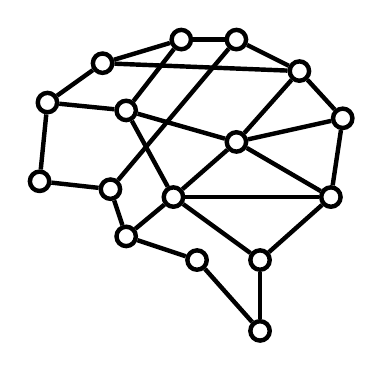
\begin{tikzpicture}
    \tikzstyle{hidden neuron}=[circle, draw, ultra thick, minimum size=7pt,inner sep=0pt];
    
    % \node[hidden neuron] (n1) at (0.5,0) {};
    \node[hidden neuron] (n2) at (1,0.3) {};
    
    \node[hidden neuron] (n3) at (0.2,1.2) {};
    \node[hidden neuron] (n4) at (1,1.2) {};
    
    \node[hidden neuron] (n5) at (1.9,2) {};
    \node[hidden neuron] (n6) at (-0.7,1.5) {};
    
    \node[hidden neuron] (n7) at (2.05,3) {};
    \node[hidden neuron] (n8) at (-0.9,2.1) {};
    
    \node[hidden neuron] (n9) at (1.5,3.6) {};
    \node[hidden neuron] (n10) at (-1.8,2.2) {};
    
    \node[hidden neuron] (n11) at (0.7,4) {};
    \node[hidden neuron] (n12) at (-1.7,3.2) {};
    
    \node[hidden neuron] (n13) at (0,4) {};
    \node[hidden neuron] (n14) at (-1,3.7) {};
    
    \node[hidden neuron] (n15) at (-0.7,3.1) {};
    \node[hidden neuron] (n16) at (0.7,2.7) {};
    \node[hidden neuron] (n17) at (-0.1,2) {};
    
    \draw[ultra thick] (n2) -- (n3);
    \draw[ultra thick] (n2) -- (n4);
    \draw[ultra thick] (n3) -- (n6);
    \draw[ultra thick] (n4) -- (n5);
    \draw[ultra thick] (n5) -- (n7);
    \draw[ultra thick] (n6) -- (n8);
    \draw[ultra thick] (n7) -- (n9);
    \draw[ultra thick] (n8) -- (n10);
    \draw[ultra thick] (n9) -- (n11);
    \draw[ultra thick] (n10) -- (n12);
    \draw[ultra thick] (n11) -- (n13);
    \draw[ultra thick] (n12) -- (n14);
    \draw[ultra thick] (n13) -- (n14);
    
    \draw[ultra thick] (n4) -- (n17);
    \draw[ultra thick] (n6) -- (n17);
    \draw[ultra thick] (n15) -- (n16);
    \draw[ultra thick] (n15) -- (n17);
    \draw[ultra thick] (n16) -- (n17);
    
    \draw[ultra thick] (n15) -- (n12);
    \draw[ultra thick] (n8) -- (n11);
    
    \draw[ultra thick] (n5) -- (n16);
    \draw[ultra thick] (n7) -- (n16);
    
    \draw[ultra thick] (n14) -- (n9);
    \draw[ultra thick] (n13) -- (n15);
    
    \draw[ultra thick] (n16) -- (n9);
    \draw[ultra thick] (n17) -- (n5);
    
\end{tikzpicture}}};
    \node[draw, fill=white, rounded corners] (nn_transfer_txt) at ($(encoder_transfer_c)+(0,0.325)$) {\tiny Encoder};
    
    \draw[->,thick, shorten >=5pt, shorten <=5pt] (spec_transfer.south) -- (encoder_transfer.north);
    
    \coordinate (nn_transfer_c) at ($(encoder_transfer_c) - (0, 2.5)$);
    \node[inner sep=0pt, color=green] (nn_transfer) at (nn_transfer_c) {\scalebox{.3}{\begin{tikzpicture}[shorten >=1pt]
    \tikzstyle{every pin edge}=[<-,shorten <=1pt]
    \tikzstyle{input neuron}=[circle, draw, thick, fill, minimum size=17pt,inner sep=0pt];
    \tikzstyle{output neuron}=[circle, draw, thick, double, minimum size=17pt,inner sep=0pt];
    \tikzstyle{hidden neuron}=[circle, draw, thick, minimum size=17pt,inner sep=0pt];


    
    % Draw the hidden layer nodes
    \foreach \name / \y in {1,...,3}
        \node[input neuron] (I-\name) at ($(0.5*\y + \y - 0.5, 0)$) {};
    
    \foreach \name / \y in {1,...,4}
        \node[hidden neuron] (H-\name) at ($(0.2*\y + \y - 0.5, -1.5cm)$) {};
    
    \foreach \name / \y in {1,...,2}
        \node[output neuron] (O-\name) at ($(1*\y + \y - 0.5, -3cm)$) {};
    
    \foreach \source in {1,...,3}
        \foreach \dest in {1,...,4}
            \draw[->,shorten >=1pt] (I-\source) -- (H-\dest);
    
    \foreach \source in {1,...,4}
        \foreach \dest in {1,...,2}
            \draw[->,shorten >=1pt] (H-\source) -- (O-\dest);
\end{tikzpicture}}};
    
    \draw[->,thick, shorten >=5pt, shorten <=5pt] (encoder_transfer.south) -- (nn_transfer.north);
    
    \coordinate (cce_c) at ($(nn_transfer_c) - (0, 2)$);
    \node[draw, rectangle, rounded corners, minimum width=2.5cm, minimum height=1cm, fill=green!50] (cce) at (cce_c) {Softmax-CCE};
    
    \draw[->,thick, shorten >=5pt, shorten <=5pt] (nn_transfer.south) -- (cce.north);
    
    \draw[->, thick, dashed, shorten >=5pt, shorten <=5pt] (encoder.east) .. controls ($(encoder.east) + (1.5,0.75)$) and ($(encoder.east) + (2,-1.5)$) .. (encoder_transfer.west);
    
    \node[] at ($(encoder.east) + (1,0.4)$) {\tiny \circled{6}};
    
\end{tikzpicture}